% arara: lualatex: { shell: yes, interaction: nonstopmode }
% arara: bibtex
% arara: lualatex: { shell: yes, interaction: nonstopmode }
% arara: lualatex: { shell: yes, interaction: nonstopmode }

%
%        ████████ ██   ██ ███████ ███████ ██ ███████ 
%           ██    ██   ██ ██      ██      ██ ██      
%           ██    ███████ █████   ███████ ██ ███████ 
%           ██    ██   ██ ██           ██ ██      ██ 
%           ██    ██   ██ ███████ ███████ ██ ███████ 
%

\documentclass{mscThesis}
% replace the previous line with the next to include a signature page
% use the option 'nosignatures' to turn off the signatures page
\usepackage{emielthesis}

%\mscFaculty{Mechanical, Maritime and Materials Engineering (3mE)}
\mscFaculty{Mechanical, Maritime and Materials Engineering}
\mscDepartment{Delft Center for Systems and Control (\textsmaller{DCSC})}%
\mscProgram{Systems and Control}

\mscName{E. B. Legrand}%
\mscDate{\today}%
\mscTitle{Thesis Title}%
\mscSubTitle{Optional Subtitle}%
\mscKeyWords{thesis, msc, subject}% only used in PDF properties
%\mscCoverPicture{media/template/COVER}% to place a picture ( here the example COVER.eps) on the cover page. Comment out if no picture is to be used

\mscThirdPartyText{The work in this thesis was supported by Rabobank. Their cooperation is hereby gratefully acknowledged.}
\mscThirdPartyLogo{media/template/RABO_LOGO.eps}

\mscSupervisorOne{prof.em.dr.ir.~M.~Mendel}
%\mscSupervisorTwo{Dr.ir.~M.Y.~Second Super}
%\mscSupervisorThree{}
\mscReaderOne{prof.dr.ir.~M.Y.~First Reader}
\mscReaderTwo{dr.ir.~F.S.T.~Reader-two}
\mscReaderThree{ir.~Th.~Reader-three}
%\mscReaderFour{}

% Finalize the thesis data
\setThesisInfo

% Use \includeonly{} to build only certain parts of your thesis
%\includeonly{introduction, real_chapter, empty_chapter, long_chapter}%

\lstset{lineskip=0pt plus 1pt minus 0pt} %%

% Externalize tikz
\tikzexternalize[prefix=media/cache/]

\begin{document}

%========================== Front matter ======================================

\frontmatter %
\maketitle

%
% Abstract (does not appear in the Table of Contents)
\chapter*{Abstract}%

This is an abstract.


\tocloflot
\chapter{Preface}
\thispagestyle{empty}
This thesis stands at the end of a long and twisty road with many dead ends. Indeed, even four months ago, I could not have envisioned what the final result turned out to be. This learned me an important lesson: that good results often come unexpected, but they never come for free. It takes some courage to invest so much time in studying subjects that are completely unfamiliar, and seem daunting at first. And even then, it takes innumerable mistakes to finally arrive at the correct result. 
However, this makes me all the more proud to present my work in this thesis; I sincerely hope that the reader shares in some of my enthusiasm, and finds it at least partially interesting.

Of course, I would never have succeeded in this task were it not for the support and assistance that I received along the way. First of all, I want to express my sincere gratitude to my supervisor prof. em. Mendel. The word `supervisor' definitely does not do justice to the substantial contributions that prof. em. Mendel made to this thesis, for most of the ideas presented are at least partially his, or the result of our frequent discussions. His deep intuition often directed us to the right answer, even if the intermediate steps were completely unknown to either of us. I can only be deeply grateful for all his time, inspiring ideas, and ever enduring enthusiasm over the past eighteen months. 

Second, I want to thank my parents for their intensive support, not only during my thesis but during my entire study, and for allowing me to pursue my dreams and ambitions. I have come to appreciate it deeply during the past year.

Third, I want to express how happy I am to have spent the past seven years in Delft with such excellent people. In particular, I want to thank my housemates Wout, Tim, Bram, Fréderic, Tine and Evert for making living in Delft so enjoyable --- may the Bronx flourish until eternity. Furthermore, my gratitude goes out to my fellow NunaX teammates and the the people of my student society, with whom I have built invaluable friendships over time.

Finally, I thank my peers in the economic engineering group for all their valuable feedback and suggestions, and for enduring the theoretical drivel they had to sit through during my presentations.

Mercikes!

\begin{flushright}
    Emiel Legrand
\end{flushright}
Delft, \mscdate




%
% Acknowledgements
\chapter{Acknowledgements}%

I would like to thank my supervisor \mscreaderone\ for his assistance during the writing of this thesis\ldots

By the way, it might make sense to combine the Preface and the Acknowledgements.  This is just a matter of taste, of course.

\vspace*{15mm}

Delft, University of Technology \hfill \mscname \\
\mscdate
%
% Dedication page. 
\cleardoublepage
\thispagestyle{empty}
\vspace*{\stretch{1}}

% Put your own motto here, or dedicate your work to your Mom or whatever...
%\begin{quote}
%\noindent Mathematics is the art of giving the same name to different things.
%\end{quote}
%\vspace{0.5 cm}
%\begin{quote}
%\noindent To doubt everything, or, to believe everything, are two equally convenient solutions; both dispense with the necessity of reflection.
%\end{quote}
%\vspace{1cm}
%--- \emph{Henri Poincaré}

%\begin{quote}
%Vainly, the author, you picture yourself as your artworks’ creator,
%over the Earth they have hovered forever remaining unnoticed.\\
%Space harbors many invisible shapes and inaudible motives,
%as it holds many delightful ensembles of colors and letters.
%\end{quote}
%--- \emph{Aleksey K. Tolstoy}
%\vspace{2cm}
%\begin{quote}
%    It is incredible how much a well-chosen word can economize
%    thought. Often one only needs to invent a new word, and this word becomes
%    a creator on its own right.
%\end{quote}
%--- \emph{Henri Poincaré, loosely cited by Vladimir I. Arnol'd}

\begin{quote}
    \hspace{-1em}\mbox{Man must sit in chair with open mouth for very long time before roast duck fly in.}
\end{quote}
--- \emph{Chinese proverb}
%\begin{quote}
%    If one were to bring ten of the wisest men in the world together and ask them what was the most stupid thing in existence, they would not be able to discover anything so stupid as astrology.
%\end{quote}
%--- \emph{David Hilbert}

\vspace{\stretch{3}}
\clearemptydoublepage


%========================== Main matter ======================================

\mainmatter

% Introduction
\chapter{Introduction}
\label{chap:intro}
Test \citet{texbook}
\index{emiel}

\subsection*{Notation check}
\begin{table}[h]
    \centering
    \begin{tabular}{lcccc}
    \toprule
        \textbf{Object} & \textbf{Roman lower} & \textbf{Roman upper} & \textbf{Greek lower} & \textbf{Greek upper} \\
    \midrule
        Standard & $a b c d e$ & $A B C D E$ & $\alpha \beta \gamma \delta \epsilon $ & $ \Gamma \Delta \Upsilon \Omega \Theta $\\
        Vector & $\vec{a} \vec{b} \vec{c} \vec{d} \vec{e}$ & $\vec{A} \vec{B} \vec{C} \vec{D} \vec{E}$ & $\vec{\alpha} \vec{\beta} \vec{\gamma} \vec{\delta} \vec{\epsilon} $ & $ \vec{\Gamma} \vec{\Delta} \vec{\Upsilon} \vec{\Omega} \vec{\Theta} $\\
        Tensor & $\tens{a} \tens{b} \tens{c} \tens{d} \tens{e}$ & $\tens{A} \tens{B} \tens{C} \tens{D} \tens{E}$ & $\tens{\alpha} \tens{\beta} \tens{\gamma} \tens{\delta} \tens{\epsilon} $ & $ \tens{\Gamma} \tens{\Delta} \tens{\Upsilon} \tens{\Omega} \tens{\Theta} $\\
    \bottomrule
    \end{tabular}
    \caption{Caption}
    \label{tab:my_label}
\end{table}

Christoffel symbol: $\christ$\\
Math constants: $\ii \ec \pic$\\
Variation: $\var S$

\part{Symplectic Economic Theory}
\chapter{Hamiltonian economics}

\section{Symplectic formulation}

\begin{aside}{Lie derivatives \& Max' question}
    The Lie derivative of the tautological form $\alpha = p\dd{q}$ with respect to the
    Hamiltonian vector field
    $$ X_H = \pdv{H}{p}\pdv{}{q} - \pdv{H}{p}\pdv{}{p}$$
    is denoted by
    $$ \lied{X_H}{\alpha}.$$
    Using Cartan's magic formula ($ \lied{V}{\theta} = \dd{(\intpr{V}{\theta})} + \intpr{V}{\dd{\theta}}$), this expression
    can be written as
    \begin{equation*} 
        \begin{split}
            \lied{X_H}{p\dd{q}} &= \dd{(\intpr{X_H}{p\dd{q}})} + \intpr{X_H}{\dd{(p\dd{q})}} \\
                                &= \dd{(\intpr{X_H}{p\dd{q}})} - \intpr{X_H}{\omega} \\
                                &= \dd{(\intpr{X_H}{p\dd{q}})} - \dd{H} \\
                                &= \dd{\qty(\pdv{H}{p}p)} - \dd{H} \\
                                &= \dd{(\dot{q}p)} - \dd{H} \\
                                &= \dd{(\dot{q}p - H)} \\
                                &= \dd{L} \\
        \end{split}
    \end{equation*}

    Explicitly in components:
    \begin{equation*}
        \lied{X_H}{\alpha} = \qty[X_H^{\nu}(\partial_{\nu}\alpha_{\mu}) + (\partial_{\mu} X_H^{\nu})\alpha_{\nu}]\dd{x}^{\mu}
    \end{equation*}
    \begin{equation*}
        \begin{split}
            \lied{X_H}{\alpha} =\, &\qty[\pdv{H}{p}\qty(\pdv{}{q}p) + \qty(\pdv{}{q}\pdv{H}{p})p - \pdv{H}{q}\qty(\pdv{}{p}p) - \qty(\pdv{}{q}\pdv{H}{q})0]\dd{q} \\
                                + &\qty[\pdv{H}{p}\qty(\pdv{}{q}0) + \qty(\pdv{}{p}\pdv{H}{p})p - \pdv{H}{q}\qty(\pdv{}{q} 0) - \qty(\pdv{}{p}\pdv{H}{q})0]\dd{p} \\
                               =\,&\qty[ \qty(\pdv{}{q}\pdv{H}{p})p - \pdv{H}{q}]\dd{q} + \qty[\qty(\pdv{}{p}\pdv{H}{p})p]\dd{p}\\
        \end{split}
    \end{equation*}
    Compare this with the expression using the Cartan equation:
    \begin{equation*}
        \begin{split}
            \dd{\qty(\pdv{H}{p}p - H)} &= \pdv{}{q}\qty(\pdv{H}{p}p)\dd{q} + \pdv{}{p}\qty(\pdv{H}{p}p)\dd{p} - \pdv{H}{q}\dd{q} - \pdv{H}{p}\dd{p}\\
                                       &= \qty[p\pdv{}{q}\qty(\pdv{H}{p}) + \pdv{H}{p}\pdv{p}{q} - \pdv{H}{q}]\dd{q} + \qty[p\pdv{}{p}\qty(\pdv{H}{p}) + \pdv{H}{p}\pdv{p}{p} - \pdv{H}{p}]\dd{p}
        \end{split}
    \end{equation*}
    which coincides with the previous expression.

\end{aside}

\section{The Liouville theorem}
This section explores the different forms in which the Liouville theorem appears, both in classical mechanics and the general study of differential equations.

\subsection{About divergence}
In this text, divergence appears in general levels of generalization, from the standard vector calculus definition to one in terms of differential forms that applies to curved spaces as well.

CHECK Foundations of mechanics p. 130 for a rigorous treatment of divergence on manifolds.

\section{Variational formulation}

\chapter{Lagrangian economics}

\part{Autonomous systems}
% \chapter{The Liouville theorem}

\section{The generalized Liouville theorem}
This section explores the different forms in which the Liouville theorem appears, both in classical mechanics and the general study of differential equations.

\subsection{About divergence}
In this text, divergence appears in general levels of generalization, from the standard vector calculus definition to one in terms of differential forms that applies to curved spaces as well.

\section{Harmonic oscillator}
Although the harmonic oscillator is a topic that has been studied in tremendous detail, also from a stochastic perspective because of its importance in quantum mechanics, it proves to be an instructive starting point for this research as well \cite{Dekker1975}. Several reasons apply, most importantly that the solutions may be obtained analytically and that the Hamiltonian phase space is two-dimensional, which allows for straightforward visualization of the result.

\subsection{The Hamiltonian vector field}
Although the Liouville theorem is usually expressed directly in terms of Poisson brackets (which, in turn, have a trivial form if expressed in Darboux coordinates), a slightly more insightful approach is taken here. More specifically, instead of applying the Poisson brackts directly, they are formulated like so:
$$ \poisson{f}{g} = X_g(f) = \lied{X_g}{f} $$
where $X_g$ is the Hamiltonian vector field associated to $g$. The definition of Poisson brackets in terms of Hamiltonian vector fields makes it easy to draw connection between fluid mechanics and the classical mechanics.

For the undamped harmonic oscillator, the configuration manifold $M$ is simply $\real$. As such, the cotangent bundle $T^*\!M = \real^2$. The Hamiltonian, being a smooth function on $T^*M$, is simply a 0-form given in Darboux coordinates $(p, q)$ by:
\begin{equation}
    \ham:\quad T^*M \to \real:\quad \ham(p, q) = \frac{m}{2}p^2 + \frac{k}{2}q^2.
\end{equation}
To apply Liouville's theorem, the Hamiltonian vector field $X_\ham$ associated with $\ham$ must be found. By definition, one can do this by virtue of the canonical isomorphism induced by the symplectic 2-form:
$$ \dd{\ham}(\cdot) = \omega(X_{\ham}, \cdot), $$
this isomorphism is sometimes denoted by $\raiseIndex{\omega}$, colloquially called the `musical isomorphism'. In terms of the interior product, this pairing takes the form \cite{Osborne2017,Abraham1978}
\begin{equation} 
    \intpr{X_H}{\omega} = \dd{H}.
    \label{eq:canonical_isomorphism}
\end{equation}
The differential 1-form $\dd{\ham}$ is
$$ \dd{\ham} = kq\dd{q} + \frac{p}{m}\dd{p}, $$ 
such that, by means of \cref{eq:canonical_isomorphism}, the Hamiltonian vector field becomes
$$ X_{\ham} =  \frac{p}{m}\pdv{}{q} - kq\pdv{}{p}. $$
Having found the Hamiltonian vector field, Liouville's theorem can be applied to to an arbitrary distribution $\rho$ over the phase space:
\begin{equation}
    \pdv{\rho}{t} = -\poisson{\rho}{H} = -X_H(\rho) = -\frac{p}{m}\pdv{\rho}{q} + kq\pdv{\rho}{p}.
    \label{eq:pde_ho}
\end{equation}
This is a simple transport equation without diffusion (that is, $\rho$ is a \emph{passive scalar}); hence, the initial probability distribution will simply `drift' along the streamlines of the Hamiltonian flow. As such, this problem is analogous to a flow that is purely characterized by convection. 

\subsection{Solution of the Liouville equation}
The convection equation may be readily solved using the method of characteristics.
\begin{aside}{The method of characteristics}
    \Cref{eq:pde_ho} is part of a larger class of linear first-order PDE's of the form\footnote{If the functions $a$ and $c$ depend on $\rho$, the equation is called \emph{semilinear}. This is, however, never the case for a PDE arising from the Liouville equation.} \cite[p. 207]{Farlow1989}. \begin{equation} \sum_{i=1}^n a_i(x_1, \ldots, x_n, \rho) \pdv{\rho}{x_i} = c(x_1, \ldots, x_n, \rho), \label{eq:fo_pde}\end{equation}
    which are traditionally solved using the \emph{method of characteristics}. This method attempts to find characteristic lines along which the solution is constant, as to convert the PDE problem into an ODE problem. More specifically, one whishes to find a parameterization of $x_i$ and $\rho$ such that:
    \begin{equation}
        \begin{split}
            \dv{x_i}{s} &= a_i\\
            \dv{\rho}{s} &= c.
        \end{split}
    \end{equation}
    Given this parameterization, the PDE can be easily rewritten as follows: \cite{Farlow1989}
    $$ \dv{\rho}{s} = \sum_{i = 1}^n \pdv{\rho}{x_i}\dv{x_i}{s}. $$
    The solution of the ODE problem then produces the trajectories for the characteristics. The reparameterization in terms of $s$ must be accompagnied by another reparameterization of the initial conditions in terms of the variable(s) $r_i$; essentially, $s$ provides the parameterization along the characteristic curves while $r_i$ is the parameterization of the initial curves. The expressions for $r_i$ are found by asserting that $x_i(0) = r_i$, and then solving for the integration constants that are still present in the found ODE solutions. Then, finally, one solves the ODE in terms of the characteristic parameterization $\qty(s, r_1, \ldots, r_n)$
    $$ \dv{\rho}{s} + c\qty(x_1(s, r), \ldots, x_n(s, r))\rho = 0, $$
    after which that solution can be written in terms of the old coordinates to obtain the solution of the PDE.
    \tcblower
    The former approach presents a `classical' engineering perspective of the method of characteristics. However, the underlying mechanism may also be explained using the language of exterior calculus and contact geometry, which already plays a prominent role in this text. As outlined by \citet{Burke1985}, the solution of a first-order PDE may be represented as an integral manifold of the \emph{differential ideal} of two particular differential forms\footnote{For an algebra $A$, an ideal is $R$ is a subset of a $A$ such that for all $a \in A$ and $x \in I$, it is true that $x \bullet a \in I$; i.e. it is closed under the multiplication operator $\bullet$ of the algebra $A$ \cite{Schuller2014}. In this case, the vector space is the space of 1-forms on the contact space $(\vec{x}, \pdv{\rho}{\vec{x}}, \rho)$. The $\bullet$ operation of the algebra of forms is the exterior multiplication (or wedge product); the term \emph{differential ideal} refers to the fact that the ideal is closed under the \emph{derivation} on the algebra as well. Here, the derivation on the algebra of forms is the exterior derivative.}.
    The PDE given by \cref{eq:fo_pde} is `encoded' in two particular 1-forms that will constitute the differential ideal. The purpose is to find a general expression for the associated vector field that generates the integral manifold. The first 1-form, $\theta$, contains the `total differential' of $\rho$:
    $$ \theta = \dd{\rho} - \sum_{i = 1}^n\underbrace{\pdv{\rho}{x_i}}_{\xi_i}\dd{x}_i. $$
    Secondly, the PDE itself (that is, the functions $a_i, c$) must be captured by another form, in this case the 0-form
    $$ \phi = \sum_{i = 1}^n a_i\xi_i - c, $$
    from which a 1-form can be constructed using the exterior derivative:
    $$ \dd{\phi} = \sum_{i=1}^n \qty( a_i\dd{\xi}_i + \pdv{\phi}{x_i}\dd{x}_i) + \pdv{\phi}{\rho}\dd{\rho}.$$
    The purpose is then to find characteristic vectors $v, w$, whose integral curves are the characteristics of the solution. The vectors $v, w$ must satisfy the conditions: \cite[p. 215]{Burke1985}
    \begin{equation}
        \intpr{v}{\dd{\phi}} = 0 \qquad \intpr{w}{\dd{\phi}} = 0
        \label{eq:v_cond_1}
    \end{equation}
    to ensure that it satisfies the PDE equation (this means that $v$ is tangent to the hypersurface given by $\phi$);
    \begin{equation}
        \intpr{v}{\theta} = 0 \qquad \intpr{w}{\theta} = 0,
        \label{eq:v_cond_2}
    \end{equation}
    to enforce that $\vec{\xi}$ are truly partial derivatives (they have no component pointing in the direction of the characteristics); and finally
    \begin{equation}
        \intpr{w}{\intpr{v}{\dd{\theta}}} = 0
        \label{eq:v_cond_3}
    \end{equation}
    to form a integral ideal. The integral manifold of the characteristic vectors then constitutes the solution of the PDE.
\end{aside}

As it turns out, the method of characteristics takes a particularly simple form for the harmonic oscillator (and Hamiltonian systems in general). The reparameterization in terms of $s$ is
\begin{equation}
        \dv{p}{s} = -kq \qquad \dv{q}{s} = \frac{p}{m} \qquad \dv{t}{s} = 1.
\end{equation}
which immediately yields $t = s + c_1$ (choose $c_1 = 0$ without loss of generalization), and the former two equations simply resort to a time-reversed solution of the Hamiltonian problem in terms of $p$ and $q$. Solving the ODE to obtain the characteristic lines is therefore, rather unsurprisingly, equivalent to finding the phase trajectories of the Hamiltonian system. For the harmonic oscillator, these trajectories are
\begin{equation}
    \begin{split}
        q(t) &= c_2\cos(\omega t) + \frac{c_3}{m\omega}\sin(\omega t)\\
        p(t) &= c_3\cos(\omega t) - m\omega c_1 \sin(\omega t). \\
    \end{split}
\end{equation}
Solving for $q(0) = r_1$ and $p(0) = r_2$, yields $r_1 = c_2$ and $r_2 = c_3$. Now, because the `forcing term' $c(\cdot)$ is not present in the Liouville equation (for autonomous systems), the solution of the second ODE is trivial:
$$ \rho(t) = \rho_0(r_1, \ldots, r_2), $$
\towrite{Jacobian?}\\
where $\rho_0$ is the initial distribution. It is an encouraging observation that the method of characteristics is easily extended towards non-autonomous systems, leaving the possibility for control action or external disturbances, which may well be of a stochastic nature themselves.

The solution to the Liouville equation is found by writing the initial distribution in terms of $p$, $q$ and $t$. Since $q$ and $p$ depend linearly on $r_1$ and $r_2$, this is a matter of taking the inverse of the associated matrix.
$$ 
    \mqty(q\\p) = 
    \underbrace{\mqty( 
        \cos(\omega t) & \frac{1}{m\omega}\sin(\omega t) \\
        -m\omega \sin(\omega t) & \cos(\omega t)
    )}_{\Phi(t)}
    \mqty(r_1\\r_2).
$$
This transformation matrix represents a symplectic transformation of the phase plane; symplectic matrices have a unit determinant\footnote{Due to the equivalence of $\spgroup{2}{\real}$ and $\slgroup{2, \real}$, having a unit determinant is a necessary and sufficient condition for a $2\times2$ matrix to be symplectic; this condition is only necessary for higher dimensional vector spaces \cite{Arnold1989}.}. More specifically, the above matrix is a `squeezed' rotation matrix Inversion and resubstitution of $t$ then yields:
$$ \mqty(r_1\\r_2) = \mqty(\cos(\omega t) & \frac{-1}{m\omega}\sin(\omega t) \\\  m\omega\sin(\omega t) & \cos(\omega t) )\mqty(q\\p),$$
this is the time-reversed flow of the Hamiltonian vector field; a counterclockwise rotation in the phase plane.

\paragraph{Motivation using exterior calculus}
In this section, the reasoning given by \citet{Burke1985} using exterior calculus is applied to the problem to motivate the validity of the solution given above. The solution is the integral manifold of tangent vectors to the contact space $(t,\,q,\,p,\,\xi_t,\,\xi_q,\,\xi_p,\,\rho)$, where $\xi_t = \pdv{\rho}{t}$ etc. As such, the tangent vectors $\vec{v}$ and $\vec{w}$ can be associated with seven-tuples:\footnote{With respect to the basis $\mqty(\pdv{}{t} & \pdv{}{q} & \pdv{}{p} & \pdv{}{\xi_t} & \pdv{}{\xi_q} & \pdv{}{\xi_p} & \pdv{}{\rho})$.}
$$\vec{v} = \mqty(v_t & v_q & v_p & v_{\xi_t} & v_{\xi_q} & v_{\xi_p} & v_{\rho})$$
$$\vec{w} = \mqty(w_t & w_q & w_p & w_{\xi_t} & w_{\xi_q} & w_{\xi_p} & w_{\rho}).$$
Likewise, the one-forms $\theta$ and $\dd{\phi}$ can be written as seven-tuples, too:\footnote{With respect to the basis $\mqty(\dd{t} & \dd{q} & \dd{p} & \dd{\xi_t} & \dd{\xi_q} & \dd{\xi_p} & \dd{\rho})$.}
$$\theta = \mqty(-\xi_t & -\xi_q & -\xi_p & 0 & 0 & 0 & 1)$$
$$\dd{\phi} = \mqty(\pdv{\phi}{t} & \pdv{\phi}{q} & \pdv{\phi}{p} & 1 & \frac{p}{m} & -kq & \pdv{\phi}{\rho}).$$

Applying the conditions \cref{eq:v_cond_1} and \cref{eq:v_cond_2} to $\vec{v}$ is simply equivalent to the application of a `dot product' (i.e. a duality pairing);
$$ \theta(\vec{v}) = 0 \iff v_\rho = v_t\xi_t + v_q\xi_q + v_p\xi_p. $$
$$ \dd{\phi}(\vec{v}) = 0 \iff \pdv{\phi}{t}v_t + \pdv{\phi}{q}v_q + \pdv{\phi}{p}v_p + v_{\xi_t} + \frac{p}{m} v_{\xi_q} - kq v_{\xi_p} + \pdv{\phi}{\rho}v_\rho = 0. $$
Finally, all the conditions on $\vec{w}$ can be combined into the following statement: since $\intpr{\vec{w}}{\theta} = 0$ and $\intpr{\vec{w}}{\dd{\phi}} = 0$, condition \cref{eq:v_cond_3} is equivalent to stating that the 1-form $\intpr{\vec{v}}{\dd{\theta}}$ is a linear combination of $\theta$ and $\dd{\phi}$ \cite{Burke1985}. Using the Lagrange multipliers $\lambda$ and $\mu$, the condition reverts to
$$\intpr{\vec{v}}{\dd{\theta}} = \lambda \theta + \mu \dd{\phi}.$$
Using the properties of the interior product and the exterior derivative, one obtains
$$ v_t\dd{\xi_t} - v_{\xi_t}\dd{t} + v_q\dd{\xi_q} - v_{\xi_q}\dd{q} + v_p\dd{\xi_p} - v_{\xi_p}\dd{p} = \lambda \theta + \mu \dd{\phi}. $$
A particular choice of the Lagrange multipliers can be made to cancel two of the seven components, in this case those in $\dd{\xi_t}$ and $\dd{\rho}$, respectively the fourth and last entry in the ordered tuple representation, $\lambda = -v_t\pdv{\phi}{\rho}$ and $\mu = v_t$ This results in five additional equations:
\begin{equation*}
    \begin{split}
        v_{\xi_t} &= -v_t\qty(\xi_t\pdv{\phi}{\rho} + \pdv{\phi}{t}) \\
        v_{\xi_q} &= -v_t\qty(\xi_q\pdv{\phi}{\rho} + \pdv{\phi}{q}) \\
        v_{\xi_p} &= -v_t\qty(\xi_p\pdv{\phi}{\rho} + \pdv{\phi}{p}) \\
        v_q &= \frac{p}{m}v_t\\
        v_p &= -kq v_t\\
    \end{split}
\end{equation*}
These equations, combined with the former two conditions can be used to determine $\vec{v}$ up to a factor (choose $v_t = 1$):
$$ \vec{v} = \mqty(1 & \frac{p}{m} & -kq 
                   & -\xi_t\pdv{\phi}{\rho} - \pdv{\phi}{t} & 
                   & -\xi_q\pdv{\phi}{\rho} - \pdv{\phi}{q} & 
                   & -\xi_p\pdv{\phi}{\rho} - \pdv{\phi}{p} & 0). $$
Now, observe that, because of the (semi-)linearity of the original equation, the vector $\vec{v}$ can be projected to the $(t, q, p)$-space (the other components have no influence on the solution). As such, one must find the integral curves of the projected vector field
$$ \pdv{}{t} + \frac{p}{m}\pdv{}{q} - kq\pdv{}{p}, $$
which is precisely the Hamiltonian vector field in the extended (contact) phase space, or to quote \citet[p. 237]{Arnold1989}, \emph{the velocity vector of the phase flow in extended phase space}; the integral lines are the \emph{vortex lines} of the integral invariant of Poincaré-Cartan $p\dd{q} - \ham\dd{t}$. Hence, to find a solution of the PDE problem, one strives to integrate the above vector field, where the initial conditions serve as parameters. The initial conditions can then be solved at the point $t=0$ for the initial solution. This is precisely the methodology that is applied \emph{ad hoc} in the previous section.

\subsection{Initial Gaussian distribution} 
The solution of the Liouville equation to any initial distribution is simply found by substituting the $(q,p)$ dependence with transformation stated above. This solution is simply obtained by effecting the substitution 
$$\mqty(q\\p) \mapsto \Phi^{-1}(t)\mqty(q\\p)$$
in the original distribution $\rho_0$. Alternatively, one can see this as an affine transformation of the original random variable in the other direction, that is, 
$$\mqty(q_0\\p_0) \mapsto \Phi(t)\mqty(q_0\\p_0) = \mqty(q\\p)$$
For example, an initial bivariate Gaussian distribution centered at some initial point $(q_0, p_0)$ with covariance matrix $\Sigma$ subject to the linear transformation $\Phi = \Phi(t)$ yields again a Gaussian: \cite{Schon2011}
\begin{equation}
    \mqty(q(t)\\p(t)) \quad \sim \quad \gaussian{\Phi\mqty(q_0\\p_0)}{\Phi\Sigma\Phi^\top}.
    \label{eq:ho_gaussian}
\end{equation}
This result is, after all, not quite a surprise: the Gaussian distribution is transported by the convective stream of the phase space fluid; the mean drifts along its original phase space trajectory as if it were a single particle. The variance changes continuously by the transform given by $\Phi$. Interestingly, because $\Phi$ has a unit determinant, $\det(\Phi\Sigma\Phi^\top) = \det(\Sigma)$; as such, the \emph{entropy} of the Gaussian remains constant throughout, and equal to its initial value
$$ \frac{1}{2}\log(\det(2\pic\ec\Sigma)). $$

\paragraph{Marginal distributions} \Cref{eq:ho_gaussian} represents a specific bivariate Gaussian distribution at any point in time. Therefore, the marginal time-dependent distributions of $p$ and $q$ as a function of time may readily be obtained from the joint distribution: \cite{Schon2011}
\begin{equation}
    \begin{split}
        q(t) &\sim \gaussian{\cos(\omega t)q_0 + \frac{1}{m\omega}\sin(\omega t)p_0}{\sigma_q\cos[2](\omega t) + \frac{\sigma_{pq}}{m\omega}\sin(2\omega t) + \frac{\sigma_p}{m^2\omega^2}\sin[2](\omega t)}, \\
        p(t) &\sim \gaussian{\cos(\omega t)p_0 - m\omega\sin(\omega t)q_0}{\sigma_p\cos[2](\omega t) - \sigma_{pq}m\omega\sin(2\omega t) + \sigma_q m^2\omega^2\sin[2](\omega t)}
    \end{split}
    \label{eq:ho_marginal}
\end{equation}
given that $\Sigma = \mqty(\sigma_q & \sigma_{qp}\\\sigma_{qp} & \sigma_p)$. \Cref{fig:pq_marginal_ho} shows the time-varying distribution of $q$ and $p$ in the form of the mean with a $2\sigma$-confidence interval.
\begin{figure}[h]
    \centering
    % This file was created by matlab2tikz.
%
%The latest updates can be retrieved from
%  http://www.mathworks.com/matlabcentral/fileexchange/22022-matlab2tikz-matlab2tikz
%where you can also make suggestions and rate matlab2tikz.
%
%
\begin{tikzpicture}

\begin{axis}[%
width=4.521in,
height=1.493in,
at={(0.758in,2.554in)},
scale only axis,
xmin=0,
xmax=10,
ymin=-4,
ymax=4,
ylabel={$p$},
axis background/.style={fill=white},
xmajorgrids,
ymajorgrids
]

\addplot[area legend, draw=none, fill=accent1!30, forget plot]
table[row sep=crcr] {%
x	y\\
0	1.4\\
0.101010101010101	1.6789684306215\\
0.202020202020202	1.94276597934578\\
0.303030303030303	2.18013606835973\\
0.404040404040404	2.38028536682771\\
0.505050505050505	2.5335866662196\\
0.606060606060606	2.63222493279872\\
0.707070707070707	2.67073689994706\\
0.808080808080808	2.64640236969229\\
0.909090909090909	2.55945655172435\\
1.01010101010101	2.41310639226938\\
1.11111111111111	2.21334884793295\\
1.21212121212121	1.96860424283847\\
1.31313131313131	1.68919199794734\\
1.41414141414141	1.38668800928683\\
1.51515151515152	1.07321182118515\\
1.61616161616162	0.760696787253349\\
1.71717171717172	0.460197239763601\\
1.81818181818182	0.181283241365004\\
1.91919191919192	-0.0684339397283654\\
2.02020202020202	-0.283613299491702\\
2.12121212121212	-0.461313486843013\\
2.22222222222222	-0.600935806726432\\
2.32323232323232	-0.703991477115071\\
2.42424242424242	-0.773717738612815\\
2.52525252525253	-0.814579263464277\\
2.62626262626263	-0.831700095677602\\
2.72727272727273	-0.830276373898543\\
2.82828282828283	-0.815020949143664\\
2.92929292929293	-0.789687654955511\\
3.03030303030303	-0.756715705599894\\
3.13131313131313	-0.717024095732327\\
3.23232323232323	-0.669972829630974\\
3.33333333333333	-0.613493395240989\\
3.43434343434343	-0.544376304446184\\
3.53535353535354	-0.458689947094383\\
3.63636363636364	-0.352293569917175\\
3.73737373737374	-0.221398835865542\\
3.83838383838384	-0.0631298366915798\\
3.93939393939394	0.123968993510884\\
4.04040404040404	0.339523837958311\\
4.14141414141414	0.581060420003861\\
4.24242424242424	0.843899005122564\\
4.34343434343434	1.12123021958978\\
4.44444444444444	1.40437172333894\\
4.54545454545455	1.68319094541709\\
4.64646464646465	1.94666533797632\\
4.74747474747475	2.1835400496689\\
4.84848484848485	2.38303450670946\\
4.94949494949495	2.53554481222878\\
5.05050505050505	2.63328851546485\\
5.15151515151515	2.67084220514922\\
5.25252525252525	2.64553024541805\\
5.35353535353535	2.55763417697481\\
5.45454545454545	2.410405960299\\
5.55555555555556	2.20988325251225\\
5.65656565656566	1.96452008590512\\
5.75757575757576	1.68466044151707\\
5.85858585858586	1.38189415750843\\
5.95959595959596	1.06834342696751\\
6.06060606060606	0.755933123383594\\
6.16161616161616	0.45569895337446\\
6.26262626262626	0.177183924861741\\
6.36363636363636	-0.0720338715314932\\
6.46464646464646	-0.286650025540654\\
6.56565656565657	-0.463760308613019\\
6.66666666666667	-0.602800841353387\\
6.76767676767677	-0.705312792995926\\
6.86868686868687	-0.774556413523852\\
6.96969696969697	-0.815011006525015\\
7.07070707070707	-0.831806182173983\\
7.17171717171717	-0.830134687519967\\
7.27272727272727	-0.814697906099558\\
7.37373737373737	-0.789231700578743\\
7.47474747474747	-0.756152933466893\\
7.57575757575758	-0.716356353696694\\
7.67676767676768	-0.669178461804243\\
7.77777777777778	-0.612530541600733\\
7.87878787878788	-0.543188459117723\\
7.97979797979798	-0.457213280595502\\
8.08080808080808	-0.350465365903233\\
8.18181818181818	-0.219166291950278\\
8.28282828282828	-0.0604584401479727\\
8.38383838383838	0.127088277613444\\
8.48484848484848	0.343069238361175\\
8.58585858585859	0.584976416212211\\
8.68686868686869	0.848096104208731\\
8.78787878787879	1.12558756718173\\
8.88888888888889	1.40874243172953\\
8.98989898989899	1.6874097978935\\
9.09090909090909	1.95055833041535\\
9.19191919191919	2.1869350743384\\
9.29292929292929	2.38577238186116\\
9.39393939393939	2.53748982285803\\
9.49494949494949	2.63433765885351\\
9.5959595959596	2.67093242744145\\
9.6969696969697	2.64464310524738\\
9.7979797979798	2.55579756718953\\
9.8989898989899	2.40769274358704\\
10	2.20640690326466\\
10	0.612047983457317\\
9.8989898989899	0.668780438462062\\
9.7979797979798	0.716021832319933\\
9.6969696969697	0.755870957153892\\
9.5959595959596	0.789003052321844\\
9.49494949494949	0.814535495046958\\
9.39393939393939	0.830062617063296\\
9.29292929292929	0.831857573076923\\
9.19191919191919	0.815224756111912\\
9.09090909090909	0.774973164983124\\
8.98989898989899	0.705970459440479\\
8.88888888888889	0.603730071563279\\
8.78787878787879	0.464980291810285\\
8.68686868686869	0.288165010151271\\
8.58585858585859	0.0738307193868811\\
8.48484848484848	-0.175136907793281\\
8.38383838383838	-0.453451769415392\\
8.28282828282828	-0.753552391504806\\
8.18181818181818	-1.06590933609954\\
8.08080808080808	-1.37949626384593\\
7.97979797979798	-1.68239260371256\\
7.87878787878788	-1.96247490403217\\
7.77777777777778	-2.20814641991139\\
7.67676767676768	-2.40905094833528\\
7.57575757575758	-2.55671765037164\\
7.47474747474747	-2.64508855190546\\
7.37373737373737	-2.67088920194069\\
7.27272727272727	-2.63381489302023\\
7.17171717171717	-2.53651896101665\\
7.07070707070707	-2.38440485441772\\
6.96969696969697	-2.18523868397601\\
6.86868686868687	-1.9486126325549\\
6.76767676767677	-1.68530083205725\\
6.66666666666667	-1.40655720688125\\
6.56565656565657	-1.12340871836548\\
6.46464646464646	-0.845997118830295\\
6.36363636363636	-0.583017777745445\\
6.26262626262626	-0.341295757303214\\
6.16161616161616	-0.125527780552347\\
6.06060606060606	0.0617950043749924\\
5.95959595959596	0.220283385733277\\
5.85858585858586	0.351380202819906\\
5.75757575757576	0.457952234325618\\
5.65656565656566	0.543782877169989\\
5.55555555555556	0.613012344959386\\
5.45454545454545	0.669575925105039\\
5.35353535353535	0.716690441281553\\
5.25252525252525	0.756434516299058\\
5.15151515151515	0.789459901717124\\
5.05050505050505	0.814859724617062\\
4.94949494949495	0.830205940464589\\
4.84848484848485	0.831753690489543\\
4.74747474747475	0.814795843125985\\
4.64646464646465	0.774137938828951\\
4.54545454545455	0.704653132836739\\
4.44444444444444	0.601869420127036\\
4.34343434343434	0.462538040376779\\
4.24242424242424	0.285132788391638\\
4.14141414141414	0.0702349443441764\\
4.04040404040404	-0.179232703720339\\
3.93939393939394	-0.457947444824706\\
3.83838383838384	-0.758314590238901\\
3.73737373737374	-1.07077759045577\\
3.63636363636364	-1.38429140786747\\
3.53535353535354	-1.68692690811495\\
3.43434343434343	-1.96656320055454\\
3.33333333333333	-2.21161739665469\\
3.23232323232323	-2.41175777607515\\
3.13131313131313	-2.55854714481653\\
3.03030303030303	-2.64596818495385\\
2.92929292929293	-2.6707914376276\\
2.82828282828283	-2.63275852808762\\
2.72727272727273	-2.53456737959379\\
2.62626262626263	-2.38166134281705\\
2.52525252525253	-2.18183917620081\\
2.42424242424242	-1.94471645184944\\
2.32323232323232	-1.68108014319735\\
2.22222222222222	-1.40218598606034\\
2.12121212121212	-1.11905207525923\\
2.02020202020202	-0.841801766705726\\
1.91919191919192	-0.579104345663495\\
1.81818181818182	-0.337753481980404\\
1.71717171717172	-0.12241191712817\\
1.61616161616162	0.0644629373843796\\
1.51515151515152	0.22251264339874\\
1.41414141414141	0.353205468795126\\
1.31313131313131	0.459426420798084\\
1.21212121212121	0.544968742873912\\
1.11111111111111	0.613973694150635\\
1.01010101010101	0.670369176644435\\
0.909090909090909	0.717357317701646\\
0.808080808080808	0.756996501313241\\
0.707070707070707	0.789914959506902\\
0.606060606060606	0.815181578218772\\
0.505050505050505	0.8303459858197\\
0.404040404040404	0.83164539539037\\
0.303030303030303	0.814361265089569\\
0.202020202020202	0.773295810592184\\
0.101010101010101	0.703327823987494\\
0	0.6\\
}--cycle;
\addplot [color=accent1, thick, forget plot]
  table[row sep=crcr]{%
0	1\\
0.101010101010101	1.1911481273045\\
0.202020202020202	1.35803089496898\\
0.303030303030303	1.49724866672465\\
0.404040404040404	1.60596538110904\\
0.505050505050505	1.68196632601965\\
0.606060606060606	1.72370325550875\\
0.707070707070707	1.73032592972698\\
0.808080808080808	1.70169943550277\\
0.909090909090909	1.638406934713\\
1.01010101010101	1.54173778445691\\
1.11111111111111	1.41366127104179\\
1.21212121212121	1.25678649285619\\
1.31313131313131	1.07430920937271\\
1.41414141414141	0.869946739040978\\
1.51515151515152	0.647862232291946\\
1.61616161616162	0.412579862318864\\
1.71717171717172	0.168892661317715\\
1.81818181818182	-0.0782351203076999\\
1.91919191919192	-0.32376914269593\\
2.02020202020202	-0.562707533098714\\
2.12121212121212	-0.790182781051123\\
2.22222222222222	-1.00156089639339\\
2.32323232323232	-1.19253581015621\\
2.42424242424242	-1.35921709523113\\
2.52525252525253	-1.49820921983254\\
2.62626262626263	-1.60668071924733\\
2.72727272727273	-1.68242187674617\\
2.82828282828283	-1.72388973861564\\
2.92929292929293	-1.73023954629155\\
3.03030303030303	-1.70134194527687\\
3.13131313131313	-1.63778562027443\\
3.23232323232323	-1.54086530285306\\
3.33333333333333	-1.41255539594784\\
3.43434343434343	-1.25546975250036\\
3.53535353535354	-1.07280842760466\\
3.63636363636364	-0.86829248889232\\
3.73737373737374	-0.646088213160654\\
3.83838383838384	-0.41072221346524\\
3.93939393939394	-0.166989225656911\\
4.04040404040404	0.0801455671189858\\
4.14141414141414	0.325647682174019\\
4.24242424242424	0.564515896757101\\
4.34343434343434	0.791884129983278\\
4.44444444444444	1.00312057173299\\
4.54545454545455	1.19392203912692\\
4.64646464646465	1.36040163840263\\
4.74747474747475	1.49916794639744\\
4.84848484848485	1.6073940985995\\
4.94949494949495	1.68287537634668\\
5.05050505050505	1.72407412004095\\
5.15151515151515	1.73015105343317\\
5.25252525252525	1.70098238085855\\
5.35353535353535	1.63716230912818\\
5.45454545454545	1.53999094270202\\
5.55555555555556	1.41144779873582\\
5.65656565656566	1.25415148153756\\
5.75757575757576	1.07130633792135\\
5.85858585858586	0.866637180164165\\
5.95959595959596	0.644313406350391\\
6.06060606060606	0.408864063879293\\
6.16161616161616	0.165085586411056\\
6.26262626262626	-0.0820559162207365\\
6.36363636363636	-0.327525824638469\\
6.46464646464646	-0.566323572185475\\
6.56565656565657	-0.79358451348925\\
6.66666666666667	-1.00467902411732\\
6.76767676767677	-1.19530681252659\\
6.86868686868687	-1.36158452303938\\
6.96969696969697	-1.50012484525051\\
7.07070707070707	-1.60810551829585\\
7.17171717171717	-1.68332682426831\\
7.27272727272727	-1.72425639955989\\
7.37373737373737	-1.73006045125972\\
7.47474747474747	-1.70062074268618\\
7.57575757575758	-1.63653700203417\\
7.67676767676768	-1.53911470506976\\
7.77777777777778	-1.41033848075606\\
7.87878787878788	-1.25283168157495\\
7.97979797979798	-1.06980294215403\\
8.08080808080808	-0.864980814874582\\
8.18181818181818	-0.642537814024909\\
8.28282828282828	-0.407005415826389\\
8.38383838383838	-0.163181745900974\\
8.48484848484848	0.083966165283947\\
8.58585858585859	0.329403567799546\\
8.68686868686869	0.568130557180001\\
8.78787878787879	0.79528392949601\\
8.88888888888889	1.0062362516464\\
8.98989898989899	1.19669012866699\\
9.09090909090909	1.36276574769924\\
9.19191919191919	1.50107991522515\\
9.29292929292929	1.60881497746904\\
9.39393939393939	1.68377621996066\\
9.49494949494949	1.72443657695023\\
9.5959595959596	1.72996773988165\\
9.6969696969697	1.70025703120063\\
9.7979797979798	1.63590969975473\\
9.8989898989899	1.53823659102455\\
10	1.40922744336099\\
};
\end{axis}

\begin{axis}[%
width=4.521in,
height=1.493in,
at={(0.758in,0.481in)},
scale only axis,
xmin=0,
xmax=10,
xlabel={$t$},
ymin=-2,
ymax=2,
ylabel={$q$},
axis background/.style={fill=white},
xmajorgrids,
ymajorgrids
]

\addplot[area legend, draw=none, fill=accent2!30, forget plot]
table[row sep=crcr] {%
x	y\\
0	1.4\\
0.101010101010101	1.24523723174286\\
0.202020202020202	1.06781404411508\\
0.303030303030303	0.874286122234442\\
0.404040404040404	0.671574786004928\\
0.505050505050505	0.466584493100268\\
0.606060606060606	0.265837219100639\\
0.707070707070707	0.075149401135605\\
0.808080808080808	-0.100626554664089\\
0.909090909090909	-0.257779585874282\\
1.01010101010101	-0.393826133541816\\
1.11111111111111	-0.507502537687224\\
1.21212121212121	-0.5986685416145\\
1.31313131313131	-0.668133780708945\\
1.41414141414141	-0.717425088687984\\
1.51515151515152	-0.748516889099221\\
1.61616161616162	-0.763549500098242\\
1.71717171717172	-0.764560667435395\\
1.81818181818182	-0.753254024705839\\
1.91919191919192	-0.730824603341383\\
2.02020202020202	-0.697856279374958\\
2.12121212121212	-0.654299586564517\\
2.22222222222222	-0.599531182273671\\
2.32323232323232	-0.532489015464303\\
2.42424242424242	-0.451870514550481\\
2.52525252525253	-0.35637544453743\\
2.62626262626263	-0.244970948751548\\
2.72727272727273	-0.117154036158765\\
2.82828282828283	0.0268134071881592\\
2.92929292929293	0.185720091909628\\
3.03030303030303	0.357290435492773\\
3.13131313131313	0.538152964044748\\
3.23232323232323	0.723898969171375\\
3.33333333333333	0.90923103777314\\
3.43434343434343	1.08819366867575\\
3.53535353535354	1.25447133067342\\
3.63636363636364	1.40173356201671\\
3.73737373737374	1.52400253399499\\
3.83838383838384	1.61601624711849\\
3.93939393939394	1.67356038906135\\
4.04040404040404	1.69374388033379\\
4.14141414141414	1.67519711580334\\
4.24242424242424	1.61817756672613\\
4.34343434343434	1.52457429273782\\
4.44444444444444	1.3978104808792\\
4.54545454545455	1.24265077847072\\
4.64646464646465	1.06492731090955\\
4.74747474747475	0.871204308776985\\
4.84848484848485	0.668405733276233\\
4.94949494949495	0.463432833456628\\
5.05050505050505	0.262798995917293\\
5.15151515151515	0.072307531008646\\
5.25252525252525	-0.103205675451584\\
5.35353535353535	-0.260048123313584\\
5.45454545454545	-0.39575540880158\\
5.55555555555556	-0.509082189811884\\
5.65656565656566	-0.599904392319313\\
5.75757575757576	-0.669044634982573\\
5.85858585858586	-0.718038786141252\\
5.95959595959596	-0.748865975562393\\
6.06060606060606	-0.763666912570992\\
6.16161616161616	-0.764475816366741\\
6.26262626262626	-0.752989616629297\\
6.36363636363636	-0.73039447761165\\
6.46464646464646	-0.697264440951598\\
6.56565656565657	-0.653540510103015\\
6.66666666666667	-0.598591350061981\\
6.76767676767677	-0.531349542318696\\
6.86868686868687	-0.450510615720768\\
6.96969696969697	-0.354776426019522\\
7.07070707070707	-0.243120349548452\\
7.17171717171717	-0.115049533164221\\
7.27272727272727	0.0291607072230669\\
7.37373737373737	0.188283303434015\\
7.47474747474747	0.360025744862141\\
7.57575757575758	0.540999840864647\\
7.67676767676768	0.726781789198574\\
7.77777777777778	0.912062052711267\\
7.87878787878788	1.09087714649842\\
7.97979797979798	1.25690859139037\\
8.08080808080808	1.40382855614821\\
8.18181818181818	1.52566756083502\\
8.28282828282828	1.61717739134229\\
8.38383838383838	1.67416226901658\\
8.48484848484848	1.69375334841189\\
8.58585858585859	1.67460562698182\\
8.68686868686869	1.61700202975626\\
8.78787878787879	1.52285633174365\\
8.88888888888889	1.39561415434773\\
8.98989898989899	1.24005891828025\\
9.09090909090909	1.06203674697859\\
9.19191919191919	0.8681203269563\\
9.29292929292929	0.665236168769889\\
9.39393939393939	0.460282225065467\\
9.49494949494949	0.259763216017957\\
9.5959595959596	0.0694692633657529\\
9.6969696969697	-0.105780309635565\\
9.7979797979798	-0.262311585404497\\
9.8989898989899	-0.397679313082961\\
10	-0.510656444831224\\
10	-0.91347698492755\\
9.8989898989899	-0.72822316052047\\
9.7979797979798	-0.542423717969696\\
9.6969696969697	-0.361394235588823\\
9.5959595959596	-0.189566049074442\\
9.49494949494949	-0.0303357020787671\\
9.39393939393939	0.113995827962832\\
9.29292929292929	0.242193573162006\\
9.19191919191919	0.353975486069541\\
9.09090909090909	0.449829329694701\\
8.98989898989899	0.530778587506762\\
8.88888888888889	0.598120334430853\\
8.78787878787879	0.653159969429379\\
8.68686868686869	0.696967576784992\\
8.58585858585859	0.73017847539449\\
8.48484848484848	0.752856421489113\\
8.38383838383838	0.764432292530998\\
8.28282828282828	0.763724367020703\\
8.18181818181818	0.749039082909655\\
8.08080808080808	0.71834400511956\\
7.97979797979798	0.669498252948896\\
7.87878787878788	0.600520368955644\\
7.77777777777778	0.509869991866594\\
7.67676767676768	0.396718032464092\\
7.57575757575758	0.261180489202122\\
7.47474747474747	0.104493554081426\\
7.37373737373737	-0.0708879458850132\\
7.27272727272727	-0.261280799316599\\
7.17171717171717	-0.461857396415879\\
7.07070707070707	-0.666821013426585\\
6.96969696969697	-0.869662587294024\\
6.86868686868687	-1.06348250620524\\
6.76767676767677	-1.24135552278803\\
6.66666666666667	-1.39671316729805\\
6.56565656565657	-1.52371630522678\\
6.46464646464646	-1.61759089430678\\
6.36363636363636	-1.67490252450467\\
6.26262626262626	-1.69374977554682\\
6.16161616161616	-1.67386244940334\\
6.06060606060606	-1.61659785306669\\
5.95959595959596	-1.52483595494528\\
5.85858585858586	-1.40278180879699\\
5.75757575757576	-1.25569053138684\\
5.65656565656566	-1.08953578795175\\
5.55555555555556	-0.910646736035452\\
5.45454545454545	-0.725340391204599\\
5.35353535353535	-0.539576255466956\\
5.25252525252525	-0.358657810892087\\
5.15151515151515	-0.187001317275307\\
5.05050505050505	-0.0279866086588157\\
4.94949494949495	0.116102269338722\\
4.84848484848485	0.244046141386194\\
4.74747474747475	0.355576412048442\\
4.64646464646465	0.451191010483231\\
4.54545454545455	0.531919684760894\\
4.44444444444444	0.599061632485146\\
4.34343434343434	0.653920382344321\\
4.24242424242424	0.697560675091595\\
4.14141414141414	0.730609853633186\\
4.04040404040404	0.753122151173115\\
3.93939393939394	0.764518608229144\\
3.83838383838384	0.763608623892153\\
3.73737373737374	0.748691911290106\\
3.63636363636364	0.717732480991852\\
3.53535353535354	0.668589811183701\\
3.43434343434343	0.599287116729927\\
3.33333333333333	0.50829303847999\\
3.23232323232323	0.39479144239346\\
3.13131313131313	0.258914488586847\\
3.03030303030303	0.10191667516975\\
2.92929292929293	-0.0737280167543281\\
2.82828282828283	-0.264317803339863\\
2.72727272727273	-0.46500853331114\\
2.62626262626263	-0.669990325181822\\
2.52525252525253	-0.872745488169163\\
2.42424242424242	-1.06637115793217\\
2.32323232323232	-1.24394468242316\\
2.22222222222222	-1.39890609260672\\
2.12121212121212	-1.52543029235641\\
2.02020202020202	-1.61876204576795\\
1.91919191919192	-1.67548940037382\\
1.81818181818182	-1.69373566303313\\
1.71717171717172	-1.67325608898951\\
1.61616161616162	-1.61543257516376\\
1.51515151515152	-1.52316730020602\\
1.41414141414141	-1.40068381844213\\
1.31313131313131	-1.25325099213432\\
1.21212121212121	-1.08685079163222\\
1.11111111111111	-0.907814960796065\\
1.01010101010101	-0.722457525729343\\
0.909090909090909	-0.536729968862932\\
0.808080808080808	-0.355923620474565\\
0.707070707070707	-0.184439628644314\\
0.606060606060606	-0.0256411036093851\\
0.505050505050505	0.118204833300217\\
0.404040404040404	0.2458947717236\\
0.303030303030303	0.357173523869525\\
0.202020202020202	0.452549128491877\\
0.101010101010101	0.533057535059867\\
0	0.6\\
}--cycle;
\addplot [color=accent2, thick, forget plot]
  table[row sep=crcr]{%
0	1\\
0.101010101010101	0.889147383401364\\
0.202020202020202	0.760181586303478\\
0.303030303030303	0.615729823051983\\
0.404040404040404	0.458734778864264\\
0.505050505050505	0.292394663200243\\
0.606060606060606	0.120098057745627\\
0.707070707070707	-0.0546451137543547\\
0.808080808080808	-0.228275087569327\\
0.909090909090909	-0.397254777368607\\
1.01010101010101	-0.558141829635579\\
1.11111111111111	-0.707658749241645\\
1.21212121212121	-0.842759666623361\\
1.31313131313131	-0.960692386421632\\
1.41414141414141	-1.05905445356506\\
1.51515151515152	-1.13584209465262\\
1.61616161616162	-1.189491037631\\
1.71717171717172	-1.21890837821245\\
1.81818181818182	-1.22349484386949\\
1.91919191919192	-1.2031570018576\\
2.02020202020202	-1.15830916257145\\
2.12121212121212	-1.08986493946046\\
2.22222222222222	-0.999218637440195\\
2.32323232323232	-0.888216848943734\\
2.42424242424242	-0.759120836241327\\
2.52525252525253	-0.614560466353296\\
2.62626262626263	-0.457480636966685\\
2.72727272727273	-0.291081284734952\\
2.82828282828283	-0.118752198075852\\
2.92929292929293	0.0559960375776501\\
3.03030303030303	0.229603555331261\\
3.13131313131313	0.398533726315797\\
3.23232323232323	0.559345205782417\\
3.33333333333333	0.708762038126565\\
3.43434343434343	0.843740392702839\\
3.53535353535354	0.96153057092856\\
3.63636363636364	1.05973302150428\\
3.73737373737374	1.13634722264255\\
3.83838383838384	1.18981243550532\\
3.93939393939394	1.21903949864525\\
4.04040404040404	1.22343301575345\\
4.14141414141414	1.20290348471826\\
4.24242424242424	1.15786912090886\\
4.34343434343434	1.08924733754107\\
4.44444444444444	0.998436056682171\\
4.54545454545455	0.887285231615806\\
4.64646464646465	0.758059160696389\\
4.74747474747475	0.613390360412714\\
4.84848484848485	0.456225937331214\\
4.94949494949495	0.289767551397675\\
5.05050505050505	0.117406193629238\\
5.15151515151515	-0.0573468931333307\\
5.25252525252525	-0.230931743171835\\
5.35353535353535	-0.39981218939027\\
5.45454545454545	-0.56054790000309\\
5.55555555555556	-0.709864462923668\\
5.65656565656566	-0.84472009013553\\
5.75757575757576	-0.962367583184709\\
5.85858585858586	-1.06041029746912\\
5.95959595959596	-1.13685096525384\\
6.06060606060606	-1.19013238281884\\
6.16161616161616	-1.21916913288504\\
6.26262626262626	-1.22336969608806\\
6.36363636363636	-1.20264850105816\\
6.46464646464646	-1.15742766762919\\
6.56565656565657	-1.0886284076649\\
6.66666666666667	-0.997652258680015\\
6.76767676767677	-0.886352532553364\\
6.86868686868687	-0.756996560963006\\
6.96969696969697	-0.612219506656773\\
7.07070707070707	-0.454970681487519\\
7.17171717171717	-0.28845346479005\\
7.27272727272727	-0.116060046046766\\
7.37373737373737	0.0586976787745007\\
7.47474747474747	0.232259649471784\\
7.57575757575758	0.401090165033384\\
7.67676767676768	0.561749910831333\\
7.77777777777778	0.710966022288931\\
7.87878787878788	0.845698757727031\\
7.97979797979798	0.963203422169631\\
8.08080808080808	1.06108628063388\\
8.18181818181818	1.13735332187234\\
8.28282828282828	1.19045087918149\\
8.38383838383838	1.21929728077379\\
8.48484848484848	1.2233048849505\\
8.58585858585859	1.20239205118816\\
8.68686868686869	1.15698480327063\\
8.78787878787879	1.08800815058652\\
8.88888888888889	0.99686724438929\\
8.98989898989899	0.885418752893506\\
9.09090909090909	0.755933038336645\\
9.19191919191919	0.61104790651292\\
9.29292929292929	0.453714870965948\\
9.39393939393939	0.287139026514149\\
9.49494949494949	0.114713756969595\\
9.5959595959596	-0.0600483928543445\\
9.6969696969697	-0.233587272612194\\
9.7979797979798	-0.402367651687097\\
9.8989898989899	-0.562951236801715\\
10	-0.712066714879387\\
};
\end{axis}

\begin{axis}[%
width=5.833in,
height=4.375in,
at={(0in,0in)},
scale only axis,
xmin=0,
xmax=1,
ymin=0,
ymax=1,
axis line style={draw=none},
ticks=none,
axis x line*=bottom,
axis y line*=left
]
\end{axis}
\end{tikzpicture}%

    \caption{The marginal distributions given by \cref{eq:ho_marginal}. The solid line represents the evolution of the mean, while the shaded area is a 95\% confidence interval, i.e. two standard deviations from the mean, given that the distribution is normal.}
    \label{fig:pq_marginal_ho}
\end{figure}
Clearly, the uncertainty for $p$ is largest when it's change is minimal; at the troughs and peaks of the sine wave; the same is true for $q$. Because both are a quarter cycle out of phase, their uncertainties 'exchange'. This is a compelling substantiation of Heisenberg's uncertainty principle, which states that canonical variables such as $p$ and $q$ cannot be measured simultaneously to arbitrary precision. [discuss with Max]
\begin{aside}{Fourier duality and the Heisenberg uncertainty principle}
    Bla bla bla
\end{aside}

\paragraph{Averages in time}
The motion of the harmonic oscillator is periodic. As such, the `average distribution over time' may be given a compact support over a single period. The distribution given by \cref{eq:ho_gaussian} may be considered to be a distribution \emph{conditioned} on time. To find the averaged distribution, the joint distribution $\Pr(p, q, t) = \Pr(p, q \mid t)\Pr(t)$ may be marginalized with respect to $t$:
$$ \rho(p, q) = \int \rho(p, q\mid t)\rho(t) \dd{t}. $$
Assuming that time is uniformly distributed over the period of the oscillations, the former expression is equivalent to:
\begin{equation}
    \begin{split}
        \rho(\vec{x}) &= \int_{0}^{\infty} \rho_\text{normal}\qty(\vec{x};\; \Phi(t)\vec{x}_0,\,\Phi(t)\Sigma\Phi(t)^\top)\rho_\text{uni}
        \qty(t;\; 0, T)\dd{t} \\
        &= \int_{0}^{\infty} \frac{1}{T\sqrt{4\pic^2\det(\Sigma)}}
        \ec^{-\frac{1}{2}\qty(\vec{x} - \Phi(t)\vec{x}_0)^\top(\Phi\Sigma\Phi^\top)^{-1}\qty(\vec{x} - \Phi(t)\vec{x}_0)}\, \qty(u_0(t) - u_T\qty(t)) \dd{t},\\
        &= \int_{0}^{T} \frac{1}{T\sqrt{4\pic^2\det(\Sigma)}}
        \ec^{-\frac{1}{2}\qty(\vec{x} - \Phi(t)\vec{x}_0)^\top(\Phi(t)\Sigma\Phi(t)^\top)^{-1}\qty(\vec{x} - \Phi(t)\vec{x}_0)} \dd{t},
    \end{split}
    \label{eq:time_averaged_pq}
\end{equation}
where $u_c$ refers to the Heaviside step delayed by $c$, and $\vec{x} = \qty(p\;\;q)$. Furthermore, probability density functions are unconventionally denoted by $\rho(\cdot\,;\,\cdot)$ to maintain the analogy with fluid dynamics, where the arguments and parameters are separated by a semicolon. In this case $\rho_\text{normal}(\vec{x}; \vec{\mu}, \Sigma)$ refers to a multivariate normal distribution with mean vector $\vec{\mu}$ and covariance matrix $\Sigma$, and $\rho_\text{uni}(t; a, b)$ refers to a scalar uniform distribution with bounds $a$ and $b$. \Cref{fig:time_average_ho} visualizes a numerical solution for this integral for some particular parameter values. 
\begin{figure}[h]
    \centering
    % This file was created by matlab2tikz.
%
%The latest updates can be retrieved from
%  http://www.mathworks.com/matlabcentral/fileexchange/22022-matlab2tikz-matlab2tikz
%where you can also make suggestions and rate matlab2tikz.
%
\begin{tikzpicture}

\begin{axis}[%
width=10cm,
height=10cm,
%at={(0.758in,0.481in)},
scale only axis,
xmin=-4,
xmax=4,
tick align=outside,
%xlabel style={font=\color{white!15!black}},
xlabel={$q$},
    zlabel={$\rho(q, p)$},
ymin=-4,
ymax=4,
%ylabel style={font=\color{white!15!black}},
ylabel={$p$},
zmin=0,
zmax=0.4,
view={-34.7625}{42.8186635952735},
axis background/.style={fill=white},
%axis x line*=bottom,
%axis y line*=left,
%axis z line*=left,
xmajorgrids,
ymajorgrids,
zmajorgrids,
xminorgrids,
yminorgrids,
zminorgrids,
]

\addplot3[%
surf,
shader=flat corner, ultra thin, draw=black, z buffer=sort, colormap name=accentmap, mesh/rows=100]
table[row sep=crcr, point meta=\thisrow{c}] {%
%
x	y	z	c\\
-4	-4	7.60516488830752e-15	7.60516488830752e-15\\
-3.91919191919192	-4	2.12568167645916e-14	2.12568167645916e-14\\
-3.83838383838384	-4	5.79405408928558e-14	5.79405408928558e-14\\
-3.75757575757576	-4	1.54029574595615e-13	1.54029574595615e-13\\
-3.67676767676768	-4	3.99390035708007e-13	3.99390035708007e-13\\
-3.5959595959596	-4	1.01016367656624e-12	1.01016367656624e-12\\
-3.51515151515152	-4	2.49242055695813e-12	2.49242055695813e-12\\
-3.43434343434343	-4	5.99973054097649e-12	5.99973054097649e-12\\
-3.35353535353535	-4	1.40923823819811e-11	1.40923823819811e-11\\
-3.27272727272727	-4	3.23036772619792e-11	3.23036772619792e-11\\
-3.19191919191919	-4	7.22782517015589e-11	7.22782517015589e-11\\
-3.11111111111111	-4	1.57875521620197e-10	1.57875521620197e-10\\
-3.03030303030303	-4	3.36684833229714e-10	3.36684833229714e-10\\
-2.94949494949495	-4	7.01041452207797e-10	7.01041452207797e-10\\
-2.86868686868687	-4	1.42558872083836e-09	1.42558872083836e-09\\
-2.78787878787879	-4	2.83162355256569e-09	2.83162355256569e-09\\
-2.70707070707071	-4	5.49465786245708e-09	5.49465786245708e-09\\
-2.62626262626263	-4	1.04180348618198e-08	1.04180348618198e-08\\
-2.54545454545455	-4	1.93041254702984e-08	1.93041254702984e-08\\
-2.46464646464646	-4	3.4963576505738e-08	3.4963576505738e-08\\
-2.38383838383838	-4	6.19110628809281e-08	6.19110628809281e-08\\
-2.3030303030303	-4	1.07200232104589e-07	1.07200232104589e-07\\
-2.22222222222222	-4	1.81547245655289e-07	1.81547245655289e-07\\
-2.14141414141414	-4	3.00776908206379e-07	3.00776908206379e-07\\
-2.06060606060606	-4	4.87593086017085e-07	4.87593086017085e-07\\
-1.97979797979798	-4	7.7362224692053e-07	7.7362224692053e-07\\
-1.8989898989899	-4	1.20160444396487e-06	1.20160444396487e-06\\
-1.81818181818182	-4	1.82751325922909e-06	1.82751325922909e-06\\
-1.73737373737374	-4	2.72228437188033e-06	2.72228437188033e-06\\
-1.65656565656566	-4	3.97273730774085e-06	3.97273730774085e-06\\
-1.57575757575758	-4	5.68120811871946e-06	5.68120811871946e-06\\
-1.4949494949495	-4	7.96339692278655e-06	7.96339692278655e-06\\
-1.41414141414141	-4	1.09439968080595e-05	1.09439968080595e-05\\
-1.33333333333333	-4	1.47498259409313e-05	1.47498259409313e-05\\
-1.25252525252525	-4	1.95004362347558e-05	1.95004362347558e-05\\
-1.17171717171717	-4	2.52965054241262e-05	2.52965054241262e-05\\
-1.09090909090909	-4	3.22067011478024e-05	3.22067011478024e-05\\
-1.01010101010101	-4	4.02540845117919e-05	4.02540845117919e-05\\
-0.929292929292929	-4	4.94034342970308e-05	4.94034342970308e-05\\
-0.848484848484849	-4	5.95510579887446e-05	5.95510579887446e-05\\
-0.767676767676768	-4	7.05186592452293e-05	7.05186592452293e-05\\
-0.686868686868687	-4	8.20526223977515e-05	8.20526223977515e-05\\
-0.606060606060606	-4	9.38296526245123e-05	9.38296526245123e-05\\
-0.525252525252525	-4	0.000105469109028853	0.000105469109028853\\
-0.444444444444444	-4	0.000116551651823861	0.000116551651823861\\
-0.363636363636364	-4	0.000126643082110921	0.000126643082110921\\
-0.282828282828283	-4	0.00013532158165959	0.00013532158165959\\
-0.202020202020202	-4	0.000142206054555384	0.000142206054555384\\
-0.121212121212121	-4	0.000146983007728295	0.000146983007728295\\
-0.0404040404040404	-4	0.000149429428098883	0.000149429428098883\\
0.0404040404040404	-4	0.000149429428098884	0.000149429428098884\\
0.121212121212121	-4	0.000146983007728295	0.000146983007728295\\
0.202020202020202	-4	0.000142206054555384	0.000142206054555384\\
0.282828282828283	-4	0.00013532158165959	0.00013532158165959\\
0.363636363636364	-4	0.000126643082110921	0.000126643082110921\\
0.444444444444444	-4	0.000116551651823861	0.000116551651823861\\
0.525252525252525	-4	0.000105469109028854	0.000105469109028854\\
0.606060606060606	-4	9.38296526245124e-05	9.38296526245124e-05\\
0.686868686868687	-4	8.20526223977514e-05	8.20526223977514e-05\\
0.767676767676768	-4	7.05186592452286e-05	7.05186592452286e-05\\
0.848484848484849	-4	5.95510579887429e-05	5.95510579887429e-05\\
0.929292929292929	-4	4.94034342970278e-05	4.94034342970278e-05\\
1.01010101010101	-4	4.02540845117798e-05	4.02540845117798e-05\\
1.09090909090909	-4	3.22067011477988e-05	3.22067011477988e-05\\
1.17171717171717	-4	2.52965054241255e-05	2.52965054241255e-05\\
1.25252525252525	-4	1.95004362347541e-05	1.95004362347541e-05\\
1.33333333333333	-4	1.47498259409314e-05	1.47498259409314e-05\\
1.41414141414141	-4	1.09439968080595e-05	1.09439968080595e-05\\
1.4949494949495	-4	7.96339692276187e-06	7.96339692276187e-06\\
1.57575757575758	-4	5.68120811872479e-06	5.68120811872479e-06\\
1.65656565656566	-4	3.97273730774157e-06	3.97273730774157e-06\\
1.73737373737374	-4	2.72228437188009e-06	2.72228437188009e-06\\
1.81818181818182	-4	1.82751325922888e-06	1.82751325922888e-06\\
1.8989898989899	-4	1.20160444396311e-06	1.20160444396311e-06\\
1.97979797979798	-4	7.73622246922877e-07	7.73622246922877e-07\\
2.06060606060606	-4	4.87593086602561e-07	4.87593086602561e-07\\
2.14141414141414	-4	3.00776908208119e-07	3.00776908208119e-07\\
2.22222222222222	-4	1.81547245656511e-07	1.81547245656511e-07\\
2.3030303030303	-4	1.07200232096757e-07	1.07200232096757e-07\\
2.38383838383838	-4	6.19110628694772e-08	6.19110628694772e-08\\
2.46464646464646	-4	3.49635765003031e-08	3.49635765003031e-08\\
2.54545454545455	-4	1.93041254730304e-08	1.93041254730304e-08\\
2.62626262626263	-4	1.04180355759082e-08	1.04180355759082e-08\\
2.70707070707071	-4	5.49465825088321e-09	5.49465825088321e-09\\
2.78787878787879	-4	2.8316235509238e-09	2.8316235509238e-09\\
2.86868686868687	-4	1.42558860209288e-09	1.42558860209288e-09\\
2.94949494949495	-4	7.01041388357676e-10	7.01041388357676e-10\\
3.03030303030303	-4	3.36677144751702e-10	3.36677144751702e-10\\
3.11111111111111	-4	1.57883499881669e-10	1.57883499881669e-10\\
3.19191919191919	-4	7.22850171994122e-11	7.22850171994122e-11\\
3.27272727272727	-4	3.23062228140597e-11	3.23062228140597e-11\\
3.35353535353535	-4	1.40925953956174e-11	1.40925953956174e-11\\
3.43434343434343	-4	5.99937487666212e-12	5.99937487666212e-12\\
3.51515151515152	-4	2.49216858083066e-12	2.49216858083066e-12\\
3.5959595959596	-4	1.01007619060359e-12	1.01007619060359e-12\\
3.67676767676768	-4	3.99380803658161e-13	3.99380803658161e-13\\
3.75757575757576	-4	1.54038333500094e-13	1.54038333500094e-13\\
3.83838383838384	-4	5.79470944087489e-14	5.79470944087489e-14\\
3.91919191919192	-4	2.12592957584516e-14	2.12592957584516e-14\\
4	-4	7.60563354008341e-15	7.60563354008341e-15\\
-4	-3.91919191919192	1.27222511669446e-14	1.27222511669446e-14\\
-3.91919191919192	-3.91919191919192	3.54833608447437e-14	3.54833608447437e-14\\
-3.83838383838384	-3.91919191919192	9.6505603374278e-14	9.6505603374278e-14\\
-3.75757575757576	-3.91919191919192	2.55973625144641e-13	2.55973625144641e-13\\
-3.67676767676768	-3.91919191919192	6.62209327735973e-13	6.62209327735973e-13\\
-3.5959595959596	-3.91919191919192	1.67104960445138e-12	1.67104960445138e-12\\
-3.51515151515152	-3.91919191919192	4.11350617704936e-12	4.11350617704936e-12\\
-3.43434343434343	-3.91919191919192	9.87879094322755e-12	9.87879094322755e-12\\
-3.35353535353535	-3.91919191919192	2.31481246555363e-11	2.31481246555363e-11\\
-3.27272727272727	-3.91919191919192	5.29312944336642e-11	5.29312944336642e-11\\
-3.19191919191919	-3.91919191919192	1.18131512521295e-10	1.18131512521295e-10\\
-3.11111111111111	-3.91919191919192	2.57362855435527e-10	2.57362855435527e-10\\
-3.03030303030303	-3.91919191919192	5.47411989132326e-10	5.47411989132326e-10\\
-2.94949494949495	-3.91919191919192	1.1369037476233e-09	1.1369037476233e-09\\
-2.86868686868687	-3.91919191919192	2.30567287434072e-09	2.30567287434072e-09\\
-2.78787878787879	-3.91919191919192	4.5673180210018e-09	4.5673180210018e-09\\
-2.70707070707071	-3.91919191919192	8.83839218169009e-09	8.83839218169009e-09\\
-2.62626262626263	-3.91919191919192	1.67113205786558e-08	1.67113205786558e-08\\
-2.54545454545455	-3.91919191919192	3.08783414533828e-08	3.08783414533828e-08\\
-2.46464646464646	-3.91919191919192	5.57681553686073e-08	5.57681553686073e-08\\
-2.38383838383838	-3.91919191919192	9.8467835308389e-08	9.8467835308389e-08\\
-2.3030303030303	-3.91919191919192	1.70007560934362e-07	1.70007560934362e-07\\
-2.22222222222222	-3.91919191919192	2.87078723376166e-07	2.87078723376166e-07\\
-2.14141414141414	-3.91919191919192	4.74230083303878e-07	4.74230083303878e-07\\
-2.06060606060606	-3.91919191919192	7.66535133851138e-07	7.66535133851138e-07\\
-1.97979797979798	-3.91919191919192	1.21264167972232e-06	1.21264167972232e-06\\
-1.8989898989899	-3.91919191919192	1.87800123351392e-06	1.87800123351392e-06\\
-1.81818181818182	-3.91919191919192	2.84793733294527e-06	2.84793733294527e-06\\
-1.73737373737374	-3.91919191919192	4.23006332962294e-06	4.23006332962294e-06\\
-1.65656565656566	-3.91919191919192	6.15542608893854e-06	6.15542608893854e-06\\
-1.57575757575758	-3.91919191919192	8.77766472449176e-06	8.77766472449176e-06\\
-1.4949494949495	-3.91919191919192	1.22694688762374e-05	1.22694688762374e-05\\
-1.41414141414141	-3.91919191919192	1.68157317313617e-05	1.68157317313617e-05\\
-1.33333333333333	-3.91919191919192	2.26030398219951e-05	2.26030398219951e-05\\
-1.25252525252525	-3.91919191919192	2.98055253469173e-05	2.98055253469173e-05\\
-1.17171717171717	-3.91919191919192	3.8567601939665e-05	3.8567601939665e-05\\
-1.09090909090909	-3.91919191919192	4.89846582486858e-05	4.89846582486858e-05\\
-1.01010101010101	-3.91919191919192	6.10833186505166e-05	6.10833186505166e-05\\
-0.929292929292929	-3.91919191919192	7.48033067845232e-05	7.48033067845232e-05\\
-0.848484848484849	-3.91919191919192	8.99831768288598e-05	8.99831768288598e-05\\
-0.767676767676768	-3.91919191919192	0.000106352139407933	0.000106352139407933\\
-0.686868686868687	-3.91919191919192	0.000123529867408129	0.000123529867408129\\
-0.606060606060606	-3.91919191919192	0.000141035529691276	0.000141035529691276\\
-0.525252525252525	-3.91919191919192	0.000158306422847804	0.000158306422847804\\
-0.444444444444444	-3.91919191919192	0.000174725549572731	0.000174725549572731\\
-0.363636363636364	-3.91919191919192	0.000189656452480241	0.000189656452480241\\
-0.282828282828283	-3.91919191919192	0.000202482690039529	0.000202482690039529\\
-0.202020202020202	-3.91919191919192	0.000212648662784066	0.000212648662784066\\
-0.121212121212121	-3.91919191919192	0.000219698160499688	0.000219698160499688\\
-0.0404040404040404	-3.91919191919192	0.000223307059657623	0.000223307059657623\\
0.0404040404040404	-3.91919191919192	0.000223307059657623	0.000223307059657623\\
0.121212121212121	-3.91919191919192	0.000219698160499689	0.000219698160499689\\
0.202020202020202	-3.91919191919192	0.000212648662784066	0.000212648662784066\\
0.282828282828283	-3.91919191919192	0.00020248269003953	0.00020248269003953\\
0.363636363636364	-3.91919191919192	0.000189656452480241	0.000189656452480241\\
0.444444444444444	-3.91919191919192	0.000174725549572732	0.000174725549572732\\
0.525252525252525	-3.91919191919192	0.000158306422847805	0.000158306422847805\\
0.606060606060606	-3.91919191919192	0.000141035529691276	0.000141035529691276\\
0.686868686868687	-3.91919191919192	0.000123529867408128	0.000123529867408128\\
0.767676767676768	-3.91919191919192	0.000106352139407931	0.000106352139407931\\
0.848484848484849	-3.91919191919192	8.99831768288569e-05	8.99831768288569e-05\\
0.929292929292929	-3.91919191919192	7.48033067845192e-05	7.48033067845192e-05\\
1.01010101010101	-3.91919191919192	6.10833186505069e-05	6.10833186505069e-05\\
1.09090909090909	-3.91919191919192	4.89846582486812e-05	4.89846582486812e-05\\
1.17171717171717	-3.91919191919192	3.85676019396625e-05	3.85676019396625e-05\\
1.25252525252525	-3.91919191919192	2.98055253469172e-05	2.98055253469172e-05\\
1.33333333333333	-3.91919191919192	2.26030398219951e-05	2.26030398219951e-05\\
1.41414141414141	-3.91919191919192	1.68157317313616e-05	1.68157317313616e-05\\
1.4949494949495	-3.91919191919192	1.22694688762372e-05	1.22694688762372e-05\\
1.57575757575758	-3.91919191919192	8.77766472448816e-06	8.77766472448816e-06\\
1.65656565656566	-3.91919191919192	6.1554260889393e-06	6.1554260889393e-06\\
1.73737373737374	-3.91919191919192	4.23006332962268e-06	4.23006332962268e-06\\
1.81818181818182	-3.91919191919192	2.84793733294519e-06	2.84793733294519e-06\\
1.8989898989899	-3.91919191919192	1.87800123351351e-06	1.87800123351351e-06\\
1.97979797979798	-3.91919191919192	1.21264167972304e-06	1.21264167972304e-06\\
2.06060606060606	-3.91919191919192	7.66535133852668e-07	7.66535133852668e-07\\
2.14141414141414	-3.91919191919192	4.74230083307336e-07	4.74230083307336e-07\\
2.22222222222222	-3.91919191919192	2.87078723378523e-07	2.87078723378523e-07\\
2.3030303030303	-3.91919191919192	1.70007560917046e-07	1.70007560917046e-07\\
2.38383838383838	-3.91919191919192	9.84678352970146e-08	9.84678352970146e-08\\
2.46464646464646	-3.91919191919192	5.57681553705725e-08	5.57681553705725e-08\\
2.54545454545455	-3.91919191919192	3.08783414635377e-08	3.08783414635377e-08\\
2.62626262626263	-3.91919191919192	1.67113205874234e-08	1.67113205874234e-08\\
2.70707070707071	-3.91919191919192	8.83839218393477e-09	8.83839218393477e-09\\
2.78787878787879	-3.91919191919192	4.56731801795858e-09	4.56731801795858e-09\\
2.86868686868687	-3.91919191919192	2.30567273008442e-09	2.30567273008442e-09\\
2.94949494949495	-3.91919191919192	1.13686438908514e-09	1.13686438908514e-09\\
3.03030303030303	-3.91919191919192	5.47423406419665e-10	5.47423406419665e-10\\
3.11111111111111	-3.91919191919192	2.57379410827954e-10	2.57379410827954e-10\\
3.19191919191919	-3.91919191919192	1.18139423776948e-10	1.18139423776948e-10\\
3.27272727272727	-3.91919191919192	5.29327145463066e-11	5.29327145463066e-11\\
3.35353535353535	-3.91919191919192	2.31474029381314e-11	2.31474029381314e-11\\
3.43434343434343	-3.91919191919192	9.87808080879057e-12	9.87808080879057e-12\\
3.51515151515152	-3.91919191919192	4.11321357908247e-12	4.11321357908247e-12\\
3.5959595959596	-3.91919191919192	1.67100155915315e-12	1.67100155915315e-12\\
3.67676767676768	-3.91919191919192	6.62231016918605e-13	6.62231016918605e-13\\
3.75757575757576	-3.91919191919192	2.5599437186382e-13	2.5599437186382e-13\\
3.83838383838384	-3.91919191919192	9.65143087995021e-14	9.65143087995021e-14\\
3.91919191919192	-3.91919191919192	3.54852179757351e-14	3.54852179757351e-14\\
4	-3.91919191919192	1.27220047229399e-14	1.27220047229399e-14\\
-4	-3.83838383838384	2.10380582625443e-14	2.10380582625443e-14\\
-3.91919191919192	-3.83838383838384	5.85525525646503e-14	5.85525525646503e-14\\
-3.83838383838384	-3.83838383838384	1.58900833630399e-13	1.58900833630399e-13\\
-3.75757575757576	-3.83838383838384	4.20528538473695e-13	4.20528538473695e-13\\
-3.67676767676768	-3.83838383838384	1.08542820285684e-12	1.08542820285684e-12\\
-3.5959595959596	-3.83838383838384	2.73266402227305e-12	2.73266402227305e-12\\
-3.51515151515152	-3.83838383838384	6.71104724528483e-12	6.71104724528483e-12\\
-3.43434343434343	-3.83838383838384	1.60787757762228e-11	1.60787757762228e-11\\
-3.35353535353535	-3.83838383838384	3.75854853144749e-11	3.75854853144749e-11\\
-3.27272727272727	-3.83838383838384	8.57330290197672e-11	8.57330290197672e-11\\
-3.19191919191919	-3.83838383838384	1.90854947497234e-10	1.90854947497234e-10\\
-3.11111111111111	-3.83838383838384	4.14743917129453e-10	4.14743917129453e-10\\
-3.03030303030303	-3.83838383838384	8.79822468568321e-10	8.79822468568321e-10\\
-2.94949494949495	-3.83838383838384	1.82233196440181e-09	1.82233196440181e-09\\
-2.86868686868687	-3.83838383838384	3.68591849651021e-09	3.68591849651021e-09\\
-2.78787878787879	-3.83838383838384	7.28150588645793e-09	7.28150588645793e-09\\
-2.70707070707071	-3.83838383838384	1.40516896187938e-08	1.40516896187938e-08\\
-2.62626262626263	-3.83838383838384	2.64938843765177e-08	2.64938843765177e-08\\
-2.54545454545455	-3.83838383838384	4.88150429603379e-08	4.88150429603379e-08\\
-2.46464646464646	-3.83838383838384	8.79097932610506e-08	8.79097932610506e-08\\
-2.38383838383838	-3.83838383838384	1.54769154114325e-07	1.54769154114325e-07\\
-2.3030303030303	-3.83838383838384	2.664321365087e-07	2.664321365087e-07\\
-2.22222222222222	-3.83838383838384	4.48578850964962e-07	4.48578850964962e-07\\
-2.14141414141414	-3.83838383838384	7.38821194802631e-07	7.38821194802631e-07\\
-2.06060606060606	-3.83838383838384	1.19066618852896e-06	1.19066618852896e-06\\
-1.97979797979798	-3.83838383838384	1.87800123351494e-06	1.87800123351494e-06\\
-1.8989898989899	-3.83838383838384	2.89978046789907e-06	2.89978046789907e-06\\
-1.81818181818182	-3.83838383838384	4.38438792630021e-06	4.38438792630021e-06\\
-1.73737373737374	-3.83838383838384	6.49294034732591e-06	6.49294034732591e-06\\
-1.65656565656566	-3.83838383838384	9.42060760100147e-06	9.42060760100147e-06\\
-1.57575757575758	-3.83838383838384	1.3394919593301e-05	1.3394919593301e-05\\
-1.4949494949495	-3.83838383838384	1.86700463678084e-05	1.86700463678084e-05\\
-1.41414141414141	-3.83838383838384	2.55162272462474e-05	2.55162272462474e-05\\
-1.33333333333333	-3.83838383838384	3.42039103238169e-05	3.42039103238169e-05\\
-1.25252525252525	-3.83838383838384	4.49827399241696e-05	4.49827399241696e-05\\
-1.17171717171717	-3.83838383838384	5.80562530885754e-05	5.80562530885754e-05\\
-1.09090909090909	-3.83838383838384	7.35539344825642e-05	7.35539344825642e-05\\
-1.01010101010101	-3.83838383838384	9.15030190999984e-05	9.15030190999984e-05\\
-0.929292929292929	-3.83838383838384	0.000111802995924611	0.000111802995924611\\
-0.848484848484849	-3.83838383838384	0.00013420603277696	0.00013420603277696\\
-0.767676767676768	-3.83838383838384	0.000158306422847805	0.000158306422847805\\
-0.686868686868687	-3.83838383838384	0.000183541608209862	0.000183541608209862\\
-0.606060606060606	-3.83838383838384	0.000209206388743757	0.000209206388743757\\
-0.525252525252525	-3.83838383838384	0.000234480664776197	0.000234480664776197\\
-0.444444444444444	-3.83838383838384	0.000258469630257566	0.000258469630257566\\
-0.363636363636364	-3.83838383838384	0.000280253906202108	0.000280253906202108\\
-0.282828282828283	-3.83838383838384	0.000298945864886132	0.000298945864886132\\
-0.202020202020202	-3.83838383838384	0.000313747508403952	0.000313747508403952\\
-0.121212121212121	-3.83838383838384	0.000324004852727801	0.000324004852727801\\
-0.0404040404040404	-3.83838383838384	0.00032925389390634	0.00032925389390634\\
0.0404040404040404	-3.83838383838384	0.00032925389390634	0.00032925389390634\\
0.121212121212121	-3.83838383838384	0.000324004852727801	0.000324004852727801\\
0.202020202020202	-3.83838383838384	0.000313747508403952	0.000313747508403952\\
0.282828282828283	-3.83838383838384	0.000298945864886133	0.000298945864886133\\
0.363636363636364	-3.83838383838384	0.000280253906202108	0.000280253906202108\\
0.444444444444444	-3.83838383838384	0.000258469630257566	0.000258469630257566\\
0.525252525252525	-3.83838383838384	0.000234480664776197	0.000234480664776197\\
0.606060606060606	-3.83838383838384	0.000209206388743757	0.000209206388743757\\
0.686868686868687	-3.83838383838384	0.000183541608209861	0.000183541608209861\\
0.767676767676768	-3.83838383838384	0.000158306422847802	0.000158306422847802\\
0.848484848484849	-3.83838383838384	0.000134206032776956	0.000134206032776956\\
0.929292929292929	-3.83838383838384	0.000111802995924608	0.000111802995924608\\
1.01010101010101	-3.83838383838384	9.15030190999878e-05	9.15030190999878e-05\\
1.09090909090909	-3.83838383838384	7.35539344836395e-05	7.35539344836395e-05\\
1.17171717171717	-3.83838383838384	5.8056253088574e-05	5.8056253088574e-05\\
1.25252525252525	-3.83838383838384	4.49827399241694e-05	4.49827399241694e-05\\
1.33333333333333	-3.83838383838384	3.42039103238168e-05	3.42039103238168e-05\\
1.41414141414141	-3.83838383838384	2.55162272462473e-05	2.55162272462473e-05\\
1.4949494949495	-3.83838383838384	1.86700463678184e-05	1.86700463678184e-05\\
1.57575757575758	-3.83838383838384	1.33949195933074e-05	1.33949195933074e-05\\
1.65656565656566	-3.83838383838384	9.42060760100239e-06	9.42060760100239e-06\\
1.73737373737374	-3.83838383838384	6.49294034732603e-06	6.49294034732603e-06\\
1.81818181818182	-3.83838383838384	4.38438792630037e-06	4.38438792630037e-06\\
1.8989898989899	-3.83838383838384	2.8997804679007e-06	2.8997804679007e-06\\
1.97979797979798	-3.83838383838384	1.87800123351755e-06	1.87800123351755e-06\\
2.06060606060606	-3.83838383838384	1.19066618853418e-06	1.19066618853418e-06\\
2.14141414141414	-3.83838383838384	7.38821194808736e-07	7.38821194808736e-07\\
2.22222222222222	-3.83838383838384	4.48578850942125e-07	4.48578850942125e-07\\
2.3030303030303	-3.83838383838384	2.6643213651194e-07	2.6643213651194e-07\\
2.38383838383838	-3.83838383838384	1.54769154116696e-07	1.54769154116696e-07\\
2.46464646464646	-3.83838383838384	8.79097932621102e-08	8.79097932621102e-08\\
2.54545454545455	-3.83838383838384	4.88150429749649e-08	4.88150429749649e-08\\
2.62626262626263	-3.83838383838384	2.64938843808043e-08	2.64938843808043e-08\\
2.70707070707071	-3.83838383838384	1.40516896125804e-08	1.40516896125804e-08\\
2.78787878787879	-3.83838383838384	7.28150587632897e-09	7.28150587632897e-09\\
2.86868686868687	-3.83838383838384	3.68591842273806e-09	3.68591842273806e-09\\
2.94949494949495	-3.83838383838384	1.82233206205269e-09	1.82233206205269e-09\\
3.03030303030303	-3.83838383838384	8.79822566593882e-10	8.79822566593882e-10\\
3.11111111111111	-3.83838383838384	4.14743914005265e-10	4.14743914005265e-10\\
3.19191919191919	-3.83838383838384	1.9086084337948e-10	1.9086084337948e-10\\
3.27272727272727	-3.83838383838384	8.57320237148951e-11	8.57320237148951e-11\\
3.35353535353535	-3.83838383838384	3.75836745528994e-11	3.75836745528994e-11\\
3.43434343434343	-3.83838383838384	1.60778769943425e-11	1.60778769943425e-11\\
3.51515151515152	-3.83838383838384	6.71084753326749e-12	6.71084753326749e-12\\
3.5959595959596	-3.83838383838384	2.73270754909219e-12	2.73270754909219e-12\\
3.67676767676768	-3.83838383838384	1.08548908171187e-12	1.08548908171187e-12\\
3.75757575757576	-3.83838383838384	4.20557235826106e-13	4.20557235826106e-13\\
3.83838383838384	-3.83838383838384	1.58907729538922e-13	1.58907729538922e-13\\
3.91919191919192	-3.83838383838384	5.85519683575891e-14	5.85519683575891e-14\\
4	-3.83838383838384	2.10365975475925e-14	2.10365975475925e-14\\
-4	-3.75757575757576	3.43916204415315e-14	3.43916204415315e-14\\
-3.91919191919192	-3.75757575757576	9.55160378610738e-14	9.55160378610738e-14\\
-3.83838383838384	-3.75757575757576	2.58652265796163e-13	2.58652265796163e-13\\
-3.75757575757576	-3.75757575757576	6.82997779797118e-13	6.82997779797118e-13\\
-3.67676767676768	-3.75757575757576	1.75887090537214e-12	1.75887090537214e-12\\
-3.5959595959596	-3.75757575757576	4.41781762484519e-12	4.41781762484519e-12\\
-3.51515151515152	-3.75757575757576	1.0823937468437e-11	1.0823937468437e-11\\
-3.43434343434343	-3.75757575757576	2.58707522343566e-11	2.58707522343566e-11\\
-3.35353535353535	-3.75757575757576	6.03286554645079e-11	6.03286554645079e-11\\
-3.27272727272727	-3.75757575757576	1.37271420542479e-10	1.37271420542479e-10\\
-3.19191919191919	-3.75757575757576	3.04816730200622e-10	3.04816730200622e-10\\
-3.11111111111111	-3.75757575757576	6.60664263265598e-10	6.60664263265598e-10\\
-3.03030303030303	-3.75757575757576	1.39783079195093e-09	1.39783079195093e-09\\
-2.94949494949495	-3.75757575757576	2.88752958037466e-09	2.88752958037466e-09\\
-2.86868686868687	-3.75757575757576	5.82458664246562e-09	5.82458664246562e-09\\
-2.78787878787879	-3.75757575757576	1.1474732808749e-08	1.1474732808749e-08\\
-2.70707070707071	-3.75757575757576	2.20817827197296e-08	2.20817827197296e-08\\
-2.62626262626263	-3.75757575757576	4.15162800254186e-08	4.15162800254186e-08\\
-2.54545454545455	-3.75757575757576	7.62741957259632e-08	7.62741957259632e-08\\
-2.46464646464646	-3.75757575757576	1.36961169815967e-07	1.36961169815967e-07\\
-2.38383838383838	-3.75757575757576	2.40418133112168e-07	2.40418133112168e-07\\
-2.3030303030303	-3.75757575757576	4.12648162018305e-07	4.12648162018305e-07\\
-2.22222222222222	-3.75757575757576	6.92679292557451e-07	6.92679292557451e-07\\
-2.14141414141414	-3.75757575757576	1.13742933151686e-06	1.13742933151686e-06\\
-2.06060606060606	-3.75757575757576	1.82751325922127e-06	1.82751325922127e-06\\
-1.97979797979798	-3.75757575757576	2.87374392823096e-06	2.87374392823096e-06\\
-1.8989898989899	-3.75757575757576	4.42382540326185e-06	4.42382540326185e-06\\
-1.81818181818182	-3.75757575757576	6.66844411316326e-06	6.66844411316326e-06\\
-1.73737373737374	-3.75757575757576	9.84566355223309e-06	9.84566355223309e-06\\
-1.65656565656566	-3.75757575757576	1.42422796990256e-05	1.42422796990256e-05\\
-1.57575757575758	-3.75757575757576	2.01906659376047e-05	2.01906659376047e-05\\
-1.4949494949495	-3.75757575757576	2.8059699680368e-05	2.8059699680368e-05\\
-1.41414141414141	-3.75757575757576	3.82386765337271e-05	3.82386765337271e-05\\
-1.33333333333333	-3.75757575757576	5.11137095956468e-05	5.11137095956468e-05\\
-1.25252525252525	-3.75757575757576	6.7036963392424e-05	6.7036963392424e-05\\
-1.17171717171717	-3.75757575757576	8.6290111680389e-05	8.6290111680389e-05\\
-1.09090909090909	-3.75757575757576	0.000109044510802502	0.000109044510802502\\
-1.01010101010101	-3.75757575757576	0.00013532158165949	0.00013532158165949\\
-0.929292929292929	-3.75757575757576	0.000164957615763471	0.000164957615763471\\
-0.848484848484849	-3.75757575757576	0.000197577504252011	0.000197577504252011\\
-0.767676767676768	-3.75757575757576	0.000232581622472103	0.000232581622472103\\
-0.686868686868687	-3.75757575757576	0.000269149251675918	0.000269149251675918\\
-0.606060606060606	-3.75757575757576	0.000306260535867779	0.000306260535867779\\
-0.525252525252525	-3.75757575757576	0.000342737193605781	0.000342737193605781\\
-0.444444444444444	-3.75757575757576	0.000377300235849434	0.000377300235849434\\
-0.363636363636364	-3.75757575757576	0.000408641022731827	0.000408641022731827\\
-0.282828282828283	-3.75757575757576	0.000435500366348921	0.000435500366348921\\
-0.202020202020202	-3.75757575757576	0.000456749261499735	0.000456749261499735\\
-0.121212121212121	-3.75757575757576	0.000471464348386571	0.000471464348386571\\
-0.0404040404040404	-3.75757575757576	0.000478991448282005	0.000478991448282005\\
0.0404040404040404	-3.75757575757576	0.000478991448282005	0.000478991448282005\\
0.121212121212121	-3.75757575757576	0.000471464348386572	0.000471464348386572\\
0.202020202020202	-3.75757575757576	0.000456749261499735	0.000456749261499735\\
0.282828282828283	-3.75757575757576	0.000435500366348922	0.000435500366348922\\
0.363636363636364	-3.75757575757576	0.000408641022731828	0.000408641022731828\\
0.444444444444444	-3.75757575757576	0.000377300235849435	0.000377300235849435\\
0.525252525252525	-3.75757575757576	0.000342737193605781	0.000342737193605781\\
0.606060606060606	-3.75757575757576	0.000306260535867778	0.000306260535867778\\
0.686868686868687	-3.75757575757576	0.000269149251675916	0.000269149251675916\\
0.767676767676768	-3.75757575757576	0.0002325816224721	0.0002325816224721\\
0.848484848484849	-3.75757575757576	0.000197577504252006	0.000197577504252006\\
0.929292929292929	-3.75757575757576	0.000164957615763473	0.000164957615763473\\
1.01010101010101	-3.75757575757576	0.00013532158165958	0.00013532158165958\\
1.09090909090909	-3.75757575757576	0.000109044510803574	0.000109044510803574\\
1.17171717171717	-3.75757575757576	8.62901116803869e-05	8.62901116803869e-05\\
1.25252525252525	-3.75757575757576	6.70369633924346e-05	6.70369633924346e-05\\
1.33333333333333	-3.75757575757576	5.11137095956466e-05	5.11137095956466e-05\\
1.41414141414141	-3.75757575757576	3.82386765337269e-05	3.82386765337269e-05\\
1.4949494949495	-3.75757575757576	2.80596996803682e-05	2.80596996803682e-05\\
1.57575757575758	-3.75757575757576	2.01906659376119e-05	2.01906659376119e-05\\
1.65656565656566	-3.75757575757576	1.42422796990274e-05	1.42422796990274e-05\\
1.73737373737374	-3.75757575757576	9.84566355223481e-06	9.84566355223481e-06\\
1.81818181818182	-3.75757575757576	6.66844411316212e-06	6.66844411316212e-06\\
1.8989898989899	-3.75757575757576	4.42382540326694e-06	4.42382540326694e-06\\
1.97979797979798	-3.75757575757576	2.87374392823759e-06	2.87374392823759e-06\\
2.06060606060606	-3.75757575757576	1.82751325923179e-06	1.82751325923179e-06\\
2.14141414141414	-3.75757575757576	1.13742933152506e-06	1.13742933152506e-06\\
2.22222222222222	-3.75757575757576	6.92679292562853e-07	6.92679292562853e-07\\
2.3030303030303	-3.75757575757576	4.12648162020567e-07	4.12648162020567e-07\\
2.38383838383838	-3.75757575757576	2.40418133110909e-07	2.40418133110909e-07\\
2.46464646464646	-3.75757575757576	1.36961169810609e-07	1.36961169810609e-07\\
2.54545454545455	-3.75757575757576	7.62741957316572e-08	7.62741957316572e-08\\
2.62626262626263	-3.75757575757576	4.15162800123087e-08	4.15162800123087e-08\\
2.70707070707071	-3.75757575757576	2.20817826976836e-08	2.20817826976836e-08\\
2.78787878787879	-3.75757575757576	1.14747327894938e-08	1.14747327894938e-08\\
2.86868686868687	-3.75757575757576	5.82458668627737e-09	5.82458668627737e-09\\
2.94949494949495	-3.75757575757576	2.88752968316901e-09	2.88752968316901e-09\\
3.03030303030303	-3.75757575757576	1.39783074149564e-09	1.39783074149564e-09\\
3.11111111111111	-3.75757575757576	6.60664059612465e-10	6.60664059612465e-10\\
3.19191919191919	-3.75757575757576	3.04816918048794e-10	3.04816918048794e-10\\
3.27272727272727	-3.75757575757576	1.37267327827925e-10	1.37267327827925e-10\\
3.35353535353535	-3.75757575757576	6.03261271033484e-11	6.03261271033484e-11\\
3.43434343434343	-3.75757575757576	2.58700353388797e-11	2.58700353388797e-11\\
3.51515151515152	-3.75757575757576	1.08239900584597e-11	1.08239900584597e-11\\
3.5959595959596	-3.75757575757576	4.41798176630423e-12	4.41798176630423e-12\\
3.67676767676768	-3.75757575757576	1.75895942110004e-12	1.75895942110004e-12\\
3.75757575757576	-3.75757575757576	6.83021745400161e-13	6.83021745400161e-13\\
3.83838383838384	-3.75757575757576	2.5865129821708e-13	2.5865129821708e-13\\
3.91919191919192	-3.75757575757576	9.55113375228997e-14	9.55113375228997e-14\\
4	-3.75757575757576	3.43888998717512e-14	3.43888998717512e-14\\
-4	-3.67676767676768	5.55811105286584e-14	5.55811105286584e-14\\
-3.91919191919192	-3.67676767676768	1.54040657740064e-13	1.54040657740064e-13\\
-3.83838383838384	-3.67676767676768	4.16235452138514e-13	4.16235452138514e-13\\
-3.75757575757576	-3.67676767676768	1.09668478480328e-12	1.09668478480328e-12\\
-3.67676767676768	-3.67676767676768	2.81780510753954e-12	2.81780510753954e-12\\
-3.5959595959596	-3.67676767676768	7.06114949108461e-12	7.06114949108461e-12\\
-3.51515151515152	-3.67676767676768	1.72593066014461e-11	1.72593066014461e-11\\
-3.43434343434343	-3.67676767676768	4.11529703588811e-11	4.11529703588811e-11\\
-3.35353535353535	-3.67676767676768	9.57315367494318e-11	9.57315367494318e-11\\
-3.27272727272727	-3.67676767676768	2.17287143978372e-10	2.17287143978372e-10\\
-3.19191919191919	-3.67676767676768	4.81268124404432e-10	4.81268124404432e-10\\
-3.11111111111111	-3.67676767676768	1.0404036559153e-09	1.0404036559153e-09\\
-3.03030303030303	-3.67676767676768	2.19547421889468e-09	2.19547421889468e-09\\
-2.94949494949495	-3.67676767676768	4.52306103103207e-09	4.52306103103207e-09\\
-2.86868686868687	-3.67676767676768	9.09878311115356e-09	9.09878311115356e-09\\
-2.78787878787879	-3.67676767676768	1.78753013807411e-08	1.78753013807411e-08\\
-2.70707070707071	-3.67676767676768	3.43019249717386e-08	3.43019249717386e-08\\
-2.62626262626263	-3.67676767676768	6.430697431345e-08	6.430697431345e-08\\
-2.54545454545455	-3.67676767676768	1.17802679287838e-07	1.17802679287838e-07\\
-2.46464646464646	-3.67676767676768	2.10909695342016e-07	2.10909695342016e-07\\
-2.38383838383838	-3.67676767676768	3.69124429479093e-07	3.69124429479093e-07\\
-2.3030303030303	-3.67676767676768	6.31652691318895e-07	6.31652691318895e-07\\
-2.22222222222222	-3.67676767676768	1.0570890726821e-06	1.0570890726821e-06\\
-2.14141414141414	-3.67676767676768	1.73051254441245e-06	1.73051254441245e-06\\
-2.06060606060606	-3.67676767676768	2.77187737235764e-06	2.77187737235764e-06\\
-1.97979797979798	-3.67676767676768	4.34529593396808e-06	4.34529593396808e-06\\
-1.8989898989899	-3.67676767676768	6.66844411315508e-06	6.66844411315508e-06\\
-1.81818181818182	-3.67676767676768	1.00209015544575e-05	1.00209015544575e-05\\
-1.73737373737374	-3.67676767676768	1.47498259409252e-05	1.47498259409252e-05\\
-1.65656565656566	-3.67676767676768	2.12710355020612e-05	2.12710355020612e-05\\
-1.57575757575758	-3.67676767676768	3.00634360022766e-05	3.00634360022766e-05\\
-1.4949494949495	-3.67676767676768	4.16548754965587e-05	4.16548754965587e-05\\
-1.41414141414141	-3.67676767676768	5.65980167130322e-05	5.65980167130322e-05\\
-1.33333333333333	-3.67676767676768	7.54357100187068e-05	7.54357100187068e-05\\
-1.25252525252525	-3.67676767676768	9.8656589286631e-05	9.8656589286631e-05\\
-1.17171717171717	-3.67676767676768	0.000126643082110921	0.000126643082110921\\
-1.09090909090909	-3.67676767676768	0.000159615538372358	0.000159615538372358\\
-1.01010101010101	-3.67676767676768	0.000197577504252012	0.000197577504252012\\
-0.929292929292929	-3.67676767676768	0.000240268060357027	0.000240268060357027\\
-0.848484848484849	-3.67676767676768	0.000287127396051742	0.000287127396051742\\
-0.767676767676768	-3.67676767676768	0.000337281278678807	0.000337281278678807\\
-0.686868686868687	-3.67676767676768	0.000389548775934777	0.000389548775934777\\
-0.606060606060606	-3.67676767676768	0.000442475602074525	0.000442475602074525\\
-0.525252525252525	-3.67676767676768	0.000494392993142126	0.000494392993142126\\
-0.444444444444444	-3.67676767676768	0.000543499361310183	0.000543499361310183\\
-0.363636363636364	-3.67676767676768	0.000587959457048156	0.000587959457048156\\
-0.282828282828283	-3.67676767676768	0.000626013690673765	0.000626013690673765\\
-0.202020202020202	-3.67676767676768	0.000656088886109446	0.000656088886109446\\
-0.121212121212121	-3.67676767676768	0.000676901225990838	0.000676901225990838\\
-0.0404040404040404	-3.67676767676768	0.000687542561581884	0.000687542561581884\\
0.0404040404040404	-3.67676767676768	0.000687542561581879	0.000687542561581879\\
0.121212121212121	-3.67676767676768	0.000676901225990839	0.000676901225990839\\
0.202020202020202	-3.67676767676768	0.000656088886109463	0.000656088886109463\\
0.282828282828283	-3.67676767676768	0.000626013690673767	0.000626013690673767\\
0.363636363636364	-3.67676767676768	0.000587959457048156	0.000587959457048156\\
0.444444444444444	-3.67676767676768	0.000543499361310184	0.000543499361310184\\
0.525252525252525	-3.67676767676768	0.000494392993142126	0.000494392993142126\\
0.606060606060606	-3.67676767676768	0.000442475602074524	0.000442475602074524\\
0.686868686868687	-3.67676767676768	0.000389548775934772	0.000389548775934772\\
0.767676767676768	-3.67676767676768	0.000337281278678803	0.000337281278678803\\
0.848484848484849	-3.67676767676768	0.000287127396051741	0.000287127396051741\\
0.929292929292929	-3.67676767676768	0.000240268060357027	0.000240268060357027\\
1.01010101010101	-3.67676767676768	0.000197577504252003	0.000197577504252003\\
1.09090909090909	-3.67676767676768	0.00015961553837235	0.00015961553837235\\
1.17171717171717	-3.67676767676768	0.000126643082110919	0.000126643082110919\\
1.25252525252525	-3.67676767676768	9.86565892865665e-05	9.86565892865665e-05\\
1.33333333333333	-3.67676767676768	7.54357100187066e-05	7.54357100187066e-05\\
1.41414141414141	-3.67676767676768	5.65980167130323e-05	5.65980167130323e-05\\
1.4949494949495	-3.67676767676768	4.16548754965475e-05	4.16548754965475e-05\\
1.57575757575758	-3.67676767676768	3.00634360022858e-05	3.00634360022858e-05\\
1.65656565656566	-3.67676767676768	2.12710355020659e-05	2.12710355020659e-05\\
1.73737373737374	-3.67676767676768	1.47498259409313e-05	1.47498259409313e-05\\
1.81818181818182	-3.67676767676768	1.00209015544665e-05	1.00209015544665e-05\\
1.8989898989899	-3.67676767676768	6.6684441131665e-06	6.6684441131665e-06\\
1.97979797979798	-3.67676767676768	4.34529593398059e-06	4.34529593398059e-06\\
2.06060606060606	-3.67676767676768	2.77187737237232e-06	2.77187737237232e-06\\
2.14141414141414	-3.67676767676768	1.73051254441958e-06	1.73051254441958e-06\\
2.22222222222222	-3.67676767676768	1.05708907268075e-06	1.05708907268075e-06\\
2.3030303030303	-3.67676767676768	6.31652691308934e-07	6.31652691308934e-07\\
2.38383838383838	-3.67676767676768	3.6912442946032e-07	3.6912442946032e-07\\
2.46464646464646	-3.67676767676768	2.10909695344201e-07	2.10909695344201e-07\\
2.54545454545455	-3.67676767676768	1.1780267925994e-07	1.1780267925994e-07\\
2.62626262626263	-3.67676767676768	6.43069742683706e-08	6.43069742683706e-08\\
2.70707070707071	-3.67676767676768	3.43019249306893e-08	3.43019249306893e-08\\
2.78787878787879	-3.67676767676768	1.78753013560344e-08	1.78753013560344e-08\\
2.86868686868687	-3.67676767676768	9.09878306266826e-09	9.09878306266826e-09\\
2.94949494949495	-3.67676767676768	4.52306105764785e-09	4.52306105764785e-09\\
3.03030303030303	-3.67676767676768	2.19547423977384e-09	2.19547423977384e-09\\
3.11111111111111	-3.67676767676768	1.04040317836325e-09	1.04040317836325e-09\\
3.19191919191919	-3.67676767676768	4.81267843301408e-10	4.81267843301408e-10\\
3.27272727272727	-3.67676767676768	2.17280669062056e-10	2.17280669062056e-10\\
3.35353535353535	-3.67676767676768	9.57292498609162e-11	9.57292498609162e-11\\
3.43434343434343	-3.67676767676768	4.1152895296324e-11	4.1152895296324e-11\\
3.51515151515152	-3.67676767676768	1.72597076424453e-11	1.72597076424453e-11\\
3.5959595959596	-3.67676767676768	7.06140389499734e-12	7.06140389499734e-12\\
3.67676767676768	-3.67676767676768	2.81788292920262e-12	2.81788292920262e-12\\
3.75757575757576	-3.67676767676768	1.09668491149607e-12	1.09668491149607e-12\\
3.83838383838384	-3.67676767676768	4.16221278724321e-13	4.16221278724321e-13\\
3.91919191919192	-3.67676767676768	1.54031811319752e-13	1.54031811319752e-13\\
4	-3.67676767676768	5.55780543778214e-14	5.55780543778214e-14\\
-4	-3.5959595959596	8.88081217358913e-14	8.88081217358913e-14\\
-3.91919191919192	-3.5959595959596	2.4560948422955e-13	2.4560948422955e-13\\
-3.83838383838384	-3.5959595959596	6.62238243471764e-13	6.62238243471764e-13\\
-3.75757575757576	-3.5959595959596	1.74100777543184e-12	1.74100777543184e-12\\
-3.67676767676768	-3.5959595959596	4.46323134982713e-12	4.46323134982713e-12\\
-3.5959595959596	-3.5959595959596	1.11585694797891e-11	1.11585694797891e-11\\
-3.51515151515152	-3.5959595959596	2.72099486399173e-11	2.72099486399173e-11\\
-3.43434343434343	-3.5959595959596	6.47226631529401e-11	6.47226631529401e-11\\
-3.35353535353535	-3.5959595959596	1.50190776437883e-10	1.50190776437883e-10\\
-3.27272727272727	-3.5959595959596	3.40046349114404e-10	3.40046349114404e-10\\
-3.19191919191919	-3.5959595959596	7.51252472771338e-10	7.51252472771338e-10\\
-3.11111111111111	-3.5959595959596	1.61983049745812e-09	1.61983049745812e-09\\
-3.03030303030303	-3.5959595959596	3.40912772242588e-09	3.40912772242588e-09\\
-2.94949494949495	-3.5959595959596	7.00443532171895e-09	7.00443532171895e-09\\
-2.86868686868687	-3.5959595959596	1.40516895982912e-08	1.40516895982912e-08\\
-2.78787878787879	-3.5959595959596	2.75284879864485e-08	2.75284879864485e-08\\
-2.70707070707071	-3.5959595959596	5.26757768468372e-08	5.26757768468372e-08\\
-2.62626262626263	-3.5959595959596	9.8467835349333e-08	9.8467835349333e-08\\
-2.54545454545455	-3.5959595959596	1.79852531163133e-07	1.79852531163133e-07\\
-2.46464646464646	-3.5959595959596	3.21044488315365e-07	3.21044488315365e-07\\
-2.38383838383838	-3.5959595959596	5.60185889008192e-07	5.60185889008192e-07\\
-2.3030303030303	-3.5959595959596	9.55681666121314e-07	9.55681666121314e-07\\
-2.22222222222222	-3.5959595959596	1.59444111295117e-06	1.59444111295117e-06\\
-2.14141414141414	-3.5959595959596	2.60208821479663e-06	2.60208821479663e-06\\
-2.06060606060606	-3.5959595959596	4.15491530024474e-06	4.15491530024474e-06\\
-1.97979797979798	-3.5959595959596	6.49294034732608e-06	6.49294034732608e-06\\
-1.8989898989899	-3.5959595959596	9.93290368447284e-06	9.93290368447284e-06\\
-1.81818181818182	-3.5959595959596	1.48794547059136e-05	1.48794547059136e-05\\
-1.73737373737374	-3.5959595959596	2.18322209067546e-05	2.18322209067546e-05\\
-1.65656565656566	-3.5959595959596	3.13860403758977e-05	3.13860403758977e-05\\
-1.57575757575758	-3.5959595959596	4.42215132632846e-05	4.42215132632846e-05\\
-1.4949494949495	-3.5959595959596	6.10833186504886e-05	6.10833186504886e-05\\
-1.41414141414141	-3.5959595959596	8.27445419638495e-05	8.27445419638495e-05\\
-1.33333333333333	-3.5959595959596	0.000109956583401046	0.000109956583401046\\
-1.25252525252525	-3.5959595959596	0.000143385991780333	0.000143385991780333\\
-1.17171717171717	-3.5959595959596	0.000183541608209862	0.000183541608209862\\
-1.09090909090909	-3.5959595959596	0.0002306974375959	0.0002306974375959\\
-1.01010101010101	-3.5959595959596	0.000284818368549322	0.000284818368549322\\
-0.929292929292929	-3.5959595959596	0.000345496911702215	0.000345496911702215\\
-0.848484848484849	-3.5959595959596	0.000411909265076228	0.000411909265076228\\
-0.767676767676768	-3.5959595959596	0.000482798104051037	0.000482798104051037\\
-0.686868686868687	-3.5959595959596	0.000556487547309969	0.000556487547309969\\
-0.606060606060606	-3.5959595959596	0.000630932943467041	0.000630932943467041\\
-0.525252525252525	-3.5959595959596	0.000703804766696084	0.000703804766696084\\
-0.444444444444444	-3.5959595959596	0.00077260240213208	0.00077260240213208\\
-0.363636363636364	-3.5959595959596	0.00083479036703929	0.00083479036703929\\
-0.282828282828283	-3.5959595959596	0.000887946938053545	0.000887946938053545\\
-0.202020202020202	-3.5959595959596	0.000929913535174338	0.000929913535174338\\
-0.121212121212121	-3.5959595959596	0.000958932724797319	0.000958932724797319\\
-0.0404040404040404	-3.5959595959596	0.000973763389486192	0.000973763389486192\\
0.0404040404040404	-3.5959595959596	0.000973763389486193	0.000973763389486193\\
0.121212121212121	-3.5959595959596	0.00095893272479732	0.00095893272479732\\
0.202020202020202	-3.5959595959596	0.000929913535174362	0.000929913535174362\\
0.282828282828283	-3.5959595959596	0.000887946938053547	0.000887946938053547\\
0.363636363636364	-3.5959595959596	0.000834790367039291	0.000834790367039291\\
0.444444444444444	-3.5959595959596	0.00077260240213201	0.00077260240213201\\
0.525252525252525	-3.5959595959596	0.000703804766696083	0.000703804766696083\\
0.606060606060606	-3.5959595959596	0.000630932943467039	0.000630932943467039\\
0.686868686868687	-3.5959595959596	0.000556487547309255	0.000556487547309255\\
0.767676767676768	-3.5959595959596	0.000482798104051033	0.000482798104051033\\
0.848484848484849	-3.5959595959596	0.000411909265076237	0.000411909265076237\\
0.929292929292929	-3.5959595959596	0.000345496911702203	0.000345496911702203\\
1.01010101010101	-3.5959595959596	0.000284818368549316	0.000284818368549316\\
1.09090909090909	-3.5959595959596	0.000230697437595891	0.000230697437595891\\
1.17171717171717	-3.5959595959596	0.000183541608209859	0.000183541608209859\\
1.25252525252525	-3.5959595959596	0.000143385991780332	0.000143385991780332\\
1.33333333333333	-3.5959595959596	0.000109956583401046	0.000109956583401046\\
1.41414141414141	-3.5959595959596	8.27445419638509e-05	8.27445419638509e-05\\
1.4949494949495	-3.5959595959596	6.10833186505167e-05	6.10833186505167e-05\\
1.57575757575758	-3.5959595959596	4.42215132632986e-05	4.42215132632986e-05\\
1.65656565656566	-3.5959595959596	3.13860403759091e-05	3.13860403759091e-05\\
1.73737373737374	-3.5959595959596	2.18322209067514e-05	2.18322209067514e-05\\
1.81818181818182	-3.5959595959596	1.48794547059134e-05	1.48794547059134e-05\\
1.8989898989899	-3.5959595959596	9.93290368447277e-06	9.93290368447277e-06\\
1.97979797979798	-3.5959595959596	6.49294034732607e-06	6.49294034732607e-06\\
2.06060606060606	-3.5959595959596	4.15491530017154e-06	4.15491530017154e-06\\
2.14141414141414	-3.5959595959596	2.60208821479663e-06	2.60208821479663e-06\\
2.22222222222222	-3.5959595959596	1.59444111294974e-06	1.59444111294974e-06\\
2.3030303030303	-3.5959595959596	9.55681666121153e-07	9.55681666121153e-07\\
2.38383838383838	-3.5959595959596	5.60185889008662e-07	5.60185889008662e-07\\
2.46464646464646	-3.5959595959596	3.21044488328442e-07	3.21044488328442e-07\\
2.54545454545455	-3.5959595959596	1.79852531097256e-07	1.79852531097256e-07\\
2.62626262626263	-3.5959595959596	9.84678352972522e-08	9.84678352972522e-08\\
2.70707070707071	-3.5959595959596	5.26757768019042e-08	5.26757768019042e-08\\
2.78787878787879	-3.5959595959596	2.75284879770555e-08	2.75284879770555e-08\\
2.86868686868687	-3.5959595959596	1.40516896327955e-08	1.40516896327955e-08\\
2.94949494949495	-3.5959595959596	7.00443538418691e-09	7.00443538418691e-09\\
3.03030303030303	-3.5959595959596	3.40912776314163e-09	3.40912776314163e-09\\
3.11111111111111	-3.5959595959596	1.61983052209852e-09	1.61983052209852e-09\\
3.19191919191919	-3.5959595959596	7.51252462873452e-10	7.51252462873452e-10\\
3.27272727272727	-3.5959595959596	3.40039791076689e-10	3.40039791076689e-10\\
3.35353535353535	-3.5959595959596	1.50189979547823e-10	1.50189979547823e-10\\
3.43434343434343	-3.5959595959596	6.47235295119444e-11	6.47235295119444e-11\\
3.51515151515152	-3.5959595959596	2.72106262165354e-11	2.72106262165354e-11\\
3.5959595959596	-3.5959595959596	1.11588050601682e-11	1.11588050601682e-11\\
3.67676767676768	-3.5959595959596	4.46324137220451e-12	4.46324137220451e-12\\
3.75757575757576	-3.5959595959596	1.74096788639167e-12	1.74096788639167e-12\\
3.83838383838384	-3.5959595959596	6.62211154573308e-13	6.62211154573308e-13\\
3.91919191919192	-3.5959595959596	2.45599738210761e-13	2.45599738210761e-13\\
4	-3.5959595959596	8.88068407977295e-14	8.88068407977295e-14\\
-4	-3.51515151515152	1.40298050850866e-13	1.40298050850866e-13\\
-3.91919191919192	-3.51515151515152	3.87194116047416e-13	3.87194116047416e-13\\
-3.83838383838384	-3.51515151515152	1.0417513228104e-12	1.0417513228104e-12\\
-3.75757575757576	-3.51515151515152	2.73272821656418e-12	2.73272821656418e-12\\
-3.67676767676768	-3.51515151515152	6.98985981806025e-12	6.98985981806025e-12\\
-3.5959595959596	-3.51515151515152	1.74351834382733e-11	1.74351834382733e-11\\
-3.51515151515152	-3.51515151515152	4.24150429623329e-11	4.24150429623329e-11\\
-3.43434343434343	-3.51515151515152	1.0064666592044e-10	1.0064666592044e-10\\
-3.35353535353535	-3.51515151515152	2.32978602476521e-10	2.32978602476521e-10\\
-3.27272727272727	-3.51515151515152	5.26164238815032e-10	5.26164238815032e-10\\
-3.19191919191919	-3.51515151515152	1.15949470335875e-09	1.15949470335875e-09\\
-3.11111111111111	-3.51515151515152	2.49350868648511e-09	2.49350868648511e-09\\
-3.03030303030303	-3.51515151515152	5.2339194345143e-09	5.2339194345143e-09\\
-2.94949494949495	-3.51515151515152	1.07244934420042e-08	1.07244934420042e-08\\
-2.86868686868687	-3.51515151515152	2.14550614962966e-08	2.14550614962966e-08\\
-2.78787878787879	-3.51515151515152	4.1914000488022e-08	4.1914000488022e-08\\
-2.70707070707071	-3.51515151515152	7.99726850902592e-08	7.99726850902592e-08\\
-2.62626262626263	-3.51515151515152	1.49058971051136e-07	1.49058971051136e-07\\
-2.54545454545455	-3.51515151515152	2.71452011084314e-07	2.71452011084314e-07\\
-2.46464646464646	-3.51515151515152	4.83097983190884e-07	4.83097983190884e-07\\
-2.38383838383838	-3.51515151515152	8.40383496442545e-07	8.40383496442545e-07\\
-2.3030303030303	-3.51515151515152	1.42927944317836e-06	1.42927944317836e-06\\
-2.22222222222222	-3.51515151515152	2.37714519292118e-06	2.37714519292118e-06\\
-2.14141414141414	-3.51515151515152	3.86722297128889e-06	3.86722297128889e-06\\
-2.06060606060606	-3.51515151515152	6.15542608894081e-06	6.15542608894081e-06\\
-1.97979797979798	-3.51515151515152	9.58842607844124e-06	9.58842607844124e-06\\
-1.8989898989899	-3.51515151515152	1.46213032287828e-05	1.46213032287828e-05\\
-1.81818181818182	-3.51515151515152	2.18322209067546e-05	2.18322209067546e-05\\
-1.73737373737374	-3.51515151515152	3.19308461008575e-05	3.19308461008575e-05\\
-1.65656565656566	-3.51515151515152	4.57567386691252e-05	4.57567386691252e-05\\
-1.57575757575758	-3.51515151515152	6.4263859884732e-05	6.4263859884732e-05\\
-1.4949494949495	-3.51515151515152	8.84878777271178e-05	8.84878777271178e-05\\
-1.41414141414141	-3.51515151515152	0.000119494177822567	0.000119494177822567\\
-1.33333333333333	-3.51515151515152	0.000158306422847802	0.000158306422847802\\
-1.25252525252525	-3.51515151515152	0.000205818000632995	0.000205818000632995\\
-1.17171717171717	-3.51515151515152	0.000262691483106778	0.000262691483106778\\
-1.09090909090909	-3.51515151515152	0.00032925389390634	0.00032925389390634\\
-1.01010101010101	-3.51515151515152	0.000405397708213942	0.000405397708213942\\
-0.929292929292929	-3.51515151515152	0.000490498666537364	0.000490498666537364\\
-0.848484848484849	-3.51515151515152	0.000583361366065085	0.000583361366065085\\
-0.767676767676768	-3.51515151515152	0.000682202066847614	0.000682202066847614\\
-0.686868686868687	-3.51515151515152	0.000784675295860972	0.000784675295860972\\
-0.606060606060606	-3.51515151515152	0.000887946938053545	0.000887946938053545\\
-0.525252525252525	-3.51515151515152	0.000988812020625473	0.000988812020625473\\
-0.444444444444444	-3.51515151515152	0.00108385086448924	0.00108385086448924\\
-0.363636363636364	-3.51515151515152	0.00116961323670535	0.00116961323670535\\
-0.282828282828283	-3.51515151515152	0.00124281705334368	0.00124281705334368\\
-0.202020202020202	-3.51515151515152	0.00130054638083883	0.00130054638083883\\
-0.121212121212121	-3.51515151515152	0.00134043312740373	0.00134043312740373\\
-0.0404040404040404	-3.51515151515152	0.00136080790186664	0.00136080790186664\\
0.0404040404040404	-3.51515151515152	0.00136080790186669	0.00136080790186669\\
0.121212121212121	-3.51515151515152	0.00134043312740373	0.00134043312740373\\
0.202020202020202	-3.51515151515152	0.00130054638083886	0.00130054638083886\\
0.282828282828283	-3.51515151515152	0.00124281705334368	0.00124281705334368\\
0.363636363636364	-3.51515151515152	0.00116961323670535	0.00116961323670535\\
0.444444444444444	-3.51515151515152	0.00108385086448917	0.00108385086448917\\
0.525252525252525	-3.51515151515152	0.000988812020625471	0.000988812020625471\\
0.606060606060606	-3.51515151515152	0.000887946938053542	0.000887946938053542\\
0.686868686868687	-3.51515151515152	0.00078467529586106	0.00078467529586106\\
0.767676767676768	-3.51515151515152	0.000682202066847616	0.000682202066847616\\
0.848484848484849	-3.51515151515152	0.000583361366065115	0.000583361366065115\\
0.929292929292929	-3.51515151515152	0.000490498666537419	0.000490498666537419\\
1.01010101010101	-3.51515151515152	0.000405397708213941	0.000405397708213941\\
1.09090909090909	-3.51515151515152	0.00032925389390633	0.00032925389390633\\
1.17171717171717	-3.51515151515152	0.000262691483106788	0.000262691483106788\\
1.25252525252525	-3.51515151515152	0.000205818000632996	0.000205818000632996\\
1.33333333333333	-3.51515151515152	0.000158306422847804	0.000158306422847804\\
1.41414141414141	-3.51515151515152	0.000119494177822573	0.000119494177822573\\
1.4949494949495	-3.51515151515152	8.84878777271534e-05	8.84878777271534e-05\\
1.57575757575758	-3.51515151515152	6.42638598847552e-05	6.42638598847552e-05\\
1.65656565656566	-3.51515151515152	4.5756738669126e-05	4.5756738669126e-05\\
1.73737373737374	-3.51515151515152	3.19308461008572e-05	3.19308461008572e-05\\
1.81818181818182	-3.51515151515152	2.18322209067543e-05	2.18322209067543e-05\\
1.8989898989899	-3.51515151515152	1.46213032287827e-05	1.46213032287827e-05\\
1.97979797979798	-3.51515151515152	9.58842607844615e-06	9.58842607844615e-06\\
2.06060606060606	-3.51515151515152	6.15542608893931e-06	6.15542608893931e-06\\
2.14141414141414	-3.51515151515152	3.86722297128889e-06	3.86722297128889e-06\\
2.22222222222222	-3.51515151515152	2.37714519291992e-06	2.37714519291992e-06\\
2.3030303030303	-3.51515151515152	1.42927944317866e-06	1.42927944317866e-06\\
2.38383838383838	-3.51515151515152	8.40383496474126e-07	8.40383496474126e-07\\
2.46464646464646	-3.51515151515152	4.83097983190972e-07	4.83097983190972e-07\\
2.54545454545455	-3.51515151515152	2.7145201108403e-07	2.7145201108403e-07\\
2.62626262626263	-3.51515151515152	1.49058971015502e-07	1.49058971015502e-07\\
2.70707070707071	-3.51515151515152	7.99726851020974e-08	7.99726851020974e-08\\
2.78787878787879	-3.51515151515152	4.19140005510469e-08	4.19140005510469e-08\\
2.86868686868687	-3.51515151515152	2.14550616438397e-08	2.14550616438397e-08\\
2.94949494949495	-3.51515151515152	1.07244935682084e-08	1.07244935682084e-08\\
3.03030303030303	-3.51515151515152	5.23391951409215e-09	5.23391951409215e-09\\
3.11111111111111	-3.51515151515152	2.49350873603635e-09	2.49350873603635e-09\\
3.19191919191919	-3.51515151515152	1.15947774636599e-09	1.15947774636599e-09\\
3.27272727272727	-3.51515151515152	5.26160775186888e-10	5.26160775186888e-10\\
3.35353535353535	-3.51515151515152	2.32980172763695e-10	2.32980172763695e-10\\
3.43434343434343	-3.51515151515152	1.0064832542298e-10	1.0064832542298e-10\\
3.51515151515152	-3.51515151515152	4.24157057787383e-11	4.24157057787383e-11\\
3.5959595959596	-3.51515151515152	1.74352389447271e-11	1.74352389447271e-11\\
3.67676767676768	-3.51515151515152	6.98975564406847e-12	6.98975564406847e-12\\
3.75757575757576	-3.51515151515152	2.73265036088507e-12	2.73265036088507e-12\\
3.83838383838384	-3.51515151515152	1.04172210410377e-12	1.04172210410377e-12\\
3.91919191919192	-3.51515151515152	3.87190428688511e-13	3.87190428688511e-13\\
4	-3.51515151515152	1.40301235729763e-13	1.40301235729763e-13\\
-4	-3.43434343434343	2.19151980522374e-13	2.19151980522374e-13\\
-3.91919191919192	-3.43434343434343	6.03544155478885e-13	6.03544155478885e-13\\
-3.83838383838384	-3.43434343434343	1.62036083075223e-12	1.62036083075223e-12\\
-3.75757575757576	-3.43434343434343	4.24122756213858e-12	4.24122756213858e-12\\
-3.67676767676768	-3.43434343434343	1.08240436255068e-11	1.08240436255068e-11\\
-3.5959595959596	-3.43434343434343	2.69370539943731e-11	2.69370539943731e-11\\
-3.51515151515152	-3.43434343434343	6.5376434575929e-11	6.5376434575929e-11\\
-3.43434343434343	-3.43434343434343	1.5475817821531e-10	1.5475817821531e-10\\
-3.35353535353535	-3.43434343434343	3.57354692102565e-10	3.57354692102565e-10\\
-3.27272727272727	-3.43434343434343	8.05029978703025e-10	8.05029978703025e-10\\
-3.19191919191919	-3.43434343434343	1.76948060921574e-09	1.76948060921574e-09\\
-3.11111111111111	-3.43434343434343	3.79536327046672e-09	3.79536327046672e-09\\
-3.03030303030303	-3.43434343434343	7.94525589157412e-09	7.94525589157412e-09\\
-2.94949494949495	-3.43434343434343	1.6235752078003e-08	1.6235752078003e-08\\
-2.86868686868687	-3.43434343434343	3.2390425434926e-08	3.2390425434926e-08\\
-2.78787878787879	-3.43434343434343	6.30977711318134e-08	6.30977711318134e-08\\
-2.70707070707071	-3.43434343434343	1.20044348422898e-07	1.20044348422898e-07\\
-2.62626262626263	-3.43434343434343	2.2309042653185e-07	2.2309042653185e-07\\
-2.54545454545455	-3.43434343434343	4.05057766679108e-07	4.05057766679108e-07\\
-2.46464646464646	-3.43434343434343	7.18686319550201e-07	7.18686319550201e-07\\
-2.38383838383838	-3.43434343434343	1.24635611139541e-06	1.24635611139541e-06\\
-2.3030303030303	-3.43434343434343	2.11311807700908e-06	2.11311807700908e-06\\
-2.22222222222222	-3.43434343434343	3.50338079922626e-06	3.50338079922626e-06\\
-2.14141414141414	-3.43434343434343	5.68120811872477e-06	5.68120811872477e-06\\
-2.06060606060606	-3.43434343434343	9.01356050825345e-06	9.01356050825345e-06\\
-1.97979797979798	-3.43434343434343	1.39949607665816e-05	1.39949607665816e-05\\
-1.8989898989899	-3.43434343434343	2.1271035502066e-05	2.1271035502066e-05\\
-1.81818181818182	-3.43434343434343	3.16572987659509e-05	3.16572987659509e-05\\
-1.73737373737374	-3.43434343434343	4.6148592364297e-05	4.6148592364297e-05\\
-1.65656565656566	-3.43434343434343	6.59140199814135e-05	6.59140199814135e-05\\
-1.57575757575758	-3.43434343434343	9.22722651343129e-05	9.22722651343129e-05\\
-1.4949494949495	-3.43434343434343	0.000126643082110874	0.000126643082110874\\
-1.41414141414141	-3.43434343434343	0.000170472608065736	0.000170472608065736\\
-1.33333333333333	-3.43434343434343	0.000225132919227134	0.000225132919227134\\
-1.25252525252525	-3.43434343434343	0.000291799711207673	0.000291799711207673\\
-1.17171717171717	-3.43434343434343	0.000371315706084739	0.000371315706084739\\
-1.09090909090909	-3.43434343434343	0.000464050827653031	0.000464050827653031\\
-1.01010101010101	-3.43434343434343	0.000569772747474762	0.000569772747474762\\
-0.929292929292929	-3.43434343434343	0.000687542561581885	0.000687542561581885\\
-0.848484848484849	-3.43434343434343	0.000815649760293415	0.000815649760293415\\
-0.767676767676768	-3.43434343434343	0.000951598206934671	0.000951598206934671\\
-0.686868686868687	-3.43434343434343	0.00109215073809931	0.00109215073809931\\
-0.606060606060606	-3.43434343434343	0.00123343469288564	0.00123343469288564\\
-0.525252525252525	-3.43434343434343	0.00137110481028344	0.00137110481028344\\
-0.444444444444444	-3.43434343434343	0.0015005542164832	0.0015005542164832\\
-0.363636363636364	-3.43434343434343	0.00161715932942871	0.00161715932942871\\
-0.282828282828283	-3.43434343434343	0.00171654096856286	0.00171654096856286\\
-0.202020202020202	-3.43434343434343	0.00179482210426508	0.00179482210426508\\
-0.121212121212121	-3.43434343434343	0.00184886262623605	0.00184886262623605\\
-0.0404040404040404	-3.43434343434343	0.0018764531686496	0.0018764531686496\\
0.0404040404040404	-3.43434343434343	0.00187645316864964	0.00187645316864964\\
0.121212121212121	-3.43434343434343	0.00184886262623605	0.00184886262623605\\
0.202020202020202	-3.43434343434343	0.00179482210426506	0.00179482210426506\\
0.282828282828283	-3.43434343434343	0.00171654096856286	0.00171654096856286\\
0.363636363636364	-3.43434343434343	0.00161715932942871	0.00161715932942871\\
0.444444444444444	-3.43434343434343	0.00150055421648313	0.00150055421648313\\
0.525252525252525	-3.43434343434343	0.00137110481028344	0.00137110481028344\\
0.606060606060606	-3.43434343434343	0.00123343469288563	0.00123343469288563\\
0.686868686868687	-3.43434343434343	0.00109215073809934	0.00109215073809934\\
0.767676767676768	-3.43434343434343	0.00095159820693469	0.00095159820693469\\
0.848484848484849	-3.43434343434343	0.000815649760293476	0.000815649760293476\\
0.929292929292929	-3.43434343434343	0.000687542561581871	0.000687542561581871\\
1.01010101010101	-3.43434343434343	0.000569772747474767	0.000569772747474767\\
1.09090909090909	-3.43434343434343	0.000464050827652889	0.000464050827652889\\
1.17171717171717	-3.43434343434343	0.000371315706084632	0.000371315706084632\\
1.25252525252525	-3.43434343434343	0.000291799711207675	0.000291799711207675\\
1.33333333333333	-3.43434343434343	0.000225132919227142	0.000225132919227142\\
1.41414141414141	-3.43434343434343	0.000170472608065739	0.000170472608065739\\
1.4949494949495	-3.43434343434343	0.000126643082110921	0.000126643082110921\\
1.57575757575758	-3.43434343434343	9.22722651343309e-05	9.22722651343309e-05\\
1.65656565656566	-3.43434343434343	6.59140199814142e-05	6.59140199814142e-05\\
1.73737373737374	-3.43434343434343	4.61485923642966e-05	4.61485923642966e-05\\
1.81818181818182	-3.43434343434343	3.16572987659507e-05	3.16572987659507e-05\\
1.8989898989899	-3.43434343434343	2.12710355020659e-05	2.12710355020659e-05\\
1.97979797979798	-3.43434343434343	1.39949607665813e-05	1.39949607665813e-05\\
2.06060606060606	-3.43434343434343	9.01356050825345e-06	9.01356050825345e-06\\
2.14141414141414	-3.43434343434343	5.68120811872478e-06	5.68120811872478e-06\\
2.22222222222222	-3.43434343434343	3.50338079922552e-06	3.50338079922552e-06\\
2.3030303030303	-3.43434343434343	2.11311807706955e-06	2.11311807706955e-06\\
2.38383838383838	-3.43434343434343	1.24635611139577e-06	1.24635611139577e-06\\
2.46464646464646	-3.43434343434343	7.18686319549942e-07	7.18686319549942e-07\\
2.54545454545455	-3.43434343434343	4.05057766691914e-07	4.05057766691914e-07\\
2.62626262626263	-3.43434343434343	2.2309042664639e-07	2.2309042664639e-07\\
2.70707070707071	-3.43434343434343	1.20044348627397e-07	1.20044348627397e-07\\
2.78787878787879	-3.43434343434343	6.30977711508337e-08	6.30977711508337e-08\\
2.86868686868687	-3.43434343434343	3.23904254433401e-08	3.23904254433401e-08\\
2.94949494949495	-3.43434343434343	1.62357521193651e-08	1.62357521193651e-08\\
3.03030303030303	-3.43434343434343	7.94525601297129e-09	7.94525601297129e-09\\
3.11111111111111	-3.43434343434343	3.79536515978288e-09	3.79536515978288e-09\\
3.19191919191919	-3.43434343434343	1.76946917911927e-09	1.76946917911927e-09\\
3.27272727272727	-3.43434343434343	8.05032018419704e-10	8.05032018419704e-10\\
3.35353535353535	-3.43434343434343	3.57358386687726e-10	3.57358386687726e-10\\
3.43434343434343	-3.43434343434343	1.54759904489596e-10	1.54759904489596e-10\\
3.51515151515152	-3.43434343434343	6.53766536701727e-11	6.53766536701727e-11\\
3.5959595959596	-3.43434343434343	2.69368037297768e-11	2.69368037297768e-11\\
3.67676767676768	-3.43434343434343	1.08238345555966e-11	1.08238345555966e-11\\
3.75757575757576	-3.43434343434343	4.24114562919902e-12	4.24114562919902e-12\\
3.83838383838384	-3.43434343434343	1.62035123074698e-12	1.62035123074698e-12\\
3.91919191919192	-3.43434343434343	6.0355483859635e-13	6.0355483859635e-13\\
4	-3.43434343434343	2.19161181435656e-13	2.19161181435656e-13\\
-4	-3.35353535353535	3.38496605502102e-13	3.38496605502102e-13\\
-3.91919191919192	-3.35353535353535	9.30267927877963e-13	9.30267927877963e-13\\
-3.83838383838384	-3.35353535353535	2.49218642038943e-12	2.49218642038943e-12\\
-3.75757575757576	-3.35353535353535	6.50893171992033e-12	6.50893171992033e-12\\
-3.67676767676768	-3.35353535353535	1.65743213511402e-11	1.65743213511402e-11\\
-3.5959595959596	-3.35353535353535	4.11530177518819e-11	4.11530177518819e-11\\
-3.51515151515152	-3.35353535353535	9.96446375547478e-11	9.96446375547478e-11\\
-3.43434343434343	-3.35353535353535	2.35310970461919e-10	2.35310970461919e-10\\
-3.35353535353535	-3.35353535353535	5.42024256963091e-10	5.42024256963091e-10\\
-3.27272727272727	-3.35353535353535	1.21797987782686e-09	1.21797987782686e-09\\
-3.19191919191919	-3.35353535353535	2.67026563216959e-09	2.67026563216959e-09\\
-3.11111111111111	-3.35353535353535	5.71252076081244e-09	5.71252076081244e-09\\
-3.03030303030303	-3.35353535353535	1.19265470696146e-08	1.19265470696146e-08\\
-2.94949494949495	-3.35353535353535	2.43046654981242e-08	2.43046654981242e-08\\
-2.86868686868687	-3.35353535353535	4.83525781010149e-08	4.83525781010149e-08\\
-2.78787878787879	-3.35353535353535	9.3924360755091e-08	9.3924360755091e-08\\
-2.70707070707071	-3.35353535353535	1.78173447563502e-07	1.78173447563502e-07\\
-2.62626262626263	-3.35353535353535	3.30137949259631e-07	3.30137949259631e-07\\
-2.54545454545455	-3.35353535353535	5.97615063862172e-07	5.97615063862172e-07\\
-2.46464646464646	-3.35353535353535	1.05708907246996e-06	1.05708907246996e-06\\
-2.38383838383838	-3.35353535353535	1.827513259229e-06	1.827513259229e-06\\
-2.3030303030303	-3.35353535353535	3.0886456711018e-06	3.0886456711018e-06\\
-2.22222222222222	-3.35353535353535	5.10433074459047e-06	5.10433074459047e-06\\
-2.14141414141414	-3.35353535353535	8.25053733696711e-06	8.25053733696711e-06\\
-2.06060606060606	-3.35353535353535	1.30470689126529e-05	1.30470689126529e-05\\
-1.97979797979798	-3.35353535353535	2.0190665937612e-05	2.0190665937612e-05\\
-1.8989898989899	-3.35353535353535	3.05858134072705e-05	3.05858134072705e-05\\
-1.81818181818182	-3.35353535353535	4.53681298782332e-05	4.53681298782332e-05\\
-1.73737373737374	-3.35353535353535	6.59140199814146e-05	6.59140199814146e-05\\
-1.65656565656566	-3.35353535353535	9.38296526245117e-05	9.38296526245117e-05\\
-1.57575757575758	-3.35353535353535	0.000130912619003098	0.000130912619003098\\
-1.4949494949495	-3.35353535353535	0.000179081092173044	0.000179081092173044\\
-1.41414141414141	-3.35353535353535	0.000240268060357002	0.000240268060357002\\
-1.33333333333333	-3.35353535353535	0.000316282120633219	0.000316282120633219\\
-1.25252525252525	-3.35353535353535	0.000408641022731817	0.000408641022731817\\
-1.17171717171717	-3.35353535353535	0.00051838903604685	0.00051838903604685\\
-1.09090909090909	-3.35353535353535	0.000645913518852764	0.000645913518852764\\
-1.01010101010101	-3.35353535353535	0.000790779020895071	0.000790779020895071\\
-0.929292929292929	-3.35353535353535	0.000951598206934671	0.000951598206934671\\
-0.848484848484849	-3.35353535353535	0.00112595747987058	0.00112595747987058\\
-0.767676767676768	-3.35353535353535	0.00131041140028415	0.00131041140028415\\
-0.686868686868687	-3.35353535353535	0.00150055421648314	0.00150055421648314\\
-0.606060606060606	-3.35353535353535	0.00169116972578134	0.00169116972578134\\
-0.525252525252525	-3.35353535353535	0.0018764531686496	0.0018764531686496\\
-0.444444444444444	-3.35353535353535	0.00205029183457325	0.00205029183457325\\
-0.363636363636364	-3.35353535353535	0.00220658533829951	0.00220658533829951\\
-0.282828282828283	-3.35353535353535	0.00233958268312419	0.00233958268312419\\
-0.202020202020202	-3.35353535353535	0.00244421155215196	0.00244421155215196\\
-0.121212121212121	-3.35353535353535	0.0025163757661783	0.0025163757661783\\
-0.0404040404040404	-3.35353535353535	0.00255319930025898	0.00255319930025898\\
0.0404040404040404	-3.35353535353535	0.00255319930025898	0.00255319930025898\\
0.121212121212121	-3.35353535353535	0.00251637576617831	0.00251637576617831\\
0.202020202020202	-3.35353535353535	0.00244421155215196	0.00244421155215196\\
0.282828282828283	-3.35353535353535	0.0023395826831242	0.0023395826831242\\
0.363636363636364	-3.35353535353535	0.00220658533829946	0.00220658533829946\\
0.444444444444444	-3.35353535353535	0.00205029183457324	0.00205029183457324\\
0.525252525252525	-3.35353535353535	0.0018764531686496	0.0018764531686496\\
0.606060606060606	-3.35353535353535	0.00169116972578134	0.00169116972578134\\
0.686868686868687	-3.35353535353535	0.00150055421648317	0.00150055421648317\\
0.767676767676768	-3.35353535353535	0.00131041140028419	0.00131041140028419\\
0.848484848484849	-3.35353535353535	0.00112595747987056	0.00112595747987056\\
0.929292929292929	-3.35353535353535	0.000951598206934659	0.000951598206934659\\
1.01010101010101	-3.35353535353535	0.000790779020895042	0.000790779020895042\\
1.09090909090909	-3.35353535353535	0.000645913518852771	0.000645913518852771\\
1.17171717171717	-3.35353535353535	0.000518389036046862	0.000518389036046862\\
1.25252525252525	-3.35353535353535	0.000408641022731826	0.000408641022731826\\
1.33333333333333	-3.35353535353535	0.000316282120633236	0.000316282120633236\\
1.41414141414141	-3.35353535353535	0.000240268060357028	0.000240268060357028\\
1.4949494949495	-3.35353535353535	0.000179081092173101	0.000179081092173101\\
1.57575757575758	-3.35353535353535	0.000130912619003105	0.000130912619003105\\
1.65656565656566	-3.35353535353535	9.38296526245062e-05	9.38296526245062e-05\\
1.73737373737374	-3.35353535353535	6.59140199814142e-05	6.59140199814142e-05\\
1.81818181818182	-3.35353535353535	4.5368129878233e-05	4.5368129878233e-05\\
1.8989898989899	-3.35353535353535	3.05858134072704e-05	3.05858134072704e-05\\
1.97979797979798	-3.35353535353535	2.0190665937612e-05	2.0190665937612e-05\\
2.06060606060606	-3.35353535353535	1.30470689126529e-05	1.30470689126529e-05\\
2.14141414141414	-3.35353535353535	8.2505373369671e-06	8.2505373369671e-06\\
2.22222222222222	-3.35353535353535	5.10433074459033e-06	5.10433074459033e-06\\
2.3030303030303	-3.35353535353535	3.08864567110238e-06	3.08864567110238e-06\\
2.38383838383838	-3.35353535353535	1.82751325922892e-06	1.82751325922892e-06\\
2.46464646464646	-3.35353535353535	1.05708907268143e-06	1.05708907268143e-06\\
2.54545454545455	-3.35353535353535	5.97615063861844e-07	5.97615063861844e-07\\
2.62626262626263	-3.35353535353535	3.30137949281492e-07	3.30137949281492e-07\\
2.70707070707071	-3.35353535353535	1.78173447563804e-07	1.78173447563804e-07\\
2.78787878787879	-3.35353535353535	9.39243609006323e-08	9.39243609006323e-08\\
2.86868686868687	-3.35353535353535	4.83525781012944e-08	4.83525781012944e-08\\
2.94949494949495	-3.35353535353535	2.43046654912763e-08	2.43046654912763e-08\\
3.03030303030303	-3.35353535353535	1.192654706301e-08	1.192654706301e-08\\
3.11111111111111	-3.35353535353535	5.71248493426953e-09	5.71248493426953e-09\\
3.19191919191919	-3.35353535353535	2.67026556949376e-09	2.67026556949376e-09\\
3.27272727272727	-3.35353535353535	1.21797979892773e-09	1.21797979892773e-09\\
3.35353535353535	-3.35353535353535	5.42028395775105e-10	5.42028395775105e-10\\
3.43434343434343	-3.35353535353535	2.35311692296778e-10	2.35311692296778e-10\\
3.51515151515152	-3.35353535353535	9.9644092259042e-11	9.9644092259042e-11\\
3.5959595959596	-3.35353535353535	4.11524964788344e-11	4.11524964788344e-11\\
3.67676767676768	-3.35353535353535	1.65741079312402e-11	1.65741079312402e-11\\
3.75757575757576	-3.35353535353535	6.50891000358915e-12	6.50891000358915e-12\\
3.83838383838384	-3.35353535353535	2.49222065051997e-12	2.49222065051997e-12\\
3.91919191919192	-3.35353535353535	9.30296907546612e-13	9.30296907546612e-13\\
4	-3.35353535353535	3.38509870892828e-13	3.38509870892828e-13\\
-4	-3.27272727272727	5.17009390965738e-13	5.17009390965738e-13\\
-3.91919191919192	-3.27272727272727	1.41790490687633e-12	1.41790490687633e-12\\
-3.83838383838384	-3.27272727272727	3.79047113269457e-12	3.79047113269457e-12\\
-3.75757575757576	-3.27272727272727	9.87812813253044e-12	9.87812813253044e-12\\
-3.67676767676768	-3.27272727272727	2.50975470673322e-11	2.50975470673322e-11\\
-3.5959595959596	-3.27272727272727	6.21734870580774e-11	6.21734870580774e-11\\
-3.51515151515152	-3.27272727272727	1.50190212264154e-10	1.50190212264154e-10\\
-3.43434343434343	-3.27272727272727	3.53825321650662e-10	3.53825321650662e-10\\
-3.35353535353535	-3.27272727272727	8.13015143655015e-10	8.13015143655015e-10\\
-3.27272727272727	-3.27272727272727	1.82233218530428e-09	1.82233218530428e-09\\
-3.19191919191919	-3.27272727272727	3.98497593820549e-09	3.98497593820549e-09\\
-3.11111111111111	-3.27272727272727	8.50265737237828e-09	8.50265737237828e-09\\
-3.03030303030303	-3.27272727272727	1.77043141716223e-08	1.77043141716223e-08\\
-2.94949494949495	-3.27272727272727	3.59798071670637e-08	3.59798071670637e-08\\
-2.86868686868687	-3.27272727272727	7.13789035963177e-08	7.13789035963177e-08\\
-2.78787878787879	-3.27272727272727	1.38255934526031e-07	1.38255934526031e-07\\
-2.70707070707071	-3.27272727272727	2.61503949088314e-07	2.61503949088314e-07\\
-2.62626262626263	-3.27272727272727	4.83097983190823e-07	4.83097983190823e-07\\
-2.54545454545455	-3.27272727272727	8.71848622364421e-07	8.71848622364421e-07\\
-2.46464646464646	-3.27272727272727	1.53739990855966e-06	1.53739990855966e-06\\
-2.38383838383838	-3.27272727272727	2.64952697650822e-06	2.64952697650822e-06\\
-2.3030303030303	-3.27272727272727	4.46361135588241e-06	4.46361135588241e-06\\
-2.22222222222222	-3.27272727272727	7.3527003811359e-06	7.3527003811359e-06\\
-2.14141414141414	-3.27272727272727	1.18457080584461e-05	1.18457080584461e-05\\
-2.06060606060606	-3.27272727272727	1.86700463678184e-05	1.86700463678184e-05\\
-1.97979797979798	-3.27272727272727	2.87953236291749e-05	2.87953236291749e-05\\
-1.8989898989899	-3.27272727272727	4.3472854152467e-05	4.3472854152467e-05\\
-1.81818181818182	-3.27272727272727	6.42638598847555e-05	6.42638598847555e-05\\
-1.73737373737374	-3.27272727272727	9.30477931444951e-05	9.30477931444951e-05\\
-1.65656565656566	-3.27272727272727	0.000132001619800428	0.000132001619800428\\
-1.57575757575758	-3.27272727272727	0.000183541608209855	0.000183541608209855\\
-1.4949494949495	-3.27272727272727	0.00025022148029253	0.00025022148029253\\
-1.41414141414141	-3.27272727272727	0.000334584772050335	0.000334584772050335\\
-1.33333333333333	-3.27272727272727	0.000438974679804699	0.000438974679804699\\
-1.25252525252525	-3.27272727272727	0.000565310953110204	0.000565310953110204\\
-1.17171717171717	-3.27272727272727	0.000714849666692261	0.000714849666692261\\
-1.09090909090909	-3.27272727272727	0.000887946938053538	0.000887946938053538\\
-1.01010101010101	-3.27272727272727	0.00108385086448917	0.00108385086448917\\
-0.929292929292929	-3.27272727272727	0.00130054638083885	0.00130054638083885\\
-0.848484848484849	-3.27272727272727	0.00153467504311752	0.00153467504311752\\
-0.767676767676768	-3.27272727272727	0.00178154607875798	0.00178154607875798\\
-0.686868686868687	-3.27272727272727	0.00203524705453703	0.00203524705453703\\
-0.606060606060606	-3.27272727272727	0.00228885321323333	0.00228885321323333\\
-0.525252525252525	-3.27272727272727	0.0025347251160628	0.0025347251160628\\
-0.444444444444444	-3.27272727272727	0.00276487585948412	0.00276487585948412\\
-0.363636363636364	-3.27272727272727	0.00297138274053812	0.00297138274053812\\
-0.282828282828283	-3.27272727272727	0.00314681439443237	0.00314681439443237\\
-0.202020202020202	-3.27272727272727	0.00328464329427378	0.00328464329427378\\
-0.121212121212121	-3.27272727272727	0.00337961490798057	0.00337961490798057\\
-0.0404040404040404	-3.27272727272727	0.00342804833161268	0.00342804833161268\\
0.0404040404040404	-3.27272727272727	0.00342804833161268	0.00342804833161268\\
0.121212121212121	-3.27272727272727	0.00337961490798057	0.00337961490798057\\
0.202020202020202	-3.27272727272727	0.00328464329427377	0.00328464329427377\\
0.282828282828283	-3.27272727272727	0.00314681439443238	0.00314681439443238\\
0.363636363636364	-3.27272727272727	0.00297138274053807	0.00297138274053807\\
0.444444444444444	-3.27272727272727	0.00276487585948411	0.00276487585948411\\
0.525252525252525	-3.27272727272727	0.00253472511606277	0.00253472511606277\\
0.606060606060606	-3.27272727272727	0.00228885321323339	0.00228885321323339\\
0.686868686868687	-3.27272727272727	0.00203524705453708	0.00203524705453708\\
0.767676767676768	-3.27272727272727	0.00178154607875787	0.00178154607875787\\
0.848484848484849	-3.27272727272727	0.00153467504311764	0.00153467504311764\\
0.929292929292929	-3.27272727272727	0.00130054638083887	0.00130054638083887\\
1.01010101010101	-3.27272727272727	0.00108385086448919	0.00108385086448919\\
1.09090909090909	-3.27272727272727	0.000887946938053554	0.000887946938053554\\
1.17171717171717	-3.27272727272727	0.000714849666692268	0.000714849666692268\\
1.25252525252525	-3.27272727272727	0.000565310953110223	0.000565310953110223\\
1.33333333333333	-3.27272727272727	0.000438974679804712	0.000438974679804712\\
1.41414141414141	-3.27272727272727	0.000334584772050403	0.000334584772050403\\
1.4949494949495	-3.27272727272727	0.000250221480292555	0.000250221480292555\\
1.57575757575758	-3.27272727272727	0.000183541608209862	0.000183541608209862\\
1.65656565656566	-3.27272727272727	0.000132001619800428	0.000132001619800428\\
1.73737373737374	-3.27272727272727	9.30477931444946e-05	9.30477931444946e-05\\
1.81818181818182	-3.27272727272727	6.42638598847552e-05	6.42638598847552e-05\\
1.8989898989899	-3.27272727272727	4.34728541524735e-05	4.34728541524735e-05\\
1.97979797979798	-3.27272727272727	2.8795323629173e-05	2.8795323629173e-05\\
2.06060606060606	-3.27272727272727	1.86700463678184e-05	1.86700463678184e-05\\
2.14141414141414	-3.27272727272727	1.18457080584461e-05	1.18457080584461e-05\\
2.22222222222222	-3.27272727272727	7.35270038113613e-06	7.35270038113613e-06\\
2.3030303030303	-3.27272727272727	4.46361135588228e-06	4.46361135588228e-06\\
2.38383838383838	-3.27272727272727	2.64952697650769e-06	2.64952697650769e-06\\
2.46464646464646	-3.27272727272727	1.53739990855914e-06	1.53739990855914e-06\\
2.54545454545455	-3.27272727272727	8.71848622364463e-07	8.71848622364463e-07\\
2.62626262626263	-3.27272727272727	4.83097983191265e-07	4.83097983191265e-07\\
2.70707070707071	-3.27272727272727	2.61503949088702e-07	2.61503949088702e-07\\
2.78787878787879	-3.27272727272727	1.38255934526139e-07	1.38255934526139e-07\\
2.86868686868687	-3.27272727272727	7.13789035855613e-08	7.13789035855613e-08\\
2.94949494949495	-3.27272727272727	3.59798071565971e-08	3.59798071565971e-08\\
3.03030303030303	-3.27272727272727	1.77042291884556e-08	1.77042291884556e-08\\
3.11111111111111	-3.27272727272727	8.50265736722749e-09	8.50265736722749e-09\\
3.19191919191919	-3.27272727272727	3.98497593822199e-09	3.98497593822199e-09\\
3.27272727272727	-3.27272727272727	1.8223319599331e-09	1.8223319599331e-09\\
3.35353535353535	-3.27272727272727	8.13019096598832e-10	8.13019096598832e-10\\
3.43434343434343	-3.27272727272727	3.53824271019099e-10	3.53824271019099e-10\\
3.51515151515152	-3.27272727272727	1.50189016220756e-10	1.50189016220756e-10\\
3.5959595959596	-3.27272727272727	6.2172975468027e-11	6.2172975468027e-11\\
3.67676767676768	-3.27272727272727	2.50975082815469e-11	2.50975082815469e-11\\
3.75757575757576	-3.27272727272727	9.87823261279811e-12	9.87823261279811e-12\\
3.83838383838384	-3.27272727272727	3.79055765470787e-12	3.79055765470787e-12\\
3.91919191919192	-3.27272727272727	1.41794453458604e-12	1.41794453458604e-12\\
4	-3.27272727272727	5.17019743784451e-13	5.17019743784451e-13\\
-4	-3.19191919191919	7.80904545316144e-13	7.80904545316144e-13\\
-3.91919191919192	-3.19191919191919	2.13721062148517e-12	2.13721062148517e-12\\
-3.83838383838384	-3.19191919191919	5.70127597694782e-12	5.70127597694782e-12\\
-3.75757575757576	-3.19191919191919	1.48255206923451e-11	1.48255206923451e-11\\
-3.67676767676768	-3.19191919191919	3.75837899175244e-11	3.75837899175244e-11\\
-3.5959595959596	-3.19191919191919	9.28935540463965e-11	9.28935540463965e-11\\
-3.51515151515152	-3.19191919191919	2.23876860625125e-10	2.23876860625125e-10\\
-3.43434343434343	-3.19191919191919	5.2616107987151e-10	5.2616107987151e-10\\
-3.35353535353535	-3.19191919191919	1.20604973129625e-09	1.20604973129625e-09\\
-3.27272727272727	-3.19191919191919	2.69651114432767e-09	2.69651114432767e-09\\
-3.19191919191919	-3.19191919191919	5.88145241099032e-09	5.88145241099032e-09\\
-3.11111111111111	-3.19191919191919	1.25161680077852e-08	1.25161680077852e-08\\
-3.03030303030303	-3.19191919191919	2.59911129081145e-08	2.59911129081145e-08\\
-2.94949494949495	-3.19191919191919	5.26757768108048e-08	5.26757768108048e-08\\
-2.86868686868687	-3.19191919191919	1.04207565793507e-07	1.04207565793507e-07\\
-2.78787878787879	-3.19191919191919	2.01262747671632e-07	2.01262747671632e-07\\
-2.70707070707071	-3.19191919191919	3.79560646630919e-07	3.79560646630919e-07\\
-2.62626262626263	-3.19191919191919	6.99092704498722e-07	6.99092704498722e-07\\
-2.54545454545455	-3.19191919191919	1.25779814954518e-06	1.25779814954518e-06\\
-2.46464646464646	-3.19191919191919	2.21106398099964e-06	2.21106398099964e-06\\
-2.38383838383838	-3.19191919191919	3.79841530692641e-06	3.79841530692641e-06\\
-2.3030303030303	-3.19191919191919	6.37846499337539e-06	6.37846499337539e-06\\
-2.22222222222222	-3.19191919191919	1.04724838520622e-05	1.04724838520622e-05\\
-2.14141414141414	-3.19191919191919	1.68157317313617e-05	1.68157317313617e-05\\
-2.06060606060606	-3.19191919191919	2.64139181240826e-05	2.64139181240826e-05\\
-1.97979797979798	-3.19191919191919	4.05999119878752e-05	4.05999119878752e-05\\
-1.8989898989899	-3.19191919191919	6.10833186505165e-05	6.10833186505165e-05\\
-1.81818181818182	-3.19191919191919	8.998317682886e-05	8.998317682886e-05\\
-1.73737373737374	-3.19191919191919	0.0001298323316972	0.0001298323316972\\
-1.65656565656566	-3.19191919191919	0.000183541608209861	0.000183541608209861\\
-1.57575757575758	-3.19191919191919	0.000254313286576871	0.000254313286576871\\
-1.4949494949495	-3.19191919191919	0.000345496911702191	0.000345496911702191\\
-1.41414141414141	-3.19191919191919	0.000460386150945621	0.000460386150945621\\
-1.33333333333333	-3.19191919191919	0.000601962815260653	0.000601962815260653\\
-1.25252525252525	-3.19191919191919	0.000772602402131983	0.000772602402131983\\
-1.17171717171717	-3.19191919191919	0.000973763389486171	0.000973763389486171\\
-1.09090909090909	-3.19191919191919	0.00120568865395221	0.00120568865395221\\
-1.01010101010101	-3.19191919191919	0.00146715057592566	0.00146715057592566\\
-0.929292929292929	-3.19191919191919	0.00175527079084543	0.00175527079084543\\
-0.848484848484849	-3.19191919191919	0.00206544090637295	0.00206544090637295\\
-0.767676767676768	-3.19191919191919	0.0023913622572057	0.0023913622572057\\
-0.686868686868687	-3.19191919191919	0.00272521194948966	0.00272521194948966\\
-0.606060606060606	-3.19191919191919	0.00305793050282387	0.00305793050282387\\
-0.525252525252525	-3.19191919191919	0.00337961490798058	0.00337961490798058\\
-0.444444444444444	-3.19191919191919	0.00367999129759526	0.00367999129759526\\
-0.363636363636364	-3.19191919191919	0.00394893468892442	0.00394893468892442\\
-0.282828282828283	-3.19191919191919	0.00417699988526294	0.00417699988526294\\
-0.202020202020202	-3.19191919191919	0.00435592756613826	0.00435592756613826\\
-0.121212121212121	-3.19191919191919	0.00447909238514875	0.00447909238514875\\
-0.0404040404040404	-3.19191919191919	0.00454186481873141	0.00454186481873141\\
0.0404040404040404	-3.19191919191919	0.00454186481873141	0.00454186481873141\\
0.121212121212121	-3.19191919191919	0.00447909238514875	0.00447909238514875\\
0.202020202020202	-3.19191919191919	0.00435592756613825	0.00435592756613825\\
0.282828282828283	-3.19191919191919	0.00417699988526293	0.00417699988526293\\
0.363636363636364	-3.19191919191919	0.0039489346889244	0.0039489346889244\\
0.444444444444444	-3.19191919191919	0.00367999129759525	0.00367999129759525\\
0.525252525252525	-3.19191919191919	0.00337961490798056	0.00337961490798056\\
0.606060606060606	-3.19191919191919	0.00305793050282391	0.00305793050282391\\
0.686868686868687	-3.19191919191919	0.00272521194948973	0.00272521194948973\\
0.767676767676768	-3.19191919191919	0.00239136225720543	0.00239136225720543\\
0.848484848484849	-3.19191919191919	0.00206544090637306	0.00206544090637306\\
0.929292929292929	-3.19191919191919	0.0017552707908454	0.0017552707908454\\
1.01010101010101	-3.19191919191919	0.00146715057592571	0.00146715057592571\\
1.09090909090909	-3.19191919191919	0.00120568865395213	0.00120568865395213\\
1.17171717171717	-3.19191919191919	0.000973763389486186	0.000973763389486186\\
1.25252525252525	-3.19191919191919	0.000772602402132007	0.000772602402132007\\
1.33333333333333	-3.19191919191919	0.000601962815260667	0.000601962815260667\\
1.41414141414141	-3.19191919191919	0.000460386150945659	0.000460386150945659\\
1.4949494949495	-3.19191919191919	0.000345496911702215	0.000345496911702215\\
1.57575757575758	-3.19191919191919	0.000254313286576875	0.000254313286576875\\
1.65656565656566	-3.19191919191919	0.000183541608209862	0.000183541608209862\\
1.73737373737374	-3.19191919191919	0.0001298323316972	0.0001298323316972\\
1.81818181818182	-3.19191919191919	8.99831768288596e-05	8.99831768288596e-05\\
1.8989898989899	-3.19191919191919	6.10833186505164e-05	6.10833186505164e-05\\
1.97979797979798	-3.19191919191919	4.05999119878751e-05	4.05999119878751e-05\\
2.06060606060606	-3.19191919191919	2.64139181240825e-05	2.64139181240825e-05\\
2.14141414141414	-3.19191919191919	1.68157317313607e-05	1.68157317313607e-05\\
2.22222222222222	-3.19191919191919	1.0472483852062e-05	1.0472483852062e-05\\
2.3030303030303	-3.19191919191919	6.3784649933752e-06	6.3784649933752e-06\\
2.38383838383838	-3.19191919191919	3.7984153069263e-06	3.7984153069263e-06\\
2.46464646464646	-3.19191919191919	2.21106398099959e-06	2.21106398099959e-06\\
2.54545454545455	-3.19191919191919	1.25779814954576e-06	1.25779814954576e-06\\
2.62626262626263	-3.19191919191919	6.9909270449939e-07	6.9909270449939e-07\\
2.70707070707071	-3.19191919191919	3.79560646631211e-07	3.79560646631211e-07\\
2.78787878787879	-3.19191919191919	2.0126274767156e-07	2.0126274767156e-07\\
2.86868686868687	-3.19191919191919	1.04207565775052e-07	1.04207565775052e-07\\
2.94949494949495	-3.19191919191919	5.2675776801901e-08	5.2675776801901e-08\\
3.03030303030303	-3.19191919191919	2.59911128961791e-08	2.59911128961791e-08\\
3.11111111111111	-3.19191919191919	1.25161680053228e-08	1.25161680053228e-08\\
3.19191919191919	-3.19191919191919	5.88145241213972e-09	5.88145241213972e-09\\
3.27272727272727	-3.19191919191919	2.69651078338465e-09	2.69651078338465e-09\\
3.35353535353535	-3.19191919191919	1.20604955105174e-09	1.20604955105174e-09\\
3.43434343434343	-3.19191919191919	5.26158587510942e-10	5.26158587510942e-10\\
3.51515151515152	-3.19191919191919	2.23875746989816e-10	2.23875746989816e-10\\
3.5959595959596	-3.19191919191919	9.28935182322506e-11	9.28935182322506e-11\\
3.67676767676768	-3.19191919191919	3.75840918911149e-11	3.75840918911149e-11\\
3.75757575757576	-3.19191919191919	1.48257641153174e-11	1.48257641153174e-11\\
3.83838383838384	-3.19191919191919	5.70138671005222e-12	5.70138671005222e-12\\
3.91919191919192	-3.19191919191919	2.13723784148661e-12	2.13723784148661e-12\\
4	-3.19191919191919	7.8090121198332e-13	7.8090121198332e-13\\
-4	-3.11111111111111	1.1664690578058e-12	1.1664690578058e-12\\
-3.91919191919192	-3.11111111111111	3.1858827045432e-12	3.1858827045432e-12\\
-3.83838383838384	-3.11111111111111	8.48084659943217e-12	8.48084659943217e-12\\
-3.75757575757576	-3.11111111111111	2.20058865690565e-11	2.20058865690565e-11\\
-3.67676767676768	-3.11111111111111	5.56631831784489e-11	5.56631831784489e-11\\
-3.5959595959596	-3.11111111111111	1.37267589816999e-10	1.37267589816999e-10\\
-3.51515151515152	-3.11111111111111	3.3005202363278e-10	3.3005202363278e-10\\
-3.43434343434343	-3.11111111111111	7.73851397986736e-10	7.73851397986736e-10\\
-3.35353535353535	-3.11111111111111	1.76946913586188e-09	1.76946913586188e-09\\
-3.27272727272727	-3.11111111111111	3.94631695506944e-09	3.94631695506944e-09\\
-3.19191919191919	-3.11111111111111	8.5853877717585e-09	8.5853877717585e-09\\
-3.11111111111111	-3.11111111111111	1.82223717458878e-08	1.82223717458878e-08\\
-3.03030303030303	-3.11111111111111	3.77388756750461e-08	3.77388756750461e-08\\
-2.94949494949495	-3.11111111111111	7.62741957334289e-08	7.62741957334289e-08\\
-2.86868686868687	-3.11111111111111	1.50466691890926e-07	1.50466691890926e-07\\
-2.78787878787879	-3.11111111111111	2.89768158040312e-07	2.89768158040312e-07\\
-2.70707070707071	-3.11111111111111	5.44861702809359e-07	5.44861702809359e-07\\
-2.62626262626263	-3.11111111111111	1.00052869181255e-06	1.00052869181255e-06\\
-2.54545454545455	-3.11111111111111	1.79459936870965e-06	1.79459936870965e-06\\
-2.46464646464646	-3.11111111111111	3.14479412865995e-06	3.14479412865995e-06\\
-2.38383838383838	-3.11111111111111	5.38518887913259e-06	5.38518887913259e-06\\
-2.3030303030303	-3.11111111111111	9.01356050825356e-06	9.01356050825356e-06\\
-2.22222222222222	-3.11111111111111	1.47498259409314e-05	1.47498259409314e-05\\
-2.14141414141414	-3.11111111111111	2.36040593909213e-05	2.36040593909213e-05\\
-2.06060606060606	-3.11111111111111	3.69501335713343e-05	3.69501335713343e-05\\
-1.97979797979798	-3.11111111111111	5.65980167130324e-05	5.65980167130324e-05\\
-1.8989898989899	-3.11111111111111	8.48545081716402e-05	8.48545081716402e-05\\
-1.81818181818182	-3.11111111111111	0.000124559265925102	0.000124559265925102\\
-1.73737373737374	-3.11111111111111	0.000179081092173101	0.000179081092173101\\
-1.65656565656566	-3.11111111111111	0.000252259376464071	0.000252259376464071\\
-1.57575757575758	-3.11111111111111	0.000348278011865019	0.000348278011865019\\
-1.4949494949495	-3.11111111111111	0.000471464348386549	0.000471464348386549\\
-1.41414141414141	-3.11111111111111	0.000626013690673728	0.000626013690673728\\
-1.33333333333333	-3.11111111111111	0.000815649760293399	0.000815649760293399\\
-1.25252525252525	-3.11111111111111	0.00104324214660386	0.00104324214660386\\
-1.17171717171717	-3.11111111111111	0.00131041140028413	0.00131041140028413\\
-1.09090909090909	-3.11111111111111	0.00161715932942877	0.00161715932942877\\
-1.01010101010101	-3.11111111111111	0.00196156476282949	0.00196156476282949\\
-0.929292929292929	-3.11111111111111	0.00233958268312418	0.00233958268312418\\
-0.848484848484849	-3.11111111111111	0.00274497717438914	0.00274497717438914\\
-0.767676767676768	-3.11111111111111	0.00316940692807591	0.00316940692807591\\
-0.686868686868687	-3.11111111111111	0.00360266769463877	0.00360266769463877\\
-0.606060606060606	-3.11111111111111	0.00403308106265844	0.00403308106265844\\
-0.525252525252525	-3.11111111111111	0.00444800532161731	0.00444800532161731\\
-0.444444444444444	-3.11111111111111	0.00483443358555615	0.00483443358555615\\
-0.363636363636364	-3.11111111111111	0.00517963784881882	0.00517963784881882\\
-0.282828282828283	-3.11111111111111	0.00547181548370364	0.00547181548370364\\
-0.202020202020202	-3.11111111111111	0.00570069645351221	0.00570069645351221\\
-0.121212121212121	-3.11111111111111	0.0058580742990263	0.0058580742990263\\
-0.0404040404040404	-3.11111111111111	0.00593823065655024	0.00593823065655024\\
0.0404040404040404	-3.11111111111111	0.00593823065655024	0.00593823065655024\\
0.121212121212121	-3.11111111111111	0.00585807429902631	0.00585807429902631\\
0.202020202020202	-3.11111111111111	0.0057006964535122	0.0057006964535122\\
0.282828282828283	-3.11111111111111	0.00547181548370363	0.00547181548370363\\
0.363636363636364	-3.11111111111111	0.0051796378488188	0.0051796378488188\\
0.444444444444444	-3.11111111111111	0.00483443358555615	0.00483443358555615\\
0.525252525252525	-3.11111111111111	0.00444800532161735	0.00444800532161735\\
0.606060606060606	-3.11111111111111	0.00403308106265847	0.00403308106265847\\
0.686868686868687	-3.11111111111111	0.00360266769463885	0.00360266769463885\\
0.767676767676768	-3.11111111111111	0.00316940692807545	0.00316940692807545\\
0.848484848484849	-3.11111111111111	0.00274497717438932	0.00274497717438932\\
0.929292929292929	-3.11111111111111	0.00233958268312433	0.00233958268312433\\
1.01010101010101	-3.11111111111111	0.00196156476282955	0.00196156476282955\\
1.09090909090909	-3.11111111111111	0.00161715932942872	0.00161715932942872\\
1.17171717171717	-3.11111111111111	0.00131041140028414	0.00131041140028414\\
1.25252525252525	-3.11111111111111	0.00104324214660385	0.00104324214660385\\
1.33333333333333	-3.11111111111111	0.000815649760293415	0.000815649760293415\\
1.41414141414141	-3.11111111111111	0.000626013690673766	0.000626013690673766\\
1.4949494949495	-3.11111111111111	0.000471464348386572	0.000471464348386572\\
1.57575757575758	-3.11111111111111	0.000348278011865017	0.000348278011865017\\
1.65656565656566	-3.11111111111111	0.000252259376464071	0.000252259376464071\\
1.73737373737374	-3.11111111111111	0.0001790810921731	0.0001790810921731\\
1.81818181818182	-3.11111111111111	0.000124559265925109	0.000124559265925109\\
1.8989898989899	-3.11111111111111	8.485450817164e-05	8.485450817164e-05\\
1.97979797979798	-3.11111111111111	5.65980167130322e-05	5.65980167130322e-05\\
2.06060606060606	-3.11111111111111	3.69501335713342e-05	3.69501335713342e-05\\
2.14141414141414	-3.11111111111111	2.36040593909211e-05	2.36040593909211e-05\\
2.22222222222222	-3.11111111111111	1.47498259409313e-05	1.47498259409313e-05\\
2.3030303030303	-3.11111111111111	9.01356050825344e-06	9.01356050825344e-06\\
2.38383838383838	-3.11111111111111	5.3851888791324e-06	5.3851888791324e-06\\
2.46464646464646	-3.11111111111111	3.14479412866049e-06	3.14479412866049e-06\\
2.54545454545455	-3.11111111111111	1.79459936871041e-06	1.79459936871041e-06\\
2.62626262626263	-3.11111111111111	1.00052869181287e-06	1.00052869181287e-06\\
2.70707070707071	-3.11111111111111	5.44861702809118e-07	5.44861702809118e-07\\
2.78787878787879	-3.11111111111111	2.89768158010113e-07	2.89768158010113e-07\\
2.86868686868687	-3.11111111111111	1.50466691873715e-07	1.50466691873715e-07\\
2.94949494949495	-3.11111111111111	7.62741957314581e-08	7.62741957314581e-08\\
3.03030303030303	-3.11111111111111	3.77388756660058e-08	3.77388756660058e-08\\
3.11111111111111	-3.11111111111111	1.82223717457732e-08	1.82223717457732e-08\\
3.19191919191919	-3.11111111111111	8.5853871188595e-09	8.5853871188595e-09\\
3.27272727272727	-3.11111111111111	3.94631673644459e-09	3.94631673644459e-09\\
3.35353535353535	-3.11111111111111	1.76946451794741e-09	1.76946451794741e-09\\
3.43434343434343	-3.11111111111111	7.73849241295424e-10	7.73849241295424e-10\\
3.51515151515152	-3.11111111111111	3.30052117402731e-10	3.30052117402731e-10\\
3.5959595959596	-3.11111111111111	1.37268408827734e-10	1.37268408827734e-10\\
3.67676767676768	-3.11111111111111	5.56638227994076e-11	5.56638227994076e-11\\
3.75757575757576	-3.11111111111111	2.20061720449989e-11	2.20061720449989e-11\\
3.83838383838384	-3.11111111111111	8.48090862343279e-12	8.48090862343279e-12\\
3.91919191919192	-3.11111111111111	3.18586420351986e-12	3.18586420351986e-12\\
4	-3.11111111111111	1.16644240760242e-12	1.16644240760242e-12\\
-4	-3.03030303030303	1.72323417584986e-12	1.72323417584986e-12\\
-3.91919191919192	-3.03030303030303	4.69694442814092e-12	4.69694442814092e-12\\
-3.83838383838384	-3.03030303030303	1.24771821080518e-11	1.24771821080518e-11\\
-3.75757575757576	-3.03030303030303	3.23060890254569e-11	3.23060890254569e-11\\
-3.67676767676768	-3.03030303030303	8.15375865616452e-11	8.15375865616452e-11\\
-3.5959595959596	-3.03030303030303	2.00621651969591e-10	2.00621651969591e-10\\
-3.51515151515152	-3.03030303030303	4.81268418261899e-10	4.81268418261899e-10\\
-3.43434343434343	-3.03030303030303	1.12572472358932e-09	1.12572472358932e-09\\
-3.35353535353535	-3.03030303030303	2.56779824111975e-09	2.56779824111975e-09\\
-3.27272727272727	-3.03030303030303	5.71248493985775e-09	5.71248493985775e-09\\
-3.19191919191919	-3.03030303030303	1.23959784233498e-08	1.23959784233498e-08\\
-3.11111111111111	-3.03030303030303	2.62413066310294e-08	2.62413066310294e-08\\
-3.03030303030303	-3.03030303030303	5.4200154397949e-08	5.4200154397949e-08\\
-2.94949494949495	-3.03030303030303	1.09242382602757e-07	1.09242382602757e-07\\
-2.86868686868687	-3.03030303030303	2.14895114652142e-07	2.14895114652142e-07\\
-2.78787878787879	-3.03030303030303	4.12648162051759e-07	4.12648162051759e-07\\
-2.70707070707071	-3.03030303030303	7.73622246926401e-07	7.73622246926401e-07\\
-2.62626262626263	-3.03030303030303	1.41630231466194e-06	1.41630231466194e-06\\
-2.54545454545455	-3.03030303030303	2.53249257069546e-06	2.53249257069546e-06\\
-2.46464646464646	-3.03030303030303	4.42382540326688e-06	4.42382540326688e-06\\
-2.38383838383838	-3.03030303030303	7.55097725616251e-06	7.55097725616251e-06\\
-2.3030303030303	-3.03030303030303	1.25970022840277e-05	1.25970022840277e-05\\
-2.22222222222222	-3.03030303030303	2.05446860974004e-05	2.05446860974004e-05\\
-2.14141414141414	-3.03030303030303	3.27654101900833e-05	3.27654101900833e-05\\
-2.06060606060606	-3.03030303030303	5.11137095956467e-05	5.11137095956467e-05\\
-1.97979797979798	-3.03030303030303	7.80177303264925e-05	7.80177303264925e-05\\
-1.8989898989899	-3.03030303030303	0.000116551651823861	0.000116551651823861\\
-1.81818181818182	-3.03030303030303	0.00017047260806575	0.00017047260806575\\
-1.73737373737374	-3.03030303030303	0.000244202686068837	0.000244202686068837\\
-1.65656565656566	-3.03030303030303	0.000342737193605781	0.000342737193605781\\
-1.57575757575758	-3.03030303030303	0.000471464348386567	0.000471464348386567\\
-1.4949494949495	-3.03030303030303	0.000635889157817317	0.000635889157817317\\
-1.41414141414141	-3.03030303030303	0.000841265159750557	0.000841265159750557\\
-1.33333333333333	-3.03030303030303	0.00109215073809931	0.00109215073809931\\
-1.25252525252525	-3.03030303030303	0.00139192008788163	0.00139192008788163\\
-1.17171717171717	-3.03030303030303	0.00174227035211052	0.00174227035211052\\
-1.09090909090909	-3.03030303030303	0.00214277377808816	0.00214277377808816\\
-1.01010101010101	-3.03030303030303	0.00259052523397177	0.00259052523397177\\
-0.929292929292929	-3.03030303030303	0.00307993029380932	0.00307993029380932\\
-0.848484848484849	-3.03030303030303	0.00360266769463877	0.00360266769463877\\
-0.767676767676768	-3.03030303030303	0.00414784377449918	0.00414784377449918\\
-0.686868686868687	-3.03030303030303	0.00470233784569247	0.00470233784569247\\
-0.606060606060606	-3.03030303030303	0.00525131905003508	0.00525131905003508\\
-0.525252525252525	-3.03030303030303	0.00577889961844727	0.00577889961844727\\
-0.444444444444444	-3.03030303030303	0.0062688784968545	0.0062688784968545\\
-0.363636363636364	-3.03030303030303	0.00670552392080629	0.00670552392080629\\
-0.282828282828283	-3.03030303030303	0.00707434360564324	0.00707434360564324\\
-0.202020202020202	-3.03030303030303	0.00736279578343919	0.00736279578343919\\
-0.121212121212121	-3.03030303030303	0.00756090185142375	0.00756090185142375\\
-0.0404040404040404	-3.03030303030303	0.00766173027658535	0.00766173027658535\\
0.0404040404040404	-3.03030303030303	0.00766173027658536	0.00766173027658536\\
0.121212121212121	-3.03030303030303	0.00756090185142375	0.00756090185142375\\
0.202020202020202	-3.03030303030303	0.00736279578343918	0.00736279578343918\\
0.282828282828283	-3.03030303030303	0.00707434360564323	0.00707434360564323\\
0.363636363636364	-3.03030303030303	0.00670552392080627	0.00670552392080627\\
0.444444444444444	-3.03030303030303	0.00626887849685451	0.00626887849685451\\
0.525252525252525	-3.03030303030303	0.00577889961844731	0.00577889961844731\\
0.606060606060606	-3.03030303030303	0.00525131905003511	0.00525131905003511\\
0.686868686868687	-3.03030303030303	0.00470233784569254	0.00470233784569254\\
0.767676767676768	-3.03030303030303	0.00414784377449852	0.00414784377449852\\
0.848484848484849	-3.03030303030303	0.00360266769463859	0.00360266769463859\\
0.929292929292929	-3.03030303030303	0.00307993029380948	0.00307993029380948\\
1.01010101010101	-3.03030303030303	0.00259052523397177	0.00259052523397177\\
1.09090909090909	-3.03030303030303	0.00214277377808818	0.00214277377808818\\
1.17171717171717	-3.03030303030303	0.0017422703521105	0.0017422703521105\\
1.25252525252525	-3.03030303030303	0.00139192008788162	0.00139192008788162\\
1.33333333333333	-3.03030303030303	0.00109215073809932	0.00109215073809932\\
1.41414141414141	-3.03030303030303	0.000841265159750593	0.000841265159750593\\
1.4949494949495	-3.03030303030303	0.00063588915781734	0.00063588915781734\\
1.57575757575758	-3.03030303030303	0.000471464348386572	0.000471464348386572\\
1.65656565656566	-3.03030303030303	0.00034273719360578	0.00034273719360578\\
1.73737373737374	-3.03030303030303	0.000244202686068837	0.000244202686068837\\
1.81818181818182	-3.03030303030303	0.000170472608065757	0.000170472608065757\\
1.8989898989899	-3.03030303030303	0.000116551651823861	0.000116551651823861\\
1.97979797979798	-3.03030303030303	7.80177303264922e-05	7.80177303264922e-05\\
2.06060606060606	-3.03030303030303	5.11137095956445e-05	5.11137095956445e-05\\
2.14141414141414	-3.03030303030303	3.27654101900832e-05	3.27654101900832e-05\\
2.22222222222222	-3.03030303030303	2.05446860974002e-05	2.05446860974002e-05\\
2.3030303030303	-3.03030303030303	1.25970022840275e-05	1.25970022840275e-05\\
2.38383838383838	-3.03030303030303	7.55097725616306e-06	7.55097725616306e-06\\
2.46464646464646	-3.03030303030303	4.42382540326785e-06	4.42382540326785e-06\\
2.54545454545455	-3.03030303030303	2.532492570696e-06	2.532492570696e-06\\
2.62626262626263	-3.03030303030303	1.41630231466171e-06	1.41630231466171e-06\\
2.70707070707071	-3.03030303030303	7.73622246925791e-07	7.73622246925791e-07\\
2.78787878787879	-3.03030303030303	4.12648162021016e-07	4.12648162021016e-07\\
2.86868686868687	-3.03030303030303	2.14895114651821e-07	2.14895114651821e-07\\
2.94949494949495	-3.03030303030303	1.09242382609801e-07	1.09242382609801e-07\\
3.03030303030303	-3.03030303030303	5.42001523338993e-08	5.42001523338993e-08\\
3.11111111111111	-3.03030303030303	2.62413066316311e-08	2.62413066316311e-08\\
3.19191919191919	-3.03030303030303	1.23959784236721e-08	1.23959784236721e-08\\
3.27272727272727	-3.03030303030303	5.7124849393211e-09	5.7124849393211e-09\\
3.35353535353535	-3.03030303030303	2.56779465865593e-09	2.56779465865593e-09\\
3.43434343434343	-3.03030303030303	1.12572538904053e-09	1.12572538904053e-09\\
3.51515151515152	-3.03030303030303	4.81270478828683e-10	4.81270478828683e-10\\
3.5959595959596	-3.03030303030303	2.00623202504242e-10	2.00623202504242e-10\\
3.67676767676768	-3.03030303030303	8.15382516802268e-11	8.15382516802268e-11\\
3.75757575757576	-3.03030303030303	3.23061981759347e-11	3.23061981759347e-11\\
3.83838383838384	-3.03030303030303	1.24770982350746e-11	1.24770982350746e-11\\
3.91919191919192	-3.03030303030303	4.69685327640967e-12	4.69685327640967e-12\\
4	-3.03030303030303	1.72318315027657e-12	1.72318315027657e-12\\
-4	-2.94949494949495	2.51785399522309e-12	2.51785399522309e-12\\
-3.91919191919192	-2.94949494949495	6.84896229569996e-12	6.84896229569996e-12\\
-3.83838383838384	-2.94949494949495	1.81562264360185e-11	1.81562264360185e-11\\
-3.75757575757576	-2.94949494949495	4.69104086712214e-11	4.69104086712214e-11\\
-3.67676767676768	-2.94949494949495	1.18139170542649e-10	1.18139170542649e-10\\
-3.5959595959596	-2.94949494949495	2.90028102611868e-10	2.90028102611868e-10\\
-3.51515151515152	-2.94949494949495	6.94145226492386e-10	6.94145226492386e-10\\
-3.43434343434343	-2.94949494949495	1.61983126956716e-09	1.61983126956716e-09\\
-3.35353535353535	-2.94949494949495	3.68592264006368e-09	3.68592264006368e-09\\
-3.27272727272727	-2.94949494949495	8.17956415007516e-09	8.17956415007516e-09\\
-3.19191919191919	-2.94949494949495	1.77042291971815e-08	1.77042291971815e-08\\
-3.11111111111111	-2.94949494949495	3.7380383350521e-08	3.7380383350521e-08\\
-3.03030303030303	-2.94949494949495	7.70001035000699e-08	7.70001035000699e-08\\
-2.94949494949495	-2.94949494949495	1.54769154117078e-07	1.54769154117078e-07\\
-2.86868686868687	-2.94949494949495	3.03592997728898e-07	3.03592997728898e-07\\
-2.78787878787879	-2.94949494949495	5.81281192434522e-07	5.81281192434522e-07\\
-2.70707070707071	-2.94949494949495	1.08653922492233e-06	1.08653922492233e-06\\
-2.62626262626263	-2.94949494949495	1.98313085388127e-06	1.98313085388127e-06\\
-2.54545454545455	-2.94949494949495	3.53501623785366e-06	3.53501623785366e-06\\
-2.46464646464646	-2.94949494949495	6.15542608893932e-06	6.15542608893932e-06\\
-2.38383838383838	-2.94949494949495	1.04724838520621e-05	1.04724838520621e-05\\
-2.3030303030303	-2.94949494949495	1.74128659023872e-05	1.74128659023872e-05\\
-2.22222222222222	-2.94949494949495	2.8302844030232e-05	2.8302844030232e-05\\
-2.14141414141414	-2.94949494949495	4.49827399241695e-05	4.49827399241695e-05\\
-2.06060606060606	-2.94949494949495	6.99264002246692e-05	6.99264002246692e-05\\
-1.97979797979798	-2.94949494949495	0.000106352139407933	0.000106352139407933\\
-1.8989898989899	-2.94949494949495	0.000158306422847805	0.000158306422847805\\
-1.81818181818182	-2.94949494949495	0.0002306974375959	0.0002306974375959\\
-1.73737373737374	-2.94949494949495	0.000329253893905133	0.000329253893905133\\
-1.65656565656566	-2.94949494949495	0.000460386150945659	0.000460386150945659\\
-1.57575757575758	-2.94949494949495	0.000630932943467158	0.000630932943467158\\
-1.4949494949495	-2.94949494949495	0.000847787793873927	0.000847787793873927\\
-1.41414141414141	-2.94949494949495	0.00111741388748933	0.00111741388748933\\
-1.33333333333333	-2.94949494949495	0.00144527303784855	0.00144527303784855\\
-1.25252525252525	-2.94949494949495	0.00183521083350431	0.00183521083350431\\
-1.17171717171717	-2.94949494949495	0.0022888532132335	0.0022888532132335\\
-1.09090909090909	-2.94949494949495	0.00280507684574474	0.00280507684574474\\
-1.01010101010101	-2.94949494949495	0.00337961490798065	0.00337961490798065\\
-0.929292929292929	-2.94949494949495	0.00400485059969955	0.00400485059969955\\
-0.848484848484849	-2.94949494949495	0.00466983397362772	0.00466983397362772\\
-0.767676767676768	-2.94949494949495	0.00536053577102982	0.00536053577102982\\
-0.686868686868687	-2.94949494949495	0.00606032823515518	0.00606032823515518\\
-0.606060606060606	-2.94949494949495	0.00675066088179906	0.00675066088179906\\
-0.525252525252525	-2.94949494949495	0.00741188201127656	0.00741188201127656\\
-0.444444444444444	-2.94949494949495	0.00802414635521723	0.00802414635521723\\
-0.363636363636364	-2.94949494949495	0.00856834628632375	0.00856834628632375\\
-0.282828282828283	-2.94949494949495	0.00902700773397802	0.00902700773397802\\
-0.202020202020202	-2.94949494949495	0.00938510055010126	0.00938510055010126\\
-0.121212121212121	-2.94949494949495	0.00963072423676325	0.00963072423676325\\
-0.0404040404040404	-2.94949494949495	0.0097556414095866	0.0097556414095866\\
0.0404040404040404	-2.94949494949495	0.00975564140958661	0.00975564140958661\\
0.121212121212121	-2.94949494949495	0.00963072423676325	0.00963072423676325\\
0.202020202020202	-2.94949494949495	0.00938510055010125	0.00938510055010125\\
0.282828282828283	-2.94949494949495	0.009027007733978	0.009027007733978\\
0.363636363636364	-2.94949494949495	0.00856834628632374	0.00856834628632374\\
0.444444444444444	-2.94949494949495	0.00802414635521725	0.00802414635521725\\
0.525252525252525	-2.94949494949495	0.0074118820112766	0.0074118820112766\\
0.606060606060606	-2.94949494949495	0.00675066088179908	0.00675066088179908\\
0.686868686868687	-2.94949494949495	0.00606032823515518	0.00606032823515518\\
0.767676767676768	-2.94949494949495	0.00536053577102971	0.00536053577102971\\
0.848484848484849	-2.94949494949495	0.00466983397362782	0.00466983397362782\\
0.929292929292929	-2.94949494949495	0.00400485059969969	0.00400485059969969\\
1.01010101010101	-2.94949494949495	0.00337961490798064	0.00337961490798064\\
1.09090909090909	-2.94949494949495	0.00280507684574472	0.00280507684574472\\
1.17171717171717	-2.94949494949495	0.00228885321323338	0.00228885321323338\\
1.25252525252525	-2.94949494949495	0.00183521083350435	0.00183521083350435\\
1.33333333333333	-2.94949494949495	0.00144527303784853	0.00144527303784853\\
1.41414141414141	-2.94949494949495	0.00111741388748937	0.00111741388748937\\
1.4949494949495	-2.94949494949495	0.000847787793873942	0.000847787793873942\\
1.57575757575758	-2.94949494949495	0.000630932943467041	0.000630932943467041\\
1.65656565656566	-2.94949494949495	0.000460386150945659	0.000460386150945659\\
1.73737373737374	-2.94949494949495	0.000329253893906346	0.000329253893906346\\
1.81818181818182	-2.94949494949495	0.000230697437595899	0.000230697437595899\\
1.8989898989899	-2.94949494949495	0.000158306422847804	0.000158306422847804\\
1.97979797979798	-2.94949494949495	0.000106352139407929	0.000106352139407929\\
2.06060606060606	-2.94949494949495	6.99264002246691e-05	6.99264002246691e-05\\
2.14141414141414	-2.94949494949495	4.49827399241695e-05	4.49827399241695e-05\\
2.22222222222222	-2.94949494949495	2.83028440302318e-05	2.83028440302318e-05\\
2.3030303030303	-2.94949494949495	1.74128659023872e-05	1.74128659023872e-05\\
2.38383838383838	-2.94949494949495	1.04724838520633e-05	1.04724838520633e-05\\
2.46464646464646	-2.94949494949495	6.15542608893933e-06	6.15542608893933e-06\\
2.54545454545455	-2.94949494949495	3.53501623785367e-06	3.53501623785367e-06\\
2.62626262626263	-2.94949494949495	1.98313085388046e-06	1.98313085388046e-06\\
2.70707070707071	-2.94949494949495	1.08653922487152e-06	1.08653922487152e-06\\
2.78787878787879	-2.94949494949495	5.81281192433664e-07	5.81281192433664e-07\\
2.86868686868687	-2.94949494949495	3.03592997729146e-07	3.03592997729146e-07\\
2.94949494949495	-2.94949494949495	1.54769154117372e-07	1.54769154117372e-07\\
3.03030303030303	-2.94949494949495	7.70001034961762e-08	7.70001034961762e-08\\
3.11111111111111	-2.94949494949495	3.73803833501535e-08	3.73803833501535e-08\\
3.19191919191919	-2.94949494949495	1.77042291963468e-08	1.77042291963468e-08\\
3.27272727272727	-2.94949494949495	8.17956414923178e-09	8.17956414923178e-09\\
3.35353535353535	-2.94949494949495	3.68591848847517e-09	3.68591848847517e-09\\
3.43434343434343	-2.94949494949495	1.61983052060533e-09	1.61983052060533e-09\\
3.51515151515152	-2.94949494949495	6.94145763315854e-10	6.94145763315854e-10\\
3.5959595959596	-2.94949494949495	2.90029456919333e-10	2.90029456919333e-10\\
3.67676767676768	-2.94949494949495	1.18139252157566e-10	1.18139252157566e-10\\
3.75757575757576	-2.94949494949495	4.69100806001372e-11	4.69100806001372e-11\\
3.83838383838384	-2.94949494949495	1.81559311595343e-11	1.81559311595343e-11\\
3.91919191919192	-2.94949494949495	6.84880247273193e-12	6.84880247273193e-12\\
4	-2.94949494949495	2.51779299156989e-12	2.51779299156989e-12\\
-4	-2.86868686868687	3.63873823212338e-12	3.63873823212338e-12\\
-3.91919191919192	-2.86868686868687	9.87820265108823e-12	9.87820265108823e-12\\
-3.83838383838384	-2.86868686868687	2.61329056394079e-11	2.61329056394079e-11\\
-3.75757575757576	-2.86868686868687	6.73776382363093e-11	6.73776382363093e-11\\
-3.67676767676768	-2.86868686868687	1.69316722554224e-10	1.69316722554224e-10\\
-3.5959595959596	-2.86868686868687	4.14743625898941e-10	4.14743625898941e-10\\
-3.51515151515152	-2.86868686868687	9.90369964468342e-10	9.90369964468342e-10\\
-3.43434343434343	-2.86868686868687	2.30567286959944e-09	2.30567286959944e-09\\
-3.35353535353535	-2.86868686868687	5.2339195027254e-09	5.2339195027254e-09\\
-3.27272727272727	-2.86868686868687	1.15860709751103e-08	1.15860709751103e-08\\
-3.19191919191919	-2.86868686868687	2.50137361474988e-08	2.50137361474988e-08\\
-3.11111111111111	-2.86868686868687	5.26757768039787e-08	5.26757768039787e-08\\
-3.03030303030303	-2.86868686868687	1.08216545447956e-07	1.08216545447956e-07\\
-2.94949494949495	-2.86868686868687	2.16915627484598e-07	2.16915627484598e-07\\
-2.86868686868687	-2.86868686868687	4.24297673386469e-07	4.24297673386469e-07\\
-2.78787878787879	-2.86868686868687	8.10038355050108e-07	8.10038355050108e-07\\
-2.70707070707071	-2.86868686868687	1.50963766979073e-06	1.50963766979073e-06\\
-2.62626262626263	-2.86868686868687	2.7469707975846e-06	2.7469707975846e-06\\
-2.54545454545455	-2.86868686868687	4.88131340260364e-06	4.88131340260364e-06\\
-2.46464646464646	-2.86868686868687	8.47253403371075e-06	8.47253403371075e-06\\
-2.38383838383838	-2.86868686868687	1.43675392046802e-05	1.43675392046802e-05\\
-2.3030303030303	-2.86868686868687	2.38094018745794e-05	2.38094018745794e-05\\
-2.22222222222222	-2.86868686868687	3.85676019396637e-05	3.85676019396637e-05\\
-2.14141414141414	-2.86868686868687	6.10833186505167e-05	6.10833186505167e-05\\
-2.06060606060606	-2.86868686868687	9.46178934407629e-05	9.46178934407629e-05\\
-1.97979797979798	-2.86868686868687	0.000143385991780333	0.000143385991780333\\
-1.8989898989899	-2.86868686868687	0.000212648662784066	0.000212648662784066\\
-1.81818181818182	-2.86868686868687	0.000308736859611713	0.000308736859611713\\
-1.73737373737374	-2.86868686868687	0.000438974679804728	0.000438974679804728\\
-1.65656565656566	-2.86868686868687	0.000611475111932463	0.000611475111932463\\
-1.57575757575758	-2.86868686868687	0.000834790367038555	0.000834790367038555\\
-1.4949494949495	-2.86868686868687	0.00111741388748944	0.00111741388748944\\
-1.41414141414141	-2.86868686868687	0.00146715057592564	0.00146715057592564\\
-1.33333333333333	-2.86868686868687	0.00189039314080424	0.00189039314080424\\
-1.25252525252525	-2.86868686868687	0.00239136225720565	0.00239136225720565\\
-1.17171717171717	-2.86868686868687	0.00297138274053803	0.00297138274053803\\
-1.09090909090909	-2.86868686868687	0.00362827388336965	0.00362827388336965\\
-1.01010101010101	-2.86868686868687	0.00435592756613838	0.00435592756613838\\
-0.929292929292929	-2.86868686868687	0.00514413262589863	0.00514413262589863\\
-0.848484848484849	-2.86868686868687	0.00597868015850199	0.00597868015850199\\
-0.767676767676768	-2.86868686868687	0.00684175552207499	0.00684175552207499\\
-0.686868686868687	-2.86868686868687	0.00771259333826334	0.00771259333826334\\
-0.606060606060606	-2.86868686868687	0.00856834628632377	0.00856834628632377\\
-0.525252525252525	-2.86868686868687	0.00938510055010125	0.00938510055010125\\
-0.444444444444444	-2.86868686868687	0.0101389623798431	0.0101389623798431\\
-0.363636363636364	-2.86868686868687	0.010807141430844	0.010807141430844\\
-0.282828282828283	-2.86868686868687	0.0113689656536352	0.0113689656536352\\
-0.202020202020202	-2.86868686868687	0.0118067766391847	0.0118067766391847\\
-0.121212121212121	-2.86868686868687	0.012106670109649	0.012106670109649\\
-0.0404040404040404	-2.86868686868687	0.0122590606455549	0.0122590606455549\\
0.0404040404040404	-2.86868686868687	0.0122590606455549	0.0122590606455549\\
0.121212121212121	-2.86868686868687	0.012106670109649	0.012106670109649\\
0.202020202020202	-2.86868686868687	0.0118067766391847	0.0118067766391847\\
0.282828282828283	-2.86868686868687	0.0113689656536351	0.0113689656536351\\
0.363636363636364	-2.86868686868687	0.010807141430844	0.010807141430844\\
0.444444444444444	-2.86868686868687	0.0101389623798432	0.0101389623798432\\
0.525252525252525	-2.86868686868687	0.00938510055010128	0.00938510055010128\\
0.606060606060606	-2.86868686868687	0.00856834628632377	0.00856834628632377\\
0.686868686868687	-2.86868686868687	0.00771259333826328	0.00771259333826328\\
0.767676767676768	-2.86868686868687	0.00684175552207472	0.00684175552207472\\
0.848484848484849	-2.86868686868687	0.00597868015850201	0.00597868015850201\\
0.929292929292929	-2.86868686868687	0.00514413262589872	0.00514413262589872\\
1.01010101010101	-2.86868686868687	0.00435592756613834	0.00435592756613834\\
1.09090909090909	-2.86868686868687	0.00362827388336953	0.00362827388336953\\
1.17171717171717	-2.86868686868687	0.00297138274054526	0.00297138274054526\\
1.25252525252525	-2.86868686868687	0.0023913622572057	0.0023913622572057\\
1.33333333333333	-2.86868686868687	0.00189039314080423	0.00189039314080423\\
1.41414141414141	-2.86868686868687	0.00146715057592568	0.00146715057592568\\
1.4949494949495	-2.86868686868687	0.00111741388748936	0.00111741388748936\\
1.57575757575758	-2.86868686868687	0.00083479036703929	0.00083479036703929\\
1.65656565656566	-2.86868686868687	0.000611475111932465	0.000611475111932465\\
1.73737373737374	-2.86868686868687	0.000438974679804734	0.000438974679804734\\
1.81818181818182	-2.86868686868687	0.000308736859611709	0.000308736859611709\\
1.8989898989899	-2.86868686868687	0.000212648662784066	0.000212648662784066\\
1.97979797979798	-2.86868686868687	0.000143385991780329	0.000143385991780329\\
2.06060606060606	-2.86868686868687	9.46178934407628e-05	9.46178934407628e-05\\
2.14141414141414	-2.86868686868687	6.10833186505165e-05	6.10833186505165e-05\\
2.22222222222222	-2.86868686868687	3.85676019396635e-05	3.85676019396635e-05\\
2.3030303030303	-2.86868686868687	2.38094018745808e-05	2.38094018745808e-05\\
2.38383838383838	-2.86868686868687	1.43675392046802e-05	1.43675392046802e-05\\
2.46464646464646	-2.86868686868687	8.47253403371075e-06	8.47253403371075e-06\\
2.54545454545455	-2.86868686868687	4.8813134026028e-06	4.8813134026028e-06\\
2.62626262626263	-2.86868686868687	2.74697079750694e-06	2.74697079750694e-06\\
2.70707070707071	-2.86868686868687	1.50963766979039e-06	1.50963766979039e-06\\
2.78787878787879	-2.86868686868687	8.10038355050411e-07	8.10038355050411e-07\\
2.86868686868687	-2.86868686868687	4.24297673386928e-07	4.24297673386928e-07\\
2.94949494949495	-2.86868686868687	2.169156274677e-07	2.169156274677e-07\\
3.03030303030303	-2.86868686868687	1.08216545443533e-07	1.08216545443533e-07\\
3.11111111111111	-2.86868686868687	5.26757768022052e-08	5.26757768022052e-08\\
3.19191919191919	-2.86868686868687	2.50137361462511e-08	2.50137361462511e-08\\
3.27272727272727	-2.86868686868687	1.15860709746843e-08	1.15860709746843e-08\\
3.35353535353535	-2.86868686868687	5.2339195029272e-09	5.2339195029272e-09\\
3.43434343434343	-2.86868686868687	2.30567286994884e-09	2.30567286994884e-09\\
3.51515151515152	-2.86868686868687	9.90370777865931e-10	9.90370777865931e-10\\
3.5959595959596	-2.86868686868687	4.14743236000076e-10	4.14743236000076e-10\\
3.67676767676768	-2.86868686868687	1.69315599128312e-10	1.69315599128312e-10\\
3.75757575757576	-2.86868686868687	6.73767518911473e-11	6.73767518911473e-11\\
3.83838383838384	-2.86868686868687	2.61324439634621e-11	2.61324439634621e-11\\
3.91919191919192	-2.86868686868687	9.87803222608462e-12	9.87803222608462e-12\\
4	-2.86868686868687	3.63870047612539e-12	3.63870047612539e-12\\
-4	-2.78787878787879	5.20144977967527e-12	5.20144977967527e-12\\
-3.91919191919192	-2.78787878787879	1.40927269503488e-11	1.40927269503488e-11\\
-3.83838383838384	-2.78787878787879	3.72069441842171e-11	3.72069441842171e-11\\
-3.75757575757576	-2.78787878787879	9.57296212641025e-11	9.57296212641025e-11\\
-3.67676767676768	-2.78787878787879	2.40048543854295e-10	2.40048543854295e-10\\
-3.5959595959596	-2.78787878787879	5.86707135139948e-10	5.86707135139948e-10\\
-3.51515151515152	-2.78787878787879	1.39783098530316e-09	1.39783098530316e-09\\
-3.43434343434343	-2.78787878787879	3.24670536906814e-09	3.24670536906814e-09\\
-3.35353535353535	-2.78787878787879	7.35245383800885e-09	7.35245383800885e-09\\
-3.27272727272727	-2.78787878787879	1.62357520768884e-08	1.62357520768884e-08\\
-3.19191919191919	-2.78787878787879	3.49636003953584e-08	3.49636003953584e-08\\
-3.11111111111111	-2.78787878787879	7.34376276233055e-08	7.34376276233055e-08\\
-3.03030303030303	-2.78787878787879	1.5046669187616e-07	1.5046669187616e-07\\
-2.94949494949495	-2.78787878787879	3.00776908200464e-07	3.00776908200464e-07\\
-2.86868686868687	-2.78787878787879	5.86676284913954e-07	5.86676284913954e-07\\
-2.78787878787879	-2.78787878787879	1.11679747847556e-06	1.11679747847556e-06\\
-2.70707070707071	-2.78787878787879	2.07514653712825e-06	2.07514653712825e-06\\
-2.62626262626263	-2.78787878787879	3.7644641353198e-06	3.7644641353198e-06\\
-2.54545454545455	-2.78787878787879	6.66844411316651e-06	6.66844411316651e-06\\
-2.46464646464646	-2.78787878787879	1.15373318663968e-05	1.15373318663968e-05\\
-2.38383838383838	-2.78787878787879	1.95004362347558e-05	1.95004362347558e-05\\
-2.3030303030303	-2.78787878787879	3.22067011478023e-05	3.22067011478023e-05\\
-2.22222222222222	-2.78787878787879	5.1990349638728e-05	5.1990349638728e-05\\
-2.14141414141414	-2.78787878787879	8.20526223977517e-05	8.20526223977517e-05\\
-2.06060606060606	-2.78787878787879	0.000126643082110921	0.000126643082110921\\
-1.97979797979798	-2.78787878787879	0.000191215684015494	0.000191215684015494\\
-1.8989898989899	-2.78787878787879	0.000282527249456356	0.000282527249456356\\
-1.81818181818182	-2.78787878787879	0.000408641022731827	0.000408641022731827\\
-1.73737373737374	-2.78787878787879	0.000578797712856061	0.000578797712856061\\
-1.65656565656566	-2.78787878787879	0.000803122590527825	0.000803122590527825\\
-1.57575757575758	-2.78787878787879	0.00109215073809931	0.00109215073809931\\
-1.4949494949495	-2.78787878787879	0.0014561729919435	0.0014561729919435\\
-1.41414141414141	-2.78787878787879	0.00190443040082028	0.00190443040082028\\
-1.33333333333333	-2.78787878787879	0.002444211552152	0.002444211552152\\
-1.25252525252525	-2.78787878787879	0.00307993029380957	0.00307993029380957\\
-1.17171717171717	-2.78787878787879	0.00381227650026365	0.00381227650026365\\
-1.09090909090909	-2.78787878787879	0.00463753585879208	0.00463753585879208\\
-1.01010101010101	-2.78787878787879	0.00554716437314313	0.00554716437314313\\
-0.929292929292929	-2.78787878787879	0.00652768010611425	0.00652768010611425\\
-0.848484848484849	-2.78787878787879	0.00756090185142375	0.00756090185142375\\
-0.767676767676768	-2.78787878787879	0.00862452712059309	0.00862452712059309\\
-0.686868686868687	-2.78787878787879	0.00969300609633775	0.00969300609633775\\
-0.606060606060606	-2.78787878787879	0.010738639661625	0.010738639661625\\
-0.525252525252525	-2.78787878787879	0.0117328122950875	0.0117328122950875\\
-0.444444444444444	-2.78787878787879	0.0126472662105227	0.0126472662105227\\
-0.363636363636364	-2.78787878787879	0.0134553307521515	0.0134553307521515\\
-0.282828282828283	-2.78787878787879	0.0141330377271486	0.0141330377271486\\
-0.202020202020202	-2.78787878787879	0.0146600747256649	0.0146600747256649\\
-0.121212121212121	-2.78787878787879	0.0150205499177171	0.0150205499177171\\
-0.0404040404040404	-2.78787878787879	0.0152035593986064	0.0152035593986064\\
0.0404040404040404	-2.78787878787879	0.0152035593986064	0.0152035593986064\\
0.121212121212121	-2.78787878787879	0.0150205499177171	0.0150205499177171\\
0.202020202020202	-2.78787878787879	0.0146600747256649	0.0146600747256649\\
0.282828282828283	-2.78787878787879	0.0141330377271486	0.0141330377271486\\
0.363636363636364	-2.78787878787879	0.0134553307521515	0.0134553307521515\\
0.444444444444444	-2.78787878787879	0.0126472662105227	0.0126472662105227\\
0.525252525252525	-2.78787878787879	0.0117328122950875	0.0117328122950875\\
0.606060606060606	-2.78787878787879	0.0107386396616249	0.0107386396616249\\
0.686868686868687	-2.78787878787879	0.00969300609633759	0.00969300609633759\\
0.767676767676768	-2.78787878787879	0.00862452712059313	0.00862452712059313\\
0.848484848484849	-2.78787878787879	0.00756090185142367	0.00756090185142367\\
0.929292929292929	-2.78787878787879	0.00652768010611426	0.00652768010611426\\
1.01010101010101	-2.78787878787879	0.00554716437314302	0.00554716437314302\\
1.09090909090909	-2.78787878787879	0.00463753585879178	0.00463753585879178\\
1.17171717171717	-2.78787878787879	0.0038122765002637	0.0038122765002637\\
1.25252525252525	-2.78787878787879	0.00307993029380934	0.00307993029380934\\
1.33333333333333	-2.78787878787879	0.002444211552152	0.002444211552152\\
1.41414141414141	-2.78787878787879	0.00190443040082057	0.00190443040082057\\
1.4949494949495	-2.78787878787879	0.00145617299194352	0.00145617299194352\\
1.57575757575758	-2.78787878787879	0.00109215073809931	0.00109215073809931\\
1.65656565656566	-2.78787878787879	0.000803122590527829	0.000803122590527829\\
1.73737373737374	-2.78787878787879	0.000578797712856065	0.000578797712856065\\
1.81818181818182	-2.78787878787879	0.000408641022731827	0.000408641022731827\\
1.8989898989899	-2.78787878787879	0.000282527249456352	0.000282527249456352\\
1.97979797979798	-2.78787878787879	0.000191215684015491	0.000191215684015491\\
2.06060606060606	-2.78787878787879	0.000126643082110921	0.000126643082110921\\
2.14141414141414	-2.78787878787879	8.20526223977514e-05	8.20526223977514e-05\\
2.22222222222222	-2.78787878787879	5.19903496387296e-05	5.19903496387296e-05\\
2.3030303030303	-2.78787878787879	3.22067011478023e-05	3.22067011478023e-05\\
2.38383838383838	-2.78787878787879	1.95004362347559e-05	1.95004362347559e-05\\
2.46464646464646	-2.78787878787879	1.15373318663968e-05	1.15373318663968e-05\\
2.54545454545455	-2.78787878787879	6.66844411316514e-06	6.66844411316514e-06\\
2.62626262626263	-2.78787878787879	3.7644641353192e-06	3.7644641353192e-06\\
2.70707070707071	-2.78787878787879	2.07514653712857e-06	2.07514653712857e-06\\
2.78787878787879	-2.78787878787879	1.11679747847623e-06	1.11679747847623e-06\\
2.86868686868687	-2.78787878787879	5.86676284914379e-07	5.86676284914379e-07\\
2.94949494949495	-2.78787878787879	3.00776908183139e-07	3.00776908183139e-07\\
3.03030303030303	-2.78787878787879	1.50466691870692e-07	1.50466691870692e-07\\
3.11111111111111	-2.78787878787879	7.34376276212283e-08	7.34376276212283e-08\\
3.19191919191919	-2.78787878787879	3.49635765013074e-08	3.49635765013074e-08\\
3.27272727272727	-2.78787878787879	1.62357520773135e-08	1.62357520773135e-08\\
3.35353535353535	-2.78787878787879	7.35245383863018e-09	7.35245383863018e-09\\
3.43434343434343	-2.78787878787879	3.24670536944664e-09	3.24670536944664e-09\\
3.51515151515152	-2.78787878787879	1.39783079109034e-09	1.39783079109034e-09\\
3.5959595959596	-2.78787878787879	5.86703763271933e-10	5.86703763271933e-10\\
3.67676767676768	-2.78787878787879	2.40046133544827e-10	2.40046133544827e-10\\
3.75757575757576	-2.78787878787879	9.57284275637635e-11	9.57284275637635e-11\\
3.83838383838384	-2.78787878787879	3.72065387016137e-11	3.72065387016137e-11\\
3.91919191919192	-2.78787878787879	1.40926671773436e-11	1.40926671773436e-11\\
4	-2.78787878787879	5.20148486945998e-12	5.20148486945998e-12\\
-4	-2.70707070707071	7.35482457204133e-12	7.35482457204133e-12\\
-3.91919191919192	-2.70707070707071	1.98882800271203e-11	1.98882800271203e-11\\
-3.83838383838384	-2.70707070707071	5.2403002861276e-11	5.2403002861276e-11\\
-3.75757575757576	-2.70707070707071	1.34549896972101e-10	1.34549896972101e-10\\
-3.67676767676768	-2.70707070707071	3.36678243029626e-10	3.36678243029626e-10\\
-3.5959595959596	-2.70707070707071	8.21087840934255e-10	8.21087840934255e-10\\
-3.51515151515152	-2.70707070707071	1.95185600113904e-09	1.95185600113904e-09\\
-3.43434343434343	-2.70707070707071	4.52306103232844e-09	4.52306103232844e-09\\
-3.35353535353535	-2.70707070707071	1.02185656528979e-08	1.02185656528979e-08\\
-3.27272727272727	-2.70707070707071	2.2509632374325e-08	2.2509632374325e-08\\
-3.19191919191919	-2.70707070707071	4.83525781014735e-08	4.83525781014735e-08\\
-3.11111111111111	-2.70707070707071	1.01297517755888e-07	1.01297517755888e-07\\
-3.03030303030303	-2.70707070707071	2.0699730044074e-07	2.0699730044074e-07\\
-2.94949494949495	-2.70707070707071	4.12648162023129e-07	4.12648162023129e-07\\
-2.86868686868687	-2.70707070707071	8.02622438082409e-07	8.02622438082409e-07\\
-2.78787878787879	-2.70707070707071	1.52345651715455e-06	1.52345651715455e-06\\
-2.70707070707071	-2.70707070707071	2.82235868950228e-06	2.82235868950228e-06\\
-2.62626262626263	-2.70707070707071	5.10433074459045e-06	5.10433074459045e-06\\
-2.54545454545455	-2.70707070707071	9.01356050825345e-06	9.01356050825345e-06\\
-2.46464646464646	-2.70707070707071	1.55445168924884e-05	1.55445168924884e-05\\
-2.38383838383838	-2.70707070707071	2.61866438252674e-05	2.61866438252674e-05\\
-2.3030303030303	-2.70707070707071	4.31031743754176e-05	4.31031743754176e-05\\
-2.22222222222222	-2.70707070707071	6.93389825114642e-05	6.93389825114642e-05\\
-2.14141414141414	-2.70707070707071	0.000109044510803581	0.000109044510803581\\
-2.06060606060606	-2.70707070707071	0.000167693165840407	0.000167693165840407\\
-1.97979797979798	-2.70707070707071	0.000252259376464072	0.000252259376464072\\
-1.8989898989899	-2.70707070707071	0.000371315706084621	0.000371315706084621\\
-1.81818181818182	-2.70707070707071	0.000535002472420184	0.000535002472420184\\
-1.73737373737374	-2.70707070707071	0.000754824821426467	0.000754824821426467\\
-1.65656565656566	-2.70707070707071	0.00104324214660387	0.00104324214660387\\
-1.57575757575758	-2.70707070707071	0.0014130339039194	0.0014130339039194\\
-1.4949494949495	-2.70707070707071	0.00187645316864959	0.00187645316864959\\
-1.41414141414141	-2.70707070707071	0.00244421155215206	0.00244421155215206\\
-1.33333333333333	-2.70707070707071	0.00312437136443239	0.00312437136443239\\
-1.25252525252525	-2.70707070707071	0.00392124718942114	0.00392124718942114\\
-1.17171717171717	-2.70707070707071	0.00483443358555646	0.00483443358555646\\
-1.09090909090909	-2.70707070707071	0.00585807429902671	0.00585807429902671\\
-1.01010101010101	-2.70707070707071	0.00698046980676608	0.00698046980676608\\
-0.929292929292929	-2.70707070707071	0.00818408615208381	0.00818408615208381\\
-0.848484848484849	-2.70707070707071	0.00944598398181587	0.00944598398181587\\
-0.767676767676768	-2.70707070707071	0.0107386396616249	0.0107386396616249\\
-0.686868686868687	-2.70707070707071	0.0120310881644918	0.0120310881644918\\
-0.606060606060606	-2.70707070707071	0.0132902868522688	0.0132902868522688\\
-0.525252525252525	-2.70707070707071	0.0144825845813019	0.0144825845813019\\
-0.444444444444444	-2.70707070707071	0.015575182781612	0.015575182781612\\
-0.363636363636364	-2.70707070707071	0.0165374920407614	0.0165374920407614\\
-0.282828282828283	-2.70707070707071	0.0173423144732174	0.0173423144732174\\
-0.202020202020202	-2.70707070707071	0.01796681263134	0.01796681263134\\
-0.121212121212121	-2.70707070707071	0.0183932537959042	0.0183932537959042\\
-0.0404040404040404	-2.70707070707071	0.0186095392992571	0.0186095392992571\\
0.0404040404040404	-2.70707070707071	0.0186095392992571	0.0186095392992571\\
0.121212121212121	-2.70707070707071	0.0183932537959042	0.0183932537959042\\
0.202020202020202	-2.70707070707071	0.01796681263134	0.01796681263134\\
0.282828282828283	-2.70707070707071	0.0173423144732174	0.0173423144732174\\
0.363636363636364	-2.70707070707071	0.0165374920407614	0.0165374920407614\\
0.444444444444444	-2.70707070707071	0.015575182781612	0.015575182781612\\
0.525252525252525	-2.70707070707071	0.0144825845813019	0.0144825845813019\\
0.606060606060606	-2.70707070707071	0.0132902868522687	0.0132902868522687\\
0.686868686868687	-2.70707070707071	0.0120310881644915	0.0120310881644915\\
0.767676767676768	-2.70707070707071	0.0107386396616249	0.0107386396616249\\
0.848484848484849	-2.70707070707071	0.00944598398181571	0.00944598398181571\\
0.929292929292929	-2.70707070707071	0.00818408615208374	0.00818408615208374\\
1.01010101010101	-2.70707070707071	0.0069804698067659	0.0069804698067659\\
1.09090909090909	-2.70707070707071	0.00585807429902632	0.00585807429902632\\
1.17171717171717	-2.70707070707071	0.00483443358555616	0.00483443358555616\\
1.25252525252525	-2.70707070707071	0.00392124718942092	0.00392124718942092\\
1.33333333333333	-2.70707070707071	0.0031243713644333	0.0031243713644333\\
1.41414141414141	-2.70707070707071	0.00244421155215199	0.00244421155215199\\
1.4949494949495	-2.70707070707071	0.00187645316864959	0.00187645316864959\\
1.57575757575758	-2.70707070707071	0.00141303390391941	0.00141303390391941\\
1.65656565656566	-2.70707070707071	0.00104324214660388	0.00104324214660388\\
1.73737373737374	-2.70707070707071	0.000754824821426609	0.000754824821426609\\
1.81818181818182	-2.70707070707071	0.000535002472420181	0.000535002472420181\\
1.8989898989899	-2.70707070707071	0.000371315706084616	0.000371315706084616\\
1.97979797979798	-2.70707070707071	0.00025225937646407	0.00025225937646407\\
2.06060606060606	-2.70707070707071	0.000167693165840406	0.000167693165840406\\
2.14141414141414	-2.70707070707071	0.000109044510803583	0.000109044510803583\\
2.22222222222222	-2.70707070707071	6.93389825114638e-05	6.93389825114638e-05\\
2.3030303030303	-2.70707070707071	4.31031743754176e-05	4.31031743754176e-05\\
2.38383838383838	-2.70707070707071	2.61866438252675e-05	2.61866438252675e-05\\
2.46464646464646	-2.70707070707071	1.55445168924884e-05	1.55445168924884e-05\\
2.54545454545455	-2.70707070707071	9.01356050825252e-06	9.01356050825252e-06\\
2.62626262626263	-2.70707070707071	5.10433074459045e-06	5.10433074459045e-06\\
2.70707070707071	-2.70707070707071	2.82235868950228e-06	2.82235868950228e-06\\
2.78787878787879	-2.70707070707071	1.52345651715522e-06	1.52345651715522e-06\\
2.86868686868687	-2.70707070707071	8.02622438095984e-07	8.02622438095984e-07\\
2.94949494949495	-2.70707070707071	4.12648162005662e-07	4.12648162005662e-07\\
3.03030303030303	-2.70707070707071	2.06997300435655e-07	2.06997300435655e-07\\
3.11111111111111	-2.70707070707071	1.0129751775497e-07	1.0129751775497e-07\\
3.19191919191919	-2.70707070707071	4.8352578102102e-08	4.8352578102102e-08\\
3.27272727272727	-2.70707070707071	2.25096323751853e-08	2.25096323751853e-08\\
3.35353535353535	-2.70707070707071	1.02185656533275e-08	1.02185656533275e-08\\
3.43434343434343	-2.70707070707071	4.52306103229369e-09	4.52306103229369e-09\\
3.51515151515152	-2.70707070707071	1.95185371742149e-09	1.95185371742149e-09\\
3.5959595959596	-2.70707070707071	8.2108204599435e-10	8.2108204599435e-10\\
3.67676767676768	-2.70707070707071	3.36675588532009e-10	3.36675588532009e-10\\
3.75757575757576	-2.70707070707071	1.3454916192726e-10	1.3454916192726e-10\\
3.83838383838384	-2.70707070707071	5.24030517845603e-11	5.24030517845603e-11\\
3.91919191919192	-2.70707070707071	1.98884922777332e-11	1.98884922777332e-11\\
4	-2.70707070707071	7.35498484078976e-12	7.35498484078976e-12\\
-4	-2.62626262626263	1.02876888998934e-11	1.02876888998934e-11\\
-3.91919191919192	-2.62626262626263	2.77656185617808e-11	2.77656185617808e-11\\
-3.83838383838384	-2.62626262626263	7.30141589657709e-11	7.30141589657709e-11\\
-3.75757575757576	-2.62626262626263	1.87089807797887e-10	1.87089807797887e-10\\
-3.67676767676768	-2.62626262626263	4.67166524107651e-10	4.67166524107651e-10\\
-3.5959595959596	-2.62626262626263	1.13686607272595e-09	1.13686607272595e-09\\
-3.51515151515152	-2.62626262626263	2.69651078386678e-09	2.69651078386678e-09\\
-3.43434343434343	-2.62626262626263	6.23438839265469e-09	6.23438839265469e-09\\
-3.35353535353535	-2.62626262626263	1.4051689613135e-08	1.4051689613135e-08\\
-3.27272727272727	-2.62626262626263	3.08783414634466e-08	3.08783414634466e-08\\
-3.19191919191919	-2.62626262626263	6.61638801930971e-08	6.61638801930971e-08\\
-3.11111111111111	-2.62626262626263	1.38255934527737e-07	1.38255934527737e-07\\
-3.03030303030303	-2.62626262626263	2.81773577407032e-07	2.81773577407032e-07\\
-2.94949494949495	-2.62626262626263	5.60185889008209e-07	5.60185889008209e-07\\
-2.86868686868687	-2.62626262626263	1.0865392248723e-06	1.0865392248723e-06\\
-2.78787878787879	-2.62626262626263	2.05641338463566e-06	2.05641338463566e-06\\
-2.70707070707071	-2.62626262626263	3.7984153069263e-06	3.7984153069263e-06\\
-2.62626262626263	-2.62626262626263	6.84860159339982e-06	6.84860159339982e-06\\
-2.54545454545455	-2.62626262626263	1.20557642315118e-05	1.20557642315118e-05\\
-2.46464646464646	-2.62626262626263	2.07239658572333e-05	2.07239658572333e-05\\
-2.38383838383838	-2.62626262626263	3.47964145952757e-05	3.47964145952757e-05\\
-2.3030303030303	-2.62626262626263	5.70800862671121e-05	5.70800862671121e-05\\
-2.22222222222222	-2.62626262626263	9.15030190999982e-05	9.15030190999982e-05\\
-2.14141414141414	-2.62626262626263	0.000143385991780333	0.000143385991780333\\
-2.06060606060606	-2.62626262626263	0.000219698160499689	0.000219698160499689\\
-1.97979797979798	-2.62626262626263	0.000329253893906339	0.000329253893906339\\
-1.8989898989899	-2.62626262626263	0.000482798104051037	0.000482798104051037\\
-1.81818181818182	-2.62626262626263	0.000692922989061837	0.000692922989061837\\
-1.73737373737374	-2.62626262626263	0.000973763389486195	0.000973763389486195\\
-1.65656565656566	-2.62626262626263	0.00134043312740373	0.00134043312740373\\
-1.57575757575758	-2.62626262626263	0.00180819117379002	0.00180819117379002\\
-1.4949494949495	-2.62626262626263	0.00239136225720569	0.00239136225720569\\
-1.41414141414141	-2.62626262626263	0.00310207695664601	0.00310207695664601\\
-1.33333333333333	-2.62626262626263	0.00394893468892445	0.00394893468892445\\
-1.25252525252525	-2.62626262626263	0.0049357216876833	0.0049357216876833\\
-1.17171717171717	-2.62626262626263	0.00606032823515522	0.00606032823515522\\
-1.09090909090909	-2.62626262626263	0.00731400072008404	0.00731400072008404\\
-1.01010101010101	-2.62626262626263	0.00868103405370017	0.00868103405370017\\
-0.929292929292929	-2.62626262626263	0.0101389623798433	0.0101389623798433\\
-0.848484848484849	-2.62626262626263	0.0116592483973388	0.0116592483973388\\
-0.767676767676768	-2.62626262626263	0.0132084137172562	0.0132084137172562\\
-0.686868686868687	-2.62626262626263	0.0147495043638145	0.0147495043638145\\
-0.606060606060606	-2.62626262626263	0.0162437546368593	0.0162437546368593\\
-0.525252525252525	-2.62626262626263	0.0176523032904187	0.0176523032904187\\
-0.444444444444444	-2.62626262626263	0.018937828193007	0.018937828193007\\
-0.363636363636364	-2.62626262626263	0.0200659951115327	0.0200659951115327\\
-0.282828282828283	-2.62626262626263	0.0210066559014977	0.0210066559014977\\
-0.202020202020202	-2.62626262626263	0.0217347728746321	0.0217347728746321\\
-0.121212121212121	-2.62626262626263	0.0222310816667928	0.0222310816667928\\
-0.0404040404040404	-2.62626262626263	0.0224825287350928	0.0224825287350928\\
0.0404040404040404	-2.62626262626263	0.0224825287350928	0.0224825287350928\\
0.121212121212121	-2.62626262626263	0.0222310816667928	0.0222310816667928\\
0.202020202020202	-2.62626262626263	0.0217347728746321	0.0217347728746321\\
0.282828282828283	-2.62626262626263	0.0210066559014977	0.0210066559014977\\
0.363636363636364	-2.62626262626263	0.0200659951115327	0.0200659951115327\\
0.444444444444444	-2.62626262626263	0.018937828193007	0.018937828193007\\
0.525252525252525	-2.62626262626263	0.0176523032904252	0.0176523032904252\\
0.606060606060606	-2.62626262626263	0.0162437546368592	0.0162437546368592\\
0.686868686868687	-2.62626262626263	0.0147495043638145	0.0147495043638145\\
0.767676767676768	-2.62626262626263	0.0132084137172562	0.0132084137172562\\
0.848484848484849	-2.62626262626263	0.0116592483973385	0.0116592483973385\\
0.929292929292929	-2.62626262626263	0.0101389623798432	0.0101389623798432\\
1.01010101010101	-2.62626262626263	0.0086810340537	0.0086810340537\\
1.09090909090909	-2.62626262626263	0.00731400072008383	0.00731400072008383\\
1.17171717171717	-2.62626262626263	0.00606032823515514	0.00606032823515514\\
1.25252525252525	-2.62626262626263	0.00493572168768313	0.00493572168768313\\
1.33333333333333	-2.62626262626263	0.00394893468892438	0.00394893468892438\\
1.41414141414141	-2.62626262626263	0.00310207695664603	0.00310207695664603\\
1.4949494949495	-2.62626262626263	0.0023913622572057	0.0023913622572057\\
1.57575757575758	-2.62626262626263	0.00180819117379002	0.00180819117379002\\
1.65656565656566	-2.62626262626263	0.00134043312740373	0.00134043312740373\\
1.73737373737374	-2.62626262626263	0.000973763389486191	0.000973763389486191\\
1.81818181818182	-2.62626262626263	0.000692922989061832	0.000692922989061832\\
1.8989898989899	-2.62626262626263	0.000482798104051034	0.000482798104051034\\
1.97979797979798	-2.62626262626263	0.000329253893906339	0.000329253893906339\\
2.06060606060606	-2.62626262626263	0.000219698160499691	0.000219698160499691\\
2.14141414141414	-2.62626262626263	0.000143385991780335	0.000143385991780335\\
2.22222222222222	-2.62626262626263	9.15030190999982e-05	9.15030190999982e-05\\
2.3030303030303	-2.62626262626263	5.70800862671122e-05	5.70800862671122e-05\\
2.38383838383838	-2.62626262626263	3.47964145952758e-05	3.47964145952758e-05\\
2.46464646464646	-2.62626262626263	2.0723965857232e-05	2.0723965857232e-05\\
2.54545454545455	-2.62626262626263	1.20557642315119e-05	1.20557642315119e-05\\
2.62626262626263	-2.62626262626263	6.84860159339982e-06	6.84860159339982e-06\\
2.70707070707071	-2.62626262626263	3.79841530692629e-06	3.79841530692629e-06\\
2.78787878787879	-2.62626262626263	2.05641338463593e-06	2.05641338463593e-06\\
2.86868686868687	-2.62626262626263	1.08653922487193e-06	1.08653922487193e-06\\
2.94949494949495	-2.62626262626263	5.60185889000589e-07	5.60185889000589e-07\\
3.03030303030303	-2.62626262626263	2.81773577403766e-07	2.81773577403766e-07\\
3.11111111111111	-2.62626262626263	1.38255934528018e-07	1.38255934528018e-07\\
3.19191919191919	-2.62626262626263	6.616388019382e-08	6.616388019382e-08\\
3.27272727272727	-2.62626262626263	3.08783414635466e-08	3.08783414635466e-08\\
3.35353535353535	-2.62626262626263	1.40516896126059e-08	1.40516896126059e-08\\
3.43434343434343	-2.62626262626263	6.23438839191377e-09	6.23438839191377e-09\\
3.51515151515152	-2.62626262626263	2.696502242387e-09	2.696502242387e-09\\
3.5959595959596	-2.62626262626263	1.13686134447602e-09	1.13686134447602e-09\\
3.67676767676768	-2.62626262626263	4.67165907065638e-10	4.67165907065638e-10\\
3.75757575757576	-2.62626262626263	1.87090651113536e-10	1.87090651113536e-10\\
3.83838383838384	-2.62626262626263	7.3015087691827e-11	7.3015087691827e-11\\
3.91919191919192	-2.62626262626263	2.77662216808614e-11	2.77662216808614e-11\\
4	-2.62626262626263	1.02879921731085e-11	1.02879921731085e-11\\
-4	-2.54545454545455	1.42359207280366e-11	1.42359207280366e-11\\
-3.91919191919192	-2.54545454545455	3.83486208929312e-11	3.83486208929312e-11\\
-3.83838383838384	-2.54545454545455	1.00647025955103e-10	1.00647025955103e-10\\
-3.75757575757576	-2.54545454545455	2.57377723305049e-10	2.57377723305049e-10\\
-3.67676767676768	-2.54545454545455	6.41348085172112e-10	6.41348085172112e-10\\
-3.5959595959596	-2.54545454545455	1.55742200648389e-09	1.55742200648389e-09\\
-3.51515151515152	-2.54545454545455	3.68591848889059e-09	3.68591848889059e-09\\
-3.43434343434343	-2.54545454545455	8.5026573737553e-09	8.5026573737553e-09\\
-3.35353535353535	-2.54545454545455	1.91195164094406e-08	1.91195164094406e-08\\
-3.27272727272727	-2.54545454545455	4.19140005525232e-08	4.19140005525232e-08\\
-3.19191919191919	-2.54545454545455	8.95882707879541e-08	8.95882707879541e-08\\
-3.11111111111111	-2.54545454545455	1.86726617339813e-07	1.86726617339813e-07\\
-3.03030303030303	-2.54545454545455	3.79560646631067e-07	3.79560646631067e-07\\
-2.94949494949495	-2.54545454545455	7.52552392515101e-07	7.52552392515101e-07\\
-2.86868686868687	-2.54545454545455	1.45558599662481e-06	1.45558599662481e-06\\
-2.78787878787879	-2.54545454545455	2.74697079750794e-06	2.74697079750794e-06\\
-2.70707070707071	-2.54545454545455	5.05894104820511e-06	5.05894104820511e-06\\
-2.62626262626263	-2.54545454545455	9.09356548808103e-06	9.09356548808103e-06\\
-2.54545454545455	-2.54545454545455	1.59574327321941e-05	1.59574327321941e-05\\
-2.46464646464646	-2.54545454545455	2.73424472025891e-05	2.73424472025891e-05\\
-2.38383838383838	-2.54545454545455	4.57567386691261e-05	4.57567386691261e-05\\
-2.3030303030303	-2.54545454545455	7.48033067845231e-05	7.48033067845231e-05\\
-2.22222222222222	-2.54545454545455	0.000119494177822573	0.000119494177822573\\
-2.14141414141414	-2.54545454545455	0.000186574799106111	0.000186574799106111\\
-2.06060606060606	-2.54545454545455	0.000284818368549322	0.000284818368549322\\
-1.97979797979798	-2.54545454545455	0.00042523516686091	0.00042523516686091\\
-1.8989898989899	-2.54545454545455	0.000621131139630255	0.000621131139630255\\
-1.81818181818182	-2.54545454545455	0.000887946938053546	0.000887946938053546\\
-1.73737373737374	-2.54545454545455	0.00124281705334368	0.00124281705334368\\
-1.65656565656566	-2.54545454545455	0.00170381086680897	0.00170381086680897\\
-1.57575757575758	-2.54545454545455	0.0022888532132334	0.0022888532132334\\
-1.4949494949495	-2.54545454545455	0.00301436806476178	0.00301436806476178\\
-1.41414141414141	-2.54545454545455	0.00389373863341016	0.00389373863341016\\
-1.33333333333333	-2.54545454545455	0.00493572168768318	0.00493572168768318\\
-1.25252525252525	-2.54545454545455	0.00614298369400581	0.00614298369400581\\
-1.17171717171717	-2.54545454545455	0.00751093362457707	0.00751093362457707\\
-1.09090909090909	-2.54545454545455	0.00902700773397757	0.00902700773397757\\
-1.01010101010101	-2.54545454545455	0.0106705162630586	0.0106705162630586\\
-0.929292929292929	-2.54545454545455	0.0124130972522563	0.0124130972522563\\
-0.848484848484849	-2.54545454545455	0.0142197491198091	0.0142197491198091\\
-0.767676767676768	-2.54545454545455	0.0160503441514306	0.0160503441514306\\
-0.686868686868687	-2.54545454545455	0.0178614716217929	0.0178614716217929\\
-0.606060606060606	-2.54545454545455	0.0196084306640852	0.0196084306640852\\
-0.525252525252525	-2.54545454545455	0.0212471928546549	0.0212471928546549\\
-0.444444444444444	-2.54545454545455	0.0227361807825399	0.0227361807825399\\
-0.363636363636364	-2.54545454545455	0.0240377547597921	0.0240377547597921\\
-0.282828282828283	-2.54545454545455	0.0251193553284653	0.0251193553284653\\
-0.202020202020202	-2.54545454545455	0.0259543035038548	0.0259543035038548\\
-0.121212121212121	-2.54545454545455	0.0265223042222616	0.0265223042222616\\
-0.0404040404040404	-2.54545454545455	0.0268097246099149	0.0268097246099149\\
0.0404040404040404	-2.54545454545455	0.0268097246099149	0.0268097246099149\\
0.121212121212121	-2.54545454545455	0.0265223042222616	0.0265223042222616\\
0.202020202020202	-2.54545454545455	0.0259543035038548	0.0259543035038548\\
0.282828282828283	-2.54545454545455	0.0251193553284653	0.0251193553284653\\
0.363636363636364	-2.54545454545455	0.0240377547597921	0.0240377547597921\\
0.444444444444444	-2.54545454545455	0.0227361807825399	0.0227361807825399\\
0.525252525252525	-2.54545454545455	0.0212471928546549	0.0212471928546549\\
0.606060606060606	-2.54545454545455	0.019608430664085	0.019608430664085\\
0.686868686868687	-2.54545454545455	0.0178614716217929	0.0178614716217929\\
0.767676767676768	-2.54545454545455	0.0160503441514306	0.0160503441514306\\
0.848484848484849	-2.54545454545455	0.0142197491198088	0.0142197491198088\\
0.929292929292929	-2.54545454545455	0.012413097252259	0.012413097252259\\
1.01010101010101	-2.54545454545455	0.0106705162630587	0.0106705162630587\\
1.09090909090909	-2.54545454545455	0.00902700773397801	0.00902700773397801\\
1.17171717171717	-2.54545454545455	0.00751093362457674	0.00751093362457674\\
1.25252525252525	-2.54545454545455	0.00614298369400565	0.00614298369400565\\
1.33333333333333	-2.54545454545455	0.00493572168768313	0.00493572168768313\\
1.41414141414141	-2.54545454545455	0.00389373863341018	0.00389373863341018\\
1.4949494949495	-2.54545454545455	0.00301436806476179	0.00301436806476179\\
1.57575757575758	-2.54545454545455	0.0022888532132334	0.0022888532132334\\
1.65656565656566	-2.54545454545455	0.00170381086680897	0.00170381086680897\\
1.73737373737374	-2.54545454545455	0.00124281705334367	0.00124281705334367\\
1.81818181818182	-2.54545454545455	0.00088794693770505	0.00088794693770505\\
1.8989898989899	-2.54545454545455	0.000621131139630253	0.000621131139630253\\
1.97979797979798	-2.54545454545455	0.000425235166861064	0.000425235166861064\\
2.06060606060606	-2.54545454545455	0.000284818368549325	0.000284818368549325\\
2.14141414141414	-2.54545454545455	0.00018657479910611	0.00018657479910611\\
2.22222222222222	-2.54545454545455	0.000119494177822573	0.000119494177822573\\
2.3030303030303	-2.54545454545455	7.48033067845232e-05	7.48033067845232e-05\\
2.38383838383838	-2.54545454545455	4.57567386691243e-05	4.57567386691243e-05\\
2.46464646464646	-2.54545454545455	2.73424472025892e-05	2.73424472025892e-05\\
2.54545454545455	-2.54545454545455	1.59574327321942e-05	1.59574327321942e-05\\
2.62626262626263	-2.54545454545455	9.09356548808104e-06	9.09356548808104e-06\\
2.70707070707071	-2.54545454545455	5.05894104820561e-06	5.05894104820561e-06\\
2.78787878787879	-2.54545454545455	2.74697079750763e-06	2.74697079750763e-06\\
2.86868686868687	-2.54545454545455	1.45558599659327e-06	1.45558599659327e-06\\
2.94949494949495	-2.54545454545455	7.52552392514355e-07	7.52552392514355e-07\\
3.03030303030303	-2.54545454545455	3.79560646634605e-07	3.79560646634605e-07\\
3.11111111111111	-2.54545454545455	1.8672661733946e-07	1.8672661733946e-07\\
3.19191919191919	-2.54545454545455	8.95882707870318e-08	8.95882707870318e-08\\
3.27272727272727	-2.54545454545455	4.19140005509818e-08	4.19140005509818e-08\\
3.35353535353535	-2.54545454545455	1.91195164078974e-08	1.91195164078974e-08\\
3.43434343434343	-2.54545454545455	8.50265737268053e-09	8.50265737268053e-09\\
3.51515151515152	-2.54545454545455	3.68591848837311e-09	3.68591848837311e-09\\
3.5959595959596	-2.54545454545455	1.55742175491944e-09	1.55742175491944e-09\\
3.67676767676768	-2.54545454545455	6.41349995288551e-10	6.41349995288551e-10\\
3.75757575757576	-2.54545454545455	2.57380941366557e-10	2.57380941366557e-10\\
3.83838383838384	-2.54545454545455	1.00648928282011e-10	1.00648928282011e-10\\
3.91919191919192	-2.54545454545455	3.83495272291793e-11	3.83495272291793e-11\\
4	-2.54545454545455	1.42362797546213e-11	1.42362797546213e-11\\
-4	-2.46464646464646	1.94894253132288e-11	1.94894253132288e-11\\
-3.91919191919192	-2.46464646464646	5.24020957069065e-11	5.24020957069065e-11\\
-3.83838383838384	-2.46464646464646	1.37265825340446e-10	1.37265825340446e-10\\
-3.75757575757576	-2.46464646464646	3.50324799441598e-10	3.50324799441598e-10\\
-3.67676767676768	-2.46464646464646	8.71183132271488e-10	8.71183132271488e-10\\
-3.5959595959596	-2.46464646464646	2.11109033234262e-09	2.11109033234262e-09\\
-3.51515151515152	-2.46464646464646	4.98545147480623e-09	4.98545147480623e-09\\
-3.43434343434343	-2.46464646464646	1.14747327897159e-08	1.14747327897159e-08\\
-3.35353535353535	-2.46464646464646	2.57432809462223e-08	2.57432809462223e-08\\
-3.27272727272727	-2.46464646464646	5.63007302355135e-08	5.63007302355135e-08\\
-3.19191919191919	-2.46464646464646	1.20044348630156e-07	1.20044348630156e-07\\
-3.11111111111111	-2.46464646464646	2.4957384546596e-07	2.4957384546596e-07\\
-3.03030303030303	-2.46464646464646	5.05989847490039e-07	5.05989847490039e-07\\
-2.94949494949495	-2.46464646464646	1.00052869181256e-06	1.00052869181256e-06\\
-2.86868686868687	-2.46464646464646	1.92986156000268e-06	1.92986156000268e-06\\
-2.78787878787879	-2.46464646464646	3.63161696871514e-06	3.63161696871514e-06\\
-2.70707070707071	-2.46464646464646	6.6684441131665e-06	6.6684441131665e-06\\
-2.62626262626263	-2.46464646464646	1.19502839118008e-05	1.19502839118008e-05\\
-2.54545454545455	-2.46464646464646	2.09047755188809e-05	2.09047755188809e-05\\
-2.46464646464646	-2.46464646464646	3.57040006027036e-05	3.57040006027036e-05\\
-2.38383838383838	-2.46464646464646	5.95510579887445e-05	5.95510579887445e-05\\
-2.3030303030303	-2.46464646464646	9.70214082114191e-05	9.70214082114191e-05\\
-2.22222222222222	-2.46464646464646	0.000154441163538778	0.000154441163538778\\
-2.14141414141414	-2.46464646464646	0.000240268060357028	0.000240268060357028\\
-2.06060606060606	-2.46464646464646	0.000365422536797819	0.000365422536797819\\
-1.97979797979798	-2.46464646464646	0.000543499361310183	0.000543499361310183\\
-1.8989898989899	-2.46464646464646	0.000790779020894973	0.000790779020894973\\
-1.81818181818182	-2.46464646464646	0.00112595747987058	0.00112595747987058\\
-1.73737373737374	-2.46464646464646	0.00156952721052477	0.00156952721052477\\
-1.65656565656566	-2.46464646464646	0.00214277377808817	0.00214277377808817\\
-1.57575757575758	-2.46464646464646	0.00286639960355856	0.00286639960355856\\
-1.4949494949495	-2.46464646464646	0.00375884464148708	0.00375884464148708\\
-1.41414141414141	-2.46464646464646	0.00483443358555615	0.00483443358555615\\
-1.33333333333333	-2.46464646464646	0.00610152939327814	0.00610152939327814\\
-1.25252525252525	-2.46464646464646	0.00756090185142389	0.00756090185142389\\
-1.17171717171717	-2.46464646464646	0.00920451877169602	0.00920451877169602\\
-1.09090909090909	-2.46464646464646	0.0110149326757399	0.0110149326757399\\
-1.01010101010101	-2.46464646464646	0.0129653707159413	0.0129653707159413\\
-0.929292929292929	-2.46464646464646	0.015020549917717	0.015020549917717\\
-0.848484848484849	-2.46464646464646	0.0171381482356556	0.0171381482356556\\
-0.767676767676768	-2.46464646464646	0.0192707806623085	0.0192707806623085\\
-0.686868686868687	-2.46464646464646	0.0213682730418185	0.0213682730418185\\
-0.606060606060606	-2.46464646464646	0.0233800035826531	0.0233800035826531\\
-0.525252525252525	-2.46464646464646	0.0252570956888736	0.0252570956888736\\
-0.444444444444444	-2.46464646464646	0.0269542909307726	0.0269542909307726\\
-0.363636363636364	-2.46464646464646	0.0284313974271869	0.0284313974271869\\
-0.282828282828283	-2.46464646464646	0.029654283200633	0.029654283200633\\
-0.202020202020202	-2.46464646464646	0.0305954525871738	0.0305954525871738\\
-0.121212121212121	-2.46464646464646	0.0312342952867589	0.0312342952867589\\
-0.0404040404040404	-2.46464646464646	0.0315571249527817	0.0315571249527817\\
0.0404040404040404	-2.46464646464646	0.0315571249527817	0.0315571249527817\\
0.121212121212121	-2.46464646464646	0.0312342952867589	0.0312342952867589\\
0.202020202020202	-2.46464646464646	0.0305954525871738	0.0305954525871738\\
0.282828282828283	-2.46464646464646	0.029654283200633	0.029654283200633\\
0.363636363636364	-2.46464646464646	0.0284313974271869	0.0284313974271869\\
0.444444444444444	-2.46464646464646	0.0269542909307726	0.0269542909307726\\
0.525252525252525	-2.46464646464646	0.0252570956888735	0.0252570956888735\\
0.606060606060606	-2.46464646464646	0.023380003582653	0.023380003582653\\
0.686868686868687	-2.46464646464646	0.0213682730418184	0.0213682730418184\\
0.767676767676768	-2.46464646464646	0.0192707806623084	0.0192707806623084\\
0.848484848484849	-2.46464646464646	0.0171381482356571	0.0171381482356571\\
0.929292929292929	-2.46464646464646	0.0150205499177171	0.0150205499177171\\
1.01010101010101	-2.46464646464646	0.012965370715943	0.012965370715943\\
1.09090909090909	-2.46464646464646	0.0110149326757398	0.0110149326757398\\
1.17171717171717	-2.46464646464646	0.00920451877169575	0.00920451877169575\\
1.25252525252525	-2.46464646464646	0.00756090185142376	0.00756090185142376\\
1.33333333333333	-2.46464646464646	0.00610152939327812	0.00610152939327812\\
1.41414141414141	-2.46464646464646	0.00483443358555616	0.00483443358555616\\
1.4949494949495	-2.46464646464646	0.00375884464148709	0.00375884464148709\\
1.57575757575758	-2.46464646464646	0.00286639960355861	0.00286639960355861\\
1.65656565656566	-2.46464646464646	0.00214277377808817	0.00214277377808817\\
1.73737373737374	-2.46464646464646	0.00156952721052477	0.00156952721052477\\
1.81818181818182	-2.46464646464646	0.00112595747987057	0.00112595747987057\\
1.8989898989899	-2.46464646464646	0.000790779020895072	0.000790779020895072\\
1.97979797979798	-2.46464646464646	0.000543499361310186	0.000543499361310186\\
2.06060606060606	-2.46464646464646	0.000365422536797821	0.000365422536797821\\
2.14141414141414	-2.46464646464646	0.000240268060357027	0.000240268060357027\\
2.22222222222222	-2.46464646464646	0.000154441163538778	0.000154441163538778\\
2.3030303030303	-2.46464646464646	9.7021408211417e-05	9.7021408211417e-05\\
2.38383838383838	-2.46464646464646	5.95510579887447e-05	5.95510579887447e-05\\
2.46464646464646	-2.46464646464646	3.57040006027037e-05	3.57040006027037e-05\\
2.54545454545455	-2.46464646464646	2.09047755188809e-05	2.09047755188809e-05\\
2.62626262626263	-2.46464646464646	1.19502839118008e-05	1.19502839118008e-05\\
2.70707070707071	-2.46464646464646	6.6684441131662e-06	6.6684441131662e-06\\
2.78787878787879	-2.46464646464646	3.63161696871442e-06	3.63161696871442e-06\\
2.86868686868687	-2.46464646464646	1.92986155998726e-06	1.92986155998726e-06\\
2.94949494949495	-2.46464646464646	1.00052869181653e-06	1.00052869181653e-06\\
3.03030303030303	-2.46464646464646	5.0598984749387e-07	5.0598984749387e-07\\
3.11111111111111	-2.46464646464646	2.49573845463529e-07	2.49573845463529e-07\\
3.19191919191919	-2.46464646464646	1.20044348627501e-07	1.20044348627501e-07\\
3.27272727272727	-2.46464646464646	5.63007302333569e-08	5.63007302333569e-08\\
3.35353535353535	-2.46464646464646	2.57432809450804e-08	2.57432809450804e-08\\
3.43434343434343	-2.46464646464646	1.14747327895362e-08	1.14747327895362e-08\\
3.51515151515152	-2.46464646464646	4.98545094165499e-09	4.98545094165499e-09\\
3.5959595959596	-2.46464646464646	2.11108996764683e-09	2.11108996764683e-09\\
3.67676767676768	-2.46464646464646	8.7118298676649e-10	8.7118298676649e-10\\
3.75757575757576	-2.46464646464646	3.50329698957774e-10	3.50329698957774e-10\\
3.83838383838384	-2.46464646464646	1.37267957419588e-10	1.37267957419588e-10\\
3.91919191919192	-2.46464646464646	5.24028107435044e-11	5.24028107435044e-11\\
4	-2.46464646464646	1.94895716836741e-11	1.94895716836741e-11\\
-4	-2.38383838383838	2.63984142653939e-11	2.63984142653939e-11\\
-3.91919191919192	-2.38383838383838	7.08477326666845e-11	7.08477326666845e-11\\
-3.83838383838384	-2.38383838383838	1.85231564287266e-10	1.85231564287266e-10\\
-3.75757575757576	-2.38383838383838	4.71818008114812e-10	4.71818008114812e-10\\
-3.67676767676768	-2.38383838383838	1.17095016565971e-09	1.17095016565971e-09\\
-3.5959595959596	-2.38383838383838	2.83162355217209e-09	2.83162355217209e-09\\
-3.51515151515152	-2.38383838383838	6.67274933671037e-09	6.67274933671037e-09\\
-3.43434343434343	-2.38383838383838	1.53244638390544e-08	1.53244638390544e-08\\
-3.35353535353535	-2.38383838383838	3.43019249291213e-08	3.43019249291213e-08\\
-3.27272727272727	-2.38383838383838	7.48426229104925e-08	7.48426229104925e-08\\
-3.19191919191919	-2.38383838383838	1.59193140361857e-07	1.59193140361857e-07\\
-3.11111111111111	-2.38383838383838	3.30137949284215e-07	3.30137949284215e-07\\
-3.03030303030303	-2.38383838383838	6.67600738002636e-07	6.67600738002636e-07\\
-2.94949494949495	-2.38383838383838	1.3165787458833e-06	1.3165787458833e-06\\
-2.86868686868687	-2.38383838383838	2.53249257069546e-06	2.53249257069546e-06\\
-2.78787878787879	-2.38383838383838	4.75212694636749e-06	4.75212694636749e-06\\
-2.70707070707071	-2.38383838383838	8.70038659271902e-06	8.70038659271902e-06\\
-2.62626262626263	-2.38383838383838	1.55445168924884e-05	1.55445168924884e-05\\
-2.54545454545455	-2.38383838383838	2.71073681075445e-05	2.71073681075445e-05\\
-2.46464646464646	-2.38383838383838	4.61485923642967e-05	4.61485923642967e-05\\
-2.38383838383838	-2.38383838383838	7.67161556183243e-05	7.67161556183243e-05\\
-2.3030303030303	-2.38383838383838	0.000124559265925102	0.000124559265925102\\
-2.22222222222222	-2.38383838383838	0.000197577504252011	0.000197577504252011\\
-2.14141414141414	-2.38383838383838	0.000306260535867779	0.000306260535867779\\
-2.06060606060606	-2.38383838383838	0.000464050827653032	0.000464050827653032\\
-1.97979797979798	-2.38383838383838	0.000687542561581885	0.000687542561581885\\
-1.8989898989899	-2.38383838383838	0.000996419005065431	0.000996419005065431\\
-1.81818181818182	-2.38383838383838	0.00141303390391936	0.00141303390391936\\
-1.73737373737374	-2.38383838383838	0.00196156476282951	0.00196156476282951\\
-1.65656565656566	-2.38383838383838	0.00266670901698845	0.00266670901698845\\
-1.57575757575758	-2.38383838383838	0.00355195552053907	0.00355195552053907\\
-1.4949494949495	-2.38383838383838	0.00463753585879172	0.00463753585879172\\
-1.41414141414141	-2.38383838383838	0.00593823065655013	0.00593823065655013\\
-1.33333333333333	-2.38383838383838	0.00746126081870879	0.00746126081870879\\
-1.25252525252525	-2.38383838383838	0.00920451877169583	0.00920451877169583\\
-1.17171717171717	-2.38383838383838	0.0111553808533899	0.0111553808533899\\
-1.09090909090909	-2.38383838383838	0.0132902868522689	0.0132902868522689\\
-1.01010101010101	-2.38383838383838	0.0155751827816113	0.0155751827816113\\
-0.929292929292929	-2.38383838383838	0.0179668126313394	0.0179668126313394\\
-0.848484848484849	-2.38383838383838	0.0204147334538052	0.0204147334538052\\
-0.767676767676768	-2.38383838383838	0.0228638358989578	0.0228638358989578\\
-0.686868686868687	-2.38383838383838	0.0252570956888736	0.0252570956888736\\
-0.606060606060606	-2.38383838383838	0.027538269677063	0.027538269677063\\
-0.525252525252525	-2.38383838383838	0.029654283200633	0.029654283200633\\
-0.444444444444444	-2.38383838383838	0.0315571249527817	0.0315571249527817\\
-0.363636363636364	-2.38383838383838	0.0332051569155756	0.0332051569155756\\
-0.282828282828283	-2.38383838383838	0.0345638426024805	0.0345638426024805\\
-0.202020202020202	-2.38383838383838	0.0356059804559154	0.0356059804559154\\
-0.121212121212121	-2.38383838383838	0.0363115880003207	0.0363115880003207\\
-0.0404040404040404	-2.38383838383838	0.0366676090007136	0.0366676090007136\\
0.0404040404040404	-2.38383838383838	0.0366676090007136	0.0366676090007136\\
0.121212121212121	-2.38383838383838	0.0363115880003206	0.0363115880003206\\
0.202020202020202	-2.38383838383838	0.0356059804559154	0.0356059804559154\\
0.282828282828283	-2.38383838383838	0.0345638426024805	0.0345638426024805\\
0.363636363636364	-2.38383838383838	0.0332051569155756	0.0332051569155756\\
0.444444444444444	-2.38383838383838	0.0315571249527816	0.0315571249527816\\
0.525252525252525	-2.38383838383838	0.0296542832006329	0.0296542832006329\\
0.606060606060606	-2.38383838383838	0.027538269677063	0.027538269677063\\
0.686868686868687	-2.38383838383838	0.0252570956888736	0.0252570956888736\\
0.767676767676768	-2.38383838383838	0.0228638358989585	0.0228638358989585\\
0.848484848484849	-2.38383838383838	0.0204147334538053	0.0204147334538053\\
0.929292929292929	-2.38383838383838	0.01796681263134	0.01796681263134\\
1.01010101010101	-2.38383838383838	0.0155751827816121	0.0155751827816121\\
1.09090909090909	-2.38383838383838	0.0132902868522688	0.0132902868522688\\
1.17171717171717	-2.38383838383838	0.0111553808533897	0.0111553808533897\\
1.25252525252525	-2.38383838383838	0.00920451877169574	0.00920451877169574\\
1.33333333333333	-2.38383838383838	0.00746126081870882	0.00746126081870882\\
1.41414141414141	-2.38383838383838	0.00593823065655022	0.00593823065655022\\
1.4949494949495	-2.38383838383838	0.00463753585879178	0.00463753585879178\\
1.57575757575758	-2.38383838383838	0.00355195552053907	0.00355195552053907\\
1.65656565656566	-2.38383838383838	0.00266670901698844	0.00266670901698844\\
1.73737373737374	-2.38383838383838	0.0019615647628295	0.0019615647628295\\
1.81818181818182	-2.38383838383838	0.00141303390391941	0.00141303390391941\\
1.8989898989899	-2.38383838383838	0.000996419005065433	0.000996419005065433\\
1.97979797979798	-2.38383838383838	0.000687542561581886	0.000687542561581886\\
2.06060606060606	-2.38383838383838	0.000464050827653032	0.000464050827653032\\
2.14141414141414	-2.38383838383838	0.000306260535867777	0.000306260535867777\\
2.22222222222222	-2.38383838383838	0.000197577504252009	0.000197577504252009\\
2.3030303030303	-2.38383838383838	0.000124559265925101	0.000124559265925101\\
2.38383838383838	-2.38383838383838	7.67161556183245e-05	7.67161556183245e-05\\
2.46464646464646	-2.38383838383838	4.61485923642967e-05	4.61485923642967e-05\\
2.54545454545455	-2.38383838383838	2.71073681075445e-05	2.71073681075445e-05\\
2.62626262626263	-2.38383838383838	1.55445168924882e-05	1.55445168924882e-05\\
2.70707070707071	-2.38383838383838	8.70038659271901e-06	8.70038659271901e-06\\
2.78787878787879	-2.38383838383838	4.75212694636748e-06	4.75212694636748e-06\\
2.86868686868687	-2.38383838383838	2.53249257069308e-06	2.53249257069308e-06\\
2.94949494949495	-2.38383838383838	1.31657874588964e-06	1.31657874588964e-06\\
3.03030303030303	-2.38383838383838	6.67600738006001e-07	6.67600738006001e-07\\
3.11111111111111	-2.38383838383838	3.30137949282238e-07	3.30137949282238e-07\\
3.19191919191919	-2.38383838383838	1.59193140360948e-07	1.59193140360948e-07\\
3.27272727272727	-2.38383838383838	7.48426229110325e-08	7.48426229110325e-08\\
3.35353535353535	-2.38383838383838	3.43019249307684e-08	3.43019249307684e-08\\
3.43434343434343	-2.38383838383838	1.53244627674155e-08	1.53244627674155e-08\\
3.51515151515152	-2.38383838383838	6.67274933850835e-09	6.67274933850835e-09\\
3.5959595959596	-2.38383838383838	2.83162355344634e-09	2.83162355344634e-09\\
3.67676767676768	-2.38383838383838	1.1709500813331e-09	1.1709500813331e-09\\
3.75757575757576	-2.38383838383838	4.71821385889496e-10	4.71821385889496e-10\\
3.83838383838384	-2.38383838383838	1.85232056327901e-10	1.85232056327901e-10\\
3.91919191919192	-2.38383838383838	7.08473140418264e-11	7.08473140418264e-11\\
4	-2.38383838383838	2.63979201418079e-11	2.63979201418079e-11\\
-4	-2.3030303030303	3.5378281733979e-11	3.5378281733979e-11\\
-3.91919191919192	-2.3030303030303	9.47763023779797e-11	9.47763023779797e-11\\
-3.83838383838384	-2.3030303030303	2.4733149891101e-10	2.4733149891101e-10\\
-3.75757575757576	-2.3030303030303	6.28788664286361e-10	6.28788664286361e-10\\
-3.67676767676768	-2.3030303030303	1.55742176511972e-09	1.55742176511972e-09\\
-3.5959595959596	-2.3030303030303	3.75852836529113e-09	3.75852836529113e-09\\
-3.51515151515152	-2.3030303030303	8.83839218155257e-09	8.83839218155257e-09\\
-3.43434343434343	-2.3030303030303	2.02539810652796e-08	2.02539810652796e-08\\
-3.35353535353535	-2.3030303030303	4.52344904335657e-08	4.52344904335657e-08\\
-3.27272727272727	-2.3030303030303	9.84678352910835e-08	9.84678352910835e-08\\
-3.19191919191919	-2.3030303030303	2.08944452891686e-07	2.08944452891686e-07\\
-3.11111111111111	-2.3030303030303	4.32243703015976e-07	4.32243703015976e-07\\
-3.03030303030303	-2.3030303030303	8.71848622362324e-07	8.71848622362324e-07\\
-2.94949494949495	-2.3030303030303	1.71484616903956e-06	1.71484616903956e-06\\
-2.86868686868687	-2.3030303030303	3.28959340649581e-06	3.28959340649581e-06\\
-2.78787878787879	-2.3030303030303	6.1554260889393e-06	6.1554260889393e-06\\
-2.70707070707071	-2.3030303030303	1.12368268875083e-05	1.12368268875083e-05\\
-2.62626262626263	-2.3030303030303	2.00159006158542e-05	2.00159006158542e-05\\
-2.54545454545455	-2.3030303030303	3.47964145952756e-05	3.47964145952756e-05\\
-2.46464646464646	-2.3030303030303	5.90486721720451e-05	5.90486721720451e-05\\
-2.38383838383838	-2.3030303030303	9.78356805759549e-05	9.78356805759549e-05\\
-2.3030303030303	-2.3030303030303	0.000158306422847804	0.000158306422847804\\
-2.22222222222222	-2.3030303030303	0.000250221480292555	0.000250221480292555\\
-2.14141414141414	-2.3030303030303	0.000386451278991865	0.000386451278991865\\
-2.06060606060606	-2.3030303030303	0.000583361366065085	0.000583361366065085\\
-1.97979797979798	-2.3030303030303	0.000860977911589627	0.000860977911589627\\
-1.8989898989899	-2.3030303030303	0.00124281705334368	0.00124281705334368\\
-1.81818181818182	-2.3030303030303	0.00175527079084543	0.00175527079084543\\
-1.73737373737374	-2.3030303030303	0.0024264750391958	0.0024264750391958\\
-1.65656565656566	-2.3030303030303	0.00328464329427381	0.00328464329427381\\
-1.57575757575758	-2.3030303030303	0.00435592756613828	0.00435592756613828\\
-1.4949494949495	-2.3030303030303	0.00566195603300016	0.00566195603300016\\
-1.41414141414141	-2.3030303030303	0.00721727844515661	0.00721727844515661\\
-1.33333333333333	-2.3030303030303	0.00902700773397794	0.00902700773397794\\
-1.25252525252525	-2.3030303030303	0.0110849636466817	0.0110849636466817\\
-1.17171717171717	-2.3030303030303	0.0133725920073795	0.0133725920073795\\
-1.09090909090909	-2.3030303030303	0.015858851544549	0.015858851544549\\
-1.01010101010101	-2.3030303030303	0.018501140038112	0.018501140038112\\
-0.929292929292929	-2.3030303030303	0.0212471928546549	0.0212471928546549\\
-0.848484848484849	-2.3030303030303	0.0240377547597917	0.0240377547597917\\
-0.767676767676768	-2.3030303030303	0.0268097246099147	0.0268097246099147\\
-0.686868686868687	-2.3030303030303	0.0294994203818773	0.0294994203818773\\
-0.606060606060606	-2.3030303030303	0.0320456171557313	0.0320456171557313\\
-0.525252525252525	-2.3030303030303	0.0343920697989258	0.0343920697989258\\
-0.444444444444444	-2.3030303030303	0.0364893317981704	0.0364893317981704\\
-0.363636363636364	-2.3030303030303	0.0382958020202415	0.0382958020202415\\
-0.282828282828283	-2.3030303030303	0.0397780503275401	0.0397780503275401\\
-0.202020202020202	-2.3030303030303	0.0409105715786369	0.0409105715786369\\
-0.121212121212121	-2.3030303030303	0.0416751818800547	0.0416751818800547\\
-0.0404040404040404	-2.3030303030303	0.0420602943527516	0.0420602943527516\\
0.0404040404040404	-2.3030303030303	0.0420602943527516	0.0420602943527516\\
0.121212121212121	-2.3030303030303	0.0416751818800547	0.0416751818800547\\
0.202020202020202	-2.3030303030303	0.0409105715786369	0.0409105715786369\\
0.282828282828283	-2.3030303030303	0.0397780503275401	0.0397780503275401\\
0.363636363636364	-2.3030303030303	0.0382958020202415	0.0382958020202415\\
0.444444444444444	-2.3030303030303	0.0364893317981704	0.0364893317981704\\
0.525252525252525	-2.3030303030303	0.0343920697989257	0.0343920697989257\\
0.606060606060606	-2.3030303030303	0.0320456171557327	0.0320456171557327\\
0.686868686868687	-2.3030303030303	0.0294994203818778	0.0294994203818778\\
0.767676767676768	-2.3030303030303	0.0268097246099155	0.0268097246099155\\
0.848484848484849	-2.3030303030303	0.024037754759792	0.024037754759792\\
0.929292929292929	-2.3030303030303	0.0212471928546549	0.0212471928546549\\
1.01010101010101	-2.3030303030303	0.0185011400381125	0.0185011400381125\\
1.09090909090909	-2.3030303030303	0.0158588515445489	0.0158588515445489\\
1.17171717171717	-2.3030303030303	0.0133725920073793	0.0133725920073793\\
1.25252525252525	-2.3030303030303	0.0110849636466817	0.0110849636466817\\
1.33333333333333	-2.3030303030303	0.00902700773397799	0.00902700773397799\\
1.41414141414141	-2.3030303030303	0.00721727844515667	0.00721727844515667\\
1.4949494949495	-2.3030303030303	0.00566195603300015	0.00566195603300015\\
1.57575757575758	-2.3030303030303	0.00435592756613828	0.00435592756613828\\
1.65656565656566	-2.3030303030303	0.0032846432942738	0.0032846432942738\\
1.73737373737374	-2.3030303030303	0.0024264750391958	0.0024264750391958\\
1.81818181818182	-2.3030303030303	0.00175527079084543	0.00175527079084543\\
1.8989898989899	-2.3030303030303	0.00124281705334368	0.00124281705334368\\
1.97979797979798	-2.3030303030303	0.000860977911589627	0.000860977911589627\\
2.06060606060606	-2.3030303030303	0.000583361366065083	0.000583361366065083\\
2.14141414141414	-2.3030303030303	0.000386451278991688	0.000386451278991688\\
2.22222222222222	-2.3030303030303	0.000250221480292554	0.000250221480292554\\
2.3030303030303	-2.3030303030303	0.000158306422847804	0.000158306422847804\\
2.38383838383838	-2.3030303030303	9.7835680575955e-05	9.7835680575955e-05\\
2.46464646464646	-2.3030303030303	5.90486721720452e-05	5.90486721720452e-05\\
2.54545454545455	-2.3030303030303	3.47964145952756e-05	3.47964145952756e-05\\
2.62626262626263	-2.3030303030303	2.00159006158542e-05	2.00159006158542e-05\\
2.70707070707071	-2.3030303030303	1.12368268875083e-05	1.12368268875083e-05\\
2.78787878787879	-2.3030303030303	6.155426088912e-06	6.155426088912e-06\\
2.86868686868687	-2.3030303030303	3.289593406496e-06	3.289593406496e-06\\
2.94949494949495	-2.3030303030303	1.71484616904623e-06	1.71484616904623e-06\\
3.03030303030303	-2.3030303030303	8.71848622366863e-07	8.71848622366863e-07\\
3.11111111111111	-2.3030303030303	4.32243518870027e-07	4.32243518870027e-07\\
3.19191919191919	-2.3030303030303	2.08944452897844e-07	2.08944452897844e-07\\
3.27272727272727	-2.3030303030303	9.84678352973659e-08	9.84678352973659e-08\\
3.35353535353535	-2.3030303030303	4.52344883877166e-08	4.52344883877166e-08\\
3.43434343434343	-2.3030303030303	2.02539810692288e-08	2.02539810692288e-08\\
3.51515151515152	-2.3030303030303	8.83839218392523e-09	8.83839218392523e-09\\
3.5959595959596	-2.3030303030303	3.75852836641537e-09	3.75852836641537e-09\\
3.67676767676768	-2.3030303030303	1.55742283392721e-09	1.55742283392721e-09\\
3.75757575757576	-2.3030303030303	6.28785347161106e-10	6.28785347161106e-10\\
3.83838383838384	-2.3030303030303	2.4732797988474e-10	2.4732797988474e-10\\
3.91919191919192	-2.3030303030303	9.47738068970657e-11	9.47738068970657e-11\\
4	-2.3030303030303	3.53768288836873e-11	3.53768288836873e-11\\
-4	-2.22222222222222	4.69124353111769e-11	4.69124353111769e-11\\
-3.91919191919192	-2.22222222222222	1.25454230572432e-10	1.25454230572432e-10\\
-3.83838383838384	-2.22222222222222	3.26793800632382e-10	3.26793800632382e-10\\
-3.75757575757576	-2.22222222222222	8.29243484353302e-10	8.29243484353302e-10\\
-3.67676767676768	-2.22222222222222	2.04993587967874e-09	2.04993587967874e-09\\
-3.5959595959596	-2.22222222222222	4.93717878417277e-09	4.93717878417277e-09\\
-3.51515151515152	-2.22222222222222	1.15860709738016e-08	1.15860709738016e-08\\
-3.43434343434343	-2.22222222222222	2.6493884377965e-08	2.6493884377965e-08\\
-3.35353535353535	-2.22222222222222	5.9040011711268e-08	5.9040011711268e-08\\
-3.27272727272727	-2.22222222222222	1.28227323129628e-07	1.28227323129628e-07\\
-3.19191919191919	-2.22222222222222	2.71452011084294e-07	2.71452011084294e-07\\
-3.11111111111111	-2.22222222222222	5.60185889008209e-07	5.60185889008209e-07\\
-3.03030303030303	-2.22222222222222	1.12706689145084e-06	1.12706689145084e-06\\
-2.94949494949495	-2.22222222222222	2.21106398099965e-06	2.21106398099965e-06\\
-2.86868686868687	-2.22222222222222	4.23006332962273e-06	4.23006332962273e-06\\
-2.78787878787879	-2.22222222222222	7.89315764091584e-06	7.89315764091584e-06\\
-2.70707070707071	-2.22222222222222	1.43675392046802e-05	1.43675392046802e-05\\
-2.62626262626263	-2.22222222222222	2.55162272462472e-05	2.55162272462472e-05\\
-2.54545454545455	-2.22222222222222	4.42215132632986e-05	4.42215132632986e-05\\
-2.46464646464646	-2.22222222222222	7.48033067845232e-05	7.48033067845232e-05\\
-2.38383838383838	-2.22222222222222	0.000123529867408129	0.000123529867408129\\
-2.3030303030303	-2.22222222222222	0.000199199660008687	0.000199199660008687\\
-2.22222222222222	-2.22222222222222	0.000313747508403951	0.000313747508403951\\
-2.14141414141414	-2.22222222222222	0.000482798104051036	0.000482798104051036\\
-2.06060606060606	-2.22222222222222	0.000726059985122565	0.000726059985122565\\
-1.97979797979798	-2.22222222222222	0.00106743044778691	0.00106743044778691\\
-1.8989898989899	-2.22222222222222	0.00153467504311755	0.00153467504311755\\
-1.81818181818182	-2.22222222222222	0.00215856253179267	0.00215856253179267\\
-1.73737373737374	-2.22222222222222	0.00297138274053797	0.00297138274053797\\
-1.65656565656566	-2.22222222222222	0.00400485059969957	0.00400485059969957\\
-1.57575757575758	-2.22222222222222	0.00528749742798842	0.00528749742798842\\
-1.4949494949495	-2.22222222222222	0.00684175552207508	0.00684175552207508\\
-1.41414141414141	-2.22222222222222	0.00868103405369994	0.00868103405369994\\
-1.33333333333333	-2.22222222222222	0.0108071414308439	0.0108071414308439\\
-1.25252525252525	-2.22222222222222	0.0132084137172562	0.0132084137172562\\
-1.17171717171717	-2.22222222222222	0.015858851544549	0.015858851544549\\
-1.09090909090909	-2.22222222222222	0.01871845288348	0.01871845288348\\
-1.01010101010101	-2.22222222222222	0.0217347728746318	0.0217347728746318\\
-0.929292929292929	-2.22222222222222	0.0248455716670527	0.0248455716670527\\
-0.848484848484849	-2.22222222222222	0.0279822583003922	0.0279822583003922\\
-0.767676767676768	-2.22222222222222	0.0310737317611285	0.0310737317611285\\
-0.686868686868687	-2.22222222222222	0.0340501788041247	0.0340501788041247\\
-0.606060606060606	-2.22222222222222	0.0368464178504147	0.0368464178504147\\
-0.525252525252525	-2.22222222222222	0.0394044709696008	0.0394044709696008\\
-0.444444444444444	-2.22222222222222	0.0416751818800547	0.0416751818800547\\
-0.363636363636364	-2.22222222222222	0.0436188509414244	0.0436188509414244\\
-0.282828282828283	-2.22222222222222	0.0452050017234014	0.0452050017234014\\
-0.202020202020202	-2.22222222222222	0.0464115060558985	0.0464115060558985\\
-0.121212121212121	-2.22222222222222	0.047223361545474	0.047223361545474\\
-0.0404040404040404	-2.22222222222222	0.0476314322526172	0.0476314322526172\\
0.0404040404040404	-2.22222222222222	0.0476314322526172	0.0476314322526172\\
0.121212121212121	-2.22222222222222	0.0472233615454739	0.0472233615454739\\
0.202020202020202	-2.22222222222222	0.0464115060558985	0.0464115060558985\\
0.282828282828283	-2.22222222222222	0.0452050017234014	0.0452050017234014\\
0.363636363636364	-2.22222222222222	0.0436188509414243	0.0436188509414243\\
0.444444444444444	-2.22222222222222	0.0416751818800547	0.0416751818800547\\
0.525252525252525	-2.22222222222222	0.0394044709696008	0.0394044709696008\\
0.606060606060606	-2.22222222222222	0.0368464178504158	0.0368464178504158\\
0.686868686868687	-2.22222222222222	0.0340501788041255	0.0340501788041255\\
0.767676767676768	-2.22222222222222	0.0310737317611286	0.0310737317611286\\
0.848484848484849	-2.22222222222222	0.0279822583003922	0.0279822583003922\\
0.929292929292929	-2.22222222222222	0.0248455716670527	0.0248455716670527\\
1.01010101010101	-2.22222222222222	0.0217347728746322	0.0217347728746322\\
1.09090909090909	-2.22222222222222	0.01871845288348	0.01871845288348\\
1.17171717171717	-2.22222222222222	0.0158588515445489	0.0158588515445489\\
1.25252525252525	-2.22222222222222	0.0132084137172562	0.0132084137172562\\
1.33333333333333	-2.22222222222222	0.010807141430844	0.010807141430844\\
1.41414141414141	-2.22222222222222	0.00868103405369995	0.00868103405369995\\
1.4949494949495	-2.22222222222222	0.00684175552207502	0.00684175552207502\\
1.57575757575758	-2.22222222222222	0.00528749742798841	0.00528749742798841\\
1.65656565656566	-2.22222222222222	0.00400485059969955	0.00400485059969955\\
1.73737373737374	-2.22222222222222	0.00297138274053807	0.00297138274053807\\
1.81818181818182	-2.22222222222222	0.00215856253179267	0.00215856253179267\\
1.8989898989899	-2.22222222222222	0.00153467504311755	0.00153467504311755\\
1.97979797979798	-2.22222222222222	0.0010674304477869	0.0010674304477869\\
2.06060606060606	-2.22222222222222	0.000726059985122401	0.000726059985122401\\
2.14141414141414	-2.22222222222222	0.000482798104051035	0.000482798104051035\\
2.22222222222222	-2.22222222222222	0.000313747508403952	0.000313747508403952\\
2.3030303030303	-2.22222222222222	0.000199199660008687	0.000199199660008687\\
2.38383838383838	-2.22222222222222	0.000123529867408131	0.000123529867408131\\
2.46464646464646	-2.22222222222222	7.48033067845233e-05	7.48033067845233e-05\\
2.54545454545455	-2.22222222222222	4.42215132632986e-05	4.42215132632986e-05\\
2.62626262626263	-2.22222222222222	2.55162272462471e-05	2.55162272462471e-05\\
2.70707070707071	-2.22222222222222	1.43675392046801e-05	1.43675392046801e-05\\
2.78787878787879	-2.22222222222222	7.89315764091603e-06	7.89315764091603e-06\\
2.86868686868687	-2.22222222222222	4.23006332962314e-06	4.23006332962314e-06\\
2.94949494949495	-2.22222222222222	2.21106398100525e-06	2.21106398100525e-06\\
3.03030303030303	-2.22222222222222	1.1270668914523e-06	1.1270668914523e-06\\
3.11111111111111	-2.22222222222222	5.60185889008234e-07	5.60185889008234e-07\\
3.19191919191919	-2.22222222222222	2.71452011084142e-07	2.71452011084142e-07\\
3.27272727272727	-2.22222222222222	1.28227323139763e-07	1.28227323139763e-07\\
3.35353535353535	-2.22222222222222	5.90400117173682e-08	5.90400117173682e-08\\
3.43434343434343	-2.22222222222222	2.64938843807392e-08	2.64938843807392e-08\\
3.51515151515152	-2.22222222222222	1.15860709743765e-08	1.15860709743765e-08\\
3.5959595959596	-2.22222222222222	4.93717878364271e-09	4.93717878364271e-09\\
3.67676767676768	-2.22222222222222	2.04991754960243e-09	2.04991754960243e-09\\
3.75757575757576	-2.22222222222222	8.29229897302176e-10	8.29229897302176e-10\\
3.83838383838384	-2.22222222222222	3.26785490486685e-10	3.26785490486685e-10\\
3.91919191919192	-2.22222222222222	1.25449824112373e-10	1.25449824112373e-10\\
4	-2.22222222222222	4.69103627367489e-11	4.69103627367489e-11\\
-4	-2.14141414141414	6.15525947850656e-11	6.15525947850656e-11\\
-3.91919191919192	-2.14141414141414	1.64323013801215e-10	1.64323013801215e-10\\
-3.83838383838384	-2.14141414141414	4.27282969032851e-10	4.27282969032851e-10\\
-3.75757575757576	-2.14141414141414	1.0822292075901e-09	1.0822292075901e-09\\
-3.67676767676768	-2.14141414141414	2.67026550074052e-09	2.67026550074052e-09\\
-3.5959595959596	-2.14141414141414	6.41864845477555e-09	6.41864845477555e-09\\
-3.51515151515152	-2.14141414141414	1.50321046406087e-08	1.50321046406087e-08\\
-3.43434343434343	-2.14141414141414	3.43019249336613e-08	3.43019249336613e-08\\
-3.35353535353535	-2.14141414141414	7.62741957316425e-08	7.62741957316425e-08\\
-3.27272727272727	-2.14141414141414	1.65286691176832e-07	1.65286691176832e-07\\
-3.19191919191919	-2.14141414141414	3.49094378684578e-07	3.49094378684578e-07\\
-3.11111111111111	-2.14141414141414	7.18686319550146e-07	7.18686319550146e-07\\
-3.03030303030303	-2.14141414141414	1.44237365783936e-06	1.44237365783936e-06\\
-2.94949494949495	-2.14141414141414	2.82235868950228e-06	2.82235868950228e-06\\
-2.86868686868687	-2.14141414141414	5.38518887913253e-06	5.38518887913253e-06\\
-2.78787878787879	-2.14141414141414	1.00209015544664e-05	1.00209015544664e-05\\
-2.70707070707071	-2.14141414141414	1.81885266200172e-05	1.81885266200172e-05\\
-2.62626262626263	-2.14141414141414	3.22067011478022e-05	3.22067011478022e-05\\
-2.54545454545455	-2.14141414141414	5.56457459916465e-05	5.56457459916465e-05\\
-2.46464646464646	-2.14141414141414	9.38296526245121e-05	9.38296526245121e-05\\
-2.38383838383838	-2.14141414141414	0.000154441163538778	0.000154441163538778\\
-2.3030303030303	-2.14141414141414	0.00024819947870873	0.00024819947870873\\
-2.22222222222222	-2.14141414141414	0.000389548775934777	0.000389548775934777\\
-2.14141414141414	-2.14141414141414	0.000597259934178568	0.000597259934178568\\
-2.06060606060606	-2.14141414141414	0.000894813840880875	0.000894813840880875\\
-1.97979797979798	-2.14141414141414	0.00131041140028429	0.00131041140028429\\
-1.8989898989899	-2.14141414141414	0.0018764531686496	0.0018764531686496\\
-1.81818181818182	-2.14141414141414	0.00262835973090072	0.00262835973090072\\
-1.73737373737374	-2.14141414141414	0.00360266769463877	0.00360266769463877\\
-1.65656565656566	-2.14141414141414	0.0048344335855561	0.0048344335855561\\
-1.57575757575758	-2.14141414141414	0.0063540980684398	0.0063540980684398\\
-1.4949494949495	-2.14141414141414	0.00818408615208372	0.00818408615208372\\
-1.41414141414141	-2.14141414141414	0.0103355199471481	0.0103355199471481\\
-1.33333333333333	-2.14141414141414	0.0128054733125767	0.0128054733125767\\
-1.25252525252525	-2.14141414141414	0.015575182781612	0.015575182781612\\
-1.17171717171717	-2.14141414141414	0.0186095392992572	0.0186095392992572\\
-1.09090909090909	-2.14141414141414	0.0218580292822205	0.0218580292822205\\
-1.01010101010101	-2.14141414141414	0.0252570956888734	0.0252570956888734\\
-0.929292929292929	-2.14141414141414	0.0287336855223212	0.0287336855223212\\
-0.848484848484849	-2.14141414141414	0.0322095780192471	0.0322095780192471\\
-0.767676767676768	-2.14141414141414	0.0356059804559151	0.0356059804559151\\
-0.686868686868687	-2.14141414141414	0.0388478554437677	0.0388478554437677\\
-0.606060606060606	-2.14141414141414	0.041867506783317	0.041867506783317\\
-0.525252525252525	-2.14141414141414	0.0446070853636426	0.0446070853636426\\
-0.444444444444444	-2.14141414141414	0.0470198546515382	0.0470198546515382\\
-0.363636363636364	-2.14141414141414	0.049070243866286	0.049070243866286\\
-0.282828282828283	-2.14141414141414	0.050732884662116	0.050732884662116\\
-0.202020202020202	-2.14141414141414	0.0519909503426039	0.0519909503426039\\
-0.121212121212121	-2.14141414141414	0.0528341822572139	0.0528341822572139\\
-0.0404040404040404	-2.14141414141414	0.053256993722213	0.053256993722213\\
0.0404040404040404	-2.14141414141414	0.053256993722213	0.053256993722213\\
0.121212121212121	-2.14141414141414	0.0528341822572139	0.0528341822572139\\
0.202020202020202	-2.14141414141414	0.0519909503426039	0.0519909503426039\\
0.282828282828283	-2.14141414141414	0.0507328846621159	0.0507328846621159\\
0.363636363636364	-2.14141414141414	0.049070243866286	0.049070243866286\\
0.444444444444444	-2.14141414141414	0.047019854651532	0.047019854651532\\
0.525252525252525	-2.14141414141414	0.0446070853636427	0.0446070853636427\\
0.606060606060606	-2.14141414141414	0.0418675067833179	0.0418675067833179\\
0.686868686868687	-2.14141414141414	0.0388478554437684	0.0388478554437684\\
0.767676767676768	-2.14141414141414	0.0356059804559153	0.0356059804559153\\
0.848484848484849	-2.14141414141414	0.032209578019247	0.032209578019247\\
0.929292929292929	-2.14141414141414	0.0287336855223212	0.0287336855223212\\
1.01010101010101	-2.14141414141414	0.0252570956888736	0.0252570956888736\\
1.09090909090909	-2.14141414141414	0.0218580292822205	0.0218580292822205\\
1.17171717171717	-2.14141414141414	0.0186095392992571	0.0186095392992571\\
1.25252525252525	-2.14141414141414	0.015575182781612	0.015575182781612\\
1.33333333333333	-2.14141414141414	0.0128054733125768	0.0128054733125768\\
1.41414141414141	-2.14141414141414	0.010335519947148	0.010335519947148\\
1.4949494949495	-2.14141414141414	0.00818408615208366	0.00818408615208366\\
1.57575757575758	-2.14141414141414	0.00635409806843977	0.00635409806843977\\
1.65656565656566	-2.14141414141414	0.00483443358555616	0.00483443358555616\\
1.73737373737374	-2.14141414141414	0.00360266769463877	0.00360266769463877\\
1.81818181818182	-2.14141414141414	0.00262835973090072	0.00262835973090072\\
1.8989898989899	-2.14141414141414	0.0018764531686496	0.0018764531686496\\
1.97979797979798	-2.14141414141414	0.00131041140028415	0.00131041140028415\\
2.06060606060606	-2.14141414141414	0.000894813840880874	0.000894813840880874\\
2.14141414141414	-2.14141414141414	0.000597259934178568	0.000597259934178568\\
2.22222222222222	-2.14141414141414	0.000389548775934779	0.000389548775934779\\
2.3030303030303	-2.14141414141414	0.000248199478708732	0.000248199478708732\\
2.38383838383838	-2.14141414141414	0.000154441163538778	0.000154441163538778\\
2.46464646464646	-2.14141414141414	9.38296526245111e-05	9.38296526245111e-05\\
2.54545454545455	-2.14141414141414	5.56457459916465e-05	5.56457459916465e-05\\
2.62626262626263	-2.14141414141414	3.22067011478022e-05	3.22067011478022e-05\\
2.70707070707071	-2.14141414141414	1.81885266199731e-05	1.81885266199731e-05\\
2.78787878787879	-2.14141414141414	1.0020901554467e-05	1.0020901554467e-05\\
2.86868686868687	-2.14141414141414	5.38518887913295e-06	5.38518887913295e-06\\
2.94949494949495	-2.14141414141414	2.82235868950623e-06	2.82235868950623e-06\\
3.03030303030303	-2.14141414141414	1.44237365784e-06	1.44237365784e-06\\
3.11111111111111	-2.14141414141414	7.18686319550008e-07	7.18686319550008e-07\\
3.19191919191919	-2.14141414141414	3.49094378684467e-07	3.49094378684467e-07\\
3.27272727272727	-2.14141414141414	1.65286691176359e-07	1.65286691176359e-07\\
3.35353535353535	-2.14141414141414	7.62741957314733e-08	7.62741957314733e-08\\
3.43434343434343	-2.14141414141414	3.43019249308346e-08	3.43019249308346e-08\\
3.51515151515152	-2.14141414141414	1.50321046371119e-08	1.50321046371119e-08\\
3.5959595959596	-2.14141414141414	6.41864845176794e-09	6.41864845176794e-09\\
3.67676767676768	-2.14141414141414	2.67026557141101e-09	2.67026557141101e-09\\
3.75757575757576	-2.14141414141414	1.0822292369972e-09	1.0822292369972e-09\\
3.83838383838384	-2.14141414141414	4.27273602791556e-10	4.27273602791556e-10\\
3.91919191919192	-2.14141414141414	1.64319244224003e-10	1.64319244224003e-10\\
4	-2.14141414141414	6.15513978624474e-11	6.15513978624474e-11\\
-4	-2.06060606060606	7.99160439397732e-11	7.99160439397732e-11\\
-3.91919191919192	-2.06060606060606	2.12990107860532e-10	2.12990107860532e-10\\
-3.83838383838384	-2.06060606060606	5.52871106178981e-10	5.52871106178981e-10\\
-3.75757575757576	-2.06060606060606	1.39783077189051e-09	1.39783077189051e-09\\
-3.67676767676768	-2.06060606060606	3.44256618985938e-09	3.44256618985938e-09\\
-3.5959595959596	-2.06060606060606	8.259178241163e-09	8.259178241163e-09\\
-3.51515151515152	-2.06060606060606	1.93041254798122e-08	1.93041254798122e-08\\
-3.43434343434343	-2.06060606060606	4.39598625928198e-08	4.39598625928198e-08\\
-3.35353535353535	-2.06060606060606	9.754208623317e-08	9.754208623317e-08\\
-3.27272727272727	-2.06060606060606	2.10909695354323e-07	2.10909695354323e-07\\
-3.19191919191919	-2.06060606060606	4.44438841287768e-07	4.44438841287768e-07\\
-3.11111111111111	-2.06060606060606	9.12817063180149e-07	9.12817063180149e-07\\
-3.03030303030303	-2.06060606060606	1.82751325922889e-06	1.82751325922889e-06\\
-2.94949494949495	-2.06060606060606	3.56693244710014e-06	3.56693244710014e-06\\
-2.86868686868687	-2.06060606060606	6.78802463402293e-06	6.78802463402293e-06\\
-2.78787878787879	-2.06060606060606	1.25970022840275e-05	1.25970022840275e-05\\
-2.70707070707071	-2.06060606060606	2.27998648558347e-05	2.27998648558347e-05\\
-2.62626262626263	-2.06060606060606	4.02540845117918e-05	4.02540845117918e-05\\
-2.54545454545455	-2.06060606060606	6.9338982511464e-05	6.9338982511464e-05\\
-2.46464646464646	-2.06060606060606	0.000116551651823861	0.000116551651823861\\
-2.38383838383838	-2.06060606060606	0.000191215684015494	0.000191215684015494\\
-2.3030303030303	-2.06060606060606	0.000306260535867778	0.000306260535867778\\
-2.22222222222222	-2.06060606060606	0.000478991448282004	0.000478991448282004\\
-2.14141414141414	-2.06060606060606	0.000731727901816517	0.000731727901816517\\
-2.06060606060606	-2.06060606060606	0.00109215073809931	0.00109215073809931\\
-1.97979797979798	-2.06060606060606	0.00159317538931315	0.00159317538931315\\
-1.8989898989899	-2.06060606060606	0.00227217339947998	0.00227217339947998\\
-1.81818181818182	-2.06060606060606	0.0031694069280759	0.0031694069280759\\
-1.73737373737374	-2.06060606060606	0.00432562582489386	0.00432562582489386\\
-1.65656565656566	-2.06060606060606	0.00577889961844723	0.00577889961844723\\
-1.57575757575758	-2.06060606060606	0.00756090185142373	0.00756090185142373\\
-1.4949494949495	-2.06060606060606	0.00969300609633777	0.00969300609633777\\
-1.41414141414141	-2.06060606060606	0.0121826604094511	0.0121826604094511\\
-1.33333333333333	-2.06060606060606	0.0150205499177171	0.0150205499177171\\
-1.25252525252525	-2.06060606060606	0.01817901510821	0.01817901510821\\
-1.17171717171717	-2.06060606060606	0.0216120620330129	0.0216120620330129\\
-1.09090909090909	-2.06060606060606	0.0252570956888819	0.0252570956888819\\
-1.01010101010101	-2.06060606060606	0.0290382630331343	0.0290382630331343\\
-0.929292929292929	-2.06060606060606	0.0328710525374394	0.0328710525374394\\
-0.848484848484849	-2.06060606060606	0.0366676090007136	0.0366676090007136\\
-0.767676767676768	-2.06060606060606	0.0403421218277326	0.0403421218277326\\
-0.686868686868687	-2.06060606060606	0.0438156501079014	0.0438156501079014\\
-0.606060606060606	-2.06060606060606	0.0470198546515319	0.0470198546515319\\
-0.525252525252525	-2.06060606060606	0.0498992918139364	0.0498992918139364\\
-0.444444444444444	-2.06060606060606	0.0524121494859792	0.0524121494859792\\
-0.363636363636364	-2.06060606060606	0.0545295311808094	0.0545295311808094\\
-0.282828282828283	-2.06060606060606	0.056233583869209	0.056233583869209\\
-0.202020202020202	-2.06060606060606	0.0575148946337739	0.0575148946337739\\
-0.121212121212121	-2.06060606060606	0.0583696396787783	0.0583696396787783\\
-0.0404040404040404	-2.06060606060606	0.0587969586831351	0.0587969586831351\\
0.0404040404040404	-2.06060606060606	0.0587969586831351	0.0587969586831351\\
0.121212121212121	-2.06060606060606	0.0583696396787783	0.0583696396787783\\
0.202020202020202	-2.06060606060606	0.0575148946337739	0.0575148946337739\\
0.282828282828283	-2.06060606060606	0.056233583869209	0.056233583869209\\
0.363636363636364	-2.06060606060606	0.0545295311808094	0.0545295311808094\\
0.444444444444444	-2.06060606060606	0.0524121494859749	0.0524121494859749\\
0.525252525252525	-2.06060606060606	0.0498992918139365	0.0498992918139365\\
0.606060606060606	-2.06060606060606	0.0470198546515325	0.0470198546515325\\
0.686868686868687	-2.06060606060606	0.0438156501079017	0.0438156501079017\\
0.767676767676768	-2.06060606060606	0.0403421218277326	0.0403421218277326\\
0.848484848484849	-2.06060606060606	0.0366676090007135	0.0366676090007135\\
0.929292929292929	-2.06060606060606	0.0328710525374399	0.0328710525374399\\
1.01010101010101	-2.06060606060606	0.0290382630331344	0.0290382630331344\\
1.09090909090909	-2.06060606060606	0.0252570956888736	0.0252570956888736\\
1.17171717171717	-2.06060606060606	0.0216120620330129	0.0216120620330129\\
1.25252525252525	-2.06060606060606	0.01817901510821	0.01817901510821\\
1.33333333333333	-2.06060606060606	0.0150205499177171	0.0150205499177171\\
1.41414141414141	-2.06060606060606	0.0121826604094511	0.0121826604094511\\
1.4949494949495	-2.06060606060606	0.00969300609633774	0.00969300609633774\\
1.57575757575758	-2.06060606060606	0.00756090185142375	0.00756090185142375\\
1.65656565656566	-2.06060606060606	0.00577889961844731	0.00577889961844731\\
1.73737373737374	-2.06060606060606	0.00432562582489387	0.00432562582489387\\
1.81818181818182	-2.06060606060606	0.00316940692807591	0.00316940692807591\\
1.8989898989899	-2.06060606060606	0.00227217339947987	0.00227217339947987\\
1.97979797979798	-2.06060606060606	0.00159317538931315	0.00159317538931315\\
2.06060606060606	-2.06060606060606	0.00109215073809931	0.00109215073809931\\
2.14141414141414	-2.06060606060606	0.000731727901816519	0.000731727901816519\\
2.22222222222222	-2.06060606060606	0.000478991448282007	0.000478991448282007\\
2.3030303030303	-2.06060606060606	0.000306260535867779	0.000306260535867779\\
2.38383838383838	-2.06060606060606	0.000191215684015493	0.000191215684015493\\
2.46464646464646	-2.06060606060606	0.000116551651823859	0.000116551651823859\\
2.54545454545455	-2.06060606060606	6.93389825114642e-05	6.93389825114642e-05\\
2.62626262626263	-2.06060606060606	4.0254084511792e-05	4.0254084511792e-05\\
2.70707070707071	-2.06060606060606	2.27998648558355e-05	2.27998648558355e-05\\
2.78787878787879	-2.06060606060606	1.25970022840282e-05	1.25970022840282e-05\\
2.86868686868687	-2.06060606060606	6.78802463402326e-06	6.78802463402326e-06\\
2.94949494949495	-2.06060606060606	3.56693244710252e-06	3.56693244710252e-06\\
3.03030303030303	-2.06060606060606	1.82751325922908e-06	1.82751325922908e-06\\
3.11111111111111	-2.06060606060606	9.1281706318004e-07	9.1281706318004e-07\\
3.19191919191919	-2.06060606060606	4.44438841287005e-07	4.44438841287005e-07\\
3.27272727272727	-2.06060606060606	2.10909695343869e-07	2.10909695343869e-07\\
3.35353535353535	-2.06060606060606	9.75420862217012e-08	9.75420862217012e-08\\
3.43434343434343	-2.06060606060606	4.39598625831214e-08	4.39598625831214e-08\\
3.51515151515152	-2.06060606060606	1.93041254729969e-08	1.93041254729969e-08\\
3.5959595959596	-2.06060606060606	8.25917839061545e-09	8.25917839061545e-09\\
3.67676767676768	-2.06060606060606	3.44256625494792e-09	3.44256625494792e-09\\
3.75757575757576	-2.06060606060606	1.39783079109687e-09	1.39783079109687e-09\\
3.83838383838384	-2.06060606060606	5.52871172150264e-10	5.52871172150264e-10\\
3.91919191919192	-2.06060606060606	2.12991894641728e-10	2.12991894641728e-10\\
4	-2.06060606060606	7.99180942207979e-11	7.99180942207979e-11\\
-4	-1.97979797979798	1.02678797688605e-10	1.02678797688605e-10\\
-3.91919191919192	-1.97979797979798	2.73209144358334e-10	2.73209144358334e-10\\
-3.83838383838384	-1.97979797979798	7.08005121600411e-10	7.08005121600411e-10\\
-3.75757575757576	-1.97979797979798	1.78691759296396e-09	1.78691759296396e-09\\
-3.67676767676768	-1.97979797979798	4.39282495393091e-09	4.39282495393091e-09\\
-3.5959595959596	-1.97979797979798	1.05192111214606e-08	1.05192111214606e-08\\
-3.51515151515152	-1.97979797979798	2.45387828911883e-08	2.45387828911883e-08\\
-3.43434343434343	-1.97979797979798	5.57681553814009e-08	5.57681553814009e-08\\
-3.35353535353535	-1.97979797979798	1.23486135346771e-07	1.23486135346771e-07\\
-3.27272727272727	-1.97979797979798	2.66432136538496e-07	2.66432136538496e-07\\
-3.19191919191919	-1.97979797979798	5.60185889038934e-07	5.60185889038934e-07\\
-3.11111111111111	-1.97979797979798	1.14788562714325e-06	1.14788562714325e-06\\
-3.03030303030303	-1.97979797979798	2.29262532715705e-06	2.29262532715705e-06\\
-2.94949494949495	-1.97979797979798	4.46361135588229e-06	4.46361135588229e-06\\
-2.86868686868687	-1.97979797979798	8.47253403371074e-06	8.47253403371074e-06\\
-2.78787878787879	-1.97979797979798	1.56809795875087e-05	1.56809795875087e-05\\
-2.70707070707071	-1.97979797979798	2.83028440302317e-05	2.83028440302317e-05\\
-2.62626262626263	-1.97979797979798	4.98256991790051e-05	4.98256991790051e-05\\
-2.54545454545455	-1.97979797979798	8.55693834960294e-05	8.55693834960294e-05\\
-2.46464646464646	-1.97979797979798	0.000143385991780332	0.000143385991780332\\
-2.38383838383838	-1.97979797979798	0.000234480664776197	0.000234480664776197\\
-2.3030303030303	-1.97979797979798	0.000374296467263332	0.000374296467263332\\
-2.22222222222222	-1.97979797979798	0.000583361366065084	0.000583361366065084\\
-2.14141414141414	-1.97979797979798	0.000887946938053544	0.000887946938053544\\
-2.06060606060606	-1.97979797979798	0.00132034721753969	0.00132034721753969\\
-1.97979797979798	-1.97979797979798	0.00191856556832637	0.00191856556832637\\
-1.8989898989899	-1.97979797979798	0.00272521194948976	0.00272521194948976\\
-1.81818181818182	-1.97979797979798	0.0037854736141551	0.0037854736141551\\
-1.73737373737374	-1.97979797979798	0.00514413262589859	0.00514413262589859\\
-1.65656565656566	-1.97979797979798	0.00684175552207497	0.00684175552207497\\
-1.57575757575758	-1.97979797979798	0.00891035274760462	0.00891035274760462\\
-1.4949494949495	-1.97979797979798	0.0113689656536351	0.0113689656536351\\
-1.41414141414141	-1.97979797979798	0.0142197491198089	0.0142197491198089\\
-1.33333333333333	-1.97979797979798	0.0174451440930613	0.0174451440930613\\
-1.25252525252525	-1.97979797979798	0.0210066559014977	0.0210066559014977\\
-1.17171717171717	-1.97979797979798	0.0248455716670527	0.0248455716670527\\
-1.09090909090909	-1.97979797979798	0.0288856881316575	0.0288856881316575\\
-1.01010101010101	-1.97979797979798	0.0330378248639936	0.0330378248639936\\
-0.929292929292929	-1.97979797979798	0.037205623236003	0.037205623236003\\
-0.848484848484849	-1.97979797979798	0.0412919327144062	0.0412919327144062\\
-0.767676767676768	-1.97979797979798	0.0452050017234018	0.0452050017234018\\
-0.686868686868687	-1.97979797979798	0.0488637351683774	0.0488637351683774\\
-0.606060606060606	-1.97979797979798	0.0522014423282431	0.0522014423282431\\
-0.525252525252525	-1.97979797979798	0.0551677422882622	0.0551677422882622\\
-0.444444444444444	-1.97979797979798	0.0577285714882023	0.0577285714882023\\
-0.363636363636364	-1.97979797979798	0.0598645002410305	0.0598645002410305\\
-0.282828282828283	-1.97979797979798	0.06156777254842	0.06156777254842\\
-0.202020202020202	-1.97979797979798	0.062838612451956	0.062838612451956\\
-0.121212121212121	-1.97979797979798	0.0636813841770484	0.0636813841770484\\
-0.0404040404040404	-1.97979797979798	0.0641011604736207	0.0641011604736207\\
0.0404040404040404	-1.97979797979798	0.0641011604736207	0.0641011604736207\\
0.121212121212121	-1.97979797979798	0.0636813841770484	0.0636813841770484\\
0.202020202020202	-1.97979797979798	0.0628386124519851	0.0628386124519851\\
0.282828282828283	-1.97979797979798	0.06156777254842	0.06156777254842\\
0.363636363636364	-1.97979797979798	0.0598645002410315	0.0598645002410315\\
0.444444444444444	-1.97979797979798	0.0577285714881994	0.0577285714881994\\
0.525252525252525	-1.97979797979798	0.0551677422882623	0.0551677422882623\\
0.606060606060606	-1.97979797979798	0.0522014423282433	0.0522014423282433\\
0.686868686868687	-1.97979797979798	0.0488637351683763	0.0488637351683763\\
0.767676767676768	-1.97979797979798	0.0452050017234014	0.0452050017234014\\
0.848484848484849	-1.97979797979798	0.0412919327144051	0.0412919327144051\\
0.929292929292929	-1.97979797979798	0.0372056232360008	0.0372056232360008\\
1.01010101010101	-1.97979797979798	0.0330378248639937	0.0330378248639937\\
1.09090909090909	-1.97979797979798	0.0288856881316575	0.0288856881316575\\
1.17171717171717	-1.97979797979798	0.0248455716670527	0.0248455716670527\\
1.25252525252525	-1.97979797979798	0.0210066559014977	0.0210066559014977\\
1.33333333333333	-1.97979797979798	0.0174451440930613	0.0174451440930613\\
1.41414141414141	-1.97979797979798	0.0142197491198089	0.0142197491198089\\
1.4949494949495	-1.97979797979798	0.0113689656536351	0.0113689656536351\\
1.57575757575758	-1.97979797979798	0.00891035274760467	0.00891035274760467\\
1.65656565656566	-1.97979797979798	0.00684175552207502	0.00684175552207502\\
1.73737373737374	-1.97979797979798	0.00514413262589859	0.00514413262589859\\
1.81818181818182	-1.97979797979798	0.00378547361415502	0.00378547361415502\\
1.8989898989899	-1.97979797979798	0.00272521194948966	0.00272521194948966\\
1.97979797979798	-1.97979797979798	0.00191856556832637	0.00191856556832637\\
2.06060606060606	-1.97979797979798	0.00132034721753969	0.00132034721753969\\
2.14141414141414	-1.97979797979798	0.000887946938053546	0.000887946938053546\\
2.22222222222222	-1.97979797979798	0.000583361366065085	0.000583361366065085\\
2.3030303030303	-1.97979797979798	0.000374296467263332	0.000374296467263332\\
2.38383838383838	-1.97979797979798	0.000234480664776196	0.000234480664776196\\
2.46464646464646	-1.97979797979798	0.000143385991780332	0.000143385991780332\\
2.54545454545455	-1.97979797979798	8.55693834960301e-05	8.55693834960301e-05\\
2.62626262626263	-1.97979797979798	4.98256991789432e-05	4.98256991789432e-05\\
2.70707070707071	-1.97979797979798	2.83028440302329e-05	2.83028440302329e-05\\
2.78787878787879	-1.97979797979798	1.56809795875092e-05	1.56809795875092e-05\\
2.86868686868687	-1.97979797979798	8.47253403371109e-06	8.47253403371109e-06\\
2.94949494949495	-1.97979797979798	4.4636113558836e-06	4.4636113558836e-06\\
3.03030303030303	-1.97979797979798	2.29262532715713e-06	2.29262532715713e-06\\
3.11111111111111	-1.97979797979798	1.14788562714212e-06	1.14788562714212e-06\\
3.19191919191919	-1.97979797979798	5.60185889008317e-07	5.60185889008317e-07\\
3.27272727272727	-1.97979797979798	2.66432136512782e-07	2.66432136512782e-07\\
3.35353535353535	-1.97979797979798	1.23486135328605e-07	1.23486135328605e-07\\
3.43434343434343	-1.97979797979798	5.57681553706758e-08	5.57681553706758e-08\\
3.51515151515152	-1.97979797979798	2.45387828862023e-08	2.45387828862023e-08\\
3.5959595959596	-1.97979797979798	1.05192112594948e-08	1.05192112594948e-08\\
3.67676767676768	-1.97979797979798	4.39282499708783e-09	4.39282499708783e-09\\
3.75757575757576	-1.97979797979798	1.78691760108144e-09	1.78691760108144e-09\\
3.83838383838384	-1.97979797979798	7.08006212062406e-10	7.08006212062406e-10\\
3.91919191919192	-1.97979797979798	2.73220843358216e-10	2.73220843358216e-10\\
4	-1.97979797979798	1.02685632707555e-10	1.02685632707555e-10\\
-4	-1.8989898989899	1.30562716412844e-10	1.30562716412844e-10\\
-3.91919191919192	-1.8989898989899	3.4684548068114e-10	3.4684548068114e-10\\
-3.83838383838384	-1.8989898989899	8.97357313444119e-10	8.97357313444119e-10\\
-3.75757575757576	-1.8989898989899	2.26095007553324e-09	2.26095007553324e-09\\
-3.67676767676768	-1.8989898989899	5.54833018071011e-09	5.54833018071011e-09\\
-3.5959595959596	-1.8989898989899	1.32619329876701e-08	1.32619329876701e-08\\
-3.51515151515152	-1.8989898989899	3.08783414601655e-08	3.08783414601655e-08\\
-3.43434343434343	-1.8989898989899	7.00382386094286e-08	7.00382386094286e-08\\
-3.35353535353535	-1.8989898989899	1.5476915411695e-07	1.5476915411695e-07\\
-3.27272727272727	-1.8989898989899	3.33225243276212e-07	3.33225243276212e-07\\
-3.19191919191919	-1.8989898989899	6.99092704498851e-07	6.99092704498851e-07\\
-3.11111111111111	-1.8989898989899	1.42927944317852e-06	1.42927944317852e-06\\
-3.03030303030303	-1.8989898989899	2.84793733301188e-06	2.84793733301188e-06\\
-2.94949494949495	-1.8989898989899	5.53125427780797e-06	5.53125427780797e-06\\
-2.86868686868687	-1.8989898989899	1.04724838520621e-05	1.04724838520621e-05\\
-2.78787878787879	-1.8989898989899	1.93315182492702e-05	1.93315182492702e-05\\
-2.70707070707071	-1.8989898989899	3.47964145952756e-05	3.47964145952756e-05\\
-2.62626262626263	-1.8989898989899	6.10833186505164e-05	6.10833186505164e-05\\
-2.54545454545455	-1.8989898989899	0.000104593198716923	0.000104593198716923\\
-2.46464646464646	-1.8989898989899	0.000174725549572731	0.000174725549572731\\
-2.38383838383838	-1.8989898989899	0.000284818368549322	0.000284818368549322\\
-2.3030303030303	-1.8989898989899	0.000453139959606825	0.000453139959606825\\
-2.22222222222222	-1.8989898989899	0.000703804766696082	0.000703804766696082\\
-2.14141414141414	-1.8989898989899	0.00106743044778687	0.00106743044778687\\
-2.06060606060606	-1.8989898989899	0.00158130960132928	0.00158130960132928\\
-1.97979797979798	-1.8989898989899	0.00228885321323339	0.00228885321323339\\
-1.8989898989899	-1.8989898989899	0.00323809042796702	0.00323809042796702\\
-1.81818181818182	-1.8989898989899	0.00447909238514884	0.00447909238514884\\
-1.73737373737374	-1.8989898989899	0.00606032823515519	0.00606032823515519\\
-1.65656565656566	-1.8989898989899	0.00802414635521725	0.00802414635521725\\
-1.57575757575758	-1.8989898989899	0.0104017750066118	0.0104017750066118\\
-1.4949494949495	-1.8989898989899	0.0132084137172561	0.0132084137172561\\
-1.41414141414141	-1.8989898989899	0.0164390947387566	0.0164390947387566\\
-1.33333333333333	-1.8989898989899	0.0200659951115327	0.0200659951115327\\
-1.25252525252525	-1.8989898989899	0.0240377547597921	0.0240377547597921\\
-1.17171717171717	-1.8989898989899	0.0282811119960999	0.0282811119960999\\
-1.09090909090909	-1.8989898989899	0.0327048408400536	0.0327048408400536\\
-1.01010101010101	-1.8989898989899	0.0372056232360007	0.0372056232360007\\
-0.929292929292929	-1.8989898989899	0.0416751818800545	0.0416751818800545\\
-0.848484848484849	-1.8989898989899	0.0460077975675763	0.0460077975675763\\
-0.767676767676768	-1.8989898989899	0.050107278605764	0.050107278605764\\
-0.686868686868687	-1.8989898989899	0.0538925475714799	0.0538925475714799\\
-0.606060606060606	-1.8989898989899	0.0573012389714753	0.0573012389714753\\
-0.525252525252525	-1.8989898989899	0.0602910117139984	0.0602910117139984\\
-0.444444444444444	-1.8989898989899	0.0628386124519869	0.0628386124519869\\
-0.363636363636364	-1.8989898989899	0.0649370224294069	0.0649370224294069\\
-0.282828282828283	-1.8989898989899	0.0665912390226168	0.0665912390226168\\
-0.202020202020202	-1.8989898989899	0.067813362670093	0.067813362670093\\
-0.121212121212121	-1.8989898989899	0.0686176805881644	0.0686176805881644\\
-0.0404040404040404	-1.8989898989899	0.0690163767317502	0.0690163767317502\\
0.0404040404040404	-1.8989898989899	0.0690163767317502	0.0690163767317502\\
0.121212121212121	-1.8989898989899	0.0686176805881644	0.0686176805881644\\
0.202020202020202	-1.8989898989899	0.0678133626700929	0.0678133626700929\\
0.282828282828283	-1.8989898989899	0.0665912390226168	0.0665912390226168\\
0.363636363636364	-1.8989898989899	0.0649370224294069	0.0649370224294069\\
0.444444444444444	-1.8989898989899	0.0628386124519851	0.0628386124519851\\
0.525252525252525	-1.8989898989899	0.0602910117139985	0.0602910117139985\\
0.606060606060606	-1.8989898989899	0.0573012389714753	0.0573012389714753\\
0.686868686868687	-1.8989898989899	0.0538925475714791	0.0538925475714791\\
0.767676767676768	-1.8989898989899	0.0501072786057628	0.0501072786057628\\
0.848484848484849	-1.8989898989899	0.0460077975675751	0.0460077975675751\\
0.929292929292929	-1.8989898989899	0.0416751818800547	0.0416751818800547\\
1.01010101010101	-1.8989898989899	0.0372056232360008	0.0372056232360008\\
1.09090909090909	-1.8989898989899	0.0327048408400536	0.0327048408400536\\
1.17171717171717	-1.8989898989899	0.0282811119960999	0.0282811119960999\\
1.25252525252525	-1.8989898989899	0.0240377547597921	0.0240377547597921\\
1.33333333333333	-1.8989898989899	0.0200659951115327	0.0200659951115327\\
1.41414141414141	-1.8989898989899	0.0164390947387566	0.0164390947387566\\
1.4949494949495	-1.8989898989899	0.0132084137172562	0.0132084137172562\\
1.57575757575758	-1.8989898989899	0.0104017750066118	0.0104017750066118\\
1.65656565656566	-1.8989898989899	0.00802414635521725	0.00802414635521725\\
1.73737373737374	-1.8989898989899	0.00606032823515514	0.00606032823515514\\
1.81818181818182	-1.8989898989899	0.00447909238514876	0.00447909238514876\\
1.8989898989899	-1.8989898989899	0.00323809042796702	0.00323809042796702\\
1.97979797979798	-1.8989898989899	0.00228885321323339	0.00228885321323339\\
2.06060606060606	-1.8989898989899	0.00158130960132928	0.00158130960132928\\
2.14141414141414	-1.8989898989899	0.00106743044778691	0.00106743044778691\\
2.22222222222222	-1.8989898989899	0.000703804766696084	0.000703804766696084\\
2.3030303030303	-1.8989898989899	0.000453139959606825	0.000453139959606825\\
2.38383838383838	-1.8989898989899	0.000284818368549322	0.000284818368549322\\
2.46464646464646	-1.8989898989899	0.000174725549572733	0.000174725549572733\\
2.54545454545455	-1.8989898989899	0.000104593198716925	0.000104593198716925\\
2.62626262626263	-1.8989898989899	6.10833186505184e-05	6.10833186505184e-05\\
2.70707070707071	-1.8989898989899	3.47964145952766e-05	3.47964145952766e-05\\
2.78787878787879	-1.8989898989899	1.93315182492711e-05	1.93315182492711e-05\\
2.86868686868687	-1.8989898989899	1.04724838520659e-05	1.04724838520659e-05\\
2.94949494949495	-1.8989898989899	5.53125427780865e-06	5.53125427780865e-06\\
3.03030303030303	-1.8989898989899	2.84793733294531e-06	2.84793733294531e-06\\
3.11111111111111	-1.8989898989899	1.42927944317866e-06	1.42927944317866e-06\\
3.19191919191919	-1.8989898989899	6.99092704498996e-07	6.99092704498996e-07\\
3.27272727272727	-1.8989898989899	3.3322524327655e-07	3.3322524327655e-07\\
3.35353535353535	-1.8989898989899	1.54769154117135e-07	1.54769154117135e-07\\
3.43434343434343	-1.8989898989899	7.00382386085016e-08	7.00382386085016e-08\\
3.51515151515152	-1.8989898989899	3.08783414634277e-08	3.08783414634277e-08\\
3.5959595959596	-1.8989898989899	1.32619330793334e-08	1.32619330793334e-08\\
3.67676767676768	-1.8989898989899	5.54833019944332e-09	5.54833019944332e-09\\
3.75757575757576	-1.8989898989899	2.26095007552488e-09	2.26095007552488e-09\\
3.83838383838384	-1.8989898989899	8.9735883707422e-10	8.9735883707422e-10\\
3.91919191919192	-1.8989898989899	3.46865182387505e-10	3.46865182387505e-10\\
4	-1.8989898989899	1.30572308241115e-10	1.30572308241115e-10\\
-4	-1.81818181818182	1.64314102382101e-10	1.64314102382101e-10\\
-3.91919191919192	-1.81818181818182	4.35821640160724e-10	4.35821640160724e-10\\
-3.83838383838384	-1.81818181818182	1.12572273492625e-09	1.12572273492625e-09\\
-3.75757575757576	-1.81818181818182	2.83162355836428e-09	2.83162355836428e-09\\
-3.67676767676768	-1.81818181818182	6.93681636202676e-09	6.93681636202676e-09\\
-3.5959595959596	-1.81818181818182	1.65512844888077e-08	1.65512844888077e-08\\
-3.51515151515152	-1.81818181818182	3.84660984256178e-08	3.84660984256178e-08\\
-3.43434343434343	-1.81818181818182	8.70822530932095e-08	8.70822530932095e-08\\
-3.35353535353535	-1.81818181818182	1.92051914031508e-07	1.92051914031508e-07\\
-3.27272727272727	-1.81818181818182	4.12648162021241e-07	4.12648162021241e-07\\
-3.19191919191919	-1.81818181818182	8.63875143980888e-07	8.63875143980888e-07\\
-3.11111111111111	-1.81818181818182	1.7622691873622e-06	1.7622691873622e-06\\
-3.03030303030303	-1.81818181818182	3.50338079922626e-06	3.50338079922626e-06\\
-2.94949494949495	-1.81818181818182	6.78802463402294e-06	6.78802463402294e-06\\
-2.86868686868687	-1.81818181818182	1.28201008956535e-05	1.28201008956535e-05\\
-2.78787878787879	-1.81818181818182	2.36040593909211e-05	2.36040593909211e-05\\
-2.70707070707071	-1.81818181818182	4.23729899773746e-05	4.23729899773746e-05\\
-2.62626262626263	-1.81818181818182	7.41760618337347e-05	7.41760618337347e-05\\
-2.54545454545455	-1.81818181818182	0.000126643082110921	0.000126643082110921\\
-2.46464646464646	-1.81818181818182	0.000210920739045265	0.000210920739045265\\
-2.38383838383838	-1.81818181818182	0.000342737193605781	0.000342737193605781\\
-2.3030303030303	-1.81818181818182	0.000543499361310182	0.000543499361310182\\
-2.22222222222222	-1.81818181818182	0.000841265159750592	0.000841265159750592\\
-2.14141414141414	-1.81818181818182	0.00127137145244903	0.00127137145244903\\
-2.06060606060606	-1.81818181818182	0.00187645316864955	0.00187645316864955\\
-1.97979797979798	-1.81818181818182	0.00270557938090098	0.00270557938090098\\
-1.8989898989899	-1.81818181818182	0.0038122765002637	0.0038122765002637\\
-1.81818181818182	-1.81818181818182	0.0052513190500351	0.0052513190500351\\
-1.73737373737374	-1.81818181818182	0.00707434360564328	0.00707434360564328\\
-1.65656565656566	-1.81818181818182	0.00932456289024753	0.00932456289024753\\
-1.57575757575758	-1.81818181818182	0.0120310881644918	0.0120310881644918\\
-1.4949494949495	-1.81818181818182	0.0152035593986064	0.0152035593986064\\
-1.41414141414141	-1.81818181818182	0.0188278820860135	0.0188278820860135\\
-1.33333333333333	-1.81818181818182	0.0228638358989578	0.0228638358989578\\
-1.25252525252525	-1.81818181818182	0.0272451371617992	0.0272451371617992\\
-1.17171717171717	-1.81818181818182	0.031882220902095	0.031882220902095\\
-1.09090909090909	-1.81818181818182	0.0366676090007136	0.0366676090007136\\
-1.01010101010101	-1.81818181818182	0.041483322817668	0.041483322817668\\
-0.929292929292929	-1.81818181818182	0.0462094629993566	0.0462094629993566\\
-0.848484848484849	-1.81818181818182	0.0507328846621159	0.0507328846621159\\
-0.767676767676768	-1.81818181818182	0.0549548816332236	0.0549548816332236\\
-0.686868686868687	-1.81818181818182	0.0587969586831358	0.0587969586831358\\
-0.606060606060606	-1.81818181818182	0.0622040777575687	0.0622040777575687\\
-0.525252525252525	-1.81818181818182	0.0651451486201584	0.0651451486201584\\
-0.444444444444444	-1.81818181818182	0.0676109221831548	0.0676109221831548\\
-0.363636363636364	-1.81818181818182	0.0696097707257907	0.0696097707257907\\
-0.282828282828283	-1.81818181818182	0.0711620596126238	0.0711620596126238\\
-0.202020202020202	-1.81818181818182	0.0722939141146305	0.0722939141146305\\
-0.121212121212121	-1.81818181818182	0.0730311719904089	0.0730311719904089\\
-0.0404040404040404	-1.81818181818182	0.0733942141154046	0.0733942141154046\\
0.0404040404040404	-1.81818181818182	0.0733942141154046	0.0733942141154046\\
0.121212121212121	-1.81818181818182	0.0730311719904088	0.0730311719904088\\
0.202020202020202	-1.81818181818182	0.0722939141146305	0.0722939141146305\\
0.282828282828283	-1.81818181818182	0.0711620596126238	0.0711620596126238\\
0.363636363636364	-1.81818181818182	0.0696097707257907	0.0696097707257907\\
0.444444444444444	-1.81818181818182	0.0676109221831535	0.0676109221831535\\
0.525252525252525	-1.81818181818182	0.0651451486201584	0.0651451486201584\\
0.606060606060606	-1.81818181818182	0.0622040777575684	0.0622040777575684\\
0.686868686868687	-1.81818181818182	0.0587969586831352	0.0587969586831352\\
0.767676767676768	-1.81818181818182	0.0549548816332229	0.0549548816332229\\
0.848484848484849	-1.81818181818182	0.050732884662116	0.050732884662116\\
0.929292929292929	-1.81818181818182	0.0462094629993568	0.0462094629993568\\
1.01010101010101	-1.81818181818182	0.041483322817668	0.041483322817668\\
1.09090909090909	-1.81818181818182	0.0366676090007136	0.0366676090007136\\
1.17171717171717	-1.81818181818182	0.031882220902095	0.031882220902095\\
1.25252525252525	-1.81818181818182	0.0272451371617992	0.0272451371617992\\
1.33333333333333	-1.81818181818182	0.0228638358989578	0.0228638358989578\\
1.41414141414141	-1.81818181818182	0.0188278820860135	0.0188278820860135\\
1.4949494949495	-1.81818181818182	0.0152035593986064	0.0152035593986064\\
1.57575757575758	-1.81818181818182	0.0120310881644918	0.0120310881644918\\
1.65656565656566	-1.81818181818182	0.00932456289024749	0.00932456289024749\\
1.73737373737374	-1.81818181818182	0.00707434360564322	0.00707434360564322\\
1.81818181818182	-1.81818181818182	0.00525131905003506	0.00525131905003506\\
1.8989898989899	-1.81818181818182	0.0038122765002637	0.0038122765002637\\
1.97979797979798	-1.81818181818182	0.00270557938090098	0.00270557938090098\\
2.06060606060606	-1.81818181818182	0.0018764531686496	0.0018764531686496\\
2.14141414141414	-1.81818181818182	0.00127137145244903	0.00127137145244903\\
2.22222222222222	-1.81818181818182	0.000841265159750593	0.000841265159750593\\
2.3030303030303	-1.81818181818182	0.000543499361310183	0.000543499361310183\\
2.38383838383838	-1.81818181818182	0.000342737193605783	0.000342737193605783\\
2.46464646464646	-1.81818181818182	0.000210920739045267	0.000210920739045267\\
2.54545454545455	-1.81818181818182	0.000126643082110843	0.000126643082110843\\
2.62626262626263	-1.81818181818182	7.41760618337363e-05	7.41760618337363e-05\\
2.70707070707071	-1.81818181818182	4.23729899773754e-05	4.23729899773754e-05\\
2.78787878787879	-1.81818181818182	2.36040593909214e-05	2.36040593909214e-05\\
2.86868686868687	-1.81818181818182	1.28201008956553e-05	1.28201008956553e-05\\
2.94949494949495	-1.81818181818182	6.7880246340229e-06	6.7880246340229e-06\\
3.03030303030303	-1.81818181818182	3.50338079922608e-06	3.50338079922608e-06\\
3.11111111111111	-1.81818181818182	1.76226918736209e-06	1.76226918736209e-06\\
3.19191919191919	-1.81818181818182	8.6387514398079e-07	8.6387514398079e-07\\
3.27272727272727	-1.81818181818182	4.12648162021342e-07	4.12648162021342e-07\\
3.35353535353535	-1.81818181818182	1.92051914031476e-07	1.92051914031476e-07\\
3.43434343434343	-1.81818181818182	8.70822530931305e-08	8.70822530931305e-08\\
3.51515151515152	-1.81818181818182	3.84660986074746e-08	3.84660986074746e-08\\
3.5959595959596	-1.81818181818182	1.65512845272011e-08	1.65512845272011e-08\\
3.67676767676768	-1.81818181818182	6.93681636143243e-09	6.93681636143243e-09\\
3.75757575757576	-1.81818181818182	2.83162661050727e-09	2.83162661050727e-09\\
3.83838383838384	-1.81818181818182	1.12572384256806e-09	1.12572384256806e-09\\
3.91919191919192	-1.81818181818182	4.35836558078634e-10	4.35836558078634e-10\\
4	-1.81818181818182	1.64319261845217e-10	1.64319261845217e-10\\
-4	-1.73737373737374	2.04672510367708e-10	2.04672510367708e-10\\
-3.91919191919192	-1.73737373737374	5.42038962587827e-10	5.42038962587827e-10\\
-3.83838383838384	-1.73737373737374	1.39783646731861e-09	1.39783646731861e-09\\
-3.75757575757576	-1.73737373737374	3.51042195919208e-09	3.51042195919208e-09\\
-3.67676767676768	-1.73737373737374	8.58538713256517e-09	8.58538713256517e-09\\
-3.5959595959596	-1.73737373737374	2.0449433284948e-08	2.0449433284948e-08\\
-3.51515151515152	-1.73737373737374	4.74406140069912e-08	4.74406140069912e-08\\
-3.43434343434343	-1.73737373737374	1.0720023207313e-07	1.0720023207313e-07\\
-3.35353535353535	-1.73737373737374	2.35965476924587e-07	2.35965476924587e-07\\
-3.27272727272727	-1.73737373737374	5.05989847489937e-07	5.05989847489937e-07\\
-3.19191919191919	-1.73737373737374	1.05708907268189e-06	1.05708907268189e-06\\
-3.11111111111111	-1.73737373737374	2.1517731778414e-06	2.1517731778414e-06\\
-3.03030303030303	-1.73737373737374	4.26813656438756e-06	4.26813656438756e-06\\
-2.94949494949495	-1.73737373737374	8.2505373369671e-06	8.2505373369671e-06\\
-2.86868686868687	-1.73737373737374	1.55445168924884e-05	1.55445168924884e-05\\
-2.78787878787879	-1.73737373737374	2.85480463680443e-05	2.85480463680443e-05\\
-2.70707070707071	-1.73737373737374	5.11137095956465e-05	5.11137095956465e-05\\
-2.62626262626263	-1.73737373737374	8.92324834423582e-05	8.92324834423582e-05\\
-2.54545454545455	-1.73737373737374	0.000151915276623806	0.000151915276623806\\
-2.46464646464646	-1.73737373737374	0.000252259376464072	0.000252259376464072\\
-2.38383838383838	-1.73737373737374	0.000408641022731827	0.000408641022731827\\
-2.3030303030303	-1.73737373737374	0.000645913518852764	0.000645913518852764\\
-2.22222222222222	-1.73737373737374	0.000996419005065428	0.000996419005065428\\
-2.14141414141414	-1.73737373737374	0.00150055421648313	0.00150055421648313\\
-2.06060606060606	-1.73737373737374	0.00220658533829946	0.00220658533829946\\
-1.97979797979798	-1.73737373737374	0.00316940692807585	0.00316940692807585\\
-1.8989898989899	-1.73737373737374	0.00444800532161732	0.00444800532161732\\
-1.81818181818182	-1.73737373737374	0.00610152939327811	0.00610152939327811\\
-1.73737373737374	-1.73737373737374	0.00818408615208369	0.00818408615208369\\
-1.65656565656566	-1.73737373737374	0.010738639661625	0.010738639661625\\
-1.57575757575758	-1.73737373737374	0.0137906529627141	0.0137906529627141\\
-1.4949494949495	-1.73737373737374	0.0173423144732174	0.0173423144732174\\
-1.41414141414141	-1.73737373737374	0.0213682730418184	0.0213682730418184\\
-1.33333333333333	-1.73737373737374	0.0258137262017825	0.0258137262017825\\
-1.25252525252525	-1.73737373737374	0.0305954525871738	0.0305954525871738\\
-1.17171717171717	-1.73737373737374	0.0356059804559153	0.0356059804559153\\
-1.09090909090909	-1.73737373737374	0.0407206065043505	0.0407206065043505\\
-1.01010101010101	-1.73737373737374	0.0458065142920639	0.0458065142920639\\
-0.929292929292929	-1.73737373737374	0.0507328846621159	0.0507328846621159\\
-0.848484848484849	-1.73737373737374	0.0553807161459456	0.0553807161459456\\
-0.767676767676768	-1.73737373737374	0.0596511166607549	0.0596511166607549\\
-0.686868686868687	-1.73737373737374	0.0634710762252689	0.0634710762252689\\
-0.606060606060606	-1.73737373737374	0.0667961281992303	0.0667961281992303\\
-0.525252525252525	-1.73737373737374	0.0696097707257908	0.0696097707257908\\
-0.444444444444444	-1.73737373737374	0.0719199622824478	0.0719199622824478\\
-0.363636363636364	-1.73737373737374	0.0737533528679491	0.0737533528679491\\
-0.282828282828283	-1.73737373737374	0.0751481227910868	0.0751481227910868\\
-0.202020202020202	-1.73737373737374	0.0761463663461442	0.0761463663461442\\
-0.121212121212121	-1.73737373737374	0.0767868994519631	0.0767868994519631\\
-0.0404040404040404	-1.73737373737374	0.0770992278139967	0.0770992278139967\\
0.0404040404040404	-1.73737373737374	0.0770992278139967	0.0770992278139967\\
0.121212121212121	-1.73737373737374	0.0767868994519631	0.0767868994519631\\
0.202020202020202	-1.73737373737374	0.0761463663461442	0.0761463663461442\\
0.282828282828283	-1.73737373737374	0.0751481227910868	0.0751481227910868\\
0.363636363636364	-1.73737373737374	0.0737533528679491	0.0737533528679491\\
0.444444444444444	-1.73737373737374	0.0719199622824062	0.0719199622824062\\
0.525252525252525	-1.73737373737374	0.0696097707257906	0.0696097707257906\\
0.606060606060606	-1.73737373737374	0.06679612819923	0.06679612819923\\
0.686868686868687	-1.73737373737374	0.0634710762252685	0.0634710762252685\\
0.767676767676768	-1.73737373737374	0.0596511166607547	0.0596511166607547\\
0.848484848484849	-1.73737373737374	0.0553807161459456	0.0553807161459456\\
0.929292929292929	-1.73737373737374	0.050732884662116	0.050732884662116\\
1.01010101010101	-1.73737373737374	0.045806514292064	0.045806514292064\\
1.09090909090909	-1.73737373737374	0.0407206065043504	0.0407206065043504\\
1.17171717171717	-1.73737373737374	0.0356059804559153	0.0356059804559153\\
1.25252525252525	-1.73737373737374	0.0305954525871738	0.0305954525871738\\
1.33333333333333	-1.73737373737374	0.0258137262017825	0.0258137262017825\\
1.41414141414141	-1.73737373737374	0.0213682730418184	0.0213682730418184\\
1.4949494949495	-1.73737373737374	0.0173423144732174	0.0173423144732174\\
1.57575757575758	-1.73737373737374	0.0137906529627141	0.0137906529627141\\
1.65656565656566	-1.73737373737374	0.0107386396616249	0.0107386396616249\\
1.73737373737374	-1.73737373737374	0.00818408615210888	0.00818408615210888\\
1.81818181818182	-1.73737373737374	0.00610152939327812	0.00610152939327812\\
1.8989898989899	-1.73737373737374	0.00444800532161737	0.00444800532161737\\
1.97979797979798	-1.73737373737374	0.00316940692807591	0.00316940692807591\\
2.06060606060606	-1.73737373737374	0.00220658533829946	0.00220658533829946\\
2.14141414141414	-1.73737373737374	0.00150055421648313	0.00150055421648313\\
2.22222222222222	-1.73737373737374	0.000996419005065429	0.000996419005065429\\
2.3030303030303	-1.73737373737374	0.000645913518852765	0.000645913518852765\\
2.38383838383838	-1.73737373737374	0.000408641022731829	0.000408641022731829\\
2.46464646464646	-1.73737373737374	0.000252259376464073	0.000252259376464073\\
2.54545454545455	-1.73737373737374	0.00015191527662378	0.00015191527662378\\
2.62626262626263	-1.73737373737374	8.92324834423575e-05	8.92324834423575e-05\\
2.70707070707071	-1.73737373737374	5.11137095956451e-05	5.11137095956451e-05\\
2.78787878787879	-1.73737373737374	2.85480463680428e-05	2.85480463680428e-05\\
2.86868686868687	-1.73737373737374	1.55445168924874e-05	1.55445168924874e-05\\
2.94949494949495	-1.73737373737374	8.25053733696548e-06	8.25053733696548e-06\\
3.03030303030303	-1.73737373737374	4.2681365643862e-06	4.2681365643862e-06\\
3.11111111111111	-1.73737373737374	2.15177317784032e-06	2.15177317784032e-06\\
3.19191919191919	-1.73737373737374	1.05708907268104e-06	1.05708907268104e-06\\
3.27272727272727	-1.73737373737374	5.05989847489378e-07	5.05989847489378e-07\\
3.35353535353535	-1.73737373737374	2.359654769241e-07	2.359654769241e-07\\
3.43434343434343	-1.73737373737374	1.07200232096476e-07	1.07200232096476e-07\\
3.51515151515152	-1.73737373737374	4.74406140764641e-08	4.74406140764641e-08\\
3.5959595959596	-1.73737373737374	2.04494332795373e-08	2.04494332795373e-08\\
3.67676767676768	-1.73737373737374	8.58539270226224e-09	8.58539270226224e-09\\
3.75757575757576	-1.73737373737374	3.51042373579091e-09	3.51042373579091e-09\\
3.83838383838384	-1.73737373737374	1.3978309214829e-09	1.3978309214829e-09\\
3.91919191919192	-1.73737373737374	5.42028551185093e-10	5.42028551185093e-10\\
4	-1.73737373737374	2.0466348632899e-10	2.0466348632899e-10\\
-4	-1.65656565656566	2.52331816482222e-10	2.52331816482222e-10\\
-3.91919191919192	-1.65656565656566	6.67229783035986e-10	6.67229783035986e-10\\
-3.83838383838384	-1.65656565656566	1.71812425095486e-09	1.71812425095486e-09\\
-3.75757575757576	-1.65656565656566	4.30807342615985e-09	4.30807342615985e-09\\
-3.67676767676768	-1.65656565656566	1.05192112796174e-08	1.05192112796174e-08\\
-3.5959595959596	-1.65656565656566	2.50139262376217e-08	2.50139262376217e-08\\
-3.51515151515152	-1.65656565656566	5.79288277392593e-08	5.79288277392593e-08\\
-3.43434343434343	-1.65656565656566	1.30664940372179e-07	1.30664940372179e-07\\
-3.35353535353535	-1.65656565656566	2.8707872334844e-07	2.8707872334844e-07\\
-3.27272727272727	-1.65656565656566	6.14401451150774e-07	6.14401451150774e-07\\
-3.19191919191919	-1.65656565656566	1.28099352452656e-06	1.28099352452656e-06\\
-3.11111111111111	-1.65656565656566	2.60208821479663e-06	2.60208821479663e-06\\
-3.03030303030303	-1.65656565656566	5.15012035461564e-06	5.15012035461564e-06\\
-2.94949494949495	-1.65656565656566	9.93290368447279e-06	9.93290368447279e-06\\
-2.86868686868687	-1.65656565656566	1.86700463678184e-05	1.86700463678184e-05\\
-2.78787878787879	-1.65656565656566	3.42039103238166e-05	3.42039103238166e-05\\
-2.70707070707071	-1.65656565656566	6.10833186505164e-05	6.10833186505164e-05\\
-2.62626262626263	-1.65656565656566	0.000106352139407933	0.000106352139407933\\
-2.54545454545455	-1.65656565656566	0.000180556148500746	0.000180556148500746\\
-2.46464646464646	-1.65656565656566	0.000298945864886274	0.000298945864886274\\
-2.38383838383838	-1.65656565656566	0.000482798104051037	0.000482798104051037\\
-2.3030303030303	-1.65656565656566	0.000760706855413066	0.000760706855413066\\
-2.22222222222222	-1.65656565656566	0.00116961323670535	0.00116961323670535\\
-2.14141414141414	-1.65656565656566	0.00175527079084543	0.00175527079084543\\
-2.06060606060606	-1.65656565656566	0.00257179908339453	0.00257179908339453\\
-1.97979797979798	-1.65656565656566	0.00367999129759522	0.00367999129759522\\
-1.8989898989899	-1.65656565656566	0.00514413262589854	0.00514413262589854\\
-1.81818181818182	-1.65656565656566	0.00702726602365237	0.00702726602365237\\
-1.73737373737374	-1.65656565656566	0.00938510055010125	0.00938510055010125\\
-1.65656565656566	-1.65656565656566	0.0122590606455549	0.0122590606455549\\
-1.57575757575758	-1.65656565656566	0.0156692649973277	0.0156692649973277\\
-1.4949494949495	-1.65656565656566	0.0196084306640852	0.0196084306640852\\
-1.41414141414141	-1.65656565656566	0.0240377547597921	0.0240377547597921\\
-1.33333333333333	-1.65656565656566	0.0288856881316575	0.0288856881316575\\
-1.25252525252525	-1.65656565656566	0.0340501788041248	0.0340501788041248\\
-1.17171717171717	-1.65656565656566	0.0394044709696008	0.0394044709696008\\
-1.09090909090909	-1.65656565656566	0.0448059842317986	0.0448059842317986\\
-1.01010101010101	-1.65656565656566	0.0501072786057627	0.0501072786057627\\
-0.929292929292929	-1.65656565656566	0.0551677422882622	0.0551677422882622\\
-0.848484848484849	-1.65656565656566	0.0598645002410304	0.0598645002410304\\
-0.767676767676768	-1.65656565656566	0.0641011604736208	0.0641011604736208\\
-0.686868686868687	-1.65656565656566	0.0678133626700931	0.0678133626700931\\
-0.606060606060606	-1.65656565656566	0.0709705933993005	0.0709705933993005\\
-0.525252525252525	-1.65656565656566	0.0735742798903777	0.0735742798903777\\
-0.444444444444444	-1.65656565656566	0.0756526669775449	0.0756526669775449\\
-0.363636363636364	-1.65656565656566	0.0772533407419743	0.0772533407419743\\
-0.282828282828283	-1.65656565656566	0.0784344486030389	0.0784344486030389\\
-0.202020202020202	-1.65656565656566	0.0792556823158733	0.0792556823158733\\
-0.121212121212121	-1.65656565656566	0.0797699742350204	0.0797699742350204\\
-0.0404040404040404	-1.65656565656566	0.0800166626236711	0.0800166626236711\\
0.0404040404040404	-1.65656565656566	0.080016662623666	0.080016662623666\\
0.121212121212121	-1.65656565656566	0.0797699742350204	0.0797699742350204\\
0.202020202020202	-1.65656565656566	0.0792556823158832	0.0792556823158832\\
0.282828282828283	-1.65656565656566	0.0784344486030389	0.0784344486030389\\
0.363636363636364	-1.65656565656566	0.0772533407419743	0.0772533407419743\\
0.444444444444444	-1.65656565656566	0.0756526669775445	0.0756526669775445\\
0.525252525252525	-1.65656565656566	0.0735742798903775	0.0735742798903775\\
0.606060606060606	-1.65656565656566	0.0709705933993005	0.0709705933993005\\
0.686868686868687	-1.65656565656566	0.0678133626700932	0.0678133626700932\\
0.767676767676768	-1.65656565656566	0.0641011604736207	0.0641011604736207\\
0.848484848484849	-1.65656565656566	0.0598645002410305	0.0598645002410305\\
0.929292929292929	-1.65656565656566	0.0551677422882622	0.0551677422882622\\
1.01010101010101	-1.65656565656566	0.0501072786057569	0.0501072786057569\\
1.09090909090909	-1.65656565656566	0.0448059842317986	0.0448059842317986\\
1.17171717171717	-1.65656565656566	0.0394044709696008	0.0394044709696008\\
1.25252525252525	-1.65656565656566	0.0340501788041248	0.0340501788041248\\
1.33333333333333	-1.65656565656566	0.0288856881316575	0.0288856881316575\\
1.41414141414141	-1.65656565656566	0.0240377547597921	0.0240377547597921\\
1.4949494949495	-1.65656565656566	0.0196084306640851	0.0196084306640851\\
1.57575757575758	-1.65656565656566	0.0156692649973277	0.0156692649973277\\
1.65656565656566	-1.65656565656566	0.0122590606455549	0.0122590606455549\\
1.73737373737374	-1.65656565656566	0.00938510055010125	0.00938510055010125\\
1.81818181818182	-1.65656565656566	0.0070272660236524	0.0070272660236524\\
1.8989898989899	-1.65656565656566	0.00514413262589859	0.00514413262589859\\
1.97979797979798	-1.65656565656566	0.00367999129759526	0.00367999129759526\\
2.06060606060606	-1.65656565656566	0.00257179908339453	0.00257179908339453\\
2.14141414141414	-1.65656565656566	0.00175527079084543	0.00175527079084543\\
2.22222222222222	-1.65656565656566	0.00116961323670535	0.00116961323670535\\
2.3030303030303	-1.65656565656566	0.000760706855413064	0.000760706855413064\\
2.38383838383838	-1.65656565656566	0.000482798104051034	0.000482798104051034\\
2.46464646464646	-1.65656565656566	0.000298945864886039	0.000298945864886039\\
2.54545454545455	-1.65656565656566	0.000180556148500741	0.000180556148500741\\
2.62626262626263	-1.65656565656566	0.000106352139407932	0.000106352139407932\\
2.70707070707071	-1.65656565656566	6.1083318650516e-05	6.1083318650516e-05\\
2.78787878787879	-1.65656565656566	3.42039103238185e-05	3.42039103238185e-05\\
2.86868686868687	-1.65656565656566	1.86700463678183e-05	1.86700463678183e-05\\
2.94949494949495	-1.65656565656566	9.93290368447256e-06	9.93290368447256e-06\\
3.03030303030303	-1.65656565656566	5.15012035461559e-06	5.15012035461559e-06\\
3.11111111111111	-1.65656565656566	2.60208821479666e-06	2.60208821479666e-06\\
3.19191919191919	-1.65656565656566	1.28099352452468e-06	1.28099352452468e-06\\
3.27272727272727	-1.65656565656566	6.14401451149314e-07	6.14401451149314e-07\\
3.35353535353535	-1.65656565656566	2.8707872337683e-07	2.8707872337683e-07\\
3.43434343434343	-1.65656565656566	1.30664940483736e-07	1.30664940483736e-07\\
3.51515151515152	-1.65656565656566	5.79288277177646e-08	5.79288277177646e-08\\
3.5959595959596	-1.65656565656566	2.5013745384748e-08	2.5013745384748e-08\\
3.67676767676768	-1.65656565656566	1.05192112593232e-08	1.05192112593232e-08\\
3.75757575757576	-1.65656565656566	4.30807341664576e-09	4.30807341664576e-09\\
3.83838383838384	-1.65656565656566	1.7181234479032e-09	1.7181234479032e-09\\
3.91919191919192	-1.65656565656566	6.67229225161985e-10	6.67229225161985e-10\\
4	-1.65656565656566	2.523042154474e-10	2.523042154474e-10\\
-4	-1.57575757575758	3.07863485284378e-10	3.07863485284378e-10\\
-3.91919191919192	-1.57575757575758	8.13019097459917e-10	8.13019097459917e-10\\
-3.83838383838384	-1.57575757575758	2.09050154820405e-09	2.09050154820405e-09\\
-3.75757575757576	-1.57575757575758	5.23391951096598e-09	5.23391951096598e-09\\
-3.67676767676768	-1.57575757575758	1.27600210267537e-08	1.27600210267537e-08\\
-3.5959595959596	-1.57575757575758	3.02932633537498e-08	3.02932633537498e-08\\
-3.51515151515152	-1.57575757575758	7.00382386657061e-08	7.00382386657061e-08\\
-3.43434343434343	-1.57575757575758	1.57704768549757e-07	1.57704768549757e-07\\
-3.35353535353535	-1.57575757575758	3.45861987067753e-07	3.45861987067753e-07\\
-3.27272727272727	-1.57575757575758	7.38821194806807e-07	7.38821194806807e-07\\
-3.19191919191919	-1.57575757575758	1.53739990851161e-06	1.53739990851161e-06\\
-3.11111111111111	-1.57575757575758	3.11659556964701e-06	3.11659556964701e-06\\
-3.03030303030303	-1.57575757575758	6.15542608893932e-06	6.15542608893932e-06\\
-2.94949494949495	-1.57575757575758	1.18457080584461e-05	1.18457080584461e-05\\
-2.86868686868687	-1.57575757575758	2.22143612821226e-05	2.22143612821226e-05\\
-2.78787878787879	-1.57575757575758	4.05999119878752e-05	4.05999119878752e-05\\
-2.70707070707071	-1.57575757575758	7.23248713896064e-05	7.23248713896064e-05\\
-2.62626262626263	-1.57575757575758	0.000125596982598644	0.000125596982598644\\
-2.54545454545455	-1.57575757575758	0.000212648662784066	0.000212648662784066\\
-2.46464646464646	-1.57575757575758	0.000351080651671821	0.000351080651671821\\
-2.38383838383838	-1.57575757575758	0.000565310953110226	0.000565310953110226\\
-2.3030303030303	-1.57575757575758	0.000887946938053666	0.000887946938053666\\
-2.22222222222222	-1.57575757575758	0.00136080790186673	0.00136080790186673\\
-2.14141414141414	-1.57575757575758	0.00203524705453703	0.00203524705453703\\
-2.06060606060606	-1.57575757575758	0.00297138274053807	0.00297138274053807\\
-1.97979797979798	-1.57575757575758	0.00423587799325507	0.00423587799325507\\
-1.8989898989899	-1.57575757575758	0.00589802913038221	0.00589802913038221\\
-1.81818181818182	-1.57575757575758	0.00802414635521722	0.00802414635521722\\
-1.73737373737374	-1.57575757575758	0.0106705162630586	0.0106705162630586\\
-1.65656565656566	-1.57575757575758	0.0138755831414244	0.0138755831414244\\
-1.57575757575758	-1.57575757575758	0.0176523032904188	0.0176523032904188\\
-1.4949494949495	-1.57575757575758	0.021981832239591	0.021981832239591\\
-1.41414141414141	-1.57575757575758	0.0268097246099148	0.0268097246099148\\
-1.33333333333333	-1.57575757575758	0.0320456171557313	0.0320456171557313\\
-1.25252525252525	-1.57575757575758	0.0375669329883593	0.0375669329883593\\
-1.17171717171717	-1.57575757575758	0.0432265507495762	0.0432265507495762\\
-1.09090909090909	-1.57575757575758	0.0488637351683762	0.0488637351683762\\
-1.01010101010101	-1.57575757575758	0.0543170567924837	0.0543170567924837\\
-0.929292929292929	-1.57575757575758	0.0594376610118908	0.0594376610118908\\
-0.848484848484849	-1.57575757575758	0.0641011604736207	0.0641011604736207\\
-0.767676767676768	-1.57575757575758	0.0682166382766802	0.0682166382766802\\
-0.686868686868687	-1.57575757575758	0.0717317125213108	0.0717317125213108\\
-0.606060606060606	-1.57575757575758	0.0746332239250408	0.0746332239250408\\
-0.525252525252525	-1.57575757575758	0.0769437409888018	0.0769437409888018\\
-0.444444444444444	-1.57575757575758	0.0787146135245688	0.0787146135245688\\
-0.363636363636364	-1.57575757575758	0.0800166626236659	0.0800166626236659\\
-0.282828282828283	-1.57575757575758	0.0809297408859921	0.0809297408859921\\
-0.202020202020202	-1.57575757575758	0.0815323485002182	0.0815323485002182\\
-0.121212121212121	-1.57575757575758	0.0818923034177654	0.0818923034177654\\
-0.0404040404040404	-1.57575757575758	0.0820592092285796	0.0820592092285796\\
0.0404040404040404	-1.57575757575758	0.0820592092285788	0.0820592092285788\\
0.121212121212121	-1.57575757575758	0.0818923034177654	0.0818923034177654\\
0.202020202020202	-1.57575757575758	0.0815323485002237	0.0815323485002237\\
0.282828282828283	-1.57575757575758	0.080929740885992	0.080929740885992\\
0.363636363636364	-1.57575757575758	0.0800166626236661	0.0800166626236661\\
0.444444444444444	-1.57575757575758	0.0787146135245686	0.0787146135245686\\
0.525252525252525	-1.57575757575758	0.076943740988802	0.076943740988802\\
0.606060606060606	-1.57575757575758	0.0746332239250411	0.0746332239250411\\
0.686868686868687	-1.57575757575758	0.0717317125213108	0.0717317125213108\\
0.767676767676768	-1.57575757575758	0.0682166382766802	0.0682166382766802\\
0.848484848484849	-1.57575757575758	0.0641011604736207	0.0641011604736207\\
0.929292929292929	-1.57575757575758	0.0594376610118886	0.0594376610118886\\
1.01010101010101	-1.57575757575758	0.0543170567924837	0.0543170567924837\\
1.09090909090909	-1.57575757575758	0.0488637351683761	0.0488637351683761\\
1.17171717171717	-1.57575757575758	0.0432265507495762	0.0432265507495762\\
1.25252525252525	-1.57575757575758	0.0375669329883593	0.0375669329883593\\
1.33333333333333	-1.57575757575758	0.0320456171557313	0.0320456171557313\\
1.41414141414141	-1.57575757575758	0.0268097246099148	0.0268097246099148\\
1.4949494949495	-1.57575757575758	0.021981832239591	0.021981832239591\\
1.57575757575758	-1.57575757575758	0.0176523032904187	0.0176523032904187\\
1.65656565656566	-1.57575757575758	0.0138755831414244	0.0138755831414244\\
1.73737373737374	-1.57575757575758	0.0106705162630586	0.0106705162630586\\
1.81818181818182	-1.57575757575758	0.00802414635521725	0.00802414635521725\\
1.8989898989899	-1.57575757575758	0.00589802913038223	0.00589802913038223\\
1.97979797979798	-1.57575757575758	0.00423587799325507	0.00423587799325507\\
2.06060606060606	-1.57575757575758	0.00297138274053807	0.00297138274053807\\
2.14141414141414	-1.57575757575758	0.00203524705453703	0.00203524705453703\\
2.22222222222222	-1.57575757575758	0.00136080790186663	0.00136080790186663\\
2.3030303030303	-1.57575757575758	0.000887946938053535	0.000887946938053535\\
2.38383838383838	-1.57575757575758	0.000565310953110214	0.000565310953110214\\
2.46464646464646	-1.57575757575758	0.00035108065167179	0.00035108065167179\\
2.54545454545455	-1.57575757575758	0.000212648662784065	0.000212648662784065\\
2.62626262626263	-1.57575757575758	0.000125596982598644	0.000125596982598644\\
2.70707070707071	-1.57575757575758	7.23248713896113e-05	7.23248713896113e-05\\
2.78787878787879	-1.57575757575758	4.05999119878758e-05	4.05999119878758e-05\\
2.86868686868687	-1.57575757575758	2.22143612821223e-05	2.22143612821223e-05\\
2.94949494949495	-1.57575757575758	1.1845708058446e-05	1.1845708058446e-05\\
3.03030303030303	-1.57575757575758	6.15542608893932e-06	6.15542608893932e-06\\
3.11111111111111	-1.57575757575758	3.11659556964704e-06	3.11659556964704e-06\\
3.19191919191919	-1.57575757575758	1.53739990855961e-06	1.53739990855961e-06\\
3.27272727272727	-1.57575757575758	7.38821194806757e-07	7.38821194806757e-07\\
3.35353535353535	-1.57575757575758	3.45861987235278e-07	3.45861987235278e-07\\
3.43434343434343	-1.57575757575758	1.57704768505782e-07	1.57704768505782e-07\\
3.51515151515152	-1.57575757575758	7.0038238608104e-08	7.0038238608104e-08\\
3.5959595959596	-1.57575757575758	3.02932633101136e-08	3.02932633101136e-08\\
3.67676767676768	-1.57575757575758	1.27600210065328e-08	1.27600210065328e-08\\
3.75757575757576	-1.57575757575758	5.23391950281624e-09	5.23391950281624e-09\\
3.83838383838384	-1.57575757575758	2.09050154521964e-09	2.09050154521964e-09\\
3.91919191919192	-1.57575757575758	8.1301860098346e-10	8.1301860098346e-10\\
4	-1.57575757575758	3.07863343816443e-10	3.07863343816443e-10\\
-4	-1.4949494949495	3.71841060956987e-10	3.71841060956987e-10\\
-3.91919191919192	-1.4949494949495	9.80654515633315e-10	9.80654515633315e-10\\
-3.83838383838384	-1.4949494949495	2.5180306061335e-09	2.5180306061335e-09\\
-3.75757575757576	-1.4949494949495	6.29521832743367e-09	6.29521832743367e-09\\
-3.67676767676768	-1.4949494949495	1.53244627799923e-08	1.53244627799923e-08\\
-3.5959595959596	-1.4949494949495	3.63250043601627e-08	3.63250043601627e-08\\
-3.51515151515152	-1.4949494949495	8.38484228331219e-08	8.38484228331219e-08\\
-3.43434343434343	-1.4949494949495	1.8848530438987e-07	1.8848530438987e-07\\
-3.35353535353535	-1.4949494949495	4.1264816202148e-07	4.1264816202148e-07\\
-3.27272727272727	-1.4949494949495	8.79894632682119e-07	8.79894632682119e-07\\
-3.19191919191919	-1.4949494949495	1.82751325922898e-06	1.82751325922898e-06\\
-3.11111111111111	-1.4949494949495	3.69745415520116e-06	3.69745415520116e-06\\
-3.03030303030303	-1.4949494949495	7.28775035836087e-06	7.28775035836087e-06\\
-2.94949494949495	-1.4949494949495	1.39949607665817e-05	1.39949607665817e-05\\
-2.86868686868687	-1.4949494949495	2.61866438252675e-05	2.61866438252675e-05\\
-2.78787878787879	-1.4949494949495	4.77489846769652e-05	4.77489846769652e-05\\
-2.70707070707071	-1.4949494949495	8.48545081716401e-05	8.48545081716401e-05\\
-2.62626262626263	-1.4949494949495	0.000146983007728295	0.000146983007728295\\
-2.54545454545455	-1.4949494949495	0.000248199478708731	0.000248199478708731\\
-2.46464646464646	-1.4949494949495	0.000408641022731827	0.000408641022731827\\
-2.38383838383838	-1.4949494949495	0.000656088886109463	0.000656088886109463\\
-2.3030303030303	-1.4949494949495	0.00102740688257954	0.00102740688257954\\
-2.22222222222222	-1.4949494949495	0.00156952721052477	0.00156952721052477\\
-2.14141414141414	-1.4949494949495	0.00233958268312428	0.00233958268312428\\
-2.06060606060606	-1.4949494949495	0.00340375188113688	0.00340375188113688\\
-1.97979797979798	-1.4949494949495	0.00483443358555621	0.00483443358555621\\
-1.8989898989899	-1.4949494949495	0.00670552392080628	0.00670552392080628\\
-1.81818181818182	-1.4949494949495	0.00908583942248056	0.00908583942248056\\
-1.73737373737374	-1.4949494949495	0.0120310881644917	0.0120310881644917\\
-1.65656565656566	-1.4949494949495	0.015575182781612	0.015575182781612\\
-1.57575757575758	-1.4949494949495	0.0197220303143472	0.0197220303143472\\
-1.4949494949495	-1.4949494949495	0.0244391302120809	0.0244391302120809\\
-1.41414141414141	-1.4949494949495	0.029654283200633	0.029654283200633\\
-1.33333333333333	-1.4949494949495	0.0352564195715984	0.0352564195715984\\
-1.25252525252525	-1.4949494949495	0.0411010146325042	0.0411010146325042\\
-1.17171717171717	-1.4949494949495	0.047019854651532	0.047019854651532\\
-1.09090909090909	-1.4949494949495	0.0528341822572139	0.0528341822572139\\
-1.01010101010101	-1.4949494949495	0.0583696396787782	0.0583696396787782\\
-0.929292929292929	-1.4949494949495	0.0634710762252685	0.0634710762252685\\
-0.848484848484849	-1.4949494949495	0.0680152726480089	0.0680152726480089\\
-0.767676767676768	-1.4949494949495	0.071919962282447	0.071919962282447\\
-0.686868686868687	-1.4949494949495	0.0751481227910866	0.0751481227910866\\
-0.606060606060606	-1.4949494949495	0.0777072427789312	0.0777072427789312\\
-0.525252525252525	-1.4949494949495	0.0796439841955468	0.0796439841955468\\
-0.444444444444444	-1.4949494949495	0.0810352321629799	0.0810352321629799\\
-0.363636363636364	-1.4949494949495	0.0819768644111373	0.0819768644111373\\
-0.282828282828283	-1.4949494949495	0.0825716600420066	0.0825716600420066\\
-0.202020202020202	-1.4949494949495	0.0829176369469777	0.0829176369469777\\
-0.121212121212121	-1.4949494949495	0.0830978347262694	0.0830978347262694\\
-0.0404040404040404	-1.4949494949495	0.0831722372299012	0.0831722372299012\\
0.0404040404040404	-1.4949494949495	0.083172237229901	0.083172237229901\\
0.121212121212121	-1.4949494949495	0.0830978347262694	0.0830978347262694\\
0.202020202020202	-1.4949494949495	0.0829176369469766	0.0829176369469766\\
0.282828282828283	-1.4949494949495	0.0825716600420065	0.0825716600420065\\
0.363636363636364	-1.4949494949495	0.0819768644111317	0.0819768644111317\\
0.444444444444444	-1.4949494949495	0.0810352321630045	0.0810352321630045\\
0.525252525252525	-1.4949494949495	0.0796439841955469	0.0796439841955469\\
0.606060606060606	-1.4949494949495	0.0777072427789248	0.0777072427789248\\
0.686868686868687	-1.4949494949495	0.0751481227910868	0.0751481227910868\\
0.767676767676768	-1.4949494949495	0.0719199622824472	0.0719199622824472\\
0.848484848484849	-1.4949494949495	0.0680152726480081	0.0680152726480081\\
0.929292929292929	-1.4949494949495	0.0634710762252685	0.0634710762252685\\
1.01010101010101	-1.4949494949495	0.0583696396787782	0.0583696396787782\\
1.09090909090909	-1.4949494949495	0.0528341822572139	0.0528341822572139\\
1.17171717171717	-1.4949494949495	0.047019854651532	0.047019854651532\\
1.25252525252525	-1.4949494949495	0.0411010146325042	0.0411010146325042\\
1.33333333333333	-1.4949494949495	0.0352564195715983	0.0352564195715983\\
1.41414141414141	-1.4949494949495	0.029654283200633	0.029654283200633\\
1.4949494949495	-1.4949494949495	0.0244391302120809	0.0244391302120809\\
1.57575757575758	-1.4949494949495	0.0197220303143472	0.0197220303143472\\
1.65656565656566	-1.4949494949495	0.015575182781612	0.015575182781612\\
1.73737373737374	-1.4949494949495	0.0120310881644918	0.0120310881644918\\
1.81818181818182	-1.4949494949495	0.00908583942248056	0.00908583942248056\\
1.8989898989899	-1.4949494949495	0.00670552392080625	0.00670552392080625\\
1.97979797979798	-1.4949494949495	0.00483443358555794	0.00483443358555794\\
2.06060606060606	-1.4949494949495	0.00340375188113679	0.00340375188113679\\
2.14141414141414	-1.4949494949495	0.00233958268312417	0.00233958268312417\\
2.22222222222222	-1.4949494949495	0.00156952721052475	0.00156952721052475\\
2.3030303030303	-1.4949494949495	0.00102740688257954	0.00102740688257954\\
2.38383838383838	-1.4949494949495	0.000656088886109375	0.000656088886109375\\
2.46464646464646	-1.4949494949495	0.000408641022731829	0.000408641022731829\\
2.54545454545455	-1.4949494949495	0.000248199478708748	0.000248199478708748\\
2.62626262626263	-1.4949494949495	0.000146983007728305	0.000146983007728305\\
2.70707070707071	-1.4949494949495	8.48545081716424e-05	8.48545081716424e-05\\
2.78787878787879	-1.4949494949495	4.77489846769652e-05	4.77489846769652e-05\\
2.86868686868687	-1.4949494949495	2.61866438252672e-05	2.61866438252672e-05\\
2.94949494949495	-1.4949494949495	1.39949607665815e-05	1.39949607665815e-05\\
3.03030303030303	-1.4949494949495	7.28775035836082e-06	7.28775035836082e-06\\
3.11111111111111	-1.4949494949495	3.69745415520112e-06	3.69745415520112e-06\\
3.19191919191919	-1.4949494949495	1.82751325922886e-06	1.82751325922886e-06\\
3.27272727272727	-1.4949494949495	8.79894632952227e-07	8.79894632952227e-07\\
3.35353535353535	-1.4949494949495	4.12648162021738e-07	4.12648162021738e-07\\
3.43434343434343	-1.4949494949495	1.88485304390236e-07	1.88485304390236e-07\\
3.51515151515152	-1.4949494949495	8.38484227768575e-08	8.38484227768575e-08\\
3.5959595959596	-1.4949494949495	3.63250043251091e-08	3.63250043251091e-08\\
3.67676767676768	-1.4949494949495	1.5324462767657e-08	1.5324462767657e-08\\
3.75757575757576	-1.4949494949495	6.29521832428069e-09	6.29521832428069e-09\\
3.83838383838384	-1.4949494949495	2.51803060602277e-09	2.51803060602277e-09\\
3.91919191919192	-1.4949494949495	9.80654317439389e-10	9.80654317439389e-10\\
4	-1.4949494949495	3.71841081046633e-10	3.71841081046633e-10\\
-4	-1.41414141414141	4.44568480471626e-10	4.44568480471626e-10\\
-3.91919191919192	-1.41414141414141	1.17095007945437e-09	1.17095007945437e-09\\
-3.83838383838384	-1.41414141414141	3.00264603578556e-09	3.00264603578556e-09\\
-3.75757575757576	-1.41414141414141	7.49641135315387e-09	7.49641135315387e-09\\
-3.67676767676768	-1.41414141414141	1.82223717502547e-08	1.82223717502547e-08\\
-3.5959595959596	-1.41414141414141	4.31299230108694e-08	4.31299230108694e-08\\
-3.51515151515152	-1.41414141414141	9.94022698614276e-08	9.94022698614276e-08\\
-3.43434343434343	-1.41414141414141	2.23090426646535e-07	2.23090426646535e-07\\
-3.35353535353535	-1.41414141414141	4.87593086017373e-07	4.87593086017373e-07\\
-3.27272727272727	-1.41414141414141	1.03789407547579e-06	1.03789407547579e-06\\
-3.19191919191919	-1.41414141414141	2.15177317784152e-06	2.15177317784152e-06\\
-3.11111111111111	-1.41414141414141	4.34529593398076e-06	4.34529593398076e-06\\
-3.03030303030303	-1.41414141414141	8.54782685957676e-06	8.54782685957676e-06\\
-2.94949494949495	-1.41414141414141	1.63810804100624e-05	1.63810804100624e-05\\
-2.86868686868687	-1.41414141414141	3.05858134072705e-05	3.05858134072705e-05\\
-2.78787878787879	-1.41414141414141	5.56457459916466e-05	5.56457459916466e-05\\
-2.70707070707071	-1.41414141414141	9.86565892866308e-05	9.86565892866308e-05\\
-2.62626262626263	-1.41414141414141	0.00017047260806575	0.00017047260806575\\
-2.54545454545455	-1.41414141414141	0.000287127396051743	0.000287127396051743\\
-2.46464646464646	-1.41414141414141	0.000471464348386572	0.000471464348386572\\
-2.38383838383838	-1.41414141414141	0.000754824821426608	0.000754824821426608\\
-2.3030303030303	-1.41414141414141	0.0011785349038103	0.0011785349038103\\
-2.22222222222222	-1.41414141414141	0.00179482210426511	0.00179482210426511\\
-2.14141414141414	-1.41414141414141	0.00266670901698843	0.00266670901698843\\
-2.06060606060606	-1.41414141414141	0.00386640800608338	0.00386640800608338\\
-1.97979797979798	-1.41414141414141	0.00547181548370368	0.00547181548370368\\
-1.8989898989899	-1.41414141414141	0.0075609018514238	0.0075609018514238\\
-1.81818181818182	-1.41414141414141	0.010204115193411	0.010204115193411\\
-1.73737373737374	-1.41414141414141	0.0134553307521515	0.0134553307521515\\
-1.65656565656566	-1.41414141414141	0.0173423144732174	0.0173423144732174\\
-1.57575757575758	-1.41414141414141	0.0218580292822205	0.0218580292822205\\
-1.4949494949495	-1.41414141414141	0.0269542909307726	0.0269542909307726\\
-1.41414141414141	-1.41414141414141	0.0325391906394925	0.0325391906394925\\
-1.33333333333333	-1.41414141414141	0.0384793090541182	0.0384793090541182\\
-1.25252525252525	-1.41414141414141	0.0446070853636427	0.0446070853636427\\
-1.17171717171717	-1.41414141414141	0.050732884662116	0.050732884662116\\
-1.09090909090909	-1.41414141414141	0.0566604868281407	0.0566604868281407\\
-1.01010101010101	-1.41414141414141	0.0622040777575685	0.0622040777575685\\
-0.929292929292929	-1.41414141414141	0.0672045045069786	0.0672045045069786\\
-0.848484848484849	-1.41414141414141	0.0715426349086809	0.0715426349086809\\
-0.767676767676768	-1.41414141414141	0.0751481227910868	0.0751481227910868\\
-0.686868686868687	-1.41414141414141	0.0780026184065241	0.0780026184065241\\
-0.606060606060606	-1.41414141414141	0.0801373187310123	0.0801373187310123\\
-0.525252525252525	-1.41414141414141	0.0816255489505168	0.0816255489505168\\
-0.444444444444444	-1.41414141414141	0.0825716600420066	0.0825716600420066\\
-0.363636363636364	-1.41414141414141	0.0830978347262695	0.0830978347262695\\
-0.282828282828283	-1.41414141414141	0.0833304049652885	0.0833304049652885\\
-0.202020202020202	-1.41414141414141	0.0833870538569757	0.0833870538569757\\
-0.121212121212121	-1.41414141414141	0.083365902828152	0.083365902828152\\
-0.0404040404040404	-1.41414141414141	0.083337086051845	0.083337086051845\\
0.0404040404040404	-1.41414141414141	0.0833370860518451	0.0833370860518451\\
0.121212121212121	-1.41414141414141	0.0833659028281523	0.0833659028281523\\
0.202020202020202	-1.41414141414141	0.0833870538569744	0.0833870538569744\\
0.282828282828283	-1.41414141414141	0.0833304049652886	0.0833304049652886\\
0.363636363636364	-1.41414141414141	0.0830978347262672	0.0830978347262672\\
0.444444444444444	-1.41414141414141	0.0825716600420066	0.0825716600420066\\
0.525252525252525	-1.41414141414141	0.0816255489505169	0.0816255489505169\\
0.606060606060606	-1.41414141414141	0.080137318731007	0.080137318731007\\
0.686868686868687	-1.41414141414141	0.078002618406524	0.078002618406524\\
0.767676767676768	-1.41414141414141	0.0751481227910866	0.0751481227910866\\
0.848484848484849	-1.41414141414141	0.0715426349086809	0.0715426349086809\\
0.929292929292929	-1.41414141414141	0.0672045045069786	0.0672045045069786\\
1.01010101010101	-1.41414141414141	0.0622040777575685	0.0622040777575685\\
1.09090909090909	-1.41414141414141	0.0566604868281407	0.0566604868281407\\
1.17171717171717	-1.41414141414141	0.0507328846621159	0.0507328846621159\\
1.25252525252525	-1.41414141414141	0.0446070853636426	0.0446070853636426\\
1.33333333333333	-1.41414141414141	0.0384793090541181	0.0384793090541181\\
1.41414141414141	-1.41414141414141	0.0325391906394924	0.0325391906394924\\
1.4949494949495	-1.41414141414141	0.0269542909307726	0.0269542909307726\\
1.57575757575758	-1.41414141414141	0.0218580292822204	0.0218580292822204\\
1.65656565656566	-1.41414141414141	0.0173423144732174	0.0173423144732174\\
1.73737373737374	-1.41414141414141	0.0134553307521515	0.0134553307521515\\
1.81818181818182	-1.41414141414141	0.010204115193411	0.010204115193411\\
1.8989898989899	-1.41414141414141	0.00756090185142374	0.00756090185142374\\
1.97979797979798	-1.41414141414141	0.00547181548370361	0.00547181548370361\\
2.06060606060606	-1.41414141414141	0.0038664080060833	0.0038664080060833\\
2.14141414141414	-1.41414141414141	0.00266670901698843	0.00266670901698843\\
2.22222222222222	-1.41414141414141	0.00179482210426511	0.00179482210426511\\
2.3030303030303	-1.41414141414141	0.00117853490381015	0.00117853490381015\\
2.38383838383838	-1.41414141414141	0.000754824821426576	0.000754824821426576\\
2.46464646464646	-1.41414141414141	0.000471464348386586	0.000471464348386586\\
2.54545454545455	-1.41414141414141	0.000287127396051756	0.000287127396051756\\
2.62626262626263	-1.41414141414141	0.000170472608065755	0.000170472608065755\\
2.70707070707071	-1.41414141414141	9.86565892866315e-05	9.86565892866315e-05\\
2.78787878787879	-1.41414141414141	5.56457459916463e-05	5.56457459916463e-05\\
2.86868686868687	-1.41414141414141	3.05858134072702e-05	3.05858134072702e-05\\
2.94949494949495	-1.41414141414141	1.63810804100622e-05	1.63810804100622e-05\\
3.03030303030303	-1.41414141414141	8.5478268595766e-06	8.5478268595766e-06\\
3.11111111111111	-1.41414141414141	4.34529593398054e-06	4.34529593398054e-06\\
3.19191919191919	-1.41414141414141	2.15177317784134e-06	2.15177317784134e-06\\
3.27272727272727	-1.41414141414141	1.03789407547568e-06	1.03789407547568e-06\\
3.35353535353535	-1.41414141414141	4.87593086017316e-07	4.87593086017316e-07\\
3.43434343434343	-1.41414141414141	2.23090426649281e-07	2.23090426649281e-07\\
3.51515151515152	-1.41414141414141	9.94022698242312e-08	9.94022698242312e-08\\
3.5959595959596	-1.41414141414141	4.31299229981487e-08	4.31299229981487e-08\\
3.67676767676768	-1.41414141414141	1.82223717508035e-08	1.82223717508035e-08\\
3.75757575757576	-1.41414141414141	7.49641135667239e-09	7.49641135667239e-09\\
3.83838383838384	-1.41414141414141	3.00264583699098e-09	3.00264583699098e-09\\
3.91919191919192	-1.41414141414141	1.17095020186334e-09	1.17095020186334e-09\\
4	-1.41414141414141	4.44568609811226e-10	4.44568609811226e-10\\
-4	-1.33333333333333	5.26159948388244e-10	5.26159948388244e-10\\
-3.91919191919192	-1.33333333333333	1.3841535850063e-09	1.3841535850063e-09\\
-3.83838383838384	-1.33333333333333	3.54484543278353e-09	3.54484543278353e-09\\
-3.75757575757576	-1.33333333333333	8.83839217699328e-09	8.83839217699328e-09\\
-3.67676767676768	-1.33333333333333	2.14550615702024e-08	2.14550615702024e-08\\
-3.5959595959596	-1.33333333333333	5.07090718497399e-08	5.07090718497399e-08\\
-3.51515151515152	-1.33333333333333	1.16697411717236e-07	1.16697411717236e-07\\
-3.43434343434343	-1.33333333333333	2.61503949084779e-07	2.61503949084779e-07\\
-3.35353535353535	-1.33333333333333	5.70637396075514e-07	5.70637396075514e-07\\
-3.27272727272727	-1.33333333333333	1.21264167972306e-06	1.21264167972306e-06\\
-3.19191919191919	-1.33333333333333	2.50970347793027e-06	2.50970347793027e-06\\
-3.11111111111111	-1.33333333333333	5.05894104820527e-06	5.05894104820527e-06\\
-3.03030303030303	-1.33333333333333	9.93290368447297e-06	9.93290368447297e-06\\
-2.94949494949495	-1.33333333333333	1.89979658091894e-05	1.89979658091894e-05\\
-2.86868686868687	-1.33333333333333	3.53989339813485e-05	3.53989339813485e-05\\
-2.78787878787879	-1.33333333333333	6.42638598847552e-05	6.42638598847552e-05\\
-2.70707070707071	-1.33333333333333	0.0001136794863051	0.0001136794863051\\
-2.62626262626263	-1.33333333333333	0.000195968124893833	0.000195968124893833\\
-2.54545454545455	-1.33333333333333	0.000329253893906171	0.000329253893906171\\
-2.46464646464646	-1.33333333333333	0.000539234880214815	0.000539234880214815\\
-2.38383838383838	-1.33333333333333	0.000860977911589629	0.000860977911589629\\
-2.3030303030303	-1.33333333333333	0.00134043312740372	0.00134043312740372\\
-2.22222222222222	-1.33333333333333	0.00203524705453703	0.00203524705453703\\
-2.14141414141414	-1.33333333333333	0.00301436806476179	0.00301436806476179\\
-2.06060606060606	-1.33333333333333	0.00435592756613827	0.00435592756613827\\
-1.97979797979798	-1.33333333333333	0.00614298369400567	0.00614298369400567\\
-1.8989898989899	-1.33333333333333	0.00845695694355587	0.00845695694355587\\
-1.81818181818182	-1.33333333333333	0.0113689656536352	0.0113689656536352\\
-1.73737373737374	-1.33333333333333	0.0149297404326763	0.0149297404326763\\
-1.65656565656566	-1.33333333333333	0.0191592762185044	0.0191592762185044\\
-1.57575757575758	-1.33333333333333	0.0240377547597921	0.0240377547597921\\
-1.4949494949495	-1.33333333333333	0.0294994203818773	0.0294994203818773\\
-1.41414141414141	-1.33333333333333	0.0354309284995214	0.0354309284995214\\
-1.33333333333333	-1.33333333333333	0.0416751818800548	0.0416751818800548\\
-1.25252525252525	-1.33333333333333	0.0480408789001527	0.0480408789001527\\
-1.17171717171717	-1.33333333333333	0.0543170567924837	0.0543170567924837\\
-1.09090909090909	-1.33333333333333	0.0602910117139985	0.0602910117139985\\
-1.01010101010101	-1.33333333333333	0.0657673155807936	0.0657673155807936\\
-0.929292929292929	-1.33333333333333	0.0705853817019933	0.0705853817019933\\
-0.848484848484849	-1.33333333333333	0.074633223925041	0.074633223925041\\
-0.767676767676768	-1.33333333333333	0.0778556662554568	0.0778556662554568\\
-0.686868686868687	-1.33333333333333	0.0802561544763157	0.0802561544763157\\
-0.606060606060606	-1.33333333333333	0.0818923034177537	0.0818923034177537\\
-0.525252525252525	-1.33333333333333	0.0828661837927579	0.0828661837927579\\
-0.444444444444444	-1.33333333333333	0.0833109559852531	0.0833109559852531\\
-0.363636363636364	-1.33333333333333	0.0833757155520164	0.0833757155520164\\
-0.282828282828283	-1.33333333333333	0.0832103309943051	0.0832103309943051\\
-0.202020202020202	-1.33333333333333	0.0829517059284417	0.0829517059284417\\
-0.121212121212121	-1.33333333333333	0.0827124112369301	0.0827124112369301\\
-0.0404040404040404	-1.33333333333333	0.0825721492832347	0.0825721492832347\\
0.0404040404040404	-1.33333333333333	0.0825721492832347	0.0825721492832347\\
0.121212121212121	-1.33333333333333	0.08271241123693	0.08271241123693\\
0.202020202020202	-1.33333333333333	0.0829517059284411	0.0829517059284411\\
0.282828282828283	-1.33333333333333	0.0832103309943046	0.0832103309943046\\
0.363636363636364	-1.33333333333333	0.0833757155520197	0.0833757155520197\\
0.444444444444444	-1.33333333333333	0.0833109559852546	0.0833109559852546\\
0.525252525252525	-1.33333333333333	0.0828661837927587	0.0828661837927587\\
0.606060606060606	-1.33333333333333	0.0818923034177623	0.0818923034177623\\
0.686868686868687	-1.33333333333333	0.0802561544763156	0.0802561544763156\\
0.767676767676768	-1.33333333333333	0.0778556662554622	0.0778556662554622\\
0.848484848484849	-1.33333333333333	0.074633223925041	0.074633223925041\\
0.929292929292929	-1.33333333333333	0.0705853817019933	0.0705853817019933\\
1.01010101010101	-1.33333333333333	0.0657673155807936	0.0657673155807936\\
1.09090909090909	-1.33333333333333	0.0602910117140011	0.0602910117140011\\
1.17171717171717	-1.33333333333333	0.0543170567924837	0.0543170567924837\\
1.25252525252525	-1.33333333333333	0.0480408789001527	0.0480408789001527\\
1.33333333333333	-1.33333333333333	0.0416751818800547	0.0416751818800547\\
1.41414141414141	-1.33333333333333	0.0354309284995214	0.0354309284995214\\
1.4949494949495	-1.33333333333333	0.0294994203818773	0.0294994203818773\\
1.57575757575758	-1.33333333333333	0.0240377547597966	0.0240377547597966\\
1.65656565656566	-1.33333333333333	0.0191592762185044	0.0191592762185044\\
1.73737373737374	-1.33333333333333	0.0149297404326762	0.0149297404326762\\
1.81818181818182	-1.33333333333333	0.0113689656536351	0.0113689656536351\\
1.8989898989899	-1.33333333333333	0.00845695694355674	0.00845695694355674\\
1.97979797979798	-1.33333333333333	0.00614298369400564	0.00614298369400564\\
2.06060606060606	-1.33333333333333	0.00435592756613828	0.00435592756613828\\
2.14141414141414	-1.33333333333333	0.00301436806476179	0.00301436806476179\\
2.22222222222222	-1.33333333333333	0.00203524705453703	0.00203524705453703\\
2.3030303030303	-1.33333333333333	0.00134043312740365	0.00134043312740365\\
2.38383838383838	-1.33333333333333	0.000860977911589627	0.000860977911589627\\
2.46464646464646	-1.33333333333333	0.000539234880214826	0.000539234880214826\\
2.54545454545455	-1.33333333333333	0.000329253893906349	0.000329253893906349\\
2.62626262626263	-1.33333333333333	0.000195968124893835	0.000195968124893835\\
2.70707070707071	-1.33333333333333	0.0001136794863051	0.0001136794863051\\
2.78787878787879	-1.33333333333333	6.42638598847549e-05	6.42638598847549e-05\\
2.86868686868687	-1.33333333333333	3.53989339813482e-05	3.53989339813482e-05\\
2.94949494949495	-1.33333333333333	1.89979658091892e-05	1.89979658091892e-05\\
3.03030303030303	-1.33333333333333	9.93290368447266e-06	9.93290368447266e-06\\
3.11111111111111	-1.33333333333333	5.05894104820503e-06	5.05894104820503e-06\\
3.19191919191919	-1.33333333333333	2.50970347793013e-06	2.50970347793013e-06\\
3.27272727272727	-1.33333333333333	1.21264167973465e-06	1.21264167973465e-06\\
3.35353535353535	-1.33333333333333	5.70637396083618e-07	5.70637396083618e-07\\
3.43434343434343	-1.33333333333333	2.61503949093806e-07	2.61503949093806e-07\\
3.51515151515152	-1.33333333333333	1.16697411712325e-07	1.16697411712325e-07\\
3.5959595959596	-1.33333333333333	5.07090718604574e-08	5.07090718604574e-08\\
3.67676767676768	-1.33333333333333	2.14550615813567e-08	2.14550615813567e-08\\
3.75757575757576	-1.33333333333333	8.83839218462825e-09	8.83839218462825e-09\\
3.83838383838384	-1.33333333333333	3.54484580468145e-09	3.54484580468145e-09\\
3.91919191919192	-1.33333333333333	1.38415387456699e-09	1.38415387456699e-09\\
4	-1.33333333333333	5.26160091669385e-10	5.26160091669385e-10\\
-4	-1.25252525252525	6.16466823409218e-10	6.16466823409218e-10\\
-3.91919191919192	-1.25252525252525	1.61983052003967e-09	1.61983052003967e-09\\
-3.83838383838384	-1.25252525252525	4.14340350830352e-09	4.14340350830352e-09\\
-3.75757575757576	-1.25252525252525	1.03178226927642e-08	1.03178226927642e-08\\
-3.67676767676768	-1.25252525252525	2.5013736134053e-08	2.5013736134053e-08\\
-3.5959595959596	-1.25252525252525	5.90400116985124e-08	5.90400116985124e-08\\
-3.51515151515152	-1.25252525252525	1.35678389730346e-07	1.35678389730346e-07\\
-3.43434343434343	-1.25252525252525	3.03592997760536e-07	3.03592997760536e-07\\
-3.35353535353535	-1.25252525252525	6.61472322518715e-07	6.61472322518715e-07\\
-3.27272727272727	-1.25252525252525	1.4034412432202e-06	1.4034412432202e-06\\
-3.19191919191919	-1.25252525252525	2.89978046790064e-06	2.89978046790064e-06\\
-3.11111111111111	-1.25252525252525	5.83515168941446e-06	5.83515168941446e-06\\
-3.03030303030303	-1.25252525252525	1.14362987545897e-05	1.14362987545897e-05\\
-2.94949494949495	-1.25252525252525	2.18322209067545e-05	2.18322209067545e-05\\
-2.86868686868687	-1.25252525252525	4.05999119878753e-05	4.05999119878753e-05\\
-2.78787878787879	-1.25252525252525	7.35539344836449e-05	7.35539344836449e-05\\
-2.70707070707071	-1.25252525252525	0.0001298323316972	0.0001298323316972\\
-2.62626262626263	-1.25252525252525	0.000223307059657623	0.000223307059657623\\
-2.54545454545455	-1.25252525252525	0.000374296467263333	0.000374296467263333\\
-2.46464646464646	-1.25252525252525	0.000611475111932462	0.000611475111932462\\
-2.38383838383838	-1.25252525252525	0.000973763389486089	0.000973763389486089\\
-2.3030303030303	-1.25252525252525	0.00151184744399717	0.00151184744399717\\
-2.22222222222222	-1.25252525252525	0.00228885321323339	0.00228885321323339\\
-2.14141414141414	-1.25252525252525	0.00337961490798058	0.00337961490798058\\
-2.06060606060606	-1.25252525252525	0.00486798329242215	0.00486798329242215\\
-1.97979797979798	-1.25252525252525	0.00684175552207499	0.00684175552207499\\
-1.8989898989899	-1.25252525252525	0.00938510055010125	0.00938510055010125\\
-1.81818181818182	-1.25252525252525	0.012568792577681	0.012568792577681\\
-1.73737373737374	-1.25252525252525	0.0164390947387566	0.0164390947387566\\
-1.65656565656566	-1.25252525252525	0.0210066559014977	0.0210066559014977\\
-1.57575757575758	-1.25252525252525	0.0262371647839236	0.0262371647839236\\
-1.4949494949495	-1.25252525252525	0.0320456171557313	0.0320456171557313\\
-1.41414141414141	-1.25252525252525	0.0382958020202415	0.0382958020202415\\
-1.33333333333333	-1.25252525252525	0.0448059842317986	0.0448059842317986\\
-1.25252525252525	-1.25252525252525	0.0513608316611605	0.0513608316611605\\
-1.17171717171717	-1.25252525252525	0.0577285714881994	0.0577285714881994\\
-1.09090909090909	-1.25252525252525	0.0636813841770484	0.0636813841770484\\
-1.01010101010101	-1.25252525252525	0.0690163767317502	0.0690163767317502\\
-0.929292929292929	-1.25252525252525	0.0735742798903777	0.0735742798903777\\
-0.848484848484849	-1.25252525252525	0.0772533407419743	0.0772533407419743\\
-0.767676767676768	-1.25252525252525	0.0800166626236659	0.0800166626236659\\
-0.686868686868687	-1.25252525252525	0.0818923034177655	0.0818923034177655\\
-0.606060606060606	-1.25252525252525	0.0829665519685064	0.0829665519685064\\
-0.525252525252525	-1.25252525252525	0.0833717378460044	0.0833717378460044\\
-0.444444444444444	-1.25252525252525	0.0832705297481057	0.0832705297481057\\
-0.363636363636364	-1.25252525252525	0.0828388692278748	0.0828388692278748\\
-0.282828282828283	-1.25252525252525	0.0822494891013832	0.0822494891013832\\
-0.202020202020202	-1.25252525252525	0.0816574801578355	0.0816574801578355\\
-0.121212121212121	-1.25252525252525	0.0811887519859078	0.0811887519859078\\
-0.0404040404040404	-1.25252525252525	0.0809316575907654	0.0809316575907654\\
0.0404040404040404	-1.25252525252525	0.0809316575907654	0.0809316575907654\\
0.121212121212121	-1.25252525252525	0.0811887519859076	0.0811887519859076\\
0.202020202020202	-1.25252525252525	0.0816574801578354	0.0816574801578354\\
0.282828282828283	-1.25252525252525	0.0822494891013839	0.0822494891013839\\
0.363636363636364	-1.25252525252525	0.0828388692278755	0.0828388692278755\\
0.444444444444444	-1.25252525252525	0.0832705297481065	0.0832705297481065\\
0.525252525252525	-1.25252525252525	0.0833717378460043	0.0833717378460043\\
0.606060606060606	-1.25252525252525	0.082966551968505	0.082966551968505\\
0.686868686868687	-1.25252525252525	0.081892303417766	0.081892303417766\\
0.767676767676768	-1.25252525252525	0.0800166626236685	0.0800166626236685\\
0.848484848484849	-1.25252525252525	0.0772533407419743	0.0772533407419743\\
0.929292929292929	-1.25252525252525	0.0735742798903777	0.0735742798903777\\
1.01010101010101	-1.25252525252525	0.0690163767317519	0.0690163767317519\\
1.09090909090909	-1.25252525252525	0.0636813841770484	0.0636813841770484\\
1.17171717171717	-1.25252525252525	0.0577285714881994	0.0577285714881994\\
1.25252525252525	-1.25252525252525	0.0513608316611548	0.0513608316611548\\
1.33333333333333	-1.25252525252525	0.0448059842317985	0.0448059842317985\\
1.41414141414141	-1.25252525252525	0.0382958020202415	0.0382958020202415\\
1.4949494949495	-1.25252525252525	0.0320456171557312	0.0320456171557312\\
1.57575757575758	-1.25252525252525	0.0262371647839235	0.0262371647839235\\
1.65656565656566	-1.25252525252525	0.0210066559014977	0.0210066559014977\\
1.73737373737374	-1.25252525252525	0.0164390947387566	0.0164390947387566\\
1.81818181818182	-1.25252525252525	0.012568792577681	0.012568792577681\\
1.8989898989899	-1.25252525252525	0.00938510055010214	0.00938510055010214\\
1.97979797979798	-1.25252525252525	0.00684175552207504	0.00684175552207504\\
2.06060606060606	-1.25252525252525	0.00486798329242218	0.00486798329242218\\
2.14141414141414	-1.25252525252525	0.00337961490798063	0.00337961490798063\\
2.22222222222222	-1.25252525252525	0.00228885321323334	0.00228885321323334\\
2.3030303030303	-1.25252525252525	0.00151184744399728	0.00151184744399728\\
2.38383838383838	-1.25252525252525	0.000973763389486204	0.000973763389486204\\
2.46464646464646	-1.25252525252525	0.000611475111932474	0.000611475111932474\\
2.54545454545455	-1.25252525252525	0.000374296467263423	0.000374296467263423\\
2.62626262626263	-1.25252525252525	0.000223307059657707	0.000223307059657707\\
2.70707070707071	-1.25252525252525	0.000129832331697278	0.000129832331697278\\
2.78787878787879	-1.25252525252525	7.35539344836444e-05	7.35539344836444e-05\\
2.86868686868687	-1.25252525252525	4.0599911987875e-05	4.0599911987875e-05\\
2.94949494949495	-1.25252525252525	2.18322209067542e-05	2.18322209067542e-05\\
3.03030303030303	-1.25252525252525	1.14362987545894e-05	1.14362987545894e-05\\
3.11111111111111	-1.25252525252525	5.83515168941435e-06	5.83515168941435e-06\\
3.19191919191919	-1.25252525252525	2.89978046790066e-06	2.89978046790066e-06\\
3.27272727272727	-1.25252525252525	1.40344124324949e-06	1.40344124324949e-06\\
3.35353535353535	-1.25252525252525	6.61472322557048e-07	6.61472322557048e-07\\
3.43434343434343	-1.25252525252525	3.03592997728921e-07	3.03592997728921e-07\\
3.51515151515152	-1.25252525252525	1.35678389728522e-07	1.35678389728522e-07\\
3.5959595959596	-1.25252525252525	5.90400117190646e-08	5.90400117190646e-08\\
3.67676767676768	-1.25252525252525	2.50137361463436e-08	2.50137361463436e-08\\
3.75757575757576	-1.25252525252525	1.03178235755901e-08	1.03178235755901e-08\\
3.83838383838384	-1.25252525252525	4.14340408800875e-09	4.14340408800875e-09\\
3.91919191919192	-1.25252525252525	1.61983078310627e-09	1.61983078310627e-09\\
4	-1.25252525252525	6.16466908078279e-10	6.16466908078279e-10\\
-4	-1.17171717171717	7.14989466563704e-10	7.14989466563704e-10\\
-3.91919191919192	-1.17171717171717	1.87663916022371e-09	1.87663916022371e-09\\
-3.83838383838384	-1.17171717171717	4.79483787423128e-09	4.79483787423128e-09\\
-3.75757575757576	-1.17171717171717	1.19265470640117e-08	1.19265470640117e-08\\
-3.67676767676768	-1.17171717171717	2.88781413026051e-08	2.88781413026051e-08\\
-3.5959595959596	-1.17171717171717	6.80738033426706e-08	6.80738033426706e-08\\
-3.51515151515152	-1.17171717171717	1.56230148218031e-07	1.56230148218031e-07\\
-3.43434343434343	-1.17171717171717	3.49094378691983e-07	3.49094378691983e-07\\
-3.35353535353535	-1.17171717171717	7.5951203876097e-07	7.5951203876097e-07\\
-3.27272727272727	-1.17171717171717	1.60902395787541e-06	1.60902395787541e-06\\
-3.19191919191919	-1.17171717171717	3.31933013614495e-06	3.31933013614495e-06\\
-3.11111111111111	-1.17171717171717	6.66844411316653e-06	6.66844411316653e-06\\
-3.03030303030303	-1.17171717171717	1.3047068912653e-05	1.3047068912653e-05\\
-2.94949494949495	-1.17171717171717	2.48625954997016e-05	2.48625954997016e-05\\
-2.86868686868687	-1.17171717171717	4.61485923642969e-05	4.61485923642969e-05\\
-2.78787878787879	-1.17171717171717	8.34421328014541e-05	8.34421328014541e-05\\
-2.70707070707071	-1.17171717171717	0.000146983007728295	0.000146983007728295\\
-2.62626262626263	-1.17171717171717	0.000252259376464072	0.000252259376464072\\
-2.54545454545455	-1.17171717171717	0.000421865383046466	0.000421865383046466\\
-2.46464646464646	-1.17171717171717	0.000687542561581885	0.000687542561581885\\
-2.38383838383838	-1.17171717171717	0.00109215073809931	0.00109215073809931\\
-2.3030303030303	-1.17171717171717	0.00169116972578135	0.00169116972578135\\
-2.22222222222222	-1.17171717171717	0.0025531993002589	0.0025531993002589\\
-2.14141414141414	-1.17171717171717	0.00375884464148701	0.00375884464148701\\
-2.06060606060606	-1.17171717171717	0.00539739816239601	0.00539739816239601\\
-1.97979797979798	-1.17171717171717	0.00756090185142369	0.00756090185142369\\
-1.8989898989899	-1.17171717171717	0.010335519947148	0.010335519947148\\
-1.81818181818182	-1.17171717171717	0.0137906529627141	0.0137906529627141\\
-1.73737373737374	-1.17171717171717	0.0179668126313399	0.0179668126313399\\
-1.65656565656566	-1.17171717171717	0.0228638358989578	0.0228638358989578\\
-1.57575757575758	-1.17171717171717	0.0284313974271869	0.0284313974271869\\
-1.4949494949495	-1.17171717171717	0.0345638426024805	0.0345638426024805\\
-1.41414141414141	-1.17171717171717	0.0411010146325042	0.0411010146325042\\
-1.33333333333333	-1.17171717171717	0.0478359861152659	0.0478359861152659\\
-1.25252525252525	-1.17171717171717	0.0545295311808094	0.0545295311808094\\
-1.17171717171717	-1.17171717171717	0.0609299891145344	0.0609299891145344\\
-1.09090909090909	-1.17171717171717	0.0667961281992302	0.0667961281992302\\
-1.01010101010101	-1.17171717171717	0.0719199622824472	0.0719199622824472\\
-0.929292929292929	-1.17171717171717	0.0761463663461442	0.0761463663461442\\
-0.848484848484849	-1.17171717171717	0.0793868173780917	0.0793868173780917\\
-0.767676767676768	-1.17171717171717	0.0816255489505427	0.0816255489505427\\
-0.686868686868687	-1.17171717171717	0.0829176369469739	0.0829176369469739\\
-0.606060606060606	-1.17171717171717	0.0833797654292936	0.0833797654292936\\
-0.525252525252525	-1.17171717171717	0.083175413042841	0.083175413042841\\
-0.444444444444444	-1.17171717171717	0.0824967850696584	0.0824967850696584\\
-0.363636363636364	-1.17171717171717	0.0815459277639717	0.0815459277639717\\
-0.282828282828283	-1.17171717171717	0.080517133302638	0.080517133302638\\
-0.202020202020202	-1.17171717171717	0.0795820987074309	0.0795820987074309\\
-0.121212121212121	-1.17171717171717	0.0788785334012928	0.0788785334012928\\
-0.0404040404040404	-1.17171717171717	0.0785022344585555	0.0785022344585555\\
0.0404040404040404	-1.17171717171717	0.0785022344585555	0.0785022344585555\\
0.121212121212121	-1.17171717171717	0.0788785334012928	0.0788785334012928\\
0.202020202020202	-1.17171717171717	0.0795820987074309	0.0795820987074309\\
0.282828282828283	-1.17171717171717	0.0805171333026384	0.0805171333026384\\
0.363636363636364	-1.17171717171717	0.0815459277639715	0.0815459277639715\\
0.444444444444444	-1.17171717171717	0.082496785069657	0.082496785069657\\
0.525252525252525	-1.17171717171717	0.083175413042842	0.083175413042842\\
0.606060606060606	-1.17171717171717	0.0833797654292931	0.0833797654292931\\
0.686868686868687	-1.17171717171717	0.0829176369469746	0.0829176369469746\\
0.767676767676768	-1.17171717171717	0.0816255489505178	0.0816255489505178\\
0.848484848484849	-1.17171717171717	0.079386817378093	0.079386817378093\\
0.929292929292929	-1.17171717171717	0.076146366346143	0.076146366346143\\
1.01010101010101	-1.17171717171717	0.0719199622824472	0.0719199622824472\\
1.09090909090909	-1.17171717171717	0.0667961281992302	0.0667961281992302\\
1.17171717171717	-1.17171717171717	0.0609299891145343	0.0609299891145343\\
1.25252525252525	-1.17171717171717	0.0545295311808094	0.0545295311808094\\
1.33333333333333	-1.17171717171717	0.0478359861152659	0.0478359861152659\\
1.41414141414141	-1.17171717171717	0.0411010146325042	0.0411010146325042\\
1.4949494949495	-1.17171717171717	0.0345638426024826	0.0345638426024826\\
1.57575757575758	-1.17171717171717	0.0284313974271869	0.0284313974271869\\
1.65656565656566	-1.17171717171717	0.0228638358989578	0.0228638358989578\\
1.73737373737374	-1.17171717171717	0.01796681263134	0.01796681263134\\
1.81818181818182	-1.17171717171717	0.0137906529627145	0.0137906529627145\\
1.8989898989899	-1.17171717171717	0.0103355199471481	0.0103355199471481\\
1.97979797979798	-1.17171717171717	0.00756090185142379	0.00756090185142379\\
2.06060606060606	-1.17171717171717	0.00539739816239615	0.00539739816239615\\
2.14141414141414	-1.17171717171717	0.00375884464148703	0.00375884464148703\\
2.22222222222222	-1.17171717171717	0.00255319930025897	0.00255319930025897\\
2.3030303030303	-1.17171717171717	0.00169116972578134	0.00169116972578134\\
2.38383838383838	-1.17171717171717	0.00109215073809932	0.00109215073809932\\
2.46464646464646	-1.17171717171717	0.000687542561581892	0.000687542561581892\\
2.54545454545455	-1.17171717171717	0.000421865383046468	0.000421865383046468\\
2.62626262626263	-1.17171717171717	0.000252259376464071	0.000252259376464071\\
2.70707070707071	-1.17171717171717	0.000146983007728295	0.000146983007728295\\
2.78787878787879	-1.17171717171717	8.34421328014536e-05	8.34421328014536e-05\\
2.86868686868687	-1.17171717171717	4.61485923642965e-05	4.61485923642965e-05\\
2.94949494949495	-1.17171717171717	2.48625954997015e-05	2.48625954997015e-05\\
3.03030303030303	-1.17171717171717	1.30470689126529e-05	1.30470689126529e-05\\
3.11111111111111	-1.17171717171717	6.66844411316653e-06	6.66844411316653e-06\\
3.19191919191919	-1.17171717171717	3.319330136145e-06	3.319330136145e-06\\
3.27272727272727	-1.17171717171717	1.60902395787547e-06	1.60902395787547e-06\\
3.35353535353535	-1.17171717171717	7.59512038761104e-07	7.59512038761104e-07\\
3.43434343434343	-1.17171717171717	3.49094378684595e-07	3.49094378684595e-07\\
3.51515151515152	-1.17171717171717	1.56230148220579e-07	1.56230148220579e-07\\
3.5959595959596	-1.17171717171717	6.80738051262396e-08	6.80738051262396e-08\\
3.67676767676768	-1.17171717171717	2.88781413056043e-08	2.88781413056043e-08\\
3.75757575757576	-1.17171717171717	1.19265470634137e-08	1.19265470634137e-08\\
3.83838383838384	-1.17171717171717	4.79512540605912e-09	4.79512540605912e-09\\
3.91919191919192	-1.17171717171717	1.87676305535766e-09	1.87676305535766e-09\\
4	-1.17171717171717	7.15037450689763e-10	7.15037450689763e-10\\
-4	-1.09090909090909	8.21086022039799e-10	8.21086022039799e-10\\
-3.91919191919192	-1.09090909090909	2.15287206295398e-09	2.15287206295398e-09\\
-3.83838383838384	-1.09090909090909	5.49465787028359e-09	5.49465787028359e-09\\
-3.75757575757576	-1.09090909090909	1.36511553847224e-08	1.36511553847224e-08\\
-3.67676767676768	-1.09090909090909	3.30155769245773e-08	3.30155769245773e-08\\
-3.5959595959596	-1.09090909090909	7.77328425546602e-08	7.77328425546602e-08\\
-3.51515151515152	-1.09090909090909	1.78173447558745e-07	1.78173447558745e-07\\
-3.43434343434343	-1.09090909090909	3.97605192501329e-07	3.97605192501329e-07\\
-3.35353535353535	-1.09090909090909	8.63875143980888e-07	8.63875143980888e-07\\
-3.27272727272727	-1.09090909090909	1.82751325922888e-06	1.82751325922888e-06\\
-3.19191919191919	-1.09090909090909	3.76446413531978e-06	3.76446413531978e-06\\
-3.11111111111111	-1.09090909090909	7.55097725616245e-06	7.55097725616245e-06\\
-3.03030303030303	-1.09090909090909	1.47498259409313e-05	1.47498259409313e-05\\
-2.94949494949495	-1.09090909090909	2.8059699680368e-05	2.8059699680368e-05\\
-2.86868686868687	-1.09090909090909	5.19903496387281e-05	5.19903496387281e-05\\
-2.78787878787879	-1.09090909090909	9.38296526245123e-05	9.38296526245123e-05\\
-2.70707070707071	-1.09090909090909	0.000164957615763471	0.000164957615763471\\
-2.62626262626263	-1.09090909090909	0.000282527249456356	0.000282527249456356\\
-2.54545454545455	-1.09090909090909	0.000471464348386572	0.000471464348386572\\
-2.46464646464646	-1.09090909090909	0.00076663261403102	0.00076663261403102\\
-2.38383838383838	-1.09090909090909	0.00121487093746537	0.00121487093746537\\
-2.3030303030303	-1.09090909090909	0.0018764531686496	0.0018764531686496\\
-2.22222222222222	-1.09090909090909	0.00282538077465895	0.00282538077465895\\
-2.14141414141414	-1.09090909090909	0.00414784377449918	0.00414784377449918\\
-2.06060606060606	-1.09090909090909	0.0059382306565502	0.0059382306565502\\
-1.97979797979798	-1.09090909090909	0.00829228143410666	0.00829228143410666\\
-1.8989898989899	-1.09090909090909	0.0112973802794676	0.0112973802794676\\
-1.81818181818182	-1.09090909090909	0.0150205499177171	0.0150205499177171\\
-1.73737373737374	-1.09090909090909	0.0194953566521004	0.0194953566521004\\
-1.65656565656566	-1.09090909090909	0.0247095272378248	0.0247095272378248\\
-1.57575757575758	-1.09090909090909	0.0305954525871738	0.0305954525871738\\
-1.4949494949495	-1.09090909090909	0.0370257565447899	0.0370257565447899\\
-1.41414141414141	-1.09090909090909	0.0438156501079015	0.0438156501079015\\
-1.33333333333333	-1.09090909090909	0.050732884662116	0.050732884662116\\
-1.25252525252525	-1.09090909090909	0.0575148946337739	0.0575148946337739\\
-1.17171717171717	-1.09090909090909	0.0638914161718113	0.0638914161718113\\
-1.09090909090909	-1.09090909090909	0.0696097707257908	0.0696097707257908\\
-1.01010101010101	-1.09090909090909	0.0744593734149286	0.0744593734149286\\
-0.929292929292929	-1.09090909090909	0.0782920295077676	0.0782920295077676\\
-0.848484848484849	-1.09090909090909	0.0810352321630045	0.0810352321630045\\
-0.767676767676768	-1.09090909090909	0.0826968283117538	0.0826968283117538\\
-0.686868686868687	-1.09090909090909	0.0833608195002908	0.0833608195002908\\
-0.606060606060606	-1.09090909090909	0.0831754130428421	0.0831754130428421\\
-0.525252525252525	-1.09090909090909	0.082335477398101	0.082335477398101\\
-0.444444444444444	-1.09090909090909	0.0810621165053722	0.0810621165053722\\
-0.363636363636364	-1.09090909090909	0.0795820987074312	0.0795820987074312\\
-0.282828282828283	-1.09090909090909	0.0781093975282891	0.0781093975282891\\
-0.202020202020202	-1.09090909090909	0.0768302692983405	0.0768302692983405\\
-0.121212121212121	-1.09090909090909	0.0758923483677548	0.0758923483677548\\
-0.0404040404040404	-1.09090909090909	0.0753974627574993	0.0753974627574993\\
0.0404040404040404	-1.09090909090909	0.0753974627574993	0.0753974627574993\\
0.121212121212121	-1.09090909090909	0.0758923483677547	0.0758923483677547\\
0.202020202020202	-1.09090909090909	0.0768302692983405	0.0768302692983405\\
0.282828282828283	-1.09090909090909	0.0781093975282892	0.0781093975282892\\
0.363636363636364	-1.09090909090909	0.079582098707431	0.079582098707431\\
0.444444444444444	-1.09090909090909	0.0810621165053719	0.0810621165053719\\
0.525252525252525	-1.09090909090909	0.0823354773981023	0.0823354773981023\\
0.606060606060606	-1.09090909090909	0.0831754130428421	0.0831754130428421\\
0.686868686868687	-1.09090909090909	0.0833608195002914	0.0833608195002914\\
0.767676767676768	-1.09090909090909	0.082696828311754	0.082696828311754\\
0.848484848484849	-1.09090909090909	0.0810352321630039	0.0810352321630039\\
0.929292929292929	-1.09090909090909	0.0782920295077671	0.0782920295077671\\
1.01010101010101	-1.09090909090909	0.0744593734149285	0.0744593734149285\\
1.09090909090909	-1.09090909090909	0.0696097707257907	0.0696097707257907\\
1.17171717171717	-1.09090909090909	0.0638914161718113	0.0638914161718113\\
1.25252525252525	-1.09090909090909	0.0575148946337739	0.0575148946337739\\
1.33333333333333	-1.09090909090909	0.0507328846621159	0.0507328846621159\\
1.41414141414141	-1.09090909090909	0.0438156501079015	0.0438156501079015\\
1.4949494949495	-1.09090909090909	0.0370257565447899	0.0370257565447899\\
1.57575757575758	-1.09090909090909	0.0305954525871738	0.0305954525871738\\
1.65656565656566	-1.09090909090909	0.0247095272378248	0.0247095272378248\\
1.73737373737374	-1.09090909090909	0.0194953566521004	0.0194953566521004\\
1.81818181818182	-1.09090909090909	0.0150205499177175	0.0150205499177175\\
1.8989898989899	-1.09090909090909	0.0112973802794677	0.0112973802794677\\
1.97979797979798	-1.09090909090909	0.00829228143410673	0.00829228143410673\\
2.06060606060606	-1.09090909090909	0.00593823065655012	0.00593823065655012\\
2.14141414141414	-1.09090909090909	0.00414784377449911	0.00414784377449911\\
2.22222222222222	-1.09090909090909	0.00282538077465893	0.00282538077465893\\
2.3030303030303	-1.09090909090909	0.0018764531686496	0.0018764531686496\\
2.38383838383838	-1.09090909090909	0.00121487093746538	0.00121487093746538\\
2.46464646464646	-1.09090909090909	0.000766632614031024	0.000766632614031024\\
2.54545454545455	-1.09090909090909	0.000471464348386572	0.000471464348386572\\
2.62626262626263	-1.09090909090909	0.000282527249456356	0.000282527249456356\\
2.70707070707071	-1.09090909090909	0.000164957615763471	0.000164957615763471\\
2.78787878787879	-1.09090909090909	9.38296526245118e-05	9.38296526245118e-05\\
2.86868686868687	-1.09090909090909	5.19903496387279e-05	5.19903496387279e-05\\
2.94949494949495	-1.09090909090909	2.80596996803679e-05	2.80596996803679e-05\\
3.03030303030303	-1.09090909090909	1.47498259409314e-05	1.47498259409314e-05\\
3.11111111111111	-1.09090909090909	7.55097725616253e-06	7.55097725616253e-06\\
3.19191919191919	-1.09090909090909	3.76446413531985e-06	3.76446413531985e-06\\
3.27272727272727	-1.09090909090909	1.82751325922892e-06	1.82751325922892e-06\\
3.35353535353535	-1.09090909090909	8.63875143980903e-07	8.63875143980903e-07\\
3.43434343434343	-1.09090909090909	3.97605192505941e-07	3.97605192505941e-07\\
3.51515151515152	-1.09090909090909	1.78173447563491e-07	1.78173447563491e-07\\
3.5959595959596	-1.09090909090909	7.77328425511647e-08	7.77328425511647e-08\\
3.67676767676768	-1.09090909090909	3.30155769190792e-08	3.30155769190792e-08\\
3.75757575757576	-1.09090909090909	1.36511553773578e-08	1.36511553773578e-08\\
3.83838383838384	-1.09090909090909	5.49465801754933e-09	5.49465801754933e-09\\
3.91919191919192	-1.09090909090909	2.15287204495989e-09	2.15287204495989e-09\\
4	-1.09090909090909	8.2108598217894e-10	8.2108598217894e-10\\
-4	-1.01010101010101	9.33474052910815e-10	9.33474052910815e-10\\
-3.91919191919192	-1.01010101010101	2.44517330522865e-09	2.44517330522865e-09\\
-3.83838383838384	-1.01010101010101	6.23438839466595e-09	6.23438839466595e-09\\
-3.75757575757576	-1.01010101010101	1.54727466657962e-08	1.54727466657962e-08\\
-3.67676767676768	-1.01010101010101	3.73803833608214e-08	3.73803833608214e-08\\
-3.5959595959596	-1.01010101010101	8.79097932760283e-08	8.79097932760283e-08\\
-3.51515151515152	-1.01010101010101	2.01262747667607e-07	2.01262747667607e-07\\
-3.43434343434343	-1.01010101010101	4.4857885093422e-07	4.4857885093422e-07\\
-3.35353535353535	-1.01010101010101	9.73377627580566e-07	9.73377627580566e-07\\
-3.27272727272727	-1.01010101010101	2.05641338463566e-06	2.05641338463566e-06\\
-3.19191919191919	-1.01010101010101	4.23006332962271e-06	4.23006332962271e-06\\
-3.11111111111111	-1.01010101010101	8.47253403371072e-06	8.47253403371072e-06\\
-3.03030303030303	-1.01010101010101	1.65247279436283e-05	1.65247279436283e-05\\
-2.94949494949495	-1.01010101010101	3.13860403759092e-05	3.13860403759092e-05\\
-2.86868686868687	-1.01010101010101	5.80562530885754e-05	5.80562530885754e-05\\
-2.78787878787879	-1.01010101010101	0.000104593198716923	0.000104593198716923\\
-2.70707070707071	-1.01010101010101	0.000183541608209863	0.000183541608209863\\
-2.62626262626263	-1.01010101010101	0.000313747508403831	0.000313747508403831\\
-2.54545454545455	-1.01010101010101	0.000522495416017709	0.000522495416017709\\
-2.46464646464646	-1.01010101010101	0.000847787793873947	0.000847787793873947\\
-2.38383838383838	-1.01010101010101	0.00134043312740373	0.00134043312740373\\
-2.3030303030303	-1.01010101010101	0.00206544090637302	0.00206544090637302\\
-2.22222222222222	-1.01010101010101	0.00310207695664603	0.00310207695664603\\
-2.14141414141414	-1.01010101010101	0.00454186481873138	0.00454186481873138\\
-2.06060606060606	-1.01010101010101	0.00648388840792831	0.00648388840792831\\
-1.97979797979798	-1.01010101010101	0.009027007733978	0.009027007733978\\
-1.8989898989899	-1.01010101010101	0.0122590606455549	0.0122590606455549\\
-1.81818181818182	-1.01010101010101	0.0162437546368593	0.0162437546368593\\
-1.73737373737374	-1.01010101010101	0.0210066559014977	0.0210066559014977\\
-1.65656565656566	-1.01010101010101	0.0265223042222615	0.0265223042222615\\
-1.57575757575758	-1.01010101010101	0.0327048408400536	0.0327048408400536\\
-1.4949494949495	-1.01010101010101	0.0394044709696008	0.0394044709696008\\
-1.41414141414141	-1.01010101010101	0.0464115060558985	0.0464115060558985\\
-1.33333333333333	-1.01010101010101	0.0534686739398061	0.0534686739398061\\
-1.25252525252525	-1.01010101010101	0.0602910117139984	0.0602910117139984\\
-1.17171717171717	-1.01010101010101	0.0665912390226168	0.0665912390226168\\
-1.09090909090909	-1.01010101010101	0.0721073681853414	0.0721073681853414\\
-1.01010101010101	-1.01010101010101	0.0766287222878107	0.0766287222878107\\
-0.929292929292929	-1.01010101010101	0.0800166626236659	0.0800166626236659\\
-0.848484848484849	-1.01010101010101	0.0822171596748228	0.0822171596748228\\
-0.767676767676768	-1.01010101010101	0.0832636925583079	0.0832636925583079\\
-0.686868686868687	-1.01010101010101	0.0832705297481088	0.0832705297481088\\
-0.606060606060606	-1.01010101010101	0.0824179019299225	0.0824179019299225\\
-0.525252525252525	-1.01010101010101	0.0809316575907648	0.0809316575907648\\
-0.444444444444444	-1.01010101010101	0.0790605261392563	0.0790605261392563\\
-0.363636363636364	-1.01010101010101	0.0770540364818685	0.0770540364818685\\
-0.282828282828283	-1.01010101010101	0.075143487137025	0.075143487137025\\
-0.202020202020202	-1.01010101010101	0.0735273048598357	0.0735273048598357\\
-0.121212121212121	-1.01010101010101	0.0723609766351766	0.0723609766351766\\
-0.0404040404040404	-1.01010101010101	0.0717508658842973	0.0717508658842973\\
0.0404040404040404	-1.01010101010101	0.0717508658842973	0.0717508658842973\\
0.121212121212121	-1.01010101010101	0.0723609766351767	0.0723609766351767\\
0.202020202020202	-1.01010101010101	0.0735273048598357	0.0735273048598357\\
0.282828282828283	-1.01010101010101	0.075143487137025	0.075143487137025\\
0.363636363636364	-1.01010101010101	0.0770540364818684	0.0770540364818684\\
0.444444444444444	-1.01010101010101	0.0790605261392564	0.0790605261392564\\
0.525252525252525	-1.01010101010101	0.0809316575907655	0.0809316575907655\\
0.606060606060606	-1.01010101010101	0.0824179019299222	0.0824179019299222\\
0.686868686868687	-1.01010101010101	0.0832705297481059	0.0832705297481059\\
0.767676767676768	-1.01010101010101	0.0832636925583078	0.0832636925583078\\
0.848484848484849	-1.01010101010101	0.0822171596748224	0.0822171596748224\\
0.929292929292929	-1.01010101010101	0.0800166626236657	0.0800166626236657\\
1.01010101010101	-1.01010101010101	0.0766287222878107	0.0766287222878107\\
1.09090909090909	-1.01010101010101	0.0721073681853416	0.0721073681853416\\
1.17171717171717	-1.01010101010101	0.0665912390226194	0.0665912390226194\\
1.25252525252525	-1.01010101010101	0.0602910117139984	0.0602910117139984\\
1.33333333333333	-1.01010101010101	0.0534686739398061	0.0534686739398061\\
1.41414141414141	-1.01010101010101	0.0464115060558993	0.0464115060558993\\
1.4949494949495	-1.01010101010101	0.0394044709696008	0.0394044709696008\\
1.57575757575758	-1.01010101010101	0.0327048408400536	0.0327048408400536\\
1.65656565656566	-1.01010101010101	0.0265223042222615	0.0265223042222615\\
1.73737373737374	-1.01010101010101	0.0210066559014978	0.0210066559014978\\
1.81818181818182	-1.01010101010101	0.0162437546368596	0.0162437546368596\\
1.8989898989899	-1.01010101010101	0.012259060645555	0.012259060645555\\
1.97979797979798	-1.01010101010101	0.00902700773397795	0.00902700773397795\\
2.06060606060606	-1.01010101010101	0.00648388840792824	0.00648388840792824\\
2.14141414141414	-1.01010101010101	0.00454186481873134	0.00454186481873134\\
2.22222222222222	-1.01010101010101	0.00310207695664603	0.00310207695664603\\
2.3030303030303	-1.01010101010101	0.00206544090637302	0.00206544090637302\\
2.38383838383838	-1.01010101010101	0.00134043312740373	0.00134043312740373\\
2.46464646464646	-1.01010101010101	0.000847787793873948	0.000847787793873948\\
2.54545454545455	-1.01010101010101	0.000522495416017708	0.000522495416017708\\
2.62626262626263	-1.01010101010101	0.000313747508403951	0.000313747508403951\\
2.70707070707071	-1.01010101010101	0.000183541608209861	0.000183541608209861\\
2.78787878787879	-1.01010101010101	0.000104593198716922	0.000104593198716922\\
2.86868686868687	-1.01010101010101	5.80562530885754e-05	5.80562530885754e-05\\
2.94949494949495	-1.01010101010101	3.13860403759092e-05	3.13860403759092e-05\\
3.03030303030303	-1.01010101010101	1.65247279436284e-05	1.65247279436284e-05\\
3.11111111111111	-1.01010101010101	8.47253403371078e-06	8.47253403371078e-06\\
3.19191919191919	-1.01010101010101	4.23006332962274e-06	4.23006332962274e-06\\
3.27272727272727	-1.01010101010101	2.05641338463566e-06	2.05641338463566e-06\\
3.35353535353535	-1.01010101010101	9.73377627588066e-07	9.73377627588066e-07\\
3.43434343434343	-1.01010101010101	4.48578850941974e-07	4.48578850941974e-07\\
3.51515151515152	-1.01010101010101	2.01262747671756e-07	2.01262747671756e-07\\
3.5959595959596	-1.01010101010101	8.79097932620058e-08	8.79097932620058e-08\\
3.67676767676768	-1.01010101010101	3.73803833513374e-08	3.73803833513374e-08\\
3.75757575757576	-1.01010101010101	1.54727466566187e-08	1.54727466566187e-08\\
3.83838383838384	-1.01010101010101	6.23438830636774e-09	6.23438830636774e-09\\
3.91919191919192	-1.01010101010101	2.44517321554822e-09	2.44517321554822e-09\\
4	-1.01010101010101	9.33474003818677e-10	9.33474003818677e-10\\
-4	-0.929292929292929	1.05070719954687e-09	1.05070719954687e-09\\
-3.91919191919192	-0.929292929292929	2.74977106652983e-09	2.74977106652983e-09\\
-3.83838383838384	-0.929292929292929	7.00443534647546e-09	7.00443534647546e-09\\
-3.75757575757576	-0.929292929292929	1.73669341998389e-08	1.73669341998389e-08\\
-3.67676767676768	-0.929292929292929	4.19140005564299e-08	4.19140005564299e-08\\
-3.5959595959596	-0.929292929292929	9.84678353091028e-08	9.84678353091028e-08\\
-3.51515151515152	-0.929292929292929	2.25187024436226e-07	2.25187024436226e-07\\
-3.43434343434343	-0.929292929292929	5.01327452071483e-07	5.01327452071483e-07\\
-3.35353535353535	-0.929292929292929	1.08653922486056e-06	1.08653922486056e-06\\
-3.27272727272727	-0.929292929292929	2.2926253271574e-06	2.2926253271574e-06\\
-3.19191919191919	-0.929292929292929	4.70981576693708e-06	4.70981576693708e-06\\
-3.11111111111111	-0.929292929292929	9.42060760100335e-06	9.42060760100335e-06\\
-3.03030303030303	-0.929292929292929	1.83476671874729e-05	1.83476671874729e-05\\
-2.94949494949495	-0.929292929292929	3.47964145952757e-05	3.47964145952757e-05\\
-2.86868686868687	-0.929292929292929	6.42638598847554e-05	6.42638598847554e-05\\
-2.78787878787879	-0.929292929292929	0.000115586526333348	0.000115586526333348\\
-2.70707070707071	-0.929292929292929	0.000202482690039529	0.000202482690039529\\
-2.62626262626263	-0.929292929292929	0.000345496911702215	0.000345496911702215\\
-2.54545454545455	-0.929292929292929	0.000574268253953794	0.000574268253953794\\
-2.46464646464646	-0.929292929292929	0.000929913535174361	0.000929913535174361\\
-2.38383838383838	-0.929292929292929	0.0014671505759256	0.0014671505759256\\
-2.3030303030303	-0.929292929292929	0.0022556074075269	0.0022556074075269\\
-2.22222222222222	-0.929292929292929	0.00337961490798058	0.00337961490798058\\
-2.14141414141414	-0.929292929292929	0.00493572168768313	0.00493572168768313\\
-2.06060606060606	-0.929292929292929	0.00702726602365246	0.00702726602365246\\
-1.97979797979798	-0.929292929292929	0.00975564140958662	0.00975564140958662\\
-1.8989898989899	-0.929292929292929	0.0132084137172562	0.0132084137172562\\
-1.81818181818182	-0.929292929292929	0.0174451440930613	0.0174451440930613\\
-1.73737373737374	-0.929292929292929	0.0224825287350928	0.0224825287350928\\
-1.65656565656566	-0.929292929292929	0.0282811119960999	0.0282811119960999\\
-1.57575757575758	-0.929292929292929	0.0347361652912279	0.0347361652912279\\
-1.4949494949495	-0.929292929292929	0.0416751818800547	0.0416751818800547\\
-1.41414141414141	-0.929292929292929	0.0488637351683761	0.0488637351683761\\
-1.33333333333333	-0.929292929292929	0.0560202372872863	0.0560202372872863\\
-1.25252525252525	-0.929292929292929	0.0628386124519851	0.0628386124519851\\
-1.17171717171717	-0.929292929292929	0.0690163767317502	0.0690163767317502\\
-1.09090909090909	-0.929292929292929	0.0742844435899482	0.0742844435899482\\
-1.01010101010101	-0.929292929292929	0.0784344486030389	0.0784344486030389\\
-0.929292929292929	-0.929292929292929	0.0813396582200482	0.0813396582200482\\
-0.848484848484849	-0.929292929292929	0.0829665519685064	0.0829665519685064\\
-0.767676767676768	-0.929292929292929	0.0833757155520203	0.0833757155520203\\
-0.686868686868687	-0.929292929292929	0.0827124112369307	0.0827124112369307\\
-0.606060606060606	-0.929292929292929	0.0811887519859081	0.0811887519859081\\
-0.525252525252525	-0.929292929292929	0.0790605261392563	0.0790605261392563\\
-0.444444444444444	-0.929292929292929	0.0766022325070123	0.0766022325070123\\
-0.363636363636364	-0.929292929292929	0.0740837072429024	0.0740837072429024\\
-0.282828282828283	-0.929292929292929	0.0717508658842973	0.0717508658842973\\
-0.202020202020202	-0.929292929292929	0.0698117398659111	0.0698117398659111\\
-0.121212121212121	-0.929292929292929	0.068427584246116	0.068427584246116\\
-0.0404040404040404	-0.929292929292929	0.0677078860669698	0.0677078860669698\\
0.0404040404040404	-0.929292929292929	0.0677078860669698	0.0677078860669698\\
0.121212121212121	-0.929292929292929	0.068427584246116	0.068427584246116\\
0.202020202020202	-0.929292929292929	0.0698117398659111	0.0698117398659111\\
0.282828282828283	-0.929292929292929	0.0717508658842973	0.0717508658842973\\
0.363636363636364	-0.929292929292929	0.0740837072429024	0.0740837072429024\\
0.444444444444444	-0.929292929292929	0.0766022325070124	0.0766022325070124\\
0.525252525252525	-0.929292929292929	0.0790605261392564	0.0790605261392564\\
0.606060606060606	-0.929292929292929	0.0811887519859076	0.0811887519859076\\
0.686868686868687	-0.929292929292929	0.0827124112369299	0.0827124112369299\\
0.767676767676768	-0.929292929292929	0.0833757155520203	0.0833757155520203\\
0.848484848484849	-0.929292929292929	0.0829665519685062	0.0829665519685062\\
0.929292929292929	-0.929292929292929	0.0813396582200482	0.0813396582200482\\
1.01010101010101	-0.929292929292929	0.0784344486030392	0.0784344486030392\\
1.09090909090909	-0.929292929292929	0.0742844435899492	0.0742844435899492\\
1.17171717171717	-0.929292929292929	0.0690163767317502	0.0690163767317502\\
1.25252525252525	-0.929292929292929	0.0628386124519851	0.0628386124519851\\
1.33333333333333	-0.929292929292929	0.0560202372872863	0.0560202372872863\\
1.41414141414141	-0.929292929292929	0.0488637351683764	0.0488637351683764\\
1.4949494949495	-0.929292929292929	0.0416751818800547	0.0416751818800547\\
1.57575757575758	-0.929292929292929	0.0347361652912279	0.0347361652912279\\
1.65656565656566	-0.929292929292929	0.0282811119960998	0.0282811119960998\\
1.73737373737374	-0.929292929292929	0.0224825287350929	0.0224825287350929\\
1.81818181818182	-0.929292929292929	0.0174451440930615	0.0174451440930615\\
1.8989898989899	-0.929292929292929	0.0132084137172562	0.0132084137172562\\
1.97979797979798	-0.929292929292929	0.00975564140958653	0.00975564140958653\\
2.06060606060606	-0.929292929292929	0.00702726602365236	0.00702726602365236\\
2.14141414141414	-0.929292929292929	0.00493572168768311	0.00493572168768311\\
2.22222222222222	-0.929292929292929	0.00337961490798059	0.00337961490798059\\
2.3030303030303	-0.929292929292929	0.0022556074075269	0.0022556074075269\\
2.38383838383838	-0.929292929292929	0.00146715057592567	0.00146715057592567\\
2.46464646464646	-0.929292929292929	0.000929913535174362	0.000929913535174362\\
2.54545454545455	-0.929292929292929	0.000574268253953793	0.000574268253953793\\
2.62626262626263	-0.929292929292929	0.000345496911702215	0.000345496911702215\\
2.70707070707071	-0.929292929292929	0.000202482690039529	0.000202482690039529\\
2.78787878787879	-0.929292929292929	0.000115586526333348	0.000115586526333348\\
2.86868686868687	-0.929292929292929	6.42638598847554e-05	6.42638598847554e-05\\
2.94949494949495	-0.929292929292929	3.47964145952758e-05	3.47964145952758e-05\\
3.03030303030303	-0.929292929292929	1.83476671874729e-05	1.83476671874729e-05\\
3.11111111111111	-0.929292929292929	9.4206076010024e-06	9.4206076010024e-06\\
3.19191919191919	-0.929292929292929	4.70981576693644e-06	4.70981576693644e-06\\
3.27272727272727	-0.929292929292929	2.29262532715702e-06	2.29262532715702e-06\\
3.35353535353535	-0.929292929292929	1.08653922487219e-06	1.08653922487219e-06\\
3.43434343434343	-0.929292929292929	5.01327452041162e-07	5.01327452041162e-07\\
3.51515151515152	-0.929292929292929	2.25187024415867e-07	2.25187024415867e-07\\
3.5959595959596	-0.929292929292929	9.84678352974611e-08	9.84678352974611e-08\\
3.67676767676768	-0.929292929292929	4.19140005466022e-08	4.19140005466022e-08\\
3.75757575757576	-0.929292929292929	1.73669341957343e-08	1.73669341957343e-08\\
3.83838383838384	-0.929292929292929	7.0044351689139e-09	7.0044351689139e-09\\
3.91919191919192	-0.929292929292929	2.74977097813503e-09	2.74977097813503e-09\\
4	-0.929292929292929	1.05070716705388e-09	1.05070716705388e-09\\
-4	-0.848484848484849	1.17095008056059e-09	1.17095008056059e-09\\
-3.91919191919192	-0.848484848484849	3.06189933563084e-09	3.06189933563084e-09\\
-3.83838383838384	-0.848484848484849	7.79275829411915e-09	7.79275829411915e-09\\
-3.75757575757576	-0.848484848484849	1.93041254705172e-08	1.93041254705172e-08\\
-3.67676767676768	-0.848484848484849	4.65456717221278e-08	4.65456717221278e-08\\
-3.5959595959596	-0.848484848484849	1.09242382610039e-07	1.09242382610039e-07\\
-3.51515151515152	-0.848484848484849	2.49573845461142e-07	2.49573845461142e-07\\
-3.43434343434343	-0.848484848484849	5.55031172405127e-07	5.55031172405127e-07\\
-3.35353535353535	-0.848484848484849	1.2016044439552e-06	1.2016044439552e-06\\
-3.27272727272727	-0.848484848484849	2.53249257067805e-06	2.53249257067805e-06\\
-3.19191919191919	-0.848484848484849	5.1963133283412e-06	5.1963133283412e-06\\
-3.11111111111111	-0.848484848484849	1.03805997907349e-05	1.03805997907349e-05\\
-3.03030303030303	-0.848484848484849	2.0190665937612e-05	2.0190665937612e-05\\
-2.94949494949495	-0.848484848484849	3.8238676533727e-05	3.8238676533727e-05\\
-2.86868686868687	-0.848484848484849	7.05186592452293e-05	7.05186592452293e-05\\
-2.78787878787879	-0.848484848484849	0.000126643082110921	0.000126643082110921\\
-2.70707070707071	-0.848484848484849	0.000221495509198506	0.000221495509198506\\
-2.62626262626263	-0.848484848484849	0.000377300235849434	0.000377300235849434\\
-2.54545454545455	-0.848484848484849	0.000626013690673766	0.000626013690673766\\
-2.46464646464646	-0.848484848484849	0.00101180019461608	0.00101180019461608\\
-2.38383838383838	-0.848484848484849	0.00159317538931315	0.00159317538931315\\
-2.3030303030303	-0.848484848484849	0.00244421155215199	0.00244421155215199\\
-2.22222222222222	-0.848484848484849	0.00365404809401397	0.00365404809401397\\
-2.14141414141414	-0.848484848484849	0.00532390259801187	0.00532390259801187\\
-2.06060606060606	-0.848484848484849	0.00756090185142375	0.00756090185142375\\
-1.97979797979798	-0.848484848484849	0.0104684006034493	0.0104684006034493\\
-1.8989898989899	-0.848484848484849	0.0141330377271486	0.0141330377271486\\
-1.81818181818182	-0.848484848484849	0.0186095392992571	0.0186095392992571\\
-1.73737373737374	-0.848484848484849	0.0239050856333959	0.0239050856333959\\
-1.65656565656566	-0.848484848484849	0.0299657231646632	0.0299657231646632\\
-1.57575757575758	-0.848484848484849	0.0366676090007136	0.0366676090007136\\
-1.4949494949495	-0.848484848484849	0.0438156501079015	0.0438156501079015\\
-1.41414141414141	-0.848484848484849	0.0511512662081472	0.0511512662081472\\
-1.33333333333333	-0.848484848484849	0.0583696396787782	0.0583696396787782\\
-1.25252525252525	-0.848484848484849	0.0651451486201584	0.0651451486201584\\
-1.17171717171717	-0.848484848484849	0.0711620596126238	0.0711620596126238\\
-1.09090909090909	-0.848484848484849	0.0761463663461442	0.0761463663461442\\
-1.01010101010101	-0.848484848484849	0.0798942074036501	0.0798942074036501\\
-0.929292929292929	-0.848484848484849	0.0822927198246062	0.0822927198246062\\
-0.848484848484849	-0.848484848484849	0.083330404965289	0.083330404965289\\
-0.767676767676768	-0.848484848484849	0.083095823365222	0.083095823365222\\
-0.686868686868687	-0.848484848484849	0.0817653151352311	0.0817653151352311\\
-0.606060606060606	-0.848484848484849	0.0795820987074312	0.0795820987074312\\
-0.525252525252525	-0.848484848484849	0.0768302692983406	0.0768302692983406\\
-0.444444444444444	-0.848484848484849	0.0738077261215175	0.0738077261215175\\
-0.363636363636364	-0.848484848484849	0.0708017752837186	0.0708017752837186\\
-0.282828282828283	-0.848484848484849	0.0680700431331934	0.0680700431331934\\
-0.202020202020202	-0.848484848484849	0.0658276213036227	0.0658276213036227\\
-0.121212121212121	-0.848484848484849	0.0642396569005913	0.0642396569005913\\
-0.0404040404040404	-0.848484848484849	0.0634176298156304	0.0634176298156304\\
0.0404040404040404	-0.848484848484849	0.0634176298156304	0.0634176298156304\\
0.121212121212121	-0.848484848484849	0.0642396569005913	0.0642396569005913\\
0.202020202020202	-0.848484848484849	0.0658276213036227	0.0658276213036227\\
0.282828282828283	-0.848484848484849	0.0680700431331934	0.0680700431331934\\
0.363636363636364	-0.848484848484849	0.0708017752837186	0.0708017752837186\\
0.444444444444444	-0.848484848484849	0.0738077261215176	0.0738077261215176\\
0.525252525252525	-0.848484848484849	0.0768302692983405	0.0768302692983405\\
0.606060606060606	-0.848484848484849	0.0795820987074309	0.0795820987074309\\
0.686868686868687	-0.848484848484849	0.0817653151352312	0.0817653151352312\\
0.767676767676768	-0.848484848484849	0.083095823365223	0.083095823365223\\
0.848484848484849	-0.848484848484849	0.0833304049652886	0.0833304049652886\\
0.929292929292929	-0.848484848484849	0.0822927198246063	0.0822927198246063\\
1.01010101010101	-0.848484848484849	0.0798942074036505	0.0798942074036505\\
1.09090909090909	-0.848484848484849	0.0761463663461449	0.0761463663461449\\
1.17171717171717	-0.848484848484849	0.0711620596126238	0.0711620596126238\\
1.25252525252525	-0.848484848484849	0.0651451486201584	0.0651451486201584\\
1.33333333333333	-0.848484848484849	0.0583696396787695	0.0583696396787695\\
1.41414141414141	-0.848484848484849	0.0511512662081471	0.0511512662081471\\
1.4949494949495	-0.848484848484849	0.0438156501079015	0.0438156501079015\\
1.57575757575758	-0.848484848484849	0.0366676090007134	0.0366676090007134\\
1.65656565656566	-0.848484848484849	0.0299657231646632	0.0299657231646632\\
1.73737373737374	-0.848484848484849	0.023905085633396	0.023905085633396\\
1.81818181818182	-0.848484848484849	0.0186095392992571	0.0186095392992571\\
1.8989898989899	-0.848484848484849	0.0141330377271486	0.0141330377271486\\
1.97979797979798	-0.848484848484849	0.0104684006034492	0.0104684006034492\\
2.06060606060606	-0.848484848484849	0.00756090185142373	0.00756090185142373\\
2.14141414141414	-0.848484848484849	0.00532390259801189	0.00532390259801189\\
2.22222222222222	-0.848484848484849	0.00365404809401405	0.00365404809401405\\
2.3030303030303	-0.848484848484849	0.002444211552152	0.002444211552152\\
2.38383838383838	-0.848484848484849	0.00159317538931316	0.00159317538931316\\
2.46464646464646	-0.848484848484849	0.00101180019461609	0.00101180019461609\\
2.54545454545455	-0.848484848484849	0.000626013690673765	0.000626013690673765\\
2.62626262626263	-0.848484848484849	0.000377300235849434	0.000377300235849434\\
2.70707070707071	-0.848484848484849	0.000221495509198506	0.000221495509198506\\
2.78787878787879	-0.848484848484849	0.000126643082110921	0.000126643082110921\\
2.86868686868687	-0.848484848484849	7.05186592452293e-05	7.05186592452293e-05\\
2.94949494949495	-0.848484848484849	3.82386765337269e-05	3.82386765337269e-05\\
3.03030303030303	-0.848484848484849	2.01906659376119e-05	2.01906659376119e-05\\
3.11111111111111	-0.848484848484849	1.03805997907183e-05	1.03805997907183e-05\\
3.19191919191919	-0.848484848484849	5.19631332824701e-06	5.19631332824701e-06\\
3.27272727272727	-0.848484848484849	2.53249257069543e-06	2.53249257069543e-06\\
3.35353535353535	-0.848484848484849	1.20160444396479e-06	1.20160444396479e-06\\
3.43434343434343	-0.848484848484849	5.55031172408596e-07	5.55031172408596e-07\\
3.51515151515152	-0.848484848484849	2.49573845462149e-07	2.49573845462149e-07\\
3.5959595959596	-0.848484848484849	1.09242382609623e-07	1.09242382609623e-07\\
3.67676767676768	-0.848484848484849	4.6545671728509e-08	4.6545671728509e-08\\
3.75757575757576	-0.848484848484849	1.93041251550396e-08	1.93041251550396e-08\\
3.83838383838384	-0.848484848484849	7.7927581489472e-09	7.7927581489472e-09\\
3.91919191919192	-0.848484848484849	3.06189928649874e-09	3.06189928649874e-09\\
4	-0.848484848484849	1.17095007030332e-09	1.17095007030332e-09\\
-4	-0.767676767676768	1.29206031785674e-09	1.29206031785674e-09\\
-3.91919191919192	-0.767676767676768	3.37601132062843e-09	3.37601132062843e-09\\
-3.83838383838384	-0.767676767676768	8.58538711685807e-09	8.58538711685807e-09\\
-3.75757575757576	-0.767676767676768	2.1250093959982e-08	2.1250093959982e-08\\
-3.67676767676768	-0.767676767676768	5.11938288339274e-08	5.11938288339274e-08\\
-3.5959595959596	-0.767676767676768	1.2004434861814e-07	1.2004434861814e-07\\
-3.51515151515152	-0.767676767676768	2.73996855293236e-07	2.73996855293236e-07\\
-3.43434343434343	-0.767676767676768	6.0875495434805e-07	6.0875495434805e-07\\
-3.35353535353535	-0.767676767676768	1.31657874587749e-06	1.31657874587749e-06\\
-3.27272727272727	-0.767676767676768	2.77187737235524e-06	2.77187737235524e-06\\
-3.19191919191919	-0.767676767676768	5.68120811872478e-06	5.68120811872478e-06\\
-3.11111111111111	-0.767676767676768	1.1336132851763e-05	1.1336132851763e-05\\
-3.03030303030303	-0.767676767676768	2.20224805601968e-05	2.20224805601968e-05\\
-2.94949494949495	-0.767676767676768	4.16548754967184e-05	4.16548754967184e-05\\
-2.86868686868687	-0.767676767676768	7.67161556183244e-05	7.67161556183244e-05\\
-2.78787878787879	-0.767676767676768	0.000137579709757046	0.000137579709757046\\
-2.70707070707071	-0.767676767676768	0.000240268060357027	0.000240268060357027\\
-2.62626262626263	-0.767676767676768	0.000408641022731827	0.000408641022731827\\
-2.54545454545455	-0.767676767676768	0.000676901225990837	0.000676901225990837\\
-2.46464646464646	-0.767676767676768	0.00109215073809931	0.00109215073809931\\
-2.38383838383838	-0.767676767676768	0.00171654096856286	0.00171654096856286\\
-2.3030303030303	-0.767676767676768	0.00262835973090071	0.00262835973090071\\
-2.22222222222222	-0.767676767676768	0.0039212471894209	0.0039212471894209\\
-2.14141414141414	-0.767676767676768	0.00570069645351213	0.00570069645351213\\
-2.06060606060606	-0.767676767676768	0.00807714782705798	0.00807714782705798\\
-1.97979797979798	-0.767676767676768	0.0111553808533896	0.0111553808533896\\
-1.8989898989899	-0.767676767676768	0.0150205499177171	0.0150205499177171\\
-1.81818181818182	-0.767676767676768	0.0197220303143472	0.0197220303143472\\
-1.73737373737374	-0.767676767676768	0.0252570956888736	0.0252570956888736\\
-1.65656565656566	-0.767676767676768	0.0315571249527816	0.0315571249527816\\
-1.57575757575758	-0.767676767676768	0.0384793090541181	0.0384793090541181\\
-1.4949494949495	-0.767676767676768	0.0458065142920639	0.0458065142920639\\
-1.41414141414141	-0.767676767676768	0.053256993722213	0.053256993722213\\
-1.33333333333333	-0.767676767676768	0.0605041196249129	0.0605041196249129\\
-1.25252525252525	-0.767676767676768	0.0672045045069786	0.0672045045069786\\
-1.17171717171717	-0.767676767676768	0.0730311719904088	0.0730311719904088\\
-1.09090909090909	-0.767676767676768	0.0777072427789314	0.0777072427789314\\
-1.01010101010101	-0.767676767676768	0.0810352321630045	0.0810352321630045\\
-0.929292929292929	-0.767676767676768	0.0829176369469739	0.0829176369469739\\
-0.848484848484849	-0.767676767676768	0.0833659028281522	0.0833659028281522\\
-0.767676767676768	-0.767676767676768	0.0824967850696562	0.0824967850696562\\
-0.686868686868687	-0.767676767676768	0.0805171333026382	0.0805171333026382\\
-0.606060606060606	-0.767676767676768	0.0776998817569983	0.0776998817569983\\
-0.525252525252525	-0.767676767676768	0.0743552608409663	0.0743552608409663\\
-0.444444444444444	-0.767676767676768	0.0708017752837186	0.0708017752837186\\
-0.363636363636364	-0.767676767676768	0.0673411059561826	0.0673411059561826\\
-0.282828282828283	-0.767676767676768	0.0642396569005913	0.0642396569005913\\
-0.202020202020202	-0.767676767676768	0.0617172692804284	0.0617172692804284\\
-0.121212121212121	-0.767676767676768	0.0599415439186104	0.0599415439186104\\
-0.0404040404040404	-0.767676767676768	0.0590253036379726	0.0590253036379726\\
0.0404040404040404	-0.767676767676768	0.0590253036379726	0.0590253036379726\\
0.121212121212121	-0.767676767676768	0.0599415439186104	0.0599415439186104\\
0.202020202020202	-0.767676767676768	0.0617172692804284	0.0617172692804284\\
0.282828282828283	-0.767676767676768	0.0642396569005913	0.0642396569005913\\
0.363636363636364	-0.767676767676768	0.0673411059561826	0.0673411059561826\\
0.444444444444444	-0.767676767676768	0.0708017752837186	0.0708017752837186\\
0.525252525252525	-0.767676767676768	0.0743552608409663	0.0743552608409663\\
0.606060606060606	-0.767676767676768	0.0776998817569982	0.0776998817569982\\
0.686868686868687	-0.767676767676768	0.0805171333026385	0.0805171333026385\\
0.767676767676768	-0.767676767676768	0.0824967850696567	0.0824967850696567\\
0.848484848484849	-0.767676767676768	0.0833659028281522	0.0833659028281522\\
0.929292929292929	-0.767676767676768	0.082917636946974	0.082917636946974\\
1.01010101010101	-0.767676767676768	0.0810352321630047	0.0810352321630047\\
1.09090909090909	-0.767676767676768	0.0777072427789313	0.0777072427789313\\
1.17171717171717	-0.767676767676768	0.0730311719904077	0.0730311719904077\\
1.25252525252525	-0.767676767676768	0.0672045045069754	0.0672045045069754\\
1.33333333333333	-0.767676767676768	0.0605041196249129	0.0605041196249129\\
1.41414141414141	-0.767676767676768	0.0532569937222129	0.0532569937222129\\
1.4949494949495	-0.767676767676768	0.0458065142920638	0.0458065142920638\\
1.57575757575758	-0.767676767676768	0.0384793090541181	0.0384793090541181\\
1.65656565656566	-0.767676767676768	0.0315571249527817	0.0315571249527817\\
1.73737373737374	-0.767676767676768	0.0252570956888777	0.0252570956888777\\
1.81818181818182	-0.767676767676768	0.0197220303143472	0.0197220303143472\\
1.8989898989899	-0.767676767676768	0.015020549917717	0.015020549917717\\
1.97979797979798	-0.767676767676768	0.0111553808533896	0.0111553808533896\\
2.06060606060606	-0.767676767676768	0.00807714782705799	0.00807714782705799\\
2.14141414141414	-0.767676767676768	0.00570069645351222	0.00570069645351222\\
2.22222222222222	-0.767676767676768	0.00392124718942091	0.00392124718942091\\
2.3030303030303	-0.767676767676768	0.00262835973090072	0.00262835973090072\\
2.38383838383838	-0.767676767676768	0.00171654096856286	0.00171654096856286\\
2.46464646464646	-0.767676767676768	0.00109215073809931	0.00109215073809931\\
2.54545454545455	-0.767676767676768	0.000676901225990838	0.000676901225990838\\
2.62626262626263	-0.767676767676768	0.000408641022731827	0.000408641022731827\\
2.70707070707071	-0.767676767676768	0.000240268060357027	0.000240268060357027\\
2.78787878787879	-0.767676767676768	0.000137579709757045	0.000137579709757045\\
2.86868686868687	-0.767676767676768	7.67161556183243e-05	7.67161556183243e-05\\
2.94949494949495	-0.767676767676768	4.16548754965593e-05	4.16548754965593e-05\\
3.03030303030303	-0.767676767676768	2.20224805601967e-05	2.20224805601967e-05\\
3.11111111111111	-0.767676767676768	1.13361328517629e-05	1.13361328517629e-05\\
3.19191919191919	-0.767676767676768	5.68120811872475e-06	5.68120811872475e-06\\
3.27272727272727	-0.767676767676768	2.77187737236889e-06	2.77187737236889e-06\\
3.35353535353535	-0.767676767676768	1.3165787458833e-06	1.3165787458833e-06\\
3.43434343434343	-0.767676767676768	6.08754954350012e-07	6.08754954350012e-07\\
3.51515151515152	-0.767676767676768	2.73996855293736e-07	2.73996855293736e-07\\
3.5959595959596	-0.767676767676768	1.20044348627263e-07	1.20044348627263e-07\\
3.67676767676768	-0.767676767676768	5.11938283263673e-08	5.11938283263673e-08\\
3.75757575757576	-0.767676767676768	2.12500937436239e-08	2.12500937436239e-08\\
3.83838383838384	-0.767676767676768	8.58538705154303e-09	8.58538705154303e-09\\
3.91919191919192	-0.767676767676768	3.37601131197146e-09	3.37601131197146e-09\\
4	-0.767676767676768	1.29206032272282e-09	1.29206032272282e-09\\
-4	-0.686868686868687	1.41164206761124e-09	1.41164206761124e-09\\
-3.91919191919192	-0.686868686868687	3.6859184881322e-09	3.6859184881322e-09\\
-3.83838383838384	-0.686868686868687	9.36677326764397e-09	9.36677326764397e-09\\
-3.75757575757576	-0.686868686868687	2.31668422738674e-08	2.31668422738674e-08\\
-3.67676767676768	-0.686868686868687	5.57681553651868e-08	5.57681553651868e-08\\
-3.5959595959596	-0.686868686868687	1.30664940474334e-07	1.30664940474334e-07\\
-3.51515151515152	-0.686868686868687	2.97986611340136e-07	2.97986611340136e-07\\
-3.43434343434343	-0.686868686868687	6.61472322556323e-07	6.61472322556323e-07\\
-3.35353535353535	-0.686868686868687	1.42927944317577e-06	1.42927944317577e-06\\
-3.27272727272727	-0.686868686868687	3.00626651957025e-06	3.00626651957025e-06\\
-3.19191919191919	-0.686868686868687	6.15542608892092e-06	6.15542608892092e-06\\
-3.11111111111111	-0.686868686868687	1.22694688762373e-05	1.22694688762373e-05\\
-3.03030303030303	-0.686868686868687	2.38094018745795e-05	2.38094018745795e-05\\
-2.94949494949495	-0.686868686868687	4.49827399241696e-05	4.49827399241696e-05\\
-2.86868686868687	-0.686868686868687	8.27445419638511e-05	8.27445419638511e-05\\
-2.78787878787879	-0.686868686868687	0.000148201327187574	0.000148201327187574\\
-2.70707070707071	-0.686868686868687	0.000258469630257739	0.000258469630257739\\
-2.62626262626263	-0.686868686868687	0.000438974679804725	0.000438974679804725\\
-2.54545454545455	-0.686868686868687	0.000726059985122399	0.000726059985122399\\
-2.46464646464646	-0.686868686868687	0.00116961323670534	0.00116961323670534\\
-2.38383838383838	-0.686868686868687	0.00183521083350434	0.00183521083350434\\
-2.3030303030303	-0.686868686868687	0.00280507684574469	0.00280507684574469\\
-2.22222222222222	-0.686868686868687	0.00417699988526291	0.00417699988526291\\
-2.14141414141414	-0.686868686868687	0.00606032823515514	0.00606032823515514\\
-2.06060606060606	-0.686868686868687	0.00856834628632369	0.00856834628632369\\
-1.97979797979798	-0.686868686868687	0.0118067766391847	0.0118067766391847\\
-1.8989898989899	-0.686868686868687	0.0158588515445489	0.0158588515445489\\
-1.81818181818182	-0.686868686868687	0.0207682764280032	0.0207682764280032\\
-1.73737373737374	-0.686868686868687	0.0265223042222615	0.0265223042222615\\
-1.65656565656566	-0.686868686868687	0.0330378248639936	0.0330378248639936\\
-1.57575757575758	-0.686868686868687	0.0401536078568367	0.0401536078568367\\
-1.4949494949495	-0.686868686868687	0.0476314322526172	0.0476314322526172\\
-1.41414141414141	-0.686868686868687	0.0551677422882622	0.0551677422882622\\
-1.33333333333333	-0.686868686868687	0.0624158007133198	0.0624158007133198\\
-1.25252525252525	-0.686868686868687	0.0690163767317502	0.0690163767317502\\
-1.17171717171717	-0.686868686868687	0.074633223925041	0.074633223925041\\
-1.09090909090909	-0.686868686868687	0.078988412500882	0.078988412500882\\
-1.01010101010101	-0.686868686868687	0.0818923034177655	0.0818923034177655\\
-0.929292929292929	-0.686868686868687	0.0832636925583079	0.0832636925583079\\
-0.848484848484849	-0.686868686868687	0.0831372515936275	0.0831372515936275\\
-0.767676767676768	-0.686868686868687	0.081657480157835	0.081657480157835\\
-0.686868686868687	-0.686868686868687	0.0790605261392562	0.0790605261392562\\
-0.606060606060606	-0.686868686868687	0.0756470783768138	0.0756470783768138\\
-0.525252525252525	-0.686868686868687	0.0717508658842973	0.0717508658842973\\
-0.444444444444444	-0.686868686868687	0.0677078860669698	0.0677078860669698\\
-0.363636363636364	-0.686868686868687	0.0638309849976063	0.0638309849976063\\
-0.282828282828283	-0.686868686868687	0.0603925604637114	0.0603925604637114\\
-0.202020202020202	-0.686868686868687	0.0576153223354792	0.0576153223354792\\
-0.121212121212121	-0.686868686868687	0.0556685161837369	0.0556685161837369\\
-0.0404040404040404	-0.686868686868687	0.0546662936415441	0.0546662936415441\\
0.0404040404040404	-0.686868686868687	0.0546662936415441	0.0546662936415441\\
0.121212121212121	-0.686868686868687	0.055668516183737	0.055668516183737\\
0.202020202020202	-0.686868686868687	0.0576153223354792	0.0576153223354792\\
0.282828282828283	-0.686868686868687	0.0603925604637114	0.0603925604637114\\
0.363636363636364	-0.686868686868687	0.0638309849976063	0.0638309849976063\\
0.444444444444444	-0.686868686868687	0.0677078860669698	0.0677078860669698\\
0.525252525252525	-0.686868686868687	0.0717508658842973	0.0717508658842973\\
0.606060606060606	-0.686868686868687	0.0756470783768139	0.0756470783768139\\
0.686868686868687	-0.686868686868687	0.0790605261392564	0.0790605261392564\\
0.767676767676768	-0.686868686868687	0.0816574801578352	0.0816574801578352\\
0.848484848484849	-0.686868686868687	0.083137251593628	0.083137251593628\\
0.929292929292929	-0.686868686868687	0.0832636925583079	0.0832636925583079\\
1.01010101010101	-0.686868686868687	0.0818923034177654	0.0818923034177654\\
1.09090909090909	-0.686868686868687	0.0789884125008816	0.0789884125008816\\
1.17171717171717	-0.686868686868687	0.07463322392504	0.07463322392504\\
1.25252525252525	-0.686868686868687	0.0690163767317492	0.0690163767317492\\
1.33333333333333	-0.686868686868687	0.0624158007133198	0.0624158007133198\\
1.41414141414141	-0.686868686868687	0.0551677422882622	0.0551677422882622\\
1.4949494949495	-0.686868686868687	0.0476314322526171	0.0476314322526171\\
1.57575757575758	-0.686868686868687	0.0401536078568367	0.0401536078568367\\
1.65656565656566	-0.686868686868687	0.0330378248639937	0.0330378248639937\\
1.73737373737374	-0.686868686868687	0.0265223042222616	0.0265223042222616\\
1.81818181818182	-0.686868686868687	0.0207682764280032	0.0207682764280032\\
1.8989898989899	-0.686868686868687	0.0158588515445489	0.0158588515445489\\
1.97979797979798	-0.686868686868687	0.0118067766391847	0.0118067766391847\\
2.06060606060606	-0.686868686868687	0.00856834628632374	0.00856834628632374\\
2.14141414141414	-0.686868686868687	0.00606032823515514	0.00606032823515514\\
2.22222222222222	-0.686868686868687	0.00417699988526293	0.00417699988526293\\
2.3030303030303	-0.686868686868687	0.00280507684574471	0.00280507684574471\\
2.38383838383838	-0.686868686868687	0.00183521083350435	0.00183521083350435\\
2.46464646464646	-0.686868686868687	0.00116961323670535	0.00116961323670535\\
2.54545454545455	-0.686868686868687	0.000726059985122404	0.000726059985122404\\
2.62626262626263	-0.686868686868687	0.000438974679804727	0.000438974679804727\\
2.70707070707071	-0.686868686868687	0.000258469630257565	0.000258469630257565\\
2.78787878787879	-0.686868686868687	0.000148201327187574	0.000148201327187574\\
2.86868686868687	-0.686868686868687	8.2744541963851e-05	8.2744541963851e-05\\
2.94949494949495	-0.686868686868687	4.49827399241694e-05	4.49827399241694e-05\\
3.03030303030303	-0.686868686868687	2.38094018745794e-05	2.38094018745794e-05\\
3.11111111111111	-0.686868686868687	1.22694688762372e-05	1.22694688762372e-05\\
3.19191919191919	-0.686868686868687	6.15542608893932e-06	6.15542608893932e-06\\
3.27272727272727	-0.686868686868687	3.00626651957827e-06	3.00626651957827e-06\\
3.35353535353535	-0.686868686868687	1.42927944317854e-06	1.42927944317854e-06\\
3.43434343434343	-0.686868686868687	6.61472322557032e-07	6.61472322557032e-07\\
3.51515151515152	-0.686868686868687	2.97986611340228e-07	2.97986611340228e-07\\
3.5959595959596	-0.686868686868687	1.30664940484414e-07	1.30664940484414e-07\\
3.67676767676768	-0.686868686868687	5.57681553706333e-08	5.57681553706333e-08\\
3.75757575757576	-0.686868686868687	2.31668422000577e-08	2.31668422000577e-08\\
3.83838383838384	-0.686868686868687	9.36677326864074e-09	9.36677326864074e-09\\
3.91919191919192	-0.686868686868687	3.68591850239049e-09	3.68591850239049e-09\\
4	-0.686868686868687	1.41164207771994e-09	1.41164207771994e-09\\
-4	-0.606060606060606	1.52711789721507e-09	1.52711789721507e-09\\
-3.91919191919192	-0.606060606060606	3.9849759403396e-09	3.9849759403396e-09\\
-3.83838383838384	-0.606060606060606	1.01202547215796e-08	1.01202547215796e-08\\
-3.75757575757576	-0.606060606060606	2.50137361457661e-08	2.50137361457661e-08\\
-3.67676767676768	-0.606060606060606	6.01722757250838e-08	6.01722757250838e-08\\
-3.5959595959596	-0.606060606060606	1.40881860817377e-07	1.40881860817377e-07\\
-3.51515151515152	-0.606060606060606	3.21044488318058e-07	3.21044488318058e-07\\
-3.43434343434343	-0.606060606060606	7.12095689749684e-07	7.12095689749684e-07\\
-3.35353535353535	-0.606060606060606	1.53739990855867e-06	1.53739990855867e-06\\
-3.27272727272727	-0.606060606060606	3.23090355404779e-06	3.23090355404779e-06\\
-3.19191919191919	-0.606060606060606	6.60943165100162e-06	6.60943165100162e-06\\
-3.11111111111111	-0.606060606060606	1.31620243672881e-05	1.31620243672881e-05\\
-3.03030303030303	-0.606060606060606	2.55162272462473e-05	2.55162272462473e-05\\
-2.94949494949495	-0.606060606060606	4.81574610666997e-05	4.81574610666997e-05\\
-2.86868686868687	-0.606060606060606	8.8487877727153e-05	8.8487877727153e-05\\
-2.78787878787879	-0.606060606060606	0.000158306422847803	0.000158306422847803\\
-2.70707070707071	-0.606060606060606	0.000275760021525629	0.000275760021525629\\
-2.62626262626263	-0.606060606060606	0.000467743492668836	0.000467743492668836\\
-2.54545454545455	-0.606060606060606	0.000772602402132	0.000772602402132\\
-2.46464646464646	-0.606060606060606	0.0012428170533438	0.0012428170533438\\
-2.38383838383838	-0.606060606060606	0.00194713212122837	0.00194713212122837\\
-2.3030303030303	-0.606060606060606	0.00297138274053814	0.00297138274053814\\
-2.22222222222222	-0.606060606060606	0.00441711622639773	0.00441711622639773\\
-2.14141414141414	-0.606060606060606	0.00639709872299397	0.00639709872299397\\
-2.06060606060606	-0.606060606060606	0.00902700773397803	0.00902700773397803\\
-1.97979797979798	-0.606060606060606	0.0124130972522562	0.0124130972522562\\
-1.8989898989899	-0.606060606060606	0.0166363761096783	0.0166363761096783\\
-1.81818181818182	-0.606060606060606	0.0217347728746321	0.0217347728746321\\
-1.73737373737374	-0.606060606060606	0.0276856937608703	0.0276856937608703\\
-1.65656565656566	-0.606060606060606	0.0343920697989257	0.0343920697989257\\
-1.57575757575758	-0.606060606060606	0.0416751818800547	0.0416751818800547\\
-1.4949494949495	-0.606060606060606	0.0492770595022219	0.0492770595022219\\
-1.41414141414141	-0.606060606060606	0.0568740263907193	0.0568740263907193\\
-1.33333333333333	-0.606060606060606	0.0641011604736245	0.0641011604736245\\
-1.25252525252525	-0.606060606060606	0.0705853817019932	0.0705853817019932\\
-1.17171717171717	-0.606060606060606	0.0759830354746967	0.0759830354746967\\
-1.09090909090909	-0.606060606060606	0.0800166626236659	0.0800166626236659\\
-1.01010101010101	-0.606060606060606	0.0825054659125788	0.0825054659125788\\
-0.929292929292929	-0.606060606060606	0.0833848786369087	0.0833848786369087\\
-0.848484848484849	-0.606060606060606	0.0827124112369301	0.0827124112369301\\
-0.767676767676768	-0.606060606060606	0.0806591865268151	0.0806591865268151\\
-0.686868686868687	-0.606060606060606	0.0774888263173602	0.0774888263173602\\
-0.606060606060606	-0.606060606060606	0.0735273048598357	0.0735273048598357\\
-0.525252525252525	-0.606060606060606	0.0691288482272861	0.0691288482272861\\
-0.444444444444444	-0.606060606060606	0.0646436509370026	0.0646436509370026\\
-0.363636363636364	-0.606060606060606	0.0603925604637114	0.0603925604637114\\
-0.282828282828283	-0.606060606060606	0.0566514968956379	0.0566514968956379\\
-0.202020202020202	-0.606060606060606	0.0536447273323606	0.0536447273323606\\
-0.121212121212121	-0.606060606060606	0.0515430585746334	0.0515430585746334\\
-0.0404040404040404	-0.606060606060606	0.0504626434803849	0.0504626434803849\\
0.0404040404040404	-0.606060606060606	0.0504626434803849	0.0504626434803849\\
0.121212121212121	-0.606060606060606	0.0515430585746334	0.0515430585746334\\
0.202020202020202	-0.606060606060606	0.0536447273323606	0.0536447273323606\\
0.282828282828283	-0.606060606060606	0.0566514968956379	0.0566514968956379\\
0.363636363636364	-0.606060606060606	0.0603925604637114	0.0603925604637114\\
0.444444444444444	-0.606060606060606	0.0646436509370027	0.0646436509370027\\
0.525252525252525	-0.606060606060606	0.0691288482272862	0.0691288482272862\\
0.606060606060606	-0.606060606060606	0.0735273048598357	0.0735273048598357\\
0.686868686868687	-0.606060606060606	0.0774888263173603	0.0774888263173603\\
0.767676767676768	-0.606060606060606	0.0806591865268151	0.0806591865268151\\
0.848484848484849	-0.606060606060606	0.0827124112369299	0.0827124112369299\\
0.929292929292929	-0.606060606060606	0.0833848786369073	0.0833848786369073\\
1.01010101010101	-0.606060606060606	0.082505465912571	0.082505465912571\\
1.09090909090909	-0.606060606060606	0.0800166626236656	0.0800166626236656\\
1.17171717171717	-0.606060606060606	0.0759830354746965	0.0759830354746965\\
1.25252525252525	-0.606060606060606	0.0705853817019932	0.0705853817019932\\
1.33333333333333	-0.606060606060606	0.0641011604736207	0.0641011604736207\\
1.41414141414141	-0.606060606060606	0.0568740263907193	0.0568740263907193\\
1.4949494949495	-0.606060606060606	0.0492770595022254	0.0492770595022254\\
1.57575757575758	-0.606060606060606	0.0416751818800548	0.0416751818800548\\
1.65656565656566	-0.606060606060606	0.0343920697989258	0.0343920697989258\\
1.73737373737374	-0.606060606060606	0.0276856937608703	0.0276856937608703\\
1.81818181818182	-0.606060606060606	0.0217347728746321	0.0217347728746321\\
1.8989898989899	-0.606060606060606	0.0166363761096783	0.0166363761096783\\
1.97979797979798	-0.606060606060606	0.0124130972522562	0.0124130972522562\\
2.06060606060606	-0.606060606060606	0.00902700773397799	0.00902700773397799\\
2.14141414141414	-0.606060606060606	0.00639709872299393	0.00639709872299393\\
2.22222222222222	-0.606060606060606	0.00441711622639768	0.00441711622639768\\
2.3030303030303	-0.606060606060606	0.00297138274053807	0.00297138274053807\\
2.38383838383838	-0.606060606060606	0.00194713212122827	0.00194713212122827\\
2.46464646464646	-0.606060606060606	0.00124281705334368	0.00124281705334368\\
2.54545454545455	-0.606060606060606	0.00077260240213201	0.00077260240213201\\
2.62626262626263	-0.606060606060606	0.000467743492668843	0.000467743492668843\\
2.70707070707071	-0.606060606060606	0.000275760021525633	0.000275760021525633\\
2.78787878787879	-0.606060606060606	0.000158306422847804	0.000158306422847804\\
2.86868686868687	-0.606060606060606	8.84878777271533e-05	8.84878777271533e-05\\
2.94949494949495	-0.606060606060606	4.81574610666996e-05	4.81574610666996e-05\\
3.03030303030303	-0.606060606060606	2.55162272462472e-05	2.55162272462472e-05\\
3.11111111111111	-0.606060606060606	1.31620243672881e-05	1.31620243672881e-05\\
3.19191919191919	-0.606060606060606	6.60943165101208e-06	6.60943165101208e-06\\
3.27272727272727	-0.606060606060606	3.23090355405145e-06	3.23090355405145e-06\\
3.35353535353535	-0.606060606060606	1.53739990855961e-06	1.53739990855961e-06\\
3.43434343434343	-0.606060606060606	7.12095689749787e-07	7.12095689749787e-07\\
3.51515151515152	-0.606060606060606	3.21044488328099e-07	3.21044488328099e-07\\
3.5959595959596	-0.606060606060606	1.40881860821502e-07	1.40881860821502e-07\\
3.67676767676768	-0.606060606060606	6.01722757261065e-08	6.01722757261065e-08\\
3.75757575757576	-0.606060606060606	2.50137361454748e-08	2.50137361454748e-08\\
3.83838383838384	-0.606060606060606	1.01202547512397e-08	1.01202547512397e-08\\
3.91919191919192	-0.606060606060606	3.98497595860797e-09	3.98497595860797e-09\\
4	-0.606060606060606	1.52711790547044e-09	1.52711790547044e-09\\
-4	-0.525252525252525	1.63581647772583e-09	1.63581647772583e-09\\
-3.91919191919192	-0.525252525252525	4.26630755986514e-09	4.26630755986514e-09\\
-3.83838383838384	-0.525252525252525	1.08286180237238e-08	1.08286180237238e-08\\
-3.75757575757576	-0.525252525252525	2.67488686120451e-08	2.67488686120451e-08\\
-3.67676767676768	-0.525252525252525	6.43069742708171e-08	6.43069742708171e-08\\
-3.5959595959596	-0.525252525252525	1.50466691876132e-07	1.50466691876132e-07\\
-3.51515151515152	-0.525252525252525	3.42659143007541e-07	3.42659143007541e-07\\
-3.43434343434343	-0.525252525252525	7.59512038756667e-07	7.59512038756667e-07\\
-3.35353535353535	-0.525252525252525	1.63858472542691e-06	1.63858472542691e-06\\
-3.27272727272727	-0.525252525252525	3.44094256608526e-06	3.44094256608526e-06\\
-3.19191919191919	-0.525252525252525	7.03353345478191e-06	7.03353345478191e-06\\
-3.11111111111111	-0.525252525252525	1.39949607665687e-05	1.39949607665687e-05\\
-3.03030303030303	-0.525252525252525	2.71073681075445e-05	2.71073681075445e-05\\
-2.94949494949495	-0.525252525252525	5.11137095956461e-05	5.11137095956461e-05\\
-2.86868686868687	-0.525252525252525	9.38296526245106e-05	9.38296526245106e-05\\
-2.78787878787879	-0.525252525252525	0.000167693165840402	0.000167693165840402\\
-2.70707070707071	-0.525252525252525	0.000291799711207668	0.000291799711207668\\
-2.62626262626263	-0.525252525252525	0.000494392993142113	0.000494392993142113\\
-2.54545454545455	-0.525252525252525	0.000815649760293398	0.000815649760293398\\
-2.46464646464646	-0.525252525252525	0.00131041140028414	0.00131041140028414\\
-2.38383838383838	-0.525252525252525	0.00205029183457325	0.00205029183457325\\
-2.3030303030303	-0.525252525252525	0.0031243713644334	0.0031243713644334\\
-2.22222222222222	-0.525252525252525	0.0046375358587919	0.0046375358587919\\
-2.14141414141414	-0.525252525252525	0.0067055239208064	0.0067055239208064\\
-2.06060606060606	-0.525252525252525	0.00944598398181595	0.00944598398181595\\
-1.97979797979798	-0.525252525252525	0.012965370715943	0.012965370715943\\
-1.8989898989899	-0.525252525252525	0.0173423144732174	0.0173423144732174\\
-1.81818181818182	-0.525252525252525	0.0226090786873987	0.0226090786873987\\
-1.73737373737374	-0.525252525252525	0.0287336855223211	0.0287336855223211\\
-1.65656565656566	-0.525252525252525	0.0356059804559153	0.0356059804559153\\
-1.57575757575758	-0.525252525252525	0.0430310570697242	0.0430310570697242\\
-1.4949494949495	-0.525252525252525	0.0507328846621159	0.0507328846621159\\
-1.41414141414141	-0.525252525252525	0.0583696396787782	0.0583696396787782\\
-1.33333333333333	-0.525252525252525	0.0655603077095485	0.0655603077095485\\
-1.25252525252525	-0.525252525252525	0.0719199622824489	0.0719199622824489\\
-1.17171717171717	-0.525252525252525	0.0770992278139967	0.0770992278139967\\
-1.09090909090909	-0.525252525252525	0.0808222781991655	0.0808222781991655\\
-1.01010101010101	-0.525252525252525	0.0829176369469739	0.0829176369469739\\
-0.929292929292929	-0.525252525252525	0.0833370860518483	0.0833370860518483\\
-0.848484848484849	-0.525252525252525	0.0821599147641747	0.0821599147641747\\
-0.767676767676768	-0.525252525252525	0.0795820987074311	0.0795820987074311\\
-0.686868686868687	-0.525252525252525	0.0758923483677548	0.0758923483677548\\
-0.606060606060606	-0.525252525252525	0.07143903580045	0.07143903580045\\
-0.525252525252525	-0.525252525252525	0.0665936494122256	0.0665936494122256\\
-0.444444444444444	-0.525252525252525	0.0617172692804284	0.0617172692804284\\
-0.363636363636364	-0.525252525252525	0.0571357991335489	0.0571357991335489\\
-0.282828282828283	-0.525252525252525	0.0531266534030747	0.0531266534030747\\
-0.202020202020202	-0.525252525252525	0.049914958099994	0.049914958099994\\
-0.121212121212121	-0.525252525252525	0.0476736701544667	0.0476736701544667\\
-0.0404040404040404	-0.525252525252525	0.0465221961683909	0.0465221961683909\\
0.0404040404040404	-0.525252525252525	0.0465221961683909	0.0465221961683909\\
0.121212121212121	-0.525252525252525	0.0476736701544668	0.0476736701544668\\
0.202020202020202	-0.525252525252525	0.049914958099994	0.049914958099994\\
0.282828282828283	-0.525252525252525	0.0531266534030748	0.0531266534030748\\
0.363636363636364	-0.525252525252525	0.0571357991335489	0.0571357991335489\\
0.444444444444444	-0.525252525252525	0.0617172692804284	0.0617172692804284\\
0.525252525252525	-0.525252525252525	0.0665936494122256	0.0665936494122256\\
0.606060606060606	-0.525252525252525	0.0714390358004501	0.0714390358004501\\
0.686868686868687	-0.525252525252525	0.0758923483677547	0.0758923483677547\\
0.767676767676768	-0.525252525252525	0.0795820987074309	0.0795820987074309\\
0.848484848484849	-0.525252525252525	0.0821599147641739	0.0821599147641739\\
0.929292929292929	-0.525252525252525	0.0833370860518455	0.0833370860518455\\
1.01010101010101	-0.525252525252525	0.0829176369469738	0.0829176369469738\\
1.09090909090909	-0.525252525252525	0.0808222781991655	0.0808222781991655\\
1.17171717171717	-0.525252525252525	0.077099227813997	0.077099227813997\\
1.25252525252525	-0.525252525252525	0.0719199622824482	0.0719199622824482\\
1.33333333333333	-0.525252525252525	0.0655603077095501	0.0655603077095501\\
1.41414141414141	-0.525252525252525	0.0583696396787785	0.0583696396787785\\
1.4949494949495	-0.525252525252525	0.050732884662116	0.050732884662116\\
1.57575757575758	-0.525252525252525	0.0430310570697243	0.0430310570697243\\
1.65656565656566	-0.525252525252525	0.0356059804559153	0.0356059804559153\\
1.73737373737374	-0.525252525252525	0.0287336855223212	0.0287336855223212\\
1.81818181818182	-0.525252525252525	0.0226090786873987	0.0226090786873987\\
1.8989898989899	-0.525252525252525	0.0173423144732174	0.0173423144732174\\
1.97979797979798	-0.525252525252525	0.0129653707159429	0.0129653707159429\\
2.06060606060606	-0.525252525252525	0.00944598398181583	0.00944598398181583\\
2.14141414141414	-0.525252525252525	0.00670552392080626	0.00670552392080626\\
2.22222222222222	-0.525252525252525	0.00463753585879178	0.00463753585879178\\
2.3030303030303	-0.525252525252525	0.00312437136443329	0.00312437136443329\\
2.38383838383838	-0.525252525252525	0.00205029183457325	0.00205029183457325\\
2.46464646464646	-0.525252525252525	0.00131041140028415	0.00131041140028415\\
2.54545454545455	-0.525252525252525	0.000815649760293415	0.000815649760293415\\
2.62626262626263	-0.525252525252525	0.000494392993142126	0.000494392993142126\\
2.70707070707071	-0.525252525252525	0.000291799711207676	0.000291799711207676\\
2.78787878787879	-0.525252525252525	0.000167693165840406	0.000167693165840406\\
2.86868686868687	-0.525252525252525	9.38296526245124e-05	9.38296526245124e-05\\
2.94949494949495	-0.525252525252525	5.11137095956466e-05	5.11137095956466e-05\\
3.03030303030303	-0.525252525252525	2.71073681075445e-05	2.71073681075445e-05\\
3.11111111111111	-0.525252525252525	1.39949607665816e-05	1.39949607665816e-05\\
3.19191919191919	-0.525252525252525	7.03353345479381e-06	7.03353345479381e-06\\
3.27272727272727	-0.525252525252525	3.4409425660864e-06	3.4409425660864e-06\\
3.35353535353535	-0.525252525252525	1.63858472544074e-06	1.63858472544074e-06\\
3.43434343434343	-0.525252525252525	7.59512038761071e-07	7.59512038761071e-07\\
3.51515151515152	-0.525252525252525	3.4265914300716e-07	3.4265914300716e-07\\
3.5959595959596	-0.525252525252525	1.50466691873958e-07	1.50466691873958e-07\\
3.67676767676768	-0.525252525252525	6.430697426847e-08	6.430697426847e-08\\
3.75757575757576	-0.525252525252525	2.67488686585867e-08	2.67488686585867e-08\\
3.83838383838384	-0.525252525252525	1.0828618049616e-08	1.0828618049616e-08\\
3.91919191919192	-0.525252525252525	4.26630757041489e-09	4.26630757041489e-09\\
4	-0.525252525252525	1.63581648088886e-09	1.63581648088886e-09\\
-4	-0.444444444444444	1.73507223421676e-09	1.73507223421676e-09\\
-3.91919191919192	-0.444444444444444	4.52306103255838e-09	4.52306103255838e-09\\
-3.83838383838384	-0.444444444444444	1.14747327902171e-08	1.14747327902171e-08\\
-3.75757575757576	-0.444444444444444	2.83305946586285e-08	2.83305946586285e-08\\
-3.67676767676768	-0.444444444444444	6.80738033574208e-08	6.80738033574208e-08\\
-3.5959595959596	-0.444444444444444	1.59193140365257e-07	1.59193140365257e-07\\
-3.51515151515152	-0.444444444444444	3.62324824684493e-07	3.62324824684493e-07\\
-3.43434343434343	-0.444444444444444	8.02622438096008e-07	8.02622438096008e-07\\
-3.35353535353535	-0.444444444444444	1.73051254441906e-06	1.73051254441906e-06\\
-3.27272727272727	-0.444444444444444	3.63161696871513e-06	3.63161696871513e-06\\
-3.19191919191919	-0.444444444444444	7.4182182944582e-06	7.4182182944582e-06\\
-3.11111111111111	-0.444444444444444	1.47498259409257e-05	1.47498259409257e-05\\
-3.03030303030303	-0.444444444444444	2.85480463680285e-05	2.85480463680285e-05\\
-2.94949494949495	-0.444444444444444	5.37878011487636e-05	5.37878011487636e-05\\
-2.86868686868687	-0.444444444444444	9.86565892866258e-05	9.86565892866258e-05\\
-2.78787878787879	-0.444444444444444	0.000176165880887275	0.000176165880887275\\
-2.70707070707071	-0.444444444444444	0.000306260535867763	0.000306260535867763\\
-2.62626262626263	-0.444444444444444	0.000518389036046848	0.000518389036046848\\
-2.54545454545455	-0.444444444444444	0.000854358600200047	0.000854358600200047\\
-2.46464646464646	-0.444444444444444	0.00137110481028345	0.00137110481028345\\
-2.38383838383838	-0.444444444444444	0.00214277377808821	0.00214277377808821\\
-2.3030303030303	-0.444444444444444	0.00326128987426895	0.00326128987426895\\
-2.22222222222222	-0.444444444444444	0.00483443358555569	0.00483443358555569\\
-2.14141414141414	-0.444444444444444	0.00698046980676604	0.00698046980676604\\
-2.06060606060606	-0.444444444444444	0.009818631719661	0.009818631719661\\
-1.97979797979798	-0.444444444444444	0.0134553307521515	0.0134553307521515\\
-1.8989898989899	-0.444444444444444	0.0179668126313399	0.0179668126313399\\
-1.81818181818182	-0.444444444444444	0.023380003582653	0.023380003582653\\
-1.73737373737374	-0.444444444444444	0.0296542832006329	0.0296542832006329\\
-1.65656565656566	-0.444444444444444	0.0366676090007134	0.0366676090007134\\
-1.57575757575758	-0.444444444444444	0.0442105277615864	0.0442105277615864\\
-1.4949494949495	-0.444444444444444	0.0519909503426039	0.0519909503426039\\
-1.41414141414141	-0.444444444444444	0.0596511166607547	0.0596511166607547\\
-1.33333333333333	-0.444444444444444	0.0667961281992302	0.0667961281992302\\
-1.25252525252525	-0.444444444444444	0.0730311719904088	0.0730311719904088\\
-1.17171717171717	-0.444444444444444	0.0780026184065247	0.0780026184065247\\
-1.09090909090909	-0.444444444444444	0.0814370441706373	0.0814370441706373\\
-1.01010101010101	-0.444444444444444	0.0831722372299017	0.0831722372299017\\
-0.929292929292929	-0.444444444444444	0.0831754130428421	0.0831754130428421\\
-0.848484848484849	-0.444444444444444	0.0815459277639717	0.0815459277639717\\
-0.767676767676768	-0.444444444444444	0.0785022344585557	0.0785022344585557\\
-0.686868686868687	-0.444444444444444	0.0743552608409663	0.0743552608409663\\
-0.606060606060606	-0.444444444444444	0.06947258655545	0.06947258655545\\
-0.525252525252525	-0.444444444444444	0.0642396569005913	0.0642396569005913\\
-0.444444444444444	-0.444444444444444	0.0590253036379726	0.0590253036379726\\
-0.363636363636364	-0.444444444444444	0.0541579355167829	0.0541579355167829\\
-0.282828282828283	-0.444444444444444	0.049914958099994	0.049914958099994\\
-0.202020202020202	-0.444444444444444	0.0465221961683909	0.0465221961683909\\
-0.121212121212121	-0.444444444444444	0.0441557910374185	0.0441557910374185\\
-0.0404040404040404	-0.444444444444444	0.0429399509311842	0.0429399509311842\\
0.0404040404040404	-0.444444444444444	0.0429399509311842	0.0429399509311842\\
0.121212121212121	-0.444444444444444	0.0441557910374185	0.0441557910374185\\
0.202020202020202	-0.444444444444444	0.0465221961683909	0.0465221961683909\\
0.282828282828283	-0.444444444444444	0.049914958099994	0.049914958099994\\
0.363636363636364	-0.444444444444444	0.0541579355167829	0.0541579355167829\\
0.444444444444444	-0.444444444444444	0.0590253036379726	0.0590253036379726\\
0.525252525252525	-0.444444444444444	0.0642396569005913	0.0642396569005913\\
0.606060606060606	-0.444444444444444	0.06947258655545	0.06947258655545\\
0.686868686868687	-0.444444444444444	0.0743552608409663	0.0743552608409663\\
0.767676767676768	-0.444444444444444	0.0785022344585556	0.0785022344585556\\
0.848484848484849	-0.444444444444444	0.0815459277639714	0.0815459277639714\\
0.929292929292929	-0.444444444444444	0.0831754130428421	0.0831754130428421\\
1.01010101010101	-0.444444444444444	0.0831722372299017	0.0831722372299017\\
1.09090909090909	-0.444444444444444	0.0814370441706374	0.0814370441706374\\
1.17171717171717	-0.444444444444444	0.0780026184065243	0.0780026184065243\\
1.25252525252525	-0.444444444444444	0.0730311719904092	0.0730311719904092\\
1.33333333333333	-0.444444444444444	0.0667961281992298	0.0667961281992298\\
1.41414141414141	-0.444444444444444	0.0596511166607547	0.0596511166607547\\
1.4949494949495	-0.444444444444444	0.0519909503426039	0.0519909503426039\\
1.57575757575758	-0.444444444444444	0.0442105277615865	0.0442105277615865\\
1.65656565656566	-0.444444444444444	0.0366676090007135	0.0366676090007135\\
1.73737373737374	-0.444444444444444	0.029654283200633	0.029654283200633\\
1.81818181818182	-0.444444444444444	0.0233800035826531	0.0233800035826531\\
1.8989898989899	-0.444444444444444	0.01796681263134	0.01796681263134\\
1.97979797979798	-0.444444444444444	0.0134553307521515	0.0134553307521515\\
2.06060606060606	-0.444444444444444	0.00981863171966085	0.00981863171966085\\
2.14141414141414	-0.444444444444444	0.00698046980676585	0.00698046980676585\\
2.22222222222222	-0.444444444444444	0.00483443358555616	0.00483443358555616\\
2.3030303030303	-0.444444444444444	0.00326128987426886	0.00326128987426886\\
2.38383838383838	-0.444444444444444	0.00214277377808817	0.00214277377808817\\
2.46464646464646	-0.444444444444444	0.00137110481028344	0.00137110481028344\\
2.54545454545455	-0.444444444444444	0.000854358600200062	0.000854358600200062\\
2.62626262626263	-0.444444444444444	0.000518389036046867	0.000518389036046867\\
2.70707070707071	-0.444444444444444	0.000306260535867779	0.000306260535867779\\
2.78787878787879	-0.444444444444444	0.000176165880887285	0.000176165880887285\\
2.86868686868687	-0.444444444444444	9.86565892866309e-05	9.86565892866309e-05\\
2.94949494949495	-0.444444444444444	5.37878011487983e-05	5.37878011487983e-05\\
3.03030303030303	-0.444444444444444	2.85480463680444e-05	2.85480463680444e-05\\
3.11111111111111	-0.444444444444444	1.47498259409313e-05	1.47498259409313e-05\\
3.19191919191919	-0.444444444444444	7.41821829445954e-06	7.41821829445954e-06\\
3.27272727272727	-0.444444444444444	3.63161696871514e-06	3.63161696871514e-06\\
3.35353535353535	-0.444444444444444	1.73051254441885e-06	1.73051254441885e-06\\
3.43434343434343	-0.444444444444444	8.02622438095854e-07	8.02622438095854e-07\\
3.51515151515152	-0.444444444444444	3.62324824678101e-07	3.62324824678101e-07\\
3.5959595959596	-0.444444444444444	1.59193140360911e-07	1.59193140360911e-07\\
3.67676767676768	-0.444444444444444	6.80738033548041e-08	6.80738033548041e-08\\
3.75757575757576	-0.444444444444444	2.8330594685755e-08	2.8330594685755e-08\\
3.83838383838384	-0.444444444444444	1.1474732797964e-08	1.1474732797964e-08\\
3.91919191919192	-0.444444444444444	4.52306103243734e-09	4.52306103243734e-09\\
4	-0.444444444444444	1.73507223232062e-09	1.73507223232062e-09\\
-4	-0.363636363636364	1.82233195981011e-09	1.82233195981011e-09\\
-3.91919191919192	-0.363636363636364	4.74868003054384e-09	4.74868003054384e-09\\
-3.83838383838384	-0.363636363636364	1.20422271893603e-08	1.20422271893603e-08\\
-3.75757575757576	-0.363636363636364	2.97191606535764e-08	2.97191606535764e-08\\
-3.67676767676768	-0.363636363636364	7.13789035868601e-08	7.13789035868601e-08\\
-3.5959595959596	-0.363636363636364	1.66845741800262e-07	1.66845741800262e-07\\
-3.51515151515152	-0.363636363636364	3.79560646631127e-07	3.79560646631127e-07\\
-3.43434343434343	-0.363636363636364	8.40383496473679e-07	8.40383496473679e-07\\
-3.35353535353535	-0.363636363636364	1.81098270778764e-06	1.81098270778764e-06\\
-3.27272727272727	-0.363636363636364	3.79841530692658e-06	3.79841530692658e-06\\
-3.19191919191919	-0.363636363636364	7.754497592242e-06	7.754497592242e-06\\
-3.11111111111111	-0.363636363636364	1.54092170950582e-05	1.54092170950582e-05\\
-3.03030303030303	-0.363636363636364	2.98055253469087e-05	2.98055253469087e-05\\
-2.94949494949495	-0.363636363636364	5.61199138281802e-05	5.61199138281802e-05\\
-2.86868686868687	-0.363636363636364	0.000102862517251726	0.000102862517251726\\
-2.78787878787879	-0.363636363636364	0.000183541608209788	0.000183541608209788\\
-2.70707070707071	-0.363636363636364	0.000318836451200151	0.000318836451200151\\
-2.62626262626263	-0.363636363636364	0.000539234880214799	0.000539234880214799\\
-2.54545454545455	-0.363636363636364	0.000887946938053563	0.000887946938053563\\
-2.46464646464646	-0.363636363636364	0.001423703996035	0.001423703996035\\
-2.38383838383838	-0.363636363636364	0.00222281407568854	0.00222281407568854\\
-2.3030303030303	-0.363636363636364	0.00337961490798079	0.00337961490798079\\
-2.22222222222222	-0.363636363636364	0.00500431979706938	0.00500431979706938\\
-2.14141414141414	-0.363636363636364	0.00721727844515642	0.00721727844515642\\
-2.06060606060606	-0.363636363636364	0.0101389623798412	0.0101389623798412\\
-1.97979797979798	-0.363636363636364	0.0138755831414243	0.0138755831414243\\
-1.8989898989899	-0.363636363636364	0.0185011400381122	0.0185011400381122\\
-1.81818181818182	-0.363636363636364	0.0240377547597918	0.0240377547597918\\
-1.73737373737374	-0.363636363636364	0.0304371648560898	0.0304371648560898\\
-1.65656565656566	-0.363636363636364	0.0375669329883592	0.0375669329883592\\
-1.57575757575758	-0.363636363636364	0.0452050017234045	0.0452050017234045\\
-1.4949494949495	-0.363636363636364	0.0530454941374253	0.0530454941374253\\
-1.41414141414141	-0.363636363636364	0.0607171155029169	0.0607171155029169\\
-1.33333333333333	-0.363636363636364	0.067813362670093	0.067813362670093\\
-1.25252525252525	-0.363636363636364	0.0739314159590267	0.0739314159590267\\
-1.17171717171717	-0.363636363636364	0.0787146135245684	0.0787146135245684\\
-1.09090909090909	-0.363636363636364	0.0818923034177656	0.0818923034177656\\
-1.01010101010101	-0.363636363636364	0.0833109559852532	0.0833109559852532\\
-0.929292929292929	-0.363636363636364	0.0829517059284384	0.0829517059284384\\
-0.848484848484849	-0.363636363636364	0.080931657590765	0.080931657590765\\
-0.767676767676768	-0.363636363636364	0.0774888263173601	0.0774888263173601\\
-0.686868686868687	-0.363636363636364	0.0729530929540607	0.0729530929540607\\
-0.606060606060606	-0.363636363636364	0.0677078860669698	0.0677078860669698\\
-0.525252525252525	-0.363636363636364	0.0621494110896368	0.0621494110896368\\
-0.444444444444444	-0.363636363636364	0.0566514968956379	0.0566514968956379\\
-0.363636363636364	-0.363636363636364	0.0515430585746334	0.0515430585746334\\
-0.282828282828283	-0.363636363636364	0.0471005360389734	0.0471005360389734\\
-0.202020202020202	-0.363636363636364	0.0435506448180903	0.0435506448180903\\
-0.121212121212121	-0.363636363636364	0.0410738151033177	0.0410738151033177\\
-0.0404040404040404	-0.363636363636364	0.0398004704300231	0.0398004704300231\\
0.0404040404040404	-0.363636363636364	0.0398004704300231	0.0398004704300231\\
0.121212121212121	-0.363636363636364	0.0410738151033177	0.0410738151033177\\
0.202020202020202	-0.363636363636364	0.0435506448180904	0.0435506448180904\\
0.282828282828283	-0.363636363636364	0.0471005360389734	0.0471005360389734\\
0.363636363636364	-0.363636363636364	0.0515430585746334	0.0515430585746334\\
0.444444444444444	-0.363636363636364	0.0566514968956379	0.0566514968956379\\
0.525252525252525	-0.363636363636364	0.0621494110896368	0.0621494110896368\\
0.606060606060606	-0.363636363636364	0.0677078860669698	0.0677078860669698\\
0.686868686868687	-0.363636363636364	0.0729530929540607	0.0729530929540607\\
0.767676767676768	-0.363636363636364	0.0774888263173603	0.0774888263173603\\
0.848484848484849	-0.363636363636364	0.0809316575907655	0.0809316575907655\\
0.929292929292929	-0.363636363636364	0.0829517059284406	0.0829517059284406\\
1.01010101010101	-0.363636363636364	0.0833109559852531	0.0833109559852531\\
1.09090909090909	-0.363636363636364	0.0818923034177655	0.0818923034177655\\
1.17171717171717	-0.363636363636364	0.0787146135245686	0.0787146135245686\\
1.25252525252525	-0.363636363636364	0.0739314159592136	0.0739314159592136\\
1.33333333333333	-0.363636363636364	0.067813362670092	0.067813362670092\\
1.41414141414141	-0.363636363636364	0.0607171155029168	0.0607171155029168\\
1.4949494949495	-0.363636363636364	0.0530454941374253	0.0530454941374253\\
1.57575757575758	-0.363636363636364	0.0452050017234014	0.0452050017234014\\
1.65656565656566	-0.363636363636364	0.0375669329883673	0.0375669329883673\\
1.73737373737374	-0.363636363636364	0.0304371648560899	0.0304371648560899\\
1.81818181818182	-0.363636363636364	0.0240377547597921	0.0240377547597921\\
1.8989898989899	-0.363636363636364	0.0185011400381125	0.0185011400381125\\
1.97979797979798	-0.363636363636364	0.0138755831414244	0.0138755831414244\\
2.06060606060606	-0.363636363636364	0.0101389623798432	0.0101389623798432\\
2.14141414141414	-0.363636363636364	0.00721727844515668	0.00721727844515668\\
2.22222222222222	-0.363636363636364	0.00500431979706917	0.00500431979706917\\
2.3030303030303	-0.363636363636364	0.00337961490798058	0.00337961490798058\\
2.38383838383838	-0.363636363636364	0.0022228140756884	0.0022228140756884\\
2.46464646464646	-0.363636363636364	0.00142370399603493	0.00142370399603493\\
2.54545454545455	-0.363636363636364	0.000887946938053546	0.000887946938053546\\
2.62626262626263	-0.363636363636364	0.000539234880214811	0.000539234880214811\\
2.70707070707071	-0.363636363636364	0.000318836451200171	0.000318836451200171\\
2.78787878787879	-0.363636363636364	0.000183541608209862	0.000183541608209862\\
2.86868686868687	-0.363636363636364	0.000102862517251772	0.000102862517251772\\
2.94949494949495	-0.363636363636364	5.61199138282026e-05	5.61199138282026e-05\\
3.03030303030303	-0.363636363636364	2.98055253469173e-05	2.98055253469173e-05\\
3.11111111111111	-0.363636363636364	1.54092170950605e-05	1.54092170950605e-05\\
3.19191919191919	-0.363636363636364	7.75449759224218e-06	7.75449759224218e-06\\
3.27272727272727	-0.363636363636364	3.79841530692628e-06	3.79841530692628e-06\\
3.35353535353535	-0.363636363636364	1.8109827077874e-06	1.8109827077874e-06\\
3.43434343434343	-0.363636363636364	8.40383496473544e-07	8.40383496473544e-07\\
3.51515151515152	-0.363636363636364	3.79560646631066e-07	3.79560646631066e-07\\
3.5959595959596	-0.363636363636364	1.66845741797069e-07	1.66845741797069e-07\\
3.67676767676768	-0.363636363636364	7.1378903585717e-08	7.1378903585717e-08\\
3.75757575757576	-0.363636363636364	2.9719160655335e-08	2.9719160655335e-08\\
3.83838383838384	-0.363636363636364	1.20422271829862e-08	1.20422271829862e-08\\
3.91919191919192	-0.363636363636364	4.74868002412006e-09	4.74868002412006e-09\\
4	-0.363636363636364	1.82233195549887e-09	1.82233195549887e-09\\
-4	-0.282828282828283	1.89526256720482e-09	1.89526256720482e-09\\
-3.91919191919192	-0.282828282828283	4.93717878330596e-09	4.93717878330596e-09\\
-3.83838383838384	-0.282828282828283	1.25161680101873e-08	1.25161680101873e-08\\
-3.75757575757576	-0.282828282828283	3.0878341463171e-08	3.0878341463171e-08\\
-3.67676767676768	-0.282828282828283	7.41368337515004e-08	7.41368337515004e-08\\
-3.5959595959596	-0.282828282828283	1.73228566978889e-07	1.73228566978889e-07\\
-3.51515151515152	-0.282828282828283	3.93929815944667e-07	3.93929815944667e-07\\
-3.43434343434343	-0.282828282828283	8.71848622364506e-07	8.71848622364506e-07\\
-3.35353535353535	-0.282828282828283	1.87800123351765e-06	1.87800123351765e-06\\
-3.27272727272727	-0.282828282828283	3.93725526528189e-06	3.93725526528189e-06\\
-3.19191919191919	-0.282828282828283	8.03424928004579e-06	8.03424928004579e-06\\
-3.11111111111111	-0.282828282828283	1.59574327321916e-05	1.59574327321916e-05\\
-3.03030303030303	-0.282828282828283	3.08503160975001e-05	3.08503160975001e-05\\
-2.94949494949495	-0.282828282828283	5.80562530885573e-05	5.80562530885573e-05\\
-2.86868686868687	-0.282828282828283	0.000106352139407898	0.000106352139407898\\
-2.78787878787879	-0.282828282828283	0.000189656452480185	0.000189656452480185\\
-2.70707070707071	-0.282828282828283	0.000329253893906282	0.000329253893906282\\
-2.62626262626263	-0.282828282828283	0.000556487547309909	0.000556487547309909\\
-2.54545454545455	-0.282828282828283	0.000915719219985812	0.000915719219985812\\
-2.46464646464646	-0.282828282828283	0.00146715057592563	0.00146715057592563\\
-2.38383838383838	-0.282828282828283	0.00228885321323334	0.00228885321323334\\
-2.3030303030303	-0.282828282828283	0.00347712339756523	0.00347712339756523\\
-2.22222222222222	-0.282828282828283	0.00514413262589872	0.00514413262589872\\
-2.14141414141414	-0.282828282828283	0.00741188201127701	0.00741188201127701\\
-2.06060606060606	-0.282828282828283	0.0104017750066112	0.0104017750066112\\
-1.97979797979798	-0.282828282828283	0.0142197491198076	0.0142197491198076\\
-1.8989898989899	-0.282828282828283	0.018937828193007	0.018937828193007\\
-1.81818181818182	-0.282828282828283	0.0245740469574163	0.0245740469574163\\
-1.73737373737374	-0.282828282828283	0.0310737317611287	0.0310737317611287\\
-1.65656565656566	-0.282828282828283	0.0382958020202416	0.0382958020202416\\
-1.57575757575758	-0.282828282828283	0.0460077975675753	0.0460077975675753\\
-1.4949494949495	-0.282828282828283	0.0538925475714805	0.0538925475714805\\
-1.41414141414141	-0.282828282828283	0.0615677725484206	0.0615677725484206\\
-1.33333333333333	-0.282828282828283	0.0686176805881644	0.0686176805881644\\
-1.25252525252525	-0.282828282828283	0.074633223925041	0.074633223925041\\
-1.17171717171717	-0.282828282828283	0.0792556823158731	0.0792556823158731\\
-1.09090909090909	-0.282828282828283	0.0822171596748227	0.0822171596748227\\
-1.01010101010101	-0.282828282828283	0.0833717378460044	0.0833717378460044\\
-0.929292929292929	-0.282828282828283	0.0827124112369286	0.0827124112369286\\
-0.848484848484849	-0.282828282828283	0.080371174504136	0.080371174504136\\
-0.767676767676768	-0.282828282828283	0.0766022325070123	0.0766022325070123\\
-0.686868686868687	-0.282828282828283	0.0717508658842973	0.0717508658842973\\
-0.606060606060606	-0.282828282828283	0.06621295993646	0.06621295993646\\
-0.525252525252525	-0.282828282828283	0.0603925604637114	0.0603925604637114\\
-0.444444444444444	-0.282828282828283	0.0546662936415441	0.0546662936415441\\
-0.363636363636364	-0.282828282828283	0.0493622503450277	0.0493622503450277\\
-0.282828282828283	-0.282828282828283	0.0447554581138736	0.0447554581138736\\
-0.202020202020202	-0.282828282828283	0.0410738151033177	0.0410738151033177\\
-0.121212121212121	-0.282828282828283	0.038502776358062	0.038502776358062\\
-0.0404040404040404	-0.282828282828283	0.0371797808831793	0.0371797808831793\\
0.0404040404040404	-0.282828282828283	0.0371797808831793	0.0371797808831793\\
0.121212121212121	-0.282828282828283	0.038502776358062	0.038502776358062\\
0.202020202020202	-0.282828282828283	0.0410738151033177	0.0410738151033177\\
0.282828282828283	-0.282828282828283	0.0447554581138736	0.0447554581138736\\
0.363636363636364	-0.282828282828283	0.0493622503450278	0.0493622503450278\\
0.444444444444444	-0.282828282828283	0.0546662936415441	0.0546662936415441\\
0.525252525252525	-0.282828282828283	0.0603925604637114	0.0603925604637114\\
0.606060606060606	-0.282828282828283	0.06621295993646	0.06621295993646\\
0.686868686868687	-0.282828282828283	0.0717508658842973	0.0717508658842973\\
0.767676767676768	-0.282828282828283	0.0766022325070124	0.0766022325070124\\
0.848484848484849	-0.282828282828283	0.0803711745041364	0.0803711745041364\\
0.929292929292929	-0.282828282828283	0.0827124112369299	0.0827124112369299\\
1.01010101010101	-0.282828282828283	0.0833717378460044	0.0833717378460044\\
1.09090909090909	-0.282828282828283	0.0822171596748228	0.0822171596748228\\
1.17171717171717	-0.282828282828283	0.0792556823158733	0.0792556823158733\\
1.25252525252525	-0.282828282828283	0.0746332239250407	0.0746332239250407\\
1.33333333333333	-0.282828282828283	0.0686176805881639	0.0686176805881639\\
1.41414141414141	-0.282828282828283	0.0615677725484198	0.0615677725484198\\
1.4949494949495	-0.282828282828283	0.0538925475714801	0.0538925475714801\\
1.57575757575758	-0.282828282828283	0.0460077975675791	0.0460077975675791\\
1.65656565656566	-0.282828282828283	0.0382958020202416	0.0382958020202416\\
1.73737373737374	-0.282828282828283	0.0310737317611287	0.0310737317611287\\
1.81818181818182	-0.282828282828283	0.0245740469574163	0.0245740469574163\\
1.8989898989899	-0.282828282828283	0.018937828193007	0.018937828193007\\
1.97979797979798	-0.282828282828283	0.0142197491198089	0.0142197491198089\\
2.06060606060606	-0.282828282828283	0.0104017750066118	0.0104017750066118\\
2.14141414141414	-0.282828282828283	0.00741188201127658	0.00741188201127658\\
2.22222222222222	-0.282828282828283	0.00514413262589859	0.00514413262589859\\
2.3030303030303	-0.282828282828283	0.00347712339756529	0.00347712339756529\\
2.38383838383838	-0.282828282828283	0.0022888532132334	0.0022888532132334\\
2.46464646464646	-0.282828282828283	0.00146715057592567	0.00146715057592567\\
2.54545454545455	-0.282828282828283	0.000915719219985836	0.000915719219985836\\
2.62626262626263	-0.282828282828283	0.00055648754730997	0.00055648754730997\\
2.70707070707071	-0.282828282828283	0.000329253893906339	0.000329253893906339\\
2.78787878787879	-0.282828282828283	0.00018965645248024	0.00018965645248024\\
2.86868686868687	-0.282828282828283	0.000106352139407933	0.000106352139407933\\
2.94949494949495	-0.282828282828283	5.80562530885753e-05	5.80562530885753e-05\\
3.03030303030303	-0.282828282828283	3.08503160975076e-05	3.08503160975076e-05\\
3.11111111111111	-0.282828282828283	1.59574327321941e-05	1.59574327321941e-05\\
3.19191919191919	-0.282828282828283	8.03424928004628e-06	8.03424928004628e-06\\
3.27272727272727	-0.282828282828283	3.93725526528181e-06	3.93725526528181e-06\\
3.35353535353535	-0.282828282828283	1.87800123351749e-06	1.87800123351749e-06\\
3.43434343434343	-0.282828282828283	8.71848622364407e-07	8.71848622364407e-07\\
3.51515151515152	-0.282828282828283	3.93929815944616e-07	3.93929815944616e-07\\
3.5959595959596	-0.282828282828283	1.73228566976838e-07	1.73228566976838e-07\\
3.67676767676768	-0.282828282828283	7.41368337908726e-08	7.41368337908726e-08\\
3.75757575757576	-0.282828282828283	3.08783414615643e-08	3.08783414615643e-08\\
3.83838383838384	-0.282828282828283	1.25161680046915e-08	1.25161680046915e-08\\
3.91919191919192	-0.282828282828283	4.93717877890667e-09	4.93717877890667e-09\\
4	-0.282828282828283	1.89526256458412e-09	1.89526256458412e-09\\
-4	-0.202020202020202	1.95185371744358e-09	1.95185371744358e-09\\
-3.91919191919192	-0.202020202020202	5.08340321261961e-09	5.08340321261961e-09\\
-3.83838383838384	-0.202020202020202	1.28837064592739e-08	1.28837064592739e-08\\
-3.75757575757576	-0.202020202020202	3.17769925582522e-08	3.17769925582522e-08\\
-3.67676767676768	-0.202020202020202	7.62741957325637e-08	7.62741957325637e-08\\
-3.5959595959596	-0.202020202020202	1.78173447565659e-07	1.78173447565659e-07\\
-3.51515151515152	-0.202020202020202	4.05057766696194e-07	4.05057766696194e-07\\
-3.43434343434343	-0.202020202020202	8.96206852453037e-07	8.96206852453037e-07\\
-3.35353535353535	-0.202020202020202	1.92986156000257e-06	1.92986156000257e-06\\
-3.27272727272727	-0.202020202020202	4.04464670044555e-06	4.04464670044555e-06\\
-3.19191919191919	-0.202020202020202	8.25053733696495e-06	8.25053733696495e-06\\
-3.11111111111111	-0.202020202020202	1.63810804100569e-05	1.63810804100569e-05\\
-3.03030303030303	-0.202020202020202	3.16572987659397e-05	3.16572987659397e-05\\
-2.94949494949495	-0.202020202020202	5.95510579887428e-05	5.95510579887428e-05\\
-2.86868686868687	-0.202020202020202	0.000109044510803574	0.000109044510803574\\
-2.78787878787879	-0.202020202020202	0.000194371425470927	0.000194371425470927\\
-2.70707070707071	-0.202020202020202	0.000337281278678773	0.000337281278678773\\
-2.62626262626263	-0.202020202020202	0.000569772747474708	0.000569772747474708\\
-2.54545454545455	-0.202020202020202	0.000937088974005554	0.000937088974005554\\
-2.46464646464646	-0.202020202020202	0.00150055421648312	0.00150055421648312\\
-2.38383838383838	-0.202020202020202	0.00233958268312429	0.00233958268312429\\
-2.3030303030303	-0.202020202020202	0.0035519555205395	0.0035519555205395\\
-2.22222222222222	-0.202020202020202	0.00525131905003528	0.00525131905003528\\
-2.14141414141414	-0.202020202020202	0.0075609018514243	0.0075609018514243\\
-2.06060606060606	-0.202020202020202	0.0106027696656871	0.0106027696656871\\
-1.97979797979798	-0.202020202020202	0.0144825845813017	0.0144825845813017\\
-1.8989898989899	-0.202020202020202	0.0192707806623077	0.0192707806623077\\
-1.81818181818182	-0.202020202020202	0.0249821808391998	0.0249821808391998\\
-1.73737373737374	-0.202020202020202	0.0315571249527816	0.0315571249527816\\
-1.65656565656566	-0.202020202020202	0.0388478554437685	0.0388478554437685\\
-1.57575757575758	-0.202020202020202	0.0466139221387142	0.0466139221387142\\
-1.4949494949495	-0.202020202020202	0.0545295311808103	0.0545295311808103\\
-1.41414141414141	-0.202020202020202	0.0622040777575691	0.0622040777575691\\
-1.33333333333333	-0.202020202020202	0.0692148092461288	0.0692148092461288\\
-1.25252525252525	-0.202020202020202	0.0751481227910866	0.0751481227910866\\
-1.17171717171717	-0.202020202020202	0.0796439841955467	0.0796439841955467\\
-1.09090909090909	-0.202020202020202	0.0824368958510659	0.0824368958510659\\
-1.01010101010101	-0.202020202020202	0.0833870538569732	0.0833870538569732\\
-0.929292929292929	-0.202020202020202	0.0824967850696579	0.0824967850696579\\
-0.848484848484849	-0.202020202020202	0.0799096642879283	0.0799096642879283\\
-0.767676767676768	-0.202020202020202	0.0758923483677548	0.0758923483677548\\
-0.686868686868687	-0.202020202020202	0.0708017752837186	0.0708017752837186\\
-0.606060606060606	-0.202020202020202	0.0650429725984821	0.0650429725984821\\
-0.525252525252525	-0.202020202020202	0.0590253036379726	0.0590253036379726\\
-0.444444444444444	-0.202020202020202	0.0531266534030747	0.0531266534030747\\
-0.363636363636364	-0.202020202020202	0.0476736701544668	0.0476736701544668\\
-0.282828282828283	-0.202020202020202	0.0429399509311842	0.0429399509311842\\
-0.202020202020202	-0.202020202020202	0.0391547234061251	0.0391547234061251\\
-0.121212121212121	-0.202020202020202	0.0365084588048285	0.0365084588048285\\
-0.0404040404040404	-0.202020202020202	0.0351454066132399	0.0351454066132399\\
0.0404040404040404	-0.202020202020202	0.0351454066132399	0.0351454066132399\\
0.121212121212121	-0.202020202020202	0.0365084588048285	0.0365084588048285\\
0.202020202020202	-0.202020202020202	0.0391547234061251	0.0391547234061251\\
0.282828282828283	-0.202020202020202	0.0429399509311842	0.0429399509311842\\
0.363636363636364	-0.202020202020202	0.0476736701544668	0.0476736701544668\\
0.444444444444444	-0.202020202020202	0.0531266534030748	0.0531266534030748\\
0.525252525252525	-0.202020202020202	0.0590253036379726	0.0590253036379726\\
0.606060606060606	-0.202020202020202	0.0650429725984822	0.0650429725984822\\
0.686868686868687	-0.202020202020202	0.0708017752837186	0.0708017752837186\\
0.767676767676768	-0.202020202020202	0.0758923483677548	0.0758923483677548\\
0.848484848484849	-0.202020202020202	0.0799096642879281	0.0799096642879281\\
0.929292929292929	-0.202020202020202	0.0824967850696567	0.0824967850696567\\
1.01010101010101	-0.202020202020202	0.0833870538569732	0.0833870538569732\\
1.09090909090909	-0.202020202020202	0.0824368958510659	0.0824368958510659\\
1.17171717171717	-0.202020202020202	0.0796439841955469	0.0796439841955469\\
1.25252525252525	-0.202020202020202	0.0751481227910867	0.0751481227910867\\
1.33333333333333	-0.202020202020202	0.0692148092461288	0.0692148092461288\\
1.41414141414141	-0.202020202020202	0.0622040777575692	0.0622040777575692\\
1.4949494949495	-0.202020202020202	0.054529531180811	0.054529531180811\\
1.57575757575758	-0.202020202020202	0.0466139221387137	0.0466139221387137\\
1.65656565656566	-0.202020202020202	0.0388478554437679	0.0388478554437679\\
1.73737373737374	-0.202020202020202	0.0315571249527817	0.0315571249527817\\
1.81818181818182	-0.202020202020202	0.0249821808392009	0.0249821808392009\\
1.8989898989899	-0.202020202020202	0.0192707806623084	0.0192707806623084\\
1.97979797979798	-0.202020202020202	0.0144825845813019	0.0144825845813019\\
2.06060606060606	-0.202020202020202	0.0106027696656867	0.0106027696656867\\
2.14141414141414	-0.202020202020202	0.00756090185142376	0.00756090185142376\\
2.22222222222222	-0.202020202020202	0.00525131905003506	0.00525131905003506\\
2.3030303030303	-0.202020202020202	0.00355195552053906	0.00355195552053906\\
2.38383838383838	-0.202020202020202	0.00233958268312419	0.00233958268312419\\
2.46464646464646	-0.202020202020202	0.00150055421648314	0.00150055421648314\\
2.54545454545455	-0.202020202020202	0.000937088974005612	0.000937088974005612\\
2.62626262626263	-0.202020202020202	0.000569772747474762	0.000569772747474762\\
2.70707070707071	-0.202020202020202	0.000337281278678808	0.000337281278678808\\
2.78787878787879	-0.202020202020202	0.000194371425470945	0.000194371425470945\\
2.86868686868687	-0.202020202020202	0.000109044510803581	0.000109044510803581\\
2.94949494949495	-0.202020202020202	5.95510579887445e-05	5.95510579887445e-05\\
3.03030303030303	-0.202020202020202	3.16572987659507e-05	3.16572987659507e-05\\
3.11111111111111	-0.202020202020202	1.63810804100623e-05	1.63810804100623e-05\\
3.19191919191919	-0.202020202020202	8.25053733696709e-06	8.25053733696709e-06\\
3.27272727272727	-0.202020202020202	4.0446467004462e-06	4.0446467004462e-06\\
3.35353535353535	-0.202020202020202	1.92986156000268e-06	1.92986156000268e-06\\
3.43434343434343	-0.202020202020202	8.96206852453012e-07	8.96206852453012e-07\\
3.51515151515152	-0.202020202020202	4.05057766692302e-07	4.05057766692302e-07\\
3.5959595959596	-0.202020202020202	1.78173447563499e-07	1.78173447563499e-07\\
3.67676767676768	-0.202020202020202	7.6274195731455e-08	7.6274195731455e-08\\
3.75757575757576	-0.202020202020202	3.17769925577335e-08	3.17769925577335e-08\\
3.83838383838384	-0.202020202020202	1.28837064684754e-08	1.28837064684754e-08\\
3.91919191919192	-0.202020202020202	5.0834032171779e-09	5.0834032171779e-09\\
4	-0.202020202020202	1.95185371980106e-09	1.95185371980106e-09\\
-4	-0.121212121212121	1.99050909085341e-09	1.99050909085341e-09\\
-3.91919191919192	-0.121212121212121	5.18326290618135e-09	5.18326290618135e-09\\
-3.83838383838384	-0.121212121212121	1.31346511610209e-08	1.31346511610209e-08\\
-3.75757575757576	-0.121212121212121	3.2390425444465e-08	3.2390425444465e-08\\
-3.67676767676768	-0.121212121212121	7.77328425526591e-08	7.77328425526591e-08\\
-3.5959595959596	-0.121212121212121	1.8154724565694e-07	1.8154724565694e-07\\
-3.51515151515152	-0.121212121212121	4.12648162021897e-07	4.12648162021897e-07\\
-3.43434343434343	-0.121212121212121	9.12817063178192e-07	9.12817063178192e-07\\
-3.35353535353535	-0.121212121212121	1.96521557137617e-06	1.96521557137617e-06\\
-3.27272727272727	-0.121212121212121	4.11783479412934e-06	4.11783479412934e-06\\
-3.19191919191919	-0.121212121212121	8.39789182881001e-06	8.39789182881001e-06\\
-3.11111111111111	-0.121212121212121	1.66696082796231e-05	1.66696082796231e-05\\
-3.03030303030303	-0.121212121212121	3.22067011478028e-05	3.22067011478028e-05\\
-2.94949494949495	-0.121212121212121	6.05683477329585e-05	6.05683477329585e-05\\
-2.86868686868687	-0.121212121212121	0.000110876059145084	0.000110876059145084\\
-2.78787878787879	-0.121212121212121	0.000197577504252004	0.000197577504252004\\
-2.70707070707071	-0.121212121212121	0.000342737193605764	0.000342737193605764\\
-2.62626262626263	-0.121212121212121	0.000578797712856028	0.000578797712856028\\
-2.54545454545455	-0.121212121212121	0.000951598206934623	0.000951598206934623\\
-2.46464646464646	-0.121212121212121	0.00152322087813034	0.00152322087813034\\
-2.38383838383838	-0.121212121212121	0.00237398451628122	0.00237398451628122\\
-2.3030303030303	-0.121212121212121	0.00360266769463831	0.00360266769463831\\
-2.22222222222222	-0.121212121212121	0.00532390259801211	0.00532390259801211\\
-2.14141414141414	-0.121212121212121	0.00766173027658568	0.00766173027658568\\
-2.06060606060606	-0.121212121212121	0.0107386396616253	0.0107386396616253\\
-1.97979797979798	-0.121212121212121	0.0146600747256651	0.0146600747256651\\
-1.8989898989899	-0.121212121212121	0.0194953566521004	0.0194953566521004\\
-1.81818181818182	-0.121212121212121	0.0252570956888732	0.0252570956888732\\
-1.73737373737374	-0.121212121212121	0.0318822209020944	0.0318822209020944\\
-1.65656565656566	-0.121212121212121	0.0392184295176529	0.0392184295176529\\
-1.57575757575758	-0.121212121212121	0.0470198546515318	0.0470198546515318\\
-1.4949494949495	-0.121212121212121	0.0549548816332229	0.0549548816332229\\
-1.41414141414141	-0.121212121212121	0.0626273159867354	0.0626273159867354\\
-1.33333333333333	-0.121212121212121	0.0696097707257909	0.0696097707257909\\
-1.25252525252525	-0.121212121212121	0.0754856661823546	0.0754856661823546\\
-1.17171717171717	-0.121212121212121	0.07989420740365	0.07989420740365\\
-1.09090909090909	-0.121212121212121	0.0825716600420065	0.0825716600420065\\
-1.01010101010101	-0.121212121212121	0.083382495910441	0.083382495910441\\
-0.929292929292929	-0.121212121212121	0.0823354773981039	0.0823354773981039\\
-0.848484848484849	-0.121212121212121	0.0795820987074313	0.0795820987074313\\
-0.767676767676768	-0.121212121212121	0.0753974627574994	0.0753974627574994\\
-0.686868686868687	-0.121212121212121	0.0701463165747454	0.0701463165747454\\
-0.606060606060606	-0.121212121212121	0.0642396569005913	0.0642396569005913\\
-0.525252525252525	-0.121212121212121	0.0580900753943725	0.0580900753943725\\
-0.444444444444444	-0.121212121212121	0.0520758384595925	0.0520758384595925\\
-0.363636363636364	-0.121212121212121	0.0465221961683909	0.0465221961683909\\
-0.282828282828283	-0.121212121212121	0.0417016187907253	0.0417016187907253\\
-0.202020202020202	-0.121212121212121	0.0378445062019547	0.0378445062019547\\
-0.121212121212121	-0.121212121212121	0.0351454066132399	0.0351454066132399\\
-0.0404040404040404	-0.121212121212121	0.0337540021943843	0.0337540021943843\\
0.0404040404040404	-0.121212121212121	0.0337540021943843	0.0337540021943843\\
0.121212121212121	-0.121212121212121	0.0351454066132399	0.0351454066132399\\
0.202020202020202	-0.121212121212121	0.0378445062019547	0.0378445062019547\\
0.282828282828283	-0.121212121212121	0.0417016187907253	0.0417016187907253\\
0.363636363636364	-0.121212121212121	0.0465221961683909	0.0465221961683909\\
0.444444444444444	-0.121212121212121	0.0520758384595925	0.0520758384595925\\
0.525252525252525	-0.121212121212121	0.0580900753943725	0.0580900753943725\\
0.606060606060606	-0.121212121212121	0.0642396569005913	0.0642396569005913\\
0.686868686868687	-0.121212121212121	0.0701463165747454	0.0701463165747454\\
0.767676767676768	-0.121212121212121	0.0753974627574993	0.0753974627574993\\
0.848484848484849	-0.121212121212121	0.0795820987074309	0.0795820987074309\\
0.929292929292929	-0.121212121212121	0.0823354773981024	0.0823354773981024\\
1.01010101010101	-0.121212121212121	0.0833824959104411	0.0833824959104411\\
1.09090909090909	-0.121212121212121	0.0825716600420065	0.0825716600420065\\
1.17171717171717	-0.121212121212121	0.0798942074036501	0.0798942074036501\\
1.25252525252525	-0.121212121212121	0.0754856661823547	0.0754856661823547\\
1.33333333333333	-0.121212121212121	0.069609770725791	0.069609770725791\\
1.41414141414141	-0.121212121212121	0.0626273159867358	0.0626273159867358\\
1.4949494949495	-0.121212121212121	0.0549548816332234	0.0549548816332234\\
1.57575757575758	-0.121212121212121	0.047019854651532	0.047019854651532\\
1.65656565656566	-0.121212121212121	0.0392184295176521	0.0392184295176521\\
1.73737373737374	-0.121212121212121	0.031882220902095	0.031882220902095\\
1.81818181818182	-0.121212121212121	0.0252570956888736	0.0252570956888736\\
1.8989898989899	-0.121212121212121	0.0194953566521004	0.0194953566521004\\
1.97979797979798	-0.121212121212121	0.0146600747256649	0.0146600747256649\\
2.06060606060606	-0.121212121212121	0.0107386396616249	0.0107386396616249\\
2.14141414141414	-0.121212121212121	0.00766173027658534	0.00766173027658534\\
2.22222222222222	-0.121212121212121	0.0053239025980119	0.0053239025980119\\
2.3030303030303	-0.121212121212121	0.00360266769463877	0.00360266769463877\\
2.38383838383838	-0.121212121212121	0.00237398451628112	0.00237398451628112\\
2.46464646464646	-0.121212121212121	0.00152322087813039	0.00152322087813039\\
2.54545454545455	-0.121212121212121	0.000951598206934671	0.000951598206934671\\
2.62626262626263	-0.121212121212121	0.00057879771285606	0.00057879771285606\\
2.70707070707071	-0.121212121212121	0.000342737193605781	0.000342737193605781\\
2.78787878787879	-0.121212121212121	0.000197577504252011	0.000197577504252011\\
2.86868686868687	-0.121212121212121	0.000110876059145086	0.000110876059145086\\
2.94949494949495	-0.121212121212121	6.05683477329583e-05	6.05683477329583e-05\\
3.03030303030303	-0.121212121212121	3.22067011478023e-05	3.22067011478023e-05\\
3.11111111111111	-0.121212121212121	1.6669608279633e-05	1.6669608279633e-05\\
3.19191919191919	-0.121212121212121	8.39789182881516e-06	8.39789182881516e-06\\
3.27272727272727	-0.121212121212121	4.11783479414369e-06	4.11783479414369e-06\\
3.35353535353535	-0.121212121212121	1.9652155713828e-06	1.9652155713828e-06\\
3.43434343434343	-0.121212121212121	9.12817063180154e-07	9.12817063180154e-07\\
3.51515151515152	-0.121212121212121	4.12648162021448e-07	4.12648162021448e-07\\
3.5959595959596	-0.121212121212121	1.81547245655557e-07	1.81547245655557e-07\\
3.67676767676768	-0.121212121212121	7.77328425511722e-08	7.77328425511722e-08\\
3.75757575757576	-0.121212121212121	3.23904254892321e-08	3.23904254892321e-08\\
3.83838383838384	-0.121212121212121	1.31346511858867e-08	1.31346511858867e-08\\
3.91919191919192	-0.121212121212121	5.18326291976199e-09	5.18326291976199e-09\\
4	-0.121212121212121	1.99050909805699e-09	1.99050909805699e-09\\
-4	-0.0404040404040404	2.00966947585301e-09	2.00966947585301e-09\\
-3.91919191919192	-0.0404040404040404	5.23391950335206e-09	5.23391950335206e-09\\
-3.83838383838384	-0.0404040404040404	1.32619330799095e-08	1.32619330799095e-08\\
-3.75757575757576	-0.0404040404040404	3.27015226229005e-08	3.27015226229005e-08\\
-3.67676767676768	-0.0404040404040404	7.84724763531558e-08	7.84724763531558e-08\\
-3.5959595959596	-0.0404040404040404	1.83257734771772e-07	1.83257734771772e-07\\
-3.51515151515152	-0.0404040404040404	4.16495825356085e-07	4.16495825356085e-07\\
-3.43434343434343	-0.0404040404040404	9.21235584536346e-07	9.21235584536346e-07\\
-3.35353535353535	-0.0404040404040404	1.98313085387932e-06	1.98313085387932e-06\\
-3.27272727272727	-0.0404040404040404	4.15491530016386e-06	4.15491530016386e-06\\
-3.19191919191919	-0.0404040404040404	8.47253403370194e-06	8.47253403370194e-06\\
-3.11111111111111	-0.0404040404040404	1.68157317313618e-05	1.68157317313618e-05\\
-3.03030303030303	-0.0404040404040404	3.24848828224516e-05	3.24848828224516e-05\\
-2.94949494949495	-0.0404040404040404	6.1083318650517e-05	6.1083318650517e-05\\
-2.86868686868687	-0.0404040404040404	0.000111802995924612	0.000111802995924612\\
-2.78787878787879	-0.0404040404040404	0.000199199660008685	0.000199199660008685\\
-2.70707070707071	-0.0404040404040404	0.000345496911702209	0.000345496911702209\\
-2.62626262626263	-0.0404040404040404	0.00058336136606507	0.00058336136606507\\
-2.54545454545455	-0.0404040404040404	0.000958932724797292	0.000958932724797292\\
-2.46464646464646	-0.0404040404040404	0.0015346750431175	0.0015346750431175\\
-2.38383838383838	-0.0404040404040404	0.00239136225720566	0.00239136225720566\\
-2.3030303030303	-0.0404040404040404	0.00362827388336955	0.00362827388336955\\
-2.22222222222222	-0.0404040404040404	0.00536053577102993	0.00536053577102993\\
-2.14141414141414	-0.0404040404040404	0.00771259333826348	0.00771259333826348\\
-2.06060606060606	-0.0404040404040404	0.0108071414308442	0.0108071414308442\\
-1.97979797979798	-0.0404040404040404	0.0147495043638147	0.0147495043638147\\
-1.8989898989899	-0.0404040404040404	0.0196084306640853	0.0196084306640853\\
-1.81818181818182	-0.0404040404040404	0.0253954024540218	0.0253954024540218\\
-1.73737373737374	-0.0404040404040404	0.0320456171557311	0.0320456171557311\\
-1.65656565656566	-0.0404040404040404	0.0394044709696005	0.0394044709696005\\
-1.57575757575758	-0.0404040404040404	0.0472233615454737	0.0472233615454737\\
-1.4949494949495	-0.0404040404040404	0.0551677422882621	0.0551677422882621\\
-1.41414141414141	-0.0404040404040404	0.0628386124519851	0.0628386124519851\\
-1.33333333333333	-0.0404040404040404	0.0698062703927227	0.0698062703927227\\
-1.25252525252525	-0.0404040404040404	0.0756526669775445	0.0756526669775445\\
-1.17171717171717	-0.0404040404040404	0.080016662623666	0.080016662623666\\
-1.09090909090909	-0.0404040404040404	0.0826354552031942	0.0826354552031942\\
-1.01010101010101	-0.0404040404040404	0.0833757155520184	0.0833757155520184\\
-0.929292929292929	-0.0404040404040404	0.0822494891013837	0.0822494891013837\\
-0.848484848484849	-0.0404040404040404	0.0794122900876378	0.0794122900876378\\
-0.767676767676768	-0.0404040404040404	0.075143487137025	0.075143487137025\\
-0.686868686868687	-0.0404040404040404	0.0698117398659111	0.0698117398659111\\
-0.606060606060606	-0.0404040404040404	0.0638309849976063	0.0638309849976063\\
-0.525252525252525	-0.0404040404040404	0.0576153223354792	0.0576153223354792\\
-0.444444444444444	-0.0404040404040404	0.0515430585746334	0.0515430585746334\\
-0.363636363636364	-0.0404040404040404	0.0459386040945713	0.0459386040945713\\
-0.282828282828283	-0.0404040404040404	0.0410738151033177	0.0410738151033177\\
-0.202020202020202	-0.0404040404040404	0.0371797808831793	0.0371797808831793\\
-0.121212121212121	-0.0404040404040404	0.0344533399881261	0.0344533399881261\\
-0.0404040404040404	-0.0404040404040404	0.0330471941572006	0.0330471941572006\\
0.0404040404040404	-0.0404040404040404	0.0330471941572006	0.0330471941572006\\
0.121212121212121	-0.0404040404040404	0.0344533399881261	0.0344533399881261\\
0.202020202020202	-0.0404040404040404	0.0371797808831793	0.0371797808831793\\
0.282828282828283	-0.0404040404040404	0.0410738151033177	0.0410738151033177\\
0.363636363636364	-0.0404040404040404	0.0459386040945714	0.0459386040945714\\
0.444444444444444	-0.0404040404040404	0.0515430585746334	0.0515430585746334\\
0.525252525252525	-0.0404040404040404	0.0576153223354792	0.0576153223354792\\
0.606060606060606	-0.0404040404040404	0.0638309849976063	0.0638309849976063\\
0.686868686868687	-0.0404040404040404	0.0698117398659111	0.0698117398659111\\
0.767676767676768	-0.0404040404040404	0.075143487137025	0.075143487137025\\
0.848484848484849	-0.0404040404040404	0.0794122900876378	0.0794122900876378\\
0.929292929292929	-0.0404040404040404	0.0822494891013842	0.0822494891013842\\
1.01010101010101	-0.0404040404040404	0.0833757155520204	0.0833757155520204\\
1.09090909090909	-0.0404040404040404	0.0826354552032023	0.0826354552032023\\
1.17171717171717	-0.0404040404040404	0.080016662623666	0.080016662623666\\
1.25252525252525	-0.0404040404040404	0.0756526669775446	0.0756526669775446\\
1.33333333333333	-0.0404040404040404	0.0698062703927232	0.0698062703927232\\
1.41414141414141	-0.0404040404040404	0.0628386124519852	0.0628386124519852\\
1.4949494949495	-0.0404040404040404	0.055167742288262	0.055167742288262\\
1.57575757575758	-0.0404040404040404	0.047223361545473	0.047223361545473\\
1.65656565656566	-0.0404040404040404	0.039404470969599	0.039404470969599\\
1.73737373737374	-0.0404040404040404	0.0320456171557291	0.0320456171557291\\
1.81818181818182	-0.0404040404040404	0.0253954024540207	0.0253954024540207\\
1.8989898989899	-0.0404040404040404	0.0196084306640852	0.0196084306640852\\
1.97979797979798	-0.0404040404040404	0.0147495043638145	0.0147495043638145\\
2.06060606060606	-0.0404040404040404	0.010807141430844	0.010807141430844\\
2.14141414141414	-0.0404040404040404	0.00771259333826332	0.00771259333826332\\
2.22222222222222	-0.0404040404040404	0.00536053577102985	0.00536053577102985\\
2.3030303030303	-0.0404040404040404	0.00362827388336952	0.00362827388336952\\
2.38383838383838	-0.0404040404040404	0.0023913622572057	0.0023913622572057\\
2.46464646464646	-0.0404040404040404	0.00153467504311755	0.00153467504311755\\
2.54545454545455	-0.0404040404040404	0.00095893272479732	0.00095893272479732\\
2.62626262626263	-0.0404040404040404	0.000583361366065085	0.000583361366065085\\
2.70707070707071	-0.0404040404040404	0.000345496911702215	0.000345496911702215\\
2.78787878787879	-0.0404040404040404	0.000199199660008687	0.000199199660008687\\
2.86868686868687	-0.0404040404040404	0.000111802995924611	0.000111802995924611\\
2.94949494949495	-0.0404040404040404	6.10833186505165e-05	6.10833186505165e-05\\
3.03030303030303	-0.0404040404040404	3.24848828224512e-05	3.24848828224512e-05\\
3.11111111111111	-0.0404040404040404	1.68157317313616e-05	1.68157317313616e-05\\
3.19191919191919	-0.0404040404040404	8.47253403371073e-06	8.47253403371073e-06\\
3.27272727272727	-0.0404040404040404	4.15491530016847e-06	4.15491530016847e-06\\
3.35353535353535	-0.0404040404040404	1.98313085388127e-06	1.98313085388127e-06\\
3.43434343434343	-0.0404040404040404	9.21235584537016e-07	9.21235584537016e-07\\
3.51515151515152	-0.0404040404040404	4.16495825362651e-07	4.16495825362651e-07\\
3.5959595959596	-0.0404040404040404	1.83257734893264e-07	1.83257734893264e-07\\
3.67676767676768	-0.0404040404040404	7.84724764265388e-08	7.84724764265388e-08\\
3.75757575757576	-0.0404040404040404	3.27015226667101e-08	3.27015226667101e-08\\
3.83838383838384	-0.0404040404040404	1.32619331053724e-08	1.32619331053724e-08\\
3.91919191919192	-0.0404040404040404	5.233919517632e-09	5.233919517632e-09\\
4	-0.0404040404040404	2.01012057817158e-09	2.01012057817158e-09\\
-4	0.0404040404040404	2.01012057012901e-09	2.01012057012901e-09\\
-3.91919191919192	0.0404040404040404	5.23391950264524e-09	5.23391950264524e-09\\
-3.83838383838384	0.0404040404040404	1.32619330785849e-08	1.32619330785849e-08\\
-3.75757575757576	0.0404040404040404	3.27015226206253e-08	3.27015226206253e-08\\
-3.67676767676768	0.0404040404040404	7.84724763495771e-08	7.84724763495771e-08\\
-3.5959595959596	0.0404040404040404	1.83257734766642e-07	1.83257734766642e-07\\
-3.51515151515152	0.0404040404040404	4.16495825362099e-07	4.16495825362099e-07\\
-3.43434343434343	0.0404040404040404	9.21235584535404e-07	9.21235584535404e-07\\
-3.35353535353535	0.0404040404040404	1.98313085387746e-06	1.98313085387746e-06\\
-3.27272727272727	0.0404040404040404	4.15491530016124e-06	4.15491530016124e-06\\
-3.19191919191919	0.0404040404040404	8.47253403371077e-06	8.47253403371077e-06\\
-3.11111111111111	0.0404040404040404	1.68157317313617e-05	1.68157317313617e-05\\
-3.03030303030303	0.0404040404040404	3.24848828224514e-05	3.24848828224514e-05\\
-2.94949494949495	0.0404040404040404	6.10833186505169e-05	6.10833186505169e-05\\
-2.86868686868687	0.0404040404040404	0.000111802995924612	0.000111802995924612\\
-2.78787878787879	0.0404040404040404	0.000199199660008687	0.000199199660008687\\
-2.70707070707071	0.0404040404040404	0.000345496911702213	0.000345496911702213\\
-2.62626262626263	0.0404040404040404	0.000583361366065066	0.000583361366065066\\
-2.54545454545455	0.0404040404040404	0.000958932724797173	0.000958932724797173\\
-2.46464646464646	0.0404040404040404	0.0015346750431176	0.0015346750431176\\
-2.38383838383838	0.0404040404040404	0.00239136225720574	0.00239136225720574\\
-2.3030303030303	0.0404040404040404	0.00362827388336954	0.00362827388336954\\
-2.22222222222222	0.0404040404040404	0.00536053577102987	0.00536053577102987\\
-2.14141414141414	0.0404040404040404	0.00771259333826336	0.00771259333826336\\
-2.06060606060606	0.0404040404040404	0.0108071414308441	0.0108071414308441\\
-1.97979797979798	0.0404040404040404	0.0147495043638146	0.0147495043638146\\
-1.8989898989899	0.0404040404040404	0.0196084306640853	0.0196084306640853\\
-1.81818181818182	0.0404040404040404	0.0253954024540219	0.0253954024540219\\
-1.73737373737374	0.0404040404040404	0.0320456171557312	0.0320456171557312\\
-1.65656565656566	0.0404040404040404	0.0394044709696007	0.0394044709696007\\
-1.57575757575758	0.0404040404040404	0.0472233615454738	0.0472233615454738\\
-1.4949494949495	0.0404040404040404	0.0551677422882621	0.0551677422882621\\
-1.41414141414141	0.0404040404040404	0.062838612451985	0.062838612451985\\
-1.33333333333333	0.0404040404040404	0.069806270392723	0.069806270392723\\
-1.25252525252525	0.0404040404040404	0.0756526669775446	0.0756526669775446\\
-1.17171717171717	0.0404040404040404	0.080016662623666	0.080016662623666\\
-1.09090909090909	0.0404040404040404	0.0826354552032023	0.0826354552032023\\
-1.01010101010101	0.0404040404040404	0.0833757155520203	0.0833757155520203\\
-0.929292929292929	0.0404040404040404	0.0822494891013828	0.0822494891013828\\
-0.848484848484849	0.0404040404040404	0.0794122900876375	0.0794122900876375\\
-0.767676767676768	0.0404040404040404	0.0751434871370249	0.0751434871370249\\
-0.686868686868687	0.0404040404040404	0.0698117398659111	0.0698117398659111\\
-0.606060606060606	0.0404040404040404	0.0638309849976063	0.0638309849976063\\
-0.525252525252525	0.0404040404040404	0.0576153223354792	0.0576153223354792\\
-0.444444444444444	0.0404040404040404	0.0515430585746334	0.0515430585746334\\
-0.363636363636364	0.0404040404040404	0.0459386040945713	0.0459386040945713\\
-0.282828282828283	0.0404040404040404	0.0410738151033177	0.0410738151033177\\
-0.202020202020202	0.0404040404040404	0.0371797808831793	0.0371797808831793\\
-0.121212121212121	0.0404040404040404	0.0344533399881261	0.0344533399881261\\
-0.0404040404040404	0.0404040404040404	0.0330471941572006	0.0330471941572006\\
0.0404040404040404	0.0404040404040404	0.0330471941572006	0.0330471941572006\\
0.121212121212121	0.0404040404040404	0.0344533399881261	0.0344533399881261\\
0.202020202020202	0.0404040404040404	0.0371797808831793	0.0371797808831793\\
0.282828282828283	0.0404040404040404	0.0410738151033177	0.0410738151033177\\
0.363636363636364	0.0404040404040404	0.0459386040945714	0.0459386040945714\\
0.444444444444444	0.0404040404040404	0.0515430585746334	0.0515430585746334\\
0.525252525252525	0.0404040404040404	0.0576153223354792	0.0576153223354792\\
0.606060606060606	0.0404040404040404	0.0638309849976063	0.0638309849976063\\
0.686868686868687	0.0404040404040404	0.0698117398659111	0.0698117398659111\\
0.767676767676768	0.0404040404040404	0.075143487137025	0.075143487137025\\
0.848484848484849	0.0404040404040404	0.0794122900876378	0.0794122900876378\\
0.929292929292929	0.0404040404040404	0.0822494891013841	0.0822494891013841\\
1.01010101010101	0.0404040404040404	0.0833757155520204	0.0833757155520204\\
1.09090909090909	0.0404040404040404	0.0826354552032023	0.0826354552032023\\
1.17171717171717	0.0404040404040404	0.080016662623666	0.080016662623666\\
1.25252525252525	0.0404040404040404	0.0756526669775446	0.0756526669775446\\
1.33333333333333	0.0404040404040404	0.069806270392723	0.069806270392723\\
1.41414141414141	0.0404040404040404	0.062838612451985	0.062838612451985\\
1.4949494949495	0.0404040404040404	0.0551677422882618	0.0551677422882618\\
1.57575757575758	0.0404040404040404	0.0472233615454733	0.0472233615454733\\
1.65656565656566	0.0404040404040404	0.0394044709696002	0.0394044709696002\\
1.73737373737374	0.0404040404040404	0.0320456171557313	0.0320456171557313\\
1.81818181818182	0.0404040404040404	0.0253954024540218	0.0253954024540218\\
1.8989898989899	0.0404040404040404	0.0196084306640852	0.0196084306640852\\
1.97979797979798	0.0404040404040404	0.0147495043638145	0.0147495043638145\\
2.06060606060606	0.0404040404040404	0.010807141430844	0.010807141430844\\
2.14141414141414	0.0404040404040404	0.00771259333826332	0.00771259333826332\\
2.22222222222222	0.0404040404040404	0.00536053577102985	0.00536053577102985\\
2.3030303030303	0.0404040404040404	0.00362827388336952	0.00362827388336952\\
2.38383838383838	0.0404040404040404	0.0023913622572057	0.0023913622572057\\
2.46464646464646	0.0404040404040404	0.00153467504311755	0.00153467504311755\\
2.54545454545455	0.0404040404040404	0.00095893272479732	0.00095893272479732\\
2.62626262626263	0.0404040404040404	0.000583361366065085	0.000583361366065085\\
2.70707070707071	0.0404040404040404	0.000345496911702215	0.000345496911702215\\
2.78787878787879	0.0404040404040404	0.000199199660008687	0.000199199660008687\\
2.86868686868687	0.0404040404040404	0.000111802995924611	0.000111802995924611\\
2.94949494949495	0.0404040404040404	6.10833186505165e-05	6.10833186505165e-05\\
3.03030303030303	0.0404040404040404	3.24848828224512e-05	3.24848828224512e-05\\
3.11111111111111	0.0404040404040404	1.68157317313616e-05	1.68157317313616e-05\\
3.19191919191919	0.0404040404040404	8.47253403371072e-06	8.47253403371072e-06\\
3.27272727272727	0.0404040404040404	4.15491530016847e-06	4.15491530016847e-06\\
3.35353535353535	0.0404040404040404	1.98313085388127e-06	1.98313085388127e-06\\
3.43434343434343	0.0404040404040404	9.21235584537014e-07	9.21235584537014e-07\\
3.51515151515152	0.0404040404040404	4.1649582536265e-07	4.1649582536265e-07\\
3.5959595959596	0.0404040404040404	1.83257734774245e-07	1.83257734774245e-07\\
3.67676767676768	0.0404040404040404	7.84724763535788e-08	7.84724763535788e-08\\
3.75757575757576	0.0404040404040404	3.27015226267996e-08	3.27015226267996e-08\\
3.83838383838384	0.0404040404040404	1.32619330835598e-08	1.32619330835598e-08\\
3.91919191919192	0.0404040404040404	5.23391950608135e-09	5.23391950608135e-09\\
4	0.0404040404040404	2.01012057227525e-09	2.01012057227525e-09\\
-4	0.121212121212121	1.99050909003063e-09	1.99050909003063e-09\\
-3.91919191919192	0.121212121212121	5.18326290456517e-09	5.18326290456517e-09\\
-3.83838383838384	0.121212121212121	1.31346511581102e-08	1.31346511581102e-08\\
-3.75757575757576	0.121212121212121	3.23904254396564e-08	3.23904254396564e-08\\
-3.67676767676768	0.121212121212121	7.77328425453946e-08	7.77328425453946e-08\\
-3.5959595959596	0.121212121212121	1.81547245655128e-07	1.81547245655128e-07\\
-3.51515151515152	0.121212121212121	4.12648162020201e-07	4.12648162020201e-07\\
-3.43434343434343	0.121212121212121	9.12817063177195e-07	9.12817063177195e-07\\
-3.35353535353535	0.121212121212121	1.96521557137723e-06	1.96521557137723e-06\\
-3.27272727272727	0.121212121212121	4.11783479414369e-06	4.11783479414369e-06\\
-3.19191919191919	0.121212121212121	8.39789182881517e-06	8.39789182881517e-06\\
-3.11111111111111	0.121212121212121	1.66696082796331e-05	1.66696082796331e-05\\
-3.03030303030303	0.121212121212121	3.22067011478024e-05	3.22067011478024e-05\\
-2.94949494949495	0.121212121212121	6.05683477329585e-05	6.05683477329585e-05\\
-2.86868686868687	0.121212121212121	0.000110876059145086	0.000110876059145086\\
-2.78787878787879	0.121212121212121	0.000197577504252011	0.000197577504252011\\
-2.70707070707071	0.121212121212121	0.000342737193605781	0.000342737193605781\\
-2.62626262626263	0.121212121212121	0.000578797712855623	0.000578797712855623\\
-2.54545454545455	0.121212121212121	0.000951598206934666	0.000951598206934666\\
-2.46464646464646	0.121212121212121	0.00152322087813038	0.00152322087813038\\
-2.38383838383838	0.121212121212121	0.00237398451628109	0.00237398451628109\\
-2.3030303030303	0.121212121212121	0.00360266769463874	0.00360266769463874\\
-2.22222222222222	0.121212121212121	0.00532390259801187	0.00532390259801187\\
-2.14141414141414	0.121212121212121	0.00766173027658531	0.00766173027658531\\
-2.06060606060606	0.121212121212121	0.0107386396616249	0.0107386396616249\\
-1.97979797979798	0.121212121212121	0.0146600747256649	0.0146600747256649\\
-1.8989898989899	0.121212121212121	0.0194953566521005	0.0194953566521005\\
-1.81818181818182	0.121212121212121	0.0252570956888737	0.0252570956888737\\
-1.73737373737374	0.121212121212121	0.031882220902095	0.031882220902095\\
-1.65656565656566	0.121212121212121	0.0392184295176521	0.0392184295176521\\
-1.57575757575758	0.121212121212121	0.0470198546515319	0.0470198546515319\\
-1.4949494949495	0.121212121212121	0.0549548816332227	0.0549548816332227\\
-1.41414141414141	0.121212121212121	0.0626273159867354	0.0626273159867354\\
-1.33333333333333	0.121212121212121	0.0696097707257907	0.0696097707257907\\
-1.25252525252525	0.121212121212121	0.0754856661823546	0.0754856661823546\\
-1.17171717171717	0.121212121212121	0.0798942074036501	0.0798942074036501\\
-1.09090909090909	0.121212121212121	0.0825716600420066	0.0825716600420066\\
-1.01010101010101	0.121212121212121	0.083382495910441	0.083382495910441\\
-0.929292929292929	0.121212121212121	0.0823354773981022	0.0823354773981022\\
-0.848484848484849	0.121212121212121	0.0795820987074308	0.0795820987074308\\
-0.767676767676768	0.121212121212121	0.0753974627574993	0.0753974627574993\\
-0.686868686868687	0.121212121212121	0.0701463165747454	0.0701463165747454\\
-0.606060606060606	0.121212121212121	0.0642396569005913	0.0642396569005913\\
-0.525252525252525	0.121212121212121	0.0580900753943725	0.0580900753943725\\
-0.444444444444444	0.121212121212121	0.0520758384595925	0.0520758384595925\\
-0.363636363636364	0.121212121212121	0.0465221961683909	0.0465221961683909\\
-0.282828282828283	0.121212121212121	0.0417016187907253	0.0417016187907253\\
-0.202020202020202	0.121212121212121	0.0378445062019547	0.0378445062019547\\
-0.121212121212121	0.121212121212121	0.0351454066132399	0.0351454066132399\\
-0.0404040404040404	0.121212121212121	0.0337540021943843	0.0337540021943843\\
0.0404040404040404	0.121212121212121	0.0337540021943843	0.0337540021943843\\
0.121212121212121	0.121212121212121	0.0351454066132399	0.0351454066132399\\
0.202020202020202	0.121212121212121	0.0378445062019547	0.0378445062019547\\
0.282828282828283	0.121212121212121	0.0417016187907253	0.0417016187907253\\
0.363636363636364	0.121212121212121	0.0465221961683909	0.0465221961683909\\
0.444444444444444	0.121212121212121	0.0520758384595925	0.0520758384595925\\
0.525252525252525	0.121212121212121	0.0580900753943725	0.0580900753943725\\
0.606060606060606	0.121212121212121	0.0642396569005913	0.0642396569005913\\
0.686868686868687	0.121212121212121	0.0701463165747454	0.0701463165747454\\
0.767676767676768	0.121212121212121	0.0753974627574994	0.0753974627574994\\
0.848484848484849	0.121212121212121	0.0795820987074309	0.0795820987074309\\
0.929292929292929	0.121212121212121	0.0823354773981025	0.0823354773981025\\
1.01010101010101	0.121212121212121	0.0833824959104411	0.0833824959104411\\
1.09090909090909	0.121212121212121	0.0825716600420066	0.0825716600420066\\
1.17171717171717	0.121212121212121	0.0798942074036501	0.0798942074036501\\
1.25252525252525	0.121212121212121	0.0754856661823547	0.0754856661823547\\
1.33333333333333	0.121212121212121	0.0696097707257907	0.0696097707257907\\
1.41414141414141	0.121212121212121	0.062627315986735	0.062627315986735\\
1.4949494949495	0.121212121212121	0.0549548816332226	0.0549548816332226\\
1.57575757575758	0.121212121212121	0.0470198546515319	0.0470198546515319\\
1.65656565656566	0.121212121212121	0.0392184295176523	0.0392184295176523\\
1.73737373737374	0.121212121212121	0.031882220902095	0.031882220902095\\
1.81818181818182	0.121212121212121	0.0252570956888736	0.0252570956888736\\
1.8989898989899	0.121212121212121	0.0194953566521004	0.0194953566521004\\
1.97979797979798	0.121212121212121	0.0146600747256649	0.0146600747256649\\
2.06060606060606	0.121212121212121	0.0107386396616249	0.0107386396616249\\
2.14141414141414	0.121212121212121	0.00766173027658533	0.00766173027658533\\
2.22222222222222	0.121212121212121	0.0053239025980119	0.0053239025980119\\
2.3030303030303	0.121212121212121	0.00360266769463877	0.00360266769463877\\
2.38383838383838	0.121212121212121	0.00237398451628112	0.00237398451628112\\
2.46464646464646	0.121212121212121	0.00152322087813039	0.00152322087813039\\
2.54545454545455	0.121212121212121	0.000951598206934671	0.000951598206934671\\
2.62626262626263	0.121212121212121	0.00057879771285606	0.00057879771285606\\
2.70707070707071	0.121212121212121	0.000342737193605781	0.000342737193605781\\
2.78787878787879	0.121212121212121	0.000197577504252011	0.000197577504252011\\
2.86868686868687	0.121212121212121	0.000110876059145086	0.000110876059145086\\
2.94949494949495	0.121212121212121	6.05683477329583e-05	6.05683477329583e-05\\
3.03030303030303	0.121212121212121	3.22067011478023e-05	3.22067011478023e-05\\
3.11111111111111	0.121212121212121	1.6669608279633e-05	1.6669608279633e-05\\
3.19191919191919	0.121212121212121	8.39789182881515e-06	8.39789182881515e-06\\
3.27272727272727	0.121212121212121	4.11783479414368e-06	4.11783479414368e-06\\
3.35353535353535	0.121212121212121	1.96521557138279e-06	1.96521557138279e-06\\
3.43434343434343	0.121212121212121	9.1281706318015e-07	9.1281706318015e-07\\
3.51515151515152	0.121212121212121	4.12648162021445e-07	4.12648162021445e-07\\
3.5959595959596	0.121212121212121	1.81547245655556e-07	1.81547245655556e-07\\
3.67676767676768	0.121212121212121	7.77328425478156e-08	7.77328425478156e-08\\
3.75757575757576	0.121212121212121	3.23904254425098e-08	3.23904254425098e-08\\
3.83838383838384	0.121212121212121	1.31346511331605e-08	1.31346511331605e-08\\
3.91919191919192	0.121212121212121	5.18326289169669e-09	5.18326289169669e-09\\
4	0.121212121212121	1.99050908360775e-09	1.99050908360775e-09\\
-4	0.202020202020202	1.9518537166867e-09	1.9518537166867e-09\\
-3.91919191919192	0.202020202020202	5.08340321130309e-09	5.08340321130309e-09\\
-3.83838383838384	0.202020202020202	1.28837064571867e-08	1.28837064571867e-08\\
-3.75757575757576	0.202020202020202	3.17769925552645e-08	3.17769925552645e-08\\
-3.67676767676768	0.202020202020202	7.62741957287699e-08	7.62741957287699e-08\\
-3.5959595959596	0.202020202020202	1.78173447561557e-07	1.78173447561557e-07\\
-3.51515151515152	0.202020202020202	4.0505776669087e-07	4.0505776669087e-07\\
-3.43434343434343	0.202020202020202	8.96206852448992e-07	8.96206852448992e-07\\
-3.35353535353535	0.202020202020202	1.92986155999789e-06	1.92986155999789e-06\\
-3.27272727272727	0.202020202020202	4.0446467004462e-06	4.0446467004462e-06\\
-3.19191919191919	0.202020202020202	8.25053733696709e-06	8.25053733696709e-06\\
-3.11111111111111	0.202020202020202	1.63810804100622e-05	1.63810804100622e-05\\
-3.03030303030303	0.202020202020202	3.16572987659507e-05	3.16572987659507e-05\\
-2.94949494949495	0.202020202020202	5.95510579887445e-05	5.95510579887445e-05\\
-2.86868686868687	0.202020202020202	0.000109044510803581	0.000109044510803581\\
-2.78787878787879	0.202020202020202	0.000194371425470945	0.000194371425470945\\
-2.70707070707071	0.202020202020202	0.000337281278678808	0.000337281278678808\\
-2.62626262626263	0.202020202020202	0.000569772747474762	0.000569772747474762\\
-2.54545454545455	0.202020202020202	0.000937088974005611	0.000937088974005611\\
-2.46464646464646	0.202020202020202	0.00150055421648313	0.00150055421648313\\
-2.38383838383838	0.202020202020202	0.00233958268312418	0.00233958268312418\\
-2.3030303030303	0.202020202020202	0.00355195552053905	0.00355195552053905\\
-2.22222222222222	0.202020202020202	0.00525131905003499	0.00525131905003499\\
-2.14141414141414	0.202020202020202	0.00756090185142369	0.00756090185142369\\
-2.06060606060606	0.202020202020202	0.0106027696656867	0.0106027696656867\\
-1.97979797979798	0.202020202020202	0.0144825845813018	0.0144825845813018\\
-1.8989898989899	0.202020202020202	0.0192707806623084	0.0192707806623084\\
-1.81818181818182	0.202020202020202	0.0249821808392009	0.0249821808392009\\
-1.73737373737374	0.202020202020202	0.0315571249527816	0.0315571249527816\\
-1.65656565656566	0.202020202020202	0.0388478554437678	0.0388478554437678\\
-1.57575757575758	0.202020202020202	0.0466139221387136	0.0466139221387136\\
-1.4949494949495	0.202020202020202	0.0545295311808094	0.0545295311808094\\
-1.41414141414141	0.202020202020202	0.0622040777575685	0.0622040777575685\\
-1.33333333333333	0.202020202020202	0.0692148092461287	0.0692148092461287\\
-1.25252525252525	0.202020202020202	0.0751481227910868	0.0751481227910868\\
-1.17171717171717	0.202020202020202	0.0796439841955469	0.0796439841955469\\
-1.09090909090909	0.202020202020202	0.0824368958510657	0.0824368958510657\\
-1.01010101010101	0.202020202020202	0.083387053856977	0.083387053856977\\
-0.929292929292929	0.202020202020202	0.0824967850696577	0.0824967850696577\\
-0.848484848484849	0.202020202020202	0.0799096642879284	0.0799096642879284\\
-0.767676767676768	0.202020202020202	0.0758923483677548	0.0758923483677548\\
-0.686868686868687	0.202020202020202	0.0708017752837186	0.0708017752837186\\
-0.606060606060606	0.202020202020202	0.0650429725984821	0.0650429725984821\\
-0.525252525252525	0.202020202020202	0.0590253036379726	0.0590253036379726\\
-0.444444444444444	0.202020202020202	0.0531266534030747	0.0531266534030747\\
-0.363636363636364	0.202020202020202	0.0476736701544668	0.0476736701544668\\
-0.282828282828283	0.202020202020202	0.0429399509311842	0.0429399509311842\\
-0.202020202020202	0.202020202020202	0.0391547234061251	0.0391547234061251\\
-0.121212121212121	0.202020202020202	0.0365084588048285	0.0365084588048285\\
-0.0404040404040404	0.202020202020202	0.0351454066132399	0.0351454066132399\\
0.0404040404040404	0.202020202020202	0.0351454066132399	0.0351454066132399\\
0.121212121212121	0.202020202020202	0.0365084588048285	0.0365084588048285\\
0.202020202020202	0.202020202020202	0.0391547234061251	0.0391547234061251\\
0.282828282828283	0.202020202020202	0.0429399509311842	0.0429399509311842\\
0.363636363636364	0.202020202020202	0.0476736701544668	0.0476736701544668\\
0.444444444444444	0.202020202020202	0.0531266534030748	0.0531266534030748\\
0.525252525252525	0.202020202020202	0.0590253036379726	0.0590253036379726\\
0.606060606060606	0.202020202020202	0.0650429725984821	0.0650429725984821\\
0.686868686868687	0.202020202020202	0.0708017752837186	0.0708017752837186\\
0.767676767676768	0.202020202020202	0.0758923483677548	0.0758923483677548\\
0.848484848484849	0.202020202020202	0.0799096642879281	0.0799096642879281\\
0.929292929292929	0.202020202020202	0.0824967850696567	0.0824967850696567\\
1.01010101010101	0.202020202020202	0.0833870538569732	0.0833870538569732\\
1.09090909090909	0.202020202020202	0.082436895851066	0.082436895851066\\
1.17171717171717	0.202020202020202	0.079643984195547	0.079643984195547\\
1.25252525252525	0.202020202020202	0.0751481227910868	0.0751481227910868\\
1.33333333333333	0.202020202020202	0.0692148092461287	0.0692148092461287\\
1.41414141414141	0.202020202020202	0.0622040777575685	0.0622040777575685\\
1.4949494949495	0.202020202020202	0.0545295311808094	0.0545295311808094\\
1.57575757575758	0.202020202020202	0.0466139221387138	0.0466139221387138\\
1.65656565656566	0.202020202020202	0.0388478554437682	0.0388478554437682\\
1.73737373737374	0.202020202020202	0.0315571249527821	0.0315571249527821\\
1.81818181818182	0.202020202020202	0.0249821808392009	0.0249821808392009\\
1.8989898989899	0.202020202020202	0.0192707806623084	0.0192707806623084\\
1.97979797979798	0.202020202020202	0.0144825845813011	0.0144825845813011\\
2.06060606060606	0.202020202020202	0.0106027696656867	0.0106027696656867\\
2.14141414141414	0.202020202020202	0.00756090185142375	0.00756090185142375\\
2.22222222222222	0.202020202020202	0.00525131905003506	0.00525131905003506\\
2.3030303030303	0.202020202020202	0.00355195552053906	0.00355195552053906\\
2.38383838383838	0.202020202020202	0.00233958268312419	0.00233958268312419\\
2.46464646464646	0.202020202020202	0.00150055421648313	0.00150055421648313\\
2.54545454545455	0.202020202020202	0.000937088974005611	0.000937088974005611\\
2.62626262626263	0.202020202020202	0.000569772747474761	0.000569772747474761\\
2.70707070707071	0.202020202020202	0.000337281278678807	0.000337281278678807\\
2.78787878787879	0.202020202020202	0.000194371425470944	0.000194371425470944\\
2.86868686868687	0.202020202020202	0.000109044510803581	0.000109044510803581\\
2.94949494949495	0.202020202020202	5.95510579887445e-05	5.95510579887445e-05\\
3.03030303030303	0.202020202020202	3.16572987659507e-05	3.16572987659507e-05\\
3.11111111111111	0.202020202020202	1.63810804100622e-05	1.63810804100622e-05\\
3.19191919191919	0.202020202020202	8.25053733696708e-06	8.25053733696708e-06\\
3.27272727272727	0.202020202020202	4.0446467004462e-06	4.0446467004462e-06\\
3.35353535353535	0.202020202020202	1.92986156000268e-06	1.92986156000268e-06\\
3.43434343434343	0.202020202020202	8.96206852453007e-07	8.96206852453007e-07\\
3.51515151515152	0.202020202020202	4.050577666923e-07	4.050577666923e-07\\
3.5959595959596	0.202020202020202	1.78173447561855e-07	1.78173447561855e-07\\
3.67676767676768	0.202020202020202	7.62741957318646e-08	7.62741957318646e-08\\
3.75757575757576	0.202020202020202	3.17769925584758e-08	3.17769925584758e-08\\
3.83838383838384	0.202020202020202	1.28837064154236e-08	1.28837064154236e-08\\
3.91919191919192	0.202020202020202	5.08340318876359e-09	5.08340318876359e-09\\
4	0.202020202020202	1.95185370492393e-09	1.95185370492393e-09\\
-4	0.282828282828283	1.89526256709503e-09	1.89526256709503e-09\\
-3.91919191919192	0.282828282828283	4.9371787833826e-09	4.9371787833826e-09\\
-3.83838383838384	0.282828282828283	1.25161680107887e-08	1.25161680107887e-08\\
-3.75757575757576	0.282828282828283	3.08783414648683e-08	3.08783414648683e-08\\
-3.67676767676768	0.282828282828283	7.41368337550836e-08	7.41368337550836e-08\\
-3.5959595959596	0.282828282828283	1.73228566985265e-07	1.73228566985265e-07\\
-3.51515151515152	0.282828282828283	3.93929815960157e-07	3.93929815960157e-07\\
-3.43434343434343	0.282828282828283	8.71848622391415e-07	8.71848622391415e-07\\
-3.35353535353535	0.282828282828283	1.87800123351833e-06	1.87800123351833e-06\\
-3.27272727272727	0.282828282828283	3.93725526528322e-06	3.93725526528322e-06\\
-3.19191919191919	0.282828282828283	8.03424928004628e-06	8.03424928004628e-06\\
-3.11111111111111	0.282828282828283	1.59574327321941e-05	1.59574327321941e-05\\
-3.03030303030303	0.282828282828283	3.08503160975076e-05	3.08503160975076e-05\\
-2.94949494949495	0.282828282828283	5.80562530885753e-05	5.80562530885753e-05\\
-2.86868686868687	0.282828282828283	0.000106352139407933	0.000106352139407933\\
-2.78787878787879	0.282828282828283	0.00018965645248024	0.00018965645248024\\
-2.70707070707071	0.282828282828283	0.000329253893906339	0.000329253893906339\\
-2.62626262626263	0.282828282828283	0.000556487547309969	0.000556487547309969\\
-2.54545454545455	0.282828282828283	0.000915719219985835	0.000915719219985835\\
-2.46464646464646	0.282828282828283	0.00146715057592567	0.00146715057592567\\
-2.38383838383838	0.282828282828283	0.00228885321323339	0.00228885321323339\\
-2.3030303030303	0.282828282828283	0.00347712339756521	0.00347712339756521\\
-2.22222222222222	0.282828282828283	0.00514413262589852	0.00514413262589852\\
-2.14141414141414	0.282828282828283	0.00741188201130157	0.00741188201130157\\
-2.06060606060606	0.282828282828283	0.0104017750066118	0.0104017750066118\\
-1.97979797979798	0.282828282828283	0.0142197491198089	0.0142197491198089\\
-1.8989898989899	0.282828282828283	0.018937828193007	0.018937828193007\\
-1.81818181818182	0.282828282828283	0.0245740469574163	0.0245740469574163\\
-1.73737373737374	0.282828282828283	0.0310737317611287	0.0310737317611287\\
-1.65656565656566	0.282828282828283	0.0382958020202415	0.0382958020202415\\
-1.57575757575758	0.282828282828283	0.0460077975675751	0.0460077975675751\\
-1.4949494949495	0.282828282828283	0.0538925475714789	0.0538925475714789\\
-1.41414141414141	0.282828282828283	0.06156777254842	0.06156777254842\\
-1.33333333333333	0.282828282828283	0.0686176805881644	0.0686176805881644\\
-1.25252525252525	0.282828282828283	0.074633223925041	0.074633223925041\\
-1.17171717171717	0.282828282828283	0.0792556823158724	0.0792556823158724\\
-1.09090909090909	0.282828282828283	0.0822171596748228	0.0822171596748228\\
-1.01010101010101	0.282828282828283	0.083371737846007	0.083371737846007\\
-0.929292929292929	0.282828282828283	0.0827124112369306	0.0827124112369306\\
-0.848484848484849	0.282828282828283	0.0803711745041366	0.0803711745041366\\
-0.767676767676768	0.282828282828283	0.0766022325070125	0.0766022325070125\\
-0.686868686868687	0.282828282828283	0.0717508658842973	0.0717508658842973\\
-0.606060606060606	0.282828282828283	0.06621295993646	0.06621295993646\\
-0.525252525252525	0.282828282828283	0.0603925604637115	0.0603925604637115\\
-0.444444444444444	0.282828282828283	0.0546662936415441	0.0546662936415441\\
-0.363636363636364	0.282828282828283	0.0493622503450277	0.0493622503450277\\
-0.282828282828283	0.282828282828283	0.0447554581138736	0.0447554581138736\\
-0.202020202020202	0.282828282828283	0.0410738151033177	0.0410738151033177\\
-0.121212121212121	0.282828282828283	0.038502776358062	0.038502776358062\\
-0.0404040404040404	0.282828282828283	0.0371797808831793	0.0371797808831793\\
0.0404040404040404	0.282828282828283	0.0371797808831793	0.0371797808831793\\
0.121212121212121	0.282828282828283	0.038502776358062	0.038502776358062\\
0.202020202020202	0.282828282828283	0.0410738151033177	0.0410738151033177\\
0.282828282828283	0.282828282828283	0.0447554581138736	0.0447554581138736\\
0.363636363636364	0.282828282828283	0.0493622503450278	0.0493622503450278\\
0.444444444444444	0.282828282828283	0.0546662936415442	0.0546662936415442\\
0.525252525252525	0.282828282828283	0.0603925604637115	0.0603925604637115\\
0.606060606060606	0.282828282828283	0.06621295993646	0.06621295993646\\
0.686868686868687	0.282828282828283	0.0717508658842973	0.0717508658842973\\
0.767676767676768	0.282828282828283	0.0766022325070125	0.0766022325070125\\
0.848484848484849	0.282828282828283	0.0803711745041364	0.0803711745041364\\
0.929292929292929	0.282828282828283	0.0827124112369299	0.0827124112369299\\
1.01010101010101	0.282828282828283	0.0833717378460044	0.0833717378460044\\
1.09090909090909	0.282828282828283	0.0822171596748228	0.0822171596748228\\
1.17171717171717	0.282828282828283	0.0792556823158734	0.0792556823158734\\
1.25252525252525	0.282828282828283	0.0746332239250411	0.0746332239250411\\
1.33333333333333	0.282828282828283	0.0686176805881644	0.0686176805881644\\
1.41414141414141	0.282828282828283	0.06156777254842	0.06156777254842\\
1.4949494949495	0.282828282828283	0.053892547571479	0.053892547571479\\
1.57575757575758	0.282828282828283	0.0460077975675753	0.0460077975675753\\
1.65656565656566	0.282828282828283	0.0382958020202417	0.0382958020202417\\
1.73737373737374	0.282828282828283	0.0310737317611288	0.0310737317611288\\
1.81818181818182	0.282828282828283	0.0245740469574161	0.0245740469574161\\
1.8989898989899	0.282828282828283	0.0189378281930064	0.0189378281930064\\
1.97979797979798	0.282828282828283	0.0142197491198078	0.0142197491198078\\
2.06060606060606	0.282828282828283	0.0104017750066118	0.0104017750066118\\
2.14141414141414	0.282828282828283	0.00741188201127658	0.00741188201127658\\
2.22222222222222	0.282828282828283	0.00514413262589859	0.00514413262589859\\
2.3030303030303	0.282828282828283	0.00347712339756529	0.00347712339756529\\
2.38383838383838	0.282828282828283	0.0022888532132334	0.0022888532132334\\
2.46464646464646	0.282828282828283	0.00146715057592567	0.00146715057592567\\
2.54545454545455	0.282828282828283	0.000915719219985835	0.000915719219985835\\
2.62626262626263	0.282828282828283	0.000556487547309969	0.000556487547309969\\
2.70707070707071	0.282828282828283	0.000329253893906339	0.000329253893906339\\
2.78787878787879	0.282828282828283	0.00018965645248024	0.00018965645248024\\
2.86868686868687	0.282828282828283	0.000106352139407933	0.000106352139407933\\
2.94949494949495	0.282828282828283	5.80562530885752e-05	5.80562530885752e-05\\
3.03030303030303	0.282828282828283	3.08503160975076e-05	3.08503160975076e-05\\
3.11111111111111	0.282828282828283	1.59574327321941e-05	1.59574327321941e-05\\
3.19191919191919	0.282828282828283	8.03424928004629e-06	8.03424928004629e-06\\
3.27272727272727	0.282828282828283	3.93725526528181e-06	3.93725526528181e-06\\
3.35353535353535	0.282828282828283	1.8780012335175e-06	1.8780012335175e-06\\
3.43434343434343	0.282828282828283	8.71848622364406e-07	8.71848622364406e-07\\
3.51515151515152	0.282828282828283	3.93929815945846e-07	3.93929815945846e-07\\
3.5959595959596	0.282828282828283	1.73228566978884e-07	1.73228566978884e-07\\
3.67676767676768	0.282828282828283	7.41368337526792e-08	7.41368337526792e-08\\
3.75757575757576	0.282828282828283	3.08783414131568e-08	3.08783414131568e-08\\
3.83838383838384	0.282828282828283	1.25161679805573e-08	1.25161679805573e-08\\
3.91919191919192	0.282828282828283	4.93717876635883e-09	4.93717876635883e-09\\
4	0.282828282828283	1.89526255785096e-09	1.89526255785096e-09\\
-4	0.363636363636364	1.82233196052009e-09	1.82233196052009e-09\\
-3.91919191919192	0.363636363636364	4.74868003207151e-09	4.74868003207151e-09\\
-3.83838383838384	0.363636363636364	1.20422271922625e-08	1.20422271922625e-08\\
-3.75757575757576	0.363636363636364	2.97191606584832e-08	2.97191606584832e-08\\
-3.67676767676768	0.363636363636364	7.13789035942525e-08	7.13789035942525e-08\\
-3.5959595959596	0.363636363636364	1.66845741810271e-07	1.66845741810271e-07\\
-3.51515151515152	0.363636363636364	3.79560646629389e-07	3.79560646629389e-07\\
-3.43434343434343	0.363636363636364	8.40383496477343e-07	8.40383496477343e-07\\
-3.35353535353535	0.363636363636364	1.8109827077874e-06	1.8109827077874e-06\\
-3.27272727272727	0.363636363636364	3.79841530692629e-06	3.79841530692629e-06\\
-3.19191919191919	0.363636363636364	7.75449759224217e-06	7.75449759224217e-06\\
-3.11111111111111	0.363636363636364	1.54092170950605e-05	1.54092170950605e-05\\
-3.03030303030303	0.363636363636364	2.98055253469172e-05	2.98055253469172e-05\\
-2.94949494949495	0.363636363636364	5.61199138282026e-05	5.61199138282026e-05\\
-2.86868686868687	0.363636363636364	0.000102862517251775	0.000102862517251775\\
-2.78787878787879	0.363636363636364	0.000183541608209862	0.000183541608209862\\
-2.70707070707071	0.363636363636364	0.000318836451200171	0.000318836451200171\\
-2.62626262626263	0.363636363636364	0.000539234880214811	0.000539234880214811\\
-2.54545454545455	0.363636363636364	0.000887946938053545	0.000887946938053545\\
-2.46464646464646	0.363636363636364	0.00142370399603483	0.00142370399603483\\
-2.38383838383838	0.363636363636364	0.00222281407568833	0.00222281407568833\\
-2.3030303030303	0.363636363636364	0.00337961490798055	0.00337961490798055\\
-2.22222222222222	0.363636363636364	0.00500431979706915	0.00500431979706915\\
-2.14141414141414	0.363636363636364	0.00721727844515667	0.00721727844515667\\
-2.06060606060606	0.363636363636364	0.0101389623798432	0.0101389623798432\\
-1.97979797979798	0.363636363636364	0.0138755831414244	0.0138755831414244\\
-1.8989898989899	0.363636363636364	0.0185011400381125	0.0185011400381125\\
-1.81818181818182	0.363636363636364	0.0240377547597921	0.0240377547597921\\
-1.73737373737374	0.363636363636364	0.03043716485609	0.03043716485609\\
-1.65656565656566	0.363636363636364	0.0375669329883593	0.0375669329883593\\
-1.57575757575758	0.363636363636364	0.0452050017234014	0.0452050017234014\\
-1.4949494949495	0.363636363636364	0.0530454941374253	0.0530454941374253\\
-1.41414141414141	0.363636363636364	0.0607171155029168	0.0607171155029168\\
-1.33333333333333	0.363636363636364	0.067813362670093	0.067813362670093\\
-1.25252525252525	0.363636363636364	0.0739314159592106	0.0739314159592106\\
-1.17171717171717	0.363636363636364	0.0787146135245686	0.0787146135245686\\
-1.09090909090909	0.363636363636364	0.0818923034177655	0.0818923034177655\\
-1.01010101010101	0.363636363636364	0.0833109559852531	0.0833109559852531\\
-0.929292929292929	0.363636363636364	0.0829517059284402	0.0829517059284402\\
-0.848484848484849	0.363636363636364	0.0809316575907654	0.0809316575907654\\
-0.767676767676768	0.363636363636364	0.0774888263173602	0.0774888263173602\\
-0.686868686868687	0.363636363636364	0.0729530929540607	0.0729530929540607\\
-0.606060606060606	0.363636363636364	0.0677078860669698	0.0677078860669698\\
-0.525252525252525	0.363636363636364	0.0621494110896368	0.0621494110896368\\
-0.444444444444444	0.363636363636364	0.0566514968956379	0.0566514968956379\\
-0.363636363636364	0.363636363636364	0.0515430585746334	0.0515430585746334\\
-0.282828282828283	0.363636363636364	0.0471005360389734	0.0471005360389734\\
-0.202020202020202	0.363636363636364	0.0435506448180904	0.0435506448180904\\
-0.121212121212121	0.363636363636364	0.0410738151033177	0.0410738151033177\\
-0.0404040404040404	0.363636363636364	0.0398004704300231	0.0398004704300231\\
0.0404040404040404	0.363636363636364	0.0398004704300231	0.0398004704300231\\
0.121212121212121	0.363636363636364	0.0410738151033177	0.0410738151033177\\
0.202020202020202	0.363636363636364	0.0435506448180904	0.0435506448180904\\
0.282828282828283	0.363636363636364	0.0471005360389734	0.0471005360389734\\
0.363636363636364	0.363636363636364	0.0515430585746334	0.0515430585746334\\
0.444444444444444	0.363636363636364	0.0566514968956379	0.0566514968956379\\
0.525252525252525	0.363636363636364	0.0621494110896368	0.0621494110896368\\
0.606060606060606	0.363636363636364	0.0677078860669698	0.0677078860669698\\
0.686868686868687	0.363636363636364	0.0729530929540608	0.0729530929540608\\
0.767676767676768	0.363636363636364	0.0774888263173603	0.0774888263173603\\
0.848484848484849	0.363636363636364	0.0809316575907656	0.0809316575907656\\
0.929292929292929	0.363636363636364	0.0829517059284407	0.0829517059284407\\
1.01010101010101	0.363636363636364	0.0833109559852531	0.0833109559852531\\
1.09090909090909	0.363636363636364	0.0818923034177655	0.0818923034177655\\
1.17171717171717	0.363636363636364	0.0787146135245686	0.0787146135245686\\
1.25252525252525	0.363636363636364	0.0739314159592138	0.0739314159592138\\
1.33333333333333	0.363636363636364	0.067813362670093	0.067813362670093\\
1.41414141414141	0.363636363636364	0.0607171155029169	0.0607171155029169\\
1.4949494949495	0.363636363636364	0.0530454941374253	0.0530454941374253\\
1.57575757575758	0.363636363636364	0.0452050017234015	0.0452050017234015\\
1.65656565656566	0.363636363636364	0.0375669329883594	0.0375669329883594\\
1.73737373737374	0.363636363636364	0.0304371648560901	0.0304371648560901\\
1.81818181818182	0.363636363636364	0.0240377547597921	0.0240377547597921\\
1.8989898989899	0.363636363636364	0.0185011400381125	0.0185011400381125\\
1.97979797979798	0.363636363636364	0.0138755831414244	0.0138755831414244\\
2.06060606060606	0.363636363636364	0.0101389623798432	0.0101389623798432\\
2.14141414141414	0.363636363636364	0.00721727844515667	0.00721727844515667\\
2.22222222222222	0.363636363636364	0.00500431979706917	0.00500431979706917\\
2.3030303030303	0.363636363636364	0.00337961490798058	0.00337961490798058\\
2.38383838383838	0.363636363636364	0.00222281407568839	0.00222281407568839\\
2.46464646464646	0.363636363636364	0.00142370399603492	0.00142370399603492\\
2.54545454545455	0.363636363636364	0.000887946938053545	0.000887946938053545\\
2.62626262626263	0.363636363636364	0.00053923488021481	0.00053923488021481\\
2.70707070707071	0.363636363636364	0.000318836451200171	0.000318836451200171\\
2.78787878787879	0.363636363636364	0.000183541608209861	0.000183541608209861\\
2.86868686868687	0.363636363636364	0.000102862517251772	0.000102862517251772\\
2.94949494949495	0.363636363636364	5.61199138282026e-05	5.61199138282026e-05\\
3.03030303030303	0.363636363636364	2.98055253469172e-05	2.98055253469172e-05\\
3.11111111111111	0.363636363636364	1.54092170950605e-05	1.54092170950605e-05\\
3.19191919191919	0.363636363636364	7.75449759224218e-06	7.75449759224218e-06\\
3.27272727272727	0.363636363636364	3.79841530692629e-06	3.79841530692629e-06\\
3.35353535353535	0.363636363636364	1.81098270779007e-06	1.81098270779007e-06\\
3.43434343434343	0.363636363636364	8.4038349647811e-07	8.4038349647811e-07\\
3.51515151515152	0.363636363636364	3.79560646634819e-07	3.79560646634819e-07\\
3.5959595959596	0.363636363636364	1.66845741855075e-07	1.66845741855075e-07\\
3.67676767676768	0.363636363636364	7.13789036155781e-08	7.13789036155781e-08\\
3.75757575757576	0.363636363636364	2.97191606674834e-08	2.97191606674834e-08\\
3.83838383838384	0.363636363636364	1.20422271954384e-08	1.20422271954384e-08\\
3.91919191919192	0.363636363636364	4.74868003281126e-09	4.74868003281126e-09\\
4	0.363636363636364	1.82233196040973e-09	1.82233196040973e-09\\
-4	0.444444444444444	1.73507223524522e-09	1.73507223524522e-09\\
-3.91919191919192	0.444444444444444	4.52306103430139e-09	4.52306103430139e-09\\
-3.83838383838384	0.444444444444444	1.14747327928067e-08	1.14747327928067e-08\\
-3.75757575757576	0.444444444444444	2.83305946618844e-08	2.83305946618844e-08\\
-3.67676767676768	0.444444444444444	6.80738033606754e-08	6.80738033606754e-08\\
-3.5959595959596	0.444444444444444	1.59193140360113e-07	1.59193140360113e-07\\
-3.51515151515152	0.444444444444444	3.62324824681571e-07	3.62324824681571e-07\\
-3.43434343434343	0.444444444444444	8.02622438095855e-07	8.02622438095855e-07\\
-3.35353535353535	0.444444444444444	1.73051254441885e-06	1.73051254441885e-06\\
-3.27272727272727	0.444444444444444	3.63161696871513e-06	3.63161696871513e-06\\
-3.19191919191919	0.444444444444444	7.41821829445953e-06	7.41821829445953e-06\\
-3.11111111111111	0.444444444444444	1.47498259409313e-05	1.47498259409313e-05\\
-3.03030303030303	0.444444444444444	2.85480463680444e-05	2.85480463680444e-05\\
-2.94949494949495	0.444444444444444	5.37878011487982e-05	5.37878011487982e-05\\
-2.86868686868687	0.444444444444444	9.86565892866308e-05	9.86565892866308e-05\\
-2.78787878787879	0.444444444444444	0.000176165880887285	0.000176165880887285\\
-2.70707070707071	0.444444444444444	0.000306260535867662	0.000306260535867662\\
-2.62626262626263	0.444444444444444	0.000518389036046868	0.000518389036046868\\
-2.54545454545455	0.444444444444444	0.000854358600200063	0.000854358600200063\\
-2.46464646464646	0.444444444444444	0.00137110481028344	0.00137110481028344\\
-2.38383838383838	0.444444444444444	0.00214277377808817	0.00214277377808817\\
-2.3030303030303	0.444444444444444	0.00326128987426886	0.00326128987426886\\
-2.22222222222222	0.444444444444444	0.00483443358555616	0.00483443358555616\\
-2.14141414141414	0.444444444444444	0.00698046980676588	0.00698046980676588\\
-2.06060606060606	0.444444444444444	0.00981863171966087	0.00981863171966087\\
-1.97979797979798	0.444444444444444	0.0134553307521515	0.0134553307521515\\
-1.8989898989899	0.444444444444444	0.01796681263134	0.01796681263134\\
-1.81818181818182	0.444444444444444	0.0233800035826531	0.0233800035826531\\
-1.73737373737374	0.444444444444444	0.029654283200633	0.029654283200633\\
-1.65656565656566	0.444444444444444	0.0366676090007135	0.0366676090007135\\
-1.57575757575758	0.444444444444444	0.0442105277615865	0.0442105277615865\\
-1.4949494949495	0.444444444444444	0.0519909503426039	0.0519909503426039\\
-1.41414141414141	0.444444444444444	0.0596511166607547	0.0596511166607547\\
-1.33333333333333	0.444444444444444	0.0667961281992302	0.0667961281992302\\
-1.25252525252525	0.444444444444444	0.0730311719904089	0.0730311719904089\\
-1.17171717171717	0.444444444444444	0.078002618406524	0.078002618406524\\
-1.09090909090909	0.444444444444444	0.0814370441706373	0.0814370441706373\\
-1.01010101010101	0.444444444444444	0.083172237229899	0.083172237229899\\
-0.929292929292929	0.444444444444444	0.0831754130428414	0.0831754130428414\\
-0.848484848484849	0.444444444444444	0.0815459277639712	0.0815459277639712\\
-0.767676767676768	0.444444444444444	0.0785022344585555	0.0785022344585555\\
-0.686868686868687	0.444444444444444	0.0743552608409663	0.0743552608409663\\
-0.606060606060606	0.444444444444444	0.06947258655545	0.06947258655545\\
-0.525252525252525	0.444444444444444	0.0642396569005913	0.0642396569005913\\
-0.444444444444444	0.444444444444444	0.0590253036379726	0.0590253036379726\\
-0.363636363636364	0.444444444444444	0.0541579355167829	0.0541579355167829\\
-0.282828282828283	0.444444444444444	0.049914958099994	0.049914958099994\\
-0.202020202020202	0.444444444444444	0.0465221961683909	0.0465221961683909\\
-0.121212121212121	0.444444444444444	0.0441557910374185	0.0441557910374185\\
-0.0404040404040404	0.444444444444444	0.0429399509311842	0.0429399509311842\\
0.0404040404040404	0.444444444444444	0.0429399509311842	0.0429399509311842\\
0.121212121212121	0.444444444444444	0.0441557910374185	0.0441557910374185\\
0.202020202020202	0.444444444444444	0.0465221961683909	0.0465221961683909\\
0.282828282828283	0.444444444444444	0.049914958099994	0.049914958099994\\
0.363636363636364	0.444444444444444	0.0541579355167829	0.0541579355167829\\
0.444444444444444	0.444444444444444	0.0590253036379726	0.0590253036379726\\
0.525252525252525	0.444444444444444	0.0642396569005913	0.0642396569005913\\
0.606060606060606	0.444444444444444	0.06947258655545	0.06947258655545\\
0.686868686868687	0.444444444444444	0.0743552608409663	0.0743552608409663\\
0.767676767676768	0.444444444444444	0.0785022344585556	0.0785022344585556\\
0.848484848484849	0.444444444444444	0.0815459277639715	0.0815459277639715\\
0.929292929292929	0.444444444444444	0.0831754130428422	0.0831754130428422\\
1.01010101010101	0.444444444444444	0.0831722372299017	0.0831722372299017\\
1.09090909090909	0.444444444444444	0.0814370441706373	0.0814370441706373\\
1.17171717171717	0.444444444444444	0.078002618406524	0.078002618406524\\
1.25252525252525	0.444444444444444	0.0730311719904089	0.0730311719904089\\
1.33333333333333	0.444444444444444	0.0667961281992302	0.0667961281992302\\
1.41414141414141	0.444444444444444	0.0596511166607547	0.0596511166607547\\
1.4949494949495	0.444444444444444	0.0519909503426039	0.0519909503426039\\
1.57575757575758	0.444444444444444	0.0442105277615865	0.0442105277615865\\
1.65656565656566	0.444444444444444	0.0366676090007136	0.0366676090007136\\
1.73737373737374	0.444444444444444	0.0296542832006331	0.0296542832006331\\
1.81818181818182	0.444444444444444	0.0233800035826531	0.0233800035826531\\
1.8989898989899	0.444444444444444	0.01796681263134	0.01796681263134\\
1.97979797979798	0.444444444444444	0.0134553307521515	0.0134553307521515\\
2.06060606060606	0.444444444444444	0.00981863171966085	0.00981863171966085\\
2.14141414141414	0.444444444444444	0.00698046980676584	0.00698046980676584\\
2.22222222222222	0.444444444444444	0.00483443358555616	0.00483443358555616\\
2.3030303030303	0.444444444444444	0.00326128987426935	0.00326128987426935\\
2.38383838383838	0.444444444444444	0.00214277377808817	0.00214277377808817\\
2.46464646464646	0.444444444444444	0.00137110481028344	0.00137110481028344\\
2.54545454545455	0.444444444444444	0.000854358600200061	0.000854358600200061\\
2.62626262626263	0.444444444444444	0.000518389036046866	0.000518389036046866\\
2.70707070707071	0.444444444444444	0.000306260535867778	0.000306260535867778\\
2.78787878787879	0.444444444444444	0.000176165880887285	0.000176165880887285\\
2.86868686868687	0.444444444444444	9.86565892866307e-05	9.86565892866307e-05\\
2.94949494949495	0.444444444444444	5.37878011487982e-05	5.37878011487982e-05\\
3.03030303030303	0.444444444444444	2.85480463680443e-05	2.85480463680443e-05\\
3.11111111111111	0.444444444444444	1.47498259409313e-05	1.47498259409313e-05\\
3.19191919191919	0.444444444444444	7.41821829445952e-06	7.41821829445952e-06\\
3.27272727272727	0.444444444444444	3.63161696872344e-06	3.63161696872344e-06\\
3.35353535353535	0.444444444444444	1.73051254441885e-06	1.73051254441885e-06\\
3.43434343434343	0.444444444444444	8.02622438100828e-07	8.02622438100828e-07\\
3.51515151515152	0.444444444444444	3.62324824680941e-07	3.62324824680941e-07\\
3.5959595959596	0.444444444444444	1.59193140362316e-07	1.59193140362316e-07\\
3.67676767676768	0.444444444444444	6.8073803355407e-08	6.8073803355407e-08\\
3.75757575757576	0.444444444444444	2.83305947244515e-08	2.83305947244515e-08\\
3.83838383838384	0.444444444444444	1.14747328267969e-08	1.14747328267969e-08\\
3.91919191919192	0.444444444444444	4.52306105211546e-09	4.52306105211546e-09\\
4	0.444444444444444	1.73507224426971e-09	1.73507224426971e-09\\
-4	0.525252525252525	1.63573247430538e-09	1.63573247430538e-09\\
-3.91919191919192	0.525252525252525	4.26630756019307e-09	4.26630756019307e-09\\
-3.83838383838384	0.525252525252525	1.08286180233451e-08	1.08286180233451e-08\\
-3.75757575757576	0.525252525252525	2.67488686099572e-08	2.67488686099572e-08\\
-3.67676767676768	0.525252525252525	6.43069742659845e-08	6.43069742659845e-08\\
-3.5959595959596	0.525252525252525	1.50466691877004e-07	1.50466691877004e-07\\
-3.51515151515152	0.525252525252525	3.42659143022109e-07	3.42659143022109e-07\\
-3.43434343434343	0.525252525252525	7.59512038760888e-07	7.59512038760888e-07\\
-3.35353535353535	0.525252525252525	1.63858472544073e-06	1.63858472544073e-06\\
-3.27272727272727	0.525252525252525	3.44094256608639e-06	3.44094256608639e-06\\
-3.19191919191919	0.525252525252525	7.0335334547938e-06	7.0335334547938e-06\\
-3.11111111111111	0.525252525252525	1.39949607665816e-05	1.39949607665816e-05\\
-3.03030303030303	0.525252525252525	2.71073681075445e-05	2.71073681075445e-05\\
-2.94949494949495	0.525252525252525	5.11137095956465e-05	5.11137095956465e-05\\
-2.86868686868687	0.525252525252525	9.38296526245122e-05	9.38296526245122e-05\\
-2.78787878787879	0.525252525252525	0.000167693165840406	0.000167693165840406\\
-2.70707070707071	0.525252525252525	0.000291799711207676	0.000291799711207676\\
-2.62626262626263	0.525252525252525	0.000494392993142126	0.000494392993142126\\
-2.54545454545455	0.525252525252525	0.000815649760293414	0.000815649760293414\\
-2.46464646464646	0.525252525252525	0.00131041140028415	0.00131041140028415\\
-2.38383838383838	0.525252525252525	0.00205029183457325	0.00205029183457325\\
-2.3030303030303	0.525252525252525	0.00312437136443329	0.00312437136443329\\
-2.22222222222222	0.525252525252525	0.00463753585879178	0.00463753585879178\\
-2.14141414141414	0.525252525252525	0.00670552392080629	0.00670552392080629\\
-2.06060606060606	0.525252525252525	0.00944598398181584	0.00944598398181584\\
-1.97979797979798	0.525252525252525	0.0129653707159429	0.0129653707159429\\
-1.8989898989899	0.525252525252525	0.0173423144732174	0.0173423144732174\\
-1.81818181818182	0.525252525252525	0.0226090786873987	0.0226090786873987\\
-1.73737373737374	0.525252525252525	0.0287336855223212	0.0287336855223212\\
-1.65656565656566	0.525252525252525	0.0356059804559153	0.0356059804559153\\
-1.57575757575758	0.525252525252525	0.0430310570697243	0.0430310570697243\\
-1.4949494949495	0.525252525252525	0.050732884662116	0.050732884662116\\
-1.41414141414141	0.525252525252525	0.0583696396787782	0.0583696396787782\\
-1.33333333333333	0.525252525252525	0.0655603077095485	0.0655603077095485\\
-1.25252525252525	0.525252525252525	0.0719199622824472	0.0719199622824472\\
-1.17171717171717	0.525252525252525	0.0770992278139967	0.0770992278139967\\
-1.09090909090909	0.525252525252525	0.080822278199165	0.080822278199165\\
-1.01010101010101	0.525252525252525	0.0829176369469739	0.0829176369469739\\
-0.929292929292929	0.525252525252525	0.0833370860518454	0.0833370860518454\\
-0.848484848484849	0.525252525252525	0.0821599147641739	0.0821599147641739\\
-0.767676767676768	0.525252525252525	0.0795820987074309	0.0795820987074309\\
-0.686868686868687	0.525252525252525	0.0758923483677548	0.0758923483677548\\
-0.606060606060606	0.525252525252525	0.0714390358004501	0.0714390358004501\\
-0.525252525252525	0.525252525252525	0.0665936494122257	0.0665936494122257\\
-0.444444444444444	0.525252525252525	0.0617172692804284	0.0617172692804284\\
-0.363636363636364	0.525252525252525	0.0571357991335489	0.0571357991335489\\
-0.282828282828283	0.525252525252525	0.0531266534030748	0.0531266534030748\\
-0.202020202020202	0.525252525252525	0.049914958099994	0.049914958099994\\
-0.121212121212121	0.525252525252525	0.0476736701544668	0.0476736701544668\\
-0.0404040404040404	0.525252525252525	0.0465221961683909	0.0465221961683909\\
0.0404040404040404	0.525252525252525	0.0465221961683909	0.0465221961683909\\
0.121212121212121	0.525252525252525	0.0476736701544668	0.0476736701544668\\
0.202020202020202	0.525252525252525	0.049914958099994	0.049914958099994\\
0.282828282828283	0.525252525252525	0.0531266534030748	0.0531266534030748\\
0.363636363636364	0.525252525252525	0.0571357991335489	0.0571357991335489\\
0.444444444444444	0.525252525252525	0.0617172692804284	0.0617172692804284\\
0.525252525252525	0.525252525252525	0.0665936494122257	0.0665936494122257\\
0.606060606060606	0.525252525252525	0.0714390358004501	0.0714390358004501\\
0.686868686868687	0.525252525252525	0.0758923483677548	0.0758923483677548\\
0.767676767676768	0.525252525252525	0.0795820987074309	0.0795820987074309\\
0.848484848484849	0.525252525252525	0.082159914764174	0.082159914764174\\
0.929292929292929	0.525252525252525	0.0833370860518455	0.0833370860518455\\
1.01010101010101	0.525252525252525	0.0829176369469739	0.0829176369469739\\
1.09090909090909	0.525252525252525	0.0808222781991655	0.0808222781991655\\
1.17171717171717	0.525252525252525	0.0770992278139967	0.0770992278139967\\
1.25252525252525	0.525252525252525	0.0719199622824472	0.0719199622824472\\
1.33333333333333	0.525252525252525	0.0655603077095485	0.0655603077095485\\
1.41414141414141	0.525252525252525	0.0583696396787782	0.0583696396787782\\
1.4949494949495	0.525252525252525	0.0507328846621159	0.0507328846621159\\
1.57575757575758	0.525252525252525	0.0430310570697242	0.0430310570697242\\
1.65656565656566	0.525252525252525	0.0356059804559153	0.0356059804559153\\
1.73737373737374	0.525252525252525	0.0287336855223212	0.0287336855223212\\
1.81818181818182	0.525252525252525	0.0226090786873988	0.0226090786873988\\
1.8989898989899	0.525252525252525	0.0173423144732174	0.0173423144732174\\
1.97979797979798	0.525252525252525	0.0129653707159429	0.0129653707159429\\
2.06060606060606	0.525252525252525	0.00944598398181605	0.00944598398181605\\
2.14141414141414	0.525252525252525	0.00670552392080651	0.00670552392080651\\
2.22222222222222	0.525252525252525	0.00463753585879177	0.00463753585879177\\
2.3030303030303	0.525252525252525	0.00312437136443329	0.00312437136443329\\
2.38383838383838	0.525252525252525	0.00205029183457325	0.00205029183457325\\
2.46464646464646	0.525252525252525	0.00131041140028415	0.00131041140028415\\
2.54545454545455	0.525252525252525	0.000815649760293414	0.000815649760293414\\
2.62626262626263	0.525252525252525	0.000494392993142126	0.000494392993142126\\
2.70707070707071	0.525252525252525	0.000291799711207676	0.000291799711207676\\
2.78787878787879	0.525252525252525	0.000167693165840406	0.000167693165840406\\
2.86868686868687	0.525252525252525	9.38296526245122e-05	9.38296526245122e-05\\
2.94949494949495	0.525252525252525	5.11137095956465e-05	5.11137095956465e-05\\
3.03030303030303	0.525252525252525	2.71073681075444e-05	2.71073681075444e-05\\
3.11111111111111	0.525252525252525	1.39949607665816e-05	1.39949607665816e-05\\
3.19191919191919	0.525252525252525	7.03353345479378e-06	7.03353345479378e-06\\
3.27272727272727	0.525252525252525	3.44094256608638e-06	3.44094256608638e-06\\
3.35353535353535	0.525252525252525	1.63858472544073e-06	1.63858472544073e-06\\
3.43434343434343	0.525252525252525	7.59512038763832e-07	7.59512038763832e-07\\
3.51515151515152	0.525252525252525	3.42659143008398e-07	3.42659143008398e-07\\
3.5959595959596	0.525252525252525	1.50466691874414e-07	1.50466691874414e-07\\
3.67676767676768	0.525252525252525	6.43069742685865e-08	6.43069742685865e-08\\
3.75757575757576	0.525252525252525	2.67488686101913e-08	2.67488686101913e-08\\
3.83838383838384	0.525252525252525	1.08286180630748e-08	1.08286180630748e-08\\
3.91919191919192	0.525252525252525	4.26630758195733e-09	4.26630758195733e-09\\
4	0.525252525252525	1.63581648969335e-09	1.63581648969335e-09\\
-4	0.606060606060606	1.52711789659923e-09	1.52711789659923e-09\\
-3.91919191919192	0.606060606060606	3.98497593873351e-09	3.98497593873351e-09\\
-3.83838383838384	0.606060606060606	1.0120254718209e-08	1.0120254718209e-08\\
-3.75757575757576	0.606060606060606	2.50137361400199e-08	2.50137361400199e-08\\
-3.67676767676768	0.606060606060606	6.01722757178763e-08	6.01722757178763e-08\\
-3.5959595959596	0.606060606060606	1.40881860814097e-07	1.40881860814097e-07\\
-3.51515151515152	0.606060606060606	3.21044488360283e-07	3.21044488360283e-07\\
-3.43434343434343	0.606060606060606	7.12095689749739e-07	7.12095689749739e-07\\
-3.35353535353535	0.606060606060606	1.53739990855951e-06	1.53739990855951e-06\\
-3.27272727272727	0.606060606060606	3.23090355405144e-06	3.23090355405144e-06\\
-3.19191919191919	0.606060606060606	6.60943165083017e-06	6.60943165083017e-06\\
-3.11111111111111	0.606060606060606	1.31620243672881e-05	1.31620243672881e-05\\
-3.03030303030303	0.606060606060606	2.55162272462472e-05	2.55162272462472e-05\\
-2.94949494949495	0.606060606060606	4.81574610666995e-05	4.81574610666995e-05\\
-2.86868686868687	0.606060606060606	8.84878777271532e-05	8.84878777271532e-05\\
-2.78787878787879	0.606060606060606	0.000158306422847804	0.000158306422847804\\
-2.70707070707071	0.606060606060606	0.000275760021525632	0.000275760021525632\\
-2.62626262626263	0.606060606060606	0.000467743492668843	0.000467743492668843\\
-2.54545454545455	0.606060606060606	0.00077260240213201	0.00077260240213201\\
-2.46464646464646	0.606060606060606	0.00124281705334368	0.00124281705334368\\
-2.38383838383838	0.606060606060606	0.00194713212122827	0.00194713212122827\\
-2.3030303030303	0.606060606060606	0.00297138274053811	0.00297138274053811\\
-2.22222222222222	0.606060606060606	0.00441711622639768	0.00441711622639768\\
-2.14141414141414	0.606060606060606	0.00639709872299392	0.00639709872299392\\
-2.06060606060606	0.606060606060606	0.00902700773397798	0.00902700773397798\\
-1.97979797979798	0.606060606060606	0.0124130972522562	0.0124130972522562\\
-1.8989898989899	0.606060606060606	0.0166363761096783	0.0166363761096783\\
-1.81818181818182	0.606060606060606	0.0217347728746321	0.0217347728746321\\
-1.73737373737374	0.606060606060606	0.0276856937608703	0.0276856937608703\\
-1.65656565656566	0.606060606060606	0.0343920697989258	0.0343920697989258\\
-1.57575757575758	0.606060606060606	0.0416751818800548	0.0416751818800548\\
-1.4949494949495	0.606060606060606	0.049277059502222	0.049277059502222\\
-1.41414141414141	0.606060606060606	0.0568740263907194	0.0568740263907194\\
-1.33333333333333	0.606060606060606	0.0641011604736208	0.0641011604736208\\
-1.25252525252525	0.606060606060606	0.0705853817019933	0.0705853817019933\\
-1.17171717171717	0.606060606060606	0.0759830354746967	0.0759830354746967\\
-1.09090909090909	0.606060606060606	0.080016662623666	0.080016662623666\\
-1.01010101010101	0.606060606060606	0.0825054659125711	0.0825054659125711\\
-0.929292929292929	0.606060606060606	0.0833848786369074	0.0833848786369074\\
-0.848484848484849	0.606060606060606	0.08271241123693	0.08271241123693\\
-0.767676767676768	0.606060606060606	0.0806591865268152	0.0806591865268152\\
-0.686868686868687	0.606060606060606	0.0774888263173603	0.0774888263173603\\
-0.606060606060606	0.606060606060606	0.0735273048598357	0.0735273048598357\\
-0.525252525252525	0.606060606060606	0.0691288482272861	0.0691288482272861\\
-0.444444444444444	0.606060606060606	0.0646436509370026	0.0646436509370026\\
-0.363636363636364	0.606060606060606	0.0603925604637114	0.0603925604637114\\
-0.282828282828283	0.606060606060606	0.0566514968956379	0.0566514968956379\\
-0.202020202020202	0.606060606060606	0.0536447273323606	0.0536447273323606\\
-0.121212121212121	0.606060606060606	0.0515430585746334	0.0515430585746334\\
-0.0404040404040404	0.606060606060606	0.0504626434803849	0.0504626434803849\\
0.0404040404040404	0.606060606060606	0.0504626434803849	0.0504626434803849\\
0.121212121212121	0.606060606060606	0.0515430585746334	0.0515430585746334\\
0.202020202020202	0.606060606060606	0.0536447273323606	0.0536447273323606\\
0.282828282828283	0.606060606060606	0.0566514968956379	0.0566514968956379\\
0.363636363636364	0.606060606060606	0.0603925604637115	0.0603925604637115\\
0.444444444444444	0.606060606060606	0.0646436509370027	0.0646436509370027\\
0.525252525252525	0.606060606060606	0.0691288482272862	0.0691288482272862\\
0.606060606060606	0.606060606060606	0.0735273048598357	0.0735273048598357\\
0.686868686868687	0.606060606060606	0.0774888263173603	0.0774888263173603\\
0.767676767676768	0.606060606060606	0.0806591865268151	0.0806591865268151\\
0.848484848484849	0.606060606060606	0.0827124112369299	0.0827124112369299\\
0.929292929292929	0.606060606060606	0.0833848786369074	0.0833848786369074\\
1.01010101010101	0.606060606060606	0.0825054659125711	0.0825054659125711\\
1.09090909090909	0.606060606060606	0.080016662623666	0.080016662623666\\
1.17171717171717	0.606060606060606	0.0759830354746967	0.0759830354746967\\
1.25252525252525	0.606060606060606	0.0705853817019933	0.0705853817019933\\
1.33333333333333	0.606060606060606	0.0641011604736207	0.0641011604736207\\
1.41414141414141	0.606060606060606	0.0568740263907193	0.0568740263907193\\
1.4949494949495	0.606060606060606	0.0492770595022219	0.0492770595022219\\
1.57575757575758	0.606060606060606	0.0416751818800547	0.0416751818800547\\
1.65656565656566	0.606060606060606	0.0343920697989256	0.0343920697989256\\
1.73737373737374	0.606060606060606	0.0276856937608701	0.0276856937608701\\
1.81818181818182	0.606060606060606	0.0217347728746319	0.0217347728746319\\
1.8989898989899	0.606060606060606	0.016636376109678	0.016636376109678\\
1.97979797979798	0.606060606060606	0.0124130972522558	0.0124130972522558\\
2.06060606060606	0.606060606060606	0.00902700773397746	0.00902700773397746\\
2.14141414141414	0.606060606060606	0.00639709872299392	0.00639709872299392\\
2.22222222222222	0.606060606060606	0.00441711622639768	0.00441711622639768\\
2.3030303030303	0.606060606060606	0.00297138274053807	0.00297138274053807\\
2.38383838383838	0.606060606060606	0.00194713212122827	0.00194713212122827\\
2.46464646464646	0.606060606060606	0.00124281705334368	0.00124281705334368\\
2.54545454545455	0.606060606060606	0.000772602402132009	0.000772602402132009\\
2.62626262626263	0.606060606060606	0.000467743492668842	0.000467743492668842\\
2.70707070707071	0.606060606060606	0.000275760021525632	0.000275760021525632\\
2.78787878787879	0.606060606060606	0.000158306422847804	0.000158306422847804\\
2.86868686868687	0.606060606060606	8.84878777271593e-05	8.84878777271593e-05\\
2.94949494949495	0.606060606060606	4.81574610666996e-05	4.81574610666996e-05\\
3.03030303030303	0.606060606060606	2.55162272462472e-05	2.55162272462472e-05\\
3.11111111111111	0.606060606060606	1.3162024367288e-05	1.3162024367288e-05\\
3.19191919191919	0.606060606060606	6.60943165101204e-06	6.60943165101204e-06\\
3.27272727272727	0.606060606060606	3.23090355405143e-06	3.23090355405143e-06\\
3.35353535353535	0.606060606060606	1.53739990856175e-06	1.53739990856175e-06\\
3.43434343434343	0.606060606060606	7.1209568975059e-07	7.1209568975059e-07\\
3.51515151515152	0.606060606060606	3.21044488328285e-07	3.21044488328285e-07\\
3.5959595959596	0.606060606060606	1.40881860821467e-07	1.40881860821467e-07\\
3.67676767676768	0.606060606060606	6.01722757260269e-08	6.01722757260269e-08\\
3.75757575757576	0.606060606060606	2.50137361454105e-08	2.50137361454105e-08\\
3.83838383838384	0.606060606060606	1.01202547365229e-08	1.01202547365229e-08\\
3.91919191919192	0.606060606060606	3.98497594959217e-09	3.98497594959217e-09\\
4	0.606060606060606	1.52711790271244e-09	1.52711790271244e-09\\
-4	0.686868686868687	1.41164206634847e-09	1.41164206634847e-09\\
-3.91919191919192	0.686868686868687	3.68591848589396e-09	3.68591848589396e-09\\
-3.83838383838384	0.686868686868687	9.3667732644188e-09	9.3667732644188e-09\\
-3.75757575757576	0.686868686868687	2.3166842270968e-08	2.3166842270968e-08\\
-3.67676767676768	0.686868686868687	5.57681553673126e-08	5.57681553673126e-08\\
-3.5959595959596	0.686868686868687	1.3066494049225e-07	1.3066494049225e-07\\
-3.51515151515152	0.686868686868687	2.97986611325576e-07	2.97986611325576e-07\\
-3.43434343434343	0.686868686868687	6.61472322557054e-07	6.61472322557054e-07\\
-3.35353535353535	0.686868686868687	1.42927944317856e-06	1.42927944317856e-06\\
-3.27272727272727	0.686868686868687	3.00626651939688e-06	3.00626651939688e-06\\
-3.19191919191919	0.686868686868687	6.15542608893934e-06	6.15542608893934e-06\\
-3.11111111111111	0.686868686868687	1.22694688762372e-05	1.22694688762372e-05\\
-3.03030303030303	0.686868686868687	2.38094018745793e-05	2.38094018745793e-05\\
-2.94949494949495	0.686868686868687	4.49827399241695e-05	4.49827399241695e-05\\
-2.86868686868687	0.686868686868687	8.27445419638509e-05	8.27445419638509e-05\\
-2.78787878787879	0.686868686868687	0.000148201327187574	0.000148201327187574\\
-2.70707070707071	0.686868686868687	0.000258469630257565	0.000258469630257565\\
-2.62626262626263	0.686868686868687	0.000438974679804727	0.000438974679804727\\
-2.54545454545455	0.686868686868687	0.000726059985122404	0.000726059985122404\\
-2.46464646464646	0.686868686868687	0.00116961323670535	0.00116961323670535\\
-2.38383838383838	0.686868686868687	0.00183521083350432	0.00183521083350432\\
-2.3030303030303	0.686868686868687	0.00280507684574465	0.00280507684574465\\
-2.22222222222222	0.686868686868687	0.00417699988526287	0.00417699988526287\\
-2.14141414141414	0.686868686868687	0.00606032823515509	0.00606032823515509\\
-2.06060606060606	0.686868686868687	0.00856834628632371	0.00856834628632371\\
-1.97979797979798	0.686868686868687	0.0118067766391847	0.0118067766391847\\
-1.8989898989899	0.686868686868687	0.0158588515445489	0.0158588515445489\\
-1.81818181818182	0.686868686868687	0.0207682764280032	0.0207682764280032\\
-1.73737373737374	0.686868686868687	0.0265223042222616	0.0265223042222616\\
-1.65656565656566	0.686868686868687	0.0330378248639937	0.0330378248639937\\
-1.57575757575758	0.686868686868687	0.0401536078568368	0.0401536078568368\\
-1.4949494949495	0.686868686868687	0.0476314322526172	0.0476314322526172\\
-1.41414141414141	0.686868686868687	0.0551677422882623	0.0551677422882623\\
-1.33333333333333	0.686868686868687	0.0624158007133198	0.0624158007133198\\
-1.25252525252525	0.686868686868687	0.0690163767317502	0.0690163767317502\\
-1.17171717171717	0.686868686868687	0.0746332239250411	0.0746332239250411\\
-1.09090909090909	0.686868686868687	0.0789884125008821	0.0789884125008821\\
-1.01010101010101	0.686868686868687	0.0818923034177655	0.0818923034177655\\
-0.929292929292929	0.686868686868687	0.0832636925583078	0.0832636925583078\\
-0.848484848484849	0.686868686868687	0.0831372515936283	0.0831372515936283\\
-0.767676767676768	0.686868686868687	0.0816574801578354	0.0816574801578354\\
-0.686868686868687	0.686868686868687	0.0790605261392564	0.0790605261392564\\
-0.606060606060606	0.686868686868687	0.0756470783768139	0.0756470783768139\\
-0.525252525252525	0.686868686868687	0.0717508658842973	0.0717508658842973\\
-0.444444444444444	0.686868686868687	0.0677078860669698	0.0677078860669698\\
-0.363636363636364	0.686868686868687	0.0638309849976063	0.0638309849976063\\
-0.282828282828283	0.686868686868687	0.0603925604637114	0.0603925604637114\\
-0.202020202020202	0.686868686868687	0.0576153223354792	0.0576153223354792\\
-0.121212121212121	0.686868686868687	0.0556685161837369	0.0556685161837369\\
-0.0404040404040404	0.686868686868687	0.0546662936415441	0.0546662936415441\\
0.0404040404040404	0.686868686868687	0.0546662936415441	0.0546662936415441\\
0.121212121212121	0.686868686868687	0.0556685161837369	0.0556685161837369\\
0.202020202020202	0.686868686868687	0.0576153223354792	0.0576153223354792\\
0.282828282828283	0.686868686868687	0.0603925604637114	0.0603925604637114\\
0.363636363636364	0.686868686868687	0.0638309849976063	0.0638309849976063\\
0.444444444444444	0.686868686868687	0.0677078860669698	0.0677078860669698\\
0.525252525252525	0.686868686868687	0.0717508658842973	0.0717508658842973\\
0.606060606060606	0.686868686868687	0.0756470783768139	0.0756470783768139\\
0.686868686868687	0.686868686868687	0.0790605261392564	0.0790605261392564\\
0.767676767676768	0.686868686868687	0.0816574801578353	0.0816574801578353\\
0.848484848484849	0.686868686868687	0.083137251593628	0.083137251593628\\
0.929292929292929	0.686868686868687	0.0832636925583079	0.0832636925583079\\
1.01010101010101	0.686868686868687	0.0818923034177655	0.0818923034177655\\
1.09090909090909	0.686868686868687	0.0789884125008821	0.0789884125008821\\
1.17171717171717	0.686868686868687	0.074633223925041	0.074633223925041\\
1.25252525252525	0.686868686868687	0.0690163767317502	0.0690163767317502\\
1.33333333333333	0.686868686868687	0.0624158007133198	0.0624158007133198\\
1.41414141414141	0.686868686868687	0.0551677422882622	0.0551677422882622\\
1.4949494949495	0.686868686868687	0.0476314322526171	0.0476314322526171\\
1.57575757575758	0.686868686868687	0.0401536078568367	0.0401536078568367\\
1.65656565656566	0.686868686868687	0.0330378248639936	0.0330378248639936\\
1.73737373737374	0.686868686868687	0.0265223042222614	0.0265223042222614\\
1.81818181818182	0.686868686868687	0.020768276428003	0.020768276428003\\
1.8989898989899	0.686868686868687	0.0158588515445485	0.0158588515445485\\
1.97979797979798	0.686868686868687	0.0118067766391841	0.0118067766391841\\
2.06060606060606	0.686868686868687	0.00856834628632374	0.00856834628632374\\
2.14141414141414	0.686868686868687	0.00606032823515514	0.00606032823515514\\
2.22222222222222	0.686868686868687	0.00417699988526292	0.00417699988526292\\
2.3030303030303	0.686868686868687	0.0028050768457447	0.0028050768457447\\
2.38383838383838	0.686868686868687	0.00183521083350435	0.00183521083350435\\
2.46464646464646	0.686868686868687	0.00116961323670535	0.00116961323670535\\
2.54545454545455	0.686868686868687	0.000726059985122403	0.000726059985122403\\
2.62626262626263	0.686868686868687	0.000438974679804727	0.000438974679804727\\
2.70707070707071	0.686868686868687	0.00025846963025757	0.00025846963025757\\
2.78787878787879	0.686868686868687	0.000148201327187574	0.000148201327187574\\
2.86868686868687	0.686868686868687	8.2744541963851e-05	8.2744541963851e-05\\
2.94949494949495	0.686868686868687	4.49827399241695e-05	4.49827399241695e-05\\
3.03030303030303	0.686868686868687	2.38094018745794e-05	2.38094018745794e-05\\
3.11111111111111	0.686868686868687	1.22694688762372e-05	1.22694688762372e-05\\
3.19191919191919	0.686868686868687	6.1554260889393e-06	6.1554260889393e-06\\
3.27272727272727	0.686868686868687	3.00626651957825e-06	3.00626651957825e-06\\
3.35353535353535	0.686868686868687	1.42927944317877e-06	1.42927944317877e-06\\
3.43434343434343	0.686868686868687	6.61472322556902e-07	6.61472322556902e-07\\
3.51515151515152	0.686868686868687	2.97986611340029e-07	2.97986611340029e-07\\
3.5959595959596	0.686868686868687	1.30664940484257e-07	1.30664940484257e-07\\
3.67676767676768	0.686868686868687	5.57681553134422e-08	5.57681553134422e-08\\
3.75757575757576	0.686868686868687	2.31668422453509e-08	2.31668422453509e-08\\
3.83838383838384	0.686868686868687	9.36677325260558e-09	9.36677325260558e-09\\
3.91919191919192	0.686868686868687	3.68591848057642e-09	3.68591848057642e-09\\
4	0.686868686868687	1.41164206401762e-09	1.41164206401762e-09\\
-4	0.767676767676768	1.29206031704454e-09	1.29206031704454e-09\\
-3.91919191919192	0.767676767676768	3.37601131990538e-09	3.37601131990538e-09\\
-3.83838383838384	0.767676767676768	8.58538711755978e-09	8.58538711755978e-09\\
-3.75757575757576	0.767676767676768	2.12500939657288e-08	2.12500939657288e-08\\
-3.67676767676768	0.767676767676768	5.11938288522147e-08	5.11938288522147e-08\\
-3.5959595959596	0.767676767676768	1.20044348659677e-07	1.20044348659677e-07\\
-3.51515151515152	0.767676767676768	2.73996855293755e-07	2.73996855293755e-07\\
-3.43434343434343	0.767676767676768	6.08754954350049e-07	6.08754954350049e-07\\
-3.35353535353535	0.767676767676768	1.31657874572304e-06	1.31657874572304e-06\\
-3.27272727272727	0.767676767676768	2.77187737236899e-06	2.77187737236899e-06\\
-3.19191919191919	0.767676767676768	5.68120811872487e-06	5.68120811872487e-06\\
-3.11111111111111	0.767676767676768	1.13361328517631e-05	1.13361328517631e-05\\
-3.03030303030303	0.767676767676768	2.20224805601968e-05	2.20224805601968e-05\\
-2.94949494949495	0.767676767676768	4.16548754965594e-05	4.16548754965594e-05\\
-2.86868686868687	0.767676767676768	7.67161556183243e-05	7.67161556183243e-05\\
-2.78787878787879	0.767676767676768	0.000137579709757045	0.000137579709757045\\
-2.70707070707071	0.767676767676768	0.000240268060357028	0.000240268060357028\\
-2.62626262626263	0.767676767676768	0.000408641022731761	0.000408641022731761\\
-2.54545454545455	0.767676767676768	0.000676901225990838	0.000676901225990838\\
-2.46464646464646	0.767676767676768	0.00109215073809931	0.00109215073809931\\
-2.38383838383838	0.767676767676768	0.00171654096856286	0.00171654096856286\\
-2.3030303030303	0.767676767676768	0.00262835973090071	0.00262835973090071\\
-2.22222222222222	0.767676767676768	0.00392124718942091	0.00392124718942091\\
-2.14141414141414	0.767676767676768	0.00570069645351219	0.00570069645351219\\
-2.06060606060606	0.767676767676768	0.00807714782705802	0.00807714782705802\\
-1.97979797979798	0.767676767676768	0.0111553808533897	0.0111553808533897\\
-1.8989898989899	0.767676767676768	0.0150205499177171	0.0150205499177171\\
-1.81818181818182	0.767676767676768	0.0197220303143472	0.0197220303143472\\
-1.73737373737374	0.767676767676768	0.0252570956888736	0.0252570956888736\\
-1.65656565656566	0.767676767676768	0.0315571249527817	0.0315571249527817\\
-1.57575757575758	0.767676767676768	0.0384793090541182	0.0384793090541182\\
-1.4949494949495	0.767676767676768	0.045806514292064	0.045806514292064\\
-1.41414141414141	0.767676767676768	0.0532569937222131	0.0532569937222131\\
-1.33333333333333	0.767676767676768	0.0605041196249129	0.0605041196249129\\
-1.25252525252525	0.767676767676768	0.0672045045069786	0.0672045045069786\\
-1.17171717171717	0.767676767676768	0.0730311719904089	0.0730311719904089\\
-1.09090909090909	0.767676767676768	0.0777072427789314	0.0777072427789314\\
-1.01010101010101	0.767676767676768	0.0810352321630045	0.0810352321630045\\
-0.929292929292929	0.767676767676768	0.0829176369469748	0.0829176369469748\\
-0.848484848484849	0.767676767676768	0.0833659028281529	0.0833659028281529\\
-0.767676767676768	0.767676767676768	0.0824967850696567	0.0824967850696567\\
-0.686868686868687	0.767676767676768	0.0805171333026383	0.0805171333026383\\
-0.606060606060606	0.767676767676768	0.0776998817569982	0.0776998817569982\\
-0.525252525252525	0.767676767676768	0.0743552608409663	0.0743552608409663\\
-0.444444444444444	0.767676767676768	0.0708017752837186	0.0708017752837186\\
-0.363636363636364	0.767676767676768	0.0673411059561826	0.0673411059561826\\
-0.282828282828283	0.767676767676768	0.0642396569005913	0.0642396569005913\\
-0.202020202020202	0.767676767676768	0.0617172692804284	0.0617172692804284\\
-0.121212121212121	0.767676767676768	0.0599415439186104	0.0599415439186104\\
-0.0404040404040404	0.767676767676768	0.0590253036379726	0.0590253036379726\\
0.0404040404040404	0.767676767676768	0.0590253036379726	0.0590253036379726\\
0.121212121212121	0.767676767676768	0.0599415439186104	0.0599415439186104\\
0.202020202020202	0.767676767676768	0.0617172692804284	0.0617172692804284\\
0.282828282828283	0.767676767676768	0.0642396569005913	0.0642396569005913\\
0.363636363636364	0.767676767676768	0.0673411059561826	0.0673411059561826\\
0.444444444444444	0.767676767676768	0.0708017752837186	0.0708017752837186\\
0.525252525252525	0.767676767676768	0.0743552608409663	0.0743552608409663\\
0.606060606060606	0.767676767676768	0.0776998817569983	0.0776998817569983\\
0.686868686868687	0.767676767676768	0.0805171333026385	0.0805171333026385\\
0.767676767676768	0.767676767676768	0.0824967850696567	0.0824967850696567\\
0.848484848484849	0.767676767676768	0.0833659028281522	0.0833659028281522\\
0.929292929292929	0.767676767676768	0.0829176369469739	0.0829176369469739\\
1.01010101010101	0.767676767676768	0.0810352321630045	0.0810352321630045\\
1.09090909090909	0.767676767676768	0.0777072427789314	0.0777072427789314\\
1.17171717171717	0.767676767676768	0.0730311719904089	0.0730311719904089\\
1.25252525252525	0.767676767676768	0.0672045045069786	0.0672045045069786\\
1.33333333333333	0.767676767676768	0.0605041196249129	0.0605041196249129\\
1.41414141414141	0.767676767676768	0.053256993722213	0.053256993722213\\
1.4949494949495	0.767676767676768	0.0458065142920639	0.0458065142920639\\
1.57575757575758	0.767676767676768	0.0384793090541182	0.0384793090541182\\
1.65656565656566	0.767676767676768	0.0315571249527816	0.0315571249527816\\
1.73737373737374	0.767676767676768	0.0252570956888736	0.0252570956888736\\
1.81818181818182	0.767676767676768	0.0197220303143472	0.0197220303143472\\
1.8989898989899	0.767676767676768	0.015020549917717	0.015020549917717\\
1.97979797979798	0.767676767676768	0.0111553808533896	0.0111553808533896\\
2.06060606060606	0.767676767676768	0.008077147827058	0.008077147827058\\
2.14141414141414	0.767676767676768	0.00570069645351218	0.00570069645351218\\
2.22222222222222	0.767676767676768	0.00392124718942087	0.00392124718942087\\
2.3030303030303	0.767676767676768	0.00262835973090067	0.00262835973090067\\
2.38383838383838	0.767676767676768	0.00171654096856283	0.00171654096856283\\
2.46464646464646	0.767676767676768	0.0010921507380993	0.0010921507380993\\
2.54545454545455	0.767676767676768	0.000676901225990842	0.000676901225990842\\
2.62626262626263	0.767676767676768	0.00040864102273184	0.00040864102273184\\
2.70707070707071	0.767676767676768	0.000240268060357027	0.000240268060357027\\
2.78787878787879	0.767676767676768	0.000137579709757045	0.000137579709757045\\
2.86868686868687	0.767676767676768	7.67161556183242e-05	7.67161556183242e-05\\
2.94949494949495	0.767676767676768	4.16548754965594e-05	4.16548754965594e-05\\
3.03030303030303	0.767676767676768	2.20224805601967e-05	2.20224805601967e-05\\
3.11111111111111	0.767676767676768	1.1336132851763e-05	1.1336132851763e-05\\
3.19191919191919	0.767676767676768	5.68120811872477e-06	5.68120811872477e-06\\
3.27272727272727	0.767676767676768	2.77187737236864e-06	2.77187737236864e-06\\
3.35353535353535	0.767676767676768	1.31657874588293e-06	1.31657874588293e-06\\
3.43434343434343	0.767676767676768	6.08754954349698e-07	6.08754954349698e-07\\
3.51515151515152	0.767676767676768	2.73996855293528e-07	2.73996855293528e-07\\
3.5959595959596	0.767676767676768	1.20044348482703e-07	1.20044348482703e-07\\
3.67676767676768	0.767676767676768	5.11938287509771e-08	5.11938287509771e-08\\
3.75757575757576	0.767676767676768	2.12500939108755e-08	2.12500939108755e-08\\
3.83838383838384	0.767676767676768	8.58538708874661e-09	8.58538708874661e-09\\
3.91919191919192	0.767676767676768	3.37601130507323e-09	3.37601130507323e-09\\
4	0.767676767676768	1.29206030954532e-09	1.29206030954532e-09\\
-4	0.848484848484849	1.17095008100881e-09	1.17095008100881e-09\\
-3.91919191919192	0.848484848484849	3.06189933753199e-09	3.06189933753199e-09\\
-3.83838383838384	0.848484848484849	7.79275829979052e-09	7.79275829979052e-09\\
-3.75757575757576	0.848484848484849	1.9304125484413e-08	1.9304125484413e-08\\
-3.67676767676768	0.848484848484849	4.65456717500992e-08	4.65456717500992e-08\\
-3.5959595959596	0.848484848484849	1.09242382636229e-07	1.09242382636229e-07\\
-3.51515151515152	0.848484848484849	2.49573845466668e-07	2.49573845466668e-07\\
-3.43434343434343	0.848484848484849	5.55031172279825e-07	5.55031172279825e-07\\
-3.35353535353535	0.848484848484849	1.20160444396486e-06	1.20160444396486e-06\\
-3.27272727272727	0.848484848484849	2.5324925706955e-06	2.5324925706955e-06\\
-3.19191919191919	0.848484848484849	5.19631332824711e-06	5.19631332824711e-06\\
-3.11111111111111	0.848484848484849	1.03805997907349e-05	1.03805997907349e-05\\
-3.03030303030303	0.848484848484849	2.01906659376121e-05	2.01906659376121e-05\\
-2.94949494949495	0.848484848484849	3.8238676533727e-05	3.8238676533727e-05\\
-2.86868686868687	0.848484848484849	7.05186592452294e-05	7.05186592452294e-05\\
-2.78787878787879	0.848484848484849	0.000126643082110922	0.000126643082110922\\
-2.70707070707071	0.848484848484849	0.000221495509198506	0.000221495509198506\\
-2.62626262626263	0.848484848484849	0.000377300235849434	0.000377300235849434\\
-2.54545454545455	0.848484848484849	0.000626013690673766	0.000626013690673766\\
-2.46464646464646	0.848484848484849	0.00101180019461609	0.00101180019461609\\
-2.38383838383838	0.848484848484849	0.00159317538931315	0.00159317538931315\\
-2.3030303030303	0.848484848484849	0.00244421155215199	0.00244421155215199\\
-2.22222222222222	0.848484848484849	0.00365404809401405	0.00365404809401405\\
-2.14141414141414	0.848484848484849	0.00532390259801191	0.00532390259801191\\
-2.06060606060606	0.848484848484849	0.00756090185142378	0.00756090185142378\\
-1.97979797979798	0.848484848484849	0.0104684006034493	0.0104684006034493\\
-1.8989898989899	0.848484848484849	0.0141330377271486	0.0141330377271486\\
-1.81818181818182	0.848484848484849	0.0186095392992571	0.0186095392992571\\
-1.73737373737374	0.848484848484849	0.023905085633396	0.023905085633396\\
-1.65656565656566	0.848484848484849	0.0299657231646632	0.0299657231646632\\
-1.57575757575758	0.848484848484849	0.0366676090007136	0.0366676090007136\\
-1.4949494949495	0.848484848484849	0.0438156501079015	0.0438156501079015\\
-1.41414141414141	0.848484848484849	0.0511512662081472	0.0511512662081472\\
-1.33333333333333	0.848484848484849	0.0583696396787783	0.0583696396787783\\
-1.25252525252525	0.848484848484849	0.0651451486201584	0.0651451486201584\\
-1.17171717171717	0.848484848484849	0.0711620596126238	0.0711620596126238\\
-1.09090909090909	0.848484848484849	0.0761463663461442	0.0761463663461442\\
-1.01010101010101	0.848484848484849	0.0798942074036518	0.0798942074036518\\
-0.929292929292929	0.848484848484849	0.0822927198246062	0.0822927198246062\\
-0.848484848484849	0.848484848484849	0.0833304049652884	0.0833304049652884\\
-0.767676767676768	0.848484848484849	0.0830958233652226	0.0830958233652226\\
-0.686868686868687	0.848484848484849	0.081765315135231	0.081765315135231\\
-0.606060606060606	0.848484848484849	0.0795820987074309	0.0795820987074309\\
-0.525252525252525	0.848484848484849	0.0768302692983405	0.0768302692983405\\
-0.444444444444444	0.848484848484849	0.0738077261215176	0.0738077261215176\\
-0.363636363636364	0.848484848484849	0.0708017752837186	0.0708017752837186\\
-0.282828282828283	0.848484848484849	0.0680700431331934	0.0680700431331934\\
-0.202020202020202	0.848484848484849	0.0658276213036227	0.0658276213036227\\
-0.121212121212121	0.848484848484849	0.0642396569005913	0.0642396569005913\\
-0.0404040404040404	0.848484848484849	0.0634176298156304	0.0634176298156304\\
0.0404040404040404	0.848484848484849	0.0634176298156304	0.0634176298156304\\
0.121212121212121	0.848484848484849	0.0642396569005913	0.0642396569005913\\
0.202020202020202	0.848484848484849	0.0658276213036227	0.0658276213036227\\
0.282828282828283	0.848484848484849	0.0680700431331934	0.0680700431331934\\
0.363636363636364	0.848484848484849	0.0708017752837186	0.0708017752837186\\
0.444444444444444	0.848484848484849	0.0738077261215176	0.0738077261215176\\
0.525252525252525	0.848484848484849	0.0768302692983406	0.0768302692983406\\
0.606060606060606	0.848484848484849	0.0795820987074309	0.0795820987074309\\
0.686868686868687	0.848484848484849	0.0817653151352312	0.0817653151352312\\
0.767676767676768	0.848484848484849	0.0830958233652231	0.0830958233652231\\
0.848484848484849	0.848484848484849	0.0833304049652887	0.0833304049652887\\
0.929292929292929	0.848484848484849	0.0822927198246063	0.0822927198246063\\
1.01010101010101	0.848484848484849	0.0798942074036501	0.0798942074036501\\
1.09090909090909	0.848484848484849	0.0761463663461442	0.0761463663461442\\
1.17171717171717	0.848484848484849	0.0711620596126238	0.0711620596126238\\
1.25252525252525	0.848484848484849	0.0651451486201584	0.0651451486201584\\
1.33333333333333	0.848484848484849	0.0583696396787782	0.0583696396787782\\
1.41414141414141	0.848484848484849	0.0511512662081472	0.0511512662081472\\
1.4949494949495	0.848484848484849	0.0438156501079015	0.0438156501079015\\
1.57575757575758	0.848484848484849	0.0366676090007136	0.0366676090007136\\
1.65656565656566	0.848484848484849	0.0299657231646633	0.0299657231646633\\
1.73737373737374	0.848484848484849	0.023905085633396	0.023905085633396\\
1.81818181818182	0.848484848484849	0.0186095392992572	0.0186095392992572\\
1.8989898989899	0.848484848484849	0.0141330377271488	0.0141330377271488\\
1.97979797979798	0.848484848484849	0.0104684006034492	0.0104684006034492\\
2.06060606060606	0.848484848484849	0.00756090185142373	0.00756090185142373\\
2.14141414141414	0.848484848484849	0.00532390259801188	0.00532390259801188\\
2.22222222222222	0.848484848484849	0.00365404809401403	0.00365404809401403\\
2.3030303030303	0.848484848484849	0.00244421155215198	0.00244421155215198\\
2.38383838383838	0.848484848484849	0.00159317538931316	0.00159317538931316\\
2.46464646464646	0.848484848484849	0.00101180019461609	0.00101180019461609\\
2.54545454545455	0.848484848484849	0.000626013690673778	0.000626013690673778\\
2.62626262626263	0.848484848484849	0.000377300235849446	0.000377300235849446\\
2.70707070707071	0.848484848484849	0.000221495509198506	0.000221495509198506\\
2.78787878787879	0.848484848484849	0.000126643082110921	0.000126643082110921\\
2.86868686868687	0.848484848484849	7.05186592452291e-05	7.05186592452291e-05\\
2.94949494949495	0.848484848484849	3.82386765337269e-05	3.82386765337269e-05\\
3.03030303030303	0.848484848484849	2.0190665937612e-05	2.0190665937612e-05\\
3.11111111111111	0.848484848484849	1.03805997907349e-05	1.03805997907349e-05\\
3.19191919191919	0.848484848484849	5.19631332824647e-06	5.19631332824647e-06\\
3.27272727272727	0.848484848484849	2.53249257069496e-06	2.53249257069496e-06\\
3.35353535353535	0.848484848484849	1.20160444396446e-06	1.20160444396446e-06\\
3.43434343434343	0.848484848484849	5.55031172408396e-07	5.55031172408396e-07\\
3.51515151515152	0.848484848484849	2.49573845462041e-07	2.49573845462041e-07\\
3.5959595959596	0.848484848484849	1.09242382609571e-07	1.09242382609571e-07\\
3.67676767676768	0.848484848484849	4.65456717241383e-08	4.65456717241383e-08\\
3.75757575757576	0.848484848484849	1.93041254384337e-08	1.93041254384337e-08\\
3.83838383838384	0.848484848484849	7.79275827490152e-09	7.79275827490152e-09\\
3.91919191919192	0.848484848484849	3.06189932446803e-09	3.06189932446803e-09\\
4	0.848484848484849	1.17095007427139e-09	1.17095007427139e-09\\
-4	0.929292929292929	1.05070720105948e-09	1.05070720105948e-09\\
-3.91919191919192	0.929292929292929	2.74977107016212e-09	2.74977107016212e-09\\
-3.83838383838384	0.929292929292929	7.0044353544032e-09	7.0044353544032e-09\\
-3.75757575757576	0.929292929292929	1.73669342145838e-08	1.73669342145838e-08\\
-3.67676767676768	0.929292929292929	4.19140005758804e-08	4.19140005758804e-08\\
-3.5959595959596	0.929292929292929	9.84678352947098e-08	9.84678352947098e-08\\
-3.51515151515152	0.929292929292929	2.25187024320516e-07	2.25187024320516e-07\\
-3.43434343434343	0.929292929292929	5.01327452041194e-07	5.01327452041194e-07\\
-3.35353535353535	0.929292929292929	1.08653922487222e-06	1.08653922487222e-06\\
-3.27272727272727	0.929292929292929	2.292625327157e-06	2.292625327157e-06\\
-3.19191919191919	0.929292929292929	4.70981576693648e-06	4.70981576693648e-06\\
-3.11111111111111	0.929292929292929	9.42060760100243e-06	9.42060760100243e-06\\
-3.03030303030303	0.929292929292929	1.83476671874729e-05	1.83476671874729e-05\\
-2.94949494949495	0.929292929292929	3.47964145952758e-05	3.47964145952758e-05\\
-2.86868686868687	0.929292929292929	6.42638598847562e-05	6.42638598847562e-05\\
-2.78787878787879	0.929292929292929	0.000115586526333348	0.000115586526333348\\
-2.70707070707071	0.929292929292929	0.000202482690039529	0.000202482690039529\\
-2.62626262626263	0.929292929292929	0.000345496911702215	0.000345496911702215\\
-2.54545454545455	0.929292929292929	0.000574268253953794	0.000574268253953794\\
-2.46464646464646	0.929292929292929	0.000929913535174362	0.000929913535174362\\
-2.38383838383838	0.929292929292929	0.00146715057592567	0.00146715057592567\\
-2.3030303030303	0.929292929292929	0.0022556074075269	0.0022556074075269\\
-2.22222222222222	0.929292929292929	0.00337961490798063	0.00337961490798063\\
-2.14141414141414	0.929292929292929	0.00493572168768317	0.00493572168768317\\
-2.06060606060606	0.929292929292929	0.00702726602365244	0.00702726602365244\\
-1.97979797979798	0.929292929292929	0.00975564140958661	0.00975564140958661\\
-1.8989898989899	0.929292929292929	0.0132084137172562	0.0132084137172562\\
-1.81818181818182	0.929292929292929	0.0174451440930614	0.0174451440930614\\
-1.73737373737374	0.929292929292929	0.0224825287350928	0.0224825287350928\\
-1.65656565656566	0.929292929292929	0.0282811119960999	0.0282811119960999\\
-1.57575757575758	0.929292929292929	0.034736165291228	0.034736165291228\\
-1.4949494949495	0.929292929292929	0.0416751818800548	0.0416751818800548\\
-1.41414141414141	0.929292929292929	0.0488637351683762	0.0488637351683762\\
-1.33333333333333	0.929292929292929	0.0560202372872864	0.0560202372872864\\
-1.25252525252525	0.929292929292929	0.0628386124519851	0.0628386124519851\\
-1.17171717171717	0.929292929292929	0.0690163767317502	0.0690163767317502\\
-1.09090909090909	0.929292929292929	0.0742844435899482	0.0742844435899482\\
-1.01010101010101	0.929292929292929	0.0784344486030389	0.0784344486030389\\
-0.929292929292929	0.929292929292929	0.0813396582200482	0.0813396582200482\\
-0.848484848484849	0.929292929292929	0.0829665519685063	0.0829665519685063\\
-0.767676767676768	0.929292929292929	0.0833757155520192	0.0833757155520192\\
-0.686868686868687	0.929292929292929	0.0827124112369299	0.0827124112369299\\
-0.606060606060606	0.929292929292929	0.0811887519859077	0.0811887519859077\\
-0.525252525252525	0.929292929292929	0.0790605261392564	0.0790605261392564\\
-0.444444444444444	0.929292929292929	0.0766022325070124	0.0766022325070124\\
-0.363636363636364	0.929292929292929	0.0740837072429024	0.0740837072429024\\
-0.282828282828283	0.929292929292929	0.0717508658842973	0.0717508658842973\\
-0.202020202020202	0.929292929292929	0.0698117398659111	0.0698117398659111\\
-0.121212121212121	0.929292929292929	0.068427584246116	0.068427584246116\\
-0.0404040404040404	0.929292929292929	0.0677078860669698	0.0677078860669698\\
0.0404040404040404	0.929292929292929	0.0677078860669698	0.0677078860669698\\
0.121212121212121	0.929292929292929	0.068427584246116	0.068427584246116\\
0.202020202020202	0.929292929292929	0.0698117398659111	0.0698117398659111\\
0.282828282828283	0.929292929292929	0.0717508658842973	0.0717508658842973\\
0.363636363636364	0.929292929292929	0.0740837072429024	0.0740837072429024\\
0.444444444444444	0.929292929292929	0.0766022325070125	0.0766022325070125\\
0.525252525252525	0.929292929292929	0.0790605261392564	0.0790605261392564\\
0.606060606060606	0.929292929292929	0.0811887519859076	0.0811887519859076\\
0.686868686868687	0.929292929292929	0.0827124112369299	0.0827124112369299\\
0.767676767676768	0.929292929292929	0.0833757155520204	0.0833757155520204\\
0.848484848484849	0.929292929292929	0.0829665519685064	0.0829665519685064\\
0.929292929292929	0.929292929292929	0.0813396582200482	0.0813396582200482\\
1.01010101010101	0.929292929292929	0.078434448603039	0.078434448603039\\
1.09090909090909	0.929292929292929	0.0742844435899482	0.0742844435899482\\
1.17171717171717	0.929292929292929	0.0690163767317502	0.0690163767317502\\
1.25252525252525	0.929292929292929	0.0628386124519851	0.0628386124519851\\
1.33333333333333	0.929292929292929	0.0560202372872863	0.0560202372872863\\
1.41414141414141	0.929292929292929	0.0488637351683762	0.0488637351683762\\
1.4949494949495	0.929292929292929	0.0416751818800547	0.0416751818800547\\
1.57575757575758	0.929292929292929	0.034736165291228	0.034736165291228\\
1.65656565656566	0.929292929292929	0.0282811119961	0.0282811119961\\
1.73737373737374	0.929292929292929	0.0224825287350929	0.0224825287350929\\
1.81818181818182	0.929292929292929	0.0174451440930615	0.0174451440930615\\
1.8989898989899	0.929292929292929	0.0132084137172564	0.0132084137172564\\
1.97979797979798	0.929292929292929	0.00975564140958693	0.00975564140958693\\
2.06060606060606	0.929292929292929	0.0070272660236529	0.0070272660236529\\
2.14141414141414	0.929292929292929	0.00493572168768312	0.00493572168768312\\
2.22222222222222	0.929292929292929	0.00337961490798058	0.00337961490798058\\
2.3030303030303	0.929292929292929	0.0022556074075269	0.0022556074075269\\
2.38383838383838	0.929292929292929	0.00146715057592568	0.00146715057592568\\
2.46464646464646	0.929292929292929	0.00092991353517437	0.00092991353517437\\
2.54545454545455	0.929292929292929	0.000574268253953801	0.000574268253953801\\
2.62626262626263	0.929292929292929	0.00034549691170222	0.00034549691170222\\
2.70707070707071	0.929292929292929	0.000202482690039532	0.000202482690039532\\
2.78787878787879	0.929292929292929	0.000115586526333348	0.000115586526333348\\
2.86868686868687	0.929292929292929	6.42638598847552e-05	6.42638598847552e-05\\
2.94949494949495	0.929292929292929	3.47964145952757e-05	3.47964145952757e-05\\
3.03030303030303	0.929292929292929	1.83476671874721e-05	1.83476671874721e-05\\
3.11111111111111	0.929292929292929	9.42060760100171e-06	9.42060760100171e-06\\
3.19191919191919	0.929292929292929	4.70981576693597e-06	4.70981576693597e-06\\
3.27272727272727	0.929292929292929	2.29262532715674e-06	2.29262532715674e-06\\
3.35353535353535	0.929292929292929	1.08653922487204e-06	1.08653922487204e-06\\
3.43434343434343	0.929292929292929	5.01327452041098e-07	5.01327452041098e-07\\
3.51515151515152	0.929292929292929	2.25187024415843e-07	2.25187024415843e-07\\
3.5959595959596	0.929292929292929	9.84678352974529e-08	9.84678352974529e-08\\
3.67676767676768	0.929292929292929	4.19140005509348e-08	4.19140005509348e-08\\
3.75757575757576	0.929292929292929	1.73669341993517e-08	1.73669341993517e-08\\
3.83838383838384	0.929292929292929	7.00443534547605e-09	7.00443534547605e-09\\
3.91919191919192	0.929292929292929	2.74977106554385e-09	2.74977106554385e-09\\
4	0.929292929292929	1.05070719874783e-09	1.05070719874783e-09\\
-4	1.01010101010101	9.33474054537844e-10	9.33474054537844e-10\\
-3.91919191919192	1.01010101010101	2.44517330857644e-09	2.44517330857644e-09\\
-3.83838383838384	1.01010101010101	6.2343884005033e-09	6.2343884005033e-09\\
-3.75757575757576	1.01010101010101	1.54727466717798e-08	1.54727466717798e-08\\
-3.67676767676768	1.01010101010101	3.73803833513756e-08	3.73803833513756e-08\\
-3.5959595959596	1.01010101010101	8.79097931998929e-08	8.79097931998929e-08\\
-3.51515151515152	1.01010101010101	2.01262747670325e-07	2.01262747670325e-07\\
-3.43434343434343	1.01010101010101	4.48578850930437e-07	4.48578850930437e-07\\
-3.35353535353535	1.01010101010101	9.7337762758803e-07	9.7337762758803e-07\\
-3.27272727272727	1.01010101010101	2.05641338463565e-06	2.05641338463565e-06\\
-3.19191919191919	1.01010101010101	4.23006332962272e-06	4.23006332962272e-06\\
-3.11111111111111	1.01010101010101	8.47253403371074e-06	8.47253403371074e-06\\
-3.03030303030303	1.01010101010101	1.65247279436283e-05	1.65247279436283e-05\\
-2.94949494949495	1.01010101010101	3.13860403759091e-05	3.13860403759091e-05\\
-2.86868686868687	1.01010101010101	5.80562530885753e-05	5.80562530885753e-05\\
-2.78787878787879	1.01010101010101	0.000104593198716923	0.000104593198716923\\
-2.70707070707071	1.01010101010101	0.000183541608209862	0.000183541608209862\\
-2.62626262626263	1.01010101010101	0.000313747508403952	0.000313747508403952\\
-2.54545454545455	1.01010101010101	0.000522495416017708	0.000522495416017708\\
-2.46464646464646	1.01010101010101	0.000847787793873942	0.000847787793873942\\
-2.38383838383838	1.01010101010101	0.00134043312740381	0.00134043312740381\\
-2.3030303030303	1.01010101010101	0.00206544090637309	0.00206544090637309\\
-2.22222222222222	1.01010101010101	0.00310207695664609	0.00310207695664609\\
-2.14141414141414	1.01010101010101	0.00454186481873142	0.00454186481873142\\
-2.06060606060606	1.01010101010101	0.00648388840792833	0.00648388840792833\\
-1.97979797979798	1.01010101010101	0.009027007733978	0.009027007733978\\
-1.8989898989899	1.01010101010101	0.0122590606455549	0.0122590606455549\\
-1.81818181818182	1.01010101010101	0.0162437546368593	0.0162437546368593\\
-1.73737373737374	1.01010101010101	0.0210066559014977	0.0210066559014977\\
-1.65656565656566	1.01010101010101	0.0265223042222616	0.0265223042222616\\
-1.57575757575758	1.01010101010101	0.0327048408400536	0.0327048408400536\\
-1.4949494949495	1.01010101010101	0.0394044709696008	0.0394044709696008\\
-1.41414141414141	1.01010101010101	0.0464115060558985	0.0464115060558985\\
-1.33333333333333	1.01010101010101	0.0534686739398061	0.0534686739398061\\
-1.25252525252525	1.01010101010101	0.0602910117139984	0.0602910117139984\\
-1.17171717171717	1.01010101010101	0.0665912390226168	0.0665912390226168\\
-1.09090909090909	1.01010101010101	0.0721073681853414	0.0721073681853414\\
-1.01010101010101	1.01010101010101	0.0766287222878107	0.0766287222878107\\
-0.929292929292929	1.01010101010101	0.0800166626236659	0.0800166626236659\\
-0.848484848484849	1.01010101010101	0.0822171596748179	0.0822171596748179\\
-0.767676767676768	1.01010101010101	0.083263692558307	0.083263692558307\\
-0.686868686868687	1.01010101010101	0.0832705297481064	0.0832705297481064\\
-0.606060606060606	1.01010101010101	0.0824179019299224	0.0824179019299224\\
-0.525252525252525	1.01010101010101	0.0809316575907655	0.0809316575907655\\
-0.444444444444444	1.01010101010101	0.0790605261392563	0.0790605261392563\\
-0.363636363636364	1.01010101010101	0.0770540364818684	0.0770540364818684\\
-0.282828282828283	1.01010101010101	0.075143487137025	0.075143487137025\\
-0.202020202020202	1.01010101010101	0.0735273048598357	0.0735273048598357\\
-0.121212121212121	1.01010101010101	0.0723609766351766	0.0723609766351766\\
-0.0404040404040404	1.01010101010101	0.0717508658842973	0.0717508658842973\\
0.0404040404040404	1.01010101010101	0.0717508658842973	0.0717508658842973\\
0.121212121212121	1.01010101010101	0.0723609766351766	0.0723609766351766\\
0.202020202020202	1.01010101010101	0.0735273048598357	0.0735273048598357\\
0.282828282828283	1.01010101010101	0.075143487137025	0.075143487137025\\
0.363636363636364	1.01010101010101	0.0770540364818684	0.0770540364818684\\
0.444444444444444	1.01010101010101	0.0790605261392564	0.0790605261392564\\
0.525252525252525	1.01010101010101	0.0809316575907655	0.0809316575907655\\
0.606060606060606	1.01010101010101	0.0824179019299222	0.0824179019299222\\
0.686868686868687	1.01010101010101	0.0832705297481058	0.0832705297481058\\
0.767676767676768	1.01010101010101	0.0832636925583079	0.0832636925583079\\
0.848484848484849	1.01010101010101	0.0822171596748228	0.0822171596748228\\
0.929292929292929	1.01010101010101	0.080016662623666	0.080016662623666\\
1.01010101010101	1.01010101010101	0.0766287222878108	0.0766287222878108\\
1.09090909090909	1.01010101010101	0.0721073681853414	0.0721073681853414\\
1.17171717171717	1.01010101010101	0.0665912390226169	0.0665912390226169\\
1.25252525252525	1.01010101010101	0.0602910117139984	0.0602910117139984\\
1.33333333333333	1.01010101010101	0.0534686739398061	0.0534686739398061\\
1.41414141414141	1.01010101010101	0.0464115060558985	0.0464115060558985\\
1.4949494949495	1.01010101010101	0.0394044709696008	0.0394044709696008\\
1.57575757575758	1.01010101010101	0.0327048408400536	0.0327048408400536\\
1.65656565656566	1.01010101010101	0.0265223042222616	0.0265223042222616\\
1.73737373737374	1.01010101010101	0.0210066559014977	0.0210066559014977\\
1.81818181818182	1.01010101010101	0.0162437546368593	0.0162437546368593\\
1.8989898989899	1.01010101010101	0.012259060645555	0.012259060645555\\
1.97979797979798	1.01010101010101	0.00902700773397814	0.00902700773397814\\
2.06060606060606	1.01010101010101	0.00648388840792856	0.00648388840792856\\
2.14141414141414	1.01010101010101	0.00454186481873175	0.00454186481873175\\
2.22222222222222	1.01010101010101	0.00310207695664654	0.00310207695664654\\
2.3030303030303	1.01010101010101	0.00206544090637369	0.00206544090637369\\
2.38383838383838	1.01010101010101	0.00134043312740455	0.00134043312740455\\
2.46464646464646	1.01010101010101	0.000847787793874912	0.000847787793874912\\
2.54545454545455	1.01010101010101	0.00052249541601771	0.00052249541601771\\
2.62626262626263	1.01010101010101	0.000313747508403952	0.000313747508403952\\
2.70707070707071	1.01010101010101	0.000183541608209861	0.000183541608209861\\
2.78787878787879	1.01010101010101	0.000104593198716922	0.000104593198716922\\
2.86868686868687	1.01010101010101	5.80562530885744e-05	5.80562530885744e-05\\
2.94949494949495	1.01010101010101	3.13860403759083e-05	3.13860403759083e-05\\
3.03030303030303	1.01010101010101	1.65247279436277e-05	1.65247279436277e-05\\
3.11111111111111	1.01010101010101	8.47253403371031e-06	8.47253403371031e-06\\
3.19191919191919	1.01010101010101	4.23006332962248e-06	4.23006332962248e-06\\
3.27272727272727	1.01010101010101	2.05641338463555e-06	2.05641338463555e-06\\
3.35353535353535	1.01010101010101	9.73377627588035e-07	9.73377627588035e-07\\
3.43434343434343	1.01010101010101	4.48578850941978e-07	4.48578850941978e-07\\
3.51515151515152	1.01010101010101	2.01262747671769e-07	2.01262747671769e-07\\
3.5959595959596	1.01010101010101	8.79097932620169e-08	8.79097932620169e-08\\
3.67676767676768	1.01010101010101	3.73803833944712e-08	3.73803833944712e-08\\
3.75757575757576	1.01010101010101	1.54727466850588e-08	1.54727466850588e-08\\
3.83838383838384	1.01010101010101	6.23438840551278e-09	6.23438840551278e-09\\
3.91919191919192	1.01010101010101	2.44517331120114e-09	2.44517331120114e-09\\
4	1.01010101010101	9.33474056101247e-10	9.33474056101247e-10\\
-4	1.09090909090909	8.21101086788233e-10	8.21101086788233e-10\\
-3.91919191919192	1.09090909090909	2.15287206452954e-09	2.15287206452954e-09\\
-3.83838383838384	1.09090909090909	5.49465787076612e-09	5.49465787076612e-09\\
-3.75757575757576	1.09090909090909	1.36511553746862e-08	1.36511553746862e-08\\
-3.67676767676768	1.09090909090909	3.30155768732878e-08	3.30155768732878e-08\\
-3.5959595959596	1.09090909090909	7.77328425421329e-08	7.77328425421329e-08\\
-3.51515151515152	1.09090909090909	1.78173447546003e-07	1.78173447546003e-07\\
-3.43434343434343	1.09090909090909	3.97605192505903e-07	3.97605192505903e-07\\
-3.35353535353535	1.09090909090909	8.6387514398079e-07	8.6387514398079e-07\\
-3.27272727272727	1.09090909090909	1.82751325922888e-06	1.82751325922888e-06\\
-3.19191919191919	1.09090909090909	3.76446413531978e-06	3.76446413531978e-06\\
-3.11111111111111	1.09090909090909	7.55097725616245e-06	7.55097725616245e-06\\
-3.03030303030303	1.09090909090909	1.47498259409313e-05	1.47498259409313e-05\\
-2.94949494949495	1.09090909090909	2.80596996803679e-05	2.80596996803679e-05\\
-2.86868686868687	1.09090909090909	5.19903496387279e-05	5.19903496387279e-05\\
-2.78787878787879	1.09090909090909	9.3829652624512e-05	9.3829652624512e-05\\
-2.70707070707071	1.09090909090909	0.000164957615763471	0.000164957615763471\\
-2.62626262626263	1.09090909090909	0.000282527249456356	0.000282527249456356\\
-2.54545454545455	1.09090909090909	0.000471464348386671	0.000471464348386671\\
-2.46464646464646	1.09090909090909	0.00076663261403102	0.00076663261403102\\
-2.38383838383838	1.09090909090909	0.00121487093746537	0.00121487093746537\\
-2.3030303030303	1.09090909090909	0.0018764531686496	0.0018764531686496\\
-2.22222222222222	1.09090909090909	0.00282538077465895	0.00282538077465895\\
-2.14141414141414	1.09090909090909	0.00414784377449918	0.00414784377449918\\
-2.06060606060606	1.09090909090909	0.00593823065655021	0.00593823065655021\\
-1.97979797979798	1.09090909090909	0.00829228143410668	0.00829228143410668\\
-1.8989898989899	1.09090909090909	0.0112973802794676	0.0112973802794676\\
-1.81818181818182	1.09090909090909	0.0150205499177171	0.0150205499177171\\
-1.73737373737374	1.09090909090909	0.0194953566521004	0.0194953566521004\\
-1.65656565656566	1.09090909090909	0.0247095272378249	0.0247095272378249\\
-1.57575757575758	1.09090909090909	0.0305954525871738	0.0305954525871738\\
-1.4949494949495	1.09090909090909	0.0370257565447899	0.0370257565447899\\
-1.41414141414141	1.09090909090909	0.0438156501079015	0.0438156501079015\\
-1.33333333333333	1.09090909090909	0.050732884662116	0.050732884662116\\
-1.25252525252525	1.09090909090909	0.0575148946337739	0.0575148946337739\\
-1.17171717171717	1.09090909090909	0.0638914161718113	0.0638914161718113\\
-1.09090909090909	1.09090909090909	0.0696097707257907	0.0696097707257907\\
-1.01010101010101	1.09090909090909	0.0744593734149285	0.0744593734149285\\
-0.929292929292929	1.09090909090909	0.078292029507768	0.078292029507768\\
-0.848484848484849	1.09090909090909	0.0810352321630045	0.0810352321630045\\
-0.767676767676768	1.09090909090909	0.0826968283117537	0.0826968283117537\\
-0.686868686868687	1.09090909090909	0.0833608195002926	0.0833608195002926\\
-0.606060606060606	1.09090909090909	0.0831754130428422	0.0831754130428422\\
-0.525252525252525	1.09090909090909	0.0823354773981022	0.0823354773981022\\
-0.444444444444444	1.09090909090909	0.0810621165053719	0.0810621165053719\\
-0.363636363636364	1.09090909090909	0.0795820987074309	0.0795820987074309\\
-0.282828282828283	1.09090909090909	0.0781093975282892	0.0781093975282892\\
-0.202020202020202	1.09090909090909	0.0768302692983405	0.0768302692983405\\
-0.121212121212121	1.09090909090909	0.0758923483677547	0.0758923483677547\\
-0.0404040404040404	1.09090909090909	0.0753974627574993	0.0753974627574993\\
0.0404040404040404	1.09090909090909	0.0753974627574993	0.0753974627574993\\
0.121212121212121	1.09090909090909	0.0758923483677547	0.0758923483677547\\
0.202020202020202	1.09090909090909	0.0768302692983405	0.0768302692983405\\
0.282828282828283	1.09090909090909	0.0781093975282892	0.0781093975282892\\
0.363636363636364	1.09090909090909	0.0795820987074309	0.0795820987074309\\
0.444444444444444	1.09090909090909	0.0810621165053719	0.0810621165053719\\
0.525252525252525	1.09090909090909	0.0823354773981025	0.0823354773981025\\
0.606060606060606	1.09090909090909	0.0831754130428422	0.0831754130428422\\
0.686868686868687	1.09090909090909	0.0833608195002911	0.0833608195002911\\
0.767676767676768	1.09090909090909	0.0826968283117538	0.0826968283117538\\
0.848484848484849	1.09090909090909	0.0810352321630045	0.0810352321630045\\
0.929292929292929	1.09090909090909	0.0782920295077676	0.0782920295077676\\
1.01010101010101	1.09090909090909	0.0744593734149286	0.0744593734149286\\
1.09090909090909	1.09090909090909	0.0696097707257908	0.0696097707257908\\
1.17171717171717	1.09090909090909	0.0638914161718114	0.0638914161718114\\
1.25252525252525	1.09090909090909	0.057514894633774	0.057514894633774\\
1.33333333333333	1.09090909090909	0.050732884662116	0.050732884662116\\
1.41414141414141	1.09090909090909	0.0438156501079015	0.0438156501079015\\
1.4949494949495	1.09090909090909	0.0370257565447899	0.0370257565447899\\
1.57575757575758	1.09090909090909	0.0305954525871738	0.0305954525871738\\
1.65656565656566	1.09090909090909	0.0247095272378248	0.0247095272378248\\
1.73737373737374	1.09090909090909	0.0194953566521004	0.0194953566521004\\
1.81818181818182	1.09090909090909	0.015020549917717	0.015020549917717\\
1.8989898989899	1.09090909090909	0.0112973802794676	0.0112973802794676\\
1.97979797979798	1.09090909090909	0.00829228143410661	0.00829228143410661\\
2.06060606060606	1.09090909090909	0.00593823065655022	0.00593823065655022\\
2.14141414141414	1.09090909090909	0.00414784377449918	0.00414784377449918\\
2.22222222222222	1.09090909090909	0.00282538077465895	0.00282538077465895\\
2.3030303030303	1.09090909090909	0.0018764531686496	0.0018764531686496\\
2.38383838383838	1.09090909090909	0.00121487093746537	0.00121487093746537\\
2.46464646464646	1.09090909090909	0.00076663261403102	0.00076663261403102\\
2.54545454545455	1.09090909090909	0.000471464348386572	0.000471464348386572\\
2.62626262626263	1.09090909090909	0.000282527249456356	0.000282527249456356\\
2.70707070707071	1.09090909090909	0.00016495761576347	0.00016495761576347\\
2.78787878787879	1.09090909090909	9.38296526245112e-05	9.38296526245112e-05\\
2.86868686868687	1.09090909090909	5.19903496387272e-05	5.19903496387272e-05\\
2.94949494949495	1.09090909090909	2.80596996803674e-05	2.80596996803674e-05\\
3.03030303030303	1.09090909090909	1.4749825940931e-05	1.4749825940931e-05\\
3.11111111111111	1.09090909090909	7.55097725616229e-06	7.55097725616229e-06\\
3.19191919191919	1.09090909090909	3.76446413559466e-06	3.76446413559466e-06\\
3.27272727272727	1.09090909090909	1.82751325945059e-06	1.82751325945059e-06\\
3.35353535353535	1.09090909090909	8.63875143980894e-07	8.63875143980894e-07\\
3.43434343434343	1.09090909090909	3.97605192505951e-07	3.97605192505951e-07\\
3.51515151515152	1.09090909090909	1.78173447651841e-07	1.78173447651841e-07\\
3.5959595959596	1.09090909090909	7.77328426107024e-08	7.77328426107024e-08\\
3.67676767676768	1.09090909090909	3.3015576957523e-08	3.3015576957523e-08\\
3.75757575757576	1.09090909090909	1.36511554037275e-08	1.36511554037275e-08\\
3.83838383838384	1.09090909090909	5.49465788113604e-09	5.49465788113604e-09\\
3.91919191919192	1.09090909090909	2.15287206909644e-09	2.15287206909644e-09\\
4	1.09090909090909	8.21086025471681e-10	8.21086025471681e-10\\
-4	1.17171717171717	7.15037442127405e-10	7.15037442127405e-10\\
-3.91919191919192	1.17171717171717	1.87676293202454e-09	1.87676293202454e-09\\
-3.83838383838384	1.17171717171717	4.79512496143969e-09	4.79512496143969e-09\\
-3.75757575757576	1.17171717171717	1.19265470344826e-08	1.19265470344826e-08\\
-3.67676767676768	1.17171717171717	2.88781412098001e-08	2.88781412098001e-08\\
-3.5959595959596	1.17171717171717	6.8073803342554e-08	6.8073803342554e-08\\
-3.51515151515152	1.17171717171717	1.56230148220546e-07	1.56230148220546e-07\\
-3.43434343434343	1.17171717171717	3.49094378684508e-07	3.49094378684508e-07\\
-3.35353535353535	1.17171717171717	7.5951203876096e-07	7.5951203876096e-07\\
-3.27272727272727	1.17171717171717	1.60902395787542e-06	1.60902395787542e-06\\
-3.19191919191919	1.17171717171717	3.31933013614511e-06	3.31933013614511e-06\\
-3.11111111111111	1.17171717171717	6.6684441131665e-06	6.6684441131665e-06\\
-3.03030303030303	1.17171717171717	1.30470689126529e-05	1.30470689126529e-05\\
-2.94949494949495	1.17171717171717	2.48625954997016e-05	2.48625954997016e-05\\
-2.86868686868687	1.17171717171717	4.61485923642967e-05	4.61485923642967e-05\\
-2.78787878787879	1.17171717171717	8.3442132801454e-05	8.3442132801454e-05\\
-2.70707070707071	1.17171717171717	0.000146983007728295	0.000146983007728295\\
-2.62626262626263	1.17171717171717	0.000252259376464072	0.000252259376464072\\
-2.54545454545455	1.17171717171717	0.000421865383046466	0.000421865383046466\\
-2.46464646464646	1.17171717171717	0.000687542561581885	0.000687542561581885\\
-2.38383838383838	1.17171717171717	0.00109215073809931	0.00109215073809931\\
-2.3030303030303	1.17171717171717	0.00169116972578134	0.00169116972578134\\
-2.22222222222222	1.17171717171717	0.00255319930025892	0.00255319930025892\\
-2.14141414141414	1.17171717171717	0.00375884464148706	0.00375884464148706\\
-2.06060606060606	1.17171717171717	0.00539739816239607	0.00539739816239607\\
-1.97979797979798	1.17171717171717	0.00756090185142374	0.00756090185142374\\
-1.8989898989899	1.17171717171717	0.010335519947148	0.010335519947148\\
-1.81818181818182	1.17171717171717	0.0137906529627141	0.0137906529627141\\
-1.73737373737374	1.17171717171717	0.01796681263134	0.01796681263134\\
-1.65656565656566	1.17171717171717	0.0228638358989578	0.0228638358989578\\
-1.57575757575758	1.17171717171717	0.0284313974271869	0.0284313974271869\\
-1.4949494949495	1.17171717171717	0.0345638426024805	0.0345638426024805\\
-1.41414141414141	1.17171717171717	0.0411010146325042	0.0411010146325042\\
-1.33333333333333	1.17171717171717	0.0478359861152659	0.0478359861152659\\
-1.25252525252525	1.17171717171717	0.0545295311808094	0.0545295311808094\\
-1.17171717171717	1.17171717171717	0.0609299891145343	0.0609299891145343\\
-1.09090909090909	1.17171717171717	0.0667961281992324	0.0667961281992324\\
-1.01010101010101	1.17171717171717	0.0719199622824476	0.0719199622824476\\
-0.929292929292929	1.17171717171717	0.0761463663461162	0.0761463663461162\\
-0.848484848484849	1.17171717171717	0.0793868173780938	0.0793868173780938\\
-0.767676767676768	1.17171717171717	0.0816255489505168	0.0816255489505168\\
-0.686868686868687	1.17171717171717	0.0829176369469752	0.0829176369469752\\
-0.606060606060606	1.17171717171717	0.0833797654292927	0.0833797654292927\\
-0.525252525252525	1.17171717171717	0.0831754130428418	0.0831754130428418\\
-0.444444444444444	1.17171717171717	0.0824967850696568	0.0824967850696568\\
-0.363636363636364	1.17171717171717	0.0815459277639715	0.0815459277639715\\
-0.282828282828283	1.17171717171717	0.0805171333026384	0.0805171333026384\\
-0.202020202020202	1.17171717171717	0.0795820987074309	0.0795820987074309\\
-0.121212121212121	1.17171717171717	0.0788785334012927	0.0788785334012927\\
-0.0404040404040404	1.17171717171717	0.0785022344585556	0.0785022344585556\\
0.0404040404040404	1.17171717171717	0.0785022344585556	0.0785022344585556\\
0.121212121212121	1.17171717171717	0.0788785334012927	0.0788785334012927\\
0.202020202020202	1.17171717171717	0.0795820987074309	0.0795820987074309\\
0.282828282828283	1.17171717171717	0.0805171333026385	0.0805171333026385\\
0.363636363636364	1.17171717171717	0.0815459277639714	0.0815459277639714\\
0.444444444444444	1.17171717171717	0.0824967850696567	0.0824967850696567\\
0.525252525252525	1.17171717171717	0.0831754130428422	0.0831754130428422\\
0.606060606060606	1.17171717171717	0.0833797654292936	0.0833797654292936\\
0.686868686868687	1.17171717171717	0.082917636946974	0.082917636946974\\
0.767676767676768	1.17171717171717	0.0816255489505169	0.0816255489505169\\
0.848484848484849	1.17171717171717	0.079386817378094	0.079386817378094\\
0.929292929292929	1.17171717171717	0.0761463663461442	0.0761463663461442\\
1.01010101010101	1.17171717171717	0.0719199622824472	0.0719199622824472\\
1.09090909090909	1.17171717171717	0.0667961281992302	0.0667961281992302\\
1.17171717171717	1.17171717171717	0.0609299891145344	0.0609299891145344\\
1.25252525252525	1.17171717171717	0.0545295311808094	0.0545295311808094\\
1.33333333333333	1.17171717171717	0.047835986115266	0.047835986115266\\
1.41414141414141	1.17171717171717	0.0411010146325042	0.0411010146325042\\
1.4949494949495	1.17171717171717	0.0345638426024805	0.0345638426024805\\
1.57575757575758	1.17171717171717	0.0284313974271869	0.0284313974271869\\
1.65656565656566	1.17171717171717	0.0228638358989578	0.0228638358989578\\
1.73737373737374	1.17171717171717	0.0179668126313399	0.0179668126313399\\
1.81818181818182	1.17171717171717	0.013790652962714	0.013790652962714\\
1.8989898989899	1.17171717171717	0.0103355199471479	0.0103355199471479\\
1.97979797979798	1.17171717171717	0.00756090185142358	0.00756090185142358\\
2.06060606060606	1.17171717171717	0.00539739816239609	0.00539739816239609\\
2.14141414141414	1.17171717171717	0.00375884464148709	0.00375884464148709\\
2.22222222222222	1.17171717171717	0.00255319930025894	0.00255319930025894\\
2.3030303030303	1.17171717171717	0.00169116972578134	0.00169116972578134\\
2.38383838383838	1.17171717171717	0.00109215073809931	0.00109215073809931\\
2.46464646464646	1.17171717171717	0.000687542561581884	0.000687542561581884\\
2.54545454545455	1.17171717171717	0.000421865383046465	0.000421865383046465\\
2.62626262626263	1.17171717171717	0.000252259376464071	0.000252259376464071\\
2.70707070707071	1.17171717171717	0.000146983007728295	0.000146983007728295\\
2.78787878787879	1.17171717171717	8.34421328014536e-05	8.34421328014536e-05\\
2.86868686868687	1.17171717171717	4.61485923642964e-05	4.61485923642964e-05\\
2.94949494949495	1.17171717171717	2.48625954997014e-05	2.48625954997014e-05\\
3.03030303030303	1.17171717171717	1.30470689126528e-05	1.30470689126528e-05\\
3.11111111111111	1.17171717171717	6.66844411316646e-06	6.66844411316646e-06\\
3.19191919191919	1.17171717171717	3.31933013614494e-06	3.31933013614494e-06\\
3.27272727272727	1.17171717171717	1.60902395787542e-06	1.60902395787542e-06\\
3.35353535353535	1.17171717171717	7.5951203876108e-07	7.5951203876108e-07\\
3.43434343434343	1.17171717171717	3.49094378684586e-07	3.49094378684586e-07\\
3.51515151515152	1.17171717171717	1.56230148236412e-07	1.56230148236412e-07\\
3.5959595959596	1.17171717171717	6.80738033689137e-08	6.80738033689137e-08\\
3.67676767676768	1.17171717171717	2.88781413179004e-08	2.88781413179004e-08\\
3.75757575757576	1.17171717171717	1.19265470723642e-08	1.19265470723642e-08\\
3.83838383838384	1.17171717171717	4.79512497242455e-09	4.79512497242455e-09\\
3.91919191919192	1.17171717171717	1.87676293502154e-09	1.87676293502154e-09\\
4	1.17171717171717	7.1503744322016e-10	7.1503744322016e-10\\
-4	1.25252525252525	6.16466823131276e-10	6.16466823131276e-10\\
-3.91919191919192	1.25252525252525	1.61983051694222e-09	1.61983051694222e-09\\
-3.83838383838384	1.25252525252525	4.14340349349755e-09	4.14340349349755e-09\\
-3.75757575757576	1.25252525252525	1.03178226444908e-08	1.03178226444908e-08\\
-3.67676767676768	1.25252525252525	2.501373614019e-08	2.501373614019e-08\\
-3.5959595959596	1.25252525252525	5.90400117115275e-08	5.90400117115275e-08\\
-3.51515151515152	1.25252525252525	1.35678389725392e-07	1.35678389725392e-07\\
-3.43434343434343	1.25252525252525	3.03592997728825e-07	3.03592997728825e-07\\
-3.35353535353535	1.25252525252525	6.61472322556981e-07	6.61472322556981e-07\\
-3.27272727272727	1.25252525252525	1.40344124324962e-06	1.40344124324962e-06\\
-3.19191919191919	1.25252525252525	2.89978046790066e-06	2.89978046790066e-06\\
-3.11111111111111	1.25252525252525	5.83515168941439e-06	5.83515168941439e-06\\
-3.03030303030303	1.25252525252525	1.14362987545895e-05	1.14362987545895e-05\\
-2.94949494949495	1.25252525252525	2.18322209067544e-05	2.18322209067544e-05\\
-2.86868686868687	1.25252525252525	4.05999119878752e-05	4.05999119878752e-05\\
-2.78787878787879	1.25252525252525	7.35539344836448e-05	7.35539344836448e-05\\
-2.70707070707071	1.25252525252525	0.0001298323316972	0.0001298323316972\\
-2.62626262626263	1.25252525252525	0.000223307059657623	0.000223307059657623\\
-2.54545454545455	1.25252525252525	0.000374296467263333	0.000374296467263333\\
-2.46464646464646	1.25252525252525	0.000611475111932463	0.000611475111932463\\
-2.38383838383838	1.25252525252525	0.000973763389486193	0.000973763389486193\\
-2.3030303030303	1.25252525252525	0.00151184744399731	0.00151184744399731\\
-2.22222222222222	1.25252525252525	0.00228885321323336	0.00228885321323336\\
-2.14141414141414	1.25252525252525	0.00337961490798056	0.00337961490798056\\
-2.06060606060606	1.25252525252525	0.00486798329242214	0.00486798329242214\\
-1.97979797979798	1.25252525252525	0.00684175552207503	0.00684175552207503\\
-1.8989898989899	1.25252525252525	0.00938510055010127	0.00938510055010127\\
-1.81818181818182	1.25252525252525	0.012568792577681	0.012568792577681\\
-1.73737373737374	1.25252525252525	0.0164390947387566	0.0164390947387566\\
-1.65656565656566	1.25252525252525	0.0210066559014977	0.0210066559014977\\
-1.57575757575758	1.25252525252525	0.0262371647839236	0.0262371647839236\\
-1.4949494949495	1.25252525252525	0.0320456171557313	0.0320456171557313\\
-1.41414141414141	1.25252525252525	0.0382958020202415	0.0382958020202415\\
-1.33333333333333	1.25252525252525	0.0448059842318208	0.0448059842318208\\
-1.25252525252525	1.25252525252525	0.0513608316611604	0.0513608316611604\\
-1.17171717171717	1.25252525252525	0.0577285714881994	0.0577285714881994\\
-1.09090909090909	1.25252525252525	0.0636813841770484	0.0636813841770484\\
-1.01010101010101	1.25252525252525	0.0690163767317502	0.0690163767317502\\
-0.929292929292929	1.25252525252525	0.0735742798903776	0.0735742798903776\\
-0.848484848484849	1.25252525252525	0.0772533407419741	0.0772533407419741\\
-0.767676767676768	1.25252525252525	0.0800166626236659	0.0800166626236659\\
-0.686868686868687	1.25252525252525	0.0818923034177638	0.0818923034177638\\
-0.606060606060606	1.25252525252525	0.0829665519685043	0.0829665519685043\\
-0.525252525252525	1.25252525252525	0.0833717378460043	0.0833717378460043\\
-0.444444444444444	1.25252525252525	0.0832705297481061	0.0832705297481061\\
-0.363636363636364	1.25252525252525	0.0828388692278756	0.0828388692278756\\
-0.282828282828283	1.25252525252525	0.0822494891013841	0.0822494891013841\\
-0.202020202020202	1.25252525252525	0.0816574801578352	0.0816574801578352\\
-0.121212121212121	1.25252525252525	0.0811887519859075	0.0811887519859075\\
-0.0404040404040404	1.25252525252525	0.0809316575907654	0.0809316575907654\\
0.0404040404040404	1.25252525252525	0.0809316575907655	0.0809316575907655\\
0.121212121212121	1.25252525252525	0.0811887519859075	0.0811887519859075\\
0.202020202020202	1.25252525252525	0.0816574801578352	0.0816574801578352\\
0.282828282828283	1.25252525252525	0.0822494891013841	0.0822494891013841\\
0.363636363636364	1.25252525252525	0.0828388692278756	0.0828388692278756\\
0.444444444444444	1.25252525252525	0.0832705297481058	0.0832705297481058\\
0.525252525252525	1.25252525252525	0.0833717378460044	0.0833717378460044\\
0.606060606060606	1.25252525252525	0.0829665519685064	0.0829665519685064\\
0.686868686868687	1.25252525252525	0.0818923034177655	0.0818923034177655\\
0.767676767676768	1.25252525252525	0.080016662623666	0.080016662623666\\
0.848484848484849	1.25252525252525	0.0772533407419743	0.0772533407419743\\
0.929292929292929	1.25252525252525	0.0735742798903777	0.0735742798903777\\
1.01010101010101	1.25252525252525	0.0690163767317502	0.0690163767317502\\
1.09090909090909	1.25252525252525	0.0636813841770485	0.0636813841770485\\
1.17171717171717	1.25252525252525	0.0577285714881995	0.0577285714881995\\
1.25252525252525	1.25252525252525	0.0513608316611605	0.0513608316611605\\
1.33333333333333	1.25252525252525	0.0448059842317986	0.0448059842317986\\
1.41414141414141	1.25252525252525	0.0382958020202416	0.0382958020202416\\
1.4949494949495	1.25252525252525	0.0320456171557313	0.0320456171557313\\
1.57575757575758	1.25252525252525	0.0262371647839236	0.0262371647839236\\
1.65656565656566	1.25252525252525	0.0210066559014977	0.0210066559014977\\
1.73737373737374	1.25252525252525	0.0164390947387566	0.0164390947387566\\
1.81818181818182	1.25252525252525	0.012568792577681	0.012568792577681\\
1.8989898989899	1.25252525252525	0.0093851005501012	0.0093851005501012\\
1.97979797979798	1.25252525252525	0.00684175552207493	0.00684175552207493\\
2.06060606060606	1.25252525252525	0.00486798329242202	0.00486798329242202\\
2.14141414141414	1.25252525252525	0.00337961490798039	0.00337961490798039\\
2.22222222222222	1.25252525252525	0.00228885321323339	0.00228885321323339\\
2.3030303030303	1.25252525252525	0.00151184744399731	0.00151184744399731\\
2.38383838383838	1.25252525252525	0.000973763389486193	0.000973763389486193\\
2.46464646464646	1.25252525252525	0.000611475111932462	0.000611475111932462\\
2.54545454545455	1.25252525252525	0.000374296467263332	0.000374296467263332\\
2.62626262626263	1.25252525252525	0.000223307059657622	0.000223307059657622\\
2.70707070707071	1.25252525252525	0.0001298323316972	0.0001298323316972\\
2.78787878787879	1.25252525252525	7.35539344836447e-05	7.35539344836447e-05\\
2.86868686868687	1.25252525252525	4.05999119878751e-05	4.05999119878751e-05\\
2.94949494949495	1.25252525252525	2.18322209067543e-05	2.18322209067543e-05\\
3.03030303030303	1.25252525252525	1.14362987545895e-05	1.14362987545895e-05\\
3.11111111111111	1.25252525252525	5.83515168941438e-06	5.83515168941438e-06\\
3.19191919191919	1.25252525252525	2.89978046790066e-06	2.89978046790066e-06\\
3.27272727272727	1.25252525252525	1.40344124324947e-06	1.40344124324947e-06\\
3.35353535353535	1.25252525252525	6.61472322557021e-07	6.61472322557021e-07\\
3.43434343434343	1.25252525252525	3.03592997728898e-07	3.03592997728898e-07\\
3.51515151515152	1.25252525252525	1.3567838972544e-07	1.3567838972544e-07\\
3.5959595959596	1.25252525252525	5.90400116968179e-08	5.90400116968179e-08\\
3.67676767676768	1.25252525252525	2.50137361341365e-08	2.50137361341365e-08\\
3.75757575757576	1.25252525252525	1.03178226924643e-08	1.03178226924643e-08\\
3.83838383838384	1.25252525252525	4.14340350765226e-09	4.14340350765226e-09\\
3.91919191919192	1.25252525252525	1.61983051936739e-09	1.61983051936739e-09\\
4	1.25252525252525	6.16466822896941e-10	6.16466822896941e-10\\
-4	1.33333333333333	5.26159947270676e-10	5.26159947270676e-10\\
-3.91919191919192	1.33333333333333	1.38415357827542e-09	1.38415357827542e-09\\
-3.83838383838384	1.33333333333333	3.54484540912952e-09	3.54484540912952e-09\\
-3.75757575757576	1.33333333333333	8.83839211866771e-09	8.83839211866771e-09\\
-3.67676767676768	1.33333333333333	2.14550615802475e-08	2.14550615802475e-08\\
-3.5959595959596	1.33333333333333	5.07090718611362e-08	5.07090718611362e-08\\
-3.51515151515152	1.33333333333333	1.16697411716507e-07	1.16697411716507e-07\\
-3.43434343434343	1.33333333333333	2.61503949103328e-07	2.61503949103328e-07\\
-3.35353535353535	1.33333333333333	5.70637396099688e-07	5.70637396099688e-07\\
-3.27272727272727	1.33333333333333	1.21264167975678e-06	1.21264167975678e-06\\
-3.19191919191919	1.33333333333333	2.50970347793018e-06	2.50970347793018e-06\\
-3.11111111111111	1.33333333333333	5.05894104820512e-06	5.05894104820512e-06\\
-3.03030303030303	1.33333333333333	9.93290368447278e-06	9.93290368447278e-06\\
-2.94949494949495	1.33333333333333	1.89979658091894e-05	1.89979658091894e-05\\
-2.86868686868687	1.33333333333333	3.53989339813485e-05	3.53989339813485e-05\\
-2.78787878787879	1.33333333333333	6.42638598847552e-05	6.42638598847552e-05\\
-2.70707070707071	1.33333333333333	0.0001136794863051	0.0001136794863051\\
-2.62626262626263	1.33333333333333	0.000195968124893833	0.000195968124893833\\
-2.54545454545455	1.33333333333333	0.000329253893906339	0.000329253893906339\\
-2.46464646464646	1.33333333333333	0.000539234880214811	0.000539234880214811\\
-2.38383838383838	1.33333333333333	0.000860977911589594	0.000860977911589594\\
-2.3030303030303	1.33333333333333	0.00134043312740369	0.00134043312740369\\
-2.22222222222222	1.33333333333333	0.00203524705453701	0.00203524705453701\\
-2.14141414141414	1.33333333333333	0.00301436806476178	0.00301436806476178\\
-2.06060606060606	1.33333333333333	0.00435592756613829	0.00435592756613829\\
-1.97979797979798	1.33333333333333	0.00614298369400567	0.00614298369400567\\
-1.8989898989899	1.33333333333333	0.00845695694355585	0.00845695694355585\\
-1.81818181818182	1.33333333333333	0.0113689656536351	0.0113689656536351\\
-1.73737373737374	1.33333333333333	0.0149297404326762	0.0149297404326762\\
-1.65656565656566	1.33333333333333	0.0191592762185044	0.0191592762185044\\
-1.57575757575758	1.33333333333333	0.0240377547597921	0.0240377547597921\\
-1.4949494949495	1.33333333333333	0.0294994203818773	0.0294994203818773\\
-1.41414141414141	1.33333333333333	0.0354309284995214	0.0354309284995214\\
-1.33333333333333	1.33333333333333	0.0416751818800547	0.0416751818800547\\
-1.25252525252525	1.33333333333333	0.0480408789001526	0.0480408789001526\\
-1.17171717171717	1.33333333333333	0.0543170567924837	0.0543170567924837\\
-1.09090909090909	1.33333333333333	0.0602910117139984	0.0602910117139984\\
-1.01010101010101	1.33333333333333	0.0657673155807935	0.0657673155807935\\
-0.929292929292929	1.33333333333333	0.0705853817019929	0.0705853817019929\\
-0.848484848484849	1.33333333333333	0.0746332239250409	0.0746332239250409\\
-0.767676767676768	1.33333333333333	0.0778556662554591	0.0778556662554591\\
-0.686868686868687	1.33333333333333	0.0802561544763157	0.0802561544763157\\
-0.606060606060606	1.33333333333333	0.0818923034177654	0.0818923034177654\\
-0.525252525252525	1.33333333333333	0.0828661837927589	0.0828661837927589\\
-0.444444444444444	1.33333333333333	0.0833109559852536	0.0833109559852536\\
-0.363636363636364	1.33333333333333	0.0833757155520203	0.0833757155520203\\
-0.282828282828283	1.33333333333333	0.083210330994305	0.083210330994305\\
-0.202020202020202	1.33333333333333	0.0829517059284406	0.0829517059284406\\
-0.121212121212121	1.33333333333333	0.0827124112369299	0.0827124112369299\\
-0.0404040404040404	1.33333333333333	0.0825721492832349	0.0825721492832349\\
0.0404040404040404	1.33333333333333	0.082572149283235	0.082572149283235\\
0.121212121212121	1.33333333333333	0.0827124112369299	0.0827124112369299\\
0.202020202020202	1.33333333333333	0.0829517059284406	0.0829517059284406\\
0.282828282828283	1.33333333333333	0.0832103309943051	0.0832103309943051\\
0.363636363636364	1.33333333333333	0.0833757155520204	0.0833757155520204\\
0.444444444444444	1.33333333333333	0.0833109559852531	0.0833109559852531\\
0.525252525252525	1.33333333333333	0.0828661837927579	0.0828661837927579\\
0.606060606060606	1.33333333333333	0.0818923034177655	0.0818923034177655\\
0.686868686868687	1.33333333333333	0.0802561544763157	0.0802561544763157\\
0.767676767676768	1.33333333333333	0.0778556662554568	0.0778556662554568\\
0.848484848484849	1.33333333333333	0.0746332239250411	0.0746332239250411\\
0.929292929292929	1.33333333333333	0.0705853817019933	0.0705853817019933\\
1.01010101010101	1.33333333333333	0.0657673155807936	0.0657673155807936\\
1.09090909090909	1.33333333333333	0.0602910117139985	0.0602910117139985\\
1.17171717171717	1.33333333333333	0.0543170567924837	0.0543170567924837\\
1.25252525252525	1.33333333333333	0.0480408789001527	0.0480408789001527\\
1.33333333333333	1.33333333333333	0.0416751818800548	0.0416751818800548\\
1.41414141414141	1.33333333333333	0.0354309284995214	0.0354309284995214\\
1.4949494949495	1.33333333333333	0.0294994203818774	0.0294994203818774\\
1.57575757575758	1.33333333333333	0.0240377547597921	0.0240377547597921\\
1.65656565656566	1.33333333333333	0.0191592762185044	0.0191592762185044\\
1.73737373737374	1.33333333333333	0.0149297404326762	0.0149297404326762\\
1.81818181818182	1.33333333333333	0.0113689656536351	0.0113689656536351\\
1.8989898989899	1.33333333333333	0.00845695694355584	0.00845695694355584\\
1.97979797979798	1.33333333333333	0.00614298369400566	0.00614298369400566\\
2.06060606060606	1.33333333333333	0.00435592756613828	0.00435592756613828\\
2.14141414141414	1.33333333333333	0.00301436806476178	0.00301436806476178\\
2.22222222222222	1.33333333333333	0.002035247054537	0.002035247054537\\
2.3030303030303	1.33333333333333	0.00134043312740366	0.00134043312740366\\
2.38383838383838	1.33333333333333	0.000860977911589628	0.000860977911589628\\
2.46464646464646	1.33333333333333	0.000539234880214811	0.000539234880214811\\
2.54545454545455	1.33333333333333	0.000329253893906339	0.000329253893906339\\
2.62626262626263	1.33333333333333	0.000195968124893833	0.000195968124893833\\
2.70707070707071	1.33333333333333	0.0001136794863051	0.0001136794863051\\
2.78787878787879	1.33333333333333	6.42638598847551e-05	6.42638598847551e-05\\
2.86868686868687	1.33333333333333	3.53989339813484e-05	3.53989339813484e-05\\
2.94949494949495	1.33333333333333	1.89979658091894e-05	1.89979658091894e-05\\
3.03030303030303	1.33333333333333	9.93290368447282e-06	9.93290368447282e-06\\
3.11111111111111	1.33333333333333	5.05894104820513e-06	5.05894104820513e-06\\
3.19191919191919	1.33333333333333	2.50970347793018e-06	2.50970347793018e-06\\
3.27272727272727	1.33333333333333	1.21264167972301e-06	1.21264167972301e-06\\
3.35353535353535	1.33333333333333	5.70637396075483e-07	5.70637396075483e-07\\
3.43434343434343	1.33333333333333	2.61503949088359e-07	2.61503949088359e-07\\
3.51515151515152	1.33333333333333	1.16697411708832e-07	1.16697411708832e-07\\
3.5959595959596	1.33333333333333	5.07090718319619e-08	5.07090718319619e-08\\
3.67676767676768	1.33333333333333	2.1455061563641e-08	2.1455061563641e-08\\
3.75757575757576	1.33333333333333	8.83839217407738e-09	8.83839217407738e-09\\
3.83838383838384	1.33333333333333	3.54484543107778e-09	3.54484543107778e-09\\
3.91919191919192	1.33333333333333	1.38415358383601e-09	1.38415358383601e-09\\
4	1.33333333333333	5.26159947572391e-10	5.26159947572391e-10\\
-4	1.41414141414141	4.44568477497242e-10	4.44568477497242e-10\\
-3.91919191919192	1.41414141414141	1.1709500681122e-09	1.1709500681122e-09\\
-3.83838383838384	1.41414141414141	3.00264600693548e-09	3.00264600693548e-09\\
-3.75757575757576	1.41414141414141	7.4964113071796e-09	7.4964113071796e-09\\
-3.67676767676768	1.41414141414141	1.82223717537499e-08	1.82223717537499e-08\\
-3.5959595959596	1.41414141414141	4.31299230036346e-08	4.31299230036346e-08\\
-3.51515151515152	1.41414141414141	9.94022698328697e-08	9.94022698328697e-08\\
-3.43434343434343	1.41414141414141	2.23090426660956e-07	2.23090426660956e-07\\
-3.35353535353535	1.41414141414141	4.87593086034424e-07	4.87593086034424e-07\\
-3.27272727272727	1.41414141414141	1.03789407547572e-06	1.03789407547572e-06\\
-3.19191919191919	1.41414141414141	2.1517731778414e-06	2.1517731778414e-06\\
-3.11111111111111	1.41414141414141	4.3452959339806e-06	4.3452959339806e-06\\
-3.03030303030303	1.41414141414141	8.54782685957667e-06	8.54782685957667e-06\\
-2.94949494949495	1.41414141414141	1.63810804100623e-05	1.63810804100623e-05\\
-2.86868686868687	1.41414141414141	3.05858134072704e-05	3.05858134072704e-05\\
-2.78787878787879	1.41414141414141	5.56457459916465e-05	5.56457459916465e-05\\
-2.70707070707071	1.41414141414141	9.86565892866306e-05	9.86565892866306e-05\\
-2.62626262626263	1.41414141414141	0.00017047260806575	0.00017047260806575\\
-2.54545454545455	1.41414141414141	0.000287127396051743	0.000287127396051743\\
-2.46464646464646	1.41414141414141	0.000471464348386558	0.000471464348386558\\
-2.38383838383838	1.41414141414141	0.000754824821426608	0.000754824821426608\\
-2.3030303030303	1.41414141414141	0.0011785349038103	0.0011785349038103\\
-2.22222222222222	1.41414141414141	0.00179482210426511	0.00179482210426511\\
-2.14141414141414	1.41414141414141	0.00266670901698846	0.00266670901698846\\
-2.06060606060606	1.41414141414141	0.00386640800608335	0.00386640800608335\\
-1.97979797979798	1.41414141414141	0.00547181548370365	0.00547181548370365\\
-1.8989898989899	1.41414141414141	0.00756090185142377	0.00756090185142377\\
-1.81818181818182	1.41414141414141	0.010204115193411	0.010204115193411\\
-1.73737373737374	1.41414141414141	0.0134553307521515	0.0134553307521515\\
-1.65656565656566	1.41414141414141	0.0173423144732174	0.0173423144732174\\
-1.57575757575758	1.41414141414141	0.0218580292822205	0.0218580292822205\\
-1.4949494949495	1.41414141414141	0.0269542909307726	0.0269542909307726\\
-1.41414141414141	1.41414141414141	0.0325391906394924	0.0325391906394924\\
-1.33333333333333	1.41414141414141	0.0384793090541181	0.0384793090541181\\
-1.25252525252525	1.41414141414141	0.0446070853636426	0.0446070853636426\\
-1.17171717171717	1.41414141414141	0.0507328846621159	0.0507328846621159\\
-1.09090909090909	1.41414141414141	0.0566604868281407	0.0566604868281407\\
-1.01010101010101	1.41414141414141	0.0622040777575685	0.0622040777575685\\
-0.929292929292929	1.41414141414141	0.0672045045069784	0.0672045045069784\\
-0.848484848484849	1.41414141414141	0.0715426349086809	0.0715426349086809\\
-0.767676767676768	1.41414141414141	0.0751481227910868	0.0751481227910868\\
-0.686868686868687	1.41414141414141	0.078002618406524	0.078002618406524\\
-0.606060606060606	1.41414141414141	0.0801373187310124	0.0801373187310124\\
-0.525252525252525	1.41414141414141	0.0816255489505194	0.0816255489505194\\
-0.444444444444444	1.41414141414141	0.0825716600420068	0.0825716600420068\\
-0.363636363636364	1.41414141414141	0.083097834726269	0.083097834726269\\
-0.282828282828283	1.41414141414141	0.0833304049652885	0.0833304049652885\\
-0.202020202020202	1.41414141414141	0.0833870538569732	0.0833870538569732\\
-0.121212121212121	1.41414141414141	0.0833659028281522	0.0833659028281522\\
-0.0404040404040404	1.41414141414141	0.0833370860518455	0.0833370860518455\\
0.0404040404040404	1.41414141414141	0.0833370860518455	0.0833370860518455\\
0.121212121212121	1.41414141414141	0.0833659028281521	0.0833659028281521\\
0.202020202020202	1.41414141414141	0.0833870538569732	0.0833870538569732\\
0.282828282828283	1.41414141414141	0.0833304049652886	0.0833304049652886\\
0.363636363636364	1.41414141414141	0.0830978347262694	0.0830978347262694\\
0.444444444444444	1.41414141414141	0.0825716600420066	0.0825716600420066\\
0.525252525252525	1.41414141414141	0.0816255489505169	0.0816255489505169\\
0.606060606060606	1.41414141414141	0.0801373187310124	0.0801373187310124\\
0.686868686868687	1.41414141414141	0.0780026184065241	0.0780026184065241\\
0.767676767676768	1.41414141414141	0.0751481227910868	0.0751481227910868\\
0.848484848484849	1.41414141414141	0.071542634908681	0.071542634908681\\
0.929292929292929	1.41414141414141	0.0672045045069786	0.0672045045069786\\
1.01010101010101	1.41414141414141	0.0622040777575686	0.0622040777575686\\
1.09090909090909	1.41414141414141	0.0566604868281408	0.0566604868281408\\
1.17171717171717	1.41414141414141	0.050732884662116	0.050732884662116\\
1.25252525252525	1.41414141414141	0.0446070853636427	0.0446070853636427\\
1.33333333333333	1.41414141414141	0.0384793090541182	0.0384793090541182\\
1.41414141414141	1.41414141414141	0.0325391906394925	0.0325391906394925\\
1.4949494949495	1.41414141414141	0.0269542909307726	0.0269542909307726\\
1.57575757575758	1.41414141414141	0.0218580292822205	0.0218580292822205\\
1.65656565656566	1.41414141414141	0.0173423144732174	0.0173423144732174\\
1.73737373737374	1.41414141414141	0.0134553307521515	0.0134553307521515\\
1.81818181818182	1.41414141414141	0.010204115193411	0.010204115193411\\
1.8989898989899	1.41414141414141	0.0075609018514238	0.0075609018514238\\
1.97979797979798	1.41414141414141	0.00547181548370368	0.00547181548370368\\
2.06060606060606	1.41414141414141	0.00386640800608339	0.00386640800608339\\
2.14141414141414	1.41414141414141	0.00266670901698853	0.00266670901698853\\
2.22222222222222	1.41414141414141	0.00179482210426521	0.00179482210426521\\
2.3030303030303	1.41414141414141	0.00117853490381041	0.00117853490381041\\
2.38383838383838	1.41414141414141	0.000754824821426718	0.000754824821426718\\
2.46464646464646	1.41414141414141	0.000471464348386572	0.000471464348386572\\
2.54545454545455	1.41414141414141	0.000287127396051835	0.000287127396051835\\
2.62626262626263	1.41414141414141	0.000170472608065823	0.000170472608065823\\
2.70707070707071	1.41414141414141	9.86565892866806e-05	9.86565892866806e-05\\
2.78787878787879	1.41414141414141	5.56457459916466e-05	5.56457459916466e-05\\
2.86868686868687	1.41414141414141	3.05858134072704e-05	3.05858134072704e-05\\
2.94949494949495	1.41414141414141	1.63810804100623e-05	1.63810804100623e-05\\
3.03030303030303	1.41414141414141	8.54782685957674e-06	8.54782685957674e-06\\
3.11111111111111	1.41414141414141	4.34529593398063e-06	4.34529593398063e-06\\
3.19191919191919	1.41414141414141	2.15177317784141e-06	2.15177317784141e-06\\
3.27272727272727	1.41414141414141	1.03789407547573e-06	1.03789407547573e-06\\
3.35353535353535	1.41414141414141	4.87593086017339e-07	4.87593086017339e-07\\
3.43434343434343	1.41414141414141	2.23090426646518e-07	2.23090426646518e-07\\
3.51515151515152	1.41414141414141	9.94022698043119e-08	9.94022698043119e-08\\
3.5959595959596	1.41414141414141	4.31299229838589e-08	4.31299229838589e-08\\
3.67676767676768	1.41414141414141	1.82223717410554e-08	1.82223717410554e-08\\
3.75757575757576	1.41414141414141	7.49641135033414e-09	7.49641135033414e-09\\
3.83838383838384	1.41414141414141	3.00264603495184e-09	3.00264603495184e-09\\
3.91919191919192	1.41414141414141	1.17095007914933e-09	1.17095007914933e-09\\
4	1.41414141414141	4.44568480284282e-10	4.44568480284282e-10\\
-4	1.4949494949495	3.71845750543768e-10	3.71845750543768e-10\\
-3.91919191919192	1.4949494949495	9.8065450150776e-10	9.8065450150776e-10\\
-3.83838383838384	1.4949494949495	2.51803058383438e-09	2.51803058383438e-09\\
-3.75757575757576	1.4949494949495	6.29521832643935e-09	6.29521832643935e-09\\
-3.67676767676768	1.4949494949495	1.53244627709771e-08	1.53244627709771e-08\\
-3.5959595959596	1.4949494949495	3.63250043295286e-08	3.63250043295286e-08\\
-3.51515151515152	1.4949494949495	8.38484227817549e-08	8.38484227817549e-08\\
-3.43434343434343	1.4949494949495	1.8848530673197e-07	1.8848530673197e-07\\
-3.35353535353535	1.4949494949495	4.12648162021447e-07	4.12648162021447e-07\\
-3.27272727272727	1.4949494949495	8.79894632952258e-07	8.79894632952258e-07\\
-3.19191919191919	1.4949494949495	1.82751325922888e-06	1.82751325922888e-06\\
-3.11111111111111	1.4949494949495	3.69745415520113e-06	3.69745415520113e-06\\
-3.03030303030303	1.4949494949495	7.28775035836082e-06	7.28775035836082e-06\\
-2.94949494949495	1.4949494949495	1.39949607665816e-05	1.39949607665816e-05\\
-2.86868686868687	1.4949494949495	2.61866438252674e-05	2.61866438252674e-05\\
-2.78787878787879	1.4949494949495	4.77489846769651e-05	4.77489846769651e-05\\
-2.70707070707071	1.4949494949495	8.485450817164e-05	8.485450817164e-05\\
-2.62626262626263	1.4949494949495	0.000146983007728295	0.000146983007728295\\
-2.54545454545455	1.4949494949495	0.000248199478708732	0.000248199478708732\\
-2.46464646464646	1.4949494949495	0.000408641022731828	0.000408641022731828\\
-2.38383838383838	1.4949494949495	0.000656088886109463	0.000656088886109463\\
-2.3030303030303	1.4949494949495	0.00102740688257954	0.00102740688257954\\
-2.22222222222222	1.4949494949495	0.00156952721052477	0.00156952721052477\\
-2.14141414141414	1.4949494949495	0.00233958268312422	0.00233958268312422\\
-2.06060606060606	1.4949494949495	0.00340375188113684	0.00340375188113684\\
-1.97979797979798	1.4949494949495	0.00483443358555618	0.00483443358555618\\
-1.8989898989899	1.4949494949495	0.00670552392080626	0.00670552392080626\\
-1.81818181818182	1.4949494949495	0.00908583942248056	0.00908583942248056\\
-1.73737373737374	1.4949494949495	0.0120310881644918	0.0120310881644918\\
-1.65656565656566	1.4949494949495	0.015575182781612	0.015575182781612\\
-1.57575757575758	1.4949494949495	0.0197220303143472	0.0197220303143472\\
-1.4949494949495	1.4949494949495	0.0244391302120809	0.0244391302120809\\
-1.41414141414141	1.4949494949495	0.029654283200633	0.029654283200633\\
-1.33333333333333	1.4949494949495	0.0352564195715983	0.0352564195715983\\
-1.25252525252525	1.4949494949495	0.0411010146325042	0.0411010146325042\\
-1.17171717171717	1.4949494949495	0.047019854651532	0.047019854651532\\
-1.09090909090909	1.4949494949495	0.0528341822572139	0.0528341822572139\\
-1.01010101010101	1.4949494949495	0.0583696396787784	0.0583696396787784\\
-0.929292929292929	1.4949494949495	0.0634710762252685	0.0634710762252685\\
-0.848484848484849	1.4949494949495	0.0680152726480089	0.0680152726480089\\
-0.767676767676768	1.4949494949495	0.0719199622824472	0.0719199622824472\\
-0.686868686868687	1.4949494949495	0.0751481227910868	0.0751481227910868\\
-0.606060606060606	1.4949494949495	0.077707242778939	0.077707242778939\\
-0.525252525252525	1.4949494949495	0.079643984195547	0.079643984195547\\
-0.444444444444444	1.4949494949495	0.0810352321630037	0.0810352321630037\\
-0.363636363636364	1.4949494949495	0.0819768644111365	0.0819768644111365\\
-0.282828282828283	1.4949494949495	0.0825716600420065	0.0825716600420065\\
-0.202020202020202	1.4949494949495	0.0829176369469741	0.0829176369469741\\
-0.121212121212121	1.4949494949495	0.0830978347262695	0.0830978347262695\\
-0.0404040404040404	1.4949494949495	0.0831722372299016	0.0831722372299016\\
0.0404040404040404	1.4949494949495	0.0831722372299016	0.0831722372299016\\
0.121212121212121	1.4949494949495	0.0830978347262695	0.0830978347262695\\
0.202020202020202	1.4949494949495	0.0829176369469739	0.0829176369469739\\
0.282828282828283	1.4949494949495	0.0825716600420065	0.0825716600420065\\
0.363636363636364	1.4949494949495	0.0819768644111373	0.0819768644111373\\
0.444444444444444	1.4949494949495	0.0810352321630045	0.0810352321630045\\
0.525252525252525	1.4949494949495	0.0796439841955469	0.0796439841955469\\
0.606060606060606	1.4949494949495	0.0777072427789314	0.0777072427789314\\
0.686868686868687	1.4949494949495	0.0751481227910868	0.0751481227910868\\
0.767676767676768	1.4949494949495	0.0719199622824472	0.0719199622824472\\
0.848484848484849	1.4949494949495	0.0680152726480089	0.0680152726480089\\
0.929292929292929	1.4949494949495	0.0634710762252685	0.0634710762252685\\
1.01010101010101	1.4949494949495	0.0583696396787783	0.0583696396787783\\
1.09090909090909	1.4949494949495	0.0528341822572139	0.0528341822572139\\
1.17171717171717	1.4949494949495	0.047019854651532	0.047019854651532\\
1.25252525252525	1.4949494949495	0.0411010146325042	0.0411010146325042\\
1.33333333333333	1.4949494949495	0.0352564195715983	0.0352564195715983\\
1.41414141414141	1.4949494949495	0.029654283200633	0.029654283200633\\
1.4949494949495	1.4949494949495	0.0244391302120809	0.0244391302120809\\
1.57575757575758	1.4949494949495	0.0197220303143472	0.0197220303143472\\
1.65656565656566	1.4949494949495	0.015575182781612	0.015575182781612\\
1.73737373737374	1.4949494949495	0.0120310881644918	0.0120310881644918\\
1.81818181818182	1.4949494949495	0.00908583942248058	0.00908583942248058\\
1.8989898989899	1.4949494949495	0.00670552392080629	0.00670552392080629\\
1.97979797979798	1.4949494949495	0.0048344335855562	0.0048344335855562\\
2.06060606060606	1.4949494949495	0.00340375188113686	0.00340375188113686\\
2.14141414141414	1.4949494949495	0.00233958268312426	0.00233958268312426\\
2.22222222222222	1.4949494949495	0.00156952721052487	0.00156952721052487\\
2.3030303030303	1.4949494949495	0.00102740688257954	0.00102740688257954\\
2.38383838383838	1.4949494949495	0.000656088886109462	0.000656088886109462\\
2.46464646464646	1.4949494949495	0.000408641022731827	0.000408641022731827\\
2.54545454545455	1.4949494949495	0.000248199478708731	0.000248199478708731\\
2.62626262626263	1.4949494949495	0.000146983007728295	0.000146983007728295\\
2.70707070707071	1.4949494949495	8.48545081716399e-05	8.48545081716399e-05\\
2.78787878787879	1.4949494949495	4.77489846769651e-05	4.77489846769651e-05\\
2.86868686868687	1.4949494949495	2.61866438252675e-05	2.61866438252675e-05\\
2.94949494949495	1.4949494949495	1.39949607665816e-05	1.39949607665816e-05\\
3.03030303030303	1.4949494949495	7.28775035836088e-06	7.28775035836088e-06\\
3.11111111111111	1.4949494949495	3.69745415520117e-06	3.69745415520117e-06\\
3.19191919191919	1.4949494949495	1.82751325926744e-06	1.82751325926744e-06\\
3.27272727272727	1.4949494949495	8.79894632977181e-07	8.79894632977181e-07\\
3.35353535353535	1.4949494949495	4.12648162036353e-07	4.12648162036353e-07\\
3.43434343434343	1.4949494949495	1.88485304397937e-07	1.88485304397937e-07\\
3.51515151515152	1.4949494949495	8.38484227802851e-08	8.38484227802851e-08\\
3.5959595959596	1.4949494949495	3.63250043261535e-08	3.63250043261535e-08\\
3.67676767676768	1.4949494949495	1.53244627675508e-08	1.53244627675508e-08\\
3.75757575757576	1.4949494949495	6.29521832374763e-09	6.29521832374763e-09\\
3.83838383838384	1.4949494949495	2.51803060543475e-09	2.51803060543475e-09\\
3.91919191919192	1.4949494949495	9.80654515759292e-10	9.80654515759292e-10\\
4	1.4949494949495	3.71841061203452e-10	3.71841061203452e-10\\
-4	1.57575757575758	3.07868973234442e-10	3.07868973234442e-10\\
-3.91919191919192	1.57575757575758	8.13028989273607e-10	8.13028989273607e-10\\
-3.83838383838384	1.57575757575758	2.09051794713971e-09	2.09051794713971e-09\\
-3.75757575757576	1.57575757575758	5.23394439421242e-09	5.23394439421242e-09\\
-3.67676767676768	1.57575757575758	1.27600210077148e-08	1.27600210077148e-08\\
-3.5959595959596	1.57575757575758	3.02932633106776e-08	3.02932633106776e-08\\
-3.51515151515152	1.57575757575758	7.00382398721018e-08	7.00382398721018e-08\\
-3.43434343434343	1.57575757575758	1.57704768501782e-07	1.57704768501782e-07\\
-3.35353535353535	1.57575757575758	3.45861987236374e-07	3.45861987236374e-07\\
-3.27272727272727	1.57575757575758	7.38821194806756e-07	7.38821194806756e-07\\
-3.19191919191919	1.57575757575758	1.53739990855959e-06	1.53739990855959e-06\\
-3.11111111111111	1.57575757575758	3.11659556964701e-06	3.11659556964701e-06\\
-3.03030303030303	1.57575757575758	6.15542608893931e-06	6.15542608893931e-06\\
-2.94949494949495	1.57575757575758	1.18457080584461e-05	1.18457080584461e-05\\
-2.86868686868687	1.57575757575758	2.22143612821225e-05	2.22143612821225e-05\\
-2.78787878787879	1.57575757575758	4.05999119878751e-05	4.05999119878751e-05\\
-2.70707070707071	1.57575757575758	7.23248713896063e-05	7.23248713896063e-05\\
-2.62626262626263	1.57575757575758	0.000125596982598644	0.000125596982598644\\
-2.54545454545455	1.57575757575758	0.000212648662784066	0.000212648662784066\\
-2.46464646464646	1.57575757575758	0.000351080651671821	0.000351080651671821\\
-2.38383838383838	1.57575757575758	0.000565310953110226	0.000565310953110226\\
-2.3030303030303	1.57575757575758	0.000887946938053544	0.000887946938053544\\
-2.22222222222222	1.57575757575758	0.00136080790186668	0.00136080790186668\\
-2.14141414141414	1.57575757575758	0.00203524705453707	0.00203524705453707\\
-2.06060606060606	1.57575757575758	0.00297138274053809	0.00297138274053809\\
-1.97979797979798	1.57575757575758	0.00423587799325506	0.00423587799325506\\
-1.8989898989899	1.57575757575758	0.00589802913038221	0.00589802913038221\\
-1.81818181818182	1.57575757575758	0.00802414635521724	0.00802414635521724\\
-1.73737373737374	1.57575757575758	0.0106705162630586	0.0106705162630586\\
-1.65656565656566	1.57575757575758	0.0138755831414244	0.0138755831414244\\
-1.57575757575758	1.57575757575758	0.0176523032904187	0.0176523032904187\\
-1.4949494949495	1.57575757575758	0.021981832239591	0.021981832239591\\
-1.41414141414141	1.57575757575758	0.0268097246099148	0.0268097246099148\\
-1.33333333333333	1.57575757575758	0.0320456171557312	0.0320456171557312\\
-1.25252525252525	1.57575757575758	0.0375669329883593	0.0375669329883593\\
-1.17171717171717	1.57575757575758	0.0432265507495775	0.0432265507495775\\
-1.09090909090909	1.57575757575758	0.048863735168377	0.048863735168377\\
-1.01010101010101	1.57575757575758	0.0543170567924839	0.0543170567924839\\
-0.929292929292929	1.57575757575758	0.0594376610118908	0.0594376610118908\\
-0.848484848484849	1.57575757575758	0.0641011604736208	0.0641011604736208\\
-0.767676767676768	1.57575757575758	0.0682166382766801	0.0682166382766801\\
-0.686868686868687	1.57575757575758	0.0717317125213107	0.0717317125213107\\
-0.606060606060606	1.57575757575758	0.074633223925041	0.074633223925041\\
-0.525252525252525	1.57575757575758	0.0769437409888021	0.0769437409888021\\
-0.444444444444444	1.57575757575758	0.0787146135245659	0.0787146135245659\\
-0.363636363636364	1.57575757575758	0.0800166626236652	0.0800166626236652\\
-0.282828282828283	1.57575757575758	0.0809297408859923	0.0809297408859923\\
-0.202020202020202	1.57575757575758	0.0815323485002185	0.0815323485002185\\
-0.121212121212121	1.57575757575758	0.0818923034177655	0.0818923034177655\\
-0.0404040404040404	1.57575757575758	0.0820592092285786	0.0820592092285786\\
0.0404040404040404	1.57575757575758	0.0820592092285787	0.0820592092285787\\
0.121212121212121	1.57575757575758	0.0818923034177655	0.0818923034177655\\
0.202020202020202	1.57575757575758	0.0815323485002182	0.0815323485002182\\
0.282828282828283	1.57575757575758	0.080929740885992	0.080929740885992\\
0.363636363636364	1.57575757575758	0.0800166626236659	0.0800166626236659\\
0.444444444444444	1.57575757575758	0.0787146135245687	0.0787146135245687\\
0.525252525252525	1.57575757575758	0.0769437409888021	0.0769437409888021\\
0.606060606060606	1.57575757575758	0.074633223925041	0.074633223925041\\
0.686868686868687	1.57575757575758	0.0717317125213108	0.0717317125213108\\
0.767676767676768	1.57575757575758	0.0682166382766802	0.0682166382766802\\
0.848484848484849	1.57575757575758	0.0641011604736207	0.0641011604736207\\
0.929292929292929	1.57575757575758	0.0594376610118909	0.0594376610118909\\
1.01010101010101	1.57575757575758	0.0543170567924837	0.0543170567924837\\
1.09090909090909	1.57575757575758	0.0488637351683762	0.0488637351683762\\
1.17171717171717	1.57575757575758	0.0432265507495763	0.0432265507495763\\
1.25252525252525	1.57575757575758	0.0375669329883594	0.0375669329883594\\
1.33333333333333	1.57575757575758	0.0320456171557313	0.0320456171557313\\
1.41414141414141	1.57575757575758	0.0268097246099148	0.0268097246099148\\
1.4949494949495	1.57575757575758	0.021981832239591	0.021981832239591\\
1.57575757575758	1.57575757575758	0.0176523032904188	0.0176523032904188\\
1.65656565656566	1.57575757575758	0.0138755831414245	0.0138755831414245\\
1.73737373737374	1.57575757575758	0.0106705162630586	0.0106705162630586\\
1.81818181818182	1.57575757575758	0.00802414635521725	0.00802414635521725\\
1.8989898989899	1.57575757575758	0.00589802913038223	0.00589802913038223\\
1.97979797979798	1.57575757575758	0.00423587799325508	0.00423587799325508\\
2.06060606060606	1.57575757575758	0.00297138274053809	0.00297138274053809\\
2.14141414141414	1.57575757575758	0.00203524705453706	0.00203524705453706\\
2.22222222222222	1.57575757575758	0.00136080790186668	0.00136080790186668\\
2.3030303030303	1.57575757575758	0.000887946938053544	0.000887946938053544\\
2.38383838383838	1.57575757575758	0.000565310953110225	0.000565310953110225\\
2.46464646464646	1.57575757575758	0.000351080651671821	0.000351080651671821\\
2.54545454545455	1.57575757575758	0.000212648662784066	0.000212648662784066\\
2.62626262626263	1.57575757575758	0.000125596982598644	0.000125596982598644\\
2.70707070707071	1.57575757575758	7.23248713896063e-05	7.23248713896063e-05\\
2.78787878787879	1.57575757575758	4.05999119878751e-05	4.05999119878751e-05\\
2.86868686868687	1.57575757575758	2.22143612821225e-05	2.22143612821225e-05\\
2.94949494949495	1.57575757575758	1.18457080584461e-05	1.18457080584461e-05\\
3.03030303030303	1.57575757575758	6.15542608893934e-06	6.15542608893934e-06\\
3.11111111111111	1.57575757575758	3.11659556964703e-06	3.11659556964703e-06\\
3.19191919191919	1.57575757575758	1.53739990855961e-06	1.53739990855961e-06\\
3.27272727272727	1.57575757575758	7.38821194806771e-07	7.38821194806771e-07\\
3.35353535353535	1.57575757575758	3.45861987261936e-07	3.45861987261936e-07\\
3.43434343434343	1.57575757575758	1.57704768523894e-07	1.57704768523894e-07\\
3.51515151515152	1.57575757575758	7.00382386198529e-08	7.00382386198529e-08\\
3.5959595959596	1.57575757575758	3.02932633173836e-08	3.02932633173836e-08\\
3.67676767676768	1.57575757575758	1.27600210108183e-08	1.27600210108183e-08\\
3.75757575757576	1.57575757575758	5.23391950521855e-09	5.23391950521855e-09\\
3.83838383838384	1.57575757575758	2.09050154649676e-09	2.09050154649676e-09\\
3.91919191919192	1.57575757575758	8.13019097134736e-10	8.13019097134736e-10\\
4	1.57575757575758	3.07863485363202e-10	3.07863485363202e-10\\
-4	1.65656565656566	2.52307293274893e-10	2.52307293274893e-10\\
-3.91919191919192	1.65656565656566	6.672337987293e-10	6.672337987293e-10\\
-3.83838383838384	1.65656565656566	1.71812429379363e-09	1.71812429379363e-09\\
-3.75757575757576	1.65656565656566	4.30807359055327e-09	4.30807359055327e-09\\
-3.67676767676768	1.65656565656566	1.05192112584378e-08	1.05192112584378e-08\\
-3.5959595959596	1.65656565656566	2.5013736792486e-08	2.5013736792486e-08\\
-3.51515151515152	1.65656565656566	5.79288277138685e-08	5.79288277138685e-08\\
-3.43434343434343	1.65656565656566	1.30664940477611e-07	1.30664940477611e-07\\
-3.35353535353535	1.65656565656566	2.87078723368394e-07	2.87078723368394e-07\\
-3.27272727272727	1.65656565656566	6.14401451139216e-07	6.14401451139216e-07\\
-3.19191919191919	1.65656565656566	1.28099352451486e-06	1.28099352451486e-06\\
-3.11111111111111	1.65656565656566	2.60208821478822e-06	2.60208821478822e-06\\
-3.03030303030303	1.65656565656566	5.15012035461564e-06	5.15012035461564e-06\\
-2.94949494949495	1.65656565656566	9.93290368447278e-06	9.93290368447278e-06\\
-2.86868686868687	1.65656565656566	1.86700463678184e-05	1.86700463678184e-05\\
-2.78787878787879	1.65656565656566	3.42039103238166e-05	3.42039103238166e-05\\
-2.70707070707071	1.65656565656566	6.10833186505164e-05	6.10833186505164e-05\\
-2.62626262626263	1.65656565656566	0.000106352139407933	0.000106352139407933\\
-2.54545454545455	1.65656565656566	0.000180556148500746	0.000180556148500746\\
-2.46464646464646	1.65656565656566	0.000298945864886132	0.000298945864886132\\
-2.38383838383838	1.65656565656566	0.000482798104051037	0.000482798104051037\\
-2.3030303030303	1.65656565656566	0.0007607068554131	0.0007607068554131\\
-2.22222222222222	1.65656565656566	0.00116961323670539	0.00116961323670539\\
-2.14141414141414	1.65656565656566	0.00175527079084543	0.00175527079084543\\
-2.06060606060606	1.65656565656566	0.00257179908339453	0.00257179908339453\\
-1.97979797979798	1.65656565656566	0.00367999129759523	0.00367999129759523\\
-1.8989898989899	1.65656565656566	0.00514413262589857	0.00514413262589857\\
-1.81818181818182	1.65656565656566	0.0070272660236524	0.0070272660236524\\
-1.73737373737374	1.65656565656566	0.00938510055010126	0.00938510055010126\\
-1.65656565656566	1.65656565656566	0.0122590606455549	0.0122590606455549\\
-1.57575757575758	1.65656565656566	0.0156692649973277	0.0156692649973277\\
-1.4949494949495	1.65656565656566	0.0196084306640851	0.0196084306640851\\
-1.41414141414141	1.65656565656566	0.0240377547597921	0.0240377547597921\\
-1.33333333333333	1.65656565656566	0.0288856881316625	0.0288856881316625\\
-1.25252525252525	1.65656565656566	0.034050178804128	0.034050178804128\\
-1.17171717171717	1.65656565656566	0.0394044709696008	0.0394044709696008\\
-1.09090909090909	1.65656565656566	0.0448059842317993	0.0448059842317993\\
-1.01010101010101	1.65656565656566	0.0501072786057629	0.0501072786057629\\
-0.929292929292929	1.65656565656566	0.0551677422882621	0.0551677422882621\\
-0.848484848484849	1.65656565656566	0.0598645002410305	0.0598645002410305\\
-0.767676767676768	1.65656565656566	0.0641011604736207	0.0641011604736207\\
-0.686868686868687	1.65656565656566	0.067813362670093	0.067813362670093\\
-0.606060606060606	1.65656565656566	0.0709705933993005	0.0709705933993005\\
-0.525252525252525	1.65656565656566	0.0735742798903777	0.0735742798903777\\
-0.444444444444444	1.65656565656566	0.0756526669775403	0.0756526669775403\\
-0.363636363636364	1.65656565656566	0.0772533407419744	0.0772533407419744\\
-0.282828282828283	1.65656565656566	0.0784344486030394	0.0784344486030394\\
-0.202020202020202	1.65656565656566	0.0792556823158736	0.0792556823158736\\
-0.121212121212121	1.65656565656566	0.0797699742350205	0.0797699742350205\\
-0.0404040404040404	1.65656565656566	0.0800166626236656	0.0800166626236656\\
0.0404040404040404	1.65656565656566	0.0800166626236657	0.0800166626236657\\
0.121212121212121	1.65656565656566	0.0797699742350206	0.0797699742350206\\
0.202020202020202	1.65656565656566	0.0792556823158734	0.0792556823158734\\
0.282828282828283	1.65656565656566	0.0784344486030387	0.0784344486030387\\
0.363636363636364	1.65656565656566	0.0772533407419743	0.0772533407419743\\
0.444444444444444	1.65656565656566	0.0756526669775447	0.0756526669775447\\
0.525252525252525	1.65656565656566	0.0735742798903776	0.0735742798903776\\
0.606060606060606	1.65656565656566	0.0709705933993004	0.0709705933993004\\
0.686868686868687	1.65656565656566	0.067813362670093	0.067813362670093\\
0.767676767676768	1.65656565656566	0.0641011604736208	0.0641011604736208\\
0.848484848484849	1.65656565656566	0.0598645002410305	0.0598645002410305\\
0.929292929292929	1.65656565656566	0.0551677422882622	0.0551677422882622\\
1.01010101010101	1.65656565656566	0.0501072786057627	0.0501072786057627\\
1.09090909090909	1.65656565656566	0.0448059842317986	0.0448059842317986\\
1.17171717171717	1.65656565656566	0.0394044709696008	0.0394044709696008\\
1.25252525252525	1.65656565656566	0.0340501788041248	0.0340501788041248\\
1.33333333333333	1.65656565656566	0.0288856881316575	0.0288856881316575\\
1.41414141414141	1.65656565656566	0.0240377547597921	0.0240377547597921\\
1.4949494949495	1.65656565656566	0.0196084306640851	0.0196084306640851\\
1.57575757575758	1.65656565656566	0.0156692649973277	0.0156692649973277\\
1.65656565656566	1.65656565656566	0.0122590606455549	0.0122590606455549\\
1.73737373737374	1.65656565656566	0.00938510055010127	0.00938510055010127\\
1.81818181818182	1.65656565656566	0.00702726602365239	0.00702726602365239\\
1.8989898989899	1.65656565656566	0.00514413262589857	0.00514413262589857\\
1.97979797979798	1.65656565656566	0.00367999129759525	0.00367999129759525\\
2.06060606060606	1.65656565656566	0.00257179908339452	0.00257179908339452\\
2.14141414141414	1.65656565656566	0.00175527079084542	0.00175527079084542\\
2.22222222222222	1.65656565656566	0.00116961323670534	0.00116961323670534\\
2.3030303030303	1.65656565656566	0.000760706855413053	0.000760706855413053\\
2.38383838383838	1.65656565656566	0.000482798104051026	0.000482798104051026\\
2.46464646464646	1.65656565656566	0.000298945864886132	0.000298945864886132\\
2.54545454545455	1.65656565656566	0.000180556148500746	0.000180556148500746\\
2.62626262626263	1.65656565656566	0.000106352139407933	0.000106352139407933\\
2.70707070707071	1.65656565656566	6.10833186505165e-05	6.10833186505165e-05\\
2.78787878787879	1.65656565656566	3.42039103238166e-05	3.42039103238166e-05\\
2.86868686868687	1.65656565656566	1.86700463678184e-05	1.86700463678184e-05\\
2.94949494949495	1.65656565656566	9.93290368447272e-06	9.93290368447272e-06\\
3.03030303030303	1.65656565656566	5.15012035461563e-06	5.15012035461563e-06\\
3.11111111111111	1.65656565656566	2.60208821479663e-06	2.60208821479663e-06\\
3.19191919191919	1.65656565656566	1.28099352452672e-06	1.28099352452672e-06\\
3.27272727272727	1.65656565656566	6.14401451150789e-07	6.14401451150789e-07\\
3.35353535353535	1.65656565656566	2.87078723392424e-07	2.87078723392424e-07\\
3.43434343434343	1.65656565656566	1.30664940495319e-07	1.30664940495319e-07\\
3.51515151515152	1.65656565656566	5.79288277259774e-08	5.79288277259774e-08\\
3.5959595959596	1.65656565656566	2.50137361507744e-08	2.50137361507744e-08\\
3.67676767676768	1.65656565656566	1.0519211262926e-08	1.0519211262926e-08\\
3.75757575757576	1.65656565656566	4.30807341887743e-09	4.30807341887743e-09\\
3.83838383838384	1.65656565656566	1.71812424821919e-09	1.71812424821919e-09\\
3.91919191919192	1.65656565656566	6.67229782078684e-10	6.67229782078684e-10\\
4	1.65656565656566	2.52304473641299e-10	2.52304473641299e-10\\
-4	1.73737373737374	2.04663791340772e-10	2.04663791340772e-10\\
-3.91919191919192	1.73737373737374	5.4202797152587e-10	5.4202797152587e-10\\
-3.83838383838384	1.73737373737374	1.39783087633909e-09	1.39783087633909e-09\\
-3.75757575757576	1.73737373737374	3.51042215806304e-09	3.51042215806304e-09\\
-3.67676767676768	1.73737373737374	8.58538743401222e-09	8.58538743401222e-09\\
-3.5959595959596	1.73737373737374	2.04494332773381e-08	2.04494332773381e-08\\
-3.51515151515152	1.73737373737374	4.74406140735376e-08	4.74406140735376e-08\\
-3.43434343434343	1.73737373737374	1.07200232093096e-07	1.07200232093096e-07\\
-3.35353535353535	1.73737373737374	2.35965476920928e-07	2.35965476920928e-07\\
-3.27272727272727	1.73737373737374	5.05989847487706e-07	5.05989847487706e-07\\
-3.19191919191919	1.73737373737374	1.05708907268189e-06	1.05708907268189e-06\\
-3.11111111111111	1.73737373737374	2.1517731778414e-06	2.1517731778414e-06\\
-3.03030303030303	1.73737373737374	4.26813656438756e-06	4.26813656438756e-06\\
-2.94949494949495	1.73737373737374	8.25053733696711e-06	8.25053733696711e-06\\
-2.86868686868687	1.73737373737374	1.55445168924884e-05	1.55445168924884e-05\\
-2.78787878787879	1.73737373737374	2.85480463680443e-05	2.85480463680443e-05\\
-2.70707070707071	1.73737373737374	5.11137095956465e-05	5.11137095956465e-05\\
-2.62626262626263	1.73737373737374	8.92324834423582e-05	8.92324834423582e-05\\
-2.54545454545455	1.73737373737374	0.000151915276623806	0.000151915276623806\\
-2.46464646464646	1.73737373737374	0.000252259376464072	0.000252259376464072\\
-2.38383838383838	1.73737373737374	0.000408641022731858	0.000408641022731858\\
-2.3030303030303	1.73737373737374	0.000645913518852764	0.000645913518852764\\
-2.22222222222222	1.73737373737374	0.00099641900506543	0.00099641900506543\\
-2.14141414141414	1.73737373737374	0.00150055421648313	0.00150055421648313\\
-2.06060606060606	1.73737373737374	0.00220658533829946	0.00220658533829946\\
-1.97979797979798	1.73737373737374	0.00316940692807587	0.00316940692807587\\
-1.8989898989899	1.73737373737374	0.00444800532161736	0.00444800532161736\\
-1.81818181818182	1.73737373737374	0.00610152939327813	0.00610152939327813\\
-1.73737373737374	1.73737373737374	0.00818408615208367	0.00818408615208367\\
-1.65656565656566	1.73737373737374	0.0107386396616249	0.0107386396616249\\
-1.57575757575758	1.73737373737374	0.0137906529627141	0.0137906529627141\\
-1.4949494949495	1.73737373737374	0.0173423144732173	0.0173423144732173\\
-1.41414141414141	1.73737373737374	0.0213682730418184	0.0213682730418184\\
-1.33333333333333	1.73737373737374	0.0258137262017824	0.0258137262017824\\
-1.25252525252525	1.73737373737374	0.0305954525871738	0.0305954525871738\\
-1.17171717171717	1.73737373737374	0.0356059804559155	0.0356059804559155\\
-1.09090909090909	1.73737373737374	0.0407206065043506	0.0407206065043506\\
-1.01010101010101	1.73737373737374	0.0458065142920196	0.0458065142920196\\
-0.929292929292929	1.73737373737374	0.0507328846621156	0.0507328846621156\\
-0.848484848484849	1.73737373737374	0.0553807161459456	0.0553807161459456\\
-0.767676767676768	1.73737373737374	0.0596511166607547	0.0596511166607547\\
-0.686868686868687	1.73737373737374	0.0634710762252685	0.0634710762252685\\
-0.606060606060606	1.73737373737374	0.0667961281992302	0.0667961281992302\\
-0.525252525252525	1.73737373737374	0.0696097707257908	0.0696097707257908\\
-0.444444444444444	1.73737373737374	0.0719199622824438	0.0719199622824438\\
-0.363636363636364	1.73737373737374	0.0737533528679491	0.0737533528679491\\
-0.282828282828283	1.73737373737374	0.0751481227910872	0.0751481227910872\\
-0.202020202020202	1.73737373737374	0.0761463663461445	0.0761463663461445\\
-0.121212121212121	1.73737373737374	0.0767868994519634	0.0767868994519634\\
-0.0404040404040404	1.73737373737374	0.077099227813996	0.077099227813996\\
0.0404040404040404	1.73737373737374	0.0770992278139963	0.0770992278139963\\
0.121212121212121	1.73737373737374	0.0767868994519637	0.0767868994519637\\
0.202020202020202	1.73737373737374	0.0761463663461443	0.0761463663461443\\
0.282828282828283	1.73737373737374	0.0751481227910863	0.0751481227910863\\
0.363636363636364	1.73737373737374	0.073753352867949	0.073753352867949\\
0.444444444444444	1.73737373737374	0.0719199622824475	0.0719199622824475\\
0.525252525252525	1.73737373737374	0.0696097707257907	0.0696097707257907\\
0.606060606060606	1.73737373737374	0.06679612819923	0.06679612819923\\
0.686868686868687	1.73737373737374	0.0634710762252685	0.0634710762252685\\
0.767676767676768	1.73737373737374	0.0596511166607548	0.0596511166607548\\
0.848484848484849	1.73737373737374	0.0553807161459457	0.0553807161459457\\
0.929292929292929	1.73737373737374	0.0507328846621159	0.0507328846621159\\
1.01010101010101	1.73737373737374	0.0458065142920639	0.0458065142920639\\
1.09090909090909	1.73737373737374	0.0407206065043504	0.0407206065043504\\
1.17171717171717	1.73737373737374	0.0356059804559154	0.0356059804559154\\
1.25252525252525	1.73737373737374	0.0305954525871739	0.0305954525871739\\
1.33333333333333	1.73737373737374	0.0258137262017825	0.0258137262017825\\
1.41414141414141	1.73737373737374	0.0213682730418184	0.0213682730418184\\
1.4949494949495	1.73737373737374	0.0173423144732173	0.0173423144732173\\
1.57575757575758	1.73737373737374	0.0137906529627141	0.0137906529627141\\
1.65656565656566	1.73737373737374	0.010738639661625	0.010738639661625\\
1.73737373737374	1.73737373737374	0.00818408615208371	0.00818408615208371\\
1.81818181818182	1.73737373737374	0.00610152939327813	0.00610152939327813\\
1.8989898989899	1.73737373737374	0.00444800532161734	0.00444800532161734\\
1.97979797979798	1.73737373737374	0.00316940692807588	0.00316940692807588\\
2.06060606060606	1.73737373737374	0.00220658533829944	0.00220658533829944\\
2.14141414141414	1.73737373737374	0.00150055421648312	0.00150055421648312\\
2.22222222222222	1.73737373737374	0.000996419005065409	0.000996419005065409\\
2.3030303030303	1.73737373737374	0.000645913518852736	0.000645913518852736\\
2.38383838383838	1.73737373737374	0.000408641022731795	0.000408641022731795\\
2.46464646464646	1.73737373737374	0.000252259376464037	0.000252259376464037\\
2.54545454545455	1.73737373737374	0.000151915276623772	0.000151915276623772\\
2.62626262626263	1.73737373737374	8.92324834423583e-05	8.92324834423583e-05\\
2.70707070707071	1.73737373737374	5.11137095956465e-05	5.11137095956465e-05\\
2.78787878787879	1.73737373737374	2.85480463680443e-05	2.85480463680443e-05\\
2.86868686868687	1.73737373737374	1.55445168924884e-05	1.55445168924884e-05\\
2.94949494949495	1.73737373737374	8.2505373369671e-06	8.2505373369671e-06\\
3.03030303030303	1.73737373737374	4.26813656438752e-06	4.26813656438752e-06\\
3.11111111111111	1.73737373737374	2.15177317784138e-06	2.15177317784138e-06\\
3.19191919191919	1.73737373737374	1.05708907268189e-06	1.05708907268189e-06\\
3.27272727272727	1.73737373737374	5.05989847490443e-07	5.05989847490443e-07\\
3.35353535353535	1.73737373737374	2.35965476925952e-07	2.35965476925952e-07\\
3.43434343434343	1.73737373737374	1.07200232098532e-07	1.07200232098532e-07\\
3.51515151515152	1.73737373737374	4.74406140783677e-08	4.74406140783677e-08\\
3.5959595959596	1.73737373737374	2.04494332811105e-08	2.04494332811105e-08\\
3.67676767676768	1.73737373737374	8.58538712030809e-09	8.58538712030809e-09\\
3.75757575757576	1.73737373737374	3.51042195201834e-09	3.51042195201834e-09\\
3.83838383838384	1.73737373737374	1.39783079162109e-09	1.39783079162109e-09\\
3.91919191919192	1.73737373737374	5.42028836780192e-10	5.42028836780192e-10\\
4	1.73737373737374	2.04663727173626e-10	2.04663727173626e-10\\
-4	1.81818181818182	1.64318163961372e-10	1.64318163961372e-10\\
-3.91919191919192	1.81818181818182	4.35833870912754e-10	4.35833870912754e-10\\
-3.83838383838384	1.81818181818182	1.12572282923933e-09	1.12572282923933e-09\\
-3.75757575757576	1.81818181818182	2.83162369907709e-09	2.83162369907709e-09\\
-3.67676767676768	1.81818181818182	6.93681636062969e-09	6.93681636062969e-09\\
-3.5959595959596	1.81818181818182	1.65512845263759e-08	1.65512845263759e-08\\
-3.51515151515152	1.81818181818182	3.84660986069015e-08	3.84660986069015e-08\\
-3.43434343434343	1.81818181818182	8.7082253093232e-08	8.7082253093232e-08\\
-3.35353535353535	1.81818181818182	1.92051914032918e-07	1.92051914032918e-07\\
-3.27272727272727	1.81818181818182	4.12648162025254e-07	4.12648162025254e-07\\
-3.19191919191919	1.81818181818182	8.63875143980888e-07	8.63875143980888e-07\\
-3.11111111111111	1.81818181818182	1.76226918736221e-06	1.76226918736221e-06\\
-3.03030303030303	1.81818181818182	3.50338079922626e-06	3.50338079922626e-06\\
-2.94949494949495	1.81818181818182	6.78802463402293e-06	6.78802463402293e-06\\
-2.86868686868687	1.81818181818182	1.28201008956535e-05	1.28201008956535e-05\\
-2.78787878787879	1.81818181818182	2.36040593909211e-05	2.36040593909211e-05\\
-2.70707070707071	1.81818181818182	4.23729899773746e-05	4.23729899773746e-05\\
-2.62626262626263	1.81818181818182	7.41760618337348e-05	7.41760618337348e-05\\
-2.54545454545455	1.81818181818182	0.000126643082110921	0.000126643082110921\\
-2.46464646464646	1.81818181818182	0.000210920739045265	0.000210920739045265\\
-2.38383838383838	1.81818181818182	0.000342737193605781	0.000342737193605781\\
-2.3030303030303	1.81818181818182	0.000543499361310183	0.000543499361310183\\
-2.22222222222222	1.81818181818182	0.000841265159750593	0.000841265159750593\\
-2.14141414141414	1.81818181818182	0.00127137145244903	0.00127137145244903\\
-2.06060606060606	1.81818181818182	0.00187645316864956	0.00187645316864956\\
-1.97979797979798	1.81818181818182	0.00270557938090097	0.00270557938090097\\
-1.8989898989899	1.81818181818182	0.00381227650026372	0.00381227650026372\\
-1.81818181818182	1.81818181818182	0.00525131905003508	0.00525131905003508\\
-1.73737373737374	1.81818181818182	0.00707434360568298	0.00707434360568298\\
-1.65656565656566	1.81818181818182	0.00932456289024748	0.00932456289024748\\
-1.57575757575758	1.81818181818182	0.0120310881644918	0.0120310881644918\\
-1.4949494949495	1.81818181818182	0.0152035593986064	0.0152035593986064\\
-1.41414141414141	1.81818181818182	0.0188278820860134	0.0188278820860134\\
-1.33333333333333	1.81818181818182	0.0228638358989578	0.0228638358989578\\
-1.25252525252525	1.81818181818182	0.0272451371617993	0.0272451371617993\\
-1.17171717171717	1.81818181818182	0.0318822209020952	0.0318822209020952\\
-1.09090909090909	1.81818181818182	0.0366676090007134	0.0366676090007134\\
-1.01010101010101	1.81818181818182	0.0414833228176678	0.0414833228176678\\
-0.929292929292929	1.81818181818182	0.0462094629993564	0.0462094629993564\\
-0.848484848484849	1.81818181818182	0.0507328846621159	0.0507328846621159\\
-0.767676767676768	1.81818181818182	0.0549548816332228	0.0549548816332228\\
-0.686868686868687	1.81818181818182	0.058796958683134	0.058796958683134\\
-0.606060606060606	1.81818181818182	0.0622040777575686	0.0622040777575686\\
-0.525252525252525	1.81818181818182	0.0651451486201584	0.0651451486201584\\
-0.444444444444444	1.81818181818182	0.0676109221831552	0.0676109221831552\\
-0.363636363636364	1.81818181818182	0.0696097707257908	0.0696097707257908\\
-0.282828282828283	1.81818181818182	0.0711620596126238	0.0711620596126238\\
-0.202020202020202	1.81818181818182	0.0722939141146309	0.0722939141146309\\
-0.121212121212121	1.81818181818182	0.0730311719904088	0.0730311719904088\\
-0.0404040404040404	1.81818181818182	0.0733942141154034	0.0733942141154034\\
0.0404040404040404	1.81818181818182	0.0733942141154039	0.0733942141154039\\
0.121212121212121	1.81818181818182	0.0730311719904099	0.0730311719904099\\
0.202020202020202	1.81818181818182	0.0722939141146309	0.0722939141146309\\
0.282828282828283	1.81818181818182	0.0711620596126229	0.0711620596126229\\
0.363636363636364	1.81818181818182	0.0696097707257906	0.0696097707257906\\
0.444444444444444	1.81818181818182	0.0676109221831543	0.0676109221831543\\
0.525252525252525	1.81818181818182	0.0651451486201585	0.0651451486201585\\
0.606060606060606	1.81818181818182	0.0622040777575682	0.0622040777575682\\
0.686868686868687	1.81818181818182	0.058796958683135	0.058796958683135\\
0.767676767676768	1.81818181818182	0.054954881633223	0.054954881633223\\
0.848484848484849	1.81818181818182	0.050732884662116	0.050732884662116\\
0.929292929292929	1.81818181818182	0.0462094629993568	0.0462094629993568\\
1.01010101010101	1.81818181818182	0.0414833228176679	0.0414833228176679\\
1.09090909090909	1.81818181818182	0.0366676090007135	0.0366676090007135\\
1.17171717171717	1.81818181818182	0.031882220902095	0.031882220902095\\
1.25252525252525	1.81818181818182	0.0272451371617993	0.0272451371617993\\
1.33333333333333	1.81818181818182	0.0228638358989579	0.0228638358989579\\
1.41414141414141	1.81818181818182	0.0188278820860135	0.0188278820860135\\
1.4949494949495	1.81818181818182	0.0152035593986063	0.0152035593986063\\
1.57575757575758	1.81818181818182	0.0120310881644917	0.0120310881644917\\
1.65656565656566	1.81818181818182	0.00932456289024752	0.00932456289024752\\
1.73737373737374	1.81818181818182	0.00707434360564329	0.00707434360564329\\
1.81818181818182	1.81818181818182	0.0052513190500351	0.0052513190500351\\
1.8989898989899	1.81818181818182	0.00381227650026369	0.00381227650026369\\
1.97979797979798	1.81818181818182	0.00270557938090095	0.00270557938090095\\
2.06060606060606	1.81818181818182	0.00187645316864958	0.00187645316864958\\
2.14141414141414	1.81818181818182	0.00127137145244902	0.00127137145244902\\
2.22222222222222	1.81818181818182	0.000841265159750587	0.000841265159750587\\
2.3030303030303	1.81818181818182	0.00054349936131017	0.00054349936131017\\
2.38383838383838	1.81818181818182	0.000342737193605761	0.000342737193605761\\
2.46464646464646	1.81818181818182	0.000210920739045241	0.000210920739045241\\
2.54545454545455	1.81818181818182	0.000126643082110895	0.000126643082110895\\
2.62626262626263	1.81818181818182	7.41760618337074e-05	7.41760618337074e-05\\
2.70707070707071	1.81818181818182	4.23729899773474e-05	4.23729899773474e-05\\
2.78787878787879	1.81818181818182	2.36040593908952e-05	2.36040593908952e-05\\
2.86868686868687	1.81818181818182	1.28201008956301e-05	1.28201008956301e-05\\
2.94949494949495	1.81818181818182	6.78802463400271e-06	6.78802463400271e-06\\
3.03030303030303	1.81818181818182	3.50338079920969e-06	3.50338079920969e-06\\
3.11111111111111	1.81818181818182	1.76226918734927e-06	1.76226918734927e-06\\
3.19191919191919	1.81818181818182	8.63875143971297e-07	8.63875143971297e-07\\
3.27272727272727	1.81818181818182	4.12648162014693e-07	4.12648162014693e-07\\
3.35353535353535	1.81818181818182	1.9205191402707e-07	1.9205191402707e-07\\
3.43434343434343	1.81818181818182	8.70822530903773e-08	8.70822530903773e-08\\
3.51515151515152	1.81818181818182	3.84660986058631e-08	3.84660986058631e-08\\
3.5959595959596	1.81818181818182	1.65512845263285e-08	1.65512845263285e-08\\
3.67676767676768	1.81818181818182	6.93681636100456e-09	6.93681636100456e-09\\
3.75757575757576	1.81818181818182	2.83162355323871e-09	2.83162355323871e-09\\
3.83838383838384	1.81818181818182	1.12572273211701e-09	1.12572273211701e-09\\
3.91919191919192	1.81818181818182	4.35836361008378e-10	4.35836361008378e-10\\
4	1.81818181818182	1.64319338545641e-10	1.64319338545641e-10\\
-4	1.8989898989899	1.30571108051381e-10	1.30571108051381e-10\\
-3.91919191919192	1.8989898989899	3.46862804867057e-10	3.46862804867057e-10\\
-3.83838383838384	1.8989898989899	8.97354651849275e-10	8.97354651849275e-10\\
-3.75757575757576	1.8989898989899	2.26095006236359e-09	2.26095006236359e-09\\
-3.67676767676768	1.8989898989899	5.54833019947521e-09	5.54833019947521e-09\\
-3.5959595959596	1.8989898989899	1.32619330796925e-08	1.32619330796925e-08\\
-3.51515151515152	1.8989898989899	3.08783414643046e-08	3.08783414643046e-08\\
-3.43434343434343	1.8989898989899	7.00382386101425e-08	7.00382386101425e-08\\
-3.35353535353535	1.8989898989899	1.54769154119987e-07	1.54769154119987e-07\\
-3.27272727272727	1.8989898989899	3.33225243281405e-07	3.33225243281405e-07\\
-3.19191919191919	1.8989898989899	6.99092704498851e-07	6.99092704498851e-07\\
-3.11111111111111	1.8989898989899	1.42927944317852e-06	1.42927944317852e-06\\
-3.03030303030303	1.8989898989899	2.8479373329452e-06	2.8479373329452e-06\\
-2.94949494949495	1.8989898989899	5.53125427780797e-06	5.53125427780797e-06\\
-2.86868686868687	1.8989898989899	1.04724838520621e-05	1.04724838520621e-05\\
-2.78787878787879	1.8989898989899	1.93315182492702e-05	1.93315182492702e-05\\
-2.70707070707071	1.8989898989899	3.47964145952756e-05	3.47964145952756e-05\\
-2.62626262626263	1.8989898989899	6.10833186505165e-05	6.10833186505165e-05\\
-2.54545454545455	1.8989898989899	0.000104593198716923	0.000104593198716923\\
-2.46464646464646	1.8989898989899	0.000174725549572731	0.000174725549572731\\
-2.38383838383838	1.8989898989899	0.000284818368549322	0.000284818368549322\\
-2.3030303030303	1.8989898989899	0.000453139959606825	0.000453139959606825\\
-2.22222222222222	1.8989898989899	0.000703804766696083	0.000703804766696083\\
-2.14141414141414	1.8989898989899	0.00106743044778686	0.00106743044778686\\
-2.06060606060606	1.8989898989899	0.00158130960132928	0.00158130960132928\\
-1.97979797979798	1.8989898989899	0.0022888532132334	0.0022888532132334\\
-1.8989898989899	1.8989898989899	0.00323809042796702	0.00323809042796702\\
-1.81818181818182	1.8989898989899	0.00447909238514878	0.00447909238514878\\
-1.73737373737374	1.8989898989899	0.00606032823515513	0.00606032823515513\\
-1.65656565656566	1.8989898989899	0.00802414635521724	0.00802414635521724\\
-1.57575757575758	1.8989898989899	0.0104017750066118	0.0104017750066118\\
-1.4949494949495	1.8989898989899	0.0132084137172561	0.0132084137172561\\
-1.41414141414141	1.8989898989899	0.0164390947387565	0.0164390947387565\\
-1.33333333333333	1.8989898989899	0.0200659951115326	0.0200659951115326\\
-1.25252525252525	1.8989898989899	0.0240377547597923	0.0240377547597923\\
-1.17171717171717	1.8989898989899	0.0282811119960995	0.0282811119960995\\
-1.09090909090909	1.8989898989899	0.0327048408400533	0.0327048408400533\\
-1.01010101010101	1.8989898989899	0.0372056232360006	0.0372056232360006\\
-0.929292929292929	1.8989898989899	0.0416751818800545	0.0416751818800545\\
-0.848484848484849	1.8989898989899	0.0460077975675751	0.0460077975675751\\
-0.767676767676768	1.8989898989899	0.0501072786057628	0.0501072786057628\\
-0.686868686868687	1.8989898989899	0.0538925475714769	0.0538925475714769\\
-0.606060606060606	1.8989898989899	0.0573012389714753	0.0573012389714753\\
-0.525252525252525	1.8989898989899	0.0602910117139781	0.0602910117139781\\
-0.444444444444444	1.8989898989899	0.0628386124519851	0.0628386124519851\\
-0.363636363636364	1.8989898989899	0.0649370224294069	0.0649370224294069\\
-0.282828282828283	1.8989898989899	0.0665912390226168	0.0665912390226168\\
-0.202020202020202	1.8989898989899	0.0678133626700939	0.0678133626700939\\
-0.121212121212121	1.8989898989899	0.0686176805881644	0.0686176805881644\\
-0.0404040404040404	1.8989898989899	0.069016376731748	0.069016376731748\\
0.0404040404040404	1.8989898989899	0.0690163767317502	0.0690163767317502\\
0.121212121212121	1.8989898989899	0.0686176805881644	0.0686176805881644\\
0.202020202020202	1.8989898989899	0.0678133626700937	0.0678133626700937\\
0.282828282828283	1.8989898989899	0.0665912390226152	0.0665912390226152\\
0.363636363636364	1.8989898989899	0.0649370224294065	0.0649370224294065\\
0.444444444444444	1.8989898989899	0.0628386124519862	0.0628386124519862\\
0.525252525252525	1.8989898989899	0.0602910117139987	0.0602910117139987\\
0.606060606060606	1.8989898989899	0.0573012389714746	0.0573012389714746\\
0.686868686868687	1.8989898989899	0.0538925475714787	0.0538925475714787\\
0.767676767676768	1.8989898989899	0.050107278605763	0.050107278605763\\
0.848484848484849	1.8989898989899	0.0460077975675753	0.0460077975675753\\
0.929292929292929	1.8989898989899	0.0416751818800547	0.0416751818800547\\
1.01010101010101	1.8989898989899	0.0372056232360007	0.0372056232360007\\
1.09090909090909	1.8989898989899	0.0327048408400535	0.0327048408400535\\
1.17171717171717	1.8989898989899	0.0282811119960998	0.0282811119960998\\
1.25252525252525	1.8989898989899	0.0240377547597922	0.0240377547597922\\
1.33333333333333	1.8989898989899	0.0200659951115328	0.0200659951115328\\
1.41414141414141	1.8989898989899	0.0164390947387567	0.0164390947387567\\
1.4949494949495	1.8989898989899	0.0132084137172561	0.0132084137172561\\
1.57575757575758	1.8989898989899	0.0104017750066117	0.0104017750066117\\
1.65656565656566	1.8989898989899	0.00802414635521721	0.00802414635521721\\
1.73737373737374	1.8989898989899	0.00606032823515522	0.00606032823515522\\
1.81818181818182	1.8989898989899	0.00447909238514884	0.00447909238514884\\
1.8989898989899	1.8989898989899	0.00323809042796703	0.00323809042796703\\
1.97979797979798	1.8989898989899	0.00228885321323337	0.00228885321323337\\
2.06060606060606	1.8989898989899	0.00158130960132926	0.00158130960132926\\
2.14141414141414	1.8989898989899	0.0010674304477869	0.0010674304477869\\
2.22222222222222	1.8989898989899	0.000703804766696089	0.000703804766696089\\
2.3030303030303	1.8989898989899	0.000453139959606829	0.000453139959606829\\
2.38383838383838	1.8989898989899	0.00028481836854932	0.00028481836854932\\
2.46464646464646	1.8989898989899	0.000174725549572725	0.000174725549572725\\
2.54545454545455	1.8989898989899	0.000104593198716922	0.000104593198716922\\
2.62626262626263	1.8989898989899	6.10833186505164e-05	6.10833186505164e-05\\
2.70707070707071	1.8989898989899	3.47964145952758e-05	3.47964145952758e-05\\
2.78787878787879	1.8989898989899	1.93315182492704e-05	1.93315182492704e-05\\
2.86868686868687	1.8989898989899	1.04724838520621e-05	1.04724838520621e-05\\
2.94949494949495	1.8989898989899	5.53125427779725e-06	5.53125427779725e-06\\
3.03030303030303	1.8989898989899	2.84793733293549e-06	2.84793733293549e-06\\
3.11111111111111	1.8989898989899	1.42927944317017e-06	1.42927944317017e-06\\
3.19191919191919	1.8989898989899	6.99092704492029e-07	6.99092704492029e-07\\
3.27272727272727	1.8989898989899	3.33225243271132e-07	3.33225243271132e-07\\
3.35353535353535	1.8989898989899	1.54769154113124e-07	1.54769154113124e-07\\
3.43434343434343	1.8989898989899	7.00382386056652e-08	7.00382386056652e-08\\
3.51515151515152	1.8989898989899	3.08783414615098e-08	3.08783414615098e-08\\
3.5959595959596	1.8989898989899	1.32619330780944e-08	1.32619330780944e-08\\
3.67676767676768	1.8989898989899	5.54833019867974e-09	5.54833019867974e-09\\
3.75757575757576	1.8989898989899	2.26095007507636e-09	2.26095007507636e-09\\
3.83838383838384	1.8989898989899	8.97357311305433e-10	8.97357311305433e-10\\
3.91919191919192	1.8989898989899	3.4686457249595e-10	3.4686457249595e-10\\
4	1.8989898989899	1.30572159628741e-10	1.30572159628741e-10\\
-4	1.97979797979798	1.02684913816175e-10	1.02684913816175e-10\\
-3.91919191919192	1.97979797979798	2.73219676808101e-10	2.73219676808101e-10\\
-3.83838383838384	1.97979797979798	7.08004810823819e-10	7.08004810823819e-10\\
-3.75757575757576	1.97979797979798	1.78691787543613e-09	1.78691787543613e-09\\
-3.67676767676768	1.97979797979798	4.3928249974833e-09	4.3928249974833e-09\\
-3.5959595959596	1.97979797979798	1.05192112601403e-08	1.05192112601403e-08\\
-3.51515151515152	1.97979797979798	2.45387828871354e-08	2.45387828871354e-08\\
-3.43434343434343	1.97979797979798	5.57681553720204e-08	5.57681553720204e-08\\
-3.35353535353535	1.97979797979798	1.23486135330714e-07	1.23486135330714e-07\\
-3.27272727272727	1.97979797979798	2.66432136516128e-07	2.66432136516128e-07\\
-3.19191919191919	1.97979797979798	5.60185889008208e-07	5.60185889008208e-07\\
-3.11111111111111	1.97979797979798	1.14788562714209e-06	1.14788562714209e-06\\
-3.03030303030303	1.97979797979798	2.29262532715359e-06	2.29262532715359e-06\\
-2.94949494949495	1.97979797979798	4.46361135587774e-06	4.46361135587774e-06\\
-2.86868686868687	1.97979797979798	8.47253403371074e-06	8.47253403371074e-06\\
-2.78787878787879	1.97979797979798	1.56809795875087e-05	1.56809795875087e-05\\
-2.70707070707071	1.97979797979798	2.83028440302317e-05	2.83028440302317e-05\\
-2.62626262626263	1.97979797979798	4.98256991790052e-05	4.98256991790052e-05\\
-2.54545454545455	1.97979797979798	8.55693834960294e-05	8.55693834960294e-05\\
-2.46464646464646	1.97979797979798	0.000143385991780333	0.000143385991780333\\
-2.38383838383838	1.97979797979798	0.000234480664776197	0.000234480664776197\\
-2.3030303030303	1.97979797979798	0.000374296467263332	0.000374296467263332\\
-2.22222222222222	1.97979797979798	0.000583361366065026	0.000583361366065026\\
-2.14141414141414	1.97979797979798	0.000887946938053547	0.000887946938053547\\
-2.06060606060606	1.97979797979798	0.00132034721753969	0.00132034721753969\\
-1.97979797979798	1.97979797979798	0.00191856556832637	0.00191856556832637\\
-1.8989898989899	1.97979797979798	0.00272521194948968	0.00272521194948968\\
-1.81818181818182	1.97979797979798	0.00378547361415501	0.00378547361415501\\
-1.73737373737374	1.97979797979798	0.00514413262589857	0.00514413262589857\\
-1.65656565656566	1.97979797979798	0.00684175552207502	0.00684175552207502\\
-1.57575757575758	1.97979797979798	0.00891035274760467	0.00891035274760467\\
-1.4949494949495	1.97979797979798	0.011368965653635	0.011368965653635\\
-1.41414141414141	1.97979797979798	0.0142197491198088	0.0142197491198088\\
-1.33333333333333	1.97979797979798	0.0174451440930613	0.0174451440930613\\
-1.25252525252525	1.97979797979798	0.0210066559014973	0.0210066559014973\\
-1.17171717171717	1.97979797979798	0.0248455716670522	0.0248455716670522\\
-1.09090909090909	1.97979797979798	0.0288856881316573	0.0288856881316573\\
-1.01010101010101	1.97979797979798	0.0330378248639936	0.0330378248639936\\
-0.929292929292929	1.97979797979798	0.0372056232360007	0.0372056232360007\\
-0.848484848484849	1.97979797979798	0.0412919327144051	0.0412919327144051\\
-0.767676767676768	1.97979797979798	0.0452050017234014	0.0452050017234014\\
-0.686868686868687	1.97979797979798	0.0488637351683762	0.0488637351683762\\
-0.606060606060606	1.97979797979798	0.0522014423282432	0.0522014423282432\\
-0.525252525252525	1.97979797979798	0.0551677422882623	0.0551677422882623\\
-0.444444444444444	1.97979797979798	0.0577285714881995	0.0577285714881995\\
-0.363636363636364	1.97979797979798	0.0598645002410305	0.0598645002410305\\
-0.282828282828283	1.97979797979798	0.0615677725484165	0.0615677725484165\\
-0.202020202020202	1.97979797979798	0.0628386124519851	0.0628386124519851\\
-0.121212121212121	1.97979797979798	0.0636813841770484	0.0636813841770484\\
-0.0404040404040404	1.97979797979798	0.0641011604736165	0.0641011604736165\\
0.0404040404040404	1.97979797979798	0.0641011604736207	0.0641011604736207\\
0.121212121212121	1.97979797979798	0.0636813841770483	0.0636813841770483\\
0.202020202020202	1.97979797979798	0.0628386124519867	0.0628386124519867\\
0.282828282828283	1.97979797979798	0.06156777254842	0.06156777254842\\
0.363636363636364	1.97979797979798	0.0598645002410295	0.0598645002410295\\
0.444444444444444	1.97979797979798	0.0577285714882014	0.0577285714882014\\
0.525252525252525	1.97979797979798	0.0551677422882628	0.0551677422882628\\
0.606060606060606	1.97979797979798	0.052201442328242	0.052201442328242\\
0.686868686868687	1.97979797979798	0.0488637351683757	0.0488637351683757\\
0.767676767676768	1.97979797979798	0.0452050017234019	0.0452050017234019\\
0.848484848484849	1.97979797979798	0.0412919327144053	0.0412919327144053\\
0.929292929292929	1.97979797979798	0.0372056232360007	0.0372056232360007\\
1.01010101010101	1.97979797979798	0.0330378248639937	0.0330378248639937\\
1.09090909090909	1.97979797979798	0.0288856881316575	0.0288856881316575\\
1.17171717171717	1.97979797979798	0.0248455716670525	0.0248455716670525\\
1.25252525252525	1.97979797979798	0.0210066559014977	0.0210066559014977\\
1.33333333333333	1.97979797979798	0.0174451440930616	0.0174451440930616\\
1.41414141414141	1.97979797979798	0.0142197491198092	0.0142197491198092\\
1.4949494949495	1.97979797979798	0.0113689656536351	0.0113689656536351\\
1.57575757575758	1.97979797979798	0.00891035274760447	0.00891035274760447\\
1.65656565656566	1.97979797979798	0.00684175552207488	0.00684175552207488\\
1.73737373737374	1.97979797979798	0.00514413262589862	0.00514413262589862\\
1.81818181818182	1.97979797979798	0.00378547361415514	0.00378547361415514\\
1.8989898989899	1.97979797979798	0.00272521194948973	0.00272521194948973\\
1.97979797979798	1.97979797979798	0.00191856556832636	0.00191856556832636\\
2.06060606060606	1.97979797979798	0.00132034721753966	0.00132034721753966\\
2.14141414141414	1.97979797979798	0.000887946938053529	0.000887946938053529\\
2.22222222222222	1.97979797979798	0.000583361366065091	0.000583361366065091\\
2.3030303030303	1.97979797979798	0.000374296467263344	0.000374296467263344\\
2.38383838383838	1.97979797979798	0.000234480664776206	0.000234480664776206\\
2.46464646464646	1.97979797979798	0.000143385991780337	0.000143385991780337\\
2.54545454545455	1.97979797979798	8.55693834960295e-05	8.55693834960295e-05\\
2.62626262626263	1.97979797979798	4.98256991790047e-05	4.98256991790047e-05\\
2.70707070707071	1.97979797979798	2.83028440302317e-05	2.83028440302317e-05\\
2.78787878787879	1.97979797979798	1.56809795875089e-05	1.56809795875089e-05\\
2.86868686868687	1.97979797979798	8.47253403371086e-06	8.47253403371086e-06\\
2.94949494949495	1.97979797979798	4.46361135588122e-06	4.46361135588122e-06\\
3.03030303030303	1.97979797979798	2.29262532715547e-06	2.29262532715547e-06\\
3.11111111111111	1.97979797979798	1.14788562714026e-06	1.14788562714026e-06\\
3.19191919191919	1.97979797979798	5.6018588900637e-07	5.6018588900637e-07\\
3.27272727272727	1.97979797979798	2.66432136510988e-07	2.66432136510988e-07\\
3.35353535353535	1.97979797979798	1.23486135327096e-07	1.23486135327096e-07\\
3.43434343434343	1.97979797979798	5.57681553694839e-08	5.57681553694839e-08\\
3.51515151515152	1.97979797979798	2.45387828853093e-08	2.45387828853093e-08\\
3.5959595959596	1.97979797979798	1.05192112588579e-08	1.05192112588579e-08\\
3.67676767676768	1.97979797979798	4.39282499665544e-09	4.39282499665544e-09\\
3.75757575757576	1.97979797979798	1.78691760080194e-09	1.78691760080194e-09\\
3.83838383838384	1.97979797979798	7.08005121181606e-10	7.08005121181606e-10\\
3.91919191919192	1.97979797979798	2.73220148057483e-10	2.73220148057483e-10\\
4	1.97979797979798	1.02685331420173e-10	1.02685331420173e-10\\
-4	2.06060606060606	7.9917876187714e-11	7.9917876187714e-11\\
-3.91919191919192	2.06060606060606	2.1299180661191e-10	2.1299180661191e-10\\
-3.83838383838384	2.06060606060606	5.52871882485415e-10	5.52871882485415e-10\\
-3.75757575757576	2.06060606060606	1.39783232152068e-09	1.39783232152068e-09\\
-3.67676767676768	2.06060606060606	3.44256895637052e-09	3.44256895637052e-09\\
-3.5959595959596	2.06060606060606	8.25917839094368e-09	8.25917839094368e-09\\
-3.51515151515152	2.06060606060606	1.9304125473374e-08	1.9304125473374e-08\\
-3.43434343434343	2.06060606060606	4.3959862583711e-08	4.3959862583711e-08\\
-3.35353535353535	2.06060606060606	9.75420862228114e-08	9.75420862228114e-08\\
-3.27272727272727	2.06060606060606	2.10909695345498e-07	2.10909695345498e-07\\
-3.19191919191919	2.06060606060606	4.44438841287849e-07	4.44438841287849e-07\\
-3.11111111111111	2.06060606060606	9.12817063176754e-07	9.12817063176754e-07\\
-3.03030303030303	2.06060606060606	1.82751325922889e-06	1.82751325922889e-06\\
-2.94949494949495	2.06060606060606	3.56693244710014e-06	3.56693244710014e-06\\
-2.86868686868687	2.06060606060606	6.78802463402293e-06	6.78802463402293e-06\\
-2.78787878787879	2.06060606060606	1.25970022840275e-05	1.25970022840275e-05\\
-2.70707070707071	2.06060606060606	2.27998648558347e-05	2.27998648558347e-05\\
-2.62626262626263	2.06060606060606	4.02540845117918e-05	4.02540845117918e-05\\
-2.54545454545455	2.06060606060606	6.93389825114641e-05	6.93389825114641e-05\\
-2.46464646464646	2.06060606060606	0.000116551651823861	0.000116551651823861\\
-2.38383838383838	2.06060606060606	0.000191215684015494	0.000191215684015494\\
-2.3030303030303	2.06060606060606	0.000306260535867779	0.000306260535867779\\
-2.22222222222222	2.06060606060606	0.000478991448282006	0.000478991448282006\\
-2.14141414141414	2.06060606060606	0.000731727901816519	0.000731727901816519\\
-2.06060606060606	2.06060606060606	0.00109215073809931	0.00109215073809931\\
-1.97979797979798	2.06060606060606	0.00159317538931315	0.00159317538931315\\
-1.8989898989899	2.06060606060606	0.00227217339947986	0.00227217339947986\\
-1.81818181818182	2.06060606060606	0.00316940692807588	0.00316940692807588\\
-1.73737373737374	2.06060606060606	0.00432562582489385	0.00432562582489385\\
-1.65656565656566	2.06060606060606	0.00577889961844732	0.00577889961844732\\
-1.57575757575758	2.06060606060606	0.00756090185142375	0.00756090185142375\\
-1.4949494949495	2.06060606060606	0.00969300609633763	0.00969300609633763\\
-1.41414141414141	2.06060606060606	0.0121826604094511	0.0121826604094511\\
-1.33333333333333	2.06060606060606	0.0150205499177161	0.0150205499177161\\
-1.25252525252525	2.06060606060606	0.0181790151082102	0.0181790151082102\\
-1.17171717171717	2.06060606060606	0.0216120620330127	0.0216120620330127\\
-1.09090909090909	2.06060606060606	0.0252570956888735	0.0252570956888735\\
-1.01010101010101	2.06060606060606	0.0290382630331344	0.0290382630331344\\
-0.929292929292929	2.06060606060606	0.0328710525374399	0.0328710525374399\\
-0.848484848484849	2.06060606060606	0.0366676090007136	0.0366676090007136\\
-0.767676767676768	2.06060606060606	0.0403421218277326	0.0403421218277326\\
-0.686868686868687	2.06060606060606	0.0438156501079015	0.0438156501079015\\
-0.606060606060606	2.06060606060606	0.047019854651532	0.047019854651532\\
-0.525252525252525	2.06060606060606	0.0498992918139365	0.0498992918139365\\
-0.444444444444444	2.06060606060606	0.0524121494859749	0.0524121494859749\\
-0.363636363636364	2.06060606060606	0.0545295311808094	0.0545295311808094\\
-0.282828282828283	2.06060606060606	0.056233583869209	0.056233583869209\\
-0.202020202020202	2.06060606060606	0.0575148946337739	0.0575148946337739\\
-0.121212121212121	2.06060606060606	0.0583696396787782	0.0583696396787782\\
-0.0404040404040404	2.06060606060606	0.0587969586831355	0.0587969586831355\\
0.0404040404040404	2.06060606060606	0.058796958683135	0.058796958683135\\
0.121212121212121	2.06060606060606	0.0583696396787781	0.0583696396787781\\
0.202020202020202	2.06060606060606	0.057514894633777	0.057514894633777\\
0.282828282828283	2.06060606060606	0.056233583869209	0.056233583869209\\
0.363636363636364	2.06060606060606	0.0545295311808094	0.0545295311808094\\
0.444444444444444	2.06060606060606	0.0524121494859782	0.0524121494859782\\
0.525252525252525	2.06060606060606	0.0498992918139364	0.0498992918139364\\
0.606060606060606	2.06060606060606	0.0470198546515302	0.0470198546515302\\
0.686868686868687	2.06060606060606	0.0438156501079007	0.0438156501079007\\
0.767676767676768	2.06060606060606	0.0403421218277333	0.0403421218277333\\
0.848484848484849	2.06060606060606	0.036667609000714	0.036667609000714\\
0.929292929292929	2.06060606060606	0.0328710525374397	0.0328710525374397\\
1.01010101010101	2.06060606060606	0.0290382630331344	0.0290382630331344\\
1.09090909090909	2.06060606060606	0.0252570956888737	0.0252570956888737\\
1.17171717171717	2.06060606060606	0.0216120620330126	0.0216120620330126\\
1.25252525252525	2.06060606060606	0.0181790151082098	0.0181790151082098\\
1.33333333333333	2.06060606060606	0.0150205499177172	0.0150205499177172\\
1.41414141414141	2.06060606060606	0.0121826604094515	0.0121826604094515\\
1.4949494949495	2.06060606060606	0.00969300609633793	0.00969300609633793\\
1.57575757575758	2.06060606060606	0.00756090185142375	0.00756090185142375\\
1.65656565656566	2.06060606060606	0.00577889961844704	0.00577889961844704\\
1.73737373737374	2.06060606060606	0.00432562582489379	0.00432562582489379\\
1.81818181818182	2.06060606060606	0.00316940692807602	0.00316940692807602\\
1.8989898989899	2.06060606060606	0.00227217339947999	0.00227217339947999\\
1.97979797979798	2.06060606060606	0.00159317538931318	0.00159317538931318\\
2.06060606060606	2.06060606060606	0.00109215073809928	0.00109215073809928\\
2.14141414141414	2.06060606060606	0.000731727901816484	0.000731727901816484\\
2.22222222222222	2.06060606060606	0.000478991448281999	0.000478991448281999\\
2.3030303030303	2.06060606060606	0.000306260535867789	0.000306260535867789\\
2.38383838383838	2.06060606060606	0.000191215684015505	0.000191215684015505\\
2.46464646464646	2.06060606060606	0.000116551651823868	0.000116551651823868\\
2.54545454545455	2.06060606060606	6.93389825114683e-05	6.93389825114683e-05\\
2.62626262626263	2.06060606060606	4.02540845117919e-05	4.02540845117919e-05\\
2.70707070707071	2.06060606060606	2.27998648558347e-05	2.27998648558347e-05\\
2.78787878787879	2.06060606060606	1.25970022840276e-05	1.25970022840276e-05\\
2.86868686868687	2.06060606060606	6.78802463402634e-06	6.78802463402634e-06\\
2.94949494949495	2.06060606060606	3.56693244710281e-06	3.56693244710281e-06\\
3.03030303030303	2.06060606060606	1.82751325923086e-06	1.82751325923086e-06\\
3.11111111111111	2.06060606060606	9.12817063181499e-07	9.12817063181499e-07\\
3.19191919191919	2.06060606060606	4.44438841287862e-07	4.44438841287862e-07\\
3.27272727272727	2.06060606060606	2.10909695344294e-07	2.10909695344294e-07\\
3.35353535353535	2.06060606060606	9.75420862218723e-08	9.75420862218723e-08\\
3.43434343434343	2.06060606060606	4.39598625831523e-08	4.39598625831523e-08\\
3.51515151515152	2.06060606060606	1.93041254729562e-08	1.93041254729562e-08\\
3.5959595959596	2.06060606060606	8.25917839054561e-09	8.25917839054561e-09\\
3.67676767676768	2.06060606060606	3.44256625487509e-09	3.44256625487509e-09\\
3.75757575757576	2.06060606060606	1.39783079103462e-09	1.39783079103462e-09\\
3.83838383838384	2.06060606060606	5.52871109313737e-10	5.52871109313737e-10\\
3.91919191919192	2.06060606060606	2.12991495966166e-10	2.12991495966166e-10\\
4	2.06060606060606	7.99178051359908e-11	7.99178051359908e-11\\
-4	2.14141414141414	6.15514975243199e-11	6.15514975243199e-11\\
-3.91919191919192	2.14141414141414	1.64319766934333e-10	1.64319766934333e-10\\
-3.83838383838384	2.14141414141414	4.27275244532469e-10	4.27275244532469e-10\\
-3.75757575757576	2.14141414141414	1.08223029105683e-09	1.08223029105683e-09\\
-3.67676767676768	2.14141414141414	2.6702671552444e-09	2.6702671552444e-09\\
-3.5959595959596	2.14141414141414	6.41864845175378e-09	6.41864845175378e-09\\
-3.51515151515152	2.14141414141414	1.5032104637132e-08	1.5032104637132e-08\\
-3.43434343434343	2.14141414141414	3.43019249311015e-08	3.43019249311015e-08\\
-3.35353535353535	2.14141414141414	7.6274195732077e-08	7.6274195732077e-08\\
-3.27272727272727	2.14141414141414	1.65286691176627e-07	1.65286691176627e-07\\
-3.19191919191919	2.14141414141414	3.49094378682367e-07	3.49094378682367e-07\\
-3.11111111111111	2.14141414141414	7.18686319550147e-07	7.18686319550147e-07\\
-3.03030303030303	2.14141414141414	1.44237365783936e-06	1.44237365783936e-06\\
-2.94949494949495	2.14141414141414	2.82235868950229e-06	2.82235868950229e-06\\
-2.86868686868687	2.14141414141414	5.38518887913254e-06	5.38518887913254e-06\\
-2.78787878787879	2.14141414141414	1.00209015544664e-05	1.00209015544664e-05\\
-2.70707070707071	2.14141414141414	1.81885266200173e-05	1.81885266200173e-05\\
-2.62626262626263	2.14141414141414	3.22067011478023e-05	3.22067011478023e-05\\
-2.54545454545455	2.14141414141414	5.56457459916466e-05	5.56457459916466e-05\\
-2.46464646464646	2.14141414141414	9.38296526245123e-05	9.38296526245123e-05\\
-2.38383838383838	2.14141414141414	0.000154441163538779	0.000154441163538779\\
-2.3030303030303	2.14141414141414	0.000248199478708731	0.000248199478708731\\
-2.22222222222222	2.14141414141414	0.000389548775934777	0.000389548775934777\\
-2.14141414141414	2.14141414141414	0.000597259934178568	0.000597259934178568\\
-2.06060606060606	2.14141414141414	0.000894813840880876	0.000894813840880876\\
-1.97979797979798	2.14141414141414	0.00131041140028415	0.00131041140028415\\
-1.8989898989899	2.14141414141414	0.00187645316864956	0.00187645316864956\\
-1.81818181818182	2.14141414141414	0.00262835973090068	0.00262835973090068\\
-1.73737373737374	2.14141414141414	0.00360266769463877	0.00360266769463877\\
-1.65656565656566	2.14141414141414	0.0048344335855562	0.0048344335855562\\
-1.57575757575758	2.14141414141414	0.00635409806843976	0.00635409806843976\\
-1.4949494949495	2.14141414141414	0.00818408615208349	0.00818408615208349\\
-1.41414141414141	2.14141414141414	0.010335519947147	0.010335519947147\\
-1.33333333333333	2.14141414141414	0.0128054733125763	0.0128054733125763\\
-1.25252525252525	2.14141414141414	0.0155751827816129	0.0155751827816129\\
-1.17171717171717	2.14141414141414	0.0186095392992571	0.0186095392992571\\
-1.09090909090909	2.14141414141414	0.0218580292822205	0.0218580292822205\\
-1.01010101010101	2.14141414141414	0.0252570956888736	0.0252570956888736\\
-0.929292929292929	2.14141414141414	0.0287336855223212	0.0287336855223212\\
-0.848484848484849	2.14141414141414	0.0322095780192471	0.0322095780192471\\
-0.767676767676768	2.14141414141414	0.0356059804559154	0.0356059804559154\\
-0.686868686868687	2.14141414141414	0.0388478554437679	0.0388478554437679\\
-0.606060606060606	2.14141414141414	0.0418675067833171	0.0418675067833171\\
-0.525252525252525	2.14141414141414	0.0446070853636427	0.0446070853636427\\
-0.444444444444444	2.14141414141414	0.047019854651532	0.047019854651532\\
-0.363636363636364	2.14141414141414	0.049070243866286	0.049070243866286\\
-0.282828282828283	2.14141414141414	0.0507328846621159	0.0507328846621159\\
-0.202020202020202	2.14141414141414	0.0519909503426039	0.0519909503426039\\
-0.121212121212121	2.14141414141414	0.0528341822572139	0.0528341822572139\\
-0.0404040404040404	2.14141414141414	0.0532569937222133	0.0532569937222133\\
0.0404040404040404	2.14141414141414	0.053256993722213	0.053256993722213\\
0.121212121212121	2.14141414141414	0.0528341822572137	0.0528341822572137\\
0.202020202020202	2.14141414141414	0.0519909503426097	0.0519909503426097\\
0.282828282828283	2.14141414141414	0.0507328846621159	0.0507328846621159\\
0.363636363636364	2.14141414141414	0.049070243866286	0.049070243866286\\
0.444444444444444	2.14141414141414	0.0470198546515374	0.0470198546515374\\
0.525252525252525	2.14141414141414	0.0446070853636426	0.0446070853636426\\
0.606060606060606	2.14141414141414	0.0418675067833171	0.0418675067833171\\
0.686868686868687	2.14141414141414	0.0388478554437662	0.0388478554437662\\
0.767676767676768	2.14141414141414	0.0356059804559154	0.0356059804559154\\
0.848484848484849	2.14141414141414	0.0322095780192478	0.0322095780192478\\
0.929292929292929	2.14141414141414	0.0287336855223209	0.0287336855223209\\
1.01010101010101	2.14141414141414	0.0252570956888736	0.0252570956888736\\
1.09090909090909	2.14141414141414	0.0218580292822208	0.0218580292822208\\
1.17171717171717	2.14141414141414	0.018609539299257	0.018609539299257\\
1.25252525252525	2.14141414141414	0.0155751827816115	0.0155751827816115\\
1.33333333333333	2.14141414141414	0.0128054733125767	0.0128054733125767\\
1.41414141414141	2.14141414141414	0.0103355199471485	0.0103355199471485\\
1.4949494949495	2.14141414141414	0.00818408615208411	0.00818408615208411\\
1.57575757575758	2.14141414141414	0.00635409806843978	0.00635409806843978\\
1.65656565656566	2.14141414141414	0.00483443358555616	0.00483443358555616\\
1.73737373737374	2.14141414141414	0.00360266769463853	0.00360266769463853\\
1.81818181818182	2.14141414141414	0.00262835973090075	0.00262835973090075\\
1.8989898989899	2.14141414141414	0.0018764531686496	0.0018764531686496\\
1.97979797979798	2.14141414141414	0.00131041140028415	0.00131041140028415\\
2.06060606060606	2.14141414141414	0.000894813840880865	0.000894813840880865\\
2.14141414141414	2.14141414141414	0.000597259934178521	0.000597259934178521\\
2.22222222222222	2.14141414141414	0.000389548775934752	0.000389548775934752\\
2.3030303030303	2.14141414141414	0.000248199478708732	0.000248199478708732\\
2.38383838383838	2.14141414141414	0.000154441163538788	0.000154441163538788\\
2.46464646464646	2.14141414141414	9.38296526245192e-05	9.38296526245192e-05\\
2.54545454545455	2.14141414141414	5.56457459916495e-05	5.56457459916495e-05\\
2.62626262626263	2.14141414141414	3.2206701147804e-05	3.2206701147804e-05\\
2.70707070707071	2.14141414141414	1.81885266200193e-05	1.81885266200193e-05\\
2.78787878787879	2.14141414141414	1.00209015544689e-05	1.00209015544689e-05\\
2.86868686868687	2.14141414141414	5.38518887913505e-06	5.38518887913505e-06\\
2.94949494949495	2.14141414141414	2.82235868950455e-06	2.82235868950455e-06\\
3.03030303030303	2.14141414141414	1.44237365784126e-06	1.44237365784126e-06\\
3.11111111111111	2.14141414141414	7.18686319551673e-07	7.18686319551673e-07\\
3.19191919191919	2.14141414141414	3.4909437868575e-07	3.4909437868575e-07\\
3.27272727272727	2.14141414141414	1.6528669117723e-07	1.6528669117723e-07\\
3.35353535353535	2.14141414141414	7.62741957320511e-08	7.62741957320511e-08\\
3.43434343434343	2.14141414141414	3.43019249312133e-08	3.43019249312133e-08\\
3.51515151515152	2.14141414141414	1.50321046373522e-08	1.50321046373522e-08\\
3.5959595959596	2.14141414141414	6.41864845191217e-09	6.41864845191217e-09\\
3.67676767676768	2.14141414141414	2.67026557149146e-09	2.67026557149146e-09\\
3.75757575757576	2.14141414141414	1.08222923703834e-09	1.08222923703834e-09\\
3.83838383838384	2.14141414141414	4.2727453742824e-10	4.2727453742824e-10\\
3.91919191919192	2.14141414141414	1.64319338545716e-10	1.64319338545716e-10\\
4	2.14141414141414	6.1551274132965e-11	6.1551274132965e-11\\
-4	2.22222222222222	4.6910606242348e-11	4.6910606242348e-11\\
-3.91919191919192	2.22222222222222	1.25450525820356e-10	1.25450525820356e-10\\
-3.83838383838384	2.22222222222222	3.26787070920997e-10	3.26787070920997e-10\\
-3.75757575757576	2.22222222222222	8.29232647943001e-10	8.29232647943001e-10\\
-3.67676767676768	2.22222222222222	2.04992081959798e-09	2.04992081959798e-09\\
-3.5959595959596	2.22222222222222	4.93717878355382e-09	4.93717878355382e-09\\
-3.51515151515152	2.22222222222222	1.15860709744329e-08	1.15860709744329e-08\\
-3.43434343434343	2.22222222222222	2.64938843810468e-08	2.64938843810468e-08\\
-3.35353535353535	2.22222222222222	5.90400117176046e-08	5.90400117176046e-08\\
-3.27272727272727	2.22222222222222	1.28227323138732e-07	1.28227323138732e-07\\
-3.19191919191919	2.22222222222222	2.71452011080034e-07	2.71452011080034e-07\\
-3.11111111111111	2.22222222222222	5.60185889008209e-07	5.60185889008209e-07\\
-3.03030303030303	2.22222222222222	1.12706689145085e-06	1.12706689145085e-06\\
-2.94949494949495	2.22222222222222	2.21106398099965e-06	2.21106398099965e-06\\
-2.86868686868687	2.22222222222222	4.23006332962273e-06	4.23006332962273e-06\\
-2.78787878787879	2.22222222222222	7.89315764091585e-06	7.89315764091585e-06\\
-2.70707070707071	2.22222222222222	1.43675392046802e-05	1.43675392046802e-05\\
-2.62626262626263	2.22222222222222	2.55162272462472e-05	2.55162272462472e-05\\
-2.54545454545455	2.22222222222222	4.42215132632986e-05	4.42215132632986e-05\\
-2.46464646464646	2.22222222222222	7.48033067845233e-05	7.48033067845233e-05\\
-2.38383838383838	2.22222222222222	0.000123529867408129	0.000123529867408129\\
-2.3030303030303	2.22222222222222	0.000199199660008687	0.000199199660008687\\
-2.22222222222222	2.22222222222222	0.000313747508403952	0.000313747508403952\\
-2.14141414141414	2.22222222222222	0.000482798104051037	0.000482798104051037\\
-2.06060606060606	2.22222222222222	0.000726059985122405	0.000726059985122405\\
-1.97979797979798	2.22222222222222	0.0010674304477869	0.0010674304477869\\
-1.8989898989899	2.22222222222222	0.00153467504311755	0.00153467504311755\\
-1.81818181818182	2.22222222222222	0.00215856253179267	0.00215856253179267\\
-1.73737373737374	2.22222222222222	0.0029713827405381	0.0029713827405381\\
-1.65656565656566	2.22222222222222	0.0040048505996996	0.0040048505996996\\
-1.57575757575758	2.22222222222222	0.00528749742798838	0.00528749742798838\\
-1.4949494949495	2.22222222222222	0.00684175552207424	0.00684175552207424\\
-1.41414141414141	2.22222222222222	0.00868103405369972	0.00868103405369972\\
-1.33333333333333	2.22222222222222	0.010807141430844	0.010807141430844\\
-1.25252525252525	2.22222222222222	0.0132084137172576	0.0132084137172576\\
-1.17171717171717	2.22222222222222	0.0158588515445489	0.0158588515445489\\
-1.09090909090909	2.22222222222222	0.01871845288348	0.01871845288348\\
-1.01010101010101	2.22222222222222	0.0217347728746321	0.0217347728746321\\
-0.929292929292929	2.22222222222222	0.0248455716670527	0.0248455716670527\\
-0.848484848484849	2.22222222222222	0.0279822583003922	0.0279822583003922\\
-0.767676767676768	2.22222222222222	0.0310737317611288	0.0310737317611288\\
-0.686868686868687	2.22222222222222	0.0340501788041248	0.0340501788041248\\
-0.606060606060606	2.22222222222222	0.0368464178504148	0.0368464178504148\\
-0.525252525252525	2.22222222222222	0.0394044709696008	0.0394044709696008\\
-0.444444444444444	2.22222222222222	0.0416751818800548	0.0416751818800548\\
-0.363636363636364	2.22222222222222	0.0436188509414244	0.0436188509414244\\
-0.282828282828283	2.22222222222222	0.0452050017234014	0.0452050017234014\\
-0.202020202020202	2.22222222222222	0.0464115060558985	0.0464115060558985\\
-0.121212121212121	2.22222222222222	0.0472233615454762	0.0472233615454762\\
-0.0404040404040404	2.22222222222222	0.0476314322526172	0.0476314322526172\\
0.0404040404040404	2.22222222222222	0.0476314322526172	0.0476314322526172\\
0.121212121212121	2.22222222222222	0.0472233615454738	0.0472233615454738\\
0.202020202020202	2.22222222222222	0.046411506055909	0.046411506055909\\
0.282828282828283	2.22222222222222	0.0452050017234014	0.0452050017234014\\
0.363636363636364	2.22222222222222	0.0436188509414243	0.0436188509414243\\
0.444444444444444	2.22222222222222	0.0416751818800632	0.0416751818800632\\
0.525252525252525	2.22222222222222	0.0394044709696008	0.0394044709696008\\
0.606060606060606	2.22222222222222	0.0368464178504147	0.0368464178504147\\
0.686868686868687	2.22222222222222	0.0340501788041217	0.0340501788041217\\
0.767676767676768	2.22222222222222	0.0310737317611287	0.0310737317611287\\
0.848484848484849	2.22222222222222	0.0279822583003922	0.0279822583003922\\
0.929292929292929	2.22222222222222	0.0248455716670521	0.0248455716670521\\
1.01010101010101	2.22222222222222	0.0217347728746321	0.0217347728746321\\
1.09090909090909	2.22222222222222	0.01871845288348	0.01871845288348\\
1.17171717171717	2.22222222222222	0.0158588515445491	0.0158588515445491\\
1.25252525252525	2.22222222222222	0.0132084137172556	0.0132084137172556\\
1.33333333333333	2.22222222222222	0.0108071414308439	0.0108071414308439\\
1.41414141414141	2.22222222222222	0.00868103405369993	0.00868103405369993\\
1.4949494949495	2.22222222222222	0.00684175552207571	0.00684175552207571\\
1.57575757575758	2.22222222222222	0.00528749742798842	0.00528749742798842\\
1.65656565656566	2.22222222222222	0.00400485059969956	0.00400485059969956\\
1.73737373737374	2.22222222222222	0.00297138274053807	0.00297138274053807\\
1.81818181818182	2.22222222222222	0.00215856253179254	0.00215856253179254\\
1.8989898989899	2.22222222222222	0.00153467504311769	0.00153467504311769\\
1.97979797979798	2.22222222222222	0.0010674304477869	0.0010674304477869\\
2.06060606060606	2.22222222222222	0.000726059985122403	0.000726059985122403\\
2.14141414141414	2.22222222222222	0.000482798104050996	0.000482798104050996\\
2.22222222222222	2.22222222222222	0.000313747508403907	0.000313747508403907\\
2.3030303030303	2.22222222222222	0.000199199660008674	0.000199199660008674\\
2.38383838383838	2.22222222222222	0.000123529867408135	0.000123529867408135\\
2.46464646464646	2.22222222222222	7.48033067845307e-05	7.48033067845307e-05\\
2.54545454545455	2.22222222222222	4.42215132633015e-05	4.42215132633015e-05\\
2.62626262626263	2.22222222222222	2.55162272462473e-05	2.55162272462473e-05\\
2.70707070707071	2.22222222222222	1.436753920468e-05	1.436753920468e-05\\
2.78787878787879	2.22222222222222	7.8931576409162e-06	7.8931576409162e-06\\
2.86868686868687	2.22222222222222	4.23006332962346e-06	4.23006332962346e-06\\
2.94949494949495	2.22222222222222	2.21106398100049e-06	2.21106398100049e-06\\
3.03030303030303	2.22222222222222	1.12706689145164e-06	1.12706689145164e-06\\
3.11111111111111	2.22222222222222	5.60185889008906e-07	5.60185889008906e-07\\
3.19191919191919	2.22222222222222	2.7145201108488e-07	2.7145201108488e-07\\
3.27272727272727	2.22222222222222	1.28227323140301e-07	1.28227323140301e-07\\
3.35353535353535	2.22222222222222	5.90400117177362e-08	5.90400117177362e-08\\
3.43434343434343	2.22222222222222	2.64938843809945e-08	2.64938843809945e-08\\
3.51515151515152	2.22222222222222	1.15860709745549e-08	1.15860709745549e-08\\
3.5959595959596	2.22222222222222	4.93717878376408e-09	4.93717878376408e-09\\
3.67676767676768	2.22222222222222	2.04992030757673e-09	2.04992030757673e-09\\
3.75757575757576	2.22222222222222	8.29232374644953e-10	8.29232374644953e-10\\
3.83838383838384	2.22222222222222	3.26786828286527e-10	3.26786828286527e-10\\
3.91919191919192	2.22222222222222	1.25450313367405e-10	1.25450313367405e-10\\
4	2.22222222222222	4.69104531464566e-11	4.69104531464566e-11\\
-4	2.3030303030303	3.53770923526359e-11	3.53770923526359e-11\\
-3.91919191919192	2.3030303030303	9.47743829089456e-11	9.47743829089456e-11\\
-3.83838383838384	2.3030303030303	2.47328911226469e-10	2.47328911226469e-10\\
-3.75757575757576	2.3030303030303	6.28786195822554e-10	6.28786195822554e-10\\
-3.67676767676768	2.3030303030303	1.55742202390396e-09	1.55742202390396e-09\\
-3.5959595959596	2.3030303030303	3.75852932387228e-09	3.75852932387228e-09\\
-3.51515151515152	2.3030303030303	8.83839218414018e-09	8.83839218414018e-09\\
-3.43434343434343	2.3030303030303	2.02539810694784e-08	2.02539810694784e-08\\
-3.35353535353535	2.3030303030303	4.52344883873221e-08	4.52344883873221e-08\\
-3.27272727272727	2.3030303030303	9.84678352951881e-08	9.84678352951881e-08\\
-3.19191919191919	2.3030303030303	2.08944452893347e-07	2.08944452893347e-07\\
-3.11111111111111	2.3030303030303	4.32243703020973e-07	4.32243703020973e-07\\
-3.03030303030303	2.3030303030303	8.71848622364405e-07	8.71848622364405e-07\\
-2.94949494949495	2.3030303030303	1.71484616905375e-06	1.71484616905375e-06\\
-2.86868686868687	2.3030303030303	3.28959340649581e-06	3.28959340649581e-06\\
-2.78787878787879	2.3030303030303	6.15542608894037e-06	6.15542608894037e-06\\
-2.70707070707071	2.3030303030303	1.12368268875083e-05	1.12368268875083e-05\\
-2.62626262626263	2.3030303030303	2.00159006158543e-05	2.00159006158543e-05\\
-2.54545454545455	2.3030303030303	3.47964145952757e-05	3.47964145952757e-05\\
-2.46464646464646	2.3030303030303	5.90486721720452e-05	5.90486721720452e-05\\
-2.38383838383838	2.3030303030303	9.78356805759549e-05	9.78356805759549e-05\\
-2.3030303030303	2.3030303030303	0.000158306422847804	0.000158306422847804\\
-2.22222222222222	2.3030303030303	0.000250221480292556	0.000250221480292556\\
-2.14141414141414	2.3030303030303	0.00038645127899169	0.00038645127899169\\
-2.06060606060606	2.3030303030303	0.000583361366065084	0.000583361366065084\\
-1.97979797979798	2.3030303030303	0.000860977911589624	0.000860977911589624\\
-1.8989898989899	2.3030303030303	0.00124281705334367	0.00124281705334367\\
-1.81818181818182	2.3030303030303	0.00175527079084545	0.00175527079084545\\
-1.73737373737374	2.3030303030303	0.00242647503919585	0.00242647503919585\\
-1.65656565656566	2.3030303030303	0.0032846432942727	0.0032846432942727\\
-1.57575757575758	2.3030303030303	0.00435592756613786	0.00435592756613786\\
-1.4949494949495	2.3030303030303	0.00566195603300019	0.00566195603300019\\
-1.41414141414141	2.3030303030303	0.00721727844515683	0.00721727844515683\\
-1.33333333333333	2.3030303030303	0.00902700773397815	0.00902700773397815\\
-1.25252525252525	2.3030303030303	0.0110849636466818	0.0110849636466818\\
-1.17171717171717	2.3030303030303	0.0133725920073793	0.0133725920073793\\
-1.09090909090909	2.3030303030303	0.0158588515445489	0.0158588515445489\\
-1.01010101010101	2.3030303030303	0.0185011400381125	0.0185011400381125\\
-0.929292929292929	2.3030303030303	0.0212471928546549	0.0212471928546549\\
-0.848484848484849	2.3030303030303	0.0240377547597921	0.0240377547597921\\
-0.767676767676768	2.3030303030303	0.0268097246099149	0.0268097246099149\\
-0.686868686868687	2.3030303030303	0.0294994203818774	0.0294994203818774\\
-0.606060606060606	2.3030303030303	0.0320456171557313	0.0320456171557313\\
-0.525252525252525	2.3030303030303	0.0343920697989258	0.0343920697989258\\
-0.444444444444444	2.3030303030303	0.0364893317981705	0.0364893317981705\\
-0.363636363636364	2.3030303030303	0.0382958020202415	0.0382958020202415\\
-0.282828282828283	2.3030303030303	0.0397780503275401	0.0397780503275401\\
-0.202020202020202	2.3030303030303	0.0409105715786369	0.0409105715786369\\
-0.121212121212121	2.3030303030303	0.041675181880057	0.041675181880057\\
-0.0404040404040404	2.3030303030303	0.0420602943527516	0.0420602943527516\\
0.0404040404040404	2.3030303030303	0.0420602943527516	0.0420602943527516\\
0.121212121212121	2.3030303030303	0.0416751818800546	0.0416751818800546\\
0.202020202020202	2.3030303030303	0.040910571578637	0.040910571578637\\
0.282828282828283	2.3030303030303	0.0397780503275401	0.0397780503275401\\
0.363636363636364	2.3030303030303	0.0382958020202415	0.0382958020202415\\
0.444444444444444	2.3030303030303	0.0364893317981831	0.0364893317981831\\
0.525252525252525	2.3030303030303	0.0343920697989257	0.0343920697989257\\
0.606060606060606	2.3030303030303	0.0320456171557313	0.0320456171557313\\
0.686868686868687	2.3030303030303	0.0294994203818719	0.0294994203818719\\
0.767676767676768	2.3030303030303	0.0268097246099148	0.0268097246099148\\
0.848484848484849	2.3030303030303	0.0240377547597921	0.0240377547597921\\
0.929292929292929	2.3030303030303	0.0212471928546541	0.0212471928546541\\
1.01010101010101	2.3030303030303	0.0185011400381125	0.0185011400381125\\
1.09090909090909	2.3030303030303	0.0158588515445489	0.0158588515445489\\
1.17171717171717	2.3030303030303	0.0133725920073796	0.0133725920073796\\
1.25252525252525	2.3030303030303	0.0110849636466812	0.0110849636466812\\
1.33333333333333	2.3030303030303	0.00902700773397799	0.00902700773397799\\
1.41414141414141	2.3030303030303	0.00721727844515662	0.00721727844515662\\
1.4949494949495	2.3030303030303	0.00566195603300014	0.00566195603300014\\
1.57575757575758	2.3030303030303	0.00435592756613901	0.00435592756613901\\
1.65656565656566	2.3030303030303	0.00328464329427381	0.00328464329427381\\
1.73737373737374	2.3030303030303	0.0024264750391958	0.0024264750391958\\
1.81818181818182	2.3030303030303	0.00175527079084543	0.00175527079084543\\
1.8989898989899	2.3030303030303	0.0012428170533437	0.0012428170533437\\
1.97979797979798	2.3030303030303	0.000860977911589625	0.000860977911589625\\
2.06060606060606	2.3030303030303	0.000583361366065084	0.000583361366065084\\
2.14141414141414	2.3030303030303	0.00038645127899169	0.00038645127899169\\
2.22222222222222	2.3030303030303	0.000250221480292503	0.000250221480292503\\
2.3030303030303	2.3030303030303	0.000158306422847773	0.000158306422847773\\
2.38383838383838	2.3030303030303	9.78356805759544e-05	9.78356805759544e-05\\
2.46464646464646	2.3030303030303	5.90486721720447e-05	5.90486721720447e-05\\
2.54545454545455	2.3030303030303	3.47964145952804e-05	3.47964145952804e-05\\
2.62626262626263	2.3030303030303	2.00159006158549e-05	2.00159006158549e-05\\
2.70707070707071	2.3030303030303	1.12368268875074e-05	1.12368268875074e-05\\
2.78787878787879	2.3030303030303	6.15542608893853e-06	6.15542608893853e-06\\
2.86868686868687	2.3030303030303	3.2895934064955e-06	3.2895934064955e-06\\
2.94949494949495	2.3030303030303	1.71484616903951e-06	1.71484616903951e-06\\
3.03030303030303	2.3030303030303	8.71848622364448e-07	8.71848622364448e-07\\
3.11111111111111	2.3030303030303	4.32243703021049e-07	4.32243703021049e-07\\
3.19191919191919	2.3030303030303	2.0894445289804e-07	2.0894445289804e-07\\
3.27272727272727	2.3030303030303	9.84678352975576e-08	9.84678352975576e-08\\
3.35353535353535	2.3030303030303	4.52344883878381e-08	4.52344883878381e-08\\
3.43434343434343	2.3030303030303	2.02539810693062e-08	2.02539810693062e-08\\
3.51515151515152	2.3030303030303	8.83839218398121e-09	8.83839218398121e-09\\
3.5959595959596	2.3030303030303	3.75852836645835e-09	3.75852836645835e-09\\
3.67676767676768	2.3030303030303	1.55742175495387e-09	1.55742175495387e-09\\
3.75757575757576	2.3030303030303	6.28786247202548e-10	6.28786247202548e-10\\
3.83838383838384	2.3030303030303	2.47328978018414e-10	2.47328978018414e-10\\
3.91919191919192	2.3030303030303	9.4774386737695e-11	9.4774386737695e-11\\
4	2.3030303030303	3.53770588382233e-11	3.53770588382233e-11\\
-4	2.38383838383838	2.63981153408489e-11	2.63981153408489e-11\\
-3.91919191919192	2.38383838383838	7.08475980225953e-11	7.08475980225953e-11\\
-3.83838383838384	2.38383838383838	1.85232187004021e-10	1.85232187004021e-10\\
-3.75757575757576	2.38383838383838	4.71820617084926e-10	4.71820617084926e-10\\
-3.67676767676768	2.38383838383838	1.17095053725148e-09	1.17095053725148e-09\\
-3.5959595959596	2.38383838383838	2.83162355359789e-09	2.83162355359789e-09\\
-3.51515151515152	2.38383838383838	6.67274933871288e-09	6.67274933871288e-09\\
-3.43434343434343	2.38383838383838	1.53244627673031e-08	1.53244627673031e-08\\
-3.35353535353535	2.38383838383838	3.43019249296506e-08	3.43019249296506e-08\\
-3.27272727272727	2.38383838383838	7.48426229085025e-08	7.48426229085025e-08\\
-3.19191919191919	2.38383838383838	1.59193140358113e-07	1.59193140358113e-07\\
-3.11111111111111	2.38383838383838	3.30137949282281e-07	3.30137949282281e-07\\
-3.03030303030303	2.38383838383838	6.67600738012e-07	6.67600738012e-07\\
-2.94949494949495	2.38383838383838	1.31657874588386e-06	1.31657874588386e-06\\
-2.86868686868687	2.38383838383838	2.53249257069591e-06	2.53249257069591e-06\\
-2.78787878787879	2.38383838383838	4.75212694636749e-06	4.75212694636749e-06\\
-2.70707070707071	2.38383838383838	8.70038659271903e-06	8.70038659271903e-06\\
-2.62626262626263	2.38383838383838	1.55445168924884e-05	1.55445168924884e-05\\
-2.54545454545455	2.38383838383838	2.71073681075445e-05	2.71073681075445e-05\\
-2.46464646464646	2.38383838383838	4.61485923642967e-05	4.61485923642967e-05\\
-2.38383838383838	2.38383838383838	7.67161556183244e-05	7.67161556183244e-05\\
-2.3030303030303	2.38383838383838	0.000124559265925102	0.000124559265925102\\
-2.22222222222222	2.38383838383838	0.000197577504252011	0.000197577504252011\\
-2.14141414141414	2.38383838383838	0.000306260535867779	0.000306260535867779\\
-2.06060606060606	2.38383838383838	0.000464050827653031	0.000464050827653031\\
-1.97979797979798	2.38383838383838	0.000687542561581882	0.000687542561581882\\
-1.8989898989899	2.38383838383838	0.00099641900506543	0.00099641900506543\\
-1.81818181818182	2.38383838383838	0.00141303390391805	0.00141303390391805\\
-1.73737373737374	2.38383838383838	0.00196156476282957	0.00196156476282957\\
-1.65656565656566	2.38383838383838	0.00266670901698848	0.00266670901698848\\
-1.57575757575758	2.38383838383838	0.00355195552053892	0.00355195552053892\\
-1.4949494949495	2.38383838383838	0.00463753585879208	0.00463753585879208\\
-1.41414141414141	2.38383838383838	0.00593823065655044	0.00593823065655044\\
-1.33333333333333	2.38383838383838	0.00746126081870895	0.00746126081870895\\
-1.25252525252525	2.38383838383838	0.0092045187716958	0.0092045187716958\\
-1.17171717171717	2.38383838383838	0.0111553808533897	0.0111553808533897\\
-1.09090909090909	2.38383838383838	0.0132902868522688	0.0132902868522688\\
-1.01010101010101	2.38383838383838	0.015575182781612	0.015575182781612\\
-0.929292929292929	2.38383838383838	0.01796681263134	0.01796681263134\\
-0.848484848484849	2.38383838383838	0.0204147334538054	0.0204147334538054\\
-0.767676767676768	2.38383838383838	0.0228638358989579	0.0228638358989579\\
-0.686868686868687	2.38383838383838	0.0252570956888736	0.0252570956888736\\
-0.606060606060606	2.38383838383838	0.027538269677063	0.027538269677063\\
-0.525252525252525	2.38383838383838	0.0296542832006331	0.0296542832006331\\
-0.444444444444444	2.38383838383838	0.0315571249527817	0.0315571249527817\\
-0.363636363636364	2.38383838383838	0.0332051569155756	0.0332051569155756\\
-0.282828282828283	2.38383838383838	0.0345638426024805	0.0345638426024805\\
-0.202020202020202	2.38383838383838	0.0356059804559153	0.0356059804559153\\
-0.121212121212121	2.38383838383838	0.0363115880003206	0.0363115880003206\\
-0.0404040404040404	2.38383838383838	0.0366676090007135	0.0366676090007135\\
0.0404040404040404	2.38383838383838	0.0366676090007135	0.0366676090007135\\
0.121212121212121	2.38383838383838	0.0363115880003206	0.0363115880003206\\
0.202020202020202	2.38383838383838	0.0356059804559154	0.0356059804559154\\
0.282828282828283	2.38383838383838	0.0345638426024805	0.0345638426024805\\
0.363636363636364	2.38383838383838	0.0332051569155756	0.0332051569155756\\
0.444444444444444	2.38383838383838	0.0315571249527999	0.0315571249527999\\
0.525252525252525	2.38383838383838	0.029654283200633	0.029654283200633\\
0.606060606060606	2.38383838383838	0.027538269677063	0.027538269677063\\
0.686868686868687	2.38383838383838	0.0252570956888644	0.0252570956888644\\
0.767676767676768	2.38383838383838	0.0228638358989578	0.0228638358989578\\
0.848484848484849	2.38383838383838	0.0204147334538054	0.0204147334538054\\
0.929292929292929	2.38383838383838	0.01796681263134	0.01796681263134\\
1.01010101010101	2.38383838383838	0.01557518278161	0.01557518278161\\
1.09090909090909	2.38383838383838	0.0132902868522688	0.0132902868522688\\
1.17171717171717	2.38383838383838	0.0111553808533897	0.0111553808533897\\
1.25252525252525	2.38383838383838	0.00920451877169574	0.00920451877169574\\
1.33333333333333	2.38383838383838	0.00746126081870882	0.00746126081870882\\
1.41414141414141	2.38383838383838	0.00593823065655015	0.00593823065655015\\
1.4949494949495	2.38383838383838	0.00463753585879177	0.00463753585879177\\
1.57575757575758	2.38383838383838	0.00355195552053908	0.00355195552053908\\
1.65656565656566	2.38383838383838	0.00266670901698845	0.00266670901698845\\
1.73737373737374	2.38383838383838	0.00196156476282951	0.00196156476282951\\
1.81818181818182	2.38383838383838	0.0014130339039194	0.0014130339039194\\
1.8989898989899	2.38383838383838	0.000996419005065429	0.000996419005065429\\
1.97979797979798	2.38383838383838	0.000687542561581883	0.000687542561581883\\
2.06060606060606	2.38383838383838	0.000464050827653031	0.000464050827653031\\
2.14141414141414	2.38383838383838	0.000306260535867779	0.000306260535867779\\
2.22222222222222	2.38383838383838	0.000197577504252011	0.000197577504252011\\
2.3030303030303	2.38383838383838	0.000124559265925055	0.000124559265925055\\
2.38383838383838	2.38383838383838	7.67161556183242e-05	7.67161556183242e-05\\
2.46464646464646	2.38383838383838	4.61485923642964e-05	4.61485923642964e-05\\
2.54545454545455	2.38383838383838	2.71073681075445e-05	2.71073681075445e-05\\
2.62626262626263	2.38383838383838	1.55445168924909e-05	1.55445168924909e-05\\
2.70707070707071	2.38383838383838	8.70038659271867e-06	8.70038659271867e-06\\
2.78787878787879	2.38383838383838	4.75212694636657e-06	4.75212694636657e-06\\
2.86868686868687	2.38383838383838	2.53249257069486e-06	2.53249257069486e-06\\
2.94949494949495	2.38383838383838	1.31657874588299e-06	1.31657874588299e-06\\
3.03030303030303	2.38383838383838	6.67600738002466e-07	6.67600738002466e-07\\
3.11111111111111	2.38383838383838	3.30137949281244e-07	3.30137949281244e-07\\
3.19191919191919	2.38383838383838	1.59193140360828e-07	1.59193140360828e-07\\
3.27272727272727	2.38383838383838	7.4842622911065e-08	7.4842622911065e-08\\
3.35353535353535	2.38383838383838	3.43019249307866e-08	3.43019249307866e-08\\
3.43434343434343	2.38383838383838	1.53244627674133e-08	1.53244627674133e-08\\
3.51515151515152	2.38383838383838	6.6727493385015e-09	6.6727493385015e-09\\
3.5959595959596	2.38383838383838	2.83162355344281e-09	2.83162355344281e-09\\
3.67676767676768	2.38383838383838	1.17095008133354e-09	1.17095008133354e-09\\
3.75757575757576	2.38383838383838	4.7182055674958e-10	4.7182055674958e-10\\
3.83838383838384	2.38383838383838	1.85232278291852e-10	1.85232278291852e-10\\
3.91919191919192	2.38383838383838	7.08476796315835e-11	7.08476796315835e-11\\
4	2.38383838383838	2.63981515063116e-11	2.63981515063116e-11\\
-4	2.46464646464646	1.94896496368184e-11	1.94896496368184e-11\\
-3.91919191919192	2.46464646464646	5.24027856194828e-11	5.24027856194828e-11\\
-3.83838383838384	2.46464646464646	1.37267501489995e-10	1.37267501489995e-10\\
-3.75757575757576	2.46464646464646	3.50328198568729e-10	3.50328198568729e-10\\
-3.67676767676768	2.46464646464646	8.71183443785267e-10	8.71183443785267e-10\\
-3.5959595959596	2.46464646464646	2.11108996778026e-09	2.11108996778026e-09\\
-3.51515151515152	2.46464646464646	4.9854509416354e-09	4.9854509416354e-09\\
-3.43434343434343	2.46464646464646	1.14747327889686e-08	1.14747327889686e-08\\
-3.35353535353535	2.46464646464646	2.57432809436762e-08	2.57432809436762e-08\\
-3.27272727272727	2.46464646464646	5.63007302317114e-08	5.63007302317114e-08\\
-3.19191919191919	2.46464646464646	1.20044348627684e-07	1.20044348627684e-07\\
-3.11111111111111	2.46464646464646	2.49573845467901e-07	2.49573845467901e-07\\
-3.03030303030303	2.46464646464646	5.05989847501681e-07	5.05989847501681e-07\\
-2.94949494949495	2.46464646464646	1.00052869181265e-06	1.00052869181265e-06\\
-2.86868686868687	2.46464646464646	1.92986156000268e-06	1.92986156000268e-06\\
-2.78787878787879	2.46464646464646	3.63161696871515e-06	3.63161696871515e-06\\
-2.70707070707071	2.46464646464646	6.66844411316652e-06	6.66844411316652e-06\\
-2.62626262626263	2.46464646464646	1.19502839118008e-05	1.19502839118008e-05\\
-2.54545454545455	2.46464646464646	2.09047755188809e-05	2.09047755188809e-05\\
-2.46464646464646	2.46464646464646	3.57040006027036e-05	3.57040006027036e-05\\
-2.38383838383838	2.46464646464646	5.95510579887446e-05	5.95510579887446e-05\\
-2.3030303030303	2.46464646464646	9.70214082114193e-05	9.70214082114193e-05\\
-2.22222222222222	2.46464646464646	0.000154441163538778	0.000154441163538778\\
-2.14141414141414	2.46464646464646	0.000240268060357027	0.000240268060357027\\
-2.06060606060606	2.46464646464646	0.000365422536797818	0.000365422536797818\\
-1.97979797979798	2.46464646464646	0.000543499361310179	0.000543499361310179\\
-1.8989898989899	2.46464646464646	0.000790779020895103	0.000790779020895103\\
-1.81818181818182	2.46464646464646	0.00112595747987059	0.00112595747987059\\
-1.73737373737374	2.46464646464646	0.00156952721052482	0.00156952721052482\\
-1.65656565656566	2.46464646464646	0.00214277377808818	0.00214277377808818\\
-1.57575757575758	2.46464646464646	0.00286639960355859	0.00286639960355859\\
-1.4949494949495	2.46464646464646	0.00375884464148732	0.00375884464148732\\
-1.41414141414141	2.46464646464646	0.0048344335855563	0.0048344335855563\\
-1.33333333333333	2.46464646464646	0.00610152939327819	0.00610152939327819\\
-1.25252525252525	2.46464646464646	0.00756090185142377	0.00756090185142377\\
-1.17171717171717	2.46464646464646	0.00920451877169574	0.00920451877169574\\
-1.09090909090909	2.46464646464646	0.0110149326757398	0.0110149326757398\\
-1.01010101010101	2.46464646464646	0.0129653707159429	0.0129653707159429\\
-0.929292929292929	2.46464646464646	0.0150205499177171	0.0150205499177171\\
-0.848484848484849	2.46464646464646	0.0171381482356556	0.0171381482356556\\
-0.767676767676768	2.46464646464646	0.0192707806623085	0.0192707806623085\\
-0.686868686868687	2.46464646464646	0.0213682730418185	0.0213682730418185\\
-0.606060606060606	2.46464646464646	0.0233800035826531	0.0233800035826531\\
-0.525252525252525	2.46464646464646	0.0252570956888736	0.0252570956888736\\
-0.444444444444444	2.46464646464646	0.0269542909307726	0.0269542909307726\\
-0.363636363636364	2.46464646464646	0.0284313974271869	0.0284313974271869\\
-0.282828282828283	2.46464646464646	0.029654283200633	0.029654283200633\\
-0.202020202020202	2.46464646464646	0.0305954525871829	0.0305954525871829\\
-0.121212121212121	2.46464646464646	0.0312342952867589	0.0312342952867589\\
-0.0404040404040404	2.46464646464646	0.0315571249527816	0.0315571249527816\\
0.0404040404040404	2.46464646464646	0.0315571249527816	0.0315571249527816\\
0.121212121212121	2.46464646464646	0.0312342952867591	0.0312342952867591\\
0.202020202020202	2.46464646464646	0.0305954525871739	0.0305954525871739\\
0.282828282828283	2.46464646464646	0.029654283200633	0.029654283200633\\
0.363636363636364	2.46464646464646	0.0284313974271869	0.0284313974271869\\
0.444444444444444	2.46464646464646	0.0269542909307726	0.0269542909307726\\
0.525252525252525	2.46464646464646	0.0252570956888736	0.0252570956888736\\
0.606060606060606	2.46464646464646	0.0233800035826531	0.0233800035826531\\
0.686868686868687	2.46464646464646	0.0213682730418185	0.0213682730418185\\
0.767676767676768	2.46464646464646	0.019270780662309	0.019270780662309\\
0.848484848484849	2.46464646464646	0.0171381482356555	0.0171381482356555\\
0.929292929292929	2.46464646464646	0.0150205499177171	0.0150205499177171\\
1.01010101010101	2.46464646464646	0.0129653707159429	0.0129653707159429\\
1.09090909090909	2.46464646464646	0.0110149326757398	0.0110149326757398\\
1.17171717171717	2.46464646464646	0.00920451877169575	0.00920451877169575\\
1.25252525252525	2.46464646464646	0.00756090185142376	0.00756090185142376\\
1.33333333333333	2.46464646464646	0.00610152939327713	0.00610152939327713\\
1.41414141414141	2.46464646464646	0.00483443358555617	0.00483443358555617\\
1.4949494949495	2.46464646464646	0.00375884464148706	0.00375884464148706\\
1.57575757575758	2.46464646464646	0.00286639960355862	0.00286639960355862\\
1.65656565656566	2.46464646464646	0.0021427737780892	0.0021427737780892\\
1.73737373737374	2.46464646464646	0.00156952721052477	0.00156952721052477\\
1.81818181818182	2.46464646464646	0.00112595747987057	0.00112595747987057\\
1.8989898989899	2.46464646464646	0.00079077902089507	0.00079077902089507\\
1.97979797979798	2.46464646464646	0.000543499361310182	0.000543499361310182\\
2.06060606060606	2.46464646464646	0.000365422536797818	0.000365422536797818\\
2.14141414141414	2.46464646464646	0.000240268060357027	0.000240268060357027\\
2.22222222222222	2.46464646464646	0.000154441163538778	0.000154441163538778\\
2.3030303030303	2.46464646464646	9.70214082113696e-05	9.70214082113696e-05\\
2.38383838383838	2.46464646464646	5.95510579887446e-05	5.95510579887446e-05\\
2.46464646464646	2.46464646464646	3.57040006027035e-05	3.57040006027035e-05\\
2.54545454545455	2.46464646464646	2.09047755188808e-05	2.09047755188808e-05\\
2.62626262626263	2.46464646464646	1.19502839118054e-05	1.19502839118054e-05\\
2.70707070707071	2.46464646464646	6.66844411316749e-06	6.66844411316749e-06\\
2.78787878787879	2.46464646464646	3.63161696871462e-06	3.63161696871462e-06\\
2.86868686868687	2.46464646464646	1.92986156000211e-06	1.92986156000211e-06\\
2.94949494949495	2.46464646464646	1.00052869181226e-06	1.00052869181226e-06\\
3.03030303030303	2.46464646464646	5.05989847489898e-07	5.05989847489898e-07\\
3.11111111111111	2.46464646464646	2.49573845462056e-07	2.49573845462056e-07\\
3.19191919191919	2.46464646464646	1.20044348627183e-07	1.20044348627183e-07\\
3.27272727272727	2.46464646464646	5.63007302333343e-08	5.63007302333343e-08\\
3.35353535353535	2.46464646464646	2.57432809450881e-08	2.57432809450881e-08\\
3.43434343434343	2.46464646464646	1.14747327895304e-08	1.14747327895304e-08\\
3.51515151515152	2.46464646464646	4.98545094164151e-09	4.98545094164151e-09\\
3.5959595959596	2.46464646464646	2.11108996763417e-09	2.11108996763417e-09\\
3.67676767676768	2.46464646464646	8.71182986758102e-10	8.71182986758102e-10\\
3.75757575757576	2.46464646464646	3.50327941470566e-10	3.50327941470566e-10\\
3.83838383838384	2.46464646464646	1.37267466142969e-10	1.37267466142969e-10\\
3.91919191919192	2.46464646464646	5.24028300345651e-11	5.24028300345651e-11\\
4	2.46464646464646	1.94896919022564e-11	1.94896919022564e-11\\
-4	2.54545454545455	1.42362448964514e-11	1.42362448964514e-11\\
-3.91919191919192	2.54545454545455	3.83493044784959e-11	3.83493044784959e-11\\
-3.83838383838384	2.54545454545455	1.00648283269159e-10	1.00648283269159e-10\\
-3.75757575757576	2.54545454545455	2.57379619473817e-10	2.57379619473817e-10\\
-3.67676767676768	2.54545454545455	6.41350049826094e-10	6.41350049826094e-10\\
-3.5959595959596	2.54545454545455	1.55742177108023e-09	1.55742177108023e-09\\
-3.51515151515152	2.54545454545455	3.68591865569405e-09	3.68591865569405e-09\\
-3.43434343434343	2.54545454545455	8.50265780546401e-09	8.50265780546401e-09\\
-3.35353535353535	2.54545454545455	1.91195164069496e-08	1.91195164069496e-08\\
-3.27272727272727	2.54545454545455	4.19140005510797e-08	4.19140005510797e-08\\
-3.19191919191919	2.54545454545455	8.9588270789878e-08	8.9588270789878e-08\\
-3.11111111111111	2.54545454545455	1.86726617344907e-07	1.86726617344907e-07\\
-3.03030303030303	2.54545454545455	3.79560646631026e-07	3.79560646631026e-07\\
-2.94949494949495	2.54545454545455	7.52552392514982e-07	7.52552392514982e-07\\
-2.86868686868687	2.54545454545455	1.45558599662481e-06	1.45558599662481e-06\\
-2.78787878787879	2.54545454545455	2.74697079750794e-06	2.74697079750794e-06\\
-2.70707070707071	2.54545454545455	5.05894104820513e-06	5.05894104820513e-06\\
-2.62626262626263	2.54545454545455	9.09356548808105e-06	9.09356548808105e-06\\
-2.54545454545455	2.54545454545455	1.59574327321941e-05	1.59574327321941e-05\\
-2.46464646464646	2.54545454545455	2.73424472025891e-05	2.73424472025891e-05\\
-2.38383838383838	2.54545454545455	4.57567386691262e-05	4.57567386691262e-05\\
-2.3030303030303	2.54545454545455	7.48033067845236e-05	7.48033067845236e-05\\
-2.22222222222222	2.54545454545455	0.000119494177822573	0.000119494177822573\\
-2.14141414141414	2.54545454545455	0.00018657479910611	0.00018657479910611\\
-2.06060606060606	2.54545454545455	0.00028481836854932	0.00028481836854932\\
-1.97979797979798	2.54545454545455	0.000425235166861059	0.000425235166861059\\
-1.8989898989899	2.54545454545455	0.000621131139630256	0.000621131139630256\\
-1.81818181818182	2.54545454545455	0.00088794693805357	0.00088794693805357\\
-1.73737373737374	2.54545454545455	0.00124281705334373	0.00124281705334373\\
-1.65656565656566	2.54545454545455	0.00170381086680895	0.00170381086680895\\
-1.57575757575758	2.54545454545455	0.0022888532132336	0.0022888532132336\\
-1.4949494949495	2.54545454545455	0.0030143680647619	0.0030143680647619\\
-1.41414141414141	2.54545454545455	0.00389373863341024	0.00389373863341024\\
-1.33333333333333	2.54545454545455	0.00493572168768314	0.00493572168768314\\
-1.25252525252525	2.54545454545455	0.00614298369400564	0.00614298369400564\\
-1.17171717171717	2.54545454545455	0.00751093362457672	0.00751093362457672\\
-1.09090909090909	2.54545454545455	0.00902700773397799	0.00902700773397799\\
-1.01010101010101	2.54545454545455	0.0106705162630587	0.0106705162630587\\
-0.929292929292929	2.54545454545455	0.0124130972522562	0.0124130972522562\\
-0.848484848484849	2.54545454545455	0.0142197491198089	0.0142197491198089\\
-0.767676767676768	2.54545454545455	0.0160503441514306	0.0160503441514306\\
-0.686868686868687	2.54545454545455	0.0178614716217929	0.0178614716217929\\
-0.606060606060606	2.54545454545455	0.0196084306640852	0.0196084306640852\\
-0.525252525252525	2.54545454545455	0.021247192854655	0.021247192854655\\
-0.444444444444444	2.54545454545455	0.0227361807825399	0.0227361807825399\\
-0.363636363636364	2.54545454545455	0.0240377547597921	0.0240377547597921\\
-0.282828282828283	2.54545454545455	0.0251193553284653	0.0251193553284653\\
-0.202020202020202	2.54545454545455	0.0259543035038548	0.0259543035038548\\
-0.121212121212121	2.54545454545455	0.0265223042222615	0.0265223042222615\\
-0.0404040404040404	2.54545454545455	0.0268097246099148	0.0268097246099148\\
0.0404040404040404	2.54545454545455	0.0268097246099148	0.0268097246099148\\
0.121212121212121	2.54545454545455	0.0265223042222618	0.0265223042222618\\
0.202020202020202	2.54545454545455	0.0259543035038549	0.0259543035038549\\
0.282828282828283	2.54545454545455	0.0251193553284653	0.0251193553284653\\
0.363636363636364	2.54545454545455	0.0240377547597921	0.0240377547597921\\
0.444444444444444	2.54545454545455	0.0227361807825399	0.0227361807825399\\
0.525252525252525	2.54545454545455	0.0212471928546547	0.0212471928546547\\
0.606060606060606	2.54545454545455	0.0196084306640852	0.0196084306640852\\
0.686868686868687	2.54545454545455	0.0178614716217929	0.0178614716217929\\
0.767676767676768	2.54545454545455	0.0160503441514306	0.0160503441514306\\
0.848484848484849	2.54545454545455	0.0142197491198089	0.0142197491198089\\
0.929292929292929	2.54545454545455	0.0124130972522562	0.0124130972522562\\
1.01010101010101	2.54545454545455	0.0106705162630587	0.0106705162630587\\
1.09090909090909	2.54545454545455	0.00902700773397765	0.00902700773397765\\
1.17171717171717	2.54545454545455	0.00751093362457674	0.00751093362457674\\
1.25252525252525	2.54545454545455	0.00614298369400565	0.00614298369400565\\
1.33333333333333	2.54545454545455	0.00493572168768313	0.00493572168768313\\
1.41414141414141	2.54545454545455	0.00389373863341019	0.00389373863341019\\
1.4949494949495	2.54545454545455	0.00301436806476174	0.00301436806476174\\
1.57575757575758	2.54545454545455	0.00228885321323341	0.00228885321323341\\
1.65656565656566	2.54545454545455	0.00170381086680898	0.00170381086680898\\
1.73737373737374	2.54545454545455	0.00124281705334368	0.00124281705334368\\
1.81818181818182	2.54545454545455	0.000887946938053544	0.000887946938053544\\
1.8989898989899	2.54545454545455	0.000621131139630254	0.000621131139630254\\
1.97979797979798	2.54545454545455	0.000425235166861061	0.000425235166861061\\
2.06060606060606	2.54545454545455	0.000284818368549321	0.000284818368549321\\
2.14141414141414	2.54545454545455	0.00018657479910611	0.00018657479910611\\
2.22222222222222	2.54545454545455	0.000119494177822573	0.000119494177822573\\
2.3030303030303	2.54545454545455	7.48033067845231e-05	7.48033067845231e-05\\
2.38383838383838	2.54545454545455	4.57567386690826e-05	4.57567386690826e-05\\
2.46464646464646	2.54545454545455	2.73424472025892e-05	2.73424472025892e-05\\
2.54545454545455	2.54545454545455	1.59574327321941e-05	1.59574327321941e-05\\
2.62626262626263	2.54545454545455	9.09356548808657e-06	9.09356548808657e-06\\
2.70707070707071	2.54545454545455	5.05894104820765e-06	5.05894104820765e-06\\
2.78787878787879	2.54545454545455	2.74697079750812e-06	2.74697079750812e-06\\
2.86868686868687	2.54545454545455	1.4555859966244e-06	1.4555859966244e-06\\
2.94949494949495	2.54545454545455	7.52552392514828e-07	7.52552392514828e-07\\
3.03030303030303	2.54545454545455	3.79560646630969e-07	3.79560646630969e-07\\
3.11111111111111	2.54545454545455	1.86726617337656e-07	1.86726617337656e-07\\
3.19191919191919	2.54545454545455	8.95882707865354e-08	8.95882707865354e-08\\
3.27272727272727	2.54545454545455	4.19140005509123e-08	4.19140005509123e-08\\
3.35353535353535	2.54545454545455	1.91195164079081e-08	1.91195164079081e-08\\
3.43434343434343	2.54545454545455	8.50265737268974e-09	8.50265737268974e-09\\
3.51515151515152	2.54545454545455	3.68591848837243e-09	3.68591848837243e-09\\
3.5959595959596	2.54545454545455	1.55742175491398e-09	1.55742175491398e-09\\
3.67676767676768	2.54545454545455	6.41349995282948e-10	6.41349995282948e-10\\
3.75757575757576	2.54545454545455	2.57379348633331e-10	2.57379348633331e-10\\
3.83838383838384	2.54545454545455	1.0064814271863e-10	1.0064814271863e-10\\
3.91919191919192	2.54545454545455	3.83492777938704e-11	3.83492777938704e-11\\
4	2.54545454545455	1.42362588966526e-11	1.42362588966526e-11\\
-4	2.62626262626263	1.0287895410518e-11	1.0287895410518e-11\\
-3.91919191919192	2.62626262626263	2.77659659178138e-11	2.77659659178138e-11\\
-3.83838383838384	2.62626262626263	7.30146027513726e-11	7.30146027513726e-11\\
-3.75757575757576	2.62626262626263	1.87090002471957e-10	1.87090002471957e-10\\
-3.67676767676768	2.62626262626263	4.67165520396192e-10	4.67165520396192e-10\\
-3.5959595959596	2.62626262626263	1.13686240236932e-09	1.13686240236932e-09\\
-3.51515151515152	2.62626262626263	2.69651101709559e-09	2.69651101709559e-09\\
-3.43434343434343	2.62626262626263	6.23438839138726e-09	6.23438839138726e-09\\
-3.35353535353535	2.62626262626263	1.40516896126243e-08	1.40516896126243e-08\\
-3.27272727272727	2.62626262626263	3.08783414652189e-08	3.08783414652189e-08\\
-3.19191919191919	2.62626262626263	6.61638801973884e-08	6.61638801973884e-08\\
-3.11111111111111	2.62626262626263	1.3825593453079e-07	1.3825593453079e-07\\
-3.03030303030303	2.62626262626263	2.81773577401402e-07	2.81773577401402e-07\\
-2.94949494949495	2.62626262626263	5.60185889008089e-07	5.60185889008089e-07\\
-2.86868686868687	2.62626262626263	1.08653922487208e-06	1.08653922487208e-06\\
-2.78787878787879	2.62626262626263	2.05641338461879e-06	2.05641338461879e-06\\
-2.70707070707071	2.62626262626263	3.79841530692623e-06	3.79841530692623e-06\\
-2.62626262626263	2.62626262626263	6.84860159339979e-06	6.84860159339979e-06\\
-2.54545454545455	2.62626262626263	1.20557642315118e-05	1.20557642315118e-05\\
-2.46464646464646	2.62626262626263	2.07239658572334e-05	2.07239658572334e-05\\
-2.38383838383838	2.62626262626263	3.47964145952759e-05	3.47964145952759e-05\\
-2.3030303030303	2.62626262626263	5.70800862671122e-05	5.70800862671122e-05\\
-2.22222222222222	2.62626262626263	9.15030190999981e-05	9.15030190999981e-05\\
-2.14141414141414	2.62626262626263	0.000143385991780332	0.000143385991780332\\
-2.06060606060606	2.62626262626263	0.000219698160499687	0.000219698160499687\\
-1.97979797979798	2.62626262626263	0.000329253893906337	0.000329253893906337\\
-1.8989898989899	2.62626262626263	0.000482798104051041	0.000482798104051041\\
-1.81818181818182	2.62626262626263	0.000692922989061868	0.000692922989061868\\
-1.73737373737374	2.62626262626263	0.000973763389486234	0.000973763389486234\\
-1.65656565656566	2.62626262626263	0.00134043312740368	0.00134043312740368\\
-1.57575757575758	2.62626262626263	0.00180819117379009	0.00180819117379009\\
-1.4949494949495	2.62626262626263	0.00239136225720573	0.00239136225720573\\
-1.41414141414141	2.62626262626263	0.00310207695664604	0.00310207695664604\\
-1.33333333333333	2.62626262626263	0.00394893468892437	0.00394893468892437\\
-1.25252525252525	2.62626262626263	0.00493572168768311	0.00493572168768311\\
-1.17171717171717	2.62626262626263	0.00606032823515513	0.00606032823515513\\
-1.09090909090909	2.62626262626263	0.00731400072008382	0.00731400072008382\\
-1.01010101010101	2.62626262626263	0.00868103405369996	0.00868103405369996\\
-0.929292929292929	2.62626262626263	0.0101389623798432	0.0101389623798432\\
-0.848484848484849	2.62626262626263	0.0116592483973387	0.0116592483973387\\
-0.767676767676768	2.62626262626263	0.0132084137172562	0.0132084137172562\\
-0.686868686868687	2.62626262626263	0.0147495043638145	0.0147495043638145\\
-0.606060606060606	2.62626262626263	0.0162437546368593	0.0162437546368593\\
-0.525252525252525	2.62626262626263	0.0176523032904187	0.0176523032904187\\
-0.444444444444444	2.62626262626263	0.018937828193007	0.018937828193007\\
-0.363636363636364	2.62626262626263	0.0200659951115327	0.0200659951115327\\
-0.282828282828283	2.62626262626263	0.0210066559014977	0.0210066559014977\\
-0.202020202020202	2.62626262626263	0.0217347728746321	0.0217347728746321\\
-0.121212121212121	2.62626262626263	0.0222310816667927	0.0222310816667927\\
-0.0404040404040404	2.62626262626263	0.0224825287350928	0.0224825287350928\\
0.0404040404040404	2.62626262626263	0.022482528735093	0.022482528735093\\
0.121212121212121	2.62626262626263	0.0222310816667931	0.0222310816667931\\
0.202020202020202	2.62626262626263	0.0217347728746322	0.0217347728746322\\
0.282828282828283	2.62626262626263	0.0210066559014977	0.0210066559014977\\
0.363636363636364	2.62626262626263	0.0200659951115326	0.0200659951115326\\
0.444444444444444	2.62626262626263	0.018937828193007	0.018937828193007\\
0.525252525252525	2.62626262626263	0.0176523032904187	0.0176523032904187\\
0.606060606060606	2.62626262626263	0.0162437546368593	0.0162437546368593\\
0.686868686868687	2.62626262626263	0.0147495043638145	0.0147495043638145\\
0.767676767676768	2.62626262626263	0.0132084137172562	0.0132084137172562\\
0.848484848484849	2.62626262626263	0.0116592483973387	0.0116592483973387\\
0.929292929292929	2.62626262626263	0.0101389623798432	0.0101389623798432\\
1.01010101010101	2.62626262626263	0.00868103405369996	0.00868103405369996\\
1.09090909090909	2.62626262626263	0.00731400072008382	0.00731400072008382\\
1.17171717171717	2.62626262626263	0.00606032823515514	0.00606032823515514\\
1.25252525252525	2.62626262626263	0.00493572168768399	0.00493572168768399\\
1.33333333333333	2.62626262626263	0.00394893468892438	0.00394893468892438\\
1.41414141414141	2.62626262626263	0.00310207695664603	0.00310207695664603\\
1.4949494949495	2.62626262626263	0.0023913622572057	0.0023913622572057\\
1.57575757575758	2.62626262626263	0.00180819117379003	0.00180819117379003\\
1.65656565656566	2.62626262626263	0.00134043312740374	0.00134043312740374\\
1.73737373737374	2.62626262626263	0.000973763389487467	0.000973763389487467\\
1.81818181818182	2.62626262626263	0.000692922989061835	0.000692922989061835\\
1.8989898989899	2.62626262626263	0.000482798104051036	0.000482798104051036\\
1.97979797979798	2.62626262626263	0.000329253893906339	0.000329253893906339\\
2.06060606060606	2.62626262626263	0.000219698160499655	0.000219698160499655\\
2.14141414141414	2.62626262626263	0.000143385991780332	0.000143385991780332\\
2.22222222222222	2.62626262626263	9.15030190999981e-05	9.15030190999981e-05\\
2.3030303030303	2.62626262626263	5.70800862671121e-05	5.70800862671121e-05\\
2.38383838383838	2.62626262626263	3.47964145952757e-05	3.47964145952757e-05\\
2.46464646464646	2.62626262626263	2.07239658572333e-05	2.07239658572333e-05\\
2.54545454545455	2.62626262626263	1.20557642315119e-05	1.20557642315119e-05\\
2.62626262626263	2.62626262626263	6.84860159339992e-06	6.84860159339992e-06\\
2.70707070707071	2.62626262626263	3.79841530693002e-06	3.79841530693002e-06\\
2.78787878787879	2.62626262626263	2.05641338463675e-06	2.05641338463675e-06\\
2.86868686868687	2.62626262626263	1.08653922487207e-06	1.08653922487207e-06\\
2.94949494949495	2.62626262626263	5.60185889007949e-07	5.60185889007949e-07\\
3.03030303030303	2.62626262626263	2.81773577401389e-07	2.81773577401389e-07\\
3.11111111111111	2.62626262626263	1.3825593452608e-07	1.3825593452608e-07\\
3.19191919191919	2.62626262626263	6.61638801931531e-08	6.61638801931531e-08\\
3.27272727272727	2.62626262626263	3.08783414634117e-08	3.08783414634117e-08\\
3.35353535353535	2.62626262626263	1.40516896126022e-08	1.40516896126022e-08\\
3.43434343434343	2.62626262626263	6.2343883919269e-09	6.2343883919269e-09\\
3.51515151515152	2.62626262626263	2.69651078326549e-09	2.69651078326549e-09\\
3.5959595959596	2.62626262626263	1.1368643891798e-09	1.1368643891798e-09\\
3.67676767676768	2.62626262626263	4.67166045358853e-10	4.67166045358853e-10\\
3.75757575757576	2.62626262626263	1.87089933225655e-10	1.87089933225655e-10\\
3.83838383838384	2.62626262626263	7.30144646845554e-11	7.30144646845554e-11\\
3.91919191919192	2.62626262626263	2.77658971357719e-11	2.77658971357719e-11\\
4	2.62626262626263	1.02878793297992e-11	1.02878793297992e-11\\
-4	2.70707070707071	7.3548903923332e-12	7.3548903923332e-12\\
-3.91919191919192	2.70707070707071	1.98883285109324e-11	1.98883285109324e-11\\
-3.83838383838384	2.70707070707071	5.24028721639879e-11	5.24028721639879e-11\\
-3.75757575757576	2.70707070707071	1.34549165841817e-10	1.34549165841817e-10\\
-3.67676767676768	2.70707070707071	3.36676232804227e-10	3.36676232804227e-10\\
-3.5959595959596	2.70707070707071	8.21084288596615e-10	8.21084288596615e-10\\
-3.51515151515152	2.70707070707071	1.95185385725615e-09	1.95185385725615e-09\\
-3.43434343434343	2.70707070707071	4.5230667324435e-09	4.5230667324435e-09\\
-3.35353535353535	2.70707070707071	1.02185656542274e-08	1.02185656542274e-08\\
-3.27272727272727	2.70707070707071	2.25096323773329e-08	2.25096323773329e-08\\
-3.19191919191919	2.70707070707071	4.83525781041256e-08	4.83525781041256e-08\\
-3.11111111111111	2.70707070707071	1.01297517753258e-07	1.01297517753258e-07\\
-3.03030303030303	2.70707070707071	2.06997300435641e-07	2.06997300435641e-07\\
-2.94949494949495	2.70707070707071	4.12648162007768e-07	4.12648162007768e-07\\
-2.86868686868687	2.70707070707071	8.02622438083569e-07	8.02622438083569e-07\\
-2.78787878787879	2.70707070707071	1.52345651715455e-06	1.52345651715455e-06\\
-2.70707070707071	2.70707070707071	2.8223586895023e-06	2.8223586895023e-06\\
-2.62626262626263	2.70707070707071	5.10433074459045e-06	5.10433074459045e-06\\
-2.54545454545455	2.70707070707071	9.01356050825351e-06	9.01356050825351e-06\\
-2.46464646464646	2.70707070707071	1.55445168924885e-05	1.55445168924885e-05\\
-2.38383838383838	2.70707070707071	2.61866438252675e-05	2.61866438252675e-05\\
-2.3030303030303	2.70707070707071	4.31031743754176e-05	4.31031743754176e-05\\
-2.22222222222222	2.70707070707071	6.93389825114639e-05	6.93389825114639e-05\\
-2.14141414141414	2.70707070707071	0.00010904451080358	0.00010904451080358\\
-2.06060606060606	2.70707070707071	0.000167693165840404	0.000167693165840404\\
-1.97979797979798	2.70707070707071	0.000252259376464069	0.000252259376464069\\
-1.8989898989899	2.70707070707071	0.000371315706084628	0.000371315706084628\\
-1.81818181818182	2.70707070707071	0.000535002472420183	0.000535002472420183\\
-1.73737373737374	2.70707070707071	0.000754824821426652	0.000754824821426652\\
-1.65656565656566	2.70707070707071	0.00104324214660383	0.00104324214660383\\
-1.57575757575758	2.70707070707071	0.00141303390391941	0.00141303390391941\\
-1.4949494949495	2.70707070707071	0.0018764531686496	0.0018764531686496\\
-1.41414141414141	2.70707070707071	0.00244421155215199	0.00244421155215199\\
-1.33333333333333	2.70707070707071	0.00312437136443328	0.00312437136443328\\
-1.25252525252525	2.70707070707071	0.0039212471894209	0.0039212471894209\\
-1.17171717171717	2.70707070707071	0.00483443358555616	0.00483443358555616\\
-1.09090909090909	2.70707070707071	0.00585807429902632	0.00585807429902632\\
-1.01010101010101	2.70707070707071	0.00698046980676585	0.00698046980676585\\
-0.929292929292929	2.70707070707071	0.00818408615208367	0.00818408615208367\\
-0.848484848484849	2.70707070707071	0.00944598398181583	0.00944598398181583\\
-0.767676767676768	2.70707070707071	0.0107386396616249	0.0107386396616249\\
-0.686868686868687	2.70707070707071	0.0120310881644918	0.0120310881644918\\
-0.606060606060606	2.70707070707071	0.0132902868522688	0.0132902868522688\\
-0.525252525252525	2.70707070707071	0.0144825845813019	0.0144825845813019\\
-0.444444444444444	2.70707070707071	0.015575182781612	0.015575182781612\\
-0.363636363636364	2.70707070707071	0.0165374920407614	0.0165374920407614\\
-0.282828282828283	2.70707070707071	0.0173423144732174	0.0173423144732174\\
-0.202020202020202	2.70707070707071	0.0179668126313399	0.0179668126313399\\
-0.121212121212121	2.70707070707071	0.0183932537959042	0.0183932537959042\\
-0.0404040404040404	2.70707070707071	0.0186095392992571	0.0186095392992571\\
0.0404040404040404	2.70707070707071	0.0186095392992577	0.0186095392992577\\
0.121212121212121	2.70707070707071	0.0183932537959041	0.0183932537959041\\
0.202020202020202	2.70707070707071	0.01796681263134	0.01796681263134\\
0.282828282828283	2.70707070707071	0.0173423144732173	0.0173423144732173\\
0.363636363636364	2.70707070707071	0.0165374920407613	0.0165374920407613\\
0.444444444444444	2.70707070707071	0.015575182781612	0.015575182781612\\
0.525252525252525	2.70707070707071	0.0144825845813019	0.0144825845813019\\
0.606060606060606	2.70707070707071	0.0132902868522688	0.0132902868522688\\
0.686868686868687	2.70707070707071	0.0120310881644918	0.0120310881644918\\
0.767676767676768	2.70707070707071	0.0107386396616249	0.0107386396616249\\
0.848484848484849	2.70707070707071	0.00944598398181582	0.00944598398181582\\
0.929292929292929	2.70707070707071	0.00818408615208367	0.00818408615208367\\
1.01010101010101	2.70707070707071	0.00698046980676585	0.00698046980676585\\
1.09090909090909	2.70707070707071	0.00585807429902632	0.00585807429902632\\
1.17171717171717	2.70707070707071	0.00483443358555617	0.00483443358555617\\
1.25252525252525	2.70707070707071	0.00392124718942209	0.00392124718942209\\
1.33333333333333	2.70707070707071	0.0031243713644333	0.0031243713644333\\
1.41414141414141	2.70707070707071	0.002444211552152	0.002444211552152\\
1.4949494949495	2.70707070707071	0.0018764531686496	0.0018764531686496\\
1.57575757575758	2.70707070707071	0.00141303390391941	0.00141303390391941\\
1.65656565656566	2.70707070707071	0.00104324214660389	0.00104324214660389\\
1.73737373737374	2.70707070707071	0.000754824821426614	0.000754824821426614\\
1.81818181818182	2.70707070707071	0.000535002472420183	0.000535002472420183\\
1.8989898989899	2.70707070707071	0.000371315706084619	0.000371315706084619\\
1.97979797979798	2.70707070707071	0.000252259376464071	0.000252259376464071\\
2.06060606060606	2.70707070707071	0.000167693165840406	0.000167693165840406\\
2.14141414141414	2.70707070707071	0.00010904451080358	0.00010904451080358\\
2.22222222222222	2.70707070707071	6.93389825114638e-05	6.93389825114638e-05\\
2.3030303030303	2.70707070707071	4.31031743754176e-05	4.31031743754176e-05\\
2.38383838383838	2.70707070707071	2.61866438252674e-05	2.61866438252674e-05\\
2.46464646464646	2.70707070707071	1.5544516892453e-05	1.5544516892453e-05\\
2.54545454545455	2.70707070707071	9.01356050825346e-06	9.01356050825346e-06\\
2.62626262626263	2.70707070707071	5.1043307445905e-06	5.1043307445905e-06\\
2.70707070707071	2.70707070707071	2.82235868950616e-06	2.82235868950616e-06\\
2.78787878787879	2.70707070707071	1.52345651715655e-06	1.52345651715655e-06\\
2.86868686868687	2.70707070707071	8.02622438096159e-07	8.02622438096159e-07\\
2.94949494949495	2.70707070707071	4.12648162021252e-07	4.12648162021252e-07\\
3.03030303030303	2.70707070707071	2.06997300435561e-07	2.06997300435561e-07\\
3.11111111111111	2.70707070707071	1.01297517753193e-07	1.01297517753193e-07\\
3.19191919191919	2.70707070707071	4.83525781013043e-08	4.83525781013043e-08\\
3.27272727272727	2.70707070707071	2.250963237498e-08	2.250963237498e-08\\
3.35353535353535	2.70707070707071	1.0218565653298e-08	1.0218565653298e-08\\
3.43434343434343	2.70707070707071	4.52306103229865e-09	4.52306103229865e-09\\
3.51515151515152	2.70707070707071	1.95185371742938e-09	1.95185371742938e-09\\
3.5959595959596	2.70707070707071	8.21086021067697e-10	8.21086021067697e-10\\
3.67676767676768	2.70707070707071	3.36677129986995e-10	3.36677129986995e-10\\
3.75757575757576	2.70707070707071	1.34549372044039e-10	1.34549372044039e-10\\
3.83838383838384	2.70707070707071	5.24028300352809e-11	5.24028300352809e-11\\
3.91919191919192	2.70707070707071	1.98882667373368e-11	1.98882667373368e-11\\
4	2.70707070707071	7.35486053821259e-12	7.35486053821259e-12\\
-4	2.78787878787879	5.20143428137716e-12	5.20143428137716e-12\\
-3.91919191919192	2.78787878787879	1.40926296808734e-11	1.40926296808734e-11\\
-3.83838383838384	2.78787878787879	3.72066025604392e-11	3.72066025604392e-11\\
-3.75757575757576	2.78787878787879	9.57287587233009e-11	9.57287587233009e-11\\
-3.67676767676768	2.78787878787879	2.40047031463125e-10	2.40047031463125e-10\\
-3.5959595959596	2.78787878787879	5.86705865888612e-10	5.86705865888612e-10\\
-3.51515151515152	2.78787878787879	1.39783305530062e-09	1.39783305530062e-09\\
-3.43434343434343	2.78787878787879	3.24670540335474e-09	3.24670540335474e-09\\
-3.35353535353535	2.78787878787879	7.35245383981846e-09	7.35245383981846e-09\\
-3.27272727272727	2.78787878787879	1.62357520786535e-08	1.62357520786535e-08\\
-3.19191919191919	2.78787878787879	3.49635765006333e-08	3.49635765006333e-08\\
-3.11111111111111	2.78787878787879	7.34376276162107e-08	7.34376276162107e-08\\
-3.03030303030303	2.78787878787879	1.50466691865489e-07	1.50466691865489e-07\\
-2.94949494949495	2.78787878787879	3.00776908198446e-07	3.00776908198446e-07\\
-2.86868686868687	2.78787878787879	5.86676284913967e-07	5.86676284913967e-07\\
-2.78787878787879	2.78787878787879	1.11679747847559e-06	1.11679747847559e-06\\
-2.70707070707071	2.78787878787879	2.07514653671293e-06	2.07514653671293e-06\\
-2.62626262626263	2.78787878787879	3.76446413531978e-06	3.76446413531978e-06\\
-2.54545454545455	2.78787878787879	6.66844411315493e-06	6.66844411315493e-06\\
-2.46464646464646	2.78787878787879	1.15373318663969e-05	1.15373318663969e-05\\
-2.38383838383838	2.78787878787879	1.95004362347559e-05	1.95004362347559e-05\\
-2.3030303030303	2.78787878787879	3.22067011478023e-05	3.22067011478023e-05\\
-2.22222222222222	2.78787878787879	5.19903496387277e-05	5.19903496387277e-05\\
-2.14141414141414	2.78787878787879	8.20526223977506e-05	8.20526223977506e-05\\
-2.06060606060606	2.78787878787879	0.000126643082110919	0.000126643082110919\\
-1.97979797979798	2.78787878787879	0.000191215684015492	0.000191215684015492\\
-1.8989898989899	2.78787878787879	0.000282527249456367	0.000282527249456367\\
-1.81818181818182	2.78787878787879	0.00040864102273181	0.00040864102273181\\
-1.73737373737374	2.78787878787879	0.000578797712856064	0.000578797712856064\\
-1.65656565656566	2.78787878787879	0.000803122590527811	0.000803122590527811\\
-1.57575757575758	2.78787878787879	0.0010921507380993	0.0010921507380993\\
-1.4949494949495	2.78787878787879	0.00145617299194352	0.00145617299194352\\
-1.41414141414141	2.78787878787879	0.00190443040082056	0.00190443040082056\\
-1.33333333333333	2.78787878787879	0.00244421155215198	0.00244421155215198\\
-1.25252525252525	2.78787878787879	0.00307993029380932	0.00307993029380932\\
-1.17171717171717	2.78787878787879	0.0038122765002637	0.0038122765002637\\
-1.09090909090909	2.78787878787879	0.00463753585879179	0.00463753585879179\\
-1.01010101010101	2.78787878787879	0.00554716437314297	0.00554716437314297\\
-0.929292929292929	2.78787878787879	0.00652768010611416	0.00652768010611416\\
-0.848484848484849	2.78787878787879	0.00756090185142376	0.00756090185142376\\
-0.767676767676768	2.78787878787879	0.00862452712059314	0.00862452712059314\\
-0.686868686868687	2.78787878787879	0.00969300609633776	0.00969300609633776\\
-0.606060606060606	2.78787878787879	0.0107386396616249	0.0107386396616249\\
-0.525252525252525	2.78787878787879	0.0117328122950875	0.0117328122950875\\
-0.444444444444444	2.78787878787879	0.0126472662105227	0.0126472662105227\\
-0.363636363636364	2.78787878787879	0.0134553307521515	0.0134553307521515\\
-0.282828282828283	2.78787878787879	0.0141330377271486	0.0141330377271486\\
-0.202020202020202	2.78787878787879	0.0146600747256649	0.0146600747256649\\
-0.121212121212121	2.78787878787879	0.0150205499177171	0.0150205499177171\\
-0.0404040404040404	2.78787878787879	0.0152035593986064	0.0152035593986064\\
0.0404040404040404	2.78787878787879	0.0152035593986064	0.0152035593986064\\
0.121212121212121	2.78787878787879	0.0150205499177171	0.0150205499177171\\
0.202020202020202	2.78787878787879	0.0146600747256649	0.0146600747256649\\
0.282828282828283	2.78787878787879	0.0141330377271484	0.0141330377271484\\
0.363636363636364	2.78787878787879	0.0134553307521515	0.0134553307521515\\
0.444444444444444	2.78787878787879	0.0126472662105227	0.0126472662105227\\
0.525252525252525	2.78787878787879	0.0117328122950875	0.0117328122950875\\
0.606060606060606	2.78787878787879	0.0107386396616246	0.0107386396616246\\
0.686868686868687	2.78787878787879	0.00969300609633775	0.00969300609633775\\
0.767676767676768	2.78787878787879	0.00862452712059313	0.00862452712059313\\
0.848484848484849	2.78787878787879	0.00756090185142375	0.00756090185142375\\
0.929292929292929	2.78787878787879	0.00652768010611416	0.00652768010611416\\
1.01010101010101	2.78787878787879	0.00554716437314297	0.00554716437314297\\
1.09090909090909	2.78787878787879	0.00463753585879178	0.00463753585879178\\
1.17171717171717	2.78787878787879	0.0038122765002637	0.0038122765002637\\
1.25252525252525	2.78787878787879	0.00307993029380934	0.00307993029380934\\
1.33333333333333	2.78787878787879	0.002444211552152	0.002444211552152\\
1.41414141414141	2.78787878787879	0.00190443040082058	0.00190443040082058\\
1.4949494949495	2.78787878787879	0.00145617299194353	0.00145617299194353\\
1.57575757575758	2.78787878787879	0.0010921507380993	0.0010921507380993\\
1.65656565656566	2.78787878787879	0.00080312259052785	0.00080312259052785\\
1.73737373737374	2.78787878787879	0.000578797712856071	0.000578797712856071\\
1.81818181818182	2.78787878787879	0.000408641022731827	0.000408641022731827\\
1.8989898989899	2.78787878787879	0.000282527249456355	0.000282527249456355\\
1.97979797979798	2.78787878787879	0.000191215684015493	0.000191215684015493\\
2.06060606060606	2.78787878787879	0.000126643082110921	0.000126643082110921\\
2.14141414141414	2.78787878787879	8.20526223977515e-05	8.20526223977515e-05\\
2.22222222222222	2.78787878787879	5.19903496387278e-05	5.19903496387278e-05\\
2.3030303030303	2.78787878787879	3.22067011478022e-05	3.22067011478022e-05\\
2.38383838383838	2.78787878787879	1.95004362347558e-05	1.95004362347558e-05\\
2.46464646464646	2.78787878787879	1.15373318663968e-05	1.15373318663968e-05\\
2.54545454545455	2.78787878787879	6.6684441131431e-06	6.6684441131431e-06\\
2.62626262626263	2.78787878787879	3.76446413531413e-06	3.76446413531413e-06\\
2.70707070707071	2.78787878787879	2.0751465371307e-06	2.0751465371307e-06\\
2.78787878787879	2.78787878787879	1.11679747847812e-06	1.11679747847812e-06\\
2.86868686868687	2.78787878787879	5.86676284914809e-07	5.86676284914809e-07\\
2.94949494949495	2.78787878787879	3.00776908206833e-07	3.00776908206833e-07\\
3.03030303030303	2.78787878787879	1.50466691873815e-07	1.50466691873815e-07\\
3.11111111111111	2.78787878787879	7.34376276199951e-08	7.34376276199951e-08\\
3.19191919191919	2.78787878787879	3.49635765004536e-08	3.49635765004536e-08\\
3.27272727272727	2.78787878787879	1.6235752077047e-08	1.6235752077047e-08\\
3.35353535353535	2.78787878787879	7.35245383857657e-09	7.35245383857657e-09\\
3.43434343434343	2.78787878787879	3.24670536944074e-09	3.24670536944074e-09\\
3.51515151515152	2.78787878787879	1.3978307910931e-09	1.3978307910931e-09\\
3.5959595959596	2.78787878787879	5.86706468948949e-10	5.86706468948949e-10\\
3.67676767676768	2.78787878787879	2.40047857264112e-10	2.40047857264112e-10\\
3.75757575757576	2.78787878787879	9.57291404051691e-11	9.57291404051691e-11\\
3.83838383838384	2.78787878787879	3.72066803934985e-11	3.72066803934985e-11\\
3.91919191919192	2.78787878787879	1.4092609755418e-11	1.4092609755418e-11\\
4	2.78787878787879	5.20140950474152e-12	5.20140950474152e-12\\
-4	2.86868686868687	3.63869806745932e-12	3.63869806745932e-12\\
-3.91919191919192	2.86868686868687	9.87807833502929e-12	9.87807833502929e-12\\
-3.83838383838384	2.86868686868687	2.61325953239119e-11	2.61325953239119e-11\\
-3.75757575757576	2.86868686868687	6.73770849391235e-11	6.73770849391235e-11\\
-3.67676767676768	2.86868686868687	1.69316283776182e-10	1.69316283776182e-10\\
-3.5959595959596	2.86868686868687	4.14744714787857e-10	4.14744714787857e-10\\
-3.51515151515152	2.86868686868687	9.9037497353661e-10	9.9037497353661e-10\\
-3.43434343434343	2.86868686868687	2.30567284772114e-09	2.30567284772114e-09\\
-3.35353535353535	2.86868686868687	5.23391944946969e-09	5.23391944946969e-09\\
-3.27272727272727	2.86868686868687	1.15860708777352e-08	1.15860708777352e-08\\
-3.19191919191919	2.86868686868687	2.50137361434261e-08	2.50137361434261e-08\\
-3.11111111111111	2.86868686868687	5.26757767970848e-08	5.26757767970848e-08\\
-3.03030303030303	2.86868686868687	1.08216545445131e-07	1.08216545445131e-07\\
-2.94949494949495	2.86868686868687	2.16915627285082e-07	2.16915627285082e-07\\
-2.86868686868687	2.86868686868687	4.24297673216692e-07	4.24297673216692e-07\\
-2.78787878787879	2.86868686868687	8.10038355050131e-07	8.10038355050131e-07\\
-2.70707070707071	2.86868686868687	1.50963766979073e-06	1.50963766979073e-06\\
-2.62626262626263	2.86868686868687	2.74697079750155e-06	2.74697079750155e-06\\
-2.54545454545455	2.86868686868687	4.88131340260281e-06	4.88131340260281e-06\\
-2.46464646464646	2.86868686868687	8.47253403371094e-06	8.47253403371094e-06\\
-2.38383838383838	2.86868686868687	1.43675392046802e-05	1.43675392046802e-05\\
-2.3030303030303	2.86868686868687	2.38094018745794e-05	2.38094018745794e-05\\
-2.22222222222222	2.86868686868687	3.8567601939699e-05	3.8567601939699e-05\\
-2.14141414141414	2.86868686868687	6.10833186505156e-05	6.10833186505156e-05\\
-2.06060606060606	2.86868686868687	9.46178934407605e-05	9.46178934407605e-05\\
-1.97979797979798	2.86868686868687	0.000143385991780332	0.000143385991780332\\
-1.8989898989899	2.86868686868687	0.000212648662784066	0.000212648662784066\\
-1.81818181818182	2.86868686868687	0.000308736859611695	0.000308736859611695\\
-1.73737373737374	2.86868686868687	0.000438974679804706	0.000438974679804706\\
-1.65656565656566	2.86868686868687	0.000611475111932443	0.000611475111932443\\
-1.57575757575758	2.86868686868687	0.000834790367039289	0.000834790367039289\\
-1.4949494949495	2.86868686868687	0.00111741388748936	0.00111741388748936\\
-1.41414141414141	2.86868686868687	0.00146715057592566	0.00146715057592566\\
-1.33333333333333	2.86868686868687	0.0018903931408042	0.0018903931408042\\
-1.25252525252525	2.86868686868687	0.0023913622572057	0.0023913622572057\\
-1.17171717171717	2.86868686868687	0.00297138274053808	0.00297138274053808\\
-1.09090909090909	2.86868686868687	0.00362827388336954	0.00362827388336954\\
-1.01010101010101	2.86868686868687	0.00435592756613828	0.00435592756613828\\
-0.929292929292929	2.86868686868687	0.0051441326258986	0.0051441326258986\\
-0.848484848484849	2.86868686868687	0.00597868015850205	0.00597868015850205\\
-0.767676767676768	2.86868686868687	0.00684175552207505	0.00684175552207505\\
-0.686868686868687	2.86868686868687	0.00771259333826334	0.00771259333826334\\
-0.606060606060606	2.86868686868687	0.00856834628632375	0.00856834628632375\\
-0.525252525252525	2.86868686868687	0.00938510055010127	0.00938510055010127\\
-0.444444444444444	2.86868686868687	0.0101389623798432	0.0101389623798432\\
-0.363636363636364	2.86868686868687	0.010807141430844	0.010807141430844\\
-0.282828282828283	2.86868686868687	0.0113689656536351	0.0113689656536351\\
-0.202020202020202	2.86868686868687	0.0118067766391847	0.0118067766391847\\
-0.121212121212121	2.86868686868687	0.0121066701096489	0.0121066701096489\\
-0.0404040404040404	2.86868686868687	0.0122590606455549	0.0122590606455549\\
0.0404040404040404	2.86868686868687	0.0122590606455549	0.0122590606455549\\
0.121212121212121	2.86868686868687	0.012106670109649	0.012106670109649\\
0.202020202020202	2.86868686868687	0.0118067766391847	0.0118067766391847\\
0.282828282828283	2.86868686868687	0.0113689656536351	0.0113689656536351\\
0.363636363636364	2.86868686868687	0.0108071414308439	0.0108071414308439\\
0.444444444444444	2.86868686868687	0.0101389623798432	0.0101389623798432\\
0.525252525252525	2.86868686868687	0.00938510055010127	0.00938510055010127\\
0.606060606060606	2.86868686868687	0.00856834628632374	0.00856834628632374\\
0.686868686868687	2.86868686868687	0.00771259333826332	0.00771259333826332\\
0.767676767676768	2.86868686868687	0.00684175552207503	0.00684175552207503\\
0.848484848484849	2.86868686868687	0.00597868015850204	0.00597868015850204\\
0.929292929292929	2.86868686868687	0.0051441326258986	0.0051441326258986\\
1.01010101010101	2.86868686868687	0.00435592756613828	0.00435592756613828\\
1.09090909090909	2.86868686868687	0.00362827388336953	0.00362827388336953\\
1.17171717171717	2.86868686868687	0.00297138274053808	0.00297138274053808\\
1.25252525252525	2.86868686868687	0.0023913622572057	0.0023913622572057\\
1.33333333333333	2.86868686868687	0.00189039314080422	0.00189039314080422\\
1.41414141414141	2.86868686868687	0.00146715057592567	0.00146715057592567\\
1.4949494949495	2.86868686868687	0.00111741388748936	0.00111741388748936\\
1.57575757575758	2.86868686868687	0.000834790367039258	0.000834790367039258\\
1.65656565656566	2.86868686868687	0.000611475111932463	0.000611475111932463\\
1.73737373737374	2.86868686868687	0.000438974679804727	0.000438974679804727\\
1.81818181818182	2.86868686868687	0.00030873685961171	0.00030873685961171\\
1.8989898989899	2.86868686868687	0.000212648662784064	0.000212648662784064\\
1.97979797979798	2.86868686868687	0.000143385991780332	0.000143385991780332\\
2.06060606060606	2.86868686868687	9.46178934407627e-05	9.46178934407627e-05\\
2.14141414141414	2.86868686868687	6.10833186505165e-05	6.10833186505165e-05\\
2.22222222222222	2.86868686868687	3.85676019396636e-05	3.85676019396636e-05\\
2.3030303030303	2.86868686868687	2.38094018745793e-05	2.38094018745793e-05\\
2.38383838383838	2.86868686868687	1.43675392046802e-05	1.43675392046802e-05\\
2.46464646464646	2.86868686868687	8.47253403371074e-06	8.47253403371074e-06\\
2.54545454545455	2.86868686868687	4.88131340257756e-06	4.88131340257756e-06\\
2.62626262626263	2.86868686868687	2.74697079749579e-06	2.74697079749579e-06\\
2.70707070707071	2.86868686868687	1.5096376697901e-06	1.5096376697901e-06\\
2.78787878787879	2.86868686868687	8.1003835505244e-07	8.1003835505244e-07\\
2.86868686868687	2.86868686868687	4.24297673387816e-07	4.24297673387816e-07\\
2.94949494949495	2.86868686868687	2.16915627497343e-07	2.16915627497343e-07\\
3.03030303030303	2.86868686868687	1.08216545450443e-07	1.08216545450443e-07\\
3.11111111111111	2.86868686868687	5.26757768019463e-08	5.26757768019463e-08\\
3.19191919191919	2.86868686868687	2.50137361454505e-08	2.50137361454505e-08\\
3.27272727272727	2.86868686868687	1.15860709743701e-08	1.15860709743701e-08\\
3.35353535353535	2.86868686868687	5.23391950285465e-09	5.23391950285465e-09\\
3.43434343434343	2.86868686868687	2.30567286993604e-09	2.30567286993604e-09\\
3.51515151515152	2.86868686868687	9.90370777863975e-10	9.90370777863975e-10\\
3.5959595959596	2.86868686868687	4.14743916516765e-10	4.14743916516765e-10\\
3.67676767676768	2.86868686868687	1.69316641083342e-10	1.69316641083342e-10\\
3.75757575757576	2.86868686868687	6.73774495734075e-11	6.73774495734075e-11\\
3.83838383838384	2.86868686868687	2.61327478477196e-11	2.61327478477196e-11\\
3.91919191919192	2.86868686868687	9.87810635848989e-12	9.87810635848989e-12\\
4	2.86868686868687	3.63868990545093e-12	3.63868990545093e-12\\
-4	2.94949494949495	2.5178168362069e-12	2.5178168362069e-12\\
-3.91919191919192	2.94949494949495	6.84886543369792e-12	6.84886543369792e-12\\
-3.83838383838384	2.94949494949495	1.81560455566376e-11	1.81560455566376e-11\\
-3.75757575757576	2.94949494949495	4.69102721953462e-11	4.69102721953462e-11\\
-3.67676767676768	2.94949494949495	1.18139662650626e-10	1.18139662650626e-10\\
-3.5959595959596	2.94949494949495	2.90030398633224e-10	2.90030398633224e-10\\
-3.51515151515152	2.94949494949495	6.94149853350766e-10	6.94149853350766e-10\\
-3.43434343434343	2.94949494949495	1.61983049441346e-09	1.61983049441346e-09\\
-3.35353535353535	2.94949494949495	3.68591844675286e-09	3.68591844675286e-09\\
-3.27272727272727	2.94949494949495	8.17956409060288e-09	8.17956409060288e-09\\
-3.19191919191919	2.94949494949495	1.77042291243054e-08	1.77042291243054e-08\\
-3.11111111111111	2.94949494949495	3.73803832771704e-08	3.73803832771704e-08\\
-3.03030303030303	2.94949494949495	7.70001034474703e-08	7.70001034474703e-08\\
-2.94949494949495	2.94949494949495	1.54769154086551e-07	1.54769154086551e-07\\
-2.86868686868687	2.94949494949495	3.03592997741382e-07	3.03592997741382e-07\\
-2.78787878787879	2.94949494949495	5.81281192433821e-07	5.81281192433821e-07\\
-2.70707070707071	2.94949494949495	1.08653922486933e-06	1.08653922486933e-06\\
-2.62626262626263	2.94949494949495	1.98313085388122e-06	1.98313085388122e-06\\
-2.54545454545455	2.94949494949495	3.5350162378537e-06	3.5350162378537e-06\\
-2.46464646464646	2.94949494949495	6.15542608893933e-06	6.15542608893933e-06\\
-2.38383838383838	2.94949494949495	1.04724838520621e-05	1.04724838520621e-05\\
-2.3030303030303	2.94949494949495	1.74128659023871e-05	1.74128659023871e-05\\
-2.22222222222222	2.94949494949495	2.83028440302315e-05	2.83028440302315e-05\\
-2.14141414141414	2.94949494949495	4.49827399241684e-05	4.49827399241684e-05\\
-2.06060606060606	2.94949494949495	6.99264002246669e-05	6.99264002246669e-05\\
-1.97979797979798	2.94949494949495	0.000106352139407933	0.000106352139407933\\
-1.8989898989899	2.94949494949495	0.000158306422847777	0.000158306422847777\\
-1.81818181818182	2.94949494949495	0.000230697437595878	0.000230697437595878\\
-1.73737373737374	2.94949494949495	0.000329253893906322	0.000329253893906322\\
-1.65656565656566	2.94949494949495	0.000460386150945646	0.000460386150945646\\
-1.57575757575758	2.94949494949495	0.000630932943467046	0.000630932943467046\\
-1.4949494949495	2.94949494949495	0.000847787793873942	0.000847787793873942\\
-1.41414141414141	2.94949494949495	0.00111741388748935	0.00111741388748935\\
-1.33333333333333	2.94949494949495	0.00144527303784851	0.00144527303784851\\
-1.25252525252525	2.94949494949495	0.00183521083350436	0.00183521083350436\\
-1.17171717171717	2.94949494949495	0.00228885321323341	0.00228885321323341\\
-1.09090909090909	2.94949494949495	0.00280507684574471	0.00280507684574471\\
-1.01010101010101	2.94949494949495	0.00337961490798059	0.00337961490798059\\
-0.929292929292929	2.94949494949495	0.00400485059969957	0.00400485059969957\\
-0.848484848484849	2.94949494949495	0.0046698339736278	0.0046698339736278\\
-0.767676767676768	2.94949494949495	0.00536053577102986	0.00536053577102986\\
-0.686868686868687	2.94949494949495	0.00606032823515515	0.00606032823515515\\
-0.606060606060606	2.94949494949495	0.00675066088179904	0.00675066088179904\\
-0.525252525252525	2.94949494949495	0.00741188201127659	0.00741188201127659\\
-0.444444444444444	2.94949494949495	0.00802414635521725	0.00802414635521725\\
-0.363636363636364	2.94949494949495	0.00856834628632374	0.00856834628632374\\
-0.282828282828283	2.94949494949495	0.00902700773397799	0.00902700773397799\\
-0.202020202020202	2.94949494949495	0.00938510055010125	0.00938510055010125\\
-0.121212121212121	2.94949494949495	0.00963072423676324	0.00963072423676324\\
-0.0404040404040404	2.94949494949495	0.00975564140958833	0.00975564140958833\\
0.0404040404040404	2.94949494949495	0.0097556414095866	0.0097556414095866\\
0.121212121212121	2.94949494949495	0.00963072423676327	0.00963072423676327\\
0.202020202020202	2.94949494949495	0.00938510055010112	0.00938510055010112\\
0.282828282828283	2.94949494949495	0.00902700773397792	0.00902700773397792\\
0.363636363636364	2.94949494949495	0.00856834628632363	0.00856834628632363\\
0.444444444444444	2.94949494949495	0.00802414635521726	0.00802414635521726\\
0.525252525252525	2.94949494949495	0.00741188201127659	0.00741188201127659\\
0.606060606060606	2.94949494949495	0.00675066088179903	0.00675066088179903\\
0.686868686868687	2.94949494949495	0.00606032823515515	0.00606032823515515\\
0.767676767676768	2.94949494949495	0.00536053577102986	0.00536053577102986\\
0.848484848484849	2.94949494949495	0.00466983397362779	0.00466983397362779\\
0.929292929292929	2.94949494949495	0.00400485059969956	0.00400485059969956\\
1.01010101010101	2.94949494949495	0.00337961490798059	0.00337961490798059\\
1.09090909090909	2.94949494949495	0.00280507684574471	0.00280507684574471\\
1.17171717171717	2.94949494949495	0.0022888532132334	0.0022888532132334\\
1.25252525252525	2.94949494949495	0.00183521083350435	0.00183521083350435\\
1.33333333333333	2.94949494949495	0.00144527303784852	0.00144527303784852\\
1.41414141414141	2.94949494949495	0.00111741388748936	0.00111741388748936\\
1.4949494949495	2.94949494949495	0.000847787793873947	0.000847787793873947\\
1.57575757575758	2.94949494949495	0.000630932943467042	0.000630932943467042\\
1.65656565656566	2.94949494949495	0.000460386150945659	0.000460386150945659\\
1.73737373737374	2.94949494949495	0.00032925389390634	0.00032925389390634\\
1.81818181818182	2.94949494949495	0.000230697437595902	0.000230697437595902\\
1.8989898989899	2.94949494949495	0.000158306422847803	0.000158306422847803\\
1.97979797979798	2.94949494949495	0.000106352139407932	0.000106352139407932\\
2.06060606060606	2.94949494949495	6.9926400224669e-05	6.9926400224669e-05\\
2.14141414141414	2.94949494949495	4.49827399241695e-05	4.49827399241695e-05\\
2.22222222222222	2.94949494949495	2.83028440302318e-05	2.83028440302318e-05\\
2.3030303030303	2.94949494949495	1.74128659023872e-05	1.74128659023872e-05\\
2.38383838383838	2.94949494949495	1.04724838520621e-05	1.04724838520621e-05\\
2.46464646464646	2.94949494949495	6.15542608893928e-06	6.15542608893928e-06\\
2.54545454545455	2.94949494949495	3.53501623785361e-06	3.53501623785361e-06\\
2.62626262626263	2.94949494949495	1.98313085386492e-06	1.98313085386492e-06\\
2.70707070707071	2.94949494949495	1.08653922486751e-06	1.08653922486751e-06\\
2.78787878787879	2.94949494949495	5.81281192434926e-07	5.81281192434926e-07\\
2.86868686868687	2.94949494949495	3.03592997730431e-07	3.03592997730431e-07\\
2.94949494949495	2.94949494949495	1.54769154117652e-07	1.54769154117652e-07\\
3.03030303030303	2.94949494949495	7.7000103506766e-08	7.7000103506766e-08\\
3.11111111111111	2.94949494949495	3.73803833512661e-08	3.73803833512661e-08\\
3.19191919191919	2.94949494949495	1.77042291957471e-08	1.77042291957471e-08\\
3.27272727272727	2.94949494949495	8.17956414888889e-09	8.17956414888889e-09\\
3.35353535353535	2.94949494949495	3.68591848838469e-09	3.68591848838469e-09\\
3.43434343434343	2.94949494949495	1.61983052058958e-09	1.61983052058958e-09\\
3.51515151515152	2.94949494949495	6.94145763312264e-10	6.94145763312264e-10\\
3.5959595959596	2.94949494949495	2.90028646445734e-10	2.90028646445734e-10\\
3.67676767676768	2.94949494949495	1.18139418501971e-10	1.18139418501971e-10\\
3.75757575757576	2.94949494949495	4.69104531384951e-11	4.69104531384951e-11\\
3.83838383838384	2.94949494949495	1.81561950798545e-11	1.81561950798545e-11\\
3.91919191919192	2.94949494949495	6.84892259834792e-12	6.84892259834792e-12\\
4	2.94949494949495	2.51782637600314e-12	2.51782637600314e-12\\
-4	3.03030303030303	1.72320726993698e-12	1.72320726993698e-12\\
-3.91919191919192	3.03030303030303	4.69688954084534e-12	4.69688954084534e-12\\
-3.83838383838384	3.03030303030303	1.24771399441247e-11	1.24771399441247e-11\\
-3.75757575757576	3.03030303030303	3.23062795838166e-11	3.23062795838166e-11\\
-3.67676767676768	3.03030303030303	8.15385258339028e-11	8.15385258339028e-11\\
-3.5959595959596	3.03030303030303	2.00623773163758e-10	2.00623773163758e-10\\
-3.51515151515152	3.03030303030303	4.81270299190932e-10	4.81270299190932e-10\\
-3.43434343434343	3.03030303030303	1.1257227174733e-09	1.1257227174733e-09\\
-3.35353535353535	3.03030303030303	2.56779407643077e-09	2.56779407643077e-09\\
-3.27272727272727	3.03030303030303	5.71248491736413e-09	5.71248491736413e-09\\
-3.19191919191919	3.03030303030303	1.23959784042592e-08	1.23959784042592e-08\\
-3.11111111111111	3.03030303030303	2.62413066254228e-08	2.62413066254228e-08\\
-3.03030303030303	3.03030303030303	5.42001523571512e-08	5.42001523571512e-08\\
-2.94949494949495	3.03030303030303	1.09242382644402e-07	1.09242382644402e-07\\
-2.86868686868687	3.03030303030303	2.1489511470158e-07	2.1489511470158e-07\\
-2.78787878787879	3.03030303030303	4.12648162020635e-07	4.12648162020635e-07\\
-2.70707070707071	3.03030303030303	7.73622246926363e-07	7.73622246926363e-07\\
-2.62626262626263	3.03030303030303	1.41630231466191e-06	1.41630231466191e-06\\
-2.54545454545455	3.03030303030303	2.53249257069556e-06	2.53249257069556e-06\\
-2.46464646464646	3.03030303030303	4.42382540326689e-06	4.42382540326689e-06\\
-2.38383838383838	3.03030303030303	7.55097725616249e-06	7.55097725616249e-06\\
-2.3030303030303	3.03030303030303	1.25970022840275e-05	1.25970022840275e-05\\
-2.22222222222222	3.03030303030303	2.05446860974e-05	2.05446860974e-05\\
-2.14141414141414	3.03030303030303	3.27654101900821e-05	3.27654101900821e-05\\
-2.06060606060606	3.03030303030303	5.11137095956444e-05	5.11137095956444e-05\\
-1.97979797979798	3.03030303030303	7.80177303264731e-05	7.80177303264731e-05\\
-1.8989898989899	3.03030303030303	0.000116551651823844	0.000116551651823844\\
-1.81818181818182	3.03030303030303	0.000170472608065737	0.000170472608065737\\
-1.73737373737374	3.03030303030303	0.000244202686068847	0.000244202686068847\\
-1.65656565656566	3.03030303030303	0.000342737193605786	0.000342737193605786\\
-1.57575757575758	3.03030303030303	0.000471464348386569	0.000471464348386569\\
-1.4949494949495	3.03030303030303	0.000635889157817337	0.000635889157817337\\
-1.41414141414141	3.03030303030303	0.000841265159750577	0.000841265159750577\\
-1.33333333333333	3.03030303030303	0.00109215073809931	0.00109215073809931\\
-1.25252525252525	3.03030303030303	0.00139192008788164	0.00139192008788164\\
-1.17171717171717	3.03030303030303	0.00174227035211052	0.00174227035211052\\
-1.09090909090909	3.03030303030303	0.00214277377808817	0.00214277377808817\\
-1.01010101010101	3.03030303030303	0.00259052523397171	0.00259052523397171\\
-0.929292929292929	3.03030303030303	0.00307993029380934	0.00307993029380934\\
-0.848484848484849	3.03030303030303	0.00360266769463878	0.00360266769463878\\
-0.767676767676768	3.03030303030303	0.00414784377449919	0.00414784377449919\\
-0.686868686868687	3.03030303030303	0.00470233784569248	0.00470233784569248\\
-0.606060606060606	3.03030303030303	0.00525131905003507	0.00525131905003507\\
-0.525252525252525	3.03030303030303	0.00577889961844732	0.00577889961844732\\
-0.444444444444444	3.03030303030303	0.00626887849685452	0.00626887849685452\\
-0.363636363636364	3.03030303030303	0.00670552392080626	0.00670552392080626\\
-0.282828282828283	3.03030303030303	0.00707434360564322	0.00707434360564322\\
-0.202020202020202	3.03030303030303	0.00736279578343919	0.00736279578343919\\
-0.121212121212121	3.03030303030303	0.00756090185142374	0.00756090185142374\\
-0.0404040404040404	3.03030303030303	0.00766173027658533	0.00766173027658533\\
0.0404040404040404	3.03030303030303	0.00766173027658534	0.00766173027658534\\
0.121212121212121	3.03030303030303	0.00756090185142378	0.00756090185142378\\
0.202020202020202	3.03030303030303	0.00736279578343902	0.00736279578343902\\
0.282828282828283	3.03030303030303	0.00707434360564315	0.00707434360564315\\
0.363636363636364	3.03030303030303	0.00670552392080626	0.00670552392080626\\
0.444444444444444	3.03030303030303	0.00626887849685453	0.00626887849685453\\
0.525252525252525	3.03030303030303	0.00577889961844731	0.00577889961844731\\
0.606060606060606	3.03030303030303	0.00525131905003506	0.00525131905003506\\
0.686868686868687	3.03030303030303	0.00470233784569247	0.00470233784569247\\
0.767676767676768	3.03030303030303	0.00414784377449918	0.00414784377449918\\
0.848484848484849	3.03030303030303	0.00360266769463878	0.00360266769463878\\
0.929292929292929	3.03030303030303	0.00307993029380934	0.00307993029380934\\
1.01010101010101	3.03030303030303	0.00259052523397172	0.00259052523397172\\
1.09090909090909	3.03030303030303	0.00214277377808817	0.00214277377808817\\
1.17171717171717	3.03030303030303	0.00174227035211051	0.00174227035211051\\
1.25252525252525	3.03030303030303	0.00139192008788163	0.00139192008788163\\
1.33333333333333	3.03030303030303	0.00109215073809931	0.00109215073809931\\
1.41414141414141	3.03030303030303	0.000841265159750594	0.000841265159750594\\
1.4949494949495	3.03030303030303	0.000635889157817338	0.000635889157817338\\
1.57575757575758	3.03030303030303	0.000471464348386572	0.000471464348386572\\
1.65656565656566	3.03030303030303	0.000342737193605781	0.000342737193605781\\
1.73737373737374	3.03030303030303	0.000244202686068837	0.000244202686068837\\
1.81818181818182	3.03030303030303	0.00017047260806575	0.00017047260806575\\
1.8989898989899	3.03030303030303	0.000116551651823859	0.000116551651823859\\
1.97979797979798	3.03030303030303	7.80177303264911e-05	7.80177303264911e-05\\
2.06060606060606	3.03030303030303	5.11137095956463e-05	5.11137095956463e-05\\
2.14141414141414	3.03030303030303	3.27654101900833e-05	3.27654101900833e-05\\
2.22222222222222	3.03030303030303	2.05446860974003e-05	2.05446860974003e-05\\
2.3030303030303	3.03030303030303	1.25970022840687e-05	1.25970022840687e-05\\
2.38383838383838	3.03030303030303	7.55097725616251e-06	7.55097725616251e-06\\
2.46464646464646	3.03030303030303	4.42382540326688e-06	4.42382540326688e-06\\
2.54545454545455	3.03030303030303	2.53249257069544e-06	2.53249257069544e-06\\
2.62626262626263	3.03030303030303	1.41630231464624e-06	1.41630231464624e-06\\
2.70707070707071	3.03030303030303	7.73622246918031e-07	7.73622246918031e-07\\
2.78787878787879	3.03030303030303	4.12648162020479e-07	4.12648162020479e-07\\
2.86868686868687	3.03030303030303	2.1489511465308e-07	2.1489511465308e-07\\
2.94949494949495	3.03030303030303	1.09242382610417e-07	1.09242382610417e-07\\
3.03030303030303	3.03030303030303	5.42001523471518e-08	5.42001523471518e-08\\
3.11111111111111	3.03030303030303	2.62413066343534e-08	2.62413066343534e-08\\
3.19191919191919	3.03030303030303	1.23959784234497e-08	1.23959784234497e-08\\
3.27272727272727	3.03030303030303	5.71248493898433e-09	5.71248493898433e-09\\
3.35353535353535	3.03030303030303	2.56779409561474e-09	2.56779409561474e-09\\
3.43434343434343	3.03030303030303	1.12572273219071e-09	1.12572273219071e-09\\
3.51515151515152	3.03030303030303	4.81268130926209e-10	4.81268130926209e-10\\
3.5959595959596	3.03030303030303	2.00621930389934e-10	2.00621930389934e-10\\
3.67676767676768	3.03030303030303	8.15378503304237e-11	8.15378503304237e-11\\
3.75757575757576	3.03030303030303	3.23062187933965e-11	3.23062187933965e-11\\
3.83838383838384	3.03030303030303	1.24772214731487e-11	1.24772214731487e-11\\
3.91919191919192	3.03030303030303	4.69694666010376e-12	4.69694666010376e-12\\
4	3.03030303030303	1.72322736087936e-12	1.72322736087936e-12\\
-4	3.11111111111111	1.1664529346326e-12	1.1664529346326e-12\\
-3.91919191919192	3.11111111111111	3.18586832746211e-12	3.18586832746211e-12\\
-3.83838383838384	3.11111111111111	8.48090972173063e-12	8.48090972173063e-12\\
-3.75757575757576	3.11111111111111	2.20062331438425e-11	2.20062331438425e-11\\
-3.67676767676768	3.11111111111111	5.56640582630748e-11	5.56640582630748e-11\\
-3.5959595959596	3.11111111111111	1.37268605508918e-10	1.37268605508918e-10\\
-3.51515151515152	3.11111111111111	3.30050647997528e-10	3.30050647997528e-10\\
-3.43434343434343	3.11111111111111	7.73849273271683e-10	7.73849273271683e-10\\
-3.35353535353535	3.11111111111111	1.76946729017772e-09	1.76946729017772e-09\\
-3.27272727272727	3.11111111111111	3.94631673324173e-09	3.94631673324173e-09\\
-3.19191919191919	3.11111111111111	8.58541660822934e-09	8.58541660822934e-09\\
-3.11111111111111	3.11111111111111	1.822237176159e-08	1.822237176159e-08\\
-3.03030303030303	3.11111111111111	3.77388757024915e-08	3.77388757024915e-08\\
-2.94949494949495	3.11111111111111	7.6274195763519e-08	7.6274195763519e-08\\
-2.86868686868687	3.11111111111111	1.5046669190876e-07	1.5046669190876e-07\\
-2.78787878787879	3.11111111111111	2.89768158040986e-07	2.89768158040986e-07\\
-2.70707070707071	3.11111111111111	5.44861702809325e-07	5.44861702809325e-07\\
-2.62626262626263	3.11111111111111	1.00052869181256e-06	1.00052869181256e-06\\
-2.54545454545455	3.11111111111111	1.79459936870981e-06	1.79459936870981e-06\\
-2.46464646464646	3.11111111111111	3.14479412865995e-06	3.14479412865995e-06\\
-2.38383838383838	3.11111111111111	5.38518887913255e-06	5.38518887913255e-06\\
-2.3030303030303	3.11111111111111	9.0135605082534e-06	9.0135605082534e-06\\
-2.22222222222222	3.11111111111111	1.4749825940931e-05	1.4749825940931e-05\\
-2.14141414141414	3.11111111111111	2.36040593909199e-05	2.36040593909199e-05\\
-2.06060606060606	3.11111111111111	3.6950133571318e-05	3.6950133571318e-05\\
-1.97979797979798	3.11111111111111	5.65980167130204e-05	5.65980167130204e-05\\
-1.8989898989899	3.11111111111111	8.48545081716313e-05	8.48545081716313e-05\\
-1.81818181818182	3.11111111111111	0.000124559265925096	0.000124559265925096\\
-1.73737373737374	3.11111111111111	0.000179081092173093	0.000179081092173093\\
-1.65656565656566	3.11111111111111	0.000252259376464081	0.000252259376464081\\
-1.57575757575758	3.11111111111111	0.000348278011865024	0.000348278011865024\\
-1.4949494949495	3.11111111111111	0.000471464348386572	0.000471464348386572\\
-1.41414141414141	3.11111111111111	0.000626013690673751	0.000626013690673751\\
-1.33333333333333	3.11111111111111	0.000815649760293417	0.000815649760293417\\
-1.25252525252525	3.11111111111111	0.00104324214660387	0.00104324214660387\\
-1.17171717171717	3.11111111111111	0.00131041140028416	0.00131041140028416\\
-1.09090909090909	3.11111111111111	0.0016171593294287	0.0016171593294287\\
-1.01010101010101	3.11111111111111	0.0019615647628295	0.0019615647628295\\
-0.929292929292929	3.11111111111111	0.0023395826831242	0.0023395826831242\\
-0.848484848484849	3.11111111111111	0.00274497717438924	0.00274497717438924\\
-0.767676767676768	3.11111111111111	0.00316940692807591	0.00316940692807591\\
-0.686868686868687	3.11111111111111	0.00360266769463878	0.00360266769463878\\
-0.606060606060606	3.11111111111111	0.00403308106265844	0.00403308106265844\\
-0.525252525252525	3.11111111111111	0.00444800532161737	0.00444800532161737\\
-0.444444444444444	3.11111111111111	0.00483443358555616	0.00483443358555616\\
-0.363636363636364	3.11111111111111	0.00517963784881878	0.00517963784881878\\
-0.282828282828283	3.11111111111111	0.00547181548370362	0.00547181548370362\\
-0.202020202020202	3.11111111111111	0.00570069645351222	0.00570069645351222\\
-0.121212121212121	3.11111111111111	0.0058580742990263	0.0058580742990263\\
-0.0404040404040404	3.11111111111111	0.00593823065655021	0.00593823065655021\\
0.0404040404040404	3.11111111111111	0.00593823065655022	0.00593823065655022\\
0.121212121212121	3.11111111111111	0.00585807429902634	0.00585807429902634\\
0.202020202020202	3.11111111111111	0.00570069645351203	0.00570069645351203\\
0.282828282828283	3.11111111111111	0.00547181548370357	0.00547181548370357\\
0.363636363636364	3.11111111111111	0.00517963784881879	0.00517963784881879\\
0.444444444444444	3.11111111111111	0.00483443358555608	0.00483443358555608\\
0.525252525252525	3.11111111111111	0.00444800532161737	0.00444800532161737\\
0.606060606060606	3.11111111111111	0.00403308106265844	0.00403308106265844\\
0.686868686868687	3.11111111111111	0.00360266769463877	0.00360266769463877\\
0.767676767676768	3.11111111111111	0.00316940692807591	0.00316940692807591\\
0.848484848484849	3.11111111111111	0.00274497717438923	0.00274497717438923\\
0.929292929292929	3.11111111111111	0.00233958268312419	0.00233958268312419\\
1.01010101010101	3.11111111111111	0.00196156476282951	0.00196156476282951\\
1.09090909090909	3.11111111111111	0.00161715932942871	0.00161715932942871\\
1.17171717171717	3.11111111111111	0.00131041140028415	0.00131041140028415\\
1.25252525252525	3.11111111111111	0.00104324214660387	0.00104324214660387\\
1.33333333333333	3.11111111111111	0.000815649760293416	0.000815649760293416\\
1.41414141414141	3.11111111111111	0.000626013690673766	0.000626013690673766\\
1.4949494949495	3.11111111111111	0.000471464348386572	0.000471464348386572\\
1.57575757575758	3.11111111111111	0.000348278011865025	0.000348278011865025\\
1.65656565656566	3.11111111111111	0.000252259376464087	0.000252259376464087\\
1.73737373737374	3.11111111111111	0.000179081092173101	0.000179081092173101\\
1.81818181818182	3.11111111111111	0.000124559265925102	0.000124559265925102\\
1.8989898989899	3.11111111111111	8.4854508171639e-05	8.4854508171639e-05\\
1.97979797979798	3.11111111111111	5.65980167130308e-05	5.65980167130308e-05\\
2.06060606060606	3.11111111111111	3.69501335713338e-05	3.69501335713338e-05\\
2.14141414141414	3.11111111111111	2.36040593909211e-05	2.36040593909211e-05\\
2.22222222222222	3.11111111111111	1.47498259409313e-05	1.47498259409313e-05\\
2.3030303030303	3.11111111111111	9.01356050825348e-06	9.01356050825348e-06\\
2.38383838383838	3.11111111111111	5.38518887913258e-06	5.38518887913258e-06\\
2.46464646464646	3.11111111111111	3.14479412865997e-06	3.14479412865997e-06\\
2.54545454545455	3.11111111111111	1.79459936870965e-06	1.79459936870965e-06\\
2.62626262626263	3.11111111111111	1.00052869180337e-06	1.00052869180337e-06\\
2.70707070707071	3.11111111111111	5.44861702799333e-07	5.44861702799333e-07\\
2.78787878787879	3.11111111111111	2.89768158007225e-07	2.89768158007225e-07\\
2.86868686868687	3.11111111111111	1.50466691874313e-07	1.50466691874313e-07\\
2.94949494949495	3.11111111111111	7.62741957322621e-08	7.62741957322621e-08\\
3.03030303030303	3.11111111111111	3.77388756799806e-08	3.77388756799806e-08\\
3.11111111111111	3.11111111111111	1.82223717500439e-08	1.82223717500439e-08\\
3.19191919191919	3.11111111111111	8.58538711918136e-09	8.58538711918136e-09\\
3.27272727272727	3.11111111111111	3.94631673617205e-09	3.94631673617205e-09\\
3.35353535353535	3.11111111111111	1.76946729522241e-09	1.76946729522241e-09\\
3.43434343434343	3.11111111111111	7.73849278413323e-10	7.73849278413323e-10\\
3.51515151515152	3.11111111111111	3.30051116007918e-10	3.30051116007918e-10\\
3.5959595959596	3.11111111111111	1.37267466144936e-10	1.37267466144936e-10\\
3.67676767676768	3.11111111111111	5.56632960905154e-11	5.56632960905154e-11\\
3.75757575757576	3.11111111111111	2.20059921424944e-11	2.20059921424944e-11\\
3.83838383838384	3.11111111111111	8.48090009077145e-12	8.48090009077145e-12\\
3.91919191919192	3.11111111111111	3.18590170445623e-12	3.18590170445623e-12\\
4	3.11111111111111	1.16647332714142e-12	1.16647332714142e-12\\
-4	3.19191919191919	7.80899030937394e-13	7.80899030937394e-13\\
-3.91919191919192	3.19191919191919	2.1372282566281e-12	2.1372282566281e-12\\
-3.83838383838384	3.19191919191919	5.70139231470052e-12	5.70139231470052e-12\\
-3.75757575757576	3.19191919191919	1.48258510335135e-11	1.48258510335135e-11\\
-3.67676767676768	3.19191919191919	3.75842605521072e-11	3.75842605521072e-11\\
-3.5959595959596	3.19191919191919	9.28932497552648e-11	9.28932497552648e-11\\
-3.51515151515152	3.19191919191919	2.23873338659968e-10	2.23873338659968e-10\\
-3.43434343434343	3.19191919191919	5.26159948520468e-10	5.26159948520468e-10\\
-3.35353535353535	3.19191919191919	1.20604955133924e-09	1.20604955133924e-09\\
-3.27272727272727	3.19191919191919	2.69651588020854e-09	2.69651588020854e-09\\
-3.19191919191919	3.19191919191919	5.88145241981675e-09	5.88145241981675e-09\\
-3.11111111111111	3.19191919191919	1.25161680220823e-08	1.25161680220823e-08\\
-3.03030303030303	3.19191919191919	2.59911129229897e-08	2.59911129229897e-08\\
-2.94949494949495	3.19191919191919	5.2675776817001e-08	5.2675776817001e-08\\
-2.86868686868687	3.19191919191919	1.04207565785905e-07	1.04207565785905e-07\\
-2.78787878787879	3.19191919191919	2.01262747676788e-07	2.01262747676788e-07\\
-2.70707070707071	3.19191919191919	3.79560646641472e-07	3.79560646641472e-07\\
-2.62626262626263	3.19191919191919	6.99092704504618e-07	6.99092704504618e-07\\
-2.54545454545455	3.19191919191919	1.25779814954573e-06	1.25779814954573e-06\\
-2.46464646464646	3.19191919191919	2.21106398099532e-06	2.21106398099532e-06\\
-2.38383838383838	3.19191919191919	3.79841530691841e-06	3.79841530691841e-06\\
-2.3030303030303	3.19191919191919	6.37846499336425e-06	6.37846499336425e-06\\
-2.22222222222222	3.19191919191919	1.04724838520517e-05	1.04724838520517e-05\\
-2.14141414141414	3.19191919191919	1.68157317313514e-05	1.68157317313514e-05\\
-2.06060606060606	3.19191919191919	2.64139181240738e-05	2.64139181240738e-05\\
-1.97979797979798	3.19191919191919	4.05999119878701e-05	4.05999119878701e-05\\
-1.8989898989899	3.19191919191919	6.10833186505132e-05	6.10833186505132e-05\\
-1.81818181818182	3.19191919191919	8.99831768288579e-05	8.99831768288579e-05\\
-1.73737373737374	3.19191919191919	0.000129832331697166	0.000129832331697166\\
-1.65656565656566	3.19191919191919	0.000183541608209862	0.000183541608209862\\
-1.57575757575758	3.19191919191919	0.000254313286576878	0.000254313286576878\\
-1.4949494949495	3.19191919191919	0.000345496911702215	0.000345496911702215\\
-1.41414141414141	3.19191919191919	0.00046038615094565	0.00046038615094565\\
-1.33333333333333	3.19191919191919	0.000601962815260676	0.000601962815260676\\
-1.25252525252525	3.19191919191919	0.00077260240213201	0.00077260240213201\\
-1.17171717171717	3.19191919191919	0.000973763389486191	0.000973763389486191\\
-1.09090909090909	3.19191919191919	0.00120568865395211	0.00120568865395211\\
-1.01010101010101	3.19191919191919	0.00146715057592567	0.00146715057592567\\
-0.929292929292929	3.19191919191919	0.00175527079084544	0.00175527079084544\\
-0.848484848484849	3.19191919191919	0.00206544090637303	0.00206544090637303\\
-0.767676767676768	3.19191919191919	0.0023913622572057	0.0023913622572057\\
-0.686868686868687	3.19191919191919	0.00272521194948967	0.00272521194948967\\
-0.606060606060606	3.19191919191919	0.0030579305028239	0.0030579305028239\\
-0.525252525252525	3.19191919191919	0.00337961490798059	0.00337961490798059\\
-0.444444444444444	3.19191919191919	0.00367999129759526	0.00367999129759526\\
-0.363636363636364	3.19191919191919	0.00394893468892438	0.00394893468892438\\
-0.282828282828283	3.19191919191919	0.00417699988526292	0.00417699988526292\\
-0.202020202020202	3.19191919191919	0.00435592756613827	0.00435592756613827\\
-0.121212121212121	3.19191919191919	0.00447909238514875	0.00447909238514875\\
-0.0404040404040404	3.19191919191919	0.00454186481873137	0.00454186481873137\\
0.0404040404040404	3.19191919191919	0.00454186481873138	0.00454186481873138\\
0.121212121212121	3.19191919191919	0.00447909238514879	0.00447909238514879\\
0.202020202020202	3.19191919191919	0.00435592756613809	0.00435592756613809\\
0.282828282828283	3.19191919191919	0.00417699988526289	0.00417699988526289\\
0.363636363636364	3.19191919191919	0.00394893468892439	0.00394893468892439\\
0.444444444444444	3.19191919191919	0.00367999129759527	0.00367999129759527\\
0.525252525252525	3.19191919191919	0.00337961490798059	0.00337961490798059\\
0.606060606060606	3.19191919191919	0.0030579305028239	0.0030579305028239\\
0.686868686868687	3.19191919191919	0.00272521194948966	0.00272521194948966\\
0.767676767676768	3.19191919191919	0.0023913622572057	0.0023913622572057\\
0.848484848484849	3.19191919191919	0.00206544090637302	0.00206544090637302\\
0.929292929292929	3.19191919191919	0.00175527079084543	0.00175527079084543\\
1.01010101010101	3.19191919191919	0.00146715057592567	0.00146715057592567\\
1.09090909090909	3.19191919191919	0.00120568865395212	0.00120568865395212\\
1.17171717171717	3.19191919191919	0.000973763389486193	0.000973763389486193\\
1.25252525252525	3.19191919191919	0.00077260240213201	0.00077260240213201\\
1.33333333333333	3.19191919191919	0.000601962815260675	0.000601962815260675\\
1.41414141414141	3.19191919191919	0.000460386150945659	0.000460386150945659\\
1.4949494949495	3.19191919191919	0.000345496911702215	0.000345496911702215\\
1.57575757575758	3.19191919191919	0.000254313286576878	0.000254313286576878\\
1.65656565656566	3.19191919191919	0.000183541608209863	0.000183541608209863\\
1.73737373737374	3.19191919191919	0.0001298323316972	0.0001298323316972\\
1.81818181818182	3.19191919191919	8.99831768288598e-05	8.99831768288598e-05\\
1.8989898989899	3.19191919191919	6.10833186505165e-05	6.10833186505165e-05\\
1.97979797979798	3.19191919191919	4.05999119878736e-05	4.05999119878736e-05\\
2.06060606060606	3.19191919191919	2.6413918124082e-05	2.6413918124082e-05\\
2.14141414141414	3.19191919191919	1.68157317313615e-05	1.68157317313615e-05\\
2.22222222222222	3.19191919191919	1.04724838520621e-05	1.04724838520621e-05\\
2.3030303030303	3.19191919191919	6.37846499337522e-06	6.37846499337522e-06\\
2.38383838383838	3.19191919191919	3.79841530694027e-06	3.79841530694027e-06\\
2.46464646464646	3.19191919191919	2.21106398099967e-06	2.21106398099967e-06\\
2.54545454545455	3.19191919191919	1.25779814954527e-06	1.25779814954527e-06\\
2.62626262626263	3.19191919191919	6.99092704498853e-07	6.99092704498853e-07\\
2.70707070707071	3.19191919191919	3.79560646622536e-07	3.79560646622536e-07\\
2.78787878787879	3.19191919191919	2.01262747666711e-07	2.01262747666711e-07\\
2.86868686868687	3.19191919191919	1.04207565774468e-07	1.04207565774468e-07\\
2.94949494949495	3.19191919191919	5.26757768025667e-08	5.26757768025667e-08\\
3.03030303030303	3.19191919191919	2.59911129083132e-08	2.59911129083132e-08\\
3.11111111111111	3.19191919191919	1.25161680106916e-08	1.25161680106916e-08\\
3.19191919191919	3.19191919191919	5.88145241310092e-09	5.88145241310092e-09\\
3.27272727272727	3.19191919191919	2.69651078325041e-09	2.69651078325041e-09\\
3.35353535353535	3.19191919191919	1.2060495509177e-09	1.2060495509177e-09\\
3.43434343434343	3.19191919191919	5.26159949194448e-10	5.26159949194448e-10\\
3.51515151515152	3.19191919191919	2.2387587913989e-10	2.2387587913989e-10\\
3.5959595959596	3.19191919191919	9.28931684326669e-11	9.28931684326669e-11\\
3.67676767676768	3.19191919191919	3.75837361394812e-11	3.75837361394812e-11\\
3.75757575757576	3.19191919191919	1.48255596412572e-11	1.48255596412572e-11\\
3.83838383838384	3.19191919191919	5.70131266664961e-12	5.70131266664961e-12\\
3.91919191919192	3.19191919191919	2.13722931054268e-12	2.13722931054268e-12\\
4	3.19191919191919	7.8091160310687e-13	7.8091160310687e-13\\
-4	3.27272727272727	5.17013346762852e-13	5.17013346762852e-13\\
-3.91919191919192	3.27272727272727	1.41794068266277e-12	1.41794068266277e-12\\
-3.83838383838384	3.27272727272727	3.79058656952258e-12	3.79058656952258e-12\\
-3.75757575757576	3.27272727272727	9.87832379702439e-12	9.87832379702439e-12\\
-3.67676767676768	3.27272727272727	2.50975240764849e-11	2.50975240764849e-11\\
-3.5959595959596	3.27272727272727	6.21722617966695e-11	6.21722617966695e-11\\
-3.51515151515152	3.27272727272727	1.50186371109019e-10	1.50186371109019e-10\\
-3.43434343434343	3.27272727272727	3.53819816292799e-10	3.53819816292799e-10\\
-3.35353535353535	3.27272727272727	8.13017758270725e-10	8.13017758270725e-10\\
-3.27272727272727	3.27272727272727	1.82233196300494e-09	1.82233196300494e-09\\
-3.19191919191919	3.27272727272727	3.98497594467425e-09	3.98497594467425e-09\\
-3.11111111111111	3.27272727272727	8.50265737896755e-09	8.50265737896755e-09\\
-3.03030303030303	3.27272727272727	1.77042292014583e-08	1.77042292014583e-08\\
-2.94949494949495	3.27272727272727	3.59798071594005e-08	3.59798071594005e-08\\
-2.86868686868687	3.27272727272727	7.13789035845182e-08	7.13789035845182e-08\\
-2.78787878787879	3.27272727272727	1.38255934523483e-07	1.38255934523483e-07\\
-2.70707070707071	3.27272727272727	2.61503949088484e-07	2.61503949088484e-07\\
-2.62626262626263	3.27272727272727	4.83097983196302e-07	4.83097983196302e-07\\
-2.54545454545455	3.27272727272727	8.71848622371301e-07	8.71848622371301e-07\\
-2.46464646464646	3.27272727272727	1.5373999085541e-06	1.5373999085541e-06\\
-2.38383838383838	3.27272727272727	2.64952697650206e-06	2.64952697650206e-06\\
-2.3030303030303	3.27272727272727	4.46361135587645e-06	4.46361135587645e-06\\
-2.22222222222222	3.27272727272727	7.35270038113053e-06	7.35270038113053e-06\\
-2.14141414141414	3.27272727272727	1.18457080584411e-05	1.18457080584411e-05\\
-2.06060606060606	3.27272727272727	1.86700463678158e-05	1.86700463678158e-05\\
-1.97979797979798	3.27272727272727	2.87953236291714e-05	2.87953236291714e-05\\
-1.8989898989899	3.27272727272727	4.34728541524661e-05	4.34728541524661e-05\\
-1.81818181818182	3.27272727272727	6.4263859884755e-05	6.4263859884755e-05\\
-1.73737373737374	3.27272727272727	9.3047793144504e-05	9.3047793144504e-05\\
-1.65656565656566	3.27272727272727	0.000132001619800428	0.000132001619800428\\
-1.57575757575758	3.27272727272727	0.000183541608209862	0.000183541608209862\\
-1.4949494949495	3.27272727272727	0.000250221480292538	0.000250221480292538\\
-1.41414141414141	3.27272727272727	0.000334584772050404	0.000334584772050404\\
-1.33333333333333	3.27272727272727	0.000438974679804728	0.000438974679804728\\
-1.25252525252525	3.27272727272727	0.000565310953110234	0.000565310953110234\\
-1.17171717171717	3.27272727272727	0.000714849666692267	0.000714849666692267\\
-1.09090909090909	3.27272727272727	0.000887946938053545	0.000887946938053545\\
-1.01010101010101	3.27272727272727	0.00108385086448917	0.00108385086448917\\
-0.929292929292929	3.27272727272727	0.00130054638083886	0.00130054638083886\\
-0.848484848484849	3.27272727272727	0.00153467504311755	0.00153467504311755\\
-0.767676767676768	3.27272727272727	0.00178154607875798	0.00178154607875798\\
-0.686868686868687	3.27272727272727	0.00203524705453704	0.00203524705453704\\
-0.606060606060606	3.27272727272727	0.0022888532132334	0.0022888532132334\\
-0.525252525252525	3.27272727272727	0.00253472511606281	0.00253472511606281\\
-0.444444444444444	3.27272727272727	0.00276487585948412	0.00276487585948412\\
-0.363636363636364	3.27272727272727	0.00297138274053807	0.00297138274053807\\
-0.282828282828283	3.27272727272727	0.00314681439443237	0.00314681439443237\\
-0.202020202020202	3.27272727272727	0.0032846432942738	0.0032846432942738\\
-0.121212121212121	3.27272727272727	0.00337961490798058	0.00337961490798058\\
-0.0404040404040404	3.27272727272727	0.00342804833161264	0.00342804833161264\\
0.0404040404040404	3.27272727272727	0.00342804833161264	0.00342804833161264\\
0.121212121212121	3.27272727272727	0.0033796149079806	0.0033796149079806\\
0.202020202020202	3.27272727272727	0.0032846432942737	0.0032846432942737\\
0.282828282828283	3.27272727272727	0.00314681439443236	0.00314681439443236\\
0.363636363636364	3.27272727272727	0.00297138274053809	0.00297138274053809\\
0.444444444444444	3.27272727272727	0.00276487585948413	0.00276487585948413\\
0.525252525252525	3.27272727272727	0.00253472511606281	0.00253472511606281\\
0.606060606060606	3.27272727272727	0.00228885321323339	0.00228885321323339\\
0.686868686868687	3.27272727272727	0.00203524705453703	0.00203524705453703\\
0.767676767676768	3.27272727272727	0.00178154607875798	0.00178154607875798\\
0.848484848484849	3.27272727272727	0.00153467504311755	0.00153467504311755\\
0.929292929292929	3.27272727272727	0.00130054638083886	0.00130054638083886\\
1.01010101010101	3.27272727272727	0.00108385086448917	0.00108385086448917\\
1.09090909090909	3.27272727272727	0.000887946938053546	0.000887946938053546\\
1.17171717171717	3.27272727272727	0.000714849666692275	0.000714849666692275\\
1.25252525252525	3.27272727272727	0.000565310953110225	0.000565310953110225\\
1.33333333333333	3.27272727272727	0.000438974679804727	0.000438974679804727\\
1.41414141414141	3.27272727272727	0.000334584772050403	0.000334584772050403\\
1.4949494949495	3.27272727272727	0.000250221480292556	0.000250221480292556\\
1.57575757575758	3.27272727272727	0.000183541608209862	0.000183541608209862\\
1.65656565656566	3.27272727272727	0.000132001619800428	0.000132001619800428\\
1.73737373737374	3.27272727272727	9.30477931444947e-05	9.30477931444947e-05\\
1.81818181818182	3.27272727272727	6.42638598847554e-05	6.42638598847554e-05\\
1.8989898989899	3.27272727272727	4.3472854152467e-05	4.3472854152467e-05\\
1.97979797979798	3.27272727272727	2.87953236291714e-05	2.87953236291714e-05\\
2.06060606060606	3.27272727272727	1.86700463678177e-05	1.86700463678177e-05\\
2.14141414141414	3.27272727272727	1.1845708058446e-05	1.1845708058446e-05\\
2.22222222222222	3.27272727272727	7.35270038113587e-06	7.35270038113587e-06\\
2.3030303030303	3.27272727272727	4.46361135588229e-06	4.46361135588229e-06\\
2.38383838383838	3.27272727272727	2.6495269765081e-06	2.6495269765081e-06\\
2.46464646464646	3.27272727272727	1.53739990860303e-06	1.53739990860303e-06\\
2.54545454545455	3.27272727272727	8.71848622364419e-07	8.71848622364419e-07\\
2.62626262626263	3.27272727272727	4.83097983190851e-07	4.83097983190851e-07\\
2.70707070707071	3.27272727272727	2.61503949084478e-07	2.61503949084478e-07\\
2.78787878787879	3.27272727272727	1.38255934520688e-07	1.38255934520688e-07\\
2.86868686868687	3.27272727272727	7.13789035837014e-08	7.13789035837014e-08\\
2.94949494949495	3.27272727272727	3.59798071567815e-08	3.59798071567815e-08\\
3.03030303030303	3.27272727272727	1.77042291961573e-08	1.77042291961573e-08\\
3.11111111111111	3.27272727272727	8.50265737288034e-09	8.50265737288034e-09\\
3.19191919191919	3.27272727272727	3.98497593978634e-09	3.98497593978634e-09\\
3.27272727272727	3.27272727272727	1.82233196000429e-09	1.82233196000429e-09\\
3.35353535353535	3.27272727272727	8.13019096485125e-10	8.13019096485125e-10\\
3.43434343434343	3.27272727272727	3.5382564231601e-10	3.5382564231601e-10\\
3.51515151515152	3.27272727272727	1.50189635796851e-10	1.50189635796851e-10\\
3.5959595959596	3.27272727272727	6.21730727242806e-11	6.21730727242806e-11\\
3.67676767676768	3.27272727272727	2.50973957247032e-11	2.50973957247032e-11\\
3.75757575757576	3.27272727272727	9.87810635846693e-12	9.87810635846693e-12\\
3.83838383838384	3.27272727272727	3.79048309437373e-12	3.79048309437373e-12\\
3.91919191919192	3.27272727272727	1.41791631085375e-12	1.41791631085375e-12\\
4	3.27272727272727	5.17015120170345e-13	5.17015120170345e-13\\
-4	3.35353535353535	3.38506740271498e-13	3.38506740271498e-13\\
-3.91919191919192	3.35353535353535	9.30305581264666e-13	9.30305581264666e-13\\
-3.83838383838384	3.35353535353535	2.49226096276976e-12	2.49226096276976e-12\\
-3.75757575757576	3.35353535353535	6.50895573949472e-12	6.50895573949472e-12\\
-3.67676767676768	3.35353535353535	1.65739345130215e-11	1.65739345130215e-11\\
-3.5959595959596	3.35353535353535	4.11515549594996e-11	4.11515549594996e-11\\
-3.51515151515152	3.35353535353535	9.96420299335981e-11	9.96420299335981e-11\\
-3.43434343434343	3.35353535353535	2.35310539594978e-10	2.35310539594978e-10\\
-3.35353535353535	3.35353535353535	5.42035936396584e-10	5.42035936396584e-10\\
-3.27272727272727	3.35353535353535	1.21797980109531e-09	1.21797980109531e-09\\
-3.19191919191919	3.35353535353535	2.67026557377889e-09	2.67026557377889e-09\\
-3.11111111111111	3.35353535353535	5.7124849409431e-09	5.7124849409431e-09\\
-3.03030303030303	3.35353535353535	1.19265470643786e-08	1.19265470643786e-08\\
-2.94949494949495	3.35353535353535	2.43046654892438e-08	2.43046654892438e-08\\
-2.86868686868687	3.35353535353535	4.83525780981411e-08	4.83525780981411e-08\\
-2.78787878787879	3.35353535353535	9.39243607537877e-08	9.39243607537877e-08\\
-2.70707070707071	3.35353535353535	1.78173447566033e-07	1.78173447566033e-07\\
-2.62626262626263	3.35353535353535	3.30137949286185e-07	3.30137949286185e-07\\
-2.54545454545455	3.35353535353535	5.97615063859053e-07	5.97615063859053e-07\\
-2.46464646464646	3.35353535353535	1.05708907267874e-06	1.05708907267874e-06\\
-2.38383838383838	3.35353535353535	1.82751325922529e-06	1.82751325922529e-06\\
-2.3030303030303	3.35353535353535	3.08864567109931e-06	3.08864567109931e-06\\
-2.22222222222222	3.35353535353535	5.10433074458828e-06	5.10433074458828e-06\\
-2.14141414141414	3.35353535353535	8.25053733696481e-06	8.25053733696481e-06\\
-2.06060606060606	3.35353535353535	1.30470689126516e-05	1.30470689126516e-05\\
-1.97979797979798	3.35353535353535	2.01906659376118e-05	2.01906659376118e-05\\
-1.8989898989899	3.35353535353535	3.05858134072704e-05	3.05858134072704e-05\\
-1.81818181818182	3.35353535353535	4.53681298782332e-05	4.53681298782332e-05\\
-1.73737373737374	3.35353535353535	6.59140199814144e-05	6.59140199814144e-05\\
-1.65656565656566	3.35353535353535	9.38296526245125e-05	9.38296526245125e-05\\
-1.57575757575758	3.35353535353535	0.000130912619003105	0.000130912619003105\\
-1.4949494949495	3.35353535353535	0.000179081092173088	0.000179081092173088\\
-1.41414141414141	3.35353535353535	0.000240268060357028	0.000240268060357028\\
-1.33333333333333	3.35353535353535	0.000316282120633237	0.000316282120633237\\
-1.25252525252525	3.35353535353535	0.000408641022731831	0.000408641022731831\\
-1.17171717171717	3.35353535353535	0.000518389036046867	0.000518389036046867\\
-1.09090909090909	3.35353535353535	0.000645913518852766	0.000645913518852766\\
-1.01010101010101	3.35353535353535	0.000790779020895078	0.000790779020895078\\
-0.929292929292929	3.35353535353535	0.000951598206934681	0.000951598206934681\\
-0.848484848484849	3.35353535353535	0.00112595747987058	0.00112595747987058\\
-0.767676767676768	3.35353535353535	0.00131041140028415	0.00131041140028415\\
-0.686868686868687	3.35353535353535	0.00150055421648314	0.00150055421648314\\
-0.606060606060606	3.35353535353535	0.00169116972578135	0.00169116972578135\\
-0.525252525252525	3.35353535353535	0.0018764531686496	0.0018764531686496\\
-0.444444444444444	3.35353535353535	0.00205029183457325	0.00205029183457325\\
-0.363636363636364	3.35353535353535	0.00220658533829946	0.00220658533829946\\
-0.282828282828283	3.35353535353535	0.00233958268312419	0.00233958268312419\\
-0.202020202020202	3.35353535353535	0.002444211552152	0.002444211552152\\
-0.121212121212121	3.35353535353535	0.00251637576617831	0.00251637576617831\\
-0.0404040404040404	3.35353535353535	0.00255319930025894	0.00255319930025894\\
0.0404040404040404	3.35353535353535	0.00255319930025894	0.00255319930025894\\
0.121212121212121	3.35353535353535	0.00251637576617832	0.00251637576617832\\
0.202020202020202	3.35353535353535	0.00244421155215193	0.00244421155215193\\
0.282828282828283	3.35353535353535	0.0023395826831242	0.0023395826831242\\
0.363636363636364	3.35353535353535	0.00220658533829948	0.00220658533829948\\
0.444444444444444	3.35353535353535	0.00205029183457326	0.00205029183457326\\
0.525252525252525	3.35353535353535	0.0018764531686496	0.0018764531686496\\
0.606060606060606	3.35353535353535	0.00169116972578134	0.00169116972578134\\
0.686868686868687	3.35353535353535	0.00150055421648314	0.00150055421648314\\
0.767676767676768	3.35353535353535	0.00131041140028415	0.00131041140028415\\
0.848484848484849	3.35353535353535	0.00112595747987057	0.00112595747987057\\
0.929292929292929	3.35353535353535	0.000951598206934672	0.000951598206934672\\
1.01010101010101	3.35353535353535	0.000790779020895072	0.000790779020895072\\
1.09090909090909	3.35353535353535	0.000645913518852767	0.000645913518852767\\
1.17171717171717	3.35353535353535	0.000518389036046867	0.000518389036046867\\
1.25252525252525	3.35353535353535	0.000408641022731828	0.000408641022731828\\
1.33333333333333	3.35353535353535	0.000316282120633237	0.000316282120633237\\
1.41414141414141	3.35353535353535	0.000240268060357028	0.000240268060357028\\
1.4949494949495	3.35353535353535	0.000179081092173101	0.000179081092173101\\
1.57575757575758	3.35353535353535	0.000130912619003105	0.000130912619003105\\
1.65656565656566	3.35353535353535	9.38296526245124e-05	9.38296526245124e-05\\
1.73737373737374	3.35353535353535	6.59140199814143e-05	6.59140199814143e-05\\
1.81818181818182	3.35353535353535	4.53681298782331e-05	4.53681298782331e-05\\
1.8989898989899	3.35353535353535	3.05858134072705e-05	3.05858134072705e-05\\
1.97979797979798	3.35353535353535	2.0190665937612e-05	2.0190665937612e-05\\
2.06060606060606	3.35353535353535	1.30470689126521e-05	1.30470689126521e-05\\
2.14141414141414	3.35353535353535	8.25053733696698e-06	8.25053733696698e-06\\
2.22222222222222	3.35353535353535	5.10433074459047e-06	5.10433074459047e-06\\
2.3030303030303	3.35353535353535	3.08864567110178e-06	3.08864567110178e-06\\
2.38383838383838	3.35353535353535	1.82751325922889e-06	1.82751325922889e-06\\
2.46464646464646	3.35353535353535	1.05708907268141e-06	1.05708907268141e-06\\
2.54545454545455	3.35353535353535	5.97615063862144e-07	5.97615063862144e-07\\
2.62626262626263	3.35353535353535	3.30137949281372e-07	3.30137949281372e-07\\
2.70707070707071	3.35353535353535	1.78173447566086e-07	1.78173447566086e-07\\
2.78787878787879	3.35353535353535	9.39243607510765e-08	9.39243607510765e-08\\
2.86868686868687	3.35353535353535	4.83525780986124e-08	4.83525780986124e-08\\
2.94949494949495	3.35353535353535	2.43046654908006e-08	2.43046654908006e-08\\
3.03030303030303	3.35353535353535	1.19265470643802e-08	1.19265470643802e-08\\
3.11111111111111	3.35353535353535	5.7124849391899e-09	5.7124849391899e-09\\
3.19191919191919	3.35353535353535	2.67026557146938e-09	2.67026557146938e-09\\
3.27272727272727	3.35353535353535	1.21797979923625e-09	1.21797979923625e-09\\
3.35353535353535	3.35353535353535	5.42028836437001e-10	5.42028836437001e-10\\
3.43434343434343	3.35353535353535	2.35312441953154e-10	2.35312441953154e-10\\
3.51515151515152	3.35353535353535	9.9644656548415e-11	9.9644656548415e-11\\
3.5959595959596	3.35353535353535	4.11527594439183e-11	4.11527594439183e-11\\
3.67676767676768	3.35353535353535	1.65741607731256e-11	1.65741607731256e-11\\
3.75757575757576	3.35353535353535	6.50887698731894e-12	6.50887698731894e-12\\
3.83838383838384	3.35353535353535	2.49217849910597e-12	2.49217849910597e-12\\
3.91919191919192	3.35353535353535	9.30271332407116e-13	9.30271332407116e-13\\
4	3.35353535353535	3.38499850432701e-13	3.38499850432701e-13\\
-4	3.43434343434343	2.1916351262697e-13	2.1916351262697e-13\\
-3.91919191919192	3.43434343434343	6.0357047263818e-13	6.0357047263818e-13\\
-3.83838383838384	3.43434343434343	1.62037950878367e-12	1.62037950878367e-12\\
-3.75757575757576	3.43434343434343	4.24111781855344e-12	4.24111781855344e-12\\
-3.67676767676768	3.43434343434343	1.08235314248151e-11	1.08235314248151e-11\\
-3.5959595959596	3.43434343434343	2.693595797742e-11	2.693595797742e-11\\
-3.51515151515152	3.43434343434343	6.53757291638164e-11	6.53757291638164e-11\\
-3.43434343434343	3.43434343434343	1.54761779997137e-10	1.54761779997137e-10\\
-3.35353535353535	3.43434343434343	3.57369060338234e-10	3.57369060338234e-10\\
-3.27272727272727	3.43434343434343	8.05030833552492e-10	8.05030833552492e-10\\
-3.19191919191919	3.43434343434343	1.76946729585505e-09	1.76946729585505e-09\\
-3.11111111111111	3.43434343434343	3.79536333440242e-09	3.79536333440242e-09\\
-3.03030303030303	3.43434343434343	7.94525600590781e-09	7.94525600590781e-09\\
-2.94949494949495	3.43434343434343	1.62357520748025e-08	1.62357520748025e-08\\
-2.86868686868687	3.43434343434343	3.23904254420053e-08	3.23904254420053e-08\\
-2.78787878787879	3.43434343434343	6.30977711519097e-08	6.30977711519097e-08\\
-2.70707070707071	3.43434343434343	1.20044348630576e-07	1.20044348630576e-07\\
-2.62626262626263	3.43434343434343	2.23090426648928e-07	2.23090426648928e-07\\
-2.54545454545455	3.43434343434343	4.05057766690849e-07	4.05057766690849e-07\\
-2.46464646464646	3.43434343434343	7.18686319548867e-07	7.18686319548867e-07\\
-2.38383838383838	3.43434343434343	1.2463561113872e-06	1.2463561113872e-06\\
-2.3030303030303	3.43434343434343	2.11311807706543e-06	2.11311807706543e-06\\
-2.22222222222222	3.43434343434343	3.50338079922542e-06	3.50338079922542e-06\\
-2.14141414141414	3.43434343434343	5.68120811872353e-06	5.68120811872353e-06\\
-2.06060606060606	3.43434343434343	9.01356050825325e-06	9.01356050825325e-06\\
-1.97979797979798	3.43434343434343	1.39949607665817e-05	1.39949607665817e-05\\
-1.8989898989899	3.43434343434343	2.1271035502066e-05	2.1271035502066e-05\\
-1.81818181818182	3.43434343434343	3.16572987659509e-05	3.16572987659509e-05\\
-1.73737373737374	3.43434343434343	4.61485923642968e-05	4.61485923642968e-05\\
-1.65656565656566	3.43434343434343	6.59140199814144e-05	6.59140199814144e-05\\
-1.57575757575758	3.43434343434343	9.2272265134331e-05	9.2272265134331e-05\\
-1.4949494949495	3.43434343434343	0.000126643082110922	0.000126643082110922\\
-1.41414141414141	3.43434343434343	0.00017047260806575	0.00017047260806575\\
-1.33333333333333	3.43434343434343	0.000225132919227142	0.000225132919227142\\
-1.25252525252525	3.43434343434343	0.000291799711207672	0.000291799711207672\\
-1.17171717171717	3.43434343434343	0.000371315706084621	0.000371315706084621\\
-1.09090909090909	3.43434343434343	0.000464050827653032	0.000464050827653032\\
-1.01010101010101	3.43434343434343	0.000569772747474771	0.000569772747474771\\
-0.929292929292929	3.43434343434343	0.000687542561581892	0.000687542561581892\\
-0.848484848484849	3.43434343434343	0.000815649760293415	0.000815649760293415\\
-0.767676767676768	3.43434343434343	0.000951598206934669	0.000951598206934669\\
-0.686868686868687	3.43434343434343	0.00109215073809931	0.00109215073809931\\
-0.606060606060606	3.43434343434343	0.00123343469288564	0.00123343469288564\\
-0.525252525252525	3.43434343434343	0.00137110481028344	0.00137110481028344\\
-0.444444444444444	3.43434343434343	0.00150055421648313	0.00150055421648313\\
-0.363636363636364	3.43434343434343	0.00161715932942871	0.00161715932942871\\
-0.282828282828283	3.43434343434343	0.00171654096856286	0.00171654096856286\\
-0.202020202020202	3.43434343434343	0.00179482210426511	0.00179482210426511\\
-0.121212121212121	3.43434343434343	0.00184886262623605	0.00184886262623605\\
-0.0404040404040404	3.43434343434343	0.00187645316864959	0.00187645316864959\\
0.0404040404040404	3.43434343434343	0.00187645316864959	0.00187645316864959\\
0.121212121212121	3.43434343434343	0.00184886262623605	0.00184886262623605\\
0.202020202020202	3.43434343434343	0.00179482210426508	0.00179482210426508\\
0.282828282828283	3.43434343434343	0.00171654096856288	0.00171654096856288\\
0.363636363636364	3.43434343434343	0.00161715932942873	0.00161715932942873\\
0.444444444444444	3.43434343434343	0.00150055421648314	0.00150055421648314\\
0.525252525252525	3.43434343434343	0.00137110481028344	0.00137110481028344\\
0.606060606060606	3.43434343434343	0.00123343469288564	0.00123343469288564\\
0.686868686868687	3.43434343434343	0.00109215073809931	0.00109215073809931\\
0.767676767676768	3.43434343434343	0.000951598206934672	0.000951598206934672\\
0.848484848484849	3.43434343434343	0.000815649760293415	0.000815649760293415\\
0.929292929292929	3.43434343434343	0.000687542561581885	0.000687542561581885\\
1.01010101010101	3.43434343434343	0.000569772747474763	0.000569772747474763\\
1.09090909090909	3.43434343434343	0.000464050827653032	0.000464050827653032\\
1.17171717171717	3.43434343434343	0.000371315706084621	0.000371315706084621\\
1.25252525252525	3.43434343434343	0.000291799711207677	0.000291799711207677\\
1.33333333333333	3.43434343434343	0.000225132919227142	0.000225132919227142\\
1.41414141414141	3.43434343434343	0.00017047260806575	0.00017047260806575\\
1.4949494949495	3.43434343434343	0.000126643082110921	0.000126643082110921\\
1.57575757575758	3.43434343434343	9.2272265134331e-05	9.2272265134331e-05\\
1.65656565656566	3.43434343434343	6.59140199814143e-05	6.59140199814143e-05\\
1.73737373737374	3.43434343434343	4.61485923642967e-05	4.61485923642967e-05\\
1.81818181818182	3.43434343434343	3.16572987659508e-05	3.16572987659508e-05\\
1.8989898989899	3.43434343434343	2.12710355020659e-05	2.12710355020659e-05\\
1.97979797979798	3.43434343434343	1.39949607665816e-05	1.39949607665816e-05\\
2.06060606060606	3.43434343434343	9.01356050825259e-06	9.01356050825259e-06\\
2.14141414141414	3.43434343434343	5.6812081187246e-06	5.6812081187246e-06\\
2.22222222222222	3.43434343434343	3.50338079922628e-06	3.50338079922628e-06\\
2.3030303030303	3.43434343434343	2.11311807706902e-06	2.11311807706902e-06\\
2.38383838383838	3.43434343434343	1.24635611139535e-06	1.24635611139535e-06\\
2.46464646464646	3.43434343434343	7.18686319550145e-07	7.18686319550145e-07\\
2.54545454545455	3.43434343434343	4.05057766712268e-07	4.05057766712268e-07\\
2.62626262626263	3.43434343434343	2.23090426671267e-07	2.23090426671267e-07\\
2.70707070707071	3.43434343434343	1.20044348635927e-07	1.20044348635927e-07\\
2.78787878787879	3.43434343434343	6.30977711494014e-08	6.30977711494014e-08\\
2.86868686868687	3.43434343434343	3.23904254406815e-08	3.23904254406815e-08\\
2.94949494949495	3.43434343434343	1.62357520759719e-08	1.62357520759719e-08\\
3.03030303030303	3.43434343434343	7.94525600740397e-09	7.94525600740397e-09\\
3.11111111111111	3.43434343434343	3.7953633348183e-09	3.7953633348183e-09\\
3.19191919191919	3.43434343434343	1.7694672953063e-09	1.7694672953063e-09\\
3.27272727272727	3.43434343434343	8.05030832724179e-10	8.05030832724179e-10\\
3.35353535353535	3.43434343434343	3.57358012846453e-10	3.57358012846453e-10\\
3.43434343434343	3.43434343434343	1.54760040130715e-10	1.54760040130715e-10\\
3.51515151515152	3.43434343434343	6.53769374782312e-11	6.53769374782312e-11\\
3.5959595959596	3.43434343434343	2.6937022879622e-11	2.6937022879622e-11\\
3.67676767676768	3.43434343434343	1.08239390486152e-11	1.08239390486152e-11\\
3.75757575757576	3.43434343434343	4.24117005083386e-12	4.24117005083386e-12\\
3.83838383838384	3.43434343434343	1.62034257308774e-12	1.62034257308774e-12\\
3.91919191919192	3.43434343434343	6.03541597791512e-13	6.03541597791512e-13\\
4	3.43434343434343	2.19152919106836e-13	2.19152919106836e-13\\
-4	3.51515151515152	1.40306716242077e-13	1.40306716242077e-13\\
-3.91919191919192	3.51515151515152	3.87203322706072e-13	3.87203322706072e-13\\
-3.83838383838384	3.51515151515152	1.04172392807349e-12	1.04172392807349e-12\\
-3.75757575757576	3.51515151515152	2.73256274428314e-12	2.73256274428314e-12\\
-3.67676767676768	3.51515151515152	6.98944252092079e-12	6.98944252092079e-12\\
-3.5959595959596	3.51515151515152	1.743474776312e-11	1.743474776312e-11\\
-3.51515151515152	3.51515151515152	4.24159743603992e-11	4.24159743603992e-11\\
-3.43434343434343	3.51515151515152	1.00651927062346e-10	1.00651927062346e-10\\
-3.35353535353535	3.51515151515152	2.32989836101295e-10	2.32989836101295e-10\\
-3.27272727272727	3.51515151515152	5.2615994940088e-10	5.2615994940088e-10\\
-3.19191919191919	3.51515151515152	1.15947699316862e-09	1.15947699316862e-09\\
-3.11111111111111	3.51515151515152	2.49350873599984e-09	2.49350873599984e-09\\
-3.03030303030303	3.51515151515152	5.23391950155518e-09	5.23391950155518e-09\\
-2.94949494949495	3.51515151515152	1.07244935231805e-08	1.07244935231805e-08\\
-2.86868686868687	3.51515151515152	2.14550615807448e-08	2.14550615807448e-08\\
-2.78787878787879	3.51515151515152	4.19140005530668e-08	4.19140005530668e-08\\
-2.70707070707071	3.51515151515152	7.99726851041588e-08	7.99726851041588e-08\\
-2.62626262626263	3.51515151515152	1.49058971015376e-07	1.49058971015376e-07\\
-2.54545454545455	3.51515151515152	2.71452011080534e-07	2.71452011080534e-07\\
-2.46464646464646	3.51515151515152	4.83097983185435e-07	4.83097983185435e-07\\
-2.38383838383838	3.51515151515152	8.40383496470248e-07	8.40383496470248e-07\\
-2.3030303030303	3.51515151515152	1.42927944317832e-06	1.42927944317832e-06\\
-2.22222222222222	3.51515151515152	2.37714519292076e-06	2.37714519292076e-06\\
-2.14141414141414	3.51515151515152	3.86722297128799e-06	3.86722297128799e-06\\
-2.06060606060606	3.51515151515152	6.15542608893974e-06	6.15542608893974e-06\\
-1.97979797979798	3.51515151515152	9.58842607844133e-06	9.58842607844133e-06\\
-1.8989898989899	3.51515151515152	1.46213032287829e-05	1.46213032287829e-05\\
-1.81818181818182	3.51515151515152	2.18322209067545e-05	2.18322209067545e-05\\
-1.73737373737374	3.51515151515152	3.19308461008573e-05	3.19308461008573e-05\\
-1.65656565656566	3.51515151515152	4.57567386691261e-05	4.57567386691261e-05\\
-1.57575757575758	3.51515151515152	6.42638598847404e-05	6.42638598847404e-05\\
-1.4949494949495	3.51515151515152	8.84878777271533e-05	8.84878777271533e-05\\
-1.41414141414141	3.51515151515152	0.000119494177822573	0.000119494177822573\\
-1.33333333333333	3.51515151515152	0.000158306422847805	0.000158306422847805\\
-1.25252525252525	3.51515151515152	0.000205818000632996	0.000205818000632996\\
-1.17171717171717	3.51515151515152	0.000262691483106778	0.000262691483106778\\
-1.09090909090909	3.51515151515152	0.00032925389390634	0.00032925389390634\\
-1.01010101010101	3.51515151515152	0.000405397708213951	0.000405397708213951\\
-0.929292929292929	3.51515151515152	0.000490498666537435	0.000490498666537435\\
-0.848484848484849	3.51515151515152	0.000583361366065082	0.000583361366065082\\
-0.767676767676768	3.51515151515152	0.000682202066847611	0.000682202066847611\\
-0.686868686868687	3.51515151515152	0.00078467529586104	0.00078467529586104\\
-0.606060606060606	3.51515151515152	0.000887946938053549	0.000887946938053549\\
-0.525252525252525	3.51515151515152	0.000988812020625473	0.000988812020625473\\
-0.444444444444444	3.51515151515152	0.00108385086448917	0.00108385086448917\\
-0.363636363636364	3.51515151515152	0.00116961323670535	0.00116961323670535\\
-0.282828282828283	3.51515151515152	0.00124281705334368	0.00124281705334368\\
-0.202020202020202	3.51515151515152	0.00130054638083886	0.00130054638083886\\
-0.121212121212121	3.51515151515152	0.00134043312740372	0.00134043312740372\\
-0.0404040404040404	3.51515151515152	0.00136080790186664	0.00136080790186664\\
0.0404040404040404	3.51515151515152	0.00136080790186663	0.00136080790186663\\
0.121212121212121	3.51515151515152	0.00134043312740346	0.00134043312740346\\
0.202020202020202	3.51515151515152	0.00130054638083883	0.00130054638083883\\
0.282828282828283	3.51515151515152	0.00124281705334377	0.00124281705334377\\
0.363636363636364	3.51515151515152	0.00116961323670537	0.00116961323670537\\
0.444444444444444	3.51515151515152	0.00108385086448917	0.00108385086448917\\
0.525252525252525	3.51515151515152	0.000988812020625472	0.000988812020625472\\
0.606060606060606	3.51515151515152	0.000887946938053411	0.000887946938053411\\
0.686868686868687	3.51515151515152	0.000784675295861038	0.000784675295861038\\
0.767676767676768	3.51515151515152	0.000682202066847613	0.000682202066847613\\
0.848484848484849	3.51515151515152	0.000583361366065085	0.000583361366065085\\
0.929292929292929	3.51515151515152	0.000490498666537431	0.000490498666537431\\
1.01010101010101	3.51515151515152	0.000405397708213942	0.000405397708213942\\
1.09090909090909	3.51515151515152	0.00032925389390634	0.00032925389390634\\
1.17171717171717	3.51515151515152	0.000262691483106778	0.000262691483106778\\
1.25252525252525	3.51515151515152	0.000205818000632996	0.000205818000632996\\
1.33333333333333	3.51515151515152	0.000158306422847805	0.000158306422847805\\
1.41414141414141	3.51515151515152	0.000119494177822573	0.000119494177822573\\
1.4949494949495	3.51515151515152	8.84878777271533e-05	8.84878777271533e-05\\
1.57575757575758	3.51515151515152	6.42638598847554e-05	6.42638598847554e-05\\
1.65656565656566	3.51515151515152	4.57567386691261e-05	4.57567386691261e-05\\
1.73737373737374	3.51515151515152	3.19308461008573e-05	3.19308461008573e-05\\
1.81818181818182	3.51515151515152	2.18322209067544e-05	2.18322209067544e-05\\
1.8989898989899	3.51515151515152	1.46213032287828e-05	1.46213032287828e-05\\
1.97979797979798	3.51515151515152	9.58842607844124e-06	9.58842607844124e-06\\
2.06060606060606	3.51515151515152	6.15542608893839e-06	6.15542608893839e-06\\
2.14141414141414	3.51515151515152	3.86722297128865e-06	3.86722297128865e-06\\
2.22222222222222	3.51515151515152	2.37714519323328e-06	2.37714519323328e-06\\
2.3030303030303	3.51515151515152	1.42927944317854e-06	1.42927944317854e-06\\
2.38383838383838	3.51515151515152	8.40383496473548e-07	8.40383496473548e-07\\
2.46464646464646	3.51515151515152	4.8309798319084e-07	4.8309798319084e-07\\
2.54545454545455	3.51515151515152	2.71452011078956e-07	2.71452011078956e-07\\
2.62626262626263	3.51515151515152	1.49058971034687e-07	1.49058971034687e-07\\
2.70707070707071	3.51515151515152	7.99726851142905e-08	7.99726851142905e-08\\
2.78787878787879	3.51515151515152	4.19140005529728e-08	4.19140005529728e-08\\
2.86868686868687	3.51515151515152	2.14550615784617e-08	2.14550615784617e-08\\
2.94949494949495	3.51515151515152	1.07244935227452e-08	1.07244935227452e-08\\
3.03030303030303	3.51515151515152	5.23391950252668e-09	5.23391950252668e-09\\
3.11111111111111	3.51515151515152	2.49350873693148e-09	2.49350873693148e-09\\
3.19191919191919	3.51515151515152	1.15947699345685e-09	1.15947699345685e-09\\
3.27272727272727	3.51515151515152	5.26159949222584e-10	5.26159949222584e-10\\
3.35353535353535	3.51515151515152	2.32979640481101e-10	2.32979640481101e-10\\
3.43434343434343	3.51515151515152	1.00648142718084e-10	1.00648142718084e-10\\
3.51515151515152	3.51515151515152	4.241574139531e-11	4.241574139531e-11\\
3.5959595959596	3.51515151515152	1.74353404709366e-11	1.74353404709366e-11\\
3.67676767676768	3.51515151515152	6.98983605005631e-12	6.98983605005631e-12\\
3.75757575757576	3.51515151515152	2.73268934350844e-12	2.73268934350844e-12\\
3.83838383838384	3.51515151515152	1.04173217437491e-12	1.04173217437491e-12\\
3.91919191919192	3.51515151515152	3.87188483371792e-13	3.87188483371792e-13\\
4	3.51515151515152	1.40297322512759e-13	1.40297322512759e-13\\
-4	3.5959595959596	8.8811834469064e-14	8.8811834469064e-14\\
-3.91919191919192	3.5959595959596	2.45603759257245e-13	2.45603759257245e-13\\
-3.83838383838384	3.5959595959596	6.62188835732209e-13	6.62188835732209e-13\\
-3.75757575757576	3.5959595959596	1.74086215358607e-12	1.74086215358607e-12\\
-3.67676767676768	3.5959595959596	4.46302664879971e-12	4.46302664879971e-12\\
-3.5959595959596	3.5959595959596	1.11587458178232e-11	1.11587458178232e-11\\
-3.51515151515152	3.5959595959596	2.72116956191381e-11	2.72116956191381e-11\\
-3.43434343434343	3.5959595959596	6.47272493699033e-11	6.47272493699033e-11\\
-3.35353535353535	3.5959595959596	1.50195901401069e-10	1.50195901401069e-10\\
-3.27272727272727	3.5959595959596	3.40039496376718e-10	3.40039496376718e-10\\
-3.19191919191919	3.5959595959596	7.51252490840531e-10	7.51252490840531e-10\\
-3.11111111111111	3.5959595959596	1.61983051992145e-09	1.61983051992145e-09\\
-3.03030303030303	3.5959595959596	3.40904734577891e-09	3.40904734577891e-09\\
-2.94949494949495	3.5959595959596	7.00443534654795e-09	7.00443534654795e-09\\
-2.86868686868687	3.5959595959596	1.40516896138614e-08	1.40516896138614e-08\\
-2.78787878787879	3.5959595959596	2.75284879784789e-08	2.75284879784789e-08\\
-2.70707070707071	3.5959595959596	5.26757768022426e-08	5.26757768022426e-08\\
-2.62626262626263	3.5959595959596	9.84678352955649e-08	9.84678352955649e-08\\
-2.54545454545455	3.5959595959596	1.79852531093975e-07	1.79852531093975e-07\\
-2.46464646464646	3.5959595959596	3.21044488325487e-07	3.21044488325487e-07\\
-2.38383838383838	3.5959595959596	5.60185889008585e-07	5.60185889008585e-07\\
-2.3030303030303	3.5959595959596	9.55681666121465e-07	9.55681666121465e-07\\
-2.22222222222222	3.5959595959596	1.59444111295082e-06	1.59444111295082e-06\\
-2.14141414141414	3.5959595959596	2.60208821479588e-06	2.60208821479588e-06\\
-2.06060606060606	3.5959595959596	4.15491530016936e-06	4.15491530016936e-06\\
-1.97979797979798	3.5959595959596	6.49294034732613e-06	6.49294034732613e-06\\
-1.8989898989899	3.5959595959596	9.93290368447282e-06	9.93290368447282e-06\\
-1.81818181818182	3.5959595959596	1.48794547059135e-05	1.48794547059135e-05\\
-1.73737373737374	3.5959595959596	2.18322209067544e-05	2.18322209067544e-05\\
-1.65656565656566	3.5959595959596	3.13860403759091e-05	3.13860403759091e-05\\
-1.57575757575758	3.5959595959596	4.42215132632986e-05	4.42215132632986e-05\\
-1.4949494949495	3.5959595959596	6.10833186505165e-05	6.10833186505165e-05\\
-1.41414141414141	3.5959595959596	8.2744541963851e-05	8.2744541963851e-05\\
-1.33333333333333	3.5959595959596	0.000109956583401046	0.000109956583401046\\
-1.25252525252525	3.5959595959596	0.000143385991780333	0.000143385991780333\\
-1.17171717171717	3.5959595959596	0.000183541608209862	0.000183541608209862\\
-1.09090909090909	3.5959595959596	0.000230697437595906	0.000230697437595906\\
-1.01010101010101	3.5959595959596	0.000284818368549322	0.000284818368549322\\
-0.929292929292929	3.5959595959596	0.000345496911702215	0.000345496911702215\\
-0.848484848484849	3.5959595959596	0.000411909265076224	0.000411909265076224\\
-0.767676767676768	3.5959595959596	0.000482798104051036	0.000482798104051036\\
-0.686868686868687	3.5959595959596	0.000556487547309973	0.000556487547309973\\
-0.606060606060606	3.5959595959596	0.000630932943467044	0.000630932943467044\\
-0.525252525252525	3.5959595959596	0.000703804766696083	0.000703804766696083\\
-0.444444444444444	3.5959595959596	0.000772602402132007	0.000772602402132007\\
-0.363636363636364	3.5959595959596	0.000834790367039289	0.000834790367039289\\
-0.282828282828283	3.5959595959596	0.000887946938053546	0.000887946938053546\\
-0.202020202020202	3.5959595959596	0.000929913535174362	0.000929913535174362\\
-0.121212121212121	3.5959595959596	0.000958932724797318	0.000958932724797318\\
-0.0404040404040404	3.5959595959596	0.000973763389486189	0.000973763389486189\\
0.0404040404040404	3.5959595959596	0.000973763389486184	0.000973763389486184\\
0.121212121212121	3.5959595959596	0.000958932724797132	0.000958932724797132\\
0.202020202020202	3.5959595959596	0.000929913535174365	0.000929913535174365\\
0.282828282828283	3.5959595959596	0.000887946938053627	0.000887946938053627\\
0.363636363636364	3.5959595959596	0.000834790367039302	0.000834790367039302\\
0.444444444444444	3.5959595959596	0.000772602402132011	0.000772602402132011\\
0.525252525252525	3.5959595959596	0.000703804766696083	0.000703804766696083\\
0.606060606060606	3.5959595959596	0.000630932943467041	0.000630932943467041\\
0.686868686868687	3.5959595959596	0.00055648754730997	0.00055648754730997\\
0.767676767676768	3.5959595959596	0.000482798104051037	0.000482798104051037\\
0.848484848484849	3.5959595959596	0.000411909265076228	0.000411909265076228\\
0.929292929292929	3.5959595959596	0.000345496911702215	0.000345496911702215\\
1.01010101010101	3.5959595959596	0.000284818368549322	0.000284818368549322\\
1.09090909090909	3.5959595959596	0.0002306974375959	0.0002306974375959\\
1.17171717171717	3.5959595959596	0.000183541608209862	0.000183541608209862\\
1.25252525252525	3.5959595959596	0.000143385991780333	0.000143385991780333\\
1.33333333333333	3.5959595959596	0.000109956583401046	0.000109956583401046\\
1.41414141414141	3.5959595959596	8.2744541963851e-05	8.2744541963851e-05\\
1.4949494949495	3.5959595959596	6.10833186505165e-05	6.10833186505165e-05\\
1.57575757575758	3.5959595959596	4.42215132632987e-05	4.42215132632987e-05\\
1.65656565656566	3.5959595959596	3.13860403759091e-05	3.13860403759091e-05\\
1.73737373737374	3.5959595959596	2.18322209067642e-05	2.18322209067642e-05\\
1.81818181818182	3.5959595959596	1.48794547059134e-05	1.48794547059134e-05\\
1.8989898989899	3.5959595959596	9.93290368447279e-06	9.93290368447279e-06\\
1.97979797979798	3.5959595959596	6.49294034732609e-06	6.49294034732609e-06\\
2.06060606060606	3.5959595959596	4.15491530016755e-06	4.15491530016755e-06\\
2.14141414141414	3.5959595959596	2.60208821479633e-06	2.60208821479633e-06\\
2.22222222222222	3.5959595959596	1.59444111295116e-06	1.59444111295116e-06\\
2.3030303030303	3.5959595959596	9.55681666121548e-07	9.55681666121548e-07\\
2.38383838383838	3.5959595959596	5.60185889008215e-07	5.60185889008215e-07\\
2.46464646464646	3.5959595959596	3.21044488328095e-07	3.21044488328095e-07\\
2.54545454545455	3.5959595959596	1.79852531069621e-07	1.79852531069621e-07\\
2.62626262626263	3.5959595959596	9.84678353050362e-08	9.84678353050362e-08\\
2.70707070707071	3.5959595959596	5.26757768138716e-08	5.26757768138716e-08\\
2.78787878787879	3.5959595959596	2.75284879816951e-08	2.75284879816951e-08\\
2.86868686868687	3.5959595959596	1.40516896124032e-08	1.40516896124032e-08\\
2.94949494949495	3.5959595959596	7.00443534516816e-09	7.00443534516816e-09\\
3.03030303030303	3.5959595959596	3.40912774785888e-09	3.40912774785888e-09\\
3.11111111111111	3.5959595959596	1.61983052053046e-09	1.61983052053046e-09\\
3.19191919191919	3.5959595959596	7.51252491315399e-10	7.51252491315399e-10\\
3.27272727272727	3.5959595959596	3.4003949651282e-10	3.4003949651282e-10\\
3.35353535353535	3.5959595959596	1.50189635804286e-10	1.50189635804286e-10\\
3.43434343434343	3.5959595959596	6.47233044776336e-11	6.47233044776336e-11\\
3.51515151515152	3.5959595959596	2.72105445988835e-11	2.72105445988835e-11\\
3.5959595959596	3.5959595959596	1.11588120508834e-11	1.11588120508834e-11\\
3.67676767676768	3.5959595959596	4.46327570869445e-12	4.46327570869445e-12\\
3.75757575757576	3.5959595959596	1.74099578248879e-12	1.74099578248879e-12\\
3.83838383838384	3.5959595959596	6.62224838104989e-13	6.62224838104989e-13\\
3.91919191919192	3.5959595959596	2.45603526210142e-13	2.45603526210142e-13\\
4	3.5959595959596	8.88065092488722e-14	8.88065092488722e-14\\
-4	3.67676767676768	5.55802579137568e-14	5.55802579137568e-14\\
-3.91919191919192	3.67676767676768	1.54027021109885e-13	1.54027021109885e-13\\
-3.83838383838384	3.67676767676768	4.16188533135487e-13	4.16188533135487e-13\\
-3.75757575757576	3.67676767676768	1.09660265805421e-12	1.09660265805421e-12\\
-3.67676767676768	3.67676767676768	2.81781255134286e-12	2.81781255134286e-12\\
-3.5959595959596	3.67676767676768	7.06167361841252e-12	7.06167361841252e-12\\
-3.51515151515152	3.67676767676768	1.72609994924585e-11	1.72609994924585e-11\\
-3.43434343434343	3.67676767676768	4.1155532184582e-11	4.1155532184582e-11\\
-3.35353535353535	3.67676767676768	9.57307943360897e-11	9.57307943360897e-11\\
-3.27272727272727	3.67676767676768	2.17272863054195e-10	2.17272863054195e-10\\
-3.19191919191919	3.67676767676768	4.81268130610247e-10	4.81268130610247e-10\\
-3.11111111111111	3.67676767676768	1.04035834290808e-09	1.04035834290808e-09\\
-3.03030303030303	3.67676767676768	2.1954742244492e-09	2.1954742244492e-09\\
-2.94949494949495	3.67676767676768	4.52306103297682e-09	4.52306103297682e-09\\
-2.86868686868687	3.67676767676768	9.09878310347298e-09	9.09878310347298e-09\\
-2.78787878787879	3.67676767676768	1.78753013564161e-08	1.78753013564161e-08\\
-2.70707070707071	3.67676767676768	3.43019249299298e-08	3.43019249299298e-08\\
-2.62626262626263	3.67676767676768	6.43069742665479e-08	6.43069742665479e-08\\
-2.54545454545455	3.67676767676768	1.17802679258004e-07	1.17802679258004e-07\\
-2.46464646464646	3.67676767676768	2.10909695343563e-07	2.10909695343563e-07\\
-2.38383838383838	3.67676767676768	3.69124429462177e-07	3.69124429462177e-07\\
-2.3030303030303	3.67676767676768	6.31652691312965e-07	6.31652691312965e-07\\
-2.22222222222222	3.67676767676768	1.05708907268336e-06	1.05708907268336e-06\\
-2.14141414141414	3.67676767676768	1.73051254441567e-06	1.73051254441567e-06\\
-2.06060606060606	3.67676767676768	2.7718773723702e-06	2.7718773723702e-06\\
-1.97979797979798	3.67676767676768	4.34529593398063e-06	4.34529593398063e-06\\
-1.8989898989899	3.67676767676768	6.66844411316653e-06	6.66844411316653e-06\\
-1.81818181818182	3.67676767676768	1.00209015544664e-05	1.00209015544664e-05\\
-1.73737373737374	3.67676767676768	1.47498259409313e-05	1.47498259409313e-05\\
-1.65656565656566	3.67676767676768	2.12710355020659e-05	2.12710355020659e-05\\
-1.57575757575758	3.67676767676768	3.00634360022859e-05	3.00634360022859e-05\\
-1.4949494949495	3.67676767676768	4.16548754965594e-05	4.16548754965594e-05\\
-1.41414141414141	3.67676767676768	5.65980167130323e-05	5.65980167130323e-05\\
-1.33333333333333	3.67676767676768	7.54357100187065e-05	7.54357100187065e-05\\
-1.25252525252525	3.67676767676768	9.86565892866308e-05	9.86565892866308e-05\\
-1.17171717171717	3.67676767676768	0.000126643082110921	0.000126643082110921\\
-1.09090909090909	3.67676767676768	0.000159615538372366	0.000159615538372366\\
-1.01010101010101	3.67676767676768	0.000197577504252011	0.000197577504252011\\
-0.929292929292929	3.67676767676768	0.000240268060357027	0.000240268060357027\\
-0.848484848484849	3.67676767676768	0.000287127396051739	0.000287127396051739\\
-0.767676767676768	3.67676767676768	0.000337281278678807	0.000337281278678807\\
-0.686868686868687	3.67676767676768	0.000389548775934781	0.000389548775934781\\
-0.606060606060606	3.67676767676768	0.000442475602074528	0.000442475602074528\\
-0.525252525252525	3.67676767676768	0.000494392993142125	0.000494392993142125\\
-0.444444444444444	3.67676767676768	0.00054349936131018	0.00054349936131018\\
-0.363636363636364	3.67676767676768	0.000587959457048155	0.000587959457048155\\
-0.282828282828283	3.67676767676768	0.000626013690673767	0.000626013690673767\\
-0.202020202020202	3.67676767676768	0.000656088886109462	0.000656088886109462\\
-0.121212121212121	3.67676767676768	0.000676901225990837	0.000676901225990837\\
-0.0404040404040404	3.67676767676768	0.000687542561581882	0.000687542561581882\\
0.0404040404040404	3.67676767676768	0.000687542561581878	0.000687542561581878\\
0.121212121212121	3.67676767676768	0.000676901225990727	0.000676901225990727\\
0.202020202020202	3.67676767676768	0.000656088886109486	0.000656088886109486\\
0.282828282828283	3.67676767676768	0.000626013690673792	0.000626013690673792\\
0.363636363636364	3.67676767676768	0.000587959457048164	0.000587959457048164\\
0.444444444444444	3.67676767676768	0.000543499361310184	0.000543499361310184\\
0.525252525252525	3.67676767676768	0.000494392993142125	0.000494392993142125\\
0.606060606060606	3.67676767676768	0.000442475602074525	0.000442475602074525\\
0.686868686868687	3.67676767676768	0.000389548775934777	0.000389548775934777\\
0.767676767676768	3.67676767676768	0.000337281278678808	0.000337281278678808\\
0.848484848484849	3.67676767676768	0.000287127396051742	0.000287127396051742\\
0.929292929292929	3.67676767676768	0.000240268060357028	0.000240268060357028\\
1.01010101010101	3.67676767676768	0.000197577504252011	0.000197577504252011\\
1.09090909090909	3.67676767676768	0.000159615538372357	0.000159615538372357\\
1.17171717171717	3.67676767676768	0.000126643082110921	0.000126643082110921\\
1.25252525252525	3.67676767676768	9.86565892866307e-05	9.86565892866307e-05\\
1.33333333333333	3.67676767676768	7.54357100187066e-05	7.54357100187066e-05\\
1.41414141414141	3.67676767676768	5.65980167130323e-05	5.65980167130323e-05\\
1.4949494949495	3.67676767676768	4.16548754965594e-05	4.16548754965594e-05\\
1.57575757575758	3.67676767676768	3.00634360022859e-05	3.00634360022859e-05\\
1.65656565656566	3.67676767676768	2.12710355020659e-05	2.12710355020659e-05\\
1.73737373737374	3.67676767676768	1.47498259409313e-05	1.47498259409313e-05\\
1.81818181818182	3.67676767676768	1.00209015544664e-05	1.00209015544664e-05\\
1.8989898989899	3.67676767676768	6.66844411316651e-06	6.66844411316651e-06\\
1.97979797979798	3.67676767676768	4.34529593398061e-06	4.34529593398061e-06\\
2.06060606060606	3.67676767676768	2.77187737236803e-06	2.77187737236803e-06\\
2.14141414141414	3.67676767676768	1.7305125444185e-06	1.7305125444185e-06\\
2.22222222222222	3.67676767676768	1.05708907268186e-06	1.05708907268186e-06\\
2.3030303030303	3.67676767676768	6.31652691491074e-07	6.31652691491074e-07\\
2.38383838383838	3.67676767676768	3.69124429460177e-07	3.69124429460177e-07\\
2.46464646464646	3.67676767676768	2.10909695343821e-07	2.10909695343821e-07\\
2.54545454545455	3.67676767676768	1.17802679259814e-07	1.17802679259814e-07\\
2.62626262626263	3.67676767676768	6.43069742633383e-08	6.43069742633383e-08\\
2.70707070707071	3.67676767676768	3.43019249388089e-08	3.43019249388089e-08\\
2.78787878787879	3.67676767676768	1.78753013618101e-08	1.78753013618101e-08\\
2.86868686868687	3.67676767676768	9.09878310381106e-09	9.09878310381106e-09\\
2.94949494949495	3.67676767676768	4.52306103173541e-09	4.52306103173541e-09\\
3.03030303030303	3.67676767676768	2.19547422379466e-09	2.19547422379466e-09\\
3.11111111111111	3.67676767676768	1.04040366234551e-09	1.04040366234551e-09\\
3.19191919191919	3.67676767676768	4.81268130935391e-10	4.81268130935391e-10\\
3.27272727272727	3.67676767676768	2.17280710784339e-10	2.17280710784339e-10\\
3.35353535353535	3.67676767676768	9.5729140415804e-11	9.5729140415804e-11\\
3.43434343434343	3.67676767676768	4.11527594451937e-11	4.11527594451937e-11\\
3.51515151515152	3.67676767676768	1.72596179157391e-11	1.72596179157391e-11\\
3.5959595959596	3.67676767676768	7.06137019370378e-12	7.06137019370378e-12\\
3.67676767676768	3.67676767676768	2.81788329139184e-12	2.81788329139184e-12\\
3.75757575757576	3.67676767676768	1.09669589600299e-12	1.09669589600299e-12\\
3.83838383838384	3.67676767676768	4.16230438265861e-13	4.16230438265861e-13\\
3.91919191919192	3.67676767676768	1.54036338597987e-13	1.54036338597987e-13\\
4	3.67676767676768	5.55793702215762e-14	5.55793702215762e-14\\
-4	3.75757575757576	3.43881474541883e-14	3.43881474541883e-14\\
-3.91919191919192	3.75757575757576	9.55020124758802e-14	9.55020124758802e-14\\
-3.83838383838384	3.75757575757576	2.58622919609917e-13	2.58622919609917e-13\\
-3.75757575757576	3.75757575757576	6.82984125965322e-13	6.82984125965322e-13\\
-3.67676767676768	3.75757575757576	1.7590115182668e-12	1.7590115182668e-12\\
-3.5959595959596	3.75757575757576	4.41838715178184e-12	4.41838715178184e-12\\
-3.51515151515152	3.75757575757576	1.08250232927938e-11	1.08250232927938e-11\\
-3.43434343434343	3.75757575757576	2.58711444042893e-11	2.58711444042893e-11\\
-3.35353535353535	3.75757575757576	6.03243642028268e-11	6.03243642028268e-11\\
-3.27272727272727	3.75757575757576	1.37257045004018e-10	1.37257045004018e-10\\
-3.19191919191919	3.75757575757576	3.04795785365127e-10	3.04795785365127e-10\\
-3.11111111111111	3.75757575757576	6.6064885185799e-10	6.6064885185799e-10\\
-3.03030303030303	3.75757575757576	1.3978307914301e-09	1.3978307914301e-09\\
-2.94949494949495	3.75757575757576	2.88752957642118e-09	2.88752957642118e-09\\
-2.86868686868687	3.75757575757576	5.82458663148606e-09	5.82458663148606e-09\\
-2.78787878787879	3.75757575757576	1.14747327891782e-08	1.14747327891782e-08\\
-2.70707070707071	3.75757575757576	2.20817826967168e-08	2.20817826967168e-08\\
-2.62626262626263	3.75757575757576	4.15162800111597e-08	4.15162800111597e-08\\
-2.54545454545455	3.75757575757576	7.62741957310604e-08	7.62741957310604e-08\\
-2.46464646464646	3.75757575757576	1.36961169811249e-07	1.36961169811249e-07\\
-2.38383838383838	3.75757575757576	2.40418133113106e-07	2.40418133113106e-07\\
-2.3030303030303	3.75757575757576	4.12648162023278e-07	4.12648162023278e-07\\
-2.22222222222222	3.75757575757576	6.92679292562706e-07	6.92679292562706e-07\\
-2.14141414141414	3.75757575757576	1.13742933151941e-06	1.13742933151941e-06\\
-2.06060606060606	3.75757575757576	1.82751325923052e-06	1.82751325923052e-06\\
-1.97979797979798	3.75757575757576	2.8737439282376e-06	2.8737439282376e-06\\
-1.8989898989899	3.75757575757576	4.42382540326688e-06	4.42382540326688e-06\\
-1.81818181818182	3.75757575757576	6.6684441131582e-06	6.6684441131582e-06\\
-1.73737373737374	3.75757575757576	9.84566355223516e-06	9.84566355223516e-06\\
-1.65656565656566	3.75757575757576	1.42422796990172e-05	1.42422796990172e-05\\
-1.57575757575758	3.75757575757576	2.0190665937612e-05	2.0190665937612e-05\\
-1.4949494949495	3.75757575757576	2.80596996803679e-05	2.80596996803679e-05\\
-1.41414141414141	3.75757575757576	3.82386765337269e-05	3.82386765337269e-05\\
-1.33333333333333	3.75757575757576	5.11137095956466e-05	5.11137095956466e-05\\
-1.25252525252525	3.75757575757576	6.70369633924238e-05	6.70369633924238e-05\\
-1.17171717171717	3.75757575757576	8.62901116803885e-05	8.62901116803885e-05\\
-1.09090909090909	3.75757575757576	0.00010904451080358	0.00010904451080358\\
-1.01010101010101	3.75757575757576	0.00013532158165959	0.00013532158165959\\
-0.929292929292929	3.75757575757576	0.000164957615763472	0.000164957615763472\\
-0.848484848484849	3.75757575757576	0.000197577504252008	0.000197577504252008\\
-0.767676767676768	3.75757575757576	0.000232581622472103	0.000232581622472103\\
-0.686868686868687	3.75757575757576	0.000269149251675921	0.000269149251675921\\
-0.606060606060606	3.75757575757576	0.000306260535867781	0.000306260535867781\\
-0.525252525252525	3.75757575757576	0.000342737193605779	0.000342737193605779\\
-0.444444444444444	3.75757575757576	0.000377300235849431	0.000377300235849431\\
-0.363636363636364	3.75757575757576	0.000408641022731827	0.000408641022731827\\
-0.282828282828283	3.75757575757576	0.000435500366348922	0.000435500366348922\\
-0.202020202020202	3.75757575757576	0.000456749261499735	0.000456749261499735\\
-0.121212121212121	3.75757575757576	0.00047146434838657	0.00047146434838657\\
-0.0404040404040404	3.75757575757576	0.000478991448282005	0.000478991448282005\\
0.0404040404040404	3.75757575757576	0.000478991448282001	0.000478991448282001\\
0.121212121212121	3.75757575757576	0.000471464348386523	0.000471464348386523\\
0.202020202020202	3.75757575757576	0.000456749261499769	0.000456749261499769\\
0.282828282828283	3.75757575757576	0.000435500366348943	0.000435500366348943\\
0.363636363636364	3.75757575757576	0.000408641022731895	0.000408641022731895\\
0.444444444444444	3.75757575757576	0.000377300235849434	0.000377300235849434\\
0.525252525252525	3.75757575757576	0.00034273719360578	0.00034273719360578\\
0.606060606060606	3.75757575757576	0.000306260535867778	0.000306260535867778\\
0.686868686868687	3.75757575757576	0.000269149251675918	0.000269149251675918\\
0.767676767676768	3.75757575757576	0.000232581622472104	0.000232581622472104\\
0.848484848484849	3.75757575757576	0.000197577504252011	0.000197577504252011\\
0.929292929292929	3.75757575757576	0.000164957615763471	0.000164957615763471\\
1.01010101010101	3.75757575757576	0.00013532158165959	0.00013532158165959\\
1.09090909090909	3.75757575757576	0.000109044510803581	0.000109044510803581\\
1.17171717171717	3.75757575757576	8.62901116803889e-05	8.62901116803889e-05\\
1.25252525252525	3.75757575757576	6.70369633924238e-05	6.70369633924238e-05\\
1.33333333333333	3.75757575757576	5.11137095956466e-05	5.11137095956466e-05\\
1.41414141414141	3.75757575757576	3.82386765337269e-05	3.82386765337269e-05\\
1.4949494949495	3.75757575757576	2.80596996803679e-05	2.80596996803679e-05\\
1.57575757575758	3.75757575757576	2.0190665937612e-05	2.0190665937612e-05\\
1.65656565656566	3.75757575757576	1.42422796990274e-05	1.42422796990274e-05\\
1.73737373737374	3.75757575757576	9.84566355223485e-06	9.84566355223485e-06\\
1.81818181818182	3.75757575757576	6.66844411316651e-06	6.66844411316651e-06\\
1.8989898989899	3.75757575757576	4.42382540326688e-06	4.42382540326688e-06\\
1.97979797979798	3.75757575757576	2.87374392823759e-06	2.87374392823759e-06\\
2.06060606060606	3.75757575757576	1.82751325922815e-06	1.82751325922815e-06\\
2.14141414141414	3.75757575757576	1.13742933152308e-06	1.13742933152308e-06\\
2.22222222222222	3.75757575757576	6.92679292563339e-07	6.92679292563339e-07\\
2.3030303030303	3.75757575757576	4.12648162021462e-07	4.12648162021462e-07\\
2.38383838383838	3.75757575757576	2.40418133176992e-07	2.40418133176992e-07\\
2.46464646464646	3.75757575757576	1.36961169810342e-07	1.36961169810342e-07\\
2.54545454545455	3.75757575757576	7.62741957314532e-08	7.62741957314532e-08\\
2.62626262626263	3.75757575757576	4.15162799975403e-08	4.15162799975403e-08\\
2.70707070707071	3.75757575757576	2.20817826999669e-08	2.20817826999669e-08\\
2.78787878787879	3.75757575757576	1.14747327945622e-08	1.14747327945622e-08\\
2.86868686868687	3.75757575757576	5.82458663339753e-09	5.82458663339753e-09\\
2.94949494949495	3.75757575757576	2.88752957598836e-09	2.88752957598836e-09\\
3.03030303030303	3.75757575757576	1.39783079070372e-09	1.39783079070372e-09\\
3.11111111111111	3.75757575757576	6.60664263592483e-10	6.60664263592483e-10\\
3.19191919191919	3.75757575757576	3.04817145188065e-10	3.04817145188065e-10\\
3.27272727272727	3.75757575757576	1.37267466159536e-10	1.37267466159536e-10\\
3.35353535353535	3.75757575757576	6.03261547801409e-11	6.03261547801409e-11\\
3.43434343434343	3.75757575757576	2.58699966546489e-11	2.58699966546489e-11\\
3.51515151515152	3.75757575757576	1.08239390485586e-11	1.08239390485586e-11\\
3.5959595959596	3.75757575757576	4.4179479830169e-12	4.4179479830169e-12\\
3.67676767676768	3.75757575757576	1.75894646754529e-12	1.75894646754529e-12\\
3.75757575757576	3.75757575757576	6.83021197083733e-13	6.83021197083733e-13\\
3.83838383838384	3.75757575757576	2.58654623782903e-13	2.58654623782903e-13\\
3.91919191919192	3.75757575757576	9.55141860422875e-14	9.55141860422875e-14\\
4	3.75757575757576	3.43903137985086e-14	3.43903137985086e-14\\
-4	3.83838383838384	2.10341558094818e-14	2.10341558094818e-14\\
-3.91919191919192	3.83838383838384	5.85430202172149e-14	5.85430202172149e-14\\
-3.83838383838384	3.83838383838384	1.5889213023563e-13	1.5889213023563e-13\\
-3.75757575757576	3.83838383838384	4.20561479814278e-13	4.20561479814278e-13\\
-3.67676767676768	3.83838383838384	1.08560355561856e-12	1.08560355561856e-12\\
-3.5959595959596	3.83838383838384	2.73307110624454e-12	2.73307110624454e-12\\
-3.51515151515152	3.83838383838384	6.71139578527556e-12	6.71139578527556e-12\\
-3.43434343434343	3.83838383838384	1.60776923513574e-11	1.60776923513574e-11\\
-3.35353535353535	3.83838383838384	3.75804088837942e-11	3.75804088837942e-11\\
-3.27272727272727	3.83838383838384	8.57233466175151e-11	8.57233466175151e-11\\
-3.19191919191919	3.83838383838384	1.90850607216211e-10	1.90850607216211e-10\\
-3.11111111111111	3.83838383838384	4.1475121686044e-10	4.1475121686044e-10\\
-3.03030303030303	3.83838383838384	8.79822467098467e-10	8.79822467098467e-10\\
-2.94949494949495	3.83838383838384	1.82233196019828e-09	1.82233196019828e-09\\
-2.86868686868687	3.83838383838384	3.68591848823825e-09	3.68591848823825e-09\\
-2.78787878787879	3.83838383838384	7.28150587583648e-09	7.28150587583648e-09\\
-2.70707070707071	3.83838383838384	1.40516896119367e-08	1.40516896119367e-08\\
-2.62626262626263	3.83838383838384	2.6493884380404e-08	2.6493884380404e-08\\
-2.54545454545455	3.83838383838384	4.88150429751384e-08	4.88150429751384e-08\\
-2.46464646464646	3.83838383838384	8.79097932630831e-08	8.79097932630831e-08\\
-2.38383838383838	3.83838383838384	1.54769154118413e-07	1.54769154118413e-07\\
-2.3030303030303	3.83838383838384	2.66432136513147e-07	2.66432136513147e-07\\
-2.22222222222222	3.83838383838384	4.48578850940152e-07	4.48578850940152e-07\\
-2.14141414141414	3.83838383838384	7.3882119480325e-07	7.3882119480325e-07\\
-2.06060606060606	3.83838383838384	1.19066618853431e-06	1.19066618853431e-06\\
-1.97979797979798	3.83838383838384	1.87800123352183e-06	1.87800123352183e-06\\
-1.8989898989899	3.83838383838384	2.89978046790067e-06	2.89978046790067e-06\\
-1.81818181818182	3.83838383838384	4.38438792628422e-06	4.38438792628422e-06\\
-1.73737373737374	3.83838383838384	6.49294034732609e-06	6.49294034732609e-06\\
-1.65656565656566	3.83838383838384	9.42060760100241e-06	9.42060760100241e-06\\
-1.57575757575758	3.83838383838384	1.33949195933074e-05	1.33949195933074e-05\\
-1.4949494949495	3.83838383838384	1.86700463678184e-05	1.86700463678184e-05\\
-1.41414141414141	3.83838383838384	2.55162272462452e-05	2.55162272462452e-05\\
-1.33333333333333	3.83838383838384	3.42039103238167e-05	3.42039103238167e-05\\
-1.25252525252525	3.83838383838384	4.49827399241695e-05	4.49827399241695e-05\\
-1.17171717171717	3.83838383838384	5.80562530885754e-05	5.80562530885754e-05\\
-1.09090909090909	3.83838383838384	7.35539344836451e-05	7.35539344836451e-05\\
-1.01010101010101	3.83838383838384	9.15030190999983e-05	9.15030190999983e-05\\
-0.929292929292929	3.83838383838384	0.000111802995924608	0.000111802995924608\\
-0.848484848484849	3.83838383838384	0.00013420603277696	0.00013420603277696\\
-0.767676767676768	3.83838383838384	0.000158306422847804	0.000158306422847804\\
-0.686868686868687	3.83838383838384	0.000183541608209865	0.000183541608209865\\
-0.606060606060606	3.83838383838384	0.000209206388743758	0.000209206388743758\\
-0.525252525252525	3.83838383838384	0.000234480664776196	0.000234480664776196\\
-0.444444444444444	3.83838383838384	0.000258469630257563	0.000258469630257563\\
-0.363636363636364	3.83838383838384	0.000280253906202108	0.000280253906202108\\
-0.282828282828283	3.83838383838384	0.000298945864886134	0.000298945864886134\\
-0.202020202020202	3.83838383838384	0.000313747508403952	0.000313747508403952\\
-0.121212121212121	3.83838383838384	0.0003240048527278	0.0003240048527278\\
-0.0404040404040404	3.83838383838384	0.00032925389390634	0.00032925389390634\\
0.0404040404040404	3.83838383838384	0.000329253893906095	0.000329253893906095\\
0.121212121212121	3.83838383838384	0.000324004852727801	0.000324004852727801\\
0.202020202020202	3.83838383838384	0.000313747508403951	0.000313747508403951\\
0.282828282828283	3.83838383838384	0.000298945864886149	0.000298945864886149\\
0.363636363636364	3.83838383838384	0.000280253906202111	0.000280253906202111\\
0.444444444444444	3.83838383838384	0.000258469630257565	0.000258469630257565\\
0.525252525252525	3.83838383838384	0.000234480664776196	0.000234480664776196\\
0.606060606060606	3.83838383838384	0.000209206388743757	0.000209206388743757\\
0.686868686868687	3.83838383838384	0.000183541608209862	0.000183541608209862\\
0.767676767676768	3.83838383838384	0.000158306422847805	0.000158306422847805\\
0.848484848484849	3.83838383838384	0.00013420603277696	0.00013420603277696\\
0.929292929292929	3.83838383838384	0.000111802995924611	0.000111802995924611\\
1.01010101010101	3.83838383838384	9.15030190999984e-05	9.15030190999984e-05\\
1.09090909090909	3.83838383838384	7.35539344836452e-05	7.35539344836452e-05\\
1.17171717171717	3.83838383838384	5.80562530885754e-05	5.80562530885754e-05\\
1.25252525252525	3.83838383838384	4.49827399241695e-05	4.49827399241695e-05\\
1.33333333333333	3.83838383838384	3.42039103238168e-05	3.42039103238168e-05\\
1.41414141414141	3.83838383838384	2.55162272462473e-05	2.55162272462473e-05\\
1.4949494949495	3.83838383838384	1.86700463678184e-05	1.86700463678184e-05\\
1.57575757575758	3.83838383838384	1.33949195933074e-05	1.33949195933074e-05\\
1.65656565656566	3.83838383838384	9.42060760100243e-06	9.42060760100243e-06\\
1.73737373737374	3.83838383838384	6.49294034732609e-06	6.49294034732609e-06\\
1.81818181818182	3.83838383838384	4.38438792630095e-06	4.38438792630095e-06\\
1.8989898989899	3.83838383838384	2.89978046790067e-06	2.89978046790067e-06\\
1.97979797979798	3.83838383838384	1.8780012335175e-06	1.8780012335175e-06\\
2.06060606060606	3.83838383838384	1.19066618806876e-06	1.19066618806876e-06\\
2.14141414141414	3.83838383838384	7.38821194806368e-07	7.38821194806368e-07\\
2.22222222222222	3.83838383838384	4.48578850941908e-07	4.48578850941908e-07\\
2.3030303030303	3.83838383838384	2.66432136512685e-07	2.66432136512685e-07\\
2.38383838383838	3.83838383838384	1.54769154210867e-07	1.54769154210867e-07\\
2.46464646464646	3.83838383838384	8.790979327137e-08	8.790979327137e-08\\
2.54545454545455	3.83838383838384	4.88150429487545e-08	4.88150429487545e-08\\
2.62626262626263	3.83838383838384	2.6493884362205e-08	2.6493884362205e-08\\
2.70707070707071	3.83838383838384	1.40516896092438e-08	1.40516896092438e-08\\
2.78787878787879	3.83838383838384	7.28150587929939e-09	7.28150587929939e-09\\
2.86868686868687	3.83838383838384	3.68591849076655e-09	3.68591849076655e-09\\
2.94949494949495	3.83838383838384	1.82233196063381e-09	1.82233196063381e-09\\
3.03030303030303	3.83838383838384	8.79822466677283e-10	8.79822466677283e-10\\
3.11111111111111	3.83838383838384	4.14743916327241e-10	4.14743916327241e-10\\
3.19191919191919	3.83838383838384	1.90860930609272e-10	1.90860930609272e-10\\
3.27272727272727	3.83838383838384	8.57321244208502e-11	8.57321244208502e-11\\
3.35353535353535	3.83838383838384	3.75837361477646e-11	3.75837361477646e-11\\
3.43434343434343	3.83838383838384	1.6077891327579e-11	1.6077891327579e-11\\
3.51515151515152	3.83838383838384	6.71083449948032e-12	6.71083449948032e-12\\
3.5959595959596	3.83838383838384	2.73268934334509e-12	2.73268934334509e-12\\
3.67676767676768	3.83838383838384	1.08547705748458e-12	1.08547705748458e-12\\
3.75757575757576	3.83838383838384	4.20552579140632e-13	4.20552579140632e-13\\
3.83838383838384	3.83838383838384	1.58907353580511e-13	1.58907353580511e-13\\
3.91919191919192	3.83838383838384	5.85529216281857e-14	5.85529216281857e-14\\
4	3.83838383838384	2.10374371933168e-14	2.10374371933168e-14\\
-4	3.91919191919192	1.27194035601499e-14	1.27194035601499e-14\\
-3.91919191919192	3.91919191919192	3.5479653985154e-14	3.5479653985154e-14\\
-3.83838383838384	3.91919191919192	9.65119521893739e-14	9.65119521893739e-14\\
-3.75757575757576	3.91919191919192	2.56023099127774e-13	2.56023099127774e-13\\
-3.67676767676768	3.91919191919192	6.62347089444192e-13	6.62347089444192e-13\\
-3.5959595959596	3.91919191919192	1.67122586479756e-12	1.67122586479756e-12\\
-3.51515151515152	3.91919191919192	4.11330171822724e-12	4.11330171822724e-12\\
-3.43434343434343	3.91919191919192	9.87718406459606e-12	9.87718406459606e-12\\
-3.35353535353535	3.91919191919192	2.31442425784279e-11	2.31442425784279e-11\\
-3.27272727272727	3.91919191919192	5.29275967175662e-11	5.29275967175662e-11\\
-3.19191919191919	3.91919191919192	1.18138612703334e-10	1.18138612703334e-10\\
-3.11111111111111	3.91919191919192	2.57397598259854e-10	2.57397598259854e-10\\
-3.03030303030303	3.91919191919192	5.47423328412993e-10	5.47423328412993e-10\\
-2.94949494949495	3.91919191919192	1.13686438913694e-09	1.13686438913694e-09\\
-2.86868686868687	3.91919191919192	2.30567286967083e-09	2.30567286967083e-09\\
-2.78787878787879	3.91919191919192	4.56731801761104e-09	4.56731801761104e-09\\
-2.70707070707071	3.91919191919192	8.8383921836981e-09	8.8383921836981e-09\\
-2.62626262626263	3.91919191919192	1.67113205874676e-08	1.67113205874676e-08\\
-2.54545454545455	3.91919191919192	3.08783414639291e-08	3.08783414639291e-08\\
-2.46464646464646	3.91919191919192	5.57681553713854e-08	5.57681553713854e-08\\
-2.38383838383838	3.91919191919192	9.8467835298065e-08	9.8467835298065e-08\\
-2.3030303030303	3.91919191919192	1.70007560917084e-07	1.70007560917084e-07\\
-2.22222222222222	3.91919191919192	2.87078723375769e-07	2.87078723375769e-07\\
-2.14141414141414	3.91919191919192	4.74230083303269e-07	4.74230083303269e-07\\
-2.06060606060606	3.91919191919192	7.6653513385525e-07	7.6653513385525e-07\\
-1.97979797979798	3.91919191919192	1.21264167973703e-06	1.21264167973703e-06\\
-1.8989898989899	3.91919191919192	1.87800123351776e-06	1.87800123351776e-06\\
-1.81818181818182	3.91919191919192	2.84793733292156e-06	2.84793733292156e-06\\
-1.73737373737374	3.91919191919192	4.23006332961434e-06	4.23006332961434e-06\\
-1.65656565656566	3.91919191919192	6.15542608893932e-06	6.15542608893932e-06\\
-1.57575757575758	3.91919191919192	8.77766472449755e-06	8.77766472449755e-06\\
-1.4949494949495	3.91919191919192	1.22694688762372e-05	1.22694688762372e-05\\
-1.41414141414141	3.91919191919192	1.68157317313616e-05	1.68157317313616e-05\\
-1.33333333333333	3.91919191919192	2.2603039821995e-05	2.2603039821995e-05\\
-1.25252525252525	3.91919191919192	2.98055253469173e-05	2.98055253469173e-05\\
-1.17171717171717	3.91919191919192	3.85676019396713e-05	3.85676019396713e-05\\
-1.09090909090909	3.91919191919192	4.89846582486857e-05	4.89846582486857e-05\\
-1.01010101010101	3.91919191919192	6.10833186505165e-05	6.10833186505165e-05\\
-0.929292929292929	3.91919191919192	7.480330678452e-05	7.480330678452e-05\\
-0.848484848484849	3.91919191919192	8.99831768288598e-05	8.99831768288598e-05\\
-0.767676767676768	3.91919191919192	0.000106352139407933	0.000106352139407933\\
-0.686868686868687	3.91919191919192	0.000123529867408131	0.000123529867408131\\
-0.606060606060606	3.91919191919192	0.000141035529691276	0.000141035529691276\\
-0.525252525252525	3.91919191919192	0.000158306422847804	0.000158306422847804\\
-0.444444444444444	3.91919191919192	0.000174725549572729	0.000174725549572729\\
-0.363636363636364	3.91919191919192	0.000189656452480241	0.000189656452480241\\
-0.282828282828283	3.91919191919192	0.000202482690039531	0.000202482690039531\\
-0.202020202020202	3.91919191919192	0.000212648662784065	0.000212648662784065\\
-0.121212121212121	3.91919191919192	0.000219698160499687	0.000219698160499687\\
-0.0404040404040404	3.91919191919192	0.000223307059657623	0.000223307059657623\\
0.0404040404040404	3.91919191919192	0.00022330705965748	0.00022330705965748\\
0.121212121212121	3.91919191919192	0.000219698160499683	0.000219698160499683\\
0.202020202020202	3.91919191919192	0.000212648662784065	0.000212648662784065\\
0.282828282828283	3.91919191919192	0.000202482690039541	0.000202482690039541\\
0.363636363636364	3.91919191919192	0.000189656452480242	0.000189656452480242\\
0.444444444444444	3.91919191919192	0.000174725549572731	0.000174725549572731\\
0.525252525252525	3.91919191919192	0.000158306422847804	0.000158306422847804\\
0.606060606060606	3.91919191919192	0.000141035529691275	0.000141035529691275\\
0.686868686868687	3.91919191919192	0.000123529867408129	0.000123529867408129\\
0.767676767676768	3.91919191919192	0.000106352139407933	0.000106352139407933\\
0.848484848484849	3.91919191919192	8.99831768288598e-05	8.99831768288598e-05\\
0.929292929292929	3.91919191919192	7.48033067845232e-05	7.48033067845232e-05\\
1.01010101010101	3.91919191919192	6.10833186505166e-05	6.10833186505166e-05\\
1.09090909090909	3.91919191919192	4.89846582486858e-05	4.89846582486858e-05\\
1.17171717171717	3.91919191919192	3.85676019396636e-05	3.85676019396636e-05\\
1.25252525252525	3.91919191919192	2.98055253469173e-05	2.98055253469173e-05\\
1.33333333333333	3.91919191919192	2.2603039821995e-05	2.2603039821995e-05\\
1.41414141414141	3.91919191919192	1.68157317313616e-05	1.68157317313616e-05\\
1.4949494949495	3.91919191919192	1.22694688762373e-05	1.22694688762373e-05\\
1.57575757575758	3.91919191919192	8.77766472449762e-06	8.77766472449762e-06\\
1.65656565656566	3.91919191919192	6.15542608893933e-06	6.15542608893933e-06\\
1.73737373737374	3.91919191919192	4.23006332962273e-06	4.23006332962273e-06\\
1.81818181818182	3.91919191919192	2.84793733295574e-06	2.84793733295574e-06\\
1.8989898989899	3.91919191919192	1.8780012335175e-06	1.8780012335175e-06\\
1.97979797979798	3.91919191919192	1.21264167972517e-06	1.21264167972517e-06\\
2.06060606060606	3.91919191919192	7.66535133851968e-07	7.66535133851968e-07\\
2.14141414141414	3.91919191919192	4.74230083305141e-07	4.74230083305141e-07\\
2.22222222222222	3.91919191919192	2.87078723377743e-07	2.87078723377743e-07\\
2.3030303030303	3.91919191919192	1.70007560917468e-07	1.70007560917468e-07\\
2.38383838383838	3.91919191919192	9.84678352974727e-08	9.84678352974727e-08\\
2.46464646464646	3.91919191919192	5.57681554050237e-08	5.57681554050237e-08\\
2.54545454545455	3.91919191919192	3.08783414545464e-08	3.08783414545464e-08\\
2.62626262626263	3.91919191919192	1.6711320571135e-08	1.6711320571135e-08\\
2.70707070707071	3.91919191919192	8.83839217700913e-09	8.83839217700913e-09\\
2.78787878787879	3.91919191919192	4.56731801834463e-09	4.56731801834463e-09\\
2.86868686868687	3.91919191919192	2.30567287179674e-09	2.30567287179674e-09\\
2.94949494949495	3.91919191919192	1.13686439008563e-09	1.13686439008563e-09\\
3.03030303030303	3.91919191919192	5.47423328393215e-10	5.47423328393215e-10\\
3.11111111111111	3.91919191919192	2.57379348513528e-10	2.57379348513528e-10\\
3.19191919191919	3.91919191919192	1.18139418428507e-10	1.18139418428507e-10\\
3.27272727272727	3.91919191919192	5.29327506005848e-11	5.29327506005848e-11\\
3.35353535353535	3.91919191919192	2.31474451239747e-11	2.31474451239747e-11\\
3.43434343434343	3.91919191919192	9.87810636189454e-12	9.87810636189454e-12\\
3.51515151515152	3.91919191919192	4.11321999930516e-12	4.11321999930516e-12\\
3.5959595959596	3.91919191919192	1.6709973633022e-12	1.6709973633022e-12\\
3.67676767676768	3.91919191919192	6.62224838019094e-13	6.62224838019094e-13\\
3.75757575757576	3.91919191919192	2.55990322420445e-13	2.55990322420445e-13\\
3.83838383838384	3.91919191919192	9.65127377469369e-14	9.65127377469369e-14\\
3.91919191919192	3.91919191919192	3.54850469663828e-14	3.54850469663828e-14\\
4	3.91919191919192	1.2722263562849e-14	1.2722263562849e-14\\
-4	4	7.60385846177117e-15	7.60385846177117e-15\\
-3.91919191919192	4	2.12576291208434e-14	2.12576291208434e-14\\
-3.83838383838384	4	5.79533118573924e-14	5.79533118573924e-14\\
-3.75757575757576	4	1.54072129874058e-13	1.54072129874058e-13\\
-3.67676767676768	4	3.99461187624243e-13	3.99461187624243e-13\\
-3.5959595959596	4	1.0101506801592e-12	1.0101506801592e-12\\
-3.51515151515152	4	2.49196683018225e-12	2.49196683018225e-12\\
-3.43434343434343	4	5.99834682901226e-12	5.99834682901226e-12\\
-3.35353535353535	4	1.40904487393001e-11	1.40904487393001e-11\\
-3.27272727272727	4	3.2304638878645e-11	3.2304638878645e-11\\
-3.19191919191919	4	7.22897160523487e-11	7.22897160523487e-11\\
-3.11111111111111	4	1.57902344856284e-10	1.57902344856284e-10\\
-3.03030303030303	4	3.36677129978768e-10	3.36677129978768e-10\\
-2.94949494949495	4	7.0104145023958e-10	7.0104145023958e-10\\
-2.86868686868687	4	1.42558871912848e-09	1.42558871912848e-09\\
-2.78787878787879	4	2.83162355330613e-09	2.83162355330613e-09\\
-2.70707070707071	4	5.4946578670517e-09	5.4946578670517e-09\\
-2.62626262626263	4	1.04180348683282e-08	1.04180348683282e-08\\
-2.54545454545455	4	1.9304125473353e-08	1.9304125473353e-08\\
-2.46464646464646	4	3.49635765008474e-08	3.49635765008474e-08\\
-2.38383838383838	4	6.19110628699778e-08	6.19110628699778e-08\\
-2.3030303030303	4	1.07200232096077e-07	1.07200232096077e-07\\
-2.22222222222222	4	1.815472456538e-07	1.815472456538e-07\\
-2.14141414141414	4	3.00776908205977e-07	3.00776908205977e-07\\
-2.06060606060606	4	4.87593086021523e-07	4.87593086021523e-07\\
-1.97979797979798	4	7.73622246938499e-07	7.73622246938499e-07\\
-1.8989898989899	4	1.2016044439756e-06	1.2016044439756e-06\\
-1.81818181818182	4	1.82751325920059e-06	1.82751325920059e-06\\
-1.73737373737374	4	2.72228437187497e-06	2.72228437187497e-06\\
-1.65656565656566	4	3.97273730774156e-06	3.97273730774156e-06\\
-1.57575757575758	4	5.68120811872475e-06	5.68120811872475e-06\\
-1.4949494949495	4	7.96339692280145e-06	7.96339692280145e-06\\
-1.41414141414141	4	1.09439968080595e-05	1.09439968080595e-05\\
-1.33333333333333	4	1.47498259409313e-05	1.47498259409313e-05\\
-1.25252525252525	4	1.95004362347558e-05	1.95004362347558e-05\\
-1.17171717171717	4	2.52965054241261e-05	2.52965054241261e-05\\
-1.09090909090909	4	3.22067011478023e-05	3.22067011478023e-05\\
-1.01010101010101	4	4.02540845117918e-05	4.02540845117918e-05\\
-0.929292929292929	4	4.94034342970286e-05	4.94034342970286e-05\\
-0.848484848484849	4	5.95510579887444e-05	5.95510579887444e-05\\
-0.767676767676768	4	7.05186592915296e-05	7.05186592915296e-05\\
-0.686868686868687	4	8.20526223977535e-05	8.20526223977535e-05\\
-0.606060606060606	4	9.38296526245122e-05	9.38296526245122e-05\\
-0.525252525252525	4	0.000105469109028853	0.000105469109028853\\
-0.444444444444444	4	0.000116551651823859	0.000116551651823859\\
-0.363636363636364	4	0.000126643082110921	0.000126643082110921\\
-0.282828282828283	4	0.000135321581659592	0.000135321581659592\\
-0.202020202020202	4	0.000142206054555383	0.000142206054555383\\
-0.121212121212121	4	0.000146983007728294	0.000146983007728294\\
-0.0404040404040404	4	0.000149429428098884	0.000149429428098884\\
0.0404040404040404	4	0.000149429428098885	0.000149429428098885\\
0.121212121212121	4	0.000146983007728293	0.000146983007728293\\
0.202020202020202	4	0.000142206054555383	0.000142206054555383\\
0.282828282828283	4	0.000135321581659597	0.000135321581659597\\
0.363636363636364	4	0.000126643082110922	0.000126643082110922\\
0.444444444444444	4	0.00011655165182386	0.00011655165182386\\
0.525252525252525	4	0.000105469109028853	0.000105469109028853\\
0.606060606060606	4	9.3829652624512e-05	9.3829652624512e-05\\
0.686868686868687	4	8.20526223977516e-05	8.20526223977516e-05\\
0.767676767676768	4	7.05186592452293e-05	7.05186592452293e-05\\
0.848484848484849	4	5.95510579887445e-05	5.95510579887445e-05\\
0.929292929292929	4	4.94034342970308e-05	4.94034342970308e-05\\
1.01010101010101	4	4.02540845117919e-05	4.02540845117919e-05\\
1.09090909090909	4	3.22067011478024e-05	3.22067011478024e-05\\
1.17171717171717	4	2.52965054241262e-05	2.52965054241262e-05\\
1.25252525252525	4	1.95004362347558e-05	1.95004362347558e-05\\
1.33333333333333	4	1.47498259409313e-05	1.47498259409313e-05\\
1.41414141414141	4	1.09439968080595e-05	1.09439968080595e-05\\
1.4949494949495	4	7.96339692280143e-06	7.96339692280143e-06\\
1.57575757575758	4	5.68120811872479e-06	5.68120811872479e-06\\
1.65656565656566	4	3.97273730774163e-06	3.97273730774163e-06\\
1.73737373737374	4	2.72228437188013e-06	2.72228437188013e-06\\
1.81818181818182	4	1.82751325923481e-06	1.82751325923481e-06\\
1.8989898989899	4	1.20160444396481e-06	1.20160444396481e-06\\
1.97979797979798	4	7.73622246928943e-07	7.73622246928943e-07\\
2.06060606060606	4	4.87593086017241e-07	4.87593086017241e-07\\
2.14141414141414	4	3.00776907981378e-07	3.00776907981378e-07\\
2.22222222222222	4	1.81547245655443e-07	1.81547245655443e-07\\
2.3030303030303	4	1.07200232096816e-07	1.07200232096816e-07\\
2.38383838383838	4	6.19110628698707e-08	6.19110628698707e-08\\
2.46464646464646	4	3.49635765436474e-08	3.49635765436474e-08\\
2.54545454545455	4	1.93041254795768e-08	1.93041254795768e-08\\
2.62626262626263	4	1.04180348582999e-08	1.04180348582999e-08\\
2.70707070707071	4	5.49465785931747e-09	5.49465785931747e-09\\
2.78787878787879	4	2.83162355168676e-09	2.83162355168676e-09\\
2.86868686868687	4	1.42558872023626e-09	1.42558872023626e-09\\
2.94949494949495	4	7.01041451237732e-10	7.01041451237732e-10\\
3.03030303030303	4	3.36677130251463e-10	3.36677130251463e-10\\
3.11111111111111	4	1.57883454057932e-10	1.57883454057932e-10\\
3.19191919191919	4	7.22849848368895e-11	7.22849848368895e-11\\
3.27272727272727	4	3.23062187702002e-11	3.23062187702002e-11\\
3.35353535353535	4	1.4092609753544e-11	1.4092609753544e-11\\
3.43434343434343	4	5.99939158273998e-12	5.99939158273998e-12\\
3.51515151515152	4	2.49217850025833e-12	2.49217850025833e-12\\
3.5959595959596	4	1.01007877454371e-12	1.01007877454371e-12\\
3.67676767676768	4	3.99379509777893e-13	3.99379509777893e-13\\
3.75757575757576	4	1.54036338565963e-13	1.54036338565963e-13\\
3.83838383838384	4	5.79458029676717e-14	5.79458029676717e-14\\
3.91919191919192	4	2.12587970574679e-14	2.12587970574679e-14\\
4	4	7.60556895567496e-15	7.60556895567496e-15\\
};
\addplot3 [color=black, thick]
 table[row sep=crcr] {%
4	-4	4.10540603252204e-09\\
4	-3.91919191919192	1.07304212752931e-08\\
4	-3.83838383838384	2.72975686788289e-08\\
4	-3.75757575757576	6.75917400012255e-08\\
4	-3.67676767676768	1.62906272112047e-07\\
4	-3.5959595959596	3.82182217712113e-07\\
4	-3.51515151515152	8.72782944006935e-07\\
4	-3.43434343434343	1.94026497411487e-06\\
4	-3.35353535353535	4.19905954225443e-06\\
4	-3.27272727272727	8.84703789736659e-06\\
4	-3.19191919191919	1.81475885169925e-05\\
4	-3.11111111111111	3.62440976708632e-05\\
4	-3.03030303030303	7.04818353737031e-05\\
4	-2.94949494949495	0.000133464321800364\\
4	-2.86868686868687	0.000246110620651672\\
4	-2.78787878787879	0.000441982206702963\\
4	-2.70707070707071	0.000773078989191088\\
4	-2.62626262626263	0.00131712436976812\\
4	-2.54545454545455	0.00218603451917194\\
4	-2.46464646464646	0.00353478469730447\\
4	-2.38383838383838	0.00556927523441101\\
4	-2.3030303030303	0.0085511531622367\\
4	-2.22222222222222	0.0127970236265329\\
4	-2.14141414141414	0.0186693057456034\\
4	-2.06060606060606	0.0265563820966753\\
4	-1.97979797979798	0.0368408342041531\\
4	-1.8989898989899	0.0498564801037029\\
4	-1.81818181818182	0.0658374486775011\\
4	-1.73737373737374	0.0848652068100987\\
4	-1.65656565656566	0.106821666582188\\
4	-1.57575757575758	0.131357538567289\\
4	-1.4949494949495	0.157884389546658\\
4	-1.41414141414141	0.185596172411061\\
4	-1.33333333333333	0.213521575556903\\
4	-1.25252525252525	0.240603154520294\\
4	-1.17171717171717	0.265793999679053\\
4	-1.09090909090909	0.288158888888904\\
4	-1.01010101010101	0.306965430791271\\
4	-0.929292929292929	0.321751997629686\\
4	-0.848484848484849	0.332362943211914\\
4	-0.767676767676768	0.338946841671199\\
4	-0.686868686868687	0.34191931854131\\
4	-0.606060606060606	0.341897818200796\\
4	-0.525252525252525	0.339620798488203\\
4	-0.444444444444444	0.335867085079879\\
4	-0.363636363636364	0.331390084366051\\
4	-0.282828282828283	0.326874399662467\\
4	-0.202020202020202	0.322911067724973\\
4	-0.121212121212121	0.319979066069068\\
4	-0.0404040404040404	0.318422250803501\\
4	0.0404040404040404	0.318422250803501\\
4	0.121212121212121	0.319979066069067\\
4	0.202020202020202	0.322911067724977\\
4	0.282828282828283	0.326874399662467\\
4	0.363636363636364	0.33139008436605\\
4	0.444444444444444	0.335867085079881\\
4	0.525252525252525	0.339620798488205\\
4	0.606060606060606	0.341897818200795\\
4	0.686868686868687	0.341919318541308\\
4	0.767676767676768	0.338946841671196\\
4	0.848484848484849	0.332362943211914\\
4	0.929292929292929	0.321751997629688\\
4	1.01010101010101	0.306965430791274\\
4	1.09090909090909	0.288158888888904\\
4	1.17171717171717	0.265793999679053\\
4	1.25252525252525	0.240603154520308\\
4	1.33333333333333	0.2135215755569\\
4	1.41414141414141	0.185596172411061\\
4	1.4949494949495	0.157884389546658\\
4	1.57575757575758	0.13135753856729\\
4	1.65656565656566	0.106821666582188\\
4	1.73737373737374	0.084865206810098\\
4	1.81818181818182	0.0658374486774733\\
4	1.8989898989899	0.0498564801037031\\
4	1.97979797979798	0.0368408342041531\\
4	2.06060606060606	0.0265563820966754\\
4	2.14141414141414	0.0186693057456012\\
4	2.22222222222222	0.012797023626533\\
4	2.3030303030303	0.00855115316223676\\
4	2.38383838383838	0.00556927523441108\\
4	2.46464646464646	0.00353478469730456\\
4	2.54545454545455	0.00218603451917197\\
4	2.62626262626263	0.00131712436976822\\
4	2.70707070707071	0.000773078989191155\\
4	2.78787878787879	0.000441982206702979\\
4	2.86868686868687	0.000246110620651671\\
4	2.94949494949495	0.000133464321797218\\
4	3.03030303030303	7.04818353737966e-05\\
4	3.11111111111111	3.62440976569337e-05\\
4	3.19191919191919	1.81475885141865e-05\\
4	3.27272727272727	8.84703789826086e-06\\
4	3.35353535353535	4.19905953949122e-06\\
4	3.43434343434343	1.94026497276282e-06\\
4	3.51515151515152	8.72782942545369e-07\\
4	3.5959595959596	3.82182202272292e-07\\
4	3.67676767676768	1.62906270436337e-07\\
4	3.75757575757576	6.75917375602281e-08\\
4	3.83838383838384	2.72975891667505e-08\\
4	3.91919191919192	1.07304327950733e-08\\
4	4	4.10544966490228e-09\\
};
 \addplot3 [color=black, thick]
 table[row sep=crcr] {%
-4	4	0.000233740290724807\\
-3.91919191919192	4	0.000351301436468961\\
-3.83838383838384	4	0.000521077575928084\\
-3.75757575757576	4	0.000762807369051164\\
-3.67676767676768	4	0.00110212892427089\\
-3.5959595959596	4	0.00157170523418824\\
-3.51515151515152	4	0.00221232239643453\\
-3.43434343434343	4	0.00307385375699729\\
-3.35353535353535	4	0.00421595403802487\\
-3.27272727272727	4	0.0057083231224753\\
-3.19191919191919	4	0.00763036450267746\\
-3.11111111111111	4	0.0100700639282779\\
-3.03030303030303	4	0.0131219346761544\\
-2.94949494949495	4	0.0168839210323403\\
-2.86868686868687	4	0.0214532226647807\\
-2.78787878787879	4	0.026921097977776\\
-2.70707070707071	4	0.0333668187472647\\
-2.62626262626263	4	0.0408510716855401\\
-2.54545454545455	4	0.0494092217432843\\
-2.46464646464646	4	0.0590449511088835\\
-2.38383838383838	4	0.0697248505876682\\
-2.3030303030303	4	0.0813745517037834\\
-2.22222222222222	4	0.0938769381672096\\
-2.14141414141414	4	0.107072860656802\\
-2.06060606060606	4	0.120764603799724\\
-1.97979797979798	4	0.134722132145126\\
-1.8989898989899	4	0.148691894094584\\
-1.81818181818182	4	0.162407716054247\\
-1.73737373737374	4	0.175603102606705\\
-1.65656565656566	4	0.188024099361238\\
-1.57575757575758	4	0.199441794131106\\
-1.4949494949495	4	0.209663540074\\
-1.41414141414141	4	0.218542080257277\\
-1.33333333333333	4	0.225981923893857\\
-1.25252525252525	4	0.231942548845913\\
-1.17171717171717	4	0.236438258823813\\
-1.09090909090909	4	0.239534786778404\\
-1.01010101010101	4	0.241342995769089\\
-0.929292929292929	4	0.242010277569779\\
-0.848484848484849	4	0.241710474279914\\
-0.767676767676768	4	0.240633316471159\\
-0.686868686868687	4	0.238974424674068\\
-0.606060606060606	4	0.236926791044007\\
-0.525252525252525	4	0.234674307217925\\
-0.444444444444444	4	0.232387375601061\\
-0.363636363636364	4	0.230220082529428\\
-0.282828282828283	4	0.228308040578746\\
-0.202020202020202	4	0.22676601194254\\
-0.121212121212121	4	0.225684845338744\\
-0.0404040404040404	4	0.225127925741876\\
0.0404040404040404	4	0.225127925741895\\
0.121212121212121	4	0.225684845338744\\
0.202020202020202	4	0.22676601194254\\
0.282828282828283	4	0.228308040578748\\
0.363636363636364	4	0.230220082529443\\
0.444444444444444	4	0.232387375601061\\
0.525252525252525	4	0.234674307217921\\
0.606060606060606	4	0.236926791044006\\
0.686868686868687	4	0.238974424674068\\
0.767676767676768	4	0.240633316471159\\
0.848484848484849	4	0.241710474279914\\
0.929292929292929	4	0.242010277569779\\
1.01010101010101	4	0.241342995769089\\
1.09090909090909	4	0.239534786778405\\
1.17171717171717	4	0.236438258823844\\
1.25252525252525	4	0.231942548845914\\
1.33333333333333	4	0.225981923893858\\
1.41414141414141	4	0.218542080257278\\
1.4949494949495	4	0.209663540074003\\
1.57575757575758	4	0.19944179413111\\
1.65656565656566	4	0.188024099361221\\
1.73737373737374	4	0.175603102606701\\
1.81818181818182	4	0.162407716054251\\
1.8989898989899	4	0.148691894094583\\
1.97979797979798	4	0.134722132145128\\
2.06060606060606	4	0.120764603799724\\
2.14141414141414	4	0.107072860656801\\
2.22222222222222	4	0.0938769381672086\\
2.3030303030303	4	0.0813745517037983\\
2.38383838383838	4	0.0697248505876689\\
2.46464646464646	4	0.0590449511088845\\
2.54545454545455	4	0.0494092217433126\\
2.62626262626263	4	0.0408510716855403\\
2.70707070707071	4	0.033366818747265\\
2.78787878787879	4	0.0269210979777742\\
2.86868686868687	4	0.0214532226647807\\
2.94949494949495	4	0.0168839210323407\\
3.03030303030303	4	0.0131219346761536\\
3.11111111111111	4	0.01007006392828\\
3.19191919191919	4	0.00763036450267756\\
3.27272727272727	4	0.00570832312246796\\
3.35353535353535	4	0.00421595403802269\\
3.43434343434343	4	0.00307385375699723\\
3.51515151515152	4	0.00221232239643393\\
3.5959595959596	4	0.00157170523418207\\
3.67676767676768	4	0.00110212892426645\\
3.75757575757576	4	0.000762807369047022\\
3.83838383838384	4	0.000521077575927163\\
3.91919191919192	4	0.000351301436469348\\
4	4	0.000233740290730667\\
};
 \end{axis}
\end{tikzpicture}%

    \caption{Numerical solution of the time-averaged distribution given by \cref{eq:time_averaged_pq}, for $m = 1$, $k = 2$, $\Sigma = \mqty(0.2 & 0.1 \\ 0.1 & 0.2)$ and $\vec{x}_0 = \mqty(1\\1)$. The marginalized distributions for $p$ and $q$ are shown as well.}
    \label{fig:time_average_ho}
\end{figure}
\Cref{eq:time_averaged_pq} may be solved analytically for a simple case (normalized units and diagonal covariance), where the final solution is expressed in terms of the modified Bessel functions.\footnote{In this case $\Phi$ becomes an orthogonal matrix, which considerably simplifies the evaluation of the integral; the time-dependent argument of the exponential then reverts to a simple rotation, which can then be solved using the integral identity:
    $$ \int^{2\pic}_0 \ec^{A\cos(\varphi) + B\sin(\varphi)}\dd{\varphi} = 2\pic I_0\qty(\sqrt{A^2 + B^2}),  $$
$I_0$ being the modified Bessel function of the first kind \cite{Gradshteyn2007}.
}

\paragraph{Energy distribution} The energy distribution is a generalized chi-squared distribution, because it is a general quadratic form of a normally distributed vector with nonzero mean \cite{Das2021}.

\subsection{Verification using a Monte-Carlo method}

\section{Damped harmonic oscillator}

\subsection{Dissipative Hamiltonian mechanics: a brief overview}

\subsection{Time-dependent Hamiltonian}
\paragraph{Symplectic structure} In this section, the method proposed by \citet{Mendel2021} is used to deal with the problem of dissipative systems in the framework of Hamiltonian mechanics. The prototypical example that is the harmonic oscillator with a linear (parallel) damping element. As noted, using a time-dependent Hamiltonian to include dissipative mechanics is not quite a new idea (cf. \citet{Dekker1981}), but the salient point here is the \emph{symplectization} of the contact structure that normally underlies such a system. That is to say, there is an additional dimension on top of $p, q, t$ to allow the manifold to be symplectic in the first place. For the damped harmonic oscillator, this boils down to a 2-dimensional configuration manifold $Q$ with coordinates $(q,\,t)$, with at each point attached a cotangent space which contains elements of the form $\alpha\dd{q} + \beta\dd{t}$. To turn the cotangent bundle into a symplectic manifold by virtue of the bundle structure, define the tautological 1-form
$$ \alpha = p\dd{q} + W\dd{t} \quad \alpha \in \cotangent{(\cotangent{Q})},$$
from which the symplectic 2-form is obtained:
$$ \omega = -\dd{\alpha} = \wedgep{\dd{q}}{\dd{p}} + \wedgep{\dd{t}}{\dd{W}}.$$
This results in a four-dimensional symplectic manifold $(M, \omega)$. 

\towrite{Check whether the v-notation as generalized coordinates makes sense}
It does, but say explicitly that the coordinate representation is chosen directly such that the tangent vector components are the generalized velocities. 

\paragraph{Lagrangian function} The starting point of Mendel's method is the `discounted Lagrangian', which is a function of the cotangent bundle $TQ$. The salient fact is that, because $t$ is now a coordinate of the configuration manifold (that is, it plays the role of a \emph{generalized position}), the `canonical' coordinates of the tangent bundle are
$$ \qty(q,\,t,\,v_q,\,v_t) \in TQ$$
where $v_q$ and $v_t$ are tangent vector components in the $q$ and $t$-direction respectively. The discounted Lagrangian is then defined as follows:\footnote{\citet{Mendel2021} makes use of a different time coordinate called `proper time', denoted by $\tau$. In the more geometric approach taken here, the notation in terms of tangent vectors makes the explicit mention of this `indexing variable' redundant.}
$$ \mathscr{L}:\,TQ\to\real:\,\qty(q,\,t,\,v_q,\,v_t) \mapsto v_t\,L(q,\,t,\,v_q,\,v_t), $$
where $L$ denotes the traditional Lagrangian, being the difference of the kinetic co-energy and potential energy of the system, and $v_t$ is also called the `discount factor' in the economic engineering context. \emph{However}, the kinetic co-energy is traditionally expressed in terms of $\dot{q} = \dv{q}{t}$, which is not an `independent' tangent vector of the system; that is to say, it cannot be varied independently from the chosen coordinates:
$$ \dot{q} = \frac{v_q}{v_t}. $$
This presents some subtle complications when evaluating the partial derivatives with respect to the coordinates, like so. Given that $\mathscr{L} = v_t\,L = v_t\qty(T(q,\,t,\,v_q,\,v_t) - V(q,\,t))$, the conjugate momenta that prevail in the Hamiltonian framework can be found by taking the `fiber derivative'\footnote{The fiber derivative of a function $\mathscr{L}: TQ \to \real$ is defined as $$ \mathbb{F}\mathscr{L}: TQ \to \cotangent{Q}: \mathbb{F}\lag(\vec{v})\cdot\vec{w} = \left.\dv{}{s}\right|_{s = 0} \mathscr{L}(\vec{v} + s\vec{w}), $$ it is the derivative of $\mathscr{L}$ in the direction of the fiber $\vec{w}$ \cite[p. 179]{Marsden1998}.} over $\mathbb{F}\mathscr{L}: TQ \to \cotangent{Q}$: \cite{Abraham1978}
$$ \pdv{\mathscr{L}}{v_q} = v_t\pdv{L}{\dot{q}}\pdv{\dot{q}}{v_t} = \pdv{L}{\dot{q}}  \equiv p,$$
hence, the important observation is made that the derivatives of $\mathscr{L}$ and $L$ with respect to the $q$-fiber are identical, which is why the conjugate momentum is conveniently denoted by $p$. Secondly, the conjugate momentum with respect to the $t$-fiber,
$$ \pdv{\mathscr{L}}{v_t} = L + v_t\pdv{L}{v_t} = L + v_t\pdv{L}{\dot{q}}\pdv{\dot{q}}{v_t} = L - \pdv{L}{\dot{q}}\underbrace{\frac{v_q}{v_t}}_{\dot{q}} \equiv W, $$
which is equal to the negative of the mechanical energy present in the system (that is, the sum of the kinetic and potential energy).

\towrite{Lagrange 1-form and 2-form, see Marsden and Abraham}

For the damped harmonic oscillator, the Lagrangian has the form
$$ \mathscr{L}(q, t, v_q, v_t) = v_t\,\frac{1}{2}\qty(m\qty(\frac{v_q}{v_t})^2 - kq^2) $$
such that the Euler-Lagrange equations become

\towrite{Equations of motion}

\paragraph{Legendre transform} The Legendre transform `preserves information' (that is, it is involutive and unique) for convex functions. The Hessian of $\mathscr{L}$ with respect to the generalized velocities is
$$ \mqty(\pdv[2]{L}{\dot{q}}{v_q} & \pdv[2]{L}{\dot{q}}{v_t} \\ \pdv[2]{L}{\dot{q}}{v_t} & \pdv{}{v_t}\qty(L - \pdv{L}{\dot{q}}\dot{q}) ) = \mqty(\pdv[2]{L}{\dot{q}}{v_q} & \pdv[2]{L}{\dot{q}}{v_t} \\ \pdv[2]{L}{\dot{q}}{v_t} & -\pdv[2]{L}{\dot{q}}{v_t}\dot{q}) = \mqty(\pdv{p}{v_q} & \pdv{p}{v_t} \\ \pdv{p}{v_t} & -\pdv{p}{v_t}\dot{q}) $$
such that the determinant of this Hessian is
$$ \pdv{p}{v_q}\dot{q}\,\pdv{p}{v_t} - \qty(\pdv{p}{v_t})^2\; \stackrel{\footnotemark}{=}\; \qty(\pdv{p}{v_t})^2 - \qty(\pdv{p}{v_t})^2 = 0, $$
\footnotetext{Because $\displaystyle \pdv{p}{v_q}\dot{q}=\pdv{p}{v_t}\pdv{v_t}{\dot{q}}\pdv{\dot{q}}{v_q}\dot{q} = \pdv{q}{v_t}\frac{-v_q}{\dot{q}^2}\frac{1}{v_t}\dot{q} = -\pdv{p}{v_t}$. }
i.e. the Hessian is singular and has one vanishing eigenvalue; because the other eigenvalue is positive (the trace of the Hessian can be shown to be positive if $v_t$ is), the Hessian is positive semidefinite. This prevents one to easily effect the Legendre transform of $\mathscr{L}$, for this Hessian is the Jacobian of the fiber derivative $\mathbb{F}\mathscr{L}$, which means that the fiber derivative does not provide a bijective mapping beteen the tangent and cotangent bundles (cf. the implicit function theorem). More concretely, there is no unique way to assign the velocity pair $(v_q,\,v_t)$ to a conjugate momentum pair $(p, W)$. Indeed, as discussed by \citet[p. 122]{Cannas2001}, \emph{strict convexity} of a function $\mathscr{L}$, that is, the Hessian of $\mathscr{L}$ be positive definite, is required for the Legendre transform to be a diffeomorphism between $TQ$ and $\cotangent{Q}$. The root of this issue can be found in the fact that $p$, $W$ only depend on $\dot{q}$, which fixes only the relative proportion between $v_q$ and $v_t$ --- roughly speaking, it acts on the \emph{projectivization} of the cotangent space.
\begin{figure}[h]
    \centering
    \begin{tikzpicture}
    \draw[->] (-1.5, 0) -- (1.5, 0) node[anchor=west] {$v_q$};
    \draw[->] (0, -1.5) -- (0, 1.5) node[anchor=south] {$v_t$};
    \node at (1, -1) {$T_x Q$};
    
    \draw[thick] (0.86603, 0.5) -- (-0.86603, -0.5);
    \draw[thick] (0.70711, 0.70711) -- (-0.70711, -0.70711);
    \draw[thick] (0.5, 0.86603) -- (-0.5, -0.86603);
    \draw[<-] ( $({0.86603*1.2}, {0.5*1.2})$ ) arc (30:60:1.2) node[pos=0.5, anchor=south west] {$\dot{q}$};
    
    \draw[thick] (5, 0) circle (1) node {$\mathbb{RP}^1$};
    \node at (3, 0) {\large{$\cong_\text{hom}$}};
    
    \draw[->] (7.5, 0) -- (10.5, 0) node[anchor=west] {$p$};
    \draw[->] (9, -1.5) -- (9, 1.5) node[anchor=south] {$W$};
    \draw[thick, domain=-1:1] 
        plot ({9 + \x}, {-\x*\x - 0.5} ) node[anchor=south west] {$\text{im}_{\mathbb{F}\mathscr{L}}\,\{T_x Q\}$};
    \node at (10, 1) {$T_x^*\!Q$};
    \draw[->] (1.5, 1) .. controls (3, 1.5) and (6 , 1.5) .. (8, 1) node[pos=0.5, anchor=south] {$\mathbb{F}\mathscr{L}$};
\end{tikzpicture}

    \label{fig:fiber_derivative}
    \caption{Fiber derivative}
\end{figure}
All of this boils down to the fact that the fiber derivative/Legendre transform is unable to express the transformed Lagrangian function completely in terms of the coordinates of the cotangent bundle. This problem can be remedied by asserting an dependence of $v_t$ with respect to $t$, so as to write the resulting Hamiltonian in terms of the projective coordinate, $q$ and $t$. 
\towrite{Figure out partial derivatives of the Hamiltonian}

\subsection{Complex Hamiltonian}
Coen's method

\section{Nonlinear systems}
SYMPLECTIC INTEGRATORS!!!
\subsection{Double pendulum}
use a wrapped normal distribution / von Mises distribution for the circular dimensions


\subsection{Van der Pol oscilator}


\chapter{Harmonic oscillator}
Although the harmonic oscillator is a topic that has been studied in tremendous detail, also from a stochastic perspective because of its importance in quantum mechanics, it proves to be an instructive starting point for this research as well \cite{Dekker1975}. Several reasons apply, most importantly that the solutions may be obtained analytically and that the Hamiltonian phase space is two-dimensional, which allows for straightforward visualization of the result.

Although the Liouville theorem is usually expressed directly in terms of Poisson brackets (which, in turn, have a trivial form if expressed in Darboux coordinates), a slightly more insightful approach is taken here. More specifically, instead of applying the Poisson brackts directly, they are formulated like so:
$$ \poisson{f}{g} = X_g(f) = \lied{X_g}{f} $$
where $X_g$ is the Hamiltonian vector field associated to $g$. The definition of Poisson brackets in terms of Hamiltonian vector fields makes it easy to draw connection between fluid mechanics and the classical mechanics.

For the undamped harmonic oscillator, the configuration manifold $M$ is simply $\real$. As such, the cotangent bundle $T^*\!M = \real^2$. The Hamiltonian, being a smooth
\begin{equation}
    \ham:\quad T^*M \to \real:\quad \ham(p, q) = \frac{m}{2}p^2 + \frac{k}{2}q^2.
\end{equation}
To apply Liouville's theorem, the Hamiltonian vector field $X_\ham$ associated with $\ham$ must be found. By definition, one can do this by virtue of the canonical isomorphism induced by the symplectic 2-form:
$$ \dd{\ham}(\cdot) = \omega(X_{\ham}, \cdot), $$
this isomorphism is sometimes denoted by $\raiseIndex{\omega}$, colloquially called the `musical isomorphism'. In terms of the interior product, this pairing takes the form \cite{Osborne2017,Abraham1978}
\begin{equation} 
    \intpr{X_H}{\omega} = \dd{H}.
    \label{eq:canonical_isomorphism}
\end{equation}
The differential 1-form $\dd{\ham}$ is
$$ \dd{\ham} = kq\dd{q} + \frac{p}{m}\dd{p}, $$ 
such that, by means of \cref{eq:canonical_isomorphism}, the Hamiltonian vector field becomes
$$ X_{\ham} =  \frac{p}{m}\pdv{}{q} - kq\pdv{}{p}. $$
Having found the Hamiltonian vector field, Liouville's theorem can be applied to to an arbitrary distribution $\rho$ over the phase space:
\begin{equation}
    \pdv{\rho}{t} = -\poisson{\rho}{H} = -X_H(\rho) = -\frac{p}{m}\pdv{\rho}{q} + kq\pdv{\rho}{p}.
    \label{eq:pde_ho}
\end{equation}
This is a simple transport equation without diffusion (that is, $\rho$ is a \emph{passive scalar}); hence, the initial probability distribution will simply `drift' along the streamlines of the Hamiltonian flow. As such, this problem is analogous to a flow that is purely characterized by convection. 

\section{Solution of the Liouville equation}
\label{ssec:ho_liouville_solution}
The convection equation may be readily solved using the method of characteristics.
\begin{aside}{The method of characteristics}
    \Cref{eq:pde_ho} is part of a larger class of linear first-order PDE's of the form\footnote{If the functions $a$ and $c$ depend on $\rho$, the equation is called \emph{semilinear}. This is, however, never the case for a PDE arising from the Liouville equation.} \cite[p. 207]{Farlow1989}. \begin{equation} \sum_{i=1}^n a_i(x_1, \ldots, x_n, \rho) \pdv{\rho}{x_i} = c(x_1, \ldots, x_n, \rho), \label{eq:fo_pde}\end{equation}
    which are traditionally solved using the \emph{method of characteristics}. This method attempts to find characteristic lines along which the solution is constant, as to convert the PDE problem into an ODE problem. More specifically, one whishes to find a parameterization of $x_i$ and $\rho$ such that:
    \begin{equation}
        \begin{split}
            \dv{x_i}{s} &= a_i\\
            \dv{\rho}{s} &= c.
        \end{split}
    \end{equation}
    Given this parameterization, the PDE can be easily rewritten as follows: \cite{Farlow1989}
    $$ \dv{\rho}{s} = \sum_{i = 1}^n \pdv{\rho}{x_i}\dv{x_i}{s}. $$
    The solution of the ODE problem then produces the trajectories for the characteristics. The reparameterization in terms of $s$ must be accompagnied by another reparameterization of the initial conditions in terms of the variable(s) $r_i$; essentially, $s$ provides the parameterization along the characteristic curves while $r_i$ is the parameterization of the initial curves. The expressions for $r_i$ are found by asserting that $x_i(0) = r_i$, and then solving for the integration constants that are still present in the found ODE solutions. Then, finally, one solves the ODE in terms of the characteristic parameterization $\qty(s, r_1, \ldots, r_n)$
    $$ \dv{\rho}{s} + c\qty(x_1(s, r), \ldots, x_n(s, r))\rho = 0, $$
    after which that solution can be written in terms of the old coordinates to obtain the solution of the PDE.
    \tcblower
    The former approach presents a `classical' engineering perspective of the method of characteristics. However, the underlying mechanism may also be explained using the language of exterior calculus and contact geometry, which already plays a prominent role in this text. As outlined by \citet{Burke1985}, the solution of a first-order PDE may be represented as an integral manifold of the \emph{differential ideal} of two particular differential forms\footnote{For an algebra $A$, an ideal is $R$ is a subset of a $A$ such that for all $a \in A$ and $x \in I$, it is true that $x \bullet a \in I$; i.e. it is closed under the multiplication operator $\bullet$ of the algebra $A$ \cite{Schuller2014}. In this case, the vector space is the space of 1-forms on the contact space $(\vec{x}, \pdv{\rho}{\vec{x}}, \rho)$. The $\bullet$ operation of the algebra of forms is the exterior multiplication (or wedge product); the term \emph{differential ideal} refers to the fact that the ideal is closed under the \emph{derivation} on the algebra as well. Here, the derivation on the algebra of forms is the exterior derivative.}.
    The PDE given by \cref{eq:fo_pde} is `encoded' in two particular 1-forms that will constitute the differential ideal. The purpose is to find a general expression for the associated vector field that generates the integral manifold. The first 1-form, $\theta$, contains the `total differential' of $\rho$:
    $$ \theta = \dd{\rho} - \sum_{i = 1}^n\underbrace{\pdv{\rho}{x_i}}_{\xi_i}\dd{x}_i. $$
    Secondly, the PDE itself (that is, the functions $a_i, c$) must be captured by another form, in this case the 0-form
    $$ \phi = \sum_{i = 1}^n a_i\xi_i - c, $$
    from which a 1-form can be constructed using the exterior derivative:
    $$ \dd{\phi} = \sum_{i=1}^n \qty( a_i\dd{\xi}_i + \pdv{\phi}{x_i}\dd{x}_i) + \pdv{\phi}{\rho}\dd{\rho}.$$
    The purpose is then to find characteristic vectors $v, w$, whose integral curves are the characteristics of the solution. The vectors $v, w$ must satisfy the conditions: \cite[p. 215]{Burke1985}
    \begin{equation}
        \intpr{v}{\dd{\phi}} = 0 \qquad \intpr{w}{\dd{\phi}} = 0
        \label{eq:v_cond_1}
    \end{equation}
    to ensure that it satisfies the PDE equation (this means that $v$ is tangent to the hypersurface given by $\phi$);
    \begin{equation}
        \intpr{v}{\theta} = 0 \qquad \intpr{w}{\theta} = 0,
        \label{eq:v_cond_2}
    \end{equation}
    to enforce that $\vec{\xi}$ are truly partial derivatives (they have no component pointing in the direction of the characteristics); and finally
    \begin{equation}
        \intpr{w}{\intpr{v}{\dd{\theta}}} = 0
        \label{eq:v_cond_3}
    \end{equation}
    to form a integral ideal. The integral manifold of the characteristic vectors then constitutes the solution of the PDE.
\end{aside}

As it turns out, the method of characteristics takes a particularly simple form for the harmonic oscillator (and Hamiltonian systems in general). The reparameterization in terms of $s$ is
\begin{equation}
        \dv{p}{s} = -kq \qquad \dv{q}{s} = \frac{p}{m} \qquad \dv{t}{s} = 1.
\end{equation}
which immediately yields $t = s + c_1$ (choose $c_1 = 0$ without loss of generalization), and the former two equations simply resort to a time-reversed solution of the Hamiltonian problem in terms of $p$ and $q$. Solving the ODE to obtain the characteristic lines is therefore, rather unsurprisingly, equivalent to finding the phase trajectories of the Hamiltonian system. For the harmonic oscillator, these trajectories are
\begin{equation}
    \begin{split}
        q(t) &= c_2\cos(\omega t) + \frac{c_3}{m\omega}\sin(\omega t)\\
        p(t) &= c_3\cos(\omega t) - m\omega c_1 \sin(\omega t). \\
    \end{split}
\end{equation}
Solving for $q(0) = r_1$ and $p(0) = r_2$, yields $r_1 = c_2$ and $r_2 = c_3$. Now, because the `forcing term' $c(\cdot)$ is not present in the Liouville equation (for autonomous systems), the solution of the second ODE is trivial:
$$ \rho(t) = \rho_0(r_1, \ldots, r_2), $$
\towrite{Jacobian?}\\
where $\rho_0$ is the initial distribution. It is an encouraging observation that the method of characteristics is easily extended towards non-autonomous systems, leaving the possibility for control action or external disturbances, which may well be of a stochastic nature themselves.

The solution to the Liouville equation is found by writing the initial distribution in terms of $p$, $q$ and $t$. Since $q$ and $p$ depend linearly on $r_1$ and $r_2$, this is a matter of taking the inverse of the associated matrix.
$$ 
    \mqty(q\\p) = 
    \underbrace{\mqty( 
        \cos(\omega t) & \frac{1}{m\omega}\sin(\omega t) \\
        -m\omega \sin(\omega t) & \cos(\omega t)
    )}_{\Phi(t)}
    \mqty(r_1\\r_2).
$$
This transformation matrix represents a symplectic transformation of the phase plane; symplectic matrices have a unit determinant\footnote{Due to the equivalence of $\spgroup{2}{\real}$ and $\slgroup{2, \real}$, having a unit determinant is a necessary and sufficient condition for a $2\times2$ matrix to be symplectic; this condition is only necessary for higher dimensional vector spaces \cite{Arnold1989}.}. More specifically, the above matrix is a `squeezed' rotation matrix Inversion and resubstitution of $t$ then yields:
$$ \mqty(r_1\\r_2) = \mqty(\cos(\omega t) & \frac{-1}{m\omega}\sin(\omega t) \\\  m\omega\sin(\omega t) & \cos(\omega t) )\mqty(q\\p),$$
this is the time-reversed flow of the Hamiltonian vector field; a counterclockwise rotation in the phase plane.

\subsection{Motivation using exterior calculus}
In this section, the reasoning given by \citet{Burke1985} using exterior calculus is applied to the problem to motivate the validity of the solution given above. The solution is the integral manifold of tangent vectors to the contact space $(t,\,q,\,p,\,\xi_t,\,\xi_q,\,\xi_p,\,\rho)$, where $\xi_t = \pdv{\rho}{t}$ etc. As such, the tangent vectors $\vec{v}$ and $\vec{w}$ can be associated with seven-tuples:\footnote{With respect to the basis $\mqty(\pdv{}{t} & \pdv{}{q} & \pdv{}{p} & \pdv{}{\xi_t} & \pdv{}{\xi_q} & \pdv{}{\xi_p} & \pdv{}{\rho})$.}
$$\vec{v} = \mqty(v_t & v_q & v_p & v_{\xi_t} & v_{\xi_q} & v_{\xi_p} & v_{\rho})$$
$$\vec{w} = \mqty(w_t & w_q & w_p & w_{\xi_t} & w_{\xi_q} & w_{\xi_p} & w_{\rho}).$$
Likewise, the one-forms $\theta$ and $\dd{\phi}$ can be written as seven-tuples, too:\footnote{With respect to the basis $\mqty(\dd{t} & \dd{q} & \dd{p} & \dd{\xi_t} & \dd{\xi_q} & \dd{\xi_p} & \dd{\rho})$.}
$$\theta = \mqty(-\xi_t & -\xi_q & -\xi_p & 0 & 0 & 0 & 1)$$
$$\dd{\phi} = \mqty(\pdv{\phi}{t} & \pdv{\phi}{q} & \pdv{\phi}{p} & 1 & \frac{p}{m} & -kq & \pdv{\phi}{\rho}).$$

Applying the conditions \cref{eq:v_cond_1} and \cref{eq:v_cond_2} to $\vec{v}$ is simply equivalent to the application of a `dot product' (i.e. a duality pairing);
$$ \theta(\vec{v}) = 0 \iff v_\rho = v_t\xi_t + v_q\xi_q + v_p\xi_p. $$
$$ \dd{\phi}(\vec{v}) = 0 \iff \pdv{\phi}{t}v_t + \pdv{\phi}{q}v_q + \pdv{\phi}{p}v_p + v_{\xi_t} + \frac{p}{m} v_{\xi_q} - kq v_{\xi_p} + \pdv{\phi}{\rho}v_\rho = 0. $$
Finally, all the conditions on $\vec{w}$ can be combined into the following statement: since $\intpr{\vec{w}}{\theta} = 0$ and $\intpr{\vec{w}}{\dd{\phi}} = 0$, condition \cref{eq:v_cond_3} is equivalent to stating that the 1-form $\intpr{\vec{v}}{\dd{\theta}}$ is a linear combination of $\theta$ and $\dd{\phi}$ \cite{Burke1985}. Using the Lagrange multipliers $\lambda$ and $\mu$, the condition reverts to
$$\intpr{\vec{v}}{\dd{\theta}} = \lambda \theta + \mu \dd{\phi}.$$
Using the properties of the interior product and the exterior derivative, one obtains
$$ v_t\dd{\xi_t} - v_{\xi_t}\dd{t} + v_q\dd{\xi_q} - v_{\xi_q}\dd{q} + v_p\dd{\xi_p} - v_{\xi_p}\dd{p} = \lambda \theta + \mu \dd{\phi}. $$
A particular choice of the Lagrange multipliers can be made to cancel two of the seven components, in this case those in $\dd{\xi_t}$ and $\dd{\rho}$, respectively the fourth and last entry in the ordered tuple representation, $\lambda = -v_t\pdv{\phi}{\rho}$ and $\mu = v_t$ This results in five additional equations:
\begin{equation*}
    \begin{split}
        v_{\xi_t} &= -v_t\qty(\xi_t\pdv{\phi}{\rho} + \pdv{\phi}{t}) \\
        v_{\xi_q} &= -v_t\qty(\xi_q\pdv{\phi}{\rho} + \pdv{\phi}{q}) \\
        v_{\xi_p} &= -v_t\qty(\xi_p\pdv{\phi}{\rho} + \pdv{\phi}{p}) \\
        v_q &= \frac{p}{m}v_t\\
        v_p &= -kq v_t\\
    \end{split}
\end{equation*}
These equations, combined with the former two conditions can be used to determine $\vec{v}$ up to a factor (choose $v_t = 1$):
$$ \vec{v} = \mqty(1 & \frac{p}{m} & -kq 
                   & -\xi_t\pdv{\phi}{\rho} - \pdv{\phi}{t} & 
                   & -\xi_q\pdv{\phi}{\rho} - \pdv{\phi}{q} & 
                   & -\xi_p\pdv{\phi}{\rho} - \pdv{\phi}{p} & 0). $$
Now, observe that, because of the (semi-)linearity of the original equation, the vector $\vec{v}$ can be projected to the $(t, q, p)$-space (the other components have no influence on the solution). As such, one must find the integral curves of the projected vector field
$$ \pdv{}{t} + \frac{p}{m}\pdv{}{q} - kq\pdv{}{p}, $$
which is precisely the Hamiltonian vector field in the extended (contact) phase space, or to quote \citet[p. 237]{Arnold1989}, \emph{the velocity vector of the phase flow in extended phase space}; the integral lines are the \emph{vortex lines} of the integral invariant of Poincaré-Cartan $p\dd{q} - \ham\dd{t}$. Hence, to find a solution of the PDE problem, one strives to integrate the above vector field, where the initial conditions serve as parameters. The initial conditions can then be solved at the point $t=0$ for the initial solution. This is precisely the methodology that is applied \emph{ad hoc} in the previous section.

\section{Initial Gaussian distribution} 
The solution of the Liouville equation to any initial distribution is simply found by substituting the $(q,p)$ dependence with transformation stated above. This solution is simply obtained by effecting the substitution 
$$\mqty(q\\p) \mapsto \Phi^{-1}(t)\mqty(q\\p)$$
in the original distribution $\rho_0$. Alternatively, one can see this as an affine transformation of the original random variable in the other direction, that is, 
$$\mqty(q_0\\p_0) \mapsto \Phi(t)\mqty(q_0\\p_0) = \mqty(q\\p)$$
For example, an initial bivariate Gaussian distribution centered at some initial point $(q_0, p_0)$ with covariance matrix $\Sigma$ subject to the linear transformation $\Phi = \Phi(t)$ yields again a Gaussian: \cite{Schon2011}
\begin{equation}
    \mqty(q(t)\\p(t)) \quad \sim \quad \gaussian{\Phi\mqty(q_0\\p_0)}{\Phi\Sigma\Phi^\top}.
    \label{eq:ho_gaussian}
\end{equation}
This result is, after all, not quite a surprise: the Gaussian distribution is transported by the convective stream of the phase space fluid; the mean drifts along its original phase space trajectory as if it were a single particle. The variance changes continuously by the transform given by $\Phi$. Interestingly, because $\Phi$ has a unit determinant, $\det(\Phi\Sigma\Phi^\top) = \det(\Sigma)$; as such, the \emph{entropy} of the Gaussian remains constant throughout, and equal to its initial value
$$ \frac{1}{2}\log(\det(2\pic\ec\Sigma)). $$

\paragraph{Marginal distributions} \Cref{eq:ho_gaussian} represents a specific bivariate Gaussian distribution at any point in time. Therefore, the marginal time-dependent distributions of $p$ and $q$ as a function of time may readily be obtained from the joint distribution: \cite{Schon2011}
\begin{equation}
    \begin{split}
        q(t) &\sim \gaussian{\cos(\omega t)q_0 + \frac{1}{m\omega}\sin(\omega t)p_0}{\sigma_q\cos[2](\omega t) + \frac{\sigma_{pq}}{m\omega}\sin(2\omega t) + \frac{\sigma_p}{m^2\omega^2}\sin[2](\omega t)}, \\
        p(t) &\sim \gaussian{\cos(\omega t)p_0 - m\omega\sin(\omega t)q_0}{\sigma_p\cos[2](\omega t) - \sigma_{pq}m\omega\sin(2\omega t) + \sigma_q m^2\omega^2\sin[2](\omega t)}
    \end{split}
    \label{eq:ho_marginal}
\end{equation}
given that $\Sigma = \mqty(\sigma_q & \sigma_{qp}\\\sigma_{qp} & \sigma_p)$. \Cref{fig:pq_marginal_ho} shows the time-varying distribution of $q$ and $p$ in the form of the mean with a $2\sigma$-confidence interval.
\begin{figure}[h]
    \centering
    % This file was created by matlab2tikz.
%
%The latest updates can be retrieved from
%  http://www.mathworks.com/matlabcentral/fileexchange/22022-matlab2tikz-matlab2tikz
%where you can also make suggestions and rate matlab2tikz.
%
%
\begin{tikzpicture}

\begin{axis}[%
width=4.521in,
height=1.493in,
at={(0.758in,2.554in)},
scale only axis,
xmin=0,
xmax=10,
ymin=-4,
ymax=4,
ylabel={$p$},
axis background/.style={fill=white},
xmajorgrids,
ymajorgrids
]

\addplot[area legend, draw=none, fill=accent1!30, forget plot]
table[row sep=crcr] {%
x	y\\
0	1.4\\
0.101010101010101	1.6789684306215\\
0.202020202020202	1.94276597934578\\
0.303030303030303	2.18013606835973\\
0.404040404040404	2.38028536682771\\
0.505050505050505	2.5335866662196\\
0.606060606060606	2.63222493279872\\
0.707070707070707	2.67073689994706\\
0.808080808080808	2.64640236969229\\
0.909090909090909	2.55945655172435\\
1.01010101010101	2.41310639226938\\
1.11111111111111	2.21334884793295\\
1.21212121212121	1.96860424283847\\
1.31313131313131	1.68919199794734\\
1.41414141414141	1.38668800928683\\
1.51515151515152	1.07321182118515\\
1.61616161616162	0.760696787253349\\
1.71717171717172	0.460197239763601\\
1.81818181818182	0.181283241365004\\
1.91919191919192	-0.0684339397283654\\
2.02020202020202	-0.283613299491702\\
2.12121212121212	-0.461313486843013\\
2.22222222222222	-0.600935806726432\\
2.32323232323232	-0.703991477115071\\
2.42424242424242	-0.773717738612815\\
2.52525252525253	-0.814579263464277\\
2.62626262626263	-0.831700095677602\\
2.72727272727273	-0.830276373898543\\
2.82828282828283	-0.815020949143664\\
2.92929292929293	-0.789687654955511\\
3.03030303030303	-0.756715705599894\\
3.13131313131313	-0.717024095732327\\
3.23232323232323	-0.669972829630974\\
3.33333333333333	-0.613493395240989\\
3.43434343434343	-0.544376304446184\\
3.53535353535354	-0.458689947094383\\
3.63636363636364	-0.352293569917175\\
3.73737373737374	-0.221398835865542\\
3.83838383838384	-0.0631298366915798\\
3.93939393939394	0.123968993510884\\
4.04040404040404	0.339523837958311\\
4.14141414141414	0.581060420003861\\
4.24242424242424	0.843899005122564\\
4.34343434343434	1.12123021958978\\
4.44444444444444	1.40437172333894\\
4.54545454545455	1.68319094541709\\
4.64646464646465	1.94666533797632\\
4.74747474747475	2.1835400496689\\
4.84848484848485	2.38303450670946\\
4.94949494949495	2.53554481222878\\
5.05050505050505	2.63328851546485\\
5.15151515151515	2.67084220514922\\
5.25252525252525	2.64553024541805\\
5.35353535353535	2.55763417697481\\
5.45454545454545	2.410405960299\\
5.55555555555556	2.20988325251225\\
5.65656565656566	1.96452008590512\\
5.75757575757576	1.68466044151707\\
5.85858585858586	1.38189415750843\\
5.95959595959596	1.06834342696751\\
6.06060606060606	0.755933123383594\\
6.16161616161616	0.45569895337446\\
6.26262626262626	0.177183924861741\\
6.36363636363636	-0.0720338715314932\\
6.46464646464646	-0.286650025540654\\
6.56565656565657	-0.463760308613019\\
6.66666666666667	-0.602800841353387\\
6.76767676767677	-0.705312792995926\\
6.86868686868687	-0.774556413523852\\
6.96969696969697	-0.815011006525015\\
7.07070707070707	-0.831806182173983\\
7.17171717171717	-0.830134687519967\\
7.27272727272727	-0.814697906099558\\
7.37373737373737	-0.789231700578743\\
7.47474747474747	-0.756152933466893\\
7.57575757575758	-0.716356353696694\\
7.67676767676768	-0.669178461804243\\
7.77777777777778	-0.612530541600733\\
7.87878787878788	-0.543188459117723\\
7.97979797979798	-0.457213280595502\\
8.08080808080808	-0.350465365903233\\
8.18181818181818	-0.219166291950278\\
8.28282828282828	-0.0604584401479727\\
8.38383838383838	0.127088277613444\\
8.48484848484848	0.343069238361175\\
8.58585858585859	0.584976416212211\\
8.68686868686869	0.848096104208731\\
8.78787878787879	1.12558756718173\\
8.88888888888889	1.40874243172953\\
8.98989898989899	1.6874097978935\\
9.09090909090909	1.95055833041535\\
9.19191919191919	2.1869350743384\\
9.29292929292929	2.38577238186116\\
9.39393939393939	2.53748982285803\\
9.49494949494949	2.63433765885351\\
9.5959595959596	2.67093242744145\\
9.6969696969697	2.64464310524738\\
9.7979797979798	2.55579756718953\\
9.8989898989899	2.40769274358704\\
10	2.20640690326466\\
10	0.612047983457317\\
9.8989898989899	0.668780438462062\\
9.7979797979798	0.716021832319933\\
9.6969696969697	0.755870957153892\\
9.5959595959596	0.789003052321844\\
9.49494949494949	0.814535495046958\\
9.39393939393939	0.830062617063296\\
9.29292929292929	0.831857573076923\\
9.19191919191919	0.815224756111912\\
9.09090909090909	0.774973164983124\\
8.98989898989899	0.705970459440479\\
8.88888888888889	0.603730071563279\\
8.78787878787879	0.464980291810285\\
8.68686868686869	0.288165010151271\\
8.58585858585859	0.0738307193868811\\
8.48484848484848	-0.175136907793281\\
8.38383838383838	-0.453451769415392\\
8.28282828282828	-0.753552391504806\\
8.18181818181818	-1.06590933609954\\
8.08080808080808	-1.37949626384593\\
7.97979797979798	-1.68239260371256\\
7.87878787878788	-1.96247490403217\\
7.77777777777778	-2.20814641991139\\
7.67676767676768	-2.40905094833528\\
7.57575757575758	-2.55671765037164\\
7.47474747474747	-2.64508855190546\\
7.37373737373737	-2.67088920194069\\
7.27272727272727	-2.63381489302023\\
7.17171717171717	-2.53651896101665\\
7.07070707070707	-2.38440485441772\\
6.96969696969697	-2.18523868397601\\
6.86868686868687	-1.9486126325549\\
6.76767676767677	-1.68530083205725\\
6.66666666666667	-1.40655720688125\\
6.56565656565657	-1.12340871836548\\
6.46464646464646	-0.845997118830295\\
6.36363636363636	-0.583017777745445\\
6.26262626262626	-0.341295757303214\\
6.16161616161616	-0.125527780552347\\
6.06060606060606	0.0617950043749924\\
5.95959595959596	0.220283385733277\\
5.85858585858586	0.351380202819906\\
5.75757575757576	0.457952234325618\\
5.65656565656566	0.543782877169989\\
5.55555555555556	0.613012344959386\\
5.45454545454545	0.669575925105039\\
5.35353535353535	0.716690441281553\\
5.25252525252525	0.756434516299058\\
5.15151515151515	0.789459901717124\\
5.05050505050505	0.814859724617062\\
4.94949494949495	0.830205940464589\\
4.84848484848485	0.831753690489543\\
4.74747474747475	0.814795843125985\\
4.64646464646465	0.774137938828951\\
4.54545454545455	0.704653132836739\\
4.44444444444444	0.601869420127036\\
4.34343434343434	0.462538040376779\\
4.24242424242424	0.285132788391638\\
4.14141414141414	0.0702349443441764\\
4.04040404040404	-0.179232703720339\\
3.93939393939394	-0.457947444824706\\
3.83838383838384	-0.758314590238901\\
3.73737373737374	-1.07077759045577\\
3.63636363636364	-1.38429140786747\\
3.53535353535354	-1.68692690811495\\
3.43434343434343	-1.96656320055454\\
3.33333333333333	-2.21161739665469\\
3.23232323232323	-2.41175777607515\\
3.13131313131313	-2.55854714481653\\
3.03030303030303	-2.64596818495385\\
2.92929292929293	-2.6707914376276\\
2.82828282828283	-2.63275852808762\\
2.72727272727273	-2.53456737959379\\
2.62626262626263	-2.38166134281705\\
2.52525252525253	-2.18183917620081\\
2.42424242424242	-1.94471645184944\\
2.32323232323232	-1.68108014319735\\
2.22222222222222	-1.40218598606034\\
2.12121212121212	-1.11905207525923\\
2.02020202020202	-0.841801766705726\\
1.91919191919192	-0.579104345663495\\
1.81818181818182	-0.337753481980404\\
1.71717171717172	-0.12241191712817\\
1.61616161616162	0.0644629373843796\\
1.51515151515152	0.22251264339874\\
1.41414141414141	0.353205468795126\\
1.31313131313131	0.459426420798084\\
1.21212121212121	0.544968742873912\\
1.11111111111111	0.613973694150635\\
1.01010101010101	0.670369176644435\\
0.909090909090909	0.717357317701646\\
0.808080808080808	0.756996501313241\\
0.707070707070707	0.789914959506902\\
0.606060606060606	0.815181578218772\\
0.505050505050505	0.8303459858197\\
0.404040404040404	0.83164539539037\\
0.303030303030303	0.814361265089569\\
0.202020202020202	0.773295810592184\\
0.101010101010101	0.703327823987494\\
0	0.6\\
}--cycle;
\addplot [color=accent1, thick, forget plot]
  table[row sep=crcr]{%
0	1\\
0.101010101010101	1.1911481273045\\
0.202020202020202	1.35803089496898\\
0.303030303030303	1.49724866672465\\
0.404040404040404	1.60596538110904\\
0.505050505050505	1.68196632601965\\
0.606060606060606	1.72370325550875\\
0.707070707070707	1.73032592972698\\
0.808080808080808	1.70169943550277\\
0.909090909090909	1.638406934713\\
1.01010101010101	1.54173778445691\\
1.11111111111111	1.41366127104179\\
1.21212121212121	1.25678649285619\\
1.31313131313131	1.07430920937271\\
1.41414141414141	0.869946739040978\\
1.51515151515152	0.647862232291946\\
1.61616161616162	0.412579862318864\\
1.71717171717172	0.168892661317715\\
1.81818181818182	-0.0782351203076999\\
1.91919191919192	-0.32376914269593\\
2.02020202020202	-0.562707533098714\\
2.12121212121212	-0.790182781051123\\
2.22222222222222	-1.00156089639339\\
2.32323232323232	-1.19253581015621\\
2.42424242424242	-1.35921709523113\\
2.52525252525253	-1.49820921983254\\
2.62626262626263	-1.60668071924733\\
2.72727272727273	-1.68242187674617\\
2.82828282828283	-1.72388973861564\\
2.92929292929293	-1.73023954629155\\
3.03030303030303	-1.70134194527687\\
3.13131313131313	-1.63778562027443\\
3.23232323232323	-1.54086530285306\\
3.33333333333333	-1.41255539594784\\
3.43434343434343	-1.25546975250036\\
3.53535353535354	-1.07280842760466\\
3.63636363636364	-0.86829248889232\\
3.73737373737374	-0.646088213160654\\
3.83838383838384	-0.41072221346524\\
3.93939393939394	-0.166989225656911\\
4.04040404040404	0.0801455671189858\\
4.14141414141414	0.325647682174019\\
4.24242424242424	0.564515896757101\\
4.34343434343434	0.791884129983278\\
4.44444444444444	1.00312057173299\\
4.54545454545455	1.19392203912692\\
4.64646464646465	1.36040163840263\\
4.74747474747475	1.49916794639744\\
4.84848484848485	1.6073940985995\\
4.94949494949495	1.68287537634668\\
5.05050505050505	1.72407412004095\\
5.15151515151515	1.73015105343317\\
5.25252525252525	1.70098238085855\\
5.35353535353535	1.63716230912818\\
5.45454545454545	1.53999094270202\\
5.55555555555556	1.41144779873582\\
5.65656565656566	1.25415148153756\\
5.75757575757576	1.07130633792135\\
5.85858585858586	0.866637180164165\\
5.95959595959596	0.644313406350391\\
6.06060606060606	0.408864063879293\\
6.16161616161616	0.165085586411056\\
6.26262626262626	-0.0820559162207365\\
6.36363636363636	-0.327525824638469\\
6.46464646464646	-0.566323572185475\\
6.56565656565657	-0.79358451348925\\
6.66666666666667	-1.00467902411732\\
6.76767676767677	-1.19530681252659\\
6.86868686868687	-1.36158452303938\\
6.96969696969697	-1.50012484525051\\
7.07070707070707	-1.60810551829585\\
7.17171717171717	-1.68332682426831\\
7.27272727272727	-1.72425639955989\\
7.37373737373737	-1.73006045125972\\
7.47474747474747	-1.70062074268618\\
7.57575757575758	-1.63653700203417\\
7.67676767676768	-1.53911470506976\\
7.77777777777778	-1.41033848075606\\
7.87878787878788	-1.25283168157495\\
7.97979797979798	-1.06980294215403\\
8.08080808080808	-0.864980814874582\\
8.18181818181818	-0.642537814024909\\
8.28282828282828	-0.407005415826389\\
8.38383838383838	-0.163181745900974\\
8.48484848484848	0.083966165283947\\
8.58585858585859	0.329403567799546\\
8.68686868686869	0.568130557180001\\
8.78787878787879	0.79528392949601\\
8.88888888888889	1.0062362516464\\
8.98989898989899	1.19669012866699\\
9.09090909090909	1.36276574769924\\
9.19191919191919	1.50107991522515\\
9.29292929292929	1.60881497746904\\
9.39393939393939	1.68377621996066\\
9.49494949494949	1.72443657695023\\
9.5959595959596	1.72996773988165\\
9.6969696969697	1.70025703120063\\
9.7979797979798	1.63590969975473\\
9.8989898989899	1.53823659102455\\
10	1.40922744336099\\
};
\end{axis}

\begin{axis}[%
width=4.521in,
height=1.493in,
at={(0.758in,0.481in)},
scale only axis,
xmin=0,
xmax=10,
xlabel={$t$},
ymin=-2,
ymax=2,
ylabel={$q$},
axis background/.style={fill=white},
xmajorgrids,
ymajorgrids
]

\addplot[area legend, draw=none, fill=accent2!30, forget plot]
table[row sep=crcr] {%
x	y\\
0	1.4\\
0.101010101010101	1.24523723174286\\
0.202020202020202	1.06781404411508\\
0.303030303030303	0.874286122234442\\
0.404040404040404	0.671574786004928\\
0.505050505050505	0.466584493100268\\
0.606060606060606	0.265837219100639\\
0.707070707070707	0.075149401135605\\
0.808080808080808	-0.100626554664089\\
0.909090909090909	-0.257779585874282\\
1.01010101010101	-0.393826133541816\\
1.11111111111111	-0.507502537687224\\
1.21212121212121	-0.5986685416145\\
1.31313131313131	-0.668133780708945\\
1.41414141414141	-0.717425088687984\\
1.51515151515152	-0.748516889099221\\
1.61616161616162	-0.763549500098242\\
1.71717171717172	-0.764560667435395\\
1.81818181818182	-0.753254024705839\\
1.91919191919192	-0.730824603341383\\
2.02020202020202	-0.697856279374958\\
2.12121212121212	-0.654299586564517\\
2.22222222222222	-0.599531182273671\\
2.32323232323232	-0.532489015464303\\
2.42424242424242	-0.451870514550481\\
2.52525252525253	-0.35637544453743\\
2.62626262626263	-0.244970948751548\\
2.72727272727273	-0.117154036158765\\
2.82828282828283	0.0268134071881592\\
2.92929292929293	0.185720091909628\\
3.03030303030303	0.357290435492773\\
3.13131313131313	0.538152964044748\\
3.23232323232323	0.723898969171375\\
3.33333333333333	0.90923103777314\\
3.43434343434343	1.08819366867575\\
3.53535353535354	1.25447133067342\\
3.63636363636364	1.40173356201671\\
3.73737373737374	1.52400253399499\\
3.83838383838384	1.61601624711849\\
3.93939393939394	1.67356038906135\\
4.04040404040404	1.69374388033379\\
4.14141414141414	1.67519711580334\\
4.24242424242424	1.61817756672613\\
4.34343434343434	1.52457429273782\\
4.44444444444444	1.3978104808792\\
4.54545454545455	1.24265077847072\\
4.64646464646465	1.06492731090955\\
4.74747474747475	0.871204308776985\\
4.84848484848485	0.668405733276233\\
4.94949494949495	0.463432833456628\\
5.05050505050505	0.262798995917293\\
5.15151515151515	0.072307531008646\\
5.25252525252525	-0.103205675451584\\
5.35353535353535	-0.260048123313584\\
5.45454545454545	-0.39575540880158\\
5.55555555555556	-0.509082189811884\\
5.65656565656566	-0.599904392319313\\
5.75757575757576	-0.669044634982573\\
5.85858585858586	-0.718038786141252\\
5.95959595959596	-0.748865975562393\\
6.06060606060606	-0.763666912570992\\
6.16161616161616	-0.764475816366741\\
6.26262626262626	-0.752989616629297\\
6.36363636363636	-0.73039447761165\\
6.46464646464646	-0.697264440951598\\
6.56565656565657	-0.653540510103015\\
6.66666666666667	-0.598591350061981\\
6.76767676767677	-0.531349542318696\\
6.86868686868687	-0.450510615720768\\
6.96969696969697	-0.354776426019522\\
7.07070707070707	-0.243120349548452\\
7.17171717171717	-0.115049533164221\\
7.27272727272727	0.0291607072230669\\
7.37373737373737	0.188283303434015\\
7.47474747474747	0.360025744862141\\
7.57575757575758	0.540999840864647\\
7.67676767676768	0.726781789198574\\
7.77777777777778	0.912062052711267\\
7.87878787878788	1.09087714649842\\
7.97979797979798	1.25690859139037\\
8.08080808080808	1.40382855614821\\
8.18181818181818	1.52566756083502\\
8.28282828282828	1.61717739134229\\
8.38383838383838	1.67416226901658\\
8.48484848484848	1.69375334841189\\
8.58585858585859	1.67460562698182\\
8.68686868686869	1.61700202975626\\
8.78787878787879	1.52285633174365\\
8.88888888888889	1.39561415434773\\
8.98989898989899	1.24005891828025\\
9.09090909090909	1.06203674697859\\
9.19191919191919	0.8681203269563\\
9.29292929292929	0.665236168769889\\
9.39393939393939	0.460282225065467\\
9.49494949494949	0.259763216017957\\
9.5959595959596	0.0694692633657529\\
9.6969696969697	-0.105780309635565\\
9.7979797979798	-0.262311585404497\\
9.8989898989899	-0.397679313082961\\
10	-0.510656444831224\\
10	-0.91347698492755\\
9.8989898989899	-0.72822316052047\\
9.7979797979798	-0.542423717969696\\
9.6969696969697	-0.361394235588823\\
9.5959595959596	-0.189566049074442\\
9.49494949494949	-0.0303357020787671\\
9.39393939393939	0.113995827962832\\
9.29292929292929	0.242193573162006\\
9.19191919191919	0.353975486069541\\
9.09090909090909	0.449829329694701\\
8.98989898989899	0.530778587506762\\
8.88888888888889	0.598120334430853\\
8.78787878787879	0.653159969429379\\
8.68686868686869	0.696967576784992\\
8.58585858585859	0.73017847539449\\
8.48484848484848	0.752856421489113\\
8.38383838383838	0.764432292530998\\
8.28282828282828	0.763724367020703\\
8.18181818181818	0.749039082909655\\
8.08080808080808	0.71834400511956\\
7.97979797979798	0.669498252948896\\
7.87878787878788	0.600520368955644\\
7.77777777777778	0.509869991866594\\
7.67676767676768	0.396718032464092\\
7.57575757575758	0.261180489202122\\
7.47474747474747	0.104493554081426\\
7.37373737373737	-0.0708879458850132\\
7.27272727272727	-0.261280799316599\\
7.17171717171717	-0.461857396415879\\
7.07070707070707	-0.666821013426585\\
6.96969696969697	-0.869662587294024\\
6.86868686868687	-1.06348250620524\\
6.76767676767677	-1.24135552278803\\
6.66666666666667	-1.39671316729805\\
6.56565656565657	-1.52371630522678\\
6.46464646464646	-1.61759089430678\\
6.36363636363636	-1.67490252450467\\
6.26262626262626	-1.69374977554682\\
6.16161616161616	-1.67386244940334\\
6.06060606060606	-1.61659785306669\\
5.95959595959596	-1.52483595494528\\
5.85858585858586	-1.40278180879699\\
5.75757575757576	-1.25569053138684\\
5.65656565656566	-1.08953578795175\\
5.55555555555556	-0.910646736035452\\
5.45454545454545	-0.725340391204599\\
5.35353535353535	-0.539576255466956\\
5.25252525252525	-0.358657810892087\\
5.15151515151515	-0.187001317275307\\
5.05050505050505	-0.0279866086588157\\
4.94949494949495	0.116102269338722\\
4.84848484848485	0.244046141386194\\
4.74747474747475	0.355576412048442\\
4.64646464646465	0.451191010483231\\
4.54545454545455	0.531919684760894\\
4.44444444444444	0.599061632485146\\
4.34343434343434	0.653920382344321\\
4.24242424242424	0.697560675091595\\
4.14141414141414	0.730609853633186\\
4.04040404040404	0.753122151173115\\
3.93939393939394	0.764518608229144\\
3.83838383838384	0.763608623892153\\
3.73737373737374	0.748691911290106\\
3.63636363636364	0.717732480991852\\
3.53535353535354	0.668589811183701\\
3.43434343434343	0.599287116729927\\
3.33333333333333	0.50829303847999\\
3.23232323232323	0.39479144239346\\
3.13131313131313	0.258914488586847\\
3.03030303030303	0.10191667516975\\
2.92929292929293	-0.0737280167543281\\
2.82828282828283	-0.264317803339863\\
2.72727272727273	-0.46500853331114\\
2.62626262626263	-0.669990325181822\\
2.52525252525253	-0.872745488169163\\
2.42424242424242	-1.06637115793217\\
2.32323232323232	-1.24394468242316\\
2.22222222222222	-1.39890609260672\\
2.12121212121212	-1.52543029235641\\
2.02020202020202	-1.61876204576795\\
1.91919191919192	-1.67548940037382\\
1.81818181818182	-1.69373566303313\\
1.71717171717172	-1.67325608898951\\
1.61616161616162	-1.61543257516376\\
1.51515151515152	-1.52316730020602\\
1.41414141414141	-1.40068381844213\\
1.31313131313131	-1.25325099213432\\
1.21212121212121	-1.08685079163222\\
1.11111111111111	-0.907814960796065\\
1.01010101010101	-0.722457525729343\\
0.909090909090909	-0.536729968862932\\
0.808080808080808	-0.355923620474565\\
0.707070707070707	-0.184439628644314\\
0.606060606060606	-0.0256411036093851\\
0.505050505050505	0.118204833300217\\
0.404040404040404	0.2458947717236\\
0.303030303030303	0.357173523869525\\
0.202020202020202	0.452549128491877\\
0.101010101010101	0.533057535059867\\
0	0.6\\
}--cycle;
\addplot [color=accent2, thick, forget plot]
  table[row sep=crcr]{%
0	1\\
0.101010101010101	0.889147383401364\\
0.202020202020202	0.760181586303478\\
0.303030303030303	0.615729823051983\\
0.404040404040404	0.458734778864264\\
0.505050505050505	0.292394663200243\\
0.606060606060606	0.120098057745627\\
0.707070707070707	-0.0546451137543547\\
0.808080808080808	-0.228275087569327\\
0.909090909090909	-0.397254777368607\\
1.01010101010101	-0.558141829635579\\
1.11111111111111	-0.707658749241645\\
1.21212121212121	-0.842759666623361\\
1.31313131313131	-0.960692386421632\\
1.41414141414141	-1.05905445356506\\
1.51515151515152	-1.13584209465262\\
1.61616161616162	-1.189491037631\\
1.71717171717172	-1.21890837821245\\
1.81818181818182	-1.22349484386949\\
1.91919191919192	-1.2031570018576\\
2.02020202020202	-1.15830916257145\\
2.12121212121212	-1.08986493946046\\
2.22222222222222	-0.999218637440195\\
2.32323232323232	-0.888216848943734\\
2.42424242424242	-0.759120836241327\\
2.52525252525253	-0.614560466353296\\
2.62626262626263	-0.457480636966685\\
2.72727272727273	-0.291081284734952\\
2.82828282828283	-0.118752198075852\\
2.92929292929293	0.0559960375776501\\
3.03030303030303	0.229603555331261\\
3.13131313131313	0.398533726315797\\
3.23232323232323	0.559345205782417\\
3.33333333333333	0.708762038126565\\
3.43434343434343	0.843740392702839\\
3.53535353535354	0.96153057092856\\
3.63636363636364	1.05973302150428\\
3.73737373737374	1.13634722264255\\
3.83838383838384	1.18981243550532\\
3.93939393939394	1.21903949864525\\
4.04040404040404	1.22343301575345\\
4.14141414141414	1.20290348471826\\
4.24242424242424	1.15786912090886\\
4.34343434343434	1.08924733754107\\
4.44444444444444	0.998436056682171\\
4.54545454545455	0.887285231615806\\
4.64646464646465	0.758059160696389\\
4.74747474747475	0.613390360412714\\
4.84848484848485	0.456225937331214\\
4.94949494949495	0.289767551397675\\
5.05050505050505	0.117406193629238\\
5.15151515151515	-0.0573468931333307\\
5.25252525252525	-0.230931743171835\\
5.35353535353535	-0.39981218939027\\
5.45454545454545	-0.56054790000309\\
5.55555555555556	-0.709864462923668\\
5.65656565656566	-0.84472009013553\\
5.75757575757576	-0.962367583184709\\
5.85858585858586	-1.06041029746912\\
5.95959595959596	-1.13685096525384\\
6.06060606060606	-1.19013238281884\\
6.16161616161616	-1.21916913288504\\
6.26262626262626	-1.22336969608806\\
6.36363636363636	-1.20264850105816\\
6.46464646464646	-1.15742766762919\\
6.56565656565657	-1.0886284076649\\
6.66666666666667	-0.997652258680015\\
6.76767676767677	-0.886352532553364\\
6.86868686868687	-0.756996560963006\\
6.96969696969697	-0.612219506656773\\
7.07070707070707	-0.454970681487519\\
7.17171717171717	-0.28845346479005\\
7.27272727272727	-0.116060046046766\\
7.37373737373737	0.0586976787745007\\
7.47474747474747	0.232259649471784\\
7.57575757575758	0.401090165033384\\
7.67676767676768	0.561749910831333\\
7.77777777777778	0.710966022288931\\
7.87878787878788	0.845698757727031\\
7.97979797979798	0.963203422169631\\
8.08080808080808	1.06108628063388\\
8.18181818181818	1.13735332187234\\
8.28282828282828	1.19045087918149\\
8.38383838383838	1.21929728077379\\
8.48484848484848	1.2233048849505\\
8.58585858585859	1.20239205118816\\
8.68686868686869	1.15698480327063\\
8.78787878787879	1.08800815058652\\
8.88888888888889	0.99686724438929\\
8.98989898989899	0.885418752893506\\
9.09090909090909	0.755933038336645\\
9.19191919191919	0.61104790651292\\
9.29292929292929	0.453714870965948\\
9.39393939393939	0.287139026514149\\
9.49494949494949	0.114713756969595\\
9.5959595959596	-0.0600483928543445\\
9.6969696969697	-0.233587272612194\\
9.7979797979798	-0.402367651687097\\
9.8989898989899	-0.562951236801715\\
10	-0.712066714879387\\
};
\end{axis}

\begin{axis}[%
width=5.833in,
height=4.375in,
at={(0in,0in)},
scale only axis,
xmin=0,
xmax=1,
ymin=0,
ymax=1,
axis line style={draw=none},
ticks=none,
axis x line*=bottom,
axis y line*=left
]
\end{axis}
\end{tikzpicture}%

    \caption{The marginal distributions given by \cref{eq:ho_marginal}. The solid line represents the evolution of the mean, while the shaded area is a 95\% confidence interval, i.e. two standard deviations from the mean, given that the distribution is normal.}
    \label{fig:pq_marginal_ho}
\end{figure}
Clearly, the uncertainty for $p$ is largest when it's change is minimal; at the troughs and peaks of the sine wave; the same is true for $q$. Because both are a quarter cycle out of phase, their uncertainties 'exchange'. This is a compelling substantiation of Heisenberg's uncertainty principle, which states that canonical variables such as $p$ and $q$ cannot be measured simultaneously to arbitrary precision. [discuss with Max]
\begin{aside}{Fourier duality and the Heisenberg uncertainty principle}
    Bla bla bla
\end{aside}

\paragraph{Averages in time}
The motion of the harmonic oscillator is periodic. As such, the `average distribution over time' may be given a compact support over a single period. The distribution given by \cref{eq:ho_gaussian} may be considered to be a distribution \emph{conditioned} on time. To find the averaged distribution, the joint distribution $\Pr(p, q, t) = \Pr(p, q \mid t)\Pr(t)$ may be marginalized with respect to $t$:
$$ \rho(p, q) = \int \rho(p, q\mid t)\rho(t) \dd{t}. $$
Assuming that time is uniformly distributed over the period of the oscillations, the former expression is equivalent to:
\begin{equation}
    \begin{split}
        \rho(\vec{x}) &= \int_{0}^{\infty} \rho_\text{normal}\qty(\vec{x};\; \Phi(t)\vec{x}_0,\,\Phi(t)\Sigma\Phi(t)^\top)\rho_\text{uni}
        \qty(t;\; 0, T)\dd{t} \\
        &= \int_{0}^{\infty} \frac{1}{T\sqrt{4\pic^2\det(\Sigma)}}
        \ec^{-\frac{1}{2}\qty(\vec{x} - \Phi(t)\vec{x}_0)^\top(\Phi\Sigma\Phi^\top)^{-1}\qty(\vec{x} - \Phi(t)\vec{x}_0)}\, \qty(u_0(t) - u_T\qty(t)) \dd{t},\\
        &= \int_{0}^{T} \frac{1}{T\sqrt{4\pic^2\det(\Sigma)}}
        \ec^{-\frac{1}{2}\qty(\vec{x} - \Phi(t)\vec{x}_0)^\top(\Phi(t)\Sigma\Phi(t)^\top)^{-1}\qty(\vec{x} - \Phi(t)\vec{x}_0)} \dd{t},
    \end{split}
    \label{eq:time_averaged_pq}
\end{equation}
where $u_c$ refers to the Heaviside step delayed by $c$, and $\vec{x} = \qty(p\;\;q)$. Furthermore, probability density functions are unconventionally denoted by $\rho(\cdot\,;\,\cdot)$ to maintain the analogy with fluid dynamics, where the arguments and parameters are separated by a semicolon. In this case $\rho_\text{normal}(\vec{x}; \vec{\mu}, \Sigma)$ refers to a multivariate normal distribution with mean vector $\vec{\mu}$ and covariance matrix $\Sigma$, and $\rho_\text{uni}(t; a, b)$ refers to a scalar uniform distribution with bounds $a$ and $b$. \Cref{fig:time_average_ho} visualizes a numerical solution for this integral for some particular parameter values. 
\begin{figure}[h]
    \centering
    %% This file was created by matlab2tikz.
%
%The latest updates can be retrieved from
%  http://www.mathworks.com/matlabcentral/fileexchange/22022-matlab2tikz-matlab2tikz
%where you can also make suggestions and rate matlab2tikz.
%
\begin{tikzpicture}

\begin{axis}[%
width=10cm,
height=10cm,
%at={(0.758in,0.481in)},
scale only axis,
xmin=-4,
xmax=4,
tick align=outside,
%xlabel style={font=\color{white!15!black}},
xlabel={$q$},
    zlabel={$\rho(q, p)$},
ymin=-4,
ymax=4,
%ylabel style={font=\color{white!15!black}},
ylabel={$p$},
zmin=0,
zmax=0.4,
view={-34.7625}{42.8186635952735},
axis background/.style={fill=white},
%axis x line*=bottom,
%axis y line*=left,
%axis z line*=left,
xmajorgrids,
ymajorgrids,
zmajorgrids,
xminorgrids,
yminorgrids,
zminorgrids,
]

\addplot3[%
surf,
shader=flat corner, ultra thin, draw=black, z buffer=sort, colormap name=accentmap, mesh/rows=100]
table[row sep=crcr, point meta=\thisrow{c}] {%
%
x	y	z	c\\
-4	-4	7.60516488830752e-15	7.60516488830752e-15\\
-3.91919191919192	-4	2.12568167645916e-14	2.12568167645916e-14\\
-3.83838383838384	-4	5.79405408928558e-14	5.79405408928558e-14\\
-3.75757575757576	-4	1.54029574595615e-13	1.54029574595615e-13\\
-3.67676767676768	-4	3.99390035708007e-13	3.99390035708007e-13\\
-3.5959595959596	-4	1.01016367656624e-12	1.01016367656624e-12\\
-3.51515151515152	-4	2.49242055695813e-12	2.49242055695813e-12\\
-3.43434343434343	-4	5.99973054097649e-12	5.99973054097649e-12\\
-3.35353535353535	-4	1.40923823819811e-11	1.40923823819811e-11\\
-3.27272727272727	-4	3.23036772619792e-11	3.23036772619792e-11\\
-3.19191919191919	-4	7.22782517015589e-11	7.22782517015589e-11\\
-3.11111111111111	-4	1.57875521620197e-10	1.57875521620197e-10\\
-3.03030303030303	-4	3.36684833229714e-10	3.36684833229714e-10\\
-2.94949494949495	-4	7.01041452207797e-10	7.01041452207797e-10\\
-2.86868686868687	-4	1.42558872083836e-09	1.42558872083836e-09\\
-2.78787878787879	-4	2.83162355256569e-09	2.83162355256569e-09\\
-2.70707070707071	-4	5.49465786245708e-09	5.49465786245708e-09\\
-2.62626262626263	-4	1.04180348618198e-08	1.04180348618198e-08\\
-2.54545454545455	-4	1.93041254702984e-08	1.93041254702984e-08\\
-2.46464646464646	-4	3.4963576505738e-08	3.4963576505738e-08\\
-2.38383838383838	-4	6.19110628809281e-08	6.19110628809281e-08\\
-2.3030303030303	-4	1.07200232104589e-07	1.07200232104589e-07\\
-2.22222222222222	-4	1.81547245655289e-07	1.81547245655289e-07\\
-2.14141414141414	-4	3.00776908206379e-07	3.00776908206379e-07\\
-2.06060606060606	-4	4.87593086017085e-07	4.87593086017085e-07\\
-1.97979797979798	-4	7.7362224692053e-07	7.7362224692053e-07\\
-1.8989898989899	-4	1.20160444396487e-06	1.20160444396487e-06\\
-1.81818181818182	-4	1.82751325922909e-06	1.82751325922909e-06\\
-1.73737373737374	-4	2.72228437188033e-06	2.72228437188033e-06\\
-1.65656565656566	-4	3.97273730774085e-06	3.97273730774085e-06\\
-1.57575757575758	-4	5.68120811871946e-06	5.68120811871946e-06\\
-1.4949494949495	-4	7.96339692278655e-06	7.96339692278655e-06\\
-1.41414141414141	-4	1.09439968080595e-05	1.09439968080595e-05\\
-1.33333333333333	-4	1.47498259409313e-05	1.47498259409313e-05\\
-1.25252525252525	-4	1.95004362347558e-05	1.95004362347558e-05\\
-1.17171717171717	-4	2.52965054241262e-05	2.52965054241262e-05\\
-1.09090909090909	-4	3.22067011478024e-05	3.22067011478024e-05\\
-1.01010101010101	-4	4.02540845117919e-05	4.02540845117919e-05\\
-0.929292929292929	-4	4.94034342970308e-05	4.94034342970308e-05\\
-0.848484848484849	-4	5.95510579887446e-05	5.95510579887446e-05\\
-0.767676767676768	-4	7.05186592452293e-05	7.05186592452293e-05\\
-0.686868686868687	-4	8.20526223977515e-05	8.20526223977515e-05\\
-0.606060606060606	-4	9.38296526245123e-05	9.38296526245123e-05\\
-0.525252525252525	-4	0.000105469109028853	0.000105469109028853\\
-0.444444444444444	-4	0.000116551651823861	0.000116551651823861\\
-0.363636363636364	-4	0.000126643082110921	0.000126643082110921\\
-0.282828282828283	-4	0.00013532158165959	0.00013532158165959\\
-0.202020202020202	-4	0.000142206054555384	0.000142206054555384\\
-0.121212121212121	-4	0.000146983007728295	0.000146983007728295\\
-0.0404040404040404	-4	0.000149429428098883	0.000149429428098883\\
0.0404040404040404	-4	0.000149429428098884	0.000149429428098884\\
0.121212121212121	-4	0.000146983007728295	0.000146983007728295\\
0.202020202020202	-4	0.000142206054555384	0.000142206054555384\\
0.282828282828283	-4	0.00013532158165959	0.00013532158165959\\
0.363636363636364	-4	0.000126643082110921	0.000126643082110921\\
0.444444444444444	-4	0.000116551651823861	0.000116551651823861\\
0.525252525252525	-4	0.000105469109028854	0.000105469109028854\\
0.606060606060606	-4	9.38296526245124e-05	9.38296526245124e-05\\
0.686868686868687	-4	8.20526223977514e-05	8.20526223977514e-05\\
0.767676767676768	-4	7.05186592452286e-05	7.05186592452286e-05\\
0.848484848484849	-4	5.95510579887429e-05	5.95510579887429e-05\\
0.929292929292929	-4	4.94034342970278e-05	4.94034342970278e-05\\
1.01010101010101	-4	4.02540845117798e-05	4.02540845117798e-05\\
1.09090909090909	-4	3.22067011477988e-05	3.22067011477988e-05\\
1.17171717171717	-4	2.52965054241255e-05	2.52965054241255e-05\\
1.25252525252525	-4	1.95004362347541e-05	1.95004362347541e-05\\
1.33333333333333	-4	1.47498259409314e-05	1.47498259409314e-05\\
1.41414141414141	-4	1.09439968080595e-05	1.09439968080595e-05\\
1.4949494949495	-4	7.96339692276187e-06	7.96339692276187e-06\\
1.57575757575758	-4	5.68120811872479e-06	5.68120811872479e-06\\
1.65656565656566	-4	3.97273730774157e-06	3.97273730774157e-06\\
1.73737373737374	-4	2.72228437188009e-06	2.72228437188009e-06\\
1.81818181818182	-4	1.82751325922888e-06	1.82751325922888e-06\\
1.8989898989899	-4	1.20160444396311e-06	1.20160444396311e-06\\
1.97979797979798	-4	7.73622246922877e-07	7.73622246922877e-07\\
2.06060606060606	-4	4.87593086602561e-07	4.87593086602561e-07\\
2.14141414141414	-4	3.00776908208119e-07	3.00776908208119e-07\\
2.22222222222222	-4	1.81547245656511e-07	1.81547245656511e-07\\
2.3030303030303	-4	1.07200232096757e-07	1.07200232096757e-07\\
2.38383838383838	-4	6.19110628694772e-08	6.19110628694772e-08\\
2.46464646464646	-4	3.49635765003031e-08	3.49635765003031e-08\\
2.54545454545455	-4	1.93041254730304e-08	1.93041254730304e-08\\
2.62626262626263	-4	1.04180355759082e-08	1.04180355759082e-08\\
2.70707070707071	-4	5.49465825088321e-09	5.49465825088321e-09\\
2.78787878787879	-4	2.8316235509238e-09	2.8316235509238e-09\\
2.86868686868687	-4	1.42558860209288e-09	1.42558860209288e-09\\
2.94949494949495	-4	7.01041388357676e-10	7.01041388357676e-10\\
3.03030303030303	-4	3.36677144751702e-10	3.36677144751702e-10\\
3.11111111111111	-4	1.57883499881669e-10	1.57883499881669e-10\\
3.19191919191919	-4	7.22850171994122e-11	7.22850171994122e-11\\
3.27272727272727	-4	3.23062228140597e-11	3.23062228140597e-11\\
3.35353535353535	-4	1.40925953956174e-11	1.40925953956174e-11\\
3.43434343434343	-4	5.99937487666212e-12	5.99937487666212e-12\\
3.51515151515152	-4	2.49216858083066e-12	2.49216858083066e-12\\
3.5959595959596	-4	1.01007619060359e-12	1.01007619060359e-12\\
3.67676767676768	-4	3.99380803658161e-13	3.99380803658161e-13\\
3.75757575757576	-4	1.54038333500094e-13	1.54038333500094e-13\\
3.83838383838384	-4	5.79470944087489e-14	5.79470944087489e-14\\
3.91919191919192	-4	2.12592957584516e-14	2.12592957584516e-14\\
4	-4	7.60563354008341e-15	7.60563354008341e-15\\
-4	-3.91919191919192	1.27222511669446e-14	1.27222511669446e-14\\
-3.91919191919192	-3.91919191919192	3.54833608447437e-14	3.54833608447437e-14\\
-3.83838383838384	-3.91919191919192	9.6505603374278e-14	9.6505603374278e-14\\
-3.75757575757576	-3.91919191919192	2.55973625144641e-13	2.55973625144641e-13\\
-3.67676767676768	-3.91919191919192	6.62209327735973e-13	6.62209327735973e-13\\
-3.5959595959596	-3.91919191919192	1.67104960445138e-12	1.67104960445138e-12\\
-3.51515151515152	-3.91919191919192	4.11350617704936e-12	4.11350617704936e-12\\
-3.43434343434343	-3.91919191919192	9.87879094322755e-12	9.87879094322755e-12\\
-3.35353535353535	-3.91919191919192	2.31481246555363e-11	2.31481246555363e-11\\
-3.27272727272727	-3.91919191919192	5.29312944336642e-11	5.29312944336642e-11\\
-3.19191919191919	-3.91919191919192	1.18131512521295e-10	1.18131512521295e-10\\
-3.11111111111111	-3.91919191919192	2.57362855435527e-10	2.57362855435527e-10\\
-3.03030303030303	-3.91919191919192	5.47411989132326e-10	5.47411989132326e-10\\
-2.94949494949495	-3.91919191919192	1.1369037476233e-09	1.1369037476233e-09\\
-2.86868686868687	-3.91919191919192	2.30567287434072e-09	2.30567287434072e-09\\
-2.78787878787879	-3.91919191919192	4.5673180210018e-09	4.5673180210018e-09\\
-2.70707070707071	-3.91919191919192	8.83839218169009e-09	8.83839218169009e-09\\
-2.62626262626263	-3.91919191919192	1.67113205786558e-08	1.67113205786558e-08\\
-2.54545454545455	-3.91919191919192	3.08783414533828e-08	3.08783414533828e-08\\
-2.46464646464646	-3.91919191919192	5.57681553686073e-08	5.57681553686073e-08\\
-2.38383838383838	-3.91919191919192	9.8467835308389e-08	9.8467835308389e-08\\
-2.3030303030303	-3.91919191919192	1.70007560934362e-07	1.70007560934362e-07\\
-2.22222222222222	-3.91919191919192	2.87078723376166e-07	2.87078723376166e-07\\
-2.14141414141414	-3.91919191919192	4.74230083303878e-07	4.74230083303878e-07\\
-2.06060606060606	-3.91919191919192	7.66535133851138e-07	7.66535133851138e-07\\
-1.97979797979798	-3.91919191919192	1.21264167972232e-06	1.21264167972232e-06\\
-1.8989898989899	-3.91919191919192	1.87800123351392e-06	1.87800123351392e-06\\
-1.81818181818182	-3.91919191919192	2.84793733294527e-06	2.84793733294527e-06\\
-1.73737373737374	-3.91919191919192	4.23006332962294e-06	4.23006332962294e-06\\
-1.65656565656566	-3.91919191919192	6.15542608893854e-06	6.15542608893854e-06\\
-1.57575757575758	-3.91919191919192	8.77766472449176e-06	8.77766472449176e-06\\
-1.4949494949495	-3.91919191919192	1.22694688762374e-05	1.22694688762374e-05\\
-1.41414141414141	-3.91919191919192	1.68157317313617e-05	1.68157317313617e-05\\
-1.33333333333333	-3.91919191919192	2.26030398219951e-05	2.26030398219951e-05\\
-1.25252525252525	-3.91919191919192	2.98055253469173e-05	2.98055253469173e-05\\
-1.17171717171717	-3.91919191919192	3.8567601939665e-05	3.8567601939665e-05\\
-1.09090909090909	-3.91919191919192	4.89846582486858e-05	4.89846582486858e-05\\
-1.01010101010101	-3.91919191919192	6.10833186505166e-05	6.10833186505166e-05\\
-0.929292929292929	-3.91919191919192	7.48033067845232e-05	7.48033067845232e-05\\
-0.848484848484849	-3.91919191919192	8.99831768288598e-05	8.99831768288598e-05\\
-0.767676767676768	-3.91919191919192	0.000106352139407933	0.000106352139407933\\
-0.686868686868687	-3.91919191919192	0.000123529867408129	0.000123529867408129\\
-0.606060606060606	-3.91919191919192	0.000141035529691276	0.000141035529691276\\
-0.525252525252525	-3.91919191919192	0.000158306422847804	0.000158306422847804\\
-0.444444444444444	-3.91919191919192	0.000174725549572731	0.000174725549572731\\
-0.363636363636364	-3.91919191919192	0.000189656452480241	0.000189656452480241\\
-0.282828282828283	-3.91919191919192	0.000202482690039529	0.000202482690039529\\
-0.202020202020202	-3.91919191919192	0.000212648662784066	0.000212648662784066\\
-0.121212121212121	-3.91919191919192	0.000219698160499688	0.000219698160499688\\
-0.0404040404040404	-3.91919191919192	0.000223307059657623	0.000223307059657623\\
0.0404040404040404	-3.91919191919192	0.000223307059657623	0.000223307059657623\\
0.121212121212121	-3.91919191919192	0.000219698160499689	0.000219698160499689\\
0.202020202020202	-3.91919191919192	0.000212648662784066	0.000212648662784066\\
0.282828282828283	-3.91919191919192	0.00020248269003953	0.00020248269003953\\
0.363636363636364	-3.91919191919192	0.000189656452480241	0.000189656452480241\\
0.444444444444444	-3.91919191919192	0.000174725549572732	0.000174725549572732\\
0.525252525252525	-3.91919191919192	0.000158306422847805	0.000158306422847805\\
0.606060606060606	-3.91919191919192	0.000141035529691276	0.000141035529691276\\
0.686868686868687	-3.91919191919192	0.000123529867408128	0.000123529867408128\\
0.767676767676768	-3.91919191919192	0.000106352139407931	0.000106352139407931\\
0.848484848484849	-3.91919191919192	8.99831768288569e-05	8.99831768288569e-05\\
0.929292929292929	-3.91919191919192	7.48033067845192e-05	7.48033067845192e-05\\
1.01010101010101	-3.91919191919192	6.10833186505069e-05	6.10833186505069e-05\\
1.09090909090909	-3.91919191919192	4.89846582486812e-05	4.89846582486812e-05\\
1.17171717171717	-3.91919191919192	3.85676019396625e-05	3.85676019396625e-05\\
1.25252525252525	-3.91919191919192	2.98055253469172e-05	2.98055253469172e-05\\
1.33333333333333	-3.91919191919192	2.26030398219951e-05	2.26030398219951e-05\\
1.41414141414141	-3.91919191919192	1.68157317313616e-05	1.68157317313616e-05\\
1.4949494949495	-3.91919191919192	1.22694688762372e-05	1.22694688762372e-05\\
1.57575757575758	-3.91919191919192	8.77766472448816e-06	8.77766472448816e-06\\
1.65656565656566	-3.91919191919192	6.1554260889393e-06	6.1554260889393e-06\\
1.73737373737374	-3.91919191919192	4.23006332962268e-06	4.23006332962268e-06\\
1.81818181818182	-3.91919191919192	2.84793733294519e-06	2.84793733294519e-06\\
1.8989898989899	-3.91919191919192	1.87800123351351e-06	1.87800123351351e-06\\
1.97979797979798	-3.91919191919192	1.21264167972304e-06	1.21264167972304e-06\\
2.06060606060606	-3.91919191919192	7.66535133852668e-07	7.66535133852668e-07\\
2.14141414141414	-3.91919191919192	4.74230083307336e-07	4.74230083307336e-07\\
2.22222222222222	-3.91919191919192	2.87078723378523e-07	2.87078723378523e-07\\
2.3030303030303	-3.91919191919192	1.70007560917046e-07	1.70007560917046e-07\\
2.38383838383838	-3.91919191919192	9.84678352970146e-08	9.84678352970146e-08\\
2.46464646464646	-3.91919191919192	5.57681553705725e-08	5.57681553705725e-08\\
2.54545454545455	-3.91919191919192	3.08783414635377e-08	3.08783414635377e-08\\
2.62626262626263	-3.91919191919192	1.67113205874234e-08	1.67113205874234e-08\\
2.70707070707071	-3.91919191919192	8.83839218393477e-09	8.83839218393477e-09\\
2.78787878787879	-3.91919191919192	4.56731801795858e-09	4.56731801795858e-09\\
2.86868686868687	-3.91919191919192	2.30567273008442e-09	2.30567273008442e-09\\
2.94949494949495	-3.91919191919192	1.13686438908514e-09	1.13686438908514e-09\\
3.03030303030303	-3.91919191919192	5.47423406419665e-10	5.47423406419665e-10\\
3.11111111111111	-3.91919191919192	2.57379410827954e-10	2.57379410827954e-10\\
3.19191919191919	-3.91919191919192	1.18139423776948e-10	1.18139423776948e-10\\
3.27272727272727	-3.91919191919192	5.29327145463066e-11	5.29327145463066e-11\\
3.35353535353535	-3.91919191919192	2.31474029381314e-11	2.31474029381314e-11\\
3.43434343434343	-3.91919191919192	9.87808080879057e-12	9.87808080879057e-12\\
3.51515151515152	-3.91919191919192	4.11321357908247e-12	4.11321357908247e-12\\
3.5959595959596	-3.91919191919192	1.67100155915315e-12	1.67100155915315e-12\\
3.67676767676768	-3.91919191919192	6.62231016918605e-13	6.62231016918605e-13\\
3.75757575757576	-3.91919191919192	2.5599437186382e-13	2.5599437186382e-13\\
3.83838383838384	-3.91919191919192	9.65143087995021e-14	9.65143087995021e-14\\
3.91919191919192	-3.91919191919192	3.54852179757351e-14	3.54852179757351e-14\\
4	-3.91919191919192	1.27220047229399e-14	1.27220047229399e-14\\
-4	-3.83838383838384	2.10380582625443e-14	2.10380582625443e-14\\
-3.91919191919192	-3.83838383838384	5.85525525646503e-14	5.85525525646503e-14\\
-3.83838383838384	-3.83838383838384	1.58900833630399e-13	1.58900833630399e-13\\
-3.75757575757576	-3.83838383838384	4.20528538473695e-13	4.20528538473695e-13\\
-3.67676767676768	-3.83838383838384	1.08542820285684e-12	1.08542820285684e-12\\
-3.5959595959596	-3.83838383838384	2.73266402227305e-12	2.73266402227305e-12\\
-3.51515151515152	-3.83838383838384	6.71104724528483e-12	6.71104724528483e-12\\
-3.43434343434343	-3.83838383838384	1.60787757762228e-11	1.60787757762228e-11\\
-3.35353535353535	-3.83838383838384	3.75854853144749e-11	3.75854853144749e-11\\
-3.27272727272727	-3.83838383838384	8.57330290197672e-11	8.57330290197672e-11\\
-3.19191919191919	-3.83838383838384	1.90854947497234e-10	1.90854947497234e-10\\
-3.11111111111111	-3.83838383838384	4.14743917129453e-10	4.14743917129453e-10\\
-3.03030303030303	-3.83838383838384	8.79822468568321e-10	8.79822468568321e-10\\
-2.94949494949495	-3.83838383838384	1.82233196440181e-09	1.82233196440181e-09\\
-2.86868686868687	-3.83838383838384	3.68591849651021e-09	3.68591849651021e-09\\
-2.78787878787879	-3.83838383838384	7.28150588645793e-09	7.28150588645793e-09\\
-2.70707070707071	-3.83838383838384	1.40516896187938e-08	1.40516896187938e-08\\
-2.62626262626263	-3.83838383838384	2.64938843765177e-08	2.64938843765177e-08\\
-2.54545454545455	-3.83838383838384	4.88150429603379e-08	4.88150429603379e-08\\
-2.46464646464646	-3.83838383838384	8.79097932610506e-08	8.79097932610506e-08\\
-2.38383838383838	-3.83838383838384	1.54769154114325e-07	1.54769154114325e-07\\
-2.3030303030303	-3.83838383838384	2.664321365087e-07	2.664321365087e-07\\
-2.22222222222222	-3.83838383838384	4.48578850964962e-07	4.48578850964962e-07\\
-2.14141414141414	-3.83838383838384	7.38821194802631e-07	7.38821194802631e-07\\
-2.06060606060606	-3.83838383838384	1.19066618852896e-06	1.19066618852896e-06\\
-1.97979797979798	-3.83838383838384	1.87800123351494e-06	1.87800123351494e-06\\
-1.8989898989899	-3.83838383838384	2.89978046789907e-06	2.89978046789907e-06\\
-1.81818181818182	-3.83838383838384	4.38438792630021e-06	4.38438792630021e-06\\
-1.73737373737374	-3.83838383838384	6.49294034732591e-06	6.49294034732591e-06\\
-1.65656565656566	-3.83838383838384	9.42060760100147e-06	9.42060760100147e-06\\
-1.57575757575758	-3.83838383838384	1.3394919593301e-05	1.3394919593301e-05\\
-1.4949494949495	-3.83838383838384	1.86700463678084e-05	1.86700463678084e-05\\
-1.41414141414141	-3.83838383838384	2.55162272462474e-05	2.55162272462474e-05\\
-1.33333333333333	-3.83838383838384	3.42039103238169e-05	3.42039103238169e-05\\
-1.25252525252525	-3.83838383838384	4.49827399241696e-05	4.49827399241696e-05\\
-1.17171717171717	-3.83838383838384	5.80562530885754e-05	5.80562530885754e-05\\
-1.09090909090909	-3.83838383838384	7.35539344825642e-05	7.35539344825642e-05\\
-1.01010101010101	-3.83838383838384	9.15030190999984e-05	9.15030190999984e-05\\
-0.929292929292929	-3.83838383838384	0.000111802995924611	0.000111802995924611\\
-0.848484848484849	-3.83838383838384	0.00013420603277696	0.00013420603277696\\
-0.767676767676768	-3.83838383838384	0.000158306422847805	0.000158306422847805\\
-0.686868686868687	-3.83838383838384	0.000183541608209862	0.000183541608209862\\
-0.606060606060606	-3.83838383838384	0.000209206388743757	0.000209206388743757\\
-0.525252525252525	-3.83838383838384	0.000234480664776197	0.000234480664776197\\
-0.444444444444444	-3.83838383838384	0.000258469630257566	0.000258469630257566\\
-0.363636363636364	-3.83838383838384	0.000280253906202108	0.000280253906202108\\
-0.282828282828283	-3.83838383838384	0.000298945864886132	0.000298945864886132\\
-0.202020202020202	-3.83838383838384	0.000313747508403952	0.000313747508403952\\
-0.121212121212121	-3.83838383838384	0.000324004852727801	0.000324004852727801\\
-0.0404040404040404	-3.83838383838384	0.00032925389390634	0.00032925389390634\\
0.0404040404040404	-3.83838383838384	0.00032925389390634	0.00032925389390634\\
0.121212121212121	-3.83838383838384	0.000324004852727801	0.000324004852727801\\
0.202020202020202	-3.83838383838384	0.000313747508403952	0.000313747508403952\\
0.282828282828283	-3.83838383838384	0.000298945864886133	0.000298945864886133\\
0.363636363636364	-3.83838383838384	0.000280253906202108	0.000280253906202108\\
0.444444444444444	-3.83838383838384	0.000258469630257566	0.000258469630257566\\
0.525252525252525	-3.83838383838384	0.000234480664776197	0.000234480664776197\\
0.606060606060606	-3.83838383838384	0.000209206388743757	0.000209206388743757\\
0.686868686868687	-3.83838383838384	0.000183541608209861	0.000183541608209861\\
0.767676767676768	-3.83838383838384	0.000158306422847802	0.000158306422847802\\
0.848484848484849	-3.83838383838384	0.000134206032776956	0.000134206032776956\\
0.929292929292929	-3.83838383838384	0.000111802995924608	0.000111802995924608\\
1.01010101010101	-3.83838383838384	9.15030190999878e-05	9.15030190999878e-05\\
1.09090909090909	-3.83838383838384	7.35539344836395e-05	7.35539344836395e-05\\
1.17171717171717	-3.83838383838384	5.8056253088574e-05	5.8056253088574e-05\\
1.25252525252525	-3.83838383838384	4.49827399241694e-05	4.49827399241694e-05\\
1.33333333333333	-3.83838383838384	3.42039103238168e-05	3.42039103238168e-05\\
1.41414141414141	-3.83838383838384	2.55162272462473e-05	2.55162272462473e-05\\
1.4949494949495	-3.83838383838384	1.86700463678184e-05	1.86700463678184e-05\\
1.57575757575758	-3.83838383838384	1.33949195933074e-05	1.33949195933074e-05\\
1.65656565656566	-3.83838383838384	9.42060760100239e-06	9.42060760100239e-06\\
1.73737373737374	-3.83838383838384	6.49294034732603e-06	6.49294034732603e-06\\
1.81818181818182	-3.83838383838384	4.38438792630037e-06	4.38438792630037e-06\\
1.8989898989899	-3.83838383838384	2.8997804679007e-06	2.8997804679007e-06\\
1.97979797979798	-3.83838383838384	1.87800123351755e-06	1.87800123351755e-06\\
2.06060606060606	-3.83838383838384	1.19066618853418e-06	1.19066618853418e-06\\
2.14141414141414	-3.83838383838384	7.38821194808736e-07	7.38821194808736e-07\\
2.22222222222222	-3.83838383838384	4.48578850942125e-07	4.48578850942125e-07\\
2.3030303030303	-3.83838383838384	2.6643213651194e-07	2.6643213651194e-07\\
2.38383838383838	-3.83838383838384	1.54769154116696e-07	1.54769154116696e-07\\
2.46464646464646	-3.83838383838384	8.79097932621102e-08	8.79097932621102e-08\\
2.54545454545455	-3.83838383838384	4.88150429749649e-08	4.88150429749649e-08\\
2.62626262626263	-3.83838383838384	2.64938843808043e-08	2.64938843808043e-08\\
2.70707070707071	-3.83838383838384	1.40516896125804e-08	1.40516896125804e-08\\
2.78787878787879	-3.83838383838384	7.28150587632897e-09	7.28150587632897e-09\\
2.86868686868687	-3.83838383838384	3.68591842273806e-09	3.68591842273806e-09\\
2.94949494949495	-3.83838383838384	1.82233206205269e-09	1.82233206205269e-09\\
3.03030303030303	-3.83838383838384	8.79822566593882e-10	8.79822566593882e-10\\
3.11111111111111	-3.83838383838384	4.14743914005265e-10	4.14743914005265e-10\\
3.19191919191919	-3.83838383838384	1.9086084337948e-10	1.9086084337948e-10\\
3.27272727272727	-3.83838383838384	8.57320237148951e-11	8.57320237148951e-11\\
3.35353535353535	-3.83838383838384	3.75836745528994e-11	3.75836745528994e-11\\
3.43434343434343	-3.83838383838384	1.60778769943425e-11	1.60778769943425e-11\\
3.51515151515152	-3.83838383838384	6.71084753326749e-12	6.71084753326749e-12\\
3.5959595959596	-3.83838383838384	2.73270754909219e-12	2.73270754909219e-12\\
3.67676767676768	-3.83838383838384	1.08548908171187e-12	1.08548908171187e-12\\
3.75757575757576	-3.83838383838384	4.20557235826106e-13	4.20557235826106e-13\\
3.83838383838384	-3.83838383838384	1.58907729538922e-13	1.58907729538922e-13\\
3.91919191919192	-3.83838383838384	5.85519683575891e-14	5.85519683575891e-14\\
4	-3.83838383838384	2.10365975475925e-14	2.10365975475925e-14\\
-4	-3.75757575757576	3.43916204415315e-14	3.43916204415315e-14\\
-3.91919191919192	-3.75757575757576	9.55160378610738e-14	9.55160378610738e-14\\
-3.83838383838384	-3.75757575757576	2.58652265796163e-13	2.58652265796163e-13\\
-3.75757575757576	-3.75757575757576	6.82997779797118e-13	6.82997779797118e-13\\
-3.67676767676768	-3.75757575757576	1.75887090537214e-12	1.75887090537214e-12\\
-3.5959595959596	-3.75757575757576	4.41781762484519e-12	4.41781762484519e-12\\
-3.51515151515152	-3.75757575757576	1.0823937468437e-11	1.0823937468437e-11\\
-3.43434343434343	-3.75757575757576	2.58707522343566e-11	2.58707522343566e-11\\
-3.35353535353535	-3.75757575757576	6.03286554645079e-11	6.03286554645079e-11\\
-3.27272727272727	-3.75757575757576	1.37271420542479e-10	1.37271420542479e-10\\
-3.19191919191919	-3.75757575757576	3.04816730200622e-10	3.04816730200622e-10\\
-3.11111111111111	-3.75757575757576	6.60664263265598e-10	6.60664263265598e-10\\
-3.03030303030303	-3.75757575757576	1.39783079195093e-09	1.39783079195093e-09\\
-2.94949494949495	-3.75757575757576	2.88752958037466e-09	2.88752958037466e-09\\
-2.86868686868687	-3.75757575757576	5.82458664246562e-09	5.82458664246562e-09\\
-2.78787878787879	-3.75757575757576	1.1474732808749e-08	1.1474732808749e-08\\
-2.70707070707071	-3.75757575757576	2.20817827197296e-08	2.20817827197296e-08\\
-2.62626262626263	-3.75757575757576	4.15162800254186e-08	4.15162800254186e-08\\
-2.54545454545455	-3.75757575757576	7.62741957259632e-08	7.62741957259632e-08\\
-2.46464646464646	-3.75757575757576	1.36961169815967e-07	1.36961169815967e-07\\
-2.38383838383838	-3.75757575757576	2.40418133112168e-07	2.40418133112168e-07\\
-2.3030303030303	-3.75757575757576	4.12648162018305e-07	4.12648162018305e-07\\
-2.22222222222222	-3.75757575757576	6.92679292557451e-07	6.92679292557451e-07\\
-2.14141414141414	-3.75757575757576	1.13742933151686e-06	1.13742933151686e-06\\
-2.06060606060606	-3.75757575757576	1.82751325922127e-06	1.82751325922127e-06\\
-1.97979797979798	-3.75757575757576	2.87374392823096e-06	2.87374392823096e-06\\
-1.8989898989899	-3.75757575757576	4.42382540326185e-06	4.42382540326185e-06\\
-1.81818181818182	-3.75757575757576	6.66844411316326e-06	6.66844411316326e-06\\
-1.73737373737374	-3.75757575757576	9.84566355223309e-06	9.84566355223309e-06\\
-1.65656565656566	-3.75757575757576	1.42422796990256e-05	1.42422796990256e-05\\
-1.57575757575758	-3.75757575757576	2.01906659376047e-05	2.01906659376047e-05\\
-1.4949494949495	-3.75757575757576	2.8059699680368e-05	2.8059699680368e-05\\
-1.41414141414141	-3.75757575757576	3.82386765337271e-05	3.82386765337271e-05\\
-1.33333333333333	-3.75757575757576	5.11137095956468e-05	5.11137095956468e-05\\
-1.25252525252525	-3.75757575757576	6.7036963392424e-05	6.7036963392424e-05\\
-1.17171717171717	-3.75757575757576	8.6290111680389e-05	8.6290111680389e-05\\
-1.09090909090909	-3.75757575757576	0.000109044510802502	0.000109044510802502\\
-1.01010101010101	-3.75757575757576	0.00013532158165949	0.00013532158165949\\
-0.929292929292929	-3.75757575757576	0.000164957615763471	0.000164957615763471\\
-0.848484848484849	-3.75757575757576	0.000197577504252011	0.000197577504252011\\
-0.767676767676768	-3.75757575757576	0.000232581622472103	0.000232581622472103\\
-0.686868686868687	-3.75757575757576	0.000269149251675918	0.000269149251675918\\
-0.606060606060606	-3.75757575757576	0.000306260535867779	0.000306260535867779\\
-0.525252525252525	-3.75757575757576	0.000342737193605781	0.000342737193605781\\
-0.444444444444444	-3.75757575757576	0.000377300235849434	0.000377300235849434\\
-0.363636363636364	-3.75757575757576	0.000408641022731827	0.000408641022731827\\
-0.282828282828283	-3.75757575757576	0.000435500366348921	0.000435500366348921\\
-0.202020202020202	-3.75757575757576	0.000456749261499735	0.000456749261499735\\
-0.121212121212121	-3.75757575757576	0.000471464348386571	0.000471464348386571\\
-0.0404040404040404	-3.75757575757576	0.000478991448282005	0.000478991448282005\\
0.0404040404040404	-3.75757575757576	0.000478991448282005	0.000478991448282005\\
0.121212121212121	-3.75757575757576	0.000471464348386572	0.000471464348386572\\
0.202020202020202	-3.75757575757576	0.000456749261499735	0.000456749261499735\\
0.282828282828283	-3.75757575757576	0.000435500366348922	0.000435500366348922\\
0.363636363636364	-3.75757575757576	0.000408641022731828	0.000408641022731828\\
0.444444444444444	-3.75757575757576	0.000377300235849435	0.000377300235849435\\
0.525252525252525	-3.75757575757576	0.000342737193605781	0.000342737193605781\\
0.606060606060606	-3.75757575757576	0.000306260535867778	0.000306260535867778\\
0.686868686868687	-3.75757575757576	0.000269149251675916	0.000269149251675916\\
0.767676767676768	-3.75757575757576	0.0002325816224721	0.0002325816224721\\
0.848484848484849	-3.75757575757576	0.000197577504252006	0.000197577504252006\\
0.929292929292929	-3.75757575757576	0.000164957615763473	0.000164957615763473\\
1.01010101010101	-3.75757575757576	0.00013532158165958	0.00013532158165958\\
1.09090909090909	-3.75757575757576	0.000109044510803574	0.000109044510803574\\
1.17171717171717	-3.75757575757576	8.62901116803869e-05	8.62901116803869e-05\\
1.25252525252525	-3.75757575757576	6.70369633924346e-05	6.70369633924346e-05\\
1.33333333333333	-3.75757575757576	5.11137095956466e-05	5.11137095956466e-05\\
1.41414141414141	-3.75757575757576	3.82386765337269e-05	3.82386765337269e-05\\
1.4949494949495	-3.75757575757576	2.80596996803682e-05	2.80596996803682e-05\\
1.57575757575758	-3.75757575757576	2.01906659376119e-05	2.01906659376119e-05\\
1.65656565656566	-3.75757575757576	1.42422796990274e-05	1.42422796990274e-05\\
1.73737373737374	-3.75757575757576	9.84566355223481e-06	9.84566355223481e-06\\
1.81818181818182	-3.75757575757576	6.66844411316212e-06	6.66844411316212e-06\\
1.8989898989899	-3.75757575757576	4.42382540326694e-06	4.42382540326694e-06\\
1.97979797979798	-3.75757575757576	2.87374392823759e-06	2.87374392823759e-06\\
2.06060606060606	-3.75757575757576	1.82751325923179e-06	1.82751325923179e-06\\
2.14141414141414	-3.75757575757576	1.13742933152506e-06	1.13742933152506e-06\\
2.22222222222222	-3.75757575757576	6.92679292562853e-07	6.92679292562853e-07\\
2.3030303030303	-3.75757575757576	4.12648162020567e-07	4.12648162020567e-07\\
2.38383838383838	-3.75757575757576	2.40418133110909e-07	2.40418133110909e-07\\
2.46464646464646	-3.75757575757576	1.36961169810609e-07	1.36961169810609e-07\\
2.54545454545455	-3.75757575757576	7.62741957316572e-08	7.62741957316572e-08\\
2.62626262626263	-3.75757575757576	4.15162800123087e-08	4.15162800123087e-08\\
2.70707070707071	-3.75757575757576	2.20817826976836e-08	2.20817826976836e-08\\
2.78787878787879	-3.75757575757576	1.14747327894938e-08	1.14747327894938e-08\\
2.86868686868687	-3.75757575757576	5.82458668627737e-09	5.82458668627737e-09\\
2.94949494949495	-3.75757575757576	2.88752968316901e-09	2.88752968316901e-09\\
3.03030303030303	-3.75757575757576	1.39783074149564e-09	1.39783074149564e-09\\
3.11111111111111	-3.75757575757576	6.60664059612465e-10	6.60664059612465e-10\\
3.19191919191919	-3.75757575757576	3.04816918048794e-10	3.04816918048794e-10\\
3.27272727272727	-3.75757575757576	1.37267327827925e-10	1.37267327827925e-10\\
3.35353535353535	-3.75757575757576	6.03261271033484e-11	6.03261271033484e-11\\
3.43434343434343	-3.75757575757576	2.58700353388797e-11	2.58700353388797e-11\\
3.51515151515152	-3.75757575757576	1.08239900584597e-11	1.08239900584597e-11\\
3.5959595959596	-3.75757575757576	4.41798176630423e-12	4.41798176630423e-12\\
3.67676767676768	-3.75757575757576	1.75895942110004e-12	1.75895942110004e-12\\
3.75757575757576	-3.75757575757576	6.83021745400161e-13	6.83021745400161e-13\\
3.83838383838384	-3.75757575757576	2.5865129821708e-13	2.5865129821708e-13\\
3.91919191919192	-3.75757575757576	9.55113375228997e-14	9.55113375228997e-14\\
4	-3.75757575757576	3.43888998717512e-14	3.43888998717512e-14\\
-4	-3.67676767676768	5.55811105286584e-14	5.55811105286584e-14\\
-3.91919191919192	-3.67676767676768	1.54040657740064e-13	1.54040657740064e-13\\
-3.83838383838384	-3.67676767676768	4.16235452138514e-13	4.16235452138514e-13\\
-3.75757575757576	-3.67676767676768	1.09668478480328e-12	1.09668478480328e-12\\
-3.67676767676768	-3.67676767676768	2.81780510753954e-12	2.81780510753954e-12\\
-3.5959595959596	-3.67676767676768	7.06114949108461e-12	7.06114949108461e-12\\
-3.51515151515152	-3.67676767676768	1.72593066014461e-11	1.72593066014461e-11\\
-3.43434343434343	-3.67676767676768	4.11529703588811e-11	4.11529703588811e-11\\
-3.35353535353535	-3.67676767676768	9.57315367494318e-11	9.57315367494318e-11\\
-3.27272727272727	-3.67676767676768	2.17287143978372e-10	2.17287143978372e-10\\
-3.19191919191919	-3.67676767676768	4.81268124404432e-10	4.81268124404432e-10\\
-3.11111111111111	-3.67676767676768	1.0404036559153e-09	1.0404036559153e-09\\
-3.03030303030303	-3.67676767676768	2.19547421889468e-09	2.19547421889468e-09\\
-2.94949494949495	-3.67676767676768	4.52306103103207e-09	4.52306103103207e-09\\
-2.86868686868687	-3.67676767676768	9.09878311115356e-09	9.09878311115356e-09\\
-2.78787878787879	-3.67676767676768	1.78753013807411e-08	1.78753013807411e-08\\
-2.70707070707071	-3.67676767676768	3.43019249717386e-08	3.43019249717386e-08\\
-2.62626262626263	-3.67676767676768	6.430697431345e-08	6.430697431345e-08\\
-2.54545454545455	-3.67676767676768	1.17802679287838e-07	1.17802679287838e-07\\
-2.46464646464646	-3.67676767676768	2.10909695342016e-07	2.10909695342016e-07\\
-2.38383838383838	-3.67676767676768	3.69124429479093e-07	3.69124429479093e-07\\
-2.3030303030303	-3.67676767676768	6.31652691318895e-07	6.31652691318895e-07\\
-2.22222222222222	-3.67676767676768	1.0570890726821e-06	1.0570890726821e-06\\
-2.14141414141414	-3.67676767676768	1.73051254441245e-06	1.73051254441245e-06\\
-2.06060606060606	-3.67676767676768	2.77187737235764e-06	2.77187737235764e-06\\
-1.97979797979798	-3.67676767676768	4.34529593396808e-06	4.34529593396808e-06\\
-1.8989898989899	-3.67676767676768	6.66844411315508e-06	6.66844411315508e-06\\
-1.81818181818182	-3.67676767676768	1.00209015544575e-05	1.00209015544575e-05\\
-1.73737373737374	-3.67676767676768	1.47498259409252e-05	1.47498259409252e-05\\
-1.65656565656566	-3.67676767676768	2.12710355020612e-05	2.12710355020612e-05\\
-1.57575757575758	-3.67676767676768	3.00634360022766e-05	3.00634360022766e-05\\
-1.4949494949495	-3.67676767676768	4.16548754965587e-05	4.16548754965587e-05\\
-1.41414141414141	-3.67676767676768	5.65980167130322e-05	5.65980167130322e-05\\
-1.33333333333333	-3.67676767676768	7.54357100187068e-05	7.54357100187068e-05\\
-1.25252525252525	-3.67676767676768	9.8656589286631e-05	9.8656589286631e-05\\
-1.17171717171717	-3.67676767676768	0.000126643082110921	0.000126643082110921\\
-1.09090909090909	-3.67676767676768	0.000159615538372358	0.000159615538372358\\
-1.01010101010101	-3.67676767676768	0.000197577504252012	0.000197577504252012\\
-0.929292929292929	-3.67676767676768	0.000240268060357027	0.000240268060357027\\
-0.848484848484849	-3.67676767676768	0.000287127396051742	0.000287127396051742\\
-0.767676767676768	-3.67676767676768	0.000337281278678807	0.000337281278678807\\
-0.686868686868687	-3.67676767676768	0.000389548775934777	0.000389548775934777\\
-0.606060606060606	-3.67676767676768	0.000442475602074525	0.000442475602074525\\
-0.525252525252525	-3.67676767676768	0.000494392993142126	0.000494392993142126\\
-0.444444444444444	-3.67676767676768	0.000543499361310183	0.000543499361310183\\
-0.363636363636364	-3.67676767676768	0.000587959457048156	0.000587959457048156\\
-0.282828282828283	-3.67676767676768	0.000626013690673765	0.000626013690673765\\
-0.202020202020202	-3.67676767676768	0.000656088886109446	0.000656088886109446\\
-0.121212121212121	-3.67676767676768	0.000676901225990838	0.000676901225990838\\
-0.0404040404040404	-3.67676767676768	0.000687542561581884	0.000687542561581884\\
0.0404040404040404	-3.67676767676768	0.000687542561581879	0.000687542561581879\\
0.121212121212121	-3.67676767676768	0.000676901225990839	0.000676901225990839\\
0.202020202020202	-3.67676767676768	0.000656088886109463	0.000656088886109463\\
0.282828282828283	-3.67676767676768	0.000626013690673767	0.000626013690673767\\
0.363636363636364	-3.67676767676768	0.000587959457048156	0.000587959457048156\\
0.444444444444444	-3.67676767676768	0.000543499361310184	0.000543499361310184\\
0.525252525252525	-3.67676767676768	0.000494392993142126	0.000494392993142126\\
0.606060606060606	-3.67676767676768	0.000442475602074524	0.000442475602074524\\
0.686868686868687	-3.67676767676768	0.000389548775934772	0.000389548775934772\\
0.767676767676768	-3.67676767676768	0.000337281278678803	0.000337281278678803\\
0.848484848484849	-3.67676767676768	0.000287127396051741	0.000287127396051741\\
0.929292929292929	-3.67676767676768	0.000240268060357027	0.000240268060357027\\
1.01010101010101	-3.67676767676768	0.000197577504252003	0.000197577504252003\\
1.09090909090909	-3.67676767676768	0.00015961553837235	0.00015961553837235\\
1.17171717171717	-3.67676767676768	0.000126643082110919	0.000126643082110919\\
1.25252525252525	-3.67676767676768	9.86565892865665e-05	9.86565892865665e-05\\
1.33333333333333	-3.67676767676768	7.54357100187066e-05	7.54357100187066e-05\\
1.41414141414141	-3.67676767676768	5.65980167130323e-05	5.65980167130323e-05\\
1.4949494949495	-3.67676767676768	4.16548754965475e-05	4.16548754965475e-05\\
1.57575757575758	-3.67676767676768	3.00634360022858e-05	3.00634360022858e-05\\
1.65656565656566	-3.67676767676768	2.12710355020659e-05	2.12710355020659e-05\\
1.73737373737374	-3.67676767676768	1.47498259409313e-05	1.47498259409313e-05\\
1.81818181818182	-3.67676767676768	1.00209015544665e-05	1.00209015544665e-05\\
1.8989898989899	-3.67676767676768	6.6684441131665e-06	6.6684441131665e-06\\
1.97979797979798	-3.67676767676768	4.34529593398059e-06	4.34529593398059e-06\\
2.06060606060606	-3.67676767676768	2.77187737237232e-06	2.77187737237232e-06\\
2.14141414141414	-3.67676767676768	1.73051254441958e-06	1.73051254441958e-06\\
2.22222222222222	-3.67676767676768	1.05708907268075e-06	1.05708907268075e-06\\
2.3030303030303	-3.67676767676768	6.31652691308934e-07	6.31652691308934e-07\\
2.38383838383838	-3.67676767676768	3.6912442946032e-07	3.6912442946032e-07\\
2.46464646464646	-3.67676767676768	2.10909695344201e-07	2.10909695344201e-07\\
2.54545454545455	-3.67676767676768	1.1780267925994e-07	1.1780267925994e-07\\
2.62626262626263	-3.67676767676768	6.43069742683706e-08	6.43069742683706e-08\\
2.70707070707071	-3.67676767676768	3.43019249306893e-08	3.43019249306893e-08\\
2.78787878787879	-3.67676767676768	1.78753013560344e-08	1.78753013560344e-08\\
2.86868686868687	-3.67676767676768	9.09878306266826e-09	9.09878306266826e-09\\
2.94949494949495	-3.67676767676768	4.52306105764785e-09	4.52306105764785e-09\\
3.03030303030303	-3.67676767676768	2.19547423977384e-09	2.19547423977384e-09\\
3.11111111111111	-3.67676767676768	1.04040317836325e-09	1.04040317836325e-09\\
3.19191919191919	-3.67676767676768	4.81267843301408e-10	4.81267843301408e-10\\
3.27272727272727	-3.67676767676768	2.17280669062056e-10	2.17280669062056e-10\\
3.35353535353535	-3.67676767676768	9.57292498609162e-11	9.57292498609162e-11\\
3.43434343434343	-3.67676767676768	4.1152895296324e-11	4.1152895296324e-11\\
3.51515151515152	-3.67676767676768	1.72597076424453e-11	1.72597076424453e-11\\
3.5959595959596	-3.67676767676768	7.06140389499734e-12	7.06140389499734e-12\\
3.67676767676768	-3.67676767676768	2.81788292920262e-12	2.81788292920262e-12\\
3.75757575757576	-3.67676767676768	1.09668491149607e-12	1.09668491149607e-12\\
3.83838383838384	-3.67676767676768	4.16221278724321e-13	4.16221278724321e-13\\
3.91919191919192	-3.67676767676768	1.54031811319752e-13	1.54031811319752e-13\\
4	-3.67676767676768	5.55780543778214e-14	5.55780543778214e-14\\
-4	-3.5959595959596	8.88081217358913e-14	8.88081217358913e-14\\
-3.91919191919192	-3.5959595959596	2.4560948422955e-13	2.4560948422955e-13\\
-3.83838383838384	-3.5959595959596	6.62238243471764e-13	6.62238243471764e-13\\
-3.75757575757576	-3.5959595959596	1.74100777543184e-12	1.74100777543184e-12\\
-3.67676767676768	-3.5959595959596	4.46323134982713e-12	4.46323134982713e-12\\
-3.5959595959596	-3.5959595959596	1.11585694797891e-11	1.11585694797891e-11\\
-3.51515151515152	-3.5959595959596	2.72099486399173e-11	2.72099486399173e-11\\
-3.43434343434343	-3.5959595959596	6.47226631529401e-11	6.47226631529401e-11\\
-3.35353535353535	-3.5959595959596	1.50190776437883e-10	1.50190776437883e-10\\
-3.27272727272727	-3.5959595959596	3.40046349114404e-10	3.40046349114404e-10\\
-3.19191919191919	-3.5959595959596	7.51252472771338e-10	7.51252472771338e-10\\
-3.11111111111111	-3.5959595959596	1.61983049745812e-09	1.61983049745812e-09\\
-3.03030303030303	-3.5959595959596	3.40912772242588e-09	3.40912772242588e-09\\
-2.94949494949495	-3.5959595959596	7.00443532171895e-09	7.00443532171895e-09\\
-2.86868686868687	-3.5959595959596	1.40516895982912e-08	1.40516895982912e-08\\
-2.78787878787879	-3.5959595959596	2.75284879864485e-08	2.75284879864485e-08\\
-2.70707070707071	-3.5959595959596	5.26757768468372e-08	5.26757768468372e-08\\
-2.62626262626263	-3.5959595959596	9.8467835349333e-08	9.8467835349333e-08\\
-2.54545454545455	-3.5959595959596	1.79852531163133e-07	1.79852531163133e-07\\
-2.46464646464646	-3.5959595959596	3.21044488315365e-07	3.21044488315365e-07\\
-2.38383838383838	-3.5959595959596	5.60185889008192e-07	5.60185889008192e-07\\
-2.3030303030303	-3.5959595959596	9.55681666121314e-07	9.55681666121314e-07\\
-2.22222222222222	-3.5959595959596	1.59444111295117e-06	1.59444111295117e-06\\
-2.14141414141414	-3.5959595959596	2.60208821479663e-06	2.60208821479663e-06\\
-2.06060606060606	-3.5959595959596	4.15491530024474e-06	4.15491530024474e-06\\
-1.97979797979798	-3.5959595959596	6.49294034732608e-06	6.49294034732608e-06\\
-1.8989898989899	-3.5959595959596	9.93290368447284e-06	9.93290368447284e-06\\
-1.81818181818182	-3.5959595959596	1.48794547059136e-05	1.48794547059136e-05\\
-1.73737373737374	-3.5959595959596	2.18322209067546e-05	2.18322209067546e-05\\
-1.65656565656566	-3.5959595959596	3.13860403758977e-05	3.13860403758977e-05\\
-1.57575757575758	-3.5959595959596	4.42215132632846e-05	4.42215132632846e-05\\
-1.4949494949495	-3.5959595959596	6.10833186504886e-05	6.10833186504886e-05\\
-1.41414141414141	-3.5959595959596	8.27445419638495e-05	8.27445419638495e-05\\
-1.33333333333333	-3.5959595959596	0.000109956583401046	0.000109956583401046\\
-1.25252525252525	-3.5959595959596	0.000143385991780333	0.000143385991780333\\
-1.17171717171717	-3.5959595959596	0.000183541608209862	0.000183541608209862\\
-1.09090909090909	-3.5959595959596	0.0002306974375959	0.0002306974375959\\
-1.01010101010101	-3.5959595959596	0.000284818368549322	0.000284818368549322\\
-0.929292929292929	-3.5959595959596	0.000345496911702215	0.000345496911702215\\
-0.848484848484849	-3.5959595959596	0.000411909265076228	0.000411909265076228\\
-0.767676767676768	-3.5959595959596	0.000482798104051037	0.000482798104051037\\
-0.686868686868687	-3.5959595959596	0.000556487547309969	0.000556487547309969\\
-0.606060606060606	-3.5959595959596	0.000630932943467041	0.000630932943467041\\
-0.525252525252525	-3.5959595959596	0.000703804766696084	0.000703804766696084\\
-0.444444444444444	-3.5959595959596	0.00077260240213208	0.00077260240213208\\
-0.363636363636364	-3.5959595959596	0.00083479036703929	0.00083479036703929\\
-0.282828282828283	-3.5959595959596	0.000887946938053545	0.000887946938053545\\
-0.202020202020202	-3.5959595959596	0.000929913535174338	0.000929913535174338\\
-0.121212121212121	-3.5959595959596	0.000958932724797319	0.000958932724797319\\
-0.0404040404040404	-3.5959595959596	0.000973763389486192	0.000973763389486192\\
0.0404040404040404	-3.5959595959596	0.000973763389486193	0.000973763389486193\\
0.121212121212121	-3.5959595959596	0.00095893272479732	0.00095893272479732\\
0.202020202020202	-3.5959595959596	0.000929913535174362	0.000929913535174362\\
0.282828282828283	-3.5959595959596	0.000887946938053547	0.000887946938053547\\
0.363636363636364	-3.5959595959596	0.000834790367039291	0.000834790367039291\\
0.444444444444444	-3.5959595959596	0.00077260240213201	0.00077260240213201\\
0.525252525252525	-3.5959595959596	0.000703804766696083	0.000703804766696083\\
0.606060606060606	-3.5959595959596	0.000630932943467039	0.000630932943467039\\
0.686868686868687	-3.5959595959596	0.000556487547309255	0.000556487547309255\\
0.767676767676768	-3.5959595959596	0.000482798104051033	0.000482798104051033\\
0.848484848484849	-3.5959595959596	0.000411909265076237	0.000411909265076237\\
0.929292929292929	-3.5959595959596	0.000345496911702203	0.000345496911702203\\
1.01010101010101	-3.5959595959596	0.000284818368549316	0.000284818368549316\\
1.09090909090909	-3.5959595959596	0.000230697437595891	0.000230697437595891\\
1.17171717171717	-3.5959595959596	0.000183541608209859	0.000183541608209859\\
1.25252525252525	-3.5959595959596	0.000143385991780332	0.000143385991780332\\
1.33333333333333	-3.5959595959596	0.000109956583401046	0.000109956583401046\\
1.41414141414141	-3.5959595959596	8.27445419638509e-05	8.27445419638509e-05\\
1.4949494949495	-3.5959595959596	6.10833186505167e-05	6.10833186505167e-05\\
1.57575757575758	-3.5959595959596	4.42215132632986e-05	4.42215132632986e-05\\
1.65656565656566	-3.5959595959596	3.13860403759091e-05	3.13860403759091e-05\\
1.73737373737374	-3.5959595959596	2.18322209067514e-05	2.18322209067514e-05\\
1.81818181818182	-3.5959595959596	1.48794547059134e-05	1.48794547059134e-05\\
1.8989898989899	-3.5959595959596	9.93290368447277e-06	9.93290368447277e-06\\
1.97979797979798	-3.5959595959596	6.49294034732607e-06	6.49294034732607e-06\\
2.06060606060606	-3.5959595959596	4.15491530017154e-06	4.15491530017154e-06\\
2.14141414141414	-3.5959595959596	2.60208821479663e-06	2.60208821479663e-06\\
2.22222222222222	-3.5959595959596	1.59444111294974e-06	1.59444111294974e-06\\
2.3030303030303	-3.5959595959596	9.55681666121153e-07	9.55681666121153e-07\\
2.38383838383838	-3.5959595959596	5.60185889008662e-07	5.60185889008662e-07\\
2.46464646464646	-3.5959595959596	3.21044488328442e-07	3.21044488328442e-07\\
2.54545454545455	-3.5959595959596	1.79852531097256e-07	1.79852531097256e-07\\
2.62626262626263	-3.5959595959596	9.84678352972522e-08	9.84678352972522e-08\\
2.70707070707071	-3.5959595959596	5.26757768019042e-08	5.26757768019042e-08\\
2.78787878787879	-3.5959595959596	2.75284879770555e-08	2.75284879770555e-08\\
2.86868686868687	-3.5959595959596	1.40516896327955e-08	1.40516896327955e-08\\
2.94949494949495	-3.5959595959596	7.00443538418691e-09	7.00443538418691e-09\\
3.03030303030303	-3.5959595959596	3.40912776314163e-09	3.40912776314163e-09\\
3.11111111111111	-3.5959595959596	1.61983052209852e-09	1.61983052209852e-09\\
3.19191919191919	-3.5959595959596	7.51252462873452e-10	7.51252462873452e-10\\
3.27272727272727	-3.5959595959596	3.40039791076689e-10	3.40039791076689e-10\\
3.35353535353535	-3.5959595959596	1.50189979547823e-10	1.50189979547823e-10\\
3.43434343434343	-3.5959595959596	6.47235295119444e-11	6.47235295119444e-11\\
3.51515151515152	-3.5959595959596	2.72106262165354e-11	2.72106262165354e-11\\
3.5959595959596	-3.5959595959596	1.11588050601682e-11	1.11588050601682e-11\\
3.67676767676768	-3.5959595959596	4.46324137220451e-12	4.46324137220451e-12\\
3.75757575757576	-3.5959595959596	1.74096788639167e-12	1.74096788639167e-12\\
3.83838383838384	-3.5959595959596	6.62211154573308e-13	6.62211154573308e-13\\
3.91919191919192	-3.5959595959596	2.45599738210761e-13	2.45599738210761e-13\\
4	-3.5959595959596	8.88068407977295e-14	8.88068407977295e-14\\
-4	-3.51515151515152	1.40298050850866e-13	1.40298050850866e-13\\
-3.91919191919192	-3.51515151515152	3.87194116047416e-13	3.87194116047416e-13\\
-3.83838383838384	-3.51515151515152	1.0417513228104e-12	1.0417513228104e-12\\
-3.75757575757576	-3.51515151515152	2.73272821656418e-12	2.73272821656418e-12\\
-3.67676767676768	-3.51515151515152	6.98985981806025e-12	6.98985981806025e-12\\
-3.5959595959596	-3.51515151515152	1.74351834382733e-11	1.74351834382733e-11\\
-3.51515151515152	-3.51515151515152	4.24150429623329e-11	4.24150429623329e-11\\
-3.43434343434343	-3.51515151515152	1.0064666592044e-10	1.0064666592044e-10\\
-3.35353535353535	-3.51515151515152	2.32978602476521e-10	2.32978602476521e-10\\
-3.27272727272727	-3.51515151515152	5.26164238815032e-10	5.26164238815032e-10\\
-3.19191919191919	-3.51515151515152	1.15949470335875e-09	1.15949470335875e-09\\
-3.11111111111111	-3.51515151515152	2.49350868648511e-09	2.49350868648511e-09\\
-3.03030303030303	-3.51515151515152	5.2339194345143e-09	5.2339194345143e-09\\
-2.94949494949495	-3.51515151515152	1.07244934420042e-08	1.07244934420042e-08\\
-2.86868686868687	-3.51515151515152	2.14550614962966e-08	2.14550614962966e-08\\
-2.78787878787879	-3.51515151515152	4.1914000488022e-08	4.1914000488022e-08\\
-2.70707070707071	-3.51515151515152	7.99726850902592e-08	7.99726850902592e-08\\
-2.62626262626263	-3.51515151515152	1.49058971051136e-07	1.49058971051136e-07\\
-2.54545454545455	-3.51515151515152	2.71452011084314e-07	2.71452011084314e-07\\
-2.46464646464646	-3.51515151515152	4.83097983190884e-07	4.83097983190884e-07\\
-2.38383838383838	-3.51515151515152	8.40383496442545e-07	8.40383496442545e-07\\
-2.3030303030303	-3.51515151515152	1.42927944317836e-06	1.42927944317836e-06\\
-2.22222222222222	-3.51515151515152	2.37714519292118e-06	2.37714519292118e-06\\
-2.14141414141414	-3.51515151515152	3.86722297128889e-06	3.86722297128889e-06\\
-2.06060606060606	-3.51515151515152	6.15542608894081e-06	6.15542608894081e-06\\
-1.97979797979798	-3.51515151515152	9.58842607844124e-06	9.58842607844124e-06\\
-1.8989898989899	-3.51515151515152	1.46213032287828e-05	1.46213032287828e-05\\
-1.81818181818182	-3.51515151515152	2.18322209067546e-05	2.18322209067546e-05\\
-1.73737373737374	-3.51515151515152	3.19308461008575e-05	3.19308461008575e-05\\
-1.65656565656566	-3.51515151515152	4.57567386691252e-05	4.57567386691252e-05\\
-1.57575757575758	-3.51515151515152	6.4263859884732e-05	6.4263859884732e-05\\
-1.4949494949495	-3.51515151515152	8.84878777271178e-05	8.84878777271178e-05\\
-1.41414141414141	-3.51515151515152	0.000119494177822567	0.000119494177822567\\
-1.33333333333333	-3.51515151515152	0.000158306422847802	0.000158306422847802\\
-1.25252525252525	-3.51515151515152	0.000205818000632995	0.000205818000632995\\
-1.17171717171717	-3.51515151515152	0.000262691483106778	0.000262691483106778\\
-1.09090909090909	-3.51515151515152	0.00032925389390634	0.00032925389390634\\
-1.01010101010101	-3.51515151515152	0.000405397708213942	0.000405397708213942\\
-0.929292929292929	-3.51515151515152	0.000490498666537364	0.000490498666537364\\
-0.848484848484849	-3.51515151515152	0.000583361366065085	0.000583361366065085\\
-0.767676767676768	-3.51515151515152	0.000682202066847614	0.000682202066847614\\
-0.686868686868687	-3.51515151515152	0.000784675295860972	0.000784675295860972\\
-0.606060606060606	-3.51515151515152	0.000887946938053545	0.000887946938053545\\
-0.525252525252525	-3.51515151515152	0.000988812020625473	0.000988812020625473\\
-0.444444444444444	-3.51515151515152	0.00108385086448924	0.00108385086448924\\
-0.363636363636364	-3.51515151515152	0.00116961323670535	0.00116961323670535\\
-0.282828282828283	-3.51515151515152	0.00124281705334368	0.00124281705334368\\
-0.202020202020202	-3.51515151515152	0.00130054638083883	0.00130054638083883\\
-0.121212121212121	-3.51515151515152	0.00134043312740373	0.00134043312740373\\
-0.0404040404040404	-3.51515151515152	0.00136080790186664	0.00136080790186664\\
0.0404040404040404	-3.51515151515152	0.00136080790186669	0.00136080790186669\\
0.121212121212121	-3.51515151515152	0.00134043312740373	0.00134043312740373\\
0.202020202020202	-3.51515151515152	0.00130054638083886	0.00130054638083886\\
0.282828282828283	-3.51515151515152	0.00124281705334368	0.00124281705334368\\
0.363636363636364	-3.51515151515152	0.00116961323670535	0.00116961323670535\\
0.444444444444444	-3.51515151515152	0.00108385086448917	0.00108385086448917\\
0.525252525252525	-3.51515151515152	0.000988812020625471	0.000988812020625471\\
0.606060606060606	-3.51515151515152	0.000887946938053542	0.000887946938053542\\
0.686868686868687	-3.51515151515152	0.00078467529586106	0.00078467529586106\\
0.767676767676768	-3.51515151515152	0.000682202066847616	0.000682202066847616\\
0.848484848484849	-3.51515151515152	0.000583361366065115	0.000583361366065115\\
0.929292929292929	-3.51515151515152	0.000490498666537419	0.000490498666537419\\
1.01010101010101	-3.51515151515152	0.000405397708213941	0.000405397708213941\\
1.09090909090909	-3.51515151515152	0.00032925389390633	0.00032925389390633\\
1.17171717171717	-3.51515151515152	0.000262691483106788	0.000262691483106788\\
1.25252525252525	-3.51515151515152	0.000205818000632996	0.000205818000632996\\
1.33333333333333	-3.51515151515152	0.000158306422847804	0.000158306422847804\\
1.41414141414141	-3.51515151515152	0.000119494177822573	0.000119494177822573\\
1.4949494949495	-3.51515151515152	8.84878777271534e-05	8.84878777271534e-05\\
1.57575757575758	-3.51515151515152	6.42638598847552e-05	6.42638598847552e-05\\
1.65656565656566	-3.51515151515152	4.5756738669126e-05	4.5756738669126e-05\\
1.73737373737374	-3.51515151515152	3.19308461008572e-05	3.19308461008572e-05\\
1.81818181818182	-3.51515151515152	2.18322209067543e-05	2.18322209067543e-05\\
1.8989898989899	-3.51515151515152	1.46213032287827e-05	1.46213032287827e-05\\
1.97979797979798	-3.51515151515152	9.58842607844615e-06	9.58842607844615e-06\\
2.06060606060606	-3.51515151515152	6.15542608893931e-06	6.15542608893931e-06\\
2.14141414141414	-3.51515151515152	3.86722297128889e-06	3.86722297128889e-06\\
2.22222222222222	-3.51515151515152	2.37714519291992e-06	2.37714519291992e-06\\
2.3030303030303	-3.51515151515152	1.42927944317866e-06	1.42927944317866e-06\\
2.38383838383838	-3.51515151515152	8.40383496474126e-07	8.40383496474126e-07\\
2.46464646464646	-3.51515151515152	4.83097983190972e-07	4.83097983190972e-07\\
2.54545454545455	-3.51515151515152	2.7145201108403e-07	2.7145201108403e-07\\
2.62626262626263	-3.51515151515152	1.49058971015502e-07	1.49058971015502e-07\\
2.70707070707071	-3.51515151515152	7.99726851020974e-08	7.99726851020974e-08\\
2.78787878787879	-3.51515151515152	4.19140005510469e-08	4.19140005510469e-08\\
2.86868686868687	-3.51515151515152	2.14550616438397e-08	2.14550616438397e-08\\
2.94949494949495	-3.51515151515152	1.07244935682084e-08	1.07244935682084e-08\\
3.03030303030303	-3.51515151515152	5.23391951409215e-09	5.23391951409215e-09\\
3.11111111111111	-3.51515151515152	2.49350873603635e-09	2.49350873603635e-09\\
3.19191919191919	-3.51515151515152	1.15947774636599e-09	1.15947774636599e-09\\
3.27272727272727	-3.51515151515152	5.26160775186888e-10	5.26160775186888e-10\\
3.35353535353535	-3.51515151515152	2.32980172763695e-10	2.32980172763695e-10\\
3.43434343434343	-3.51515151515152	1.0064832542298e-10	1.0064832542298e-10\\
3.51515151515152	-3.51515151515152	4.24157057787383e-11	4.24157057787383e-11\\
3.5959595959596	-3.51515151515152	1.74352389447271e-11	1.74352389447271e-11\\
3.67676767676768	-3.51515151515152	6.98975564406847e-12	6.98975564406847e-12\\
3.75757575757576	-3.51515151515152	2.73265036088507e-12	2.73265036088507e-12\\
3.83838383838384	-3.51515151515152	1.04172210410377e-12	1.04172210410377e-12\\
3.91919191919192	-3.51515151515152	3.87190428688511e-13	3.87190428688511e-13\\
4	-3.51515151515152	1.40301235729763e-13	1.40301235729763e-13\\
-4	-3.43434343434343	2.19151980522374e-13	2.19151980522374e-13\\
-3.91919191919192	-3.43434343434343	6.03544155478885e-13	6.03544155478885e-13\\
-3.83838383838384	-3.43434343434343	1.62036083075223e-12	1.62036083075223e-12\\
-3.75757575757576	-3.43434343434343	4.24122756213858e-12	4.24122756213858e-12\\
-3.67676767676768	-3.43434343434343	1.08240436255068e-11	1.08240436255068e-11\\
-3.5959595959596	-3.43434343434343	2.69370539943731e-11	2.69370539943731e-11\\
-3.51515151515152	-3.43434343434343	6.5376434575929e-11	6.5376434575929e-11\\
-3.43434343434343	-3.43434343434343	1.5475817821531e-10	1.5475817821531e-10\\
-3.35353535353535	-3.43434343434343	3.57354692102565e-10	3.57354692102565e-10\\
-3.27272727272727	-3.43434343434343	8.05029978703025e-10	8.05029978703025e-10\\
-3.19191919191919	-3.43434343434343	1.76948060921574e-09	1.76948060921574e-09\\
-3.11111111111111	-3.43434343434343	3.79536327046672e-09	3.79536327046672e-09\\
-3.03030303030303	-3.43434343434343	7.94525589157412e-09	7.94525589157412e-09\\
-2.94949494949495	-3.43434343434343	1.6235752078003e-08	1.6235752078003e-08\\
-2.86868686868687	-3.43434343434343	3.2390425434926e-08	3.2390425434926e-08\\
-2.78787878787879	-3.43434343434343	6.30977711318134e-08	6.30977711318134e-08\\
-2.70707070707071	-3.43434343434343	1.20044348422898e-07	1.20044348422898e-07\\
-2.62626262626263	-3.43434343434343	2.2309042653185e-07	2.2309042653185e-07\\
-2.54545454545455	-3.43434343434343	4.05057766679108e-07	4.05057766679108e-07\\
-2.46464646464646	-3.43434343434343	7.18686319550201e-07	7.18686319550201e-07\\
-2.38383838383838	-3.43434343434343	1.24635611139541e-06	1.24635611139541e-06\\
-2.3030303030303	-3.43434343434343	2.11311807700908e-06	2.11311807700908e-06\\
-2.22222222222222	-3.43434343434343	3.50338079922626e-06	3.50338079922626e-06\\
-2.14141414141414	-3.43434343434343	5.68120811872477e-06	5.68120811872477e-06\\
-2.06060606060606	-3.43434343434343	9.01356050825345e-06	9.01356050825345e-06\\
-1.97979797979798	-3.43434343434343	1.39949607665816e-05	1.39949607665816e-05\\
-1.8989898989899	-3.43434343434343	2.1271035502066e-05	2.1271035502066e-05\\
-1.81818181818182	-3.43434343434343	3.16572987659509e-05	3.16572987659509e-05\\
-1.73737373737374	-3.43434343434343	4.6148592364297e-05	4.6148592364297e-05\\
-1.65656565656566	-3.43434343434343	6.59140199814135e-05	6.59140199814135e-05\\
-1.57575757575758	-3.43434343434343	9.22722651343129e-05	9.22722651343129e-05\\
-1.4949494949495	-3.43434343434343	0.000126643082110874	0.000126643082110874\\
-1.41414141414141	-3.43434343434343	0.000170472608065736	0.000170472608065736\\
-1.33333333333333	-3.43434343434343	0.000225132919227134	0.000225132919227134\\
-1.25252525252525	-3.43434343434343	0.000291799711207673	0.000291799711207673\\
-1.17171717171717	-3.43434343434343	0.000371315706084739	0.000371315706084739\\
-1.09090909090909	-3.43434343434343	0.000464050827653031	0.000464050827653031\\
-1.01010101010101	-3.43434343434343	0.000569772747474762	0.000569772747474762\\
-0.929292929292929	-3.43434343434343	0.000687542561581885	0.000687542561581885\\
-0.848484848484849	-3.43434343434343	0.000815649760293415	0.000815649760293415\\
-0.767676767676768	-3.43434343434343	0.000951598206934671	0.000951598206934671\\
-0.686868686868687	-3.43434343434343	0.00109215073809931	0.00109215073809931\\
-0.606060606060606	-3.43434343434343	0.00123343469288564	0.00123343469288564\\
-0.525252525252525	-3.43434343434343	0.00137110481028344	0.00137110481028344\\
-0.444444444444444	-3.43434343434343	0.0015005542164832	0.0015005542164832\\
-0.363636363636364	-3.43434343434343	0.00161715932942871	0.00161715932942871\\
-0.282828282828283	-3.43434343434343	0.00171654096856286	0.00171654096856286\\
-0.202020202020202	-3.43434343434343	0.00179482210426508	0.00179482210426508\\
-0.121212121212121	-3.43434343434343	0.00184886262623605	0.00184886262623605\\
-0.0404040404040404	-3.43434343434343	0.0018764531686496	0.0018764531686496\\
0.0404040404040404	-3.43434343434343	0.00187645316864964	0.00187645316864964\\
0.121212121212121	-3.43434343434343	0.00184886262623605	0.00184886262623605\\
0.202020202020202	-3.43434343434343	0.00179482210426506	0.00179482210426506\\
0.282828282828283	-3.43434343434343	0.00171654096856286	0.00171654096856286\\
0.363636363636364	-3.43434343434343	0.00161715932942871	0.00161715932942871\\
0.444444444444444	-3.43434343434343	0.00150055421648313	0.00150055421648313\\
0.525252525252525	-3.43434343434343	0.00137110481028344	0.00137110481028344\\
0.606060606060606	-3.43434343434343	0.00123343469288563	0.00123343469288563\\
0.686868686868687	-3.43434343434343	0.00109215073809934	0.00109215073809934\\
0.767676767676768	-3.43434343434343	0.00095159820693469	0.00095159820693469\\
0.848484848484849	-3.43434343434343	0.000815649760293476	0.000815649760293476\\
0.929292929292929	-3.43434343434343	0.000687542561581871	0.000687542561581871\\
1.01010101010101	-3.43434343434343	0.000569772747474767	0.000569772747474767\\
1.09090909090909	-3.43434343434343	0.000464050827652889	0.000464050827652889\\
1.17171717171717	-3.43434343434343	0.000371315706084632	0.000371315706084632\\
1.25252525252525	-3.43434343434343	0.000291799711207675	0.000291799711207675\\
1.33333333333333	-3.43434343434343	0.000225132919227142	0.000225132919227142\\
1.41414141414141	-3.43434343434343	0.000170472608065739	0.000170472608065739\\
1.4949494949495	-3.43434343434343	0.000126643082110921	0.000126643082110921\\
1.57575757575758	-3.43434343434343	9.22722651343309e-05	9.22722651343309e-05\\
1.65656565656566	-3.43434343434343	6.59140199814142e-05	6.59140199814142e-05\\
1.73737373737374	-3.43434343434343	4.61485923642966e-05	4.61485923642966e-05\\
1.81818181818182	-3.43434343434343	3.16572987659507e-05	3.16572987659507e-05\\
1.8989898989899	-3.43434343434343	2.12710355020659e-05	2.12710355020659e-05\\
1.97979797979798	-3.43434343434343	1.39949607665813e-05	1.39949607665813e-05\\
2.06060606060606	-3.43434343434343	9.01356050825345e-06	9.01356050825345e-06\\
2.14141414141414	-3.43434343434343	5.68120811872478e-06	5.68120811872478e-06\\
2.22222222222222	-3.43434343434343	3.50338079922552e-06	3.50338079922552e-06\\
2.3030303030303	-3.43434343434343	2.11311807706955e-06	2.11311807706955e-06\\
2.38383838383838	-3.43434343434343	1.24635611139577e-06	1.24635611139577e-06\\
2.46464646464646	-3.43434343434343	7.18686319549942e-07	7.18686319549942e-07\\
2.54545454545455	-3.43434343434343	4.05057766691914e-07	4.05057766691914e-07\\
2.62626262626263	-3.43434343434343	2.2309042664639e-07	2.2309042664639e-07\\
2.70707070707071	-3.43434343434343	1.20044348627397e-07	1.20044348627397e-07\\
2.78787878787879	-3.43434343434343	6.30977711508337e-08	6.30977711508337e-08\\
2.86868686868687	-3.43434343434343	3.23904254433401e-08	3.23904254433401e-08\\
2.94949494949495	-3.43434343434343	1.62357521193651e-08	1.62357521193651e-08\\
3.03030303030303	-3.43434343434343	7.94525601297129e-09	7.94525601297129e-09\\
3.11111111111111	-3.43434343434343	3.79536515978288e-09	3.79536515978288e-09\\
3.19191919191919	-3.43434343434343	1.76946917911927e-09	1.76946917911927e-09\\
3.27272727272727	-3.43434343434343	8.05032018419704e-10	8.05032018419704e-10\\
3.35353535353535	-3.43434343434343	3.57358386687726e-10	3.57358386687726e-10\\
3.43434343434343	-3.43434343434343	1.54759904489596e-10	1.54759904489596e-10\\
3.51515151515152	-3.43434343434343	6.53766536701727e-11	6.53766536701727e-11\\
3.5959595959596	-3.43434343434343	2.69368037297768e-11	2.69368037297768e-11\\
3.67676767676768	-3.43434343434343	1.08238345555966e-11	1.08238345555966e-11\\
3.75757575757576	-3.43434343434343	4.24114562919902e-12	4.24114562919902e-12\\
3.83838383838384	-3.43434343434343	1.62035123074698e-12	1.62035123074698e-12\\
3.91919191919192	-3.43434343434343	6.0355483859635e-13	6.0355483859635e-13\\
4	-3.43434343434343	2.19161181435656e-13	2.19161181435656e-13\\
-4	-3.35353535353535	3.38496605502102e-13	3.38496605502102e-13\\
-3.91919191919192	-3.35353535353535	9.30267927877963e-13	9.30267927877963e-13\\
-3.83838383838384	-3.35353535353535	2.49218642038943e-12	2.49218642038943e-12\\
-3.75757575757576	-3.35353535353535	6.50893171992033e-12	6.50893171992033e-12\\
-3.67676767676768	-3.35353535353535	1.65743213511402e-11	1.65743213511402e-11\\
-3.5959595959596	-3.35353535353535	4.11530177518819e-11	4.11530177518819e-11\\
-3.51515151515152	-3.35353535353535	9.96446375547478e-11	9.96446375547478e-11\\
-3.43434343434343	-3.35353535353535	2.35310970461919e-10	2.35310970461919e-10\\
-3.35353535353535	-3.35353535353535	5.42024256963091e-10	5.42024256963091e-10\\
-3.27272727272727	-3.35353535353535	1.21797987782686e-09	1.21797987782686e-09\\
-3.19191919191919	-3.35353535353535	2.67026563216959e-09	2.67026563216959e-09\\
-3.11111111111111	-3.35353535353535	5.71252076081244e-09	5.71252076081244e-09\\
-3.03030303030303	-3.35353535353535	1.19265470696146e-08	1.19265470696146e-08\\
-2.94949494949495	-3.35353535353535	2.43046654981242e-08	2.43046654981242e-08\\
-2.86868686868687	-3.35353535353535	4.83525781010149e-08	4.83525781010149e-08\\
-2.78787878787879	-3.35353535353535	9.3924360755091e-08	9.3924360755091e-08\\
-2.70707070707071	-3.35353535353535	1.78173447563502e-07	1.78173447563502e-07\\
-2.62626262626263	-3.35353535353535	3.30137949259631e-07	3.30137949259631e-07\\
-2.54545454545455	-3.35353535353535	5.97615063862172e-07	5.97615063862172e-07\\
-2.46464646464646	-3.35353535353535	1.05708907246996e-06	1.05708907246996e-06\\
-2.38383838383838	-3.35353535353535	1.827513259229e-06	1.827513259229e-06\\
-2.3030303030303	-3.35353535353535	3.0886456711018e-06	3.0886456711018e-06\\
-2.22222222222222	-3.35353535353535	5.10433074459047e-06	5.10433074459047e-06\\
-2.14141414141414	-3.35353535353535	8.25053733696711e-06	8.25053733696711e-06\\
-2.06060606060606	-3.35353535353535	1.30470689126529e-05	1.30470689126529e-05\\
-1.97979797979798	-3.35353535353535	2.0190665937612e-05	2.0190665937612e-05\\
-1.8989898989899	-3.35353535353535	3.05858134072705e-05	3.05858134072705e-05\\
-1.81818181818182	-3.35353535353535	4.53681298782332e-05	4.53681298782332e-05\\
-1.73737373737374	-3.35353535353535	6.59140199814146e-05	6.59140199814146e-05\\
-1.65656565656566	-3.35353535353535	9.38296526245117e-05	9.38296526245117e-05\\
-1.57575757575758	-3.35353535353535	0.000130912619003098	0.000130912619003098\\
-1.4949494949495	-3.35353535353535	0.000179081092173044	0.000179081092173044\\
-1.41414141414141	-3.35353535353535	0.000240268060357002	0.000240268060357002\\
-1.33333333333333	-3.35353535353535	0.000316282120633219	0.000316282120633219\\
-1.25252525252525	-3.35353535353535	0.000408641022731817	0.000408641022731817\\
-1.17171717171717	-3.35353535353535	0.00051838903604685	0.00051838903604685\\
-1.09090909090909	-3.35353535353535	0.000645913518852764	0.000645913518852764\\
-1.01010101010101	-3.35353535353535	0.000790779020895071	0.000790779020895071\\
-0.929292929292929	-3.35353535353535	0.000951598206934671	0.000951598206934671\\
-0.848484848484849	-3.35353535353535	0.00112595747987058	0.00112595747987058\\
-0.767676767676768	-3.35353535353535	0.00131041140028415	0.00131041140028415\\
-0.686868686868687	-3.35353535353535	0.00150055421648314	0.00150055421648314\\
-0.606060606060606	-3.35353535353535	0.00169116972578134	0.00169116972578134\\
-0.525252525252525	-3.35353535353535	0.0018764531686496	0.0018764531686496\\
-0.444444444444444	-3.35353535353535	0.00205029183457325	0.00205029183457325\\
-0.363636363636364	-3.35353535353535	0.00220658533829951	0.00220658533829951\\
-0.282828282828283	-3.35353535353535	0.00233958268312419	0.00233958268312419\\
-0.202020202020202	-3.35353535353535	0.00244421155215196	0.00244421155215196\\
-0.121212121212121	-3.35353535353535	0.0025163757661783	0.0025163757661783\\
-0.0404040404040404	-3.35353535353535	0.00255319930025898	0.00255319930025898\\
0.0404040404040404	-3.35353535353535	0.00255319930025898	0.00255319930025898\\
0.121212121212121	-3.35353535353535	0.00251637576617831	0.00251637576617831\\
0.202020202020202	-3.35353535353535	0.00244421155215196	0.00244421155215196\\
0.282828282828283	-3.35353535353535	0.0023395826831242	0.0023395826831242\\
0.363636363636364	-3.35353535353535	0.00220658533829946	0.00220658533829946\\
0.444444444444444	-3.35353535353535	0.00205029183457324	0.00205029183457324\\
0.525252525252525	-3.35353535353535	0.0018764531686496	0.0018764531686496\\
0.606060606060606	-3.35353535353535	0.00169116972578134	0.00169116972578134\\
0.686868686868687	-3.35353535353535	0.00150055421648317	0.00150055421648317\\
0.767676767676768	-3.35353535353535	0.00131041140028419	0.00131041140028419\\
0.848484848484849	-3.35353535353535	0.00112595747987056	0.00112595747987056\\
0.929292929292929	-3.35353535353535	0.000951598206934659	0.000951598206934659\\
1.01010101010101	-3.35353535353535	0.000790779020895042	0.000790779020895042\\
1.09090909090909	-3.35353535353535	0.000645913518852771	0.000645913518852771\\
1.17171717171717	-3.35353535353535	0.000518389036046862	0.000518389036046862\\
1.25252525252525	-3.35353535353535	0.000408641022731826	0.000408641022731826\\
1.33333333333333	-3.35353535353535	0.000316282120633236	0.000316282120633236\\
1.41414141414141	-3.35353535353535	0.000240268060357028	0.000240268060357028\\
1.4949494949495	-3.35353535353535	0.000179081092173101	0.000179081092173101\\
1.57575757575758	-3.35353535353535	0.000130912619003105	0.000130912619003105\\
1.65656565656566	-3.35353535353535	9.38296526245062e-05	9.38296526245062e-05\\
1.73737373737374	-3.35353535353535	6.59140199814142e-05	6.59140199814142e-05\\
1.81818181818182	-3.35353535353535	4.5368129878233e-05	4.5368129878233e-05\\
1.8989898989899	-3.35353535353535	3.05858134072704e-05	3.05858134072704e-05\\
1.97979797979798	-3.35353535353535	2.0190665937612e-05	2.0190665937612e-05\\
2.06060606060606	-3.35353535353535	1.30470689126529e-05	1.30470689126529e-05\\
2.14141414141414	-3.35353535353535	8.2505373369671e-06	8.2505373369671e-06\\
2.22222222222222	-3.35353535353535	5.10433074459033e-06	5.10433074459033e-06\\
2.3030303030303	-3.35353535353535	3.08864567110238e-06	3.08864567110238e-06\\
2.38383838383838	-3.35353535353535	1.82751325922892e-06	1.82751325922892e-06\\
2.46464646464646	-3.35353535353535	1.05708907268143e-06	1.05708907268143e-06\\
2.54545454545455	-3.35353535353535	5.97615063861844e-07	5.97615063861844e-07\\
2.62626262626263	-3.35353535353535	3.30137949281492e-07	3.30137949281492e-07\\
2.70707070707071	-3.35353535353535	1.78173447563804e-07	1.78173447563804e-07\\
2.78787878787879	-3.35353535353535	9.39243609006323e-08	9.39243609006323e-08\\
2.86868686868687	-3.35353535353535	4.83525781012944e-08	4.83525781012944e-08\\
2.94949494949495	-3.35353535353535	2.43046654912763e-08	2.43046654912763e-08\\
3.03030303030303	-3.35353535353535	1.192654706301e-08	1.192654706301e-08\\
3.11111111111111	-3.35353535353535	5.71248493426953e-09	5.71248493426953e-09\\
3.19191919191919	-3.35353535353535	2.67026556949376e-09	2.67026556949376e-09\\
3.27272727272727	-3.35353535353535	1.21797979892773e-09	1.21797979892773e-09\\
3.35353535353535	-3.35353535353535	5.42028395775105e-10	5.42028395775105e-10\\
3.43434343434343	-3.35353535353535	2.35311692296778e-10	2.35311692296778e-10\\
3.51515151515152	-3.35353535353535	9.9644092259042e-11	9.9644092259042e-11\\
3.5959595959596	-3.35353535353535	4.11524964788344e-11	4.11524964788344e-11\\
3.67676767676768	-3.35353535353535	1.65741079312402e-11	1.65741079312402e-11\\
3.75757575757576	-3.35353535353535	6.50891000358915e-12	6.50891000358915e-12\\
3.83838383838384	-3.35353535353535	2.49222065051997e-12	2.49222065051997e-12\\
3.91919191919192	-3.35353535353535	9.30296907546612e-13	9.30296907546612e-13\\
4	-3.35353535353535	3.38509870892828e-13	3.38509870892828e-13\\
-4	-3.27272727272727	5.17009390965738e-13	5.17009390965738e-13\\
-3.91919191919192	-3.27272727272727	1.41790490687633e-12	1.41790490687633e-12\\
-3.83838383838384	-3.27272727272727	3.79047113269457e-12	3.79047113269457e-12\\
-3.75757575757576	-3.27272727272727	9.87812813253044e-12	9.87812813253044e-12\\
-3.67676767676768	-3.27272727272727	2.50975470673322e-11	2.50975470673322e-11\\
-3.5959595959596	-3.27272727272727	6.21734870580774e-11	6.21734870580774e-11\\
-3.51515151515152	-3.27272727272727	1.50190212264154e-10	1.50190212264154e-10\\
-3.43434343434343	-3.27272727272727	3.53825321650662e-10	3.53825321650662e-10\\
-3.35353535353535	-3.27272727272727	8.13015143655015e-10	8.13015143655015e-10\\
-3.27272727272727	-3.27272727272727	1.82233218530428e-09	1.82233218530428e-09\\
-3.19191919191919	-3.27272727272727	3.98497593820549e-09	3.98497593820549e-09\\
-3.11111111111111	-3.27272727272727	8.50265737237828e-09	8.50265737237828e-09\\
-3.03030303030303	-3.27272727272727	1.77043141716223e-08	1.77043141716223e-08\\
-2.94949494949495	-3.27272727272727	3.59798071670637e-08	3.59798071670637e-08\\
-2.86868686868687	-3.27272727272727	7.13789035963177e-08	7.13789035963177e-08\\
-2.78787878787879	-3.27272727272727	1.38255934526031e-07	1.38255934526031e-07\\
-2.70707070707071	-3.27272727272727	2.61503949088314e-07	2.61503949088314e-07\\
-2.62626262626263	-3.27272727272727	4.83097983190823e-07	4.83097983190823e-07\\
-2.54545454545455	-3.27272727272727	8.71848622364421e-07	8.71848622364421e-07\\
-2.46464646464646	-3.27272727272727	1.53739990855966e-06	1.53739990855966e-06\\
-2.38383838383838	-3.27272727272727	2.64952697650822e-06	2.64952697650822e-06\\
-2.3030303030303	-3.27272727272727	4.46361135588241e-06	4.46361135588241e-06\\
-2.22222222222222	-3.27272727272727	7.3527003811359e-06	7.3527003811359e-06\\
-2.14141414141414	-3.27272727272727	1.18457080584461e-05	1.18457080584461e-05\\
-2.06060606060606	-3.27272727272727	1.86700463678184e-05	1.86700463678184e-05\\
-1.97979797979798	-3.27272727272727	2.87953236291749e-05	2.87953236291749e-05\\
-1.8989898989899	-3.27272727272727	4.3472854152467e-05	4.3472854152467e-05\\
-1.81818181818182	-3.27272727272727	6.42638598847555e-05	6.42638598847555e-05\\
-1.73737373737374	-3.27272727272727	9.30477931444951e-05	9.30477931444951e-05\\
-1.65656565656566	-3.27272727272727	0.000132001619800428	0.000132001619800428\\
-1.57575757575758	-3.27272727272727	0.000183541608209855	0.000183541608209855\\
-1.4949494949495	-3.27272727272727	0.00025022148029253	0.00025022148029253\\
-1.41414141414141	-3.27272727272727	0.000334584772050335	0.000334584772050335\\
-1.33333333333333	-3.27272727272727	0.000438974679804699	0.000438974679804699\\
-1.25252525252525	-3.27272727272727	0.000565310953110204	0.000565310953110204\\
-1.17171717171717	-3.27272727272727	0.000714849666692261	0.000714849666692261\\
-1.09090909090909	-3.27272727272727	0.000887946938053538	0.000887946938053538\\
-1.01010101010101	-3.27272727272727	0.00108385086448917	0.00108385086448917\\
-0.929292929292929	-3.27272727272727	0.00130054638083885	0.00130054638083885\\
-0.848484848484849	-3.27272727272727	0.00153467504311752	0.00153467504311752\\
-0.767676767676768	-3.27272727272727	0.00178154607875798	0.00178154607875798\\
-0.686868686868687	-3.27272727272727	0.00203524705453703	0.00203524705453703\\
-0.606060606060606	-3.27272727272727	0.00228885321323333	0.00228885321323333\\
-0.525252525252525	-3.27272727272727	0.0025347251160628	0.0025347251160628\\
-0.444444444444444	-3.27272727272727	0.00276487585948412	0.00276487585948412\\
-0.363636363636364	-3.27272727272727	0.00297138274053812	0.00297138274053812\\
-0.282828282828283	-3.27272727272727	0.00314681439443237	0.00314681439443237\\
-0.202020202020202	-3.27272727272727	0.00328464329427378	0.00328464329427378\\
-0.121212121212121	-3.27272727272727	0.00337961490798057	0.00337961490798057\\
-0.0404040404040404	-3.27272727272727	0.00342804833161268	0.00342804833161268\\
0.0404040404040404	-3.27272727272727	0.00342804833161268	0.00342804833161268\\
0.121212121212121	-3.27272727272727	0.00337961490798057	0.00337961490798057\\
0.202020202020202	-3.27272727272727	0.00328464329427377	0.00328464329427377\\
0.282828282828283	-3.27272727272727	0.00314681439443238	0.00314681439443238\\
0.363636363636364	-3.27272727272727	0.00297138274053807	0.00297138274053807\\
0.444444444444444	-3.27272727272727	0.00276487585948411	0.00276487585948411\\
0.525252525252525	-3.27272727272727	0.00253472511606277	0.00253472511606277\\
0.606060606060606	-3.27272727272727	0.00228885321323339	0.00228885321323339\\
0.686868686868687	-3.27272727272727	0.00203524705453708	0.00203524705453708\\
0.767676767676768	-3.27272727272727	0.00178154607875787	0.00178154607875787\\
0.848484848484849	-3.27272727272727	0.00153467504311764	0.00153467504311764\\
0.929292929292929	-3.27272727272727	0.00130054638083887	0.00130054638083887\\
1.01010101010101	-3.27272727272727	0.00108385086448919	0.00108385086448919\\
1.09090909090909	-3.27272727272727	0.000887946938053554	0.000887946938053554\\
1.17171717171717	-3.27272727272727	0.000714849666692268	0.000714849666692268\\
1.25252525252525	-3.27272727272727	0.000565310953110223	0.000565310953110223\\
1.33333333333333	-3.27272727272727	0.000438974679804712	0.000438974679804712\\
1.41414141414141	-3.27272727272727	0.000334584772050403	0.000334584772050403\\
1.4949494949495	-3.27272727272727	0.000250221480292555	0.000250221480292555\\
1.57575757575758	-3.27272727272727	0.000183541608209862	0.000183541608209862\\
1.65656565656566	-3.27272727272727	0.000132001619800428	0.000132001619800428\\
1.73737373737374	-3.27272727272727	9.30477931444946e-05	9.30477931444946e-05\\
1.81818181818182	-3.27272727272727	6.42638598847552e-05	6.42638598847552e-05\\
1.8989898989899	-3.27272727272727	4.34728541524735e-05	4.34728541524735e-05\\
1.97979797979798	-3.27272727272727	2.8795323629173e-05	2.8795323629173e-05\\
2.06060606060606	-3.27272727272727	1.86700463678184e-05	1.86700463678184e-05\\
2.14141414141414	-3.27272727272727	1.18457080584461e-05	1.18457080584461e-05\\
2.22222222222222	-3.27272727272727	7.35270038113613e-06	7.35270038113613e-06\\
2.3030303030303	-3.27272727272727	4.46361135588228e-06	4.46361135588228e-06\\
2.38383838383838	-3.27272727272727	2.64952697650769e-06	2.64952697650769e-06\\
2.46464646464646	-3.27272727272727	1.53739990855914e-06	1.53739990855914e-06\\
2.54545454545455	-3.27272727272727	8.71848622364463e-07	8.71848622364463e-07\\
2.62626262626263	-3.27272727272727	4.83097983191265e-07	4.83097983191265e-07\\
2.70707070707071	-3.27272727272727	2.61503949088702e-07	2.61503949088702e-07\\
2.78787878787879	-3.27272727272727	1.38255934526139e-07	1.38255934526139e-07\\
2.86868686868687	-3.27272727272727	7.13789035855613e-08	7.13789035855613e-08\\
2.94949494949495	-3.27272727272727	3.59798071565971e-08	3.59798071565971e-08\\
3.03030303030303	-3.27272727272727	1.77042291884556e-08	1.77042291884556e-08\\
3.11111111111111	-3.27272727272727	8.50265736722749e-09	8.50265736722749e-09\\
3.19191919191919	-3.27272727272727	3.98497593822199e-09	3.98497593822199e-09\\
3.27272727272727	-3.27272727272727	1.8223319599331e-09	1.8223319599331e-09\\
3.35353535353535	-3.27272727272727	8.13019096598832e-10	8.13019096598832e-10\\
3.43434343434343	-3.27272727272727	3.53824271019099e-10	3.53824271019099e-10\\
3.51515151515152	-3.27272727272727	1.50189016220756e-10	1.50189016220756e-10\\
3.5959595959596	-3.27272727272727	6.2172975468027e-11	6.2172975468027e-11\\
3.67676767676768	-3.27272727272727	2.50975082815469e-11	2.50975082815469e-11\\
3.75757575757576	-3.27272727272727	9.87823261279811e-12	9.87823261279811e-12\\
3.83838383838384	-3.27272727272727	3.79055765470787e-12	3.79055765470787e-12\\
3.91919191919192	-3.27272727272727	1.41794453458604e-12	1.41794453458604e-12\\
4	-3.27272727272727	5.17019743784451e-13	5.17019743784451e-13\\
-4	-3.19191919191919	7.80904545316144e-13	7.80904545316144e-13\\
-3.91919191919192	-3.19191919191919	2.13721062148517e-12	2.13721062148517e-12\\
-3.83838383838384	-3.19191919191919	5.70127597694782e-12	5.70127597694782e-12\\
-3.75757575757576	-3.19191919191919	1.48255206923451e-11	1.48255206923451e-11\\
-3.67676767676768	-3.19191919191919	3.75837899175244e-11	3.75837899175244e-11\\
-3.5959595959596	-3.19191919191919	9.28935540463965e-11	9.28935540463965e-11\\
-3.51515151515152	-3.19191919191919	2.23876860625125e-10	2.23876860625125e-10\\
-3.43434343434343	-3.19191919191919	5.2616107987151e-10	5.2616107987151e-10\\
-3.35353535353535	-3.19191919191919	1.20604973129625e-09	1.20604973129625e-09\\
-3.27272727272727	-3.19191919191919	2.69651114432767e-09	2.69651114432767e-09\\
-3.19191919191919	-3.19191919191919	5.88145241099032e-09	5.88145241099032e-09\\
-3.11111111111111	-3.19191919191919	1.25161680077852e-08	1.25161680077852e-08\\
-3.03030303030303	-3.19191919191919	2.59911129081145e-08	2.59911129081145e-08\\
-2.94949494949495	-3.19191919191919	5.26757768108048e-08	5.26757768108048e-08\\
-2.86868686868687	-3.19191919191919	1.04207565793507e-07	1.04207565793507e-07\\
-2.78787878787879	-3.19191919191919	2.01262747671632e-07	2.01262747671632e-07\\
-2.70707070707071	-3.19191919191919	3.79560646630919e-07	3.79560646630919e-07\\
-2.62626262626263	-3.19191919191919	6.99092704498722e-07	6.99092704498722e-07\\
-2.54545454545455	-3.19191919191919	1.25779814954518e-06	1.25779814954518e-06\\
-2.46464646464646	-3.19191919191919	2.21106398099964e-06	2.21106398099964e-06\\
-2.38383838383838	-3.19191919191919	3.79841530692641e-06	3.79841530692641e-06\\
-2.3030303030303	-3.19191919191919	6.37846499337539e-06	6.37846499337539e-06\\
-2.22222222222222	-3.19191919191919	1.04724838520622e-05	1.04724838520622e-05\\
-2.14141414141414	-3.19191919191919	1.68157317313617e-05	1.68157317313617e-05\\
-2.06060606060606	-3.19191919191919	2.64139181240826e-05	2.64139181240826e-05\\
-1.97979797979798	-3.19191919191919	4.05999119878752e-05	4.05999119878752e-05\\
-1.8989898989899	-3.19191919191919	6.10833186505165e-05	6.10833186505165e-05\\
-1.81818181818182	-3.19191919191919	8.998317682886e-05	8.998317682886e-05\\
-1.73737373737374	-3.19191919191919	0.0001298323316972	0.0001298323316972\\
-1.65656565656566	-3.19191919191919	0.000183541608209861	0.000183541608209861\\
-1.57575757575758	-3.19191919191919	0.000254313286576871	0.000254313286576871\\
-1.4949494949495	-3.19191919191919	0.000345496911702191	0.000345496911702191\\
-1.41414141414141	-3.19191919191919	0.000460386150945621	0.000460386150945621\\
-1.33333333333333	-3.19191919191919	0.000601962815260653	0.000601962815260653\\
-1.25252525252525	-3.19191919191919	0.000772602402131983	0.000772602402131983\\
-1.17171717171717	-3.19191919191919	0.000973763389486171	0.000973763389486171\\
-1.09090909090909	-3.19191919191919	0.00120568865395221	0.00120568865395221\\
-1.01010101010101	-3.19191919191919	0.00146715057592566	0.00146715057592566\\
-0.929292929292929	-3.19191919191919	0.00175527079084543	0.00175527079084543\\
-0.848484848484849	-3.19191919191919	0.00206544090637295	0.00206544090637295\\
-0.767676767676768	-3.19191919191919	0.0023913622572057	0.0023913622572057\\
-0.686868686868687	-3.19191919191919	0.00272521194948966	0.00272521194948966\\
-0.606060606060606	-3.19191919191919	0.00305793050282387	0.00305793050282387\\
-0.525252525252525	-3.19191919191919	0.00337961490798058	0.00337961490798058\\
-0.444444444444444	-3.19191919191919	0.00367999129759526	0.00367999129759526\\
-0.363636363636364	-3.19191919191919	0.00394893468892442	0.00394893468892442\\
-0.282828282828283	-3.19191919191919	0.00417699988526294	0.00417699988526294\\
-0.202020202020202	-3.19191919191919	0.00435592756613826	0.00435592756613826\\
-0.121212121212121	-3.19191919191919	0.00447909238514875	0.00447909238514875\\
-0.0404040404040404	-3.19191919191919	0.00454186481873141	0.00454186481873141\\
0.0404040404040404	-3.19191919191919	0.00454186481873141	0.00454186481873141\\
0.121212121212121	-3.19191919191919	0.00447909238514875	0.00447909238514875\\
0.202020202020202	-3.19191919191919	0.00435592756613825	0.00435592756613825\\
0.282828282828283	-3.19191919191919	0.00417699988526293	0.00417699988526293\\
0.363636363636364	-3.19191919191919	0.0039489346889244	0.0039489346889244\\
0.444444444444444	-3.19191919191919	0.00367999129759525	0.00367999129759525\\
0.525252525252525	-3.19191919191919	0.00337961490798056	0.00337961490798056\\
0.606060606060606	-3.19191919191919	0.00305793050282391	0.00305793050282391\\
0.686868686868687	-3.19191919191919	0.00272521194948973	0.00272521194948973\\
0.767676767676768	-3.19191919191919	0.00239136225720543	0.00239136225720543\\
0.848484848484849	-3.19191919191919	0.00206544090637306	0.00206544090637306\\
0.929292929292929	-3.19191919191919	0.0017552707908454	0.0017552707908454\\
1.01010101010101	-3.19191919191919	0.00146715057592571	0.00146715057592571\\
1.09090909090909	-3.19191919191919	0.00120568865395213	0.00120568865395213\\
1.17171717171717	-3.19191919191919	0.000973763389486186	0.000973763389486186\\
1.25252525252525	-3.19191919191919	0.000772602402132007	0.000772602402132007\\
1.33333333333333	-3.19191919191919	0.000601962815260667	0.000601962815260667\\
1.41414141414141	-3.19191919191919	0.000460386150945659	0.000460386150945659\\
1.4949494949495	-3.19191919191919	0.000345496911702215	0.000345496911702215\\
1.57575757575758	-3.19191919191919	0.000254313286576875	0.000254313286576875\\
1.65656565656566	-3.19191919191919	0.000183541608209862	0.000183541608209862\\
1.73737373737374	-3.19191919191919	0.0001298323316972	0.0001298323316972\\
1.81818181818182	-3.19191919191919	8.99831768288596e-05	8.99831768288596e-05\\
1.8989898989899	-3.19191919191919	6.10833186505164e-05	6.10833186505164e-05\\
1.97979797979798	-3.19191919191919	4.05999119878751e-05	4.05999119878751e-05\\
2.06060606060606	-3.19191919191919	2.64139181240825e-05	2.64139181240825e-05\\
2.14141414141414	-3.19191919191919	1.68157317313607e-05	1.68157317313607e-05\\
2.22222222222222	-3.19191919191919	1.0472483852062e-05	1.0472483852062e-05\\
2.3030303030303	-3.19191919191919	6.3784649933752e-06	6.3784649933752e-06\\
2.38383838383838	-3.19191919191919	3.7984153069263e-06	3.7984153069263e-06\\
2.46464646464646	-3.19191919191919	2.21106398099959e-06	2.21106398099959e-06\\
2.54545454545455	-3.19191919191919	1.25779814954576e-06	1.25779814954576e-06\\
2.62626262626263	-3.19191919191919	6.9909270449939e-07	6.9909270449939e-07\\
2.70707070707071	-3.19191919191919	3.79560646631211e-07	3.79560646631211e-07\\
2.78787878787879	-3.19191919191919	2.0126274767156e-07	2.0126274767156e-07\\
2.86868686868687	-3.19191919191919	1.04207565775052e-07	1.04207565775052e-07\\
2.94949494949495	-3.19191919191919	5.2675776801901e-08	5.2675776801901e-08\\
3.03030303030303	-3.19191919191919	2.59911128961791e-08	2.59911128961791e-08\\
3.11111111111111	-3.19191919191919	1.25161680053228e-08	1.25161680053228e-08\\
3.19191919191919	-3.19191919191919	5.88145241213972e-09	5.88145241213972e-09\\
3.27272727272727	-3.19191919191919	2.69651078338465e-09	2.69651078338465e-09\\
3.35353535353535	-3.19191919191919	1.20604955105174e-09	1.20604955105174e-09\\
3.43434343434343	-3.19191919191919	5.26158587510942e-10	5.26158587510942e-10\\
3.51515151515152	-3.19191919191919	2.23875746989816e-10	2.23875746989816e-10\\
3.5959595959596	-3.19191919191919	9.28935182322506e-11	9.28935182322506e-11\\
3.67676767676768	-3.19191919191919	3.75840918911149e-11	3.75840918911149e-11\\
3.75757575757576	-3.19191919191919	1.48257641153174e-11	1.48257641153174e-11\\
3.83838383838384	-3.19191919191919	5.70138671005222e-12	5.70138671005222e-12\\
3.91919191919192	-3.19191919191919	2.13723784148661e-12	2.13723784148661e-12\\
4	-3.19191919191919	7.8090121198332e-13	7.8090121198332e-13\\
-4	-3.11111111111111	1.1664690578058e-12	1.1664690578058e-12\\
-3.91919191919192	-3.11111111111111	3.1858827045432e-12	3.1858827045432e-12\\
-3.83838383838384	-3.11111111111111	8.48084659943217e-12	8.48084659943217e-12\\
-3.75757575757576	-3.11111111111111	2.20058865690565e-11	2.20058865690565e-11\\
-3.67676767676768	-3.11111111111111	5.56631831784489e-11	5.56631831784489e-11\\
-3.5959595959596	-3.11111111111111	1.37267589816999e-10	1.37267589816999e-10\\
-3.51515151515152	-3.11111111111111	3.3005202363278e-10	3.3005202363278e-10\\
-3.43434343434343	-3.11111111111111	7.73851397986736e-10	7.73851397986736e-10\\
-3.35353535353535	-3.11111111111111	1.76946913586188e-09	1.76946913586188e-09\\
-3.27272727272727	-3.11111111111111	3.94631695506944e-09	3.94631695506944e-09\\
-3.19191919191919	-3.11111111111111	8.5853877717585e-09	8.5853877717585e-09\\
-3.11111111111111	-3.11111111111111	1.82223717458878e-08	1.82223717458878e-08\\
-3.03030303030303	-3.11111111111111	3.77388756750461e-08	3.77388756750461e-08\\
-2.94949494949495	-3.11111111111111	7.62741957334289e-08	7.62741957334289e-08\\
-2.86868686868687	-3.11111111111111	1.50466691890926e-07	1.50466691890926e-07\\
-2.78787878787879	-3.11111111111111	2.89768158040312e-07	2.89768158040312e-07\\
-2.70707070707071	-3.11111111111111	5.44861702809359e-07	5.44861702809359e-07\\
-2.62626262626263	-3.11111111111111	1.00052869181255e-06	1.00052869181255e-06\\
-2.54545454545455	-3.11111111111111	1.79459936870965e-06	1.79459936870965e-06\\
-2.46464646464646	-3.11111111111111	3.14479412865995e-06	3.14479412865995e-06\\
-2.38383838383838	-3.11111111111111	5.38518887913259e-06	5.38518887913259e-06\\
-2.3030303030303	-3.11111111111111	9.01356050825356e-06	9.01356050825356e-06\\
-2.22222222222222	-3.11111111111111	1.47498259409314e-05	1.47498259409314e-05\\
-2.14141414141414	-3.11111111111111	2.36040593909213e-05	2.36040593909213e-05\\
-2.06060606060606	-3.11111111111111	3.69501335713343e-05	3.69501335713343e-05\\
-1.97979797979798	-3.11111111111111	5.65980167130324e-05	5.65980167130324e-05\\
-1.8989898989899	-3.11111111111111	8.48545081716402e-05	8.48545081716402e-05\\
-1.81818181818182	-3.11111111111111	0.000124559265925102	0.000124559265925102\\
-1.73737373737374	-3.11111111111111	0.000179081092173101	0.000179081092173101\\
-1.65656565656566	-3.11111111111111	0.000252259376464071	0.000252259376464071\\
-1.57575757575758	-3.11111111111111	0.000348278011865019	0.000348278011865019\\
-1.4949494949495	-3.11111111111111	0.000471464348386549	0.000471464348386549\\
-1.41414141414141	-3.11111111111111	0.000626013690673728	0.000626013690673728\\
-1.33333333333333	-3.11111111111111	0.000815649760293399	0.000815649760293399\\
-1.25252525252525	-3.11111111111111	0.00104324214660386	0.00104324214660386\\
-1.17171717171717	-3.11111111111111	0.00131041140028413	0.00131041140028413\\
-1.09090909090909	-3.11111111111111	0.00161715932942877	0.00161715932942877\\
-1.01010101010101	-3.11111111111111	0.00196156476282949	0.00196156476282949\\
-0.929292929292929	-3.11111111111111	0.00233958268312418	0.00233958268312418\\
-0.848484848484849	-3.11111111111111	0.00274497717438914	0.00274497717438914\\
-0.767676767676768	-3.11111111111111	0.00316940692807591	0.00316940692807591\\
-0.686868686868687	-3.11111111111111	0.00360266769463877	0.00360266769463877\\
-0.606060606060606	-3.11111111111111	0.00403308106265844	0.00403308106265844\\
-0.525252525252525	-3.11111111111111	0.00444800532161731	0.00444800532161731\\
-0.444444444444444	-3.11111111111111	0.00483443358555615	0.00483443358555615\\
-0.363636363636364	-3.11111111111111	0.00517963784881882	0.00517963784881882\\
-0.282828282828283	-3.11111111111111	0.00547181548370364	0.00547181548370364\\
-0.202020202020202	-3.11111111111111	0.00570069645351221	0.00570069645351221\\
-0.121212121212121	-3.11111111111111	0.0058580742990263	0.0058580742990263\\
-0.0404040404040404	-3.11111111111111	0.00593823065655024	0.00593823065655024\\
0.0404040404040404	-3.11111111111111	0.00593823065655024	0.00593823065655024\\
0.121212121212121	-3.11111111111111	0.00585807429902631	0.00585807429902631\\
0.202020202020202	-3.11111111111111	0.0057006964535122	0.0057006964535122\\
0.282828282828283	-3.11111111111111	0.00547181548370363	0.00547181548370363\\
0.363636363636364	-3.11111111111111	0.0051796378488188	0.0051796378488188\\
0.444444444444444	-3.11111111111111	0.00483443358555615	0.00483443358555615\\
0.525252525252525	-3.11111111111111	0.00444800532161735	0.00444800532161735\\
0.606060606060606	-3.11111111111111	0.00403308106265847	0.00403308106265847\\
0.686868686868687	-3.11111111111111	0.00360266769463885	0.00360266769463885\\
0.767676767676768	-3.11111111111111	0.00316940692807545	0.00316940692807545\\
0.848484848484849	-3.11111111111111	0.00274497717438932	0.00274497717438932\\
0.929292929292929	-3.11111111111111	0.00233958268312433	0.00233958268312433\\
1.01010101010101	-3.11111111111111	0.00196156476282955	0.00196156476282955\\
1.09090909090909	-3.11111111111111	0.00161715932942872	0.00161715932942872\\
1.17171717171717	-3.11111111111111	0.00131041140028414	0.00131041140028414\\
1.25252525252525	-3.11111111111111	0.00104324214660385	0.00104324214660385\\
1.33333333333333	-3.11111111111111	0.000815649760293415	0.000815649760293415\\
1.41414141414141	-3.11111111111111	0.000626013690673766	0.000626013690673766\\
1.4949494949495	-3.11111111111111	0.000471464348386572	0.000471464348386572\\
1.57575757575758	-3.11111111111111	0.000348278011865017	0.000348278011865017\\
1.65656565656566	-3.11111111111111	0.000252259376464071	0.000252259376464071\\
1.73737373737374	-3.11111111111111	0.0001790810921731	0.0001790810921731\\
1.81818181818182	-3.11111111111111	0.000124559265925109	0.000124559265925109\\
1.8989898989899	-3.11111111111111	8.485450817164e-05	8.485450817164e-05\\
1.97979797979798	-3.11111111111111	5.65980167130322e-05	5.65980167130322e-05\\
2.06060606060606	-3.11111111111111	3.69501335713342e-05	3.69501335713342e-05\\
2.14141414141414	-3.11111111111111	2.36040593909211e-05	2.36040593909211e-05\\
2.22222222222222	-3.11111111111111	1.47498259409313e-05	1.47498259409313e-05\\
2.3030303030303	-3.11111111111111	9.01356050825344e-06	9.01356050825344e-06\\
2.38383838383838	-3.11111111111111	5.3851888791324e-06	5.3851888791324e-06\\
2.46464646464646	-3.11111111111111	3.14479412866049e-06	3.14479412866049e-06\\
2.54545454545455	-3.11111111111111	1.79459936871041e-06	1.79459936871041e-06\\
2.62626262626263	-3.11111111111111	1.00052869181287e-06	1.00052869181287e-06\\
2.70707070707071	-3.11111111111111	5.44861702809118e-07	5.44861702809118e-07\\
2.78787878787879	-3.11111111111111	2.89768158010113e-07	2.89768158010113e-07\\
2.86868686868687	-3.11111111111111	1.50466691873715e-07	1.50466691873715e-07\\
2.94949494949495	-3.11111111111111	7.62741957314581e-08	7.62741957314581e-08\\
3.03030303030303	-3.11111111111111	3.77388756660058e-08	3.77388756660058e-08\\
3.11111111111111	-3.11111111111111	1.82223717457732e-08	1.82223717457732e-08\\
3.19191919191919	-3.11111111111111	8.5853871188595e-09	8.5853871188595e-09\\
3.27272727272727	-3.11111111111111	3.94631673644459e-09	3.94631673644459e-09\\
3.35353535353535	-3.11111111111111	1.76946451794741e-09	1.76946451794741e-09\\
3.43434343434343	-3.11111111111111	7.73849241295424e-10	7.73849241295424e-10\\
3.51515151515152	-3.11111111111111	3.30052117402731e-10	3.30052117402731e-10\\
3.5959595959596	-3.11111111111111	1.37268408827734e-10	1.37268408827734e-10\\
3.67676767676768	-3.11111111111111	5.56638227994076e-11	5.56638227994076e-11\\
3.75757575757576	-3.11111111111111	2.20061720449989e-11	2.20061720449989e-11\\
3.83838383838384	-3.11111111111111	8.48090862343279e-12	8.48090862343279e-12\\
3.91919191919192	-3.11111111111111	3.18586420351986e-12	3.18586420351986e-12\\
4	-3.11111111111111	1.16644240760242e-12	1.16644240760242e-12\\
-4	-3.03030303030303	1.72323417584986e-12	1.72323417584986e-12\\
-3.91919191919192	-3.03030303030303	4.69694442814092e-12	4.69694442814092e-12\\
-3.83838383838384	-3.03030303030303	1.24771821080518e-11	1.24771821080518e-11\\
-3.75757575757576	-3.03030303030303	3.23060890254569e-11	3.23060890254569e-11\\
-3.67676767676768	-3.03030303030303	8.15375865616452e-11	8.15375865616452e-11\\
-3.5959595959596	-3.03030303030303	2.00621651969591e-10	2.00621651969591e-10\\
-3.51515151515152	-3.03030303030303	4.81268418261899e-10	4.81268418261899e-10\\
-3.43434343434343	-3.03030303030303	1.12572472358932e-09	1.12572472358932e-09\\
-3.35353535353535	-3.03030303030303	2.56779824111975e-09	2.56779824111975e-09\\
-3.27272727272727	-3.03030303030303	5.71248493985775e-09	5.71248493985775e-09\\
-3.19191919191919	-3.03030303030303	1.23959784233498e-08	1.23959784233498e-08\\
-3.11111111111111	-3.03030303030303	2.62413066310294e-08	2.62413066310294e-08\\
-3.03030303030303	-3.03030303030303	5.4200154397949e-08	5.4200154397949e-08\\
-2.94949494949495	-3.03030303030303	1.09242382602757e-07	1.09242382602757e-07\\
-2.86868686868687	-3.03030303030303	2.14895114652142e-07	2.14895114652142e-07\\
-2.78787878787879	-3.03030303030303	4.12648162051759e-07	4.12648162051759e-07\\
-2.70707070707071	-3.03030303030303	7.73622246926401e-07	7.73622246926401e-07\\
-2.62626262626263	-3.03030303030303	1.41630231466194e-06	1.41630231466194e-06\\
-2.54545454545455	-3.03030303030303	2.53249257069546e-06	2.53249257069546e-06\\
-2.46464646464646	-3.03030303030303	4.42382540326688e-06	4.42382540326688e-06\\
-2.38383838383838	-3.03030303030303	7.55097725616251e-06	7.55097725616251e-06\\
-2.3030303030303	-3.03030303030303	1.25970022840277e-05	1.25970022840277e-05\\
-2.22222222222222	-3.03030303030303	2.05446860974004e-05	2.05446860974004e-05\\
-2.14141414141414	-3.03030303030303	3.27654101900833e-05	3.27654101900833e-05\\
-2.06060606060606	-3.03030303030303	5.11137095956467e-05	5.11137095956467e-05\\
-1.97979797979798	-3.03030303030303	7.80177303264925e-05	7.80177303264925e-05\\
-1.8989898989899	-3.03030303030303	0.000116551651823861	0.000116551651823861\\
-1.81818181818182	-3.03030303030303	0.00017047260806575	0.00017047260806575\\
-1.73737373737374	-3.03030303030303	0.000244202686068837	0.000244202686068837\\
-1.65656565656566	-3.03030303030303	0.000342737193605781	0.000342737193605781\\
-1.57575757575758	-3.03030303030303	0.000471464348386567	0.000471464348386567\\
-1.4949494949495	-3.03030303030303	0.000635889157817317	0.000635889157817317\\
-1.41414141414141	-3.03030303030303	0.000841265159750557	0.000841265159750557\\
-1.33333333333333	-3.03030303030303	0.00109215073809931	0.00109215073809931\\
-1.25252525252525	-3.03030303030303	0.00139192008788163	0.00139192008788163\\
-1.17171717171717	-3.03030303030303	0.00174227035211052	0.00174227035211052\\
-1.09090909090909	-3.03030303030303	0.00214277377808816	0.00214277377808816\\
-1.01010101010101	-3.03030303030303	0.00259052523397177	0.00259052523397177\\
-0.929292929292929	-3.03030303030303	0.00307993029380932	0.00307993029380932\\
-0.848484848484849	-3.03030303030303	0.00360266769463877	0.00360266769463877\\
-0.767676767676768	-3.03030303030303	0.00414784377449918	0.00414784377449918\\
-0.686868686868687	-3.03030303030303	0.00470233784569247	0.00470233784569247\\
-0.606060606060606	-3.03030303030303	0.00525131905003508	0.00525131905003508\\
-0.525252525252525	-3.03030303030303	0.00577889961844727	0.00577889961844727\\
-0.444444444444444	-3.03030303030303	0.0062688784968545	0.0062688784968545\\
-0.363636363636364	-3.03030303030303	0.00670552392080629	0.00670552392080629\\
-0.282828282828283	-3.03030303030303	0.00707434360564324	0.00707434360564324\\
-0.202020202020202	-3.03030303030303	0.00736279578343919	0.00736279578343919\\
-0.121212121212121	-3.03030303030303	0.00756090185142375	0.00756090185142375\\
-0.0404040404040404	-3.03030303030303	0.00766173027658535	0.00766173027658535\\
0.0404040404040404	-3.03030303030303	0.00766173027658536	0.00766173027658536\\
0.121212121212121	-3.03030303030303	0.00756090185142375	0.00756090185142375\\
0.202020202020202	-3.03030303030303	0.00736279578343918	0.00736279578343918\\
0.282828282828283	-3.03030303030303	0.00707434360564323	0.00707434360564323\\
0.363636363636364	-3.03030303030303	0.00670552392080627	0.00670552392080627\\
0.444444444444444	-3.03030303030303	0.00626887849685451	0.00626887849685451\\
0.525252525252525	-3.03030303030303	0.00577889961844731	0.00577889961844731\\
0.606060606060606	-3.03030303030303	0.00525131905003511	0.00525131905003511\\
0.686868686868687	-3.03030303030303	0.00470233784569254	0.00470233784569254\\
0.767676767676768	-3.03030303030303	0.00414784377449852	0.00414784377449852\\
0.848484848484849	-3.03030303030303	0.00360266769463859	0.00360266769463859\\
0.929292929292929	-3.03030303030303	0.00307993029380948	0.00307993029380948\\
1.01010101010101	-3.03030303030303	0.00259052523397177	0.00259052523397177\\
1.09090909090909	-3.03030303030303	0.00214277377808818	0.00214277377808818\\
1.17171717171717	-3.03030303030303	0.0017422703521105	0.0017422703521105\\
1.25252525252525	-3.03030303030303	0.00139192008788162	0.00139192008788162\\
1.33333333333333	-3.03030303030303	0.00109215073809932	0.00109215073809932\\
1.41414141414141	-3.03030303030303	0.000841265159750593	0.000841265159750593\\
1.4949494949495	-3.03030303030303	0.00063588915781734	0.00063588915781734\\
1.57575757575758	-3.03030303030303	0.000471464348386572	0.000471464348386572\\
1.65656565656566	-3.03030303030303	0.00034273719360578	0.00034273719360578\\
1.73737373737374	-3.03030303030303	0.000244202686068837	0.000244202686068837\\
1.81818181818182	-3.03030303030303	0.000170472608065757	0.000170472608065757\\
1.8989898989899	-3.03030303030303	0.000116551651823861	0.000116551651823861\\
1.97979797979798	-3.03030303030303	7.80177303264922e-05	7.80177303264922e-05\\
2.06060606060606	-3.03030303030303	5.11137095956445e-05	5.11137095956445e-05\\
2.14141414141414	-3.03030303030303	3.27654101900832e-05	3.27654101900832e-05\\
2.22222222222222	-3.03030303030303	2.05446860974002e-05	2.05446860974002e-05\\
2.3030303030303	-3.03030303030303	1.25970022840275e-05	1.25970022840275e-05\\
2.38383838383838	-3.03030303030303	7.55097725616306e-06	7.55097725616306e-06\\
2.46464646464646	-3.03030303030303	4.42382540326785e-06	4.42382540326785e-06\\
2.54545454545455	-3.03030303030303	2.532492570696e-06	2.532492570696e-06\\
2.62626262626263	-3.03030303030303	1.41630231466171e-06	1.41630231466171e-06\\
2.70707070707071	-3.03030303030303	7.73622246925791e-07	7.73622246925791e-07\\
2.78787878787879	-3.03030303030303	4.12648162021016e-07	4.12648162021016e-07\\
2.86868686868687	-3.03030303030303	2.14895114651821e-07	2.14895114651821e-07\\
2.94949494949495	-3.03030303030303	1.09242382609801e-07	1.09242382609801e-07\\
3.03030303030303	-3.03030303030303	5.42001523338993e-08	5.42001523338993e-08\\
3.11111111111111	-3.03030303030303	2.62413066316311e-08	2.62413066316311e-08\\
3.19191919191919	-3.03030303030303	1.23959784236721e-08	1.23959784236721e-08\\
3.27272727272727	-3.03030303030303	5.7124849393211e-09	5.7124849393211e-09\\
3.35353535353535	-3.03030303030303	2.56779465865593e-09	2.56779465865593e-09\\
3.43434343434343	-3.03030303030303	1.12572538904053e-09	1.12572538904053e-09\\
3.51515151515152	-3.03030303030303	4.81270478828683e-10	4.81270478828683e-10\\
3.5959595959596	-3.03030303030303	2.00623202504242e-10	2.00623202504242e-10\\
3.67676767676768	-3.03030303030303	8.15382516802268e-11	8.15382516802268e-11\\
3.75757575757576	-3.03030303030303	3.23061981759347e-11	3.23061981759347e-11\\
3.83838383838384	-3.03030303030303	1.24770982350746e-11	1.24770982350746e-11\\
3.91919191919192	-3.03030303030303	4.69685327640967e-12	4.69685327640967e-12\\
4	-3.03030303030303	1.72318315027657e-12	1.72318315027657e-12\\
-4	-2.94949494949495	2.51785399522309e-12	2.51785399522309e-12\\
-3.91919191919192	-2.94949494949495	6.84896229569996e-12	6.84896229569996e-12\\
-3.83838383838384	-2.94949494949495	1.81562264360185e-11	1.81562264360185e-11\\
-3.75757575757576	-2.94949494949495	4.69104086712214e-11	4.69104086712214e-11\\
-3.67676767676768	-2.94949494949495	1.18139170542649e-10	1.18139170542649e-10\\
-3.5959595959596	-2.94949494949495	2.90028102611868e-10	2.90028102611868e-10\\
-3.51515151515152	-2.94949494949495	6.94145226492386e-10	6.94145226492386e-10\\
-3.43434343434343	-2.94949494949495	1.61983126956716e-09	1.61983126956716e-09\\
-3.35353535353535	-2.94949494949495	3.68592264006368e-09	3.68592264006368e-09\\
-3.27272727272727	-2.94949494949495	8.17956415007516e-09	8.17956415007516e-09\\
-3.19191919191919	-2.94949494949495	1.77042291971815e-08	1.77042291971815e-08\\
-3.11111111111111	-2.94949494949495	3.7380383350521e-08	3.7380383350521e-08\\
-3.03030303030303	-2.94949494949495	7.70001035000699e-08	7.70001035000699e-08\\
-2.94949494949495	-2.94949494949495	1.54769154117078e-07	1.54769154117078e-07\\
-2.86868686868687	-2.94949494949495	3.03592997728898e-07	3.03592997728898e-07\\
-2.78787878787879	-2.94949494949495	5.81281192434522e-07	5.81281192434522e-07\\
-2.70707070707071	-2.94949494949495	1.08653922492233e-06	1.08653922492233e-06\\
-2.62626262626263	-2.94949494949495	1.98313085388127e-06	1.98313085388127e-06\\
-2.54545454545455	-2.94949494949495	3.53501623785366e-06	3.53501623785366e-06\\
-2.46464646464646	-2.94949494949495	6.15542608893932e-06	6.15542608893932e-06\\
-2.38383838383838	-2.94949494949495	1.04724838520621e-05	1.04724838520621e-05\\
-2.3030303030303	-2.94949494949495	1.74128659023872e-05	1.74128659023872e-05\\
-2.22222222222222	-2.94949494949495	2.8302844030232e-05	2.8302844030232e-05\\
-2.14141414141414	-2.94949494949495	4.49827399241695e-05	4.49827399241695e-05\\
-2.06060606060606	-2.94949494949495	6.99264002246692e-05	6.99264002246692e-05\\
-1.97979797979798	-2.94949494949495	0.000106352139407933	0.000106352139407933\\
-1.8989898989899	-2.94949494949495	0.000158306422847805	0.000158306422847805\\
-1.81818181818182	-2.94949494949495	0.0002306974375959	0.0002306974375959\\
-1.73737373737374	-2.94949494949495	0.000329253893905133	0.000329253893905133\\
-1.65656565656566	-2.94949494949495	0.000460386150945659	0.000460386150945659\\
-1.57575757575758	-2.94949494949495	0.000630932943467158	0.000630932943467158\\
-1.4949494949495	-2.94949494949495	0.000847787793873927	0.000847787793873927\\
-1.41414141414141	-2.94949494949495	0.00111741388748933	0.00111741388748933\\
-1.33333333333333	-2.94949494949495	0.00144527303784855	0.00144527303784855\\
-1.25252525252525	-2.94949494949495	0.00183521083350431	0.00183521083350431\\
-1.17171717171717	-2.94949494949495	0.0022888532132335	0.0022888532132335\\
-1.09090909090909	-2.94949494949495	0.00280507684574474	0.00280507684574474\\
-1.01010101010101	-2.94949494949495	0.00337961490798065	0.00337961490798065\\
-0.929292929292929	-2.94949494949495	0.00400485059969955	0.00400485059969955\\
-0.848484848484849	-2.94949494949495	0.00466983397362772	0.00466983397362772\\
-0.767676767676768	-2.94949494949495	0.00536053577102982	0.00536053577102982\\
-0.686868686868687	-2.94949494949495	0.00606032823515518	0.00606032823515518\\
-0.606060606060606	-2.94949494949495	0.00675066088179906	0.00675066088179906\\
-0.525252525252525	-2.94949494949495	0.00741188201127656	0.00741188201127656\\
-0.444444444444444	-2.94949494949495	0.00802414635521723	0.00802414635521723\\
-0.363636363636364	-2.94949494949495	0.00856834628632375	0.00856834628632375\\
-0.282828282828283	-2.94949494949495	0.00902700773397802	0.00902700773397802\\
-0.202020202020202	-2.94949494949495	0.00938510055010126	0.00938510055010126\\
-0.121212121212121	-2.94949494949495	0.00963072423676325	0.00963072423676325\\
-0.0404040404040404	-2.94949494949495	0.0097556414095866	0.0097556414095866\\
0.0404040404040404	-2.94949494949495	0.00975564140958661	0.00975564140958661\\
0.121212121212121	-2.94949494949495	0.00963072423676325	0.00963072423676325\\
0.202020202020202	-2.94949494949495	0.00938510055010125	0.00938510055010125\\
0.282828282828283	-2.94949494949495	0.009027007733978	0.009027007733978\\
0.363636363636364	-2.94949494949495	0.00856834628632374	0.00856834628632374\\
0.444444444444444	-2.94949494949495	0.00802414635521725	0.00802414635521725\\
0.525252525252525	-2.94949494949495	0.0074118820112766	0.0074118820112766\\
0.606060606060606	-2.94949494949495	0.00675066088179908	0.00675066088179908\\
0.686868686868687	-2.94949494949495	0.00606032823515518	0.00606032823515518\\
0.767676767676768	-2.94949494949495	0.00536053577102971	0.00536053577102971\\
0.848484848484849	-2.94949494949495	0.00466983397362782	0.00466983397362782\\
0.929292929292929	-2.94949494949495	0.00400485059969969	0.00400485059969969\\
1.01010101010101	-2.94949494949495	0.00337961490798064	0.00337961490798064\\
1.09090909090909	-2.94949494949495	0.00280507684574472	0.00280507684574472\\
1.17171717171717	-2.94949494949495	0.00228885321323338	0.00228885321323338\\
1.25252525252525	-2.94949494949495	0.00183521083350435	0.00183521083350435\\
1.33333333333333	-2.94949494949495	0.00144527303784853	0.00144527303784853\\
1.41414141414141	-2.94949494949495	0.00111741388748937	0.00111741388748937\\
1.4949494949495	-2.94949494949495	0.000847787793873942	0.000847787793873942\\
1.57575757575758	-2.94949494949495	0.000630932943467041	0.000630932943467041\\
1.65656565656566	-2.94949494949495	0.000460386150945659	0.000460386150945659\\
1.73737373737374	-2.94949494949495	0.000329253893906346	0.000329253893906346\\
1.81818181818182	-2.94949494949495	0.000230697437595899	0.000230697437595899\\
1.8989898989899	-2.94949494949495	0.000158306422847804	0.000158306422847804\\
1.97979797979798	-2.94949494949495	0.000106352139407929	0.000106352139407929\\
2.06060606060606	-2.94949494949495	6.99264002246691e-05	6.99264002246691e-05\\
2.14141414141414	-2.94949494949495	4.49827399241695e-05	4.49827399241695e-05\\
2.22222222222222	-2.94949494949495	2.83028440302318e-05	2.83028440302318e-05\\
2.3030303030303	-2.94949494949495	1.74128659023872e-05	1.74128659023872e-05\\
2.38383838383838	-2.94949494949495	1.04724838520633e-05	1.04724838520633e-05\\
2.46464646464646	-2.94949494949495	6.15542608893933e-06	6.15542608893933e-06\\
2.54545454545455	-2.94949494949495	3.53501623785367e-06	3.53501623785367e-06\\
2.62626262626263	-2.94949494949495	1.98313085388046e-06	1.98313085388046e-06\\
2.70707070707071	-2.94949494949495	1.08653922487152e-06	1.08653922487152e-06\\
2.78787878787879	-2.94949494949495	5.81281192433664e-07	5.81281192433664e-07\\
2.86868686868687	-2.94949494949495	3.03592997729146e-07	3.03592997729146e-07\\
2.94949494949495	-2.94949494949495	1.54769154117372e-07	1.54769154117372e-07\\
3.03030303030303	-2.94949494949495	7.70001034961762e-08	7.70001034961762e-08\\
3.11111111111111	-2.94949494949495	3.73803833501535e-08	3.73803833501535e-08\\
3.19191919191919	-2.94949494949495	1.77042291963468e-08	1.77042291963468e-08\\
3.27272727272727	-2.94949494949495	8.17956414923178e-09	8.17956414923178e-09\\
3.35353535353535	-2.94949494949495	3.68591848847517e-09	3.68591848847517e-09\\
3.43434343434343	-2.94949494949495	1.61983052060533e-09	1.61983052060533e-09\\
3.51515151515152	-2.94949494949495	6.94145763315854e-10	6.94145763315854e-10\\
3.5959595959596	-2.94949494949495	2.90029456919333e-10	2.90029456919333e-10\\
3.67676767676768	-2.94949494949495	1.18139252157566e-10	1.18139252157566e-10\\
3.75757575757576	-2.94949494949495	4.69100806001372e-11	4.69100806001372e-11\\
3.83838383838384	-2.94949494949495	1.81559311595343e-11	1.81559311595343e-11\\
3.91919191919192	-2.94949494949495	6.84880247273193e-12	6.84880247273193e-12\\
4	-2.94949494949495	2.51779299156989e-12	2.51779299156989e-12\\
-4	-2.86868686868687	3.63873823212338e-12	3.63873823212338e-12\\
-3.91919191919192	-2.86868686868687	9.87820265108823e-12	9.87820265108823e-12\\
-3.83838383838384	-2.86868686868687	2.61329056394079e-11	2.61329056394079e-11\\
-3.75757575757576	-2.86868686868687	6.73776382363093e-11	6.73776382363093e-11\\
-3.67676767676768	-2.86868686868687	1.69316722554224e-10	1.69316722554224e-10\\
-3.5959595959596	-2.86868686868687	4.14743625898941e-10	4.14743625898941e-10\\
-3.51515151515152	-2.86868686868687	9.90369964468342e-10	9.90369964468342e-10\\
-3.43434343434343	-2.86868686868687	2.30567286959944e-09	2.30567286959944e-09\\
-3.35353535353535	-2.86868686868687	5.2339195027254e-09	5.2339195027254e-09\\
-3.27272727272727	-2.86868686868687	1.15860709751103e-08	1.15860709751103e-08\\
-3.19191919191919	-2.86868686868687	2.50137361474988e-08	2.50137361474988e-08\\
-3.11111111111111	-2.86868686868687	5.26757768039787e-08	5.26757768039787e-08\\
-3.03030303030303	-2.86868686868687	1.08216545447956e-07	1.08216545447956e-07\\
-2.94949494949495	-2.86868686868687	2.16915627484598e-07	2.16915627484598e-07\\
-2.86868686868687	-2.86868686868687	4.24297673386469e-07	4.24297673386469e-07\\
-2.78787878787879	-2.86868686868687	8.10038355050108e-07	8.10038355050108e-07\\
-2.70707070707071	-2.86868686868687	1.50963766979073e-06	1.50963766979073e-06\\
-2.62626262626263	-2.86868686868687	2.7469707975846e-06	2.7469707975846e-06\\
-2.54545454545455	-2.86868686868687	4.88131340260364e-06	4.88131340260364e-06\\
-2.46464646464646	-2.86868686868687	8.47253403371075e-06	8.47253403371075e-06\\
-2.38383838383838	-2.86868686868687	1.43675392046802e-05	1.43675392046802e-05\\
-2.3030303030303	-2.86868686868687	2.38094018745794e-05	2.38094018745794e-05\\
-2.22222222222222	-2.86868686868687	3.85676019396637e-05	3.85676019396637e-05\\
-2.14141414141414	-2.86868686868687	6.10833186505167e-05	6.10833186505167e-05\\
-2.06060606060606	-2.86868686868687	9.46178934407629e-05	9.46178934407629e-05\\
-1.97979797979798	-2.86868686868687	0.000143385991780333	0.000143385991780333\\
-1.8989898989899	-2.86868686868687	0.000212648662784066	0.000212648662784066\\
-1.81818181818182	-2.86868686868687	0.000308736859611713	0.000308736859611713\\
-1.73737373737374	-2.86868686868687	0.000438974679804728	0.000438974679804728\\
-1.65656565656566	-2.86868686868687	0.000611475111932463	0.000611475111932463\\
-1.57575757575758	-2.86868686868687	0.000834790367038555	0.000834790367038555\\
-1.4949494949495	-2.86868686868687	0.00111741388748944	0.00111741388748944\\
-1.41414141414141	-2.86868686868687	0.00146715057592564	0.00146715057592564\\
-1.33333333333333	-2.86868686868687	0.00189039314080424	0.00189039314080424\\
-1.25252525252525	-2.86868686868687	0.00239136225720565	0.00239136225720565\\
-1.17171717171717	-2.86868686868687	0.00297138274053803	0.00297138274053803\\
-1.09090909090909	-2.86868686868687	0.00362827388336965	0.00362827388336965\\
-1.01010101010101	-2.86868686868687	0.00435592756613838	0.00435592756613838\\
-0.929292929292929	-2.86868686868687	0.00514413262589863	0.00514413262589863\\
-0.848484848484849	-2.86868686868687	0.00597868015850199	0.00597868015850199\\
-0.767676767676768	-2.86868686868687	0.00684175552207499	0.00684175552207499\\
-0.686868686868687	-2.86868686868687	0.00771259333826334	0.00771259333826334\\
-0.606060606060606	-2.86868686868687	0.00856834628632377	0.00856834628632377\\
-0.525252525252525	-2.86868686868687	0.00938510055010125	0.00938510055010125\\
-0.444444444444444	-2.86868686868687	0.0101389623798431	0.0101389623798431\\
-0.363636363636364	-2.86868686868687	0.010807141430844	0.010807141430844\\
-0.282828282828283	-2.86868686868687	0.0113689656536352	0.0113689656536352\\
-0.202020202020202	-2.86868686868687	0.0118067766391847	0.0118067766391847\\
-0.121212121212121	-2.86868686868687	0.012106670109649	0.012106670109649\\
-0.0404040404040404	-2.86868686868687	0.0122590606455549	0.0122590606455549\\
0.0404040404040404	-2.86868686868687	0.0122590606455549	0.0122590606455549\\
0.121212121212121	-2.86868686868687	0.012106670109649	0.012106670109649\\
0.202020202020202	-2.86868686868687	0.0118067766391847	0.0118067766391847\\
0.282828282828283	-2.86868686868687	0.0113689656536351	0.0113689656536351\\
0.363636363636364	-2.86868686868687	0.010807141430844	0.010807141430844\\
0.444444444444444	-2.86868686868687	0.0101389623798432	0.0101389623798432\\
0.525252525252525	-2.86868686868687	0.00938510055010128	0.00938510055010128\\
0.606060606060606	-2.86868686868687	0.00856834628632377	0.00856834628632377\\
0.686868686868687	-2.86868686868687	0.00771259333826328	0.00771259333826328\\
0.767676767676768	-2.86868686868687	0.00684175552207472	0.00684175552207472\\
0.848484848484849	-2.86868686868687	0.00597868015850201	0.00597868015850201\\
0.929292929292929	-2.86868686868687	0.00514413262589872	0.00514413262589872\\
1.01010101010101	-2.86868686868687	0.00435592756613834	0.00435592756613834\\
1.09090909090909	-2.86868686868687	0.00362827388336953	0.00362827388336953\\
1.17171717171717	-2.86868686868687	0.00297138274054526	0.00297138274054526\\
1.25252525252525	-2.86868686868687	0.0023913622572057	0.0023913622572057\\
1.33333333333333	-2.86868686868687	0.00189039314080423	0.00189039314080423\\
1.41414141414141	-2.86868686868687	0.00146715057592568	0.00146715057592568\\
1.4949494949495	-2.86868686868687	0.00111741388748936	0.00111741388748936\\
1.57575757575758	-2.86868686868687	0.00083479036703929	0.00083479036703929\\
1.65656565656566	-2.86868686868687	0.000611475111932465	0.000611475111932465\\
1.73737373737374	-2.86868686868687	0.000438974679804734	0.000438974679804734\\
1.81818181818182	-2.86868686868687	0.000308736859611709	0.000308736859611709\\
1.8989898989899	-2.86868686868687	0.000212648662784066	0.000212648662784066\\
1.97979797979798	-2.86868686868687	0.000143385991780329	0.000143385991780329\\
2.06060606060606	-2.86868686868687	9.46178934407628e-05	9.46178934407628e-05\\
2.14141414141414	-2.86868686868687	6.10833186505165e-05	6.10833186505165e-05\\
2.22222222222222	-2.86868686868687	3.85676019396635e-05	3.85676019396635e-05\\
2.3030303030303	-2.86868686868687	2.38094018745808e-05	2.38094018745808e-05\\
2.38383838383838	-2.86868686868687	1.43675392046802e-05	1.43675392046802e-05\\
2.46464646464646	-2.86868686868687	8.47253403371075e-06	8.47253403371075e-06\\
2.54545454545455	-2.86868686868687	4.8813134026028e-06	4.8813134026028e-06\\
2.62626262626263	-2.86868686868687	2.74697079750694e-06	2.74697079750694e-06\\
2.70707070707071	-2.86868686868687	1.50963766979039e-06	1.50963766979039e-06\\
2.78787878787879	-2.86868686868687	8.10038355050411e-07	8.10038355050411e-07\\
2.86868686868687	-2.86868686868687	4.24297673386928e-07	4.24297673386928e-07\\
2.94949494949495	-2.86868686868687	2.169156274677e-07	2.169156274677e-07\\
3.03030303030303	-2.86868686868687	1.08216545443533e-07	1.08216545443533e-07\\
3.11111111111111	-2.86868686868687	5.26757768022052e-08	5.26757768022052e-08\\
3.19191919191919	-2.86868686868687	2.50137361462511e-08	2.50137361462511e-08\\
3.27272727272727	-2.86868686868687	1.15860709746843e-08	1.15860709746843e-08\\
3.35353535353535	-2.86868686868687	5.2339195029272e-09	5.2339195029272e-09\\
3.43434343434343	-2.86868686868687	2.30567286994884e-09	2.30567286994884e-09\\
3.51515151515152	-2.86868686868687	9.90370777865931e-10	9.90370777865931e-10\\
3.5959595959596	-2.86868686868687	4.14743236000076e-10	4.14743236000076e-10\\
3.67676767676768	-2.86868686868687	1.69315599128312e-10	1.69315599128312e-10\\
3.75757575757576	-2.86868686868687	6.73767518911473e-11	6.73767518911473e-11\\
3.83838383838384	-2.86868686868687	2.61324439634621e-11	2.61324439634621e-11\\
3.91919191919192	-2.86868686868687	9.87803222608462e-12	9.87803222608462e-12\\
4	-2.86868686868687	3.63870047612539e-12	3.63870047612539e-12\\
-4	-2.78787878787879	5.20144977967527e-12	5.20144977967527e-12\\
-3.91919191919192	-2.78787878787879	1.40927269503488e-11	1.40927269503488e-11\\
-3.83838383838384	-2.78787878787879	3.72069441842171e-11	3.72069441842171e-11\\
-3.75757575757576	-2.78787878787879	9.57296212641025e-11	9.57296212641025e-11\\
-3.67676767676768	-2.78787878787879	2.40048543854295e-10	2.40048543854295e-10\\
-3.5959595959596	-2.78787878787879	5.86707135139948e-10	5.86707135139948e-10\\
-3.51515151515152	-2.78787878787879	1.39783098530316e-09	1.39783098530316e-09\\
-3.43434343434343	-2.78787878787879	3.24670536906814e-09	3.24670536906814e-09\\
-3.35353535353535	-2.78787878787879	7.35245383800885e-09	7.35245383800885e-09\\
-3.27272727272727	-2.78787878787879	1.62357520768884e-08	1.62357520768884e-08\\
-3.19191919191919	-2.78787878787879	3.49636003953584e-08	3.49636003953584e-08\\
-3.11111111111111	-2.78787878787879	7.34376276233055e-08	7.34376276233055e-08\\
-3.03030303030303	-2.78787878787879	1.5046669187616e-07	1.5046669187616e-07\\
-2.94949494949495	-2.78787878787879	3.00776908200464e-07	3.00776908200464e-07\\
-2.86868686868687	-2.78787878787879	5.86676284913954e-07	5.86676284913954e-07\\
-2.78787878787879	-2.78787878787879	1.11679747847556e-06	1.11679747847556e-06\\
-2.70707070707071	-2.78787878787879	2.07514653712825e-06	2.07514653712825e-06\\
-2.62626262626263	-2.78787878787879	3.7644641353198e-06	3.7644641353198e-06\\
-2.54545454545455	-2.78787878787879	6.66844411316651e-06	6.66844411316651e-06\\
-2.46464646464646	-2.78787878787879	1.15373318663968e-05	1.15373318663968e-05\\
-2.38383838383838	-2.78787878787879	1.95004362347558e-05	1.95004362347558e-05\\
-2.3030303030303	-2.78787878787879	3.22067011478023e-05	3.22067011478023e-05\\
-2.22222222222222	-2.78787878787879	5.1990349638728e-05	5.1990349638728e-05\\
-2.14141414141414	-2.78787878787879	8.20526223977517e-05	8.20526223977517e-05\\
-2.06060606060606	-2.78787878787879	0.000126643082110921	0.000126643082110921\\
-1.97979797979798	-2.78787878787879	0.000191215684015494	0.000191215684015494\\
-1.8989898989899	-2.78787878787879	0.000282527249456356	0.000282527249456356\\
-1.81818181818182	-2.78787878787879	0.000408641022731827	0.000408641022731827\\
-1.73737373737374	-2.78787878787879	0.000578797712856061	0.000578797712856061\\
-1.65656565656566	-2.78787878787879	0.000803122590527825	0.000803122590527825\\
-1.57575757575758	-2.78787878787879	0.00109215073809931	0.00109215073809931\\
-1.4949494949495	-2.78787878787879	0.0014561729919435	0.0014561729919435\\
-1.41414141414141	-2.78787878787879	0.00190443040082028	0.00190443040082028\\
-1.33333333333333	-2.78787878787879	0.002444211552152	0.002444211552152\\
-1.25252525252525	-2.78787878787879	0.00307993029380957	0.00307993029380957\\
-1.17171717171717	-2.78787878787879	0.00381227650026365	0.00381227650026365\\
-1.09090909090909	-2.78787878787879	0.00463753585879208	0.00463753585879208\\
-1.01010101010101	-2.78787878787879	0.00554716437314313	0.00554716437314313\\
-0.929292929292929	-2.78787878787879	0.00652768010611425	0.00652768010611425\\
-0.848484848484849	-2.78787878787879	0.00756090185142375	0.00756090185142375\\
-0.767676767676768	-2.78787878787879	0.00862452712059309	0.00862452712059309\\
-0.686868686868687	-2.78787878787879	0.00969300609633775	0.00969300609633775\\
-0.606060606060606	-2.78787878787879	0.010738639661625	0.010738639661625\\
-0.525252525252525	-2.78787878787879	0.0117328122950875	0.0117328122950875\\
-0.444444444444444	-2.78787878787879	0.0126472662105227	0.0126472662105227\\
-0.363636363636364	-2.78787878787879	0.0134553307521515	0.0134553307521515\\
-0.282828282828283	-2.78787878787879	0.0141330377271486	0.0141330377271486\\
-0.202020202020202	-2.78787878787879	0.0146600747256649	0.0146600747256649\\
-0.121212121212121	-2.78787878787879	0.0150205499177171	0.0150205499177171\\
-0.0404040404040404	-2.78787878787879	0.0152035593986064	0.0152035593986064\\
0.0404040404040404	-2.78787878787879	0.0152035593986064	0.0152035593986064\\
0.121212121212121	-2.78787878787879	0.0150205499177171	0.0150205499177171\\
0.202020202020202	-2.78787878787879	0.0146600747256649	0.0146600747256649\\
0.282828282828283	-2.78787878787879	0.0141330377271486	0.0141330377271486\\
0.363636363636364	-2.78787878787879	0.0134553307521515	0.0134553307521515\\
0.444444444444444	-2.78787878787879	0.0126472662105227	0.0126472662105227\\
0.525252525252525	-2.78787878787879	0.0117328122950875	0.0117328122950875\\
0.606060606060606	-2.78787878787879	0.0107386396616249	0.0107386396616249\\
0.686868686868687	-2.78787878787879	0.00969300609633759	0.00969300609633759\\
0.767676767676768	-2.78787878787879	0.00862452712059313	0.00862452712059313\\
0.848484848484849	-2.78787878787879	0.00756090185142367	0.00756090185142367\\
0.929292929292929	-2.78787878787879	0.00652768010611426	0.00652768010611426\\
1.01010101010101	-2.78787878787879	0.00554716437314302	0.00554716437314302\\
1.09090909090909	-2.78787878787879	0.00463753585879178	0.00463753585879178\\
1.17171717171717	-2.78787878787879	0.0038122765002637	0.0038122765002637\\
1.25252525252525	-2.78787878787879	0.00307993029380934	0.00307993029380934\\
1.33333333333333	-2.78787878787879	0.002444211552152	0.002444211552152\\
1.41414141414141	-2.78787878787879	0.00190443040082057	0.00190443040082057\\
1.4949494949495	-2.78787878787879	0.00145617299194352	0.00145617299194352\\
1.57575757575758	-2.78787878787879	0.00109215073809931	0.00109215073809931\\
1.65656565656566	-2.78787878787879	0.000803122590527829	0.000803122590527829\\
1.73737373737374	-2.78787878787879	0.000578797712856065	0.000578797712856065\\
1.81818181818182	-2.78787878787879	0.000408641022731827	0.000408641022731827\\
1.8989898989899	-2.78787878787879	0.000282527249456352	0.000282527249456352\\
1.97979797979798	-2.78787878787879	0.000191215684015491	0.000191215684015491\\
2.06060606060606	-2.78787878787879	0.000126643082110921	0.000126643082110921\\
2.14141414141414	-2.78787878787879	8.20526223977514e-05	8.20526223977514e-05\\
2.22222222222222	-2.78787878787879	5.19903496387296e-05	5.19903496387296e-05\\
2.3030303030303	-2.78787878787879	3.22067011478023e-05	3.22067011478023e-05\\
2.38383838383838	-2.78787878787879	1.95004362347559e-05	1.95004362347559e-05\\
2.46464646464646	-2.78787878787879	1.15373318663968e-05	1.15373318663968e-05\\
2.54545454545455	-2.78787878787879	6.66844411316514e-06	6.66844411316514e-06\\
2.62626262626263	-2.78787878787879	3.7644641353192e-06	3.7644641353192e-06\\
2.70707070707071	-2.78787878787879	2.07514653712857e-06	2.07514653712857e-06\\
2.78787878787879	-2.78787878787879	1.11679747847623e-06	1.11679747847623e-06\\
2.86868686868687	-2.78787878787879	5.86676284914379e-07	5.86676284914379e-07\\
2.94949494949495	-2.78787878787879	3.00776908183139e-07	3.00776908183139e-07\\
3.03030303030303	-2.78787878787879	1.50466691870692e-07	1.50466691870692e-07\\
3.11111111111111	-2.78787878787879	7.34376276212283e-08	7.34376276212283e-08\\
3.19191919191919	-2.78787878787879	3.49635765013074e-08	3.49635765013074e-08\\
3.27272727272727	-2.78787878787879	1.62357520773135e-08	1.62357520773135e-08\\
3.35353535353535	-2.78787878787879	7.35245383863018e-09	7.35245383863018e-09\\
3.43434343434343	-2.78787878787879	3.24670536944664e-09	3.24670536944664e-09\\
3.51515151515152	-2.78787878787879	1.39783079109034e-09	1.39783079109034e-09\\
3.5959595959596	-2.78787878787879	5.86703763271933e-10	5.86703763271933e-10\\
3.67676767676768	-2.78787878787879	2.40046133544827e-10	2.40046133544827e-10\\
3.75757575757576	-2.78787878787879	9.57284275637635e-11	9.57284275637635e-11\\
3.83838383838384	-2.78787878787879	3.72065387016137e-11	3.72065387016137e-11\\
3.91919191919192	-2.78787878787879	1.40926671773436e-11	1.40926671773436e-11\\
4	-2.78787878787879	5.20148486945998e-12	5.20148486945998e-12\\
-4	-2.70707070707071	7.35482457204133e-12	7.35482457204133e-12\\
-3.91919191919192	-2.70707070707071	1.98882800271203e-11	1.98882800271203e-11\\
-3.83838383838384	-2.70707070707071	5.2403002861276e-11	5.2403002861276e-11\\
-3.75757575757576	-2.70707070707071	1.34549896972101e-10	1.34549896972101e-10\\
-3.67676767676768	-2.70707070707071	3.36678243029626e-10	3.36678243029626e-10\\
-3.5959595959596	-2.70707070707071	8.21087840934255e-10	8.21087840934255e-10\\
-3.51515151515152	-2.70707070707071	1.95185600113904e-09	1.95185600113904e-09\\
-3.43434343434343	-2.70707070707071	4.52306103232844e-09	4.52306103232844e-09\\
-3.35353535353535	-2.70707070707071	1.02185656528979e-08	1.02185656528979e-08\\
-3.27272727272727	-2.70707070707071	2.2509632374325e-08	2.2509632374325e-08\\
-3.19191919191919	-2.70707070707071	4.83525781014735e-08	4.83525781014735e-08\\
-3.11111111111111	-2.70707070707071	1.01297517755888e-07	1.01297517755888e-07\\
-3.03030303030303	-2.70707070707071	2.0699730044074e-07	2.0699730044074e-07\\
-2.94949494949495	-2.70707070707071	4.12648162023129e-07	4.12648162023129e-07\\
-2.86868686868687	-2.70707070707071	8.02622438082409e-07	8.02622438082409e-07\\
-2.78787878787879	-2.70707070707071	1.52345651715455e-06	1.52345651715455e-06\\
-2.70707070707071	-2.70707070707071	2.82235868950228e-06	2.82235868950228e-06\\
-2.62626262626263	-2.70707070707071	5.10433074459045e-06	5.10433074459045e-06\\
-2.54545454545455	-2.70707070707071	9.01356050825345e-06	9.01356050825345e-06\\
-2.46464646464646	-2.70707070707071	1.55445168924884e-05	1.55445168924884e-05\\
-2.38383838383838	-2.70707070707071	2.61866438252674e-05	2.61866438252674e-05\\
-2.3030303030303	-2.70707070707071	4.31031743754176e-05	4.31031743754176e-05\\
-2.22222222222222	-2.70707070707071	6.93389825114642e-05	6.93389825114642e-05\\
-2.14141414141414	-2.70707070707071	0.000109044510803581	0.000109044510803581\\
-2.06060606060606	-2.70707070707071	0.000167693165840407	0.000167693165840407\\
-1.97979797979798	-2.70707070707071	0.000252259376464072	0.000252259376464072\\
-1.8989898989899	-2.70707070707071	0.000371315706084621	0.000371315706084621\\
-1.81818181818182	-2.70707070707071	0.000535002472420184	0.000535002472420184\\
-1.73737373737374	-2.70707070707071	0.000754824821426467	0.000754824821426467\\
-1.65656565656566	-2.70707070707071	0.00104324214660387	0.00104324214660387\\
-1.57575757575758	-2.70707070707071	0.0014130339039194	0.0014130339039194\\
-1.4949494949495	-2.70707070707071	0.00187645316864959	0.00187645316864959\\
-1.41414141414141	-2.70707070707071	0.00244421155215206	0.00244421155215206\\
-1.33333333333333	-2.70707070707071	0.00312437136443239	0.00312437136443239\\
-1.25252525252525	-2.70707070707071	0.00392124718942114	0.00392124718942114\\
-1.17171717171717	-2.70707070707071	0.00483443358555646	0.00483443358555646\\
-1.09090909090909	-2.70707070707071	0.00585807429902671	0.00585807429902671\\
-1.01010101010101	-2.70707070707071	0.00698046980676608	0.00698046980676608\\
-0.929292929292929	-2.70707070707071	0.00818408615208381	0.00818408615208381\\
-0.848484848484849	-2.70707070707071	0.00944598398181587	0.00944598398181587\\
-0.767676767676768	-2.70707070707071	0.0107386396616249	0.0107386396616249\\
-0.686868686868687	-2.70707070707071	0.0120310881644918	0.0120310881644918\\
-0.606060606060606	-2.70707070707071	0.0132902868522688	0.0132902868522688\\
-0.525252525252525	-2.70707070707071	0.0144825845813019	0.0144825845813019\\
-0.444444444444444	-2.70707070707071	0.015575182781612	0.015575182781612\\
-0.363636363636364	-2.70707070707071	0.0165374920407614	0.0165374920407614\\
-0.282828282828283	-2.70707070707071	0.0173423144732174	0.0173423144732174\\
-0.202020202020202	-2.70707070707071	0.01796681263134	0.01796681263134\\
-0.121212121212121	-2.70707070707071	0.0183932537959042	0.0183932537959042\\
-0.0404040404040404	-2.70707070707071	0.0186095392992571	0.0186095392992571\\
0.0404040404040404	-2.70707070707071	0.0186095392992571	0.0186095392992571\\
0.121212121212121	-2.70707070707071	0.0183932537959042	0.0183932537959042\\
0.202020202020202	-2.70707070707071	0.01796681263134	0.01796681263134\\
0.282828282828283	-2.70707070707071	0.0173423144732174	0.0173423144732174\\
0.363636363636364	-2.70707070707071	0.0165374920407614	0.0165374920407614\\
0.444444444444444	-2.70707070707071	0.015575182781612	0.015575182781612\\
0.525252525252525	-2.70707070707071	0.0144825845813019	0.0144825845813019\\
0.606060606060606	-2.70707070707071	0.0132902868522687	0.0132902868522687\\
0.686868686868687	-2.70707070707071	0.0120310881644915	0.0120310881644915\\
0.767676767676768	-2.70707070707071	0.0107386396616249	0.0107386396616249\\
0.848484848484849	-2.70707070707071	0.00944598398181571	0.00944598398181571\\
0.929292929292929	-2.70707070707071	0.00818408615208374	0.00818408615208374\\
1.01010101010101	-2.70707070707071	0.0069804698067659	0.0069804698067659\\
1.09090909090909	-2.70707070707071	0.00585807429902632	0.00585807429902632\\
1.17171717171717	-2.70707070707071	0.00483443358555616	0.00483443358555616\\
1.25252525252525	-2.70707070707071	0.00392124718942092	0.00392124718942092\\
1.33333333333333	-2.70707070707071	0.0031243713644333	0.0031243713644333\\
1.41414141414141	-2.70707070707071	0.00244421155215199	0.00244421155215199\\
1.4949494949495	-2.70707070707071	0.00187645316864959	0.00187645316864959\\
1.57575757575758	-2.70707070707071	0.00141303390391941	0.00141303390391941\\
1.65656565656566	-2.70707070707071	0.00104324214660388	0.00104324214660388\\
1.73737373737374	-2.70707070707071	0.000754824821426609	0.000754824821426609\\
1.81818181818182	-2.70707070707071	0.000535002472420181	0.000535002472420181\\
1.8989898989899	-2.70707070707071	0.000371315706084616	0.000371315706084616\\
1.97979797979798	-2.70707070707071	0.00025225937646407	0.00025225937646407\\
2.06060606060606	-2.70707070707071	0.000167693165840406	0.000167693165840406\\
2.14141414141414	-2.70707070707071	0.000109044510803583	0.000109044510803583\\
2.22222222222222	-2.70707070707071	6.93389825114638e-05	6.93389825114638e-05\\
2.3030303030303	-2.70707070707071	4.31031743754176e-05	4.31031743754176e-05\\
2.38383838383838	-2.70707070707071	2.61866438252675e-05	2.61866438252675e-05\\
2.46464646464646	-2.70707070707071	1.55445168924884e-05	1.55445168924884e-05\\
2.54545454545455	-2.70707070707071	9.01356050825252e-06	9.01356050825252e-06\\
2.62626262626263	-2.70707070707071	5.10433074459045e-06	5.10433074459045e-06\\
2.70707070707071	-2.70707070707071	2.82235868950228e-06	2.82235868950228e-06\\
2.78787878787879	-2.70707070707071	1.52345651715522e-06	1.52345651715522e-06\\
2.86868686868687	-2.70707070707071	8.02622438095984e-07	8.02622438095984e-07\\
2.94949494949495	-2.70707070707071	4.12648162005662e-07	4.12648162005662e-07\\
3.03030303030303	-2.70707070707071	2.06997300435655e-07	2.06997300435655e-07\\
3.11111111111111	-2.70707070707071	1.0129751775497e-07	1.0129751775497e-07\\
3.19191919191919	-2.70707070707071	4.8352578102102e-08	4.8352578102102e-08\\
3.27272727272727	-2.70707070707071	2.25096323751853e-08	2.25096323751853e-08\\
3.35353535353535	-2.70707070707071	1.02185656533275e-08	1.02185656533275e-08\\
3.43434343434343	-2.70707070707071	4.52306103229369e-09	4.52306103229369e-09\\
3.51515151515152	-2.70707070707071	1.95185371742149e-09	1.95185371742149e-09\\
3.5959595959596	-2.70707070707071	8.2108204599435e-10	8.2108204599435e-10\\
3.67676767676768	-2.70707070707071	3.36675588532009e-10	3.36675588532009e-10\\
3.75757575757576	-2.70707070707071	1.3454916192726e-10	1.3454916192726e-10\\
3.83838383838384	-2.70707070707071	5.24030517845603e-11	5.24030517845603e-11\\
3.91919191919192	-2.70707070707071	1.98884922777332e-11	1.98884922777332e-11\\
4	-2.70707070707071	7.35498484078976e-12	7.35498484078976e-12\\
-4	-2.62626262626263	1.02876888998934e-11	1.02876888998934e-11\\
-3.91919191919192	-2.62626262626263	2.77656185617808e-11	2.77656185617808e-11\\
-3.83838383838384	-2.62626262626263	7.30141589657709e-11	7.30141589657709e-11\\
-3.75757575757576	-2.62626262626263	1.87089807797887e-10	1.87089807797887e-10\\
-3.67676767676768	-2.62626262626263	4.67166524107651e-10	4.67166524107651e-10\\
-3.5959595959596	-2.62626262626263	1.13686607272595e-09	1.13686607272595e-09\\
-3.51515151515152	-2.62626262626263	2.69651078386678e-09	2.69651078386678e-09\\
-3.43434343434343	-2.62626262626263	6.23438839265469e-09	6.23438839265469e-09\\
-3.35353535353535	-2.62626262626263	1.4051689613135e-08	1.4051689613135e-08\\
-3.27272727272727	-2.62626262626263	3.08783414634466e-08	3.08783414634466e-08\\
-3.19191919191919	-2.62626262626263	6.61638801930971e-08	6.61638801930971e-08\\
-3.11111111111111	-2.62626262626263	1.38255934527737e-07	1.38255934527737e-07\\
-3.03030303030303	-2.62626262626263	2.81773577407032e-07	2.81773577407032e-07\\
-2.94949494949495	-2.62626262626263	5.60185889008209e-07	5.60185889008209e-07\\
-2.86868686868687	-2.62626262626263	1.0865392248723e-06	1.0865392248723e-06\\
-2.78787878787879	-2.62626262626263	2.05641338463566e-06	2.05641338463566e-06\\
-2.70707070707071	-2.62626262626263	3.7984153069263e-06	3.7984153069263e-06\\
-2.62626262626263	-2.62626262626263	6.84860159339982e-06	6.84860159339982e-06\\
-2.54545454545455	-2.62626262626263	1.20557642315118e-05	1.20557642315118e-05\\
-2.46464646464646	-2.62626262626263	2.07239658572333e-05	2.07239658572333e-05\\
-2.38383838383838	-2.62626262626263	3.47964145952757e-05	3.47964145952757e-05\\
-2.3030303030303	-2.62626262626263	5.70800862671121e-05	5.70800862671121e-05\\
-2.22222222222222	-2.62626262626263	9.15030190999982e-05	9.15030190999982e-05\\
-2.14141414141414	-2.62626262626263	0.000143385991780333	0.000143385991780333\\
-2.06060606060606	-2.62626262626263	0.000219698160499689	0.000219698160499689\\
-1.97979797979798	-2.62626262626263	0.000329253893906339	0.000329253893906339\\
-1.8989898989899	-2.62626262626263	0.000482798104051037	0.000482798104051037\\
-1.81818181818182	-2.62626262626263	0.000692922989061837	0.000692922989061837\\
-1.73737373737374	-2.62626262626263	0.000973763389486195	0.000973763389486195\\
-1.65656565656566	-2.62626262626263	0.00134043312740373	0.00134043312740373\\
-1.57575757575758	-2.62626262626263	0.00180819117379002	0.00180819117379002\\
-1.4949494949495	-2.62626262626263	0.00239136225720569	0.00239136225720569\\
-1.41414141414141	-2.62626262626263	0.00310207695664601	0.00310207695664601\\
-1.33333333333333	-2.62626262626263	0.00394893468892445	0.00394893468892445\\
-1.25252525252525	-2.62626262626263	0.0049357216876833	0.0049357216876833\\
-1.17171717171717	-2.62626262626263	0.00606032823515522	0.00606032823515522\\
-1.09090909090909	-2.62626262626263	0.00731400072008404	0.00731400072008404\\
-1.01010101010101	-2.62626262626263	0.00868103405370017	0.00868103405370017\\
-0.929292929292929	-2.62626262626263	0.0101389623798433	0.0101389623798433\\
-0.848484848484849	-2.62626262626263	0.0116592483973388	0.0116592483973388\\
-0.767676767676768	-2.62626262626263	0.0132084137172562	0.0132084137172562\\
-0.686868686868687	-2.62626262626263	0.0147495043638145	0.0147495043638145\\
-0.606060606060606	-2.62626262626263	0.0162437546368593	0.0162437546368593\\
-0.525252525252525	-2.62626262626263	0.0176523032904187	0.0176523032904187\\
-0.444444444444444	-2.62626262626263	0.018937828193007	0.018937828193007\\
-0.363636363636364	-2.62626262626263	0.0200659951115327	0.0200659951115327\\
-0.282828282828283	-2.62626262626263	0.0210066559014977	0.0210066559014977\\
-0.202020202020202	-2.62626262626263	0.0217347728746321	0.0217347728746321\\
-0.121212121212121	-2.62626262626263	0.0222310816667928	0.0222310816667928\\
-0.0404040404040404	-2.62626262626263	0.0224825287350928	0.0224825287350928\\
0.0404040404040404	-2.62626262626263	0.0224825287350928	0.0224825287350928\\
0.121212121212121	-2.62626262626263	0.0222310816667928	0.0222310816667928\\
0.202020202020202	-2.62626262626263	0.0217347728746321	0.0217347728746321\\
0.282828282828283	-2.62626262626263	0.0210066559014977	0.0210066559014977\\
0.363636363636364	-2.62626262626263	0.0200659951115327	0.0200659951115327\\
0.444444444444444	-2.62626262626263	0.018937828193007	0.018937828193007\\
0.525252525252525	-2.62626262626263	0.0176523032904252	0.0176523032904252\\
0.606060606060606	-2.62626262626263	0.0162437546368592	0.0162437546368592\\
0.686868686868687	-2.62626262626263	0.0147495043638145	0.0147495043638145\\
0.767676767676768	-2.62626262626263	0.0132084137172562	0.0132084137172562\\
0.848484848484849	-2.62626262626263	0.0116592483973385	0.0116592483973385\\
0.929292929292929	-2.62626262626263	0.0101389623798432	0.0101389623798432\\
1.01010101010101	-2.62626262626263	0.0086810340537	0.0086810340537\\
1.09090909090909	-2.62626262626263	0.00731400072008383	0.00731400072008383\\
1.17171717171717	-2.62626262626263	0.00606032823515514	0.00606032823515514\\
1.25252525252525	-2.62626262626263	0.00493572168768313	0.00493572168768313\\
1.33333333333333	-2.62626262626263	0.00394893468892438	0.00394893468892438\\
1.41414141414141	-2.62626262626263	0.00310207695664603	0.00310207695664603\\
1.4949494949495	-2.62626262626263	0.0023913622572057	0.0023913622572057\\
1.57575757575758	-2.62626262626263	0.00180819117379002	0.00180819117379002\\
1.65656565656566	-2.62626262626263	0.00134043312740373	0.00134043312740373\\
1.73737373737374	-2.62626262626263	0.000973763389486191	0.000973763389486191\\
1.81818181818182	-2.62626262626263	0.000692922989061832	0.000692922989061832\\
1.8989898989899	-2.62626262626263	0.000482798104051034	0.000482798104051034\\
1.97979797979798	-2.62626262626263	0.000329253893906339	0.000329253893906339\\
2.06060606060606	-2.62626262626263	0.000219698160499691	0.000219698160499691\\
2.14141414141414	-2.62626262626263	0.000143385991780335	0.000143385991780335\\
2.22222222222222	-2.62626262626263	9.15030190999982e-05	9.15030190999982e-05\\
2.3030303030303	-2.62626262626263	5.70800862671122e-05	5.70800862671122e-05\\
2.38383838383838	-2.62626262626263	3.47964145952758e-05	3.47964145952758e-05\\
2.46464646464646	-2.62626262626263	2.0723965857232e-05	2.0723965857232e-05\\
2.54545454545455	-2.62626262626263	1.20557642315119e-05	1.20557642315119e-05\\
2.62626262626263	-2.62626262626263	6.84860159339982e-06	6.84860159339982e-06\\
2.70707070707071	-2.62626262626263	3.79841530692629e-06	3.79841530692629e-06\\
2.78787878787879	-2.62626262626263	2.05641338463593e-06	2.05641338463593e-06\\
2.86868686868687	-2.62626262626263	1.08653922487193e-06	1.08653922487193e-06\\
2.94949494949495	-2.62626262626263	5.60185889000589e-07	5.60185889000589e-07\\
3.03030303030303	-2.62626262626263	2.81773577403766e-07	2.81773577403766e-07\\
3.11111111111111	-2.62626262626263	1.38255934528018e-07	1.38255934528018e-07\\
3.19191919191919	-2.62626262626263	6.616388019382e-08	6.616388019382e-08\\
3.27272727272727	-2.62626262626263	3.08783414635466e-08	3.08783414635466e-08\\
3.35353535353535	-2.62626262626263	1.40516896126059e-08	1.40516896126059e-08\\
3.43434343434343	-2.62626262626263	6.23438839191377e-09	6.23438839191377e-09\\
3.51515151515152	-2.62626262626263	2.696502242387e-09	2.696502242387e-09\\
3.5959595959596	-2.62626262626263	1.13686134447602e-09	1.13686134447602e-09\\
3.67676767676768	-2.62626262626263	4.67165907065638e-10	4.67165907065638e-10\\
3.75757575757576	-2.62626262626263	1.87090651113536e-10	1.87090651113536e-10\\
3.83838383838384	-2.62626262626263	7.3015087691827e-11	7.3015087691827e-11\\
3.91919191919192	-2.62626262626263	2.77662216808614e-11	2.77662216808614e-11\\
4	-2.62626262626263	1.02879921731085e-11	1.02879921731085e-11\\
-4	-2.54545454545455	1.42359207280366e-11	1.42359207280366e-11\\
-3.91919191919192	-2.54545454545455	3.83486208929312e-11	3.83486208929312e-11\\
-3.83838383838384	-2.54545454545455	1.00647025955103e-10	1.00647025955103e-10\\
-3.75757575757576	-2.54545454545455	2.57377723305049e-10	2.57377723305049e-10\\
-3.67676767676768	-2.54545454545455	6.41348085172112e-10	6.41348085172112e-10\\
-3.5959595959596	-2.54545454545455	1.55742200648389e-09	1.55742200648389e-09\\
-3.51515151515152	-2.54545454545455	3.68591848889059e-09	3.68591848889059e-09\\
-3.43434343434343	-2.54545454545455	8.5026573737553e-09	8.5026573737553e-09\\
-3.35353535353535	-2.54545454545455	1.91195164094406e-08	1.91195164094406e-08\\
-3.27272727272727	-2.54545454545455	4.19140005525232e-08	4.19140005525232e-08\\
-3.19191919191919	-2.54545454545455	8.95882707879541e-08	8.95882707879541e-08\\
-3.11111111111111	-2.54545454545455	1.86726617339813e-07	1.86726617339813e-07\\
-3.03030303030303	-2.54545454545455	3.79560646631067e-07	3.79560646631067e-07\\
-2.94949494949495	-2.54545454545455	7.52552392515101e-07	7.52552392515101e-07\\
-2.86868686868687	-2.54545454545455	1.45558599662481e-06	1.45558599662481e-06\\
-2.78787878787879	-2.54545454545455	2.74697079750794e-06	2.74697079750794e-06\\
-2.70707070707071	-2.54545454545455	5.05894104820511e-06	5.05894104820511e-06\\
-2.62626262626263	-2.54545454545455	9.09356548808103e-06	9.09356548808103e-06\\
-2.54545454545455	-2.54545454545455	1.59574327321941e-05	1.59574327321941e-05\\
-2.46464646464646	-2.54545454545455	2.73424472025891e-05	2.73424472025891e-05\\
-2.38383838383838	-2.54545454545455	4.57567386691261e-05	4.57567386691261e-05\\
-2.3030303030303	-2.54545454545455	7.48033067845231e-05	7.48033067845231e-05\\
-2.22222222222222	-2.54545454545455	0.000119494177822573	0.000119494177822573\\
-2.14141414141414	-2.54545454545455	0.000186574799106111	0.000186574799106111\\
-2.06060606060606	-2.54545454545455	0.000284818368549322	0.000284818368549322\\
-1.97979797979798	-2.54545454545455	0.00042523516686091	0.00042523516686091\\
-1.8989898989899	-2.54545454545455	0.000621131139630255	0.000621131139630255\\
-1.81818181818182	-2.54545454545455	0.000887946938053546	0.000887946938053546\\
-1.73737373737374	-2.54545454545455	0.00124281705334368	0.00124281705334368\\
-1.65656565656566	-2.54545454545455	0.00170381086680897	0.00170381086680897\\
-1.57575757575758	-2.54545454545455	0.0022888532132334	0.0022888532132334\\
-1.4949494949495	-2.54545454545455	0.00301436806476178	0.00301436806476178\\
-1.41414141414141	-2.54545454545455	0.00389373863341016	0.00389373863341016\\
-1.33333333333333	-2.54545454545455	0.00493572168768318	0.00493572168768318\\
-1.25252525252525	-2.54545454545455	0.00614298369400581	0.00614298369400581\\
-1.17171717171717	-2.54545454545455	0.00751093362457707	0.00751093362457707\\
-1.09090909090909	-2.54545454545455	0.00902700773397757	0.00902700773397757\\
-1.01010101010101	-2.54545454545455	0.0106705162630586	0.0106705162630586\\
-0.929292929292929	-2.54545454545455	0.0124130972522563	0.0124130972522563\\
-0.848484848484849	-2.54545454545455	0.0142197491198091	0.0142197491198091\\
-0.767676767676768	-2.54545454545455	0.0160503441514306	0.0160503441514306\\
-0.686868686868687	-2.54545454545455	0.0178614716217929	0.0178614716217929\\
-0.606060606060606	-2.54545454545455	0.0196084306640852	0.0196084306640852\\
-0.525252525252525	-2.54545454545455	0.0212471928546549	0.0212471928546549\\
-0.444444444444444	-2.54545454545455	0.0227361807825399	0.0227361807825399\\
-0.363636363636364	-2.54545454545455	0.0240377547597921	0.0240377547597921\\
-0.282828282828283	-2.54545454545455	0.0251193553284653	0.0251193553284653\\
-0.202020202020202	-2.54545454545455	0.0259543035038548	0.0259543035038548\\
-0.121212121212121	-2.54545454545455	0.0265223042222616	0.0265223042222616\\
-0.0404040404040404	-2.54545454545455	0.0268097246099149	0.0268097246099149\\
0.0404040404040404	-2.54545454545455	0.0268097246099149	0.0268097246099149\\
0.121212121212121	-2.54545454545455	0.0265223042222616	0.0265223042222616\\
0.202020202020202	-2.54545454545455	0.0259543035038548	0.0259543035038548\\
0.282828282828283	-2.54545454545455	0.0251193553284653	0.0251193553284653\\
0.363636363636364	-2.54545454545455	0.0240377547597921	0.0240377547597921\\
0.444444444444444	-2.54545454545455	0.0227361807825399	0.0227361807825399\\
0.525252525252525	-2.54545454545455	0.0212471928546549	0.0212471928546549\\
0.606060606060606	-2.54545454545455	0.019608430664085	0.019608430664085\\
0.686868686868687	-2.54545454545455	0.0178614716217929	0.0178614716217929\\
0.767676767676768	-2.54545454545455	0.0160503441514306	0.0160503441514306\\
0.848484848484849	-2.54545454545455	0.0142197491198088	0.0142197491198088\\
0.929292929292929	-2.54545454545455	0.012413097252259	0.012413097252259\\
1.01010101010101	-2.54545454545455	0.0106705162630587	0.0106705162630587\\
1.09090909090909	-2.54545454545455	0.00902700773397801	0.00902700773397801\\
1.17171717171717	-2.54545454545455	0.00751093362457674	0.00751093362457674\\
1.25252525252525	-2.54545454545455	0.00614298369400565	0.00614298369400565\\
1.33333333333333	-2.54545454545455	0.00493572168768313	0.00493572168768313\\
1.41414141414141	-2.54545454545455	0.00389373863341018	0.00389373863341018\\
1.4949494949495	-2.54545454545455	0.00301436806476179	0.00301436806476179\\
1.57575757575758	-2.54545454545455	0.0022888532132334	0.0022888532132334\\
1.65656565656566	-2.54545454545455	0.00170381086680897	0.00170381086680897\\
1.73737373737374	-2.54545454545455	0.00124281705334367	0.00124281705334367\\
1.81818181818182	-2.54545454545455	0.00088794693770505	0.00088794693770505\\
1.8989898989899	-2.54545454545455	0.000621131139630253	0.000621131139630253\\
1.97979797979798	-2.54545454545455	0.000425235166861064	0.000425235166861064\\
2.06060606060606	-2.54545454545455	0.000284818368549325	0.000284818368549325\\
2.14141414141414	-2.54545454545455	0.00018657479910611	0.00018657479910611\\
2.22222222222222	-2.54545454545455	0.000119494177822573	0.000119494177822573\\
2.3030303030303	-2.54545454545455	7.48033067845232e-05	7.48033067845232e-05\\
2.38383838383838	-2.54545454545455	4.57567386691243e-05	4.57567386691243e-05\\
2.46464646464646	-2.54545454545455	2.73424472025892e-05	2.73424472025892e-05\\
2.54545454545455	-2.54545454545455	1.59574327321942e-05	1.59574327321942e-05\\
2.62626262626263	-2.54545454545455	9.09356548808104e-06	9.09356548808104e-06\\
2.70707070707071	-2.54545454545455	5.05894104820561e-06	5.05894104820561e-06\\
2.78787878787879	-2.54545454545455	2.74697079750763e-06	2.74697079750763e-06\\
2.86868686868687	-2.54545454545455	1.45558599659327e-06	1.45558599659327e-06\\
2.94949494949495	-2.54545454545455	7.52552392514355e-07	7.52552392514355e-07\\
3.03030303030303	-2.54545454545455	3.79560646634605e-07	3.79560646634605e-07\\
3.11111111111111	-2.54545454545455	1.8672661733946e-07	1.8672661733946e-07\\
3.19191919191919	-2.54545454545455	8.95882707870318e-08	8.95882707870318e-08\\
3.27272727272727	-2.54545454545455	4.19140005509818e-08	4.19140005509818e-08\\
3.35353535353535	-2.54545454545455	1.91195164078974e-08	1.91195164078974e-08\\
3.43434343434343	-2.54545454545455	8.50265737268053e-09	8.50265737268053e-09\\
3.51515151515152	-2.54545454545455	3.68591848837311e-09	3.68591848837311e-09\\
3.5959595959596	-2.54545454545455	1.55742175491944e-09	1.55742175491944e-09\\
3.67676767676768	-2.54545454545455	6.41349995288551e-10	6.41349995288551e-10\\
3.75757575757576	-2.54545454545455	2.57380941366557e-10	2.57380941366557e-10\\
3.83838383838384	-2.54545454545455	1.00648928282011e-10	1.00648928282011e-10\\
3.91919191919192	-2.54545454545455	3.83495272291793e-11	3.83495272291793e-11\\
4	-2.54545454545455	1.42362797546213e-11	1.42362797546213e-11\\
-4	-2.46464646464646	1.94894253132288e-11	1.94894253132288e-11\\
-3.91919191919192	-2.46464646464646	5.24020957069065e-11	5.24020957069065e-11\\
-3.83838383838384	-2.46464646464646	1.37265825340446e-10	1.37265825340446e-10\\
-3.75757575757576	-2.46464646464646	3.50324799441598e-10	3.50324799441598e-10\\
-3.67676767676768	-2.46464646464646	8.71183132271488e-10	8.71183132271488e-10\\
-3.5959595959596	-2.46464646464646	2.11109033234262e-09	2.11109033234262e-09\\
-3.51515151515152	-2.46464646464646	4.98545147480623e-09	4.98545147480623e-09\\
-3.43434343434343	-2.46464646464646	1.14747327897159e-08	1.14747327897159e-08\\
-3.35353535353535	-2.46464646464646	2.57432809462223e-08	2.57432809462223e-08\\
-3.27272727272727	-2.46464646464646	5.63007302355135e-08	5.63007302355135e-08\\
-3.19191919191919	-2.46464646464646	1.20044348630156e-07	1.20044348630156e-07\\
-3.11111111111111	-2.46464646464646	2.4957384546596e-07	2.4957384546596e-07\\
-3.03030303030303	-2.46464646464646	5.05989847490039e-07	5.05989847490039e-07\\
-2.94949494949495	-2.46464646464646	1.00052869181256e-06	1.00052869181256e-06\\
-2.86868686868687	-2.46464646464646	1.92986156000268e-06	1.92986156000268e-06\\
-2.78787878787879	-2.46464646464646	3.63161696871514e-06	3.63161696871514e-06\\
-2.70707070707071	-2.46464646464646	6.6684441131665e-06	6.6684441131665e-06\\
-2.62626262626263	-2.46464646464646	1.19502839118008e-05	1.19502839118008e-05\\
-2.54545454545455	-2.46464646464646	2.09047755188809e-05	2.09047755188809e-05\\
-2.46464646464646	-2.46464646464646	3.57040006027036e-05	3.57040006027036e-05\\
-2.38383838383838	-2.46464646464646	5.95510579887445e-05	5.95510579887445e-05\\
-2.3030303030303	-2.46464646464646	9.70214082114191e-05	9.70214082114191e-05\\
-2.22222222222222	-2.46464646464646	0.000154441163538778	0.000154441163538778\\
-2.14141414141414	-2.46464646464646	0.000240268060357028	0.000240268060357028\\
-2.06060606060606	-2.46464646464646	0.000365422536797819	0.000365422536797819\\
-1.97979797979798	-2.46464646464646	0.000543499361310183	0.000543499361310183\\
-1.8989898989899	-2.46464646464646	0.000790779020894973	0.000790779020894973\\
-1.81818181818182	-2.46464646464646	0.00112595747987058	0.00112595747987058\\
-1.73737373737374	-2.46464646464646	0.00156952721052477	0.00156952721052477\\
-1.65656565656566	-2.46464646464646	0.00214277377808817	0.00214277377808817\\
-1.57575757575758	-2.46464646464646	0.00286639960355856	0.00286639960355856\\
-1.4949494949495	-2.46464646464646	0.00375884464148708	0.00375884464148708\\
-1.41414141414141	-2.46464646464646	0.00483443358555615	0.00483443358555615\\
-1.33333333333333	-2.46464646464646	0.00610152939327814	0.00610152939327814\\
-1.25252525252525	-2.46464646464646	0.00756090185142389	0.00756090185142389\\
-1.17171717171717	-2.46464646464646	0.00920451877169602	0.00920451877169602\\
-1.09090909090909	-2.46464646464646	0.0110149326757399	0.0110149326757399\\
-1.01010101010101	-2.46464646464646	0.0129653707159413	0.0129653707159413\\
-0.929292929292929	-2.46464646464646	0.015020549917717	0.015020549917717\\
-0.848484848484849	-2.46464646464646	0.0171381482356556	0.0171381482356556\\
-0.767676767676768	-2.46464646464646	0.0192707806623085	0.0192707806623085\\
-0.686868686868687	-2.46464646464646	0.0213682730418185	0.0213682730418185\\
-0.606060606060606	-2.46464646464646	0.0233800035826531	0.0233800035826531\\
-0.525252525252525	-2.46464646464646	0.0252570956888736	0.0252570956888736\\
-0.444444444444444	-2.46464646464646	0.0269542909307726	0.0269542909307726\\
-0.363636363636364	-2.46464646464646	0.0284313974271869	0.0284313974271869\\
-0.282828282828283	-2.46464646464646	0.029654283200633	0.029654283200633\\
-0.202020202020202	-2.46464646464646	0.0305954525871738	0.0305954525871738\\
-0.121212121212121	-2.46464646464646	0.0312342952867589	0.0312342952867589\\
-0.0404040404040404	-2.46464646464646	0.0315571249527817	0.0315571249527817\\
0.0404040404040404	-2.46464646464646	0.0315571249527817	0.0315571249527817\\
0.121212121212121	-2.46464646464646	0.0312342952867589	0.0312342952867589\\
0.202020202020202	-2.46464646464646	0.0305954525871738	0.0305954525871738\\
0.282828282828283	-2.46464646464646	0.029654283200633	0.029654283200633\\
0.363636363636364	-2.46464646464646	0.0284313974271869	0.0284313974271869\\
0.444444444444444	-2.46464646464646	0.0269542909307726	0.0269542909307726\\
0.525252525252525	-2.46464646464646	0.0252570956888735	0.0252570956888735\\
0.606060606060606	-2.46464646464646	0.023380003582653	0.023380003582653\\
0.686868686868687	-2.46464646464646	0.0213682730418184	0.0213682730418184\\
0.767676767676768	-2.46464646464646	0.0192707806623084	0.0192707806623084\\
0.848484848484849	-2.46464646464646	0.0171381482356571	0.0171381482356571\\
0.929292929292929	-2.46464646464646	0.0150205499177171	0.0150205499177171\\
1.01010101010101	-2.46464646464646	0.012965370715943	0.012965370715943\\
1.09090909090909	-2.46464646464646	0.0110149326757398	0.0110149326757398\\
1.17171717171717	-2.46464646464646	0.00920451877169575	0.00920451877169575\\
1.25252525252525	-2.46464646464646	0.00756090185142376	0.00756090185142376\\
1.33333333333333	-2.46464646464646	0.00610152939327812	0.00610152939327812\\
1.41414141414141	-2.46464646464646	0.00483443358555616	0.00483443358555616\\
1.4949494949495	-2.46464646464646	0.00375884464148709	0.00375884464148709\\
1.57575757575758	-2.46464646464646	0.00286639960355861	0.00286639960355861\\
1.65656565656566	-2.46464646464646	0.00214277377808817	0.00214277377808817\\
1.73737373737374	-2.46464646464646	0.00156952721052477	0.00156952721052477\\
1.81818181818182	-2.46464646464646	0.00112595747987057	0.00112595747987057\\
1.8989898989899	-2.46464646464646	0.000790779020895072	0.000790779020895072\\
1.97979797979798	-2.46464646464646	0.000543499361310186	0.000543499361310186\\
2.06060606060606	-2.46464646464646	0.000365422536797821	0.000365422536797821\\
2.14141414141414	-2.46464646464646	0.000240268060357027	0.000240268060357027\\
2.22222222222222	-2.46464646464646	0.000154441163538778	0.000154441163538778\\
2.3030303030303	-2.46464646464646	9.7021408211417e-05	9.7021408211417e-05\\
2.38383838383838	-2.46464646464646	5.95510579887447e-05	5.95510579887447e-05\\
2.46464646464646	-2.46464646464646	3.57040006027037e-05	3.57040006027037e-05\\
2.54545454545455	-2.46464646464646	2.09047755188809e-05	2.09047755188809e-05\\
2.62626262626263	-2.46464646464646	1.19502839118008e-05	1.19502839118008e-05\\
2.70707070707071	-2.46464646464646	6.6684441131662e-06	6.6684441131662e-06\\
2.78787878787879	-2.46464646464646	3.63161696871442e-06	3.63161696871442e-06\\
2.86868686868687	-2.46464646464646	1.92986155998726e-06	1.92986155998726e-06\\
2.94949494949495	-2.46464646464646	1.00052869181653e-06	1.00052869181653e-06\\
3.03030303030303	-2.46464646464646	5.0598984749387e-07	5.0598984749387e-07\\
3.11111111111111	-2.46464646464646	2.49573845463529e-07	2.49573845463529e-07\\
3.19191919191919	-2.46464646464646	1.20044348627501e-07	1.20044348627501e-07\\
3.27272727272727	-2.46464646464646	5.63007302333569e-08	5.63007302333569e-08\\
3.35353535353535	-2.46464646464646	2.57432809450804e-08	2.57432809450804e-08\\
3.43434343434343	-2.46464646464646	1.14747327895362e-08	1.14747327895362e-08\\
3.51515151515152	-2.46464646464646	4.98545094165499e-09	4.98545094165499e-09\\
3.5959595959596	-2.46464646464646	2.11108996764683e-09	2.11108996764683e-09\\
3.67676767676768	-2.46464646464646	8.7118298676649e-10	8.7118298676649e-10\\
3.75757575757576	-2.46464646464646	3.50329698957774e-10	3.50329698957774e-10\\
3.83838383838384	-2.46464646464646	1.37267957419588e-10	1.37267957419588e-10\\
3.91919191919192	-2.46464646464646	5.24028107435044e-11	5.24028107435044e-11\\
4	-2.46464646464646	1.94895716836741e-11	1.94895716836741e-11\\
-4	-2.38383838383838	2.63984142653939e-11	2.63984142653939e-11\\
-3.91919191919192	-2.38383838383838	7.08477326666845e-11	7.08477326666845e-11\\
-3.83838383838384	-2.38383838383838	1.85231564287266e-10	1.85231564287266e-10\\
-3.75757575757576	-2.38383838383838	4.71818008114812e-10	4.71818008114812e-10\\
-3.67676767676768	-2.38383838383838	1.17095016565971e-09	1.17095016565971e-09\\
-3.5959595959596	-2.38383838383838	2.83162355217209e-09	2.83162355217209e-09\\
-3.51515151515152	-2.38383838383838	6.67274933671037e-09	6.67274933671037e-09\\
-3.43434343434343	-2.38383838383838	1.53244638390544e-08	1.53244638390544e-08\\
-3.35353535353535	-2.38383838383838	3.43019249291213e-08	3.43019249291213e-08\\
-3.27272727272727	-2.38383838383838	7.48426229104925e-08	7.48426229104925e-08\\
-3.19191919191919	-2.38383838383838	1.59193140361857e-07	1.59193140361857e-07\\
-3.11111111111111	-2.38383838383838	3.30137949284215e-07	3.30137949284215e-07\\
-3.03030303030303	-2.38383838383838	6.67600738002636e-07	6.67600738002636e-07\\
-2.94949494949495	-2.38383838383838	1.3165787458833e-06	1.3165787458833e-06\\
-2.86868686868687	-2.38383838383838	2.53249257069546e-06	2.53249257069546e-06\\
-2.78787878787879	-2.38383838383838	4.75212694636749e-06	4.75212694636749e-06\\
-2.70707070707071	-2.38383838383838	8.70038659271902e-06	8.70038659271902e-06\\
-2.62626262626263	-2.38383838383838	1.55445168924884e-05	1.55445168924884e-05\\
-2.54545454545455	-2.38383838383838	2.71073681075445e-05	2.71073681075445e-05\\
-2.46464646464646	-2.38383838383838	4.61485923642967e-05	4.61485923642967e-05\\
-2.38383838383838	-2.38383838383838	7.67161556183243e-05	7.67161556183243e-05\\
-2.3030303030303	-2.38383838383838	0.000124559265925102	0.000124559265925102\\
-2.22222222222222	-2.38383838383838	0.000197577504252011	0.000197577504252011\\
-2.14141414141414	-2.38383838383838	0.000306260535867779	0.000306260535867779\\
-2.06060606060606	-2.38383838383838	0.000464050827653032	0.000464050827653032\\
-1.97979797979798	-2.38383838383838	0.000687542561581885	0.000687542561581885\\
-1.8989898989899	-2.38383838383838	0.000996419005065431	0.000996419005065431\\
-1.81818181818182	-2.38383838383838	0.00141303390391936	0.00141303390391936\\
-1.73737373737374	-2.38383838383838	0.00196156476282951	0.00196156476282951\\
-1.65656565656566	-2.38383838383838	0.00266670901698845	0.00266670901698845\\
-1.57575757575758	-2.38383838383838	0.00355195552053907	0.00355195552053907\\
-1.4949494949495	-2.38383838383838	0.00463753585879172	0.00463753585879172\\
-1.41414141414141	-2.38383838383838	0.00593823065655013	0.00593823065655013\\
-1.33333333333333	-2.38383838383838	0.00746126081870879	0.00746126081870879\\
-1.25252525252525	-2.38383838383838	0.00920451877169583	0.00920451877169583\\
-1.17171717171717	-2.38383838383838	0.0111553808533899	0.0111553808533899\\
-1.09090909090909	-2.38383838383838	0.0132902868522689	0.0132902868522689\\
-1.01010101010101	-2.38383838383838	0.0155751827816113	0.0155751827816113\\
-0.929292929292929	-2.38383838383838	0.0179668126313394	0.0179668126313394\\
-0.848484848484849	-2.38383838383838	0.0204147334538052	0.0204147334538052\\
-0.767676767676768	-2.38383838383838	0.0228638358989578	0.0228638358989578\\
-0.686868686868687	-2.38383838383838	0.0252570956888736	0.0252570956888736\\
-0.606060606060606	-2.38383838383838	0.027538269677063	0.027538269677063\\
-0.525252525252525	-2.38383838383838	0.029654283200633	0.029654283200633\\
-0.444444444444444	-2.38383838383838	0.0315571249527817	0.0315571249527817\\
-0.363636363636364	-2.38383838383838	0.0332051569155756	0.0332051569155756\\
-0.282828282828283	-2.38383838383838	0.0345638426024805	0.0345638426024805\\
-0.202020202020202	-2.38383838383838	0.0356059804559154	0.0356059804559154\\
-0.121212121212121	-2.38383838383838	0.0363115880003207	0.0363115880003207\\
-0.0404040404040404	-2.38383838383838	0.0366676090007136	0.0366676090007136\\
0.0404040404040404	-2.38383838383838	0.0366676090007136	0.0366676090007136\\
0.121212121212121	-2.38383838383838	0.0363115880003206	0.0363115880003206\\
0.202020202020202	-2.38383838383838	0.0356059804559154	0.0356059804559154\\
0.282828282828283	-2.38383838383838	0.0345638426024805	0.0345638426024805\\
0.363636363636364	-2.38383838383838	0.0332051569155756	0.0332051569155756\\
0.444444444444444	-2.38383838383838	0.0315571249527816	0.0315571249527816\\
0.525252525252525	-2.38383838383838	0.0296542832006329	0.0296542832006329\\
0.606060606060606	-2.38383838383838	0.027538269677063	0.027538269677063\\
0.686868686868687	-2.38383838383838	0.0252570956888736	0.0252570956888736\\
0.767676767676768	-2.38383838383838	0.0228638358989585	0.0228638358989585\\
0.848484848484849	-2.38383838383838	0.0204147334538053	0.0204147334538053\\
0.929292929292929	-2.38383838383838	0.01796681263134	0.01796681263134\\
1.01010101010101	-2.38383838383838	0.0155751827816121	0.0155751827816121\\
1.09090909090909	-2.38383838383838	0.0132902868522688	0.0132902868522688\\
1.17171717171717	-2.38383838383838	0.0111553808533897	0.0111553808533897\\
1.25252525252525	-2.38383838383838	0.00920451877169574	0.00920451877169574\\
1.33333333333333	-2.38383838383838	0.00746126081870882	0.00746126081870882\\
1.41414141414141	-2.38383838383838	0.00593823065655022	0.00593823065655022\\
1.4949494949495	-2.38383838383838	0.00463753585879178	0.00463753585879178\\
1.57575757575758	-2.38383838383838	0.00355195552053907	0.00355195552053907\\
1.65656565656566	-2.38383838383838	0.00266670901698844	0.00266670901698844\\
1.73737373737374	-2.38383838383838	0.0019615647628295	0.0019615647628295\\
1.81818181818182	-2.38383838383838	0.00141303390391941	0.00141303390391941\\
1.8989898989899	-2.38383838383838	0.000996419005065433	0.000996419005065433\\
1.97979797979798	-2.38383838383838	0.000687542561581886	0.000687542561581886\\
2.06060606060606	-2.38383838383838	0.000464050827653032	0.000464050827653032\\
2.14141414141414	-2.38383838383838	0.000306260535867777	0.000306260535867777\\
2.22222222222222	-2.38383838383838	0.000197577504252009	0.000197577504252009\\
2.3030303030303	-2.38383838383838	0.000124559265925101	0.000124559265925101\\
2.38383838383838	-2.38383838383838	7.67161556183245e-05	7.67161556183245e-05\\
2.46464646464646	-2.38383838383838	4.61485923642967e-05	4.61485923642967e-05\\
2.54545454545455	-2.38383838383838	2.71073681075445e-05	2.71073681075445e-05\\
2.62626262626263	-2.38383838383838	1.55445168924882e-05	1.55445168924882e-05\\
2.70707070707071	-2.38383838383838	8.70038659271901e-06	8.70038659271901e-06\\
2.78787878787879	-2.38383838383838	4.75212694636748e-06	4.75212694636748e-06\\
2.86868686868687	-2.38383838383838	2.53249257069308e-06	2.53249257069308e-06\\
2.94949494949495	-2.38383838383838	1.31657874588964e-06	1.31657874588964e-06\\
3.03030303030303	-2.38383838383838	6.67600738006001e-07	6.67600738006001e-07\\
3.11111111111111	-2.38383838383838	3.30137949282238e-07	3.30137949282238e-07\\
3.19191919191919	-2.38383838383838	1.59193140360948e-07	1.59193140360948e-07\\
3.27272727272727	-2.38383838383838	7.48426229110325e-08	7.48426229110325e-08\\
3.35353535353535	-2.38383838383838	3.43019249307684e-08	3.43019249307684e-08\\
3.43434343434343	-2.38383838383838	1.53244627674155e-08	1.53244627674155e-08\\
3.51515151515152	-2.38383838383838	6.67274933850835e-09	6.67274933850835e-09\\
3.5959595959596	-2.38383838383838	2.83162355344634e-09	2.83162355344634e-09\\
3.67676767676768	-2.38383838383838	1.1709500813331e-09	1.1709500813331e-09\\
3.75757575757576	-2.38383838383838	4.71821385889496e-10	4.71821385889496e-10\\
3.83838383838384	-2.38383838383838	1.85232056327901e-10	1.85232056327901e-10\\
3.91919191919192	-2.38383838383838	7.08473140418264e-11	7.08473140418264e-11\\
4	-2.38383838383838	2.63979201418079e-11	2.63979201418079e-11\\
-4	-2.3030303030303	3.5378281733979e-11	3.5378281733979e-11\\
-3.91919191919192	-2.3030303030303	9.47763023779797e-11	9.47763023779797e-11\\
-3.83838383838384	-2.3030303030303	2.4733149891101e-10	2.4733149891101e-10\\
-3.75757575757576	-2.3030303030303	6.28788664286361e-10	6.28788664286361e-10\\
-3.67676767676768	-2.3030303030303	1.55742176511972e-09	1.55742176511972e-09\\
-3.5959595959596	-2.3030303030303	3.75852836529113e-09	3.75852836529113e-09\\
-3.51515151515152	-2.3030303030303	8.83839218155257e-09	8.83839218155257e-09\\
-3.43434343434343	-2.3030303030303	2.02539810652796e-08	2.02539810652796e-08\\
-3.35353535353535	-2.3030303030303	4.52344904335657e-08	4.52344904335657e-08\\
-3.27272727272727	-2.3030303030303	9.84678352910835e-08	9.84678352910835e-08\\
-3.19191919191919	-2.3030303030303	2.08944452891686e-07	2.08944452891686e-07\\
-3.11111111111111	-2.3030303030303	4.32243703015976e-07	4.32243703015976e-07\\
-3.03030303030303	-2.3030303030303	8.71848622362324e-07	8.71848622362324e-07\\
-2.94949494949495	-2.3030303030303	1.71484616903956e-06	1.71484616903956e-06\\
-2.86868686868687	-2.3030303030303	3.28959340649581e-06	3.28959340649581e-06\\
-2.78787878787879	-2.3030303030303	6.1554260889393e-06	6.1554260889393e-06\\
-2.70707070707071	-2.3030303030303	1.12368268875083e-05	1.12368268875083e-05\\
-2.62626262626263	-2.3030303030303	2.00159006158542e-05	2.00159006158542e-05\\
-2.54545454545455	-2.3030303030303	3.47964145952756e-05	3.47964145952756e-05\\
-2.46464646464646	-2.3030303030303	5.90486721720451e-05	5.90486721720451e-05\\
-2.38383838383838	-2.3030303030303	9.78356805759549e-05	9.78356805759549e-05\\
-2.3030303030303	-2.3030303030303	0.000158306422847804	0.000158306422847804\\
-2.22222222222222	-2.3030303030303	0.000250221480292555	0.000250221480292555\\
-2.14141414141414	-2.3030303030303	0.000386451278991865	0.000386451278991865\\
-2.06060606060606	-2.3030303030303	0.000583361366065085	0.000583361366065085\\
-1.97979797979798	-2.3030303030303	0.000860977911589627	0.000860977911589627\\
-1.8989898989899	-2.3030303030303	0.00124281705334368	0.00124281705334368\\
-1.81818181818182	-2.3030303030303	0.00175527079084543	0.00175527079084543\\
-1.73737373737374	-2.3030303030303	0.0024264750391958	0.0024264750391958\\
-1.65656565656566	-2.3030303030303	0.00328464329427381	0.00328464329427381\\
-1.57575757575758	-2.3030303030303	0.00435592756613828	0.00435592756613828\\
-1.4949494949495	-2.3030303030303	0.00566195603300016	0.00566195603300016\\
-1.41414141414141	-2.3030303030303	0.00721727844515661	0.00721727844515661\\
-1.33333333333333	-2.3030303030303	0.00902700773397794	0.00902700773397794\\
-1.25252525252525	-2.3030303030303	0.0110849636466817	0.0110849636466817\\
-1.17171717171717	-2.3030303030303	0.0133725920073795	0.0133725920073795\\
-1.09090909090909	-2.3030303030303	0.015858851544549	0.015858851544549\\
-1.01010101010101	-2.3030303030303	0.018501140038112	0.018501140038112\\
-0.929292929292929	-2.3030303030303	0.0212471928546549	0.0212471928546549\\
-0.848484848484849	-2.3030303030303	0.0240377547597917	0.0240377547597917\\
-0.767676767676768	-2.3030303030303	0.0268097246099147	0.0268097246099147\\
-0.686868686868687	-2.3030303030303	0.0294994203818773	0.0294994203818773\\
-0.606060606060606	-2.3030303030303	0.0320456171557313	0.0320456171557313\\
-0.525252525252525	-2.3030303030303	0.0343920697989258	0.0343920697989258\\
-0.444444444444444	-2.3030303030303	0.0364893317981704	0.0364893317981704\\
-0.363636363636364	-2.3030303030303	0.0382958020202415	0.0382958020202415\\
-0.282828282828283	-2.3030303030303	0.0397780503275401	0.0397780503275401\\
-0.202020202020202	-2.3030303030303	0.0409105715786369	0.0409105715786369\\
-0.121212121212121	-2.3030303030303	0.0416751818800547	0.0416751818800547\\
-0.0404040404040404	-2.3030303030303	0.0420602943527516	0.0420602943527516\\
0.0404040404040404	-2.3030303030303	0.0420602943527516	0.0420602943527516\\
0.121212121212121	-2.3030303030303	0.0416751818800547	0.0416751818800547\\
0.202020202020202	-2.3030303030303	0.0409105715786369	0.0409105715786369\\
0.282828282828283	-2.3030303030303	0.0397780503275401	0.0397780503275401\\
0.363636363636364	-2.3030303030303	0.0382958020202415	0.0382958020202415\\
0.444444444444444	-2.3030303030303	0.0364893317981704	0.0364893317981704\\
0.525252525252525	-2.3030303030303	0.0343920697989257	0.0343920697989257\\
0.606060606060606	-2.3030303030303	0.0320456171557327	0.0320456171557327\\
0.686868686868687	-2.3030303030303	0.0294994203818778	0.0294994203818778\\
0.767676767676768	-2.3030303030303	0.0268097246099155	0.0268097246099155\\
0.848484848484849	-2.3030303030303	0.024037754759792	0.024037754759792\\
0.929292929292929	-2.3030303030303	0.0212471928546549	0.0212471928546549\\
1.01010101010101	-2.3030303030303	0.0185011400381125	0.0185011400381125\\
1.09090909090909	-2.3030303030303	0.0158588515445489	0.0158588515445489\\
1.17171717171717	-2.3030303030303	0.0133725920073793	0.0133725920073793\\
1.25252525252525	-2.3030303030303	0.0110849636466817	0.0110849636466817\\
1.33333333333333	-2.3030303030303	0.00902700773397799	0.00902700773397799\\
1.41414141414141	-2.3030303030303	0.00721727844515667	0.00721727844515667\\
1.4949494949495	-2.3030303030303	0.00566195603300015	0.00566195603300015\\
1.57575757575758	-2.3030303030303	0.00435592756613828	0.00435592756613828\\
1.65656565656566	-2.3030303030303	0.0032846432942738	0.0032846432942738\\
1.73737373737374	-2.3030303030303	0.0024264750391958	0.0024264750391958\\
1.81818181818182	-2.3030303030303	0.00175527079084543	0.00175527079084543\\
1.8989898989899	-2.3030303030303	0.00124281705334368	0.00124281705334368\\
1.97979797979798	-2.3030303030303	0.000860977911589627	0.000860977911589627\\
2.06060606060606	-2.3030303030303	0.000583361366065083	0.000583361366065083\\
2.14141414141414	-2.3030303030303	0.000386451278991688	0.000386451278991688\\
2.22222222222222	-2.3030303030303	0.000250221480292554	0.000250221480292554\\
2.3030303030303	-2.3030303030303	0.000158306422847804	0.000158306422847804\\
2.38383838383838	-2.3030303030303	9.7835680575955e-05	9.7835680575955e-05\\
2.46464646464646	-2.3030303030303	5.90486721720452e-05	5.90486721720452e-05\\
2.54545454545455	-2.3030303030303	3.47964145952756e-05	3.47964145952756e-05\\
2.62626262626263	-2.3030303030303	2.00159006158542e-05	2.00159006158542e-05\\
2.70707070707071	-2.3030303030303	1.12368268875083e-05	1.12368268875083e-05\\
2.78787878787879	-2.3030303030303	6.155426088912e-06	6.155426088912e-06\\
2.86868686868687	-2.3030303030303	3.289593406496e-06	3.289593406496e-06\\
2.94949494949495	-2.3030303030303	1.71484616904623e-06	1.71484616904623e-06\\
3.03030303030303	-2.3030303030303	8.71848622366863e-07	8.71848622366863e-07\\
3.11111111111111	-2.3030303030303	4.32243518870027e-07	4.32243518870027e-07\\
3.19191919191919	-2.3030303030303	2.08944452897844e-07	2.08944452897844e-07\\
3.27272727272727	-2.3030303030303	9.84678352973659e-08	9.84678352973659e-08\\
3.35353535353535	-2.3030303030303	4.52344883877166e-08	4.52344883877166e-08\\
3.43434343434343	-2.3030303030303	2.02539810692288e-08	2.02539810692288e-08\\
3.51515151515152	-2.3030303030303	8.83839218392523e-09	8.83839218392523e-09\\
3.5959595959596	-2.3030303030303	3.75852836641537e-09	3.75852836641537e-09\\
3.67676767676768	-2.3030303030303	1.55742283392721e-09	1.55742283392721e-09\\
3.75757575757576	-2.3030303030303	6.28785347161106e-10	6.28785347161106e-10\\
3.83838383838384	-2.3030303030303	2.4732797988474e-10	2.4732797988474e-10\\
3.91919191919192	-2.3030303030303	9.47738068970657e-11	9.47738068970657e-11\\
4	-2.3030303030303	3.53768288836873e-11	3.53768288836873e-11\\
-4	-2.22222222222222	4.69124353111769e-11	4.69124353111769e-11\\
-3.91919191919192	-2.22222222222222	1.25454230572432e-10	1.25454230572432e-10\\
-3.83838383838384	-2.22222222222222	3.26793800632382e-10	3.26793800632382e-10\\
-3.75757575757576	-2.22222222222222	8.29243484353302e-10	8.29243484353302e-10\\
-3.67676767676768	-2.22222222222222	2.04993587967874e-09	2.04993587967874e-09\\
-3.5959595959596	-2.22222222222222	4.93717878417277e-09	4.93717878417277e-09\\
-3.51515151515152	-2.22222222222222	1.15860709738016e-08	1.15860709738016e-08\\
-3.43434343434343	-2.22222222222222	2.6493884377965e-08	2.6493884377965e-08\\
-3.35353535353535	-2.22222222222222	5.9040011711268e-08	5.9040011711268e-08\\
-3.27272727272727	-2.22222222222222	1.28227323129628e-07	1.28227323129628e-07\\
-3.19191919191919	-2.22222222222222	2.71452011084294e-07	2.71452011084294e-07\\
-3.11111111111111	-2.22222222222222	5.60185889008209e-07	5.60185889008209e-07\\
-3.03030303030303	-2.22222222222222	1.12706689145084e-06	1.12706689145084e-06\\
-2.94949494949495	-2.22222222222222	2.21106398099965e-06	2.21106398099965e-06\\
-2.86868686868687	-2.22222222222222	4.23006332962273e-06	4.23006332962273e-06\\
-2.78787878787879	-2.22222222222222	7.89315764091584e-06	7.89315764091584e-06\\
-2.70707070707071	-2.22222222222222	1.43675392046802e-05	1.43675392046802e-05\\
-2.62626262626263	-2.22222222222222	2.55162272462472e-05	2.55162272462472e-05\\
-2.54545454545455	-2.22222222222222	4.42215132632986e-05	4.42215132632986e-05\\
-2.46464646464646	-2.22222222222222	7.48033067845232e-05	7.48033067845232e-05\\
-2.38383838383838	-2.22222222222222	0.000123529867408129	0.000123529867408129\\
-2.3030303030303	-2.22222222222222	0.000199199660008687	0.000199199660008687\\
-2.22222222222222	-2.22222222222222	0.000313747508403951	0.000313747508403951\\
-2.14141414141414	-2.22222222222222	0.000482798104051036	0.000482798104051036\\
-2.06060606060606	-2.22222222222222	0.000726059985122565	0.000726059985122565\\
-1.97979797979798	-2.22222222222222	0.00106743044778691	0.00106743044778691\\
-1.8989898989899	-2.22222222222222	0.00153467504311755	0.00153467504311755\\
-1.81818181818182	-2.22222222222222	0.00215856253179267	0.00215856253179267\\
-1.73737373737374	-2.22222222222222	0.00297138274053797	0.00297138274053797\\
-1.65656565656566	-2.22222222222222	0.00400485059969957	0.00400485059969957\\
-1.57575757575758	-2.22222222222222	0.00528749742798842	0.00528749742798842\\
-1.4949494949495	-2.22222222222222	0.00684175552207508	0.00684175552207508\\
-1.41414141414141	-2.22222222222222	0.00868103405369994	0.00868103405369994\\
-1.33333333333333	-2.22222222222222	0.0108071414308439	0.0108071414308439\\
-1.25252525252525	-2.22222222222222	0.0132084137172562	0.0132084137172562\\
-1.17171717171717	-2.22222222222222	0.015858851544549	0.015858851544549\\
-1.09090909090909	-2.22222222222222	0.01871845288348	0.01871845288348\\
-1.01010101010101	-2.22222222222222	0.0217347728746318	0.0217347728746318\\
-0.929292929292929	-2.22222222222222	0.0248455716670527	0.0248455716670527\\
-0.848484848484849	-2.22222222222222	0.0279822583003922	0.0279822583003922\\
-0.767676767676768	-2.22222222222222	0.0310737317611285	0.0310737317611285\\
-0.686868686868687	-2.22222222222222	0.0340501788041247	0.0340501788041247\\
-0.606060606060606	-2.22222222222222	0.0368464178504147	0.0368464178504147\\
-0.525252525252525	-2.22222222222222	0.0394044709696008	0.0394044709696008\\
-0.444444444444444	-2.22222222222222	0.0416751818800547	0.0416751818800547\\
-0.363636363636364	-2.22222222222222	0.0436188509414244	0.0436188509414244\\
-0.282828282828283	-2.22222222222222	0.0452050017234014	0.0452050017234014\\
-0.202020202020202	-2.22222222222222	0.0464115060558985	0.0464115060558985\\
-0.121212121212121	-2.22222222222222	0.047223361545474	0.047223361545474\\
-0.0404040404040404	-2.22222222222222	0.0476314322526172	0.0476314322526172\\
0.0404040404040404	-2.22222222222222	0.0476314322526172	0.0476314322526172\\
0.121212121212121	-2.22222222222222	0.0472233615454739	0.0472233615454739\\
0.202020202020202	-2.22222222222222	0.0464115060558985	0.0464115060558985\\
0.282828282828283	-2.22222222222222	0.0452050017234014	0.0452050017234014\\
0.363636363636364	-2.22222222222222	0.0436188509414243	0.0436188509414243\\
0.444444444444444	-2.22222222222222	0.0416751818800547	0.0416751818800547\\
0.525252525252525	-2.22222222222222	0.0394044709696008	0.0394044709696008\\
0.606060606060606	-2.22222222222222	0.0368464178504158	0.0368464178504158\\
0.686868686868687	-2.22222222222222	0.0340501788041255	0.0340501788041255\\
0.767676767676768	-2.22222222222222	0.0310737317611286	0.0310737317611286\\
0.848484848484849	-2.22222222222222	0.0279822583003922	0.0279822583003922\\
0.929292929292929	-2.22222222222222	0.0248455716670527	0.0248455716670527\\
1.01010101010101	-2.22222222222222	0.0217347728746322	0.0217347728746322\\
1.09090909090909	-2.22222222222222	0.01871845288348	0.01871845288348\\
1.17171717171717	-2.22222222222222	0.0158588515445489	0.0158588515445489\\
1.25252525252525	-2.22222222222222	0.0132084137172562	0.0132084137172562\\
1.33333333333333	-2.22222222222222	0.010807141430844	0.010807141430844\\
1.41414141414141	-2.22222222222222	0.00868103405369995	0.00868103405369995\\
1.4949494949495	-2.22222222222222	0.00684175552207502	0.00684175552207502\\
1.57575757575758	-2.22222222222222	0.00528749742798841	0.00528749742798841\\
1.65656565656566	-2.22222222222222	0.00400485059969955	0.00400485059969955\\
1.73737373737374	-2.22222222222222	0.00297138274053807	0.00297138274053807\\
1.81818181818182	-2.22222222222222	0.00215856253179267	0.00215856253179267\\
1.8989898989899	-2.22222222222222	0.00153467504311755	0.00153467504311755\\
1.97979797979798	-2.22222222222222	0.0010674304477869	0.0010674304477869\\
2.06060606060606	-2.22222222222222	0.000726059985122401	0.000726059985122401\\
2.14141414141414	-2.22222222222222	0.000482798104051035	0.000482798104051035\\
2.22222222222222	-2.22222222222222	0.000313747508403952	0.000313747508403952\\
2.3030303030303	-2.22222222222222	0.000199199660008687	0.000199199660008687\\
2.38383838383838	-2.22222222222222	0.000123529867408131	0.000123529867408131\\
2.46464646464646	-2.22222222222222	7.48033067845233e-05	7.48033067845233e-05\\
2.54545454545455	-2.22222222222222	4.42215132632986e-05	4.42215132632986e-05\\
2.62626262626263	-2.22222222222222	2.55162272462471e-05	2.55162272462471e-05\\
2.70707070707071	-2.22222222222222	1.43675392046801e-05	1.43675392046801e-05\\
2.78787878787879	-2.22222222222222	7.89315764091603e-06	7.89315764091603e-06\\
2.86868686868687	-2.22222222222222	4.23006332962314e-06	4.23006332962314e-06\\
2.94949494949495	-2.22222222222222	2.21106398100525e-06	2.21106398100525e-06\\
3.03030303030303	-2.22222222222222	1.1270668914523e-06	1.1270668914523e-06\\
3.11111111111111	-2.22222222222222	5.60185889008234e-07	5.60185889008234e-07\\
3.19191919191919	-2.22222222222222	2.71452011084142e-07	2.71452011084142e-07\\
3.27272727272727	-2.22222222222222	1.28227323139763e-07	1.28227323139763e-07\\
3.35353535353535	-2.22222222222222	5.90400117173682e-08	5.90400117173682e-08\\
3.43434343434343	-2.22222222222222	2.64938843807392e-08	2.64938843807392e-08\\
3.51515151515152	-2.22222222222222	1.15860709743765e-08	1.15860709743765e-08\\
3.5959595959596	-2.22222222222222	4.93717878364271e-09	4.93717878364271e-09\\
3.67676767676768	-2.22222222222222	2.04991754960243e-09	2.04991754960243e-09\\
3.75757575757576	-2.22222222222222	8.29229897302176e-10	8.29229897302176e-10\\
3.83838383838384	-2.22222222222222	3.26785490486685e-10	3.26785490486685e-10\\
3.91919191919192	-2.22222222222222	1.25449824112373e-10	1.25449824112373e-10\\
4	-2.22222222222222	4.69103627367489e-11	4.69103627367489e-11\\
-4	-2.14141414141414	6.15525947850656e-11	6.15525947850656e-11\\
-3.91919191919192	-2.14141414141414	1.64323013801215e-10	1.64323013801215e-10\\
-3.83838383838384	-2.14141414141414	4.27282969032851e-10	4.27282969032851e-10\\
-3.75757575757576	-2.14141414141414	1.0822292075901e-09	1.0822292075901e-09\\
-3.67676767676768	-2.14141414141414	2.67026550074052e-09	2.67026550074052e-09\\
-3.5959595959596	-2.14141414141414	6.41864845477555e-09	6.41864845477555e-09\\
-3.51515151515152	-2.14141414141414	1.50321046406087e-08	1.50321046406087e-08\\
-3.43434343434343	-2.14141414141414	3.43019249336613e-08	3.43019249336613e-08\\
-3.35353535353535	-2.14141414141414	7.62741957316425e-08	7.62741957316425e-08\\
-3.27272727272727	-2.14141414141414	1.65286691176832e-07	1.65286691176832e-07\\
-3.19191919191919	-2.14141414141414	3.49094378684578e-07	3.49094378684578e-07\\
-3.11111111111111	-2.14141414141414	7.18686319550146e-07	7.18686319550146e-07\\
-3.03030303030303	-2.14141414141414	1.44237365783936e-06	1.44237365783936e-06\\
-2.94949494949495	-2.14141414141414	2.82235868950228e-06	2.82235868950228e-06\\
-2.86868686868687	-2.14141414141414	5.38518887913253e-06	5.38518887913253e-06\\
-2.78787878787879	-2.14141414141414	1.00209015544664e-05	1.00209015544664e-05\\
-2.70707070707071	-2.14141414141414	1.81885266200172e-05	1.81885266200172e-05\\
-2.62626262626263	-2.14141414141414	3.22067011478022e-05	3.22067011478022e-05\\
-2.54545454545455	-2.14141414141414	5.56457459916465e-05	5.56457459916465e-05\\
-2.46464646464646	-2.14141414141414	9.38296526245121e-05	9.38296526245121e-05\\
-2.38383838383838	-2.14141414141414	0.000154441163538778	0.000154441163538778\\
-2.3030303030303	-2.14141414141414	0.00024819947870873	0.00024819947870873\\
-2.22222222222222	-2.14141414141414	0.000389548775934777	0.000389548775934777\\
-2.14141414141414	-2.14141414141414	0.000597259934178568	0.000597259934178568\\
-2.06060606060606	-2.14141414141414	0.000894813840880875	0.000894813840880875\\
-1.97979797979798	-2.14141414141414	0.00131041140028429	0.00131041140028429\\
-1.8989898989899	-2.14141414141414	0.0018764531686496	0.0018764531686496\\
-1.81818181818182	-2.14141414141414	0.00262835973090072	0.00262835973090072\\
-1.73737373737374	-2.14141414141414	0.00360266769463877	0.00360266769463877\\
-1.65656565656566	-2.14141414141414	0.0048344335855561	0.0048344335855561\\
-1.57575757575758	-2.14141414141414	0.0063540980684398	0.0063540980684398\\
-1.4949494949495	-2.14141414141414	0.00818408615208372	0.00818408615208372\\
-1.41414141414141	-2.14141414141414	0.0103355199471481	0.0103355199471481\\
-1.33333333333333	-2.14141414141414	0.0128054733125767	0.0128054733125767\\
-1.25252525252525	-2.14141414141414	0.015575182781612	0.015575182781612\\
-1.17171717171717	-2.14141414141414	0.0186095392992572	0.0186095392992572\\
-1.09090909090909	-2.14141414141414	0.0218580292822205	0.0218580292822205\\
-1.01010101010101	-2.14141414141414	0.0252570956888734	0.0252570956888734\\
-0.929292929292929	-2.14141414141414	0.0287336855223212	0.0287336855223212\\
-0.848484848484849	-2.14141414141414	0.0322095780192471	0.0322095780192471\\
-0.767676767676768	-2.14141414141414	0.0356059804559151	0.0356059804559151\\
-0.686868686868687	-2.14141414141414	0.0388478554437677	0.0388478554437677\\
-0.606060606060606	-2.14141414141414	0.041867506783317	0.041867506783317\\
-0.525252525252525	-2.14141414141414	0.0446070853636426	0.0446070853636426\\
-0.444444444444444	-2.14141414141414	0.0470198546515382	0.0470198546515382\\
-0.363636363636364	-2.14141414141414	0.049070243866286	0.049070243866286\\
-0.282828282828283	-2.14141414141414	0.050732884662116	0.050732884662116\\
-0.202020202020202	-2.14141414141414	0.0519909503426039	0.0519909503426039\\
-0.121212121212121	-2.14141414141414	0.0528341822572139	0.0528341822572139\\
-0.0404040404040404	-2.14141414141414	0.053256993722213	0.053256993722213\\
0.0404040404040404	-2.14141414141414	0.053256993722213	0.053256993722213\\
0.121212121212121	-2.14141414141414	0.0528341822572139	0.0528341822572139\\
0.202020202020202	-2.14141414141414	0.0519909503426039	0.0519909503426039\\
0.282828282828283	-2.14141414141414	0.0507328846621159	0.0507328846621159\\
0.363636363636364	-2.14141414141414	0.049070243866286	0.049070243866286\\
0.444444444444444	-2.14141414141414	0.047019854651532	0.047019854651532\\
0.525252525252525	-2.14141414141414	0.0446070853636427	0.0446070853636427\\
0.606060606060606	-2.14141414141414	0.0418675067833179	0.0418675067833179\\
0.686868686868687	-2.14141414141414	0.0388478554437684	0.0388478554437684\\
0.767676767676768	-2.14141414141414	0.0356059804559153	0.0356059804559153\\
0.848484848484849	-2.14141414141414	0.032209578019247	0.032209578019247\\
0.929292929292929	-2.14141414141414	0.0287336855223212	0.0287336855223212\\
1.01010101010101	-2.14141414141414	0.0252570956888736	0.0252570956888736\\
1.09090909090909	-2.14141414141414	0.0218580292822205	0.0218580292822205\\
1.17171717171717	-2.14141414141414	0.0186095392992571	0.0186095392992571\\
1.25252525252525	-2.14141414141414	0.015575182781612	0.015575182781612\\
1.33333333333333	-2.14141414141414	0.0128054733125768	0.0128054733125768\\
1.41414141414141	-2.14141414141414	0.010335519947148	0.010335519947148\\
1.4949494949495	-2.14141414141414	0.00818408615208366	0.00818408615208366\\
1.57575757575758	-2.14141414141414	0.00635409806843977	0.00635409806843977\\
1.65656565656566	-2.14141414141414	0.00483443358555616	0.00483443358555616\\
1.73737373737374	-2.14141414141414	0.00360266769463877	0.00360266769463877\\
1.81818181818182	-2.14141414141414	0.00262835973090072	0.00262835973090072\\
1.8989898989899	-2.14141414141414	0.0018764531686496	0.0018764531686496\\
1.97979797979798	-2.14141414141414	0.00131041140028415	0.00131041140028415\\
2.06060606060606	-2.14141414141414	0.000894813840880874	0.000894813840880874\\
2.14141414141414	-2.14141414141414	0.000597259934178568	0.000597259934178568\\
2.22222222222222	-2.14141414141414	0.000389548775934779	0.000389548775934779\\
2.3030303030303	-2.14141414141414	0.000248199478708732	0.000248199478708732\\
2.38383838383838	-2.14141414141414	0.000154441163538778	0.000154441163538778\\
2.46464646464646	-2.14141414141414	9.38296526245111e-05	9.38296526245111e-05\\
2.54545454545455	-2.14141414141414	5.56457459916465e-05	5.56457459916465e-05\\
2.62626262626263	-2.14141414141414	3.22067011478022e-05	3.22067011478022e-05\\
2.70707070707071	-2.14141414141414	1.81885266199731e-05	1.81885266199731e-05\\
2.78787878787879	-2.14141414141414	1.0020901554467e-05	1.0020901554467e-05\\
2.86868686868687	-2.14141414141414	5.38518887913295e-06	5.38518887913295e-06\\
2.94949494949495	-2.14141414141414	2.82235868950623e-06	2.82235868950623e-06\\
3.03030303030303	-2.14141414141414	1.44237365784e-06	1.44237365784e-06\\
3.11111111111111	-2.14141414141414	7.18686319550008e-07	7.18686319550008e-07\\
3.19191919191919	-2.14141414141414	3.49094378684467e-07	3.49094378684467e-07\\
3.27272727272727	-2.14141414141414	1.65286691176359e-07	1.65286691176359e-07\\
3.35353535353535	-2.14141414141414	7.62741957314733e-08	7.62741957314733e-08\\
3.43434343434343	-2.14141414141414	3.43019249308346e-08	3.43019249308346e-08\\
3.51515151515152	-2.14141414141414	1.50321046371119e-08	1.50321046371119e-08\\
3.5959595959596	-2.14141414141414	6.41864845176794e-09	6.41864845176794e-09\\
3.67676767676768	-2.14141414141414	2.67026557141101e-09	2.67026557141101e-09\\
3.75757575757576	-2.14141414141414	1.0822292369972e-09	1.0822292369972e-09\\
3.83838383838384	-2.14141414141414	4.27273602791556e-10	4.27273602791556e-10\\
3.91919191919192	-2.14141414141414	1.64319244224003e-10	1.64319244224003e-10\\
4	-2.14141414141414	6.15513978624474e-11	6.15513978624474e-11\\
-4	-2.06060606060606	7.99160439397732e-11	7.99160439397732e-11\\
-3.91919191919192	-2.06060606060606	2.12990107860532e-10	2.12990107860532e-10\\
-3.83838383838384	-2.06060606060606	5.52871106178981e-10	5.52871106178981e-10\\
-3.75757575757576	-2.06060606060606	1.39783077189051e-09	1.39783077189051e-09\\
-3.67676767676768	-2.06060606060606	3.44256618985938e-09	3.44256618985938e-09\\
-3.5959595959596	-2.06060606060606	8.259178241163e-09	8.259178241163e-09\\
-3.51515151515152	-2.06060606060606	1.93041254798122e-08	1.93041254798122e-08\\
-3.43434343434343	-2.06060606060606	4.39598625928198e-08	4.39598625928198e-08\\
-3.35353535353535	-2.06060606060606	9.754208623317e-08	9.754208623317e-08\\
-3.27272727272727	-2.06060606060606	2.10909695354323e-07	2.10909695354323e-07\\
-3.19191919191919	-2.06060606060606	4.44438841287768e-07	4.44438841287768e-07\\
-3.11111111111111	-2.06060606060606	9.12817063180149e-07	9.12817063180149e-07\\
-3.03030303030303	-2.06060606060606	1.82751325922889e-06	1.82751325922889e-06\\
-2.94949494949495	-2.06060606060606	3.56693244710014e-06	3.56693244710014e-06\\
-2.86868686868687	-2.06060606060606	6.78802463402293e-06	6.78802463402293e-06\\
-2.78787878787879	-2.06060606060606	1.25970022840275e-05	1.25970022840275e-05\\
-2.70707070707071	-2.06060606060606	2.27998648558347e-05	2.27998648558347e-05\\
-2.62626262626263	-2.06060606060606	4.02540845117918e-05	4.02540845117918e-05\\
-2.54545454545455	-2.06060606060606	6.9338982511464e-05	6.9338982511464e-05\\
-2.46464646464646	-2.06060606060606	0.000116551651823861	0.000116551651823861\\
-2.38383838383838	-2.06060606060606	0.000191215684015494	0.000191215684015494\\
-2.3030303030303	-2.06060606060606	0.000306260535867778	0.000306260535867778\\
-2.22222222222222	-2.06060606060606	0.000478991448282004	0.000478991448282004\\
-2.14141414141414	-2.06060606060606	0.000731727901816517	0.000731727901816517\\
-2.06060606060606	-2.06060606060606	0.00109215073809931	0.00109215073809931\\
-1.97979797979798	-2.06060606060606	0.00159317538931315	0.00159317538931315\\
-1.8989898989899	-2.06060606060606	0.00227217339947998	0.00227217339947998\\
-1.81818181818182	-2.06060606060606	0.0031694069280759	0.0031694069280759\\
-1.73737373737374	-2.06060606060606	0.00432562582489386	0.00432562582489386\\
-1.65656565656566	-2.06060606060606	0.00577889961844723	0.00577889961844723\\
-1.57575757575758	-2.06060606060606	0.00756090185142373	0.00756090185142373\\
-1.4949494949495	-2.06060606060606	0.00969300609633777	0.00969300609633777\\
-1.41414141414141	-2.06060606060606	0.0121826604094511	0.0121826604094511\\
-1.33333333333333	-2.06060606060606	0.0150205499177171	0.0150205499177171\\
-1.25252525252525	-2.06060606060606	0.01817901510821	0.01817901510821\\
-1.17171717171717	-2.06060606060606	0.0216120620330129	0.0216120620330129\\
-1.09090909090909	-2.06060606060606	0.0252570956888819	0.0252570956888819\\
-1.01010101010101	-2.06060606060606	0.0290382630331343	0.0290382630331343\\
-0.929292929292929	-2.06060606060606	0.0328710525374394	0.0328710525374394\\
-0.848484848484849	-2.06060606060606	0.0366676090007136	0.0366676090007136\\
-0.767676767676768	-2.06060606060606	0.0403421218277326	0.0403421218277326\\
-0.686868686868687	-2.06060606060606	0.0438156501079014	0.0438156501079014\\
-0.606060606060606	-2.06060606060606	0.0470198546515319	0.0470198546515319\\
-0.525252525252525	-2.06060606060606	0.0498992918139364	0.0498992918139364\\
-0.444444444444444	-2.06060606060606	0.0524121494859792	0.0524121494859792\\
-0.363636363636364	-2.06060606060606	0.0545295311808094	0.0545295311808094\\
-0.282828282828283	-2.06060606060606	0.056233583869209	0.056233583869209\\
-0.202020202020202	-2.06060606060606	0.0575148946337739	0.0575148946337739\\
-0.121212121212121	-2.06060606060606	0.0583696396787783	0.0583696396787783\\
-0.0404040404040404	-2.06060606060606	0.0587969586831351	0.0587969586831351\\
0.0404040404040404	-2.06060606060606	0.0587969586831351	0.0587969586831351\\
0.121212121212121	-2.06060606060606	0.0583696396787783	0.0583696396787783\\
0.202020202020202	-2.06060606060606	0.0575148946337739	0.0575148946337739\\
0.282828282828283	-2.06060606060606	0.056233583869209	0.056233583869209\\
0.363636363636364	-2.06060606060606	0.0545295311808094	0.0545295311808094\\
0.444444444444444	-2.06060606060606	0.0524121494859749	0.0524121494859749\\
0.525252525252525	-2.06060606060606	0.0498992918139365	0.0498992918139365\\
0.606060606060606	-2.06060606060606	0.0470198546515325	0.0470198546515325\\
0.686868686868687	-2.06060606060606	0.0438156501079017	0.0438156501079017\\
0.767676767676768	-2.06060606060606	0.0403421218277326	0.0403421218277326\\
0.848484848484849	-2.06060606060606	0.0366676090007135	0.0366676090007135\\
0.929292929292929	-2.06060606060606	0.0328710525374399	0.0328710525374399\\
1.01010101010101	-2.06060606060606	0.0290382630331344	0.0290382630331344\\
1.09090909090909	-2.06060606060606	0.0252570956888736	0.0252570956888736\\
1.17171717171717	-2.06060606060606	0.0216120620330129	0.0216120620330129\\
1.25252525252525	-2.06060606060606	0.01817901510821	0.01817901510821\\
1.33333333333333	-2.06060606060606	0.0150205499177171	0.0150205499177171\\
1.41414141414141	-2.06060606060606	0.0121826604094511	0.0121826604094511\\
1.4949494949495	-2.06060606060606	0.00969300609633774	0.00969300609633774\\
1.57575757575758	-2.06060606060606	0.00756090185142375	0.00756090185142375\\
1.65656565656566	-2.06060606060606	0.00577889961844731	0.00577889961844731\\
1.73737373737374	-2.06060606060606	0.00432562582489387	0.00432562582489387\\
1.81818181818182	-2.06060606060606	0.00316940692807591	0.00316940692807591\\
1.8989898989899	-2.06060606060606	0.00227217339947987	0.00227217339947987\\
1.97979797979798	-2.06060606060606	0.00159317538931315	0.00159317538931315\\
2.06060606060606	-2.06060606060606	0.00109215073809931	0.00109215073809931\\
2.14141414141414	-2.06060606060606	0.000731727901816519	0.000731727901816519\\
2.22222222222222	-2.06060606060606	0.000478991448282007	0.000478991448282007\\
2.3030303030303	-2.06060606060606	0.000306260535867779	0.000306260535867779\\
2.38383838383838	-2.06060606060606	0.000191215684015493	0.000191215684015493\\
2.46464646464646	-2.06060606060606	0.000116551651823859	0.000116551651823859\\
2.54545454545455	-2.06060606060606	6.93389825114642e-05	6.93389825114642e-05\\
2.62626262626263	-2.06060606060606	4.0254084511792e-05	4.0254084511792e-05\\
2.70707070707071	-2.06060606060606	2.27998648558355e-05	2.27998648558355e-05\\
2.78787878787879	-2.06060606060606	1.25970022840282e-05	1.25970022840282e-05\\
2.86868686868687	-2.06060606060606	6.78802463402326e-06	6.78802463402326e-06\\
2.94949494949495	-2.06060606060606	3.56693244710252e-06	3.56693244710252e-06\\
3.03030303030303	-2.06060606060606	1.82751325922908e-06	1.82751325922908e-06\\
3.11111111111111	-2.06060606060606	9.1281706318004e-07	9.1281706318004e-07\\
3.19191919191919	-2.06060606060606	4.44438841287005e-07	4.44438841287005e-07\\
3.27272727272727	-2.06060606060606	2.10909695343869e-07	2.10909695343869e-07\\
3.35353535353535	-2.06060606060606	9.75420862217012e-08	9.75420862217012e-08\\
3.43434343434343	-2.06060606060606	4.39598625831214e-08	4.39598625831214e-08\\
3.51515151515152	-2.06060606060606	1.93041254729969e-08	1.93041254729969e-08\\
3.5959595959596	-2.06060606060606	8.25917839061545e-09	8.25917839061545e-09\\
3.67676767676768	-2.06060606060606	3.44256625494792e-09	3.44256625494792e-09\\
3.75757575757576	-2.06060606060606	1.39783079109687e-09	1.39783079109687e-09\\
3.83838383838384	-2.06060606060606	5.52871172150264e-10	5.52871172150264e-10\\
3.91919191919192	-2.06060606060606	2.12991894641728e-10	2.12991894641728e-10\\
4	-2.06060606060606	7.99180942207979e-11	7.99180942207979e-11\\
-4	-1.97979797979798	1.02678797688605e-10	1.02678797688605e-10\\
-3.91919191919192	-1.97979797979798	2.73209144358334e-10	2.73209144358334e-10\\
-3.83838383838384	-1.97979797979798	7.08005121600411e-10	7.08005121600411e-10\\
-3.75757575757576	-1.97979797979798	1.78691759296396e-09	1.78691759296396e-09\\
-3.67676767676768	-1.97979797979798	4.39282495393091e-09	4.39282495393091e-09\\
-3.5959595959596	-1.97979797979798	1.05192111214606e-08	1.05192111214606e-08\\
-3.51515151515152	-1.97979797979798	2.45387828911883e-08	2.45387828911883e-08\\
-3.43434343434343	-1.97979797979798	5.57681553814009e-08	5.57681553814009e-08\\
-3.35353535353535	-1.97979797979798	1.23486135346771e-07	1.23486135346771e-07\\
-3.27272727272727	-1.97979797979798	2.66432136538496e-07	2.66432136538496e-07\\
-3.19191919191919	-1.97979797979798	5.60185889038934e-07	5.60185889038934e-07\\
-3.11111111111111	-1.97979797979798	1.14788562714325e-06	1.14788562714325e-06\\
-3.03030303030303	-1.97979797979798	2.29262532715705e-06	2.29262532715705e-06\\
-2.94949494949495	-1.97979797979798	4.46361135588229e-06	4.46361135588229e-06\\
-2.86868686868687	-1.97979797979798	8.47253403371074e-06	8.47253403371074e-06\\
-2.78787878787879	-1.97979797979798	1.56809795875087e-05	1.56809795875087e-05\\
-2.70707070707071	-1.97979797979798	2.83028440302317e-05	2.83028440302317e-05\\
-2.62626262626263	-1.97979797979798	4.98256991790051e-05	4.98256991790051e-05\\
-2.54545454545455	-1.97979797979798	8.55693834960294e-05	8.55693834960294e-05\\
-2.46464646464646	-1.97979797979798	0.000143385991780332	0.000143385991780332\\
-2.38383838383838	-1.97979797979798	0.000234480664776197	0.000234480664776197\\
-2.3030303030303	-1.97979797979798	0.000374296467263332	0.000374296467263332\\
-2.22222222222222	-1.97979797979798	0.000583361366065084	0.000583361366065084\\
-2.14141414141414	-1.97979797979798	0.000887946938053544	0.000887946938053544\\
-2.06060606060606	-1.97979797979798	0.00132034721753969	0.00132034721753969\\
-1.97979797979798	-1.97979797979798	0.00191856556832637	0.00191856556832637\\
-1.8989898989899	-1.97979797979798	0.00272521194948976	0.00272521194948976\\
-1.81818181818182	-1.97979797979798	0.0037854736141551	0.0037854736141551\\
-1.73737373737374	-1.97979797979798	0.00514413262589859	0.00514413262589859\\
-1.65656565656566	-1.97979797979798	0.00684175552207497	0.00684175552207497\\
-1.57575757575758	-1.97979797979798	0.00891035274760462	0.00891035274760462\\
-1.4949494949495	-1.97979797979798	0.0113689656536351	0.0113689656536351\\
-1.41414141414141	-1.97979797979798	0.0142197491198089	0.0142197491198089\\
-1.33333333333333	-1.97979797979798	0.0174451440930613	0.0174451440930613\\
-1.25252525252525	-1.97979797979798	0.0210066559014977	0.0210066559014977\\
-1.17171717171717	-1.97979797979798	0.0248455716670527	0.0248455716670527\\
-1.09090909090909	-1.97979797979798	0.0288856881316575	0.0288856881316575\\
-1.01010101010101	-1.97979797979798	0.0330378248639936	0.0330378248639936\\
-0.929292929292929	-1.97979797979798	0.037205623236003	0.037205623236003\\
-0.848484848484849	-1.97979797979798	0.0412919327144062	0.0412919327144062\\
-0.767676767676768	-1.97979797979798	0.0452050017234018	0.0452050017234018\\
-0.686868686868687	-1.97979797979798	0.0488637351683774	0.0488637351683774\\
-0.606060606060606	-1.97979797979798	0.0522014423282431	0.0522014423282431\\
-0.525252525252525	-1.97979797979798	0.0551677422882622	0.0551677422882622\\
-0.444444444444444	-1.97979797979798	0.0577285714882023	0.0577285714882023\\
-0.363636363636364	-1.97979797979798	0.0598645002410305	0.0598645002410305\\
-0.282828282828283	-1.97979797979798	0.06156777254842	0.06156777254842\\
-0.202020202020202	-1.97979797979798	0.062838612451956	0.062838612451956\\
-0.121212121212121	-1.97979797979798	0.0636813841770484	0.0636813841770484\\
-0.0404040404040404	-1.97979797979798	0.0641011604736207	0.0641011604736207\\
0.0404040404040404	-1.97979797979798	0.0641011604736207	0.0641011604736207\\
0.121212121212121	-1.97979797979798	0.0636813841770484	0.0636813841770484\\
0.202020202020202	-1.97979797979798	0.0628386124519851	0.0628386124519851\\
0.282828282828283	-1.97979797979798	0.06156777254842	0.06156777254842\\
0.363636363636364	-1.97979797979798	0.0598645002410315	0.0598645002410315\\
0.444444444444444	-1.97979797979798	0.0577285714881994	0.0577285714881994\\
0.525252525252525	-1.97979797979798	0.0551677422882623	0.0551677422882623\\
0.606060606060606	-1.97979797979798	0.0522014423282433	0.0522014423282433\\
0.686868686868687	-1.97979797979798	0.0488637351683763	0.0488637351683763\\
0.767676767676768	-1.97979797979798	0.0452050017234014	0.0452050017234014\\
0.848484848484849	-1.97979797979798	0.0412919327144051	0.0412919327144051\\
0.929292929292929	-1.97979797979798	0.0372056232360008	0.0372056232360008\\
1.01010101010101	-1.97979797979798	0.0330378248639937	0.0330378248639937\\
1.09090909090909	-1.97979797979798	0.0288856881316575	0.0288856881316575\\
1.17171717171717	-1.97979797979798	0.0248455716670527	0.0248455716670527\\
1.25252525252525	-1.97979797979798	0.0210066559014977	0.0210066559014977\\
1.33333333333333	-1.97979797979798	0.0174451440930613	0.0174451440930613\\
1.41414141414141	-1.97979797979798	0.0142197491198089	0.0142197491198089\\
1.4949494949495	-1.97979797979798	0.0113689656536351	0.0113689656536351\\
1.57575757575758	-1.97979797979798	0.00891035274760467	0.00891035274760467\\
1.65656565656566	-1.97979797979798	0.00684175552207502	0.00684175552207502\\
1.73737373737374	-1.97979797979798	0.00514413262589859	0.00514413262589859\\
1.81818181818182	-1.97979797979798	0.00378547361415502	0.00378547361415502\\
1.8989898989899	-1.97979797979798	0.00272521194948966	0.00272521194948966\\
1.97979797979798	-1.97979797979798	0.00191856556832637	0.00191856556832637\\
2.06060606060606	-1.97979797979798	0.00132034721753969	0.00132034721753969\\
2.14141414141414	-1.97979797979798	0.000887946938053546	0.000887946938053546\\
2.22222222222222	-1.97979797979798	0.000583361366065085	0.000583361366065085\\
2.3030303030303	-1.97979797979798	0.000374296467263332	0.000374296467263332\\
2.38383838383838	-1.97979797979798	0.000234480664776196	0.000234480664776196\\
2.46464646464646	-1.97979797979798	0.000143385991780332	0.000143385991780332\\
2.54545454545455	-1.97979797979798	8.55693834960301e-05	8.55693834960301e-05\\
2.62626262626263	-1.97979797979798	4.98256991789432e-05	4.98256991789432e-05\\
2.70707070707071	-1.97979797979798	2.83028440302329e-05	2.83028440302329e-05\\
2.78787878787879	-1.97979797979798	1.56809795875092e-05	1.56809795875092e-05\\
2.86868686868687	-1.97979797979798	8.47253403371109e-06	8.47253403371109e-06\\
2.94949494949495	-1.97979797979798	4.4636113558836e-06	4.4636113558836e-06\\
3.03030303030303	-1.97979797979798	2.29262532715713e-06	2.29262532715713e-06\\
3.11111111111111	-1.97979797979798	1.14788562714212e-06	1.14788562714212e-06\\
3.19191919191919	-1.97979797979798	5.60185889008317e-07	5.60185889008317e-07\\
3.27272727272727	-1.97979797979798	2.66432136512782e-07	2.66432136512782e-07\\
3.35353535353535	-1.97979797979798	1.23486135328605e-07	1.23486135328605e-07\\
3.43434343434343	-1.97979797979798	5.57681553706758e-08	5.57681553706758e-08\\
3.51515151515152	-1.97979797979798	2.45387828862023e-08	2.45387828862023e-08\\
3.5959595959596	-1.97979797979798	1.05192112594948e-08	1.05192112594948e-08\\
3.67676767676768	-1.97979797979798	4.39282499708783e-09	4.39282499708783e-09\\
3.75757575757576	-1.97979797979798	1.78691760108144e-09	1.78691760108144e-09\\
3.83838383838384	-1.97979797979798	7.08006212062406e-10	7.08006212062406e-10\\
3.91919191919192	-1.97979797979798	2.73220843358216e-10	2.73220843358216e-10\\
4	-1.97979797979798	1.02685632707555e-10	1.02685632707555e-10\\
-4	-1.8989898989899	1.30562716412844e-10	1.30562716412844e-10\\
-3.91919191919192	-1.8989898989899	3.4684548068114e-10	3.4684548068114e-10\\
-3.83838383838384	-1.8989898989899	8.97357313444119e-10	8.97357313444119e-10\\
-3.75757575757576	-1.8989898989899	2.26095007553324e-09	2.26095007553324e-09\\
-3.67676767676768	-1.8989898989899	5.54833018071011e-09	5.54833018071011e-09\\
-3.5959595959596	-1.8989898989899	1.32619329876701e-08	1.32619329876701e-08\\
-3.51515151515152	-1.8989898989899	3.08783414601655e-08	3.08783414601655e-08\\
-3.43434343434343	-1.8989898989899	7.00382386094286e-08	7.00382386094286e-08\\
-3.35353535353535	-1.8989898989899	1.5476915411695e-07	1.5476915411695e-07\\
-3.27272727272727	-1.8989898989899	3.33225243276212e-07	3.33225243276212e-07\\
-3.19191919191919	-1.8989898989899	6.99092704498851e-07	6.99092704498851e-07\\
-3.11111111111111	-1.8989898989899	1.42927944317852e-06	1.42927944317852e-06\\
-3.03030303030303	-1.8989898989899	2.84793733301188e-06	2.84793733301188e-06\\
-2.94949494949495	-1.8989898989899	5.53125427780797e-06	5.53125427780797e-06\\
-2.86868686868687	-1.8989898989899	1.04724838520621e-05	1.04724838520621e-05\\
-2.78787878787879	-1.8989898989899	1.93315182492702e-05	1.93315182492702e-05\\
-2.70707070707071	-1.8989898989899	3.47964145952756e-05	3.47964145952756e-05\\
-2.62626262626263	-1.8989898989899	6.10833186505164e-05	6.10833186505164e-05\\
-2.54545454545455	-1.8989898989899	0.000104593198716923	0.000104593198716923\\
-2.46464646464646	-1.8989898989899	0.000174725549572731	0.000174725549572731\\
-2.38383838383838	-1.8989898989899	0.000284818368549322	0.000284818368549322\\
-2.3030303030303	-1.8989898989899	0.000453139959606825	0.000453139959606825\\
-2.22222222222222	-1.8989898989899	0.000703804766696082	0.000703804766696082\\
-2.14141414141414	-1.8989898989899	0.00106743044778687	0.00106743044778687\\
-2.06060606060606	-1.8989898989899	0.00158130960132928	0.00158130960132928\\
-1.97979797979798	-1.8989898989899	0.00228885321323339	0.00228885321323339\\
-1.8989898989899	-1.8989898989899	0.00323809042796702	0.00323809042796702\\
-1.81818181818182	-1.8989898989899	0.00447909238514884	0.00447909238514884\\
-1.73737373737374	-1.8989898989899	0.00606032823515519	0.00606032823515519\\
-1.65656565656566	-1.8989898989899	0.00802414635521725	0.00802414635521725\\
-1.57575757575758	-1.8989898989899	0.0104017750066118	0.0104017750066118\\
-1.4949494949495	-1.8989898989899	0.0132084137172561	0.0132084137172561\\
-1.41414141414141	-1.8989898989899	0.0164390947387566	0.0164390947387566\\
-1.33333333333333	-1.8989898989899	0.0200659951115327	0.0200659951115327\\
-1.25252525252525	-1.8989898989899	0.0240377547597921	0.0240377547597921\\
-1.17171717171717	-1.8989898989899	0.0282811119960999	0.0282811119960999\\
-1.09090909090909	-1.8989898989899	0.0327048408400536	0.0327048408400536\\
-1.01010101010101	-1.8989898989899	0.0372056232360007	0.0372056232360007\\
-0.929292929292929	-1.8989898989899	0.0416751818800545	0.0416751818800545\\
-0.848484848484849	-1.8989898989899	0.0460077975675763	0.0460077975675763\\
-0.767676767676768	-1.8989898989899	0.050107278605764	0.050107278605764\\
-0.686868686868687	-1.8989898989899	0.0538925475714799	0.0538925475714799\\
-0.606060606060606	-1.8989898989899	0.0573012389714753	0.0573012389714753\\
-0.525252525252525	-1.8989898989899	0.0602910117139984	0.0602910117139984\\
-0.444444444444444	-1.8989898989899	0.0628386124519869	0.0628386124519869\\
-0.363636363636364	-1.8989898989899	0.0649370224294069	0.0649370224294069\\
-0.282828282828283	-1.8989898989899	0.0665912390226168	0.0665912390226168\\
-0.202020202020202	-1.8989898989899	0.067813362670093	0.067813362670093\\
-0.121212121212121	-1.8989898989899	0.0686176805881644	0.0686176805881644\\
-0.0404040404040404	-1.8989898989899	0.0690163767317502	0.0690163767317502\\
0.0404040404040404	-1.8989898989899	0.0690163767317502	0.0690163767317502\\
0.121212121212121	-1.8989898989899	0.0686176805881644	0.0686176805881644\\
0.202020202020202	-1.8989898989899	0.0678133626700929	0.0678133626700929\\
0.282828282828283	-1.8989898989899	0.0665912390226168	0.0665912390226168\\
0.363636363636364	-1.8989898989899	0.0649370224294069	0.0649370224294069\\
0.444444444444444	-1.8989898989899	0.0628386124519851	0.0628386124519851\\
0.525252525252525	-1.8989898989899	0.0602910117139985	0.0602910117139985\\
0.606060606060606	-1.8989898989899	0.0573012389714753	0.0573012389714753\\
0.686868686868687	-1.8989898989899	0.0538925475714791	0.0538925475714791\\
0.767676767676768	-1.8989898989899	0.0501072786057628	0.0501072786057628\\
0.848484848484849	-1.8989898989899	0.0460077975675751	0.0460077975675751\\
0.929292929292929	-1.8989898989899	0.0416751818800547	0.0416751818800547\\
1.01010101010101	-1.8989898989899	0.0372056232360008	0.0372056232360008\\
1.09090909090909	-1.8989898989899	0.0327048408400536	0.0327048408400536\\
1.17171717171717	-1.8989898989899	0.0282811119960999	0.0282811119960999\\
1.25252525252525	-1.8989898989899	0.0240377547597921	0.0240377547597921\\
1.33333333333333	-1.8989898989899	0.0200659951115327	0.0200659951115327\\
1.41414141414141	-1.8989898989899	0.0164390947387566	0.0164390947387566\\
1.4949494949495	-1.8989898989899	0.0132084137172562	0.0132084137172562\\
1.57575757575758	-1.8989898989899	0.0104017750066118	0.0104017750066118\\
1.65656565656566	-1.8989898989899	0.00802414635521725	0.00802414635521725\\
1.73737373737374	-1.8989898989899	0.00606032823515514	0.00606032823515514\\
1.81818181818182	-1.8989898989899	0.00447909238514876	0.00447909238514876\\
1.8989898989899	-1.8989898989899	0.00323809042796702	0.00323809042796702\\
1.97979797979798	-1.8989898989899	0.00228885321323339	0.00228885321323339\\
2.06060606060606	-1.8989898989899	0.00158130960132928	0.00158130960132928\\
2.14141414141414	-1.8989898989899	0.00106743044778691	0.00106743044778691\\
2.22222222222222	-1.8989898989899	0.000703804766696084	0.000703804766696084\\
2.3030303030303	-1.8989898989899	0.000453139959606825	0.000453139959606825\\
2.38383838383838	-1.8989898989899	0.000284818368549322	0.000284818368549322\\
2.46464646464646	-1.8989898989899	0.000174725549572733	0.000174725549572733\\
2.54545454545455	-1.8989898989899	0.000104593198716925	0.000104593198716925\\
2.62626262626263	-1.8989898989899	6.10833186505184e-05	6.10833186505184e-05\\
2.70707070707071	-1.8989898989899	3.47964145952766e-05	3.47964145952766e-05\\
2.78787878787879	-1.8989898989899	1.93315182492711e-05	1.93315182492711e-05\\
2.86868686868687	-1.8989898989899	1.04724838520659e-05	1.04724838520659e-05\\
2.94949494949495	-1.8989898989899	5.53125427780865e-06	5.53125427780865e-06\\
3.03030303030303	-1.8989898989899	2.84793733294531e-06	2.84793733294531e-06\\
3.11111111111111	-1.8989898989899	1.42927944317866e-06	1.42927944317866e-06\\
3.19191919191919	-1.8989898989899	6.99092704498996e-07	6.99092704498996e-07\\
3.27272727272727	-1.8989898989899	3.3322524327655e-07	3.3322524327655e-07\\
3.35353535353535	-1.8989898989899	1.54769154117135e-07	1.54769154117135e-07\\
3.43434343434343	-1.8989898989899	7.00382386085016e-08	7.00382386085016e-08\\
3.51515151515152	-1.8989898989899	3.08783414634277e-08	3.08783414634277e-08\\
3.5959595959596	-1.8989898989899	1.32619330793334e-08	1.32619330793334e-08\\
3.67676767676768	-1.8989898989899	5.54833019944332e-09	5.54833019944332e-09\\
3.75757575757576	-1.8989898989899	2.26095007552488e-09	2.26095007552488e-09\\
3.83838383838384	-1.8989898989899	8.9735883707422e-10	8.9735883707422e-10\\
3.91919191919192	-1.8989898989899	3.46865182387505e-10	3.46865182387505e-10\\
4	-1.8989898989899	1.30572308241115e-10	1.30572308241115e-10\\
-4	-1.81818181818182	1.64314102382101e-10	1.64314102382101e-10\\
-3.91919191919192	-1.81818181818182	4.35821640160724e-10	4.35821640160724e-10\\
-3.83838383838384	-1.81818181818182	1.12572273492625e-09	1.12572273492625e-09\\
-3.75757575757576	-1.81818181818182	2.83162355836428e-09	2.83162355836428e-09\\
-3.67676767676768	-1.81818181818182	6.93681636202676e-09	6.93681636202676e-09\\
-3.5959595959596	-1.81818181818182	1.65512844888077e-08	1.65512844888077e-08\\
-3.51515151515152	-1.81818181818182	3.84660984256178e-08	3.84660984256178e-08\\
-3.43434343434343	-1.81818181818182	8.70822530932095e-08	8.70822530932095e-08\\
-3.35353535353535	-1.81818181818182	1.92051914031508e-07	1.92051914031508e-07\\
-3.27272727272727	-1.81818181818182	4.12648162021241e-07	4.12648162021241e-07\\
-3.19191919191919	-1.81818181818182	8.63875143980888e-07	8.63875143980888e-07\\
-3.11111111111111	-1.81818181818182	1.7622691873622e-06	1.7622691873622e-06\\
-3.03030303030303	-1.81818181818182	3.50338079922626e-06	3.50338079922626e-06\\
-2.94949494949495	-1.81818181818182	6.78802463402294e-06	6.78802463402294e-06\\
-2.86868686868687	-1.81818181818182	1.28201008956535e-05	1.28201008956535e-05\\
-2.78787878787879	-1.81818181818182	2.36040593909211e-05	2.36040593909211e-05\\
-2.70707070707071	-1.81818181818182	4.23729899773746e-05	4.23729899773746e-05\\
-2.62626262626263	-1.81818181818182	7.41760618337347e-05	7.41760618337347e-05\\
-2.54545454545455	-1.81818181818182	0.000126643082110921	0.000126643082110921\\
-2.46464646464646	-1.81818181818182	0.000210920739045265	0.000210920739045265\\
-2.38383838383838	-1.81818181818182	0.000342737193605781	0.000342737193605781\\
-2.3030303030303	-1.81818181818182	0.000543499361310182	0.000543499361310182\\
-2.22222222222222	-1.81818181818182	0.000841265159750592	0.000841265159750592\\
-2.14141414141414	-1.81818181818182	0.00127137145244903	0.00127137145244903\\
-2.06060606060606	-1.81818181818182	0.00187645316864955	0.00187645316864955\\
-1.97979797979798	-1.81818181818182	0.00270557938090098	0.00270557938090098\\
-1.8989898989899	-1.81818181818182	0.0038122765002637	0.0038122765002637\\
-1.81818181818182	-1.81818181818182	0.0052513190500351	0.0052513190500351\\
-1.73737373737374	-1.81818181818182	0.00707434360564328	0.00707434360564328\\
-1.65656565656566	-1.81818181818182	0.00932456289024753	0.00932456289024753\\
-1.57575757575758	-1.81818181818182	0.0120310881644918	0.0120310881644918\\
-1.4949494949495	-1.81818181818182	0.0152035593986064	0.0152035593986064\\
-1.41414141414141	-1.81818181818182	0.0188278820860135	0.0188278820860135\\
-1.33333333333333	-1.81818181818182	0.0228638358989578	0.0228638358989578\\
-1.25252525252525	-1.81818181818182	0.0272451371617992	0.0272451371617992\\
-1.17171717171717	-1.81818181818182	0.031882220902095	0.031882220902095\\
-1.09090909090909	-1.81818181818182	0.0366676090007136	0.0366676090007136\\
-1.01010101010101	-1.81818181818182	0.041483322817668	0.041483322817668\\
-0.929292929292929	-1.81818181818182	0.0462094629993566	0.0462094629993566\\
-0.848484848484849	-1.81818181818182	0.0507328846621159	0.0507328846621159\\
-0.767676767676768	-1.81818181818182	0.0549548816332236	0.0549548816332236\\
-0.686868686868687	-1.81818181818182	0.0587969586831358	0.0587969586831358\\
-0.606060606060606	-1.81818181818182	0.0622040777575687	0.0622040777575687\\
-0.525252525252525	-1.81818181818182	0.0651451486201584	0.0651451486201584\\
-0.444444444444444	-1.81818181818182	0.0676109221831548	0.0676109221831548\\
-0.363636363636364	-1.81818181818182	0.0696097707257907	0.0696097707257907\\
-0.282828282828283	-1.81818181818182	0.0711620596126238	0.0711620596126238\\
-0.202020202020202	-1.81818181818182	0.0722939141146305	0.0722939141146305\\
-0.121212121212121	-1.81818181818182	0.0730311719904089	0.0730311719904089\\
-0.0404040404040404	-1.81818181818182	0.0733942141154046	0.0733942141154046\\
0.0404040404040404	-1.81818181818182	0.0733942141154046	0.0733942141154046\\
0.121212121212121	-1.81818181818182	0.0730311719904088	0.0730311719904088\\
0.202020202020202	-1.81818181818182	0.0722939141146305	0.0722939141146305\\
0.282828282828283	-1.81818181818182	0.0711620596126238	0.0711620596126238\\
0.363636363636364	-1.81818181818182	0.0696097707257907	0.0696097707257907\\
0.444444444444444	-1.81818181818182	0.0676109221831535	0.0676109221831535\\
0.525252525252525	-1.81818181818182	0.0651451486201584	0.0651451486201584\\
0.606060606060606	-1.81818181818182	0.0622040777575684	0.0622040777575684\\
0.686868686868687	-1.81818181818182	0.0587969586831352	0.0587969586831352\\
0.767676767676768	-1.81818181818182	0.0549548816332229	0.0549548816332229\\
0.848484848484849	-1.81818181818182	0.050732884662116	0.050732884662116\\
0.929292929292929	-1.81818181818182	0.0462094629993568	0.0462094629993568\\
1.01010101010101	-1.81818181818182	0.041483322817668	0.041483322817668\\
1.09090909090909	-1.81818181818182	0.0366676090007136	0.0366676090007136\\
1.17171717171717	-1.81818181818182	0.031882220902095	0.031882220902095\\
1.25252525252525	-1.81818181818182	0.0272451371617992	0.0272451371617992\\
1.33333333333333	-1.81818181818182	0.0228638358989578	0.0228638358989578\\
1.41414141414141	-1.81818181818182	0.0188278820860135	0.0188278820860135\\
1.4949494949495	-1.81818181818182	0.0152035593986064	0.0152035593986064\\
1.57575757575758	-1.81818181818182	0.0120310881644918	0.0120310881644918\\
1.65656565656566	-1.81818181818182	0.00932456289024749	0.00932456289024749\\
1.73737373737374	-1.81818181818182	0.00707434360564322	0.00707434360564322\\
1.81818181818182	-1.81818181818182	0.00525131905003506	0.00525131905003506\\
1.8989898989899	-1.81818181818182	0.0038122765002637	0.0038122765002637\\
1.97979797979798	-1.81818181818182	0.00270557938090098	0.00270557938090098\\
2.06060606060606	-1.81818181818182	0.0018764531686496	0.0018764531686496\\
2.14141414141414	-1.81818181818182	0.00127137145244903	0.00127137145244903\\
2.22222222222222	-1.81818181818182	0.000841265159750593	0.000841265159750593\\
2.3030303030303	-1.81818181818182	0.000543499361310183	0.000543499361310183\\
2.38383838383838	-1.81818181818182	0.000342737193605783	0.000342737193605783\\
2.46464646464646	-1.81818181818182	0.000210920739045267	0.000210920739045267\\
2.54545454545455	-1.81818181818182	0.000126643082110843	0.000126643082110843\\
2.62626262626263	-1.81818181818182	7.41760618337363e-05	7.41760618337363e-05\\
2.70707070707071	-1.81818181818182	4.23729899773754e-05	4.23729899773754e-05\\
2.78787878787879	-1.81818181818182	2.36040593909214e-05	2.36040593909214e-05\\
2.86868686868687	-1.81818181818182	1.28201008956553e-05	1.28201008956553e-05\\
2.94949494949495	-1.81818181818182	6.7880246340229e-06	6.7880246340229e-06\\
3.03030303030303	-1.81818181818182	3.50338079922608e-06	3.50338079922608e-06\\
3.11111111111111	-1.81818181818182	1.76226918736209e-06	1.76226918736209e-06\\
3.19191919191919	-1.81818181818182	8.6387514398079e-07	8.6387514398079e-07\\
3.27272727272727	-1.81818181818182	4.12648162021342e-07	4.12648162021342e-07\\
3.35353535353535	-1.81818181818182	1.92051914031476e-07	1.92051914031476e-07\\
3.43434343434343	-1.81818181818182	8.70822530931305e-08	8.70822530931305e-08\\
3.51515151515152	-1.81818181818182	3.84660986074746e-08	3.84660986074746e-08\\
3.5959595959596	-1.81818181818182	1.65512845272011e-08	1.65512845272011e-08\\
3.67676767676768	-1.81818181818182	6.93681636143243e-09	6.93681636143243e-09\\
3.75757575757576	-1.81818181818182	2.83162661050727e-09	2.83162661050727e-09\\
3.83838383838384	-1.81818181818182	1.12572384256806e-09	1.12572384256806e-09\\
3.91919191919192	-1.81818181818182	4.35836558078634e-10	4.35836558078634e-10\\
4	-1.81818181818182	1.64319261845217e-10	1.64319261845217e-10\\
-4	-1.73737373737374	2.04672510367708e-10	2.04672510367708e-10\\
-3.91919191919192	-1.73737373737374	5.42038962587827e-10	5.42038962587827e-10\\
-3.83838383838384	-1.73737373737374	1.39783646731861e-09	1.39783646731861e-09\\
-3.75757575757576	-1.73737373737374	3.51042195919208e-09	3.51042195919208e-09\\
-3.67676767676768	-1.73737373737374	8.58538713256517e-09	8.58538713256517e-09\\
-3.5959595959596	-1.73737373737374	2.0449433284948e-08	2.0449433284948e-08\\
-3.51515151515152	-1.73737373737374	4.74406140069912e-08	4.74406140069912e-08\\
-3.43434343434343	-1.73737373737374	1.0720023207313e-07	1.0720023207313e-07\\
-3.35353535353535	-1.73737373737374	2.35965476924587e-07	2.35965476924587e-07\\
-3.27272727272727	-1.73737373737374	5.05989847489937e-07	5.05989847489937e-07\\
-3.19191919191919	-1.73737373737374	1.05708907268189e-06	1.05708907268189e-06\\
-3.11111111111111	-1.73737373737374	2.1517731778414e-06	2.1517731778414e-06\\
-3.03030303030303	-1.73737373737374	4.26813656438756e-06	4.26813656438756e-06\\
-2.94949494949495	-1.73737373737374	8.2505373369671e-06	8.2505373369671e-06\\
-2.86868686868687	-1.73737373737374	1.55445168924884e-05	1.55445168924884e-05\\
-2.78787878787879	-1.73737373737374	2.85480463680443e-05	2.85480463680443e-05\\
-2.70707070707071	-1.73737373737374	5.11137095956465e-05	5.11137095956465e-05\\
-2.62626262626263	-1.73737373737374	8.92324834423582e-05	8.92324834423582e-05\\
-2.54545454545455	-1.73737373737374	0.000151915276623806	0.000151915276623806\\
-2.46464646464646	-1.73737373737374	0.000252259376464072	0.000252259376464072\\
-2.38383838383838	-1.73737373737374	0.000408641022731827	0.000408641022731827\\
-2.3030303030303	-1.73737373737374	0.000645913518852764	0.000645913518852764\\
-2.22222222222222	-1.73737373737374	0.000996419005065428	0.000996419005065428\\
-2.14141414141414	-1.73737373737374	0.00150055421648313	0.00150055421648313\\
-2.06060606060606	-1.73737373737374	0.00220658533829946	0.00220658533829946\\
-1.97979797979798	-1.73737373737374	0.00316940692807585	0.00316940692807585\\
-1.8989898989899	-1.73737373737374	0.00444800532161732	0.00444800532161732\\
-1.81818181818182	-1.73737373737374	0.00610152939327811	0.00610152939327811\\
-1.73737373737374	-1.73737373737374	0.00818408615208369	0.00818408615208369\\
-1.65656565656566	-1.73737373737374	0.010738639661625	0.010738639661625\\
-1.57575757575758	-1.73737373737374	0.0137906529627141	0.0137906529627141\\
-1.4949494949495	-1.73737373737374	0.0173423144732174	0.0173423144732174\\
-1.41414141414141	-1.73737373737374	0.0213682730418184	0.0213682730418184\\
-1.33333333333333	-1.73737373737374	0.0258137262017825	0.0258137262017825\\
-1.25252525252525	-1.73737373737374	0.0305954525871738	0.0305954525871738\\
-1.17171717171717	-1.73737373737374	0.0356059804559153	0.0356059804559153\\
-1.09090909090909	-1.73737373737374	0.0407206065043505	0.0407206065043505\\
-1.01010101010101	-1.73737373737374	0.0458065142920639	0.0458065142920639\\
-0.929292929292929	-1.73737373737374	0.0507328846621159	0.0507328846621159\\
-0.848484848484849	-1.73737373737374	0.0553807161459456	0.0553807161459456\\
-0.767676767676768	-1.73737373737374	0.0596511166607549	0.0596511166607549\\
-0.686868686868687	-1.73737373737374	0.0634710762252689	0.0634710762252689\\
-0.606060606060606	-1.73737373737374	0.0667961281992303	0.0667961281992303\\
-0.525252525252525	-1.73737373737374	0.0696097707257908	0.0696097707257908\\
-0.444444444444444	-1.73737373737374	0.0719199622824478	0.0719199622824478\\
-0.363636363636364	-1.73737373737374	0.0737533528679491	0.0737533528679491\\
-0.282828282828283	-1.73737373737374	0.0751481227910868	0.0751481227910868\\
-0.202020202020202	-1.73737373737374	0.0761463663461442	0.0761463663461442\\
-0.121212121212121	-1.73737373737374	0.0767868994519631	0.0767868994519631\\
-0.0404040404040404	-1.73737373737374	0.0770992278139967	0.0770992278139967\\
0.0404040404040404	-1.73737373737374	0.0770992278139967	0.0770992278139967\\
0.121212121212121	-1.73737373737374	0.0767868994519631	0.0767868994519631\\
0.202020202020202	-1.73737373737374	0.0761463663461442	0.0761463663461442\\
0.282828282828283	-1.73737373737374	0.0751481227910868	0.0751481227910868\\
0.363636363636364	-1.73737373737374	0.0737533528679491	0.0737533528679491\\
0.444444444444444	-1.73737373737374	0.0719199622824062	0.0719199622824062\\
0.525252525252525	-1.73737373737374	0.0696097707257906	0.0696097707257906\\
0.606060606060606	-1.73737373737374	0.06679612819923	0.06679612819923\\
0.686868686868687	-1.73737373737374	0.0634710762252685	0.0634710762252685\\
0.767676767676768	-1.73737373737374	0.0596511166607547	0.0596511166607547\\
0.848484848484849	-1.73737373737374	0.0553807161459456	0.0553807161459456\\
0.929292929292929	-1.73737373737374	0.050732884662116	0.050732884662116\\
1.01010101010101	-1.73737373737374	0.045806514292064	0.045806514292064\\
1.09090909090909	-1.73737373737374	0.0407206065043504	0.0407206065043504\\
1.17171717171717	-1.73737373737374	0.0356059804559153	0.0356059804559153\\
1.25252525252525	-1.73737373737374	0.0305954525871738	0.0305954525871738\\
1.33333333333333	-1.73737373737374	0.0258137262017825	0.0258137262017825\\
1.41414141414141	-1.73737373737374	0.0213682730418184	0.0213682730418184\\
1.4949494949495	-1.73737373737374	0.0173423144732174	0.0173423144732174\\
1.57575757575758	-1.73737373737374	0.0137906529627141	0.0137906529627141\\
1.65656565656566	-1.73737373737374	0.0107386396616249	0.0107386396616249\\
1.73737373737374	-1.73737373737374	0.00818408615210888	0.00818408615210888\\
1.81818181818182	-1.73737373737374	0.00610152939327812	0.00610152939327812\\
1.8989898989899	-1.73737373737374	0.00444800532161737	0.00444800532161737\\
1.97979797979798	-1.73737373737374	0.00316940692807591	0.00316940692807591\\
2.06060606060606	-1.73737373737374	0.00220658533829946	0.00220658533829946\\
2.14141414141414	-1.73737373737374	0.00150055421648313	0.00150055421648313\\
2.22222222222222	-1.73737373737374	0.000996419005065429	0.000996419005065429\\
2.3030303030303	-1.73737373737374	0.000645913518852765	0.000645913518852765\\
2.38383838383838	-1.73737373737374	0.000408641022731829	0.000408641022731829\\
2.46464646464646	-1.73737373737374	0.000252259376464073	0.000252259376464073\\
2.54545454545455	-1.73737373737374	0.00015191527662378	0.00015191527662378\\
2.62626262626263	-1.73737373737374	8.92324834423575e-05	8.92324834423575e-05\\
2.70707070707071	-1.73737373737374	5.11137095956451e-05	5.11137095956451e-05\\
2.78787878787879	-1.73737373737374	2.85480463680428e-05	2.85480463680428e-05\\
2.86868686868687	-1.73737373737374	1.55445168924874e-05	1.55445168924874e-05\\
2.94949494949495	-1.73737373737374	8.25053733696548e-06	8.25053733696548e-06\\
3.03030303030303	-1.73737373737374	4.2681365643862e-06	4.2681365643862e-06\\
3.11111111111111	-1.73737373737374	2.15177317784032e-06	2.15177317784032e-06\\
3.19191919191919	-1.73737373737374	1.05708907268104e-06	1.05708907268104e-06\\
3.27272727272727	-1.73737373737374	5.05989847489378e-07	5.05989847489378e-07\\
3.35353535353535	-1.73737373737374	2.359654769241e-07	2.359654769241e-07\\
3.43434343434343	-1.73737373737374	1.07200232096476e-07	1.07200232096476e-07\\
3.51515151515152	-1.73737373737374	4.74406140764641e-08	4.74406140764641e-08\\
3.5959595959596	-1.73737373737374	2.04494332795373e-08	2.04494332795373e-08\\
3.67676767676768	-1.73737373737374	8.58539270226224e-09	8.58539270226224e-09\\
3.75757575757576	-1.73737373737374	3.51042373579091e-09	3.51042373579091e-09\\
3.83838383838384	-1.73737373737374	1.3978309214829e-09	1.3978309214829e-09\\
3.91919191919192	-1.73737373737374	5.42028551185093e-10	5.42028551185093e-10\\
4	-1.73737373737374	2.0466348632899e-10	2.0466348632899e-10\\
-4	-1.65656565656566	2.52331816482222e-10	2.52331816482222e-10\\
-3.91919191919192	-1.65656565656566	6.67229783035986e-10	6.67229783035986e-10\\
-3.83838383838384	-1.65656565656566	1.71812425095486e-09	1.71812425095486e-09\\
-3.75757575757576	-1.65656565656566	4.30807342615985e-09	4.30807342615985e-09\\
-3.67676767676768	-1.65656565656566	1.05192112796174e-08	1.05192112796174e-08\\
-3.5959595959596	-1.65656565656566	2.50139262376217e-08	2.50139262376217e-08\\
-3.51515151515152	-1.65656565656566	5.79288277392593e-08	5.79288277392593e-08\\
-3.43434343434343	-1.65656565656566	1.30664940372179e-07	1.30664940372179e-07\\
-3.35353535353535	-1.65656565656566	2.8707872334844e-07	2.8707872334844e-07\\
-3.27272727272727	-1.65656565656566	6.14401451150774e-07	6.14401451150774e-07\\
-3.19191919191919	-1.65656565656566	1.28099352452656e-06	1.28099352452656e-06\\
-3.11111111111111	-1.65656565656566	2.60208821479663e-06	2.60208821479663e-06\\
-3.03030303030303	-1.65656565656566	5.15012035461564e-06	5.15012035461564e-06\\
-2.94949494949495	-1.65656565656566	9.93290368447279e-06	9.93290368447279e-06\\
-2.86868686868687	-1.65656565656566	1.86700463678184e-05	1.86700463678184e-05\\
-2.78787878787879	-1.65656565656566	3.42039103238166e-05	3.42039103238166e-05\\
-2.70707070707071	-1.65656565656566	6.10833186505164e-05	6.10833186505164e-05\\
-2.62626262626263	-1.65656565656566	0.000106352139407933	0.000106352139407933\\
-2.54545454545455	-1.65656565656566	0.000180556148500746	0.000180556148500746\\
-2.46464646464646	-1.65656565656566	0.000298945864886274	0.000298945864886274\\
-2.38383838383838	-1.65656565656566	0.000482798104051037	0.000482798104051037\\
-2.3030303030303	-1.65656565656566	0.000760706855413066	0.000760706855413066\\
-2.22222222222222	-1.65656565656566	0.00116961323670535	0.00116961323670535\\
-2.14141414141414	-1.65656565656566	0.00175527079084543	0.00175527079084543\\
-2.06060606060606	-1.65656565656566	0.00257179908339453	0.00257179908339453\\
-1.97979797979798	-1.65656565656566	0.00367999129759522	0.00367999129759522\\
-1.8989898989899	-1.65656565656566	0.00514413262589854	0.00514413262589854\\
-1.81818181818182	-1.65656565656566	0.00702726602365237	0.00702726602365237\\
-1.73737373737374	-1.65656565656566	0.00938510055010125	0.00938510055010125\\
-1.65656565656566	-1.65656565656566	0.0122590606455549	0.0122590606455549\\
-1.57575757575758	-1.65656565656566	0.0156692649973277	0.0156692649973277\\
-1.4949494949495	-1.65656565656566	0.0196084306640852	0.0196084306640852\\
-1.41414141414141	-1.65656565656566	0.0240377547597921	0.0240377547597921\\
-1.33333333333333	-1.65656565656566	0.0288856881316575	0.0288856881316575\\
-1.25252525252525	-1.65656565656566	0.0340501788041248	0.0340501788041248\\
-1.17171717171717	-1.65656565656566	0.0394044709696008	0.0394044709696008\\
-1.09090909090909	-1.65656565656566	0.0448059842317986	0.0448059842317986\\
-1.01010101010101	-1.65656565656566	0.0501072786057627	0.0501072786057627\\
-0.929292929292929	-1.65656565656566	0.0551677422882622	0.0551677422882622\\
-0.848484848484849	-1.65656565656566	0.0598645002410304	0.0598645002410304\\
-0.767676767676768	-1.65656565656566	0.0641011604736208	0.0641011604736208\\
-0.686868686868687	-1.65656565656566	0.0678133626700931	0.0678133626700931\\
-0.606060606060606	-1.65656565656566	0.0709705933993005	0.0709705933993005\\
-0.525252525252525	-1.65656565656566	0.0735742798903777	0.0735742798903777\\
-0.444444444444444	-1.65656565656566	0.0756526669775449	0.0756526669775449\\
-0.363636363636364	-1.65656565656566	0.0772533407419743	0.0772533407419743\\
-0.282828282828283	-1.65656565656566	0.0784344486030389	0.0784344486030389\\
-0.202020202020202	-1.65656565656566	0.0792556823158733	0.0792556823158733\\
-0.121212121212121	-1.65656565656566	0.0797699742350204	0.0797699742350204\\
-0.0404040404040404	-1.65656565656566	0.0800166626236711	0.0800166626236711\\
0.0404040404040404	-1.65656565656566	0.080016662623666	0.080016662623666\\
0.121212121212121	-1.65656565656566	0.0797699742350204	0.0797699742350204\\
0.202020202020202	-1.65656565656566	0.0792556823158832	0.0792556823158832\\
0.282828282828283	-1.65656565656566	0.0784344486030389	0.0784344486030389\\
0.363636363636364	-1.65656565656566	0.0772533407419743	0.0772533407419743\\
0.444444444444444	-1.65656565656566	0.0756526669775445	0.0756526669775445\\
0.525252525252525	-1.65656565656566	0.0735742798903775	0.0735742798903775\\
0.606060606060606	-1.65656565656566	0.0709705933993005	0.0709705933993005\\
0.686868686868687	-1.65656565656566	0.0678133626700932	0.0678133626700932\\
0.767676767676768	-1.65656565656566	0.0641011604736207	0.0641011604736207\\
0.848484848484849	-1.65656565656566	0.0598645002410305	0.0598645002410305\\
0.929292929292929	-1.65656565656566	0.0551677422882622	0.0551677422882622\\
1.01010101010101	-1.65656565656566	0.0501072786057569	0.0501072786057569\\
1.09090909090909	-1.65656565656566	0.0448059842317986	0.0448059842317986\\
1.17171717171717	-1.65656565656566	0.0394044709696008	0.0394044709696008\\
1.25252525252525	-1.65656565656566	0.0340501788041248	0.0340501788041248\\
1.33333333333333	-1.65656565656566	0.0288856881316575	0.0288856881316575\\
1.41414141414141	-1.65656565656566	0.0240377547597921	0.0240377547597921\\
1.4949494949495	-1.65656565656566	0.0196084306640851	0.0196084306640851\\
1.57575757575758	-1.65656565656566	0.0156692649973277	0.0156692649973277\\
1.65656565656566	-1.65656565656566	0.0122590606455549	0.0122590606455549\\
1.73737373737374	-1.65656565656566	0.00938510055010125	0.00938510055010125\\
1.81818181818182	-1.65656565656566	0.0070272660236524	0.0070272660236524\\
1.8989898989899	-1.65656565656566	0.00514413262589859	0.00514413262589859\\
1.97979797979798	-1.65656565656566	0.00367999129759526	0.00367999129759526\\
2.06060606060606	-1.65656565656566	0.00257179908339453	0.00257179908339453\\
2.14141414141414	-1.65656565656566	0.00175527079084543	0.00175527079084543\\
2.22222222222222	-1.65656565656566	0.00116961323670535	0.00116961323670535\\
2.3030303030303	-1.65656565656566	0.000760706855413064	0.000760706855413064\\
2.38383838383838	-1.65656565656566	0.000482798104051034	0.000482798104051034\\
2.46464646464646	-1.65656565656566	0.000298945864886039	0.000298945864886039\\
2.54545454545455	-1.65656565656566	0.000180556148500741	0.000180556148500741\\
2.62626262626263	-1.65656565656566	0.000106352139407932	0.000106352139407932\\
2.70707070707071	-1.65656565656566	6.1083318650516e-05	6.1083318650516e-05\\
2.78787878787879	-1.65656565656566	3.42039103238185e-05	3.42039103238185e-05\\
2.86868686868687	-1.65656565656566	1.86700463678183e-05	1.86700463678183e-05\\
2.94949494949495	-1.65656565656566	9.93290368447256e-06	9.93290368447256e-06\\
3.03030303030303	-1.65656565656566	5.15012035461559e-06	5.15012035461559e-06\\
3.11111111111111	-1.65656565656566	2.60208821479666e-06	2.60208821479666e-06\\
3.19191919191919	-1.65656565656566	1.28099352452468e-06	1.28099352452468e-06\\
3.27272727272727	-1.65656565656566	6.14401451149314e-07	6.14401451149314e-07\\
3.35353535353535	-1.65656565656566	2.8707872337683e-07	2.8707872337683e-07\\
3.43434343434343	-1.65656565656566	1.30664940483736e-07	1.30664940483736e-07\\
3.51515151515152	-1.65656565656566	5.79288277177646e-08	5.79288277177646e-08\\
3.5959595959596	-1.65656565656566	2.5013745384748e-08	2.5013745384748e-08\\
3.67676767676768	-1.65656565656566	1.05192112593232e-08	1.05192112593232e-08\\
3.75757575757576	-1.65656565656566	4.30807341664576e-09	4.30807341664576e-09\\
3.83838383838384	-1.65656565656566	1.7181234479032e-09	1.7181234479032e-09\\
3.91919191919192	-1.65656565656566	6.67229225161985e-10	6.67229225161985e-10\\
4	-1.65656565656566	2.523042154474e-10	2.523042154474e-10\\
-4	-1.57575757575758	3.07863485284378e-10	3.07863485284378e-10\\
-3.91919191919192	-1.57575757575758	8.13019097459917e-10	8.13019097459917e-10\\
-3.83838383838384	-1.57575757575758	2.09050154820405e-09	2.09050154820405e-09\\
-3.75757575757576	-1.57575757575758	5.23391951096598e-09	5.23391951096598e-09\\
-3.67676767676768	-1.57575757575758	1.27600210267537e-08	1.27600210267537e-08\\
-3.5959595959596	-1.57575757575758	3.02932633537498e-08	3.02932633537498e-08\\
-3.51515151515152	-1.57575757575758	7.00382386657061e-08	7.00382386657061e-08\\
-3.43434343434343	-1.57575757575758	1.57704768549757e-07	1.57704768549757e-07\\
-3.35353535353535	-1.57575757575758	3.45861987067753e-07	3.45861987067753e-07\\
-3.27272727272727	-1.57575757575758	7.38821194806807e-07	7.38821194806807e-07\\
-3.19191919191919	-1.57575757575758	1.53739990851161e-06	1.53739990851161e-06\\
-3.11111111111111	-1.57575757575758	3.11659556964701e-06	3.11659556964701e-06\\
-3.03030303030303	-1.57575757575758	6.15542608893932e-06	6.15542608893932e-06\\
-2.94949494949495	-1.57575757575758	1.18457080584461e-05	1.18457080584461e-05\\
-2.86868686868687	-1.57575757575758	2.22143612821226e-05	2.22143612821226e-05\\
-2.78787878787879	-1.57575757575758	4.05999119878752e-05	4.05999119878752e-05\\
-2.70707070707071	-1.57575757575758	7.23248713896064e-05	7.23248713896064e-05\\
-2.62626262626263	-1.57575757575758	0.000125596982598644	0.000125596982598644\\
-2.54545454545455	-1.57575757575758	0.000212648662784066	0.000212648662784066\\
-2.46464646464646	-1.57575757575758	0.000351080651671821	0.000351080651671821\\
-2.38383838383838	-1.57575757575758	0.000565310953110226	0.000565310953110226\\
-2.3030303030303	-1.57575757575758	0.000887946938053666	0.000887946938053666\\
-2.22222222222222	-1.57575757575758	0.00136080790186673	0.00136080790186673\\
-2.14141414141414	-1.57575757575758	0.00203524705453703	0.00203524705453703\\
-2.06060606060606	-1.57575757575758	0.00297138274053807	0.00297138274053807\\
-1.97979797979798	-1.57575757575758	0.00423587799325507	0.00423587799325507\\
-1.8989898989899	-1.57575757575758	0.00589802913038221	0.00589802913038221\\
-1.81818181818182	-1.57575757575758	0.00802414635521722	0.00802414635521722\\
-1.73737373737374	-1.57575757575758	0.0106705162630586	0.0106705162630586\\
-1.65656565656566	-1.57575757575758	0.0138755831414244	0.0138755831414244\\
-1.57575757575758	-1.57575757575758	0.0176523032904188	0.0176523032904188\\
-1.4949494949495	-1.57575757575758	0.021981832239591	0.021981832239591\\
-1.41414141414141	-1.57575757575758	0.0268097246099148	0.0268097246099148\\
-1.33333333333333	-1.57575757575758	0.0320456171557313	0.0320456171557313\\
-1.25252525252525	-1.57575757575758	0.0375669329883593	0.0375669329883593\\
-1.17171717171717	-1.57575757575758	0.0432265507495762	0.0432265507495762\\
-1.09090909090909	-1.57575757575758	0.0488637351683762	0.0488637351683762\\
-1.01010101010101	-1.57575757575758	0.0543170567924837	0.0543170567924837\\
-0.929292929292929	-1.57575757575758	0.0594376610118908	0.0594376610118908\\
-0.848484848484849	-1.57575757575758	0.0641011604736207	0.0641011604736207\\
-0.767676767676768	-1.57575757575758	0.0682166382766802	0.0682166382766802\\
-0.686868686868687	-1.57575757575758	0.0717317125213108	0.0717317125213108\\
-0.606060606060606	-1.57575757575758	0.0746332239250408	0.0746332239250408\\
-0.525252525252525	-1.57575757575758	0.0769437409888018	0.0769437409888018\\
-0.444444444444444	-1.57575757575758	0.0787146135245688	0.0787146135245688\\
-0.363636363636364	-1.57575757575758	0.0800166626236659	0.0800166626236659\\
-0.282828282828283	-1.57575757575758	0.0809297408859921	0.0809297408859921\\
-0.202020202020202	-1.57575757575758	0.0815323485002182	0.0815323485002182\\
-0.121212121212121	-1.57575757575758	0.0818923034177654	0.0818923034177654\\
-0.0404040404040404	-1.57575757575758	0.0820592092285796	0.0820592092285796\\
0.0404040404040404	-1.57575757575758	0.0820592092285788	0.0820592092285788\\
0.121212121212121	-1.57575757575758	0.0818923034177654	0.0818923034177654\\
0.202020202020202	-1.57575757575758	0.0815323485002237	0.0815323485002237\\
0.282828282828283	-1.57575757575758	0.080929740885992	0.080929740885992\\
0.363636363636364	-1.57575757575758	0.0800166626236661	0.0800166626236661\\
0.444444444444444	-1.57575757575758	0.0787146135245686	0.0787146135245686\\
0.525252525252525	-1.57575757575758	0.076943740988802	0.076943740988802\\
0.606060606060606	-1.57575757575758	0.0746332239250411	0.0746332239250411\\
0.686868686868687	-1.57575757575758	0.0717317125213108	0.0717317125213108\\
0.767676767676768	-1.57575757575758	0.0682166382766802	0.0682166382766802\\
0.848484848484849	-1.57575757575758	0.0641011604736207	0.0641011604736207\\
0.929292929292929	-1.57575757575758	0.0594376610118886	0.0594376610118886\\
1.01010101010101	-1.57575757575758	0.0543170567924837	0.0543170567924837\\
1.09090909090909	-1.57575757575758	0.0488637351683761	0.0488637351683761\\
1.17171717171717	-1.57575757575758	0.0432265507495762	0.0432265507495762\\
1.25252525252525	-1.57575757575758	0.0375669329883593	0.0375669329883593\\
1.33333333333333	-1.57575757575758	0.0320456171557313	0.0320456171557313\\
1.41414141414141	-1.57575757575758	0.0268097246099148	0.0268097246099148\\
1.4949494949495	-1.57575757575758	0.021981832239591	0.021981832239591\\
1.57575757575758	-1.57575757575758	0.0176523032904187	0.0176523032904187\\
1.65656565656566	-1.57575757575758	0.0138755831414244	0.0138755831414244\\
1.73737373737374	-1.57575757575758	0.0106705162630586	0.0106705162630586\\
1.81818181818182	-1.57575757575758	0.00802414635521725	0.00802414635521725\\
1.8989898989899	-1.57575757575758	0.00589802913038223	0.00589802913038223\\
1.97979797979798	-1.57575757575758	0.00423587799325507	0.00423587799325507\\
2.06060606060606	-1.57575757575758	0.00297138274053807	0.00297138274053807\\
2.14141414141414	-1.57575757575758	0.00203524705453703	0.00203524705453703\\
2.22222222222222	-1.57575757575758	0.00136080790186663	0.00136080790186663\\
2.3030303030303	-1.57575757575758	0.000887946938053535	0.000887946938053535\\
2.38383838383838	-1.57575757575758	0.000565310953110214	0.000565310953110214\\
2.46464646464646	-1.57575757575758	0.00035108065167179	0.00035108065167179\\
2.54545454545455	-1.57575757575758	0.000212648662784065	0.000212648662784065\\
2.62626262626263	-1.57575757575758	0.000125596982598644	0.000125596982598644\\
2.70707070707071	-1.57575757575758	7.23248713896113e-05	7.23248713896113e-05\\
2.78787878787879	-1.57575757575758	4.05999119878758e-05	4.05999119878758e-05\\
2.86868686868687	-1.57575757575758	2.22143612821223e-05	2.22143612821223e-05\\
2.94949494949495	-1.57575757575758	1.1845708058446e-05	1.1845708058446e-05\\
3.03030303030303	-1.57575757575758	6.15542608893932e-06	6.15542608893932e-06\\
3.11111111111111	-1.57575757575758	3.11659556964704e-06	3.11659556964704e-06\\
3.19191919191919	-1.57575757575758	1.53739990855961e-06	1.53739990855961e-06\\
3.27272727272727	-1.57575757575758	7.38821194806757e-07	7.38821194806757e-07\\
3.35353535353535	-1.57575757575758	3.45861987235278e-07	3.45861987235278e-07\\
3.43434343434343	-1.57575757575758	1.57704768505782e-07	1.57704768505782e-07\\
3.51515151515152	-1.57575757575758	7.0038238608104e-08	7.0038238608104e-08\\
3.5959595959596	-1.57575757575758	3.02932633101136e-08	3.02932633101136e-08\\
3.67676767676768	-1.57575757575758	1.27600210065328e-08	1.27600210065328e-08\\
3.75757575757576	-1.57575757575758	5.23391950281624e-09	5.23391950281624e-09\\
3.83838383838384	-1.57575757575758	2.09050154521964e-09	2.09050154521964e-09\\
3.91919191919192	-1.57575757575758	8.1301860098346e-10	8.1301860098346e-10\\
4	-1.57575757575758	3.07863343816443e-10	3.07863343816443e-10\\
-4	-1.4949494949495	3.71841060956987e-10	3.71841060956987e-10\\
-3.91919191919192	-1.4949494949495	9.80654515633315e-10	9.80654515633315e-10\\
-3.83838383838384	-1.4949494949495	2.5180306061335e-09	2.5180306061335e-09\\
-3.75757575757576	-1.4949494949495	6.29521832743367e-09	6.29521832743367e-09\\
-3.67676767676768	-1.4949494949495	1.53244627799923e-08	1.53244627799923e-08\\
-3.5959595959596	-1.4949494949495	3.63250043601627e-08	3.63250043601627e-08\\
-3.51515151515152	-1.4949494949495	8.38484228331219e-08	8.38484228331219e-08\\
-3.43434343434343	-1.4949494949495	1.8848530438987e-07	1.8848530438987e-07\\
-3.35353535353535	-1.4949494949495	4.1264816202148e-07	4.1264816202148e-07\\
-3.27272727272727	-1.4949494949495	8.79894632682119e-07	8.79894632682119e-07\\
-3.19191919191919	-1.4949494949495	1.82751325922898e-06	1.82751325922898e-06\\
-3.11111111111111	-1.4949494949495	3.69745415520116e-06	3.69745415520116e-06\\
-3.03030303030303	-1.4949494949495	7.28775035836087e-06	7.28775035836087e-06\\
-2.94949494949495	-1.4949494949495	1.39949607665817e-05	1.39949607665817e-05\\
-2.86868686868687	-1.4949494949495	2.61866438252675e-05	2.61866438252675e-05\\
-2.78787878787879	-1.4949494949495	4.77489846769652e-05	4.77489846769652e-05\\
-2.70707070707071	-1.4949494949495	8.48545081716401e-05	8.48545081716401e-05\\
-2.62626262626263	-1.4949494949495	0.000146983007728295	0.000146983007728295\\
-2.54545454545455	-1.4949494949495	0.000248199478708731	0.000248199478708731\\
-2.46464646464646	-1.4949494949495	0.000408641022731827	0.000408641022731827\\
-2.38383838383838	-1.4949494949495	0.000656088886109463	0.000656088886109463\\
-2.3030303030303	-1.4949494949495	0.00102740688257954	0.00102740688257954\\
-2.22222222222222	-1.4949494949495	0.00156952721052477	0.00156952721052477\\
-2.14141414141414	-1.4949494949495	0.00233958268312428	0.00233958268312428\\
-2.06060606060606	-1.4949494949495	0.00340375188113688	0.00340375188113688\\
-1.97979797979798	-1.4949494949495	0.00483443358555621	0.00483443358555621\\
-1.8989898989899	-1.4949494949495	0.00670552392080628	0.00670552392080628\\
-1.81818181818182	-1.4949494949495	0.00908583942248056	0.00908583942248056\\
-1.73737373737374	-1.4949494949495	0.0120310881644917	0.0120310881644917\\
-1.65656565656566	-1.4949494949495	0.015575182781612	0.015575182781612\\
-1.57575757575758	-1.4949494949495	0.0197220303143472	0.0197220303143472\\
-1.4949494949495	-1.4949494949495	0.0244391302120809	0.0244391302120809\\
-1.41414141414141	-1.4949494949495	0.029654283200633	0.029654283200633\\
-1.33333333333333	-1.4949494949495	0.0352564195715984	0.0352564195715984\\
-1.25252525252525	-1.4949494949495	0.0411010146325042	0.0411010146325042\\
-1.17171717171717	-1.4949494949495	0.047019854651532	0.047019854651532\\
-1.09090909090909	-1.4949494949495	0.0528341822572139	0.0528341822572139\\
-1.01010101010101	-1.4949494949495	0.0583696396787782	0.0583696396787782\\
-0.929292929292929	-1.4949494949495	0.0634710762252685	0.0634710762252685\\
-0.848484848484849	-1.4949494949495	0.0680152726480089	0.0680152726480089\\
-0.767676767676768	-1.4949494949495	0.071919962282447	0.071919962282447\\
-0.686868686868687	-1.4949494949495	0.0751481227910866	0.0751481227910866\\
-0.606060606060606	-1.4949494949495	0.0777072427789312	0.0777072427789312\\
-0.525252525252525	-1.4949494949495	0.0796439841955468	0.0796439841955468\\
-0.444444444444444	-1.4949494949495	0.0810352321629799	0.0810352321629799\\
-0.363636363636364	-1.4949494949495	0.0819768644111373	0.0819768644111373\\
-0.282828282828283	-1.4949494949495	0.0825716600420066	0.0825716600420066\\
-0.202020202020202	-1.4949494949495	0.0829176369469777	0.0829176369469777\\
-0.121212121212121	-1.4949494949495	0.0830978347262694	0.0830978347262694\\
-0.0404040404040404	-1.4949494949495	0.0831722372299012	0.0831722372299012\\
0.0404040404040404	-1.4949494949495	0.083172237229901	0.083172237229901\\
0.121212121212121	-1.4949494949495	0.0830978347262694	0.0830978347262694\\
0.202020202020202	-1.4949494949495	0.0829176369469766	0.0829176369469766\\
0.282828282828283	-1.4949494949495	0.0825716600420065	0.0825716600420065\\
0.363636363636364	-1.4949494949495	0.0819768644111317	0.0819768644111317\\
0.444444444444444	-1.4949494949495	0.0810352321630045	0.0810352321630045\\
0.525252525252525	-1.4949494949495	0.0796439841955469	0.0796439841955469\\
0.606060606060606	-1.4949494949495	0.0777072427789248	0.0777072427789248\\
0.686868686868687	-1.4949494949495	0.0751481227910868	0.0751481227910868\\
0.767676767676768	-1.4949494949495	0.0719199622824472	0.0719199622824472\\
0.848484848484849	-1.4949494949495	0.0680152726480081	0.0680152726480081\\
0.929292929292929	-1.4949494949495	0.0634710762252685	0.0634710762252685\\
1.01010101010101	-1.4949494949495	0.0583696396787782	0.0583696396787782\\
1.09090909090909	-1.4949494949495	0.0528341822572139	0.0528341822572139\\
1.17171717171717	-1.4949494949495	0.047019854651532	0.047019854651532\\
1.25252525252525	-1.4949494949495	0.0411010146325042	0.0411010146325042\\
1.33333333333333	-1.4949494949495	0.0352564195715983	0.0352564195715983\\
1.41414141414141	-1.4949494949495	0.029654283200633	0.029654283200633\\
1.4949494949495	-1.4949494949495	0.0244391302120809	0.0244391302120809\\
1.57575757575758	-1.4949494949495	0.0197220303143472	0.0197220303143472\\
1.65656565656566	-1.4949494949495	0.015575182781612	0.015575182781612\\
1.73737373737374	-1.4949494949495	0.0120310881644918	0.0120310881644918\\
1.81818181818182	-1.4949494949495	0.00908583942248056	0.00908583942248056\\
1.8989898989899	-1.4949494949495	0.00670552392080625	0.00670552392080625\\
1.97979797979798	-1.4949494949495	0.00483443358555794	0.00483443358555794\\
2.06060606060606	-1.4949494949495	0.00340375188113679	0.00340375188113679\\
2.14141414141414	-1.4949494949495	0.00233958268312417	0.00233958268312417\\
2.22222222222222	-1.4949494949495	0.00156952721052475	0.00156952721052475\\
2.3030303030303	-1.4949494949495	0.00102740688257954	0.00102740688257954\\
2.38383838383838	-1.4949494949495	0.000656088886109375	0.000656088886109375\\
2.46464646464646	-1.4949494949495	0.000408641022731829	0.000408641022731829\\
2.54545454545455	-1.4949494949495	0.000248199478708748	0.000248199478708748\\
2.62626262626263	-1.4949494949495	0.000146983007728305	0.000146983007728305\\
2.70707070707071	-1.4949494949495	8.48545081716424e-05	8.48545081716424e-05\\
2.78787878787879	-1.4949494949495	4.77489846769652e-05	4.77489846769652e-05\\
2.86868686868687	-1.4949494949495	2.61866438252672e-05	2.61866438252672e-05\\
2.94949494949495	-1.4949494949495	1.39949607665815e-05	1.39949607665815e-05\\
3.03030303030303	-1.4949494949495	7.28775035836082e-06	7.28775035836082e-06\\
3.11111111111111	-1.4949494949495	3.69745415520112e-06	3.69745415520112e-06\\
3.19191919191919	-1.4949494949495	1.82751325922886e-06	1.82751325922886e-06\\
3.27272727272727	-1.4949494949495	8.79894632952227e-07	8.79894632952227e-07\\
3.35353535353535	-1.4949494949495	4.12648162021738e-07	4.12648162021738e-07\\
3.43434343434343	-1.4949494949495	1.88485304390236e-07	1.88485304390236e-07\\
3.51515151515152	-1.4949494949495	8.38484227768575e-08	8.38484227768575e-08\\
3.5959595959596	-1.4949494949495	3.63250043251091e-08	3.63250043251091e-08\\
3.67676767676768	-1.4949494949495	1.5324462767657e-08	1.5324462767657e-08\\
3.75757575757576	-1.4949494949495	6.29521832428069e-09	6.29521832428069e-09\\
3.83838383838384	-1.4949494949495	2.51803060602277e-09	2.51803060602277e-09\\
3.91919191919192	-1.4949494949495	9.80654317439389e-10	9.80654317439389e-10\\
4	-1.4949494949495	3.71841081046633e-10	3.71841081046633e-10\\
-4	-1.41414141414141	4.44568480471626e-10	4.44568480471626e-10\\
-3.91919191919192	-1.41414141414141	1.17095007945437e-09	1.17095007945437e-09\\
-3.83838383838384	-1.41414141414141	3.00264603578556e-09	3.00264603578556e-09\\
-3.75757575757576	-1.41414141414141	7.49641135315387e-09	7.49641135315387e-09\\
-3.67676767676768	-1.41414141414141	1.82223717502547e-08	1.82223717502547e-08\\
-3.5959595959596	-1.41414141414141	4.31299230108694e-08	4.31299230108694e-08\\
-3.51515151515152	-1.41414141414141	9.94022698614276e-08	9.94022698614276e-08\\
-3.43434343434343	-1.41414141414141	2.23090426646535e-07	2.23090426646535e-07\\
-3.35353535353535	-1.41414141414141	4.87593086017373e-07	4.87593086017373e-07\\
-3.27272727272727	-1.41414141414141	1.03789407547579e-06	1.03789407547579e-06\\
-3.19191919191919	-1.41414141414141	2.15177317784152e-06	2.15177317784152e-06\\
-3.11111111111111	-1.41414141414141	4.34529593398076e-06	4.34529593398076e-06\\
-3.03030303030303	-1.41414141414141	8.54782685957676e-06	8.54782685957676e-06\\
-2.94949494949495	-1.41414141414141	1.63810804100624e-05	1.63810804100624e-05\\
-2.86868686868687	-1.41414141414141	3.05858134072705e-05	3.05858134072705e-05\\
-2.78787878787879	-1.41414141414141	5.56457459916466e-05	5.56457459916466e-05\\
-2.70707070707071	-1.41414141414141	9.86565892866308e-05	9.86565892866308e-05\\
-2.62626262626263	-1.41414141414141	0.00017047260806575	0.00017047260806575\\
-2.54545454545455	-1.41414141414141	0.000287127396051743	0.000287127396051743\\
-2.46464646464646	-1.41414141414141	0.000471464348386572	0.000471464348386572\\
-2.38383838383838	-1.41414141414141	0.000754824821426608	0.000754824821426608\\
-2.3030303030303	-1.41414141414141	0.0011785349038103	0.0011785349038103\\
-2.22222222222222	-1.41414141414141	0.00179482210426511	0.00179482210426511\\
-2.14141414141414	-1.41414141414141	0.00266670901698843	0.00266670901698843\\
-2.06060606060606	-1.41414141414141	0.00386640800608338	0.00386640800608338\\
-1.97979797979798	-1.41414141414141	0.00547181548370368	0.00547181548370368\\
-1.8989898989899	-1.41414141414141	0.0075609018514238	0.0075609018514238\\
-1.81818181818182	-1.41414141414141	0.010204115193411	0.010204115193411\\
-1.73737373737374	-1.41414141414141	0.0134553307521515	0.0134553307521515\\
-1.65656565656566	-1.41414141414141	0.0173423144732174	0.0173423144732174\\
-1.57575757575758	-1.41414141414141	0.0218580292822205	0.0218580292822205\\
-1.4949494949495	-1.41414141414141	0.0269542909307726	0.0269542909307726\\
-1.41414141414141	-1.41414141414141	0.0325391906394925	0.0325391906394925\\
-1.33333333333333	-1.41414141414141	0.0384793090541182	0.0384793090541182\\
-1.25252525252525	-1.41414141414141	0.0446070853636427	0.0446070853636427\\
-1.17171717171717	-1.41414141414141	0.050732884662116	0.050732884662116\\
-1.09090909090909	-1.41414141414141	0.0566604868281407	0.0566604868281407\\
-1.01010101010101	-1.41414141414141	0.0622040777575685	0.0622040777575685\\
-0.929292929292929	-1.41414141414141	0.0672045045069786	0.0672045045069786\\
-0.848484848484849	-1.41414141414141	0.0715426349086809	0.0715426349086809\\
-0.767676767676768	-1.41414141414141	0.0751481227910868	0.0751481227910868\\
-0.686868686868687	-1.41414141414141	0.0780026184065241	0.0780026184065241\\
-0.606060606060606	-1.41414141414141	0.0801373187310123	0.0801373187310123\\
-0.525252525252525	-1.41414141414141	0.0816255489505168	0.0816255489505168\\
-0.444444444444444	-1.41414141414141	0.0825716600420066	0.0825716600420066\\
-0.363636363636364	-1.41414141414141	0.0830978347262695	0.0830978347262695\\
-0.282828282828283	-1.41414141414141	0.0833304049652885	0.0833304049652885\\
-0.202020202020202	-1.41414141414141	0.0833870538569757	0.0833870538569757\\
-0.121212121212121	-1.41414141414141	0.083365902828152	0.083365902828152\\
-0.0404040404040404	-1.41414141414141	0.083337086051845	0.083337086051845\\
0.0404040404040404	-1.41414141414141	0.0833370860518451	0.0833370860518451\\
0.121212121212121	-1.41414141414141	0.0833659028281523	0.0833659028281523\\
0.202020202020202	-1.41414141414141	0.0833870538569744	0.0833870538569744\\
0.282828282828283	-1.41414141414141	0.0833304049652886	0.0833304049652886\\
0.363636363636364	-1.41414141414141	0.0830978347262672	0.0830978347262672\\
0.444444444444444	-1.41414141414141	0.0825716600420066	0.0825716600420066\\
0.525252525252525	-1.41414141414141	0.0816255489505169	0.0816255489505169\\
0.606060606060606	-1.41414141414141	0.080137318731007	0.080137318731007\\
0.686868686868687	-1.41414141414141	0.078002618406524	0.078002618406524\\
0.767676767676768	-1.41414141414141	0.0751481227910866	0.0751481227910866\\
0.848484848484849	-1.41414141414141	0.0715426349086809	0.0715426349086809\\
0.929292929292929	-1.41414141414141	0.0672045045069786	0.0672045045069786\\
1.01010101010101	-1.41414141414141	0.0622040777575685	0.0622040777575685\\
1.09090909090909	-1.41414141414141	0.0566604868281407	0.0566604868281407\\
1.17171717171717	-1.41414141414141	0.0507328846621159	0.0507328846621159\\
1.25252525252525	-1.41414141414141	0.0446070853636426	0.0446070853636426\\
1.33333333333333	-1.41414141414141	0.0384793090541181	0.0384793090541181\\
1.41414141414141	-1.41414141414141	0.0325391906394924	0.0325391906394924\\
1.4949494949495	-1.41414141414141	0.0269542909307726	0.0269542909307726\\
1.57575757575758	-1.41414141414141	0.0218580292822204	0.0218580292822204\\
1.65656565656566	-1.41414141414141	0.0173423144732174	0.0173423144732174\\
1.73737373737374	-1.41414141414141	0.0134553307521515	0.0134553307521515\\
1.81818181818182	-1.41414141414141	0.010204115193411	0.010204115193411\\
1.8989898989899	-1.41414141414141	0.00756090185142374	0.00756090185142374\\
1.97979797979798	-1.41414141414141	0.00547181548370361	0.00547181548370361\\
2.06060606060606	-1.41414141414141	0.0038664080060833	0.0038664080060833\\
2.14141414141414	-1.41414141414141	0.00266670901698843	0.00266670901698843\\
2.22222222222222	-1.41414141414141	0.00179482210426511	0.00179482210426511\\
2.3030303030303	-1.41414141414141	0.00117853490381015	0.00117853490381015\\
2.38383838383838	-1.41414141414141	0.000754824821426576	0.000754824821426576\\
2.46464646464646	-1.41414141414141	0.000471464348386586	0.000471464348386586\\
2.54545454545455	-1.41414141414141	0.000287127396051756	0.000287127396051756\\
2.62626262626263	-1.41414141414141	0.000170472608065755	0.000170472608065755\\
2.70707070707071	-1.41414141414141	9.86565892866315e-05	9.86565892866315e-05\\
2.78787878787879	-1.41414141414141	5.56457459916463e-05	5.56457459916463e-05\\
2.86868686868687	-1.41414141414141	3.05858134072702e-05	3.05858134072702e-05\\
2.94949494949495	-1.41414141414141	1.63810804100622e-05	1.63810804100622e-05\\
3.03030303030303	-1.41414141414141	8.5478268595766e-06	8.5478268595766e-06\\
3.11111111111111	-1.41414141414141	4.34529593398054e-06	4.34529593398054e-06\\
3.19191919191919	-1.41414141414141	2.15177317784134e-06	2.15177317784134e-06\\
3.27272727272727	-1.41414141414141	1.03789407547568e-06	1.03789407547568e-06\\
3.35353535353535	-1.41414141414141	4.87593086017316e-07	4.87593086017316e-07\\
3.43434343434343	-1.41414141414141	2.23090426649281e-07	2.23090426649281e-07\\
3.51515151515152	-1.41414141414141	9.94022698242312e-08	9.94022698242312e-08\\
3.5959595959596	-1.41414141414141	4.31299229981487e-08	4.31299229981487e-08\\
3.67676767676768	-1.41414141414141	1.82223717508035e-08	1.82223717508035e-08\\
3.75757575757576	-1.41414141414141	7.49641135667239e-09	7.49641135667239e-09\\
3.83838383838384	-1.41414141414141	3.00264583699098e-09	3.00264583699098e-09\\
3.91919191919192	-1.41414141414141	1.17095020186334e-09	1.17095020186334e-09\\
4	-1.41414141414141	4.44568609811226e-10	4.44568609811226e-10\\
-4	-1.33333333333333	5.26159948388244e-10	5.26159948388244e-10\\
-3.91919191919192	-1.33333333333333	1.3841535850063e-09	1.3841535850063e-09\\
-3.83838383838384	-1.33333333333333	3.54484543278353e-09	3.54484543278353e-09\\
-3.75757575757576	-1.33333333333333	8.83839217699328e-09	8.83839217699328e-09\\
-3.67676767676768	-1.33333333333333	2.14550615702024e-08	2.14550615702024e-08\\
-3.5959595959596	-1.33333333333333	5.07090718497399e-08	5.07090718497399e-08\\
-3.51515151515152	-1.33333333333333	1.16697411717236e-07	1.16697411717236e-07\\
-3.43434343434343	-1.33333333333333	2.61503949084779e-07	2.61503949084779e-07\\
-3.35353535353535	-1.33333333333333	5.70637396075514e-07	5.70637396075514e-07\\
-3.27272727272727	-1.33333333333333	1.21264167972306e-06	1.21264167972306e-06\\
-3.19191919191919	-1.33333333333333	2.50970347793027e-06	2.50970347793027e-06\\
-3.11111111111111	-1.33333333333333	5.05894104820527e-06	5.05894104820527e-06\\
-3.03030303030303	-1.33333333333333	9.93290368447297e-06	9.93290368447297e-06\\
-2.94949494949495	-1.33333333333333	1.89979658091894e-05	1.89979658091894e-05\\
-2.86868686868687	-1.33333333333333	3.53989339813485e-05	3.53989339813485e-05\\
-2.78787878787879	-1.33333333333333	6.42638598847552e-05	6.42638598847552e-05\\
-2.70707070707071	-1.33333333333333	0.0001136794863051	0.0001136794863051\\
-2.62626262626263	-1.33333333333333	0.000195968124893833	0.000195968124893833\\
-2.54545454545455	-1.33333333333333	0.000329253893906171	0.000329253893906171\\
-2.46464646464646	-1.33333333333333	0.000539234880214815	0.000539234880214815\\
-2.38383838383838	-1.33333333333333	0.000860977911589629	0.000860977911589629\\
-2.3030303030303	-1.33333333333333	0.00134043312740372	0.00134043312740372\\
-2.22222222222222	-1.33333333333333	0.00203524705453703	0.00203524705453703\\
-2.14141414141414	-1.33333333333333	0.00301436806476179	0.00301436806476179\\
-2.06060606060606	-1.33333333333333	0.00435592756613827	0.00435592756613827\\
-1.97979797979798	-1.33333333333333	0.00614298369400567	0.00614298369400567\\
-1.8989898989899	-1.33333333333333	0.00845695694355587	0.00845695694355587\\
-1.81818181818182	-1.33333333333333	0.0113689656536352	0.0113689656536352\\
-1.73737373737374	-1.33333333333333	0.0149297404326763	0.0149297404326763\\
-1.65656565656566	-1.33333333333333	0.0191592762185044	0.0191592762185044\\
-1.57575757575758	-1.33333333333333	0.0240377547597921	0.0240377547597921\\
-1.4949494949495	-1.33333333333333	0.0294994203818773	0.0294994203818773\\
-1.41414141414141	-1.33333333333333	0.0354309284995214	0.0354309284995214\\
-1.33333333333333	-1.33333333333333	0.0416751818800548	0.0416751818800548\\
-1.25252525252525	-1.33333333333333	0.0480408789001527	0.0480408789001527\\
-1.17171717171717	-1.33333333333333	0.0543170567924837	0.0543170567924837\\
-1.09090909090909	-1.33333333333333	0.0602910117139985	0.0602910117139985\\
-1.01010101010101	-1.33333333333333	0.0657673155807936	0.0657673155807936\\
-0.929292929292929	-1.33333333333333	0.0705853817019933	0.0705853817019933\\
-0.848484848484849	-1.33333333333333	0.074633223925041	0.074633223925041\\
-0.767676767676768	-1.33333333333333	0.0778556662554568	0.0778556662554568\\
-0.686868686868687	-1.33333333333333	0.0802561544763157	0.0802561544763157\\
-0.606060606060606	-1.33333333333333	0.0818923034177537	0.0818923034177537\\
-0.525252525252525	-1.33333333333333	0.0828661837927579	0.0828661837927579\\
-0.444444444444444	-1.33333333333333	0.0833109559852531	0.0833109559852531\\
-0.363636363636364	-1.33333333333333	0.0833757155520164	0.0833757155520164\\
-0.282828282828283	-1.33333333333333	0.0832103309943051	0.0832103309943051\\
-0.202020202020202	-1.33333333333333	0.0829517059284417	0.0829517059284417\\
-0.121212121212121	-1.33333333333333	0.0827124112369301	0.0827124112369301\\
-0.0404040404040404	-1.33333333333333	0.0825721492832347	0.0825721492832347\\
0.0404040404040404	-1.33333333333333	0.0825721492832347	0.0825721492832347\\
0.121212121212121	-1.33333333333333	0.08271241123693	0.08271241123693\\
0.202020202020202	-1.33333333333333	0.0829517059284411	0.0829517059284411\\
0.282828282828283	-1.33333333333333	0.0832103309943046	0.0832103309943046\\
0.363636363636364	-1.33333333333333	0.0833757155520197	0.0833757155520197\\
0.444444444444444	-1.33333333333333	0.0833109559852546	0.0833109559852546\\
0.525252525252525	-1.33333333333333	0.0828661837927587	0.0828661837927587\\
0.606060606060606	-1.33333333333333	0.0818923034177623	0.0818923034177623\\
0.686868686868687	-1.33333333333333	0.0802561544763156	0.0802561544763156\\
0.767676767676768	-1.33333333333333	0.0778556662554622	0.0778556662554622\\
0.848484848484849	-1.33333333333333	0.074633223925041	0.074633223925041\\
0.929292929292929	-1.33333333333333	0.0705853817019933	0.0705853817019933\\
1.01010101010101	-1.33333333333333	0.0657673155807936	0.0657673155807936\\
1.09090909090909	-1.33333333333333	0.0602910117140011	0.0602910117140011\\
1.17171717171717	-1.33333333333333	0.0543170567924837	0.0543170567924837\\
1.25252525252525	-1.33333333333333	0.0480408789001527	0.0480408789001527\\
1.33333333333333	-1.33333333333333	0.0416751818800547	0.0416751818800547\\
1.41414141414141	-1.33333333333333	0.0354309284995214	0.0354309284995214\\
1.4949494949495	-1.33333333333333	0.0294994203818773	0.0294994203818773\\
1.57575757575758	-1.33333333333333	0.0240377547597966	0.0240377547597966\\
1.65656565656566	-1.33333333333333	0.0191592762185044	0.0191592762185044\\
1.73737373737374	-1.33333333333333	0.0149297404326762	0.0149297404326762\\
1.81818181818182	-1.33333333333333	0.0113689656536351	0.0113689656536351\\
1.8989898989899	-1.33333333333333	0.00845695694355674	0.00845695694355674\\
1.97979797979798	-1.33333333333333	0.00614298369400564	0.00614298369400564\\
2.06060606060606	-1.33333333333333	0.00435592756613828	0.00435592756613828\\
2.14141414141414	-1.33333333333333	0.00301436806476179	0.00301436806476179\\
2.22222222222222	-1.33333333333333	0.00203524705453703	0.00203524705453703\\
2.3030303030303	-1.33333333333333	0.00134043312740365	0.00134043312740365\\
2.38383838383838	-1.33333333333333	0.000860977911589627	0.000860977911589627\\
2.46464646464646	-1.33333333333333	0.000539234880214826	0.000539234880214826\\
2.54545454545455	-1.33333333333333	0.000329253893906349	0.000329253893906349\\
2.62626262626263	-1.33333333333333	0.000195968124893835	0.000195968124893835\\
2.70707070707071	-1.33333333333333	0.0001136794863051	0.0001136794863051\\
2.78787878787879	-1.33333333333333	6.42638598847549e-05	6.42638598847549e-05\\
2.86868686868687	-1.33333333333333	3.53989339813482e-05	3.53989339813482e-05\\
2.94949494949495	-1.33333333333333	1.89979658091892e-05	1.89979658091892e-05\\
3.03030303030303	-1.33333333333333	9.93290368447266e-06	9.93290368447266e-06\\
3.11111111111111	-1.33333333333333	5.05894104820503e-06	5.05894104820503e-06\\
3.19191919191919	-1.33333333333333	2.50970347793013e-06	2.50970347793013e-06\\
3.27272727272727	-1.33333333333333	1.21264167973465e-06	1.21264167973465e-06\\
3.35353535353535	-1.33333333333333	5.70637396083618e-07	5.70637396083618e-07\\
3.43434343434343	-1.33333333333333	2.61503949093806e-07	2.61503949093806e-07\\
3.51515151515152	-1.33333333333333	1.16697411712325e-07	1.16697411712325e-07\\
3.5959595959596	-1.33333333333333	5.07090718604574e-08	5.07090718604574e-08\\
3.67676767676768	-1.33333333333333	2.14550615813567e-08	2.14550615813567e-08\\
3.75757575757576	-1.33333333333333	8.83839218462825e-09	8.83839218462825e-09\\
3.83838383838384	-1.33333333333333	3.54484580468145e-09	3.54484580468145e-09\\
3.91919191919192	-1.33333333333333	1.38415387456699e-09	1.38415387456699e-09\\
4	-1.33333333333333	5.26160091669385e-10	5.26160091669385e-10\\
-4	-1.25252525252525	6.16466823409218e-10	6.16466823409218e-10\\
-3.91919191919192	-1.25252525252525	1.61983052003967e-09	1.61983052003967e-09\\
-3.83838383838384	-1.25252525252525	4.14340350830352e-09	4.14340350830352e-09\\
-3.75757575757576	-1.25252525252525	1.03178226927642e-08	1.03178226927642e-08\\
-3.67676767676768	-1.25252525252525	2.5013736134053e-08	2.5013736134053e-08\\
-3.5959595959596	-1.25252525252525	5.90400116985124e-08	5.90400116985124e-08\\
-3.51515151515152	-1.25252525252525	1.35678389730346e-07	1.35678389730346e-07\\
-3.43434343434343	-1.25252525252525	3.03592997760536e-07	3.03592997760536e-07\\
-3.35353535353535	-1.25252525252525	6.61472322518715e-07	6.61472322518715e-07\\
-3.27272727272727	-1.25252525252525	1.4034412432202e-06	1.4034412432202e-06\\
-3.19191919191919	-1.25252525252525	2.89978046790064e-06	2.89978046790064e-06\\
-3.11111111111111	-1.25252525252525	5.83515168941446e-06	5.83515168941446e-06\\
-3.03030303030303	-1.25252525252525	1.14362987545897e-05	1.14362987545897e-05\\
-2.94949494949495	-1.25252525252525	2.18322209067545e-05	2.18322209067545e-05\\
-2.86868686868687	-1.25252525252525	4.05999119878753e-05	4.05999119878753e-05\\
-2.78787878787879	-1.25252525252525	7.35539344836449e-05	7.35539344836449e-05\\
-2.70707070707071	-1.25252525252525	0.0001298323316972	0.0001298323316972\\
-2.62626262626263	-1.25252525252525	0.000223307059657623	0.000223307059657623\\
-2.54545454545455	-1.25252525252525	0.000374296467263333	0.000374296467263333\\
-2.46464646464646	-1.25252525252525	0.000611475111932462	0.000611475111932462\\
-2.38383838383838	-1.25252525252525	0.000973763389486089	0.000973763389486089\\
-2.3030303030303	-1.25252525252525	0.00151184744399717	0.00151184744399717\\
-2.22222222222222	-1.25252525252525	0.00228885321323339	0.00228885321323339\\
-2.14141414141414	-1.25252525252525	0.00337961490798058	0.00337961490798058\\
-2.06060606060606	-1.25252525252525	0.00486798329242215	0.00486798329242215\\
-1.97979797979798	-1.25252525252525	0.00684175552207499	0.00684175552207499\\
-1.8989898989899	-1.25252525252525	0.00938510055010125	0.00938510055010125\\
-1.81818181818182	-1.25252525252525	0.012568792577681	0.012568792577681\\
-1.73737373737374	-1.25252525252525	0.0164390947387566	0.0164390947387566\\
-1.65656565656566	-1.25252525252525	0.0210066559014977	0.0210066559014977\\
-1.57575757575758	-1.25252525252525	0.0262371647839236	0.0262371647839236\\
-1.4949494949495	-1.25252525252525	0.0320456171557313	0.0320456171557313\\
-1.41414141414141	-1.25252525252525	0.0382958020202415	0.0382958020202415\\
-1.33333333333333	-1.25252525252525	0.0448059842317986	0.0448059842317986\\
-1.25252525252525	-1.25252525252525	0.0513608316611605	0.0513608316611605\\
-1.17171717171717	-1.25252525252525	0.0577285714881994	0.0577285714881994\\
-1.09090909090909	-1.25252525252525	0.0636813841770484	0.0636813841770484\\
-1.01010101010101	-1.25252525252525	0.0690163767317502	0.0690163767317502\\
-0.929292929292929	-1.25252525252525	0.0735742798903777	0.0735742798903777\\
-0.848484848484849	-1.25252525252525	0.0772533407419743	0.0772533407419743\\
-0.767676767676768	-1.25252525252525	0.0800166626236659	0.0800166626236659\\
-0.686868686868687	-1.25252525252525	0.0818923034177655	0.0818923034177655\\
-0.606060606060606	-1.25252525252525	0.0829665519685064	0.0829665519685064\\
-0.525252525252525	-1.25252525252525	0.0833717378460044	0.0833717378460044\\
-0.444444444444444	-1.25252525252525	0.0832705297481057	0.0832705297481057\\
-0.363636363636364	-1.25252525252525	0.0828388692278748	0.0828388692278748\\
-0.282828282828283	-1.25252525252525	0.0822494891013832	0.0822494891013832\\
-0.202020202020202	-1.25252525252525	0.0816574801578355	0.0816574801578355\\
-0.121212121212121	-1.25252525252525	0.0811887519859078	0.0811887519859078\\
-0.0404040404040404	-1.25252525252525	0.0809316575907654	0.0809316575907654\\
0.0404040404040404	-1.25252525252525	0.0809316575907654	0.0809316575907654\\
0.121212121212121	-1.25252525252525	0.0811887519859076	0.0811887519859076\\
0.202020202020202	-1.25252525252525	0.0816574801578354	0.0816574801578354\\
0.282828282828283	-1.25252525252525	0.0822494891013839	0.0822494891013839\\
0.363636363636364	-1.25252525252525	0.0828388692278755	0.0828388692278755\\
0.444444444444444	-1.25252525252525	0.0832705297481065	0.0832705297481065\\
0.525252525252525	-1.25252525252525	0.0833717378460043	0.0833717378460043\\
0.606060606060606	-1.25252525252525	0.082966551968505	0.082966551968505\\
0.686868686868687	-1.25252525252525	0.081892303417766	0.081892303417766\\
0.767676767676768	-1.25252525252525	0.0800166626236685	0.0800166626236685\\
0.848484848484849	-1.25252525252525	0.0772533407419743	0.0772533407419743\\
0.929292929292929	-1.25252525252525	0.0735742798903777	0.0735742798903777\\
1.01010101010101	-1.25252525252525	0.0690163767317519	0.0690163767317519\\
1.09090909090909	-1.25252525252525	0.0636813841770484	0.0636813841770484\\
1.17171717171717	-1.25252525252525	0.0577285714881994	0.0577285714881994\\
1.25252525252525	-1.25252525252525	0.0513608316611548	0.0513608316611548\\
1.33333333333333	-1.25252525252525	0.0448059842317985	0.0448059842317985\\
1.41414141414141	-1.25252525252525	0.0382958020202415	0.0382958020202415\\
1.4949494949495	-1.25252525252525	0.0320456171557312	0.0320456171557312\\
1.57575757575758	-1.25252525252525	0.0262371647839235	0.0262371647839235\\
1.65656565656566	-1.25252525252525	0.0210066559014977	0.0210066559014977\\
1.73737373737374	-1.25252525252525	0.0164390947387566	0.0164390947387566\\
1.81818181818182	-1.25252525252525	0.012568792577681	0.012568792577681\\
1.8989898989899	-1.25252525252525	0.00938510055010214	0.00938510055010214\\
1.97979797979798	-1.25252525252525	0.00684175552207504	0.00684175552207504\\
2.06060606060606	-1.25252525252525	0.00486798329242218	0.00486798329242218\\
2.14141414141414	-1.25252525252525	0.00337961490798063	0.00337961490798063\\
2.22222222222222	-1.25252525252525	0.00228885321323334	0.00228885321323334\\
2.3030303030303	-1.25252525252525	0.00151184744399728	0.00151184744399728\\
2.38383838383838	-1.25252525252525	0.000973763389486204	0.000973763389486204\\
2.46464646464646	-1.25252525252525	0.000611475111932474	0.000611475111932474\\
2.54545454545455	-1.25252525252525	0.000374296467263423	0.000374296467263423\\
2.62626262626263	-1.25252525252525	0.000223307059657707	0.000223307059657707\\
2.70707070707071	-1.25252525252525	0.000129832331697278	0.000129832331697278\\
2.78787878787879	-1.25252525252525	7.35539344836444e-05	7.35539344836444e-05\\
2.86868686868687	-1.25252525252525	4.0599911987875e-05	4.0599911987875e-05\\
2.94949494949495	-1.25252525252525	2.18322209067542e-05	2.18322209067542e-05\\
3.03030303030303	-1.25252525252525	1.14362987545894e-05	1.14362987545894e-05\\
3.11111111111111	-1.25252525252525	5.83515168941435e-06	5.83515168941435e-06\\
3.19191919191919	-1.25252525252525	2.89978046790066e-06	2.89978046790066e-06\\
3.27272727272727	-1.25252525252525	1.40344124324949e-06	1.40344124324949e-06\\
3.35353535353535	-1.25252525252525	6.61472322557048e-07	6.61472322557048e-07\\
3.43434343434343	-1.25252525252525	3.03592997728921e-07	3.03592997728921e-07\\
3.51515151515152	-1.25252525252525	1.35678389728522e-07	1.35678389728522e-07\\
3.5959595959596	-1.25252525252525	5.90400117190646e-08	5.90400117190646e-08\\
3.67676767676768	-1.25252525252525	2.50137361463436e-08	2.50137361463436e-08\\
3.75757575757576	-1.25252525252525	1.03178235755901e-08	1.03178235755901e-08\\
3.83838383838384	-1.25252525252525	4.14340408800875e-09	4.14340408800875e-09\\
3.91919191919192	-1.25252525252525	1.61983078310627e-09	1.61983078310627e-09\\
4	-1.25252525252525	6.16466908078279e-10	6.16466908078279e-10\\
-4	-1.17171717171717	7.14989466563704e-10	7.14989466563704e-10\\
-3.91919191919192	-1.17171717171717	1.87663916022371e-09	1.87663916022371e-09\\
-3.83838383838384	-1.17171717171717	4.79483787423128e-09	4.79483787423128e-09\\
-3.75757575757576	-1.17171717171717	1.19265470640117e-08	1.19265470640117e-08\\
-3.67676767676768	-1.17171717171717	2.88781413026051e-08	2.88781413026051e-08\\
-3.5959595959596	-1.17171717171717	6.80738033426706e-08	6.80738033426706e-08\\
-3.51515151515152	-1.17171717171717	1.56230148218031e-07	1.56230148218031e-07\\
-3.43434343434343	-1.17171717171717	3.49094378691983e-07	3.49094378691983e-07\\
-3.35353535353535	-1.17171717171717	7.5951203876097e-07	7.5951203876097e-07\\
-3.27272727272727	-1.17171717171717	1.60902395787541e-06	1.60902395787541e-06\\
-3.19191919191919	-1.17171717171717	3.31933013614495e-06	3.31933013614495e-06\\
-3.11111111111111	-1.17171717171717	6.66844411316653e-06	6.66844411316653e-06\\
-3.03030303030303	-1.17171717171717	1.3047068912653e-05	1.3047068912653e-05\\
-2.94949494949495	-1.17171717171717	2.48625954997016e-05	2.48625954997016e-05\\
-2.86868686868687	-1.17171717171717	4.61485923642969e-05	4.61485923642969e-05\\
-2.78787878787879	-1.17171717171717	8.34421328014541e-05	8.34421328014541e-05\\
-2.70707070707071	-1.17171717171717	0.000146983007728295	0.000146983007728295\\
-2.62626262626263	-1.17171717171717	0.000252259376464072	0.000252259376464072\\
-2.54545454545455	-1.17171717171717	0.000421865383046466	0.000421865383046466\\
-2.46464646464646	-1.17171717171717	0.000687542561581885	0.000687542561581885\\
-2.38383838383838	-1.17171717171717	0.00109215073809931	0.00109215073809931\\
-2.3030303030303	-1.17171717171717	0.00169116972578135	0.00169116972578135\\
-2.22222222222222	-1.17171717171717	0.0025531993002589	0.0025531993002589\\
-2.14141414141414	-1.17171717171717	0.00375884464148701	0.00375884464148701\\
-2.06060606060606	-1.17171717171717	0.00539739816239601	0.00539739816239601\\
-1.97979797979798	-1.17171717171717	0.00756090185142369	0.00756090185142369\\
-1.8989898989899	-1.17171717171717	0.010335519947148	0.010335519947148\\
-1.81818181818182	-1.17171717171717	0.0137906529627141	0.0137906529627141\\
-1.73737373737374	-1.17171717171717	0.0179668126313399	0.0179668126313399\\
-1.65656565656566	-1.17171717171717	0.0228638358989578	0.0228638358989578\\
-1.57575757575758	-1.17171717171717	0.0284313974271869	0.0284313974271869\\
-1.4949494949495	-1.17171717171717	0.0345638426024805	0.0345638426024805\\
-1.41414141414141	-1.17171717171717	0.0411010146325042	0.0411010146325042\\
-1.33333333333333	-1.17171717171717	0.0478359861152659	0.0478359861152659\\
-1.25252525252525	-1.17171717171717	0.0545295311808094	0.0545295311808094\\
-1.17171717171717	-1.17171717171717	0.0609299891145344	0.0609299891145344\\
-1.09090909090909	-1.17171717171717	0.0667961281992302	0.0667961281992302\\
-1.01010101010101	-1.17171717171717	0.0719199622824472	0.0719199622824472\\
-0.929292929292929	-1.17171717171717	0.0761463663461442	0.0761463663461442\\
-0.848484848484849	-1.17171717171717	0.0793868173780917	0.0793868173780917\\
-0.767676767676768	-1.17171717171717	0.0816255489505427	0.0816255489505427\\
-0.686868686868687	-1.17171717171717	0.0829176369469739	0.0829176369469739\\
-0.606060606060606	-1.17171717171717	0.0833797654292936	0.0833797654292936\\
-0.525252525252525	-1.17171717171717	0.083175413042841	0.083175413042841\\
-0.444444444444444	-1.17171717171717	0.0824967850696584	0.0824967850696584\\
-0.363636363636364	-1.17171717171717	0.0815459277639717	0.0815459277639717\\
-0.282828282828283	-1.17171717171717	0.080517133302638	0.080517133302638\\
-0.202020202020202	-1.17171717171717	0.0795820987074309	0.0795820987074309\\
-0.121212121212121	-1.17171717171717	0.0788785334012928	0.0788785334012928\\
-0.0404040404040404	-1.17171717171717	0.0785022344585555	0.0785022344585555\\
0.0404040404040404	-1.17171717171717	0.0785022344585555	0.0785022344585555\\
0.121212121212121	-1.17171717171717	0.0788785334012928	0.0788785334012928\\
0.202020202020202	-1.17171717171717	0.0795820987074309	0.0795820987074309\\
0.282828282828283	-1.17171717171717	0.0805171333026384	0.0805171333026384\\
0.363636363636364	-1.17171717171717	0.0815459277639715	0.0815459277639715\\
0.444444444444444	-1.17171717171717	0.082496785069657	0.082496785069657\\
0.525252525252525	-1.17171717171717	0.083175413042842	0.083175413042842\\
0.606060606060606	-1.17171717171717	0.0833797654292931	0.0833797654292931\\
0.686868686868687	-1.17171717171717	0.0829176369469746	0.0829176369469746\\
0.767676767676768	-1.17171717171717	0.0816255489505178	0.0816255489505178\\
0.848484848484849	-1.17171717171717	0.079386817378093	0.079386817378093\\
0.929292929292929	-1.17171717171717	0.076146366346143	0.076146366346143\\
1.01010101010101	-1.17171717171717	0.0719199622824472	0.0719199622824472\\
1.09090909090909	-1.17171717171717	0.0667961281992302	0.0667961281992302\\
1.17171717171717	-1.17171717171717	0.0609299891145343	0.0609299891145343\\
1.25252525252525	-1.17171717171717	0.0545295311808094	0.0545295311808094\\
1.33333333333333	-1.17171717171717	0.0478359861152659	0.0478359861152659\\
1.41414141414141	-1.17171717171717	0.0411010146325042	0.0411010146325042\\
1.4949494949495	-1.17171717171717	0.0345638426024826	0.0345638426024826\\
1.57575757575758	-1.17171717171717	0.0284313974271869	0.0284313974271869\\
1.65656565656566	-1.17171717171717	0.0228638358989578	0.0228638358989578\\
1.73737373737374	-1.17171717171717	0.01796681263134	0.01796681263134\\
1.81818181818182	-1.17171717171717	0.0137906529627145	0.0137906529627145\\
1.8989898989899	-1.17171717171717	0.0103355199471481	0.0103355199471481\\
1.97979797979798	-1.17171717171717	0.00756090185142379	0.00756090185142379\\
2.06060606060606	-1.17171717171717	0.00539739816239615	0.00539739816239615\\
2.14141414141414	-1.17171717171717	0.00375884464148703	0.00375884464148703\\
2.22222222222222	-1.17171717171717	0.00255319930025897	0.00255319930025897\\
2.3030303030303	-1.17171717171717	0.00169116972578134	0.00169116972578134\\
2.38383838383838	-1.17171717171717	0.00109215073809932	0.00109215073809932\\
2.46464646464646	-1.17171717171717	0.000687542561581892	0.000687542561581892\\
2.54545454545455	-1.17171717171717	0.000421865383046468	0.000421865383046468\\
2.62626262626263	-1.17171717171717	0.000252259376464071	0.000252259376464071\\
2.70707070707071	-1.17171717171717	0.000146983007728295	0.000146983007728295\\
2.78787878787879	-1.17171717171717	8.34421328014536e-05	8.34421328014536e-05\\
2.86868686868687	-1.17171717171717	4.61485923642965e-05	4.61485923642965e-05\\
2.94949494949495	-1.17171717171717	2.48625954997015e-05	2.48625954997015e-05\\
3.03030303030303	-1.17171717171717	1.30470689126529e-05	1.30470689126529e-05\\
3.11111111111111	-1.17171717171717	6.66844411316653e-06	6.66844411316653e-06\\
3.19191919191919	-1.17171717171717	3.319330136145e-06	3.319330136145e-06\\
3.27272727272727	-1.17171717171717	1.60902395787547e-06	1.60902395787547e-06\\
3.35353535353535	-1.17171717171717	7.59512038761104e-07	7.59512038761104e-07\\
3.43434343434343	-1.17171717171717	3.49094378684595e-07	3.49094378684595e-07\\
3.51515151515152	-1.17171717171717	1.56230148220579e-07	1.56230148220579e-07\\
3.5959595959596	-1.17171717171717	6.80738051262396e-08	6.80738051262396e-08\\
3.67676767676768	-1.17171717171717	2.88781413056043e-08	2.88781413056043e-08\\
3.75757575757576	-1.17171717171717	1.19265470634137e-08	1.19265470634137e-08\\
3.83838383838384	-1.17171717171717	4.79512540605912e-09	4.79512540605912e-09\\
3.91919191919192	-1.17171717171717	1.87676305535766e-09	1.87676305535766e-09\\
4	-1.17171717171717	7.15037450689763e-10	7.15037450689763e-10\\
-4	-1.09090909090909	8.21086022039799e-10	8.21086022039799e-10\\
-3.91919191919192	-1.09090909090909	2.15287206295398e-09	2.15287206295398e-09\\
-3.83838383838384	-1.09090909090909	5.49465787028359e-09	5.49465787028359e-09\\
-3.75757575757576	-1.09090909090909	1.36511553847224e-08	1.36511553847224e-08\\
-3.67676767676768	-1.09090909090909	3.30155769245773e-08	3.30155769245773e-08\\
-3.5959595959596	-1.09090909090909	7.77328425546602e-08	7.77328425546602e-08\\
-3.51515151515152	-1.09090909090909	1.78173447558745e-07	1.78173447558745e-07\\
-3.43434343434343	-1.09090909090909	3.97605192501329e-07	3.97605192501329e-07\\
-3.35353535353535	-1.09090909090909	8.63875143980888e-07	8.63875143980888e-07\\
-3.27272727272727	-1.09090909090909	1.82751325922888e-06	1.82751325922888e-06\\
-3.19191919191919	-1.09090909090909	3.76446413531978e-06	3.76446413531978e-06\\
-3.11111111111111	-1.09090909090909	7.55097725616245e-06	7.55097725616245e-06\\
-3.03030303030303	-1.09090909090909	1.47498259409313e-05	1.47498259409313e-05\\
-2.94949494949495	-1.09090909090909	2.8059699680368e-05	2.8059699680368e-05\\
-2.86868686868687	-1.09090909090909	5.19903496387281e-05	5.19903496387281e-05\\
-2.78787878787879	-1.09090909090909	9.38296526245123e-05	9.38296526245123e-05\\
-2.70707070707071	-1.09090909090909	0.000164957615763471	0.000164957615763471\\
-2.62626262626263	-1.09090909090909	0.000282527249456356	0.000282527249456356\\
-2.54545454545455	-1.09090909090909	0.000471464348386572	0.000471464348386572\\
-2.46464646464646	-1.09090909090909	0.00076663261403102	0.00076663261403102\\
-2.38383838383838	-1.09090909090909	0.00121487093746537	0.00121487093746537\\
-2.3030303030303	-1.09090909090909	0.0018764531686496	0.0018764531686496\\
-2.22222222222222	-1.09090909090909	0.00282538077465895	0.00282538077465895\\
-2.14141414141414	-1.09090909090909	0.00414784377449918	0.00414784377449918\\
-2.06060606060606	-1.09090909090909	0.0059382306565502	0.0059382306565502\\
-1.97979797979798	-1.09090909090909	0.00829228143410666	0.00829228143410666\\
-1.8989898989899	-1.09090909090909	0.0112973802794676	0.0112973802794676\\
-1.81818181818182	-1.09090909090909	0.0150205499177171	0.0150205499177171\\
-1.73737373737374	-1.09090909090909	0.0194953566521004	0.0194953566521004\\
-1.65656565656566	-1.09090909090909	0.0247095272378248	0.0247095272378248\\
-1.57575757575758	-1.09090909090909	0.0305954525871738	0.0305954525871738\\
-1.4949494949495	-1.09090909090909	0.0370257565447899	0.0370257565447899\\
-1.41414141414141	-1.09090909090909	0.0438156501079015	0.0438156501079015\\
-1.33333333333333	-1.09090909090909	0.050732884662116	0.050732884662116\\
-1.25252525252525	-1.09090909090909	0.0575148946337739	0.0575148946337739\\
-1.17171717171717	-1.09090909090909	0.0638914161718113	0.0638914161718113\\
-1.09090909090909	-1.09090909090909	0.0696097707257908	0.0696097707257908\\
-1.01010101010101	-1.09090909090909	0.0744593734149286	0.0744593734149286\\
-0.929292929292929	-1.09090909090909	0.0782920295077676	0.0782920295077676\\
-0.848484848484849	-1.09090909090909	0.0810352321630045	0.0810352321630045\\
-0.767676767676768	-1.09090909090909	0.0826968283117538	0.0826968283117538\\
-0.686868686868687	-1.09090909090909	0.0833608195002908	0.0833608195002908\\
-0.606060606060606	-1.09090909090909	0.0831754130428421	0.0831754130428421\\
-0.525252525252525	-1.09090909090909	0.082335477398101	0.082335477398101\\
-0.444444444444444	-1.09090909090909	0.0810621165053722	0.0810621165053722\\
-0.363636363636364	-1.09090909090909	0.0795820987074312	0.0795820987074312\\
-0.282828282828283	-1.09090909090909	0.0781093975282891	0.0781093975282891\\
-0.202020202020202	-1.09090909090909	0.0768302692983405	0.0768302692983405\\
-0.121212121212121	-1.09090909090909	0.0758923483677548	0.0758923483677548\\
-0.0404040404040404	-1.09090909090909	0.0753974627574993	0.0753974627574993\\
0.0404040404040404	-1.09090909090909	0.0753974627574993	0.0753974627574993\\
0.121212121212121	-1.09090909090909	0.0758923483677547	0.0758923483677547\\
0.202020202020202	-1.09090909090909	0.0768302692983405	0.0768302692983405\\
0.282828282828283	-1.09090909090909	0.0781093975282892	0.0781093975282892\\
0.363636363636364	-1.09090909090909	0.079582098707431	0.079582098707431\\
0.444444444444444	-1.09090909090909	0.0810621165053719	0.0810621165053719\\
0.525252525252525	-1.09090909090909	0.0823354773981023	0.0823354773981023\\
0.606060606060606	-1.09090909090909	0.0831754130428421	0.0831754130428421\\
0.686868686868687	-1.09090909090909	0.0833608195002914	0.0833608195002914\\
0.767676767676768	-1.09090909090909	0.082696828311754	0.082696828311754\\
0.848484848484849	-1.09090909090909	0.0810352321630039	0.0810352321630039\\
0.929292929292929	-1.09090909090909	0.0782920295077671	0.0782920295077671\\
1.01010101010101	-1.09090909090909	0.0744593734149285	0.0744593734149285\\
1.09090909090909	-1.09090909090909	0.0696097707257907	0.0696097707257907\\
1.17171717171717	-1.09090909090909	0.0638914161718113	0.0638914161718113\\
1.25252525252525	-1.09090909090909	0.0575148946337739	0.0575148946337739\\
1.33333333333333	-1.09090909090909	0.0507328846621159	0.0507328846621159\\
1.41414141414141	-1.09090909090909	0.0438156501079015	0.0438156501079015\\
1.4949494949495	-1.09090909090909	0.0370257565447899	0.0370257565447899\\
1.57575757575758	-1.09090909090909	0.0305954525871738	0.0305954525871738\\
1.65656565656566	-1.09090909090909	0.0247095272378248	0.0247095272378248\\
1.73737373737374	-1.09090909090909	0.0194953566521004	0.0194953566521004\\
1.81818181818182	-1.09090909090909	0.0150205499177175	0.0150205499177175\\
1.8989898989899	-1.09090909090909	0.0112973802794677	0.0112973802794677\\
1.97979797979798	-1.09090909090909	0.00829228143410673	0.00829228143410673\\
2.06060606060606	-1.09090909090909	0.00593823065655012	0.00593823065655012\\
2.14141414141414	-1.09090909090909	0.00414784377449911	0.00414784377449911\\
2.22222222222222	-1.09090909090909	0.00282538077465893	0.00282538077465893\\
2.3030303030303	-1.09090909090909	0.0018764531686496	0.0018764531686496\\
2.38383838383838	-1.09090909090909	0.00121487093746538	0.00121487093746538\\
2.46464646464646	-1.09090909090909	0.000766632614031024	0.000766632614031024\\
2.54545454545455	-1.09090909090909	0.000471464348386572	0.000471464348386572\\
2.62626262626263	-1.09090909090909	0.000282527249456356	0.000282527249456356\\
2.70707070707071	-1.09090909090909	0.000164957615763471	0.000164957615763471\\
2.78787878787879	-1.09090909090909	9.38296526245118e-05	9.38296526245118e-05\\
2.86868686868687	-1.09090909090909	5.19903496387279e-05	5.19903496387279e-05\\
2.94949494949495	-1.09090909090909	2.80596996803679e-05	2.80596996803679e-05\\
3.03030303030303	-1.09090909090909	1.47498259409314e-05	1.47498259409314e-05\\
3.11111111111111	-1.09090909090909	7.55097725616253e-06	7.55097725616253e-06\\
3.19191919191919	-1.09090909090909	3.76446413531985e-06	3.76446413531985e-06\\
3.27272727272727	-1.09090909090909	1.82751325922892e-06	1.82751325922892e-06\\
3.35353535353535	-1.09090909090909	8.63875143980903e-07	8.63875143980903e-07\\
3.43434343434343	-1.09090909090909	3.97605192505941e-07	3.97605192505941e-07\\
3.51515151515152	-1.09090909090909	1.78173447563491e-07	1.78173447563491e-07\\
3.5959595959596	-1.09090909090909	7.77328425511647e-08	7.77328425511647e-08\\
3.67676767676768	-1.09090909090909	3.30155769190792e-08	3.30155769190792e-08\\
3.75757575757576	-1.09090909090909	1.36511553773578e-08	1.36511553773578e-08\\
3.83838383838384	-1.09090909090909	5.49465801754933e-09	5.49465801754933e-09\\
3.91919191919192	-1.09090909090909	2.15287204495989e-09	2.15287204495989e-09\\
4	-1.09090909090909	8.2108598217894e-10	8.2108598217894e-10\\
-4	-1.01010101010101	9.33474052910815e-10	9.33474052910815e-10\\
-3.91919191919192	-1.01010101010101	2.44517330522865e-09	2.44517330522865e-09\\
-3.83838383838384	-1.01010101010101	6.23438839466595e-09	6.23438839466595e-09\\
-3.75757575757576	-1.01010101010101	1.54727466657962e-08	1.54727466657962e-08\\
-3.67676767676768	-1.01010101010101	3.73803833608214e-08	3.73803833608214e-08\\
-3.5959595959596	-1.01010101010101	8.79097932760283e-08	8.79097932760283e-08\\
-3.51515151515152	-1.01010101010101	2.01262747667607e-07	2.01262747667607e-07\\
-3.43434343434343	-1.01010101010101	4.4857885093422e-07	4.4857885093422e-07\\
-3.35353535353535	-1.01010101010101	9.73377627580566e-07	9.73377627580566e-07\\
-3.27272727272727	-1.01010101010101	2.05641338463566e-06	2.05641338463566e-06\\
-3.19191919191919	-1.01010101010101	4.23006332962271e-06	4.23006332962271e-06\\
-3.11111111111111	-1.01010101010101	8.47253403371072e-06	8.47253403371072e-06\\
-3.03030303030303	-1.01010101010101	1.65247279436283e-05	1.65247279436283e-05\\
-2.94949494949495	-1.01010101010101	3.13860403759092e-05	3.13860403759092e-05\\
-2.86868686868687	-1.01010101010101	5.80562530885754e-05	5.80562530885754e-05\\
-2.78787878787879	-1.01010101010101	0.000104593198716923	0.000104593198716923\\
-2.70707070707071	-1.01010101010101	0.000183541608209863	0.000183541608209863\\
-2.62626262626263	-1.01010101010101	0.000313747508403831	0.000313747508403831\\
-2.54545454545455	-1.01010101010101	0.000522495416017709	0.000522495416017709\\
-2.46464646464646	-1.01010101010101	0.000847787793873947	0.000847787793873947\\
-2.38383838383838	-1.01010101010101	0.00134043312740373	0.00134043312740373\\
-2.3030303030303	-1.01010101010101	0.00206544090637302	0.00206544090637302\\
-2.22222222222222	-1.01010101010101	0.00310207695664603	0.00310207695664603\\
-2.14141414141414	-1.01010101010101	0.00454186481873138	0.00454186481873138\\
-2.06060606060606	-1.01010101010101	0.00648388840792831	0.00648388840792831\\
-1.97979797979798	-1.01010101010101	0.009027007733978	0.009027007733978\\
-1.8989898989899	-1.01010101010101	0.0122590606455549	0.0122590606455549\\
-1.81818181818182	-1.01010101010101	0.0162437546368593	0.0162437546368593\\
-1.73737373737374	-1.01010101010101	0.0210066559014977	0.0210066559014977\\
-1.65656565656566	-1.01010101010101	0.0265223042222615	0.0265223042222615\\
-1.57575757575758	-1.01010101010101	0.0327048408400536	0.0327048408400536\\
-1.4949494949495	-1.01010101010101	0.0394044709696008	0.0394044709696008\\
-1.41414141414141	-1.01010101010101	0.0464115060558985	0.0464115060558985\\
-1.33333333333333	-1.01010101010101	0.0534686739398061	0.0534686739398061\\
-1.25252525252525	-1.01010101010101	0.0602910117139984	0.0602910117139984\\
-1.17171717171717	-1.01010101010101	0.0665912390226168	0.0665912390226168\\
-1.09090909090909	-1.01010101010101	0.0721073681853414	0.0721073681853414\\
-1.01010101010101	-1.01010101010101	0.0766287222878107	0.0766287222878107\\
-0.929292929292929	-1.01010101010101	0.0800166626236659	0.0800166626236659\\
-0.848484848484849	-1.01010101010101	0.0822171596748228	0.0822171596748228\\
-0.767676767676768	-1.01010101010101	0.0832636925583079	0.0832636925583079\\
-0.686868686868687	-1.01010101010101	0.0832705297481088	0.0832705297481088\\
-0.606060606060606	-1.01010101010101	0.0824179019299225	0.0824179019299225\\
-0.525252525252525	-1.01010101010101	0.0809316575907648	0.0809316575907648\\
-0.444444444444444	-1.01010101010101	0.0790605261392563	0.0790605261392563\\
-0.363636363636364	-1.01010101010101	0.0770540364818685	0.0770540364818685\\
-0.282828282828283	-1.01010101010101	0.075143487137025	0.075143487137025\\
-0.202020202020202	-1.01010101010101	0.0735273048598357	0.0735273048598357\\
-0.121212121212121	-1.01010101010101	0.0723609766351766	0.0723609766351766\\
-0.0404040404040404	-1.01010101010101	0.0717508658842973	0.0717508658842973\\
0.0404040404040404	-1.01010101010101	0.0717508658842973	0.0717508658842973\\
0.121212121212121	-1.01010101010101	0.0723609766351767	0.0723609766351767\\
0.202020202020202	-1.01010101010101	0.0735273048598357	0.0735273048598357\\
0.282828282828283	-1.01010101010101	0.075143487137025	0.075143487137025\\
0.363636363636364	-1.01010101010101	0.0770540364818684	0.0770540364818684\\
0.444444444444444	-1.01010101010101	0.0790605261392564	0.0790605261392564\\
0.525252525252525	-1.01010101010101	0.0809316575907655	0.0809316575907655\\
0.606060606060606	-1.01010101010101	0.0824179019299222	0.0824179019299222\\
0.686868686868687	-1.01010101010101	0.0832705297481059	0.0832705297481059\\
0.767676767676768	-1.01010101010101	0.0832636925583078	0.0832636925583078\\
0.848484848484849	-1.01010101010101	0.0822171596748224	0.0822171596748224\\
0.929292929292929	-1.01010101010101	0.0800166626236657	0.0800166626236657\\
1.01010101010101	-1.01010101010101	0.0766287222878107	0.0766287222878107\\
1.09090909090909	-1.01010101010101	0.0721073681853416	0.0721073681853416\\
1.17171717171717	-1.01010101010101	0.0665912390226194	0.0665912390226194\\
1.25252525252525	-1.01010101010101	0.0602910117139984	0.0602910117139984\\
1.33333333333333	-1.01010101010101	0.0534686739398061	0.0534686739398061\\
1.41414141414141	-1.01010101010101	0.0464115060558993	0.0464115060558993\\
1.4949494949495	-1.01010101010101	0.0394044709696008	0.0394044709696008\\
1.57575757575758	-1.01010101010101	0.0327048408400536	0.0327048408400536\\
1.65656565656566	-1.01010101010101	0.0265223042222615	0.0265223042222615\\
1.73737373737374	-1.01010101010101	0.0210066559014978	0.0210066559014978\\
1.81818181818182	-1.01010101010101	0.0162437546368596	0.0162437546368596\\
1.8989898989899	-1.01010101010101	0.012259060645555	0.012259060645555\\
1.97979797979798	-1.01010101010101	0.00902700773397795	0.00902700773397795\\
2.06060606060606	-1.01010101010101	0.00648388840792824	0.00648388840792824\\
2.14141414141414	-1.01010101010101	0.00454186481873134	0.00454186481873134\\
2.22222222222222	-1.01010101010101	0.00310207695664603	0.00310207695664603\\
2.3030303030303	-1.01010101010101	0.00206544090637302	0.00206544090637302\\
2.38383838383838	-1.01010101010101	0.00134043312740373	0.00134043312740373\\
2.46464646464646	-1.01010101010101	0.000847787793873948	0.000847787793873948\\
2.54545454545455	-1.01010101010101	0.000522495416017708	0.000522495416017708\\
2.62626262626263	-1.01010101010101	0.000313747508403951	0.000313747508403951\\
2.70707070707071	-1.01010101010101	0.000183541608209861	0.000183541608209861\\
2.78787878787879	-1.01010101010101	0.000104593198716922	0.000104593198716922\\
2.86868686868687	-1.01010101010101	5.80562530885754e-05	5.80562530885754e-05\\
2.94949494949495	-1.01010101010101	3.13860403759092e-05	3.13860403759092e-05\\
3.03030303030303	-1.01010101010101	1.65247279436284e-05	1.65247279436284e-05\\
3.11111111111111	-1.01010101010101	8.47253403371078e-06	8.47253403371078e-06\\
3.19191919191919	-1.01010101010101	4.23006332962274e-06	4.23006332962274e-06\\
3.27272727272727	-1.01010101010101	2.05641338463566e-06	2.05641338463566e-06\\
3.35353535353535	-1.01010101010101	9.73377627588066e-07	9.73377627588066e-07\\
3.43434343434343	-1.01010101010101	4.48578850941974e-07	4.48578850941974e-07\\
3.51515151515152	-1.01010101010101	2.01262747671756e-07	2.01262747671756e-07\\
3.5959595959596	-1.01010101010101	8.79097932620058e-08	8.79097932620058e-08\\
3.67676767676768	-1.01010101010101	3.73803833513374e-08	3.73803833513374e-08\\
3.75757575757576	-1.01010101010101	1.54727466566187e-08	1.54727466566187e-08\\
3.83838383838384	-1.01010101010101	6.23438830636774e-09	6.23438830636774e-09\\
3.91919191919192	-1.01010101010101	2.44517321554822e-09	2.44517321554822e-09\\
4	-1.01010101010101	9.33474003818677e-10	9.33474003818677e-10\\
-4	-0.929292929292929	1.05070719954687e-09	1.05070719954687e-09\\
-3.91919191919192	-0.929292929292929	2.74977106652983e-09	2.74977106652983e-09\\
-3.83838383838384	-0.929292929292929	7.00443534647546e-09	7.00443534647546e-09\\
-3.75757575757576	-0.929292929292929	1.73669341998389e-08	1.73669341998389e-08\\
-3.67676767676768	-0.929292929292929	4.19140005564299e-08	4.19140005564299e-08\\
-3.5959595959596	-0.929292929292929	9.84678353091028e-08	9.84678353091028e-08\\
-3.51515151515152	-0.929292929292929	2.25187024436226e-07	2.25187024436226e-07\\
-3.43434343434343	-0.929292929292929	5.01327452071483e-07	5.01327452071483e-07\\
-3.35353535353535	-0.929292929292929	1.08653922486056e-06	1.08653922486056e-06\\
-3.27272727272727	-0.929292929292929	2.2926253271574e-06	2.2926253271574e-06\\
-3.19191919191919	-0.929292929292929	4.70981576693708e-06	4.70981576693708e-06\\
-3.11111111111111	-0.929292929292929	9.42060760100335e-06	9.42060760100335e-06\\
-3.03030303030303	-0.929292929292929	1.83476671874729e-05	1.83476671874729e-05\\
-2.94949494949495	-0.929292929292929	3.47964145952757e-05	3.47964145952757e-05\\
-2.86868686868687	-0.929292929292929	6.42638598847554e-05	6.42638598847554e-05\\
-2.78787878787879	-0.929292929292929	0.000115586526333348	0.000115586526333348\\
-2.70707070707071	-0.929292929292929	0.000202482690039529	0.000202482690039529\\
-2.62626262626263	-0.929292929292929	0.000345496911702215	0.000345496911702215\\
-2.54545454545455	-0.929292929292929	0.000574268253953794	0.000574268253953794\\
-2.46464646464646	-0.929292929292929	0.000929913535174361	0.000929913535174361\\
-2.38383838383838	-0.929292929292929	0.0014671505759256	0.0014671505759256\\
-2.3030303030303	-0.929292929292929	0.0022556074075269	0.0022556074075269\\
-2.22222222222222	-0.929292929292929	0.00337961490798058	0.00337961490798058\\
-2.14141414141414	-0.929292929292929	0.00493572168768313	0.00493572168768313\\
-2.06060606060606	-0.929292929292929	0.00702726602365246	0.00702726602365246\\
-1.97979797979798	-0.929292929292929	0.00975564140958662	0.00975564140958662\\
-1.8989898989899	-0.929292929292929	0.0132084137172562	0.0132084137172562\\
-1.81818181818182	-0.929292929292929	0.0174451440930613	0.0174451440930613\\
-1.73737373737374	-0.929292929292929	0.0224825287350928	0.0224825287350928\\
-1.65656565656566	-0.929292929292929	0.0282811119960999	0.0282811119960999\\
-1.57575757575758	-0.929292929292929	0.0347361652912279	0.0347361652912279\\
-1.4949494949495	-0.929292929292929	0.0416751818800547	0.0416751818800547\\
-1.41414141414141	-0.929292929292929	0.0488637351683761	0.0488637351683761\\
-1.33333333333333	-0.929292929292929	0.0560202372872863	0.0560202372872863\\
-1.25252525252525	-0.929292929292929	0.0628386124519851	0.0628386124519851\\
-1.17171717171717	-0.929292929292929	0.0690163767317502	0.0690163767317502\\
-1.09090909090909	-0.929292929292929	0.0742844435899482	0.0742844435899482\\
-1.01010101010101	-0.929292929292929	0.0784344486030389	0.0784344486030389\\
-0.929292929292929	-0.929292929292929	0.0813396582200482	0.0813396582200482\\
-0.848484848484849	-0.929292929292929	0.0829665519685064	0.0829665519685064\\
-0.767676767676768	-0.929292929292929	0.0833757155520203	0.0833757155520203\\
-0.686868686868687	-0.929292929292929	0.0827124112369307	0.0827124112369307\\
-0.606060606060606	-0.929292929292929	0.0811887519859081	0.0811887519859081\\
-0.525252525252525	-0.929292929292929	0.0790605261392563	0.0790605261392563\\
-0.444444444444444	-0.929292929292929	0.0766022325070123	0.0766022325070123\\
-0.363636363636364	-0.929292929292929	0.0740837072429024	0.0740837072429024\\
-0.282828282828283	-0.929292929292929	0.0717508658842973	0.0717508658842973\\
-0.202020202020202	-0.929292929292929	0.0698117398659111	0.0698117398659111\\
-0.121212121212121	-0.929292929292929	0.068427584246116	0.068427584246116\\
-0.0404040404040404	-0.929292929292929	0.0677078860669698	0.0677078860669698\\
0.0404040404040404	-0.929292929292929	0.0677078860669698	0.0677078860669698\\
0.121212121212121	-0.929292929292929	0.068427584246116	0.068427584246116\\
0.202020202020202	-0.929292929292929	0.0698117398659111	0.0698117398659111\\
0.282828282828283	-0.929292929292929	0.0717508658842973	0.0717508658842973\\
0.363636363636364	-0.929292929292929	0.0740837072429024	0.0740837072429024\\
0.444444444444444	-0.929292929292929	0.0766022325070124	0.0766022325070124\\
0.525252525252525	-0.929292929292929	0.0790605261392564	0.0790605261392564\\
0.606060606060606	-0.929292929292929	0.0811887519859076	0.0811887519859076\\
0.686868686868687	-0.929292929292929	0.0827124112369299	0.0827124112369299\\
0.767676767676768	-0.929292929292929	0.0833757155520203	0.0833757155520203\\
0.848484848484849	-0.929292929292929	0.0829665519685062	0.0829665519685062\\
0.929292929292929	-0.929292929292929	0.0813396582200482	0.0813396582200482\\
1.01010101010101	-0.929292929292929	0.0784344486030392	0.0784344486030392\\
1.09090909090909	-0.929292929292929	0.0742844435899492	0.0742844435899492\\
1.17171717171717	-0.929292929292929	0.0690163767317502	0.0690163767317502\\
1.25252525252525	-0.929292929292929	0.0628386124519851	0.0628386124519851\\
1.33333333333333	-0.929292929292929	0.0560202372872863	0.0560202372872863\\
1.41414141414141	-0.929292929292929	0.0488637351683764	0.0488637351683764\\
1.4949494949495	-0.929292929292929	0.0416751818800547	0.0416751818800547\\
1.57575757575758	-0.929292929292929	0.0347361652912279	0.0347361652912279\\
1.65656565656566	-0.929292929292929	0.0282811119960998	0.0282811119960998\\
1.73737373737374	-0.929292929292929	0.0224825287350929	0.0224825287350929\\
1.81818181818182	-0.929292929292929	0.0174451440930615	0.0174451440930615\\
1.8989898989899	-0.929292929292929	0.0132084137172562	0.0132084137172562\\
1.97979797979798	-0.929292929292929	0.00975564140958653	0.00975564140958653\\
2.06060606060606	-0.929292929292929	0.00702726602365236	0.00702726602365236\\
2.14141414141414	-0.929292929292929	0.00493572168768311	0.00493572168768311\\
2.22222222222222	-0.929292929292929	0.00337961490798059	0.00337961490798059\\
2.3030303030303	-0.929292929292929	0.0022556074075269	0.0022556074075269\\
2.38383838383838	-0.929292929292929	0.00146715057592567	0.00146715057592567\\
2.46464646464646	-0.929292929292929	0.000929913535174362	0.000929913535174362\\
2.54545454545455	-0.929292929292929	0.000574268253953793	0.000574268253953793\\
2.62626262626263	-0.929292929292929	0.000345496911702215	0.000345496911702215\\
2.70707070707071	-0.929292929292929	0.000202482690039529	0.000202482690039529\\
2.78787878787879	-0.929292929292929	0.000115586526333348	0.000115586526333348\\
2.86868686868687	-0.929292929292929	6.42638598847554e-05	6.42638598847554e-05\\
2.94949494949495	-0.929292929292929	3.47964145952758e-05	3.47964145952758e-05\\
3.03030303030303	-0.929292929292929	1.83476671874729e-05	1.83476671874729e-05\\
3.11111111111111	-0.929292929292929	9.4206076010024e-06	9.4206076010024e-06\\
3.19191919191919	-0.929292929292929	4.70981576693644e-06	4.70981576693644e-06\\
3.27272727272727	-0.929292929292929	2.29262532715702e-06	2.29262532715702e-06\\
3.35353535353535	-0.929292929292929	1.08653922487219e-06	1.08653922487219e-06\\
3.43434343434343	-0.929292929292929	5.01327452041162e-07	5.01327452041162e-07\\
3.51515151515152	-0.929292929292929	2.25187024415867e-07	2.25187024415867e-07\\
3.5959595959596	-0.929292929292929	9.84678352974611e-08	9.84678352974611e-08\\
3.67676767676768	-0.929292929292929	4.19140005466022e-08	4.19140005466022e-08\\
3.75757575757576	-0.929292929292929	1.73669341957343e-08	1.73669341957343e-08\\
3.83838383838384	-0.929292929292929	7.0044351689139e-09	7.0044351689139e-09\\
3.91919191919192	-0.929292929292929	2.74977097813503e-09	2.74977097813503e-09\\
4	-0.929292929292929	1.05070716705388e-09	1.05070716705388e-09\\
-4	-0.848484848484849	1.17095008056059e-09	1.17095008056059e-09\\
-3.91919191919192	-0.848484848484849	3.06189933563084e-09	3.06189933563084e-09\\
-3.83838383838384	-0.848484848484849	7.79275829411915e-09	7.79275829411915e-09\\
-3.75757575757576	-0.848484848484849	1.93041254705172e-08	1.93041254705172e-08\\
-3.67676767676768	-0.848484848484849	4.65456717221278e-08	4.65456717221278e-08\\
-3.5959595959596	-0.848484848484849	1.09242382610039e-07	1.09242382610039e-07\\
-3.51515151515152	-0.848484848484849	2.49573845461142e-07	2.49573845461142e-07\\
-3.43434343434343	-0.848484848484849	5.55031172405127e-07	5.55031172405127e-07\\
-3.35353535353535	-0.848484848484849	1.2016044439552e-06	1.2016044439552e-06\\
-3.27272727272727	-0.848484848484849	2.53249257067805e-06	2.53249257067805e-06\\
-3.19191919191919	-0.848484848484849	5.1963133283412e-06	5.1963133283412e-06\\
-3.11111111111111	-0.848484848484849	1.03805997907349e-05	1.03805997907349e-05\\
-3.03030303030303	-0.848484848484849	2.0190665937612e-05	2.0190665937612e-05\\
-2.94949494949495	-0.848484848484849	3.8238676533727e-05	3.8238676533727e-05\\
-2.86868686868687	-0.848484848484849	7.05186592452293e-05	7.05186592452293e-05\\
-2.78787878787879	-0.848484848484849	0.000126643082110921	0.000126643082110921\\
-2.70707070707071	-0.848484848484849	0.000221495509198506	0.000221495509198506\\
-2.62626262626263	-0.848484848484849	0.000377300235849434	0.000377300235849434\\
-2.54545454545455	-0.848484848484849	0.000626013690673766	0.000626013690673766\\
-2.46464646464646	-0.848484848484849	0.00101180019461608	0.00101180019461608\\
-2.38383838383838	-0.848484848484849	0.00159317538931315	0.00159317538931315\\
-2.3030303030303	-0.848484848484849	0.00244421155215199	0.00244421155215199\\
-2.22222222222222	-0.848484848484849	0.00365404809401397	0.00365404809401397\\
-2.14141414141414	-0.848484848484849	0.00532390259801187	0.00532390259801187\\
-2.06060606060606	-0.848484848484849	0.00756090185142375	0.00756090185142375\\
-1.97979797979798	-0.848484848484849	0.0104684006034493	0.0104684006034493\\
-1.8989898989899	-0.848484848484849	0.0141330377271486	0.0141330377271486\\
-1.81818181818182	-0.848484848484849	0.0186095392992571	0.0186095392992571\\
-1.73737373737374	-0.848484848484849	0.0239050856333959	0.0239050856333959\\
-1.65656565656566	-0.848484848484849	0.0299657231646632	0.0299657231646632\\
-1.57575757575758	-0.848484848484849	0.0366676090007136	0.0366676090007136\\
-1.4949494949495	-0.848484848484849	0.0438156501079015	0.0438156501079015\\
-1.41414141414141	-0.848484848484849	0.0511512662081472	0.0511512662081472\\
-1.33333333333333	-0.848484848484849	0.0583696396787782	0.0583696396787782\\
-1.25252525252525	-0.848484848484849	0.0651451486201584	0.0651451486201584\\
-1.17171717171717	-0.848484848484849	0.0711620596126238	0.0711620596126238\\
-1.09090909090909	-0.848484848484849	0.0761463663461442	0.0761463663461442\\
-1.01010101010101	-0.848484848484849	0.0798942074036501	0.0798942074036501\\
-0.929292929292929	-0.848484848484849	0.0822927198246062	0.0822927198246062\\
-0.848484848484849	-0.848484848484849	0.083330404965289	0.083330404965289\\
-0.767676767676768	-0.848484848484849	0.083095823365222	0.083095823365222\\
-0.686868686868687	-0.848484848484849	0.0817653151352311	0.0817653151352311\\
-0.606060606060606	-0.848484848484849	0.0795820987074312	0.0795820987074312\\
-0.525252525252525	-0.848484848484849	0.0768302692983406	0.0768302692983406\\
-0.444444444444444	-0.848484848484849	0.0738077261215175	0.0738077261215175\\
-0.363636363636364	-0.848484848484849	0.0708017752837186	0.0708017752837186\\
-0.282828282828283	-0.848484848484849	0.0680700431331934	0.0680700431331934\\
-0.202020202020202	-0.848484848484849	0.0658276213036227	0.0658276213036227\\
-0.121212121212121	-0.848484848484849	0.0642396569005913	0.0642396569005913\\
-0.0404040404040404	-0.848484848484849	0.0634176298156304	0.0634176298156304\\
0.0404040404040404	-0.848484848484849	0.0634176298156304	0.0634176298156304\\
0.121212121212121	-0.848484848484849	0.0642396569005913	0.0642396569005913\\
0.202020202020202	-0.848484848484849	0.0658276213036227	0.0658276213036227\\
0.282828282828283	-0.848484848484849	0.0680700431331934	0.0680700431331934\\
0.363636363636364	-0.848484848484849	0.0708017752837186	0.0708017752837186\\
0.444444444444444	-0.848484848484849	0.0738077261215176	0.0738077261215176\\
0.525252525252525	-0.848484848484849	0.0768302692983405	0.0768302692983405\\
0.606060606060606	-0.848484848484849	0.0795820987074309	0.0795820987074309\\
0.686868686868687	-0.848484848484849	0.0817653151352312	0.0817653151352312\\
0.767676767676768	-0.848484848484849	0.083095823365223	0.083095823365223\\
0.848484848484849	-0.848484848484849	0.0833304049652886	0.0833304049652886\\
0.929292929292929	-0.848484848484849	0.0822927198246063	0.0822927198246063\\
1.01010101010101	-0.848484848484849	0.0798942074036505	0.0798942074036505\\
1.09090909090909	-0.848484848484849	0.0761463663461449	0.0761463663461449\\
1.17171717171717	-0.848484848484849	0.0711620596126238	0.0711620596126238\\
1.25252525252525	-0.848484848484849	0.0651451486201584	0.0651451486201584\\
1.33333333333333	-0.848484848484849	0.0583696396787695	0.0583696396787695\\
1.41414141414141	-0.848484848484849	0.0511512662081471	0.0511512662081471\\
1.4949494949495	-0.848484848484849	0.0438156501079015	0.0438156501079015\\
1.57575757575758	-0.848484848484849	0.0366676090007134	0.0366676090007134\\
1.65656565656566	-0.848484848484849	0.0299657231646632	0.0299657231646632\\
1.73737373737374	-0.848484848484849	0.023905085633396	0.023905085633396\\
1.81818181818182	-0.848484848484849	0.0186095392992571	0.0186095392992571\\
1.8989898989899	-0.848484848484849	0.0141330377271486	0.0141330377271486\\
1.97979797979798	-0.848484848484849	0.0104684006034492	0.0104684006034492\\
2.06060606060606	-0.848484848484849	0.00756090185142373	0.00756090185142373\\
2.14141414141414	-0.848484848484849	0.00532390259801189	0.00532390259801189\\
2.22222222222222	-0.848484848484849	0.00365404809401405	0.00365404809401405\\
2.3030303030303	-0.848484848484849	0.002444211552152	0.002444211552152\\
2.38383838383838	-0.848484848484849	0.00159317538931316	0.00159317538931316\\
2.46464646464646	-0.848484848484849	0.00101180019461609	0.00101180019461609\\
2.54545454545455	-0.848484848484849	0.000626013690673765	0.000626013690673765\\
2.62626262626263	-0.848484848484849	0.000377300235849434	0.000377300235849434\\
2.70707070707071	-0.848484848484849	0.000221495509198506	0.000221495509198506\\
2.78787878787879	-0.848484848484849	0.000126643082110921	0.000126643082110921\\
2.86868686868687	-0.848484848484849	7.05186592452293e-05	7.05186592452293e-05\\
2.94949494949495	-0.848484848484849	3.82386765337269e-05	3.82386765337269e-05\\
3.03030303030303	-0.848484848484849	2.01906659376119e-05	2.01906659376119e-05\\
3.11111111111111	-0.848484848484849	1.03805997907183e-05	1.03805997907183e-05\\
3.19191919191919	-0.848484848484849	5.19631332824701e-06	5.19631332824701e-06\\
3.27272727272727	-0.848484848484849	2.53249257069543e-06	2.53249257069543e-06\\
3.35353535353535	-0.848484848484849	1.20160444396479e-06	1.20160444396479e-06\\
3.43434343434343	-0.848484848484849	5.55031172408596e-07	5.55031172408596e-07\\
3.51515151515152	-0.848484848484849	2.49573845462149e-07	2.49573845462149e-07\\
3.5959595959596	-0.848484848484849	1.09242382609623e-07	1.09242382609623e-07\\
3.67676767676768	-0.848484848484849	4.6545671728509e-08	4.6545671728509e-08\\
3.75757575757576	-0.848484848484849	1.93041251550396e-08	1.93041251550396e-08\\
3.83838383838384	-0.848484848484849	7.7927581489472e-09	7.7927581489472e-09\\
3.91919191919192	-0.848484848484849	3.06189928649874e-09	3.06189928649874e-09\\
4	-0.848484848484849	1.17095007030332e-09	1.17095007030332e-09\\
-4	-0.767676767676768	1.29206031785674e-09	1.29206031785674e-09\\
-3.91919191919192	-0.767676767676768	3.37601132062843e-09	3.37601132062843e-09\\
-3.83838383838384	-0.767676767676768	8.58538711685807e-09	8.58538711685807e-09\\
-3.75757575757576	-0.767676767676768	2.1250093959982e-08	2.1250093959982e-08\\
-3.67676767676768	-0.767676767676768	5.11938288339274e-08	5.11938288339274e-08\\
-3.5959595959596	-0.767676767676768	1.2004434861814e-07	1.2004434861814e-07\\
-3.51515151515152	-0.767676767676768	2.73996855293236e-07	2.73996855293236e-07\\
-3.43434343434343	-0.767676767676768	6.0875495434805e-07	6.0875495434805e-07\\
-3.35353535353535	-0.767676767676768	1.31657874587749e-06	1.31657874587749e-06\\
-3.27272727272727	-0.767676767676768	2.77187737235524e-06	2.77187737235524e-06\\
-3.19191919191919	-0.767676767676768	5.68120811872478e-06	5.68120811872478e-06\\
-3.11111111111111	-0.767676767676768	1.1336132851763e-05	1.1336132851763e-05\\
-3.03030303030303	-0.767676767676768	2.20224805601968e-05	2.20224805601968e-05\\
-2.94949494949495	-0.767676767676768	4.16548754967184e-05	4.16548754967184e-05\\
-2.86868686868687	-0.767676767676768	7.67161556183244e-05	7.67161556183244e-05\\
-2.78787878787879	-0.767676767676768	0.000137579709757046	0.000137579709757046\\
-2.70707070707071	-0.767676767676768	0.000240268060357027	0.000240268060357027\\
-2.62626262626263	-0.767676767676768	0.000408641022731827	0.000408641022731827\\
-2.54545454545455	-0.767676767676768	0.000676901225990837	0.000676901225990837\\
-2.46464646464646	-0.767676767676768	0.00109215073809931	0.00109215073809931\\
-2.38383838383838	-0.767676767676768	0.00171654096856286	0.00171654096856286\\
-2.3030303030303	-0.767676767676768	0.00262835973090071	0.00262835973090071\\
-2.22222222222222	-0.767676767676768	0.0039212471894209	0.0039212471894209\\
-2.14141414141414	-0.767676767676768	0.00570069645351213	0.00570069645351213\\
-2.06060606060606	-0.767676767676768	0.00807714782705798	0.00807714782705798\\
-1.97979797979798	-0.767676767676768	0.0111553808533896	0.0111553808533896\\
-1.8989898989899	-0.767676767676768	0.0150205499177171	0.0150205499177171\\
-1.81818181818182	-0.767676767676768	0.0197220303143472	0.0197220303143472\\
-1.73737373737374	-0.767676767676768	0.0252570956888736	0.0252570956888736\\
-1.65656565656566	-0.767676767676768	0.0315571249527816	0.0315571249527816\\
-1.57575757575758	-0.767676767676768	0.0384793090541181	0.0384793090541181\\
-1.4949494949495	-0.767676767676768	0.0458065142920639	0.0458065142920639\\
-1.41414141414141	-0.767676767676768	0.053256993722213	0.053256993722213\\
-1.33333333333333	-0.767676767676768	0.0605041196249129	0.0605041196249129\\
-1.25252525252525	-0.767676767676768	0.0672045045069786	0.0672045045069786\\
-1.17171717171717	-0.767676767676768	0.0730311719904088	0.0730311719904088\\
-1.09090909090909	-0.767676767676768	0.0777072427789314	0.0777072427789314\\
-1.01010101010101	-0.767676767676768	0.0810352321630045	0.0810352321630045\\
-0.929292929292929	-0.767676767676768	0.0829176369469739	0.0829176369469739\\
-0.848484848484849	-0.767676767676768	0.0833659028281522	0.0833659028281522\\
-0.767676767676768	-0.767676767676768	0.0824967850696562	0.0824967850696562\\
-0.686868686868687	-0.767676767676768	0.0805171333026382	0.0805171333026382\\
-0.606060606060606	-0.767676767676768	0.0776998817569983	0.0776998817569983\\
-0.525252525252525	-0.767676767676768	0.0743552608409663	0.0743552608409663\\
-0.444444444444444	-0.767676767676768	0.0708017752837186	0.0708017752837186\\
-0.363636363636364	-0.767676767676768	0.0673411059561826	0.0673411059561826\\
-0.282828282828283	-0.767676767676768	0.0642396569005913	0.0642396569005913\\
-0.202020202020202	-0.767676767676768	0.0617172692804284	0.0617172692804284\\
-0.121212121212121	-0.767676767676768	0.0599415439186104	0.0599415439186104\\
-0.0404040404040404	-0.767676767676768	0.0590253036379726	0.0590253036379726\\
0.0404040404040404	-0.767676767676768	0.0590253036379726	0.0590253036379726\\
0.121212121212121	-0.767676767676768	0.0599415439186104	0.0599415439186104\\
0.202020202020202	-0.767676767676768	0.0617172692804284	0.0617172692804284\\
0.282828282828283	-0.767676767676768	0.0642396569005913	0.0642396569005913\\
0.363636363636364	-0.767676767676768	0.0673411059561826	0.0673411059561826\\
0.444444444444444	-0.767676767676768	0.0708017752837186	0.0708017752837186\\
0.525252525252525	-0.767676767676768	0.0743552608409663	0.0743552608409663\\
0.606060606060606	-0.767676767676768	0.0776998817569982	0.0776998817569982\\
0.686868686868687	-0.767676767676768	0.0805171333026385	0.0805171333026385\\
0.767676767676768	-0.767676767676768	0.0824967850696567	0.0824967850696567\\
0.848484848484849	-0.767676767676768	0.0833659028281522	0.0833659028281522\\
0.929292929292929	-0.767676767676768	0.082917636946974	0.082917636946974\\
1.01010101010101	-0.767676767676768	0.0810352321630047	0.0810352321630047\\
1.09090909090909	-0.767676767676768	0.0777072427789313	0.0777072427789313\\
1.17171717171717	-0.767676767676768	0.0730311719904077	0.0730311719904077\\
1.25252525252525	-0.767676767676768	0.0672045045069754	0.0672045045069754\\
1.33333333333333	-0.767676767676768	0.0605041196249129	0.0605041196249129\\
1.41414141414141	-0.767676767676768	0.0532569937222129	0.0532569937222129\\
1.4949494949495	-0.767676767676768	0.0458065142920638	0.0458065142920638\\
1.57575757575758	-0.767676767676768	0.0384793090541181	0.0384793090541181\\
1.65656565656566	-0.767676767676768	0.0315571249527817	0.0315571249527817\\
1.73737373737374	-0.767676767676768	0.0252570956888777	0.0252570956888777\\
1.81818181818182	-0.767676767676768	0.0197220303143472	0.0197220303143472\\
1.8989898989899	-0.767676767676768	0.015020549917717	0.015020549917717\\
1.97979797979798	-0.767676767676768	0.0111553808533896	0.0111553808533896\\
2.06060606060606	-0.767676767676768	0.00807714782705799	0.00807714782705799\\
2.14141414141414	-0.767676767676768	0.00570069645351222	0.00570069645351222\\
2.22222222222222	-0.767676767676768	0.00392124718942091	0.00392124718942091\\
2.3030303030303	-0.767676767676768	0.00262835973090072	0.00262835973090072\\
2.38383838383838	-0.767676767676768	0.00171654096856286	0.00171654096856286\\
2.46464646464646	-0.767676767676768	0.00109215073809931	0.00109215073809931\\
2.54545454545455	-0.767676767676768	0.000676901225990838	0.000676901225990838\\
2.62626262626263	-0.767676767676768	0.000408641022731827	0.000408641022731827\\
2.70707070707071	-0.767676767676768	0.000240268060357027	0.000240268060357027\\
2.78787878787879	-0.767676767676768	0.000137579709757045	0.000137579709757045\\
2.86868686868687	-0.767676767676768	7.67161556183243e-05	7.67161556183243e-05\\
2.94949494949495	-0.767676767676768	4.16548754965593e-05	4.16548754965593e-05\\
3.03030303030303	-0.767676767676768	2.20224805601967e-05	2.20224805601967e-05\\
3.11111111111111	-0.767676767676768	1.13361328517629e-05	1.13361328517629e-05\\
3.19191919191919	-0.767676767676768	5.68120811872475e-06	5.68120811872475e-06\\
3.27272727272727	-0.767676767676768	2.77187737236889e-06	2.77187737236889e-06\\
3.35353535353535	-0.767676767676768	1.3165787458833e-06	1.3165787458833e-06\\
3.43434343434343	-0.767676767676768	6.08754954350012e-07	6.08754954350012e-07\\
3.51515151515152	-0.767676767676768	2.73996855293736e-07	2.73996855293736e-07\\
3.5959595959596	-0.767676767676768	1.20044348627263e-07	1.20044348627263e-07\\
3.67676767676768	-0.767676767676768	5.11938283263673e-08	5.11938283263673e-08\\
3.75757575757576	-0.767676767676768	2.12500937436239e-08	2.12500937436239e-08\\
3.83838383838384	-0.767676767676768	8.58538705154303e-09	8.58538705154303e-09\\
3.91919191919192	-0.767676767676768	3.37601131197146e-09	3.37601131197146e-09\\
4	-0.767676767676768	1.29206032272282e-09	1.29206032272282e-09\\
-4	-0.686868686868687	1.41164206761124e-09	1.41164206761124e-09\\
-3.91919191919192	-0.686868686868687	3.6859184881322e-09	3.6859184881322e-09\\
-3.83838383838384	-0.686868686868687	9.36677326764397e-09	9.36677326764397e-09\\
-3.75757575757576	-0.686868686868687	2.31668422738674e-08	2.31668422738674e-08\\
-3.67676767676768	-0.686868686868687	5.57681553651868e-08	5.57681553651868e-08\\
-3.5959595959596	-0.686868686868687	1.30664940474334e-07	1.30664940474334e-07\\
-3.51515151515152	-0.686868686868687	2.97986611340136e-07	2.97986611340136e-07\\
-3.43434343434343	-0.686868686868687	6.61472322556323e-07	6.61472322556323e-07\\
-3.35353535353535	-0.686868686868687	1.42927944317577e-06	1.42927944317577e-06\\
-3.27272727272727	-0.686868686868687	3.00626651957025e-06	3.00626651957025e-06\\
-3.19191919191919	-0.686868686868687	6.15542608892092e-06	6.15542608892092e-06\\
-3.11111111111111	-0.686868686868687	1.22694688762373e-05	1.22694688762373e-05\\
-3.03030303030303	-0.686868686868687	2.38094018745795e-05	2.38094018745795e-05\\
-2.94949494949495	-0.686868686868687	4.49827399241696e-05	4.49827399241696e-05\\
-2.86868686868687	-0.686868686868687	8.27445419638511e-05	8.27445419638511e-05\\
-2.78787878787879	-0.686868686868687	0.000148201327187574	0.000148201327187574\\
-2.70707070707071	-0.686868686868687	0.000258469630257739	0.000258469630257739\\
-2.62626262626263	-0.686868686868687	0.000438974679804725	0.000438974679804725\\
-2.54545454545455	-0.686868686868687	0.000726059985122399	0.000726059985122399\\
-2.46464646464646	-0.686868686868687	0.00116961323670534	0.00116961323670534\\
-2.38383838383838	-0.686868686868687	0.00183521083350434	0.00183521083350434\\
-2.3030303030303	-0.686868686868687	0.00280507684574469	0.00280507684574469\\
-2.22222222222222	-0.686868686868687	0.00417699988526291	0.00417699988526291\\
-2.14141414141414	-0.686868686868687	0.00606032823515514	0.00606032823515514\\
-2.06060606060606	-0.686868686868687	0.00856834628632369	0.00856834628632369\\
-1.97979797979798	-0.686868686868687	0.0118067766391847	0.0118067766391847\\
-1.8989898989899	-0.686868686868687	0.0158588515445489	0.0158588515445489\\
-1.81818181818182	-0.686868686868687	0.0207682764280032	0.0207682764280032\\
-1.73737373737374	-0.686868686868687	0.0265223042222615	0.0265223042222615\\
-1.65656565656566	-0.686868686868687	0.0330378248639936	0.0330378248639936\\
-1.57575757575758	-0.686868686868687	0.0401536078568367	0.0401536078568367\\
-1.4949494949495	-0.686868686868687	0.0476314322526172	0.0476314322526172\\
-1.41414141414141	-0.686868686868687	0.0551677422882622	0.0551677422882622\\
-1.33333333333333	-0.686868686868687	0.0624158007133198	0.0624158007133198\\
-1.25252525252525	-0.686868686868687	0.0690163767317502	0.0690163767317502\\
-1.17171717171717	-0.686868686868687	0.074633223925041	0.074633223925041\\
-1.09090909090909	-0.686868686868687	0.078988412500882	0.078988412500882\\
-1.01010101010101	-0.686868686868687	0.0818923034177655	0.0818923034177655\\
-0.929292929292929	-0.686868686868687	0.0832636925583079	0.0832636925583079\\
-0.848484848484849	-0.686868686868687	0.0831372515936275	0.0831372515936275\\
-0.767676767676768	-0.686868686868687	0.081657480157835	0.081657480157835\\
-0.686868686868687	-0.686868686868687	0.0790605261392562	0.0790605261392562\\
-0.606060606060606	-0.686868686868687	0.0756470783768138	0.0756470783768138\\
-0.525252525252525	-0.686868686868687	0.0717508658842973	0.0717508658842973\\
-0.444444444444444	-0.686868686868687	0.0677078860669698	0.0677078860669698\\
-0.363636363636364	-0.686868686868687	0.0638309849976063	0.0638309849976063\\
-0.282828282828283	-0.686868686868687	0.0603925604637114	0.0603925604637114\\
-0.202020202020202	-0.686868686868687	0.0576153223354792	0.0576153223354792\\
-0.121212121212121	-0.686868686868687	0.0556685161837369	0.0556685161837369\\
-0.0404040404040404	-0.686868686868687	0.0546662936415441	0.0546662936415441\\
0.0404040404040404	-0.686868686868687	0.0546662936415441	0.0546662936415441\\
0.121212121212121	-0.686868686868687	0.055668516183737	0.055668516183737\\
0.202020202020202	-0.686868686868687	0.0576153223354792	0.0576153223354792\\
0.282828282828283	-0.686868686868687	0.0603925604637114	0.0603925604637114\\
0.363636363636364	-0.686868686868687	0.0638309849976063	0.0638309849976063\\
0.444444444444444	-0.686868686868687	0.0677078860669698	0.0677078860669698\\
0.525252525252525	-0.686868686868687	0.0717508658842973	0.0717508658842973\\
0.606060606060606	-0.686868686868687	0.0756470783768139	0.0756470783768139\\
0.686868686868687	-0.686868686868687	0.0790605261392564	0.0790605261392564\\
0.767676767676768	-0.686868686868687	0.0816574801578352	0.0816574801578352\\
0.848484848484849	-0.686868686868687	0.083137251593628	0.083137251593628\\
0.929292929292929	-0.686868686868687	0.0832636925583079	0.0832636925583079\\
1.01010101010101	-0.686868686868687	0.0818923034177654	0.0818923034177654\\
1.09090909090909	-0.686868686868687	0.0789884125008816	0.0789884125008816\\
1.17171717171717	-0.686868686868687	0.07463322392504	0.07463322392504\\
1.25252525252525	-0.686868686868687	0.0690163767317492	0.0690163767317492\\
1.33333333333333	-0.686868686868687	0.0624158007133198	0.0624158007133198\\
1.41414141414141	-0.686868686868687	0.0551677422882622	0.0551677422882622\\
1.4949494949495	-0.686868686868687	0.0476314322526171	0.0476314322526171\\
1.57575757575758	-0.686868686868687	0.0401536078568367	0.0401536078568367\\
1.65656565656566	-0.686868686868687	0.0330378248639937	0.0330378248639937\\
1.73737373737374	-0.686868686868687	0.0265223042222616	0.0265223042222616\\
1.81818181818182	-0.686868686868687	0.0207682764280032	0.0207682764280032\\
1.8989898989899	-0.686868686868687	0.0158588515445489	0.0158588515445489\\
1.97979797979798	-0.686868686868687	0.0118067766391847	0.0118067766391847\\
2.06060606060606	-0.686868686868687	0.00856834628632374	0.00856834628632374\\
2.14141414141414	-0.686868686868687	0.00606032823515514	0.00606032823515514\\
2.22222222222222	-0.686868686868687	0.00417699988526293	0.00417699988526293\\
2.3030303030303	-0.686868686868687	0.00280507684574471	0.00280507684574471\\
2.38383838383838	-0.686868686868687	0.00183521083350435	0.00183521083350435\\
2.46464646464646	-0.686868686868687	0.00116961323670535	0.00116961323670535\\
2.54545454545455	-0.686868686868687	0.000726059985122404	0.000726059985122404\\
2.62626262626263	-0.686868686868687	0.000438974679804727	0.000438974679804727\\
2.70707070707071	-0.686868686868687	0.000258469630257565	0.000258469630257565\\
2.78787878787879	-0.686868686868687	0.000148201327187574	0.000148201327187574\\
2.86868686868687	-0.686868686868687	8.2744541963851e-05	8.2744541963851e-05\\
2.94949494949495	-0.686868686868687	4.49827399241694e-05	4.49827399241694e-05\\
3.03030303030303	-0.686868686868687	2.38094018745794e-05	2.38094018745794e-05\\
3.11111111111111	-0.686868686868687	1.22694688762372e-05	1.22694688762372e-05\\
3.19191919191919	-0.686868686868687	6.15542608893932e-06	6.15542608893932e-06\\
3.27272727272727	-0.686868686868687	3.00626651957827e-06	3.00626651957827e-06\\
3.35353535353535	-0.686868686868687	1.42927944317854e-06	1.42927944317854e-06\\
3.43434343434343	-0.686868686868687	6.61472322557032e-07	6.61472322557032e-07\\
3.51515151515152	-0.686868686868687	2.97986611340228e-07	2.97986611340228e-07\\
3.5959595959596	-0.686868686868687	1.30664940484414e-07	1.30664940484414e-07\\
3.67676767676768	-0.686868686868687	5.57681553706333e-08	5.57681553706333e-08\\
3.75757575757576	-0.686868686868687	2.31668422000577e-08	2.31668422000577e-08\\
3.83838383838384	-0.686868686868687	9.36677326864074e-09	9.36677326864074e-09\\
3.91919191919192	-0.686868686868687	3.68591850239049e-09	3.68591850239049e-09\\
4	-0.686868686868687	1.41164207771994e-09	1.41164207771994e-09\\
-4	-0.606060606060606	1.52711789721507e-09	1.52711789721507e-09\\
-3.91919191919192	-0.606060606060606	3.9849759403396e-09	3.9849759403396e-09\\
-3.83838383838384	-0.606060606060606	1.01202547215796e-08	1.01202547215796e-08\\
-3.75757575757576	-0.606060606060606	2.50137361457661e-08	2.50137361457661e-08\\
-3.67676767676768	-0.606060606060606	6.01722757250838e-08	6.01722757250838e-08\\
-3.5959595959596	-0.606060606060606	1.40881860817377e-07	1.40881860817377e-07\\
-3.51515151515152	-0.606060606060606	3.21044488318058e-07	3.21044488318058e-07\\
-3.43434343434343	-0.606060606060606	7.12095689749684e-07	7.12095689749684e-07\\
-3.35353535353535	-0.606060606060606	1.53739990855867e-06	1.53739990855867e-06\\
-3.27272727272727	-0.606060606060606	3.23090355404779e-06	3.23090355404779e-06\\
-3.19191919191919	-0.606060606060606	6.60943165100162e-06	6.60943165100162e-06\\
-3.11111111111111	-0.606060606060606	1.31620243672881e-05	1.31620243672881e-05\\
-3.03030303030303	-0.606060606060606	2.55162272462473e-05	2.55162272462473e-05\\
-2.94949494949495	-0.606060606060606	4.81574610666997e-05	4.81574610666997e-05\\
-2.86868686868687	-0.606060606060606	8.8487877727153e-05	8.8487877727153e-05\\
-2.78787878787879	-0.606060606060606	0.000158306422847803	0.000158306422847803\\
-2.70707070707071	-0.606060606060606	0.000275760021525629	0.000275760021525629\\
-2.62626262626263	-0.606060606060606	0.000467743492668836	0.000467743492668836\\
-2.54545454545455	-0.606060606060606	0.000772602402132	0.000772602402132\\
-2.46464646464646	-0.606060606060606	0.0012428170533438	0.0012428170533438\\
-2.38383838383838	-0.606060606060606	0.00194713212122837	0.00194713212122837\\
-2.3030303030303	-0.606060606060606	0.00297138274053814	0.00297138274053814\\
-2.22222222222222	-0.606060606060606	0.00441711622639773	0.00441711622639773\\
-2.14141414141414	-0.606060606060606	0.00639709872299397	0.00639709872299397\\
-2.06060606060606	-0.606060606060606	0.00902700773397803	0.00902700773397803\\
-1.97979797979798	-0.606060606060606	0.0124130972522562	0.0124130972522562\\
-1.8989898989899	-0.606060606060606	0.0166363761096783	0.0166363761096783\\
-1.81818181818182	-0.606060606060606	0.0217347728746321	0.0217347728746321\\
-1.73737373737374	-0.606060606060606	0.0276856937608703	0.0276856937608703\\
-1.65656565656566	-0.606060606060606	0.0343920697989257	0.0343920697989257\\
-1.57575757575758	-0.606060606060606	0.0416751818800547	0.0416751818800547\\
-1.4949494949495	-0.606060606060606	0.0492770595022219	0.0492770595022219\\
-1.41414141414141	-0.606060606060606	0.0568740263907193	0.0568740263907193\\
-1.33333333333333	-0.606060606060606	0.0641011604736245	0.0641011604736245\\
-1.25252525252525	-0.606060606060606	0.0705853817019932	0.0705853817019932\\
-1.17171717171717	-0.606060606060606	0.0759830354746967	0.0759830354746967\\
-1.09090909090909	-0.606060606060606	0.0800166626236659	0.0800166626236659\\
-1.01010101010101	-0.606060606060606	0.0825054659125788	0.0825054659125788\\
-0.929292929292929	-0.606060606060606	0.0833848786369087	0.0833848786369087\\
-0.848484848484849	-0.606060606060606	0.0827124112369301	0.0827124112369301\\
-0.767676767676768	-0.606060606060606	0.0806591865268151	0.0806591865268151\\
-0.686868686868687	-0.606060606060606	0.0774888263173602	0.0774888263173602\\
-0.606060606060606	-0.606060606060606	0.0735273048598357	0.0735273048598357\\
-0.525252525252525	-0.606060606060606	0.0691288482272861	0.0691288482272861\\
-0.444444444444444	-0.606060606060606	0.0646436509370026	0.0646436509370026\\
-0.363636363636364	-0.606060606060606	0.0603925604637114	0.0603925604637114\\
-0.282828282828283	-0.606060606060606	0.0566514968956379	0.0566514968956379\\
-0.202020202020202	-0.606060606060606	0.0536447273323606	0.0536447273323606\\
-0.121212121212121	-0.606060606060606	0.0515430585746334	0.0515430585746334\\
-0.0404040404040404	-0.606060606060606	0.0504626434803849	0.0504626434803849\\
0.0404040404040404	-0.606060606060606	0.0504626434803849	0.0504626434803849\\
0.121212121212121	-0.606060606060606	0.0515430585746334	0.0515430585746334\\
0.202020202020202	-0.606060606060606	0.0536447273323606	0.0536447273323606\\
0.282828282828283	-0.606060606060606	0.0566514968956379	0.0566514968956379\\
0.363636363636364	-0.606060606060606	0.0603925604637114	0.0603925604637114\\
0.444444444444444	-0.606060606060606	0.0646436509370027	0.0646436509370027\\
0.525252525252525	-0.606060606060606	0.0691288482272862	0.0691288482272862\\
0.606060606060606	-0.606060606060606	0.0735273048598357	0.0735273048598357\\
0.686868686868687	-0.606060606060606	0.0774888263173603	0.0774888263173603\\
0.767676767676768	-0.606060606060606	0.0806591865268151	0.0806591865268151\\
0.848484848484849	-0.606060606060606	0.0827124112369299	0.0827124112369299\\
0.929292929292929	-0.606060606060606	0.0833848786369073	0.0833848786369073\\
1.01010101010101	-0.606060606060606	0.082505465912571	0.082505465912571\\
1.09090909090909	-0.606060606060606	0.0800166626236656	0.0800166626236656\\
1.17171717171717	-0.606060606060606	0.0759830354746965	0.0759830354746965\\
1.25252525252525	-0.606060606060606	0.0705853817019932	0.0705853817019932\\
1.33333333333333	-0.606060606060606	0.0641011604736207	0.0641011604736207\\
1.41414141414141	-0.606060606060606	0.0568740263907193	0.0568740263907193\\
1.4949494949495	-0.606060606060606	0.0492770595022254	0.0492770595022254\\
1.57575757575758	-0.606060606060606	0.0416751818800548	0.0416751818800548\\
1.65656565656566	-0.606060606060606	0.0343920697989258	0.0343920697989258\\
1.73737373737374	-0.606060606060606	0.0276856937608703	0.0276856937608703\\
1.81818181818182	-0.606060606060606	0.0217347728746321	0.0217347728746321\\
1.8989898989899	-0.606060606060606	0.0166363761096783	0.0166363761096783\\
1.97979797979798	-0.606060606060606	0.0124130972522562	0.0124130972522562\\
2.06060606060606	-0.606060606060606	0.00902700773397799	0.00902700773397799\\
2.14141414141414	-0.606060606060606	0.00639709872299393	0.00639709872299393\\
2.22222222222222	-0.606060606060606	0.00441711622639768	0.00441711622639768\\
2.3030303030303	-0.606060606060606	0.00297138274053807	0.00297138274053807\\
2.38383838383838	-0.606060606060606	0.00194713212122827	0.00194713212122827\\
2.46464646464646	-0.606060606060606	0.00124281705334368	0.00124281705334368\\
2.54545454545455	-0.606060606060606	0.00077260240213201	0.00077260240213201\\
2.62626262626263	-0.606060606060606	0.000467743492668843	0.000467743492668843\\
2.70707070707071	-0.606060606060606	0.000275760021525633	0.000275760021525633\\
2.78787878787879	-0.606060606060606	0.000158306422847804	0.000158306422847804\\
2.86868686868687	-0.606060606060606	8.84878777271533e-05	8.84878777271533e-05\\
2.94949494949495	-0.606060606060606	4.81574610666996e-05	4.81574610666996e-05\\
3.03030303030303	-0.606060606060606	2.55162272462472e-05	2.55162272462472e-05\\
3.11111111111111	-0.606060606060606	1.31620243672881e-05	1.31620243672881e-05\\
3.19191919191919	-0.606060606060606	6.60943165101208e-06	6.60943165101208e-06\\
3.27272727272727	-0.606060606060606	3.23090355405145e-06	3.23090355405145e-06\\
3.35353535353535	-0.606060606060606	1.53739990855961e-06	1.53739990855961e-06\\
3.43434343434343	-0.606060606060606	7.12095689749787e-07	7.12095689749787e-07\\
3.51515151515152	-0.606060606060606	3.21044488328099e-07	3.21044488328099e-07\\
3.5959595959596	-0.606060606060606	1.40881860821502e-07	1.40881860821502e-07\\
3.67676767676768	-0.606060606060606	6.01722757261065e-08	6.01722757261065e-08\\
3.75757575757576	-0.606060606060606	2.50137361454748e-08	2.50137361454748e-08\\
3.83838383838384	-0.606060606060606	1.01202547512397e-08	1.01202547512397e-08\\
3.91919191919192	-0.606060606060606	3.98497595860797e-09	3.98497595860797e-09\\
4	-0.606060606060606	1.52711790547044e-09	1.52711790547044e-09\\
-4	-0.525252525252525	1.63581647772583e-09	1.63581647772583e-09\\
-3.91919191919192	-0.525252525252525	4.26630755986514e-09	4.26630755986514e-09\\
-3.83838383838384	-0.525252525252525	1.08286180237238e-08	1.08286180237238e-08\\
-3.75757575757576	-0.525252525252525	2.67488686120451e-08	2.67488686120451e-08\\
-3.67676767676768	-0.525252525252525	6.43069742708171e-08	6.43069742708171e-08\\
-3.5959595959596	-0.525252525252525	1.50466691876132e-07	1.50466691876132e-07\\
-3.51515151515152	-0.525252525252525	3.42659143007541e-07	3.42659143007541e-07\\
-3.43434343434343	-0.525252525252525	7.59512038756667e-07	7.59512038756667e-07\\
-3.35353535353535	-0.525252525252525	1.63858472542691e-06	1.63858472542691e-06\\
-3.27272727272727	-0.525252525252525	3.44094256608526e-06	3.44094256608526e-06\\
-3.19191919191919	-0.525252525252525	7.03353345478191e-06	7.03353345478191e-06\\
-3.11111111111111	-0.525252525252525	1.39949607665687e-05	1.39949607665687e-05\\
-3.03030303030303	-0.525252525252525	2.71073681075445e-05	2.71073681075445e-05\\
-2.94949494949495	-0.525252525252525	5.11137095956461e-05	5.11137095956461e-05\\
-2.86868686868687	-0.525252525252525	9.38296526245106e-05	9.38296526245106e-05\\
-2.78787878787879	-0.525252525252525	0.000167693165840402	0.000167693165840402\\
-2.70707070707071	-0.525252525252525	0.000291799711207668	0.000291799711207668\\
-2.62626262626263	-0.525252525252525	0.000494392993142113	0.000494392993142113\\
-2.54545454545455	-0.525252525252525	0.000815649760293398	0.000815649760293398\\
-2.46464646464646	-0.525252525252525	0.00131041140028414	0.00131041140028414\\
-2.38383838383838	-0.525252525252525	0.00205029183457325	0.00205029183457325\\
-2.3030303030303	-0.525252525252525	0.0031243713644334	0.0031243713644334\\
-2.22222222222222	-0.525252525252525	0.0046375358587919	0.0046375358587919\\
-2.14141414141414	-0.525252525252525	0.0067055239208064	0.0067055239208064\\
-2.06060606060606	-0.525252525252525	0.00944598398181595	0.00944598398181595\\
-1.97979797979798	-0.525252525252525	0.012965370715943	0.012965370715943\\
-1.8989898989899	-0.525252525252525	0.0173423144732174	0.0173423144732174\\
-1.81818181818182	-0.525252525252525	0.0226090786873987	0.0226090786873987\\
-1.73737373737374	-0.525252525252525	0.0287336855223211	0.0287336855223211\\
-1.65656565656566	-0.525252525252525	0.0356059804559153	0.0356059804559153\\
-1.57575757575758	-0.525252525252525	0.0430310570697242	0.0430310570697242\\
-1.4949494949495	-0.525252525252525	0.0507328846621159	0.0507328846621159\\
-1.41414141414141	-0.525252525252525	0.0583696396787782	0.0583696396787782\\
-1.33333333333333	-0.525252525252525	0.0655603077095485	0.0655603077095485\\
-1.25252525252525	-0.525252525252525	0.0719199622824489	0.0719199622824489\\
-1.17171717171717	-0.525252525252525	0.0770992278139967	0.0770992278139967\\
-1.09090909090909	-0.525252525252525	0.0808222781991655	0.0808222781991655\\
-1.01010101010101	-0.525252525252525	0.0829176369469739	0.0829176369469739\\
-0.929292929292929	-0.525252525252525	0.0833370860518483	0.0833370860518483\\
-0.848484848484849	-0.525252525252525	0.0821599147641747	0.0821599147641747\\
-0.767676767676768	-0.525252525252525	0.0795820987074311	0.0795820987074311\\
-0.686868686868687	-0.525252525252525	0.0758923483677548	0.0758923483677548\\
-0.606060606060606	-0.525252525252525	0.07143903580045	0.07143903580045\\
-0.525252525252525	-0.525252525252525	0.0665936494122256	0.0665936494122256\\
-0.444444444444444	-0.525252525252525	0.0617172692804284	0.0617172692804284\\
-0.363636363636364	-0.525252525252525	0.0571357991335489	0.0571357991335489\\
-0.282828282828283	-0.525252525252525	0.0531266534030747	0.0531266534030747\\
-0.202020202020202	-0.525252525252525	0.049914958099994	0.049914958099994\\
-0.121212121212121	-0.525252525252525	0.0476736701544667	0.0476736701544667\\
-0.0404040404040404	-0.525252525252525	0.0465221961683909	0.0465221961683909\\
0.0404040404040404	-0.525252525252525	0.0465221961683909	0.0465221961683909\\
0.121212121212121	-0.525252525252525	0.0476736701544668	0.0476736701544668\\
0.202020202020202	-0.525252525252525	0.049914958099994	0.049914958099994\\
0.282828282828283	-0.525252525252525	0.0531266534030748	0.0531266534030748\\
0.363636363636364	-0.525252525252525	0.0571357991335489	0.0571357991335489\\
0.444444444444444	-0.525252525252525	0.0617172692804284	0.0617172692804284\\
0.525252525252525	-0.525252525252525	0.0665936494122256	0.0665936494122256\\
0.606060606060606	-0.525252525252525	0.0714390358004501	0.0714390358004501\\
0.686868686868687	-0.525252525252525	0.0758923483677547	0.0758923483677547\\
0.767676767676768	-0.525252525252525	0.0795820987074309	0.0795820987074309\\
0.848484848484849	-0.525252525252525	0.0821599147641739	0.0821599147641739\\
0.929292929292929	-0.525252525252525	0.0833370860518455	0.0833370860518455\\
1.01010101010101	-0.525252525252525	0.0829176369469738	0.0829176369469738\\
1.09090909090909	-0.525252525252525	0.0808222781991655	0.0808222781991655\\
1.17171717171717	-0.525252525252525	0.077099227813997	0.077099227813997\\
1.25252525252525	-0.525252525252525	0.0719199622824482	0.0719199622824482\\
1.33333333333333	-0.525252525252525	0.0655603077095501	0.0655603077095501\\
1.41414141414141	-0.525252525252525	0.0583696396787785	0.0583696396787785\\
1.4949494949495	-0.525252525252525	0.050732884662116	0.050732884662116\\
1.57575757575758	-0.525252525252525	0.0430310570697243	0.0430310570697243\\
1.65656565656566	-0.525252525252525	0.0356059804559153	0.0356059804559153\\
1.73737373737374	-0.525252525252525	0.0287336855223212	0.0287336855223212\\
1.81818181818182	-0.525252525252525	0.0226090786873987	0.0226090786873987\\
1.8989898989899	-0.525252525252525	0.0173423144732174	0.0173423144732174\\
1.97979797979798	-0.525252525252525	0.0129653707159429	0.0129653707159429\\
2.06060606060606	-0.525252525252525	0.00944598398181583	0.00944598398181583\\
2.14141414141414	-0.525252525252525	0.00670552392080626	0.00670552392080626\\
2.22222222222222	-0.525252525252525	0.00463753585879178	0.00463753585879178\\
2.3030303030303	-0.525252525252525	0.00312437136443329	0.00312437136443329\\
2.38383838383838	-0.525252525252525	0.00205029183457325	0.00205029183457325\\
2.46464646464646	-0.525252525252525	0.00131041140028415	0.00131041140028415\\
2.54545454545455	-0.525252525252525	0.000815649760293415	0.000815649760293415\\
2.62626262626263	-0.525252525252525	0.000494392993142126	0.000494392993142126\\
2.70707070707071	-0.525252525252525	0.000291799711207676	0.000291799711207676\\
2.78787878787879	-0.525252525252525	0.000167693165840406	0.000167693165840406\\
2.86868686868687	-0.525252525252525	9.38296526245124e-05	9.38296526245124e-05\\
2.94949494949495	-0.525252525252525	5.11137095956466e-05	5.11137095956466e-05\\
3.03030303030303	-0.525252525252525	2.71073681075445e-05	2.71073681075445e-05\\
3.11111111111111	-0.525252525252525	1.39949607665816e-05	1.39949607665816e-05\\
3.19191919191919	-0.525252525252525	7.03353345479381e-06	7.03353345479381e-06\\
3.27272727272727	-0.525252525252525	3.4409425660864e-06	3.4409425660864e-06\\
3.35353535353535	-0.525252525252525	1.63858472544074e-06	1.63858472544074e-06\\
3.43434343434343	-0.525252525252525	7.59512038761071e-07	7.59512038761071e-07\\
3.51515151515152	-0.525252525252525	3.4265914300716e-07	3.4265914300716e-07\\
3.5959595959596	-0.525252525252525	1.50466691873958e-07	1.50466691873958e-07\\
3.67676767676768	-0.525252525252525	6.430697426847e-08	6.430697426847e-08\\
3.75757575757576	-0.525252525252525	2.67488686585867e-08	2.67488686585867e-08\\
3.83838383838384	-0.525252525252525	1.0828618049616e-08	1.0828618049616e-08\\
3.91919191919192	-0.525252525252525	4.26630757041489e-09	4.26630757041489e-09\\
4	-0.525252525252525	1.63581648088886e-09	1.63581648088886e-09\\
-4	-0.444444444444444	1.73507223421676e-09	1.73507223421676e-09\\
-3.91919191919192	-0.444444444444444	4.52306103255838e-09	4.52306103255838e-09\\
-3.83838383838384	-0.444444444444444	1.14747327902171e-08	1.14747327902171e-08\\
-3.75757575757576	-0.444444444444444	2.83305946586285e-08	2.83305946586285e-08\\
-3.67676767676768	-0.444444444444444	6.80738033574208e-08	6.80738033574208e-08\\
-3.5959595959596	-0.444444444444444	1.59193140365257e-07	1.59193140365257e-07\\
-3.51515151515152	-0.444444444444444	3.62324824684493e-07	3.62324824684493e-07\\
-3.43434343434343	-0.444444444444444	8.02622438096008e-07	8.02622438096008e-07\\
-3.35353535353535	-0.444444444444444	1.73051254441906e-06	1.73051254441906e-06\\
-3.27272727272727	-0.444444444444444	3.63161696871513e-06	3.63161696871513e-06\\
-3.19191919191919	-0.444444444444444	7.4182182944582e-06	7.4182182944582e-06\\
-3.11111111111111	-0.444444444444444	1.47498259409257e-05	1.47498259409257e-05\\
-3.03030303030303	-0.444444444444444	2.85480463680285e-05	2.85480463680285e-05\\
-2.94949494949495	-0.444444444444444	5.37878011487636e-05	5.37878011487636e-05\\
-2.86868686868687	-0.444444444444444	9.86565892866258e-05	9.86565892866258e-05\\
-2.78787878787879	-0.444444444444444	0.000176165880887275	0.000176165880887275\\
-2.70707070707071	-0.444444444444444	0.000306260535867763	0.000306260535867763\\
-2.62626262626263	-0.444444444444444	0.000518389036046848	0.000518389036046848\\
-2.54545454545455	-0.444444444444444	0.000854358600200047	0.000854358600200047\\
-2.46464646464646	-0.444444444444444	0.00137110481028345	0.00137110481028345\\
-2.38383838383838	-0.444444444444444	0.00214277377808821	0.00214277377808821\\
-2.3030303030303	-0.444444444444444	0.00326128987426895	0.00326128987426895\\
-2.22222222222222	-0.444444444444444	0.00483443358555569	0.00483443358555569\\
-2.14141414141414	-0.444444444444444	0.00698046980676604	0.00698046980676604\\
-2.06060606060606	-0.444444444444444	0.009818631719661	0.009818631719661\\
-1.97979797979798	-0.444444444444444	0.0134553307521515	0.0134553307521515\\
-1.8989898989899	-0.444444444444444	0.0179668126313399	0.0179668126313399\\
-1.81818181818182	-0.444444444444444	0.023380003582653	0.023380003582653\\
-1.73737373737374	-0.444444444444444	0.0296542832006329	0.0296542832006329\\
-1.65656565656566	-0.444444444444444	0.0366676090007134	0.0366676090007134\\
-1.57575757575758	-0.444444444444444	0.0442105277615864	0.0442105277615864\\
-1.4949494949495	-0.444444444444444	0.0519909503426039	0.0519909503426039\\
-1.41414141414141	-0.444444444444444	0.0596511166607547	0.0596511166607547\\
-1.33333333333333	-0.444444444444444	0.0667961281992302	0.0667961281992302\\
-1.25252525252525	-0.444444444444444	0.0730311719904088	0.0730311719904088\\
-1.17171717171717	-0.444444444444444	0.0780026184065247	0.0780026184065247\\
-1.09090909090909	-0.444444444444444	0.0814370441706373	0.0814370441706373\\
-1.01010101010101	-0.444444444444444	0.0831722372299017	0.0831722372299017\\
-0.929292929292929	-0.444444444444444	0.0831754130428421	0.0831754130428421\\
-0.848484848484849	-0.444444444444444	0.0815459277639717	0.0815459277639717\\
-0.767676767676768	-0.444444444444444	0.0785022344585557	0.0785022344585557\\
-0.686868686868687	-0.444444444444444	0.0743552608409663	0.0743552608409663\\
-0.606060606060606	-0.444444444444444	0.06947258655545	0.06947258655545\\
-0.525252525252525	-0.444444444444444	0.0642396569005913	0.0642396569005913\\
-0.444444444444444	-0.444444444444444	0.0590253036379726	0.0590253036379726\\
-0.363636363636364	-0.444444444444444	0.0541579355167829	0.0541579355167829\\
-0.282828282828283	-0.444444444444444	0.049914958099994	0.049914958099994\\
-0.202020202020202	-0.444444444444444	0.0465221961683909	0.0465221961683909\\
-0.121212121212121	-0.444444444444444	0.0441557910374185	0.0441557910374185\\
-0.0404040404040404	-0.444444444444444	0.0429399509311842	0.0429399509311842\\
0.0404040404040404	-0.444444444444444	0.0429399509311842	0.0429399509311842\\
0.121212121212121	-0.444444444444444	0.0441557910374185	0.0441557910374185\\
0.202020202020202	-0.444444444444444	0.0465221961683909	0.0465221961683909\\
0.282828282828283	-0.444444444444444	0.049914958099994	0.049914958099994\\
0.363636363636364	-0.444444444444444	0.0541579355167829	0.0541579355167829\\
0.444444444444444	-0.444444444444444	0.0590253036379726	0.0590253036379726\\
0.525252525252525	-0.444444444444444	0.0642396569005913	0.0642396569005913\\
0.606060606060606	-0.444444444444444	0.06947258655545	0.06947258655545\\
0.686868686868687	-0.444444444444444	0.0743552608409663	0.0743552608409663\\
0.767676767676768	-0.444444444444444	0.0785022344585556	0.0785022344585556\\
0.848484848484849	-0.444444444444444	0.0815459277639714	0.0815459277639714\\
0.929292929292929	-0.444444444444444	0.0831754130428421	0.0831754130428421\\
1.01010101010101	-0.444444444444444	0.0831722372299017	0.0831722372299017\\
1.09090909090909	-0.444444444444444	0.0814370441706374	0.0814370441706374\\
1.17171717171717	-0.444444444444444	0.0780026184065243	0.0780026184065243\\
1.25252525252525	-0.444444444444444	0.0730311719904092	0.0730311719904092\\
1.33333333333333	-0.444444444444444	0.0667961281992298	0.0667961281992298\\
1.41414141414141	-0.444444444444444	0.0596511166607547	0.0596511166607547\\
1.4949494949495	-0.444444444444444	0.0519909503426039	0.0519909503426039\\
1.57575757575758	-0.444444444444444	0.0442105277615865	0.0442105277615865\\
1.65656565656566	-0.444444444444444	0.0366676090007135	0.0366676090007135\\
1.73737373737374	-0.444444444444444	0.029654283200633	0.029654283200633\\
1.81818181818182	-0.444444444444444	0.0233800035826531	0.0233800035826531\\
1.8989898989899	-0.444444444444444	0.01796681263134	0.01796681263134\\
1.97979797979798	-0.444444444444444	0.0134553307521515	0.0134553307521515\\
2.06060606060606	-0.444444444444444	0.00981863171966085	0.00981863171966085\\
2.14141414141414	-0.444444444444444	0.00698046980676585	0.00698046980676585\\
2.22222222222222	-0.444444444444444	0.00483443358555616	0.00483443358555616\\
2.3030303030303	-0.444444444444444	0.00326128987426886	0.00326128987426886\\
2.38383838383838	-0.444444444444444	0.00214277377808817	0.00214277377808817\\
2.46464646464646	-0.444444444444444	0.00137110481028344	0.00137110481028344\\
2.54545454545455	-0.444444444444444	0.000854358600200062	0.000854358600200062\\
2.62626262626263	-0.444444444444444	0.000518389036046867	0.000518389036046867\\
2.70707070707071	-0.444444444444444	0.000306260535867779	0.000306260535867779\\
2.78787878787879	-0.444444444444444	0.000176165880887285	0.000176165880887285\\
2.86868686868687	-0.444444444444444	9.86565892866309e-05	9.86565892866309e-05\\
2.94949494949495	-0.444444444444444	5.37878011487983e-05	5.37878011487983e-05\\
3.03030303030303	-0.444444444444444	2.85480463680444e-05	2.85480463680444e-05\\
3.11111111111111	-0.444444444444444	1.47498259409313e-05	1.47498259409313e-05\\
3.19191919191919	-0.444444444444444	7.41821829445954e-06	7.41821829445954e-06\\
3.27272727272727	-0.444444444444444	3.63161696871514e-06	3.63161696871514e-06\\
3.35353535353535	-0.444444444444444	1.73051254441885e-06	1.73051254441885e-06\\
3.43434343434343	-0.444444444444444	8.02622438095854e-07	8.02622438095854e-07\\
3.51515151515152	-0.444444444444444	3.62324824678101e-07	3.62324824678101e-07\\
3.5959595959596	-0.444444444444444	1.59193140360911e-07	1.59193140360911e-07\\
3.67676767676768	-0.444444444444444	6.80738033548041e-08	6.80738033548041e-08\\
3.75757575757576	-0.444444444444444	2.8330594685755e-08	2.8330594685755e-08\\
3.83838383838384	-0.444444444444444	1.1474732797964e-08	1.1474732797964e-08\\
3.91919191919192	-0.444444444444444	4.52306103243734e-09	4.52306103243734e-09\\
4	-0.444444444444444	1.73507223232062e-09	1.73507223232062e-09\\
-4	-0.363636363636364	1.82233195981011e-09	1.82233195981011e-09\\
-3.91919191919192	-0.363636363636364	4.74868003054384e-09	4.74868003054384e-09\\
-3.83838383838384	-0.363636363636364	1.20422271893603e-08	1.20422271893603e-08\\
-3.75757575757576	-0.363636363636364	2.97191606535764e-08	2.97191606535764e-08\\
-3.67676767676768	-0.363636363636364	7.13789035868601e-08	7.13789035868601e-08\\
-3.5959595959596	-0.363636363636364	1.66845741800262e-07	1.66845741800262e-07\\
-3.51515151515152	-0.363636363636364	3.79560646631127e-07	3.79560646631127e-07\\
-3.43434343434343	-0.363636363636364	8.40383496473679e-07	8.40383496473679e-07\\
-3.35353535353535	-0.363636363636364	1.81098270778764e-06	1.81098270778764e-06\\
-3.27272727272727	-0.363636363636364	3.79841530692658e-06	3.79841530692658e-06\\
-3.19191919191919	-0.363636363636364	7.754497592242e-06	7.754497592242e-06\\
-3.11111111111111	-0.363636363636364	1.54092170950582e-05	1.54092170950582e-05\\
-3.03030303030303	-0.363636363636364	2.98055253469087e-05	2.98055253469087e-05\\
-2.94949494949495	-0.363636363636364	5.61199138281802e-05	5.61199138281802e-05\\
-2.86868686868687	-0.363636363636364	0.000102862517251726	0.000102862517251726\\
-2.78787878787879	-0.363636363636364	0.000183541608209788	0.000183541608209788\\
-2.70707070707071	-0.363636363636364	0.000318836451200151	0.000318836451200151\\
-2.62626262626263	-0.363636363636364	0.000539234880214799	0.000539234880214799\\
-2.54545454545455	-0.363636363636364	0.000887946938053563	0.000887946938053563\\
-2.46464646464646	-0.363636363636364	0.001423703996035	0.001423703996035\\
-2.38383838383838	-0.363636363636364	0.00222281407568854	0.00222281407568854\\
-2.3030303030303	-0.363636363636364	0.00337961490798079	0.00337961490798079\\
-2.22222222222222	-0.363636363636364	0.00500431979706938	0.00500431979706938\\
-2.14141414141414	-0.363636363636364	0.00721727844515642	0.00721727844515642\\
-2.06060606060606	-0.363636363636364	0.0101389623798412	0.0101389623798412\\
-1.97979797979798	-0.363636363636364	0.0138755831414243	0.0138755831414243\\
-1.8989898989899	-0.363636363636364	0.0185011400381122	0.0185011400381122\\
-1.81818181818182	-0.363636363636364	0.0240377547597918	0.0240377547597918\\
-1.73737373737374	-0.363636363636364	0.0304371648560898	0.0304371648560898\\
-1.65656565656566	-0.363636363636364	0.0375669329883592	0.0375669329883592\\
-1.57575757575758	-0.363636363636364	0.0452050017234045	0.0452050017234045\\
-1.4949494949495	-0.363636363636364	0.0530454941374253	0.0530454941374253\\
-1.41414141414141	-0.363636363636364	0.0607171155029169	0.0607171155029169\\
-1.33333333333333	-0.363636363636364	0.067813362670093	0.067813362670093\\
-1.25252525252525	-0.363636363636364	0.0739314159590267	0.0739314159590267\\
-1.17171717171717	-0.363636363636364	0.0787146135245684	0.0787146135245684\\
-1.09090909090909	-0.363636363636364	0.0818923034177656	0.0818923034177656\\
-1.01010101010101	-0.363636363636364	0.0833109559852532	0.0833109559852532\\
-0.929292929292929	-0.363636363636364	0.0829517059284384	0.0829517059284384\\
-0.848484848484849	-0.363636363636364	0.080931657590765	0.080931657590765\\
-0.767676767676768	-0.363636363636364	0.0774888263173601	0.0774888263173601\\
-0.686868686868687	-0.363636363636364	0.0729530929540607	0.0729530929540607\\
-0.606060606060606	-0.363636363636364	0.0677078860669698	0.0677078860669698\\
-0.525252525252525	-0.363636363636364	0.0621494110896368	0.0621494110896368\\
-0.444444444444444	-0.363636363636364	0.0566514968956379	0.0566514968956379\\
-0.363636363636364	-0.363636363636364	0.0515430585746334	0.0515430585746334\\
-0.282828282828283	-0.363636363636364	0.0471005360389734	0.0471005360389734\\
-0.202020202020202	-0.363636363636364	0.0435506448180903	0.0435506448180903\\
-0.121212121212121	-0.363636363636364	0.0410738151033177	0.0410738151033177\\
-0.0404040404040404	-0.363636363636364	0.0398004704300231	0.0398004704300231\\
0.0404040404040404	-0.363636363636364	0.0398004704300231	0.0398004704300231\\
0.121212121212121	-0.363636363636364	0.0410738151033177	0.0410738151033177\\
0.202020202020202	-0.363636363636364	0.0435506448180904	0.0435506448180904\\
0.282828282828283	-0.363636363636364	0.0471005360389734	0.0471005360389734\\
0.363636363636364	-0.363636363636364	0.0515430585746334	0.0515430585746334\\
0.444444444444444	-0.363636363636364	0.0566514968956379	0.0566514968956379\\
0.525252525252525	-0.363636363636364	0.0621494110896368	0.0621494110896368\\
0.606060606060606	-0.363636363636364	0.0677078860669698	0.0677078860669698\\
0.686868686868687	-0.363636363636364	0.0729530929540607	0.0729530929540607\\
0.767676767676768	-0.363636363636364	0.0774888263173603	0.0774888263173603\\
0.848484848484849	-0.363636363636364	0.0809316575907655	0.0809316575907655\\
0.929292929292929	-0.363636363636364	0.0829517059284406	0.0829517059284406\\
1.01010101010101	-0.363636363636364	0.0833109559852531	0.0833109559852531\\
1.09090909090909	-0.363636363636364	0.0818923034177655	0.0818923034177655\\
1.17171717171717	-0.363636363636364	0.0787146135245686	0.0787146135245686\\
1.25252525252525	-0.363636363636364	0.0739314159592136	0.0739314159592136\\
1.33333333333333	-0.363636363636364	0.067813362670092	0.067813362670092\\
1.41414141414141	-0.363636363636364	0.0607171155029168	0.0607171155029168\\
1.4949494949495	-0.363636363636364	0.0530454941374253	0.0530454941374253\\
1.57575757575758	-0.363636363636364	0.0452050017234014	0.0452050017234014\\
1.65656565656566	-0.363636363636364	0.0375669329883673	0.0375669329883673\\
1.73737373737374	-0.363636363636364	0.0304371648560899	0.0304371648560899\\
1.81818181818182	-0.363636363636364	0.0240377547597921	0.0240377547597921\\
1.8989898989899	-0.363636363636364	0.0185011400381125	0.0185011400381125\\
1.97979797979798	-0.363636363636364	0.0138755831414244	0.0138755831414244\\
2.06060606060606	-0.363636363636364	0.0101389623798432	0.0101389623798432\\
2.14141414141414	-0.363636363636364	0.00721727844515668	0.00721727844515668\\
2.22222222222222	-0.363636363636364	0.00500431979706917	0.00500431979706917\\
2.3030303030303	-0.363636363636364	0.00337961490798058	0.00337961490798058\\
2.38383838383838	-0.363636363636364	0.0022228140756884	0.0022228140756884\\
2.46464646464646	-0.363636363636364	0.00142370399603493	0.00142370399603493\\
2.54545454545455	-0.363636363636364	0.000887946938053546	0.000887946938053546\\
2.62626262626263	-0.363636363636364	0.000539234880214811	0.000539234880214811\\
2.70707070707071	-0.363636363636364	0.000318836451200171	0.000318836451200171\\
2.78787878787879	-0.363636363636364	0.000183541608209862	0.000183541608209862\\
2.86868686868687	-0.363636363636364	0.000102862517251772	0.000102862517251772\\
2.94949494949495	-0.363636363636364	5.61199138282026e-05	5.61199138282026e-05\\
3.03030303030303	-0.363636363636364	2.98055253469173e-05	2.98055253469173e-05\\
3.11111111111111	-0.363636363636364	1.54092170950605e-05	1.54092170950605e-05\\
3.19191919191919	-0.363636363636364	7.75449759224218e-06	7.75449759224218e-06\\
3.27272727272727	-0.363636363636364	3.79841530692628e-06	3.79841530692628e-06\\
3.35353535353535	-0.363636363636364	1.8109827077874e-06	1.8109827077874e-06\\
3.43434343434343	-0.363636363636364	8.40383496473544e-07	8.40383496473544e-07\\
3.51515151515152	-0.363636363636364	3.79560646631066e-07	3.79560646631066e-07\\
3.5959595959596	-0.363636363636364	1.66845741797069e-07	1.66845741797069e-07\\
3.67676767676768	-0.363636363636364	7.1378903585717e-08	7.1378903585717e-08\\
3.75757575757576	-0.363636363636364	2.9719160655335e-08	2.9719160655335e-08\\
3.83838383838384	-0.363636363636364	1.20422271829862e-08	1.20422271829862e-08\\
3.91919191919192	-0.363636363636364	4.74868002412006e-09	4.74868002412006e-09\\
4	-0.363636363636364	1.82233195549887e-09	1.82233195549887e-09\\
-4	-0.282828282828283	1.89526256720482e-09	1.89526256720482e-09\\
-3.91919191919192	-0.282828282828283	4.93717878330596e-09	4.93717878330596e-09\\
-3.83838383838384	-0.282828282828283	1.25161680101873e-08	1.25161680101873e-08\\
-3.75757575757576	-0.282828282828283	3.0878341463171e-08	3.0878341463171e-08\\
-3.67676767676768	-0.282828282828283	7.41368337515004e-08	7.41368337515004e-08\\
-3.5959595959596	-0.282828282828283	1.73228566978889e-07	1.73228566978889e-07\\
-3.51515151515152	-0.282828282828283	3.93929815944667e-07	3.93929815944667e-07\\
-3.43434343434343	-0.282828282828283	8.71848622364506e-07	8.71848622364506e-07\\
-3.35353535353535	-0.282828282828283	1.87800123351765e-06	1.87800123351765e-06\\
-3.27272727272727	-0.282828282828283	3.93725526528189e-06	3.93725526528189e-06\\
-3.19191919191919	-0.282828282828283	8.03424928004579e-06	8.03424928004579e-06\\
-3.11111111111111	-0.282828282828283	1.59574327321916e-05	1.59574327321916e-05\\
-3.03030303030303	-0.282828282828283	3.08503160975001e-05	3.08503160975001e-05\\
-2.94949494949495	-0.282828282828283	5.80562530885573e-05	5.80562530885573e-05\\
-2.86868686868687	-0.282828282828283	0.000106352139407898	0.000106352139407898\\
-2.78787878787879	-0.282828282828283	0.000189656452480185	0.000189656452480185\\
-2.70707070707071	-0.282828282828283	0.000329253893906282	0.000329253893906282\\
-2.62626262626263	-0.282828282828283	0.000556487547309909	0.000556487547309909\\
-2.54545454545455	-0.282828282828283	0.000915719219985812	0.000915719219985812\\
-2.46464646464646	-0.282828282828283	0.00146715057592563	0.00146715057592563\\
-2.38383838383838	-0.282828282828283	0.00228885321323334	0.00228885321323334\\
-2.3030303030303	-0.282828282828283	0.00347712339756523	0.00347712339756523\\
-2.22222222222222	-0.282828282828283	0.00514413262589872	0.00514413262589872\\
-2.14141414141414	-0.282828282828283	0.00741188201127701	0.00741188201127701\\
-2.06060606060606	-0.282828282828283	0.0104017750066112	0.0104017750066112\\
-1.97979797979798	-0.282828282828283	0.0142197491198076	0.0142197491198076\\
-1.8989898989899	-0.282828282828283	0.018937828193007	0.018937828193007\\
-1.81818181818182	-0.282828282828283	0.0245740469574163	0.0245740469574163\\
-1.73737373737374	-0.282828282828283	0.0310737317611287	0.0310737317611287\\
-1.65656565656566	-0.282828282828283	0.0382958020202416	0.0382958020202416\\
-1.57575757575758	-0.282828282828283	0.0460077975675753	0.0460077975675753\\
-1.4949494949495	-0.282828282828283	0.0538925475714805	0.0538925475714805\\
-1.41414141414141	-0.282828282828283	0.0615677725484206	0.0615677725484206\\
-1.33333333333333	-0.282828282828283	0.0686176805881644	0.0686176805881644\\
-1.25252525252525	-0.282828282828283	0.074633223925041	0.074633223925041\\
-1.17171717171717	-0.282828282828283	0.0792556823158731	0.0792556823158731\\
-1.09090909090909	-0.282828282828283	0.0822171596748227	0.0822171596748227\\
-1.01010101010101	-0.282828282828283	0.0833717378460044	0.0833717378460044\\
-0.929292929292929	-0.282828282828283	0.0827124112369286	0.0827124112369286\\
-0.848484848484849	-0.282828282828283	0.080371174504136	0.080371174504136\\
-0.767676767676768	-0.282828282828283	0.0766022325070123	0.0766022325070123\\
-0.686868686868687	-0.282828282828283	0.0717508658842973	0.0717508658842973\\
-0.606060606060606	-0.282828282828283	0.06621295993646	0.06621295993646\\
-0.525252525252525	-0.282828282828283	0.0603925604637114	0.0603925604637114\\
-0.444444444444444	-0.282828282828283	0.0546662936415441	0.0546662936415441\\
-0.363636363636364	-0.282828282828283	0.0493622503450277	0.0493622503450277\\
-0.282828282828283	-0.282828282828283	0.0447554581138736	0.0447554581138736\\
-0.202020202020202	-0.282828282828283	0.0410738151033177	0.0410738151033177\\
-0.121212121212121	-0.282828282828283	0.038502776358062	0.038502776358062\\
-0.0404040404040404	-0.282828282828283	0.0371797808831793	0.0371797808831793\\
0.0404040404040404	-0.282828282828283	0.0371797808831793	0.0371797808831793\\
0.121212121212121	-0.282828282828283	0.038502776358062	0.038502776358062\\
0.202020202020202	-0.282828282828283	0.0410738151033177	0.0410738151033177\\
0.282828282828283	-0.282828282828283	0.0447554581138736	0.0447554581138736\\
0.363636363636364	-0.282828282828283	0.0493622503450278	0.0493622503450278\\
0.444444444444444	-0.282828282828283	0.0546662936415441	0.0546662936415441\\
0.525252525252525	-0.282828282828283	0.0603925604637114	0.0603925604637114\\
0.606060606060606	-0.282828282828283	0.06621295993646	0.06621295993646\\
0.686868686868687	-0.282828282828283	0.0717508658842973	0.0717508658842973\\
0.767676767676768	-0.282828282828283	0.0766022325070124	0.0766022325070124\\
0.848484848484849	-0.282828282828283	0.0803711745041364	0.0803711745041364\\
0.929292929292929	-0.282828282828283	0.0827124112369299	0.0827124112369299\\
1.01010101010101	-0.282828282828283	0.0833717378460044	0.0833717378460044\\
1.09090909090909	-0.282828282828283	0.0822171596748228	0.0822171596748228\\
1.17171717171717	-0.282828282828283	0.0792556823158733	0.0792556823158733\\
1.25252525252525	-0.282828282828283	0.0746332239250407	0.0746332239250407\\
1.33333333333333	-0.282828282828283	0.0686176805881639	0.0686176805881639\\
1.41414141414141	-0.282828282828283	0.0615677725484198	0.0615677725484198\\
1.4949494949495	-0.282828282828283	0.0538925475714801	0.0538925475714801\\
1.57575757575758	-0.282828282828283	0.0460077975675791	0.0460077975675791\\
1.65656565656566	-0.282828282828283	0.0382958020202416	0.0382958020202416\\
1.73737373737374	-0.282828282828283	0.0310737317611287	0.0310737317611287\\
1.81818181818182	-0.282828282828283	0.0245740469574163	0.0245740469574163\\
1.8989898989899	-0.282828282828283	0.018937828193007	0.018937828193007\\
1.97979797979798	-0.282828282828283	0.0142197491198089	0.0142197491198089\\
2.06060606060606	-0.282828282828283	0.0104017750066118	0.0104017750066118\\
2.14141414141414	-0.282828282828283	0.00741188201127658	0.00741188201127658\\
2.22222222222222	-0.282828282828283	0.00514413262589859	0.00514413262589859\\
2.3030303030303	-0.282828282828283	0.00347712339756529	0.00347712339756529\\
2.38383838383838	-0.282828282828283	0.0022888532132334	0.0022888532132334\\
2.46464646464646	-0.282828282828283	0.00146715057592567	0.00146715057592567\\
2.54545454545455	-0.282828282828283	0.000915719219985836	0.000915719219985836\\
2.62626262626263	-0.282828282828283	0.00055648754730997	0.00055648754730997\\
2.70707070707071	-0.282828282828283	0.000329253893906339	0.000329253893906339\\
2.78787878787879	-0.282828282828283	0.00018965645248024	0.00018965645248024\\
2.86868686868687	-0.282828282828283	0.000106352139407933	0.000106352139407933\\
2.94949494949495	-0.282828282828283	5.80562530885753e-05	5.80562530885753e-05\\
3.03030303030303	-0.282828282828283	3.08503160975076e-05	3.08503160975076e-05\\
3.11111111111111	-0.282828282828283	1.59574327321941e-05	1.59574327321941e-05\\
3.19191919191919	-0.282828282828283	8.03424928004628e-06	8.03424928004628e-06\\
3.27272727272727	-0.282828282828283	3.93725526528181e-06	3.93725526528181e-06\\
3.35353535353535	-0.282828282828283	1.87800123351749e-06	1.87800123351749e-06\\
3.43434343434343	-0.282828282828283	8.71848622364407e-07	8.71848622364407e-07\\
3.51515151515152	-0.282828282828283	3.93929815944616e-07	3.93929815944616e-07\\
3.5959595959596	-0.282828282828283	1.73228566976838e-07	1.73228566976838e-07\\
3.67676767676768	-0.282828282828283	7.41368337908726e-08	7.41368337908726e-08\\
3.75757575757576	-0.282828282828283	3.08783414615643e-08	3.08783414615643e-08\\
3.83838383838384	-0.282828282828283	1.25161680046915e-08	1.25161680046915e-08\\
3.91919191919192	-0.282828282828283	4.93717877890667e-09	4.93717877890667e-09\\
4	-0.282828282828283	1.89526256458412e-09	1.89526256458412e-09\\
-4	-0.202020202020202	1.95185371744358e-09	1.95185371744358e-09\\
-3.91919191919192	-0.202020202020202	5.08340321261961e-09	5.08340321261961e-09\\
-3.83838383838384	-0.202020202020202	1.28837064592739e-08	1.28837064592739e-08\\
-3.75757575757576	-0.202020202020202	3.17769925582522e-08	3.17769925582522e-08\\
-3.67676767676768	-0.202020202020202	7.62741957325637e-08	7.62741957325637e-08\\
-3.5959595959596	-0.202020202020202	1.78173447565659e-07	1.78173447565659e-07\\
-3.51515151515152	-0.202020202020202	4.05057766696194e-07	4.05057766696194e-07\\
-3.43434343434343	-0.202020202020202	8.96206852453037e-07	8.96206852453037e-07\\
-3.35353535353535	-0.202020202020202	1.92986156000257e-06	1.92986156000257e-06\\
-3.27272727272727	-0.202020202020202	4.04464670044555e-06	4.04464670044555e-06\\
-3.19191919191919	-0.202020202020202	8.25053733696495e-06	8.25053733696495e-06\\
-3.11111111111111	-0.202020202020202	1.63810804100569e-05	1.63810804100569e-05\\
-3.03030303030303	-0.202020202020202	3.16572987659397e-05	3.16572987659397e-05\\
-2.94949494949495	-0.202020202020202	5.95510579887428e-05	5.95510579887428e-05\\
-2.86868686868687	-0.202020202020202	0.000109044510803574	0.000109044510803574\\
-2.78787878787879	-0.202020202020202	0.000194371425470927	0.000194371425470927\\
-2.70707070707071	-0.202020202020202	0.000337281278678773	0.000337281278678773\\
-2.62626262626263	-0.202020202020202	0.000569772747474708	0.000569772747474708\\
-2.54545454545455	-0.202020202020202	0.000937088974005554	0.000937088974005554\\
-2.46464646464646	-0.202020202020202	0.00150055421648312	0.00150055421648312\\
-2.38383838383838	-0.202020202020202	0.00233958268312429	0.00233958268312429\\
-2.3030303030303	-0.202020202020202	0.0035519555205395	0.0035519555205395\\
-2.22222222222222	-0.202020202020202	0.00525131905003528	0.00525131905003528\\
-2.14141414141414	-0.202020202020202	0.0075609018514243	0.0075609018514243\\
-2.06060606060606	-0.202020202020202	0.0106027696656871	0.0106027696656871\\
-1.97979797979798	-0.202020202020202	0.0144825845813017	0.0144825845813017\\
-1.8989898989899	-0.202020202020202	0.0192707806623077	0.0192707806623077\\
-1.81818181818182	-0.202020202020202	0.0249821808391998	0.0249821808391998\\
-1.73737373737374	-0.202020202020202	0.0315571249527816	0.0315571249527816\\
-1.65656565656566	-0.202020202020202	0.0388478554437685	0.0388478554437685\\
-1.57575757575758	-0.202020202020202	0.0466139221387142	0.0466139221387142\\
-1.4949494949495	-0.202020202020202	0.0545295311808103	0.0545295311808103\\
-1.41414141414141	-0.202020202020202	0.0622040777575691	0.0622040777575691\\
-1.33333333333333	-0.202020202020202	0.0692148092461288	0.0692148092461288\\
-1.25252525252525	-0.202020202020202	0.0751481227910866	0.0751481227910866\\
-1.17171717171717	-0.202020202020202	0.0796439841955467	0.0796439841955467\\
-1.09090909090909	-0.202020202020202	0.0824368958510659	0.0824368958510659\\
-1.01010101010101	-0.202020202020202	0.0833870538569732	0.0833870538569732\\
-0.929292929292929	-0.202020202020202	0.0824967850696579	0.0824967850696579\\
-0.848484848484849	-0.202020202020202	0.0799096642879283	0.0799096642879283\\
-0.767676767676768	-0.202020202020202	0.0758923483677548	0.0758923483677548\\
-0.686868686868687	-0.202020202020202	0.0708017752837186	0.0708017752837186\\
-0.606060606060606	-0.202020202020202	0.0650429725984821	0.0650429725984821\\
-0.525252525252525	-0.202020202020202	0.0590253036379726	0.0590253036379726\\
-0.444444444444444	-0.202020202020202	0.0531266534030747	0.0531266534030747\\
-0.363636363636364	-0.202020202020202	0.0476736701544668	0.0476736701544668\\
-0.282828282828283	-0.202020202020202	0.0429399509311842	0.0429399509311842\\
-0.202020202020202	-0.202020202020202	0.0391547234061251	0.0391547234061251\\
-0.121212121212121	-0.202020202020202	0.0365084588048285	0.0365084588048285\\
-0.0404040404040404	-0.202020202020202	0.0351454066132399	0.0351454066132399\\
0.0404040404040404	-0.202020202020202	0.0351454066132399	0.0351454066132399\\
0.121212121212121	-0.202020202020202	0.0365084588048285	0.0365084588048285\\
0.202020202020202	-0.202020202020202	0.0391547234061251	0.0391547234061251\\
0.282828282828283	-0.202020202020202	0.0429399509311842	0.0429399509311842\\
0.363636363636364	-0.202020202020202	0.0476736701544668	0.0476736701544668\\
0.444444444444444	-0.202020202020202	0.0531266534030748	0.0531266534030748\\
0.525252525252525	-0.202020202020202	0.0590253036379726	0.0590253036379726\\
0.606060606060606	-0.202020202020202	0.0650429725984822	0.0650429725984822\\
0.686868686868687	-0.202020202020202	0.0708017752837186	0.0708017752837186\\
0.767676767676768	-0.202020202020202	0.0758923483677548	0.0758923483677548\\
0.848484848484849	-0.202020202020202	0.0799096642879281	0.0799096642879281\\
0.929292929292929	-0.202020202020202	0.0824967850696567	0.0824967850696567\\
1.01010101010101	-0.202020202020202	0.0833870538569732	0.0833870538569732\\
1.09090909090909	-0.202020202020202	0.0824368958510659	0.0824368958510659\\
1.17171717171717	-0.202020202020202	0.0796439841955469	0.0796439841955469\\
1.25252525252525	-0.202020202020202	0.0751481227910867	0.0751481227910867\\
1.33333333333333	-0.202020202020202	0.0692148092461288	0.0692148092461288\\
1.41414141414141	-0.202020202020202	0.0622040777575692	0.0622040777575692\\
1.4949494949495	-0.202020202020202	0.054529531180811	0.054529531180811\\
1.57575757575758	-0.202020202020202	0.0466139221387137	0.0466139221387137\\
1.65656565656566	-0.202020202020202	0.0388478554437679	0.0388478554437679\\
1.73737373737374	-0.202020202020202	0.0315571249527817	0.0315571249527817\\
1.81818181818182	-0.202020202020202	0.0249821808392009	0.0249821808392009\\
1.8989898989899	-0.202020202020202	0.0192707806623084	0.0192707806623084\\
1.97979797979798	-0.202020202020202	0.0144825845813019	0.0144825845813019\\
2.06060606060606	-0.202020202020202	0.0106027696656867	0.0106027696656867\\
2.14141414141414	-0.202020202020202	0.00756090185142376	0.00756090185142376\\
2.22222222222222	-0.202020202020202	0.00525131905003506	0.00525131905003506\\
2.3030303030303	-0.202020202020202	0.00355195552053906	0.00355195552053906\\
2.38383838383838	-0.202020202020202	0.00233958268312419	0.00233958268312419\\
2.46464646464646	-0.202020202020202	0.00150055421648314	0.00150055421648314\\
2.54545454545455	-0.202020202020202	0.000937088974005612	0.000937088974005612\\
2.62626262626263	-0.202020202020202	0.000569772747474762	0.000569772747474762\\
2.70707070707071	-0.202020202020202	0.000337281278678808	0.000337281278678808\\
2.78787878787879	-0.202020202020202	0.000194371425470945	0.000194371425470945\\
2.86868686868687	-0.202020202020202	0.000109044510803581	0.000109044510803581\\
2.94949494949495	-0.202020202020202	5.95510579887445e-05	5.95510579887445e-05\\
3.03030303030303	-0.202020202020202	3.16572987659507e-05	3.16572987659507e-05\\
3.11111111111111	-0.202020202020202	1.63810804100623e-05	1.63810804100623e-05\\
3.19191919191919	-0.202020202020202	8.25053733696709e-06	8.25053733696709e-06\\
3.27272727272727	-0.202020202020202	4.0446467004462e-06	4.0446467004462e-06\\
3.35353535353535	-0.202020202020202	1.92986156000268e-06	1.92986156000268e-06\\
3.43434343434343	-0.202020202020202	8.96206852453012e-07	8.96206852453012e-07\\
3.51515151515152	-0.202020202020202	4.05057766692302e-07	4.05057766692302e-07\\
3.5959595959596	-0.202020202020202	1.78173447563499e-07	1.78173447563499e-07\\
3.67676767676768	-0.202020202020202	7.6274195731455e-08	7.6274195731455e-08\\
3.75757575757576	-0.202020202020202	3.17769925577335e-08	3.17769925577335e-08\\
3.83838383838384	-0.202020202020202	1.28837064684754e-08	1.28837064684754e-08\\
3.91919191919192	-0.202020202020202	5.0834032171779e-09	5.0834032171779e-09\\
4	-0.202020202020202	1.95185371980106e-09	1.95185371980106e-09\\
-4	-0.121212121212121	1.99050909085341e-09	1.99050909085341e-09\\
-3.91919191919192	-0.121212121212121	5.18326290618135e-09	5.18326290618135e-09\\
-3.83838383838384	-0.121212121212121	1.31346511610209e-08	1.31346511610209e-08\\
-3.75757575757576	-0.121212121212121	3.2390425444465e-08	3.2390425444465e-08\\
-3.67676767676768	-0.121212121212121	7.77328425526591e-08	7.77328425526591e-08\\
-3.5959595959596	-0.121212121212121	1.8154724565694e-07	1.8154724565694e-07\\
-3.51515151515152	-0.121212121212121	4.12648162021897e-07	4.12648162021897e-07\\
-3.43434343434343	-0.121212121212121	9.12817063178192e-07	9.12817063178192e-07\\
-3.35353535353535	-0.121212121212121	1.96521557137617e-06	1.96521557137617e-06\\
-3.27272727272727	-0.121212121212121	4.11783479412934e-06	4.11783479412934e-06\\
-3.19191919191919	-0.121212121212121	8.39789182881001e-06	8.39789182881001e-06\\
-3.11111111111111	-0.121212121212121	1.66696082796231e-05	1.66696082796231e-05\\
-3.03030303030303	-0.121212121212121	3.22067011478028e-05	3.22067011478028e-05\\
-2.94949494949495	-0.121212121212121	6.05683477329585e-05	6.05683477329585e-05\\
-2.86868686868687	-0.121212121212121	0.000110876059145084	0.000110876059145084\\
-2.78787878787879	-0.121212121212121	0.000197577504252004	0.000197577504252004\\
-2.70707070707071	-0.121212121212121	0.000342737193605764	0.000342737193605764\\
-2.62626262626263	-0.121212121212121	0.000578797712856028	0.000578797712856028\\
-2.54545454545455	-0.121212121212121	0.000951598206934623	0.000951598206934623\\
-2.46464646464646	-0.121212121212121	0.00152322087813034	0.00152322087813034\\
-2.38383838383838	-0.121212121212121	0.00237398451628122	0.00237398451628122\\
-2.3030303030303	-0.121212121212121	0.00360266769463831	0.00360266769463831\\
-2.22222222222222	-0.121212121212121	0.00532390259801211	0.00532390259801211\\
-2.14141414141414	-0.121212121212121	0.00766173027658568	0.00766173027658568\\
-2.06060606060606	-0.121212121212121	0.0107386396616253	0.0107386396616253\\
-1.97979797979798	-0.121212121212121	0.0146600747256651	0.0146600747256651\\
-1.8989898989899	-0.121212121212121	0.0194953566521004	0.0194953566521004\\
-1.81818181818182	-0.121212121212121	0.0252570956888732	0.0252570956888732\\
-1.73737373737374	-0.121212121212121	0.0318822209020944	0.0318822209020944\\
-1.65656565656566	-0.121212121212121	0.0392184295176529	0.0392184295176529\\
-1.57575757575758	-0.121212121212121	0.0470198546515318	0.0470198546515318\\
-1.4949494949495	-0.121212121212121	0.0549548816332229	0.0549548816332229\\
-1.41414141414141	-0.121212121212121	0.0626273159867354	0.0626273159867354\\
-1.33333333333333	-0.121212121212121	0.0696097707257909	0.0696097707257909\\
-1.25252525252525	-0.121212121212121	0.0754856661823546	0.0754856661823546\\
-1.17171717171717	-0.121212121212121	0.07989420740365	0.07989420740365\\
-1.09090909090909	-0.121212121212121	0.0825716600420065	0.0825716600420065\\
-1.01010101010101	-0.121212121212121	0.083382495910441	0.083382495910441\\
-0.929292929292929	-0.121212121212121	0.0823354773981039	0.0823354773981039\\
-0.848484848484849	-0.121212121212121	0.0795820987074313	0.0795820987074313\\
-0.767676767676768	-0.121212121212121	0.0753974627574994	0.0753974627574994\\
-0.686868686868687	-0.121212121212121	0.0701463165747454	0.0701463165747454\\
-0.606060606060606	-0.121212121212121	0.0642396569005913	0.0642396569005913\\
-0.525252525252525	-0.121212121212121	0.0580900753943725	0.0580900753943725\\
-0.444444444444444	-0.121212121212121	0.0520758384595925	0.0520758384595925\\
-0.363636363636364	-0.121212121212121	0.0465221961683909	0.0465221961683909\\
-0.282828282828283	-0.121212121212121	0.0417016187907253	0.0417016187907253\\
-0.202020202020202	-0.121212121212121	0.0378445062019547	0.0378445062019547\\
-0.121212121212121	-0.121212121212121	0.0351454066132399	0.0351454066132399\\
-0.0404040404040404	-0.121212121212121	0.0337540021943843	0.0337540021943843\\
0.0404040404040404	-0.121212121212121	0.0337540021943843	0.0337540021943843\\
0.121212121212121	-0.121212121212121	0.0351454066132399	0.0351454066132399\\
0.202020202020202	-0.121212121212121	0.0378445062019547	0.0378445062019547\\
0.282828282828283	-0.121212121212121	0.0417016187907253	0.0417016187907253\\
0.363636363636364	-0.121212121212121	0.0465221961683909	0.0465221961683909\\
0.444444444444444	-0.121212121212121	0.0520758384595925	0.0520758384595925\\
0.525252525252525	-0.121212121212121	0.0580900753943725	0.0580900753943725\\
0.606060606060606	-0.121212121212121	0.0642396569005913	0.0642396569005913\\
0.686868686868687	-0.121212121212121	0.0701463165747454	0.0701463165747454\\
0.767676767676768	-0.121212121212121	0.0753974627574993	0.0753974627574993\\
0.848484848484849	-0.121212121212121	0.0795820987074309	0.0795820987074309\\
0.929292929292929	-0.121212121212121	0.0823354773981024	0.0823354773981024\\
1.01010101010101	-0.121212121212121	0.0833824959104411	0.0833824959104411\\
1.09090909090909	-0.121212121212121	0.0825716600420065	0.0825716600420065\\
1.17171717171717	-0.121212121212121	0.0798942074036501	0.0798942074036501\\
1.25252525252525	-0.121212121212121	0.0754856661823547	0.0754856661823547\\
1.33333333333333	-0.121212121212121	0.069609770725791	0.069609770725791\\
1.41414141414141	-0.121212121212121	0.0626273159867358	0.0626273159867358\\
1.4949494949495	-0.121212121212121	0.0549548816332234	0.0549548816332234\\
1.57575757575758	-0.121212121212121	0.047019854651532	0.047019854651532\\
1.65656565656566	-0.121212121212121	0.0392184295176521	0.0392184295176521\\
1.73737373737374	-0.121212121212121	0.031882220902095	0.031882220902095\\
1.81818181818182	-0.121212121212121	0.0252570956888736	0.0252570956888736\\
1.8989898989899	-0.121212121212121	0.0194953566521004	0.0194953566521004\\
1.97979797979798	-0.121212121212121	0.0146600747256649	0.0146600747256649\\
2.06060606060606	-0.121212121212121	0.0107386396616249	0.0107386396616249\\
2.14141414141414	-0.121212121212121	0.00766173027658534	0.00766173027658534\\
2.22222222222222	-0.121212121212121	0.0053239025980119	0.0053239025980119\\
2.3030303030303	-0.121212121212121	0.00360266769463877	0.00360266769463877\\
2.38383838383838	-0.121212121212121	0.00237398451628112	0.00237398451628112\\
2.46464646464646	-0.121212121212121	0.00152322087813039	0.00152322087813039\\
2.54545454545455	-0.121212121212121	0.000951598206934671	0.000951598206934671\\
2.62626262626263	-0.121212121212121	0.00057879771285606	0.00057879771285606\\
2.70707070707071	-0.121212121212121	0.000342737193605781	0.000342737193605781\\
2.78787878787879	-0.121212121212121	0.000197577504252011	0.000197577504252011\\
2.86868686868687	-0.121212121212121	0.000110876059145086	0.000110876059145086\\
2.94949494949495	-0.121212121212121	6.05683477329583e-05	6.05683477329583e-05\\
3.03030303030303	-0.121212121212121	3.22067011478023e-05	3.22067011478023e-05\\
3.11111111111111	-0.121212121212121	1.6669608279633e-05	1.6669608279633e-05\\
3.19191919191919	-0.121212121212121	8.39789182881516e-06	8.39789182881516e-06\\
3.27272727272727	-0.121212121212121	4.11783479414369e-06	4.11783479414369e-06\\
3.35353535353535	-0.121212121212121	1.9652155713828e-06	1.9652155713828e-06\\
3.43434343434343	-0.121212121212121	9.12817063180154e-07	9.12817063180154e-07\\
3.51515151515152	-0.121212121212121	4.12648162021448e-07	4.12648162021448e-07\\
3.5959595959596	-0.121212121212121	1.81547245655557e-07	1.81547245655557e-07\\
3.67676767676768	-0.121212121212121	7.77328425511722e-08	7.77328425511722e-08\\
3.75757575757576	-0.121212121212121	3.23904254892321e-08	3.23904254892321e-08\\
3.83838383838384	-0.121212121212121	1.31346511858867e-08	1.31346511858867e-08\\
3.91919191919192	-0.121212121212121	5.18326291976199e-09	5.18326291976199e-09\\
4	-0.121212121212121	1.99050909805699e-09	1.99050909805699e-09\\
-4	-0.0404040404040404	2.00966947585301e-09	2.00966947585301e-09\\
-3.91919191919192	-0.0404040404040404	5.23391950335206e-09	5.23391950335206e-09\\
-3.83838383838384	-0.0404040404040404	1.32619330799095e-08	1.32619330799095e-08\\
-3.75757575757576	-0.0404040404040404	3.27015226229005e-08	3.27015226229005e-08\\
-3.67676767676768	-0.0404040404040404	7.84724763531558e-08	7.84724763531558e-08\\
-3.5959595959596	-0.0404040404040404	1.83257734771772e-07	1.83257734771772e-07\\
-3.51515151515152	-0.0404040404040404	4.16495825356085e-07	4.16495825356085e-07\\
-3.43434343434343	-0.0404040404040404	9.21235584536346e-07	9.21235584536346e-07\\
-3.35353535353535	-0.0404040404040404	1.98313085387932e-06	1.98313085387932e-06\\
-3.27272727272727	-0.0404040404040404	4.15491530016386e-06	4.15491530016386e-06\\
-3.19191919191919	-0.0404040404040404	8.47253403370194e-06	8.47253403370194e-06\\
-3.11111111111111	-0.0404040404040404	1.68157317313618e-05	1.68157317313618e-05\\
-3.03030303030303	-0.0404040404040404	3.24848828224516e-05	3.24848828224516e-05\\
-2.94949494949495	-0.0404040404040404	6.1083318650517e-05	6.1083318650517e-05\\
-2.86868686868687	-0.0404040404040404	0.000111802995924612	0.000111802995924612\\
-2.78787878787879	-0.0404040404040404	0.000199199660008685	0.000199199660008685\\
-2.70707070707071	-0.0404040404040404	0.000345496911702209	0.000345496911702209\\
-2.62626262626263	-0.0404040404040404	0.00058336136606507	0.00058336136606507\\
-2.54545454545455	-0.0404040404040404	0.000958932724797292	0.000958932724797292\\
-2.46464646464646	-0.0404040404040404	0.0015346750431175	0.0015346750431175\\
-2.38383838383838	-0.0404040404040404	0.00239136225720566	0.00239136225720566\\
-2.3030303030303	-0.0404040404040404	0.00362827388336955	0.00362827388336955\\
-2.22222222222222	-0.0404040404040404	0.00536053577102993	0.00536053577102993\\
-2.14141414141414	-0.0404040404040404	0.00771259333826348	0.00771259333826348\\
-2.06060606060606	-0.0404040404040404	0.0108071414308442	0.0108071414308442\\
-1.97979797979798	-0.0404040404040404	0.0147495043638147	0.0147495043638147\\
-1.8989898989899	-0.0404040404040404	0.0196084306640853	0.0196084306640853\\
-1.81818181818182	-0.0404040404040404	0.0253954024540218	0.0253954024540218\\
-1.73737373737374	-0.0404040404040404	0.0320456171557311	0.0320456171557311\\
-1.65656565656566	-0.0404040404040404	0.0394044709696005	0.0394044709696005\\
-1.57575757575758	-0.0404040404040404	0.0472233615454737	0.0472233615454737\\
-1.4949494949495	-0.0404040404040404	0.0551677422882621	0.0551677422882621\\
-1.41414141414141	-0.0404040404040404	0.0628386124519851	0.0628386124519851\\
-1.33333333333333	-0.0404040404040404	0.0698062703927227	0.0698062703927227\\
-1.25252525252525	-0.0404040404040404	0.0756526669775445	0.0756526669775445\\
-1.17171717171717	-0.0404040404040404	0.080016662623666	0.080016662623666\\
-1.09090909090909	-0.0404040404040404	0.0826354552031942	0.0826354552031942\\
-1.01010101010101	-0.0404040404040404	0.0833757155520184	0.0833757155520184\\
-0.929292929292929	-0.0404040404040404	0.0822494891013837	0.0822494891013837\\
-0.848484848484849	-0.0404040404040404	0.0794122900876378	0.0794122900876378\\
-0.767676767676768	-0.0404040404040404	0.075143487137025	0.075143487137025\\
-0.686868686868687	-0.0404040404040404	0.0698117398659111	0.0698117398659111\\
-0.606060606060606	-0.0404040404040404	0.0638309849976063	0.0638309849976063\\
-0.525252525252525	-0.0404040404040404	0.0576153223354792	0.0576153223354792\\
-0.444444444444444	-0.0404040404040404	0.0515430585746334	0.0515430585746334\\
-0.363636363636364	-0.0404040404040404	0.0459386040945713	0.0459386040945713\\
-0.282828282828283	-0.0404040404040404	0.0410738151033177	0.0410738151033177\\
-0.202020202020202	-0.0404040404040404	0.0371797808831793	0.0371797808831793\\
-0.121212121212121	-0.0404040404040404	0.0344533399881261	0.0344533399881261\\
-0.0404040404040404	-0.0404040404040404	0.0330471941572006	0.0330471941572006\\
0.0404040404040404	-0.0404040404040404	0.0330471941572006	0.0330471941572006\\
0.121212121212121	-0.0404040404040404	0.0344533399881261	0.0344533399881261\\
0.202020202020202	-0.0404040404040404	0.0371797808831793	0.0371797808831793\\
0.282828282828283	-0.0404040404040404	0.0410738151033177	0.0410738151033177\\
0.363636363636364	-0.0404040404040404	0.0459386040945714	0.0459386040945714\\
0.444444444444444	-0.0404040404040404	0.0515430585746334	0.0515430585746334\\
0.525252525252525	-0.0404040404040404	0.0576153223354792	0.0576153223354792\\
0.606060606060606	-0.0404040404040404	0.0638309849976063	0.0638309849976063\\
0.686868686868687	-0.0404040404040404	0.0698117398659111	0.0698117398659111\\
0.767676767676768	-0.0404040404040404	0.075143487137025	0.075143487137025\\
0.848484848484849	-0.0404040404040404	0.0794122900876378	0.0794122900876378\\
0.929292929292929	-0.0404040404040404	0.0822494891013842	0.0822494891013842\\
1.01010101010101	-0.0404040404040404	0.0833757155520204	0.0833757155520204\\
1.09090909090909	-0.0404040404040404	0.0826354552032023	0.0826354552032023\\
1.17171717171717	-0.0404040404040404	0.080016662623666	0.080016662623666\\
1.25252525252525	-0.0404040404040404	0.0756526669775446	0.0756526669775446\\
1.33333333333333	-0.0404040404040404	0.0698062703927232	0.0698062703927232\\
1.41414141414141	-0.0404040404040404	0.0628386124519852	0.0628386124519852\\
1.4949494949495	-0.0404040404040404	0.055167742288262	0.055167742288262\\
1.57575757575758	-0.0404040404040404	0.047223361545473	0.047223361545473\\
1.65656565656566	-0.0404040404040404	0.039404470969599	0.039404470969599\\
1.73737373737374	-0.0404040404040404	0.0320456171557291	0.0320456171557291\\
1.81818181818182	-0.0404040404040404	0.0253954024540207	0.0253954024540207\\
1.8989898989899	-0.0404040404040404	0.0196084306640852	0.0196084306640852\\
1.97979797979798	-0.0404040404040404	0.0147495043638145	0.0147495043638145\\
2.06060606060606	-0.0404040404040404	0.010807141430844	0.010807141430844\\
2.14141414141414	-0.0404040404040404	0.00771259333826332	0.00771259333826332\\
2.22222222222222	-0.0404040404040404	0.00536053577102985	0.00536053577102985\\
2.3030303030303	-0.0404040404040404	0.00362827388336952	0.00362827388336952\\
2.38383838383838	-0.0404040404040404	0.0023913622572057	0.0023913622572057\\
2.46464646464646	-0.0404040404040404	0.00153467504311755	0.00153467504311755\\
2.54545454545455	-0.0404040404040404	0.00095893272479732	0.00095893272479732\\
2.62626262626263	-0.0404040404040404	0.000583361366065085	0.000583361366065085\\
2.70707070707071	-0.0404040404040404	0.000345496911702215	0.000345496911702215\\
2.78787878787879	-0.0404040404040404	0.000199199660008687	0.000199199660008687\\
2.86868686868687	-0.0404040404040404	0.000111802995924611	0.000111802995924611\\
2.94949494949495	-0.0404040404040404	6.10833186505165e-05	6.10833186505165e-05\\
3.03030303030303	-0.0404040404040404	3.24848828224512e-05	3.24848828224512e-05\\
3.11111111111111	-0.0404040404040404	1.68157317313616e-05	1.68157317313616e-05\\
3.19191919191919	-0.0404040404040404	8.47253403371073e-06	8.47253403371073e-06\\
3.27272727272727	-0.0404040404040404	4.15491530016847e-06	4.15491530016847e-06\\
3.35353535353535	-0.0404040404040404	1.98313085388127e-06	1.98313085388127e-06\\
3.43434343434343	-0.0404040404040404	9.21235584537016e-07	9.21235584537016e-07\\
3.51515151515152	-0.0404040404040404	4.16495825362651e-07	4.16495825362651e-07\\
3.5959595959596	-0.0404040404040404	1.83257734893264e-07	1.83257734893264e-07\\
3.67676767676768	-0.0404040404040404	7.84724764265388e-08	7.84724764265388e-08\\
3.75757575757576	-0.0404040404040404	3.27015226667101e-08	3.27015226667101e-08\\
3.83838383838384	-0.0404040404040404	1.32619331053724e-08	1.32619331053724e-08\\
3.91919191919192	-0.0404040404040404	5.233919517632e-09	5.233919517632e-09\\
4	-0.0404040404040404	2.01012057817158e-09	2.01012057817158e-09\\
-4	0.0404040404040404	2.01012057012901e-09	2.01012057012901e-09\\
-3.91919191919192	0.0404040404040404	5.23391950264524e-09	5.23391950264524e-09\\
-3.83838383838384	0.0404040404040404	1.32619330785849e-08	1.32619330785849e-08\\
-3.75757575757576	0.0404040404040404	3.27015226206253e-08	3.27015226206253e-08\\
-3.67676767676768	0.0404040404040404	7.84724763495771e-08	7.84724763495771e-08\\
-3.5959595959596	0.0404040404040404	1.83257734766642e-07	1.83257734766642e-07\\
-3.51515151515152	0.0404040404040404	4.16495825362099e-07	4.16495825362099e-07\\
-3.43434343434343	0.0404040404040404	9.21235584535404e-07	9.21235584535404e-07\\
-3.35353535353535	0.0404040404040404	1.98313085387746e-06	1.98313085387746e-06\\
-3.27272727272727	0.0404040404040404	4.15491530016124e-06	4.15491530016124e-06\\
-3.19191919191919	0.0404040404040404	8.47253403371077e-06	8.47253403371077e-06\\
-3.11111111111111	0.0404040404040404	1.68157317313617e-05	1.68157317313617e-05\\
-3.03030303030303	0.0404040404040404	3.24848828224514e-05	3.24848828224514e-05\\
-2.94949494949495	0.0404040404040404	6.10833186505169e-05	6.10833186505169e-05\\
-2.86868686868687	0.0404040404040404	0.000111802995924612	0.000111802995924612\\
-2.78787878787879	0.0404040404040404	0.000199199660008687	0.000199199660008687\\
-2.70707070707071	0.0404040404040404	0.000345496911702213	0.000345496911702213\\
-2.62626262626263	0.0404040404040404	0.000583361366065066	0.000583361366065066\\
-2.54545454545455	0.0404040404040404	0.000958932724797173	0.000958932724797173\\
-2.46464646464646	0.0404040404040404	0.0015346750431176	0.0015346750431176\\
-2.38383838383838	0.0404040404040404	0.00239136225720574	0.00239136225720574\\
-2.3030303030303	0.0404040404040404	0.00362827388336954	0.00362827388336954\\
-2.22222222222222	0.0404040404040404	0.00536053577102987	0.00536053577102987\\
-2.14141414141414	0.0404040404040404	0.00771259333826336	0.00771259333826336\\
-2.06060606060606	0.0404040404040404	0.0108071414308441	0.0108071414308441\\
-1.97979797979798	0.0404040404040404	0.0147495043638146	0.0147495043638146\\
-1.8989898989899	0.0404040404040404	0.0196084306640853	0.0196084306640853\\
-1.81818181818182	0.0404040404040404	0.0253954024540219	0.0253954024540219\\
-1.73737373737374	0.0404040404040404	0.0320456171557312	0.0320456171557312\\
-1.65656565656566	0.0404040404040404	0.0394044709696007	0.0394044709696007\\
-1.57575757575758	0.0404040404040404	0.0472233615454738	0.0472233615454738\\
-1.4949494949495	0.0404040404040404	0.0551677422882621	0.0551677422882621\\
-1.41414141414141	0.0404040404040404	0.062838612451985	0.062838612451985\\
-1.33333333333333	0.0404040404040404	0.069806270392723	0.069806270392723\\
-1.25252525252525	0.0404040404040404	0.0756526669775446	0.0756526669775446\\
-1.17171717171717	0.0404040404040404	0.080016662623666	0.080016662623666\\
-1.09090909090909	0.0404040404040404	0.0826354552032023	0.0826354552032023\\
-1.01010101010101	0.0404040404040404	0.0833757155520203	0.0833757155520203\\
-0.929292929292929	0.0404040404040404	0.0822494891013828	0.0822494891013828\\
-0.848484848484849	0.0404040404040404	0.0794122900876375	0.0794122900876375\\
-0.767676767676768	0.0404040404040404	0.0751434871370249	0.0751434871370249\\
-0.686868686868687	0.0404040404040404	0.0698117398659111	0.0698117398659111\\
-0.606060606060606	0.0404040404040404	0.0638309849976063	0.0638309849976063\\
-0.525252525252525	0.0404040404040404	0.0576153223354792	0.0576153223354792\\
-0.444444444444444	0.0404040404040404	0.0515430585746334	0.0515430585746334\\
-0.363636363636364	0.0404040404040404	0.0459386040945713	0.0459386040945713\\
-0.282828282828283	0.0404040404040404	0.0410738151033177	0.0410738151033177\\
-0.202020202020202	0.0404040404040404	0.0371797808831793	0.0371797808831793\\
-0.121212121212121	0.0404040404040404	0.0344533399881261	0.0344533399881261\\
-0.0404040404040404	0.0404040404040404	0.0330471941572006	0.0330471941572006\\
0.0404040404040404	0.0404040404040404	0.0330471941572006	0.0330471941572006\\
0.121212121212121	0.0404040404040404	0.0344533399881261	0.0344533399881261\\
0.202020202020202	0.0404040404040404	0.0371797808831793	0.0371797808831793\\
0.282828282828283	0.0404040404040404	0.0410738151033177	0.0410738151033177\\
0.363636363636364	0.0404040404040404	0.0459386040945714	0.0459386040945714\\
0.444444444444444	0.0404040404040404	0.0515430585746334	0.0515430585746334\\
0.525252525252525	0.0404040404040404	0.0576153223354792	0.0576153223354792\\
0.606060606060606	0.0404040404040404	0.0638309849976063	0.0638309849976063\\
0.686868686868687	0.0404040404040404	0.0698117398659111	0.0698117398659111\\
0.767676767676768	0.0404040404040404	0.075143487137025	0.075143487137025\\
0.848484848484849	0.0404040404040404	0.0794122900876378	0.0794122900876378\\
0.929292929292929	0.0404040404040404	0.0822494891013841	0.0822494891013841\\
1.01010101010101	0.0404040404040404	0.0833757155520204	0.0833757155520204\\
1.09090909090909	0.0404040404040404	0.0826354552032023	0.0826354552032023\\
1.17171717171717	0.0404040404040404	0.080016662623666	0.080016662623666\\
1.25252525252525	0.0404040404040404	0.0756526669775446	0.0756526669775446\\
1.33333333333333	0.0404040404040404	0.069806270392723	0.069806270392723\\
1.41414141414141	0.0404040404040404	0.062838612451985	0.062838612451985\\
1.4949494949495	0.0404040404040404	0.0551677422882618	0.0551677422882618\\
1.57575757575758	0.0404040404040404	0.0472233615454733	0.0472233615454733\\
1.65656565656566	0.0404040404040404	0.0394044709696002	0.0394044709696002\\
1.73737373737374	0.0404040404040404	0.0320456171557313	0.0320456171557313\\
1.81818181818182	0.0404040404040404	0.0253954024540218	0.0253954024540218\\
1.8989898989899	0.0404040404040404	0.0196084306640852	0.0196084306640852\\
1.97979797979798	0.0404040404040404	0.0147495043638145	0.0147495043638145\\
2.06060606060606	0.0404040404040404	0.010807141430844	0.010807141430844\\
2.14141414141414	0.0404040404040404	0.00771259333826332	0.00771259333826332\\
2.22222222222222	0.0404040404040404	0.00536053577102985	0.00536053577102985\\
2.3030303030303	0.0404040404040404	0.00362827388336952	0.00362827388336952\\
2.38383838383838	0.0404040404040404	0.0023913622572057	0.0023913622572057\\
2.46464646464646	0.0404040404040404	0.00153467504311755	0.00153467504311755\\
2.54545454545455	0.0404040404040404	0.00095893272479732	0.00095893272479732\\
2.62626262626263	0.0404040404040404	0.000583361366065085	0.000583361366065085\\
2.70707070707071	0.0404040404040404	0.000345496911702215	0.000345496911702215\\
2.78787878787879	0.0404040404040404	0.000199199660008687	0.000199199660008687\\
2.86868686868687	0.0404040404040404	0.000111802995924611	0.000111802995924611\\
2.94949494949495	0.0404040404040404	6.10833186505165e-05	6.10833186505165e-05\\
3.03030303030303	0.0404040404040404	3.24848828224512e-05	3.24848828224512e-05\\
3.11111111111111	0.0404040404040404	1.68157317313616e-05	1.68157317313616e-05\\
3.19191919191919	0.0404040404040404	8.47253403371072e-06	8.47253403371072e-06\\
3.27272727272727	0.0404040404040404	4.15491530016847e-06	4.15491530016847e-06\\
3.35353535353535	0.0404040404040404	1.98313085388127e-06	1.98313085388127e-06\\
3.43434343434343	0.0404040404040404	9.21235584537014e-07	9.21235584537014e-07\\
3.51515151515152	0.0404040404040404	4.1649582536265e-07	4.1649582536265e-07\\
3.5959595959596	0.0404040404040404	1.83257734774245e-07	1.83257734774245e-07\\
3.67676767676768	0.0404040404040404	7.84724763535788e-08	7.84724763535788e-08\\
3.75757575757576	0.0404040404040404	3.27015226267996e-08	3.27015226267996e-08\\
3.83838383838384	0.0404040404040404	1.32619330835598e-08	1.32619330835598e-08\\
3.91919191919192	0.0404040404040404	5.23391950608135e-09	5.23391950608135e-09\\
4	0.0404040404040404	2.01012057227525e-09	2.01012057227525e-09\\
-4	0.121212121212121	1.99050909003063e-09	1.99050909003063e-09\\
-3.91919191919192	0.121212121212121	5.18326290456517e-09	5.18326290456517e-09\\
-3.83838383838384	0.121212121212121	1.31346511581102e-08	1.31346511581102e-08\\
-3.75757575757576	0.121212121212121	3.23904254396564e-08	3.23904254396564e-08\\
-3.67676767676768	0.121212121212121	7.77328425453946e-08	7.77328425453946e-08\\
-3.5959595959596	0.121212121212121	1.81547245655128e-07	1.81547245655128e-07\\
-3.51515151515152	0.121212121212121	4.12648162020201e-07	4.12648162020201e-07\\
-3.43434343434343	0.121212121212121	9.12817063177195e-07	9.12817063177195e-07\\
-3.35353535353535	0.121212121212121	1.96521557137723e-06	1.96521557137723e-06\\
-3.27272727272727	0.121212121212121	4.11783479414369e-06	4.11783479414369e-06\\
-3.19191919191919	0.121212121212121	8.39789182881517e-06	8.39789182881517e-06\\
-3.11111111111111	0.121212121212121	1.66696082796331e-05	1.66696082796331e-05\\
-3.03030303030303	0.121212121212121	3.22067011478024e-05	3.22067011478024e-05\\
-2.94949494949495	0.121212121212121	6.05683477329585e-05	6.05683477329585e-05\\
-2.86868686868687	0.121212121212121	0.000110876059145086	0.000110876059145086\\
-2.78787878787879	0.121212121212121	0.000197577504252011	0.000197577504252011\\
-2.70707070707071	0.121212121212121	0.000342737193605781	0.000342737193605781\\
-2.62626262626263	0.121212121212121	0.000578797712855623	0.000578797712855623\\
-2.54545454545455	0.121212121212121	0.000951598206934666	0.000951598206934666\\
-2.46464646464646	0.121212121212121	0.00152322087813038	0.00152322087813038\\
-2.38383838383838	0.121212121212121	0.00237398451628109	0.00237398451628109\\
-2.3030303030303	0.121212121212121	0.00360266769463874	0.00360266769463874\\
-2.22222222222222	0.121212121212121	0.00532390259801187	0.00532390259801187\\
-2.14141414141414	0.121212121212121	0.00766173027658531	0.00766173027658531\\
-2.06060606060606	0.121212121212121	0.0107386396616249	0.0107386396616249\\
-1.97979797979798	0.121212121212121	0.0146600747256649	0.0146600747256649\\
-1.8989898989899	0.121212121212121	0.0194953566521005	0.0194953566521005\\
-1.81818181818182	0.121212121212121	0.0252570956888737	0.0252570956888737\\
-1.73737373737374	0.121212121212121	0.031882220902095	0.031882220902095\\
-1.65656565656566	0.121212121212121	0.0392184295176521	0.0392184295176521\\
-1.57575757575758	0.121212121212121	0.0470198546515319	0.0470198546515319\\
-1.4949494949495	0.121212121212121	0.0549548816332227	0.0549548816332227\\
-1.41414141414141	0.121212121212121	0.0626273159867354	0.0626273159867354\\
-1.33333333333333	0.121212121212121	0.0696097707257907	0.0696097707257907\\
-1.25252525252525	0.121212121212121	0.0754856661823546	0.0754856661823546\\
-1.17171717171717	0.121212121212121	0.0798942074036501	0.0798942074036501\\
-1.09090909090909	0.121212121212121	0.0825716600420066	0.0825716600420066\\
-1.01010101010101	0.121212121212121	0.083382495910441	0.083382495910441\\
-0.929292929292929	0.121212121212121	0.0823354773981022	0.0823354773981022\\
-0.848484848484849	0.121212121212121	0.0795820987074308	0.0795820987074308\\
-0.767676767676768	0.121212121212121	0.0753974627574993	0.0753974627574993\\
-0.686868686868687	0.121212121212121	0.0701463165747454	0.0701463165747454\\
-0.606060606060606	0.121212121212121	0.0642396569005913	0.0642396569005913\\
-0.525252525252525	0.121212121212121	0.0580900753943725	0.0580900753943725\\
-0.444444444444444	0.121212121212121	0.0520758384595925	0.0520758384595925\\
-0.363636363636364	0.121212121212121	0.0465221961683909	0.0465221961683909\\
-0.282828282828283	0.121212121212121	0.0417016187907253	0.0417016187907253\\
-0.202020202020202	0.121212121212121	0.0378445062019547	0.0378445062019547\\
-0.121212121212121	0.121212121212121	0.0351454066132399	0.0351454066132399\\
-0.0404040404040404	0.121212121212121	0.0337540021943843	0.0337540021943843\\
0.0404040404040404	0.121212121212121	0.0337540021943843	0.0337540021943843\\
0.121212121212121	0.121212121212121	0.0351454066132399	0.0351454066132399\\
0.202020202020202	0.121212121212121	0.0378445062019547	0.0378445062019547\\
0.282828282828283	0.121212121212121	0.0417016187907253	0.0417016187907253\\
0.363636363636364	0.121212121212121	0.0465221961683909	0.0465221961683909\\
0.444444444444444	0.121212121212121	0.0520758384595925	0.0520758384595925\\
0.525252525252525	0.121212121212121	0.0580900753943725	0.0580900753943725\\
0.606060606060606	0.121212121212121	0.0642396569005913	0.0642396569005913\\
0.686868686868687	0.121212121212121	0.0701463165747454	0.0701463165747454\\
0.767676767676768	0.121212121212121	0.0753974627574994	0.0753974627574994\\
0.848484848484849	0.121212121212121	0.0795820987074309	0.0795820987074309\\
0.929292929292929	0.121212121212121	0.0823354773981025	0.0823354773981025\\
1.01010101010101	0.121212121212121	0.0833824959104411	0.0833824959104411\\
1.09090909090909	0.121212121212121	0.0825716600420066	0.0825716600420066\\
1.17171717171717	0.121212121212121	0.0798942074036501	0.0798942074036501\\
1.25252525252525	0.121212121212121	0.0754856661823547	0.0754856661823547\\
1.33333333333333	0.121212121212121	0.0696097707257907	0.0696097707257907\\
1.41414141414141	0.121212121212121	0.062627315986735	0.062627315986735\\
1.4949494949495	0.121212121212121	0.0549548816332226	0.0549548816332226\\
1.57575757575758	0.121212121212121	0.0470198546515319	0.0470198546515319\\
1.65656565656566	0.121212121212121	0.0392184295176523	0.0392184295176523\\
1.73737373737374	0.121212121212121	0.031882220902095	0.031882220902095\\
1.81818181818182	0.121212121212121	0.0252570956888736	0.0252570956888736\\
1.8989898989899	0.121212121212121	0.0194953566521004	0.0194953566521004\\
1.97979797979798	0.121212121212121	0.0146600747256649	0.0146600747256649\\
2.06060606060606	0.121212121212121	0.0107386396616249	0.0107386396616249\\
2.14141414141414	0.121212121212121	0.00766173027658533	0.00766173027658533\\
2.22222222222222	0.121212121212121	0.0053239025980119	0.0053239025980119\\
2.3030303030303	0.121212121212121	0.00360266769463877	0.00360266769463877\\
2.38383838383838	0.121212121212121	0.00237398451628112	0.00237398451628112\\
2.46464646464646	0.121212121212121	0.00152322087813039	0.00152322087813039\\
2.54545454545455	0.121212121212121	0.000951598206934671	0.000951598206934671\\
2.62626262626263	0.121212121212121	0.00057879771285606	0.00057879771285606\\
2.70707070707071	0.121212121212121	0.000342737193605781	0.000342737193605781\\
2.78787878787879	0.121212121212121	0.000197577504252011	0.000197577504252011\\
2.86868686868687	0.121212121212121	0.000110876059145086	0.000110876059145086\\
2.94949494949495	0.121212121212121	6.05683477329583e-05	6.05683477329583e-05\\
3.03030303030303	0.121212121212121	3.22067011478023e-05	3.22067011478023e-05\\
3.11111111111111	0.121212121212121	1.6669608279633e-05	1.6669608279633e-05\\
3.19191919191919	0.121212121212121	8.39789182881515e-06	8.39789182881515e-06\\
3.27272727272727	0.121212121212121	4.11783479414368e-06	4.11783479414368e-06\\
3.35353535353535	0.121212121212121	1.96521557138279e-06	1.96521557138279e-06\\
3.43434343434343	0.121212121212121	9.1281706318015e-07	9.1281706318015e-07\\
3.51515151515152	0.121212121212121	4.12648162021445e-07	4.12648162021445e-07\\
3.5959595959596	0.121212121212121	1.81547245655556e-07	1.81547245655556e-07\\
3.67676767676768	0.121212121212121	7.77328425478156e-08	7.77328425478156e-08\\
3.75757575757576	0.121212121212121	3.23904254425098e-08	3.23904254425098e-08\\
3.83838383838384	0.121212121212121	1.31346511331605e-08	1.31346511331605e-08\\
3.91919191919192	0.121212121212121	5.18326289169669e-09	5.18326289169669e-09\\
4	0.121212121212121	1.99050908360775e-09	1.99050908360775e-09\\
-4	0.202020202020202	1.9518537166867e-09	1.9518537166867e-09\\
-3.91919191919192	0.202020202020202	5.08340321130309e-09	5.08340321130309e-09\\
-3.83838383838384	0.202020202020202	1.28837064571867e-08	1.28837064571867e-08\\
-3.75757575757576	0.202020202020202	3.17769925552645e-08	3.17769925552645e-08\\
-3.67676767676768	0.202020202020202	7.62741957287699e-08	7.62741957287699e-08\\
-3.5959595959596	0.202020202020202	1.78173447561557e-07	1.78173447561557e-07\\
-3.51515151515152	0.202020202020202	4.0505776669087e-07	4.0505776669087e-07\\
-3.43434343434343	0.202020202020202	8.96206852448992e-07	8.96206852448992e-07\\
-3.35353535353535	0.202020202020202	1.92986155999789e-06	1.92986155999789e-06\\
-3.27272727272727	0.202020202020202	4.0446467004462e-06	4.0446467004462e-06\\
-3.19191919191919	0.202020202020202	8.25053733696709e-06	8.25053733696709e-06\\
-3.11111111111111	0.202020202020202	1.63810804100622e-05	1.63810804100622e-05\\
-3.03030303030303	0.202020202020202	3.16572987659507e-05	3.16572987659507e-05\\
-2.94949494949495	0.202020202020202	5.95510579887445e-05	5.95510579887445e-05\\
-2.86868686868687	0.202020202020202	0.000109044510803581	0.000109044510803581\\
-2.78787878787879	0.202020202020202	0.000194371425470945	0.000194371425470945\\
-2.70707070707071	0.202020202020202	0.000337281278678808	0.000337281278678808\\
-2.62626262626263	0.202020202020202	0.000569772747474762	0.000569772747474762\\
-2.54545454545455	0.202020202020202	0.000937088974005611	0.000937088974005611\\
-2.46464646464646	0.202020202020202	0.00150055421648313	0.00150055421648313\\
-2.38383838383838	0.202020202020202	0.00233958268312418	0.00233958268312418\\
-2.3030303030303	0.202020202020202	0.00355195552053905	0.00355195552053905\\
-2.22222222222222	0.202020202020202	0.00525131905003499	0.00525131905003499\\
-2.14141414141414	0.202020202020202	0.00756090185142369	0.00756090185142369\\
-2.06060606060606	0.202020202020202	0.0106027696656867	0.0106027696656867\\
-1.97979797979798	0.202020202020202	0.0144825845813018	0.0144825845813018\\
-1.8989898989899	0.202020202020202	0.0192707806623084	0.0192707806623084\\
-1.81818181818182	0.202020202020202	0.0249821808392009	0.0249821808392009\\
-1.73737373737374	0.202020202020202	0.0315571249527816	0.0315571249527816\\
-1.65656565656566	0.202020202020202	0.0388478554437678	0.0388478554437678\\
-1.57575757575758	0.202020202020202	0.0466139221387136	0.0466139221387136\\
-1.4949494949495	0.202020202020202	0.0545295311808094	0.0545295311808094\\
-1.41414141414141	0.202020202020202	0.0622040777575685	0.0622040777575685\\
-1.33333333333333	0.202020202020202	0.0692148092461287	0.0692148092461287\\
-1.25252525252525	0.202020202020202	0.0751481227910868	0.0751481227910868\\
-1.17171717171717	0.202020202020202	0.0796439841955469	0.0796439841955469\\
-1.09090909090909	0.202020202020202	0.0824368958510657	0.0824368958510657\\
-1.01010101010101	0.202020202020202	0.083387053856977	0.083387053856977\\
-0.929292929292929	0.202020202020202	0.0824967850696577	0.0824967850696577\\
-0.848484848484849	0.202020202020202	0.0799096642879284	0.0799096642879284\\
-0.767676767676768	0.202020202020202	0.0758923483677548	0.0758923483677548\\
-0.686868686868687	0.202020202020202	0.0708017752837186	0.0708017752837186\\
-0.606060606060606	0.202020202020202	0.0650429725984821	0.0650429725984821\\
-0.525252525252525	0.202020202020202	0.0590253036379726	0.0590253036379726\\
-0.444444444444444	0.202020202020202	0.0531266534030747	0.0531266534030747\\
-0.363636363636364	0.202020202020202	0.0476736701544668	0.0476736701544668\\
-0.282828282828283	0.202020202020202	0.0429399509311842	0.0429399509311842\\
-0.202020202020202	0.202020202020202	0.0391547234061251	0.0391547234061251\\
-0.121212121212121	0.202020202020202	0.0365084588048285	0.0365084588048285\\
-0.0404040404040404	0.202020202020202	0.0351454066132399	0.0351454066132399\\
0.0404040404040404	0.202020202020202	0.0351454066132399	0.0351454066132399\\
0.121212121212121	0.202020202020202	0.0365084588048285	0.0365084588048285\\
0.202020202020202	0.202020202020202	0.0391547234061251	0.0391547234061251\\
0.282828282828283	0.202020202020202	0.0429399509311842	0.0429399509311842\\
0.363636363636364	0.202020202020202	0.0476736701544668	0.0476736701544668\\
0.444444444444444	0.202020202020202	0.0531266534030748	0.0531266534030748\\
0.525252525252525	0.202020202020202	0.0590253036379726	0.0590253036379726\\
0.606060606060606	0.202020202020202	0.0650429725984821	0.0650429725984821\\
0.686868686868687	0.202020202020202	0.0708017752837186	0.0708017752837186\\
0.767676767676768	0.202020202020202	0.0758923483677548	0.0758923483677548\\
0.848484848484849	0.202020202020202	0.0799096642879281	0.0799096642879281\\
0.929292929292929	0.202020202020202	0.0824967850696567	0.0824967850696567\\
1.01010101010101	0.202020202020202	0.0833870538569732	0.0833870538569732\\
1.09090909090909	0.202020202020202	0.082436895851066	0.082436895851066\\
1.17171717171717	0.202020202020202	0.079643984195547	0.079643984195547\\
1.25252525252525	0.202020202020202	0.0751481227910868	0.0751481227910868\\
1.33333333333333	0.202020202020202	0.0692148092461287	0.0692148092461287\\
1.41414141414141	0.202020202020202	0.0622040777575685	0.0622040777575685\\
1.4949494949495	0.202020202020202	0.0545295311808094	0.0545295311808094\\
1.57575757575758	0.202020202020202	0.0466139221387138	0.0466139221387138\\
1.65656565656566	0.202020202020202	0.0388478554437682	0.0388478554437682\\
1.73737373737374	0.202020202020202	0.0315571249527821	0.0315571249527821\\
1.81818181818182	0.202020202020202	0.0249821808392009	0.0249821808392009\\
1.8989898989899	0.202020202020202	0.0192707806623084	0.0192707806623084\\
1.97979797979798	0.202020202020202	0.0144825845813011	0.0144825845813011\\
2.06060606060606	0.202020202020202	0.0106027696656867	0.0106027696656867\\
2.14141414141414	0.202020202020202	0.00756090185142375	0.00756090185142375\\
2.22222222222222	0.202020202020202	0.00525131905003506	0.00525131905003506\\
2.3030303030303	0.202020202020202	0.00355195552053906	0.00355195552053906\\
2.38383838383838	0.202020202020202	0.00233958268312419	0.00233958268312419\\
2.46464646464646	0.202020202020202	0.00150055421648313	0.00150055421648313\\
2.54545454545455	0.202020202020202	0.000937088974005611	0.000937088974005611\\
2.62626262626263	0.202020202020202	0.000569772747474761	0.000569772747474761\\
2.70707070707071	0.202020202020202	0.000337281278678807	0.000337281278678807\\
2.78787878787879	0.202020202020202	0.000194371425470944	0.000194371425470944\\
2.86868686868687	0.202020202020202	0.000109044510803581	0.000109044510803581\\
2.94949494949495	0.202020202020202	5.95510579887445e-05	5.95510579887445e-05\\
3.03030303030303	0.202020202020202	3.16572987659507e-05	3.16572987659507e-05\\
3.11111111111111	0.202020202020202	1.63810804100622e-05	1.63810804100622e-05\\
3.19191919191919	0.202020202020202	8.25053733696708e-06	8.25053733696708e-06\\
3.27272727272727	0.202020202020202	4.0446467004462e-06	4.0446467004462e-06\\
3.35353535353535	0.202020202020202	1.92986156000268e-06	1.92986156000268e-06\\
3.43434343434343	0.202020202020202	8.96206852453007e-07	8.96206852453007e-07\\
3.51515151515152	0.202020202020202	4.050577666923e-07	4.050577666923e-07\\
3.5959595959596	0.202020202020202	1.78173447561855e-07	1.78173447561855e-07\\
3.67676767676768	0.202020202020202	7.62741957318646e-08	7.62741957318646e-08\\
3.75757575757576	0.202020202020202	3.17769925584758e-08	3.17769925584758e-08\\
3.83838383838384	0.202020202020202	1.28837064154236e-08	1.28837064154236e-08\\
3.91919191919192	0.202020202020202	5.08340318876359e-09	5.08340318876359e-09\\
4	0.202020202020202	1.95185370492393e-09	1.95185370492393e-09\\
-4	0.282828282828283	1.89526256709503e-09	1.89526256709503e-09\\
-3.91919191919192	0.282828282828283	4.9371787833826e-09	4.9371787833826e-09\\
-3.83838383838384	0.282828282828283	1.25161680107887e-08	1.25161680107887e-08\\
-3.75757575757576	0.282828282828283	3.08783414648683e-08	3.08783414648683e-08\\
-3.67676767676768	0.282828282828283	7.41368337550836e-08	7.41368337550836e-08\\
-3.5959595959596	0.282828282828283	1.73228566985265e-07	1.73228566985265e-07\\
-3.51515151515152	0.282828282828283	3.93929815960157e-07	3.93929815960157e-07\\
-3.43434343434343	0.282828282828283	8.71848622391415e-07	8.71848622391415e-07\\
-3.35353535353535	0.282828282828283	1.87800123351833e-06	1.87800123351833e-06\\
-3.27272727272727	0.282828282828283	3.93725526528322e-06	3.93725526528322e-06\\
-3.19191919191919	0.282828282828283	8.03424928004628e-06	8.03424928004628e-06\\
-3.11111111111111	0.282828282828283	1.59574327321941e-05	1.59574327321941e-05\\
-3.03030303030303	0.282828282828283	3.08503160975076e-05	3.08503160975076e-05\\
-2.94949494949495	0.282828282828283	5.80562530885753e-05	5.80562530885753e-05\\
-2.86868686868687	0.282828282828283	0.000106352139407933	0.000106352139407933\\
-2.78787878787879	0.282828282828283	0.00018965645248024	0.00018965645248024\\
-2.70707070707071	0.282828282828283	0.000329253893906339	0.000329253893906339\\
-2.62626262626263	0.282828282828283	0.000556487547309969	0.000556487547309969\\
-2.54545454545455	0.282828282828283	0.000915719219985835	0.000915719219985835\\
-2.46464646464646	0.282828282828283	0.00146715057592567	0.00146715057592567\\
-2.38383838383838	0.282828282828283	0.00228885321323339	0.00228885321323339\\
-2.3030303030303	0.282828282828283	0.00347712339756521	0.00347712339756521\\
-2.22222222222222	0.282828282828283	0.00514413262589852	0.00514413262589852\\
-2.14141414141414	0.282828282828283	0.00741188201130157	0.00741188201130157\\
-2.06060606060606	0.282828282828283	0.0104017750066118	0.0104017750066118\\
-1.97979797979798	0.282828282828283	0.0142197491198089	0.0142197491198089\\
-1.8989898989899	0.282828282828283	0.018937828193007	0.018937828193007\\
-1.81818181818182	0.282828282828283	0.0245740469574163	0.0245740469574163\\
-1.73737373737374	0.282828282828283	0.0310737317611287	0.0310737317611287\\
-1.65656565656566	0.282828282828283	0.0382958020202415	0.0382958020202415\\
-1.57575757575758	0.282828282828283	0.0460077975675751	0.0460077975675751\\
-1.4949494949495	0.282828282828283	0.0538925475714789	0.0538925475714789\\
-1.41414141414141	0.282828282828283	0.06156777254842	0.06156777254842\\
-1.33333333333333	0.282828282828283	0.0686176805881644	0.0686176805881644\\
-1.25252525252525	0.282828282828283	0.074633223925041	0.074633223925041\\
-1.17171717171717	0.282828282828283	0.0792556823158724	0.0792556823158724\\
-1.09090909090909	0.282828282828283	0.0822171596748228	0.0822171596748228\\
-1.01010101010101	0.282828282828283	0.083371737846007	0.083371737846007\\
-0.929292929292929	0.282828282828283	0.0827124112369306	0.0827124112369306\\
-0.848484848484849	0.282828282828283	0.0803711745041366	0.0803711745041366\\
-0.767676767676768	0.282828282828283	0.0766022325070125	0.0766022325070125\\
-0.686868686868687	0.282828282828283	0.0717508658842973	0.0717508658842973\\
-0.606060606060606	0.282828282828283	0.06621295993646	0.06621295993646\\
-0.525252525252525	0.282828282828283	0.0603925604637115	0.0603925604637115\\
-0.444444444444444	0.282828282828283	0.0546662936415441	0.0546662936415441\\
-0.363636363636364	0.282828282828283	0.0493622503450277	0.0493622503450277\\
-0.282828282828283	0.282828282828283	0.0447554581138736	0.0447554581138736\\
-0.202020202020202	0.282828282828283	0.0410738151033177	0.0410738151033177\\
-0.121212121212121	0.282828282828283	0.038502776358062	0.038502776358062\\
-0.0404040404040404	0.282828282828283	0.0371797808831793	0.0371797808831793\\
0.0404040404040404	0.282828282828283	0.0371797808831793	0.0371797808831793\\
0.121212121212121	0.282828282828283	0.038502776358062	0.038502776358062\\
0.202020202020202	0.282828282828283	0.0410738151033177	0.0410738151033177\\
0.282828282828283	0.282828282828283	0.0447554581138736	0.0447554581138736\\
0.363636363636364	0.282828282828283	0.0493622503450278	0.0493622503450278\\
0.444444444444444	0.282828282828283	0.0546662936415442	0.0546662936415442\\
0.525252525252525	0.282828282828283	0.0603925604637115	0.0603925604637115\\
0.606060606060606	0.282828282828283	0.06621295993646	0.06621295993646\\
0.686868686868687	0.282828282828283	0.0717508658842973	0.0717508658842973\\
0.767676767676768	0.282828282828283	0.0766022325070125	0.0766022325070125\\
0.848484848484849	0.282828282828283	0.0803711745041364	0.0803711745041364\\
0.929292929292929	0.282828282828283	0.0827124112369299	0.0827124112369299\\
1.01010101010101	0.282828282828283	0.0833717378460044	0.0833717378460044\\
1.09090909090909	0.282828282828283	0.0822171596748228	0.0822171596748228\\
1.17171717171717	0.282828282828283	0.0792556823158734	0.0792556823158734\\
1.25252525252525	0.282828282828283	0.0746332239250411	0.0746332239250411\\
1.33333333333333	0.282828282828283	0.0686176805881644	0.0686176805881644\\
1.41414141414141	0.282828282828283	0.06156777254842	0.06156777254842\\
1.4949494949495	0.282828282828283	0.053892547571479	0.053892547571479\\
1.57575757575758	0.282828282828283	0.0460077975675753	0.0460077975675753\\
1.65656565656566	0.282828282828283	0.0382958020202417	0.0382958020202417\\
1.73737373737374	0.282828282828283	0.0310737317611288	0.0310737317611288\\
1.81818181818182	0.282828282828283	0.0245740469574161	0.0245740469574161\\
1.8989898989899	0.282828282828283	0.0189378281930064	0.0189378281930064\\
1.97979797979798	0.282828282828283	0.0142197491198078	0.0142197491198078\\
2.06060606060606	0.282828282828283	0.0104017750066118	0.0104017750066118\\
2.14141414141414	0.282828282828283	0.00741188201127658	0.00741188201127658\\
2.22222222222222	0.282828282828283	0.00514413262589859	0.00514413262589859\\
2.3030303030303	0.282828282828283	0.00347712339756529	0.00347712339756529\\
2.38383838383838	0.282828282828283	0.0022888532132334	0.0022888532132334\\
2.46464646464646	0.282828282828283	0.00146715057592567	0.00146715057592567\\
2.54545454545455	0.282828282828283	0.000915719219985835	0.000915719219985835\\
2.62626262626263	0.282828282828283	0.000556487547309969	0.000556487547309969\\
2.70707070707071	0.282828282828283	0.000329253893906339	0.000329253893906339\\
2.78787878787879	0.282828282828283	0.00018965645248024	0.00018965645248024\\
2.86868686868687	0.282828282828283	0.000106352139407933	0.000106352139407933\\
2.94949494949495	0.282828282828283	5.80562530885752e-05	5.80562530885752e-05\\
3.03030303030303	0.282828282828283	3.08503160975076e-05	3.08503160975076e-05\\
3.11111111111111	0.282828282828283	1.59574327321941e-05	1.59574327321941e-05\\
3.19191919191919	0.282828282828283	8.03424928004629e-06	8.03424928004629e-06\\
3.27272727272727	0.282828282828283	3.93725526528181e-06	3.93725526528181e-06\\
3.35353535353535	0.282828282828283	1.8780012335175e-06	1.8780012335175e-06\\
3.43434343434343	0.282828282828283	8.71848622364406e-07	8.71848622364406e-07\\
3.51515151515152	0.282828282828283	3.93929815945846e-07	3.93929815945846e-07\\
3.5959595959596	0.282828282828283	1.73228566978884e-07	1.73228566978884e-07\\
3.67676767676768	0.282828282828283	7.41368337526792e-08	7.41368337526792e-08\\
3.75757575757576	0.282828282828283	3.08783414131568e-08	3.08783414131568e-08\\
3.83838383838384	0.282828282828283	1.25161679805573e-08	1.25161679805573e-08\\
3.91919191919192	0.282828282828283	4.93717876635883e-09	4.93717876635883e-09\\
4	0.282828282828283	1.89526255785096e-09	1.89526255785096e-09\\
-4	0.363636363636364	1.82233196052009e-09	1.82233196052009e-09\\
-3.91919191919192	0.363636363636364	4.74868003207151e-09	4.74868003207151e-09\\
-3.83838383838384	0.363636363636364	1.20422271922625e-08	1.20422271922625e-08\\
-3.75757575757576	0.363636363636364	2.97191606584832e-08	2.97191606584832e-08\\
-3.67676767676768	0.363636363636364	7.13789035942525e-08	7.13789035942525e-08\\
-3.5959595959596	0.363636363636364	1.66845741810271e-07	1.66845741810271e-07\\
-3.51515151515152	0.363636363636364	3.79560646629389e-07	3.79560646629389e-07\\
-3.43434343434343	0.363636363636364	8.40383496477343e-07	8.40383496477343e-07\\
-3.35353535353535	0.363636363636364	1.8109827077874e-06	1.8109827077874e-06\\
-3.27272727272727	0.363636363636364	3.79841530692629e-06	3.79841530692629e-06\\
-3.19191919191919	0.363636363636364	7.75449759224217e-06	7.75449759224217e-06\\
-3.11111111111111	0.363636363636364	1.54092170950605e-05	1.54092170950605e-05\\
-3.03030303030303	0.363636363636364	2.98055253469172e-05	2.98055253469172e-05\\
-2.94949494949495	0.363636363636364	5.61199138282026e-05	5.61199138282026e-05\\
-2.86868686868687	0.363636363636364	0.000102862517251775	0.000102862517251775\\
-2.78787878787879	0.363636363636364	0.000183541608209862	0.000183541608209862\\
-2.70707070707071	0.363636363636364	0.000318836451200171	0.000318836451200171\\
-2.62626262626263	0.363636363636364	0.000539234880214811	0.000539234880214811\\
-2.54545454545455	0.363636363636364	0.000887946938053545	0.000887946938053545\\
-2.46464646464646	0.363636363636364	0.00142370399603483	0.00142370399603483\\
-2.38383838383838	0.363636363636364	0.00222281407568833	0.00222281407568833\\
-2.3030303030303	0.363636363636364	0.00337961490798055	0.00337961490798055\\
-2.22222222222222	0.363636363636364	0.00500431979706915	0.00500431979706915\\
-2.14141414141414	0.363636363636364	0.00721727844515667	0.00721727844515667\\
-2.06060606060606	0.363636363636364	0.0101389623798432	0.0101389623798432\\
-1.97979797979798	0.363636363636364	0.0138755831414244	0.0138755831414244\\
-1.8989898989899	0.363636363636364	0.0185011400381125	0.0185011400381125\\
-1.81818181818182	0.363636363636364	0.0240377547597921	0.0240377547597921\\
-1.73737373737374	0.363636363636364	0.03043716485609	0.03043716485609\\
-1.65656565656566	0.363636363636364	0.0375669329883593	0.0375669329883593\\
-1.57575757575758	0.363636363636364	0.0452050017234014	0.0452050017234014\\
-1.4949494949495	0.363636363636364	0.0530454941374253	0.0530454941374253\\
-1.41414141414141	0.363636363636364	0.0607171155029168	0.0607171155029168\\
-1.33333333333333	0.363636363636364	0.067813362670093	0.067813362670093\\
-1.25252525252525	0.363636363636364	0.0739314159592106	0.0739314159592106\\
-1.17171717171717	0.363636363636364	0.0787146135245686	0.0787146135245686\\
-1.09090909090909	0.363636363636364	0.0818923034177655	0.0818923034177655\\
-1.01010101010101	0.363636363636364	0.0833109559852531	0.0833109559852531\\
-0.929292929292929	0.363636363636364	0.0829517059284402	0.0829517059284402\\
-0.848484848484849	0.363636363636364	0.0809316575907654	0.0809316575907654\\
-0.767676767676768	0.363636363636364	0.0774888263173602	0.0774888263173602\\
-0.686868686868687	0.363636363636364	0.0729530929540607	0.0729530929540607\\
-0.606060606060606	0.363636363636364	0.0677078860669698	0.0677078860669698\\
-0.525252525252525	0.363636363636364	0.0621494110896368	0.0621494110896368\\
-0.444444444444444	0.363636363636364	0.0566514968956379	0.0566514968956379\\
-0.363636363636364	0.363636363636364	0.0515430585746334	0.0515430585746334\\
-0.282828282828283	0.363636363636364	0.0471005360389734	0.0471005360389734\\
-0.202020202020202	0.363636363636364	0.0435506448180904	0.0435506448180904\\
-0.121212121212121	0.363636363636364	0.0410738151033177	0.0410738151033177\\
-0.0404040404040404	0.363636363636364	0.0398004704300231	0.0398004704300231\\
0.0404040404040404	0.363636363636364	0.0398004704300231	0.0398004704300231\\
0.121212121212121	0.363636363636364	0.0410738151033177	0.0410738151033177\\
0.202020202020202	0.363636363636364	0.0435506448180904	0.0435506448180904\\
0.282828282828283	0.363636363636364	0.0471005360389734	0.0471005360389734\\
0.363636363636364	0.363636363636364	0.0515430585746334	0.0515430585746334\\
0.444444444444444	0.363636363636364	0.0566514968956379	0.0566514968956379\\
0.525252525252525	0.363636363636364	0.0621494110896368	0.0621494110896368\\
0.606060606060606	0.363636363636364	0.0677078860669698	0.0677078860669698\\
0.686868686868687	0.363636363636364	0.0729530929540608	0.0729530929540608\\
0.767676767676768	0.363636363636364	0.0774888263173603	0.0774888263173603\\
0.848484848484849	0.363636363636364	0.0809316575907656	0.0809316575907656\\
0.929292929292929	0.363636363636364	0.0829517059284407	0.0829517059284407\\
1.01010101010101	0.363636363636364	0.0833109559852531	0.0833109559852531\\
1.09090909090909	0.363636363636364	0.0818923034177655	0.0818923034177655\\
1.17171717171717	0.363636363636364	0.0787146135245686	0.0787146135245686\\
1.25252525252525	0.363636363636364	0.0739314159592138	0.0739314159592138\\
1.33333333333333	0.363636363636364	0.067813362670093	0.067813362670093\\
1.41414141414141	0.363636363636364	0.0607171155029169	0.0607171155029169\\
1.4949494949495	0.363636363636364	0.0530454941374253	0.0530454941374253\\
1.57575757575758	0.363636363636364	0.0452050017234015	0.0452050017234015\\
1.65656565656566	0.363636363636364	0.0375669329883594	0.0375669329883594\\
1.73737373737374	0.363636363636364	0.0304371648560901	0.0304371648560901\\
1.81818181818182	0.363636363636364	0.0240377547597921	0.0240377547597921\\
1.8989898989899	0.363636363636364	0.0185011400381125	0.0185011400381125\\
1.97979797979798	0.363636363636364	0.0138755831414244	0.0138755831414244\\
2.06060606060606	0.363636363636364	0.0101389623798432	0.0101389623798432\\
2.14141414141414	0.363636363636364	0.00721727844515667	0.00721727844515667\\
2.22222222222222	0.363636363636364	0.00500431979706917	0.00500431979706917\\
2.3030303030303	0.363636363636364	0.00337961490798058	0.00337961490798058\\
2.38383838383838	0.363636363636364	0.00222281407568839	0.00222281407568839\\
2.46464646464646	0.363636363636364	0.00142370399603492	0.00142370399603492\\
2.54545454545455	0.363636363636364	0.000887946938053545	0.000887946938053545\\
2.62626262626263	0.363636363636364	0.00053923488021481	0.00053923488021481\\
2.70707070707071	0.363636363636364	0.000318836451200171	0.000318836451200171\\
2.78787878787879	0.363636363636364	0.000183541608209861	0.000183541608209861\\
2.86868686868687	0.363636363636364	0.000102862517251772	0.000102862517251772\\
2.94949494949495	0.363636363636364	5.61199138282026e-05	5.61199138282026e-05\\
3.03030303030303	0.363636363636364	2.98055253469172e-05	2.98055253469172e-05\\
3.11111111111111	0.363636363636364	1.54092170950605e-05	1.54092170950605e-05\\
3.19191919191919	0.363636363636364	7.75449759224218e-06	7.75449759224218e-06\\
3.27272727272727	0.363636363636364	3.79841530692629e-06	3.79841530692629e-06\\
3.35353535353535	0.363636363636364	1.81098270779007e-06	1.81098270779007e-06\\
3.43434343434343	0.363636363636364	8.4038349647811e-07	8.4038349647811e-07\\
3.51515151515152	0.363636363636364	3.79560646634819e-07	3.79560646634819e-07\\
3.5959595959596	0.363636363636364	1.66845741855075e-07	1.66845741855075e-07\\
3.67676767676768	0.363636363636364	7.13789036155781e-08	7.13789036155781e-08\\
3.75757575757576	0.363636363636364	2.97191606674834e-08	2.97191606674834e-08\\
3.83838383838384	0.363636363636364	1.20422271954384e-08	1.20422271954384e-08\\
3.91919191919192	0.363636363636364	4.74868003281126e-09	4.74868003281126e-09\\
4	0.363636363636364	1.82233196040973e-09	1.82233196040973e-09\\
-4	0.444444444444444	1.73507223524522e-09	1.73507223524522e-09\\
-3.91919191919192	0.444444444444444	4.52306103430139e-09	4.52306103430139e-09\\
-3.83838383838384	0.444444444444444	1.14747327928067e-08	1.14747327928067e-08\\
-3.75757575757576	0.444444444444444	2.83305946618844e-08	2.83305946618844e-08\\
-3.67676767676768	0.444444444444444	6.80738033606754e-08	6.80738033606754e-08\\
-3.5959595959596	0.444444444444444	1.59193140360113e-07	1.59193140360113e-07\\
-3.51515151515152	0.444444444444444	3.62324824681571e-07	3.62324824681571e-07\\
-3.43434343434343	0.444444444444444	8.02622438095855e-07	8.02622438095855e-07\\
-3.35353535353535	0.444444444444444	1.73051254441885e-06	1.73051254441885e-06\\
-3.27272727272727	0.444444444444444	3.63161696871513e-06	3.63161696871513e-06\\
-3.19191919191919	0.444444444444444	7.41821829445953e-06	7.41821829445953e-06\\
-3.11111111111111	0.444444444444444	1.47498259409313e-05	1.47498259409313e-05\\
-3.03030303030303	0.444444444444444	2.85480463680444e-05	2.85480463680444e-05\\
-2.94949494949495	0.444444444444444	5.37878011487982e-05	5.37878011487982e-05\\
-2.86868686868687	0.444444444444444	9.86565892866308e-05	9.86565892866308e-05\\
-2.78787878787879	0.444444444444444	0.000176165880887285	0.000176165880887285\\
-2.70707070707071	0.444444444444444	0.000306260535867662	0.000306260535867662\\
-2.62626262626263	0.444444444444444	0.000518389036046868	0.000518389036046868\\
-2.54545454545455	0.444444444444444	0.000854358600200063	0.000854358600200063\\
-2.46464646464646	0.444444444444444	0.00137110481028344	0.00137110481028344\\
-2.38383838383838	0.444444444444444	0.00214277377808817	0.00214277377808817\\
-2.3030303030303	0.444444444444444	0.00326128987426886	0.00326128987426886\\
-2.22222222222222	0.444444444444444	0.00483443358555616	0.00483443358555616\\
-2.14141414141414	0.444444444444444	0.00698046980676588	0.00698046980676588\\
-2.06060606060606	0.444444444444444	0.00981863171966087	0.00981863171966087\\
-1.97979797979798	0.444444444444444	0.0134553307521515	0.0134553307521515\\
-1.8989898989899	0.444444444444444	0.01796681263134	0.01796681263134\\
-1.81818181818182	0.444444444444444	0.0233800035826531	0.0233800035826531\\
-1.73737373737374	0.444444444444444	0.029654283200633	0.029654283200633\\
-1.65656565656566	0.444444444444444	0.0366676090007135	0.0366676090007135\\
-1.57575757575758	0.444444444444444	0.0442105277615865	0.0442105277615865\\
-1.4949494949495	0.444444444444444	0.0519909503426039	0.0519909503426039\\
-1.41414141414141	0.444444444444444	0.0596511166607547	0.0596511166607547\\
-1.33333333333333	0.444444444444444	0.0667961281992302	0.0667961281992302\\
-1.25252525252525	0.444444444444444	0.0730311719904089	0.0730311719904089\\
-1.17171717171717	0.444444444444444	0.078002618406524	0.078002618406524\\
-1.09090909090909	0.444444444444444	0.0814370441706373	0.0814370441706373\\
-1.01010101010101	0.444444444444444	0.083172237229899	0.083172237229899\\
-0.929292929292929	0.444444444444444	0.0831754130428414	0.0831754130428414\\
-0.848484848484849	0.444444444444444	0.0815459277639712	0.0815459277639712\\
-0.767676767676768	0.444444444444444	0.0785022344585555	0.0785022344585555\\
-0.686868686868687	0.444444444444444	0.0743552608409663	0.0743552608409663\\
-0.606060606060606	0.444444444444444	0.06947258655545	0.06947258655545\\
-0.525252525252525	0.444444444444444	0.0642396569005913	0.0642396569005913\\
-0.444444444444444	0.444444444444444	0.0590253036379726	0.0590253036379726\\
-0.363636363636364	0.444444444444444	0.0541579355167829	0.0541579355167829\\
-0.282828282828283	0.444444444444444	0.049914958099994	0.049914958099994\\
-0.202020202020202	0.444444444444444	0.0465221961683909	0.0465221961683909\\
-0.121212121212121	0.444444444444444	0.0441557910374185	0.0441557910374185\\
-0.0404040404040404	0.444444444444444	0.0429399509311842	0.0429399509311842\\
0.0404040404040404	0.444444444444444	0.0429399509311842	0.0429399509311842\\
0.121212121212121	0.444444444444444	0.0441557910374185	0.0441557910374185\\
0.202020202020202	0.444444444444444	0.0465221961683909	0.0465221961683909\\
0.282828282828283	0.444444444444444	0.049914958099994	0.049914958099994\\
0.363636363636364	0.444444444444444	0.0541579355167829	0.0541579355167829\\
0.444444444444444	0.444444444444444	0.0590253036379726	0.0590253036379726\\
0.525252525252525	0.444444444444444	0.0642396569005913	0.0642396569005913\\
0.606060606060606	0.444444444444444	0.06947258655545	0.06947258655545\\
0.686868686868687	0.444444444444444	0.0743552608409663	0.0743552608409663\\
0.767676767676768	0.444444444444444	0.0785022344585556	0.0785022344585556\\
0.848484848484849	0.444444444444444	0.0815459277639715	0.0815459277639715\\
0.929292929292929	0.444444444444444	0.0831754130428422	0.0831754130428422\\
1.01010101010101	0.444444444444444	0.0831722372299017	0.0831722372299017\\
1.09090909090909	0.444444444444444	0.0814370441706373	0.0814370441706373\\
1.17171717171717	0.444444444444444	0.078002618406524	0.078002618406524\\
1.25252525252525	0.444444444444444	0.0730311719904089	0.0730311719904089\\
1.33333333333333	0.444444444444444	0.0667961281992302	0.0667961281992302\\
1.41414141414141	0.444444444444444	0.0596511166607547	0.0596511166607547\\
1.4949494949495	0.444444444444444	0.0519909503426039	0.0519909503426039\\
1.57575757575758	0.444444444444444	0.0442105277615865	0.0442105277615865\\
1.65656565656566	0.444444444444444	0.0366676090007136	0.0366676090007136\\
1.73737373737374	0.444444444444444	0.0296542832006331	0.0296542832006331\\
1.81818181818182	0.444444444444444	0.0233800035826531	0.0233800035826531\\
1.8989898989899	0.444444444444444	0.01796681263134	0.01796681263134\\
1.97979797979798	0.444444444444444	0.0134553307521515	0.0134553307521515\\
2.06060606060606	0.444444444444444	0.00981863171966085	0.00981863171966085\\
2.14141414141414	0.444444444444444	0.00698046980676584	0.00698046980676584\\
2.22222222222222	0.444444444444444	0.00483443358555616	0.00483443358555616\\
2.3030303030303	0.444444444444444	0.00326128987426935	0.00326128987426935\\
2.38383838383838	0.444444444444444	0.00214277377808817	0.00214277377808817\\
2.46464646464646	0.444444444444444	0.00137110481028344	0.00137110481028344\\
2.54545454545455	0.444444444444444	0.000854358600200061	0.000854358600200061\\
2.62626262626263	0.444444444444444	0.000518389036046866	0.000518389036046866\\
2.70707070707071	0.444444444444444	0.000306260535867778	0.000306260535867778\\
2.78787878787879	0.444444444444444	0.000176165880887285	0.000176165880887285\\
2.86868686868687	0.444444444444444	9.86565892866307e-05	9.86565892866307e-05\\
2.94949494949495	0.444444444444444	5.37878011487982e-05	5.37878011487982e-05\\
3.03030303030303	0.444444444444444	2.85480463680443e-05	2.85480463680443e-05\\
3.11111111111111	0.444444444444444	1.47498259409313e-05	1.47498259409313e-05\\
3.19191919191919	0.444444444444444	7.41821829445952e-06	7.41821829445952e-06\\
3.27272727272727	0.444444444444444	3.63161696872344e-06	3.63161696872344e-06\\
3.35353535353535	0.444444444444444	1.73051254441885e-06	1.73051254441885e-06\\
3.43434343434343	0.444444444444444	8.02622438100828e-07	8.02622438100828e-07\\
3.51515151515152	0.444444444444444	3.62324824680941e-07	3.62324824680941e-07\\
3.5959595959596	0.444444444444444	1.59193140362316e-07	1.59193140362316e-07\\
3.67676767676768	0.444444444444444	6.8073803355407e-08	6.8073803355407e-08\\
3.75757575757576	0.444444444444444	2.83305947244515e-08	2.83305947244515e-08\\
3.83838383838384	0.444444444444444	1.14747328267969e-08	1.14747328267969e-08\\
3.91919191919192	0.444444444444444	4.52306105211546e-09	4.52306105211546e-09\\
4	0.444444444444444	1.73507224426971e-09	1.73507224426971e-09\\
-4	0.525252525252525	1.63573247430538e-09	1.63573247430538e-09\\
-3.91919191919192	0.525252525252525	4.26630756019307e-09	4.26630756019307e-09\\
-3.83838383838384	0.525252525252525	1.08286180233451e-08	1.08286180233451e-08\\
-3.75757575757576	0.525252525252525	2.67488686099572e-08	2.67488686099572e-08\\
-3.67676767676768	0.525252525252525	6.43069742659845e-08	6.43069742659845e-08\\
-3.5959595959596	0.525252525252525	1.50466691877004e-07	1.50466691877004e-07\\
-3.51515151515152	0.525252525252525	3.42659143022109e-07	3.42659143022109e-07\\
-3.43434343434343	0.525252525252525	7.59512038760888e-07	7.59512038760888e-07\\
-3.35353535353535	0.525252525252525	1.63858472544073e-06	1.63858472544073e-06\\
-3.27272727272727	0.525252525252525	3.44094256608639e-06	3.44094256608639e-06\\
-3.19191919191919	0.525252525252525	7.0335334547938e-06	7.0335334547938e-06\\
-3.11111111111111	0.525252525252525	1.39949607665816e-05	1.39949607665816e-05\\
-3.03030303030303	0.525252525252525	2.71073681075445e-05	2.71073681075445e-05\\
-2.94949494949495	0.525252525252525	5.11137095956465e-05	5.11137095956465e-05\\
-2.86868686868687	0.525252525252525	9.38296526245122e-05	9.38296526245122e-05\\
-2.78787878787879	0.525252525252525	0.000167693165840406	0.000167693165840406\\
-2.70707070707071	0.525252525252525	0.000291799711207676	0.000291799711207676\\
-2.62626262626263	0.525252525252525	0.000494392993142126	0.000494392993142126\\
-2.54545454545455	0.525252525252525	0.000815649760293414	0.000815649760293414\\
-2.46464646464646	0.525252525252525	0.00131041140028415	0.00131041140028415\\
-2.38383838383838	0.525252525252525	0.00205029183457325	0.00205029183457325\\
-2.3030303030303	0.525252525252525	0.00312437136443329	0.00312437136443329\\
-2.22222222222222	0.525252525252525	0.00463753585879178	0.00463753585879178\\
-2.14141414141414	0.525252525252525	0.00670552392080629	0.00670552392080629\\
-2.06060606060606	0.525252525252525	0.00944598398181584	0.00944598398181584\\
-1.97979797979798	0.525252525252525	0.0129653707159429	0.0129653707159429\\
-1.8989898989899	0.525252525252525	0.0173423144732174	0.0173423144732174\\
-1.81818181818182	0.525252525252525	0.0226090786873987	0.0226090786873987\\
-1.73737373737374	0.525252525252525	0.0287336855223212	0.0287336855223212\\
-1.65656565656566	0.525252525252525	0.0356059804559153	0.0356059804559153\\
-1.57575757575758	0.525252525252525	0.0430310570697243	0.0430310570697243\\
-1.4949494949495	0.525252525252525	0.050732884662116	0.050732884662116\\
-1.41414141414141	0.525252525252525	0.0583696396787782	0.0583696396787782\\
-1.33333333333333	0.525252525252525	0.0655603077095485	0.0655603077095485\\
-1.25252525252525	0.525252525252525	0.0719199622824472	0.0719199622824472\\
-1.17171717171717	0.525252525252525	0.0770992278139967	0.0770992278139967\\
-1.09090909090909	0.525252525252525	0.080822278199165	0.080822278199165\\
-1.01010101010101	0.525252525252525	0.0829176369469739	0.0829176369469739\\
-0.929292929292929	0.525252525252525	0.0833370860518454	0.0833370860518454\\
-0.848484848484849	0.525252525252525	0.0821599147641739	0.0821599147641739\\
-0.767676767676768	0.525252525252525	0.0795820987074309	0.0795820987074309\\
-0.686868686868687	0.525252525252525	0.0758923483677548	0.0758923483677548\\
-0.606060606060606	0.525252525252525	0.0714390358004501	0.0714390358004501\\
-0.525252525252525	0.525252525252525	0.0665936494122257	0.0665936494122257\\
-0.444444444444444	0.525252525252525	0.0617172692804284	0.0617172692804284\\
-0.363636363636364	0.525252525252525	0.0571357991335489	0.0571357991335489\\
-0.282828282828283	0.525252525252525	0.0531266534030748	0.0531266534030748\\
-0.202020202020202	0.525252525252525	0.049914958099994	0.049914958099994\\
-0.121212121212121	0.525252525252525	0.0476736701544668	0.0476736701544668\\
-0.0404040404040404	0.525252525252525	0.0465221961683909	0.0465221961683909\\
0.0404040404040404	0.525252525252525	0.0465221961683909	0.0465221961683909\\
0.121212121212121	0.525252525252525	0.0476736701544668	0.0476736701544668\\
0.202020202020202	0.525252525252525	0.049914958099994	0.049914958099994\\
0.282828282828283	0.525252525252525	0.0531266534030748	0.0531266534030748\\
0.363636363636364	0.525252525252525	0.0571357991335489	0.0571357991335489\\
0.444444444444444	0.525252525252525	0.0617172692804284	0.0617172692804284\\
0.525252525252525	0.525252525252525	0.0665936494122257	0.0665936494122257\\
0.606060606060606	0.525252525252525	0.0714390358004501	0.0714390358004501\\
0.686868686868687	0.525252525252525	0.0758923483677548	0.0758923483677548\\
0.767676767676768	0.525252525252525	0.0795820987074309	0.0795820987074309\\
0.848484848484849	0.525252525252525	0.082159914764174	0.082159914764174\\
0.929292929292929	0.525252525252525	0.0833370860518455	0.0833370860518455\\
1.01010101010101	0.525252525252525	0.0829176369469739	0.0829176369469739\\
1.09090909090909	0.525252525252525	0.0808222781991655	0.0808222781991655\\
1.17171717171717	0.525252525252525	0.0770992278139967	0.0770992278139967\\
1.25252525252525	0.525252525252525	0.0719199622824472	0.0719199622824472\\
1.33333333333333	0.525252525252525	0.0655603077095485	0.0655603077095485\\
1.41414141414141	0.525252525252525	0.0583696396787782	0.0583696396787782\\
1.4949494949495	0.525252525252525	0.0507328846621159	0.0507328846621159\\
1.57575757575758	0.525252525252525	0.0430310570697242	0.0430310570697242\\
1.65656565656566	0.525252525252525	0.0356059804559153	0.0356059804559153\\
1.73737373737374	0.525252525252525	0.0287336855223212	0.0287336855223212\\
1.81818181818182	0.525252525252525	0.0226090786873988	0.0226090786873988\\
1.8989898989899	0.525252525252525	0.0173423144732174	0.0173423144732174\\
1.97979797979798	0.525252525252525	0.0129653707159429	0.0129653707159429\\
2.06060606060606	0.525252525252525	0.00944598398181605	0.00944598398181605\\
2.14141414141414	0.525252525252525	0.00670552392080651	0.00670552392080651\\
2.22222222222222	0.525252525252525	0.00463753585879177	0.00463753585879177\\
2.3030303030303	0.525252525252525	0.00312437136443329	0.00312437136443329\\
2.38383838383838	0.525252525252525	0.00205029183457325	0.00205029183457325\\
2.46464646464646	0.525252525252525	0.00131041140028415	0.00131041140028415\\
2.54545454545455	0.525252525252525	0.000815649760293414	0.000815649760293414\\
2.62626262626263	0.525252525252525	0.000494392993142126	0.000494392993142126\\
2.70707070707071	0.525252525252525	0.000291799711207676	0.000291799711207676\\
2.78787878787879	0.525252525252525	0.000167693165840406	0.000167693165840406\\
2.86868686868687	0.525252525252525	9.38296526245122e-05	9.38296526245122e-05\\
2.94949494949495	0.525252525252525	5.11137095956465e-05	5.11137095956465e-05\\
3.03030303030303	0.525252525252525	2.71073681075444e-05	2.71073681075444e-05\\
3.11111111111111	0.525252525252525	1.39949607665816e-05	1.39949607665816e-05\\
3.19191919191919	0.525252525252525	7.03353345479378e-06	7.03353345479378e-06\\
3.27272727272727	0.525252525252525	3.44094256608638e-06	3.44094256608638e-06\\
3.35353535353535	0.525252525252525	1.63858472544073e-06	1.63858472544073e-06\\
3.43434343434343	0.525252525252525	7.59512038763832e-07	7.59512038763832e-07\\
3.51515151515152	0.525252525252525	3.42659143008398e-07	3.42659143008398e-07\\
3.5959595959596	0.525252525252525	1.50466691874414e-07	1.50466691874414e-07\\
3.67676767676768	0.525252525252525	6.43069742685865e-08	6.43069742685865e-08\\
3.75757575757576	0.525252525252525	2.67488686101913e-08	2.67488686101913e-08\\
3.83838383838384	0.525252525252525	1.08286180630748e-08	1.08286180630748e-08\\
3.91919191919192	0.525252525252525	4.26630758195733e-09	4.26630758195733e-09\\
4	0.525252525252525	1.63581648969335e-09	1.63581648969335e-09\\
-4	0.606060606060606	1.52711789659923e-09	1.52711789659923e-09\\
-3.91919191919192	0.606060606060606	3.98497593873351e-09	3.98497593873351e-09\\
-3.83838383838384	0.606060606060606	1.0120254718209e-08	1.0120254718209e-08\\
-3.75757575757576	0.606060606060606	2.50137361400199e-08	2.50137361400199e-08\\
-3.67676767676768	0.606060606060606	6.01722757178763e-08	6.01722757178763e-08\\
-3.5959595959596	0.606060606060606	1.40881860814097e-07	1.40881860814097e-07\\
-3.51515151515152	0.606060606060606	3.21044488360283e-07	3.21044488360283e-07\\
-3.43434343434343	0.606060606060606	7.12095689749739e-07	7.12095689749739e-07\\
-3.35353535353535	0.606060606060606	1.53739990855951e-06	1.53739990855951e-06\\
-3.27272727272727	0.606060606060606	3.23090355405144e-06	3.23090355405144e-06\\
-3.19191919191919	0.606060606060606	6.60943165083017e-06	6.60943165083017e-06\\
-3.11111111111111	0.606060606060606	1.31620243672881e-05	1.31620243672881e-05\\
-3.03030303030303	0.606060606060606	2.55162272462472e-05	2.55162272462472e-05\\
-2.94949494949495	0.606060606060606	4.81574610666995e-05	4.81574610666995e-05\\
-2.86868686868687	0.606060606060606	8.84878777271532e-05	8.84878777271532e-05\\
-2.78787878787879	0.606060606060606	0.000158306422847804	0.000158306422847804\\
-2.70707070707071	0.606060606060606	0.000275760021525632	0.000275760021525632\\
-2.62626262626263	0.606060606060606	0.000467743492668843	0.000467743492668843\\
-2.54545454545455	0.606060606060606	0.00077260240213201	0.00077260240213201\\
-2.46464646464646	0.606060606060606	0.00124281705334368	0.00124281705334368\\
-2.38383838383838	0.606060606060606	0.00194713212122827	0.00194713212122827\\
-2.3030303030303	0.606060606060606	0.00297138274053811	0.00297138274053811\\
-2.22222222222222	0.606060606060606	0.00441711622639768	0.00441711622639768\\
-2.14141414141414	0.606060606060606	0.00639709872299392	0.00639709872299392\\
-2.06060606060606	0.606060606060606	0.00902700773397798	0.00902700773397798\\
-1.97979797979798	0.606060606060606	0.0124130972522562	0.0124130972522562\\
-1.8989898989899	0.606060606060606	0.0166363761096783	0.0166363761096783\\
-1.81818181818182	0.606060606060606	0.0217347728746321	0.0217347728746321\\
-1.73737373737374	0.606060606060606	0.0276856937608703	0.0276856937608703\\
-1.65656565656566	0.606060606060606	0.0343920697989258	0.0343920697989258\\
-1.57575757575758	0.606060606060606	0.0416751818800548	0.0416751818800548\\
-1.4949494949495	0.606060606060606	0.049277059502222	0.049277059502222\\
-1.41414141414141	0.606060606060606	0.0568740263907194	0.0568740263907194\\
-1.33333333333333	0.606060606060606	0.0641011604736208	0.0641011604736208\\
-1.25252525252525	0.606060606060606	0.0705853817019933	0.0705853817019933\\
-1.17171717171717	0.606060606060606	0.0759830354746967	0.0759830354746967\\
-1.09090909090909	0.606060606060606	0.080016662623666	0.080016662623666\\
-1.01010101010101	0.606060606060606	0.0825054659125711	0.0825054659125711\\
-0.929292929292929	0.606060606060606	0.0833848786369074	0.0833848786369074\\
-0.848484848484849	0.606060606060606	0.08271241123693	0.08271241123693\\
-0.767676767676768	0.606060606060606	0.0806591865268152	0.0806591865268152\\
-0.686868686868687	0.606060606060606	0.0774888263173603	0.0774888263173603\\
-0.606060606060606	0.606060606060606	0.0735273048598357	0.0735273048598357\\
-0.525252525252525	0.606060606060606	0.0691288482272861	0.0691288482272861\\
-0.444444444444444	0.606060606060606	0.0646436509370026	0.0646436509370026\\
-0.363636363636364	0.606060606060606	0.0603925604637114	0.0603925604637114\\
-0.282828282828283	0.606060606060606	0.0566514968956379	0.0566514968956379\\
-0.202020202020202	0.606060606060606	0.0536447273323606	0.0536447273323606\\
-0.121212121212121	0.606060606060606	0.0515430585746334	0.0515430585746334\\
-0.0404040404040404	0.606060606060606	0.0504626434803849	0.0504626434803849\\
0.0404040404040404	0.606060606060606	0.0504626434803849	0.0504626434803849\\
0.121212121212121	0.606060606060606	0.0515430585746334	0.0515430585746334\\
0.202020202020202	0.606060606060606	0.0536447273323606	0.0536447273323606\\
0.282828282828283	0.606060606060606	0.0566514968956379	0.0566514968956379\\
0.363636363636364	0.606060606060606	0.0603925604637115	0.0603925604637115\\
0.444444444444444	0.606060606060606	0.0646436509370027	0.0646436509370027\\
0.525252525252525	0.606060606060606	0.0691288482272862	0.0691288482272862\\
0.606060606060606	0.606060606060606	0.0735273048598357	0.0735273048598357\\
0.686868686868687	0.606060606060606	0.0774888263173603	0.0774888263173603\\
0.767676767676768	0.606060606060606	0.0806591865268151	0.0806591865268151\\
0.848484848484849	0.606060606060606	0.0827124112369299	0.0827124112369299\\
0.929292929292929	0.606060606060606	0.0833848786369074	0.0833848786369074\\
1.01010101010101	0.606060606060606	0.0825054659125711	0.0825054659125711\\
1.09090909090909	0.606060606060606	0.080016662623666	0.080016662623666\\
1.17171717171717	0.606060606060606	0.0759830354746967	0.0759830354746967\\
1.25252525252525	0.606060606060606	0.0705853817019933	0.0705853817019933\\
1.33333333333333	0.606060606060606	0.0641011604736207	0.0641011604736207\\
1.41414141414141	0.606060606060606	0.0568740263907193	0.0568740263907193\\
1.4949494949495	0.606060606060606	0.0492770595022219	0.0492770595022219\\
1.57575757575758	0.606060606060606	0.0416751818800547	0.0416751818800547\\
1.65656565656566	0.606060606060606	0.0343920697989256	0.0343920697989256\\
1.73737373737374	0.606060606060606	0.0276856937608701	0.0276856937608701\\
1.81818181818182	0.606060606060606	0.0217347728746319	0.0217347728746319\\
1.8989898989899	0.606060606060606	0.016636376109678	0.016636376109678\\
1.97979797979798	0.606060606060606	0.0124130972522558	0.0124130972522558\\
2.06060606060606	0.606060606060606	0.00902700773397746	0.00902700773397746\\
2.14141414141414	0.606060606060606	0.00639709872299392	0.00639709872299392\\
2.22222222222222	0.606060606060606	0.00441711622639768	0.00441711622639768\\
2.3030303030303	0.606060606060606	0.00297138274053807	0.00297138274053807\\
2.38383838383838	0.606060606060606	0.00194713212122827	0.00194713212122827\\
2.46464646464646	0.606060606060606	0.00124281705334368	0.00124281705334368\\
2.54545454545455	0.606060606060606	0.000772602402132009	0.000772602402132009\\
2.62626262626263	0.606060606060606	0.000467743492668842	0.000467743492668842\\
2.70707070707071	0.606060606060606	0.000275760021525632	0.000275760021525632\\
2.78787878787879	0.606060606060606	0.000158306422847804	0.000158306422847804\\
2.86868686868687	0.606060606060606	8.84878777271593e-05	8.84878777271593e-05\\
2.94949494949495	0.606060606060606	4.81574610666996e-05	4.81574610666996e-05\\
3.03030303030303	0.606060606060606	2.55162272462472e-05	2.55162272462472e-05\\
3.11111111111111	0.606060606060606	1.3162024367288e-05	1.3162024367288e-05\\
3.19191919191919	0.606060606060606	6.60943165101204e-06	6.60943165101204e-06\\
3.27272727272727	0.606060606060606	3.23090355405143e-06	3.23090355405143e-06\\
3.35353535353535	0.606060606060606	1.53739990856175e-06	1.53739990856175e-06\\
3.43434343434343	0.606060606060606	7.1209568975059e-07	7.1209568975059e-07\\
3.51515151515152	0.606060606060606	3.21044488328285e-07	3.21044488328285e-07\\
3.5959595959596	0.606060606060606	1.40881860821467e-07	1.40881860821467e-07\\
3.67676767676768	0.606060606060606	6.01722757260269e-08	6.01722757260269e-08\\
3.75757575757576	0.606060606060606	2.50137361454105e-08	2.50137361454105e-08\\
3.83838383838384	0.606060606060606	1.01202547365229e-08	1.01202547365229e-08\\
3.91919191919192	0.606060606060606	3.98497594959217e-09	3.98497594959217e-09\\
4	0.606060606060606	1.52711790271244e-09	1.52711790271244e-09\\
-4	0.686868686868687	1.41164206634847e-09	1.41164206634847e-09\\
-3.91919191919192	0.686868686868687	3.68591848589396e-09	3.68591848589396e-09\\
-3.83838383838384	0.686868686868687	9.3667732644188e-09	9.3667732644188e-09\\
-3.75757575757576	0.686868686868687	2.3166842270968e-08	2.3166842270968e-08\\
-3.67676767676768	0.686868686868687	5.57681553673126e-08	5.57681553673126e-08\\
-3.5959595959596	0.686868686868687	1.3066494049225e-07	1.3066494049225e-07\\
-3.51515151515152	0.686868686868687	2.97986611325576e-07	2.97986611325576e-07\\
-3.43434343434343	0.686868686868687	6.61472322557054e-07	6.61472322557054e-07\\
-3.35353535353535	0.686868686868687	1.42927944317856e-06	1.42927944317856e-06\\
-3.27272727272727	0.686868686868687	3.00626651939688e-06	3.00626651939688e-06\\
-3.19191919191919	0.686868686868687	6.15542608893934e-06	6.15542608893934e-06\\
-3.11111111111111	0.686868686868687	1.22694688762372e-05	1.22694688762372e-05\\
-3.03030303030303	0.686868686868687	2.38094018745793e-05	2.38094018745793e-05\\
-2.94949494949495	0.686868686868687	4.49827399241695e-05	4.49827399241695e-05\\
-2.86868686868687	0.686868686868687	8.27445419638509e-05	8.27445419638509e-05\\
-2.78787878787879	0.686868686868687	0.000148201327187574	0.000148201327187574\\
-2.70707070707071	0.686868686868687	0.000258469630257565	0.000258469630257565\\
-2.62626262626263	0.686868686868687	0.000438974679804727	0.000438974679804727\\
-2.54545454545455	0.686868686868687	0.000726059985122404	0.000726059985122404\\
-2.46464646464646	0.686868686868687	0.00116961323670535	0.00116961323670535\\
-2.38383838383838	0.686868686868687	0.00183521083350432	0.00183521083350432\\
-2.3030303030303	0.686868686868687	0.00280507684574465	0.00280507684574465\\
-2.22222222222222	0.686868686868687	0.00417699988526287	0.00417699988526287\\
-2.14141414141414	0.686868686868687	0.00606032823515509	0.00606032823515509\\
-2.06060606060606	0.686868686868687	0.00856834628632371	0.00856834628632371\\
-1.97979797979798	0.686868686868687	0.0118067766391847	0.0118067766391847\\
-1.8989898989899	0.686868686868687	0.0158588515445489	0.0158588515445489\\
-1.81818181818182	0.686868686868687	0.0207682764280032	0.0207682764280032\\
-1.73737373737374	0.686868686868687	0.0265223042222616	0.0265223042222616\\
-1.65656565656566	0.686868686868687	0.0330378248639937	0.0330378248639937\\
-1.57575757575758	0.686868686868687	0.0401536078568368	0.0401536078568368\\
-1.4949494949495	0.686868686868687	0.0476314322526172	0.0476314322526172\\
-1.41414141414141	0.686868686868687	0.0551677422882623	0.0551677422882623\\
-1.33333333333333	0.686868686868687	0.0624158007133198	0.0624158007133198\\
-1.25252525252525	0.686868686868687	0.0690163767317502	0.0690163767317502\\
-1.17171717171717	0.686868686868687	0.0746332239250411	0.0746332239250411\\
-1.09090909090909	0.686868686868687	0.0789884125008821	0.0789884125008821\\
-1.01010101010101	0.686868686868687	0.0818923034177655	0.0818923034177655\\
-0.929292929292929	0.686868686868687	0.0832636925583078	0.0832636925583078\\
-0.848484848484849	0.686868686868687	0.0831372515936283	0.0831372515936283\\
-0.767676767676768	0.686868686868687	0.0816574801578354	0.0816574801578354\\
-0.686868686868687	0.686868686868687	0.0790605261392564	0.0790605261392564\\
-0.606060606060606	0.686868686868687	0.0756470783768139	0.0756470783768139\\
-0.525252525252525	0.686868686868687	0.0717508658842973	0.0717508658842973\\
-0.444444444444444	0.686868686868687	0.0677078860669698	0.0677078860669698\\
-0.363636363636364	0.686868686868687	0.0638309849976063	0.0638309849976063\\
-0.282828282828283	0.686868686868687	0.0603925604637114	0.0603925604637114\\
-0.202020202020202	0.686868686868687	0.0576153223354792	0.0576153223354792\\
-0.121212121212121	0.686868686868687	0.0556685161837369	0.0556685161837369\\
-0.0404040404040404	0.686868686868687	0.0546662936415441	0.0546662936415441\\
0.0404040404040404	0.686868686868687	0.0546662936415441	0.0546662936415441\\
0.121212121212121	0.686868686868687	0.0556685161837369	0.0556685161837369\\
0.202020202020202	0.686868686868687	0.0576153223354792	0.0576153223354792\\
0.282828282828283	0.686868686868687	0.0603925604637114	0.0603925604637114\\
0.363636363636364	0.686868686868687	0.0638309849976063	0.0638309849976063\\
0.444444444444444	0.686868686868687	0.0677078860669698	0.0677078860669698\\
0.525252525252525	0.686868686868687	0.0717508658842973	0.0717508658842973\\
0.606060606060606	0.686868686868687	0.0756470783768139	0.0756470783768139\\
0.686868686868687	0.686868686868687	0.0790605261392564	0.0790605261392564\\
0.767676767676768	0.686868686868687	0.0816574801578353	0.0816574801578353\\
0.848484848484849	0.686868686868687	0.083137251593628	0.083137251593628\\
0.929292929292929	0.686868686868687	0.0832636925583079	0.0832636925583079\\
1.01010101010101	0.686868686868687	0.0818923034177655	0.0818923034177655\\
1.09090909090909	0.686868686868687	0.0789884125008821	0.0789884125008821\\
1.17171717171717	0.686868686868687	0.074633223925041	0.074633223925041\\
1.25252525252525	0.686868686868687	0.0690163767317502	0.0690163767317502\\
1.33333333333333	0.686868686868687	0.0624158007133198	0.0624158007133198\\
1.41414141414141	0.686868686868687	0.0551677422882622	0.0551677422882622\\
1.4949494949495	0.686868686868687	0.0476314322526171	0.0476314322526171\\
1.57575757575758	0.686868686868687	0.0401536078568367	0.0401536078568367\\
1.65656565656566	0.686868686868687	0.0330378248639936	0.0330378248639936\\
1.73737373737374	0.686868686868687	0.0265223042222614	0.0265223042222614\\
1.81818181818182	0.686868686868687	0.020768276428003	0.020768276428003\\
1.8989898989899	0.686868686868687	0.0158588515445485	0.0158588515445485\\
1.97979797979798	0.686868686868687	0.0118067766391841	0.0118067766391841\\
2.06060606060606	0.686868686868687	0.00856834628632374	0.00856834628632374\\
2.14141414141414	0.686868686868687	0.00606032823515514	0.00606032823515514\\
2.22222222222222	0.686868686868687	0.00417699988526292	0.00417699988526292\\
2.3030303030303	0.686868686868687	0.0028050768457447	0.0028050768457447\\
2.38383838383838	0.686868686868687	0.00183521083350435	0.00183521083350435\\
2.46464646464646	0.686868686868687	0.00116961323670535	0.00116961323670535\\
2.54545454545455	0.686868686868687	0.000726059985122403	0.000726059985122403\\
2.62626262626263	0.686868686868687	0.000438974679804727	0.000438974679804727\\
2.70707070707071	0.686868686868687	0.00025846963025757	0.00025846963025757\\
2.78787878787879	0.686868686868687	0.000148201327187574	0.000148201327187574\\
2.86868686868687	0.686868686868687	8.2744541963851e-05	8.2744541963851e-05\\
2.94949494949495	0.686868686868687	4.49827399241695e-05	4.49827399241695e-05\\
3.03030303030303	0.686868686868687	2.38094018745794e-05	2.38094018745794e-05\\
3.11111111111111	0.686868686868687	1.22694688762372e-05	1.22694688762372e-05\\
3.19191919191919	0.686868686868687	6.1554260889393e-06	6.1554260889393e-06\\
3.27272727272727	0.686868686868687	3.00626651957825e-06	3.00626651957825e-06\\
3.35353535353535	0.686868686868687	1.42927944317877e-06	1.42927944317877e-06\\
3.43434343434343	0.686868686868687	6.61472322556902e-07	6.61472322556902e-07\\
3.51515151515152	0.686868686868687	2.97986611340029e-07	2.97986611340029e-07\\
3.5959595959596	0.686868686868687	1.30664940484257e-07	1.30664940484257e-07\\
3.67676767676768	0.686868686868687	5.57681553134422e-08	5.57681553134422e-08\\
3.75757575757576	0.686868686868687	2.31668422453509e-08	2.31668422453509e-08\\
3.83838383838384	0.686868686868687	9.36677325260558e-09	9.36677325260558e-09\\
3.91919191919192	0.686868686868687	3.68591848057642e-09	3.68591848057642e-09\\
4	0.686868686868687	1.41164206401762e-09	1.41164206401762e-09\\
-4	0.767676767676768	1.29206031704454e-09	1.29206031704454e-09\\
-3.91919191919192	0.767676767676768	3.37601131990538e-09	3.37601131990538e-09\\
-3.83838383838384	0.767676767676768	8.58538711755978e-09	8.58538711755978e-09\\
-3.75757575757576	0.767676767676768	2.12500939657288e-08	2.12500939657288e-08\\
-3.67676767676768	0.767676767676768	5.11938288522147e-08	5.11938288522147e-08\\
-3.5959595959596	0.767676767676768	1.20044348659677e-07	1.20044348659677e-07\\
-3.51515151515152	0.767676767676768	2.73996855293755e-07	2.73996855293755e-07\\
-3.43434343434343	0.767676767676768	6.08754954350049e-07	6.08754954350049e-07\\
-3.35353535353535	0.767676767676768	1.31657874572304e-06	1.31657874572304e-06\\
-3.27272727272727	0.767676767676768	2.77187737236899e-06	2.77187737236899e-06\\
-3.19191919191919	0.767676767676768	5.68120811872487e-06	5.68120811872487e-06\\
-3.11111111111111	0.767676767676768	1.13361328517631e-05	1.13361328517631e-05\\
-3.03030303030303	0.767676767676768	2.20224805601968e-05	2.20224805601968e-05\\
-2.94949494949495	0.767676767676768	4.16548754965594e-05	4.16548754965594e-05\\
-2.86868686868687	0.767676767676768	7.67161556183243e-05	7.67161556183243e-05\\
-2.78787878787879	0.767676767676768	0.000137579709757045	0.000137579709757045\\
-2.70707070707071	0.767676767676768	0.000240268060357028	0.000240268060357028\\
-2.62626262626263	0.767676767676768	0.000408641022731761	0.000408641022731761\\
-2.54545454545455	0.767676767676768	0.000676901225990838	0.000676901225990838\\
-2.46464646464646	0.767676767676768	0.00109215073809931	0.00109215073809931\\
-2.38383838383838	0.767676767676768	0.00171654096856286	0.00171654096856286\\
-2.3030303030303	0.767676767676768	0.00262835973090071	0.00262835973090071\\
-2.22222222222222	0.767676767676768	0.00392124718942091	0.00392124718942091\\
-2.14141414141414	0.767676767676768	0.00570069645351219	0.00570069645351219\\
-2.06060606060606	0.767676767676768	0.00807714782705802	0.00807714782705802\\
-1.97979797979798	0.767676767676768	0.0111553808533897	0.0111553808533897\\
-1.8989898989899	0.767676767676768	0.0150205499177171	0.0150205499177171\\
-1.81818181818182	0.767676767676768	0.0197220303143472	0.0197220303143472\\
-1.73737373737374	0.767676767676768	0.0252570956888736	0.0252570956888736\\
-1.65656565656566	0.767676767676768	0.0315571249527817	0.0315571249527817\\
-1.57575757575758	0.767676767676768	0.0384793090541182	0.0384793090541182\\
-1.4949494949495	0.767676767676768	0.045806514292064	0.045806514292064\\
-1.41414141414141	0.767676767676768	0.0532569937222131	0.0532569937222131\\
-1.33333333333333	0.767676767676768	0.0605041196249129	0.0605041196249129\\
-1.25252525252525	0.767676767676768	0.0672045045069786	0.0672045045069786\\
-1.17171717171717	0.767676767676768	0.0730311719904089	0.0730311719904089\\
-1.09090909090909	0.767676767676768	0.0777072427789314	0.0777072427789314\\
-1.01010101010101	0.767676767676768	0.0810352321630045	0.0810352321630045\\
-0.929292929292929	0.767676767676768	0.0829176369469748	0.0829176369469748\\
-0.848484848484849	0.767676767676768	0.0833659028281529	0.0833659028281529\\
-0.767676767676768	0.767676767676768	0.0824967850696567	0.0824967850696567\\
-0.686868686868687	0.767676767676768	0.0805171333026383	0.0805171333026383\\
-0.606060606060606	0.767676767676768	0.0776998817569982	0.0776998817569982\\
-0.525252525252525	0.767676767676768	0.0743552608409663	0.0743552608409663\\
-0.444444444444444	0.767676767676768	0.0708017752837186	0.0708017752837186\\
-0.363636363636364	0.767676767676768	0.0673411059561826	0.0673411059561826\\
-0.282828282828283	0.767676767676768	0.0642396569005913	0.0642396569005913\\
-0.202020202020202	0.767676767676768	0.0617172692804284	0.0617172692804284\\
-0.121212121212121	0.767676767676768	0.0599415439186104	0.0599415439186104\\
-0.0404040404040404	0.767676767676768	0.0590253036379726	0.0590253036379726\\
0.0404040404040404	0.767676767676768	0.0590253036379726	0.0590253036379726\\
0.121212121212121	0.767676767676768	0.0599415439186104	0.0599415439186104\\
0.202020202020202	0.767676767676768	0.0617172692804284	0.0617172692804284\\
0.282828282828283	0.767676767676768	0.0642396569005913	0.0642396569005913\\
0.363636363636364	0.767676767676768	0.0673411059561826	0.0673411059561826\\
0.444444444444444	0.767676767676768	0.0708017752837186	0.0708017752837186\\
0.525252525252525	0.767676767676768	0.0743552608409663	0.0743552608409663\\
0.606060606060606	0.767676767676768	0.0776998817569983	0.0776998817569983\\
0.686868686868687	0.767676767676768	0.0805171333026385	0.0805171333026385\\
0.767676767676768	0.767676767676768	0.0824967850696567	0.0824967850696567\\
0.848484848484849	0.767676767676768	0.0833659028281522	0.0833659028281522\\
0.929292929292929	0.767676767676768	0.0829176369469739	0.0829176369469739\\
1.01010101010101	0.767676767676768	0.0810352321630045	0.0810352321630045\\
1.09090909090909	0.767676767676768	0.0777072427789314	0.0777072427789314\\
1.17171717171717	0.767676767676768	0.0730311719904089	0.0730311719904089\\
1.25252525252525	0.767676767676768	0.0672045045069786	0.0672045045069786\\
1.33333333333333	0.767676767676768	0.0605041196249129	0.0605041196249129\\
1.41414141414141	0.767676767676768	0.053256993722213	0.053256993722213\\
1.4949494949495	0.767676767676768	0.0458065142920639	0.0458065142920639\\
1.57575757575758	0.767676767676768	0.0384793090541182	0.0384793090541182\\
1.65656565656566	0.767676767676768	0.0315571249527816	0.0315571249527816\\
1.73737373737374	0.767676767676768	0.0252570956888736	0.0252570956888736\\
1.81818181818182	0.767676767676768	0.0197220303143472	0.0197220303143472\\
1.8989898989899	0.767676767676768	0.015020549917717	0.015020549917717\\
1.97979797979798	0.767676767676768	0.0111553808533896	0.0111553808533896\\
2.06060606060606	0.767676767676768	0.008077147827058	0.008077147827058\\
2.14141414141414	0.767676767676768	0.00570069645351218	0.00570069645351218\\
2.22222222222222	0.767676767676768	0.00392124718942087	0.00392124718942087\\
2.3030303030303	0.767676767676768	0.00262835973090067	0.00262835973090067\\
2.38383838383838	0.767676767676768	0.00171654096856283	0.00171654096856283\\
2.46464646464646	0.767676767676768	0.0010921507380993	0.0010921507380993\\
2.54545454545455	0.767676767676768	0.000676901225990842	0.000676901225990842\\
2.62626262626263	0.767676767676768	0.00040864102273184	0.00040864102273184\\
2.70707070707071	0.767676767676768	0.000240268060357027	0.000240268060357027\\
2.78787878787879	0.767676767676768	0.000137579709757045	0.000137579709757045\\
2.86868686868687	0.767676767676768	7.67161556183242e-05	7.67161556183242e-05\\
2.94949494949495	0.767676767676768	4.16548754965594e-05	4.16548754965594e-05\\
3.03030303030303	0.767676767676768	2.20224805601967e-05	2.20224805601967e-05\\
3.11111111111111	0.767676767676768	1.1336132851763e-05	1.1336132851763e-05\\
3.19191919191919	0.767676767676768	5.68120811872477e-06	5.68120811872477e-06\\
3.27272727272727	0.767676767676768	2.77187737236864e-06	2.77187737236864e-06\\
3.35353535353535	0.767676767676768	1.31657874588293e-06	1.31657874588293e-06\\
3.43434343434343	0.767676767676768	6.08754954349698e-07	6.08754954349698e-07\\
3.51515151515152	0.767676767676768	2.73996855293528e-07	2.73996855293528e-07\\
3.5959595959596	0.767676767676768	1.20044348482703e-07	1.20044348482703e-07\\
3.67676767676768	0.767676767676768	5.11938287509771e-08	5.11938287509771e-08\\
3.75757575757576	0.767676767676768	2.12500939108755e-08	2.12500939108755e-08\\
3.83838383838384	0.767676767676768	8.58538708874661e-09	8.58538708874661e-09\\
3.91919191919192	0.767676767676768	3.37601130507323e-09	3.37601130507323e-09\\
4	0.767676767676768	1.29206030954532e-09	1.29206030954532e-09\\
-4	0.848484848484849	1.17095008100881e-09	1.17095008100881e-09\\
-3.91919191919192	0.848484848484849	3.06189933753199e-09	3.06189933753199e-09\\
-3.83838383838384	0.848484848484849	7.79275829979052e-09	7.79275829979052e-09\\
-3.75757575757576	0.848484848484849	1.9304125484413e-08	1.9304125484413e-08\\
-3.67676767676768	0.848484848484849	4.65456717500992e-08	4.65456717500992e-08\\
-3.5959595959596	0.848484848484849	1.09242382636229e-07	1.09242382636229e-07\\
-3.51515151515152	0.848484848484849	2.49573845466668e-07	2.49573845466668e-07\\
-3.43434343434343	0.848484848484849	5.55031172279825e-07	5.55031172279825e-07\\
-3.35353535353535	0.848484848484849	1.20160444396486e-06	1.20160444396486e-06\\
-3.27272727272727	0.848484848484849	2.5324925706955e-06	2.5324925706955e-06\\
-3.19191919191919	0.848484848484849	5.19631332824711e-06	5.19631332824711e-06\\
-3.11111111111111	0.848484848484849	1.03805997907349e-05	1.03805997907349e-05\\
-3.03030303030303	0.848484848484849	2.01906659376121e-05	2.01906659376121e-05\\
-2.94949494949495	0.848484848484849	3.8238676533727e-05	3.8238676533727e-05\\
-2.86868686868687	0.848484848484849	7.05186592452294e-05	7.05186592452294e-05\\
-2.78787878787879	0.848484848484849	0.000126643082110922	0.000126643082110922\\
-2.70707070707071	0.848484848484849	0.000221495509198506	0.000221495509198506\\
-2.62626262626263	0.848484848484849	0.000377300235849434	0.000377300235849434\\
-2.54545454545455	0.848484848484849	0.000626013690673766	0.000626013690673766\\
-2.46464646464646	0.848484848484849	0.00101180019461609	0.00101180019461609\\
-2.38383838383838	0.848484848484849	0.00159317538931315	0.00159317538931315\\
-2.3030303030303	0.848484848484849	0.00244421155215199	0.00244421155215199\\
-2.22222222222222	0.848484848484849	0.00365404809401405	0.00365404809401405\\
-2.14141414141414	0.848484848484849	0.00532390259801191	0.00532390259801191\\
-2.06060606060606	0.848484848484849	0.00756090185142378	0.00756090185142378\\
-1.97979797979798	0.848484848484849	0.0104684006034493	0.0104684006034493\\
-1.8989898989899	0.848484848484849	0.0141330377271486	0.0141330377271486\\
-1.81818181818182	0.848484848484849	0.0186095392992571	0.0186095392992571\\
-1.73737373737374	0.848484848484849	0.023905085633396	0.023905085633396\\
-1.65656565656566	0.848484848484849	0.0299657231646632	0.0299657231646632\\
-1.57575757575758	0.848484848484849	0.0366676090007136	0.0366676090007136\\
-1.4949494949495	0.848484848484849	0.0438156501079015	0.0438156501079015\\
-1.41414141414141	0.848484848484849	0.0511512662081472	0.0511512662081472\\
-1.33333333333333	0.848484848484849	0.0583696396787783	0.0583696396787783\\
-1.25252525252525	0.848484848484849	0.0651451486201584	0.0651451486201584\\
-1.17171717171717	0.848484848484849	0.0711620596126238	0.0711620596126238\\
-1.09090909090909	0.848484848484849	0.0761463663461442	0.0761463663461442\\
-1.01010101010101	0.848484848484849	0.0798942074036518	0.0798942074036518\\
-0.929292929292929	0.848484848484849	0.0822927198246062	0.0822927198246062\\
-0.848484848484849	0.848484848484849	0.0833304049652884	0.0833304049652884\\
-0.767676767676768	0.848484848484849	0.0830958233652226	0.0830958233652226\\
-0.686868686868687	0.848484848484849	0.081765315135231	0.081765315135231\\
-0.606060606060606	0.848484848484849	0.0795820987074309	0.0795820987074309\\
-0.525252525252525	0.848484848484849	0.0768302692983405	0.0768302692983405\\
-0.444444444444444	0.848484848484849	0.0738077261215176	0.0738077261215176\\
-0.363636363636364	0.848484848484849	0.0708017752837186	0.0708017752837186\\
-0.282828282828283	0.848484848484849	0.0680700431331934	0.0680700431331934\\
-0.202020202020202	0.848484848484849	0.0658276213036227	0.0658276213036227\\
-0.121212121212121	0.848484848484849	0.0642396569005913	0.0642396569005913\\
-0.0404040404040404	0.848484848484849	0.0634176298156304	0.0634176298156304\\
0.0404040404040404	0.848484848484849	0.0634176298156304	0.0634176298156304\\
0.121212121212121	0.848484848484849	0.0642396569005913	0.0642396569005913\\
0.202020202020202	0.848484848484849	0.0658276213036227	0.0658276213036227\\
0.282828282828283	0.848484848484849	0.0680700431331934	0.0680700431331934\\
0.363636363636364	0.848484848484849	0.0708017752837186	0.0708017752837186\\
0.444444444444444	0.848484848484849	0.0738077261215176	0.0738077261215176\\
0.525252525252525	0.848484848484849	0.0768302692983406	0.0768302692983406\\
0.606060606060606	0.848484848484849	0.0795820987074309	0.0795820987074309\\
0.686868686868687	0.848484848484849	0.0817653151352312	0.0817653151352312\\
0.767676767676768	0.848484848484849	0.0830958233652231	0.0830958233652231\\
0.848484848484849	0.848484848484849	0.0833304049652887	0.0833304049652887\\
0.929292929292929	0.848484848484849	0.0822927198246063	0.0822927198246063\\
1.01010101010101	0.848484848484849	0.0798942074036501	0.0798942074036501\\
1.09090909090909	0.848484848484849	0.0761463663461442	0.0761463663461442\\
1.17171717171717	0.848484848484849	0.0711620596126238	0.0711620596126238\\
1.25252525252525	0.848484848484849	0.0651451486201584	0.0651451486201584\\
1.33333333333333	0.848484848484849	0.0583696396787782	0.0583696396787782\\
1.41414141414141	0.848484848484849	0.0511512662081472	0.0511512662081472\\
1.4949494949495	0.848484848484849	0.0438156501079015	0.0438156501079015\\
1.57575757575758	0.848484848484849	0.0366676090007136	0.0366676090007136\\
1.65656565656566	0.848484848484849	0.0299657231646633	0.0299657231646633\\
1.73737373737374	0.848484848484849	0.023905085633396	0.023905085633396\\
1.81818181818182	0.848484848484849	0.0186095392992572	0.0186095392992572\\
1.8989898989899	0.848484848484849	0.0141330377271488	0.0141330377271488\\
1.97979797979798	0.848484848484849	0.0104684006034492	0.0104684006034492\\
2.06060606060606	0.848484848484849	0.00756090185142373	0.00756090185142373\\
2.14141414141414	0.848484848484849	0.00532390259801188	0.00532390259801188\\
2.22222222222222	0.848484848484849	0.00365404809401403	0.00365404809401403\\
2.3030303030303	0.848484848484849	0.00244421155215198	0.00244421155215198\\
2.38383838383838	0.848484848484849	0.00159317538931316	0.00159317538931316\\
2.46464646464646	0.848484848484849	0.00101180019461609	0.00101180019461609\\
2.54545454545455	0.848484848484849	0.000626013690673778	0.000626013690673778\\
2.62626262626263	0.848484848484849	0.000377300235849446	0.000377300235849446\\
2.70707070707071	0.848484848484849	0.000221495509198506	0.000221495509198506\\
2.78787878787879	0.848484848484849	0.000126643082110921	0.000126643082110921\\
2.86868686868687	0.848484848484849	7.05186592452291e-05	7.05186592452291e-05\\
2.94949494949495	0.848484848484849	3.82386765337269e-05	3.82386765337269e-05\\
3.03030303030303	0.848484848484849	2.0190665937612e-05	2.0190665937612e-05\\
3.11111111111111	0.848484848484849	1.03805997907349e-05	1.03805997907349e-05\\
3.19191919191919	0.848484848484849	5.19631332824647e-06	5.19631332824647e-06\\
3.27272727272727	0.848484848484849	2.53249257069496e-06	2.53249257069496e-06\\
3.35353535353535	0.848484848484849	1.20160444396446e-06	1.20160444396446e-06\\
3.43434343434343	0.848484848484849	5.55031172408396e-07	5.55031172408396e-07\\
3.51515151515152	0.848484848484849	2.49573845462041e-07	2.49573845462041e-07\\
3.5959595959596	0.848484848484849	1.09242382609571e-07	1.09242382609571e-07\\
3.67676767676768	0.848484848484849	4.65456717241383e-08	4.65456717241383e-08\\
3.75757575757576	0.848484848484849	1.93041254384337e-08	1.93041254384337e-08\\
3.83838383838384	0.848484848484849	7.79275827490152e-09	7.79275827490152e-09\\
3.91919191919192	0.848484848484849	3.06189932446803e-09	3.06189932446803e-09\\
4	0.848484848484849	1.17095007427139e-09	1.17095007427139e-09\\
-4	0.929292929292929	1.05070720105948e-09	1.05070720105948e-09\\
-3.91919191919192	0.929292929292929	2.74977107016212e-09	2.74977107016212e-09\\
-3.83838383838384	0.929292929292929	7.0044353544032e-09	7.0044353544032e-09\\
-3.75757575757576	0.929292929292929	1.73669342145838e-08	1.73669342145838e-08\\
-3.67676767676768	0.929292929292929	4.19140005758804e-08	4.19140005758804e-08\\
-3.5959595959596	0.929292929292929	9.84678352947098e-08	9.84678352947098e-08\\
-3.51515151515152	0.929292929292929	2.25187024320516e-07	2.25187024320516e-07\\
-3.43434343434343	0.929292929292929	5.01327452041194e-07	5.01327452041194e-07\\
-3.35353535353535	0.929292929292929	1.08653922487222e-06	1.08653922487222e-06\\
-3.27272727272727	0.929292929292929	2.292625327157e-06	2.292625327157e-06\\
-3.19191919191919	0.929292929292929	4.70981576693648e-06	4.70981576693648e-06\\
-3.11111111111111	0.929292929292929	9.42060760100243e-06	9.42060760100243e-06\\
-3.03030303030303	0.929292929292929	1.83476671874729e-05	1.83476671874729e-05\\
-2.94949494949495	0.929292929292929	3.47964145952758e-05	3.47964145952758e-05\\
-2.86868686868687	0.929292929292929	6.42638598847562e-05	6.42638598847562e-05\\
-2.78787878787879	0.929292929292929	0.000115586526333348	0.000115586526333348\\
-2.70707070707071	0.929292929292929	0.000202482690039529	0.000202482690039529\\
-2.62626262626263	0.929292929292929	0.000345496911702215	0.000345496911702215\\
-2.54545454545455	0.929292929292929	0.000574268253953794	0.000574268253953794\\
-2.46464646464646	0.929292929292929	0.000929913535174362	0.000929913535174362\\
-2.38383838383838	0.929292929292929	0.00146715057592567	0.00146715057592567\\
-2.3030303030303	0.929292929292929	0.0022556074075269	0.0022556074075269\\
-2.22222222222222	0.929292929292929	0.00337961490798063	0.00337961490798063\\
-2.14141414141414	0.929292929292929	0.00493572168768317	0.00493572168768317\\
-2.06060606060606	0.929292929292929	0.00702726602365244	0.00702726602365244\\
-1.97979797979798	0.929292929292929	0.00975564140958661	0.00975564140958661\\
-1.8989898989899	0.929292929292929	0.0132084137172562	0.0132084137172562\\
-1.81818181818182	0.929292929292929	0.0174451440930614	0.0174451440930614\\
-1.73737373737374	0.929292929292929	0.0224825287350928	0.0224825287350928\\
-1.65656565656566	0.929292929292929	0.0282811119960999	0.0282811119960999\\
-1.57575757575758	0.929292929292929	0.034736165291228	0.034736165291228\\
-1.4949494949495	0.929292929292929	0.0416751818800548	0.0416751818800548\\
-1.41414141414141	0.929292929292929	0.0488637351683762	0.0488637351683762\\
-1.33333333333333	0.929292929292929	0.0560202372872864	0.0560202372872864\\
-1.25252525252525	0.929292929292929	0.0628386124519851	0.0628386124519851\\
-1.17171717171717	0.929292929292929	0.0690163767317502	0.0690163767317502\\
-1.09090909090909	0.929292929292929	0.0742844435899482	0.0742844435899482\\
-1.01010101010101	0.929292929292929	0.0784344486030389	0.0784344486030389\\
-0.929292929292929	0.929292929292929	0.0813396582200482	0.0813396582200482\\
-0.848484848484849	0.929292929292929	0.0829665519685063	0.0829665519685063\\
-0.767676767676768	0.929292929292929	0.0833757155520192	0.0833757155520192\\
-0.686868686868687	0.929292929292929	0.0827124112369299	0.0827124112369299\\
-0.606060606060606	0.929292929292929	0.0811887519859077	0.0811887519859077\\
-0.525252525252525	0.929292929292929	0.0790605261392564	0.0790605261392564\\
-0.444444444444444	0.929292929292929	0.0766022325070124	0.0766022325070124\\
-0.363636363636364	0.929292929292929	0.0740837072429024	0.0740837072429024\\
-0.282828282828283	0.929292929292929	0.0717508658842973	0.0717508658842973\\
-0.202020202020202	0.929292929292929	0.0698117398659111	0.0698117398659111\\
-0.121212121212121	0.929292929292929	0.068427584246116	0.068427584246116\\
-0.0404040404040404	0.929292929292929	0.0677078860669698	0.0677078860669698\\
0.0404040404040404	0.929292929292929	0.0677078860669698	0.0677078860669698\\
0.121212121212121	0.929292929292929	0.068427584246116	0.068427584246116\\
0.202020202020202	0.929292929292929	0.0698117398659111	0.0698117398659111\\
0.282828282828283	0.929292929292929	0.0717508658842973	0.0717508658842973\\
0.363636363636364	0.929292929292929	0.0740837072429024	0.0740837072429024\\
0.444444444444444	0.929292929292929	0.0766022325070125	0.0766022325070125\\
0.525252525252525	0.929292929292929	0.0790605261392564	0.0790605261392564\\
0.606060606060606	0.929292929292929	0.0811887519859076	0.0811887519859076\\
0.686868686868687	0.929292929292929	0.0827124112369299	0.0827124112369299\\
0.767676767676768	0.929292929292929	0.0833757155520204	0.0833757155520204\\
0.848484848484849	0.929292929292929	0.0829665519685064	0.0829665519685064\\
0.929292929292929	0.929292929292929	0.0813396582200482	0.0813396582200482\\
1.01010101010101	0.929292929292929	0.078434448603039	0.078434448603039\\
1.09090909090909	0.929292929292929	0.0742844435899482	0.0742844435899482\\
1.17171717171717	0.929292929292929	0.0690163767317502	0.0690163767317502\\
1.25252525252525	0.929292929292929	0.0628386124519851	0.0628386124519851\\
1.33333333333333	0.929292929292929	0.0560202372872863	0.0560202372872863\\
1.41414141414141	0.929292929292929	0.0488637351683762	0.0488637351683762\\
1.4949494949495	0.929292929292929	0.0416751818800547	0.0416751818800547\\
1.57575757575758	0.929292929292929	0.034736165291228	0.034736165291228\\
1.65656565656566	0.929292929292929	0.0282811119961	0.0282811119961\\
1.73737373737374	0.929292929292929	0.0224825287350929	0.0224825287350929\\
1.81818181818182	0.929292929292929	0.0174451440930615	0.0174451440930615\\
1.8989898989899	0.929292929292929	0.0132084137172564	0.0132084137172564\\
1.97979797979798	0.929292929292929	0.00975564140958693	0.00975564140958693\\
2.06060606060606	0.929292929292929	0.0070272660236529	0.0070272660236529\\
2.14141414141414	0.929292929292929	0.00493572168768312	0.00493572168768312\\
2.22222222222222	0.929292929292929	0.00337961490798058	0.00337961490798058\\
2.3030303030303	0.929292929292929	0.0022556074075269	0.0022556074075269\\
2.38383838383838	0.929292929292929	0.00146715057592568	0.00146715057592568\\
2.46464646464646	0.929292929292929	0.00092991353517437	0.00092991353517437\\
2.54545454545455	0.929292929292929	0.000574268253953801	0.000574268253953801\\
2.62626262626263	0.929292929292929	0.00034549691170222	0.00034549691170222\\
2.70707070707071	0.929292929292929	0.000202482690039532	0.000202482690039532\\
2.78787878787879	0.929292929292929	0.000115586526333348	0.000115586526333348\\
2.86868686868687	0.929292929292929	6.42638598847552e-05	6.42638598847552e-05\\
2.94949494949495	0.929292929292929	3.47964145952757e-05	3.47964145952757e-05\\
3.03030303030303	0.929292929292929	1.83476671874721e-05	1.83476671874721e-05\\
3.11111111111111	0.929292929292929	9.42060760100171e-06	9.42060760100171e-06\\
3.19191919191919	0.929292929292929	4.70981576693597e-06	4.70981576693597e-06\\
3.27272727272727	0.929292929292929	2.29262532715674e-06	2.29262532715674e-06\\
3.35353535353535	0.929292929292929	1.08653922487204e-06	1.08653922487204e-06\\
3.43434343434343	0.929292929292929	5.01327452041098e-07	5.01327452041098e-07\\
3.51515151515152	0.929292929292929	2.25187024415843e-07	2.25187024415843e-07\\
3.5959595959596	0.929292929292929	9.84678352974529e-08	9.84678352974529e-08\\
3.67676767676768	0.929292929292929	4.19140005509348e-08	4.19140005509348e-08\\
3.75757575757576	0.929292929292929	1.73669341993517e-08	1.73669341993517e-08\\
3.83838383838384	0.929292929292929	7.00443534547605e-09	7.00443534547605e-09\\
3.91919191919192	0.929292929292929	2.74977106554385e-09	2.74977106554385e-09\\
4	0.929292929292929	1.05070719874783e-09	1.05070719874783e-09\\
-4	1.01010101010101	9.33474054537844e-10	9.33474054537844e-10\\
-3.91919191919192	1.01010101010101	2.44517330857644e-09	2.44517330857644e-09\\
-3.83838383838384	1.01010101010101	6.2343884005033e-09	6.2343884005033e-09\\
-3.75757575757576	1.01010101010101	1.54727466717798e-08	1.54727466717798e-08\\
-3.67676767676768	1.01010101010101	3.73803833513756e-08	3.73803833513756e-08\\
-3.5959595959596	1.01010101010101	8.79097931998929e-08	8.79097931998929e-08\\
-3.51515151515152	1.01010101010101	2.01262747670325e-07	2.01262747670325e-07\\
-3.43434343434343	1.01010101010101	4.48578850930437e-07	4.48578850930437e-07\\
-3.35353535353535	1.01010101010101	9.7337762758803e-07	9.7337762758803e-07\\
-3.27272727272727	1.01010101010101	2.05641338463565e-06	2.05641338463565e-06\\
-3.19191919191919	1.01010101010101	4.23006332962272e-06	4.23006332962272e-06\\
-3.11111111111111	1.01010101010101	8.47253403371074e-06	8.47253403371074e-06\\
-3.03030303030303	1.01010101010101	1.65247279436283e-05	1.65247279436283e-05\\
-2.94949494949495	1.01010101010101	3.13860403759091e-05	3.13860403759091e-05\\
-2.86868686868687	1.01010101010101	5.80562530885753e-05	5.80562530885753e-05\\
-2.78787878787879	1.01010101010101	0.000104593198716923	0.000104593198716923\\
-2.70707070707071	1.01010101010101	0.000183541608209862	0.000183541608209862\\
-2.62626262626263	1.01010101010101	0.000313747508403952	0.000313747508403952\\
-2.54545454545455	1.01010101010101	0.000522495416017708	0.000522495416017708\\
-2.46464646464646	1.01010101010101	0.000847787793873942	0.000847787793873942\\
-2.38383838383838	1.01010101010101	0.00134043312740381	0.00134043312740381\\
-2.3030303030303	1.01010101010101	0.00206544090637309	0.00206544090637309\\
-2.22222222222222	1.01010101010101	0.00310207695664609	0.00310207695664609\\
-2.14141414141414	1.01010101010101	0.00454186481873142	0.00454186481873142\\
-2.06060606060606	1.01010101010101	0.00648388840792833	0.00648388840792833\\
-1.97979797979798	1.01010101010101	0.009027007733978	0.009027007733978\\
-1.8989898989899	1.01010101010101	0.0122590606455549	0.0122590606455549\\
-1.81818181818182	1.01010101010101	0.0162437546368593	0.0162437546368593\\
-1.73737373737374	1.01010101010101	0.0210066559014977	0.0210066559014977\\
-1.65656565656566	1.01010101010101	0.0265223042222616	0.0265223042222616\\
-1.57575757575758	1.01010101010101	0.0327048408400536	0.0327048408400536\\
-1.4949494949495	1.01010101010101	0.0394044709696008	0.0394044709696008\\
-1.41414141414141	1.01010101010101	0.0464115060558985	0.0464115060558985\\
-1.33333333333333	1.01010101010101	0.0534686739398061	0.0534686739398061\\
-1.25252525252525	1.01010101010101	0.0602910117139984	0.0602910117139984\\
-1.17171717171717	1.01010101010101	0.0665912390226168	0.0665912390226168\\
-1.09090909090909	1.01010101010101	0.0721073681853414	0.0721073681853414\\
-1.01010101010101	1.01010101010101	0.0766287222878107	0.0766287222878107\\
-0.929292929292929	1.01010101010101	0.0800166626236659	0.0800166626236659\\
-0.848484848484849	1.01010101010101	0.0822171596748179	0.0822171596748179\\
-0.767676767676768	1.01010101010101	0.083263692558307	0.083263692558307\\
-0.686868686868687	1.01010101010101	0.0832705297481064	0.0832705297481064\\
-0.606060606060606	1.01010101010101	0.0824179019299224	0.0824179019299224\\
-0.525252525252525	1.01010101010101	0.0809316575907655	0.0809316575907655\\
-0.444444444444444	1.01010101010101	0.0790605261392563	0.0790605261392563\\
-0.363636363636364	1.01010101010101	0.0770540364818684	0.0770540364818684\\
-0.282828282828283	1.01010101010101	0.075143487137025	0.075143487137025\\
-0.202020202020202	1.01010101010101	0.0735273048598357	0.0735273048598357\\
-0.121212121212121	1.01010101010101	0.0723609766351766	0.0723609766351766\\
-0.0404040404040404	1.01010101010101	0.0717508658842973	0.0717508658842973\\
0.0404040404040404	1.01010101010101	0.0717508658842973	0.0717508658842973\\
0.121212121212121	1.01010101010101	0.0723609766351766	0.0723609766351766\\
0.202020202020202	1.01010101010101	0.0735273048598357	0.0735273048598357\\
0.282828282828283	1.01010101010101	0.075143487137025	0.075143487137025\\
0.363636363636364	1.01010101010101	0.0770540364818684	0.0770540364818684\\
0.444444444444444	1.01010101010101	0.0790605261392564	0.0790605261392564\\
0.525252525252525	1.01010101010101	0.0809316575907655	0.0809316575907655\\
0.606060606060606	1.01010101010101	0.0824179019299222	0.0824179019299222\\
0.686868686868687	1.01010101010101	0.0832705297481058	0.0832705297481058\\
0.767676767676768	1.01010101010101	0.0832636925583079	0.0832636925583079\\
0.848484848484849	1.01010101010101	0.0822171596748228	0.0822171596748228\\
0.929292929292929	1.01010101010101	0.080016662623666	0.080016662623666\\
1.01010101010101	1.01010101010101	0.0766287222878108	0.0766287222878108\\
1.09090909090909	1.01010101010101	0.0721073681853414	0.0721073681853414\\
1.17171717171717	1.01010101010101	0.0665912390226169	0.0665912390226169\\
1.25252525252525	1.01010101010101	0.0602910117139984	0.0602910117139984\\
1.33333333333333	1.01010101010101	0.0534686739398061	0.0534686739398061\\
1.41414141414141	1.01010101010101	0.0464115060558985	0.0464115060558985\\
1.4949494949495	1.01010101010101	0.0394044709696008	0.0394044709696008\\
1.57575757575758	1.01010101010101	0.0327048408400536	0.0327048408400536\\
1.65656565656566	1.01010101010101	0.0265223042222616	0.0265223042222616\\
1.73737373737374	1.01010101010101	0.0210066559014977	0.0210066559014977\\
1.81818181818182	1.01010101010101	0.0162437546368593	0.0162437546368593\\
1.8989898989899	1.01010101010101	0.012259060645555	0.012259060645555\\
1.97979797979798	1.01010101010101	0.00902700773397814	0.00902700773397814\\
2.06060606060606	1.01010101010101	0.00648388840792856	0.00648388840792856\\
2.14141414141414	1.01010101010101	0.00454186481873175	0.00454186481873175\\
2.22222222222222	1.01010101010101	0.00310207695664654	0.00310207695664654\\
2.3030303030303	1.01010101010101	0.00206544090637369	0.00206544090637369\\
2.38383838383838	1.01010101010101	0.00134043312740455	0.00134043312740455\\
2.46464646464646	1.01010101010101	0.000847787793874912	0.000847787793874912\\
2.54545454545455	1.01010101010101	0.00052249541601771	0.00052249541601771\\
2.62626262626263	1.01010101010101	0.000313747508403952	0.000313747508403952\\
2.70707070707071	1.01010101010101	0.000183541608209861	0.000183541608209861\\
2.78787878787879	1.01010101010101	0.000104593198716922	0.000104593198716922\\
2.86868686868687	1.01010101010101	5.80562530885744e-05	5.80562530885744e-05\\
2.94949494949495	1.01010101010101	3.13860403759083e-05	3.13860403759083e-05\\
3.03030303030303	1.01010101010101	1.65247279436277e-05	1.65247279436277e-05\\
3.11111111111111	1.01010101010101	8.47253403371031e-06	8.47253403371031e-06\\
3.19191919191919	1.01010101010101	4.23006332962248e-06	4.23006332962248e-06\\
3.27272727272727	1.01010101010101	2.05641338463555e-06	2.05641338463555e-06\\
3.35353535353535	1.01010101010101	9.73377627588035e-07	9.73377627588035e-07\\
3.43434343434343	1.01010101010101	4.48578850941978e-07	4.48578850941978e-07\\
3.51515151515152	1.01010101010101	2.01262747671769e-07	2.01262747671769e-07\\
3.5959595959596	1.01010101010101	8.79097932620169e-08	8.79097932620169e-08\\
3.67676767676768	1.01010101010101	3.73803833944712e-08	3.73803833944712e-08\\
3.75757575757576	1.01010101010101	1.54727466850588e-08	1.54727466850588e-08\\
3.83838383838384	1.01010101010101	6.23438840551278e-09	6.23438840551278e-09\\
3.91919191919192	1.01010101010101	2.44517331120114e-09	2.44517331120114e-09\\
4	1.01010101010101	9.33474056101247e-10	9.33474056101247e-10\\
-4	1.09090909090909	8.21101086788233e-10	8.21101086788233e-10\\
-3.91919191919192	1.09090909090909	2.15287206452954e-09	2.15287206452954e-09\\
-3.83838383838384	1.09090909090909	5.49465787076612e-09	5.49465787076612e-09\\
-3.75757575757576	1.09090909090909	1.36511553746862e-08	1.36511553746862e-08\\
-3.67676767676768	1.09090909090909	3.30155768732878e-08	3.30155768732878e-08\\
-3.5959595959596	1.09090909090909	7.77328425421329e-08	7.77328425421329e-08\\
-3.51515151515152	1.09090909090909	1.78173447546003e-07	1.78173447546003e-07\\
-3.43434343434343	1.09090909090909	3.97605192505903e-07	3.97605192505903e-07\\
-3.35353535353535	1.09090909090909	8.6387514398079e-07	8.6387514398079e-07\\
-3.27272727272727	1.09090909090909	1.82751325922888e-06	1.82751325922888e-06\\
-3.19191919191919	1.09090909090909	3.76446413531978e-06	3.76446413531978e-06\\
-3.11111111111111	1.09090909090909	7.55097725616245e-06	7.55097725616245e-06\\
-3.03030303030303	1.09090909090909	1.47498259409313e-05	1.47498259409313e-05\\
-2.94949494949495	1.09090909090909	2.80596996803679e-05	2.80596996803679e-05\\
-2.86868686868687	1.09090909090909	5.19903496387279e-05	5.19903496387279e-05\\
-2.78787878787879	1.09090909090909	9.3829652624512e-05	9.3829652624512e-05\\
-2.70707070707071	1.09090909090909	0.000164957615763471	0.000164957615763471\\
-2.62626262626263	1.09090909090909	0.000282527249456356	0.000282527249456356\\
-2.54545454545455	1.09090909090909	0.000471464348386671	0.000471464348386671\\
-2.46464646464646	1.09090909090909	0.00076663261403102	0.00076663261403102\\
-2.38383838383838	1.09090909090909	0.00121487093746537	0.00121487093746537\\
-2.3030303030303	1.09090909090909	0.0018764531686496	0.0018764531686496\\
-2.22222222222222	1.09090909090909	0.00282538077465895	0.00282538077465895\\
-2.14141414141414	1.09090909090909	0.00414784377449918	0.00414784377449918\\
-2.06060606060606	1.09090909090909	0.00593823065655021	0.00593823065655021\\
-1.97979797979798	1.09090909090909	0.00829228143410668	0.00829228143410668\\
-1.8989898989899	1.09090909090909	0.0112973802794676	0.0112973802794676\\
-1.81818181818182	1.09090909090909	0.0150205499177171	0.0150205499177171\\
-1.73737373737374	1.09090909090909	0.0194953566521004	0.0194953566521004\\
-1.65656565656566	1.09090909090909	0.0247095272378249	0.0247095272378249\\
-1.57575757575758	1.09090909090909	0.0305954525871738	0.0305954525871738\\
-1.4949494949495	1.09090909090909	0.0370257565447899	0.0370257565447899\\
-1.41414141414141	1.09090909090909	0.0438156501079015	0.0438156501079015\\
-1.33333333333333	1.09090909090909	0.050732884662116	0.050732884662116\\
-1.25252525252525	1.09090909090909	0.0575148946337739	0.0575148946337739\\
-1.17171717171717	1.09090909090909	0.0638914161718113	0.0638914161718113\\
-1.09090909090909	1.09090909090909	0.0696097707257907	0.0696097707257907\\
-1.01010101010101	1.09090909090909	0.0744593734149285	0.0744593734149285\\
-0.929292929292929	1.09090909090909	0.078292029507768	0.078292029507768\\
-0.848484848484849	1.09090909090909	0.0810352321630045	0.0810352321630045\\
-0.767676767676768	1.09090909090909	0.0826968283117537	0.0826968283117537\\
-0.686868686868687	1.09090909090909	0.0833608195002926	0.0833608195002926\\
-0.606060606060606	1.09090909090909	0.0831754130428422	0.0831754130428422\\
-0.525252525252525	1.09090909090909	0.0823354773981022	0.0823354773981022\\
-0.444444444444444	1.09090909090909	0.0810621165053719	0.0810621165053719\\
-0.363636363636364	1.09090909090909	0.0795820987074309	0.0795820987074309\\
-0.282828282828283	1.09090909090909	0.0781093975282892	0.0781093975282892\\
-0.202020202020202	1.09090909090909	0.0768302692983405	0.0768302692983405\\
-0.121212121212121	1.09090909090909	0.0758923483677547	0.0758923483677547\\
-0.0404040404040404	1.09090909090909	0.0753974627574993	0.0753974627574993\\
0.0404040404040404	1.09090909090909	0.0753974627574993	0.0753974627574993\\
0.121212121212121	1.09090909090909	0.0758923483677547	0.0758923483677547\\
0.202020202020202	1.09090909090909	0.0768302692983405	0.0768302692983405\\
0.282828282828283	1.09090909090909	0.0781093975282892	0.0781093975282892\\
0.363636363636364	1.09090909090909	0.0795820987074309	0.0795820987074309\\
0.444444444444444	1.09090909090909	0.0810621165053719	0.0810621165053719\\
0.525252525252525	1.09090909090909	0.0823354773981025	0.0823354773981025\\
0.606060606060606	1.09090909090909	0.0831754130428422	0.0831754130428422\\
0.686868686868687	1.09090909090909	0.0833608195002911	0.0833608195002911\\
0.767676767676768	1.09090909090909	0.0826968283117538	0.0826968283117538\\
0.848484848484849	1.09090909090909	0.0810352321630045	0.0810352321630045\\
0.929292929292929	1.09090909090909	0.0782920295077676	0.0782920295077676\\
1.01010101010101	1.09090909090909	0.0744593734149286	0.0744593734149286\\
1.09090909090909	1.09090909090909	0.0696097707257908	0.0696097707257908\\
1.17171717171717	1.09090909090909	0.0638914161718114	0.0638914161718114\\
1.25252525252525	1.09090909090909	0.057514894633774	0.057514894633774\\
1.33333333333333	1.09090909090909	0.050732884662116	0.050732884662116\\
1.41414141414141	1.09090909090909	0.0438156501079015	0.0438156501079015\\
1.4949494949495	1.09090909090909	0.0370257565447899	0.0370257565447899\\
1.57575757575758	1.09090909090909	0.0305954525871738	0.0305954525871738\\
1.65656565656566	1.09090909090909	0.0247095272378248	0.0247095272378248\\
1.73737373737374	1.09090909090909	0.0194953566521004	0.0194953566521004\\
1.81818181818182	1.09090909090909	0.015020549917717	0.015020549917717\\
1.8989898989899	1.09090909090909	0.0112973802794676	0.0112973802794676\\
1.97979797979798	1.09090909090909	0.00829228143410661	0.00829228143410661\\
2.06060606060606	1.09090909090909	0.00593823065655022	0.00593823065655022\\
2.14141414141414	1.09090909090909	0.00414784377449918	0.00414784377449918\\
2.22222222222222	1.09090909090909	0.00282538077465895	0.00282538077465895\\
2.3030303030303	1.09090909090909	0.0018764531686496	0.0018764531686496\\
2.38383838383838	1.09090909090909	0.00121487093746537	0.00121487093746537\\
2.46464646464646	1.09090909090909	0.00076663261403102	0.00076663261403102\\
2.54545454545455	1.09090909090909	0.000471464348386572	0.000471464348386572\\
2.62626262626263	1.09090909090909	0.000282527249456356	0.000282527249456356\\
2.70707070707071	1.09090909090909	0.00016495761576347	0.00016495761576347\\
2.78787878787879	1.09090909090909	9.38296526245112e-05	9.38296526245112e-05\\
2.86868686868687	1.09090909090909	5.19903496387272e-05	5.19903496387272e-05\\
2.94949494949495	1.09090909090909	2.80596996803674e-05	2.80596996803674e-05\\
3.03030303030303	1.09090909090909	1.4749825940931e-05	1.4749825940931e-05\\
3.11111111111111	1.09090909090909	7.55097725616229e-06	7.55097725616229e-06\\
3.19191919191919	1.09090909090909	3.76446413559466e-06	3.76446413559466e-06\\
3.27272727272727	1.09090909090909	1.82751325945059e-06	1.82751325945059e-06\\
3.35353535353535	1.09090909090909	8.63875143980894e-07	8.63875143980894e-07\\
3.43434343434343	1.09090909090909	3.97605192505951e-07	3.97605192505951e-07\\
3.51515151515152	1.09090909090909	1.78173447651841e-07	1.78173447651841e-07\\
3.5959595959596	1.09090909090909	7.77328426107024e-08	7.77328426107024e-08\\
3.67676767676768	1.09090909090909	3.3015576957523e-08	3.3015576957523e-08\\
3.75757575757576	1.09090909090909	1.36511554037275e-08	1.36511554037275e-08\\
3.83838383838384	1.09090909090909	5.49465788113604e-09	5.49465788113604e-09\\
3.91919191919192	1.09090909090909	2.15287206909644e-09	2.15287206909644e-09\\
4	1.09090909090909	8.21086025471681e-10	8.21086025471681e-10\\
-4	1.17171717171717	7.15037442127405e-10	7.15037442127405e-10\\
-3.91919191919192	1.17171717171717	1.87676293202454e-09	1.87676293202454e-09\\
-3.83838383838384	1.17171717171717	4.79512496143969e-09	4.79512496143969e-09\\
-3.75757575757576	1.17171717171717	1.19265470344826e-08	1.19265470344826e-08\\
-3.67676767676768	1.17171717171717	2.88781412098001e-08	2.88781412098001e-08\\
-3.5959595959596	1.17171717171717	6.8073803342554e-08	6.8073803342554e-08\\
-3.51515151515152	1.17171717171717	1.56230148220546e-07	1.56230148220546e-07\\
-3.43434343434343	1.17171717171717	3.49094378684508e-07	3.49094378684508e-07\\
-3.35353535353535	1.17171717171717	7.5951203876096e-07	7.5951203876096e-07\\
-3.27272727272727	1.17171717171717	1.60902395787542e-06	1.60902395787542e-06\\
-3.19191919191919	1.17171717171717	3.31933013614511e-06	3.31933013614511e-06\\
-3.11111111111111	1.17171717171717	6.6684441131665e-06	6.6684441131665e-06\\
-3.03030303030303	1.17171717171717	1.30470689126529e-05	1.30470689126529e-05\\
-2.94949494949495	1.17171717171717	2.48625954997016e-05	2.48625954997016e-05\\
-2.86868686868687	1.17171717171717	4.61485923642967e-05	4.61485923642967e-05\\
-2.78787878787879	1.17171717171717	8.3442132801454e-05	8.3442132801454e-05\\
-2.70707070707071	1.17171717171717	0.000146983007728295	0.000146983007728295\\
-2.62626262626263	1.17171717171717	0.000252259376464072	0.000252259376464072\\
-2.54545454545455	1.17171717171717	0.000421865383046466	0.000421865383046466\\
-2.46464646464646	1.17171717171717	0.000687542561581885	0.000687542561581885\\
-2.38383838383838	1.17171717171717	0.00109215073809931	0.00109215073809931\\
-2.3030303030303	1.17171717171717	0.00169116972578134	0.00169116972578134\\
-2.22222222222222	1.17171717171717	0.00255319930025892	0.00255319930025892\\
-2.14141414141414	1.17171717171717	0.00375884464148706	0.00375884464148706\\
-2.06060606060606	1.17171717171717	0.00539739816239607	0.00539739816239607\\
-1.97979797979798	1.17171717171717	0.00756090185142374	0.00756090185142374\\
-1.8989898989899	1.17171717171717	0.010335519947148	0.010335519947148\\
-1.81818181818182	1.17171717171717	0.0137906529627141	0.0137906529627141\\
-1.73737373737374	1.17171717171717	0.01796681263134	0.01796681263134\\
-1.65656565656566	1.17171717171717	0.0228638358989578	0.0228638358989578\\
-1.57575757575758	1.17171717171717	0.0284313974271869	0.0284313974271869\\
-1.4949494949495	1.17171717171717	0.0345638426024805	0.0345638426024805\\
-1.41414141414141	1.17171717171717	0.0411010146325042	0.0411010146325042\\
-1.33333333333333	1.17171717171717	0.0478359861152659	0.0478359861152659\\
-1.25252525252525	1.17171717171717	0.0545295311808094	0.0545295311808094\\
-1.17171717171717	1.17171717171717	0.0609299891145343	0.0609299891145343\\
-1.09090909090909	1.17171717171717	0.0667961281992324	0.0667961281992324\\
-1.01010101010101	1.17171717171717	0.0719199622824476	0.0719199622824476\\
-0.929292929292929	1.17171717171717	0.0761463663461162	0.0761463663461162\\
-0.848484848484849	1.17171717171717	0.0793868173780938	0.0793868173780938\\
-0.767676767676768	1.17171717171717	0.0816255489505168	0.0816255489505168\\
-0.686868686868687	1.17171717171717	0.0829176369469752	0.0829176369469752\\
-0.606060606060606	1.17171717171717	0.0833797654292927	0.0833797654292927\\
-0.525252525252525	1.17171717171717	0.0831754130428418	0.0831754130428418\\
-0.444444444444444	1.17171717171717	0.0824967850696568	0.0824967850696568\\
-0.363636363636364	1.17171717171717	0.0815459277639715	0.0815459277639715\\
-0.282828282828283	1.17171717171717	0.0805171333026384	0.0805171333026384\\
-0.202020202020202	1.17171717171717	0.0795820987074309	0.0795820987074309\\
-0.121212121212121	1.17171717171717	0.0788785334012927	0.0788785334012927\\
-0.0404040404040404	1.17171717171717	0.0785022344585556	0.0785022344585556\\
0.0404040404040404	1.17171717171717	0.0785022344585556	0.0785022344585556\\
0.121212121212121	1.17171717171717	0.0788785334012927	0.0788785334012927\\
0.202020202020202	1.17171717171717	0.0795820987074309	0.0795820987074309\\
0.282828282828283	1.17171717171717	0.0805171333026385	0.0805171333026385\\
0.363636363636364	1.17171717171717	0.0815459277639714	0.0815459277639714\\
0.444444444444444	1.17171717171717	0.0824967850696567	0.0824967850696567\\
0.525252525252525	1.17171717171717	0.0831754130428422	0.0831754130428422\\
0.606060606060606	1.17171717171717	0.0833797654292936	0.0833797654292936\\
0.686868686868687	1.17171717171717	0.082917636946974	0.082917636946974\\
0.767676767676768	1.17171717171717	0.0816255489505169	0.0816255489505169\\
0.848484848484849	1.17171717171717	0.079386817378094	0.079386817378094\\
0.929292929292929	1.17171717171717	0.0761463663461442	0.0761463663461442\\
1.01010101010101	1.17171717171717	0.0719199622824472	0.0719199622824472\\
1.09090909090909	1.17171717171717	0.0667961281992302	0.0667961281992302\\
1.17171717171717	1.17171717171717	0.0609299891145344	0.0609299891145344\\
1.25252525252525	1.17171717171717	0.0545295311808094	0.0545295311808094\\
1.33333333333333	1.17171717171717	0.047835986115266	0.047835986115266\\
1.41414141414141	1.17171717171717	0.0411010146325042	0.0411010146325042\\
1.4949494949495	1.17171717171717	0.0345638426024805	0.0345638426024805\\
1.57575757575758	1.17171717171717	0.0284313974271869	0.0284313974271869\\
1.65656565656566	1.17171717171717	0.0228638358989578	0.0228638358989578\\
1.73737373737374	1.17171717171717	0.0179668126313399	0.0179668126313399\\
1.81818181818182	1.17171717171717	0.013790652962714	0.013790652962714\\
1.8989898989899	1.17171717171717	0.0103355199471479	0.0103355199471479\\
1.97979797979798	1.17171717171717	0.00756090185142358	0.00756090185142358\\
2.06060606060606	1.17171717171717	0.00539739816239609	0.00539739816239609\\
2.14141414141414	1.17171717171717	0.00375884464148709	0.00375884464148709\\
2.22222222222222	1.17171717171717	0.00255319930025894	0.00255319930025894\\
2.3030303030303	1.17171717171717	0.00169116972578134	0.00169116972578134\\
2.38383838383838	1.17171717171717	0.00109215073809931	0.00109215073809931\\
2.46464646464646	1.17171717171717	0.000687542561581884	0.000687542561581884\\
2.54545454545455	1.17171717171717	0.000421865383046465	0.000421865383046465\\
2.62626262626263	1.17171717171717	0.000252259376464071	0.000252259376464071\\
2.70707070707071	1.17171717171717	0.000146983007728295	0.000146983007728295\\
2.78787878787879	1.17171717171717	8.34421328014536e-05	8.34421328014536e-05\\
2.86868686868687	1.17171717171717	4.61485923642964e-05	4.61485923642964e-05\\
2.94949494949495	1.17171717171717	2.48625954997014e-05	2.48625954997014e-05\\
3.03030303030303	1.17171717171717	1.30470689126528e-05	1.30470689126528e-05\\
3.11111111111111	1.17171717171717	6.66844411316646e-06	6.66844411316646e-06\\
3.19191919191919	1.17171717171717	3.31933013614494e-06	3.31933013614494e-06\\
3.27272727272727	1.17171717171717	1.60902395787542e-06	1.60902395787542e-06\\
3.35353535353535	1.17171717171717	7.5951203876108e-07	7.5951203876108e-07\\
3.43434343434343	1.17171717171717	3.49094378684586e-07	3.49094378684586e-07\\
3.51515151515152	1.17171717171717	1.56230148236412e-07	1.56230148236412e-07\\
3.5959595959596	1.17171717171717	6.80738033689137e-08	6.80738033689137e-08\\
3.67676767676768	1.17171717171717	2.88781413179004e-08	2.88781413179004e-08\\
3.75757575757576	1.17171717171717	1.19265470723642e-08	1.19265470723642e-08\\
3.83838383838384	1.17171717171717	4.79512497242455e-09	4.79512497242455e-09\\
3.91919191919192	1.17171717171717	1.87676293502154e-09	1.87676293502154e-09\\
4	1.17171717171717	7.1503744322016e-10	7.1503744322016e-10\\
-4	1.25252525252525	6.16466823131276e-10	6.16466823131276e-10\\
-3.91919191919192	1.25252525252525	1.61983051694222e-09	1.61983051694222e-09\\
-3.83838383838384	1.25252525252525	4.14340349349755e-09	4.14340349349755e-09\\
-3.75757575757576	1.25252525252525	1.03178226444908e-08	1.03178226444908e-08\\
-3.67676767676768	1.25252525252525	2.501373614019e-08	2.501373614019e-08\\
-3.5959595959596	1.25252525252525	5.90400117115275e-08	5.90400117115275e-08\\
-3.51515151515152	1.25252525252525	1.35678389725392e-07	1.35678389725392e-07\\
-3.43434343434343	1.25252525252525	3.03592997728825e-07	3.03592997728825e-07\\
-3.35353535353535	1.25252525252525	6.61472322556981e-07	6.61472322556981e-07\\
-3.27272727272727	1.25252525252525	1.40344124324962e-06	1.40344124324962e-06\\
-3.19191919191919	1.25252525252525	2.89978046790066e-06	2.89978046790066e-06\\
-3.11111111111111	1.25252525252525	5.83515168941439e-06	5.83515168941439e-06\\
-3.03030303030303	1.25252525252525	1.14362987545895e-05	1.14362987545895e-05\\
-2.94949494949495	1.25252525252525	2.18322209067544e-05	2.18322209067544e-05\\
-2.86868686868687	1.25252525252525	4.05999119878752e-05	4.05999119878752e-05\\
-2.78787878787879	1.25252525252525	7.35539344836448e-05	7.35539344836448e-05\\
-2.70707070707071	1.25252525252525	0.0001298323316972	0.0001298323316972\\
-2.62626262626263	1.25252525252525	0.000223307059657623	0.000223307059657623\\
-2.54545454545455	1.25252525252525	0.000374296467263333	0.000374296467263333\\
-2.46464646464646	1.25252525252525	0.000611475111932463	0.000611475111932463\\
-2.38383838383838	1.25252525252525	0.000973763389486193	0.000973763389486193\\
-2.3030303030303	1.25252525252525	0.00151184744399731	0.00151184744399731\\
-2.22222222222222	1.25252525252525	0.00228885321323336	0.00228885321323336\\
-2.14141414141414	1.25252525252525	0.00337961490798056	0.00337961490798056\\
-2.06060606060606	1.25252525252525	0.00486798329242214	0.00486798329242214\\
-1.97979797979798	1.25252525252525	0.00684175552207503	0.00684175552207503\\
-1.8989898989899	1.25252525252525	0.00938510055010127	0.00938510055010127\\
-1.81818181818182	1.25252525252525	0.012568792577681	0.012568792577681\\
-1.73737373737374	1.25252525252525	0.0164390947387566	0.0164390947387566\\
-1.65656565656566	1.25252525252525	0.0210066559014977	0.0210066559014977\\
-1.57575757575758	1.25252525252525	0.0262371647839236	0.0262371647839236\\
-1.4949494949495	1.25252525252525	0.0320456171557313	0.0320456171557313\\
-1.41414141414141	1.25252525252525	0.0382958020202415	0.0382958020202415\\
-1.33333333333333	1.25252525252525	0.0448059842318208	0.0448059842318208\\
-1.25252525252525	1.25252525252525	0.0513608316611604	0.0513608316611604\\
-1.17171717171717	1.25252525252525	0.0577285714881994	0.0577285714881994\\
-1.09090909090909	1.25252525252525	0.0636813841770484	0.0636813841770484\\
-1.01010101010101	1.25252525252525	0.0690163767317502	0.0690163767317502\\
-0.929292929292929	1.25252525252525	0.0735742798903776	0.0735742798903776\\
-0.848484848484849	1.25252525252525	0.0772533407419741	0.0772533407419741\\
-0.767676767676768	1.25252525252525	0.0800166626236659	0.0800166626236659\\
-0.686868686868687	1.25252525252525	0.0818923034177638	0.0818923034177638\\
-0.606060606060606	1.25252525252525	0.0829665519685043	0.0829665519685043\\
-0.525252525252525	1.25252525252525	0.0833717378460043	0.0833717378460043\\
-0.444444444444444	1.25252525252525	0.0832705297481061	0.0832705297481061\\
-0.363636363636364	1.25252525252525	0.0828388692278756	0.0828388692278756\\
-0.282828282828283	1.25252525252525	0.0822494891013841	0.0822494891013841\\
-0.202020202020202	1.25252525252525	0.0816574801578352	0.0816574801578352\\
-0.121212121212121	1.25252525252525	0.0811887519859075	0.0811887519859075\\
-0.0404040404040404	1.25252525252525	0.0809316575907654	0.0809316575907654\\
0.0404040404040404	1.25252525252525	0.0809316575907655	0.0809316575907655\\
0.121212121212121	1.25252525252525	0.0811887519859075	0.0811887519859075\\
0.202020202020202	1.25252525252525	0.0816574801578352	0.0816574801578352\\
0.282828282828283	1.25252525252525	0.0822494891013841	0.0822494891013841\\
0.363636363636364	1.25252525252525	0.0828388692278756	0.0828388692278756\\
0.444444444444444	1.25252525252525	0.0832705297481058	0.0832705297481058\\
0.525252525252525	1.25252525252525	0.0833717378460044	0.0833717378460044\\
0.606060606060606	1.25252525252525	0.0829665519685064	0.0829665519685064\\
0.686868686868687	1.25252525252525	0.0818923034177655	0.0818923034177655\\
0.767676767676768	1.25252525252525	0.080016662623666	0.080016662623666\\
0.848484848484849	1.25252525252525	0.0772533407419743	0.0772533407419743\\
0.929292929292929	1.25252525252525	0.0735742798903777	0.0735742798903777\\
1.01010101010101	1.25252525252525	0.0690163767317502	0.0690163767317502\\
1.09090909090909	1.25252525252525	0.0636813841770485	0.0636813841770485\\
1.17171717171717	1.25252525252525	0.0577285714881995	0.0577285714881995\\
1.25252525252525	1.25252525252525	0.0513608316611605	0.0513608316611605\\
1.33333333333333	1.25252525252525	0.0448059842317986	0.0448059842317986\\
1.41414141414141	1.25252525252525	0.0382958020202416	0.0382958020202416\\
1.4949494949495	1.25252525252525	0.0320456171557313	0.0320456171557313\\
1.57575757575758	1.25252525252525	0.0262371647839236	0.0262371647839236\\
1.65656565656566	1.25252525252525	0.0210066559014977	0.0210066559014977\\
1.73737373737374	1.25252525252525	0.0164390947387566	0.0164390947387566\\
1.81818181818182	1.25252525252525	0.012568792577681	0.012568792577681\\
1.8989898989899	1.25252525252525	0.0093851005501012	0.0093851005501012\\
1.97979797979798	1.25252525252525	0.00684175552207493	0.00684175552207493\\
2.06060606060606	1.25252525252525	0.00486798329242202	0.00486798329242202\\
2.14141414141414	1.25252525252525	0.00337961490798039	0.00337961490798039\\
2.22222222222222	1.25252525252525	0.00228885321323339	0.00228885321323339\\
2.3030303030303	1.25252525252525	0.00151184744399731	0.00151184744399731\\
2.38383838383838	1.25252525252525	0.000973763389486193	0.000973763389486193\\
2.46464646464646	1.25252525252525	0.000611475111932462	0.000611475111932462\\
2.54545454545455	1.25252525252525	0.000374296467263332	0.000374296467263332\\
2.62626262626263	1.25252525252525	0.000223307059657622	0.000223307059657622\\
2.70707070707071	1.25252525252525	0.0001298323316972	0.0001298323316972\\
2.78787878787879	1.25252525252525	7.35539344836447e-05	7.35539344836447e-05\\
2.86868686868687	1.25252525252525	4.05999119878751e-05	4.05999119878751e-05\\
2.94949494949495	1.25252525252525	2.18322209067543e-05	2.18322209067543e-05\\
3.03030303030303	1.25252525252525	1.14362987545895e-05	1.14362987545895e-05\\
3.11111111111111	1.25252525252525	5.83515168941438e-06	5.83515168941438e-06\\
3.19191919191919	1.25252525252525	2.89978046790066e-06	2.89978046790066e-06\\
3.27272727272727	1.25252525252525	1.40344124324947e-06	1.40344124324947e-06\\
3.35353535353535	1.25252525252525	6.61472322557021e-07	6.61472322557021e-07\\
3.43434343434343	1.25252525252525	3.03592997728898e-07	3.03592997728898e-07\\
3.51515151515152	1.25252525252525	1.3567838972544e-07	1.3567838972544e-07\\
3.5959595959596	1.25252525252525	5.90400116968179e-08	5.90400116968179e-08\\
3.67676767676768	1.25252525252525	2.50137361341365e-08	2.50137361341365e-08\\
3.75757575757576	1.25252525252525	1.03178226924643e-08	1.03178226924643e-08\\
3.83838383838384	1.25252525252525	4.14340350765226e-09	4.14340350765226e-09\\
3.91919191919192	1.25252525252525	1.61983051936739e-09	1.61983051936739e-09\\
4	1.25252525252525	6.16466822896941e-10	6.16466822896941e-10\\
-4	1.33333333333333	5.26159947270676e-10	5.26159947270676e-10\\
-3.91919191919192	1.33333333333333	1.38415357827542e-09	1.38415357827542e-09\\
-3.83838383838384	1.33333333333333	3.54484540912952e-09	3.54484540912952e-09\\
-3.75757575757576	1.33333333333333	8.83839211866771e-09	8.83839211866771e-09\\
-3.67676767676768	1.33333333333333	2.14550615802475e-08	2.14550615802475e-08\\
-3.5959595959596	1.33333333333333	5.07090718611362e-08	5.07090718611362e-08\\
-3.51515151515152	1.33333333333333	1.16697411716507e-07	1.16697411716507e-07\\
-3.43434343434343	1.33333333333333	2.61503949103328e-07	2.61503949103328e-07\\
-3.35353535353535	1.33333333333333	5.70637396099688e-07	5.70637396099688e-07\\
-3.27272727272727	1.33333333333333	1.21264167975678e-06	1.21264167975678e-06\\
-3.19191919191919	1.33333333333333	2.50970347793018e-06	2.50970347793018e-06\\
-3.11111111111111	1.33333333333333	5.05894104820512e-06	5.05894104820512e-06\\
-3.03030303030303	1.33333333333333	9.93290368447278e-06	9.93290368447278e-06\\
-2.94949494949495	1.33333333333333	1.89979658091894e-05	1.89979658091894e-05\\
-2.86868686868687	1.33333333333333	3.53989339813485e-05	3.53989339813485e-05\\
-2.78787878787879	1.33333333333333	6.42638598847552e-05	6.42638598847552e-05\\
-2.70707070707071	1.33333333333333	0.0001136794863051	0.0001136794863051\\
-2.62626262626263	1.33333333333333	0.000195968124893833	0.000195968124893833\\
-2.54545454545455	1.33333333333333	0.000329253893906339	0.000329253893906339\\
-2.46464646464646	1.33333333333333	0.000539234880214811	0.000539234880214811\\
-2.38383838383838	1.33333333333333	0.000860977911589594	0.000860977911589594\\
-2.3030303030303	1.33333333333333	0.00134043312740369	0.00134043312740369\\
-2.22222222222222	1.33333333333333	0.00203524705453701	0.00203524705453701\\
-2.14141414141414	1.33333333333333	0.00301436806476178	0.00301436806476178\\
-2.06060606060606	1.33333333333333	0.00435592756613829	0.00435592756613829\\
-1.97979797979798	1.33333333333333	0.00614298369400567	0.00614298369400567\\
-1.8989898989899	1.33333333333333	0.00845695694355585	0.00845695694355585\\
-1.81818181818182	1.33333333333333	0.0113689656536351	0.0113689656536351\\
-1.73737373737374	1.33333333333333	0.0149297404326762	0.0149297404326762\\
-1.65656565656566	1.33333333333333	0.0191592762185044	0.0191592762185044\\
-1.57575757575758	1.33333333333333	0.0240377547597921	0.0240377547597921\\
-1.4949494949495	1.33333333333333	0.0294994203818773	0.0294994203818773\\
-1.41414141414141	1.33333333333333	0.0354309284995214	0.0354309284995214\\
-1.33333333333333	1.33333333333333	0.0416751818800547	0.0416751818800547\\
-1.25252525252525	1.33333333333333	0.0480408789001526	0.0480408789001526\\
-1.17171717171717	1.33333333333333	0.0543170567924837	0.0543170567924837\\
-1.09090909090909	1.33333333333333	0.0602910117139984	0.0602910117139984\\
-1.01010101010101	1.33333333333333	0.0657673155807935	0.0657673155807935\\
-0.929292929292929	1.33333333333333	0.0705853817019929	0.0705853817019929\\
-0.848484848484849	1.33333333333333	0.0746332239250409	0.0746332239250409\\
-0.767676767676768	1.33333333333333	0.0778556662554591	0.0778556662554591\\
-0.686868686868687	1.33333333333333	0.0802561544763157	0.0802561544763157\\
-0.606060606060606	1.33333333333333	0.0818923034177654	0.0818923034177654\\
-0.525252525252525	1.33333333333333	0.0828661837927589	0.0828661837927589\\
-0.444444444444444	1.33333333333333	0.0833109559852536	0.0833109559852536\\
-0.363636363636364	1.33333333333333	0.0833757155520203	0.0833757155520203\\
-0.282828282828283	1.33333333333333	0.083210330994305	0.083210330994305\\
-0.202020202020202	1.33333333333333	0.0829517059284406	0.0829517059284406\\
-0.121212121212121	1.33333333333333	0.0827124112369299	0.0827124112369299\\
-0.0404040404040404	1.33333333333333	0.0825721492832349	0.0825721492832349\\
0.0404040404040404	1.33333333333333	0.082572149283235	0.082572149283235\\
0.121212121212121	1.33333333333333	0.0827124112369299	0.0827124112369299\\
0.202020202020202	1.33333333333333	0.0829517059284406	0.0829517059284406\\
0.282828282828283	1.33333333333333	0.0832103309943051	0.0832103309943051\\
0.363636363636364	1.33333333333333	0.0833757155520204	0.0833757155520204\\
0.444444444444444	1.33333333333333	0.0833109559852531	0.0833109559852531\\
0.525252525252525	1.33333333333333	0.0828661837927579	0.0828661837927579\\
0.606060606060606	1.33333333333333	0.0818923034177655	0.0818923034177655\\
0.686868686868687	1.33333333333333	0.0802561544763157	0.0802561544763157\\
0.767676767676768	1.33333333333333	0.0778556662554568	0.0778556662554568\\
0.848484848484849	1.33333333333333	0.0746332239250411	0.0746332239250411\\
0.929292929292929	1.33333333333333	0.0705853817019933	0.0705853817019933\\
1.01010101010101	1.33333333333333	0.0657673155807936	0.0657673155807936\\
1.09090909090909	1.33333333333333	0.0602910117139985	0.0602910117139985\\
1.17171717171717	1.33333333333333	0.0543170567924837	0.0543170567924837\\
1.25252525252525	1.33333333333333	0.0480408789001527	0.0480408789001527\\
1.33333333333333	1.33333333333333	0.0416751818800548	0.0416751818800548\\
1.41414141414141	1.33333333333333	0.0354309284995214	0.0354309284995214\\
1.4949494949495	1.33333333333333	0.0294994203818774	0.0294994203818774\\
1.57575757575758	1.33333333333333	0.0240377547597921	0.0240377547597921\\
1.65656565656566	1.33333333333333	0.0191592762185044	0.0191592762185044\\
1.73737373737374	1.33333333333333	0.0149297404326762	0.0149297404326762\\
1.81818181818182	1.33333333333333	0.0113689656536351	0.0113689656536351\\
1.8989898989899	1.33333333333333	0.00845695694355584	0.00845695694355584\\
1.97979797979798	1.33333333333333	0.00614298369400566	0.00614298369400566\\
2.06060606060606	1.33333333333333	0.00435592756613828	0.00435592756613828\\
2.14141414141414	1.33333333333333	0.00301436806476178	0.00301436806476178\\
2.22222222222222	1.33333333333333	0.002035247054537	0.002035247054537\\
2.3030303030303	1.33333333333333	0.00134043312740366	0.00134043312740366\\
2.38383838383838	1.33333333333333	0.000860977911589628	0.000860977911589628\\
2.46464646464646	1.33333333333333	0.000539234880214811	0.000539234880214811\\
2.54545454545455	1.33333333333333	0.000329253893906339	0.000329253893906339\\
2.62626262626263	1.33333333333333	0.000195968124893833	0.000195968124893833\\
2.70707070707071	1.33333333333333	0.0001136794863051	0.0001136794863051\\
2.78787878787879	1.33333333333333	6.42638598847551e-05	6.42638598847551e-05\\
2.86868686868687	1.33333333333333	3.53989339813484e-05	3.53989339813484e-05\\
2.94949494949495	1.33333333333333	1.89979658091894e-05	1.89979658091894e-05\\
3.03030303030303	1.33333333333333	9.93290368447282e-06	9.93290368447282e-06\\
3.11111111111111	1.33333333333333	5.05894104820513e-06	5.05894104820513e-06\\
3.19191919191919	1.33333333333333	2.50970347793018e-06	2.50970347793018e-06\\
3.27272727272727	1.33333333333333	1.21264167972301e-06	1.21264167972301e-06\\
3.35353535353535	1.33333333333333	5.70637396075483e-07	5.70637396075483e-07\\
3.43434343434343	1.33333333333333	2.61503949088359e-07	2.61503949088359e-07\\
3.51515151515152	1.33333333333333	1.16697411708832e-07	1.16697411708832e-07\\
3.5959595959596	1.33333333333333	5.07090718319619e-08	5.07090718319619e-08\\
3.67676767676768	1.33333333333333	2.1455061563641e-08	2.1455061563641e-08\\
3.75757575757576	1.33333333333333	8.83839217407738e-09	8.83839217407738e-09\\
3.83838383838384	1.33333333333333	3.54484543107778e-09	3.54484543107778e-09\\
3.91919191919192	1.33333333333333	1.38415358383601e-09	1.38415358383601e-09\\
4	1.33333333333333	5.26159947572391e-10	5.26159947572391e-10\\
-4	1.41414141414141	4.44568477497242e-10	4.44568477497242e-10\\
-3.91919191919192	1.41414141414141	1.1709500681122e-09	1.1709500681122e-09\\
-3.83838383838384	1.41414141414141	3.00264600693548e-09	3.00264600693548e-09\\
-3.75757575757576	1.41414141414141	7.4964113071796e-09	7.4964113071796e-09\\
-3.67676767676768	1.41414141414141	1.82223717537499e-08	1.82223717537499e-08\\
-3.5959595959596	1.41414141414141	4.31299230036346e-08	4.31299230036346e-08\\
-3.51515151515152	1.41414141414141	9.94022698328697e-08	9.94022698328697e-08\\
-3.43434343434343	1.41414141414141	2.23090426660956e-07	2.23090426660956e-07\\
-3.35353535353535	1.41414141414141	4.87593086034424e-07	4.87593086034424e-07\\
-3.27272727272727	1.41414141414141	1.03789407547572e-06	1.03789407547572e-06\\
-3.19191919191919	1.41414141414141	2.1517731778414e-06	2.1517731778414e-06\\
-3.11111111111111	1.41414141414141	4.3452959339806e-06	4.3452959339806e-06\\
-3.03030303030303	1.41414141414141	8.54782685957667e-06	8.54782685957667e-06\\
-2.94949494949495	1.41414141414141	1.63810804100623e-05	1.63810804100623e-05\\
-2.86868686868687	1.41414141414141	3.05858134072704e-05	3.05858134072704e-05\\
-2.78787878787879	1.41414141414141	5.56457459916465e-05	5.56457459916465e-05\\
-2.70707070707071	1.41414141414141	9.86565892866306e-05	9.86565892866306e-05\\
-2.62626262626263	1.41414141414141	0.00017047260806575	0.00017047260806575\\
-2.54545454545455	1.41414141414141	0.000287127396051743	0.000287127396051743\\
-2.46464646464646	1.41414141414141	0.000471464348386558	0.000471464348386558\\
-2.38383838383838	1.41414141414141	0.000754824821426608	0.000754824821426608\\
-2.3030303030303	1.41414141414141	0.0011785349038103	0.0011785349038103\\
-2.22222222222222	1.41414141414141	0.00179482210426511	0.00179482210426511\\
-2.14141414141414	1.41414141414141	0.00266670901698846	0.00266670901698846\\
-2.06060606060606	1.41414141414141	0.00386640800608335	0.00386640800608335\\
-1.97979797979798	1.41414141414141	0.00547181548370365	0.00547181548370365\\
-1.8989898989899	1.41414141414141	0.00756090185142377	0.00756090185142377\\
-1.81818181818182	1.41414141414141	0.010204115193411	0.010204115193411\\
-1.73737373737374	1.41414141414141	0.0134553307521515	0.0134553307521515\\
-1.65656565656566	1.41414141414141	0.0173423144732174	0.0173423144732174\\
-1.57575757575758	1.41414141414141	0.0218580292822205	0.0218580292822205\\
-1.4949494949495	1.41414141414141	0.0269542909307726	0.0269542909307726\\
-1.41414141414141	1.41414141414141	0.0325391906394924	0.0325391906394924\\
-1.33333333333333	1.41414141414141	0.0384793090541181	0.0384793090541181\\
-1.25252525252525	1.41414141414141	0.0446070853636426	0.0446070853636426\\
-1.17171717171717	1.41414141414141	0.0507328846621159	0.0507328846621159\\
-1.09090909090909	1.41414141414141	0.0566604868281407	0.0566604868281407\\
-1.01010101010101	1.41414141414141	0.0622040777575685	0.0622040777575685\\
-0.929292929292929	1.41414141414141	0.0672045045069784	0.0672045045069784\\
-0.848484848484849	1.41414141414141	0.0715426349086809	0.0715426349086809\\
-0.767676767676768	1.41414141414141	0.0751481227910868	0.0751481227910868\\
-0.686868686868687	1.41414141414141	0.078002618406524	0.078002618406524\\
-0.606060606060606	1.41414141414141	0.0801373187310124	0.0801373187310124\\
-0.525252525252525	1.41414141414141	0.0816255489505194	0.0816255489505194\\
-0.444444444444444	1.41414141414141	0.0825716600420068	0.0825716600420068\\
-0.363636363636364	1.41414141414141	0.083097834726269	0.083097834726269\\
-0.282828282828283	1.41414141414141	0.0833304049652885	0.0833304049652885\\
-0.202020202020202	1.41414141414141	0.0833870538569732	0.0833870538569732\\
-0.121212121212121	1.41414141414141	0.0833659028281522	0.0833659028281522\\
-0.0404040404040404	1.41414141414141	0.0833370860518455	0.0833370860518455\\
0.0404040404040404	1.41414141414141	0.0833370860518455	0.0833370860518455\\
0.121212121212121	1.41414141414141	0.0833659028281521	0.0833659028281521\\
0.202020202020202	1.41414141414141	0.0833870538569732	0.0833870538569732\\
0.282828282828283	1.41414141414141	0.0833304049652886	0.0833304049652886\\
0.363636363636364	1.41414141414141	0.0830978347262694	0.0830978347262694\\
0.444444444444444	1.41414141414141	0.0825716600420066	0.0825716600420066\\
0.525252525252525	1.41414141414141	0.0816255489505169	0.0816255489505169\\
0.606060606060606	1.41414141414141	0.0801373187310124	0.0801373187310124\\
0.686868686868687	1.41414141414141	0.0780026184065241	0.0780026184065241\\
0.767676767676768	1.41414141414141	0.0751481227910868	0.0751481227910868\\
0.848484848484849	1.41414141414141	0.071542634908681	0.071542634908681\\
0.929292929292929	1.41414141414141	0.0672045045069786	0.0672045045069786\\
1.01010101010101	1.41414141414141	0.0622040777575686	0.0622040777575686\\
1.09090909090909	1.41414141414141	0.0566604868281408	0.0566604868281408\\
1.17171717171717	1.41414141414141	0.050732884662116	0.050732884662116\\
1.25252525252525	1.41414141414141	0.0446070853636427	0.0446070853636427\\
1.33333333333333	1.41414141414141	0.0384793090541182	0.0384793090541182\\
1.41414141414141	1.41414141414141	0.0325391906394925	0.0325391906394925\\
1.4949494949495	1.41414141414141	0.0269542909307726	0.0269542909307726\\
1.57575757575758	1.41414141414141	0.0218580292822205	0.0218580292822205\\
1.65656565656566	1.41414141414141	0.0173423144732174	0.0173423144732174\\
1.73737373737374	1.41414141414141	0.0134553307521515	0.0134553307521515\\
1.81818181818182	1.41414141414141	0.010204115193411	0.010204115193411\\
1.8989898989899	1.41414141414141	0.0075609018514238	0.0075609018514238\\
1.97979797979798	1.41414141414141	0.00547181548370368	0.00547181548370368\\
2.06060606060606	1.41414141414141	0.00386640800608339	0.00386640800608339\\
2.14141414141414	1.41414141414141	0.00266670901698853	0.00266670901698853\\
2.22222222222222	1.41414141414141	0.00179482210426521	0.00179482210426521\\
2.3030303030303	1.41414141414141	0.00117853490381041	0.00117853490381041\\
2.38383838383838	1.41414141414141	0.000754824821426718	0.000754824821426718\\
2.46464646464646	1.41414141414141	0.000471464348386572	0.000471464348386572\\
2.54545454545455	1.41414141414141	0.000287127396051835	0.000287127396051835\\
2.62626262626263	1.41414141414141	0.000170472608065823	0.000170472608065823\\
2.70707070707071	1.41414141414141	9.86565892866806e-05	9.86565892866806e-05\\
2.78787878787879	1.41414141414141	5.56457459916466e-05	5.56457459916466e-05\\
2.86868686868687	1.41414141414141	3.05858134072704e-05	3.05858134072704e-05\\
2.94949494949495	1.41414141414141	1.63810804100623e-05	1.63810804100623e-05\\
3.03030303030303	1.41414141414141	8.54782685957674e-06	8.54782685957674e-06\\
3.11111111111111	1.41414141414141	4.34529593398063e-06	4.34529593398063e-06\\
3.19191919191919	1.41414141414141	2.15177317784141e-06	2.15177317784141e-06\\
3.27272727272727	1.41414141414141	1.03789407547573e-06	1.03789407547573e-06\\
3.35353535353535	1.41414141414141	4.87593086017339e-07	4.87593086017339e-07\\
3.43434343434343	1.41414141414141	2.23090426646518e-07	2.23090426646518e-07\\
3.51515151515152	1.41414141414141	9.94022698043119e-08	9.94022698043119e-08\\
3.5959595959596	1.41414141414141	4.31299229838589e-08	4.31299229838589e-08\\
3.67676767676768	1.41414141414141	1.82223717410554e-08	1.82223717410554e-08\\
3.75757575757576	1.41414141414141	7.49641135033414e-09	7.49641135033414e-09\\
3.83838383838384	1.41414141414141	3.00264603495184e-09	3.00264603495184e-09\\
3.91919191919192	1.41414141414141	1.17095007914933e-09	1.17095007914933e-09\\
4	1.41414141414141	4.44568480284282e-10	4.44568480284282e-10\\
-4	1.4949494949495	3.71845750543768e-10	3.71845750543768e-10\\
-3.91919191919192	1.4949494949495	9.8065450150776e-10	9.8065450150776e-10\\
-3.83838383838384	1.4949494949495	2.51803058383438e-09	2.51803058383438e-09\\
-3.75757575757576	1.4949494949495	6.29521832643935e-09	6.29521832643935e-09\\
-3.67676767676768	1.4949494949495	1.53244627709771e-08	1.53244627709771e-08\\
-3.5959595959596	1.4949494949495	3.63250043295286e-08	3.63250043295286e-08\\
-3.51515151515152	1.4949494949495	8.38484227817549e-08	8.38484227817549e-08\\
-3.43434343434343	1.4949494949495	1.8848530673197e-07	1.8848530673197e-07\\
-3.35353535353535	1.4949494949495	4.12648162021447e-07	4.12648162021447e-07\\
-3.27272727272727	1.4949494949495	8.79894632952258e-07	8.79894632952258e-07\\
-3.19191919191919	1.4949494949495	1.82751325922888e-06	1.82751325922888e-06\\
-3.11111111111111	1.4949494949495	3.69745415520113e-06	3.69745415520113e-06\\
-3.03030303030303	1.4949494949495	7.28775035836082e-06	7.28775035836082e-06\\
-2.94949494949495	1.4949494949495	1.39949607665816e-05	1.39949607665816e-05\\
-2.86868686868687	1.4949494949495	2.61866438252674e-05	2.61866438252674e-05\\
-2.78787878787879	1.4949494949495	4.77489846769651e-05	4.77489846769651e-05\\
-2.70707070707071	1.4949494949495	8.485450817164e-05	8.485450817164e-05\\
-2.62626262626263	1.4949494949495	0.000146983007728295	0.000146983007728295\\
-2.54545454545455	1.4949494949495	0.000248199478708732	0.000248199478708732\\
-2.46464646464646	1.4949494949495	0.000408641022731828	0.000408641022731828\\
-2.38383838383838	1.4949494949495	0.000656088886109463	0.000656088886109463\\
-2.3030303030303	1.4949494949495	0.00102740688257954	0.00102740688257954\\
-2.22222222222222	1.4949494949495	0.00156952721052477	0.00156952721052477\\
-2.14141414141414	1.4949494949495	0.00233958268312422	0.00233958268312422\\
-2.06060606060606	1.4949494949495	0.00340375188113684	0.00340375188113684\\
-1.97979797979798	1.4949494949495	0.00483443358555618	0.00483443358555618\\
-1.8989898989899	1.4949494949495	0.00670552392080626	0.00670552392080626\\
-1.81818181818182	1.4949494949495	0.00908583942248056	0.00908583942248056\\
-1.73737373737374	1.4949494949495	0.0120310881644918	0.0120310881644918\\
-1.65656565656566	1.4949494949495	0.015575182781612	0.015575182781612\\
-1.57575757575758	1.4949494949495	0.0197220303143472	0.0197220303143472\\
-1.4949494949495	1.4949494949495	0.0244391302120809	0.0244391302120809\\
-1.41414141414141	1.4949494949495	0.029654283200633	0.029654283200633\\
-1.33333333333333	1.4949494949495	0.0352564195715983	0.0352564195715983\\
-1.25252525252525	1.4949494949495	0.0411010146325042	0.0411010146325042\\
-1.17171717171717	1.4949494949495	0.047019854651532	0.047019854651532\\
-1.09090909090909	1.4949494949495	0.0528341822572139	0.0528341822572139\\
-1.01010101010101	1.4949494949495	0.0583696396787784	0.0583696396787784\\
-0.929292929292929	1.4949494949495	0.0634710762252685	0.0634710762252685\\
-0.848484848484849	1.4949494949495	0.0680152726480089	0.0680152726480089\\
-0.767676767676768	1.4949494949495	0.0719199622824472	0.0719199622824472\\
-0.686868686868687	1.4949494949495	0.0751481227910868	0.0751481227910868\\
-0.606060606060606	1.4949494949495	0.077707242778939	0.077707242778939\\
-0.525252525252525	1.4949494949495	0.079643984195547	0.079643984195547\\
-0.444444444444444	1.4949494949495	0.0810352321630037	0.0810352321630037\\
-0.363636363636364	1.4949494949495	0.0819768644111365	0.0819768644111365\\
-0.282828282828283	1.4949494949495	0.0825716600420065	0.0825716600420065\\
-0.202020202020202	1.4949494949495	0.0829176369469741	0.0829176369469741\\
-0.121212121212121	1.4949494949495	0.0830978347262695	0.0830978347262695\\
-0.0404040404040404	1.4949494949495	0.0831722372299016	0.0831722372299016\\
0.0404040404040404	1.4949494949495	0.0831722372299016	0.0831722372299016\\
0.121212121212121	1.4949494949495	0.0830978347262695	0.0830978347262695\\
0.202020202020202	1.4949494949495	0.0829176369469739	0.0829176369469739\\
0.282828282828283	1.4949494949495	0.0825716600420065	0.0825716600420065\\
0.363636363636364	1.4949494949495	0.0819768644111373	0.0819768644111373\\
0.444444444444444	1.4949494949495	0.0810352321630045	0.0810352321630045\\
0.525252525252525	1.4949494949495	0.0796439841955469	0.0796439841955469\\
0.606060606060606	1.4949494949495	0.0777072427789314	0.0777072427789314\\
0.686868686868687	1.4949494949495	0.0751481227910868	0.0751481227910868\\
0.767676767676768	1.4949494949495	0.0719199622824472	0.0719199622824472\\
0.848484848484849	1.4949494949495	0.0680152726480089	0.0680152726480089\\
0.929292929292929	1.4949494949495	0.0634710762252685	0.0634710762252685\\
1.01010101010101	1.4949494949495	0.0583696396787783	0.0583696396787783\\
1.09090909090909	1.4949494949495	0.0528341822572139	0.0528341822572139\\
1.17171717171717	1.4949494949495	0.047019854651532	0.047019854651532\\
1.25252525252525	1.4949494949495	0.0411010146325042	0.0411010146325042\\
1.33333333333333	1.4949494949495	0.0352564195715983	0.0352564195715983\\
1.41414141414141	1.4949494949495	0.029654283200633	0.029654283200633\\
1.4949494949495	1.4949494949495	0.0244391302120809	0.0244391302120809\\
1.57575757575758	1.4949494949495	0.0197220303143472	0.0197220303143472\\
1.65656565656566	1.4949494949495	0.015575182781612	0.015575182781612\\
1.73737373737374	1.4949494949495	0.0120310881644918	0.0120310881644918\\
1.81818181818182	1.4949494949495	0.00908583942248058	0.00908583942248058\\
1.8989898989899	1.4949494949495	0.00670552392080629	0.00670552392080629\\
1.97979797979798	1.4949494949495	0.0048344335855562	0.0048344335855562\\
2.06060606060606	1.4949494949495	0.00340375188113686	0.00340375188113686\\
2.14141414141414	1.4949494949495	0.00233958268312426	0.00233958268312426\\
2.22222222222222	1.4949494949495	0.00156952721052487	0.00156952721052487\\
2.3030303030303	1.4949494949495	0.00102740688257954	0.00102740688257954\\
2.38383838383838	1.4949494949495	0.000656088886109462	0.000656088886109462\\
2.46464646464646	1.4949494949495	0.000408641022731827	0.000408641022731827\\
2.54545454545455	1.4949494949495	0.000248199478708731	0.000248199478708731\\
2.62626262626263	1.4949494949495	0.000146983007728295	0.000146983007728295\\
2.70707070707071	1.4949494949495	8.48545081716399e-05	8.48545081716399e-05\\
2.78787878787879	1.4949494949495	4.77489846769651e-05	4.77489846769651e-05\\
2.86868686868687	1.4949494949495	2.61866438252675e-05	2.61866438252675e-05\\
2.94949494949495	1.4949494949495	1.39949607665816e-05	1.39949607665816e-05\\
3.03030303030303	1.4949494949495	7.28775035836088e-06	7.28775035836088e-06\\
3.11111111111111	1.4949494949495	3.69745415520117e-06	3.69745415520117e-06\\
3.19191919191919	1.4949494949495	1.82751325926744e-06	1.82751325926744e-06\\
3.27272727272727	1.4949494949495	8.79894632977181e-07	8.79894632977181e-07\\
3.35353535353535	1.4949494949495	4.12648162036353e-07	4.12648162036353e-07\\
3.43434343434343	1.4949494949495	1.88485304397937e-07	1.88485304397937e-07\\
3.51515151515152	1.4949494949495	8.38484227802851e-08	8.38484227802851e-08\\
3.5959595959596	1.4949494949495	3.63250043261535e-08	3.63250043261535e-08\\
3.67676767676768	1.4949494949495	1.53244627675508e-08	1.53244627675508e-08\\
3.75757575757576	1.4949494949495	6.29521832374763e-09	6.29521832374763e-09\\
3.83838383838384	1.4949494949495	2.51803060543475e-09	2.51803060543475e-09\\
3.91919191919192	1.4949494949495	9.80654515759292e-10	9.80654515759292e-10\\
4	1.4949494949495	3.71841061203452e-10	3.71841061203452e-10\\
-4	1.57575757575758	3.07868973234442e-10	3.07868973234442e-10\\
-3.91919191919192	1.57575757575758	8.13028989273607e-10	8.13028989273607e-10\\
-3.83838383838384	1.57575757575758	2.09051794713971e-09	2.09051794713971e-09\\
-3.75757575757576	1.57575757575758	5.23394439421242e-09	5.23394439421242e-09\\
-3.67676767676768	1.57575757575758	1.27600210077148e-08	1.27600210077148e-08\\
-3.5959595959596	1.57575757575758	3.02932633106776e-08	3.02932633106776e-08\\
-3.51515151515152	1.57575757575758	7.00382398721018e-08	7.00382398721018e-08\\
-3.43434343434343	1.57575757575758	1.57704768501782e-07	1.57704768501782e-07\\
-3.35353535353535	1.57575757575758	3.45861987236374e-07	3.45861987236374e-07\\
-3.27272727272727	1.57575757575758	7.38821194806756e-07	7.38821194806756e-07\\
-3.19191919191919	1.57575757575758	1.53739990855959e-06	1.53739990855959e-06\\
-3.11111111111111	1.57575757575758	3.11659556964701e-06	3.11659556964701e-06\\
-3.03030303030303	1.57575757575758	6.15542608893931e-06	6.15542608893931e-06\\
-2.94949494949495	1.57575757575758	1.18457080584461e-05	1.18457080584461e-05\\
-2.86868686868687	1.57575757575758	2.22143612821225e-05	2.22143612821225e-05\\
-2.78787878787879	1.57575757575758	4.05999119878751e-05	4.05999119878751e-05\\
-2.70707070707071	1.57575757575758	7.23248713896063e-05	7.23248713896063e-05\\
-2.62626262626263	1.57575757575758	0.000125596982598644	0.000125596982598644\\
-2.54545454545455	1.57575757575758	0.000212648662784066	0.000212648662784066\\
-2.46464646464646	1.57575757575758	0.000351080651671821	0.000351080651671821\\
-2.38383838383838	1.57575757575758	0.000565310953110226	0.000565310953110226\\
-2.3030303030303	1.57575757575758	0.000887946938053544	0.000887946938053544\\
-2.22222222222222	1.57575757575758	0.00136080790186668	0.00136080790186668\\
-2.14141414141414	1.57575757575758	0.00203524705453707	0.00203524705453707\\
-2.06060606060606	1.57575757575758	0.00297138274053809	0.00297138274053809\\
-1.97979797979798	1.57575757575758	0.00423587799325506	0.00423587799325506\\
-1.8989898989899	1.57575757575758	0.00589802913038221	0.00589802913038221\\
-1.81818181818182	1.57575757575758	0.00802414635521724	0.00802414635521724\\
-1.73737373737374	1.57575757575758	0.0106705162630586	0.0106705162630586\\
-1.65656565656566	1.57575757575758	0.0138755831414244	0.0138755831414244\\
-1.57575757575758	1.57575757575758	0.0176523032904187	0.0176523032904187\\
-1.4949494949495	1.57575757575758	0.021981832239591	0.021981832239591\\
-1.41414141414141	1.57575757575758	0.0268097246099148	0.0268097246099148\\
-1.33333333333333	1.57575757575758	0.0320456171557312	0.0320456171557312\\
-1.25252525252525	1.57575757575758	0.0375669329883593	0.0375669329883593\\
-1.17171717171717	1.57575757575758	0.0432265507495775	0.0432265507495775\\
-1.09090909090909	1.57575757575758	0.048863735168377	0.048863735168377\\
-1.01010101010101	1.57575757575758	0.0543170567924839	0.0543170567924839\\
-0.929292929292929	1.57575757575758	0.0594376610118908	0.0594376610118908\\
-0.848484848484849	1.57575757575758	0.0641011604736208	0.0641011604736208\\
-0.767676767676768	1.57575757575758	0.0682166382766801	0.0682166382766801\\
-0.686868686868687	1.57575757575758	0.0717317125213107	0.0717317125213107\\
-0.606060606060606	1.57575757575758	0.074633223925041	0.074633223925041\\
-0.525252525252525	1.57575757575758	0.0769437409888021	0.0769437409888021\\
-0.444444444444444	1.57575757575758	0.0787146135245659	0.0787146135245659\\
-0.363636363636364	1.57575757575758	0.0800166626236652	0.0800166626236652\\
-0.282828282828283	1.57575757575758	0.0809297408859923	0.0809297408859923\\
-0.202020202020202	1.57575757575758	0.0815323485002185	0.0815323485002185\\
-0.121212121212121	1.57575757575758	0.0818923034177655	0.0818923034177655\\
-0.0404040404040404	1.57575757575758	0.0820592092285786	0.0820592092285786\\
0.0404040404040404	1.57575757575758	0.0820592092285787	0.0820592092285787\\
0.121212121212121	1.57575757575758	0.0818923034177655	0.0818923034177655\\
0.202020202020202	1.57575757575758	0.0815323485002182	0.0815323485002182\\
0.282828282828283	1.57575757575758	0.080929740885992	0.080929740885992\\
0.363636363636364	1.57575757575758	0.0800166626236659	0.0800166626236659\\
0.444444444444444	1.57575757575758	0.0787146135245687	0.0787146135245687\\
0.525252525252525	1.57575757575758	0.0769437409888021	0.0769437409888021\\
0.606060606060606	1.57575757575758	0.074633223925041	0.074633223925041\\
0.686868686868687	1.57575757575758	0.0717317125213108	0.0717317125213108\\
0.767676767676768	1.57575757575758	0.0682166382766802	0.0682166382766802\\
0.848484848484849	1.57575757575758	0.0641011604736207	0.0641011604736207\\
0.929292929292929	1.57575757575758	0.0594376610118909	0.0594376610118909\\
1.01010101010101	1.57575757575758	0.0543170567924837	0.0543170567924837\\
1.09090909090909	1.57575757575758	0.0488637351683762	0.0488637351683762\\
1.17171717171717	1.57575757575758	0.0432265507495763	0.0432265507495763\\
1.25252525252525	1.57575757575758	0.0375669329883594	0.0375669329883594\\
1.33333333333333	1.57575757575758	0.0320456171557313	0.0320456171557313\\
1.41414141414141	1.57575757575758	0.0268097246099148	0.0268097246099148\\
1.4949494949495	1.57575757575758	0.021981832239591	0.021981832239591\\
1.57575757575758	1.57575757575758	0.0176523032904188	0.0176523032904188\\
1.65656565656566	1.57575757575758	0.0138755831414245	0.0138755831414245\\
1.73737373737374	1.57575757575758	0.0106705162630586	0.0106705162630586\\
1.81818181818182	1.57575757575758	0.00802414635521725	0.00802414635521725\\
1.8989898989899	1.57575757575758	0.00589802913038223	0.00589802913038223\\
1.97979797979798	1.57575757575758	0.00423587799325508	0.00423587799325508\\
2.06060606060606	1.57575757575758	0.00297138274053809	0.00297138274053809\\
2.14141414141414	1.57575757575758	0.00203524705453706	0.00203524705453706\\
2.22222222222222	1.57575757575758	0.00136080790186668	0.00136080790186668\\
2.3030303030303	1.57575757575758	0.000887946938053544	0.000887946938053544\\
2.38383838383838	1.57575757575758	0.000565310953110225	0.000565310953110225\\
2.46464646464646	1.57575757575758	0.000351080651671821	0.000351080651671821\\
2.54545454545455	1.57575757575758	0.000212648662784066	0.000212648662784066\\
2.62626262626263	1.57575757575758	0.000125596982598644	0.000125596982598644\\
2.70707070707071	1.57575757575758	7.23248713896063e-05	7.23248713896063e-05\\
2.78787878787879	1.57575757575758	4.05999119878751e-05	4.05999119878751e-05\\
2.86868686868687	1.57575757575758	2.22143612821225e-05	2.22143612821225e-05\\
2.94949494949495	1.57575757575758	1.18457080584461e-05	1.18457080584461e-05\\
3.03030303030303	1.57575757575758	6.15542608893934e-06	6.15542608893934e-06\\
3.11111111111111	1.57575757575758	3.11659556964703e-06	3.11659556964703e-06\\
3.19191919191919	1.57575757575758	1.53739990855961e-06	1.53739990855961e-06\\
3.27272727272727	1.57575757575758	7.38821194806771e-07	7.38821194806771e-07\\
3.35353535353535	1.57575757575758	3.45861987261936e-07	3.45861987261936e-07\\
3.43434343434343	1.57575757575758	1.57704768523894e-07	1.57704768523894e-07\\
3.51515151515152	1.57575757575758	7.00382386198529e-08	7.00382386198529e-08\\
3.5959595959596	1.57575757575758	3.02932633173836e-08	3.02932633173836e-08\\
3.67676767676768	1.57575757575758	1.27600210108183e-08	1.27600210108183e-08\\
3.75757575757576	1.57575757575758	5.23391950521855e-09	5.23391950521855e-09\\
3.83838383838384	1.57575757575758	2.09050154649676e-09	2.09050154649676e-09\\
3.91919191919192	1.57575757575758	8.13019097134736e-10	8.13019097134736e-10\\
4	1.57575757575758	3.07863485363202e-10	3.07863485363202e-10\\
-4	1.65656565656566	2.52307293274893e-10	2.52307293274893e-10\\
-3.91919191919192	1.65656565656566	6.672337987293e-10	6.672337987293e-10\\
-3.83838383838384	1.65656565656566	1.71812429379363e-09	1.71812429379363e-09\\
-3.75757575757576	1.65656565656566	4.30807359055327e-09	4.30807359055327e-09\\
-3.67676767676768	1.65656565656566	1.05192112584378e-08	1.05192112584378e-08\\
-3.5959595959596	1.65656565656566	2.5013736792486e-08	2.5013736792486e-08\\
-3.51515151515152	1.65656565656566	5.79288277138685e-08	5.79288277138685e-08\\
-3.43434343434343	1.65656565656566	1.30664940477611e-07	1.30664940477611e-07\\
-3.35353535353535	1.65656565656566	2.87078723368394e-07	2.87078723368394e-07\\
-3.27272727272727	1.65656565656566	6.14401451139216e-07	6.14401451139216e-07\\
-3.19191919191919	1.65656565656566	1.28099352451486e-06	1.28099352451486e-06\\
-3.11111111111111	1.65656565656566	2.60208821478822e-06	2.60208821478822e-06\\
-3.03030303030303	1.65656565656566	5.15012035461564e-06	5.15012035461564e-06\\
-2.94949494949495	1.65656565656566	9.93290368447278e-06	9.93290368447278e-06\\
-2.86868686868687	1.65656565656566	1.86700463678184e-05	1.86700463678184e-05\\
-2.78787878787879	1.65656565656566	3.42039103238166e-05	3.42039103238166e-05\\
-2.70707070707071	1.65656565656566	6.10833186505164e-05	6.10833186505164e-05\\
-2.62626262626263	1.65656565656566	0.000106352139407933	0.000106352139407933\\
-2.54545454545455	1.65656565656566	0.000180556148500746	0.000180556148500746\\
-2.46464646464646	1.65656565656566	0.000298945864886132	0.000298945864886132\\
-2.38383838383838	1.65656565656566	0.000482798104051037	0.000482798104051037\\
-2.3030303030303	1.65656565656566	0.0007607068554131	0.0007607068554131\\
-2.22222222222222	1.65656565656566	0.00116961323670539	0.00116961323670539\\
-2.14141414141414	1.65656565656566	0.00175527079084543	0.00175527079084543\\
-2.06060606060606	1.65656565656566	0.00257179908339453	0.00257179908339453\\
-1.97979797979798	1.65656565656566	0.00367999129759523	0.00367999129759523\\
-1.8989898989899	1.65656565656566	0.00514413262589857	0.00514413262589857\\
-1.81818181818182	1.65656565656566	0.0070272660236524	0.0070272660236524\\
-1.73737373737374	1.65656565656566	0.00938510055010126	0.00938510055010126\\
-1.65656565656566	1.65656565656566	0.0122590606455549	0.0122590606455549\\
-1.57575757575758	1.65656565656566	0.0156692649973277	0.0156692649973277\\
-1.4949494949495	1.65656565656566	0.0196084306640851	0.0196084306640851\\
-1.41414141414141	1.65656565656566	0.0240377547597921	0.0240377547597921\\
-1.33333333333333	1.65656565656566	0.0288856881316625	0.0288856881316625\\
-1.25252525252525	1.65656565656566	0.034050178804128	0.034050178804128\\
-1.17171717171717	1.65656565656566	0.0394044709696008	0.0394044709696008\\
-1.09090909090909	1.65656565656566	0.0448059842317993	0.0448059842317993\\
-1.01010101010101	1.65656565656566	0.0501072786057629	0.0501072786057629\\
-0.929292929292929	1.65656565656566	0.0551677422882621	0.0551677422882621\\
-0.848484848484849	1.65656565656566	0.0598645002410305	0.0598645002410305\\
-0.767676767676768	1.65656565656566	0.0641011604736207	0.0641011604736207\\
-0.686868686868687	1.65656565656566	0.067813362670093	0.067813362670093\\
-0.606060606060606	1.65656565656566	0.0709705933993005	0.0709705933993005\\
-0.525252525252525	1.65656565656566	0.0735742798903777	0.0735742798903777\\
-0.444444444444444	1.65656565656566	0.0756526669775403	0.0756526669775403\\
-0.363636363636364	1.65656565656566	0.0772533407419744	0.0772533407419744\\
-0.282828282828283	1.65656565656566	0.0784344486030394	0.0784344486030394\\
-0.202020202020202	1.65656565656566	0.0792556823158736	0.0792556823158736\\
-0.121212121212121	1.65656565656566	0.0797699742350205	0.0797699742350205\\
-0.0404040404040404	1.65656565656566	0.0800166626236656	0.0800166626236656\\
0.0404040404040404	1.65656565656566	0.0800166626236657	0.0800166626236657\\
0.121212121212121	1.65656565656566	0.0797699742350206	0.0797699742350206\\
0.202020202020202	1.65656565656566	0.0792556823158734	0.0792556823158734\\
0.282828282828283	1.65656565656566	0.0784344486030387	0.0784344486030387\\
0.363636363636364	1.65656565656566	0.0772533407419743	0.0772533407419743\\
0.444444444444444	1.65656565656566	0.0756526669775447	0.0756526669775447\\
0.525252525252525	1.65656565656566	0.0735742798903776	0.0735742798903776\\
0.606060606060606	1.65656565656566	0.0709705933993004	0.0709705933993004\\
0.686868686868687	1.65656565656566	0.067813362670093	0.067813362670093\\
0.767676767676768	1.65656565656566	0.0641011604736208	0.0641011604736208\\
0.848484848484849	1.65656565656566	0.0598645002410305	0.0598645002410305\\
0.929292929292929	1.65656565656566	0.0551677422882622	0.0551677422882622\\
1.01010101010101	1.65656565656566	0.0501072786057627	0.0501072786057627\\
1.09090909090909	1.65656565656566	0.0448059842317986	0.0448059842317986\\
1.17171717171717	1.65656565656566	0.0394044709696008	0.0394044709696008\\
1.25252525252525	1.65656565656566	0.0340501788041248	0.0340501788041248\\
1.33333333333333	1.65656565656566	0.0288856881316575	0.0288856881316575\\
1.41414141414141	1.65656565656566	0.0240377547597921	0.0240377547597921\\
1.4949494949495	1.65656565656566	0.0196084306640851	0.0196084306640851\\
1.57575757575758	1.65656565656566	0.0156692649973277	0.0156692649973277\\
1.65656565656566	1.65656565656566	0.0122590606455549	0.0122590606455549\\
1.73737373737374	1.65656565656566	0.00938510055010127	0.00938510055010127\\
1.81818181818182	1.65656565656566	0.00702726602365239	0.00702726602365239\\
1.8989898989899	1.65656565656566	0.00514413262589857	0.00514413262589857\\
1.97979797979798	1.65656565656566	0.00367999129759525	0.00367999129759525\\
2.06060606060606	1.65656565656566	0.00257179908339452	0.00257179908339452\\
2.14141414141414	1.65656565656566	0.00175527079084542	0.00175527079084542\\
2.22222222222222	1.65656565656566	0.00116961323670534	0.00116961323670534\\
2.3030303030303	1.65656565656566	0.000760706855413053	0.000760706855413053\\
2.38383838383838	1.65656565656566	0.000482798104051026	0.000482798104051026\\
2.46464646464646	1.65656565656566	0.000298945864886132	0.000298945864886132\\
2.54545454545455	1.65656565656566	0.000180556148500746	0.000180556148500746\\
2.62626262626263	1.65656565656566	0.000106352139407933	0.000106352139407933\\
2.70707070707071	1.65656565656566	6.10833186505165e-05	6.10833186505165e-05\\
2.78787878787879	1.65656565656566	3.42039103238166e-05	3.42039103238166e-05\\
2.86868686868687	1.65656565656566	1.86700463678184e-05	1.86700463678184e-05\\
2.94949494949495	1.65656565656566	9.93290368447272e-06	9.93290368447272e-06\\
3.03030303030303	1.65656565656566	5.15012035461563e-06	5.15012035461563e-06\\
3.11111111111111	1.65656565656566	2.60208821479663e-06	2.60208821479663e-06\\
3.19191919191919	1.65656565656566	1.28099352452672e-06	1.28099352452672e-06\\
3.27272727272727	1.65656565656566	6.14401451150789e-07	6.14401451150789e-07\\
3.35353535353535	1.65656565656566	2.87078723392424e-07	2.87078723392424e-07\\
3.43434343434343	1.65656565656566	1.30664940495319e-07	1.30664940495319e-07\\
3.51515151515152	1.65656565656566	5.79288277259774e-08	5.79288277259774e-08\\
3.5959595959596	1.65656565656566	2.50137361507744e-08	2.50137361507744e-08\\
3.67676767676768	1.65656565656566	1.0519211262926e-08	1.0519211262926e-08\\
3.75757575757576	1.65656565656566	4.30807341887743e-09	4.30807341887743e-09\\
3.83838383838384	1.65656565656566	1.71812424821919e-09	1.71812424821919e-09\\
3.91919191919192	1.65656565656566	6.67229782078684e-10	6.67229782078684e-10\\
4	1.65656565656566	2.52304473641299e-10	2.52304473641299e-10\\
-4	1.73737373737374	2.04663791340772e-10	2.04663791340772e-10\\
-3.91919191919192	1.73737373737374	5.4202797152587e-10	5.4202797152587e-10\\
-3.83838383838384	1.73737373737374	1.39783087633909e-09	1.39783087633909e-09\\
-3.75757575757576	1.73737373737374	3.51042215806304e-09	3.51042215806304e-09\\
-3.67676767676768	1.73737373737374	8.58538743401222e-09	8.58538743401222e-09\\
-3.5959595959596	1.73737373737374	2.04494332773381e-08	2.04494332773381e-08\\
-3.51515151515152	1.73737373737374	4.74406140735376e-08	4.74406140735376e-08\\
-3.43434343434343	1.73737373737374	1.07200232093096e-07	1.07200232093096e-07\\
-3.35353535353535	1.73737373737374	2.35965476920928e-07	2.35965476920928e-07\\
-3.27272727272727	1.73737373737374	5.05989847487706e-07	5.05989847487706e-07\\
-3.19191919191919	1.73737373737374	1.05708907268189e-06	1.05708907268189e-06\\
-3.11111111111111	1.73737373737374	2.1517731778414e-06	2.1517731778414e-06\\
-3.03030303030303	1.73737373737374	4.26813656438756e-06	4.26813656438756e-06\\
-2.94949494949495	1.73737373737374	8.25053733696711e-06	8.25053733696711e-06\\
-2.86868686868687	1.73737373737374	1.55445168924884e-05	1.55445168924884e-05\\
-2.78787878787879	1.73737373737374	2.85480463680443e-05	2.85480463680443e-05\\
-2.70707070707071	1.73737373737374	5.11137095956465e-05	5.11137095956465e-05\\
-2.62626262626263	1.73737373737374	8.92324834423582e-05	8.92324834423582e-05\\
-2.54545454545455	1.73737373737374	0.000151915276623806	0.000151915276623806\\
-2.46464646464646	1.73737373737374	0.000252259376464072	0.000252259376464072\\
-2.38383838383838	1.73737373737374	0.000408641022731858	0.000408641022731858\\
-2.3030303030303	1.73737373737374	0.000645913518852764	0.000645913518852764\\
-2.22222222222222	1.73737373737374	0.00099641900506543	0.00099641900506543\\
-2.14141414141414	1.73737373737374	0.00150055421648313	0.00150055421648313\\
-2.06060606060606	1.73737373737374	0.00220658533829946	0.00220658533829946\\
-1.97979797979798	1.73737373737374	0.00316940692807587	0.00316940692807587\\
-1.8989898989899	1.73737373737374	0.00444800532161736	0.00444800532161736\\
-1.81818181818182	1.73737373737374	0.00610152939327813	0.00610152939327813\\
-1.73737373737374	1.73737373737374	0.00818408615208367	0.00818408615208367\\
-1.65656565656566	1.73737373737374	0.0107386396616249	0.0107386396616249\\
-1.57575757575758	1.73737373737374	0.0137906529627141	0.0137906529627141\\
-1.4949494949495	1.73737373737374	0.0173423144732173	0.0173423144732173\\
-1.41414141414141	1.73737373737374	0.0213682730418184	0.0213682730418184\\
-1.33333333333333	1.73737373737374	0.0258137262017824	0.0258137262017824\\
-1.25252525252525	1.73737373737374	0.0305954525871738	0.0305954525871738\\
-1.17171717171717	1.73737373737374	0.0356059804559155	0.0356059804559155\\
-1.09090909090909	1.73737373737374	0.0407206065043506	0.0407206065043506\\
-1.01010101010101	1.73737373737374	0.0458065142920196	0.0458065142920196\\
-0.929292929292929	1.73737373737374	0.0507328846621156	0.0507328846621156\\
-0.848484848484849	1.73737373737374	0.0553807161459456	0.0553807161459456\\
-0.767676767676768	1.73737373737374	0.0596511166607547	0.0596511166607547\\
-0.686868686868687	1.73737373737374	0.0634710762252685	0.0634710762252685\\
-0.606060606060606	1.73737373737374	0.0667961281992302	0.0667961281992302\\
-0.525252525252525	1.73737373737374	0.0696097707257908	0.0696097707257908\\
-0.444444444444444	1.73737373737374	0.0719199622824438	0.0719199622824438\\
-0.363636363636364	1.73737373737374	0.0737533528679491	0.0737533528679491\\
-0.282828282828283	1.73737373737374	0.0751481227910872	0.0751481227910872\\
-0.202020202020202	1.73737373737374	0.0761463663461445	0.0761463663461445\\
-0.121212121212121	1.73737373737374	0.0767868994519634	0.0767868994519634\\
-0.0404040404040404	1.73737373737374	0.077099227813996	0.077099227813996\\
0.0404040404040404	1.73737373737374	0.0770992278139963	0.0770992278139963\\
0.121212121212121	1.73737373737374	0.0767868994519637	0.0767868994519637\\
0.202020202020202	1.73737373737374	0.0761463663461443	0.0761463663461443\\
0.282828282828283	1.73737373737374	0.0751481227910863	0.0751481227910863\\
0.363636363636364	1.73737373737374	0.073753352867949	0.073753352867949\\
0.444444444444444	1.73737373737374	0.0719199622824475	0.0719199622824475\\
0.525252525252525	1.73737373737374	0.0696097707257907	0.0696097707257907\\
0.606060606060606	1.73737373737374	0.06679612819923	0.06679612819923\\
0.686868686868687	1.73737373737374	0.0634710762252685	0.0634710762252685\\
0.767676767676768	1.73737373737374	0.0596511166607548	0.0596511166607548\\
0.848484848484849	1.73737373737374	0.0553807161459457	0.0553807161459457\\
0.929292929292929	1.73737373737374	0.0507328846621159	0.0507328846621159\\
1.01010101010101	1.73737373737374	0.0458065142920639	0.0458065142920639\\
1.09090909090909	1.73737373737374	0.0407206065043504	0.0407206065043504\\
1.17171717171717	1.73737373737374	0.0356059804559154	0.0356059804559154\\
1.25252525252525	1.73737373737374	0.0305954525871739	0.0305954525871739\\
1.33333333333333	1.73737373737374	0.0258137262017825	0.0258137262017825\\
1.41414141414141	1.73737373737374	0.0213682730418184	0.0213682730418184\\
1.4949494949495	1.73737373737374	0.0173423144732173	0.0173423144732173\\
1.57575757575758	1.73737373737374	0.0137906529627141	0.0137906529627141\\
1.65656565656566	1.73737373737374	0.010738639661625	0.010738639661625\\
1.73737373737374	1.73737373737374	0.00818408615208371	0.00818408615208371\\
1.81818181818182	1.73737373737374	0.00610152939327813	0.00610152939327813\\
1.8989898989899	1.73737373737374	0.00444800532161734	0.00444800532161734\\
1.97979797979798	1.73737373737374	0.00316940692807588	0.00316940692807588\\
2.06060606060606	1.73737373737374	0.00220658533829944	0.00220658533829944\\
2.14141414141414	1.73737373737374	0.00150055421648312	0.00150055421648312\\
2.22222222222222	1.73737373737374	0.000996419005065409	0.000996419005065409\\
2.3030303030303	1.73737373737374	0.000645913518852736	0.000645913518852736\\
2.38383838383838	1.73737373737374	0.000408641022731795	0.000408641022731795\\
2.46464646464646	1.73737373737374	0.000252259376464037	0.000252259376464037\\
2.54545454545455	1.73737373737374	0.000151915276623772	0.000151915276623772\\
2.62626262626263	1.73737373737374	8.92324834423583e-05	8.92324834423583e-05\\
2.70707070707071	1.73737373737374	5.11137095956465e-05	5.11137095956465e-05\\
2.78787878787879	1.73737373737374	2.85480463680443e-05	2.85480463680443e-05\\
2.86868686868687	1.73737373737374	1.55445168924884e-05	1.55445168924884e-05\\
2.94949494949495	1.73737373737374	8.2505373369671e-06	8.2505373369671e-06\\
3.03030303030303	1.73737373737374	4.26813656438752e-06	4.26813656438752e-06\\
3.11111111111111	1.73737373737374	2.15177317784138e-06	2.15177317784138e-06\\
3.19191919191919	1.73737373737374	1.05708907268189e-06	1.05708907268189e-06\\
3.27272727272727	1.73737373737374	5.05989847490443e-07	5.05989847490443e-07\\
3.35353535353535	1.73737373737374	2.35965476925952e-07	2.35965476925952e-07\\
3.43434343434343	1.73737373737374	1.07200232098532e-07	1.07200232098532e-07\\
3.51515151515152	1.73737373737374	4.74406140783677e-08	4.74406140783677e-08\\
3.5959595959596	1.73737373737374	2.04494332811105e-08	2.04494332811105e-08\\
3.67676767676768	1.73737373737374	8.58538712030809e-09	8.58538712030809e-09\\
3.75757575757576	1.73737373737374	3.51042195201834e-09	3.51042195201834e-09\\
3.83838383838384	1.73737373737374	1.39783079162109e-09	1.39783079162109e-09\\
3.91919191919192	1.73737373737374	5.42028836780192e-10	5.42028836780192e-10\\
4	1.73737373737374	2.04663727173626e-10	2.04663727173626e-10\\
-4	1.81818181818182	1.64318163961372e-10	1.64318163961372e-10\\
-3.91919191919192	1.81818181818182	4.35833870912754e-10	4.35833870912754e-10\\
-3.83838383838384	1.81818181818182	1.12572282923933e-09	1.12572282923933e-09\\
-3.75757575757576	1.81818181818182	2.83162369907709e-09	2.83162369907709e-09\\
-3.67676767676768	1.81818181818182	6.93681636062969e-09	6.93681636062969e-09\\
-3.5959595959596	1.81818181818182	1.65512845263759e-08	1.65512845263759e-08\\
-3.51515151515152	1.81818181818182	3.84660986069015e-08	3.84660986069015e-08\\
-3.43434343434343	1.81818181818182	8.7082253093232e-08	8.7082253093232e-08\\
-3.35353535353535	1.81818181818182	1.92051914032918e-07	1.92051914032918e-07\\
-3.27272727272727	1.81818181818182	4.12648162025254e-07	4.12648162025254e-07\\
-3.19191919191919	1.81818181818182	8.63875143980888e-07	8.63875143980888e-07\\
-3.11111111111111	1.81818181818182	1.76226918736221e-06	1.76226918736221e-06\\
-3.03030303030303	1.81818181818182	3.50338079922626e-06	3.50338079922626e-06\\
-2.94949494949495	1.81818181818182	6.78802463402293e-06	6.78802463402293e-06\\
-2.86868686868687	1.81818181818182	1.28201008956535e-05	1.28201008956535e-05\\
-2.78787878787879	1.81818181818182	2.36040593909211e-05	2.36040593909211e-05\\
-2.70707070707071	1.81818181818182	4.23729899773746e-05	4.23729899773746e-05\\
-2.62626262626263	1.81818181818182	7.41760618337348e-05	7.41760618337348e-05\\
-2.54545454545455	1.81818181818182	0.000126643082110921	0.000126643082110921\\
-2.46464646464646	1.81818181818182	0.000210920739045265	0.000210920739045265\\
-2.38383838383838	1.81818181818182	0.000342737193605781	0.000342737193605781\\
-2.3030303030303	1.81818181818182	0.000543499361310183	0.000543499361310183\\
-2.22222222222222	1.81818181818182	0.000841265159750593	0.000841265159750593\\
-2.14141414141414	1.81818181818182	0.00127137145244903	0.00127137145244903\\
-2.06060606060606	1.81818181818182	0.00187645316864956	0.00187645316864956\\
-1.97979797979798	1.81818181818182	0.00270557938090097	0.00270557938090097\\
-1.8989898989899	1.81818181818182	0.00381227650026372	0.00381227650026372\\
-1.81818181818182	1.81818181818182	0.00525131905003508	0.00525131905003508\\
-1.73737373737374	1.81818181818182	0.00707434360568298	0.00707434360568298\\
-1.65656565656566	1.81818181818182	0.00932456289024748	0.00932456289024748\\
-1.57575757575758	1.81818181818182	0.0120310881644918	0.0120310881644918\\
-1.4949494949495	1.81818181818182	0.0152035593986064	0.0152035593986064\\
-1.41414141414141	1.81818181818182	0.0188278820860134	0.0188278820860134\\
-1.33333333333333	1.81818181818182	0.0228638358989578	0.0228638358989578\\
-1.25252525252525	1.81818181818182	0.0272451371617993	0.0272451371617993\\
-1.17171717171717	1.81818181818182	0.0318822209020952	0.0318822209020952\\
-1.09090909090909	1.81818181818182	0.0366676090007134	0.0366676090007134\\
-1.01010101010101	1.81818181818182	0.0414833228176678	0.0414833228176678\\
-0.929292929292929	1.81818181818182	0.0462094629993564	0.0462094629993564\\
-0.848484848484849	1.81818181818182	0.0507328846621159	0.0507328846621159\\
-0.767676767676768	1.81818181818182	0.0549548816332228	0.0549548816332228\\
-0.686868686868687	1.81818181818182	0.058796958683134	0.058796958683134\\
-0.606060606060606	1.81818181818182	0.0622040777575686	0.0622040777575686\\
-0.525252525252525	1.81818181818182	0.0651451486201584	0.0651451486201584\\
-0.444444444444444	1.81818181818182	0.0676109221831552	0.0676109221831552\\
-0.363636363636364	1.81818181818182	0.0696097707257908	0.0696097707257908\\
-0.282828282828283	1.81818181818182	0.0711620596126238	0.0711620596126238\\
-0.202020202020202	1.81818181818182	0.0722939141146309	0.0722939141146309\\
-0.121212121212121	1.81818181818182	0.0730311719904088	0.0730311719904088\\
-0.0404040404040404	1.81818181818182	0.0733942141154034	0.0733942141154034\\
0.0404040404040404	1.81818181818182	0.0733942141154039	0.0733942141154039\\
0.121212121212121	1.81818181818182	0.0730311719904099	0.0730311719904099\\
0.202020202020202	1.81818181818182	0.0722939141146309	0.0722939141146309\\
0.282828282828283	1.81818181818182	0.0711620596126229	0.0711620596126229\\
0.363636363636364	1.81818181818182	0.0696097707257906	0.0696097707257906\\
0.444444444444444	1.81818181818182	0.0676109221831543	0.0676109221831543\\
0.525252525252525	1.81818181818182	0.0651451486201585	0.0651451486201585\\
0.606060606060606	1.81818181818182	0.0622040777575682	0.0622040777575682\\
0.686868686868687	1.81818181818182	0.058796958683135	0.058796958683135\\
0.767676767676768	1.81818181818182	0.054954881633223	0.054954881633223\\
0.848484848484849	1.81818181818182	0.050732884662116	0.050732884662116\\
0.929292929292929	1.81818181818182	0.0462094629993568	0.0462094629993568\\
1.01010101010101	1.81818181818182	0.0414833228176679	0.0414833228176679\\
1.09090909090909	1.81818181818182	0.0366676090007135	0.0366676090007135\\
1.17171717171717	1.81818181818182	0.031882220902095	0.031882220902095\\
1.25252525252525	1.81818181818182	0.0272451371617993	0.0272451371617993\\
1.33333333333333	1.81818181818182	0.0228638358989579	0.0228638358989579\\
1.41414141414141	1.81818181818182	0.0188278820860135	0.0188278820860135\\
1.4949494949495	1.81818181818182	0.0152035593986063	0.0152035593986063\\
1.57575757575758	1.81818181818182	0.0120310881644917	0.0120310881644917\\
1.65656565656566	1.81818181818182	0.00932456289024752	0.00932456289024752\\
1.73737373737374	1.81818181818182	0.00707434360564329	0.00707434360564329\\
1.81818181818182	1.81818181818182	0.0052513190500351	0.0052513190500351\\
1.8989898989899	1.81818181818182	0.00381227650026369	0.00381227650026369\\
1.97979797979798	1.81818181818182	0.00270557938090095	0.00270557938090095\\
2.06060606060606	1.81818181818182	0.00187645316864958	0.00187645316864958\\
2.14141414141414	1.81818181818182	0.00127137145244902	0.00127137145244902\\
2.22222222222222	1.81818181818182	0.000841265159750587	0.000841265159750587\\
2.3030303030303	1.81818181818182	0.00054349936131017	0.00054349936131017\\
2.38383838383838	1.81818181818182	0.000342737193605761	0.000342737193605761\\
2.46464646464646	1.81818181818182	0.000210920739045241	0.000210920739045241\\
2.54545454545455	1.81818181818182	0.000126643082110895	0.000126643082110895\\
2.62626262626263	1.81818181818182	7.41760618337074e-05	7.41760618337074e-05\\
2.70707070707071	1.81818181818182	4.23729899773474e-05	4.23729899773474e-05\\
2.78787878787879	1.81818181818182	2.36040593908952e-05	2.36040593908952e-05\\
2.86868686868687	1.81818181818182	1.28201008956301e-05	1.28201008956301e-05\\
2.94949494949495	1.81818181818182	6.78802463400271e-06	6.78802463400271e-06\\
3.03030303030303	1.81818181818182	3.50338079920969e-06	3.50338079920969e-06\\
3.11111111111111	1.81818181818182	1.76226918734927e-06	1.76226918734927e-06\\
3.19191919191919	1.81818181818182	8.63875143971297e-07	8.63875143971297e-07\\
3.27272727272727	1.81818181818182	4.12648162014693e-07	4.12648162014693e-07\\
3.35353535353535	1.81818181818182	1.9205191402707e-07	1.9205191402707e-07\\
3.43434343434343	1.81818181818182	8.70822530903773e-08	8.70822530903773e-08\\
3.51515151515152	1.81818181818182	3.84660986058631e-08	3.84660986058631e-08\\
3.5959595959596	1.81818181818182	1.65512845263285e-08	1.65512845263285e-08\\
3.67676767676768	1.81818181818182	6.93681636100456e-09	6.93681636100456e-09\\
3.75757575757576	1.81818181818182	2.83162355323871e-09	2.83162355323871e-09\\
3.83838383838384	1.81818181818182	1.12572273211701e-09	1.12572273211701e-09\\
3.91919191919192	1.81818181818182	4.35836361008378e-10	4.35836361008378e-10\\
4	1.81818181818182	1.64319338545641e-10	1.64319338545641e-10\\
-4	1.8989898989899	1.30571108051381e-10	1.30571108051381e-10\\
-3.91919191919192	1.8989898989899	3.46862804867057e-10	3.46862804867057e-10\\
-3.83838383838384	1.8989898989899	8.97354651849275e-10	8.97354651849275e-10\\
-3.75757575757576	1.8989898989899	2.26095006236359e-09	2.26095006236359e-09\\
-3.67676767676768	1.8989898989899	5.54833019947521e-09	5.54833019947521e-09\\
-3.5959595959596	1.8989898989899	1.32619330796925e-08	1.32619330796925e-08\\
-3.51515151515152	1.8989898989899	3.08783414643046e-08	3.08783414643046e-08\\
-3.43434343434343	1.8989898989899	7.00382386101425e-08	7.00382386101425e-08\\
-3.35353535353535	1.8989898989899	1.54769154119987e-07	1.54769154119987e-07\\
-3.27272727272727	1.8989898989899	3.33225243281405e-07	3.33225243281405e-07\\
-3.19191919191919	1.8989898989899	6.99092704498851e-07	6.99092704498851e-07\\
-3.11111111111111	1.8989898989899	1.42927944317852e-06	1.42927944317852e-06\\
-3.03030303030303	1.8989898989899	2.8479373329452e-06	2.8479373329452e-06\\
-2.94949494949495	1.8989898989899	5.53125427780797e-06	5.53125427780797e-06\\
-2.86868686868687	1.8989898989899	1.04724838520621e-05	1.04724838520621e-05\\
-2.78787878787879	1.8989898989899	1.93315182492702e-05	1.93315182492702e-05\\
-2.70707070707071	1.8989898989899	3.47964145952756e-05	3.47964145952756e-05\\
-2.62626262626263	1.8989898989899	6.10833186505165e-05	6.10833186505165e-05\\
-2.54545454545455	1.8989898989899	0.000104593198716923	0.000104593198716923\\
-2.46464646464646	1.8989898989899	0.000174725549572731	0.000174725549572731\\
-2.38383838383838	1.8989898989899	0.000284818368549322	0.000284818368549322\\
-2.3030303030303	1.8989898989899	0.000453139959606825	0.000453139959606825\\
-2.22222222222222	1.8989898989899	0.000703804766696083	0.000703804766696083\\
-2.14141414141414	1.8989898989899	0.00106743044778686	0.00106743044778686\\
-2.06060606060606	1.8989898989899	0.00158130960132928	0.00158130960132928\\
-1.97979797979798	1.8989898989899	0.0022888532132334	0.0022888532132334\\
-1.8989898989899	1.8989898989899	0.00323809042796702	0.00323809042796702\\
-1.81818181818182	1.8989898989899	0.00447909238514878	0.00447909238514878\\
-1.73737373737374	1.8989898989899	0.00606032823515513	0.00606032823515513\\
-1.65656565656566	1.8989898989899	0.00802414635521724	0.00802414635521724\\
-1.57575757575758	1.8989898989899	0.0104017750066118	0.0104017750066118\\
-1.4949494949495	1.8989898989899	0.0132084137172561	0.0132084137172561\\
-1.41414141414141	1.8989898989899	0.0164390947387565	0.0164390947387565\\
-1.33333333333333	1.8989898989899	0.0200659951115326	0.0200659951115326\\
-1.25252525252525	1.8989898989899	0.0240377547597923	0.0240377547597923\\
-1.17171717171717	1.8989898989899	0.0282811119960995	0.0282811119960995\\
-1.09090909090909	1.8989898989899	0.0327048408400533	0.0327048408400533\\
-1.01010101010101	1.8989898989899	0.0372056232360006	0.0372056232360006\\
-0.929292929292929	1.8989898989899	0.0416751818800545	0.0416751818800545\\
-0.848484848484849	1.8989898989899	0.0460077975675751	0.0460077975675751\\
-0.767676767676768	1.8989898989899	0.0501072786057628	0.0501072786057628\\
-0.686868686868687	1.8989898989899	0.0538925475714769	0.0538925475714769\\
-0.606060606060606	1.8989898989899	0.0573012389714753	0.0573012389714753\\
-0.525252525252525	1.8989898989899	0.0602910117139781	0.0602910117139781\\
-0.444444444444444	1.8989898989899	0.0628386124519851	0.0628386124519851\\
-0.363636363636364	1.8989898989899	0.0649370224294069	0.0649370224294069\\
-0.282828282828283	1.8989898989899	0.0665912390226168	0.0665912390226168\\
-0.202020202020202	1.8989898989899	0.0678133626700939	0.0678133626700939\\
-0.121212121212121	1.8989898989899	0.0686176805881644	0.0686176805881644\\
-0.0404040404040404	1.8989898989899	0.069016376731748	0.069016376731748\\
0.0404040404040404	1.8989898989899	0.0690163767317502	0.0690163767317502\\
0.121212121212121	1.8989898989899	0.0686176805881644	0.0686176805881644\\
0.202020202020202	1.8989898989899	0.0678133626700937	0.0678133626700937\\
0.282828282828283	1.8989898989899	0.0665912390226152	0.0665912390226152\\
0.363636363636364	1.8989898989899	0.0649370224294065	0.0649370224294065\\
0.444444444444444	1.8989898989899	0.0628386124519862	0.0628386124519862\\
0.525252525252525	1.8989898989899	0.0602910117139987	0.0602910117139987\\
0.606060606060606	1.8989898989899	0.0573012389714746	0.0573012389714746\\
0.686868686868687	1.8989898989899	0.0538925475714787	0.0538925475714787\\
0.767676767676768	1.8989898989899	0.050107278605763	0.050107278605763\\
0.848484848484849	1.8989898989899	0.0460077975675753	0.0460077975675753\\
0.929292929292929	1.8989898989899	0.0416751818800547	0.0416751818800547\\
1.01010101010101	1.8989898989899	0.0372056232360007	0.0372056232360007\\
1.09090909090909	1.8989898989899	0.0327048408400535	0.0327048408400535\\
1.17171717171717	1.8989898989899	0.0282811119960998	0.0282811119960998\\
1.25252525252525	1.8989898989899	0.0240377547597922	0.0240377547597922\\
1.33333333333333	1.8989898989899	0.0200659951115328	0.0200659951115328\\
1.41414141414141	1.8989898989899	0.0164390947387567	0.0164390947387567\\
1.4949494949495	1.8989898989899	0.0132084137172561	0.0132084137172561\\
1.57575757575758	1.8989898989899	0.0104017750066117	0.0104017750066117\\
1.65656565656566	1.8989898989899	0.00802414635521721	0.00802414635521721\\
1.73737373737374	1.8989898989899	0.00606032823515522	0.00606032823515522\\
1.81818181818182	1.8989898989899	0.00447909238514884	0.00447909238514884\\
1.8989898989899	1.8989898989899	0.00323809042796703	0.00323809042796703\\
1.97979797979798	1.8989898989899	0.00228885321323337	0.00228885321323337\\
2.06060606060606	1.8989898989899	0.00158130960132926	0.00158130960132926\\
2.14141414141414	1.8989898989899	0.0010674304477869	0.0010674304477869\\
2.22222222222222	1.8989898989899	0.000703804766696089	0.000703804766696089\\
2.3030303030303	1.8989898989899	0.000453139959606829	0.000453139959606829\\
2.38383838383838	1.8989898989899	0.00028481836854932	0.00028481836854932\\
2.46464646464646	1.8989898989899	0.000174725549572725	0.000174725549572725\\
2.54545454545455	1.8989898989899	0.000104593198716922	0.000104593198716922\\
2.62626262626263	1.8989898989899	6.10833186505164e-05	6.10833186505164e-05\\
2.70707070707071	1.8989898989899	3.47964145952758e-05	3.47964145952758e-05\\
2.78787878787879	1.8989898989899	1.93315182492704e-05	1.93315182492704e-05\\
2.86868686868687	1.8989898989899	1.04724838520621e-05	1.04724838520621e-05\\
2.94949494949495	1.8989898989899	5.53125427779725e-06	5.53125427779725e-06\\
3.03030303030303	1.8989898989899	2.84793733293549e-06	2.84793733293549e-06\\
3.11111111111111	1.8989898989899	1.42927944317017e-06	1.42927944317017e-06\\
3.19191919191919	1.8989898989899	6.99092704492029e-07	6.99092704492029e-07\\
3.27272727272727	1.8989898989899	3.33225243271132e-07	3.33225243271132e-07\\
3.35353535353535	1.8989898989899	1.54769154113124e-07	1.54769154113124e-07\\
3.43434343434343	1.8989898989899	7.00382386056652e-08	7.00382386056652e-08\\
3.51515151515152	1.8989898989899	3.08783414615098e-08	3.08783414615098e-08\\
3.5959595959596	1.8989898989899	1.32619330780944e-08	1.32619330780944e-08\\
3.67676767676768	1.8989898989899	5.54833019867974e-09	5.54833019867974e-09\\
3.75757575757576	1.8989898989899	2.26095007507636e-09	2.26095007507636e-09\\
3.83838383838384	1.8989898989899	8.97357311305433e-10	8.97357311305433e-10\\
3.91919191919192	1.8989898989899	3.4686457249595e-10	3.4686457249595e-10\\
4	1.8989898989899	1.30572159628741e-10	1.30572159628741e-10\\
-4	1.97979797979798	1.02684913816175e-10	1.02684913816175e-10\\
-3.91919191919192	1.97979797979798	2.73219676808101e-10	2.73219676808101e-10\\
-3.83838383838384	1.97979797979798	7.08004810823819e-10	7.08004810823819e-10\\
-3.75757575757576	1.97979797979798	1.78691787543613e-09	1.78691787543613e-09\\
-3.67676767676768	1.97979797979798	4.3928249974833e-09	4.3928249974833e-09\\
-3.5959595959596	1.97979797979798	1.05192112601403e-08	1.05192112601403e-08\\
-3.51515151515152	1.97979797979798	2.45387828871354e-08	2.45387828871354e-08\\
-3.43434343434343	1.97979797979798	5.57681553720204e-08	5.57681553720204e-08\\
-3.35353535353535	1.97979797979798	1.23486135330714e-07	1.23486135330714e-07\\
-3.27272727272727	1.97979797979798	2.66432136516128e-07	2.66432136516128e-07\\
-3.19191919191919	1.97979797979798	5.60185889008208e-07	5.60185889008208e-07\\
-3.11111111111111	1.97979797979798	1.14788562714209e-06	1.14788562714209e-06\\
-3.03030303030303	1.97979797979798	2.29262532715359e-06	2.29262532715359e-06\\
-2.94949494949495	1.97979797979798	4.46361135587774e-06	4.46361135587774e-06\\
-2.86868686868687	1.97979797979798	8.47253403371074e-06	8.47253403371074e-06\\
-2.78787878787879	1.97979797979798	1.56809795875087e-05	1.56809795875087e-05\\
-2.70707070707071	1.97979797979798	2.83028440302317e-05	2.83028440302317e-05\\
-2.62626262626263	1.97979797979798	4.98256991790052e-05	4.98256991790052e-05\\
-2.54545454545455	1.97979797979798	8.55693834960294e-05	8.55693834960294e-05\\
-2.46464646464646	1.97979797979798	0.000143385991780333	0.000143385991780333\\
-2.38383838383838	1.97979797979798	0.000234480664776197	0.000234480664776197\\
-2.3030303030303	1.97979797979798	0.000374296467263332	0.000374296467263332\\
-2.22222222222222	1.97979797979798	0.000583361366065026	0.000583361366065026\\
-2.14141414141414	1.97979797979798	0.000887946938053547	0.000887946938053547\\
-2.06060606060606	1.97979797979798	0.00132034721753969	0.00132034721753969\\
-1.97979797979798	1.97979797979798	0.00191856556832637	0.00191856556832637\\
-1.8989898989899	1.97979797979798	0.00272521194948968	0.00272521194948968\\
-1.81818181818182	1.97979797979798	0.00378547361415501	0.00378547361415501\\
-1.73737373737374	1.97979797979798	0.00514413262589857	0.00514413262589857\\
-1.65656565656566	1.97979797979798	0.00684175552207502	0.00684175552207502\\
-1.57575757575758	1.97979797979798	0.00891035274760467	0.00891035274760467\\
-1.4949494949495	1.97979797979798	0.011368965653635	0.011368965653635\\
-1.41414141414141	1.97979797979798	0.0142197491198088	0.0142197491198088\\
-1.33333333333333	1.97979797979798	0.0174451440930613	0.0174451440930613\\
-1.25252525252525	1.97979797979798	0.0210066559014973	0.0210066559014973\\
-1.17171717171717	1.97979797979798	0.0248455716670522	0.0248455716670522\\
-1.09090909090909	1.97979797979798	0.0288856881316573	0.0288856881316573\\
-1.01010101010101	1.97979797979798	0.0330378248639936	0.0330378248639936\\
-0.929292929292929	1.97979797979798	0.0372056232360007	0.0372056232360007\\
-0.848484848484849	1.97979797979798	0.0412919327144051	0.0412919327144051\\
-0.767676767676768	1.97979797979798	0.0452050017234014	0.0452050017234014\\
-0.686868686868687	1.97979797979798	0.0488637351683762	0.0488637351683762\\
-0.606060606060606	1.97979797979798	0.0522014423282432	0.0522014423282432\\
-0.525252525252525	1.97979797979798	0.0551677422882623	0.0551677422882623\\
-0.444444444444444	1.97979797979798	0.0577285714881995	0.0577285714881995\\
-0.363636363636364	1.97979797979798	0.0598645002410305	0.0598645002410305\\
-0.282828282828283	1.97979797979798	0.0615677725484165	0.0615677725484165\\
-0.202020202020202	1.97979797979798	0.0628386124519851	0.0628386124519851\\
-0.121212121212121	1.97979797979798	0.0636813841770484	0.0636813841770484\\
-0.0404040404040404	1.97979797979798	0.0641011604736165	0.0641011604736165\\
0.0404040404040404	1.97979797979798	0.0641011604736207	0.0641011604736207\\
0.121212121212121	1.97979797979798	0.0636813841770483	0.0636813841770483\\
0.202020202020202	1.97979797979798	0.0628386124519867	0.0628386124519867\\
0.282828282828283	1.97979797979798	0.06156777254842	0.06156777254842\\
0.363636363636364	1.97979797979798	0.0598645002410295	0.0598645002410295\\
0.444444444444444	1.97979797979798	0.0577285714882014	0.0577285714882014\\
0.525252525252525	1.97979797979798	0.0551677422882628	0.0551677422882628\\
0.606060606060606	1.97979797979798	0.052201442328242	0.052201442328242\\
0.686868686868687	1.97979797979798	0.0488637351683757	0.0488637351683757\\
0.767676767676768	1.97979797979798	0.0452050017234019	0.0452050017234019\\
0.848484848484849	1.97979797979798	0.0412919327144053	0.0412919327144053\\
0.929292929292929	1.97979797979798	0.0372056232360007	0.0372056232360007\\
1.01010101010101	1.97979797979798	0.0330378248639937	0.0330378248639937\\
1.09090909090909	1.97979797979798	0.0288856881316575	0.0288856881316575\\
1.17171717171717	1.97979797979798	0.0248455716670525	0.0248455716670525\\
1.25252525252525	1.97979797979798	0.0210066559014977	0.0210066559014977\\
1.33333333333333	1.97979797979798	0.0174451440930616	0.0174451440930616\\
1.41414141414141	1.97979797979798	0.0142197491198092	0.0142197491198092\\
1.4949494949495	1.97979797979798	0.0113689656536351	0.0113689656536351\\
1.57575757575758	1.97979797979798	0.00891035274760447	0.00891035274760447\\
1.65656565656566	1.97979797979798	0.00684175552207488	0.00684175552207488\\
1.73737373737374	1.97979797979798	0.00514413262589862	0.00514413262589862\\
1.81818181818182	1.97979797979798	0.00378547361415514	0.00378547361415514\\
1.8989898989899	1.97979797979798	0.00272521194948973	0.00272521194948973\\
1.97979797979798	1.97979797979798	0.00191856556832636	0.00191856556832636\\
2.06060606060606	1.97979797979798	0.00132034721753966	0.00132034721753966\\
2.14141414141414	1.97979797979798	0.000887946938053529	0.000887946938053529\\
2.22222222222222	1.97979797979798	0.000583361366065091	0.000583361366065091\\
2.3030303030303	1.97979797979798	0.000374296467263344	0.000374296467263344\\
2.38383838383838	1.97979797979798	0.000234480664776206	0.000234480664776206\\
2.46464646464646	1.97979797979798	0.000143385991780337	0.000143385991780337\\
2.54545454545455	1.97979797979798	8.55693834960295e-05	8.55693834960295e-05\\
2.62626262626263	1.97979797979798	4.98256991790047e-05	4.98256991790047e-05\\
2.70707070707071	1.97979797979798	2.83028440302317e-05	2.83028440302317e-05\\
2.78787878787879	1.97979797979798	1.56809795875089e-05	1.56809795875089e-05\\
2.86868686868687	1.97979797979798	8.47253403371086e-06	8.47253403371086e-06\\
2.94949494949495	1.97979797979798	4.46361135588122e-06	4.46361135588122e-06\\
3.03030303030303	1.97979797979798	2.29262532715547e-06	2.29262532715547e-06\\
3.11111111111111	1.97979797979798	1.14788562714026e-06	1.14788562714026e-06\\
3.19191919191919	1.97979797979798	5.6018588900637e-07	5.6018588900637e-07\\
3.27272727272727	1.97979797979798	2.66432136510988e-07	2.66432136510988e-07\\
3.35353535353535	1.97979797979798	1.23486135327096e-07	1.23486135327096e-07\\
3.43434343434343	1.97979797979798	5.57681553694839e-08	5.57681553694839e-08\\
3.51515151515152	1.97979797979798	2.45387828853093e-08	2.45387828853093e-08\\
3.5959595959596	1.97979797979798	1.05192112588579e-08	1.05192112588579e-08\\
3.67676767676768	1.97979797979798	4.39282499665544e-09	4.39282499665544e-09\\
3.75757575757576	1.97979797979798	1.78691760080194e-09	1.78691760080194e-09\\
3.83838383838384	1.97979797979798	7.08005121181606e-10	7.08005121181606e-10\\
3.91919191919192	1.97979797979798	2.73220148057483e-10	2.73220148057483e-10\\
4	1.97979797979798	1.02685331420173e-10	1.02685331420173e-10\\
-4	2.06060606060606	7.9917876187714e-11	7.9917876187714e-11\\
-3.91919191919192	2.06060606060606	2.1299180661191e-10	2.1299180661191e-10\\
-3.83838383838384	2.06060606060606	5.52871882485415e-10	5.52871882485415e-10\\
-3.75757575757576	2.06060606060606	1.39783232152068e-09	1.39783232152068e-09\\
-3.67676767676768	2.06060606060606	3.44256895637052e-09	3.44256895637052e-09\\
-3.5959595959596	2.06060606060606	8.25917839094368e-09	8.25917839094368e-09\\
-3.51515151515152	2.06060606060606	1.9304125473374e-08	1.9304125473374e-08\\
-3.43434343434343	2.06060606060606	4.3959862583711e-08	4.3959862583711e-08\\
-3.35353535353535	2.06060606060606	9.75420862228114e-08	9.75420862228114e-08\\
-3.27272727272727	2.06060606060606	2.10909695345498e-07	2.10909695345498e-07\\
-3.19191919191919	2.06060606060606	4.44438841287849e-07	4.44438841287849e-07\\
-3.11111111111111	2.06060606060606	9.12817063176754e-07	9.12817063176754e-07\\
-3.03030303030303	2.06060606060606	1.82751325922889e-06	1.82751325922889e-06\\
-2.94949494949495	2.06060606060606	3.56693244710014e-06	3.56693244710014e-06\\
-2.86868686868687	2.06060606060606	6.78802463402293e-06	6.78802463402293e-06\\
-2.78787878787879	2.06060606060606	1.25970022840275e-05	1.25970022840275e-05\\
-2.70707070707071	2.06060606060606	2.27998648558347e-05	2.27998648558347e-05\\
-2.62626262626263	2.06060606060606	4.02540845117918e-05	4.02540845117918e-05\\
-2.54545454545455	2.06060606060606	6.93389825114641e-05	6.93389825114641e-05\\
-2.46464646464646	2.06060606060606	0.000116551651823861	0.000116551651823861\\
-2.38383838383838	2.06060606060606	0.000191215684015494	0.000191215684015494\\
-2.3030303030303	2.06060606060606	0.000306260535867779	0.000306260535867779\\
-2.22222222222222	2.06060606060606	0.000478991448282006	0.000478991448282006\\
-2.14141414141414	2.06060606060606	0.000731727901816519	0.000731727901816519\\
-2.06060606060606	2.06060606060606	0.00109215073809931	0.00109215073809931\\
-1.97979797979798	2.06060606060606	0.00159317538931315	0.00159317538931315\\
-1.8989898989899	2.06060606060606	0.00227217339947986	0.00227217339947986\\
-1.81818181818182	2.06060606060606	0.00316940692807588	0.00316940692807588\\
-1.73737373737374	2.06060606060606	0.00432562582489385	0.00432562582489385\\
-1.65656565656566	2.06060606060606	0.00577889961844732	0.00577889961844732\\
-1.57575757575758	2.06060606060606	0.00756090185142375	0.00756090185142375\\
-1.4949494949495	2.06060606060606	0.00969300609633763	0.00969300609633763\\
-1.41414141414141	2.06060606060606	0.0121826604094511	0.0121826604094511\\
-1.33333333333333	2.06060606060606	0.0150205499177161	0.0150205499177161\\
-1.25252525252525	2.06060606060606	0.0181790151082102	0.0181790151082102\\
-1.17171717171717	2.06060606060606	0.0216120620330127	0.0216120620330127\\
-1.09090909090909	2.06060606060606	0.0252570956888735	0.0252570956888735\\
-1.01010101010101	2.06060606060606	0.0290382630331344	0.0290382630331344\\
-0.929292929292929	2.06060606060606	0.0328710525374399	0.0328710525374399\\
-0.848484848484849	2.06060606060606	0.0366676090007136	0.0366676090007136\\
-0.767676767676768	2.06060606060606	0.0403421218277326	0.0403421218277326\\
-0.686868686868687	2.06060606060606	0.0438156501079015	0.0438156501079015\\
-0.606060606060606	2.06060606060606	0.047019854651532	0.047019854651532\\
-0.525252525252525	2.06060606060606	0.0498992918139365	0.0498992918139365\\
-0.444444444444444	2.06060606060606	0.0524121494859749	0.0524121494859749\\
-0.363636363636364	2.06060606060606	0.0545295311808094	0.0545295311808094\\
-0.282828282828283	2.06060606060606	0.056233583869209	0.056233583869209\\
-0.202020202020202	2.06060606060606	0.0575148946337739	0.0575148946337739\\
-0.121212121212121	2.06060606060606	0.0583696396787782	0.0583696396787782\\
-0.0404040404040404	2.06060606060606	0.0587969586831355	0.0587969586831355\\
0.0404040404040404	2.06060606060606	0.058796958683135	0.058796958683135\\
0.121212121212121	2.06060606060606	0.0583696396787781	0.0583696396787781\\
0.202020202020202	2.06060606060606	0.057514894633777	0.057514894633777\\
0.282828282828283	2.06060606060606	0.056233583869209	0.056233583869209\\
0.363636363636364	2.06060606060606	0.0545295311808094	0.0545295311808094\\
0.444444444444444	2.06060606060606	0.0524121494859782	0.0524121494859782\\
0.525252525252525	2.06060606060606	0.0498992918139364	0.0498992918139364\\
0.606060606060606	2.06060606060606	0.0470198546515302	0.0470198546515302\\
0.686868686868687	2.06060606060606	0.0438156501079007	0.0438156501079007\\
0.767676767676768	2.06060606060606	0.0403421218277333	0.0403421218277333\\
0.848484848484849	2.06060606060606	0.036667609000714	0.036667609000714\\
0.929292929292929	2.06060606060606	0.0328710525374397	0.0328710525374397\\
1.01010101010101	2.06060606060606	0.0290382630331344	0.0290382630331344\\
1.09090909090909	2.06060606060606	0.0252570956888737	0.0252570956888737\\
1.17171717171717	2.06060606060606	0.0216120620330126	0.0216120620330126\\
1.25252525252525	2.06060606060606	0.0181790151082098	0.0181790151082098\\
1.33333333333333	2.06060606060606	0.0150205499177172	0.0150205499177172\\
1.41414141414141	2.06060606060606	0.0121826604094515	0.0121826604094515\\
1.4949494949495	2.06060606060606	0.00969300609633793	0.00969300609633793\\
1.57575757575758	2.06060606060606	0.00756090185142375	0.00756090185142375\\
1.65656565656566	2.06060606060606	0.00577889961844704	0.00577889961844704\\
1.73737373737374	2.06060606060606	0.00432562582489379	0.00432562582489379\\
1.81818181818182	2.06060606060606	0.00316940692807602	0.00316940692807602\\
1.8989898989899	2.06060606060606	0.00227217339947999	0.00227217339947999\\
1.97979797979798	2.06060606060606	0.00159317538931318	0.00159317538931318\\
2.06060606060606	2.06060606060606	0.00109215073809928	0.00109215073809928\\
2.14141414141414	2.06060606060606	0.000731727901816484	0.000731727901816484\\
2.22222222222222	2.06060606060606	0.000478991448281999	0.000478991448281999\\
2.3030303030303	2.06060606060606	0.000306260535867789	0.000306260535867789\\
2.38383838383838	2.06060606060606	0.000191215684015505	0.000191215684015505\\
2.46464646464646	2.06060606060606	0.000116551651823868	0.000116551651823868\\
2.54545454545455	2.06060606060606	6.93389825114683e-05	6.93389825114683e-05\\
2.62626262626263	2.06060606060606	4.02540845117919e-05	4.02540845117919e-05\\
2.70707070707071	2.06060606060606	2.27998648558347e-05	2.27998648558347e-05\\
2.78787878787879	2.06060606060606	1.25970022840276e-05	1.25970022840276e-05\\
2.86868686868687	2.06060606060606	6.78802463402634e-06	6.78802463402634e-06\\
2.94949494949495	2.06060606060606	3.56693244710281e-06	3.56693244710281e-06\\
3.03030303030303	2.06060606060606	1.82751325923086e-06	1.82751325923086e-06\\
3.11111111111111	2.06060606060606	9.12817063181499e-07	9.12817063181499e-07\\
3.19191919191919	2.06060606060606	4.44438841287862e-07	4.44438841287862e-07\\
3.27272727272727	2.06060606060606	2.10909695344294e-07	2.10909695344294e-07\\
3.35353535353535	2.06060606060606	9.75420862218723e-08	9.75420862218723e-08\\
3.43434343434343	2.06060606060606	4.39598625831523e-08	4.39598625831523e-08\\
3.51515151515152	2.06060606060606	1.93041254729562e-08	1.93041254729562e-08\\
3.5959595959596	2.06060606060606	8.25917839054561e-09	8.25917839054561e-09\\
3.67676767676768	2.06060606060606	3.44256625487509e-09	3.44256625487509e-09\\
3.75757575757576	2.06060606060606	1.39783079103462e-09	1.39783079103462e-09\\
3.83838383838384	2.06060606060606	5.52871109313737e-10	5.52871109313737e-10\\
3.91919191919192	2.06060606060606	2.12991495966166e-10	2.12991495966166e-10\\
4	2.06060606060606	7.99178051359908e-11	7.99178051359908e-11\\
-4	2.14141414141414	6.15514975243199e-11	6.15514975243199e-11\\
-3.91919191919192	2.14141414141414	1.64319766934333e-10	1.64319766934333e-10\\
-3.83838383838384	2.14141414141414	4.27275244532469e-10	4.27275244532469e-10\\
-3.75757575757576	2.14141414141414	1.08223029105683e-09	1.08223029105683e-09\\
-3.67676767676768	2.14141414141414	2.6702671552444e-09	2.6702671552444e-09\\
-3.5959595959596	2.14141414141414	6.41864845175378e-09	6.41864845175378e-09\\
-3.51515151515152	2.14141414141414	1.5032104637132e-08	1.5032104637132e-08\\
-3.43434343434343	2.14141414141414	3.43019249311015e-08	3.43019249311015e-08\\
-3.35353535353535	2.14141414141414	7.6274195732077e-08	7.6274195732077e-08\\
-3.27272727272727	2.14141414141414	1.65286691176627e-07	1.65286691176627e-07\\
-3.19191919191919	2.14141414141414	3.49094378682367e-07	3.49094378682367e-07\\
-3.11111111111111	2.14141414141414	7.18686319550147e-07	7.18686319550147e-07\\
-3.03030303030303	2.14141414141414	1.44237365783936e-06	1.44237365783936e-06\\
-2.94949494949495	2.14141414141414	2.82235868950229e-06	2.82235868950229e-06\\
-2.86868686868687	2.14141414141414	5.38518887913254e-06	5.38518887913254e-06\\
-2.78787878787879	2.14141414141414	1.00209015544664e-05	1.00209015544664e-05\\
-2.70707070707071	2.14141414141414	1.81885266200173e-05	1.81885266200173e-05\\
-2.62626262626263	2.14141414141414	3.22067011478023e-05	3.22067011478023e-05\\
-2.54545454545455	2.14141414141414	5.56457459916466e-05	5.56457459916466e-05\\
-2.46464646464646	2.14141414141414	9.38296526245123e-05	9.38296526245123e-05\\
-2.38383838383838	2.14141414141414	0.000154441163538779	0.000154441163538779\\
-2.3030303030303	2.14141414141414	0.000248199478708731	0.000248199478708731\\
-2.22222222222222	2.14141414141414	0.000389548775934777	0.000389548775934777\\
-2.14141414141414	2.14141414141414	0.000597259934178568	0.000597259934178568\\
-2.06060606060606	2.14141414141414	0.000894813840880876	0.000894813840880876\\
-1.97979797979798	2.14141414141414	0.00131041140028415	0.00131041140028415\\
-1.8989898989899	2.14141414141414	0.00187645316864956	0.00187645316864956\\
-1.81818181818182	2.14141414141414	0.00262835973090068	0.00262835973090068\\
-1.73737373737374	2.14141414141414	0.00360266769463877	0.00360266769463877\\
-1.65656565656566	2.14141414141414	0.0048344335855562	0.0048344335855562\\
-1.57575757575758	2.14141414141414	0.00635409806843976	0.00635409806843976\\
-1.4949494949495	2.14141414141414	0.00818408615208349	0.00818408615208349\\
-1.41414141414141	2.14141414141414	0.010335519947147	0.010335519947147\\
-1.33333333333333	2.14141414141414	0.0128054733125763	0.0128054733125763\\
-1.25252525252525	2.14141414141414	0.0155751827816129	0.0155751827816129\\
-1.17171717171717	2.14141414141414	0.0186095392992571	0.0186095392992571\\
-1.09090909090909	2.14141414141414	0.0218580292822205	0.0218580292822205\\
-1.01010101010101	2.14141414141414	0.0252570956888736	0.0252570956888736\\
-0.929292929292929	2.14141414141414	0.0287336855223212	0.0287336855223212\\
-0.848484848484849	2.14141414141414	0.0322095780192471	0.0322095780192471\\
-0.767676767676768	2.14141414141414	0.0356059804559154	0.0356059804559154\\
-0.686868686868687	2.14141414141414	0.0388478554437679	0.0388478554437679\\
-0.606060606060606	2.14141414141414	0.0418675067833171	0.0418675067833171\\
-0.525252525252525	2.14141414141414	0.0446070853636427	0.0446070853636427\\
-0.444444444444444	2.14141414141414	0.047019854651532	0.047019854651532\\
-0.363636363636364	2.14141414141414	0.049070243866286	0.049070243866286\\
-0.282828282828283	2.14141414141414	0.0507328846621159	0.0507328846621159\\
-0.202020202020202	2.14141414141414	0.0519909503426039	0.0519909503426039\\
-0.121212121212121	2.14141414141414	0.0528341822572139	0.0528341822572139\\
-0.0404040404040404	2.14141414141414	0.0532569937222133	0.0532569937222133\\
0.0404040404040404	2.14141414141414	0.053256993722213	0.053256993722213\\
0.121212121212121	2.14141414141414	0.0528341822572137	0.0528341822572137\\
0.202020202020202	2.14141414141414	0.0519909503426097	0.0519909503426097\\
0.282828282828283	2.14141414141414	0.0507328846621159	0.0507328846621159\\
0.363636363636364	2.14141414141414	0.049070243866286	0.049070243866286\\
0.444444444444444	2.14141414141414	0.0470198546515374	0.0470198546515374\\
0.525252525252525	2.14141414141414	0.0446070853636426	0.0446070853636426\\
0.606060606060606	2.14141414141414	0.0418675067833171	0.0418675067833171\\
0.686868686868687	2.14141414141414	0.0388478554437662	0.0388478554437662\\
0.767676767676768	2.14141414141414	0.0356059804559154	0.0356059804559154\\
0.848484848484849	2.14141414141414	0.0322095780192478	0.0322095780192478\\
0.929292929292929	2.14141414141414	0.0287336855223209	0.0287336855223209\\
1.01010101010101	2.14141414141414	0.0252570956888736	0.0252570956888736\\
1.09090909090909	2.14141414141414	0.0218580292822208	0.0218580292822208\\
1.17171717171717	2.14141414141414	0.018609539299257	0.018609539299257\\
1.25252525252525	2.14141414141414	0.0155751827816115	0.0155751827816115\\
1.33333333333333	2.14141414141414	0.0128054733125767	0.0128054733125767\\
1.41414141414141	2.14141414141414	0.0103355199471485	0.0103355199471485\\
1.4949494949495	2.14141414141414	0.00818408615208411	0.00818408615208411\\
1.57575757575758	2.14141414141414	0.00635409806843978	0.00635409806843978\\
1.65656565656566	2.14141414141414	0.00483443358555616	0.00483443358555616\\
1.73737373737374	2.14141414141414	0.00360266769463853	0.00360266769463853\\
1.81818181818182	2.14141414141414	0.00262835973090075	0.00262835973090075\\
1.8989898989899	2.14141414141414	0.0018764531686496	0.0018764531686496\\
1.97979797979798	2.14141414141414	0.00131041140028415	0.00131041140028415\\
2.06060606060606	2.14141414141414	0.000894813840880865	0.000894813840880865\\
2.14141414141414	2.14141414141414	0.000597259934178521	0.000597259934178521\\
2.22222222222222	2.14141414141414	0.000389548775934752	0.000389548775934752\\
2.3030303030303	2.14141414141414	0.000248199478708732	0.000248199478708732\\
2.38383838383838	2.14141414141414	0.000154441163538788	0.000154441163538788\\
2.46464646464646	2.14141414141414	9.38296526245192e-05	9.38296526245192e-05\\
2.54545454545455	2.14141414141414	5.56457459916495e-05	5.56457459916495e-05\\
2.62626262626263	2.14141414141414	3.2206701147804e-05	3.2206701147804e-05\\
2.70707070707071	2.14141414141414	1.81885266200193e-05	1.81885266200193e-05\\
2.78787878787879	2.14141414141414	1.00209015544689e-05	1.00209015544689e-05\\
2.86868686868687	2.14141414141414	5.38518887913505e-06	5.38518887913505e-06\\
2.94949494949495	2.14141414141414	2.82235868950455e-06	2.82235868950455e-06\\
3.03030303030303	2.14141414141414	1.44237365784126e-06	1.44237365784126e-06\\
3.11111111111111	2.14141414141414	7.18686319551673e-07	7.18686319551673e-07\\
3.19191919191919	2.14141414141414	3.4909437868575e-07	3.4909437868575e-07\\
3.27272727272727	2.14141414141414	1.6528669117723e-07	1.6528669117723e-07\\
3.35353535353535	2.14141414141414	7.62741957320511e-08	7.62741957320511e-08\\
3.43434343434343	2.14141414141414	3.43019249312133e-08	3.43019249312133e-08\\
3.51515151515152	2.14141414141414	1.50321046373522e-08	1.50321046373522e-08\\
3.5959595959596	2.14141414141414	6.41864845191217e-09	6.41864845191217e-09\\
3.67676767676768	2.14141414141414	2.67026557149146e-09	2.67026557149146e-09\\
3.75757575757576	2.14141414141414	1.08222923703834e-09	1.08222923703834e-09\\
3.83838383838384	2.14141414141414	4.2727453742824e-10	4.2727453742824e-10\\
3.91919191919192	2.14141414141414	1.64319338545716e-10	1.64319338545716e-10\\
4	2.14141414141414	6.1551274132965e-11	6.1551274132965e-11\\
-4	2.22222222222222	4.6910606242348e-11	4.6910606242348e-11\\
-3.91919191919192	2.22222222222222	1.25450525820356e-10	1.25450525820356e-10\\
-3.83838383838384	2.22222222222222	3.26787070920997e-10	3.26787070920997e-10\\
-3.75757575757576	2.22222222222222	8.29232647943001e-10	8.29232647943001e-10\\
-3.67676767676768	2.22222222222222	2.04992081959798e-09	2.04992081959798e-09\\
-3.5959595959596	2.22222222222222	4.93717878355382e-09	4.93717878355382e-09\\
-3.51515151515152	2.22222222222222	1.15860709744329e-08	1.15860709744329e-08\\
-3.43434343434343	2.22222222222222	2.64938843810468e-08	2.64938843810468e-08\\
-3.35353535353535	2.22222222222222	5.90400117176046e-08	5.90400117176046e-08\\
-3.27272727272727	2.22222222222222	1.28227323138732e-07	1.28227323138732e-07\\
-3.19191919191919	2.22222222222222	2.71452011080034e-07	2.71452011080034e-07\\
-3.11111111111111	2.22222222222222	5.60185889008209e-07	5.60185889008209e-07\\
-3.03030303030303	2.22222222222222	1.12706689145085e-06	1.12706689145085e-06\\
-2.94949494949495	2.22222222222222	2.21106398099965e-06	2.21106398099965e-06\\
-2.86868686868687	2.22222222222222	4.23006332962273e-06	4.23006332962273e-06\\
-2.78787878787879	2.22222222222222	7.89315764091585e-06	7.89315764091585e-06\\
-2.70707070707071	2.22222222222222	1.43675392046802e-05	1.43675392046802e-05\\
-2.62626262626263	2.22222222222222	2.55162272462472e-05	2.55162272462472e-05\\
-2.54545454545455	2.22222222222222	4.42215132632986e-05	4.42215132632986e-05\\
-2.46464646464646	2.22222222222222	7.48033067845233e-05	7.48033067845233e-05\\
-2.38383838383838	2.22222222222222	0.000123529867408129	0.000123529867408129\\
-2.3030303030303	2.22222222222222	0.000199199660008687	0.000199199660008687\\
-2.22222222222222	2.22222222222222	0.000313747508403952	0.000313747508403952\\
-2.14141414141414	2.22222222222222	0.000482798104051037	0.000482798104051037\\
-2.06060606060606	2.22222222222222	0.000726059985122405	0.000726059985122405\\
-1.97979797979798	2.22222222222222	0.0010674304477869	0.0010674304477869\\
-1.8989898989899	2.22222222222222	0.00153467504311755	0.00153467504311755\\
-1.81818181818182	2.22222222222222	0.00215856253179267	0.00215856253179267\\
-1.73737373737374	2.22222222222222	0.0029713827405381	0.0029713827405381\\
-1.65656565656566	2.22222222222222	0.0040048505996996	0.0040048505996996\\
-1.57575757575758	2.22222222222222	0.00528749742798838	0.00528749742798838\\
-1.4949494949495	2.22222222222222	0.00684175552207424	0.00684175552207424\\
-1.41414141414141	2.22222222222222	0.00868103405369972	0.00868103405369972\\
-1.33333333333333	2.22222222222222	0.010807141430844	0.010807141430844\\
-1.25252525252525	2.22222222222222	0.0132084137172576	0.0132084137172576\\
-1.17171717171717	2.22222222222222	0.0158588515445489	0.0158588515445489\\
-1.09090909090909	2.22222222222222	0.01871845288348	0.01871845288348\\
-1.01010101010101	2.22222222222222	0.0217347728746321	0.0217347728746321\\
-0.929292929292929	2.22222222222222	0.0248455716670527	0.0248455716670527\\
-0.848484848484849	2.22222222222222	0.0279822583003922	0.0279822583003922\\
-0.767676767676768	2.22222222222222	0.0310737317611288	0.0310737317611288\\
-0.686868686868687	2.22222222222222	0.0340501788041248	0.0340501788041248\\
-0.606060606060606	2.22222222222222	0.0368464178504148	0.0368464178504148\\
-0.525252525252525	2.22222222222222	0.0394044709696008	0.0394044709696008\\
-0.444444444444444	2.22222222222222	0.0416751818800548	0.0416751818800548\\
-0.363636363636364	2.22222222222222	0.0436188509414244	0.0436188509414244\\
-0.282828282828283	2.22222222222222	0.0452050017234014	0.0452050017234014\\
-0.202020202020202	2.22222222222222	0.0464115060558985	0.0464115060558985\\
-0.121212121212121	2.22222222222222	0.0472233615454762	0.0472233615454762\\
-0.0404040404040404	2.22222222222222	0.0476314322526172	0.0476314322526172\\
0.0404040404040404	2.22222222222222	0.0476314322526172	0.0476314322526172\\
0.121212121212121	2.22222222222222	0.0472233615454738	0.0472233615454738\\
0.202020202020202	2.22222222222222	0.046411506055909	0.046411506055909\\
0.282828282828283	2.22222222222222	0.0452050017234014	0.0452050017234014\\
0.363636363636364	2.22222222222222	0.0436188509414243	0.0436188509414243\\
0.444444444444444	2.22222222222222	0.0416751818800632	0.0416751818800632\\
0.525252525252525	2.22222222222222	0.0394044709696008	0.0394044709696008\\
0.606060606060606	2.22222222222222	0.0368464178504147	0.0368464178504147\\
0.686868686868687	2.22222222222222	0.0340501788041217	0.0340501788041217\\
0.767676767676768	2.22222222222222	0.0310737317611287	0.0310737317611287\\
0.848484848484849	2.22222222222222	0.0279822583003922	0.0279822583003922\\
0.929292929292929	2.22222222222222	0.0248455716670521	0.0248455716670521\\
1.01010101010101	2.22222222222222	0.0217347728746321	0.0217347728746321\\
1.09090909090909	2.22222222222222	0.01871845288348	0.01871845288348\\
1.17171717171717	2.22222222222222	0.0158588515445491	0.0158588515445491\\
1.25252525252525	2.22222222222222	0.0132084137172556	0.0132084137172556\\
1.33333333333333	2.22222222222222	0.0108071414308439	0.0108071414308439\\
1.41414141414141	2.22222222222222	0.00868103405369993	0.00868103405369993\\
1.4949494949495	2.22222222222222	0.00684175552207571	0.00684175552207571\\
1.57575757575758	2.22222222222222	0.00528749742798842	0.00528749742798842\\
1.65656565656566	2.22222222222222	0.00400485059969956	0.00400485059969956\\
1.73737373737374	2.22222222222222	0.00297138274053807	0.00297138274053807\\
1.81818181818182	2.22222222222222	0.00215856253179254	0.00215856253179254\\
1.8989898989899	2.22222222222222	0.00153467504311769	0.00153467504311769\\
1.97979797979798	2.22222222222222	0.0010674304477869	0.0010674304477869\\
2.06060606060606	2.22222222222222	0.000726059985122403	0.000726059985122403\\
2.14141414141414	2.22222222222222	0.000482798104050996	0.000482798104050996\\
2.22222222222222	2.22222222222222	0.000313747508403907	0.000313747508403907\\
2.3030303030303	2.22222222222222	0.000199199660008674	0.000199199660008674\\
2.38383838383838	2.22222222222222	0.000123529867408135	0.000123529867408135\\
2.46464646464646	2.22222222222222	7.48033067845307e-05	7.48033067845307e-05\\
2.54545454545455	2.22222222222222	4.42215132633015e-05	4.42215132633015e-05\\
2.62626262626263	2.22222222222222	2.55162272462473e-05	2.55162272462473e-05\\
2.70707070707071	2.22222222222222	1.436753920468e-05	1.436753920468e-05\\
2.78787878787879	2.22222222222222	7.8931576409162e-06	7.8931576409162e-06\\
2.86868686868687	2.22222222222222	4.23006332962346e-06	4.23006332962346e-06\\
2.94949494949495	2.22222222222222	2.21106398100049e-06	2.21106398100049e-06\\
3.03030303030303	2.22222222222222	1.12706689145164e-06	1.12706689145164e-06\\
3.11111111111111	2.22222222222222	5.60185889008906e-07	5.60185889008906e-07\\
3.19191919191919	2.22222222222222	2.7145201108488e-07	2.7145201108488e-07\\
3.27272727272727	2.22222222222222	1.28227323140301e-07	1.28227323140301e-07\\
3.35353535353535	2.22222222222222	5.90400117177362e-08	5.90400117177362e-08\\
3.43434343434343	2.22222222222222	2.64938843809945e-08	2.64938843809945e-08\\
3.51515151515152	2.22222222222222	1.15860709745549e-08	1.15860709745549e-08\\
3.5959595959596	2.22222222222222	4.93717878376408e-09	4.93717878376408e-09\\
3.67676767676768	2.22222222222222	2.04992030757673e-09	2.04992030757673e-09\\
3.75757575757576	2.22222222222222	8.29232374644953e-10	8.29232374644953e-10\\
3.83838383838384	2.22222222222222	3.26786828286527e-10	3.26786828286527e-10\\
3.91919191919192	2.22222222222222	1.25450313367405e-10	1.25450313367405e-10\\
4	2.22222222222222	4.69104531464566e-11	4.69104531464566e-11\\
-4	2.3030303030303	3.53770923526359e-11	3.53770923526359e-11\\
-3.91919191919192	2.3030303030303	9.47743829089456e-11	9.47743829089456e-11\\
-3.83838383838384	2.3030303030303	2.47328911226469e-10	2.47328911226469e-10\\
-3.75757575757576	2.3030303030303	6.28786195822554e-10	6.28786195822554e-10\\
-3.67676767676768	2.3030303030303	1.55742202390396e-09	1.55742202390396e-09\\
-3.5959595959596	2.3030303030303	3.75852932387228e-09	3.75852932387228e-09\\
-3.51515151515152	2.3030303030303	8.83839218414018e-09	8.83839218414018e-09\\
-3.43434343434343	2.3030303030303	2.02539810694784e-08	2.02539810694784e-08\\
-3.35353535353535	2.3030303030303	4.52344883873221e-08	4.52344883873221e-08\\
-3.27272727272727	2.3030303030303	9.84678352951881e-08	9.84678352951881e-08\\
-3.19191919191919	2.3030303030303	2.08944452893347e-07	2.08944452893347e-07\\
-3.11111111111111	2.3030303030303	4.32243703020973e-07	4.32243703020973e-07\\
-3.03030303030303	2.3030303030303	8.71848622364405e-07	8.71848622364405e-07\\
-2.94949494949495	2.3030303030303	1.71484616905375e-06	1.71484616905375e-06\\
-2.86868686868687	2.3030303030303	3.28959340649581e-06	3.28959340649581e-06\\
-2.78787878787879	2.3030303030303	6.15542608894037e-06	6.15542608894037e-06\\
-2.70707070707071	2.3030303030303	1.12368268875083e-05	1.12368268875083e-05\\
-2.62626262626263	2.3030303030303	2.00159006158543e-05	2.00159006158543e-05\\
-2.54545454545455	2.3030303030303	3.47964145952757e-05	3.47964145952757e-05\\
-2.46464646464646	2.3030303030303	5.90486721720452e-05	5.90486721720452e-05\\
-2.38383838383838	2.3030303030303	9.78356805759549e-05	9.78356805759549e-05\\
-2.3030303030303	2.3030303030303	0.000158306422847804	0.000158306422847804\\
-2.22222222222222	2.3030303030303	0.000250221480292556	0.000250221480292556\\
-2.14141414141414	2.3030303030303	0.00038645127899169	0.00038645127899169\\
-2.06060606060606	2.3030303030303	0.000583361366065084	0.000583361366065084\\
-1.97979797979798	2.3030303030303	0.000860977911589624	0.000860977911589624\\
-1.8989898989899	2.3030303030303	0.00124281705334367	0.00124281705334367\\
-1.81818181818182	2.3030303030303	0.00175527079084545	0.00175527079084545\\
-1.73737373737374	2.3030303030303	0.00242647503919585	0.00242647503919585\\
-1.65656565656566	2.3030303030303	0.0032846432942727	0.0032846432942727\\
-1.57575757575758	2.3030303030303	0.00435592756613786	0.00435592756613786\\
-1.4949494949495	2.3030303030303	0.00566195603300019	0.00566195603300019\\
-1.41414141414141	2.3030303030303	0.00721727844515683	0.00721727844515683\\
-1.33333333333333	2.3030303030303	0.00902700773397815	0.00902700773397815\\
-1.25252525252525	2.3030303030303	0.0110849636466818	0.0110849636466818\\
-1.17171717171717	2.3030303030303	0.0133725920073793	0.0133725920073793\\
-1.09090909090909	2.3030303030303	0.0158588515445489	0.0158588515445489\\
-1.01010101010101	2.3030303030303	0.0185011400381125	0.0185011400381125\\
-0.929292929292929	2.3030303030303	0.0212471928546549	0.0212471928546549\\
-0.848484848484849	2.3030303030303	0.0240377547597921	0.0240377547597921\\
-0.767676767676768	2.3030303030303	0.0268097246099149	0.0268097246099149\\
-0.686868686868687	2.3030303030303	0.0294994203818774	0.0294994203818774\\
-0.606060606060606	2.3030303030303	0.0320456171557313	0.0320456171557313\\
-0.525252525252525	2.3030303030303	0.0343920697989258	0.0343920697989258\\
-0.444444444444444	2.3030303030303	0.0364893317981705	0.0364893317981705\\
-0.363636363636364	2.3030303030303	0.0382958020202415	0.0382958020202415\\
-0.282828282828283	2.3030303030303	0.0397780503275401	0.0397780503275401\\
-0.202020202020202	2.3030303030303	0.0409105715786369	0.0409105715786369\\
-0.121212121212121	2.3030303030303	0.041675181880057	0.041675181880057\\
-0.0404040404040404	2.3030303030303	0.0420602943527516	0.0420602943527516\\
0.0404040404040404	2.3030303030303	0.0420602943527516	0.0420602943527516\\
0.121212121212121	2.3030303030303	0.0416751818800546	0.0416751818800546\\
0.202020202020202	2.3030303030303	0.040910571578637	0.040910571578637\\
0.282828282828283	2.3030303030303	0.0397780503275401	0.0397780503275401\\
0.363636363636364	2.3030303030303	0.0382958020202415	0.0382958020202415\\
0.444444444444444	2.3030303030303	0.0364893317981831	0.0364893317981831\\
0.525252525252525	2.3030303030303	0.0343920697989257	0.0343920697989257\\
0.606060606060606	2.3030303030303	0.0320456171557313	0.0320456171557313\\
0.686868686868687	2.3030303030303	0.0294994203818719	0.0294994203818719\\
0.767676767676768	2.3030303030303	0.0268097246099148	0.0268097246099148\\
0.848484848484849	2.3030303030303	0.0240377547597921	0.0240377547597921\\
0.929292929292929	2.3030303030303	0.0212471928546541	0.0212471928546541\\
1.01010101010101	2.3030303030303	0.0185011400381125	0.0185011400381125\\
1.09090909090909	2.3030303030303	0.0158588515445489	0.0158588515445489\\
1.17171717171717	2.3030303030303	0.0133725920073796	0.0133725920073796\\
1.25252525252525	2.3030303030303	0.0110849636466812	0.0110849636466812\\
1.33333333333333	2.3030303030303	0.00902700773397799	0.00902700773397799\\
1.41414141414141	2.3030303030303	0.00721727844515662	0.00721727844515662\\
1.4949494949495	2.3030303030303	0.00566195603300014	0.00566195603300014\\
1.57575757575758	2.3030303030303	0.00435592756613901	0.00435592756613901\\
1.65656565656566	2.3030303030303	0.00328464329427381	0.00328464329427381\\
1.73737373737374	2.3030303030303	0.0024264750391958	0.0024264750391958\\
1.81818181818182	2.3030303030303	0.00175527079084543	0.00175527079084543\\
1.8989898989899	2.3030303030303	0.0012428170533437	0.0012428170533437\\
1.97979797979798	2.3030303030303	0.000860977911589625	0.000860977911589625\\
2.06060606060606	2.3030303030303	0.000583361366065084	0.000583361366065084\\
2.14141414141414	2.3030303030303	0.00038645127899169	0.00038645127899169\\
2.22222222222222	2.3030303030303	0.000250221480292503	0.000250221480292503\\
2.3030303030303	2.3030303030303	0.000158306422847773	0.000158306422847773\\
2.38383838383838	2.3030303030303	9.78356805759544e-05	9.78356805759544e-05\\
2.46464646464646	2.3030303030303	5.90486721720447e-05	5.90486721720447e-05\\
2.54545454545455	2.3030303030303	3.47964145952804e-05	3.47964145952804e-05\\
2.62626262626263	2.3030303030303	2.00159006158549e-05	2.00159006158549e-05\\
2.70707070707071	2.3030303030303	1.12368268875074e-05	1.12368268875074e-05\\
2.78787878787879	2.3030303030303	6.15542608893853e-06	6.15542608893853e-06\\
2.86868686868687	2.3030303030303	3.2895934064955e-06	3.2895934064955e-06\\
2.94949494949495	2.3030303030303	1.71484616903951e-06	1.71484616903951e-06\\
3.03030303030303	2.3030303030303	8.71848622364448e-07	8.71848622364448e-07\\
3.11111111111111	2.3030303030303	4.32243703021049e-07	4.32243703021049e-07\\
3.19191919191919	2.3030303030303	2.0894445289804e-07	2.0894445289804e-07\\
3.27272727272727	2.3030303030303	9.84678352975576e-08	9.84678352975576e-08\\
3.35353535353535	2.3030303030303	4.52344883878381e-08	4.52344883878381e-08\\
3.43434343434343	2.3030303030303	2.02539810693062e-08	2.02539810693062e-08\\
3.51515151515152	2.3030303030303	8.83839218398121e-09	8.83839218398121e-09\\
3.5959595959596	2.3030303030303	3.75852836645835e-09	3.75852836645835e-09\\
3.67676767676768	2.3030303030303	1.55742175495387e-09	1.55742175495387e-09\\
3.75757575757576	2.3030303030303	6.28786247202548e-10	6.28786247202548e-10\\
3.83838383838384	2.3030303030303	2.47328978018414e-10	2.47328978018414e-10\\
3.91919191919192	2.3030303030303	9.4774386737695e-11	9.4774386737695e-11\\
4	2.3030303030303	3.53770588382233e-11	3.53770588382233e-11\\
-4	2.38383838383838	2.63981153408489e-11	2.63981153408489e-11\\
-3.91919191919192	2.38383838383838	7.08475980225953e-11	7.08475980225953e-11\\
-3.83838383838384	2.38383838383838	1.85232187004021e-10	1.85232187004021e-10\\
-3.75757575757576	2.38383838383838	4.71820617084926e-10	4.71820617084926e-10\\
-3.67676767676768	2.38383838383838	1.17095053725148e-09	1.17095053725148e-09\\
-3.5959595959596	2.38383838383838	2.83162355359789e-09	2.83162355359789e-09\\
-3.51515151515152	2.38383838383838	6.67274933871288e-09	6.67274933871288e-09\\
-3.43434343434343	2.38383838383838	1.53244627673031e-08	1.53244627673031e-08\\
-3.35353535353535	2.38383838383838	3.43019249296506e-08	3.43019249296506e-08\\
-3.27272727272727	2.38383838383838	7.48426229085025e-08	7.48426229085025e-08\\
-3.19191919191919	2.38383838383838	1.59193140358113e-07	1.59193140358113e-07\\
-3.11111111111111	2.38383838383838	3.30137949282281e-07	3.30137949282281e-07\\
-3.03030303030303	2.38383838383838	6.67600738012e-07	6.67600738012e-07\\
-2.94949494949495	2.38383838383838	1.31657874588386e-06	1.31657874588386e-06\\
-2.86868686868687	2.38383838383838	2.53249257069591e-06	2.53249257069591e-06\\
-2.78787878787879	2.38383838383838	4.75212694636749e-06	4.75212694636749e-06\\
-2.70707070707071	2.38383838383838	8.70038659271903e-06	8.70038659271903e-06\\
-2.62626262626263	2.38383838383838	1.55445168924884e-05	1.55445168924884e-05\\
-2.54545454545455	2.38383838383838	2.71073681075445e-05	2.71073681075445e-05\\
-2.46464646464646	2.38383838383838	4.61485923642967e-05	4.61485923642967e-05\\
-2.38383838383838	2.38383838383838	7.67161556183244e-05	7.67161556183244e-05\\
-2.3030303030303	2.38383838383838	0.000124559265925102	0.000124559265925102\\
-2.22222222222222	2.38383838383838	0.000197577504252011	0.000197577504252011\\
-2.14141414141414	2.38383838383838	0.000306260535867779	0.000306260535867779\\
-2.06060606060606	2.38383838383838	0.000464050827653031	0.000464050827653031\\
-1.97979797979798	2.38383838383838	0.000687542561581882	0.000687542561581882\\
-1.8989898989899	2.38383838383838	0.00099641900506543	0.00099641900506543\\
-1.81818181818182	2.38383838383838	0.00141303390391805	0.00141303390391805\\
-1.73737373737374	2.38383838383838	0.00196156476282957	0.00196156476282957\\
-1.65656565656566	2.38383838383838	0.00266670901698848	0.00266670901698848\\
-1.57575757575758	2.38383838383838	0.00355195552053892	0.00355195552053892\\
-1.4949494949495	2.38383838383838	0.00463753585879208	0.00463753585879208\\
-1.41414141414141	2.38383838383838	0.00593823065655044	0.00593823065655044\\
-1.33333333333333	2.38383838383838	0.00746126081870895	0.00746126081870895\\
-1.25252525252525	2.38383838383838	0.0092045187716958	0.0092045187716958\\
-1.17171717171717	2.38383838383838	0.0111553808533897	0.0111553808533897\\
-1.09090909090909	2.38383838383838	0.0132902868522688	0.0132902868522688\\
-1.01010101010101	2.38383838383838	0.015575182781612	0.015575182781612\\
-0.929292929292929	2.38383838383838	0.01796681263134	0.01796681263134\\
-0.848484848484849	2.38383838383838	0.0204147334538054	0.0204147334538054\\
-0.767676767676768	2.38383838383838	0.0228638358989579	0.0228638358989579\\
-0.686868686868687	2.38383838383838	0.0252570956888736	0.0252570956888736\\
-0.606060606060606	2.38383838383838	0.027538269677063	0.027538269677063\\
-0.525252525252525	2.38383838383838	0.0296542832006331	0.0296542832006331\\
-0.444444444444444	2.38383838383838	0.0315571249527817	0.0315571249527817\\
-0.363636363636364	2.38383838383838	0.0332051569155756	0.0332051569155756\\
-0.282828282828283	2.38383838383838	0.0345638426024805	0.0345638426024805\\
-0.202020202020202	2.38383838383838	0.0356059804559153	0.0356059804559153\\
-0.121212121212121	2.38383838383838	0.0363115880003206	0.0363115880003206\\
-0.0404040404040404	2.38383838383838	0.0366676090007135	0.0366676090007135\\
0.0404040404040404	2.38383838383838	0.0366676090007135	0.0366676090007135\\
0.121212121212121	2.38383838383838	0.0363115880003206	0.0363115880003206\\
0.202020202020202	2.38383838383838	0.0356059804559154	0.0356059804559154\\
0.282828282828283	2.38383838383838	0.0345638426024805	0.0345638426024805\\
0.363636363636364	2.38383838383838	0.0332051569155756	0.0332051569155756\\
0.444444444444444	2.38383838383838	0.0315571249527999	0.0315571249527999\\
0.525252525252525	2.38383838383838	0.029654283200633	0.029654283200633\\
0.606060606060606	2.38383838383838	0.027538269677063	0.027538269677063\\
0.686868686868687	2.38383838383838	0.0252570956888644	0.0252570956888644\\
0.767676767676768	2.38383838383838	0.0228638358989578	0.0228638358989578\\
0.848484848484849	2.38383838383838	0.0204147334538054	0.0204147334538054\\
0.929292929292929	2.38383838383838	0.01796681263134	0.01796681263134\\
1.01010101010101	2.38383838383838	0.01557518278161	0.01557518278161\\
1.09090909090909	2.38383838383838	0.0132902868522688	0.0132902868522688\\
1.17171717171717	2.38383838383838	0.0111553808533897	0.0111553808533897\\
1.25252525252525	2.38383838383838	0.00920451877169574	0.00920451877169574\\
1.33333333333333	2.38383838383838	0.00746126081870882	0.00746126081870882\\
1.41414141414141	2.38383838383838	0.00593823065655015	0.00593823065655015\\
1.4949494949495	2.38383838383838	0.00463753585879177	0.00463753585879177\\
1.57575757575758	2.38383838383838	0.00355195552053908	0.00355195552053908\\
1.65656565656566	2.38383838383838	0.00266670901698845	0.00266670901698845\\
1.73737373737374	2.38383838383838	0.00196156476282951	0.00196156476282951\\
1.81818181818182	2.38383838383838	0.0014130339039194	0.0014130339039194\\
1.8989898989899	2.38383838383838	0.000996419005065429	0.000996419005065429\\
1.97979797979798	2.38383838383838	0.000687542561581883	0.000687542561581883\\
2.06060606060606	2.38383838383838	0.000464050827653031	0.000464050827653031\\
2.14141414141414	2.38383838383838	0.000306260535867779	0.000306260535867779\\
2.22222222222222	2.38383838383838	0.000197577504252011	0.000197577504252011\\
2.3030303030303	2.38383838383838	0.000124559265925055	0.000124559265925055\\
2.38383838383838	2.38383838383838	7.67161556183242e-05	7.67161556183242e-05\\
2.46464646464646	2.38383838383838	4.61485923642964e-05	4.61485923642964e-05\\
2.54545454545455	2.38383838383838	2.71073681075445e-05	2.71073681075445e-05\\
2.62626262626263	2.38383838383838	1.55445168924909e-05	1.55445168924909e-05\\
2.70707070707071	2.38383838383838	8.70038659271867e-06	8.70038659271867e-06\\
2.78787878787879	2.38383838383838	4.75212694636657e-06	4.75212694636657e-06\\
2.86868686868687	2.38383838383838	2.53249257069486e-06	2.53249257069486e-06\\
2.94949494949495	2.38383838383838	1.31657874588299e-06	1.31657874588299e-06\\
3.03030303030303	2.38383838383838	6.67600738002466e-07	6.67600738002466e-07\\
3.11111111111111	2.38383838383838	3.30137949281244e-07	3.30137949281244e-07\\
3.19191919191919	2.38383838383838	1.59193140360828e-07	1.59193140360828e-07\\
3.27272727272727	2.38383838383838	7.4842622911065e-08	7.4842622911065e-08\\
3.35353535353535	2.38383838383838	3.43019249307866e-08	3.43019249307866e-08\\
3.43434343434343	2.38383838383838	1.53244627674133e-08	1.53244627674133e-08\\
3.51515151515152	2.38383838383838	6.6727493385015e-09	6.6727493385015e-09\\
3.5959595959596	2.38383838383838	2.83162355344281e-09	2.83162355344281e-09\\
3.67676767676768	2.38383838383838	1.17095008133354e-09	1.17095008133354e-09\\
3.75757575757576	2.38383838383838	4.7182055674958e-10	4.7182055674958e-10\\
3.83838383838384	2.38383838383838	1.85232278291852e-10	1.85232278291852e-10\\
3.91919191919192	2.38383838383838	7.08476796315835e-11	7.08476796315835e-11\\
4	2.38383838383838	2.63981515063116e-11	2.63981515063116e-11\\
-4	2.46464646464646	1.94896496368184e-11	1.94896496368184e-11\\
-3.91919191919192	2.46464646464646	5.24027856194828e-11	5.24027856194828e-11\\
-3.83838383838384	2.46464646464646	1.37267501489995e-10	1.37267501489995e-10\\
-3.75757575757576	2.46464646464646	3.50328198568729e-10	3.50328198568729e-10\\
-3.67676767676768	2.46464646464646	8.71183443785267e-10	8.71183443785267e-10\\
-3.5959595959596	2.46464646464646	2.11108996778026e-09	2.11108996778026e-09\\
-3.51515151515152	2.46464646464646	4.9854509416354e-09	4.9854509416354e-09\\
-3.43434343434343	2.46464646464646	1.14747327889686e-08	1.14747327889686e-08\\
-3.35353535353535	2.46464646464646	2.57432809436762e-08	2.57432809436762e-08\\
-3.27272727272727	2.46464646464646	5.63007302317114e-08	5.63007302317114e-08\\
-3.19191919191919	2.46464646464646	1.20044348627684e-07	1.20044348627684e-07\\
-3.11111111111111	2.46464646464646	2.49573845467901e-07	2.49573845467901e-07\\
-3.03030303030303	2.46464646464646	5.05989847501681e-07	5.05989847501681e-07\\
-2.94949494949495	2.46464646464646	1.00052869181265e-06	1.00052869181265e-06\\
-2.86868686868687	2.46464646464646	1.92986156000268e-06	1.92986156000268e-06\\
-2.78787878787879	2.46464646464646	3.63161696871515e-06	3.63161696871515e-06\\
-2.70707070707071	2.46464646464646	6.66844411316652e-06	6.66844411316652e-06\\
-2.62626262626263	2.46464646464646	1.19502839118008e-05	1.19502839118008e-05\\
-2.54545454545455	2.46464646464646	2.09047755188809e-05	2.09047755188809e-05\\
-2.46464646464646	2.46464646464646	3.57040006027036e-05	3.57040006027036e-05\\
-2.38383838383838	2.46464646464646	5.95510579887446e-05	5.95510579887446e-05\\
-2.3030303030303	2.46464646464646	9.70214082114193e-05	9.70214082114193e-05\\
-2.22222222222222	2.46464646464646	0.000154441163538778	0.000154441163538778\\
-2.14141414141414	2.46464646464646	0.000240268060357027	0.000240268060357027\\
-2.06060606060606	2.46464646464646	0.000365422536797818	0.000365422536797818\\
-1.97979797979798	2.46464646464646	0.000543499361310179	0.000543499361310179\\
-1.8989898989899	2.46464646464646	0.000790779020895103	0.000790779020895103\\
-1.81818181818182	2.46464646464646	0.00112595747987059	0.00112595747987059\\
-1.73737373737374	2.46464646464646	0.00156952721052482	0.00156952721052482\\
-1.65656565656566	2.46464646464646	0.00214277377808818	0.00214277377808818\\
-1.57575757575758	2.46464646464646	0.00286639960355859	0.00286639960355859\\
-1.4949494949495	2.46464646464646	0.00375884464148732	0.00375884464148732\\
-1.41414141414141	2.46464646464646	0.0048344335855563	0.0048344335855563\\
-1.33333333333333	2.46464646464646	0.00610152939327819	0.00610152939327819\\
-1.25252525252525	2.46464646464646	0.00756090185142377	0.00756090185142377\\
-1.17171717171717	2.46464646464646	0.00920451877169574	0.00920451877169574\\
-1.09090909090909	2.46464646464646	0.0110149326757398	0.0110149326757398\\
-1.01010101010101	2.46464646464646	0.0129653707159429	0.0129653707159429\\
-0.929292929292929	2.46464646464646	0.0150205499177171	0.0150205499177171\\
-0.848484848484849	2.46464646464646	0.0171381482356556	0.0171381482356556\\
-0.767676767676768	2.46464646464646	0.0192707806623085	0.0192707806623085\\
-0.686868686868687	2.46464646464646	0.0213682730418185	0.0213682730418185\\
-0.606060606060606	2.46464646464646	0.0233800035826531	0.0233800035826531\\
-0.525252525252525	2.46464646464646	0.0252570956888736	0.0252570956888736\\
-0.444444444444444	2.46464646464646	0.0269542909307726	0.0269542909307726\\
-0.363636363636364	2.46464646464646	0.0284313974271869	0.0284313974271869\\
-0.282828282828283	2.46464646464646	0.029654283200633	0.029654283200633\\
-0.202020202020202	2.46464646464646	0.0305954525871829	0.0305954525871829\\
-0.121212121212121	2.46464646464646	0.0312342952867589	0.0312342952867589\\
-0.0404040404040404	2.46464646464646	0.0315571249527816	0.0315571249527816\\
0.0404040404040404	2.46464646464646	0.0315571249527816	0.0315571249527816\\
0.121212121212121	2.46464646464646	0.0312342952867591	0.0312342952867591\\
0.202020202020202	2.46464646464646	0.0305954525871739	0.0305954525871739\\
0.282828282828283	2.46464646464646	0.029654283200633	0.029654283200633\\
0.363636363636364	2.46464646464646	0.0284313974271869	0.0284313974271869\\
0.444444444444444	2.46464646464646	0.0269542909307726	0.0269542909307726\\
0.525252525252525	2.46464646464646	0.0252570956888736	0.0252570956888736\\
0.606060606060606	2.46464646464646	0.0233800035826531	0.0233800035826531\\
0.686868686868687	2.46464646464646	0.0213682730418185	0.0213682730418185\\
0.767676767676768	2.46464646464646	0.019270780662309	0.019270780662309\\
0.848484848484849	2.46464646464646	0.0171381482356555	0.0171381482356555\\
0.929292929292929	2.46464646464646	0.0150205499177171	0.0150205499177171\\
1.01010101010101	2.46464646464646	0.0129653707159429	0.0129653707159429\\
1.09090909090909	2.46464646464646	0.0110149326757398	0.0110149326757398\\
1.17171717171717	2.46464646464646	0.00920451877169575	0.00920451877169575\\
1.25252525252525	2.46464646464646	0.00756090185142376	0.00756090185142376\\
1.33333333333333	2.46464646464646	0.00610152939327713	0.00610152939327713\\
1.41414141414141	2.46464646464646	0.00483443358555617	0.00483443358555617\\
1.4949494949495	2.46464646464646	0.00375884464148706	0.00375884464148706\\
1.57575757575758	2.46464646464646	0.00286639960355862	0.00286639960355862\\
1.65656565656566	2.46464646464646	0.0021427737780892	0.0021427737780892\\
1.73737373737374	2.46464646464646	0.00156952721052477	0.00156952721052477\\
1.81818181818182	2.46464646464646	0.00112595747987057	0.00112595747987057\\
1.8989898989899	2.46464646464646	0.00079077902089507	0.00079077902089507\\
1.97979797979798	2.46464646464646	0.000543499361310182	0.000543499361310182\\
2.06060606060606	2.46464646464646	0.000365422536797818	0.000365422536797818\\
2.14141414141414	2.46464646464646	0.000240268060357027	0.000240268060357027\\
2.22222222222222	2.46464646464646	0.000154441163538778	0.000154441163538778\\
2.3030303030303	2.46464646464646	9.70214082113696e-05	9.70214082113696e-05\\
2.38383838383838	2.46464646464646	5.95510579887446e-05	5.95510579887446e-05\\
2.46464646464646	2.46464646464646	3.57040006027035e-05	3.57040006027035e-05\\
2.54545454545455	2.46464646464646	2.09047755188808e-05	2.09047755188808e-05\\
2.62626262626263	2.46464646464646	1.19502839118054e-05	1.19502839118054e-05\\
2.70707070707071	2.46464646464646	6.66844411316749e-06	6.66844411316749e-06\\
2.78787878787879	2.46464646464646	3.63161696871462e-06	3.63161696871462e-06\\
2.86868686868687	2.46464646464646	1.92986156000211e-06	1.92986156000211e-06\\
2.94949494949495	2.46464646464646	1.00052869181226e-06	1.00052869181226e-06\\
3.03030303030303	2.46464646464646	5.05989847489898e-07	5.05989847489898e-07\\
3.11111111111111	2.46464646464646	2.49573845462056e-07	2.49573845462056e-07\\
3.19191919191919	2.46464646464646	1.20044348627183e-07	1.20044348627183e-07\\
3.27272727272727	2.46464646464646	5.63007302333343e-08	5.63007302333343e-08\\
3.35353535353535	2.46464646464646	2.57432809450881e-08	2.57432809450881e-08\\
3.43434343434343	2.46464646464646	1.14747327895304e-08	1.14747327895304e-08\\
3.51515151515152	2.46464646464646	4.98545094164151e-09	4.98545094164151e-09\\
3.5959595959596	2.46464646464646	2.11108996763417e-09	2.11108996763417e-09\\
3.67676767676768	2.46464646464646	8.71182986758102e-10	8.71182986758102e-10\\
3.75757575757576	2.46464646464646	3.50327941470566e-10	3.50327941470566e-10\\
3.83838383838384	2.46464646464646	1.37267466142969e-10	1.37267466142969e-10\\
3.91919191919192	2.46464646464646	5.24028300345651e-11	5.24028300345651e-11\\
4	2.46464646464646	1.94896919022564e-11	1.94896919022564e-11\\
-4	2.54545454545455	1.42362448964514e-11	1.42362448964514e-11\\
-3.91919191919192	2.54545454545455	3.83493044784959e-11	3.83493044784959e-11\\
-3.83838383838384	2.54545454545455	1.00648283269159e-10	1.00648283269159e-10\\
-3.75757575757576	2.54545454545455	2.57379619473817e-10	2.57379619473817e-10\\
-3.67676767676768	2.54545454545455	6.41350049826094e-10	6.41350049826094e-10\\
-3.5959595959596	2.54545454545455	1.55742177108023e-09	1.55742177108023e-09\\
-3.51515151515152	2.54545454545455	3.68591865569405e-09	3.68591865569405e-09\\
-3.43434343434343	2.54545454545455	8.50265780546401e-09	8.50265780546401e-09\\
-3.35353535353535	2.54545454545455	1.91195164069496e-08	1.91195164069496e-08\\
-3.27272727272727	2.54545454545455	4.19140005510797e-08	4.19140005510797e-08\\
-3.19191919191919	2.54545454545455	8.9588270789878e-08	8.9588270789878e-08\\
-3.11111111111111	2.54545454545455	1.86726617344907e-07	1.86726617344907e-07\\
-3.03030303030303	2.54545454545455	3.79560646631026e-07	3.79560646631026e-07\\
-2.94949494949495	2.54545454545455	7.52552392514982e-07	7.52552392514982e-07\\
-2.86868686868687	2.54545454545455	1.45558599662481e-06	1.45558599662481e-06\\
-2.78787878787879	2.54545454545455	2.74697079750794e-06	2.74697079750794e-06\\
-2.70707070707071	2.54545454545455	5.05894104820513e-06	5.05894104820513e-06\\
-2.62626262626263	2.54545454545455	9.09356548808105e-06	9.09356548808105e-06\\
-2.54545454545455	2.54545454545455	1.59574327321941e-05	1.59574327321941e-05\\
-2.46464646464646	2.54545454545455	2.73424472025891e-05	2.73424472025891e-05\\
-2.38383838383838	2.54545454545455	4.57567386691262e-05	4.57567386691262e-05\\
-2.3030303030303	2.54545454545455	7.48033067845236e-05	7.48033067845236e-05\\
-2.22222222222222	2.54545454545455	0.000119494177822573	0.000119494177822573\\
-2.14141414141414	2.54545454545455	0.00018657479910611	0.00018657479910611\\
-2.06060606060606	2.54545454545455	0.00028481836854932	0.00028481836854932\\
-1.97979797979798	2.54545454545455	0.000425235166861059	0.000425235166861059\\
-1.8989898989899	2.54545454545455	0.000621131139630256	0.000621131139630256\\
-1.81818181818182	2.54545454545455	0.00088794693805357	0.00088794693805357\\
-1.73737373737374	2.54545454545455	0.00124281705334373	0.00124281705334373\\
-1.65656565656566	2.54545454545455	0.00170381086680895	0.00170381086680895\\
-1.57575757575758	2.54545454545455	0.0022888532132336	0.0022888532132336\\
-1.4949494949495	2.54545454545455	0.0030143680647619	0.0030143680647619\\
-1.41414141414141	2.54545454545455	0.00389373863341024	0.00389373863341024\\
-1.33333333333333	2.54545454545455	0.00493572168768314	0.00493572168768314\\
-1.25252525252525	2.54545454545455	0.00614298369400564	0.00614298369400564\\
-1.17171717171717	2.54545454545455	0.00751093362457672	0.00751093362457672\\
-1.09090909090909	2.54545454545455	0.00902700773397799	0.00902700773397799\\
-1.01010101010101	2.54545454545455	0.0106705162630587	0.0106705162630587\\
-0.929292929292929	2.54545454545455	0.0124130972522562	0.0124130972522562\\
-0.848484848484849	2.54545454545455	0.0142197491198089	0.0142197491198089\\
-0.767676767676768	2.54545454545455	0.0160503441514306	0.0160503441514306\\
-0.686868686868687	2.54545454545455	0.0178614716217929	0.0178614716217929\\
-0.606060606060606	2.54545454545455	0.0196084306640852	0.0196084306640852\\
-0.525252525252525	2.54545454545455	0.021247192854655	0.021247192854655\\
-0.444444444444444	2.54545454545455	0.0227361807825399	0.0227361807825399\\
-0.363636363636364	2.54545454545455	0.0240377547597921	0.0240377547597921\\
-0.282828282828283	2.54545454545455	0.0251193553284653	0.0251193553284653\\
-0.202020202020202	2.54545454545455	0.0259543035038548	0.0259543035038548\\
-0.121212121212121	2.54545454545455	0.0265223042222615	0.0265223042222615\\
-0.0404040404040404	2.54545454545455	0.0268097246099148	0.0268097246099148\\
0.0404040404040404	2.54545454545455	0.0268097246099148	0.0268097246099148\\
0.121212121212121	2.54545454545455	0.0265223042222618	0.0265223042222618\\
0.202020202020202	2.54545454545455	0.0259543035038549	0.0259543035038549\\
0.282828282828283	2.54545454545455	0.0251193553284653	0.0251193553284653\\
0.363636363636364	2.54545454545455	0.0240377547597921	0.0240377547597921\\
0.444444444444444	2.54545454545455	0.0227361807825399	0.0227361807825399\\
0.525252525252525	2.54545454545455	0.0212471928546547	0.0212471928546547\\
0.606060606060606	2.54545454545455	0.0196084306640852	0.0196084306640852\\
0.686868686868687	2.54545454545455	0.0178614716217929	0.0178614716217929\\
0.767676767676768	2.54545454545455	0.0160503441514306	0.0160503441514306\\
0.848484848484849	2.54545454545455	0.0142197491198089	0.0142197491198089\\
0.929292929292929	2.54545454545455	0.0124130972522562	0.0124130972522562\\
1.01010101010101	2.54545454545455	0.0106705162630587	0.0106705162630587\\
1.09090909090909	2.54545454545455	0.00902700773397765	0.00902700773397765\\
1.17171717171717	2.54545454545455	0.00751093362457674	0.00751093362457674\\
1.25252525252525	2.54545454545455	0.00614298369400565	0.00614298369400565\\
1.33333333333333	2.54545454545455	0.00493572168768313	0.00493572168768313\\
1.41414141414141	2.54545454545455	0.00389373863341019	0.00389373863341019\\
1.4949494949495	2.54545454545455	0.00301436806476174	0.00301436806476174\\
1.57575757575758	2.54545454545455	0.00228885321323341	0.00228885321323341\\
1.65656565656566	2.54545454545455	0.00170381086680898	0.00170381086680898\\
1.73737373737374	2.54545454545455	0.00124281705334368	0.00124281705334368\\
1.81818181818182	2.54545454545455	0.000887946938053544	0.000887946938053544\\
1.8989898989899	2.54545454545455	0.000621131139630254	0.000621131139630254\\
1.97979797979798	2.54545454545455	0.000425235166861061	0.000425235166861061\\
2.06060606060606	2.54545454545455	0.000284818368549321	0.000284818368549321\\
2.14141414141414	2.54545454545455	0.00018657479910611	0.00018657479910611\\
2.22222222222222	2.54545454545455	0.000119494177822573	0.000119494177822573\\
2.3030303030303	2.54545454545455	7.48033067845231e-05	7.48033067845231e-05\\
2.38383838383838	2.54545454545455	4.57567386690826e-05	4.57567386690826e-05\\
2.46464646464646	2.54545454545455	2.73424472025892e-05	2.73424472025892e-05\\
2.54545454545455	2.54545454545455	1.59574327321941e-05	1.59574327321941e-05\\
2.62626262626263	2.54545454545455	9.09356548808657e-06	9.09356548808657e-06\\
2.70707070707071	2.54545454545455	5.05894104820765e-06	5.05894104820765e-06\\
2.78787878787879	2.54545454545455	2.74697079750812e-06	2.74697079750812e-06\\
2.86868686868687	2.54545454545455	1.4555859966244e-06	1.4555859966244e-06\\
2.94949494949495	2.54545454545455	7.52552392514828e-07	7.52552392514828e-07\\
3.03030303030303	2.54545454545455	3.79560646630969e-07	3.79560646630969e-07\\
3.11111111111111	2.54545454545455	1.86726617337656e-07	1.86726617337656e-07\\
3.19191919191919	2.54545454545455	8.95882707865354e-08	8.95882707865354e-08\\
3.27272727272727	2.54545454545455	4.19140005509123e-08	4.19140005509123e-08\\
3.35353535353535	2.54545454545455	1.91195164079081e-08	1.91195164079081e-08\\
3.43434343434343	2.54545454545455	8.50265737268974e-09	8.50265737268974e-09\\
3.51515151515152	2.54545454545455	3.68591848837243e-09	3.68591848837243e-09\\
3.5959595959596	2.54545454545455	1.55742175491398e-09	1.55742175491398e-09\\
3.67676767676768	2.54545454545455	6.41349995282948e-10	6.41349995282948e-10\\
3.75757575757576	2.54545454545455	2.57379348633331e-10	2.57379348633331e-10\\
3.83838383838384	2.54545454545455	1.0064814271863e-10	1.0064814271863e-10\\
3.91919191919192	2.54545454545455	3.83492777938704e-11	3.83492777938704e-11\\
4	2.54545454545455	1.42362588966526e-11	1.42362588966526e-11\\
-4	2.62626262626263	1.0287895410518e-11	1.0287895410518e-11\\
-3.91919191919192	2.62626262626263	2.77659659178138e-11	2.77659659178138e-11\\
-3.83838383838384	2.62626262626263	7.30146027513726e-11	7.30146027513726e-11\\
-3.75757575757576	2.62626262626263	1.87090002471957e-10	1.87090002471957e-10\\
-3.67676767676768	2.62626262626263	4.67165520396192e-10	4.67165520396192e-10\\
-3.5959595959596	2.62626262626263	1.13686240236932e-09	1.13686240236932e-09\\
-3.51515151515152	2.62626262626263	2.69651101709559e-09	2.69651101709559e-09\\
-3.43434343434343	2.62626262626263	6.23438839138726e-09	6.23438839138726e-09\\
-3.35353535353535	2.62626262626263	1.40516896126243e-08	1.40516896126243e-08\\
-3.27272727272727	2.62626262626263	3.08783414652189e-08	3.08783414652189e-08\\
-3.19191919191919	2.62626262626263	6.61638801973884e-08	6.61638801973884e-08\\
-3.11111111111111	2.62626262626263	1.3825593453079e-07	1.3825593453079e-07\\
-3.03030303030303	2.62626262626263	2.81773577401402e-07	2.81773577401402e-07\\
-2.94949494949495	2.62626262626263	5.60185889008089e-07	5.60185889008089e-07\\
-2.86868686868687	2.62626262626263	1.08653922487208e-06	1.08653922487208e-06\\
-2.78787878787879	2.62626262626263	2.05641338461879e-06	2.05641338461879e-06\\
-2.70707070707071	2.62626262626263	3.79841530692623e-06	3.79841530692623e-06\\
-2.62626262626263	2.62626262626263	6.84860159339979e-06	6.84860159339979e-06\\
-2.54545454545455	2.62626262626263	1.20557642315118e-05	1.20557642315118e-05\\
-2.46464646464646	2.62626262626263	2.07239658572334e-05	2.07239658572334e-05\\
-2.38383838383838	2.62626262626263	3.47964145952759e-05	3.47964145952759e-05\\
-2.3030303030303	2.62626262626263	5.70800862671122e-05	5.70800862671122e-05\\
-2.22222222222222	2.62626262626263	9.15030190999981e-05	9.15030190999981e-05\\
-2.14141414141414	2.62626262626263	0.000143385991780332	0.000143385991780332\\
-2.06060606060606	2.62626262626263	0.000219698160499687	0.000219698160499687\\
-1.97979797979798	2.62626262626263	0.000329253893906337	0.000329253893906337\\
-1.8989898989899	2.62626262626263	0.000482798104051041	0.000482798104051041\\
-1.81818181818182	2.62626262626263	0.000692922989061868	0.000692922989061868\\
-1.73737373737374	2.62626262626263	0.000973763389486234	0.000973763389486234\\
-1.65656565656566	2.62626262626263	0.00134043312740368	0.00134043312740368\\
-1.57575757575758	2.62626262626263	0.00180819117379009	0.00180819117379009\\
-1.4949494949495	2.62626262626263	0.00239136225720573	0.00239136225720573\\
-1.41414141414141	2.62626262626263	0.00310207695664604	0.00310207695664604\\
-1.33333333333333	2.62626262626263	0.00394893468892437	0.00394893468892437\\
-1.25252525252525	2.62626262626263	0.00493572168768311	0.00493572168768311\\
-1.17171717171717	2.62626262626263	0.00606032823515513	0.00606032823515513\\
-1.09090909090909	2.62626262626263	0.00731400072008382	0.00731400072008382\\
-1.01010101010101	2.62626262626263	0.00868103405369996	0.00868103405369996\\
-0.929292929292929	2.62626262626263	0.0101389623798432	0.0101389623798432\\
-0.848484848484849	2.62626262626263	0.0116592483973387	0.0116592483973387\\
-0.767676767676768	2.62626262626263	0.0132084137172562	0.0132084137172562\\
-0.686868686868687	2.62626262626263	0.0147495043638145	0.0147495043638145\\
-0.606060606060606	2.62626262626263	0.0162437546368593	0.0162437546368593\\
-0.525252525252525	2.62626262626263	0.0176523032904187	0.0176523032904187\\
-0.444444444444444	2.62626262626263	0.018937828193007	0.018937828193007\\
-0.363636363636364	2.62626262626263	0.0200659951115327	0.0200659951115327\\
-0.282828282828283	2.62626262626263	0.0210066559014977	0.0210066559014977\\
-0.202020202020202	2.62626262626263	0.0217347728746321	0.0217347728746321\\
-0.121212121212121	2.62626262626263	0.0222310816667927	0.0222310816667927\\
-0.0404040404040404	2.62626262626263	0.0224825287350928	0.0224825287350928\\
0.0404040404040404	2.62626262626263	0.022482528735093	0.022482528735093\\
0.121212121212121	2.62626262626263	0.0222310816667931	0.0222310816667931\\
0.202020202020202	2.62626262626263	0.0217347728746322	0.0217347728746322\\
0.282828282828283	2.62626262626263	0.0210066559014977	0.0210066559014977\\
0.363636363636364	2.62626262626263	0.0200659951115326	0.0200659951115326\\
0.444444444444444	2.62626262626263	0.018937828193007	0.018937828193007\\
0.525252525252525	2.62626262626263	0.0176523032904187	0.0176523032904187\\
0.606060606060606	2.62626262626263	0.0162437546368593	0.0162437546368593\\
0.686868686868687	2.62626262626263	0.0147495043638145	0.0147495043638145\\
0.767676767676768	2.62626262626263	0.0132084137172562	0.0132084137172562\\
0.848484848484849	2.62626262626263	0.0116592483973387	0.0116592483973387\\
0.929292929292929	2.62626262626263	0.0101389623798432	0.0101389623798432\\
1.01010101010101	2.62626262626263	0.00868103405369996	0.00868103405369996\\
1.09090909090909	2.62626262626263	0.00731400072008382	0.00731400072008382\\
1.17171717171717	2.62626262626263	0.00606032823515514	0.00606032823515514\\
1.25252525252525	2.62626262626263	0.00493572168768399	0.00493572168768399\\
1.33333333333333	2.62626262626263	0.00394893468892438	0.00394893468892438\\
1.41414141414141	2.62626262626263	0.00310207695664603	0.00310207695664603\\
1.4949494949495	2.62626262626263	0.0023913622572057	0.0023913622572057\\
1.57575757575758	2.62626262626263	0.00180819117379003	0.00180819117379003\\
1.65656565656566	2.62626262626263	0.00134043312740374	0.00134043312740374\\
1.73737373737374	2.62626262626263	0.000973763389487467	0.000973763389487467\\
1.81818181818182	2.62626262626263	0.000692922989061835	0.000692922989061835\\
1.8989898989899	2.62626262626263	0.000482798104051036	0.000482798104051036\\
1.97979797979798	2.62626262626263	0.000329253893906339	0.000329253893906339\\
2.06060606060606	2.62626262626263	0.000219698160499655	0.000219698160499655\\
2.14141414141414	2.62626262626263	0.000143385991780332	0.000143385991780332\\
2.22222222222222	2.62626262626263	9.15030190999981e-05	9.15030190999981e-05\\
2.3030303030303	2.62626262626263	5.70800862671121e-05	5.70800862671121e-05\\
2.38383838383838	2.62626262626263	3.47964145952757e-05	3.47964145952757e-05\\
2.46464646464646	2.62626262626263	2.07239658572333e-05	2.07239658572333e-05\\
2.54545454545455	2.62626262626263	1.20557642315119e-05	1.20557642315119e-05\\
2.62626262626263	2.62626262626263	6.84860159339992e-06	6.84860159339992e-06\\
2.70707070707071	2.62626262626263	3.79841530693002e-06	3.79841530693002e-06\\
2.78787878787879	2.62626262626263	2.05641338463675e-06	2.05641338463675e-06\\
2.86868686868687	2.62626262626263	1.08653922487207e-06	1.08653922487207e-06\\
2.94949494949495	2.62626262626263	5.60185889007949e-07	5.60185889007949e-07\\
3.03030303030303	2.62626262626263	2.81773577401389e-07	2.81773577401389e-07\\
3.11111111111111	2.62626262626263	1.3825593452608e-07	1.3825593452608e-07\\
3.19191919191919	2.62626262626263	6.61638801931531e-08	6.61638801931531e-08\\
3.27272727272727	2.62626262626263	3.08783414634117e-08	3.08783414634117e-08\\
3.35353535353535	2.62626262626263	1.40516896126022e-08	1.40516896126022e-08\\
3.43434343434343	2.62626262626263	6.2343883919269e-09	6.2343883919269e-09\\
3.51515151515152	2.62626262626263	2.69651078326549e-09	2.69651078326549e-09\\
3.5959595959596	2.62626262626263	1.1368643891798e-09	1.1368643891798e-09\\
3.67676767676768	2.62626262626263	4.67166045358853e-10	4.67166045358853e-10\\
3.75757575757576	2.62626262626263	1.87089933225655e-10	1.87089933225655e-10\\
3.83838383838384	2.62626262626263	7.30144646845554e-11	7.30144646845554e-11\\
3.91919191919192	2.62626262626263	2.77658971357719e-11	2.77658971357719e-11\\
4	2.62626262626263	1.02878793297992e-11	1.02878793297992e-11\\
-4	2.70707070707071	7.3548903923332e-12	7.3548903923332e-12\\
-3.91919191919192	2.70707070707071	1.98883285109324e-11	1.98883285109324e-11\\
-3.83838383838384	2.70707070707071	5.24028721639879e-11	5.24028721639879e-11\\
-3.75757575757576	2.70707070707071	1.34549165841817e-10	1.34549165841817e-10\\
-3.67676767676768	2.70707070707071	3.36676232804227e-10	3.36676232804227e-10\\
-3.5959595959596	2.70707070707071	8.21084288596615e-10	8.21084288596615e-10\\
-3.51515151515152	2.70707070707071	1.95185385725615e-09	1.95185385725615e-09\\
-3.43434343434343	2.70707070707071	4.5230667324435e-09	4.5230667324435e-09\\
-3.35353535353535	2.70707070707071	1.02185656542274e-08	1.02185656542274e-08\\
-3.27272727272727	2.70707070707071	2.25096323773329e-08	2.25096323773329e-08\\
-3.19191919191919	2.70707070707071	4.83525781041256e-08	4.83525781041256e-08\\
-3.11111111111111	2.70707070707071	1.01297517753258e-07	1.01297517753258e-07\\
-3.03030303030303	2.70707070707071	2.06997300435641e-07	2.06997300435641e-07\\
-2.94949494949495	2.70707070707071	4.12648162007768e-07	4.12648162007768e-07\\
-2.86868686868687	2.70707070707071	8.02622438083569e-07	8.02622438083569e-07\\
-2.78787878787879	2.70707070707071	1.52345651715455e-06	1.52345651715455e-06\\
-2.70707070707071	2.70707070707071	2.8223586895023e-06	2.8223586895023e-06\\
-2.62626262626263	2.70707070707071	5.10433074459045e-06	5.10433074459045e-06\\
-2.54545454545455	2.70707070707071	9.01356050825351e-06	9.01356050825351e-06\\
-2.46464646464646	2.70707070707071	1.55445168924885e-05	1.55445168924885e-05\\
-2.38383838383838	2.70707070707071	2.61866438252675e-05	2.61866438252675e-05\\
-2.3030303030303	2.70707070707071	4.31031743754176e-05	4.31031743754176e-05\\
-2.22222222222222	2.70707070707071	6.93389825114639e-05	6.93389825114639e-05\\
-2.14141414141414	2.70707070707071	0.00010904451080358	0.00010904451080358\\
-2.06060606060606	2.70707070707071	0.000167693165840404	0.000167693165840404\\
-1.97979797979798	2.70707070707071	0.000252259376464069	0.000252259376464069\\
-1.8989898989899	2.70707070707071	0.000371315706084628	0.000371315706084628\\
-1.81818181818182	2.70707070707071	0.000535002472420183	0.000535002472420183\\
-1.73737373737374	2.70707070707071	0.000754824821426652	0.000754824821426652\\
-1.65656565656566	2.70707070707071	0.00104324214660383	0.00104324214660383\\
-1.57575757575758	2.70707070707071	0.00141303390391941	0.00141303390391941\\
-1.4949494949495	2.70707070707071	0.0018764531686496	0.0018764531686496\\
-1.41414141414141	2.70707070707071	0.00244421155215199	0.00244421155215199\\
-1.33333333333333	2.70707070707071	0.00312437136443328	0.00312437136443328\\
-1.25252525252525	2.70707070707071	0.0039212471894209	0.0039212471894209\\
-1.17171717171717	2.70707070707071	0.00483443358555616	0.00483443358555616\\
-1.09090909090909	2.70707070707071	0.00585807429902632	0.00585807429902632\\
-1.01010101010101	2.70707070707071	0.00698046980676585	0.00698046980676585\\
-0.929292929292929	2.70707070707071	0.00818408615208367	0.00818408615208367\\
-0.848484848484849	2.70707070707071	0.00944598398181583	0.00944598398181583\\
-0.767676767676768	2.70707070707071	0.0107386396616249	0.0107386396616249\\
-0.686868686868687	2.70707070707071	0.0120310881644918	0.0120310881644918\\
-0.606060606060606	2.70707070707071	0.0132902868522688	0.0132902868522688\\
-0.525252525252525	2.70707070707071	0.0144825845813019	0.0144825845813019\\
-0.444444444444444	2.70707070707071	0.015575182781612	0.015575182781612\\
-0.363636363636364	2.70707070707071	0.0165374920407614	0.0165374920407614\\
-0.282828282828283	2.70707070707071	0.0173423144732174	0.0173423144732174\\
-0.202020202020202	2.70707070707071	0.0179668126313399	0.0179668126313399\\
-0.121212121212121	2.70707070707071	0.0183932537959042	0.0183932537959042\\
-0.0404040404040404	2.70707070707071	0.0186095392992571	0.0186095392992571\\
0.0404040404040404	2.70707070707071	0.0186095392992577	0.0186095392992577\\
0.121212121212121	2.70707070707071	0.0183932537959041	0.0183932537959041\\
0.202020202020202	2.70707070707071	0.01796681263134	0.01796681263134\\
0.282828282828283	2.70707070707071	0.0173423144732173	0.0173423144732173\\
0.363636363636364	2.70707070707071	0.0165374920407613	0.0165374920407613\\
0.444444444444444	2.70707070707071	0.015575182781612	0.015575182781612\\
0.525252525252525	2.70707070707071	0.0144825845813019	0.0144825845813019\\
0.606060606060606	2.70707070707071	0.0132902868522688	0.0132902868522688\\
0.686868686868687	2.70707070707071	0.0120310881644918	0.0120310881644918\\
0.767676767676768	2.70707070707071	0.0107386396616249	0.0107386396616249\\
0.848484848484849	2.70707070707071	0.00944598398181582	0.00944598398181582\\
0.929292929292929	2.70707070707071	0.00818408615208367	0.00818408615208367\\
1.01010101010101	2.70707070707071	0.00698046980676585	0.00698046980676585\\
1.09090909090909	2.70707070707071	0.00585807429902632	0.00585807429902632\\
1.17171717171717	2.70707070707071	0.00483443358555617	0.00483443358555617\\
1.25252525252525	2.70707070707071	0.00392124718942209	0.00392124718942209\\
1.33333333333333	2.70707070707071	0.0031243713644333	0.0031243713644333\\
1.41414141414141	2.70707070707071	0.002444211552152	0.002444211552152\\
1.4949494949495	2.70707070707071	0.0018764531686496	0.0018764531686496\\
1.57575757575758	2.70707070707071	0.00141303390391941	0.00141303390391941\\
1.65656565656566	2.70707070707071	0.00104324214660389	0.00104324214660389\\
1.73737373737374	2.70707070707071	0.000754824821426614	0.000754824821426614\\
1.81818181818182	2.70707070707071	0.000535002472420183	0.000535002472420183\\
1.8989898989899	2.70707070707071	0.000371315706084619	0.000371315706084619\\
1.97979797979798	2.70707070707071	0.000252259376464071	0.000252259376464071\\
2.06060606060606	2.70707070707071	0.000167693165840406	0.000167693165840406\\
2.14141414141414	2.70707070707071	0.00010904451080358	0.00010904451080358\\
2.22222222222222	2.70707070707071	6.93389825114638e-05	6.93389825114638e-05\\
2.3030303030303	2.70707070707071	4.31031743754176e-05	4.31031743754176e-05\\
2.38383838383838	2.70707070707071	2.61866438252674e-05	2.61866438252674e-05\\
2.46464646464646	2.70707070707071	1.5544516892453e-05	1.5544516892453e-05\\
2.54545454545455	2.70707070707071	9.01356050825346e-06	9.01356050825346e-06\\
2.62626262626263	2.70707070707071	5.1043307445905e-06	5.1043307445905e-06\\
2.70707070707071	2.70707070707071	2.82235868950616e-06	2.82235868950616e-06\\
2.78787878787879	2.70707070707071	1.52345651715655e-06	1.52345651715655e-06\\
2.86868686868687	2.70707070707071	8.02622438096159e-07	8.02622438096159e-07\\
2.94949494949495	2.70707070707071	4.12648162021252e-07	4.12648162021252e-07\\
3.03030303030303	2.70707070707071	2.06997300435561e-07	2.06997300435561e-07\\
3.11111111111111	2.70707070707071	1.01297517753193e-07	1.01297517753193e-07\\
3.19191919191919	2.70707070707071	4.83525781013043e-08	4.83525781013043e-08\\
3.27272727272727	2.70707070707071	2.250963237498e-08	2.250963237498e-08\\
3.35353535353535	2.70707070707071	1.0218565653298e-08	1.0218565653298e-08\\
3.43434343434343	2.70707070707071	4.52306103229865e-09	4.52306103229865e-09\\
3.51515151515152	2.70707070707071	1.95185371742938e-09	1.95185371742938e-09\\
3.5959595959596	2.70707070707071	8.21086021067697e-10	8.21086021067697e-10\\
3.67676767676768	2.70707070707071	3.36677129986995e-10	3.36677129986995e-10\\
3.75757575757576	2.70707070707071	1.34549372044039e-10	1.34549372044039e-10\\
3.83838383838384	2.70707070707071	5.24028300352809e-11	5.24028300352809e-11\\
3.91919191919192	2.70707070707071	1.98882667373368e-11	1.98882667373368e-11\\
4	2.70707070707071	7.35486053821259e-12	7.35486053821259e-12\\
-4	2.78787878787879	5.20143428137716e-12	5.20143428137716e-12\\
-3.91919191919192	2.78787878787879	1.40926296808734e-11	1.40926296808734e-11\\
-3.83838383838384	2.78787878787879	3.72066025604392e-11	3.72066025604392e-11\\
-3.75757575757576	2.78787878787879	9.57287587233009e-11	9.57287587233009e-11\\
-3.67676767676768	2.78787878787879	2.40047031463125e-10	2.40047031463125e-10\\
-3.5959595959596	2.78787878787879	5.86705865888612e-10	5.86705865888612e-10\\
-3.51515151515152	2.78787878787879	1.39783305530062e-09	1.39783305530062e-09\\
-3.43434343434343	2.78787878787879	3.24670540335474e-09	3.24670540335474e-09\\
-3.35353535353535	2.78787878787879	7.35245383981846e-09	7.35245383981846e-09\\
-3.27272727272727	2.78787878787879	1.62357520786535e-08	1.62357520786535e-08\\
-3.19191919191919	2.78787878787879	3.49635765006333e-08	3.49635765006333e-08\\
-3.11111111111111	2.78787878787879	7.34376276162107e-08	7.34376276162107e-08\\
-3.03030303030303	2.78787878787879	1.50466691865489e-07	1.50466691865489e-07\\
-2.94949494949495	2.78787878787879	3.00776908198446e-07	3.00776908198446e-07\\
-2.86868686868687	2.78787878787879	5.86676284913967e-07	5.86676284913967e-07\\
-2.78787878787879	2.78787878787879	1.11679747847559e-06	1.11679747847559e-06\\
-2.70707070707071	2.78787878787879	2.07514653671293e-06	2.07514653671293e-06\\
-2.62626262626263	2.78787878787879	3.76446413531978e-06	3.76446413531978e-06\\
-2.54545454545455	2.78787878787879	6.66844411315493e-06	6.66844411315493e-06\\
-2.46464646464646	2.78787878787879	1.15373318663969e-05	1.15373318663969e-05\\
-2.38383838383838	2.78787878787879	1.95004362347559e-05	1.95004362347559e-05\\
-2.3030303030303	2.78787878787879	3.22067011478023e-05	3.22067011478023e-05\\
-2.22222222222222	2.78787878787879	5.19903496387277e-05	5.19903496387277e-05\\
-2.14141414141414	2.78787878787879	8.20526223977506e-05	8.20526223977506e-05\\
-2.06060606060606	2.78787878787879	0.000126643082110919	0.000126643082110919\\
-1.97979797979798	2.78787878787879	0.000191215684015492	0.000191215684015492\\
-1.8989898989899	2.78787878787879	0.000282527249456367	0.000282527249456367\\
-1.81818181818182	2.78787878787879	0.00040864102273181	0.00040864102273181\\
-1.73737373737374	2.78787878787879	0.000578797712856064	0.000578797712856064\\
-1.65656565656566	2.78787878787879	0.000803122590527811	0.000803122590527811\\
-1.57575757575758	2.78787878787879	0.0010921507380993	0.0010921507380993\\
-1.4949494949495	2.78787878787879	0.00145617299194352	0.00145617299194352\\
-1.41414141414141	2.78787878787879	0.00190443040082056	0.00190443040082056\\
-1.33333333333333	2.78787878787879	0.00244421155215198	0.00244421155215198\\
-1.25252525252525	2.78787878787879	0.00307993029380932	0.00307993029380932\\
-1.17171717171717	2.78787878787879	0.0038122765002637	0.0038122765002637\\
-1.09090909090909	2.78787878787879	0.00463753585879179	0.00463753585879179\\
-1.01010101010101	2.78787878787879	0.00554716437314297	0.00554716437314297\\
-0.929292929292929	2.78787878787879	0.00652768010611416	0.00652768010611416\\
-0.848484848484849	2.78787878787879	0.00756090185142376	0.00756090185142376\\
-0.767676767676768	2.78787878787879	0.00862452712059314	0.00862452712059314\\
-0.686868686868687	2.78787878787879	0.00969300609633776	0.00969300609633776\\
-0.606060606060606	2.78787878787879	0.0107386396616249	0.0107386396616249\\
-0.525252525252525	2.78787878787879	0.0117328122950875	0.0117328122950875\\
-0.444444444444444	2.78787878787879	0.0126472662105227	0.0126472662105227\\
-0.363636363636364	2.78787878787879	0.0134553307521515	0.0134553307521515\\
-0.282828282828283	2.78787878787879	0.0141330377271486	0.0141330377271486\\
-0.202020202020202	2.78787878787879	0.0146600747256649	0.0146600747256649\\
-0.121212121212121	2.78787878787879	0.0150205499177171	0.0150205499177171\\
-0.0404040404040404	2.78787878787879	0.0152035593986064	0.0152035593986064\\
0.0404040404040404	2.78787878787879	0.0152035593986064	0.0152035593986064\\
0.121212121212121	2.78787878787879	0.0150205499177171	0.0150205499177171\\
0.202020202020202	2.78787878787879	0.0146600747256649	0.0146600747256649\\
0.282828282828283	2.78787878787879	0.0141330377271484	0.0141330377271484\\
0.363636363636364	2.78787878787879	0.0134553307521515	0.0134553307521515\\
0.444444444444444	2.78787878787879	0.0126472662105227	0.0126472662105227\\
0.525252525252525	2.78787878787879	0.0117328122950875	0.0117328122950875\\
0.606060606060606	2.78787878787879	0.0107386396616246	0.0107386396616246\\
0.686868686868687	2.78787878787879	0.00969300609633775	0.00969300609633775\\
0.767676767676768	2.78787878787879	0.00862452712059313	0.00862452712059313\\
0.848484848484849	2.78787878787879	0.00756090185142375	0.00756090185142375\\
0.929292929292929	2.78787878787879	0.00652768010611416	0.00652768010611416\\
1.01010101010101	2.78787878787879	0.00554716437314297	0.00554716437314297\\
1.09090909090909	2.78787878787879	0.00463753585879178	0.00463753585879178\\
1.17171717171717	2.78787878787879	0.0038122765002637	0.0038122765002637\\
1.25252525252525	2.78787878787879	0.00307993029380934	0.00307993029380934\\
1.33333333333333	2.78787878787879	0.002444211552152	0.002444211552152\\
1.41414141414141	2.78787878787879	0.00190443040082058	0.00190443040082058\\
1.4949494949495	2.78787878787879	0.00145617299194353	0.00145617299194353\\
1.57575757575758	2.78787878787879	0.0010921507380993	0.0010921507380993\\
1.65656565656566	2.78787878787879	0.00080312259052785	0.00080312259052785\\
1.73737373737374	2.78787878787879	0.000578797712856071	0.000578797712856071\\
1.81818181818182	2.78787878787879	0.000408641022731827	0.000408641022731827\\
1.8989898989899	2.78787878787879	0.000282527249456355	0.000282527249456355\\
1.97979797979798	2.78787878787879	0.000191215684015493	0.000191215684015493\\
2.06060606060606	2.78787878787879	0.000126643082110921	0.000126643082110921\\
2.14141414141414	2.78787878787879	8.20526223977515e-05	8.20526223977515e-05\\
2.22222222222222	2.78787878787879	5.19903496387278e-05	5.19903496387278e-05\\
2.3030303030303	2.78787878787879	3.22067011478022e-05	3.22067011478022e-05\\
2.38383838383838	2.78787878787879	1.95004362347558e-05	1.95004362347558e-05\\
2.46464646464646	2.78787878787879	1.15373318663968e-05	1.15373318663968e-05\\
2.54545454545455	2.78787878787879	6.6684441131431e-06	6.6684441131431e-06\\
2.62626262626263	2.78787878787879	3.76446413531413e-06	3.76446413531413e-06\\
2.70707070707071	2.78787878787879	2.0751465371307e-06	2.0751465371307e-06\\
2.78787878787879	2.78787878787879	1.11679747847812e-06	1.11679747847812e-06\\
2.86868686868687	2.78787878787879	5.86676284914809e-07	5.86676284914809e-07\\
2.94949494949495	2.78787878787879	3.00776908206833e-07	3.00776908206833e-07\\
3.03030303030303	2.78787878787879	1.50466691873815e-07	1.50466691873815e-07\\
3.11111111111111	2.78787878787879	7.34376276199951e-08	7.34376276199951e-08\\
3.19191919191919	2.78787878787879	3.49635765004536e-08	3.49635765004536e-08\\
3.27272727272727	2.78787878787879	1.6235752077047e-08	1.6235752077047e-08\\
3.35353535353535	2.78787878787879	7.35245383857657e-09	7.35245383857657e-09\\
3.43434343434343	2.78787878787879	3.24670536944074e-09	3.24670536944074e-09\\
3.51515151515152	2.78787878787879	1.3978307910931e-09	1.3978307910931e-09\\
3.5959595959596	2.78787878787879	5.86706468948949e-10	5.86706468948949e-10\\
3.67676767676768	2.78787878787879	2.40047857264112e-10	2.40047857264112e-10\\
3.75757575757576	2.78787878787879	9.57291404051691e-11	9.57291404051691e-11\\
3.83838383838384	2.78787878787879	3.72066803934985e-11	3.72066803934985e-11\\
3.91919191919192	2.78787878787879	1.4092609755418e-11	1.4092609755418e-11\\
4	2.78787878787879	5.20140950474152e-12	5.20140950474152e-12\\
-4	2.86868686868687	3.63869806745932e-12	3.63869806745932e-12\\
-3.91919191919192	2.86868686868687	9.87807833502929e-12	9.87807833502929e-12\\
-3.83838383838384	2.86868686868687	2.61325953239119e-11	2.61325953239119e-11\\
-3.75757575757576	2.86868686868687	6.73770849391235e-11	6.73770849391235e-11\\
-3.67676767676768	2.86868686868687	1.69316283776182e-10	1.69316283776182e-10\\
-3.5959595959596	2.86868686868687	4.14744714787857e-10	4.14744714787857e-10\\
-3.51515151515152	2.86868686868687	9.9037497353661e-10	9.9037497353661e-10\\
-3.43434343434343	2.86868686868687	2.30567284772114e-09	2.30567284772114e-09\\
-3.35353535353535	2.86868686868687	5.23391944946969e-09	5.23391944946969e-09\\
-3.27272727272727	2.86868686868687	1.15860708777352e-08	1.15860708777352e-08\\
-3.19191919191919	2.86868686868687	2.50137361434261e-08	2.50137361434261e-08\\
-3.11111111111111	2.86868686868687	5.26757767970848e-08	5.26757767970848e-08\\
-3.03030303030303	2.86868686868687	1.08216545445131e-07	1.08216545445131e-07\\
-2.94949494949495	2.86868686868687	2.16915627285082e-07	2.16915627285082e-07\\
-2.86868686868687	2.86868686868687	4.24297673216692e-07	4.24297673216692e-07\\
-2.78787878787879	2.86868686868687	8.10038355050131e-07	8.10038355050131e-07\\
-2.70707070707071	2.86868686868687	1.50963766979073e-06	1.50963766979073e-06\\
-2.62626262626263	2.86868686868687	2.74697079750155e-06	2.74697079750155e-06\\
-2.54545454545455	2.86868686868687	4.88131340260281e-06	4.88131340260281e-06\\
-2.46464646464646	2.86868686868687	8.47253403371094e-06	8.47253403371094e-06\\
-2.38383838383838	2.86868686868687	1.43675392046802e-05	1.43675392046802e-05\\
-2.3030303030303	2.86868686868687	2.38094018745794e-05	2.38094018745794e-05\\
-2.22222222222222	2.86868686868687	3.8567601939699e-05	3.8567601939699e-05\\
-2.14141414141414	2.86868686868687	6.10833186505156e-05	6.10833186505156e-05\\
-2.06060606060606	2.86868686868687	9.46178934407605e-05	9.46178934407605e-05\\
-1.97979797979798	2.86868686868687	0.000143385991780332	0.000143385991780332\\
-1.8989898989899	2.86868686868687	0.000212648662784066	0.000212648662784066\\
-1.81818181818182	2.86868686868687	0.000308736859611695	0.000308736859611695\\
-1.73737373737374	2.86868686868687	0.000438974679804706	0.000438974679804706\\
-1.65656565656566	2.86868686868687	0.000611475111932443	0.000611475111932443\\
-1.57575757575758	2.86868686868687	0.000834790367039289	0.000834790367039289\\
-1.4949494949495	2.86868686868687	0.00111741388748936	0.00111741388748936\\
-1.41414141414141	2.86868686868687	0.00146715057592566	0.00146715057592566\\
-1.33333333333333	2.86868686868687	0.0018903931408042	0.0018903931408042\\
-1.25252525252525	2.86868686868687	0.0023913622572057	0.0023913622572057\\
-1.17171717171717	2.86868686868687	0.00297138274053808	0.00297138274053808\\
-1.09090909090909	2.86868686868687	0.00362827388336954	0.00362827388336954\\
-1.01010101010101	2.86868686868687	0.00435592756613828	0.00435592756613828\\
-0.929292929292929	2.86868686868687	0.0051441326258986	0.0051441326258986\\
-0.848484848484849	2.86868686868687	0.00597868015850205	0.00597868015850205\\
-0.767676767676768	2.86868686868687	0.00684175552207505	0.00684175552207505\\
-0.686868686868687	2.86868686868687	0.00771259333826334	0.00771259333826334\\
-0.606060606060606	2.86868686868687	0.00856834628632375	0.00856834628632375\\
-0.525252525252525	2.86868686868687	0.00938510055010127	0.00938510055010127\\
-0.444444444444444	2.86868686868687	0.0101389623798432	0.0101389623798432\\
-0.363636363636364	2.86868686868687	0.010807141430844	0.010807141430844\\
-0.282828282828283	2.86868686868687	0.0113689656536351	0.0113689656536351\\
-0.202020202020202	2.86868686868687	0.0118067766391847	0.0118067766391847\\
-0.121212121212121	2.86868686868687	0.0121066701096489	0.0121066701096489\\
-0.0404040404040404	2.86868686868687	0.0122590606455549	0.0122590606455549\\
0.0404040404040404	2.86868686868687	0.0122590606455549	0.0122590606455549\\
0.121212121212121	2.86868686868687	0.012106670109649	0.012106670109649\\
0.202020202020202	2.86868686868687	0.0118067766391847	0.0118067766391847\\
0.282828282828283	2.86868686868687	0.0113689656536351	0.0113689656536351\\
0.363636363636364	2.86868686868687	0.0108071414308439	0.0108071414308439\\
0.444444444444444	2.86868686868687	0.0101389623798432	0.0101389623798432\\
0.525252525252525	2.86868686868687	0.00938510055010127	0.00938510055010127\\
0.606060606060606	2.86868686868687	0.00856834628632374	0.00856834628632374\\
0.686868686868687	2.86868686868687	0.00771259333826332	0.00771259333826332\\
0.767676767676768	2.86868686868687	0.00684175552207503	0.00684175552207503\\
0.848484848484849	2.86868686868687	0.00597868015850204	0.00597868015850204\\
0.929292929292929	2.86868686868687	0.0051441326258986	0.0051441326258986\\
1.01010101010101	2.86868686868687	0.00435592756613828	0.00435592756613828\\
1.09090909090909	2.86868686868687	0.00362827388336953	0.00362827388336953\\
1.17171717171717	2.86868686868687	0.00297138274053808	0.00297138274053808\\
1.25252525252525	2.86868686868687	0.0023913622572057	0.0023913622572057\\
1.33333333333333	2.86868686868687	0.00189039314080422	0.00189039314080422\\
1.41414141414141	2.86868686868687	0.00146715057592567	0.00146715057592567\\
1.4949494949495	2.86868686868687	0.00111741388748936	0.00111741388748936\\
1.57575757575758	2.86868686868687	0.000834790367039258	0.000834790367039258\\
1.65656565656566	2.86868686868687	0.000611475111932463	0.000611475111932463\\
1.73737373737374	2.86868686868687	0.000438974679804727	0.000438974679804727\\
1.81818181818182	2.86868686868687	0.00030873685961171	0.00030873685961171\\
1.8989898989899	2.86868686868687	0.000212648662784064	0.000212648662784064\\
1.97979797979798	2.86868686868687	0.000143385991780332	0.000143385991780332\\
2.06060606060606	2.86868686868687	9.46178934407627e-05	9.46178934407627e-05\\
2.14141414141414	2.86868686868687	6.10833186505165e-05	6.10833186505165e-05\\
2.22222222222222	2.86868686868687	3.85676019396636e-05	3.85676019396636e-05\\
2.3030303030303	2.86868686868687	2.38094018745793e-05	2.38094018745793e-05\\
2.38383838383838	2.86868686868687	1.43675392046802e-05	1.43675392046802e-05\\
2.46464646464646	2.86868686868687	8.47253403371074e-06	8.47253403371074e-06\\
2.54545454545455	2.86868686868687	4.88131340257756e-06	4.88131340257756e-06\\
2.62626262626263	2.86868686868687	2.74697079749579e-06	2.74697079749579e-06\\
2.70707070707071	2.86868686868687	1.5096376697901e-06	1.5096376697901e-06\\
2.78787878787879	2.86868686868687	8.1003835505244e-07	8.1003835505244e-07\\
2.86868686868687	2.86868686868687	4.24297673387816e-07	4.24297673387816e-07\\
2.94949494949495	2.86868686868687	2.16915627497343e-07	2.16915627497343e-07\\
3.03030303030303	2.86868686868687	1.08216545450443e-07	1.08216545450443e-07\\
3.11111111111111	2.86868686868687	5.26757768019463e-08	5.26757768019463e-08\\
3.19191919191919	2.86868686868687	2.50137361454505e-08	2.50137361454505e-08\\
3.27272727272727	2.86868686868687	1.15860709743701e-08	1.15860709743701e-08\\
3.35353535353535	2.86868686868687	5.23391950285465e-09	5.23391950285465e-09\\
3.43434343434343	2.86868686868687	2.30567286993604e-09	2.30567286993604e-09\\
3.51515151515152	2.86868686868687	9.90370777863975e-10	9.90370777863975e-10\\
3.5959595959596	2.86868686868687	4.14743916516765e-10	4.14743916516765e-10\\
3.67676767676768	2.86868686868687	1.69316641083342e-10	1.69316641083342e-10\\
3.75757575757576	2.86868686868687	6.73774495734075e-11	6.73774495734075e-11\\
3.83838383838384	2.86868686868687	2.61327478477196e-11	2.61327478477196e-11\\
3.91919191919192	2.86868686868687	9.87810635848989e-12	9.87810635848989e-12\\
4	2.86868686868687	3.63868990545093e-12	3.63868990545093e-12\\
-4	2.94949494949495	2.5178168362069e-12	2.5178168362069e-12\\
-3.91919191919192	2.94949494949495	6.84886543369792e-12	6.84886543369792e-12\\
-3.83838383838384	2.94949494949495	1.81560455566376e-11	1.81560455566376e-11\\
-3.75757575757576	2.94949494949495	4.69102721953462e-11	4.69102721953462e-11\\
-3.67676767676768	2.94949494949495	1.18139662650626e-10	1.18139662650626e-10\\
-3.5959595959596	2.94949494949495	2.90030398633224e-10	2.90030398633224e-10\\
-3.51515151515152	2.94949494949495	6.94149853350766e-10	6.94149853350766e-10\\
-3.43434343434343	2.94949494949495	1.61983049441346e-09	1.61983049441346e-09\\
-3.35353535353535	2.94949494949495	3.68591844675286e-09	3.68591844675286e-09\\
-3.27272727272727	2.94949494949495	8.17956409060288e-09	8.17956409060288e-09\\
-3.19191919191919	2.94949494949495	1.77042291243054e-08	1.77042291243054e-08\\
-3.11111111111111	2.94949494949495	3.73803832771704e-08	3.73803832771704e-08\\
-3.03030303030303	2.94949494949495	7.70001034474703e-08	7.70001034474703e-08\\
-2.94949494949495	2.94949494949495	1.54769154086551e-07	1.54769154086551e-07\\
-2.86868686868687	2.94949494949495	3.03592997741382e-07	3.03592997741382e-07\\
-2.78787878787879	2.94949494949495	5.81281192433821e-07	5.81281192433821e-07\\
-2.70707070707071	2.94949494949495	1.08653922486933e-06	1.08653922486933e-06\\
-2.62626262626263	2.94949494949495	1.98313085388122e-06	1.98313085388122e-06\\
-2.54545454545455	2.94949494949495	3.5350162378537e-06	3.5350162378537e-06\\
-2.46464646464646	2.94949494949495	6.15542608893933e-06	6.15542608893933e-06\\
-2.38383838383838	2.94949494949495	1.04724838520621e-05	1.04724838520621e-05\\
-2.3030303030303	2.94949494949495	1.74128659023871e-05	1.74128659023871e-05\\
-2.22222222222222	2.94949494949495	2.83028440302315e-05	2.83028440302315e-05\\
-2.14141414141414	2.94949494949495	4.49827399241684e-05	4.49827399241684e-05\\
-2.06060606060606	2.94949494949495	6.99264002246669e-05	6.99264002246669e-05\\
-1.97979797979798	2.94949494949495	0.000106352139407933	0.000106352139407933\\
-1.8989898989899	2.94949494949495	0.000158306422847777	0.000158306422847777\\
-1.81818181818182	2.94949494949495	0.000230697437595878	0.000230697437595878\\
-1.73737373737374	2.94949494949495	0.000329253893906322	0.000329253893906322\\
-1.65656565656566	2.94949494949495	0.000460386150945646	0.000460386150945646\\
-1.57575757575758	2.94949494949495	0.000630932943467046	0.000630932943467046\\
-1.4949494949495	2.94949494949495	0.000847787793873942	0.000847787793873942\\
-1.41414141414141	2.94949494949495	0.00111741388748935	0.00111741388748935\\
-1.33333333333333	2.94949494949495	0.00144527303784851	0.00144527303784851\\
-1.25252525252525	2.94949494949495	0.00183521083350436	0.00183521083350436\\
-1.17171717171717	2.94949494949495	0.00228885321323341	0.00228885321323341\\
-1.09090909090909	2.94949494949495	0.00280507684574471	0.00280507684574471\\
-1.01010101010101	2.94949494949495	0.00337961490798059	0.00337961490798059\\
-0.929292929292929	2.94949494949495	0.00400485059969957	0.00400485059969957\\
-0.848484848484849	2.94949494949495	0.0046698339736278	0.0046698339736278\\
-0.767676767676768	2.94949494949495	0.00536053577102986	0.00536053577102986\\
-0.686868686868687	2.94949494949495	0.00606032823515515	0.00606032823515515\\
-0.606060606060606	2.94949494949495	0.00675066088179904	0.00675066088179904\\
-0.525252525252525	2.94949494949495	0.00741188201127659	0.00741188201127659\\
-0.444444444444444	2.94949494949495	0.00802414635521725	0.00802414635521725\\
-0.363636363636364	2.94949494949495	0.00856834628632374	0.00856834628632374\\
-0.282828282828283	2.94949494949495	0.00902700773397799	0.00902700773397799\\
-0.202020202020202	2.94949494949495	0.00938510055010125	0.00938510055010125\\
-0.121212121212121	2.94949494949495	0.00963072423676324	0.00963072423676324\\
-0.0404040404040404	2.94949494949495	0.00975564140958833	0.00975564140958833\\
0.0404040404040404	2.94949494949495	0.0097556414095866	0.0097556414095866\\
0.121212121212121	2.94949494949495	0.00963072423676327	0.00963072423676327\\
0.202020202020202	2.94949494949495	0.00938510055010112	0.00938510055010112\\
0.282828282828283	2.94949494949495	0.00902700773397792	0.00902700773397792\\
0.363636363636364	2.94949494949495	0.00856834628632363	0.00856834628632363\\
0.444444444444444	2.94949494949495	0.00802414635521726	0.00802414635521726\\
0.525252525252525	2.94949494949495	0.00741188201127659	0.00741188201127659\\
0.606060606060606	2.94949494949495	0.00675066088179903	0.00675066088179903\\
0.686868686868687	2.94949494949495	0.00606032823515515	0.00606032823515515\\
0.767676767676768	2.94949494949495	0.00536053577102986	0.00536053577102986\\
0.848484848484849	2.94949494949495	0.00466983397362779	0.00466983397362779\\
0.929292929292929	2.94949494949495	0.00400485059969956	0.00400485059969956\\
1.01010101010101	2.94949494949495	0.00337961490798059	0.00337961490798059\\
1.09090909090909	2.94949494949495	0.00280507684574471	0.00280507684574471\\
1.17171717171717	2.94949494949495	0.0022888532132334	0.0022888532132334\\
1.25252525252525	2.94949494949495	0.00183521083350435	0.00183521083350435\\
1.33333333333333	2.94949494949495	0.00144527303784852	0.00144527303784852\\
1.41414141414141	2.94949494949495	0.00111741388748936	0.00111741388748936\\
1.4949494949495	2.94949494949495	0.000847787793873947	0.000847787793873947\\
1.57575757575758	2.94949494949495	0.000630932943467042	0.000630932943467042\\
1.65656565656566	2.94949494949495	0.000460386150945659	0.000460386150945659\\
1.73737373737374	2.94949494949495	0.00032925389390634	0.00032925389390634\\
1.81818181818182	2.94949494949495	0.000230697437595902	0.000230697437595902\\
1.8989898989899	2.94949494949495	0.000158306422847803	0.000158306422847803\\
1.97979797979798	2.94949494949495	0.000106352139407932	0.000106352139407932\\
2.06060606060606	2.94949494949495	6.9926400224669e-05	6.9926400224669e-05\\
2.14141414141414	2.94949494949495	4.49827399241695e-05	4.49827399241695e-05\\
2.22222222222222	2.94949494949495	2.83028440302318e-05	2.83028440302318e-05\\
2.3030303030303	2.94949494949495	1.74128659023872e-05	1.74128659023872e-05\\
2.38383838383838	2.94949494949495	1.04724838520621e-05	1.04724838520621e-05\\
2.46464646464646	2.94949494949495	6.15542608893928e-06	6.15542608893928e-06\\
2.54545454545455	2.94949494949495	3.53501623785361e-06	3.53501623785361e-06\\
2.62626262626263	2.94949494949495	1.98313085386492e-06	1.98313085386492e-06\\
2.70707070707071	2.94949494949495	1.08653922486751e-06	1.08653922486751e-06\\
2.78787878787879	2.94949494949495	5.81281192434926e-07	5.81281192434926e-07\\
2.86868686868687	2.94949494949495	3.03592997730431e-07	3.03592997730431e-07\\
2.94949494949495	2.94949494949495	1.54769154117652e-07	1.54769154117652e-07\\
3.03030303030303	2.94949494949495	7.7000103506766e-08	7.7000103506766e-08\\
3.11111111111111	2.94949494949495	3.73803833512661e-08	3.73803833512661e-08\\
3.19191919191919	2.94949494949495	1.77042291957471e-08	1.77042291957471e-08\\
3.27272727272727	2.94949494949495	8.17956414888889e-09	8.17956414888889e-09\\
3.35353535353535	2.94949494949495	3.68591848838469e-09	3.68591848838469e-09\\
3.43434343434343	2.94949494949495	1.61983052058958e-09	1.61983052058958e-09\\
3.51515151515152	2.94949494949495	6.94145763312264e-10	6.94145763312264e-10\\
3.5959595959596	2.94949494949495	2.90028646445734e-10	2.90028646445734e-10\\
3.67676767676768	2.94949494949495	1.18139418501971e-10	1.18139418501971e-10\\
3.75757575757576	2.94949494949495	4.69104531384951e-11	4.69104531384951e-11\\
3.83838383838384	2.94949494949495	1.81561950798545e-11	1.81561950798545e-11\\
3.91919191919192	2.94949494949495	6.84892259834792e-12	6.84892259834792e-12\\
4	2.94949494949495	2.51782637600314e-12	2.51782637600314e-12\\
-4	3.03030303030303	1.72320726993698e-12	1.72320726993698e-12\\
-3.91919191919192	3.03030303030303	4.69688954084534e-12	4.69688954084534e-12\\
-3.83838383838384	3.03030303030303	1.24771399441247e-11	1.24771399441247e-11\\
-3.75757575757576	3.03030303030303	3.23062795838166e-11	3.23062795838166e-11\\
-3.67676767676768	3.03030303030303	8.15385258339028e-11	8.15385258339028e-11\\
-3.5959595959596	3.03030303030303	2.00623773163758e-10	2.00623773163758e-10\\
-3.51515151515152	3.03030303030303	4.81270299190932e-10	4.81270299190932e-10\\
-3.43434343434343	3.03030303030303	1.1257227174733e-09	1.1257227174733e-09\\
-3.35353535353535	3.03030303030303	2.56779407643077e-09	2.56779407643077e-09\\
-3.27272727272727	3.03030303030303	5.71248491736413e-09	5.71248491736413e-09\\
-3.19191919191919	3.03030303030303	1.23959784042592e-08	1.23959784042592e-08\\
-3.11111111111111	3.03030303030303	2.62413066254228e-08	2.62413066254228e-08\\
-3.03030303030303	3.03030303030303	5.42001523571512e-08	5.42001523571512e-08\\
-2.94949494949495	3.03030303030303	1.09242382644402e-07	1.09242382644402e-07\\
-2.86868686868687	3.03030303030303	2.1489511470158e-07	2.1489511470158e-07\\
-2.78787878787879	3.03030303030303	4.12648162020635e-07	4.12648162020635e-07\\
-2.70707070707071	3.03030303030303	7.73622246926363e-07	7.73622246926363e-07\\
-2.62626262626263	3.03030303030303	1.41630231466191e-06	1.41630231466191e-06\\
-2.54545454545455	3.03030303030303	2.53249257069556e-06	2.53249257069556e-06\\
-2.46464646464646	3.03030303030303	4.42382540326689e-06	4.42382540326689e-06\\
-2.38383838383838	3.03030303030303	7.55097725616249e-06	7.55097725616249e-06\\
-2.3030303030303	3.03030303030303	1.25970022840275e-05	1.25970022840275e-05\\
-2.22222222222222	3.03030303030303	2.05446860974e-05	2.05446860974e-05\\
-2.14141414141414	3.03030303030303	3.27654101900821e-05	3.27654101900821e-05\\
-2.06060606060606	3.03030303030303	5.11137095956444e-05	5.11137095956444e-05\\
-1.97979797979798	3.03030303030303	7.80177303264731e-05	7.80177303264731e-05\\
-1.8989898989899	3.03030303030303	0.000116551651823844	0.000116551651823844\\
-1.81818181818182	3.03030303030303	0.000170472608065737	0.000170472608065737\\
-1.73737373737374	3.03030303030303	0.000244202686068847	0.000244202686068847\\
-1.65656565656566	3.03030303030303	0.000342737193605786	0.000342737193605786\\
-1.57575757575758	3.03030303030303	0.000471464348386569	0.000471464348386569\\
-1.4949494949495	3.03030303030303	0.000635889157817337	0.000635889157817337\\
-1.41414141414141	3.03030303030303	0.000841265159750577	0.000841265159750577\\
-1.33333333333333	3.03030303030303	0.00109215073809931	0.00109215073809931\\
-1.25252525252525	3.03030303030303	0.00139192008788164	0.00139192008788164\\
-1.17171717171717	3.03030303030303	0.00174227035211052	0.00174227035211052\\
-1.09090909090909	3.03030303030303	0.00214277377808817	0.00214277377808817\\
-1.01010101010101	3.03030303030303	0.00259052523397171	0.00259052523397171\\
-0.929292929292929	3.03030303030303	0.00307993029380934	0.00307993029380934\\
-0.848484848484849	3.03030303030303	0.00360266769463878	0.00360266769463878\\
-0.767676767676768	3.03030303030303	0.00414784377449919	0.00414784377449919\\
-0.686868686868687	3.03030303030303	0.00470233784569248	0.00470233784569248\\
-0.606060606060606	3.03030303030303	0.00525131905003507	0.00525131905003507\\
-0.525252525252525	3.03030303030303	0.00577889961844732	0.00577889961844732\\
-0.444444444444444	3.03030303030303	0.00626887849685452	0.00626887849685452\\
-0.363636363636364	3.03030303030303	0.00670552392080626	0.00670552392080626\\
-0.282828282828283	3.03030303030303	0.00707434360564322	0.00707434360564322\\
-0.202020202020202	3.03030303030303	0.00736279578343919	0.00736279578343919\\
-0.121212121212121	3.03030303030303	0.00756090185142374	0.00756090185142374\\
-0.0404040404040404	3.03030303030303	0.00766173027658533	0.00766173027658533\\
0.0404040404040404	3.03030303030303	0.00766173027658534	0.00766173027658534\\
0.121212121212121	3.03030303030303	0.00756090185142378	0.00756090185142378\\
0.202020202020202	3.03030303030303	0.00736279578343902	0.00736279578343902\\
0.282828282828283	3.03030303030303	0.00707434360564315	0.00707434360564315\\
0.363636363636364	3.03030303030303	0.00670552392080626	0.00670552392080626\\
0.444444444444444	3.03030303030303	0.00626887849685453	0.00626887849685453\\
0.525252525252525	3.03030303030303	0.00577889961844731	0.00577889961844731\\
0.606060606060606	3.03030303030303	0.00525131905003506	0.00525131905003506\\
0.686868686868687	3.03030303030303	0.00470233784569247	0.00470233784569247\\
0.767676767676768	3.03030303030303	0.00414784377449918	0.00414784377449918\\
0.848484848484849	3.03030303030303	0.00360266769463878	0.00360266769463878\\
0.929292929292929	3.03030303030303	0.00307993029380934	0.00307993029380934\\
1.01010101010101	3.03030303030303	0.00259052523397172	0.00259052523397172\\
1.09090909090909	3.03030303030303	0.00214277377808817	0.00214277377808817\\
1.17171717171717	3.03030303030303	0.00174227035211051	0.00174227035211051\\
1.25252525252525	3.03030303030303	0.00139192008788163	0.00139192008788163\\
1.33333333333333	3.03030303030303	0.00109215073809931	0.00109215073809931\\
1.41414141414141	3.03030303030303	0.000841265159750594	0.000841265159750594\\
1.4949494949495	3.03030303030303	0.000635889157817338	0.000635889157817338\\
1.57575757575758	3.03030303030303	0.000471464348386572	0.000471464348386572\\
1.65656565656566	3.03030303030303	0.000342737193605781	0.000342737193605781\\
1.73737373737374	3.03030303030303	0.000244202686068837	0.000244202686068837\\
1.81818181818182	3.03030303030303	0.00017047260806575	0.00017047260806575\\
1.8989898989899	3.03030303030303	0.000116551651823859	0.000116551651823859\\
1.97979797979798	3.03030303030303	7.80177303264911e-05	7.80177303264911e-05\\
2.06060606060606	3.03030303030303	5.11137095956463e-05	5.11137095956463e-05\\
2.14141414141414	3.03030303030303	3.27654101900833e-05	3.27654101900833e-05\\
2.22222222222222	3.03030303030303	2.05446860974003e-05	2.05446860974003e-05\\
2.3030303030303	3.03030303030303	1.25970022840687e-05	1.25970022840687e-05\\
2.38383838383838	3.03030303030303	7.55097725616251e-06	7.55097725616251e-06\\
2.46464646464646	3.03030303030303	4.42382540326688e-06	4.42382540326688e-06\\
2.54545454545455	3.03030303030303	2.53249257069544e-06	2.53249257069544e-06\\
2.62626262626263	3.03030303030303	1.41630231464624e-06	1.41630231464624e-06\\
2.70707070707071	3.03030303030303	7.73622246918031e-07	7.73622246918031e-07\\
2.78787878787879	3.03030303030303	4.12648162020479e-07	4.12648162020479e-07\\
2.86868686868687	3.03030303030303	2.1489511465308e-07	2.1489511465308e-07\\
2.94949494949495	3.03030303030303	1.09242382610417e-07	1.09242382610417e-07\\
3.03030303030303	3.03030303030303	5.42001523471518e-08	5.42001523471518e-08\\
3.11111111111111	3.03030303030303	2.62413066343534e-08	2.62413066343534e-08\\
3.19191919191919	3.03030303030303	1.23959784234497e-08	1.23959784234497e-08\\
3.27272727272727	3.03030303030303	5.71248493898433e-09	5.71248493898433e-09\\
3.35353535353535	3.03030303030303	2.56779409561474e-09	2.56779409561474e-09\\
3.43434343434343	3.03030303030303	1.12572273219071e-09	1.12572273219071e-09\\
3.51515151515152	3.03030303030303	4.81268130926209e-10	4.81268130926209e-10\\
3.5959595959596	3.03030303030303	2.00621930389934e-10	2.00621930389934e-10\\
3.67676767676768	3.03030303030303	8.15378503304237e-11	8.15378503304237e-11\\
3.75757575757576	3.03030303030303	3.23062187933965e-11	3.23062187933965e-11\\
3.83838383838384	3.03030303030303	1.24772214731487e-11	1.24772214731487e-11\\
3.91919191919192	3.03030303030303	4.69694666010376e-12	4.69694666010376e-12\\
4	3.03030303030303	1.72322736087936e-12	1.72322736087936e-12\\
-4	3.11111111111111	1.1664529346326e-12	1.1664529346326e-12\\
-3.91919191919192	3.11111111111111	3.18586832746211e-12	3.18586832746211e-12\\
-3.83838383838384	3.11111111111111	8.48090972173063e-12	8.48090972173063e-12\\
-3.75757575757576	3.11111111111111	2.20062331438425e-11	2.20062331438425e-11\\
-3.67676767676768	3.11111111111111	5.56640582630748e-11	5.56640582630748e-11\\
-3.5959595959596	3.11111111111111	1.37268605508918e-10	1.37268605508918e-10\\
-3.51515151515152	3.11111111111111	3.30050647997528e-10	3.30050647997528e-10\\
-3.43434343434343	3.11111111111111	7.73849273271683e-10	7.73849273271683e-10\\
-3.35353535353535	3.11111111111111	1.76946729017772e-09	1.76946729017772e-09\\
-3.27272727272727	3.11111111111111	3.94631673324173e-09	3.94631673324173e-09\\
-3.19191919191919	3.11111111111111	8.58541660822934e-09	8.58541660822934e-09\\
-3.11111111111111	3.11111111111111	1.822237176159e-08	1.822237176159e-08\\
-3.03030303030303	3.11111111111111	3.77388757024915e-08	3.77388757024915e-08\\
-2.94949494949495	3.11111111111111	7.6274195763519e-08	7.6274195763519e-08\\
-2.86868686868687	3.11111111111111	1.5046669190876e-07	1.5046669190876e-07\\
-2.78787878787879	3.11111111111111	2.89768158040986e-07	2.89768158040986e-07\\
-2.70707070707071	3.11111111111111	5.44861702809325e-07	5.44861702809325e-07\\
-2.62626262626263	3.11111111111111	1.00052869181256e-06	1.00052869181256e-06\\
-2.54545454545455	3.11111111111111	1.79459936870981e-06	1.79459936870981e-06\\
-2.46464646464646	3.11111111111111	3.14479412865995e-06	3.14479412865995e-06\\
-2.38383838383838	3.11111111111111	5.38518887913255e-06	5.38518887913255e-06\\
-2.3030303030303	3.11111111111111	9.0135605082534e-06	9.0135605082534e-06\\
-2.22222222222222	3.11111111111111	1.4749825940931e-05	1.4749825940931e-05\\
-2.14141414141414	3.11111111111111	2.36040593909199e-05	2.36040593909199e-05\\
-2.06060606060606	3.11111111111111	3.6950133571318e-05	3.6950133571318e-05\\
-1.97979797979798	3.11111111111111	5.65980167130204e-05	5.65980167130204e-05\\
-1.8989898989899	3.11111111111111	8.48545081716313e-05	8.48545081716313e-05\\
-1.81818181818182	3.11111111111111	0.000124559265925096	0.000124559265925096\\
-1.73737373737374	3.11111111111111	0.000179081092173093	0.000179081092173093\\
-1.65656565656566	3.11111111111111	0.000252259376464081	0.000252259376464081\\
-1.57575757575758	3.11111111111111	0.000348278011865024	0.000348278011865024\\
-1.4949494949495	3.11111111111111	0.000471464348386572	0.000471464348386572\\
-1.41414141414141	3.11111111111111	0.000626013690673751	0.000626013690673751\\
-1.33333333333333	3.11111111111111	0.000815649760293417	0.000815649760293417\\
-1.25252525252525	3.11111111111111	0.00104324214660387	0.00104324214660387\\
-1.17171717171717	3.11111111111111	0.00131041140028416	0.00131041140028416\\
-1.09090909090909	3.11111111111111	0.0016171593294287	0.0016171593294287\\
-1.01010101010101	3.11111111111111	0.0019615647628295	0.0019615647628295\\
-0.929292929292929	3.11111111111111	0.0023395826831242	0.0023395826831242\\
-0.848484848484849	3.11111111111111	0.00274497717438924	0.00274497717438924\\
-0.767676767676768	3.11111111111111	0.00316940692807591	0.00316940692807591\\
-0.686868686868687	3.11111111111111	0.00360266769463878	0.00360266769463878\\
-0.606060606060606	3.11111111111111	0.00403308106265844	0.00403308106265844\\
-0.525252525252525	3.11111111111111	0.00444800532161737	0.00444800532161737\\
-0.444444444444444	3.11111111111111	0.00483443358555616	0.00483443358555616\\
-0.363636363636364	3.11111111111111	0.00517963784881878	0.00517963784881878\\
-0.282828282828283	3.11111111111111	0.00547181548370362	0.00547181548370362\\
-0.202020202020202	3.11111111111111	0.00570069645351222	0.00570069645351222\\
-0.121212121212121	3.11111111111111	0.0058580742990263	0.0058580742990263\\
-0.0404040404040404	3.11111111111111	0.00593823065655021	0.00593823065655021\\
0.0404040404040404	3.11111111111111	0.00593823065655022	0.00593823065655022\\
0.121212121212121	3.11111111111111	0.00585807429902634	0.00585807429902634\\
0.202020202020202	3.11111111111111	0.00570069645351203	0.00570069645351203\\
0.282828282828283	3.11111111111111	0.00547181548370357	0.00547181548370357\\
0.363636363636364	3.11111111111111	0.00517963784881879	0.00517963784881879\\
0.444444444444444	3.11111111111111	0.00483443358555608	0.00483443358555608\\
0.525252525252525	3.11111111111111	0.00444800532161737	0.00444800532161737\\
0.606060606060606	3.11111111111111	0.00403308106265844	0.00403308106265844\\
0.686868686868687	3.11111111111111	0.00360266769463877	0.00360266769463877\\
0.767676767676768	3.11111111111111	0.00316940692807591	0.00316940692807591\\
0.848484848484849	3.11111111111111	0.00274497717438923	0.00274497717438923\\
0.929292929292929	3.11111111111111	0.00233958268312419	0.00233958268312419\\
1.01010101010101	3.11111111111111	0.00196156476282951	0.00196156476282951\\
1.09090909090909	3.11111111111111	0.00161715932942871	0.00161715932942871\\
1.17171717171717	3.11111111111111	0.00131041140028415	0.00131041140028415\\
1.25252525252525	3.11111111111111	0.00104324214660387	0.00104324214660387\\
1.33333333333333	3.11111111111111	0.000815649760293416	0.000815649760293416\\
1.41414141414141	3.11111111111111	0.000626013690673766	0.000626013690673766\\
1.4949494949495	3.11111111111111	0.000471464348386572	0.000471464348386572\\
1.57575757575758	3.11111111111111	0.000348278011865025	0.000348278011865025\\
1.65656565656566	3.11111111111111	0.000252259376464087	0.000252259376464087\\
1.73737373737374	3.11111111111111	0.000179081092173101	0.000179081092173101\\
1.81818181818182	3.11111111111111	0.000124559265925102	0.000124559265925102\\
1.8989898989899	3.11111111111111	8.4854508171639e-05	8.4854508171639e-05\\
1.97979797979798	3.11111111111111	5.65980167130308e-05	5.65980167130308e-05\\
2.06060606060606	3.11111111111111	3.69501335713338e-05	3.69501335713338e-05\\
2.14141414141414	3.11111111111111	2.36040593909211e-05	2.36040593909211e-05\\
2.22222222222222	3.11111111111111	1.47498259409313e-05	1.47498259409313e-05\\
2.3030303030303	3.11111111111111	9.01356050825348e-06	9.01356050825348e-06\\
2.38383838383838	3.11111111111111	5.38518887913258e-06	5.38518887913258e-06\\
2.46464646464646	3.11111111111111	3.14479412865997e-06	3.14479412865997e-06\\
2.54545454545455	3.11111111111111	1.79459936870965e-06	1.79459936870965e-06\\
2.62626262626263	3.11111111111111	1.00052869180337e-06	1.00052869180337e-06\\
2.70707070707071	3.11111111111111	5.44861702799333e-07	5.44861702799333e-07\\
2.78787878787879	3.11111111111111	2.89768158007225e-07	2.89768158007225e-07\\
2.86868686868687	3.11111111111111	1.50466691874313e-07	1.50466691874313e-07\\
2.94949494949495	3.11111111111111	7.62741957322621e-08	7.62741957322621e-08\\
3.03030303030303	3.11111111111111	3.77388756799806e-08	3.77388756799806e-08\\
3.11111111111111	3.11111111111111	1.82223717500439e-08	1.82223717500439e-08\\
3.19191919191919	3.11111111111111	8.58538711918136e-09	8.58538711918136e-09\\
3.27272727272727	3.11111111111111	3.94631673617205e-09	3.94631673617205e-09\\
3.35353535353535	3.11111111111111	1.76946729522241e-09	1.76946729522241e-09\\
3.43434343434343	3.11111111111111	7.73849278413323e-10	7.73849278413323e-10\\
3.51515151515152	3.11111111111111	3.30051116007918e-10	3.30051116007918e-10\\
3.5959595959596	3.11111111111111	1.37267466144936e-10	1.37267466144936e-10\\
3.67676767676768	3.11111111111111	5.56632960905154e-11	5.56632960905154e-11\\
3.75757575757576	3.11111111111111	2.20059921424944e-11	2.20059921424944e-11\\
3.83838383838384	3.11111111111111	8.48090009077145e-12	8.48090009077145e-12\\
3.91919191919192	3.11111111111111	3.18590170445623e-12	3.18590170445623e-12\\
4	3.11111111111111	1.16647332714142e-12	1.16647332714142e-12\\
-4	3.19191919191919	7.80899030937394e-13	7.80899030937394e-13\\
-3.91919191919192	3.19191919191919	2.1372282566281e-12	2.1372282566281e-12\\
-3.83838383838384	3.19191919191919	5.70139231470052e-12	5.70139231470052e-12\\
-3.75757575757576	3.19191919191919	1.48258510335135e-11	1.48258510335135e-11\\
-3.67676767676768	3.19191919191919	3.75842605521072e-11	3.75842605521072e-11\\
-3.5959595959596	3.19191919191919	9.28932497552648e-11	9.28932497552648e-11\\
-3.51515151515152	3.19191919191919	2.23873338659968e-10	2.23873338659968e-10\\
-3.43434343434343	3.19191919191919	5.26159948520468e-10	5.26159948520468e-10\\
-3.35353535353535	3.19191919191919	1.20604955133924e-09	1.20604955133924e-09\\
-3.27272727272727	3.19191919191919	2.69651588020854e-09	2.69651588020854e-09\\
-3.19191919191919	3.19191919191919	5.88145241981675e-09	5.88145241981675e-09\\
-3.11111111111111	3.19191919191919	1.25161680220823e-08	1.25161680220823e-08\\
-3.03030303030303	3.19191919191919	2.59911129229897e-08	2.59911129229897e-08\\
-2.94949494949495	3.19191919191919	5.2675776817001e-08	5.2675776817001e-08\\
-2.86868686868687	3.19191919191919	1.04207565785905e-07	1.04207565785905e-07\\
-2.78787878787879	3.19191919191919	2.01262747676788e-07	2.01262747676788e-07\\
-2.70707070707071	3.19191919191919	3.79560646641472e-07	3.79560646641472e-07\\
-2.62626262626263	3.19191919191919	6.99092704504618e-07	6.99092704504618e-07\\
-2.54545454545455	3.19191919191919	1.25779814954573e-06	1.25779814954573e-06\\
-2.46464646464646	3.19191919191919	2.21106398099532e-06	2.21106398099532e-06\\
-2.38383838383838	3.19191919191919	3.79841530691841e-06	3.79841530691841e-06\\
-2.3030303030303	3.19191919191919	6.37846499336425e-06	6.37846499336425e-06\\
-2.22222222222222	3.19191919191919	1.04724838520517e-05	1.04724838520517e-05\\
-2.14141414141414	3.19191919191919	1.68157317313514e-05	1.68157317313514e-05\\
-2.06060606060606	3.19191919191919	2.64139181240738e-05	2.64139181240738e-05\\
-1.97979797979798	3.19191919191919	4.05999119878701e-05	4.05999119878701e-05\\
-1.8989898989899	3.19191919191919	6.10833186505132e-05	6.10833186505132e-05\\
-1.81818181818182	3.19191919191919	8.99831768288579e-05	8.99831768288579e-05\\
-1.73737373737374	3.19191919191919	0.000129832331697166	0.000129832331697166\\
-1.65656565656566	3.19191919191919	0.000183541608209862	0.000183541608209862\\
-1.57575757575758	3.19191919191919	0.000254313286576878	0.000254313286576878\\
-1.4949494949495	3.19191919191919	0.000345496911702215	0.000345496911702215\\
-1.41414141414141	3.19191919191919	0.00046038615094565	0.00046038615094565\\
-1.33333333333333	3.19191919191919	0.000601962815260676	0.000601962815260676\\
-1.25252525252525	3.19191919191919	0.00077260240213201	0.00077260240213201\\
-1.17171717171717	3.19191919191919	0.000973763389486191	0.000973763389486191\\
-1.09090909090909	3.19191919191919	0.00120568865395211	0.00120568865395211\\
-1.01010101010101	3.19191919191919	0.00146715057592567	0.00146715057592567\\
-0.929292929292929	3.19191919191919	0.00175527079084544	0.00175527079084544\\
-0.848484848484849	3.19191919191919	0.00206544090637303	0.00206544090637303\\
-0.767676767676768	3.19191919191919	0.0023913622572057	0.0023913622572057\\
-0.686868686868687	3.19191919191919	0.00272521194948967	0.00272521194948967\\
-0.606060606060606	3.19191919191919	0.0030579305028239	0.0030579305028239\\
-0.525252525252525	3.19191919191919	0.00337961490798059	0.00337961490798059\\
-0.444444444444444	3.19191919191919	0.00367999129759526	0.00367999129759526\\
-0.363636363636364	3.19191919191919	0.00394893468892438	0.00394893468892438\\
-0.282828282828283	3.19191919191919	0.00417699988526292	0.00417699988526292\\
-0.202020202020202	3.19191919191919	0.00435592756613827	0.00435592756613827\\
-0.121212121212121	3.19191919191919	0.00447909238514875	0.00447909238514875\\
-0.0404040404040404	3.19191919191919	0.00454186481873137	0.00454186481873137\\
0.0404040404040404	3.19191919191919	0.00454186481873138	0.00454186481873138\\
0.121212121212121	3.19191919191919	0.00447909238514879	0.00447909238514879\\
0.202020202020202	3.19191919191919	0.00435592756613809	0.00435592756613809\\
0.282828282828283	3.19191919191919	0.00417699988526289	0.00417699988526289\\
0.363636363636364	3.19191919191919	0.00394893468892439	0.00394893468892439\\
0.444444444444444	3.19191919191919	0.00367999129759527	0.00367999129759527\\
0.525252525252525	3.19191919191919	0.00337961490798059	0.00337961490798059\\
0.606060606060606	3.19191919191919	0.0030579305028239	0.0030579305028239\\
0.686868686868687	3.19191919191919	0.00272521194948966	0.00272521194948966\\
0.767676767676768	3.19191919191919	0.0023913622572057	0.0023913622572057\\
0.848484848484849	3.19191919191919	0.00206544090637302	0.00206544090637302\\
0.929292929292929	3.19191919191919	0.00175527079084543	0.00175527079084543\\
1.01010101010101	3.19191919191919	0.00146715057592567	0.00146715057592567\\
1.09090909090909	3.19191919191919	0.00120568865395212	0.00120568865395212\\
1.17171717171717	3.19191919191919	0.000973763389486193	0.000973763389486193\\
1.25252525252525	3.19191919191919	0.00077260240213201	0.00077260240213201\\
1.33333333333333	3.19191919191919	0.000601962815260675	0.000601962815260675\\
1.41414141414141	3.19191919191919	0.000460386150945659	0.000460386150945659\\
1.4949494949495	3.19191919191919	0.000345496911702215	0.000345496911702215\\
1.57575757575758	3.19191919191919	0.000254313286576878	0.000254313286576878\\
1.65656565656566	3.19191919191919	0.000183541608209863	0.000183541608209863\\
1.73737373737374	3.19191919191919	0.0001298323316972	0.0001298323316972\\
1.81818181818182	3.19191919191919	8.99831768288598e-05	8.99831768288598e-05\\
1.8989898989899	3.19191919191919	6.10833186505165e-05	6.10833186505165e-05\\
1.97979797979798	3.19191919191919	4.05999119878736e-05	4.05999119878736e-05\\
2.06060606060606	3.19191919191919	2.6413918124082e-05	2.6413918124082e-05\\
2.14141414141414	3.19191919191919	1.68157317313615e-05	1.68157317313615e-05\\
2.22222222222222	3.19191919191919	1.04724838520621e-05	1.04724838520621e-05\\
2.3030303030303	3.19191919191919	6.37846499337522e-06	6.37846499337522e-06\\
2.38383838383838	3.19191919191919	3.79841530694027e-06	3.79841530694027e-06\\
2.46464646464646	3.19191919191919	2.21106398099967e-06	2.21106398099967e-06\\
2.54545454545455	3.19191919191919	1.25779814954527e-06	1.25779814954527e-06\\
2.62626262626263	3.19191919191919	6.99092704498853e-07	6.99092704498853e-07\\
2.70707070707071	3.19191919191919	3.79560646622536e-07	3.79560646622536e-07\\
2.78787878787879	3.19191919191919	2.01262747666711e-07	2.01262747666711e-07\\
2.86868686868687	3.19191919191919	1.04207565774468e-07	1.04207565774468e-07\\
2.94949494949495	3.19191919191919	5.26757768025667e-08	5.26757768025667e-08\\
3.03030303030303	3.19191919191919	2.59911129083132e-08	2.59911129083132e-08\\
3.11111111111111	3.19191919191919	1.25161680106916e-08	1.25161680106916e-08\\
3.19191919191919	3.19191919191919	5.88145241310092e-09	5.88145241310092e-09\\
3.27272727272727	3.19191919191919	2.69651078325041e-09	2.69651078325041e-09\\
3.35353535353535	3.19191919191919	1.2060495509177e-09	1.2060495509177e-09\\
3.43434343434343	3.19191919191919	5.26159949194448e-10	5.26159949194448e-10\\
3.51515151515152	3.19191919191919	2.2387587913989e-10	2.2387587913989e-10\\
3.5959595959596	3.19191919191919	9.28931684326669e-11	9.28931684326669e-11\\
3.67676767676768	3.19191919191919	3.75837361394812e-11	3.75837361394812e-11\\
3.75757575757576	3.19191919191919	1.48255596412572e-11	1.48255596412572e-11\\
3.83838383838384	3.19191919191919	5.70131266664961e-12	5.70131266664961e-12\\
3.91919191919192	3.19191919191919	2.13722931054268e-12	2.13722931054268e-12\\
4	3.19191919191919	7.8091160310687e-13	7.8091160310687e-13\\
-4	3.27272727272727	5.17013346762852e-13	5.17013346762852e-13\\
-3.91919191919192	3.27272727272727	1.41794068266277e-12	1.41794068266277e-12\\
-3.83838383838384	3.27272727272727	3.79058656952258e-12	3.79058656952258e-12\\
-3.75757575757576	3.27272727272727	9.87832379702439e-12	9.87832379702439e-12\\
-3.67676767676768	3.27272727272727	2.50975240764849e-11	2.50975240764849e-11\\
-3.5959595959596	3.27272727272727	6.21722617966695e-11	6.21722617966695e-11\\
-3.51515151515152	3.27272727272727	1.50186371109019e-10	1.50186371109019e-10\\
-3.43434343434343	3.27272727272727	3.53819816292799e-10	3.53819816292799e-10\\
-3.35353535353535	3.27272727272727	8.13017758270725e-10	8.13017758270725e-10\\
-3.27272727272727	3.27272727272727	1.82233196300494e-09	1.82233196300494e-09\\
-3.19191919191919	3.27272727272727	3.98497594467425e-09	3.98497594467425e-09\\
-3.11111111111111	3.27272727272727	8.50265737896755e-09	8.50265737896755e-09\\
-3.03030303030303	3.27272727272727	1.77042292014583e-08	1.77042292014583e-08\\
-2.94949494949495	3.27272727272727	3.59798071594005e-08	3.59798071594005e-08\\
-2.86868686868687	3.27272727272727	7.13789035845182e-08	7.13789035845182e-08\\
-2.78787878787879	3.27272727272727	1.38255934523483e-07	1.38255934523483e-07\\
-2.70707070707071	3.27272727272727	2.61503949088484e-07	2.61503949088484e-07\\
-2.62626262626263	3.27272727272727	4.83097983196302e-07	4.83097983196302e-07\\
-2.54545454545455	3.27272727272727	8.71848622371301e-07	8.71848622371301e-07\\
-2.46464646464646	3.27272727272727	1.5373999085541e-06	1.5373999085541e-06\\
-2.38383838383838	3.27272727272727	2.64952697650206e-06	2.64952697650206e-06\\
-2.3030303030303	3.27272727272727	4.46361135587645e-06	4.46361135587645e-06\\
-2.22222222222222	3.27272727272727	7.35270038113053e-06	7.35270038113053e-06\\
-2.14141414141414	3.27272727272727	1.18457080584411e-05	1.18457080584411e-05\\
-2.06060606060606	3.27272727272727	1.86700463678158e-05	1.86700463678158e-05\\
-1.97979797979798	3.27272727272727	2.87953236291714e-05	2.87953236291714e-05\\
-1.8989898989899	3.27272727272727	4.34728541524661e-05	4.34728541524661e-05\\
-1.81818181818182	3.27272727272727	6.4263859884755e-05	6.4263859884755e-05\\
-1.73737373737374	3.27272727272727	9.3047793144504e-05	9.3047793144504e-05\\
-1.65656565656566	3.27272727272727	0.000132001619800428	0.000132001619800428\\
-1.57575757575758	3.27272727272727	0.000183541608209862	0.000183541608209862\\
-1.4949494949495	3.27272727272727	0.000250221480292538	0.000250221480292538\\
-1.41414141414141	3.27272727272727	0.000334584772050404	0.000334584772050404\\
-1.33333333333333	3.27272727272727	0.000438974679804728	0.000438974679804728\\
-1.25252525252525	3.27272727272727	0.000565310953110234	0.000565310953110234\\
-1.17171717171717	3.27272727272727	0.000714849666692267	0.000714849666692267\\
-1.09090909090909	3.27272727272727	0.000887946938053545	0.000887946938053545\\
-1.01010101010101	3.27272727272727	0.00108385086448917	0.00108385086448917\\
-0.929292929292929	3.27272727272727	0.00130054638083886	0.00130054638083886\\
-0.848484848484849	3.27272727272727	0.00153467504311755	0.00153467504311755\\
-0.767676767676768	3.27272727272727	0.00178154607875798	0.00178154607875798\\
-0.686868686868687	3.27272727272727	0.00203524705453704	0.00203524705453704\\
-0.606060606060606	3.27272727272727	0.0022888532132334	0.0022888532132334\\
-0.525252525252525	3.27272727272727	0.00253472511606281	0.00253472511606281\\
-0.444444444444444	3.27272727272727	0.00276487585948412	0.00276487585948412\\
-0.363636363636364	3.27272727272727	0.00297138274053807	0.00297138274053807\\
-0.282828282828283	3.27272727272727	0.00314681439443237	0.00314681439443237\\
-0.202020202020202	3.27272727272727	0.0032846432942738	0.0032846432942738\\
-0.121212121212121	3.27272727272727	0.00337961490798058	0.00337961490798058\\
-0.0404040404040404	3.27272727272727	0.00342804833161264	0.00342804833161264\\
0.0404040404040404	3.27272727272727	0.00342804833161264	0.00342804833161264\\
0.121212121212121	3.27272727272727	0.0033796149079806	0.0033796149079806\\
0.202020202020202	3.27272727272727	0.0032846432942737	0.0032846432942737\\
0.282828282828283	3.27272727272727	0.00314681439443236	0.00314681439443236\\
0.363636363636364	3.27272727272727	0.00297138274053809	0.00297138274053809\\
0.444444444444444	3.27272727272727	0.00276487585948413	0.00276487585948413\\
0.525252525252525	3.27272727272727	0.00253472511606281	0.00253472511606281\\
0.606060606060606	3.27272727272727	0.00228885321323339	0.00228885321323339\\
0.686868686868687	3.27272727272727	0.00203524705453703	0.00203524705453703\\
0.767676767676768	3.27272727272727	0.00178154607875798	0.00178154607875798\\
0.848484848484849	3.27272727272727	0.00153467504311755	0.00153467504311755\\
0.929292929292929	3.27272727272727	0.00130054638083886	0.00130054638083886\\
1.01010101010101	3.27272727272727	0.00108385086448917	0.00108385086448917\\
1.09090909090909	3.27272727272727	0.000887946938053546	0.000887946938053546\\
1.17171717171717	3.27272727272727	0.000714849666692275	0.000714849666692275\\
1.25252525252525	3.27272727272727	0.000565310953110225	0.000565310953110225\\
1.33333333333333	3.27272727272727	0.000438974679804727	0.000438974679804727\\
1.41414141414141	3.27272727272727	0.000334584772050403	0.000334584772050403\\
1.4949494949495	3.27272727272727	0.000250221480292556	0.000250221480292556\\
1.57575757575758	3.27272727272727	0.000183541608209862	0.000183541608209862\\
1.65656565656566	3.27272727272727	0.000132001619800428	0.000132001619800428\\
1.73737373737374	3.27272727272727	9.30477931444947e-05	9.30477931444947e-05\\
1.81818181818182	3.27272727272727	6.42638598847554e-05	6.42638598847554e-05\\
1.8989898989899	3.27272727272727	4.3472854152467e-05	4.3472854152467e-05\\
1.97979797979798	3.27272727272727	2.87953236291714e-05	2.87953236291714e-05\\
2.06060606060606	3.27272727272727	1.86700463678177e-05	1.86700463678177e-05\\
2.14141414141414	3.27272727272727	1.1845708058446e-05	1.1845708058446e-05\\
2.22222222222222	3.27272727272727	7.35270038113587e-06	7.35270038113587e-06\\
2.3030303030303	3.27272727272727	4.46361135588229e-06	4.46361135588229e-06\\
2.38383838383838	3.27272727272727	2.6495269765081e-06	2.6495269765081e-06\\
2.46464646464646	3.27272727272727	1.53739990860303e-06	1.53739990860303e-06\\
2.54545454545455	3.27272727272727	8.71848622364419e-07	8.71848622364419e-07\\
2.62626262626263	3.27272727272727	4.83097983190851e-07	4.83097983190851e-07\\
2.70707070707071	3.27272727272727	2.61503949084478e-07	2.61503949084478e-07\\
2.78787878787879	3.27272727272727	1.38255934520688e-07	1.38255934520688e-07\\
2.86868686868687	3.27272727272727	7.13789035837014e-08	7.13789035837014e-08\\
2.94949494949495	3.27272727272727	3.59798071567815e-08	3.59798071567815e-08\\
3.03030303030303	3.27272727272727	1.77042291961573e-08	1.77042291961573e-08\\
3.11111111111111	3.27272727272727	8.50265737288034e-09	8.50265737288034e-09\\
3.19191919191919	3.27272727272727	3.98497593978634e-09	3.98497593978634e-09\\
3.27272727272727	3.27272727272727	1.82233196000429e-09	1.82233196000429e-09\\
3.35353535353535	3.27272727272727	8.13019096485125e-10	8.13019096485125e-10\\
3.43434343434343	3.27272727272727	3.5382564231601e-10	3.5382564231601e-10\\
3.51515151515152	3.27272727272727	1.50189635796851e-10	1.50189635796851e-10\\
3.5959595959596	3.27272727272727	6.21730727242806e-11	6.21730727242806e-11\\
3.67676767676768	3.27272727272727	2.50973957247032e-11	2.50973957247032e-11\\
3.75757575757576	3.27272727272727	9.87810635846693e-12	9.87810635846693e-12\\
3.83838383838384	3.27272727272727	3.79048309437373e-12	3.79048309437373e-12\\
3.91919191919192	3.27272727272727	1.41791631085375e-12	1.41791631085375e-12\\
4	3.27272727272727	5.17015120170345e-13	5.17015120170345e-13\\
-4	3.35353535353535	3.38506740271498e-13	3.38506740271498e-13\\
-3.91919191919192	3.35353535353535	9.30305581264666e-13	9.30305581264666e-13\\
-3.83838383838384	3.35353535353535	2.49226096276976e-12	2.49226096276976e-12\\
-3.75757575757576	3.35353535353535	6.50895573949472e-12	6.50895573949472e-12\\
-3.67676767676768	3.35353535353535	1.65739345130215e-11	1.65739345130215e-11\\
-3.5959595959596	3.35353535353535	4.11515549594996e-11	4.11515549594996e-11\\
-3.51515151515152	3.35353535353535	9.96420299335981e-11	9.96420299335981e-11\\
-3.43434343434343	3.35353535353535	2.35310539594978e-10	2.35310539594978e-10\\
-3.35353535353535	3.35353535353535	5.42035936396584e-10	5.42035936396584e-10\\
-3.27272727272727	3.35353535353535	1.21797980109531e-09	1.21797980109531e-09\\
-3.19191919191919	3.35353535353535	2.67026557377889e-09	2.67026557377889e-09\\
-3.11111111111111	3.35353535353535	5.7124849409431e-09	5.7124849409431e-09\\
-3.03030303030303	3.35353535353535	1.19265470643786e-08	1.19265470643786e-08\\
-2.94949494949495	3.35353535353535	2.43046654892438e-08	2.43046654892438e-08\\
-2.86868686868687	3.35353535353535	4.83525780981411e-08	4.83525780981411e-08\\
-2.78787878787879	3.35353535353535	9.39243607537877e-08	9.39243607537877e-08\\
-2.70707070707071	3.35353535353535	1.78173447566033e-07	1.78173447566033e-07\\
-2.62626262626263	3.35353535353535	3.30137949286185e-07	3.30137949286185e-07\\
-2.54545454545455	3.35353535353535	5.97615063859053e-07	5.97615063859053e-07\\
-2.46464646464646	3.35353535353535	1.05708907267874e-06	1.05708907267874e-06\\
-2.38383838383838	3.35353535353535	1.82751325922529e-06	1.82751325922529e-06\\
-2.3030303030303	3.35353535353535	3.08864567109931e-06	3.08864567109931e-06\\
-2.22222222222222	3.35353535353535	5.10433074458828e-06	5.10433074458828e-06\\
-2.14141414141414	3.35353535353535	8.25053733696481e-06	8.25053733696481e-06\\
-2.06060606060606	3.35353535353535	1.30470689126516e-05	1.30470689126516e-05\\
-1.97979797979798	3.35353535353535	2.01906659376118e-05	2.01906659376118e-05\\
-1.8989898989899	3.35353535353535	3.05858134072704e-05	3.05858134072704e-05\\
-1.81818181818182	3.35353535353535	4.53681298782332e-05	4.53681298782332e-05\\
-1.73737373737374	3.35353535353535	6.59140199814144e-05	6.59140199814144e-05\\
-1.65656565656566	3.35353535353535	9.38296526245125e-05	9.38296526245125e-05\\
-1.57575757575758	3.35353535353535	0.000130912619003105	0.000130912619003105\\
-1.4949494949495	3.35353535353535	0.000179081092173088	0.000179081092173088\\
-1.41414141414141	3.35353535353535	0.000240268060357028	0.000240268060357028\\
-1.33333333333333	3.35353535353535	0.000316282120633237	0.000316282120633237\\
-1.25252525252525	3.35353535353535	0.000408641022731831	0.000408641022731831\\
-1.17171717171717	3.35353535353535	0.000518389036046867	0.000518389036046867\\
-1.09090909090909	3.35353535353535	0.000645913518852766	0.000645913518852766\\
-1.01010101010101	3.35353535353535	0.000790779020895078	0.000790779020895078\\
-0.929292929292929	3.35353535353535	0.000951598206934681	0.000951598206934681\\
-0.848484848484849	3.35353535353535	0.00112595747987058	0.00112595747987058\\
-0.767676767676768	3.35353535353535	0.00131041140028415	0.00131041140028415\\
-0.686868686868687	3.35353535353535	0.00150055421648314	0.00150055421648314\\
-0.606060606060606	3.35353535353535	0.00169116972578135	0.00169116972578135\\
-0.525252525252525	3.35353535353535	0.0018764531686496	0.0018764531686496\\
-0.444444444444444	3.35353535353535	0.00205029183457325	0.00205029183457325\\
-0.363636363636364	3.35353535353535	0.00220658533829946	0.00220658533829946\\
-0.282828282828283	3.35353535353535	0.00233958268312419	0.00233958268312419\\
-0.202020202020202	3.35353535353535	0.002444211552152	0.002444211552152\\
-0.121212121212121	3.35353535353535	0.00251637576617831	0.00251637576617831\\
-0.0404040404040404	3.35353535353535	0.00255319930025894	0.00255319930025894\\
0.0404040404040404	3.35353535353535	0.00255319930025894	0.00255319930025894\\
0.121212121212121	3.35353535353535	0.00251637576617832	0.00251637576617832\\
0.202020202020202	3.35353535353535	0.00244421155215193	0.00244421155215193\\
0.282828282828283	3.35353535353535	0.0023395826831242	0.0023395826831242\\
0.363636363636364	3.35353535353535	0.00220658533829948	0.00220658533829948\\
0.444444444444444	3.35353535353535	0.00205029183457326	0.00205029183457326\\
0.525252525252525	3.35353535353535	0.0018764531686496	0.0018764531686496\\
0.606060606060606	3.35353535353535	0.00169116972578134	0.00169116972578134\\
0.686868686868687	3.35353535353535	0.00150055421648314	0.00150055421648314\\
0.767676767676768	3.35353535353535	0.00131041140028415	0.00131041140028415\\
0.848484848484849	3.35353535353535	0.00112595747987057	0.00112595747987057\\
0.929292929292929	3.35353535353535	0.000951598206934672	0.000951598206934672\\
1.01010101010101	3.35353535353535	0.000790779020895072	0.000790779020895072\\
1.09090909090909	3.35353535353535	0.000645913518852767	0.000645913518852767\\
1.17171717171717	3.35353535353535	0.000518389036046867	0.000518389036046867\\
1.25252525252525	3.35353535353535	0.000408641022731828	0.000408641022731828\\
1.33333333333333	3.35353535353535	0.000316282120633237	0.000316282120633237\\
1.41414141414141	3.35353535353535	0.000240268060357028	0.000240268060357028\\
1.4949494949495	3.35353535353535	0.000179081092173101	0.000179081092173101\\
1.57575757575758	3.35353535353535	0.000130912619003105	0.000130912619003105\\
1.65656565656566	3.35353535353535	9.38296526245124e-05	9.38296526245124e-05\\
1.73737373737374	3.35353535353535	6.59140199814143e-05	6.59140199814143e-05\\
1.81818181818182	3.35353535353535	4.53681298782331e-05	4.53681298782331e-05\\
1.8989898989899	3.35353535353535	3.05858134072705e-05	3.05858134072705e-05\\
1.97979797979798	3.35353535353535	2.0190665937612e-05	2.0190665937612e-05\\
2.06060606060606	3.35353535353535	1.30470689126521e-05	1.30470689126521e-05\\
2.14141414141414	3.35353535353535	8.25053733696698e-06	8.25053733696698e-06\\
2.22222222222222	3.35353535353535	5.10433074459047e-06	5.10433074459047e-06\\
2.3030303030303	3.35353535353535	3.08864567110178e-06	3.08864567110178e-06\\
2.38383838383838	3.35353535353535	1.82751325922889e-06	1.82751325922889e-06\\
2.46464646464646	3.35353535353535	1.05708907268141e-06	1.05708907268141e-06\\
2.54545454545455	3.35353535353535	5.97615063862144e-07	5.97615063862144e-07\\
2.62626262626263	3.35353535353535	3.30137949281372e-07	3.30137949281372e-07\\
2.70707070707071	3.35353535353535	1.78173447566086e-07	1.78173447566086e-07\\
2.78787878787879	3.35353535353535	9.39243607510765e-08	9.39243607510765e-08\\
2.86868686868687	3.35353535353535	4.83525780986124e-08	4.83525780986124e-08\\
2.94949494949495	3.35353535353535	2.43046654908006e-08	2.43046654908006e-08\\
3.03030303030303	3.35353535353535	1.19265470643802e-08	1.19265470643802e-08\\
3.11111111111111	3.35353535353535	5.7124849391899e-09	5.7124849391899e-09\\
3.19191919191919	3.35353535353535	2.67026557146938e-09	2.67026557146938e-09\\
3.27272727272727	3.35353535353535	1.21797979923625e-09	1.21797979923625e-09\\
3.35353535353535	3.35353535353535	5.42028836437001e-10	5.42028836437001e-10\\
3.43434343434343	3.35353535353535	2.35312441953154e-10	2.35312441953154e-10\\
3.51515151515152	3.35353535353535	9.9644656548415e-11	9.9644656548415e-11\\
3.5959595959596	3.35353535353535	4.11527594439183e-11	4.11527594439183e-11\\
3.67676767676768	3.35353535353535	1.65741607731256e-11	1.65741607731256e-11\\
3.75757575757576	3.35353535353535	6.50887698731894e-12	6.50887698731894e-12\\
3.83838383838384	3.35353535353535	2.49217849910597e-12	2.49217849910597e-12\\
3.91919191919192	3.35353535353535	9.30271332407116e-13	9.30271332407116e-13\\
4	3.35353535353535	3.38499850432701e-13	3.38499850432701e-13\\
-4	3.43434343434343	2.1916351262697e-13	2.1916351262697e-13\\
-3.91919191919192	3.43434343434343	6.0357047263818e-13	6.0357047263818e-13\\
-3.83838383838384	3.43434343434343	1.62037950878367e-12	1.62037950878367e-12\\
-3.75757575757576	3.43434343434343	4.24111781855344e-12	4.24111781855344e-12\\
-3.67676767676768	3.43434343434343	1.08235314248151e-11	1.08235314248151e-11\\
-3.5959595959596	3.43434343434343	2.693595797742e-11	2.693595797742e-11\\
-3.51515151515152	3.43434343434343	6.53757291638164e-11	6.53757291638164e-11\\
-3.43434343434343	3.43434343434343	1.54761779997137e-10	1.54761779997137e-10\\
-3.35353535353535	3.43434343434343	3.57369060338234e-10	3.57369060338234e-10\\
-3.27272727272727	3.43434343434343	8.05030833552492e-10	8.05030833552492e-10\\
-3.19191919191919	3.43434343434343	1.76946729585505e-09	1.76946729585505e-09\\
-3.11111111111111	3.43434343434343	3.79536333440242e-09	3.79536333440242e-09\\
-3.03030303030303	3.43434343434343	7.94525600590781e-09	7.94525600590781e-09\\
-2.94949494949495	3.43434343434343	1.62357520748025e-08	1.62357520748025e-08\\
-2.86868686868687	3.43434343434343	3.23904254420053e-08	3.23904254420053e-08\\
-2.78787878787879	3.43434343434343	6.30977711519097e-08	6.30977711519097e-08\\
-2.70707070707071	3.43434343434343	1.20044348630576e-07	1.20044348630576e-07\\
-2.62626262626263	3.43434343434343	2.23090426648928e-07	2.23090426648928e-07\\
-2.54545454545455	3.43434343434343	4.05057766690849e-07	4.05057766690849e-07\\
-2.46464646464646	3.43434343434343	7.18686319548867e-07	7.18686319548867e-07\\
-2.38383838383838	3.43434343434343	1.2463561113872e-06	1.2463561113872e-06\\
-2.3030303030303	3.43434343434343	2.11311807706543e-06	2.11311807706543e-06\\
-2.22222222222222	3.43434343434343	3.50338079922542e-06	3.50338079922542e-06\\
-2.14141414141414	3.43434343434343	5.68120811872353e-06	5.68120811872353e-06\\
-2.06060606060606	3.43434343434343	9.01356050825325e-06	9.01356050825325e-06\\
-1.97979797979798	3.43434343434343	1.39949607665817e-05	1.39949607665817e-05\\
-1.8989898989899	3.43434343434343	2.1271035502066e-05	2.1271035502066e-05\\
-1.81818181818182	3.43434343434343	3.16572987659509e-05	3.16572987659509e-05\\
-1.73737373737374	3.43434343434343	4.61485923642968e-05	4.61485923642968e-05\\
-1.65656565656566	3.43434343434343	6.59140199814144e-05	6.59140199814144e-05\\
-1.57575757575758	3.43434343434343	9.2272265134331e-05	9.2272265134331e-05\\
-1.4949494949495	3.43434343434343	0.000126643082110922	0.000126643082110922\\
-1.41414141414141	3.43434343434343	0.00017047260806575	0.00017047260806575\\
-1.33333333333333	3.43434343434343	0.000225132919227142	0.000225132919227142\\
-1.25252525252525	3.43434343434343	0.000291799711207672	0.000291799711207672\\
-1.17171717171717	3.43434343434343	0.000371315706084621	0.000371315706084621\\
-1.09090909090909	3.43434343434343	0.000464050827653032	0.000464050827653032\\
-1.01010101010101	3.43434343434343	0.000569772747474771	0.000569772747474771\\
-0.929292929292929	3.43434343434343	0.000687542561581892	0.000687542561581892\\
-0.848484848484849	3.43434343434343	0.000815649760293415	0.000815649760293415\\
-0.767676767676768	3.43434343434343	0.000951598206934669	0.000951598206934669\\
-0.686868686868687	3.43434343434343	0.00109215073809931	0.00109215073809931\\
-0.606060606060606	3.43434343434343	0.00123343469288564	0.00123343469288564\\
-0.525252525252525	3.43434343434343	0.00137110481028344	0.00137110481028344\\
-0.444444444444444	3.43434343434343	0.00150055421648313	0.00150055421648313\\
-0.363636363636364	3.43434343434343	0.00161715932942871	0.00161715932942871\\
-0.282828282828283	3.43434343434343	0.00171654096856286	0.00171654096856286\\
-0.202020202020202	3.43434343434343	0.00179482210426511	0.00179482210426511\\
-0.121212121212121	3.43434343434343	0.00184886262623605	0.00184886262623605\\
-0.0404040404040404	3.43434343434343	0.00187645316864959	0.00187645316864959\\
0.0404040404040404	3.43434343434343	0.00187645316864959	0.00187645316864959\\
0.121212121212121	3.43434343434343	0.00184886262623605	0.00184886262623605\\
0.202020202020202	3.43434343434343	0.00179482210426508	0.00179482210426508\\
0.282828282828283	3.43434343434343	0.00171654096856288	0.00171654096856288\\
0.363636363636364	3.43434343434343	0.00161715932942873	0.00161715932942873\\
0.444444444444444	3.43434343434343	0.00150055421648314	0.00150055421648314\\
0.525252525252525	3.43434343434343	0.00137110481028344	0.00137110481028344\\
0.606060606060606	3.43434343434343	0.00123343469288564	0.00123343469288564\\
0.686868686868687	3.43434343434343	0.00109215073809931	0.00109215073809931\\
0.767676767676768	3.43434343434343	0.000951598206934672	0.000951598206934672\\
0.848484848484849	3.43434343434343	0.000815649760293415	0.000815649760293415\\
0.929292929292929	3.43434343434343	0.000687542561581885	0.000687542561581885\\
1.01010101010101	3.43434343434343	0.000569772747474763	0.000569772747474763\\
1.09090909090909	3.43434343434343	0.000464050827653032	0.000464050827653032\\
1.17171717171717	3.43434343434343	0.000371315706084621	0.000371315706084621\\
1.25252525252525	3.43434343434343	0.000291799711207677	0.000291799711207677\\
1.33333333333333	3.43434343434343	0.000225132919227142	0.000225132919227142\\
1.41414141414141	3.43434343434343	0.00017047260806575	0.00017047260806575\\
1.4949494949495	3.43434343434343	0.000126643082110921	0.000126643082110921\\
1.57575757575758	3.43434343434343	9.2272265134331e-05	9.2272265134331e-05\\
1.65656565656566	3.43434343434343	6.59140199814143e-05	6.59140199814143e-05\\
1.73737373737374	3.43434343434343	4.61485923642967e-05	4.61485923642967e-05\\
1.81818181818182	3.43434343434343	3.16572987659508e-05	3.16572987659508e-05\\
1.8989898989899	3.43434343434343	2.12710355020659e-05	2.12710355020659e-05\\
1.97979797979798	3.43434343434343	1.39949607665816e-05	1.39949607665816e-05\\
2.06060606060606	3.43434343434343	9.01356050825259e-06	9.01356050825259e-06\\
2.14141414141414	3.43434343434343	5.6812081187246e-06	5.6812081187246e-06\\
2.22222222222222	3.43434343434343	3.50338079922628e-06	3.50338079922628e-06\\
2.3030303030303	3.43434343434343	2.11311807706902e-06	2.11311807706902e-06\\
2.38383838383838	3.43434343434343	1.24635611139535e-06	1.24635611139535e-06\\
2.46464646464646	3.43434343434343	7.18686319550145e-07	7.18686319550145e-07\\
2.54545454545455	3.43434343434343	4.05057766712268e-07	4.05057766712268e-07\\
2.62626262626263	3.43434343434343	2.23090426671267e-07	2.23090426671267e-07\\
2.70707070707071	3.43434343434343	1.20044348635927e-07	1.20044348635927e-07\\
2.78787878787879	3.43434343434343	6.30977711494014e-08	6.30977711494014e-08\\
2.86868686868687	3.43434343434343	3.23904254406815e-08	3.23904254406815e-08\\
2.94949494949495	3.43434343434343	1.62357520759719e-08	1.62357520759719e-08\\
3.03030303030303	3.43434343434343	7.94525600740397e-09	7.94525600740397e-09\\
3.11111111111111	3.43434343434343	3.7953633348183e-09	3.7953633348183e-09\\
3.19191919191919	3.43434343434343	1.7694672953063e-09	1.7694672953063e-09\\
3.27272727272727	3.43434343434343	8.05030832724179e-10	8.05030832724179e-10\\
3.35353535353535	3.43434343434343	3.57358012846453e-10	3.57358012846453e-10\\
3.43434343434343	3.43434343434343	1.54760040130715e-10	1.54760040130715e-10\\
3.51515151515152	3.43434343434343	6.53769374782312e-11	6.53769374782312e-11\\
3.5959595959596	3.43434343434343	2.6937022879622e-11	2.6937022879622e-11\\
3.67676767676768	3.43434343434343	1.08239390486152e-11	1.08239390486152e-11\\
3.75757575757576	3.43434343434343	4.24117005083386e-12	4.24117005083386e-12\\
3.83838383838384	3.43434343434343	1.62034257308774e-12	1.62034257308774e-12\\
3.91919191919192	3.43434343434343	6.03541597791512e-13	6.03541597791512e-13\\
4	3.43434343434343	2.19152919106836e-13	2.19152919106836e-13\\
-4	3.51515151515152	1.40306716242077e-13	1.40306716242077e-13\\
-3.91919191919192	3.51515151515152	3.87203322706072e-13	3.87203322706072e-13\\
-3.83838383838384	3.51515151515152	1.04172392807349e-12	1.04172392807349e-12\\
-3.75757575757576	3.51515151515152	2.73256274428314e-12	2.73256274428314e-12\\
-3.67676767676768	3.51515151515152	6.98944252092079e-12	6.98944252092079e-12\\
-3.5959595959596	3.51515151515152	1.743474776312e-11	1.743474776312e-11\\
-3.51515151515152	3.51515151515152	4.24159743603992e-11	4.24159743603992e-11\\
-3.43434343434343	3.51515151515152	1.00651927062346e-10	1.00651927062346e-10\\
-3.35353535353535	3.51515151515152	2.32989836101295e-10	2.32989836101295e-10\\
-3.27272727272727	3.51515151515152	5.2615994940088e-10	5.2615994940088e-10\\
-3.19191919191919	3.51515151515152	1.15947699316862e-09	1.15947699316862e-09\\
-3.11111111111111	3.51515151515152	2.49350873599984e-09	2.49350873599984e-09\\
-3.03030303030303	3.51515151515152	5.23391950155518e-09	5.23391950155518e-09\\
-2.94949494949495	3.51515151515152	1.07244935231805e-08	1.07244935231805e-08\\
-2.86868686868687	3.51515151515152	2.14550615807448e-08	2.14550615807448e-08\\
-2.78787878787879	3.51515151515152	4.19140005530668e-08	4.19140005530668e-08\\
-2.70707070707071	3.51515151515152	7.99726851041588e-08	7.99726851041588e-08\\
-2.62626262626263	3.51515151515152	1.49058971015376e-07	1.49058971015376e-07\\
-2.54545454545455	3.51515151515152	2.71452011080534e-07	2.71452011080534e-07\\
-2.46464646464646	3.51515151515152	4.83097983185435e-07	4.83097983185435e-07\\
-2.38383838383838	3.51515151515152	8.40383496470248e-07	8.40383496470248e-07\\
-2.3030303030303	3.51515151515152	1.42927944317832e-06	1.42927944317832e-06\\
-2.22222222222222	3.51515151515152	2.37714519292076e-06	2.37714519292076e-06\\
-2.14141414141414	3.51515151515152	3.86722297128799e-06	3.86722297128799e-06\\
-2.06060606060606	3.51515151515152	6.15542608893974e-06	6.15542608893974e-06\\
-1.97979797979798	3.51515151515152	9.58842607844133e-06	9.58842607844133e-06\\
-1.8989898989899	3.51515151515152	1.46213032287829e-05	1.46213032287829e-05\\
-1.81818181818182	3.51515151515152	2.18322209067545e-05	2.18322209067545e-05\\
-1.73737373737374	3.51515151515152	3.19308461008573e-05	3.19308461008573e-05\\
-1.65656565656566	3.51515151515152	4.57567386691261e-05	4.57567386691261e-05\\
-1.57575757575758	3.51515151515152	6.42638598847404e-05	6.42638598847404e-05\\
-1.4949494949495	3.51515151515152	8.84878777271533e-05	8.84878777271533e-05\\
-1.41414141414141	3.51515151515152	0.000119494177822573	0.000119494177822573\\
-1.33333333333333	3.51515151515152	0.000158306422847805	0.000158306422847805\\
-1.25252525252525	3.51515151515152	0.000205818000632996	0.000205818000632996\\
-1.17171717171717	3.51515151515152	0.000262691483106778	0.000262691483106778\\
-1.09090909090909	3.51515151515152	0.00032925389390634	0.00032925389390634\\
-1.01010101010101	3.51515151515152	0.000405397708213951	0.000405397708213951\\
-0.929292929292929	3.51515151515152	0.000490498666537435	0.000490498666537435\\
-0.848484848484849	3.51515151515152	0.000583361366065082	0.000583361366065082\\
-0.767676767676768	3.51515151515152	0.000682202066847611	0.000682202066847611\\
-0.686868686868687	3.51515151515152	0.00078467529586104	0.00078467529586104\\
-0.606060606060606	3.51515151515152	0.000887946938053549	0.000887946938053549\\
-0.525252525252525	3.51515151515152	0.000988812020625473	0.000988812020625473\\
-0.444444444444444	3.51515151515152	0.00108385086448917	0.00108385086448917\\
-0.363636363636364	3.51515151515152	0.00116961323670535	0.00116961323670535\\
-0.282828282828283	3.51515151515152	0.00124281705334368	0.00124281705334368\\
-0.202020202020202	3.51515151515152	0.00130054638083886	0.00130054638083886\\
-0.121212121212121	3.51515151515152	0.00134043312740372	0.00134043312740372\\
-0.0404040404040404	3.51515151515152	0.00136080790186664	0.00136080790186664\\
0.0404040404040404	3.51515151515152	0.00136080790186663	0.00136080790186663\\
0.121212121212121	3.51515151515152	0.00134043312740346	0.00134043312740346\\
0.202020202020202	3.51515151515152	0.00130054638083883	0.00130054638083883\\
0.282828282828283	3.51515151515152	0.00124281705334377	0.00124281705334377\\
0.363636363636364	3.51515151515152	0.00116961323670537	0.00116961323670537\\
0.444444444444444	3.51515151515152	0.00108385086448917	0.00108385086448917\\
0.525252525252525	3.51515151515152	0.000988812020625472	0.000988812020625472\\
0.606060606060606	3.51515151515152	0.000887946938053411	0.000887946938053411\\
0.686868686868687	3.51515151515152	0.000784675295861038	0.000784675295861038\\
0.767676767676768	3.51515151515152	0.000682202066847613	0.000682202066847613\\
0.848484848484849	3.51515151515152	0.000583361366065085	0.000583361366065085\\
0.929292929292929	3.51515151515152	0.000490498666537431	0.000490498666537431\\
1.01010101010101	3.51515151515152	0.000405397708213942	0.000405397708213942\\
1.09090909090909	3.51515151515152	0.00032925389390634	0.00032925389390634\\
1.17171717171717	3.51515151515152	0.000262691483106778	0.000262691483106778\\
1.25252525252525	3.51515151515152	0.000205818000632996	0.000205818000632996\\
1.33333333333333	3.51515151515152	0.000158306422847805	0.000158306422847805\\
1.41414141414141	3.51515151515152	0.000119494177822573	0.000119494177822573\\
1.4949494949495	3.51515151515152	8.84878777271533e-05	8.84878777271533e-05\\
1.57575757575758	3.51515151515152	6.42638598847554e-05	6.42638598847554e-05\\
1.65656565656566	3.51515151515152	4.57567386691261e-05	4.57567386691261e-05\\
1.73737373737374	3.51515151515152	3.19308461008573e-05	3.19308461008573e-05\\
1.81818181818182	3.51515151515152	2.18322209067544e-05	2.18322209067544e-05\\
1.8989898989899	3.51515151515152	1.46213032287828e-05	1.46213032287828e-05\\
1.97979797979798	3.51515151515152	9.58842607844124e-06	9.58842607844124e-06\\
2.06060606060606	3.51515151515152	6.15542608893839e-06	6.15542608893839e-06\\
2.14141414141414	3.51515151515152	3.86722297128865e-06	3.86722297128865e-06\\
2.22222222222222	3.51515151515152	2.37714519323328e-06	2.37714519323328e-06\\
2.3030303030303	3.51515151515152	1.42927944317854e-06	1.42927944317854e-06\\
2.38383838383838	3.51515151515152	8.40383496473548e-07	8.40383496473548e-07\\
2.46464646464646	3.51515151515152	4.8309798319084e-07	4.8309798319084e-07\\
2.54545454545455	3.51515151515152	2.71452011078956e-07	2.71452011078956e-07\\
2.62626262626263	3.51515151515152	1.49058971034687e-07	1.49058971034687e-07\\
2.70707070707071	3.51515151515152	7.99726851142905e-08	7.99726851142905e-08\\
2.78787878787879	3.51515151515152	4.19140005529728e-08	4.19140005529728e-08\\
2.86868686868687	3.51515151515152	2.14550615784617e-08	2.14550615784617e-08\\
2.94949494949495	3.51515151515152	1.07244935227452e-08	1.07244935227452e-08\\
3.03030303030303	3.51515151515152	5.23391950252668e-09	5.23391950252668e-09\\
3.11111111111111	3.51515151515152	2.49350873693148e-09	2.49350873693148e-09\\
3.19191919191919	3.51515151515152	1.15947699345685e-09	1.15947699345685e-09\\
3.27272727272727	3.51515151515152	5.26159949222584e-10	5.26159949222584e-10\\
3.35353535353535	3.51515151515152	2.32979640481101e-10	2.32979640481101e-10\\
3.43434343434343	3.51515151515152	1.00648142718084e-10	1.00648142718084e-10\\
3.51515151515152	3.51515151515152	4.241574139531e-11	4.241574139531e-11\\
3.5959595959596	3.51515151515152	1.74353404709366e-11	1.74353404709366e-11\\
3.67676767676768	3.51515151515152	6.98983605005631e-12	6.98983605005631e-12\\
3.75757575757576	3.51515151515152	2.73268934350844e-12	2.73268934350844e-12\\
3.83838383838384	3.51515151515152	1.04173217437491e-12	1.04173217437491e-12\\
3.91919191919192	3.51515151515152	3.87188483371792e-13	3.87188483371792e-13\\
4	3.51515151515152	1.40297322512759e-13	1.40297322512759e-13\\
-4	3.5959595959596	8.8811834469064e-14	8.8811834469064e-14\\
-3.91919191919192	3.5959595959596	2.45603759257245e-13	2.45603759257245e-13\\
-3.83838383838384	3.5959595959596	6.62188835732209e-13	6.62188835732209e-13\\
-3.75757575757576	3.5959595959596	1.74086215358607e-12	1.74086215358607e-12\\
-3.67676767676768	3.5959595959596	4.46302664879971e-12	4.46302664879971e-12\\
-3.5959595959596	3.5959595959596	1.11587458178232e-11	1.11587458178232e-11\\
-3.51515151515152	3.5959595959596	2.72116956191381e-11	2.72116956191381e-11\\
-3.43434343434343	3.5959595959596	6.47272493699033e-11	6.47272493699033e-11\\
-3.35353535353535	3.5959595959596	1.50195901401069e-10	1.50195901401069e-10\\
-3.27272727272727	3.5959595959596	3.40039496376718e-10	3.40039496376718e-10\\
-3.19191919191919	3.5959595959596	7.51252490840531e-10	7.51252490840531e-10\\
-3.11111111111111	3.5959595959596	1.61983051992145e-09	1.61983051992145e-09\\
-3.03030303030303	3.5959595959596	3.40904734577891e-09	3.40904734577891e-09\\
-2.94949494949495	3.5959595959596	7.00443534654795e-09	7.00443534654795e-09\\
-2.86868686868687	3.5959595959596	1.40516896138614e-08	1.40516896138614e-08\\
-2.78787878787879	3.5959595959596	2.75284879784789e-08	2.75284879784789e-08\\
-2.70707070707071	3.5959595959596	5.26757768022426e-08	5.26757768022426e-08\\
-2.62626262626263	3.5959595959596	9.84678352955649e-08	9.84678352955649e-08\\
-2.54545454545455	3.5959595959596	1.79852531093975e-07	1.79852531093975e-07\\
-2.46464646464646	3.5959595959596	3.21044488325487e-07	3.21044488325487e-07\\
-2.38383838383838	3.5959595959596	5.60185889008585e-07	5.60185889008585e-07\\
-2.3030303030303	3.5959595959596	9.55681666121465e-07	9.55681666121465e-07\\
-2.22222222222222	3.5959595959596	1.59444111295082e-06	1.59444111295082e-06\\
-2.14141414141414	3.5959595959596	2.60208821479588e-06	2.60208821479588e-06\\
-2.06060606060606	3.5959595959596	4.15491530016936e-06	4.15491530016936e-06\\
-1.97979797979798	3.5959595959596	6.49294034732613e-06	6.49294034732613e-06\\
-1.8989898989899	3.5959595959596	9.93290368447282e-06	9.93290368447282e-06\\
-1.81818181818182	3.5959595959596	1.48794547059135e-05	1.48794547059135e-05\\
-1.73737373737374	3.5959595959596	2.18322209067544e-05	2.18322209067544e-05\\
-1.65656565656566	3.5959595959596	3.13860403759091e-05	3.13860403759091e-05\\
-1.57575757575758	3.5959595959596	4.42215132632986e-05	4.42215132632986e-05\\
-1.4949494949495	3.5959595959596	6.10833186505165e-05	6.10833186505165e-05\\
-1.41414141414141	3.5959595959596	8.2744541963851e-05	8.2744541963851e-05\\
-1.33333333333333	3.5959595959596	0.000109956583401046	0.000109956583401046\\
-1.25252525252525	3.5959595959596	0.000143385991780333	0.000143385991780333\\
-1.17171717171717	3.5959595959596	0.000183541608209862	0.000183541608209862\\
-1.09090909090909	3.5959595959596	0.000230697437595906	0.000230697437595906\\
-1.01010101010101	3.5959595959596	0.000284818368549322	0.000284818368549322\\
-0.929292929292929	3.5959595959596	0.000345496911702215	0.000345496911702215\\
-0.848484848484849	3.5959595959596	0.000411909265076224	0.000411909265076224\\
-0.767676767676768	3.5959595959596	0.000482798104051036	0.000482798104051036\\
-0.686868686868687	3.5959595959596	0.000556487547309973	0.000556487547309973\\
-0.606060606060606	3.5959595959596	0.000630932943467044	0.000630932943467044\\
-0.525252525252525	3.5959595959596	0.000703804766696083	0.000703804766696083\\
-0.444444444444444	3.5959595959596	0.000772602402132007	0.000772602402132007\\
-0.363636363636364	3.5959595959596	0.000834790367039289	0.000834790367039289\\
-0.282828282828283	3.5959595959596	0.000887946938053546	0.000887946938053546\\
-0.202020202020202	3.5959595959596	0.000929913535174362	0.000929913535174362\\
-0.121212121212121	3.5959595959596	0.000958932724797318	0.000958932724797318\\
-0.0404040404040404	3.5959595959596	0.000973763389486189	0.000973763389486189\\
0.0404040404040404	3.5959595959596	0.000973763389486184	0.000973763389486184\\
0.121212121212121	3.5959595959596	0.000958932724797132	0.000958932724797132\\
0.202020202020202	3.5959595959596	0.000929913535174365	0.000929913535174365\\
0.282828282828283	3.5959595959596	0.000887946938053627	0.000887946938053627\\
0.363636363636364	3.5959595959596	0.000834790367039302	0.000834790367039302\\
0.444444444444444	3.5959595959596	0.000772602402132011	0.000772602402132011\\
0.525252525252525	3.5959595959596	0.000703804766696083	0.000703804766696083\\
0.606060606060606	3.5959595959596	0.000630932943467041	0.000630932943467041\\
0.686868686868687	3.5959595959596	0.00055648754730997	0.00055648754730997\\
0.767676767676768	3.5959595959596	0.000482798104051037	0.000482798104051037\\
0.848484848484849	3.5959595959596	0.000411909265076228	0.000411909265076228\\
0.929292929292929	3.5959595959596	0.000345496911702215	0.000345496911702215\\
1.01010101010101	3.5959595959596	0.000284818368549322	0.000284818368549322\\
1.09090909090909	3.5959595959596	0.0002306974375959	0.0002306974375959\\
1.17171717171717	3.5959595959596	0.000183541608209862	0.000183541608209862\\
1.25252525252525	3.5959595959596	0.000143385991780333	0.000143385991780333\\
1.33333333333333	3.5959595959596	0.000109956583401046	0.000109956583401046\\
1.41414141414141	3.5959595959596	8.2744541963851e-05	8.2744541963851e-05\\
1.4949494949495	3.5959595959596	6.10833186505165e-05	6.10833186505165e-05\\
1.57575757575758	3.5959595959596	4.42215132632987e-05	4.42215132632987e-05\\
1.65656565656566	3.5959595959596	3.13860403759091e-05	3.13860403759091e-05\\
1.73737373737374	3.5959595959596	2.18322209067642e-05	2.18322209067642e-05\\
1.81818181818182	3.5959595959596	1.48794547059134e-05	1.48794547059134e-05\\
1.8989898989899	3.5959595959596	9.93290368447279e-06	9.93290368447279e-06\\
1.97979797979798	3.5959595959596	6.49294034732609e-06	6.49294034732609e-06\\
2.06060606060606	3.5959595959596	4.15491530016755e-06	4.15491530016755e-06\\
2.14141414141414	3.5959595959596	2.60208821479633e-06	2.60208821479633e-06\\
2.22222222222222	3.5959595959596	1.59444111295116e-06	1.59444111295116e-06\\
2.3030303030303	3.5959595959596	9.55681666121548e-07	9.55681666121548e-07\\
2.38383838383838	3.5959595959596	5.60185889008215e-07	5.60185889008215e-07\\
2.46464646464646	3.5959595959596	3.21044488328095e-07	3.21044488328095e-07\\
2.54545454545455	3.5959595959596	1.79852531069621e-07	1.79852531069621e-07\\
2.62626262626263	3.5959595959596	9.84678353050362e-08	9.84678353050362e-08\\
2.70707070707071	3.5959595959596	5.26757768138716e-08	5.26757768138716e-08\\
2.78787878787879	3.5959595959596	2.75284879816951e-08	2.75284879816951e-08\\
2.86868686868687	3.5959595959596	1.40516896124032e-08	1.40516896124032e-08\\
2.94949494949495	3.5959595959596	7.00443534516816e-09	7.00443534516816e-09\\
3.03030303030303	3.5959595959596	3.40912774785888e-09	3.40912774785888e-09\\
3.11111111111111	3.5959595959596	1.61983052053046e-09	1.61983052053046e-09\\
3.19191919191919	3.5959595959596	7.51252491315399e-10	7.51252491315399e-10\\
3.27272727272727	3.5959595959596	3.4003949651282e-10	3.4003949651282e-10\\
3.35353535353535	3.5959595959596	1.50189635804286e-10	1.50189635804286e-10\\
3.43434343434343	3.5959595959596	6.47233044776336e-11	6.47233044776336e-11\\
3.51515151515152	3.5959595959596	2.72105445988835e-11	2.72105445988835e-11\\
3.5959595959596	3.5959595959596	1.11588120508834e-11	1.11588120508834e-11\\
3.67676767676768	3.5959595959596	4.46327570869445e-12	4.46327570869445e-12\\
3.75757575757576	3.5959595959596	1.74099578248879e-12	1.74099578248879e-12\\
3.83838383838384	3.5959595959596	6.62224838104989e-13	6.62224838104989e-13\\
3.91919191919192	3.5959595959596	2.45603526210142e-13	2.45603526210142e-13\\
4	3.5959595959596	8.88065092488722e-14	8.88065092488722e-14\\
-4	3.67676767676768	5.55802579137568e-14	5.55802579137568e-14\\
-3.91919191919192	3.67676767676768	1.54027021109885e-13	1.54027021109885e-13\\
-3.83838383838384	3.67676767676768	4.16188533135487e-13	4.16188533135487e-13\\
-3.75757575757576	3.67676767676768	1.09660265805421e-12	1.09660265805421e-12\\
-3.67676767676768	3.67676767676768	2.81781255134286e-12	2.81781255134286e-12\\
-3.5959595959596	3.67676767676768	7.06167361841252e-12	7.06167361841252e-12\\
-3.51515151515152	3.67676767676768	1.72609994924585e-11	1.72609994924585e-11\\
-3.43434343434343	3.67676767676768	4.1155532184582e-11	4.1155532184582e-11\\
-3.35353535353535	3.67676767676768	9.57307943360897e-11	9.57307943360897e-11\\
-3.27272727272727	3.67676767676768	2.17272863054195e-10	2.17272863054195e-10\\
-3.19191919191919	3.67676767676768	4.81268130610247e-10	4.81268130610247e-10\\
-3.11111111111111	3.67676767676768	1.04035834290808e-09	1.04035834290808e-09\\
-3.03030303030303	3.67676767676768	2.1954742244492e-09	2.1954742244492e-09\\
-2.94949494949495	3.67676767676768	4.52306103297682e-09	4.52306103297682e-09\\
-2.86868686868687	3.67676767676768	9.09878310347298e-09	9.09878310347298e-09\\
-2.78787878787879	3.67676767676768	1.78753013564161e-08	1.78753013564161e-08\\
-2.70707070707071	3.67676767676768	3.43019249299298e-08	3.43019249299298e-08\\
-2.62626262626263	3.67676767676768	6.43069742665479e-08	6.43069742665479e-08\\
-2.54545454545455	3.67676767676768	1.17802679258004e-07	1.17802679258004e-07\\
-2.46464646464646	3.67676767676768	2.10909695343563e-07	2.10909695343563e-07\\
-2.38383838383838	3.67676767676768	3.69124429462177e-07	3.69124429462177e-07\\
-2.3030303030303	3.67676767676768	6.31652691312965e-07	6.31652691312965e-07\\
-2.22222222222222	3.67676767676768	1.05708907268336e-06	1.05708907268336e-06\\
-2.14141414141414	3.67676767676768	1.73051254441567e-06	1.73051254441567e-06\\
-2.06060606060606	3.67676767676768	2.7718773723702e-06	2.7718773723702e-06\\
-1.97979797979798	3.67676767676768	4.34529593398063e-06	4.34529593398063e-06\\
-1.8989898989899	3.67676767676768	6.66844411316653e-06	6.66844411316653e-06\\
-1.81818181818182	3.67676767676768	1.00209015544664e-05	1.00209015544664e-05\\
-1.73737373737374	3.67676767676768	1.47498259409313e-05	1.47498259409313e-05\\
-1.65656565656566	3.67676767676768	2.12710355020659e-05	2.12710355020659e-05\\
-1.57575757575758	3.67676767676768	3.00634360022859e-05	3.00634360022859e-05\\
-1.4949494949495	3.67676767676768	4.16548754965594e-05	4.16548754965594e-05\\
-1.41414141414141	3.67676767676768	5.65980167130323e-05	5.65980167130323e-05\\
-1.33333333333333	3.67676767676768	7.54357100187065e-05	7.54357100187065e-05\\
-1.25252525252525	3.67676767676768	9.86565892866308e-05	9.86565892866308e-05\\
-1.17171717171717	3.67676767676768	0.000126643082110921	0.000126643082110921\\
-1.09090909090909	3.67676767676768	0.000159615538372366	0.000159615538372366\\
-1.01010101010101	3.67676767676768	0.000197577504252011	0.000197577504252011\\
-0.929292929292929	3.67676767676768	0.000240268060357027	0.000240268060357027\\
-0.848484848484849	3.67676767676768	0.000287127396051739	0.000287127396051739\\
-0.767676767676768	3.67676767676768	0.000337281278678807	0.000337281278678807\\
-0.686868686868687	3.67676767676768	0.000389548775934781	0.000389548775934781\\
-0.606060606060606	3.67676767676768	0.000442475602074528	0.000442475602074528\\
-0.525252525252525	3.67676767676768	0.000494392993142125	0.000494392993142125\\
-0.444444444444444	3.67676767676768	0.00054349936131018	0.00054349936131018\\
-0.363636363636364	3.67676767676768	0.000587959457048155	0.000587959457048155\\
-0.282828282828283	3.67676767676768	0.000626013690673767	0.000626013690673767\\
-0.202020202020202	3.67676767676768	0.000656088886109462	0.000656088886109462\\
-0.121212121212121	3.67676767676768	0.000676901225990837	0.000676901225990837\\
-0.0404040404040404	3.67676767676768	0.000687542561581882	0.000687542561581882\\
0.0404040404040404	3.67676767676768	0.000687542561581878	0.000687542561581878\\
0.121212121212121	3.67676767676768	0.000676901225990727	0.000676901225990727\\
0.202020202020202	3.67676767676768	0.000656088886109486	0.000656088886109486\\
0.282828282828283	3.67676767676768	0.000626013690673792	0.000626013690673792\\
0.363636363636364	3.67676767676768	0.000587959457048164	0.000587959457048164\\
0.444444444444444	3.67676767676768	0.000543499361310184	0.000543499361310184\\
0.525252525252525	3.67676767676768	0.000494392993142125	0.000494392993142125\\
0.606060606060606	3.67676767676768	0.000442475602074525	0.000442475602074525\\
0.686868686868687	3.67676767676768	0.000389548775934777	0.000389548775934777\\
0.767676767676768	3.67676767676768	0.000337281278678808	0.000337281278678808\\
0.848484848484849	3.67676767676768	0.000287127396051742	0.000287127396051742\\
0.929292929292929	3.67676767676768	0.000240268060357028	0.000240268060357028\\
1.01010101010101	3.67676767676768	0.000197577504252011	0.000197577504252011\\
1.09090909090909	3.67676767676768	0.000159615538372357	0.000159615538372357\\
1.17171717171717	3.67676767676768	0.000126643082110921	0.000126643082110921\\
1.25252525252525	3.67676767676768	9.86565892866307e-05	9.86565892866307e-05\\
1.33333333333333	3.67676767676768	7.54357100187066e-05	7.54357100187066e-05\\
1.41414141414141	3.67676767676768	5.65980167130323e-05	5.65980167130323e-05\\
1.4949494949495	3.67676767676768	4.16548754965594e-05	4.16548754965594e-05\\
1.57575757575758	3.67676767676768	3.00634360022859e-05	3.00634360022859e-05\\
1.65656565656566	3.67676767676768	2.12710355020659e-05	2.12710355020659e-05\\
1.73737373737374	3.67676767676768	1.47498259409313e-05	1.47498259409313e-05\\
1.81818181818182	3.67676767676768	1.00209015544664e-05	1.00209015544664e-05\\
1.8989898989899	3.67676767676768	6.66844411316651e-06	6.66844411316651e-06\\
1.97979797979798	3.67676767676768	4.34529593398061e-06	4.34529593398061e-06\\
2.06060606060606	3.67676767676768	2.77187737236803e-06	2.77187737236803e-06\\
2.14141414141414	3.67676767676768	1.7305125444185e-06	1.7305125444185e-06\\
2.22222222222222	3.67676767676768	1.05708907268186e-06	1.05708907268186e-06\\
2.3030303030303	3.67676767676768	6.31652691491074e-07	6.31652691491074e-07\\
2.38383838383838	3.67676767676768	3.69124429460177e-07	3.69124429460177e-07\\
2.46464646464646	3.67676767676768	2.10909695343821e-07	2.10909695343821e-07\\
2.54545454545455	3.67676767676768	1.17802679259814e-07	1.17802679259814e-07\\
2.62626262626263	3.67676767676768	6.43069742633383e-08	6.43069742633383e-08\\
2.70707070707071	3.67676767676768	3.43019249388089e-08	3.43019249388089e-08\\
2.78787878787879	3.67676767676768	1.78753013618101e-08	1.78753013618101e-08\\
2.86868686868687	3.67676767676768	9.09878310381106e-09	9.09878310381106e-09\\
2.94949494949495	3.67676767676768	4.52306103173541e-09	4.52306103173541e-09\\
3.03030303030303	3.67676767676768	2.19547422379466e-09	2.19547422379466e-09\\
3.11111111111111	3.67676767676768	1.04040366234551e-09	1.04040366234551e-09\\
3.19191919191919	3.67676767676768	4.81268130935391e-10	4.81268130935391e-10\\
3.27272727272727	3.67676767676768	2.17280710784339e-10	2.17280710784339e-10\\
3.35353535353535	3.67676767676768	9.5729140415804e-11	9.5729140415804e-11\\
3.43434343434343	3.67676767676768	4.11527594451937e-11	4.11527594451937e-11\\
3.51515151515152	3.67676767676768	1.72596179157391e-11	1.72596179157391e-11\\
3.5959595959596	3.67676767676768	7.06137019370378e-12	7.06137019370378e-12\\
3.67676767676768	3.67676767676768	2.81788329139184e-12	2.81788329139184e-12\\
3.75757575757576	3.67676767676768	1.09669589600299e-12	1.09669589600299e-12\\
3.83838383838384	3.67676767676768	4.16230438265861e-13	4.16230438265861e-13\\
3.91919191919192	3.67676767676768	1.54036338597987e-13	1.54036338597987e-13\\
4	3.67676767676768	5.55793702215762e-14	5.55793702215762e-14\\
-4	3.75757575757576	3.43881474541883e-14	3.43881474541883e-14\\
-3.91919191919192	3.75757575757576	9.55020124758802e-14	9.55020124758802e-14\\
-3.83838383838384	3.75757575757576	2.58622919609917e-13	2.58622919609917e-13\\
-3.75757575757576	3.75757575757576	6.82984125965322e-13	6.82984125965322e-13\\
-3.67676767676768	3.75757575757576	1.7590115182668e-12	1.7590115182668e-12\\
-3.5959595959596	3.75757575757576	4.41838715178184e-12	4.41838715178184e-12\\
-3.51515151515152	3.75757575757576	1.08250232927938e-11	1.08250232927938e-11\\
-3.43434343434343	3.75757575757576	2.58711444042893e-11	2.58711444042893e-11\\
-3.35353535353535	3.75757575757576	6.03243642028268e-11	6.03243642028268e-11\\
-3.27272727272727	3.75757575757576	1.37257045004018e-10	1.37257045004018e-10\\
-3.19191919191919	3.75757575757576	3.04795785365127e-10	3.04795785365127e-10\\
-3.11111111111111	3.75757575757576	6.6064885185799e-10	6.6064885185799e-10\\
-3.03030303030303	3.75757575757576	1.3978307914301e-09	1.3978307914301e-09\\
-2.94949494949495	3.75757575757576	2.88752957642118e-09	2.88752957642118e-09\\
-2.86868686868687	3.75757575757576	5.82458663148606e-09	5.82458663148606e-09\\
-2.78787878787879	3.75757575757576	1.14747327891782e-08	1.14747327891782e-08\\
-2.70707070707071	3.75757575757576	2.20817826967168e-08	2.20817826967168e-08\\
-2.62626262626263	3.75757575757576	4.15162800111597e-08	4.15162800111597e-08\\
-2.54545454545455	3.75757575757576	7.62741957310604e-08	7.62741957310604e-08\\
-2.46464646464646	3.75757575757576	1.36961169811249e-07	1.36961169811249e-07\\
-2.38383838383838	3.75757575757576	2.40418133113106e-07	2.40418133113106e-07\\
-2.3030303030303	3.75757575757576	4.12648162023278e-07	4.12648162023278e-07\\
-2.22222222222222	3.75757575757576	6.92679292562706e-07	6.92679292562706e-07\\
-2.14141414141414	3.75757575757576	1.13742933151941e-06	1.13742933151941e-06\\
-2.06060606060606	3.75757575757576	1.82751325923052e-06	1.82751325923052e-06\\
-1.97979797979798	3.75757575757576	2.8737439282376e-06	2.8737439282376e-06\\
-1.8989898989899	3.75757575757576	4.42382540326688e-06	4.42382540326688e-06\\
-1.81818181818182	3.75757575757576	6.6684441131582e-06	6.6684441131582e-06\\
-1.73737373737374	3.75757575757576	9.84566355223516e-06	9.84566355223516e-06\\
-1.65656565656566	3.75757575757576	1.42422796990172e-05	1.42422796990172e-05\\
-1.57575757575758	3.75757575757576	2.0190665937612e-05	2.0190665937612e-05\\
-1.4949494949495	3.75757575757576	2.80596996803679e-05	2.80596996803679e-05\\
-1.41414141414141	3.75757575757576	3.82386765337269e-05	3.82386765337269e-05\\
-1.33333333333333	3.75757575757576	5.11137095956466e-05	5.11137095956466e-05\\
-1.25252525252525	3.75757575757576	6.70369633924238e-05	6.70369633924238e-05\\
-1.17171717171717	3.75757575757576	8.62901116803885e-05	8.62901116803885e-05\\
-1.09090909090909	3.75757575757576	0.00010904451080358	0.00010904451080358\\
-1.01010101010101	3.75757575757576	0.00013532158165959	0.00013532158165959\\
-0.929292929292929	3.75757575757576	0.000164957615763472	0.000164957615763472\\
-0.848484848484849	3.75757575757576	0.000197577504252008	0.000197577504252008\\
-0.767676767676768	3.75757575757576	0.000232581622472103	0.000232581622472103\\
-0.686868686868687	3.75757575757576	0.000269149251675921	0.000269149251675921\\
-0.606060606060606	3.75757575757576	0.000306260535867781	0.000306260535867781\\
-0.525252525252525	3.75757575757576	0.000342737193605779	0.000342737193605779\\
-0.444444444444444	3.75757575757576	0.000377300235849431	0.000377300235849431\\
-0.363636363636364	3.75757575757576	0.000408641022731827	0.000408641022731827\\
-0.282828282828283	3.75757575757576	0.000435500366348922	0.000435500366348922\\
-0.202020202020202	3.75757575757576	0.000456749261499735	0.000456749261499735\\
-0.121212121212121	3.75757575757576	0.00047146434838657	0.00047146434838657\\
-0.0404040404040404	3.75757575757576	0.000478991448282005	0.000478991448282005\\
0.0404040404040404	3.75757575757576	0.000478991448282001	0.000478991448282001\\
0.121212121212121	3.75757575757576	0.000471464348386523	0.000471464348386523\\
0.202020202020202	3.75757575757576	0.000456749261499769	0.000456749261499769\\
0.282828282828283	3.75757575757576	0.000435500366348943	0.000435500366348943\\
0.363636363636364	3.75757575757576	0.000408641022731895	0.000408641022731895\\
0.444444444444444	3.75757575757576	0.000377300235849434	0.000377300235849434\\
0.525252525252525	3.75757575757576	0.00034273719360578	0.00034273719360578\\
0.606060606060606	3.75757575757576	0.000306260535867778	0.000306260535867778\\
0.686868686868687	3.75757575757576	0.000269149251675918	0.000269149251675918\\
0.767676767676768	3.75757575757576	0.000232581622472104	0.000232581622472104\\
0.848484848484849	3.75757575757576	0.000197577504252011	0.000197577504252011\\
0.929292929292929	3.75757575757576	0.000164957615763471	0.000164957615763471\\
1.01010101010101	3.75757575757576	0.00013532158165959	0.00013532158165959\\
1.09090909090909	3.75757575757576	0.000109044510803581	0.000109044510803581\\
1.17171717171717	3.75757575757576	8.62901116803889e-05	8.62901116803889e-05\\
1.25252525252525	3.75757575757576	6.70369633924238e-05	6.70369633924238e-05\\
1.33333333333333	3.75757575757576	5.11137095956466e-05	5.11137095956466e-05\\
1.41414141414141	3.75757575757576	3.82386765337269e-05	3.82386765337269e-05\\
1.4949494949495	3.75757575757576	2.80596996803679e-05	2.80596996803679e-05\\
1.57575757575758	3.75757575757576	2.0190665937612e-05	2.0190665937612e-05\\
1.65656565656566	3.75757575757576	1.42422796990274e-05	1.42422796990274e-05\\
1.73737373737374	3.75757575757576	9.84566355223485e-06	9.84566355223485e-06\\
1.81818181818182	3.75757575757576	6.66844411316651e-06	6.66844411316651e-06\\
1.8989898989899	3.75757575757576	4.42382540326688e-06	4.42382540326688e-06\\
1.97979797979798	3.75757575757576	2.87374392823759e-06	2.87374392823759e-06\\
2.06060606060606	3.75757575757576	1.82751325922815e-06	1.82751325922815e-06\\
2.14141414141414	3.75757575757576	1.13742933152308e-06	1.13742933152308e-06\\
2.22222222222222	3.75757575757576	6.92679292563339e-07	6.92679292563339e-07\\
2.3030303030303	3.75757575757576	4.12648162021462e-07	4.12648162021462e-07\\
2.38383838383838	3.75757575757576	2.40418133176992e-07	2.40418133176992e-07\\
2.46464646464646	3.75757575757576	1.36961169810342e-07	1.36961169810342e-07\\
2.54545454545455	3.75757575757576	7.62741957314532e-08	7.62741957314532e-08\\
2.62626262626263	3.75757575757576	4.15162799975403e-08	4.15162799975403e-08\\
2.70707070707071	3.75757575757576	2.20817826999669e-08	2.20817826999669e-08\\
2.78787878787879	3.75757575757576	1.14747327945622e-08	1.14747327945622e-08\\
2.86868686868687	3.75757575757576	5.82458663339753e-09	5.82458663339753e-09\\
2.94949494949495	3.75757575757576	2.88752957598836e-09	2.88752957598836e-09\\
3.03030303030303	3.75757575757576	1.39783079070372e-09	1.39783079070372e-09\\
3.11111111111111	3.75757575757576	6.60664263592483e-10	6.60664263592483e-10\\
3.19191919191919	3.75757575757576	3.04817145188065e-10	3.04817145188065e-10\\
3.27272727272727	3.75757575757576	1.37267466159536e-10	1.37267466159536e-10\\
3.35353535353535	3.75757575757576	6.03261547801409e-11	6.03261547801409e-11\\
3.43434343434343	3.75757575757576	2.58699966546489e-11	2.58699966546489e-11\\
3.51515151515152	3.75757575757576	1.08239390485586e-11	1.08239390485586e-11\\
3.5959595959596	3.75757575757576	4.4179479830169e-12	4.4179479830169e-12\\
3.67676767676768	3.75757575757576	1.75894646754529e-12	1.75894646754529e-12\\
3.75757575757576	3.75757575757576	6.83021197083733e-13	6.83021197083733e-13\\
3.83838383838384	3.75757575757576	2.58654623782903e-13	2.58654623782903e-13\\
3.91919191919192	3.75757575757576	9.55141860422875e-14	9.55141860422875e-14\\
4	3.75757575757576	3.43903137985086e-14	3.43903137985086e-14\\
-4	3.83838383838384	2.10341558094818e-14	2.10341558094818e-14\\
-3.91919191919192	3.83838383838384	5.85430202172149e-14	5.85430202172149e-14\\
-3.83838383838384	3.83838383838384	1.5889213023563e-13	1.5889213023563e-13\\
-3.75757575757576	3.83838383838384	4.20561479814278e-13	4.20561479814278e-13\\
-3.67676767676768	3.83838383838384	1.08560355561856e-12	1.08560355561856e-12\\
-3.5959595959596	3.83838383838384	2.73307110624454e-12	2.73307110624454e-12\\
-3.51515151515152	3.83838383838384	6.71139578527556e-12	6.71139578527556e-12\\
-3.43434343434343	3.83838383838384	1.60776923513574e-11	1.60776923513574e-11\\
-3.35353535353535	3.83838383838384	3.75804088837942e-11	3.75804088837942e-11\\
-3.27272727272727	3.83838383838384	8.57233466175151e-11	8.57233466175151e-11\\
-3.19191919191919	3.83838383838384	1.90850607216211e-10	1.90850607216211e-10\\
-3.11111111111111	3.83838383838384	4.1475121686044e-10	4.1475121686044e-10\\
-3.03030303030303	3.83838383838384	8.79822467098467e-10	8.79822467098467e-10\\
-2.94949494949495	3.83838383838384	1.82233196019828e-09	1.82233196019828e-09\\
-2.86868686868687	3.83838383838384	3.68591848823825e-09	3.68591848823825e-09\\
-2.78787878787879	3.83838383838384	7.28150587583648e-09	7.28150587583648e-09\\
-2.70707070707071	3.83838383838384	1.40516896119367e-08	1.40516896119367e-08\\
-2.62626262626263	3.83838383838384	2.6493884380404e-08	2.6493884380404e-08\\
-2.54545454545455	3.83838383838384	4.88150429751384e-08	4.88150429751384e-08\\
-2.46464646464646	3.83838383838384	8.79097932630831e-08	8.79097932630831e-08\\
-2.38383838383838	3.83838383838384	1.54769154118413e-07	1.54769154118413e-07\\
-2.3030303030303	3.83838383838384	2.66432136513147e-07	2.66432136513147e-07\\
-2.22222222222222	3.83838383838384	4.48578850940152e-07	4.48578850940152e-07\\
-2.14141414141414	3.83838383838384	7.3882119480325e-07	7.3882119480325e-07\\
-2.06060606060606	3.83838383838384	1.19066618853431e-06	1.19066618853431e-06\\
-1.97979797979798	3.83838383838384	1.87800123352183e-06	1.87800123352183e-06\\
-1.8989898989899	3.83838383838384	2.89978046790067e-06	2.89978046790067e-06\\
-1.81818181818182	3.83838383838384	4.38438792628422e-06	4.38438792628422e-06\\
-1.73737373737374	3.83838383838384	6.49294034732609e-06	6.49294034732609e-06\\
-1.65656565656566	3.83838383838384	9.42060760100241e-06	9.42060760100241e-06\\
-1.57575757575758	3.83838383838384	1.33949195933074e-05	1.33949195933074e-05\\
-1.4949494949495	3.83838383838384	1.86700463678184e-05	1.86700463678184e-05\\
-1.41414141414141	3.83838383838384	2.55162272462452e-05	2.55162272462452e-05\\
-1.33333333333333	3.83838383838384	3.42039103238167e-05	3.42039103238167e-05\\
-1.25252525252525	3.83838383838384	4.49827399241695e-05	4.49827399241695e-05\\
-1.17171717171717	3.83838383838384	5.80562530885754e-05	5.80562530885754e-05\\
-1.09090909090909	3.83838383838384	7.35539344836451e-05	7.35539344836451e-05\\
-1.01010101010101	3.83838383838384	9.15030190999983e-05	9.15030190999983e-05\\
-0.929292929292929	3.83838383838384	0.000111802995924608	0.000111802995924608\\
-0.848484848484849	3.83838383838384	0.00013420603277696	0.00013420603277696\\
-0.767676767676768	3.83838383838384	0.000158306422847804	0.000158306422847804\\
-0.686868686868687	3.83838383838384	0.000183541608209865	0.000183541608209865\\
-0.606060606060606	3.83838383838384	0.000209206388743758	0.000209206388743758\\
-0.525252525252525	3.83838383838384	0.000234480664776196	0.000234480664776196\\
-0.444444444444444	3.83838383838384	0.000258469630257563	0.000258469630257563\\
-0.363636363636364	3.83838383838384	0.000280253906202108	0.000280253906202108\\
-0.282828282828283	3.83838383838384	0.000298945864886134	0.000298945864886134\\
-0.202020202020202	3.83838383838384	0.000313747508403952	0.000313747508403952\\
-0.121212121212121	3.83838383838384	0.0003240048527278	0.0003240048527278\\
-0.0404040404040404	3.83838383838384	0.00032925389390634	0.00032925389390634\\
0.0404040404040404	3.83838383838384	0.000329253893906095	0.000329253893906095\\
0.121212121212121	3.83838383838384	0.000324004852727801	0.000324004852727801\\
0.202020202020202	3.83838383838384	0.000313747508403951	0.000313747508403951\\
0.282828282828283	3.83838383838384	0.000298945864886149	0.000298945864886149\\
0.363636363636364	3.83838383838384	0.000280253906202111	0.000280253906202111\\
0.444444444444444	3.83838383838384	0.000258469630257565	0.000258469630257565\\
0.525252525252525	3.83838383838384	0.000234480664776196	0.000234480664776196\\
0.606060606060606	3.83838383838384	0.000209206388743757	0.000209206388743757\\
0.686868686868687	3.83838383838384	0.000183541608209862	0.000183541608209862\\
0.767676767676768	3.83838383838384	0.000158306422847805	0.000158306422847805\\
0.848484848484849	3.83838383838384	0.00013420603277696	0.00013420603277696\\
0.929292929292929	3.83838383838384	0.000111802995924611	0.000111802995924611\\
1.01010101010101	3.83838383838384	9.15030190999984e-05	9.15030190999984e-05\\
1.09090909090909	3.83838383838384	7.35539344836452e-05	7.35539344836452e-05\\
1.17171717171717	3.83838383838384	5.80562530885754e-05	5.80562530885754e-05\\
1.25252525252525	3.83838383838384	4.49827399241695e-05	4.49827399241695e-05\\
1.33333333333333	3.83838383838384	3.42039103238168e-05	3.42039103238168e-05\\
1.41414141414141	3.83838383838384	2.55162272462473e-05	2.55162272462473e-05\\
1.4949494949495	3.83838383838384	1.86700463678184e-05	1.86700463678184e-05\\
1.57575757575758	3.83838383838384	1.33949195933074e-05	1.33949195933074e-05\\
1.65656565656566	3.83838383838384	9.42060760100243e-06	9.42060760100243e-06\\
1.73737373737374	3.83838383838384	6.49294034732609e-06	6.49294034732609e-06\\
1.81818181818182	3.83838383838384	4.38438792630095e-06	4.38438792630095e-06\\
1.8989898989899	3.83838383838384	2.89978046790067e-06	2.89978046790067e-06\\
1.97979797979798	3.83838383838384	1.8780012335175e-06	1.8780012335175e-06\\
2.06060606060606	3.83838383838384	1.19066618806876e-06	1.19066618806876e-06\\
2.14141414141414	3.83838383838384	7.38821194806368e-07	7.38821194806368e-07\\
2.22222222222222	3.83838383838384	4.48578850941908e-07	4.48578850941908e-07\\
2.3030303030303	3.83838383838384	2.66432136512685e-07	2.66432136512685e-07\\
2.38383838383838	3.83838383838384	1.54769154210867e-07	1.54769154210867e-07\\
2.46464646464646	3.83838383838384	8.790979327137e-08	8.790979327137e-08\\
2.54545454545455	3.83838383838384	4.88150429487545e-08	4.88150429487545e-08\\
2.62626262626263	3.83838383838384	2.6493884362205e-08	2.6493884362205e-08\\
2.70707070707071	3.83838383838384	1.40516896092438e-08	1.40516896092438e-08\\
2.78787878787879	3.83838383838384	7.28150587929939e-09	7.28150587929939e-09\\
2.86868686868687	3.83838383838384	3.68591849076655e-09	3.68591849076655e-09\\
2.94949494949495	3.83838383838384	1.82233196063381e-09	1.82233196063381e-09\\
3.03030303030303	3.83838383838384	8.79822466677283e-10	8.79822466677283e-10\\
3.11111111111111	3.83838383838384	4.14743916327241e-10	4.14743916327241e-10\\
3.19191919191919	3.83838383838384	1.90860930609272e-10	1.90860930609272e-10\\
3.27272727272727	3.83838383838384	8.57321244208502e-11	8.57321244208502e-11\\
3.35353535353535	3.83838383838384	3.75837361477646e-11	3.75837361477646e-11\\
3.43434343434343	3.83838383838384	1.6077891327579e-11	1.6077891327579e-11\\
3.51515151515152	3.83838383838384	6.71083449948032e-12	6.71083449948032e-12\\
3.5959595959596	3.83838383838384	2.73268934334509e-12	2.73268934334509e-12\\
3.67676767676768	3.83838383838384	1.08547705748458e-12	1.08547705748458e-12\\
3.75757575757576	3.83838383838384	4.20552579140632e-13	4.20552579140632e-13\\
3.83838383838384	3.83838383838384	1.58907353580511e-13	1.58907353580511e-13\\
3.91919191919192	3.83838383838384	5.85529216281857e-14	5.85529216281857e-14\\
4	3.83838383838384	2.10374371933168e-14	2.10374371933168e-14\\
-4	3.91919191919192	1.27194035601499e-14	1.27194035601499e-14\\
-3.91919191919192	3.91919191919192	3.5479653985154e-14	3.5479653985154e-14\\
-3.83838383838384	3.91919191919192	9.65119521893739e-14	9.65119521893739e-14\\
-3.75757575757576	3.91919191919192	2.56023099127774e-13	2.56023099127774e-13\\
-3.67676767676768	3.91919191919192	6.62347089444192e-13	6.62347089444192e-13\\
-3.5959595959596	3.91919191919192	1.67122586479756e-12	1.67122586479756e-12\\
-3.51515151515152	3.91919191919192	4.11330171822724e-12	4.11330171822724e-12\\
-3.43434343434343	3.91919191919192	9.87718406459606e-12	9.87718406459606e-12\\
-3.35353535353535	3.91919191919192	2.31442425784279e-11	2.31442425784279e-11\\
-3.27272727272727	3.91919191919192	5.29275967175662e-11	5.29275967175662e-11\\
-3.19191919191919	3.91919191919192	1.18138612703334e-10	1.18138612703334e-10\\
-3.11111111111111	3.91919191919192	2.57397598259854e-10	2.57397598259854e-10\\
-3.03030303030303	3.91919191919192	5.47423328412993e-10	5.47423328412993e-10\\
-2.94949494949495	3.91919191919192	1.13686438913694e-09	1.13686438913694e-09\\
-2.86868686868687	3.91919191919192	2.30567286967083e-09	2.30567286967083e-09\\
-2.78787878787879	3.91919191919192	4.56731801761104e-09	4.56731801761104e-09\\
-2.70707070707071	3.91919191919192	8.8383921836981e-09	8.8383921836981e-09\\
-2.62626262626263	3.91919191919192	1.67113205874676e-08	1.67113205874676e-08\\
-2.54545454545455	3.91919191919192	3.08783414639291e-08	3.08783414639291e-08\\
-2.46464646464646	3.91919191919192	5.57681553713854e-08	5.57681553713854e-08\\
-2.38383838383838	3.91919191919192	9.8467835298065e-08	9.8467835298065e-08\\
-2.3030303030303	3.91919191919192	1.70007560917084e-07	1.70007560917084e-07\\
-2.22222222222222	3.91919191919192	2.87078723375769e-07	2.87078723375769e-07\\
-2.14141414141414	3.91919191919192	4.74230083303269e-07	4.74230083303269e-07\\
-2.06060606060606	3.91919191919192	7.6653513385525e-07	7.6653513385525e-07\\
-1.97979797979798	3.91919191919192	1.21264167973703e-06	1.21264167973703e-06\\
-1.8989898989899	3.91919191919192	1.87800123351776e-06	1.87800123351776e-06\\
-1.81818181818182	3.91919191919192	2.84793733292156e-06	2.84793733292156e-06\\
-1.73737373737374	3.91919191919192	4.23006332961434e-06	4.23006332961434e-06\\
-1.65656565656566	3.91919191919192	6.15542608893932e-06	6.15542608893932e-06\\
-1.57575757575758	3.91919191919192	8.77766472449755e-06	8.77766472449755e-06\\
-1.4949494949495	3.91919191919192	1.22694688762372e-05	1.22694688762372e-05\\
-1.41414141414141	3.91919191919192	1.68157317313616e-05	1.68157317313616e-05\\
-1.33333333333333	3.91919191919192	2.2603039821995e-05	2.2603039821995e-05\\
-1.25252525252525	3.91919191919192	2.98055253469173e-05	2.98055253469173e-05\\
-1.17171717171717	3.91919191919192	3.85676019396713e-05	3.85676019396713e-05\\
-1.09090909090909	3.91919191919192	4.89846582486857e-05	4.89846582486857e-05\\
-1.01010101010101	3.91919191919192	6.10833186505165e-05	6.10833186505165e-05\\
-0.929292929292929	3.91919191919192	7.480330678452e-05	7.480330678452e-05\\
-0.848484848484849	3.91919191919192	8.99831768288598e-05	8.99831768288598e-05\\
-0.767676767676768	3.91919191919192	0.000106352139407933	0.000106352139407933\\
-0.686868686868687	3.91919191919192	0.000123529867408131	0.000123529867408131\\
-0.606060606060606	3.91919191919192	0.000141035529691276	0.000141035529691276\\
-0.525252525252525	3.91919191919192	0.000158306422847804	0.000158306422847804\\
-0.444444444444444	3.91919191919192	0.000174725549572729	0.000174725549572729\\
-0.363636363636364	3.91919191919192	0.000189656452480241	0.000189656452480241\\
-0.282828282828283	3.91919191919192	0.000202482690039531	0.000202482690039531\\
-0.202020202020202	3.91919191919192	0.000212648662784065	0.000212648662784065\\
-0.121212121212121	3.91919191919192	0.000219698160499687	0.000219698160499687\\
-0.0404040404040404	3.91919191919192	0.000223307059657623	0.000223307059657623\\
0.0404040404040404	3.91919191919192	0.00022330705965748	0.00022330705965748\\
0.121212121212121	3.91919191919192	0.000219698160499683	0.000219698160499683\\
0.202020202020202	3.91919191919192	0.000212648662784065	0.000212648662784065\\
0.282828282828283	3.91919191919192	0.000202482690039541	0.000202482690039541\\
0.363636363636364	3.91919191919192	0.000189656452480242	0.000189656452480242\\
0.444444444444444	3.91919191919192	0.000174725549572731	0.000174725549572731\\
0.525252525252525	3.91919191919192	0.000158306422847804	0.000158306422847804\\
0.606060606060606	3.91919191919192	0.000141035529691275	0.000141035529691275\\
0.686868686868687	3.91919191919192	0.000123529867408129	0.000123529867408129\\
0.767676767676768	3.91919191919192	0.000106352139407933	0.000106352139407933\\
0.848484848484849	3.91919191919192	8.99831768288598e-05	8.99831768288598e-05\\
0.929292929292929	3.91919191919192	7.48033067845232e-05	7.48033067845232e-05\\
1.01010101010101	3.91919191919192	6.10833186505166e-05	6.10833186505166e-05\\
1.09090909090909	3.91919191919192	4.89846582486858e-05	4.89846582486858e-05\\
1.17171717171717	3.91919191919192	3.85676019396636e-05	3.85676019396636e-05\\
1.25252525252525	3.91919191919192	2.98055253469173e-05	2.98055253469173e-05\\
1.33333333333333	3.91919191919192	2.2603039821995e-05	2.2603039821995e-05\\
1.41414141414141	3.91919191919192	1.68157317313616e-05	1.68157317313616e-05\\
1.4949494949495	3.91919191919192	1.22694688762373e-05	1.22694688762373e-05\\
1.57575757575758	3.91919191919192	8.77766472449762e-06	8.77766472449762e-06\\
1.65656565656566	3.91919191919192	6.15542608893933e-06	6.15542608893933e-06\\
1.73737373737374	3.91919191919192	4.23006332962273e-06	4.23006332962273e-06\\
1.81818181818182	3.91919191919192	2.84793733295574e-06	2.84793733295574e-06\\
1.8989898989899	3.91919191919192	1.8780012335175e-06	1.8780012335175e-06\\
1.97979797979798	3.91919191919192	1.21264167972517e-06	1.21264167972517e-06\\
2.06060606060606	3.91919191919192	7.66535133851968e-07	7.66535133851968e-07\\
2.14141414141414	3.91919191919192	4.74230083305141e-07	4.74230083305141e-07\\
2.22222222222222	3.91919191919192	2.87078723377743e-07	2.87078723377743e-07\\
2.3030303030303	3.91919191919192	1.70007560917468e-07	1.70007560917468e-07\\
2.38383838383838	3.91919191919192	9.84678352974727e-08	9.84678352974727e-08\\
2.46464646464646	3.91919191919192	5.57681554050237e-08	5.57681554050237e-08\\
2.54545454545455	3.91919191919192	3.08783414545464e-08	3.08783414545464e-08\\
2.62626262626263	3.91919191919192	1.6711320571135e-08	1.6711320571135e-08\\
2.70707070707071	3.91919191919192	8.83839217700913e-09	8.83839217700913e-09\\
2.78787878787879	3.91919191919192	4.56731801834463e-09	4.56731801834463e-09\\
2.86868686868687	3.91919191919192	2.30567287179674e-09	2.30567287179674e-09\\
2.94949494949495	3.91919191919192	1.13686439008563e-09	1.13686439008563e-09\\
3.03030303030303	3.91919191919192	5.47423328393215e-10	5.47423328393215e-10\\
3.11111111111111	3.91919191919192	2.57379348513528e-10	2.57379348513528e-10\\
3.19191919191919	3.91919191919192	1.18139418428507e-10	1.18139418428507e-10\\
3.27272727272727	3.91919191919192	5.29327506005848e-11	5.29327506005848e-11\\
3.35353535353535	3.91919191919192	2.31474451239747e-11	2.31474451239747e-11\\
3.43434343434343	3.91919191919192	9.87810636189454e-12	9.87810636189454e-12\\
3.51515151515152	3.91919191919192	4.11321999930516e-12	4.11321999930516e-12\\
3.5959595959596	3.91919191919192	1.6709973633022e-12	1.6709973633022e-12\\
3.67676767676768	3.91919191919192	6.62224838019094e-13	6.62224838019094e-13\\
3.75757575757576	3.91919191919192	2.55990322420445e-13	2.55990322420445e-13\\
3.83838383838384	3.91919191919192	9.65127377469369e-14	9.65127377469369e-14\\
3.91919191919192	3.91919191919192	3.54850469663828e-14	3.54850469663828e-14\\
4	3.91919191919192	1.2722263562849e-14	1.2722263562849e-14\\
-4	4	7.60385846177117e-15	7.60385846177117e-15\\
-3.91919191919192	4	2.12576291208434e-14	2.12576291208434e-14\\
-3.83838383838384	4	5.79533118573924e-14	5.79533118573924e-14\\
-3.75757575757576	4	1.54072129874058e-13	1.54072129874058e-13\\
-3.67676767676768	4	3.99461187624243e-13	3.99461187624243e-13\\
-3.5959595959596	4	1.0101506801592e-12	1.0101506801592e-12\\
-3.51515151515152	4	2.49196683018225e-12	2.49196683018225e-12\\
-3.43434343434343	4	5.99834682901226e-12	5.99834682901226e-12\\
-3.35353535353535	4	1.40904487393001e-11	1.40904487393001e-11\\
-3.27272727272727	4	3.2304638878645e-11	3.2304638878645e-11\\
-3.19191919191919	4	7.22897160523487e-11	7.22897160523487e-11\\
-3.11111111111111	4	1.57902344856284e-10	1.57902344856284e-10\\
-3.03030303030303	4	3.36677129978768e-10	3.36677129978768e-10\\
-2.94949494949495	4	7.0104145023958e-10	7.0104145023958e-10\\
-2.86868686868687	4	1.42558871912848e-09	1.42558871912848e-09\\
-2.78787878787879	4	2.83162355330613e-09	2.83162355330613e-09\\
-2.70707070707071	4	5.4946578670517e-09	5.4946578670517e-09\\
-2.62626262626263	4	1.04180348683282e-08	1.04180348683282e-08\\
-2.54545454545455	4	1.9304125473353e-08	1.9304125473353e-08\\
-2.46464646464646	4	3.49635765008474e-08	3.49635765008474e-08\\
-2.38383838383838	4	6.19110628699778e-08	6.19110628699778e-08\\
-2.3030303030303	4	1.07200232096077e-07	1.07200232096077e-07\\
-2.22222222222222	4	1.815472456538e-07	1.815472456538e-07\\
-2.14141414141414	4	3.00776908205977e-07	3.00776908205977e-07\\
-2.06060606060606	4	4.87593086021523e-07	4.87593086021523e-07\\
-1.97979797979798	4	7.73622246938499e-07	7.73622246938499e-07\\
-1.8989898989899	4	1.2016044439756e-06	1.2016044439756e-06\\
-1.81818181818182	4	1.82751325920059e-06	1.82751325920059e-06\\
-1.73737373737374	4	2.72228437187497e-06	2.72228437187497e-06\\
-1.65656565656566	4	3.97273730774156e-06	3.97273730774156e-06\\
-1.57575757575758	4	5.68120811872475e-06	5.68120811872475e-06\\
-1.4949494949495	4	7.96339692280145e-06	7.96339692280145e-06\\
-1.41414141414141	4	1.09439968080595e-05	1.09439968080595e-05\\
-1.33333333333333	4	1.47498259409313e-05	1.47498259409313e-05\\
-1.25252525252525	4	1.95004362347558e-05	1.95004362347558e-05\\
-1.17171717171717	4	2.52965054241261e-05	2.52965054241261e-05\\
-1.09090909090909	4	3.22067011478023e-05	3.22067011478023e-05\\
-1.01010101010101	4	4.02540845117918e-05	4.02540845117918e-05\\
-0.929292929292929	4	4.94034342970286e-05	4.94034342970286e-05\\
-0.848484848484849	4	5.95510579887444e-05	5.95510579887444e-05\\
-0.767676767676768	4	7.05186592915296e-05	7.05186592915296e-05\\
-0.686868686868687	4	8.20526223977535e-05	8.20526223977535e-05\\
-0.606060606060606	4	9.38296526245122e-05	9.38296526245122e-05\\
-0.525252525252525	4	0.000105469109028853	0.000105469109028853\\
-0.444444444444444	4	0.000116551651823859	0.000116551651823859\\
-0.363636363636364	4	0.000126643082110921	0.000126643082110921\\
-0.282828282828283	4	0.000135321581659592	0.000135321581659592\\
-0.202020202020202	4	0.000142206054555383	0.000142206054555383\\
-0.121212121212121	4	0.000146983007728294	0.000146983007728294\\
-0.0404040404040404	4	0.000149429428098884	0.000149429428098884\\
0.0404040404040404	4	0.000149429428098885	0.000149429428098885\\
0.121212121212121	4	0.000146983007728293	0.000146983007728293\\
0.202020202020202	4	0.000142206054555383	0.000142206054555383\\
0.282828282828283	4	0.000135321581659597	0.000135321581659597\\
0.363636363636364	4	0.000126643082110922	0.000126643082110922\\
0.444444444444444	4	0.00011655165182386	0.00011655165182386\\
0.525252525252525	4	0.000105469109028853	0.000105469109028853\\
0.606060606060606	4	9.3829652624512e-05	9.3829652624512e-05\\
0.686868686868687	4	8.20526223977516e-05	8.20526223977516e-05\\
0.767676767676768	4	7.05186592452293e-05	7.05186592452293e-05\\
0.848484848484849	4	5.95510579887445e-05	5.95510579887445e-05\\
0.929292929292929	4	4.94034342970308e-05	4.94034342970308e-05\\
1.01010101010101	4	4.02540845117919e-05	4.02540845117919e-05\\
1.09090909090909	4	3.22067011478024e-05	3.22067011478024e-05\\
1.17171717171717	4	2.52965054241262e-05	2.52965054241262e-05\\
1.25252525252525	4	1.95004362347558e-05	1.95004362347558e-05\\
1.33333333333333	4	1.47498259409313e-05	1.47498259409313e-05\\
1.41414141414141	4	1.09439968080595e-05	1.09439968080595e-05\\
1.4949494949495	4	7.96339692280143e-06	7.96339692280143e-06\\
1.57575757575758	4	5.68120811872479e-06	5.68120811872479e-06\\
1.65656565656566	4	3.97273730774163e-06	3.97273730774163e-06\\
1.73737373737374	4	2.72228437188013e-06	2.72228437188013e-06\\
1.81818181818182	4	1.82751325923481e-06	1.82751325923481e-06\\
1.8989898989899	4	1.20160444396481e-06	1.20160444396481e-06\\
1.97979797979798	4	7.73622246928943e-07	7.73622246928943e-07\\
2.06060606060606	4	4.87593086017241e-07	4.87593086017241e-07\\
2.14141414141414	4	3.00776907981378e-07	3.00776907981378e-07\\
2.22222222222222	4	1.81547245655443e-07	1.81547245655443e-07\\
2.3030303030303	4	1.07200232096816e-07	1.07200232096816e-07\\
2.38383838383838	4	6.19110628698707e-08	6.19110628698707e-08\\
2.46464646464646	4	3.49635765436474e-08	3.49635765436474e-08\\
2.54545454545455	4	1.93041254795768e-08	1.93041254795768e-08\\
2.62626262626263	4	1.04180348582999e-08	1.04180348582999e-08\\
2.70707070707071	4	5.49465785931747e-09	5.49465785931747e-09\\
2.78787878787879	4	2.83162355168676e-09	2.83162355168676e-09\\
2.86868686868687	4	1.42558872023626e-09	1.42558872023626e-09\\
2.94949494949495	4	7.01041451237732e-10	7.01041451237732e-10\\
3.03030303030303	4	3.36677130251463e-10	3.36677130251463e-10\\
3.11111111111111	4	1.57883454057932e-10	1.57883454057932e-10\\
3.19191919191919	4	7.22849848368895e-11	7.22849848368895e-11\\
3.27272727272727	4	3.23062187702002e-11	3.23062187702002e-11\\
3.35353535353535	4	1.4092609753544e-11	1.4092609753544e-11\\
3.43434343434343	4	5.99939158273998e-12	5.99939158273998e-12\\
3.51515151515152	4	2.49217850025833e-12	2.49217850025833e-12\\
3.5959595959596	4	1.01007877454371e-12	1.01007877454371e-12\\
3.67676767676768	4	3.99379509777893e-13	3.99379509777893e-13\\
3.75757575757576	4	1.54036338565963e-13	1.54036338565963e-13\\
3.83838383838384	4	5.79458029676717e-14	5.79458029676717e-14\\
3.91919191919192	4	2.12587970574679e-14	2.12587970574679e-14\\
4	4	7.60556895567496e-15	7.60556895567496e-15\\
};
\addplot3 [color=black, thick]
 table[row sep=crcr] {%
4	-4	4.10540603252204e-09\\
4	-3.91919191919192	1.07304212752931e-08\\
4	-3.83838383838384	2.72975686788289e-08\\
4	-3.75757575757576	6.75917400012255e-08\\
4	-3.67676767676768	1.62906272112047e-07\\
4	-3.5959595959596	3.82182217712113e-07\\
4	-3.51515151515152	8.72782944006935e-07\\
4	-3.43434343434343	1.94026497411487e-06\\
4	-3.35353535353535	4.19905954225443e-06\\
4	-3.27272727272727	8.84703789736659e-06\\
4	-3.19191919191919	1.81475885169925e-05\\
4	-3.11111111111111	3.62440976708632e-05\\
4	-3.03030303030303	7.04818353737031e-05\\
4	-2.94949494949495	0.000133464321800364\\
4	-2.86868686868687	0.000246110620651672\\
4	-2.78787878787879	0.000441982206702963\\
4	-2.70707070707071	0.000773078989191088\\
4	-2.62626262626263	0.00131712436976812\\
4	-2.54545454545455	0.00218603451917194\\
4	-2.46464646464646	0.00353478469730447\\
4	-2.38383838383838	0.00556927523441101\\
4	-2.3030303030303	0.0085511531622367\\
4	-2.22222222222222	0.0127970236265329\\
4	-2.14141414141414	0.0186693057456034\\
4	-2.06060606060606	0.0265563820966753\\
4	-1.97979797979798	0.0368408342041531\\
4	-1.8989898989899	0.0498564801037029\\
4	-1.81818181818182	0.0658374486775011\\
4	-1.73737373737374	0.0848652068100987\\
4	-1.65656565656566	0.106821666582188\\
4	-1.57575757575758	0.131357538567289\\
4	-1.4949494949495	0.157884389546658\\
4	-1.41414141414141	0.185596172411061\\
4	-1.33333333333333	0.213521575556903\\
4	-1.25252525252525	0.240603154520294\\
4	-1.17171717171717	0.265793999679053\\
4	-1.09090909090909	0.288158888888904\\
4	-1.01010101010101	0.306965430791271\\
4	-0.929292929292929	0.321751997629686\\
4	-0.848484848484849	0.332362943211914\\
4	-0.767676767676768	0.338946841671199\\
4	-0.686868686868687	0.34191931854131\\
4	-0.606060606060606	0.341897818200796\\
4	-0.525252525252525	0.339620798488203\\
4	-0.444444444444444	0.335867085079879\\
4	-0.363636363636364	0.331390084366051\\
4	-0.282828282828283	0.326874399662467\\
4	-0.202020202020202	0.322911067724973\\
4	-0.121212121212121	0.319979066069068\\
4	-0.0404040404040404	0.318422250803501\\
4	0.0404040404040404	0.318422250803501\\
4	0.121212121212121	0.319979066069067\\
4	0.202020202020202	0.322911067724977\\
4	0.282828282828283	0.326874399662467\\
4	0.363636363636364	0.33139008436605\\
4	0.444444444444444	0.335867085079881\\
4	0.525252525252525	0.339620798488205\\
4	0.606060606060606	0.341897818200795\\
4	0.686868686868687	0.341919318541308\\
4	0.767676767676768	0.338946841671196\\
4	0.848484848484849	0.332362943211914\\
4	0.929292929292929	0.321751997629688\\
4	1.01010101010101	0.306965430791274\\
4	1.09090909090909	0.288158888888904\\
4	1.17171717171717	0.265793999679053\\
4	1.25252525252525	0.240603154520308\\
4	1.33333333333333	0.2135215755569\\
4	1.41414141414141	0.185596172411061\\
4	1.4949494949495	0.157884389546658\\
4	1.57575757575758	0.13135753856729\\
4	1.65656565656566	0.106821666582188\\
4	1.73737373737374	0.084865206810098\\
4	1.81818181818182	0.0658374486774733\\
4	1.8989898989899	0.0498564801037031\\
4	1.97979797979798	0.0368408342041531\\
4	2.06060606060606	0.0265563820966754\\
4	2.14141414141414	0.0186693057456012\\
4	2.22222222222222	0.012797023626533\\
4	2.3030303030303	0.00855115316223676\\
4	2.38383838383838	0.00556927523441108\\
4	2.46464646464646	0.00353478469730456\\
4	2.54545454545455	0.00218603451917197\\
4	2.62626262626263	0.00131712436976822\\
4	2.70707070707071	0.000773078989191155\\
4	2.78787878787879	0.000441982206702979\\
4	2.86868686868687	0.000246110620651671\\
4	2.94949494949495	0.000133464321797218\\
4	3.03030303030303	7.04818353737966e-05\\
4	3.11111111111111	3.62440976569337e-05\\
4	3.19191919191919	1.81475885141865e-05\\
4	3.27272727272727	8.84703789826086e-06\\
4	3.35353535353535	4.19905953949122e-06\\
4	3.43434343434343	1.94026497276282e-06\\
4	3.51515151515152	8.72782942545369e-07\\
4	3.5959595959596	3.82182202272292e-07\\
4	3.67676767676768	1.62906270436337e-07\\
4	3.75757575757576	6.75917375602281e-08\\
4	3.83838383838384	2.72975891667505e-08\\
4	3.91919191919192	1.07304327950733e-08\\
4	4	4.10544966490228e-09\\
};
 \addplot3 [color=black, thick]
 table[row sep=crcr] {%
-4	4	0.000233740290724807\\
-3.91919191919192	4	0.000351301436468961\\
-3.83838383838384	4	0.000521077575928084\\
-3.75757575757576	4	0.000762807369051164\\
-3.67676767676768	4	0.00110212892427089\\
-3.5959595959596	4	0.00157170523418824\\
-3.51515151515152	4	0.00221232239643453\\
-3.43434343434343	4	0.00307385375699729\\
-3.35353535353535	4	0.00421595403802487\\
-3.27272727272727	4	0.0057083231224753\\
-3.19191919191919	4	0.00763036450267746\\
-3.11111111111111	4	0.0100700639282779\\
-3.03030303030303	4	0.0131219346761544\\
-2.94949494949495	4	0.0168839210323403\\
-2.86868686868687	4	0.0214532226647807\\
-2.78787878787879	4	0.026921097977776\\
-2.70707070707071	4	0.0333668187472647\\
-2.62626262626263	4	0.0408510716855401\\
-2.54545454545455	4	0.0494092217432843\\
-2.46464646464646	4	0.0590449511088835\\
-2.38383838383838	4	0.0697248505876682\\
-2.3030303030303	4	0.0813745517037834\\
-2.22222222222222	4	0.0938769381672096\\
-2.14141414141414	4	0.107072860656802\\
-2.06060606060606	4	0.120764603799724\\
-1.97979797979798	4	0.134722132145126\\
-1.8989898989899	4	0.148691894094584\\
-1.81818181818182	4	0.162407716054247\\
-1.73737373737374	4	0.175603102606705\\
-1.65656565656566	4	0.188024099361238\\
-1.57575757575758	4	0.199441794131106\\
-1.4949494949495	4	0.209663540074\\
-1.41414141414141	4	0.218542080257277\\
-1.33333333333333	4	0.225981923893857\\
-1.25252525252525	4	0.231942548845913\\
-1.17171717171717	4	0.236438258823813\\
-1.09090909090909	4	0.239534786778404\\
-1.01010101010101	4	0.241342995769089\\
-0.929292929292929	4	0.242010277569779\\
-0.848484848484849	4	0.241710474279914\\
-0.767676767676768	4	0.240633316471159\\
-0.686868686868687	4	0.238974424674068\\
-0.606060606060606	4	0.236926791044007\\
-0.525252525252525	4	0.234674307217925\\
-0.444444444444444	4	0.232387375601061\\
-0.363636363636364	4	0.230220082529428\\
-0.282828282828283	4	0.228308040578746\\
-0.202020202020202	4	0.22676601194254\\
-0.121212121212121	4	0.225684845338744\\
-0.0404040404040404	4	0.225127925741876\\
0.0404040404040404	4	0.225127925741895\\
0.121212121212121	4	0.225684845338744\\
0.202020202020202	4	0.22676601194254\\
0.282828282828283	4	0.228308040578748\\
0.363636363636364	4	0.230220082529443\\
0.444444444444444	4	0.232387375601061\\
0.525252525252525	4	0.234674307217921\\
0.606060606060606	4	0.236926791044006\\
0.686868686868687	4	0.238974424674068\\
0.767676767676768	4	0.240633316471159\\
0.848484848484849	4	0.241710474279914\\
0.929292929292929	4	0.242010277569779\\
1.01010101010101	4	0.241342995769089\\
1.09090909090909	4	0.239534786778405\\
1.17171717171717	4	0.236438258823844\\
1.25252525252525	4	0.231942548845914\\
1.33333333333333	4	0.225981923893858\\
1.41414141414141	4	0.218542080257278\\
1.4949494949495	4	0.209663540074003\\
1.57575757575758	4	0.19944179413111\\
1.65656565656566	4	0.188024099361221\\
1.73737373737374	4	0.175603102606701\\
1.81818181818182	4	0.162407716054251\\
1.8989898989899	4	0.148691894094583\\
1.97979797979798	4	0.134722132145128\\
2.06060606060606	4	0.120764603799724\\
2.14141414141414	4	0.107072860656801\\
2.22222222222222	4	0.0938769381672086\\
2.3030303030303	4	0.0813745517037983\\
2.38383838383838	4	0.0697248505876689\\
2.46464646464646	4	0.0590449511088845\\
2.54545454545455	4	0.0494092217433126\\
2.62626262626263	4	0.0408510716855403\\
2.70707070707071	4	0.033366818747265\\
2.78787878787879	4	0.0269210979777742\\
2.86868686868687	4	0.0214532226647807\\
2.94949494949495	4	0.0168839210323407\\
3.03030303030303	4	0.0131219346761536\\
3.11111111111111	4	0.01007006392828\\
3.19191919191919	4	0.00763036450267756\\
3.27272727272727	4	0.00570832312246796\\
3.35353535353535	4	0.00421595403802269\\
3.43434343434343	4	0.00307385375699723\\
3.51515151515152	4	0.00221232239643393\\
3.5959595959596	4	0.00157170523418207\\
3.67676767676768	4	0.00110212892426645\\
3.75757575757576	4	0.000762807369047022\\
3.83838383838384	4	0.000521077575927163\\
3.91919191919192	4	0.000351301436469348\\
4	4	0.000233740290730667\\
};
 \end{axis}
\end{tikzpicture}%

    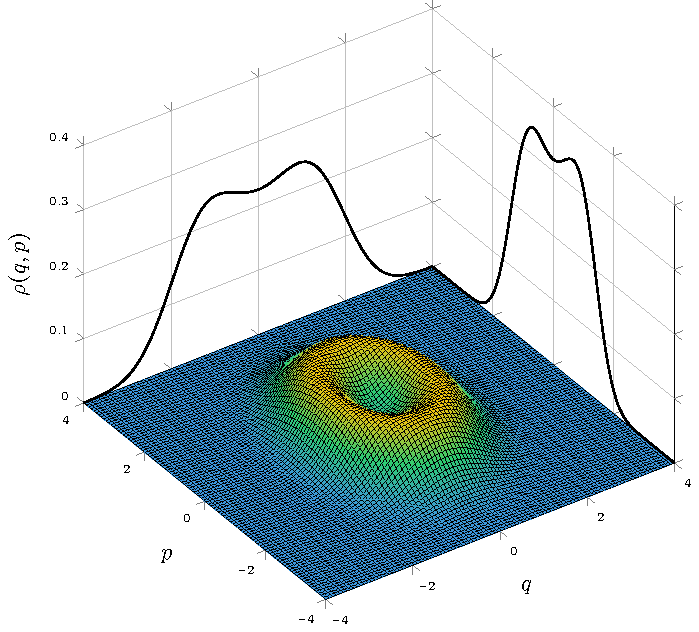
\includegraphics{media/other/time_averaged_ho.pdf}
    \caption{Numerical solution of the time-averaged distribution given by \cref{eq:time_averaged_pq}, for $m = 1$, $k = 2$, $\Sigma = \mqty(0.2 & 0.1 \\ 0.1 & 0.2)$ and $\vec{x}_0 = \mqty(1\\1)$. The marginalized distributions for $p$ and $q$ are shown as well.}
    \label{fig:time_average_ho}
\end{figure}
\Cref{eq:time_averaged_pq} may be solved analytically for a simple case (normalized units and diagonal covariance), where the final solution is expressed in terms of the modified Bessel functions.\footnote{In this case $\Phi$ becomes an orthogonal matrix, which considerably simplifies the evaluation of the integral; the time-dependent argument of the exponential then reverts to a simple rotation, which can then be solved using the integral identity:
    $$ \int^{2\pic}_0 \ec^{A\cos(\varphi) + B\sin(\varphi)}\dd{\varphi} = 2\pic I_0\qty(\sqrt{A^2 + B^2}),  $$
$I_0$ being the modified Bessel function of the first kind \cite{Gradshteyn2007}.
}

\paragraph{Energy distribution} The energy distribution is a generalized chi-squared distribution, because it is a general quadratic form of a normally distributed vector with nonzero mean \cite{Das2021}.

\chapter{Damped harmonic oscillator}
In their most traditional fashion, the Hamiltonian and Lagrangian treatments of mechanical systems do not incorporate energy dissipation; that is, they assume the conservation of (mechanical) energy in the system. The classical theory does allow for an optional explicit time-dependence of the Hamiltonian and Lagrangian, but although this may allow one to incorporate dissipation, it is no direct solution for the dissipation problem. Although this may seem odd from the perspective of the engineering field, where dissipation really is the rule rather than the exception, dissipation is arguably not of primary concern for physicists. This is because dissipation is considered to be a \emph{macro-phenomenon}; that is, it arises because one chooses not to model certain degrees of freedom in the system, while physicists are often concerned with ideal system descriptions on the macro-scale. Nonetheless, the celebrated report by \citet{Dekker1981} provides an overview of the (often fruitful) attempts that have been made to include dissipation in the Hamiltonian and Lagrangian description; the former may allow one to consider dissipation on the quantum level as well --- this is beyond the scope of this text. In addition to these methods, recent developments in the economic engineering group have proposed two new methods to deal with linear damping in mechanical systems, see \citet{Hutters2020a} and \citet{Mendel2021}. In the following section, these methods are placed in a slightly more rigorous (read: geometric) context, after which they serve as the apparatus for the Liouville equation on the damped harmonic oscillator.

\section{A quick tour of dissipative classical mechanics}
\begin{figure}[ht]
    \centering
    \begin{tikzpicture}[every node/.style={outer sep=0pt,thick}]
    \tikzstyle{spring}=[thick,decorate,decoration={zigzag,pre length=0.3cm,post length=0.3cm,segment length=6}]
    \tikzstyle{damper}=[thick,decoration={markings,  
      mark connection node=dmp,
      mark=at position 0.5 with 
      {
        \node (dmp) [thick,inner sep=0pt,transform shape,rotate=-90,minimum width=15pt,minimum height=3pt,draw=none] {};
        \draw [thick] ($(dmp.north east)+(2pt,0)$) -- (dmp.south east) -- (dmp.south west) -- ($(dmp.north west)+(2pt,0)$);
        \draw [thick] ($(dmp.north)+(0,-5pt)$) -- ($(dmp.north)+(0,5pt)$);
      }
    }, decorate]
    \tikzstyle{ground}=[fill,pattern=north east lines,draw=none,minimum width=0.75cm,minimum height=0.3cm]

    \node (M) [draw,minimum width=1cm, minimum height=1.5cm] {$m$};

    \node (ground) [ground,anchor=north,yshift=-0.25cm,minimum width=1.5cm] at (M.south) {};
    \draw (ground.north east) -- (ground.north west);
    \draw [thick] (M.south west) ++ (0.2cm,-0.125cm) circle (0.125cm)  (M.south east) ++ (-0.2cm,-0.125cm) circle (0.125cm);

    \node (wall) [ground, rotate=-90, minimum width=2cm,yshift=-3cm] {};
    \draw (wall.north east) -- (wall.north west);

    \draw [spring] (wall.160) -- ($(M.north west)!(wall.160)!(M.south west)$) node[pos=0.5,anchor=south, outer sep=4pt] {$k$};
    \draw [damper] (wall.20) -- ($(M.north west)!(wall.20)!(M.south west)$) node[pos=0.5,anchor=north, outer sep=10pt] {$b$};

    \path (wall) ++(0.1cm, 1.2cm) -| node (q) {} (M);
    \draw[|->] (wall) ++(0.2cm, 1.2cm) -- (q.center) node[pos=0.5, anchor=south] {$q$};
    \draw (q) ++(0, 0.1cm) -- ++(0, -0.5cm);

    \node[bgelement] (J1) at (4.5, -1) {1};
    \node[bgelement, label=north:$k$] (C) at (4.5, 0.5) {C};
    \node[bgelement, label=east:$m$]  (I) at (6, -1) {I};
    \node[bgelement, label=west:$b$]  (R) at (3, 0.5) {R};

    % test
    \draw[bonds] 
        (J1) edge[e_out] (I)
        (J1) edge[f_out] (R)
        (J1) edge[f_out] (C);


\end{tikzpicture}

    \caption{Schematic of the damped harmonic oscillator.}
    \label{fig:dho}
\end{figure}

The damped harmonic oscillator considered in this text is the one that features a damper `in parallel' with the spring, as shown in \cref{fig:dho}. The corresponding second-order differential equations are:\footnote{Although a linear potential force is assumed here, this treatment generalizes to any potential function $U = U(q, t)$ that does not involve the generalized velocity in a straightforward manner.}
\begin{equation}
    \dv{}{t}\mqty(q\\\dot{q}) = \mqty(0 & 1/m\\-k/m & -b/m)\mqty(q\\\dot{q}) \quad \text{or}\quad m\ddot{q} + b\dot{q} + kq = 0.
    \label{eq:dho}
\end{equation}
The state-transition matrix has eigenvalues
$$ \lambda = \frac{1}{2}\qty(-\frac{b}{m}\pm\sqrt{\qty(\frac{b}{m})^2 - 4\frac{k}{m}}) $$
which is often expressed in `polar coordinates', using the \emph{damping ratio} $\zeta$ and the \emph{undamped natural frequency} $\Omega$:
$$ \lambda = -\Omega \qty(\zeta \pm \ii\sqrt{1 - \zeta^2}) $$
Moreover, the system is assumed to be underdamped, or equivalentl $\zeta < 1$. Solutions are then of the form
$$ $$

\section{Lagrangian mechanics}
\label{sec:mendel_lagrangian}
The method proposed by \citet{Mendel2021} is closely related to the time-dependent Caldirola-Kanai Hamiltonian (as mentioned, the corresponding Lagrangian was already devised by Bateman in 1931 \cite{Bateman1931, Dekker1981}). However, there are some important differences: the time-dependent method takes the dissipation into account simply wrapping the Lagrangian with an exponential discount function so as to include the real part of the eigenvalues into the solution.
\towrite{discuss contribution}

This approach for Lagrangian systems to damped systems (the prototypical example here is, of course, the damped harmonic oscillator) revolves around the definition of a nonstandard Lagrangian function on an extended configuration space. Instead of only position $q$, the extended configuration space is a pair that fixes both position and time. The extended space is denoted by $M$, consequently $m \in M$ has natural coordinates $(q, t)$. Hence, whereas the standard configuration manifold is one-dimensional, it is now two-dimensional, which means the corresponding tangent and cotangent bundles are four-dimensional\footnote{The inclusion of time into the configuration space (or phase space in the Hamiltonian context) is a recurring theme in many important works for various reasons. For example \citet[p. 90]{Arnold1989} uses it to apply the Noether theorem to time-invariance, while \cite[p. 332]{Burke1985} uses it to treat time-dependent systems as if they were time-independent (this is essentially equivalent to the method given here). As is discussed later in this section, \citet{Dirac1950} touches upon it in his discussion of homogeneous Lagrangians and the Legendre transform thereof.}.

Because $t$ defines the configuration of the system, it is not an independent coordinate; that is, it can be varied at will. The independent coordinate is denoted by $\tau$, also referred to as the `path indexation variable', for that is its only significance. \citet{Mendel2021} calls this \emph{proper time} as a testament to its parallel in the theory of special relativity \cite{Landau1971}.

Traditionally, Lagrangian mechanics is staged in the tangent bundle to the configuration manifold. The notation used in this section is something of a delicate matter, sinds the traditional dot notation for tangent vectors usually refers to the actual time $t$, not $\tau$. It is considered undesirable to break with this convention, which is why the tangent velocity vectors with respect to the $q$ and $t$-coordinate are denoted by $v_q$ and $v_t$ respectively. Hence, the tangent bundle at issue has the chart-induced coordinates $(q, t, v_q, v_t)$. As \citet{Burke1985} points out, for (proper) time-dependent systems, it is more natural to look at the contact bundle $\contact{M}$ rather than the tangent bundle $\tangent{M}$ because it makes it possible to deal with the explicit $\tau$-dependence directly. Hence, consider the line-element contact bundle $C\!Q$ with projection map $\pi$,
$$ C\!M \xrightarrow{\pi} M \quad\text{with}\quad \pi: (\tau, q, t, v_q, v_t) \mapsto (\tau, q, t). $$
The idea is, again, now to establish a differential ideal (like in \cref{ssec:ho_liouville_solution}) whose integral manifolds are the solution trajectories of the damped harmonic oscillator system. Although it is not specifically required to use this approach, it helps to sort out some delicacies that appear in taking derivatives that would otherwise be concealed as a consequence of ambiguities in the Leibniz notation.

There are seven forms that constitute the differential ideal:
\begin{itemize}
    \item Two 1-forms, $\alpha_1$ and $\alpha_2$ define the contact structure. Roughly speaking, they provide the `bookkeeping' of the derivatives. The larger spaces $\contact{M}$ and $\tangent{M}$ essentially offer too much `freedom': not every curve in these spaces coincides to lifted version of the solution curve on $M$. Said otherwise, they guarantee tangency (or contact) when the solution trajectory is brought down to the configuration manifold. These 1-forms are:
    \begin{equation} 
        \begin{split}
            \alpha_1 &= \dd{q} - v_q\dd{\tau}\\
            \alpha_2 &= \dd{t} - v_t\dd{\tau}.
        \end{split}
    \end{equation}
    \item Secondly, there are two 1-forms that provide the mechanics of the system. This is where the `proper' Lagrangian comes in to play. The proper Lagrangian $\mathscr{L}$ is defined as a discounted version of the naive Lagrangian $L$ which one would use for an undamped system by taking the difference of the kinetic and potential energy of the system. The naive Lagrangian is equal to $$ L = \frac{1}{2}m\dot{q}^2 - \frac{1}{2}kq^2. $$
    However, as a consequence of the extended phase space $\dot{q}$ does not represent a generalized velocity. By means of the chain rule, it can readily be expressed as a function of $v_q$ and $v_t$:
    $$ \dot{q} = \frac{v_q}{v_t}, $$
    which allows to take derivatives with respect to the chosen coordinates of $\contact{M}$. The proper Lagrangian $\mathscr{L}$ is defined as:
        $$ \mathscr{L}:\,\tangent{M}\to\real : (q, t, v_q, v_t) \mapsto \equiv v_t L(q, t, v_q, v_t), $$
    that is, the Lagrangian is `discounted' by $v_t$. The term discounting is used here because the solution of $v_t$ will turn out to be an exponential, which makes it analogous to the practice of discounting in economics and finance.
\end{itemize}

\section{Legendre transform}
\label{sssec:mendel_legendre}
The usual story in classical mechanics professes that the Lagrangian representation is equivalent to the Hamiltonian representation, which are connected through the so-called Legendre transform. From a geometric perspective, the Legendre transform switches the Lagrangian function on the tangent bundle in favour of the Hamiltonian function on the cotangent bundle, or vice versa. Along with the transformed function, the associated \emph{variational problem} in the Lagrangian setting converts to the integration of the Hamiltonian vector field generated by the Hamiltonian function. In physics, the deeper signifance of the Legendre transform is often discarded in favour of the expression $\dot{q}^ip_i - L$, which only holds when the Lagrangian is strictly convex, or hyperregular, and assuming on-the-fly that $p_i \equiv \partial L/\partial\dot{q}^i$. In this text a more geometric approach is taken in accordance with \citet{Abraham1978}, where the concept of the `fiber derivative' if favoured over the Legendre transform. For well-behaved Lagrangians the traditional notion of the fiber derivative and the Legendre transform coincide; but if not, there are some subtle complications that are relevant for this discussion. 

As mentioned, the Legendre transform (or fiber derivative) `preserves information' --- that is, it is involutive and unique --- if the the function at issue is strictly convex. The Hessian of $\mathscr{L}$ with respect to the generalized velocities is
$$ \mqty(\pdv[2]{L}{\dot{q}}{v_q} & \pdv[2]{L}{\dot{q}}{v_t} \\ \pdv[2]{L}{\dot{q}}{v_t} & \pdv{}{v_t}\qty(L - \pdv{L}{\dot{q}}\dot{q}) ) = \mqty(\pdv[2]{L}{\dot{q}}{v_q} & \pdv[2]{L}{\dot{q}}{v_t} \\ \pdv[2]{L}{\dot{q}}{v_t} & -\pdv[2]{L}{\dot{q}}{v_t}\dot{q}) = \mqty(\pdv{p}{v_q} & \pdv{p}{v_t} \\ \pdv{p}{v_t} & -\pdv{p}{v_t}\dot{q}) $$
such that the determinant of this Hessian is
$$ \pdv{p}{v_q}\dot{q}\,\pdv{p}{v_t} - \qty(\pdv{p}{v_t})^2\; \stackrel{\footnotemark}{=}\; \qty(\pdv{p}{v_t})^2 - \qty(\pdv{p}{v_t})^2 = 0, $$
\footnotetext{Because $\displaystyle \pdv{p}{v_q}\dot{q}=\pdv{p}{v_t}\pdv{v_t}{\dot{q}}\pdv{\dot{q}}{v_q}\dot{q} = \pdv{q}{v_t}\frac{-v_q}{\dot{q}^2}\frac{1}{v_t}\dot{q} = -\pdv{p}{v_t}$.}i.e. the Hessian is singular and has one vanishing eigenvalue; because the other eigenvalue is positive (the trace of the Hessian can be shown to be positive if $v_t$ is), the Hessian is positive semidefinite. This prevents one to easily effect the Legendre transform of $\mathscr{L}$, for this Hessian is the Jacobian of the fiber derivative $\mathbb{F}\mathscr{L}$, which means that the fiber derivative does not provide a bijective mapping beteen the tangent and cotangent bundles (cf. the implicit function theorem). For the damped harmonic oscillator, the fiber derivative results in
\begin{equation}
    \begin{split}
        p \equiv&\,\pdv{\mathscr{L}}{v_q} = m\frac{v_q}{v_t} \\
        W \equiv&\,\pdv{\mathscr{L}}{v_t} = -\frac{1}{2}\qty(m\qty(\frac{v_q}{v_t})^2 + kq^2).
    \end{split}
    \label{eq:fiber_derivative_dho}
\end{equation}

\Cref{eq:fiber_derivative_dho} shows that there is no unique way to assign the velocity pair $(v_q,\,v_t)$ to a conjugate momentum pair $(p, W)$ through the fiber derivative. Indeed, as discussed by \citet[p. 122]{Cannas2001}, \emph{strict convexity} of a function $\mathscr{L}$, that is, the Hessian of $\mathscr{L}$ be positive definite, is required for the Legendre transform to be a diffeomorphism between $TQ$ and $\cotangent{Q}$. The root of this issue can be found in the fact that $p$, $W$ only depend on $\dot{q}$, which fixes only the relative proportion between $v_q$ and $v_t$ --- roughly speaking, it acts on the \emph{projectivization} of the cotangent space, as shown in \cref{fig:fiber_derivative}.
\begin{figure}[h]
    \centering
    \begin{tikzpicture}
    \draw[->] (-1.5, 0) -- (1.5, 0) node[anchor=west] {$v_q$};
    \draw[->] (0, -1.5) -- (0, 1.5) node[anchor=south] {$v_t$};
    \node at (1, -1) {$T_x Q$};
    
    \draw[thick] (0.86603, 0.5) -- (-0.86603, -0.5);
    \draw[thick] (0.70711, 0.70711) -- (-0.70711, -0.70711);
    \draw[thick] (0.5, 0.86603) -- (-0.5, -0.86603);
    \draw[<-] ( $({0.86603*1.2}, {0.5*1.2})$ ) arc (30:60:1.2) node[pos=0.5, anchor=south west] {$\dot{q}$};
    
    \draw[thick] (5, 0) circle (1) node {$\mathbb{RP}^1$};
    \node at (3, 0) {\large{$\cong_\text{hom}$}};
    
    \draw[->] (7.5, 0) -- (10.5, 0) node[anchor=west] {$p$};
    \draw[->] (9, -1.5) -- (9, 1.5) node[anchor=south] {$W$};
    \draw[thick, domain=-1:1] 
        plot ({9 + \x}, {-\x*\x - 0.5} ) node[anchor=south west] {$\text{im}_{\mathbb{F}\mathscr{L}}\,\{T_x Q\}$};
    \node at (10, 1) {$T_x^*\!Q$};
    \draw[->] (1.5, 1) .. controls (3, 1.5) and (6 , 1.5) .. (8, 1) node[pos=0.5, anchor=south] {$\mathbb{F}\mathscr{L}$};
\end{tikzpicture}

    \label{fig:fiber_derivative}
    \caption{Graphical illustration of the singularity of the Lagrangian. The fiber derivative provides a pointwise mapping between the cotangent space $T_xQ$, where $x = (q,\,t)$, and the cotangent bundle $T^*_x\!Q$, but this mapping is neither injective nor surjective. The mapping $\mathbb{F}\mathscr{L}$ acts injectively on the projectivization of the tangent space --- in this case, $\real^2 / \sim$, where $\sim$ denotes the equivalence relation $(v_q, v_t) \sim (\lambda v_q, \lambda v_t) $ ---  it takes the equivalence classes $[v_q : v_t]$ as an argument. Furthermore, the image of the entire tangent space is restricted to a parabolic subset of the cotangent space.}
\end{figure}

All of this boils down to the fact that the fiber derivative/Legendre transform is unable to express the transformed Lagrangian function completely in terms of the coordinates of the cotangent bundle. In this case, the Lagrangian function is called \emph{degenerate} or \emph{singular}; Lagrangians for which the fiber derivative produces a global diffeomorphism are called \emph{hyperregular} \cite[p. 236]{Abraham1978}.

An additional observation is that the Lagrangian $\mathscr{L}$ is \emph{homogeneous of the first degree} in the generalized velocities $v_q$ and $v_t$; i.e. multiplication of all velocities by a factor $\lambda$ is equal to multiplying the Lagrangian itself by that factor (to the `first power', hence the first degree). This is, as discussed by \citet{Abraham1978} and \citet{Dirac1950}, a classical example of a singular Lagrangian. This makes the homogeneous Lagrangian function subject to the Euler theorem (on homogeneous functions); which means that the Lagrangian is a linear combination of its partial derivatives with respect to the generalized velocities \cite{Dirac1950}. Given that the Lagrangian is homogeneous, the Euler theorem asserts that
$$ \mathscr{L} = v_q \pdv{\mathscr{L}}{v_q} + v_t \pdv{\mathscr{L}}{v_t} = v_q p + v_t W. $$
Substitution by the found expressions for $p$ and $W$ indeed recovers the original definition of the discounted Lagrangian. The point is though, that the above is \emph{precisely} equal to the duality pairing that is used for the Legendre transform; as such, a `naive' Legendre transform $v_q p + Wv_t - \mathscr{L}$ will simply vanish in the strong fashion. Hence, according to the Dirac method,
$$ H = v\phi $$
where $\phi$ is the first-order constraint
$$ W + \frac{1}{2m}p^2 + \frac{1}{2}kq^2 = 0 $$

\begin{aside}{Singular Lagrangians and the Dirac method}
    As mentioned, singular Lagrangians are Lagrangians for which the mass matrix
    $$ \qty[\pdv{\mathscr{L}}{\dot{q}_i}{\dot{q_j}}]$$
    is rank-deficient. With slight abuse of notation, $L$ denotes a general Lagrangian and $\dot{q}$ the corresponding generalized velocities. This prevents one from finding the corresponding Hamiltonian representation in the traditional fashion using the Legendre transform, since this entire process hinges on the above Hessian to provide a bijective mapping between the tangent and cotangent spaces (pointwise), that is, to find a mapping between velocities and momenta. Paul Dirac developed a method to overcome this problem, as discussed by \citet{Dirac1950}, \citet{Kunzle1969}, and \citet{Cisneros-Parra2012}. It is interesting to note that the last author considers degeneracy to be a property reserved for `artificial' Lagrangians; by which he means those which do not correspond to real mechanical systems. This claim is, of course, refuted by the Mendel approach given in this text.

    Because of the singularity of the Hessian, there must be a number of conditions on the conjugate momenta such that there remains an additional dependence between the conjugate momenta:
    $$ \phi_k(\vec{p}, \vec{q}, t) = 0. $$
    Using Dirac's method, the resulting Hamiltonian is of the form: \cite{Cisneros-Parra2012}
    $$ H = H_0 + \sum_k v_k \phi_k, $$
    where $H_0$ denotes the `naive' Hamiltonian found by taking a straightforward Legendre transform, and $v_k$ new independent variables (i.e, additional coordinates of the cotangent space as to span its entirety). Aside from the \emph{primary restrictions} $\phi_k$, the Dirac method also imposes a consistency condition of the form 
    $$ \dot{\phi}_k = 0, $$
    from which the \emph{secondary restrictions} are obtained.

    Make sure to read \url{https://en.wikipedia.org/wiki/First_class_constraint#Geometric_theory} for a geometric interpretation.

    NOTE: Max uses `vanish identically', is the same as strong/weak equality by Dirac
\end{aside}

The Lagrangian 1-form is the pullback of the tautological 1-form under the fiber derivative. Lagrangian 1-form and 2-form, economic interpretation: market elasticities. Lagrange 2-form contains the market elasticities, quite literally the geometric encoding of the corresponding bond graph.
    
\subsection{Hamiltonian mechanics}
\label{sssec:mendel_hamiltonian}
In this section, the method proposed by \citet{Mendel2021} is used to deal with the problem of dissipative systems in the framework of Hamiltonian mechanics. The prototypical example that is the harmonic oscillator with a linear (parallel) damping element. As noted, using a time-dependent Hamiltonian to include dissipative mechanics is not quite a new idea (cf. \citet{Dekker1981}), but the salient point here is the \emph{symplectization} of the contact structure that normally underlies such a system. That is to say, there is an additional dimension on top of $p, q, t$ to allow the manifold to be symplectic in the first place. For the damped harmonic oscillator, this boils down to a 2-dimensional configuration manifold $Q$ with coordinates $(q,\,t)$, with at each point attached a cotangent space which contains elements of the form $\alpha\dd{q} + \beta\dd{t}$. To turn the cotangent bundle into a symplectic manifold by virtue of the bundle structure, define the tautological 1-form
$$ \alpha = p\dd{q} + W\dd{t} \quad \alpha \in \cotangent{(\cotangent{Q})},$$
from which the symplectic 2-form is obtained:
$$ \omega = -\dd{\alpha} = \wedgep{\dd{q}}{\dd{p}} + \wedgep{\dd{t}}{\dd{W}}.$$
This results in a four-dimensional symplectic manifold $(M, \omega)$. 

\subsection{Multi-degree of freedom systems}
As noted by \citet{Udwadia2013}, the general solution of the `inverse problem' in Lagrangian mechanics becomes quickly intractable if the number of degrees of freedom in the grows (although the Helmholtz equations theoretically guarantee a solution). For linear systems, this can be easily understood from simple ideas in linear systems theory (which is not mentioned in the work of \citet{Udwadia2013}). The differential equation of the matrix solution for a general mechanical system has the form:
$$ \mqty(\vec{q}\\\vec{\dot{q}}) = \mqty(0 & I \\ -M^{-1}K & -M^{-1}B) $$
where $M$, $K$ and $B$ are the mass matrix, stiffness matrix and damping matrix respectively. Now, finding the `exponential envelope' that is used in the Caldirola-Kanai style Lagrangians or Hamiltonians becomes a complicated matter in the general case: one needs to decouple the system into individual solutions, each with its discount factor. Naturally, this coincides precisely with an eigenvalue decomposition of the system, i.e.
$$ \mqty(\vec{q}\\\vec{p}) = T\exp(J)T^{-1}\mqty(\vec{q}_0\\\vec{p}_0). $$
If one assumes that all the system dynamics are underdamped and the matrix $A$ is simple, then the $J$ is diagonal with complex entries (each of which is paired with its complex conjugate). This is equivalent to a linear combinations of solutions $e^{\gamma t}\qty(c_1\cos(\Omega t) + c_2\sin(\Omega t))$. Theoretically, one can find a Lagrangian for all the decoupled parts, each with their own discount `envelope' to formulate the Lagrangian of the overall problem. Unfortunately, this is not possible in a closed-form fashion (only up to two degrees of freedom in general, for which it is the maximal polynomial order to which a closed form solution exist for the roots). One could however construct a `numerical Lagrangian', by computing the eigenvalues given the parameters. Of course, this does not make the solution of the ODE's easier, but it the Lagrangian itself can help to offer insights in the nature of the system.

\subsection{Complex Hamiltonian}
Coen's method

\part{Non-autonomous Systems}
\chapter{Bla bla}

%========================== Appendices =======================================

\appendix
% An Appendix
\chapter{Symplectic geometry}

\section{Exterior calculus}

An \emph{exterior form of degree} $k$ or $k$-\emph{form} is a $k$-linear antisymmetric function of $k$ vectors
$$ \omega(\alpha \xi_1 + \beta_1\eta_1,\,\xi_2,\, \ldots,\, \xi_k) = \alpha_1\omega\qty(\xi_1,\, \xi_2,\, \ldots,\, \xi_k) 
   + \beta_1\omega(\eta_1,\, \xi_2,\, \ldots,\, \xi_k)$$ 
and 
$$ \omega(\xi_{\pi(1)},\, \ldots,\, \xi_{\pi(k)}) = \sgn(\pi)\omega(\xi_1,\, \ldots,\, \xi_k) $$
i.e. $\omega \in \Lambda^k(V)$. The space of $k$-forms on $V$ is equal to the antisymmetric projection
$$ \Lambda^k(V) = \mathscr{P}_-(V\otimes\ldots\otimes V) $$
where
$$ \mathscr{P}_-(v_1\otimes\ldots\otimes v_k) = \frac{1}{k!}\sum_{\pi\in S_k} v_{\pi(1)}.$$

The \emph{exterior product} $\wedgep{\omega^k}{\omega^\ell}$ of $k$-form $\omega^k$ and $\ell$-form $\omega^\ell$ is a 
$(k + \ell)$-form . The action of $\wedgep{\omega^k}{\omega^\ell}$ on a vector of form $ v_1 \otimes \ldots \otimes v_{k+\ell}$
is given by 
$$ (\wedgep{\omega^k}{\omega^\ell})(v_1 \otimes \ldots \otimes v_{k+\ell}) 
   = \frac{1}{k!}\frac{1}{\ell!} \sum_{\pi \in S_k} \sgn(\pi)\omega^{k}(v_{\pi(1)} \otimes \ldots \otimes v_{\pi(k)})
     \omega^\ell(v_{\pi(k+1)} \otimes \ldots \otimes v_{\pi(k+\ell)}). $$
Furthermore, the exterior product has the following properties:
\begin{itemize}
    \item \emph{skew-commutativity}:  $ \wedgep{\omega^k}{\omega^\ell} = (-1)^{k\ell}\,\wedgep{\omega^\ell}{\omega^k}$
    \item \emph{distributivity}: $ \wedgep{(\alpha \omega_1^k + \beta\omega^k_2)}{\omega^\ell} = 
                                   \alpha\,\wedgep{\omega_1^k}{\omega^\ell} + \beta\, \wedgep{\omega^k_2}{\omega^\ell} $ 
    \item \emph{associativity}: $ \wedgep{\qty(\wedgep{\omega^k}{\omega^\ell})}{\omega^m} = \wedgep{\omega^k}{\qty(\wedgep{\omega^\ell}{\omega^m})}$
\end{itemize}



%========================== Back matter ======================================

\backmatter

%\bibliographystyle{ieeetr}      % This style puts references in order of appearance
%\bibliographystyle{plain}      % This style puts references in alphabetic order
\printbib{library}

%
% Glossary
\chapter{Glossary} %
%
%\printacronyms
%\begin{acronym}[\hspace{0.8in}] % 0.8in is also used by the nomenclature
%	\acro{3mE}[3\textlarger{m}E]{Mechanical, Maritime and Materials Engineering}%
%	\acro{AMS}{American Mathematical Society}%
%	\acro{DCSC}{Delft Center for Systems and Control}%
%	\acro{TU}[TU D\textlarger{elft}]{Delft University of Technology}%
%\end{acronym}%
%
% Nomenclature

  %\ifstrequal{#1}{G}{General}{%
  %\ifstrequal{#1}{E}{Economic Engineering}{%
  %\ifstrequal{#1}{C}{Contact geometry}{}}}%%
  %\ifstrequal{#1}{S}{Split-quaternions}{%%

    % Nomenclature test

%    \nomenclature[G]{$p$}{Momentum}
%    \nomenclature[S]{$\spquaternions$}{Split-quaternions}
%    \nomenclature[C]{$\alpha$}{Contact form}
%
%\printnomenclature

\section*{Economic symbols}
% Greek symbols
\begin{tabular}{p{0.1\textwidth}p{0.5\textwidth}}
% --------- Letter symbols
% ---------- Groups
% ---------- Other symbols
\end{tabular}

\section*{Physical symbols}
% Greek symbols
\begin{itemize}[itemsep=0pt, leftmargin=2cm, labelsep=0cm, labelwidth=1.9cm, align=left]
    \item[$\beta$] Work 1-form
    \item[$\gamma$] Damping coefficient
    \item[$\eta$] Heat 1-form
%
% --------- Letter symbols
    \item[$E$] (Mechanical) energy
    \item[$n_\text{s}$] Amount of substance
    \item[$P$] Pressure
    \item[$p$] Momentum
    \item[$q$] Position
    \item[$R_\text{g}$] Universal gas constant
    \item[$S$] Entropy
    \item[$T$] Temperature
    \item[$U$] Internal energy
    \item[$V$] Volume
%
% ---------- Number sets
%
% ---------- Groups
%
% ---------- Other symbols
\end{itemize}
\section*{Mathematical symbols}
% Greek symbols
\begin{itemize}[itemsep=0pt, leftmargin=2cm, labelsep=0cm, labelwidth=1.9cm, align=left]
    \item[$\alpha$] General contact 1-form
    \item[$\omega$] Symplectic 2-form
    \item[$\theta$] Liouville 1-form
%
% --------- Letter symbols
    \item[$M$] Phase space; general manifold
    \item[$Q$] Configuration space
%
% ---------- Number sets
    \item[$\real^n$] Real coordinate space of dimension $n$
%
% ---------- Groups
%
% ---------- Other symbols
    \item[$\wedgep{}{}$]  Wedge (or exterior) product
    \item[$\intpr{}{}$]  Interior product
    \item[$\dd{}$]  Exterior derivative
    \item[$\lied{X}{}$]  Lie derivative with respect to the vector field $X$
    \item[$\otimes$]  Tensor product
    \item[$\bundle{E}{\pi}{B}$]  Bundle with total space $E$, projection map $\pi$ and base space $B$
    \item[$\tspace{x}{M}$]  Tangent space to the manifold $M$ at the point $x$
    \item[$\ctspace{x}{M}$]  Cotangent space of the manifold $M$ at the point $x$
    \item[$\tbundle{M}$]  Tangent bundle of the manifold $M$
    \item[$\ctbundle{M}$]  Cotangent bundle of the manifold $M$
    \item[$\vfields{M}$]  Set of vector fields (smooth sections of \tbundle{M}) on the manifold $M$
    \item[$\functions{M}$]  Set of smooth functions on the manifold $M$
    \item[$\nforms{n}{M}$]  Set of differential $n$-forms on the manifold $M$
\end{itemize}


\cleardoublepage
\printindex

\end{document}
